\documentclass[twoside]{book}

% Packages required by doxygen
\usepackage{fixltx2e}
\usepackage{calc}
\usepackage{doxygen}
\usepackage{graphicx}
\usepackage[utf8]{inputenc}
\usepackage{makeidx}
\usepackage{multicol}
\usepackage{multirow}
\PassOptionsToPackage{warn}{textcomp}
\usepackage{textcomp}
\usepackage[nointegrals]{wasysym}
\usepackage[table]{xcolor}

% Font selection
\usepackage[T1]{fontenc}
\usepackage{mathptmx}
\usepackage[scaled=.90]{helvet}
\usepackage{courier}
\usepackage{amssymb}
\usepackage{sectsty}
\renewcommand{\familydefault}{\sfdefault}
\allsectionsfont{%
  \fontseries{bc}\selectfont%
  \color{darkgray}%
}
\renewcommand{\DoxyLabelFont}{%
  \fontseries{bc}\selectfont%
  \color{darkgray}%
}
\newcommand{\+}{\discretionary{\mbox{\scriptsize$\hookleftarrow$}}{}{}}

% Page & text layout
\usepackage{geometry}
\geometry{%
  a4paper,%
  top=2.5cm,%
  bottom=2.5cm,%
  left=2.5cm,%
  right=2.5cm%
}
\tolerance=750
\hfuzz=15pt
\hbadness=750
\setlength{\emergencystretch}{15pt}
\setlength{\parindent}{0cm}
\setlength{\parskip}{0.2cm}
\makeatletter
\renewcommand{\paragraph}{%
  \@startsection{paragraph}{4}{0ex}{-1.0ex}{1.0ex}{%
    \normalfont\normalsize\bfseries\SS@parafont%
  }%
}
\renewcommand{\subparagraph}{%
  \@startsection{subparagraph}{5}{0ex}{-1.0ex}{1.0ex}{%
    \normalfont\normalsize\bfseries\SS@subparafont%
  }%
}
\makeatother

% Headers & footers
\usepackage{fancyhdr}
\pagestyle{fancyplain}
\fancyhead[LE]{\fancyplain{}{\bfseries\thepage}}
\fancyhead[CE]{\fancyplain{}{}}
\fancyhead[RE]{\fancyplain{}{\bfseries\leftmark}}
\fancyhead[LO]{\fancyplain{}{\bfseries\rightmark}}
\fancyhead[CO]{\fancyplain{}{}}
\fancyhead[RO]{\fancyplain{}{\bfseries\thepage}}
\fancyfoot[LE]{\fancyplain{}{}}
\fancyfoot[CE]{\fancyplain{}{}}
\fancyfoot[RE]{\fancyplain{}{\bfseries\scriptsize Generated on Tue Jan 24 2017 08\+:59\+:06 for Analytics Template Library by Doxygen }}
\fancyfoot[LO]{\fancyplain{}{\bfseries\scriptsize Generated on Tue Jan 24 2017 08\+:59\+:06 for Analytics Template Library by Doxygen }}
\fancyfoot[CO]{\fancyplain{}{}}
\fancyfoot[RO]{\fancyplain{}{}}
\renewcommand{\footrulewidth}{0.4pt}
\renewcommand{\chaptermark}[1]{%
  \markboth{#1}{}%
}
\renewcommand{\sectionmark}[1]{%
  \markright{\thesection\ #1}%
}

% Indices & bibliography
\usepackage{natbib}
\usepackage[titles]{tocloft}
\setcounter{tocdepth}{3}
\setcounter{secnumdepth}{5}
\makeindex

% Hyperlinks (required, but should be loaded last)
\usepackage{ifpdf}
\ifpdf
  \usepackage[pdftex,pagebackref=true]{hyperref}
\else
  \usepackage[ps2pdf,pagebackref=true]{hyperref}
\fi
\hypersetup{%
  colorlinks=true,%
  linkcolor=blue,%
  citecolor=blue,%
  unicode%
}

% Custom commands
\newcommand{\clearemptydoublepage}{%
  \newpage{\pagestyle{empty}\cleardoublepage}%
}


%===== C O N T E N T S =====

\begin{document}

% Titlepage & ToC
\hypersetup{pageanchor=false,
             bookmarks=true,
             bookmarksnumbered=true,
             pdfencoding=unicode
            }
\pagenumbering{roman}
\begin{titlepage}
\vspace*{7cm}
\begin{center}%
{\Large Analytics Template Library }\\
\vspace*{1cm}
{\large Generated by Doxygen 1.8.8}\\
\vspace*{0.5cm}
{\small Tue Jan 24 2017 08:59:06}\\
\end{center}
\end{titlepage}
\clearemptydoublepage
\tableofcontents
\clearemptydoublepage
\pagenumbering{arabic}
\hypersetup{pageanchor=true}

%--- Begin generated contents ---
\chapter{A\+T\+L2}
\label{md__a_t_l2__r_e_a_d_m_e}
\hypertarget{md__a_t_l2__r_e_a_d_m_e}{}
A\+T\+L with redesigned container module 
\chapter{Namespace Index}
\section{Namespace List}
Here is a list of all documented namespaces with brief descriptions\+:\begin{DoxyCompactList}
\item\contentsline{section}{\hyperlink{namespaceatl}{atl} }{\pageref{namespaceatl}}{}
\item\contentsline{section}{\hyperlink{namespaceport}{port} }{\pageref{namespaceport}}{}
\item\contentsline{section}{\hyperlink{namespacers}{rs} }{\pageref{namespacers}}{}
\item\contentsline{section}{\hyperlink{namespacesimd}{simd} }{\pageref{namespacesimd}}{}
\end{DoxyCompactList}

\chapter{Hierarchical Index}
\section{Class Hierarchy}
This inheritance list is sorted roughly, but not completely, alphabetically\+:\begin{DoxyCompactList}
\item \contentsline{section}{anchor}{\pageref{unionanchor}}{}
\item \contentsline{section}{arena$<$ N $>$}{\pageref{classarena}}{}
\item \contentsline{section}{atl\+:\+:Big\+Float$<$ T $>$}{\pageref{classatl_1_1_big_float}}{}
\item \contentsline{section}{port\+:\+:cilist}{\pageref{structport_1_1cilist}}{}
\item \contentsline{section}{atl\+:\+:clfallocator$<$ T $>$}{\pageref{structatl_1_1clfallocator}}{}
\item \contentsline{section}{util\+:\+:Combinations\+With\+Repetition}{\pageref{classutil_1_1_combinations_with_repetition}}{}
\item \contentsline{section}{util\+:\+:Combonations}{\pageref{classutil_1_1_combonations}}{}
\item \contentsline{section}{util\+:\+:compressed\+\_\+vector$<$ T $>$}{\pageref{classutil_1_1compressed__vector}}{}
\item \contentsline{section}{emlib\+:\+:Hash\+Set$<$ Key\+T, Hash\+T, Comp\+T $>$\+:\+:const\+\_\+iterator}{\pageref{classemlib_1_1_hash_set_1_1const__iterator}}{}
\item \contentsline{section}{emlib\+:\+:Hash\+Map$<$ Key\+T, Value\+T, Hash\+T, Comp\+T $>$\+:\+:const\+\_\+iterator}{\pageref{classemlib_1_1_hash_map_1_1const__iterator}}{}
\item \contentsline{section}{atl\+:\+:Container\+Trait$<$ T $>$}{\pageref{structatl_1_1_container_trait}}{}
\item \contentsline{section}{controlblock\+\_\+t}{\pageref{structcontrolblock__t}}{}
\item \contentsline{section}{tools\+:\+:C\+P\+U\+D\+M}{\pageref{classtools_1_1_c_p_u_d_m}}{}
\item \contentsline{section}{desc}{\pageref{structdesc}}{}
\item \contentsline{section}{Divide\+Thread\+Function}{\pageref{struct_divide_thread_function}}{}
\item \contentsline{section}{tools\+:\+:Exception\+D\+M}{\pageref{classtools_1_1_exception_d_m}}{}
\item \contentsline{section}{atl\+:\+:Expression\+Base$<$ R\+E\+A\+L\+\_\+\+T, A $>$}{\pageref{structatl_1_1_expression_base}}{}
\item \contentsline{section}{atl\+:\+:Expression\+Base$<$ double, Variable$<$ double $>$ $>$}{\pageref{structatl_1_1_expression_base}}{}
\begin{DoxyCompactList}
\item \contentsline{section}{atl\+:\+:Variable$<$ double $>$}{\pageref{structatl_1_1_variable}}{}
\item \contentsline{section}{atl\+:\+:Variable$<$ double $>$}{\pageref{structatl_1_1_variable}}{}
\end{DoxyCompactList}
\item \contentsline{section}{atl\+:\+:Expression\+Base$<$ R\+E\+A\+L\+\_\+\+T, A\+Cos$<$ R\+E\+A\+L\+\_\+\+T, E\+X\+P\+R $>$ $>$}{\pageref{structatl_1_1_expression_base}}{}
\begin{DoxyCompactList}
\item \contentsline{section}{atl\+:\+:A\+Cos$<$ R\+E\+A\+L\+\_\+\+T, E\+X\+P\+R $>$}{\pageref{structatl_1_1_a_cos}}{}
\item \contentsline{section}{atl\+:\+:A\+Cos$<$ R\+E\+A\+L\+\_\+\+T, E\+X\+P\+R $>$}{\pageref{structatl_1_1_a_cos}}{}
\end{DoxyCompactList}
\item \contentsline{section}{atl\+:\+:Expression\+Base$<$ R\+E\+A\+L\+\_\+\+T, Add$<$ R\+E\+A\+L\+\_\+\+T, L\+H\+S, R\+H\+S $>$ $>$}{\pageref{structatl_1_1_expression_base}}{}
\begin{DoxyCompactList}
\item \contentsline{section}{atl\+:\+:Add$<$ R\+E\+A\+L\+\_\+\+T, L\+H\+S, R\+H\+S $>$}{\pageref{structatl_1_1_add}}{}
\item \contentsline{section}{atl\+:\+:Add$<$ R\+E\+A\+L\+\_\+\+T, L\+H\+S, R\+H\+S $>$}{\pageref{structatl_1_1_add}}{}
\end{DoxyCompactList}
\item \contentsline{section}{atl\+:\+:Expression\+Base$<$ R\+E\+A\+L\+\_\+\+T, A\+Sin$<$ R\+E\+A\+L\+\_\+\+T, E\+X\+P\+R $>$ $>$}{\pageref{structatl_1_1_expression_base}}{}
\begin{DoxyCompactList}
\item \contentsline{section}{atl\+:\+:A\+Sin$<$ R\+E\+A\+L\+\_\+\+T, E\+X\+P\+R $>$}{\pageref{structatl_1_1_a_sin}}{}
\item \contentsline{section}{atl\+:\+:A\+Sin$<$ R\+E\+A\+L\+\_\+\+T, E\+X\+P\+R $>$}{\pageref{structatl_1_1_a_sin}}{}
\end{DoxyCompactList}
\item \contentsline{section}{atl\+:\+:Expression\+Base$<$ R\+E\+A\+L\+\_\+\+T, A\+Tan$<$ R\+E\+A\+L\+\_\+\+T, E\+X\+P\+R $>$ $>$}{\pageref{structatl_1_1_expression_base}}{}
\begin{DoxyCompactList}
\item \contentsline{section}{atl\+:\+:A\+Tan$<$ R\+E\+A\+L\+\_\+\+T, E\+X\+P\+R $>$}{\pageref{structatl_1_1_a_tan}}{}
\item \contentsline{section}{atl\+:\+:A\+Tan$<$ R\+E\+A\+L\+\_\+\+T, E\+X\+P\+R $>$}{\pageref{structatl_1_1_a_tan}}{}
\end{DoxyCompactList}
\item \contentsline{section}{atl\+:\+:Expression\+Base$<$ R\+E\+A\+L\+\_\+\+T, Ceil$<$ R\+E\+A\+L\+\_\+\+T, E\+X\+P\+R $>$ $>$}{\pageref{structatl_1_1_expression_base}}{}
\begin{DoxyCompactList}
\item \contentsline{section}{atl\+:\+:Ceil$<$ R\+E\+A\+L\+\_\+\+T, E\+X\+P\+R $>$}{\pageref{structatl_1_1_ceil}}{}
\item \contentsline{section}{atl\+:\+:Ceil$<$ R\+E\+A\+L\+\_\+\+T, E\+X\+P\+R $>$}{\pageref{structatl_1_1_ceil}}{}
\end{DoxyCompactList}
\item \contentsline{section}{atl\+:\+:Expression\+Base$<$ R\+E\+A\+L\+\_\+\+T, Cos$<$ R\+E\+A\+L\+\_\+\+T, E\+X\+P\+R $>$ $>$}{\pageref{structatl_1_1_expression_base}}{}
\begin{DoxyCompactList}
\item \contentsline{section}{atl\+:\+:Cos$<$ R\+E\+A\+L\+\_\+\+T, E\+X\+P\+R $>$}{\pageref{structatl_1_1_cos}}{}
\item \contentsline{section}{atl\+:\+:Cos$<$ R\+E\+A\+L\+\_\+\+T, E\+X\+P\+R $>$}{\pageref{structatl_1_1_cos}}{}
\end{DoxyCompactList}
\item \contentsline{section}{atl\+:\+:Expression\+Base$<$ R\+E\+A\+L\+\_\+\+T, Cosh$<$ R\+E\+A\+L\+\_\+\+T, E\+X\+P\+R $>$ $>$}{\pageref{structatl_1_1_expression_base}}{}
\begin{DoxyCompactList}
\item \contentsline{section}{atl\+:\+:Cosh$<$ R\+E\+A\+L\+\_\+\+T, E\+X\+P\+R $>$}{\pageref{structatl_1_1_cosh}}{}
\item \contentsline{section}{atl\+:\+:Cosh$<$ R\+E\+A\+L\+\_\+\+T, E\+X\+P\+R $>$}{\pageref{structatl_1_1_cosh}}{}
\end{DoxyCompactList}
\item \contentsline{section}{atl\+:\+:Expression\+Base$<$ R\+E\+A\+L\+\_\+\+T, Divide$<$ R\+E\+A\+L\+\_\+\+T, L\+H\+S, R\+H\+S $>$ $>$}{\pageref{structatl_1_1_expression_base}}{}
\begin{DoxyCompactList}
\item \contentsline{section}{atl\+:\+:Divide$<$ R\+E\+A\+L\+\_\+\+T, L\+H\+S, R\+H\+S $>$}{\pageref{structatl_1_1_divide}}{}
\item \contentsline{section}{atl\+:\+:Divide$<$ R\+E\+A\+L\+\_\+\+T, L\+H\+S, R\+H\+S $>$}{\pageref{structatl_1_1_divide}}{}
\end{DoxyCompactList}
\item \contentsline{section}{atl\+:\+:Expression\+Base$<$ R\+E\+A\+L\+\_\+\+T, Exp$<$ R\+E\+A\+L\+\_\+\+T, E\+X\+P\+R $>$ $>$}{\pageref{structatl_1_1_expression_base}}{}
\begin{DoxyCompactList}
\item \contentsline{section}{atl\+:\+:Exp$<$ R\+E\+A\+L\+\_\+\+T, E\+X\+P\+R $>$}{\pageref{structatl_1_1_exp}}{}
\item \contentsline{section}{atl\+:\+:Exp$<$ R\+E\+A\+L\+\_\+\+T, E\+X\+P\+R $>$}{\pageref{structatl_1_1_exp}}{}
\end{DoxyCompactList}
\item \contentsline{section}{atl\+:\+:Expression\+Base$<$ R\+E\+A\+L\+\_\+\+T, Fabs$<$ R\+E\+A\+L\+\_\+\+T, E\+X\+P\+R $>$ $>$}{\pageref{structatl_1_1_expression_base}}{}
\begin{DoxyCompactList}
\item \contentsline{section}{atl\+:\+:Fabs$<$ R\+E\+A\+L\+\_\+\+T, E\+X\+P\+R $>$}{\pageref{structatl_1_1_fabs}}{}
\item \contentsline{section}{atl\+:\+:Fabs$<$ R\+E\+A\+L\+\_\+\+T, E\+X\+P\+R $>$}{\pageref{structatl_1_1_fabs}}{}
\end{DoxyCompactList}
\item \contentsline{section}{atl\+:\+:Expression\+Base$<$ R\+E\+A\+L\+\_\+\+T, Floor$<$ R\+E\+A\+L\+\_\+\+T, E\+X\+P\+R $>$ $>$}{\pageref{structatl_1_1_expression_base}}{}
\begin{DoxyCompactList}
\item \contentsline{section}{atl\+:\+:Floor$<$ R\+E\+A\+L\+\_\+\+T, E\+X\+P\+R $>$}{\pageref{structatl_1_1_floor}}{}
\item \contentsline{section}{atl\+:\+:Floor$<$ R\+E\+A\+L\+\_\+\+T, E\+X\+P\+R $>$}{\pageref{structatl_1_1_floor}}{}
\end{DoxyCompactList}
\item \contentsline{section}{atl\+:\+:Expression\+Base$<$ R\+E\+A\+L\+\_\+\+T, Log10$<$ R\+E\+A\+L\+\_\+\+T, E\+X\+P\+R $>$ $>$}{\pageref{structatl_1_1_expression_base}}{}
\begin{DoxyCompactList}
\item \contentsline{section}{atl\+:\+:Log10$<$ R\+E\+A\+L\+\_\+\+T, E\+X\+P\+R $>$}{\pageref{structatl_1_1_log10}}{}
\item \contentsline{section}{atl\+:\+:Log10$<$ R\+E\+A\+L\+\_\+\+T, E\+X\+P\+R $>$}{\pageref{structatl_1_1_log10}}{}
\end{DoxyCompactList}
\item \contentsline{section}{atl\+:\+:Expression\+Base$<$ R\+E\+A\+L\+\_\+\+T, Log$<$ R\+E\+A\+L\+\_\+\+T, E\+X\+P\+R $>$ $>$}{\pageref{structatl_1_1_expression_base}}{}
\begin{DoxyCompactList}
\item \contentsline{section}{atl\+:\+:Log$<$ R\+E\+A\+L\+\_\+\+T, E\+X\+P\+R $>$}{\pageref{structatl_1_1_log}}{}
\item \contentsline{section}{atl\+:\+:Log$<$ R\+E\+A\+L\+\_\+\+T, E\+X\+P\+R $>$}{\pageref{structatl_1_1_log}}{}
\end{DoxyCompactList}
\item \contentsline{section}{atl\+:\+:Expression\+Base$<$ R\+E\+A\+L\+\_\+\+T, Min$<$ R\+E\+A\+L\+\_\+\+T, L\+H\+S, R\+H\+S $>$ $>$}{\pageref{structatl_1_1_expression_base}}{}
\begin{DoxyCompactList}
\item \contentsline{section}{atl\+:\+:Min$<$ R\+E\+A\+L\+\_\+\+T, L\+H\+S, R\+H\+S $>$}{\pageref{structatl_1_1_min}}{}
\end{DoxyCompactList}
\item \contentsline{section}{atl\+:\+:Expression\+Base$<$ R\+E\+A\+L\+\_\+\+T, Multiply$<$ R\+E\+A\+L\+\_\+\+T, L\+H\+S, R\+H\+S $>$ $>$}{\pageref{structatl_1_1_expression_base}}{}
\begin{DoxyCompactList}
\item \contentsline{section}{atl\+:\+:Multiply$<$ R\+E\+A\+L\+\_\+\+T, L\+H\+S, R\+H\+S $>$}{\pageref{structatl_1_1_multiply}}{}
\item \contentsline{section}{atl\+:\+:Multiply$<$ R\+E\+A\+L\+\_\+\+T, L\+H\+S, R\+H\+S $>$}{\pageref{structatl_1_1_multiply}}{}
\end{DoxyCompactList}
\item \contentsline{section}{atl\+:\+:Expression\+Base$<$ R\+E\+A\+L\+\_\+\+T, Pow$<$ R\+E\+A\+L\+\_\+\+T, L\+H\+S, R\+H\+S $>$ $>$}{\pageref{structatl_1_1_expression_base}}{}
\begin{DoxyCompactList}
\item \contentsline{section}{atl\+:\+:Pow$<$ R\+E\+A\+L\+\_\+\+T, L\+H\+S, R\+H\+S $>$}{\pageref{structatl_1_1_pow}}{}
\end{DoxyCompactList}
\item \contentsline{section}{atl\+:\+:Expression\+Base$<$ R\+E\+A\+L\+\_\+\+T, Real$<$ R\+E\+A\+L\+\_\+\+T $>$ $>$}{\pageref{structatl_1_1_expression_base}}{}
\begin{DoxyCompactList}
\item \contentsline{section}{atl\+:\+:Real$<$ R\+E\+A\+L\+\_\+\+T $>$}{\pageref{structatl_1_1_real}}{}
\item \contentsline{section}{atl\+:\+:Real$<$ R\+E\+A\+L\+\_\+\+T $>$}{\pageref{structatl_1_1_real}}{}
\end{DoxyCompactList}
\item \contentsline{section}{atl\+:\+:Expression\+Base$<$ R\+E\+A\+L\+\_\+\+T, Sin$<$ R\+E\+A\+L\+\_\+\+T, E\+X\+P\+R $>$ $>$}{\pageref{structatl_1_1_expression_base}}{}
\begin{DoxyCompactList}
\item \contentsline{section}{atl\+:\+:Sin$<$ R\+E\+A\+L\+\_\+\+T, E\+X\+P\+R $>$}{\pageref{structatl_1_1_sin}}{}
\item \contentsline{section}{atl\+:\+:Sin$<$ R\+E\+A\+L\+\_\+\+T, E\+X\+P\+R $>$}{\pageref{structatl_1_1_sin}}{}
\end{DoxyCompactList}
\item \contentsline{section}{atl\+:\+:Expression\+Base$<$ R\+E\+A\+L\+\_\+\+T, Sinh$<$ R\+E\+A\+L\+\_\+\+T, E\+X\+P\+R $>$ $>$}{\pageref{structatl_1_1_expression_base}}{}
\begin{DoxyCompactList}
\item \contentsline{section}{atl\+:\+:Sinh$<$ R\+E\+A\+L\+\_\+\+T, E\+X\+P\+R $>$}{\pageref{structatl_1_1_sinh}}{}
\item \contentsline{section}{atl\+:\+:Sinh$<$ R\+E\+A\+L\+\_\+\+T, E\+X\+P\+R $>$}{\pageref{structatl_1_1_sinh}}{}
\end{DoxyCompactList}
\item \contentsline{section}{atl\+:\+:Expression\+Base$<$ R\+E\+A\+L\+\_\+\+T, Sqrt$<$ R\+E\+A\+L\+\_\+\+T, E\+X\+P\+R $>$ $>$}{\pageref{structatl_1_1_expression_base}}{}
\begin{DoxyCompactList}
\item \contentsline{section}{atl\+:\+:Sqrt$<$ R\+E\+A\+L\+\_\+\+T, E\+X\+P\+R $>$}{\pageref{structatl_1_1_sqrt}}{}
\item \contentsline{section}{atl\+:\+:Sqrt$<$ R\+E\+A\+L\+\_\+\+T, E\+X\+P\+R $>$}{\pageref{structatl_1_1_sqrt}}{}
\end{DoxyCompactList}
\item \contentsline{section}{atl\+:\+:Expression\+Base$<$ R\+E\+A\+L\+\_\+\+T, Subtract$<$ R\+E\+A\+L\+\_\+\+T, L\+H\+S, R\+H\+S $>$ $>$}{\pageref{structatl_1_1_expression_base}}{}
\begin{DoxyCompactList}
\item \contentsline{section}{atl\+:\+:Subtract$<$ R\+E\+A\+L\+\_\+\+T, L\+H\+S, R\+H\+S $>$}{\pageref{structatl_1_1_subtract}}{}
\item \contentsline{section}{atl\+:\+:Subtract$<$ R\+E\+A\+L\+\_\+\+T, L\+H\+S, R\+H\+S $>$}{\pageref{structatl_1_1_subtract}}{}
\end{DoxyCompactList}
\item \contentsline{section}{atl\+:\+:Expression\+Base$<$ R\+E\+A\+L\+\_\+\+T, Tan$<$ R\+E\+A\+L\+\_\+\+T, E\+X\+P\+R $>$ $>$}{\pageref{structatl_1_1_expression_base}}{}
\begin{DoxyCompactList}
\item \contentsline{section}{atl\+:\+:Tan$<$ R\+E\+A\+L\+\_\+\+T, E\+X\+P\+R $>$}{\pageref{structatl_1_1_tan}}{}
\item \contentsline{section}{atl\+:\+:Tan$<$ R\+E\+A\+L\+\_\+\+T, E\+X\+P\+R $>$}{\pageref{structatl_1_1_tan}}{}
\end{DoxyCompactList}
\item \contentsline{section}{atl\+:\+:Expression\+Base$<$ R\+E\+A\+L\+\_\+\+T, Tanh$<$ R\+E\+A\+L\+\_\+\+T, E\+X\+P\+R $>$ $>$}{\pageref{structatl_1_1_expression_base}}{}
\begin{DoxyCompactList}
\item \contentsline{section}{atl\+:\+:Tanh$<$ R\+E\+A\+L\+\_\+\+T, E\+X\+P\+R $>$}{\pageref{structatl_1_1_tanh}}{}
\item \contentsline{section}{atl\+:\+:Tanh$<$ R\+E\+A\+L\+\_\+\+T, E\+X\+P\+R $>$}{\pageref{structatl_1_1_tanh}}{}
\end{DoxyCompactList}
\item \contentsline{section}{atl\+:\+:Expression\+Base$<$ R\+E\+A\+L\+\_\+\+T, Variable$<$ R\+E\+A\+L\+\_\+\+T $>$ $>$}{\pageref{structatl_1_1_expression_base}}{}
\begin{DoxyCompactList}
\item \contentsline{section}{atl\+:\+:Variable$<$ R\+E\+A\+L\+\_\+\+T $>$}{\pageref{structatl_1_1_variable}}{}
\item \contentsline{section}{atl\+:\+:Variable$<$ R\+E\+A\+L\+\_\+\+T $>$}{\pageref{structatl_1_1_variable}}{}
\end{DoxyCompactList}
\item \contentsline{section}{atl\+:\+:Expression\+Base$<$ T, A $>$}{\pageref{structatl_1_1_expression_base}}{}
\item \contentsline{section}{atl\+:\+:Expression\+Base$<$ T, Fast\+Variable\+Matrix$<$ T, R\+O\+W\+S, C\+O\+L\+U\+M\+N\+S $>$ $>$}{\pageref{structatl_1_1_expression_base}}{}
\begin{DoxyCompactList}
\item \contentsline{section}{atl\+:\+:Fast\+Variable\+Matrix$<$ T, R\+O\+W\+S, C\+O\+L\+U\+M\+N\+S $>$}{\pageref{structatl_1_1_fast_variable_matrix}}{}
\item \contentsline{section}{atl\+:\+:Fast\+Variable\+Matrix$<$ T, R\+O\+W\+S, C\+O\+L\+U\+M\+N\+S $>$}{\pageref{structatl_1_1_fast_variable_matrix}}{}
\end{DoxyCompactList}
\item \contentsline{section}{atl\+:\+:Expression\+Base$<$ T, Variable$<$ T $>$ $>$}{\pageref{structatl_1_1_expression_base}}{}
\begin{DoxyCompactList}
\item \contentsline{section}{atl\+:\+:Variable$<$ T $>$}{\pageref{structatl_1_1_variable}}{}
\item \contentsline{section}{atl\+:\+:Variable$<$ T $>$}{\pageref{structatl_1_1_variable}}{}
\end{DoxyCompactList}
\item \contentsline{section}{atl\+:\+:Expression\+Base$<$ T, Variable\+Matrix$<$ T $>$ $>$}{\pageref{structatl_1_1_expression_base}}{}
\begin{DoxyCompactList}
\item \contentsline{section}{atl\+:\+:Variable\+Matrix$<$ T $>$}{\pageref{structatl_1_1_variable_matrix}}{}
\begin{DoxyCompactList}
\item \contentsline{section}{atl\+:\+:Variable\+Vector$<$ T $>$}{\pageref{structatl_1_1_variable_vector}}{}
\item \contentsline{section}{atl\+:\+:Variable\+Vector$<$ T $>$}{\pageref{structatl_1_1_variable_vector}}{}
\end{DoxyCompactList}
\item \contentsline{section}{atl\+:\+:Variable\+Matrix$<$ T $>$}{\pageref{structatl_1_1_variable_matrix}}{}
\end{DoxyCompactList}
\item \contentsline{section}{atl\+:\+:Expression\+Trait$<$ T $>$}{\pageref{structatl_1_1_expression_trait}}{}
\item false\+\_\+type\begin{DoxyCompactList}
\item \contentsline{section}{rs\+:\+:Lazy\+Flat\+Set$<$ Value, Less, Equal, Sort, Alloc, Is\+Pointer $>$\+:\+:is\+\_\+shared\+\_\+ptr$<$ T $>$}{\pageref{structrs_1_1_lazy_flat_set_1_1is__shared__ptr}}{}
\end{DoxyCompactList}
\item \contentsline{section}{flat\+\_\+map$<$ Key, T $>$}{\pageref{classflat__map}}{}
\item \contentsline{section}{flat\+\_\+set$<$ T, Compare, Allocator $>$}{\pageref{classflat__set}}{}
\item \contentsline{section}{atl\+:\+:Forward\+Mode\+Derivative\+Info$<$ R\+E\+A\+L\+\_\+\+T $>$}{\pageref{structatl_1_1_forward_mode_derivative_info}}{}
\item \contentsline{section}{std\+:\+:hash$<$ emlib\+:\+:Hash\+Cache$<$ T $>$ $>$}{\pageref{structstd_1_1hash_3_01emlib_1_1_hash_cache_3_01_t_01_4_01_4}}{}
\item \contentsline{section}{emlib\+:\+:Hash\+Cache$<$ T $>$}{\pageref{classemlib_1_1_hash_cache}}{}
\item \contentsline{section}{emlib\+:\+:Hash\+Cache$<$ uint32\+\_\+t $>$}{\pageref{classemlib_1_1_hash_cache}}{}
\item \contentsline{section}{emlib\+:\+:Hash\+Map$<$ Key\+T, Value\+T, Hash\+T, Comp\+T $>$}{\pageref{classemlib_1_1_hash_map}}{}
\item \contentsline{section}{emlib\+:\+:Hash\+Map$<$ uint32\+\_\+t, R\+E\+A\+L\+\_\+\+T, emlib\+:\+:Hash\+Cache$<$ uint32\+\_\+t $>$ $>$}{\pageref{classemlib_1_1_hash_map}}{}
\item \contentsline{section}{emlib\+:\+:Hash\+Map\+Equal\+To$<$ T $>$}{\pageref{structemlib_1_1_hash_map_equal_to}}{}
\item \contentsline{section}{emlib\+:\+:Hash\+Set$<$ Key\+T, Hash\+T, Comp\+T $>$}{\pageref{classemlib_1_1_hash_set}}{}
\item \contentsline{section}{emlib\+:\+:Hash\+Set\+Equal\+To$<$ T $>$}{\pageref{structemlib_1_1_hash_set_equal_to}}{}
\item \contentsline{section}{emlib\+:\+:Hash\+Map$<$ Key\+T, Value\+T, Hash\+T, Comp\+T $>$\+:\+:iterator}{\pageref{classemlib_1_1_hash_map_1_1iterator}}{}
\item \contentsline{section}{emlib\+:\+:Hash\+Set$<$ Key\+T, Hash\+T, Comp\+T $>$\+:\+:iterator}{\pageref{classemlib_1_1_hash_set_1_1iterator}}{}
\item \contentsline{section}{rs\+:\+:Lazy\+Flat\+Set$<$ Value, Less, Equal, Sort, Alloc, Is\+Pointer $>$}{\pageref{classrs_1_1_lazy_flat_set}}{}
\item \contentsline{section}{rs\+:\+:Lazy\+Flat\+Set\+Quick\+Sort$<$ Value, Less $>$}{\pageref{structrs_1_1_lazy_flat_set_quick_sort}}{}
\item \contentsline{section}{levelorder\+\_\+vector$<$ T $>$}{\pageref{classlevelorder__vector}}{}
\item \contentsline{section}{atl\+:\+:Line\+Plot$<$ T $>$}{\pageref{classatl_1_1_line_plot}}{}
\item \contentsline{section}{atl\+:\+:Matrix\+Assign$<$ A, T $>$}{\pageref{structatl_1_1_matrix_assign}}{}
\item \contentsline{section}{tools\+:\+:Memory\+D\+M}{\pageref{classtools_1_1_memory_d_m}}{}
\item \contentsline{section}{util\+:\+:Memory\+Pool$<$ T $>$}{\pageref{classutil_1_1_memory_pool}}{}
\item numeric\+\_\+limits\begin{DoxyCompactList}
\item \contentsline{section}{std\+:\+:numeric\+\_\+limits$<$ atl\+:\+:Big\+Float$<$ T $>$ $>$}{\pageref{classstd_1_1numeric__limits_3_01atl_1_1_big_float_3_01_t_01_4_01_4}}{}
\end{DoxyCompactList}
\item \contentsline{section}{procheap}{\pageref{structprocheap}}{}
\item \contentsline{section}{profile\+\_\+entry\+\_\+\+\_\+\+\_\+}{\pageref{structprofile__entry______}}{}
\item \contentsline{section}{tools\+:\+:Profiled\+Function}{\pageref{classtools_1_1_profiled_function}}{}
\item \contentsline{section}{atl\+:\+:Real\+Matrix$<$ T $>$}{\pageref{structatl_1_1_real_matrix}}{}
\item \contentsline{section}{short\+\_\+alloc$<$ T, N $>$\+:\+:rebind$<$ \+\_\+\+Up $>$}{\pageref{structshort__alloc_1_1rebind}}{}
\item \contentsline{section}{atl\+:\+:clfallocator$<$ T $>$\+:\+:rebind$<$ U $>$}{\pageref{structatl_1_1clfallocator_1_1rebind}}{}
\item \contentsline{section}{short\+\_\+alloc$<$ T, N $>$}{\pageref{classshort__alloc}}{}
\item \contentsline{section}{simd\+:\+:simd\+\_\+traits$<$ T $>$}{\pageref{structsimd_1_1simd__traits}}{}
\item \contentsline{section}{simd\+:\+:simd\+\_\+vector$<$ X $>$}{\pageref{classsimd_1_1simd__vector}}{}
\item \contentsline{section}{simd\+:\+:simd\+\_\+vector$<$ vector2d $>$}{\pageref{classsimd_1_1simd__vector}}{}
\begin{DoxyCompactList}
\item \contentsline{section}{simd\+:\+:vector2d}{\pageref{classsimd_1_1vector2d}}{}
\item \contentsline{section}{simd\+:\+:vector2d}{\pageref{classsimd_1_1vector2d}}{}
\item \contentsline{section}{simd\+:\+:vector2d}{\pageref{classsimd_1_1vector2d}}{}
\end{DoxyCompactList}
\item \contentsline{section}{simd\+:\+:simd\+\_\+vector$<$ vector4f $>$}{\pageref{classsimd_1_1simd__vector}}{}
\begin{DoxyCompactList}
\item \contentsline{section}{simd\+:\+:vector4f}{\pageref{classsimd_1_1vector4f}}{}
\item \contentsline{section}{simd\+:\+:vector4f}{\pageref{classsimd_1_1vector4f}}{}
\item \contentsline{section}{simd\+:\+:vector4f}{\pageref{classsimd_1_1vector4f}}{}
\end{DoxyCompactList}
\item \contentsline{section}{simd\+:\+:simd\+\_\+vector\+\_\+traits$<$ X $>$}{\pageref{structsimd_1_1simd__vector__traits}}{}
\item \contentsline{section}{simd\+:\+:simd\+\_\+vector\+\_\+traits$<$ vector2d $>$}{\pageref{structsimd_1_1simd__vector__traits_3_01vector2d_01_4}}{}
\item \contentsline{section}{simd\+:\+:simd\+\_\+vector\+\_\+traits$<$ vector4f $>$}{\pageref{structsimd_1_1simd__vector__traits_3_01vector4f_01_4}}{}
\item \contentsline{section}{sizeclass}{\pageref{structsizeclass}}{}
\item \contentsline{section}{util\+:\+:small\+\_\+set$<$ T, N, C $>$}{\pageref{classutil_1_1small__set}}{}
\item \contentsline{section}{util\+:\+:small\+\_\+vector$<$ Object, N $>$}{\pageref{classutil_1_1small__vector}}{}
\item \contentsline{section}{util\+:\+:small\+\_\+vector$<$ T, N $>$}{\pageref{classutil_1_1small__vector}}{}
\item \contentsline{section}{atl\+:\+:Spin\+Lock}{\pageref{classatl_1_1_spin_lock}}{}
\item \contentsline{section}{atl\+:\+:Stack\+Entry$<$ R\+E\+A\+L\+\_\+\+T $>$}{\pageref{structatl_1_1_stack_entry}}{}
\item \contentsline{section}{atl\+:\+:Streamed\+Data\+File}{\pageref{classatl_1_1_streamed_data_file}}{}
\item \contentsline{section}{atl\+:\+:Tape$<$ R\+E\+A\+L\+\_\+\+T $>$}{\pageref{classatl_1_1_tape}}{}
\item \contentsline{section}{atl\+:\+:Tape$<$ double $>$}{\pageref{classatl_1_1_tape}}{}
\item \contentsline{section}{atl\+:\+:Tape$<$ T $>$}{\pageref{classatl_1_1_tape}}{}
\item \contentsline{section}{Thread\+Function}{\pageref{struct_thread_function}}{}
\item \contentsline{section}{atl\+:\+:Thread\+Pool}{\pageref{classatl_1_1_thread_pool}}{}
\item \contentsline{section}{tools\+:\+:Timer}{\pageref{classtools_1_1_timer}}{}
\item true\+\_\+type\begin{DoxyCompactList}
\item \contentsline{section}{rs\+:\+:Lazy\+Flat\+Set$<$ Value, Less, Equal, Sort, Alloc, Is\+Pointer $>$\+:\+:is\+\_\+shared\+\_\+ptr$<$ std\+:\+:shared\+\_\+ptr$<$ T $>$ $>$}{\pageref{structrs_1_1_lazy_flat_set_1_1is__shared__ptr_3_01std_1_1shared__ptr_3_01_t_01_4_01_4}}{}
\end{DoxyCompactList}
\item type\begin{DoxyCompactList}
\item \contentsline{section}{rs\+:\+:Lazy\+Flat\+Set$<$ Value, Less, Equal, Sort, Alloc, Is\+Pointer $>$\+:\+:is\+\_\+pointer$<$ T $>$}{\pageref{structrs_1_1_lazy_flat_set_1_1is__pointer}}{}
\end{DoxyCompactList}
\item \contentsline{section}{atl\+:\+:Type\+Trait$<$ T $>$}{\pageref{structatl_1_1_type_trait}}{}
\item \contentsline{section}{atl\+:\+:Type\+Trait$<$ atl\+:\+:Variable$<$ double $>$ $>$}{\pageref{structatl_1_1_type_trait_3_01atl_1_1_variable_3_01double_01_4_01_4}}{}
\item \contentsline{section}{atl\+:\+:Type\+Trait$<$ atl\+:\+:Variable$<$ float $>$ $>$}{\pageref{structatl_1_1_type_trait_3_01atl_1_1_variable_3_01float_01_4_01_4}}{}
\item \contentsline{section}{atl\+:\+:Type\+Trait$<$ atl\+:\+:Variable$<$ long double $>$ $>$}{\pageref{structatl_1_1_type_trait_3_01atl_1_1_variable_3_01long_01double_01_4_01_4}}{}
\item \contentsline{section}{atl\+:\+:Variable\+Id\+Generator}{\pageref{classatl_1_1_variable_id_generator}}{}
\item \contentsline{section}{atl\+:\+:Variable\+Info$<$ R\+E\+A\+L\+\_\+\+T $>$}{\pageref{structatl_1_1_variable_info}}{}
\item \contentsline{section}{atl\+:\+:Variable\+Info$<$ double $>$}{\pageref{structatl_1_1_variable_info}}{}
\item \contentsline{section}{atl\+:\+:Variable\+Info$<$ T $>$}{\pageref{structatl_1_1_variable_info}}{}
\item \contentsline{section}{atl\+:\+:Variable\+Matrix\+Assign$<$ T, A $>$}{\pageref{structatl_1_1_variable_matrix_assign}}{}
\item \contentsline{section}{atl\+:\+:Variable\+Info$<$ R\+E\+A\+L\+\_\+\+T $>$\+:\+:V\+I\+Spin\+Lock}{\pageref{classatl_1_1_variable_info_1_1_v_i_spin_lock}}{}
\item \contentsline{section}{atl\+:\+:Wait\+Variable}{\pageref{classatl_1_1_wait_variable}}{}
\end{DoxyCompactList}

\chapter{Class Index}
\section{Class List}
Here are the classes, structs, unions and interfaces with brief descriptions\+:\begin{DoxyCompactList}
\item\contentsline{section}{\hyperlink{structatl_1_1_a_cos}{atl\+::\+A\+Cos$<$ R\+E\+A\+L\+\_\+\+T, E\+X\+P\+R $>$} }{\pageref{structatl_1_1_a_cos}}{}
\item\contentsline{section}{\hyperlink{structatl_1_1_add}{atl\+::\+Add$<$ R\+E\+A\+L\+\_\+\+T, L\+H\+S, R\+H\+S $>$} }{\pageref{structatl_1_1_add}}{}
\item\contentsline{section}{\hyperlink{unionanchor}{anchor} }{\pageref{unionanchor}}{}
\item\contentsline{section}{\hyperlink{classarena}{arena$<$ N $>$} }{\pageref{classarena}}{}
\item\contentsline{section}{\hyperlink{structatl_1_1_a_sin}{atl\+::\+A\+Sin$<$ R\+E\+A\+L\+\_\+\+T, E\+X\+P\+R $>$} }{\pageref{structatl_1_1_a_sin}}{}
\item\contentsline{section}{\hyperlink{structatl_1_1_a_tan}{atl\+::\+A\+Tan$<$ R\+E\+A\+L\+\_\+\+T, E\+X\+P\+R $>$} }{\pageref{structatl_1_1_a_tan}}{}
\item\contentsline{section}{\hyperlink{classatl_1_1_big_float}{atl\+::\+Big\+Float$<$ T $>$} }{\pageref{classatl_1_1_big_float}}{}
\item\contentsline{section}{\hyperlink{structatl_1_1_ceil}{atl\+::\+Ceil$<$ R\+E\+A\+L\+\_\+\+T, E\+X\+P\+R $>$} }{\pageref{structatl_1_1_ceil}}{}
\item\contentsline{section}{\hyperlink{structport_1_1cilist}{port\+::cilist} }{\pageref{structport_1_1cilist}}{}
\item\contentsline{section}{\hyperlink{structatl_1_1clfallocator}{atl\+::clfallocator$<$ T $>$} }{\pageref{structatl_1_1clfallocator}}{}
\item\contentsline{section}{\hyperlink{classutil_1_1_combinations_with_repetition}{util\+::\+Combinations\+With\+Repetition} }{\pageref{classutil_1_1_combinations_with_repetition}}{}
\item\contentsline{section}{\hyperlink{classutil_1_1_combonations}{util\+::\+Combonations} }{\pageref{classutil_1_1_combonations}}{}
\item\contentsline{section}{\hyperlink{classutil_1_1compressed__vector}{util\+::compressed\+\_\+vector$<$ T $>$} }{\pageref{classutil_1_1compressed__vector}}{}
\item\contentsline{section}{\hyperlink{classemlib_1_1_hash_set_1_1const__iterator}{emlib\+::\+Hash\+Set$<$ Key\+T, Hash\+T, Comp\+T $>$\+::const\+\_\+iterator} }{\pageref{classemlib_1_1_hash_set_1_1const__iterator}}{}
\item\contentsline{section}{\hyperlink{classemlib_1_1_hash_map_1_1const__iterator}{emlib\+::\+Hash\+Map$<$ Key\+T, Value\+T, Hash\+T, Comp\+T $>$\+::const\+\_\+iterator} }{\pageref{classemlib_1_1_hash_map_1_1const__iterator}}{}
\item\contentsline{section}{\hyperlink{structatl_1_1_container_trait}{atl\+::\+Container\+Trait$<$ T $>$} }{\pageref{structatl_1_1_container_trait}}{}
\item\contentsline{section}{\hyperlink{structcontrolblock__t}{controlblock\+\_\+t} }{\pageref{structcontrolblock__t}}{}
\item\contentsline{section}{\hyperlink{structatl_1_1_cos}{atl\+::\+Cos$<$ R\+E\+A\+L\+\_\+\+T, E\+X\+P\+R $>$} }{\pageref{structatl_1_1_cos}}{}
\item\contentsline{section}{\hyperlink{structatl_1_1_cosh}{atl\+::\+Cosh$<$ R\+E\+A\+L\+\_\+\+T, E\+X\+P\+R $>$} }{\pageref{structatl_1_1_cosh}}{}
\item\contentsline{section}{\hyperlink{classtools_1_1_c_p_u_d_m}{tools\+::\+C\+P\+U\+D\+M} }{\pageref{classtools_1_1_c_p_u_d_m}}{}
\item\contentsline{section}{\hyperlink{structdesc}{desc} }{\pageref{structdesc}}{}
\item\contentsline{section}{\hyperlink{structatl_1_1_divide}{atl\+::\+Divide$<$ R\+E\+A\+L\+\_\+\+T, L\+H\+S, R\+H\+S $>$} }{\pageref{structatl_1_1_divide}}{}
\item\contentsline{section}{\hyperlink{struct_divide_thread_function}{Divide\+Thread\+Function} }{\pageref{struct_divide_thread_function}}{}
\item\contentsline{section}{\hyperlink{classtools_1_1_exception_d_m}{tools\+::\+Exception\+D\+M} }{\pageref{classtools_1_1_exception_d_m}}{}
\item\contentsline{section}{\hyperlink{structatl_1_1_exp}{atl\+::\+Exp$<$ R\+E\+A\+L\+\_\+\+T, E\+X\+P\+R $>$} }{\pageref{structatl_1_1_exp}}{}
\item\contentsline{section}{\hyperlink{structatl_1_1_expression_base}{atl\+::\+Expression\+Base$<$ R\+E\+A\+L\+\_\+\+T, A $>$} }{\pageref{structatl_1_1_expression_base}}{}
\item\contentsline{section}{\hyperlink{structatl_1_1_expression_trait}{atl\+::\+Expression\+Trait$<$ T $>$} }{\pageref{structatl_1_1_expression_trait}}{}
\item\contentsline{section}{\hyperlink{structatl_1_1_fabs}{atl\+::\+Fabs$<$ R\+E\+A\+L\+\_\+\+T, E\+X\+P\+R $>$} }{\pageref{structatl_1_1_fabs}}{}
\item\contentsline{section}{\hyperlink{structatl_1_1_fast_variable_matrix}{atl\+::\+Fast\+Variable\+Matrix$<$ T, R\+O\+W\+S, C\+O\+L\+U\+M\+N\+S $>$} }{\pageref{structatl_1_1_fast_variable_matrix}}{}
\item\contentsline{section}{\hyperlink{classflat__map}{flat\+\_\+map$<$ Key, T $>$} }{\pageref{classflat__map}}{}
\item\contentsline{section}{\hyperlink{classflat__set}{flat\+\_\+set$<$ T, Compare, Allocator $>$} }{\pageref{classflat__set}}{}
\item\contentsline{section}{\hyperlink{structatl_1_1_floor}{atl\+::\+Floor$<$ R\+E\+A\+L\+\_\+\+T, E\+X\+P\+R $>$} }{\pageref{structatl_1_1_floor}}{}
\item\contentsline{section}{\hyperlink{structatl_1_1_forward_mode_derivative_info}{atl\+::\+Forward\+Mode\+Derivative\+Info$<$ R\+E\+A\+L\+\_\+\+T $>$} }{\pageref{structatl_1_1_forward_mode_derivative_info}}{}
\item\contentsline{section}{\hyperlink{structstd_1_1hash_3_01emlib_1_1_hash_cache_3_01_t_01_4_01_4}{std\+::hash$<$ emlib\+::\+Hash\+Cache$<$ T $>$ $>$} }{\pageref{structstd_1_1hash_3_01emlib_1_1_hash_cache_3_01_t_01_4_01_4}}{}
\item\contentsline{section}{\hyperlink{classemlib_1_1_hash_cache}{emlib\+::\+Hash\+Cache$<$ T $>$} }{\pageref{classemlib_1_1_hash_cache}}{}
\item\contentsline{section}{\hyperlink{classemlib_1_1_hash_map}{emlib\+::\+Hash\+Map$<$ Key\+T, Value\+T, Hash\+T, Comp\+T $>$} \\*A cache-\/friendly hash table with open addressing, linear probing and power-\/of-\/two capacity }{\pageref{classemlib_1_1_hash_map}}{}
\item\contentsline{section}{\hyperlink{structemlib_1_1_hash_map_equal_to}{emlib\+::\+Hash\+Map\+Equal\+To$<$ T $>$} \\*Like std\+::equal\+\_\+to but no need to \#include $<$functional$>$ }{\pageref{structemlib_1_1_hash_map_equal_to}}{}
\item\contentsline{section}{\hyperlink{classemlib_1_1_hash_set}{emlib\+::\+Hash\+Set$<$ Key\+T, Hash\+T, Comp\+T $>$} \\*A cache-\/friendly hash set with open addressing, linear probing and power-\/of-\/two capacity }{\pageref{classemlib_1_1_hash_set}}{}
\item\contentsline{section}{\hyperlink{structemlib_1_1_hash_set_equal_to}{emlib\+::\+Hash\+Set\+Equal\+To$<$ T $>$} \\*Like std\+::equal\+\_\+to but no need to {\ttfamily \#include $<$functional$>$} }{\pageref{structemlib_1_1_hash_set_equal_to}}{}
\item\contentsline{section}{\hyperlink{structrs_1_1_lazy_flat_set_1_1is__pointer}{rs\+::\+Lazy\+Flat\+Set$<$ Value, Less, Equal, Sort, Alloc, Is\+Pointer $>$\+::is\+\_\+pointer$<$ T $>$} }{\pageref{structrs_1_1_lazy_flat_set_1_1is__pointer}}{}
\item\contentsline{section}{\hyperlink{structrs_1_1_lazy_flat_set_1_1is__shared__ptr}{rs\+::\+Lazy\+Flat\+Set$<$ Value, Less, Equal, Sort, Alloc, Is\+Pointer $>$\+::is\+\_\+shared\+\_\+ptr$<$ T $>$} }{\pageref{structrs_1_1_lazy_flat_set_1_1is__shared__ptr}}{}
\item\contentsline{section}{\hyperlink{structrs_1_1_lazy_flat_set_1_1is__shared__ptr_3_01std_1_1shared__ptr_3_01_t_01_4_01_4}{rs\+::\+Lazy\+Flat\+Set$<$ Value, Less, Equal, Sort, Alloc, Is\+Pointer $>$\+::is\+\_\+shared\+\_\+ptr$<$ std\+::shared\+\_\+ptr$<$ T $>$ $>$} }{\pageref{structrs_1_1_lazy_flat_set_1_1is__shared__ptr_3_01std_1_1shared__ptr_3_01_t_01_4_01_4}}{}
\item\contentsline{section}{\hyperlink{classemlib_1_1_hash_map_1_1iterator}{emlib\+::\+Hash\+Map$<$ Key\+T, Value\+T, Hash\+T, Comp\+T $>$\+::iterator} }{\pageref{classemlib_1_1_hash_map_1_1iterator}}{}
\item\contentsline{section}{\hyperlink{classemlib_1_1_hash_set_1_1iterator}{emlib\+::\+Hash\+Set$<$ Key\+T, Hash\+T, Comp\+T $>$\+::iterator} }{\pageref{classemlib_1_1_hash_set_1_1iterator}}{}
\item\contentsline{section}{\hyperlink{classrs_1_1_lazy_flat_set}{rs\+::\+Lazy\+Flat\+Set$<$ Value, Less, Equal, Sort, Alloc, Is\+Pointer $>$} }{\pageref{classrs_1_1_lazy_flat_set}}{}
\item\contentsline{section}{\hyperlink{structrs_1_1_lazy_flat_set_quick_sort}{rs\+::\+Lazy\+Flat\+Set\+Quick\+Sort$<$ Value, Less $>$} }{\pageref{structrs_1_1_lazy_flat_set_quick_sort}}{}
\item\contentsline{section}{\hyperlink{classlevelorder__vector}{levelorder\+\_\+vector$<$ T $>$} }{\pageref{classlevelorder__vector}}{}
\item\contentsline{section}{\hyperlink{classatl_1_1_line_plot}{atl\+::\+Line\+Plot$<$ T $>$} }{\pageref{classatl_1_1_line_plot}}{}
\item\contentsline{section}{\hyperlink{structatl_1_1_log}{atl\+::\+Log$<$ R\+E\+A\+L\+\_\+\+T, E\+X\+P\+R $>$} }{\pageref{structatl_1_1_log}}{}
\item\contentsline{section}{\hyperlink{structatl_1_1_log10}{atl\+::\+Log10$<$ R\+E\+A\+L\+\_\+\+T, E\+X\+P\+R $>$} }{\pageref{structatl_1_1_log10}}{}
\item\contentsline{section}{\hyperlink{structatl_1_1_matrix_assign}{atl\+::\+Matrix\+Assign$<$ A, T $>$} }{\pageref{structatl_1_1_matrix_assign}}{}
\item\contentsline{section}{\hyperlink{classtools_1_1_memory_d_m}{tools\+::\+Memory\+D\+M} }{\pageref{classtools_1_1_memory_d_m}}{}
\item\contentsline{section}{\hyperlink{classutil_1_1_memory_pool}{util\+::\+Memory\+Pool$<$ T $>$} }{\pageref{classutil_1_1_memory_pool}}{}
\item\contentsline{section}{\hyperlink{structatl_1_1_min}{atl\+::\+Min$<$ R\+E\+A\+L\+\_\+\+T, L\+H\+S, R\+H\+S $>$} }{\pageref{structatl_1_1_min}}{}
\item\contentsline{section}{\hyperlink{structatl_1_1_multiply}{atl\+::\+Multiply$<$ R\+E\+A\+L\+\_\+\+T, L\+H\+S, R\+H\+S $>$} }{\pageref{structatl_1_1_multiply}}{}
\item\contentsline{section}{\hyperlink{classstd_1_1numeric__limits_3_01atl_1_1_big_float_3_01_t_01_4_01_4}{std\+::numeric\+\_\+limits$<$ atl\+::\+Big\+Float$<$ T $>$ $>$} }{\pageref{classstd_1_1numeric__limits_3_01atl_1_1_big_float_3_01_t_01_4_01_4}}{}
\item\contentsline{section}{\hyperlink{structatl_1_1_pow}{atl\+::\+Pow$<$ R\+E\+A\+L\+\_\+\+T, L\+H\+S, R\+H\+S $>$} }{\pageref{structatl_1_1_pow}}{}
\item\contentsline{section}{\hyperlink{structprocheap}{procheap} }{\pageref{structprocheap}}{}
\item\contentsline{section}{\hyperlink{structprofile__entry______}{profile\+\_\+entry\+\_\+\+\_\+\+\_\+} }{\pageref{structprofile__entry______}}{}
\item\contentsline{section}{\hyperlink{classtools_1_1_profiled_function}{tools\+::\+Profiled\+Function} }{\pageref{classtools_1_1_profiled_function}}{}
\item\contentsline{section}{\hyperlink{structatl_1_1_real}{atl\+::\+Real$<$ R\+E\+A\+L\+\_\+\+T $>$} }{\pageref{structatl_1_1_real}}{}
\item\contentsline{section}{\hyperlink{structatl_1_1_real_matrix}{atl\+::\+Real\+Matrix$<$ T $>$} }{\pageref{structatl_1_1_real_matrix}}{}
\item\contentsline{section}{\hyperlink{structshort__alloc_1_1rebind}{short\+\_\+alloc$<$ T, N $>$\+::rebind$<$ \+\_\+\+Up $>$} }{\pageref{structshort__alloc_1_1rebind}}{}
\item\contentsline{section}{\hyperlink{structatl_1_1clfallocator_1_1rebind}{atl\+::clfallocator$<$ T $>$\+::rebind$<$ U $>$} }{\pageref{structatl_1_1clfallocator_1_1rebind}}{}
\item\contentsline{section}{\hyperlink{classshort__alloc}{short\+\_\+alloc$<$ T, N $>$} }{\pageref{classshort__alloc}}{}
\item\contentsline{section}{\hyperlink{structsimd_1_1simd__traits}{simd\+::simd\+\_\+traits$<$ T $>$} }{\pageref{structsimd_1_1simd__traits}}{}
\item\contentsline{section}{\hyperlink{classsimd_1_1simd__vector}{simd\+::simd\+\_\+vector$<$ X $>$} }{\pageref{classsimd_1_1simd__vector}}{}
\item\contentsline{section}{\hyperlink{structsimd_1_1simd__vector__traits}{simd\+::simd\+\_\+vector\+\_\+traits$<$ X $>$} }{\pageref{structsimd_1_1simd__vector__traits}}{}
\item\contentsline{section}{\hyperlink{structsimd_1_1simd__vector__traits_3_01vector2d_01_4}{simd\+::simd\+\_\+vector\+\_\+traits$<$ vector2d $>$} }{\pageref{structsimd_1_1simd__vector__traits_3_01vector2d_01_4}}{}
\item\contentsline{section}{\hyperlink{structsimd_1_1simd__vector__traits_3_01vector4f_01_4}{simd\+::simd\+\_\+vector\+\_\+traits$<$ vector4f $>$} }{\pageref{structsimd_1_1simd__vector__traits_3_01vector4f_01_4}}{}
\item\contentsline{section}{\hyperlink{structatl_1_1_sin}{atl\+::\+Sin$<$ R\+E\+A\+L\+\_\+\+T, E\+X\+P\+R $>$} }{\pageref{structatl_1_1_sin}}{}
\item\contentsline{section}{\hyperlink{structatl_1_1_sinh}{atl\+::\+Sinh$<$ R\+E\+A\+L\+\_\+\+T, E\+X\+P\+R $>$} }{\pageref{structatl_1_1_sinh}}{}
\item\contentsline{section}{\hyperlink{structsizeclass}{sizeclass} }{\pageref{structsizeclass}}{}
\item\contentsline{section}{\hyperlink{classutil_1_1small__set}{util\+::small\+\_\+set$<$ T, N, C $>$} }{\pageref{classutil_1_1small__set}}{}
\item\contentsline{section}{\hyperlink{classutil_1_1small__vector}{util\+::small\+\_\+vector$<$ Object, N $>$} }{\pageref{classutil_1_1small__vector}}{}
\item\contentsline{section}{\hyperlink{classatl_1_1_spin_lock}{atl\+::\+Spin\+Lock} }{\pageref{classatl_1_1_spin_lock}}{}
\item\contentsline{section}{\hyperlink{structatl_1_1_sqrt}{atl\+::\+Sqrt$<$ R\+E\+A\+L\+\_\+\+T, E\+X\+P\+R $>$} }{\pageref{structatl_1_1_sqrt}}{}
\item\contentsline{section}{\hyperlink{structatl_1_1_stack_entry}{atl\+::\+Stack\+Entry$<$ R\+E\+A\+L\+\_\+\+T $>$} }{\pageref{structatl_1_1_stack_entry}}{}
\item\contentsline{section}{\hyperlink{classatl_1_1_streamed_data_file}{atl\+::\+Streamed\+Data\+File} }{\pageref{classatl_1_1_streamed_data_file}}{}
\item\contentsline{section}{\hyperlink{structatl_1_1_subtract}{atl\+::\+Subtract$<$ R\+E\+A\+L\+\_\+\+T, L\+H\+S, R\+H\+S $>$} }{\pageref{structatl_1_1_subtract}}{}
\item\contentsline{section}{\hyperlink{structatl_1_1_tan}{atl\+::\+Tan$<$ R\+E\+A\+L\+\_\+\+T, E\+X\+P\+R $>$} }{\pageref{structatl_1_1_tan}}{}
\item\contentsline{section}{\hyperlink{structatl_1_1_tanh}{atl\+::\+Tanh$<$ R\+E\+A\+L\+\_\+\+T, E\+X\+P\+R $>$} }{\pageref{structatl_1_1_tanh}}{}
\item\contentsline{section}{\hyperlink{classatl_1_1_tape}{atl\+::\+Tape$<$ R\+E\+A\+L\+\_\+\+T $>$} }{\pageref{classatl_1_1_tape}}{}
\item\contentsline{section}{\hyperlink{struct_thread_function}{Thread\+Function} }{\pageref{struct_thread_function}}{}
\item\contentsline{section}{\hyperlink{classatl_1_1_thread_pool}{atl\+::\+Thread\+Pool} }{\pageref{classatl_1_1_thread_pool}}{}
\item\contentsline{section}{\hyperlink{classtools_1_1_timer}{tools\+::\+Timer} }{\pageref{classtools_1_1_timer}}{}
\item\contentsline{section}{\hyperlink{structatl_1_1_type_trait}{atl\+::\+Type\+Trait$<$ T $>$} }{\pageref{structatl_1_1_type_trait}}{}
\item\contentsline{section}{\hyperlink{structatl_1_1_type_trait_3_01atl_1_1_variable_3_01double_01_4_01_4}{atl\+::\+Type\+Trait$<$ atl\+::\+Variable$<$ double $>$ $>$} }{\pageref{structatl_1_1_type_trait_3_01atl_1_1_variable_3_01double_01_4_01_4}}{}
\item\contentsline{section}{\hyperlink{structatl_1_1_type_trait_3_01atl_1_1_variable_3_01float_01_4_01_4}{atl\+::\+Type\+Trait$<$ atl\+::\+Variable$<$ float $>$ $>$} }{\pageref{structatl_1_1_type_trait_3_01atl_1_1_variable_3_01float_01_4_01_4}}{}
\item\contentsline{section}{\hyperlink{structatl_1_1_type_trait_3_01atl_1_1_variable_3_01long_01double_01_4_01_4}{atl\+::\+Type\+Trait$<$ atl\+::\+Variable$<$ long double $>$ $>$} }{\pageref{structatl_1_1_type_trait_3_01atl_1_1_variable_3_01long_01double_01_4_01_4}}{}
\item\contentsline{section}{\hyperlink{structatl_1_1_variable}{atl\+::\+Variable$<$ R\+E\+A\+L\+\_\+\+T $>$} }{\pageref{structatl_1_1_variable}}{}
\item\contentsline{section}{\hyperlink{classatl_1_1_variable_id_generator}{atl\+::\+Variable\+Id\+Generator} }{\pageref{classatl_1_1_variable_id_generator}}{}
\item\contentsline{section}{\hyperlink{structatl_1_1_variable_info}{atl\+::\+Variable\+Info$<$ R\+E\+A\+L\+\_\+\+T $>$} }{\pageref{structatl_1_1_variable_info}}{}
\item\contentsline{section}{\hyperlink{structatl_1_1_variable_matrix}{atl\+::\+Variable\+Matrix$<$ T $>$} }{\pageref{structatl_1_1_variable_matrix}}{}
\item\contentsline{section}{\hyperlink{structatl_1_1_variable_matrix_assign}{atl\+::\+Variable\+Matrix\+Assign$<$ T, A $>$} }{\pageref{structatl_1_1_variable_matrix_assign}}{}
\item\contentsline{section}{\hyperlink{structatl_1_1_variable_vector}{atl\+::\+Variable\+Vector$<$ T $>$} }{\pageref{structatl_1_1_variable_vector}}{}
\item\contentsline{section}{\hyperlink{classsimd_1_1vector2d}{simd\+::vector2d} }{\pageref{classsimd_1_1vector2d}}{}
\item\contentsline{section}{\hyperlink{classsimd_1_1vector4f}{simd\+::vector4f} }{\pageref{classsimd_1_1vector4f}}{}
\item\contentsline{section}{\hyperlink{classatl_1_1_variable_info_1_1_v_i_spin_lock}{atl\+::\+Variable\+Info$<$ R\+E\+A\+L\+\_\+\+T $>$\+::\+V\+I\+Spin\+Lock} }{\pageref{classatl_1_1_variable_info_1_1_v_i_spin_lock}}{}
\item\contentsline{section}{\hyperlink{classatl_1_1_wait_variable}{atl\+::\+Wait\+Variable} }{\pageref{classatl_1_1_wait_variable}}{}
\end{DoxyCompactList}

\chapter{Namespace Documentation}
\hypertarget{namespaceatl}{\section{atl Namespace Reference}
\label{namespaceatl}\index{atl@{atl}}
}
\subsection*{Classes}
\begin{DoxyCompactItemize}
\item 
struct \hyperlink{structatl_1_1_a_cos}{A\+Cos}
\item 
struct \hyperlink{structatl_1_1_add}{Add}
\item 
struct \hyperlink{structatl_1_1_a_sin}{A\+Sin}
\item 
struct \hyperlink{structatl_1_1_a_tan}{A\+Tan}
\item 
class \hyperlink{classatl_1_1_big_float}{Big\+Float}
\item 
struct \hyperlink{structatl_1_1_ceil}{Ceil}
\item 
struct \hyperlink{structatl_1_1clfallocator}{clfallocator}
\item 
struct \hyperlink{structatl_1_1_container_trait}{Container\+Trait}
\item 
struct \hyperlink{structatl_1_1_cos}{Cos}
\item 
struct \hyperlink{structatl_1_1_cosh}{Cosh}
\item 
struct \hyperlink{structatl_1_1_divide}{Divide}
\item 
struct \hyperlink{structatl_1_1_exp}{Exp}
\item 
struct \hyperlink{structatl_1_1_expression_base}{Expression\+Base}
\item 
struct \hyperlink{structatl_1_1_expression_trait}{Expression\+Trait}
\item 
struct \hyperlink{structatl_1_1_fabs}{Fabs}
\item 
struct \hyperlink{structatl_1_1_fast_variable_matrix}{Fast\+Variable\+Matrix}
\item 
struct \hyperlink{structatl_1_1_floor}{Floor}
\item 
struct \hyperlink{structatl_1_1_forward_mode_derivative_info}{Forward\+Mode\+Derivative\+Info}
\item 
class \hyperlink{classatl_1_1_line_plot}{Line\+Plot}
\item 
struct \hyperlink{structatl_1_1_log}{Log}
\item 
struct \hyperlink{structatl_1_1_log10}{Log10}
\item 
struct \hyperlink{structatl_1_1_matrix_assign}{Matrix\+Assign}
\item 
struct \hyperlink{structatl_1_1_min}{Min}
\item 
struct \hyperlink{structatl_1_1_multiply}{Multiply}
\item 
struct \hyperlink{structatl_1_1_pow}{Pow}
\item 
struct \hyperlink{structatl_1_1_real}{Real}
\item 
struct \hyperlink{structatl_1_1_real_matrix}{Real\+Matrix}
\item 
struct \hyperlink{structatl_1_1_sin}{Sin}
\item 
struct \hyperlink{structatl_1_1_sinh}{Sinh}
\item 
class \hyperlink{classatl_1_1_spin_lock}{Spin\+Lock}
\item 
struct \hyperlink{structatl_1_1_sqrt}{Sqrt}
\item 
struct \hyperlink{structatl_1_1_stack_entry}{Stack\+Entry}
\item 
class \hyperlink{classatl_1_1_streamed_data_file}{Streamed\+Data\+File}
\item 
struct \hyperlink{structatl_1_1_subtract}{Subtract}
\item 
struct \hyperlink{structatl_1_1_tan}{Tan}
\item 
struct \hyperlink{structatl_1_1_tanh}{Tanh}
\item 
class \hyperlink{classatl_1_1_tape}{Tape}
\item 
class \hyperlink{classatl_1_1_thread_pool}{Thread\+Pool}
\item 
struct \hyperlink{structatl_1_1_type_trait}{Type\+Trait}
\item 
struct \hyperlink{structatl_1_1_type_trait_3_01atl_1_1_variable_3_01double_01_4_01_4}{Type\+Trait$<$ atl\+::\+Variable$<$ double $>$ $>$}
\item 
struct \hyperlink{structatl_1_1_type_trait_3_01atl_1_1_variable_3_01float_01_4_01_4}{Type\+Trait$<$ atl\+::\+Variable$<$ float $>$ $>$}
\item 
struct \hyperlink{structatl_1_1_type_trait_3_01atl_1_1_variable_3_01long_01double_01_4_01_4}{Type\+Trait$<$ atl\+::\+Variable$<$ long double $>$ $>$}
\item 
struct \hyperlink{structatl_1_1_variable}{Variable}
\item 
class \hyperlink{classatl_1_1_variable_id_generator}{Variable\+Id\+Generator}
\item 
struct \hyperlink{structatl_1_1_variable_info}{Variable\+Info}
\item 
struct \hyperlink{structatl_1_1_variable_matrix}{Variable\+Matrix}
\item 
struct \hyperlink{structatl_1_1_variable_matrix_assign}{Variable\+Matrix\+Assign}
\item 
struct \hyperlink{structatl_1_1_variable_vector}{Variable\+Vector}
\item 
class \hyperlink{classatl_1_1_wait_variable}{Wait\+Variable}
\end{DoxyCompactItemize}
\subsection*{Enumerations}
\begin{DoxyCompactItemize}
\item 
\hypertarget{namespaceatl_a9d5ac58a60edcd80977d4b562141d9a3}{enum {\bfseries Expression\+Type} \{ \\*
{\bfseries E\+T\+\_\+\+B\+A\+S\+E} = 0, 
{\bfseries R\+E\+A\+L\+\_\+\+S\+C\+A\+L\+A\+R}, 
{\bfseries V\+A\+R\+I\+A\+B\+L\+E\+\_\+\+S\+C\+A\+L\+A\+R}, 
{\bfseries V\+A\+R\+I\+A\+B\+L\+E\+\_\+\+S\+C\+A\+L\+A\+R\+\_\+\+E\+X\+P\+R\+E\+S\+S\+I\+O\+N}, 
\\*
{\bfseries R\+E\+A\+L\+\_\+\+M\+A\+T\+R\+I\+X}, 
{\bfseries V\+A\+R\+I\+A\+B\+L\+E\+\_\+\+M\+A\+T\+R\+I\+X}, 
{\bfseries R\+E\+A\+L\+\_\+\+M\+A\+T\+R\+I\+X\+\_\+\+E\+X\+P\+R\+E\+S\+S\+I\+O\+N}, 
{\bfseries V\+A\+R\+I\+A\+B\+L\+E\+\_\+\+M\+A\+T\+R\+I\+X\+\_\+\+E\+X\+P\+R\+E\+S\+S\+I\+O\+N}, 
\\*
{\bfseries R\+E\+A\+L\+\_\+\+V\+E\+C\+T\+O\+R}, 
{\bfseries V\+A\+R\+I\+A\+B\+L\+E\+\_\+\+V\+E\+C\+T\+O\+R}, 
{\bfseries R\+E\+A\+L\+\_\+\+V\+E\+C\+T\+O\+R\+\_\+\+E\+X\+P\+R\+E\+S\+S\+I\+O\+N}, 
{\bfseries V\+A\+R\+I\+A\+B\+L\+E\+\_\+\+V\+E\+C\+T\+O\+R\+\_\+\+E\+X\+P\+R\+E\+S\+S\+I\+O\+N}, 
\\*
{\bfseries E\+T\+\_\+\+B\+A\+S\+E} = 0, 
{\bfseries R\+E\+A\+L\+\_\+\+S\+C\+A\+L\+A\+R}, 
{\bfseries V\+A\+R\+I\+A\+B\+L\+E\+\_\+\+S\+C\+A\+L\+A\+R}, 
{\bfseries V\+A\+R\+I\+A\+B\+L\+E\+\_\+\+S\+C\+A\+L\+A\+R\+\_\+\+E\+X\+P\+R\+E\+S\+S\+I\+O\+N}, 
\\*
{\bfseries R\+E\+A\+L\+\_\+\+M\+A\+T\+R\+I\+X}, 
{\bfseries V\+A\+R\+I\+A\+B\+L\+E\+\_\+\+M\+A\+T\+R\+I\+X}, 
{\bfseries R\+E\+A\+L\+\_\+\+M\+A\+T\+R\+I\+X\+\_\+\+E\+X\+P\+R\+E\+S\+S\+I\+O\+N}, 
{\bfseries V\+A\+R\+I\+A\+B\+L\+E\+\_\+\+M\+A\+T\+R\+I\+X\+\_\+\+E\+X\+P\+R\+E\+S\+S\+I\+O\+N}, 
\\*
{\bfseries R\+E\+A\+L\+\_\+\+V\+E\+C\+T\+O\+R}, 
{\bfseries V\+A\+R\+I\+A\+B\+L\+E\+\_\+\+V\+E\+C\+T\+O\+R}, 
{\bfseries R\+E\+A\+L\+\_\+\+V\+E\+C\+T\+O\+R\+\_\+\+E\+X\+P\+R\+E\+S\+S\+I\+O\+N}, 
{\bfseries V\+A\+R\+I\+A\+B\+L\+E\+\_\+\+V\+E\+C\+T\+O\+R\+\_\+\+E\+X\+P\+R\+E\+S\+S\+I\+O\+N}
 \}}\label{namespaceatl_a9d5ac58a60edcd80977d4b562141d9a3}

\item 
\hypertarget{namespaceatl_a9d5ac58a60edcd80977d4b562141d9a3}{enum {\bfseries Expression\+Type} \{ \\*
{\bfseries E\+T\+\_\+\+B\+A\+S\+E} = 0, 
{\bfseries R\+E\+A\+L\+\_\+\+S\+C\+A\+L\+A\+R}, 
{\bfseries V\+A\+R\+I\+A\+B\+L\+E\+\_\+\+S\+C\+A\+L\+A\+R}, 
{\bfseries V\+A\+R\+I\+A\+B\+L\+E\+\_\+\+S\+C\+A\+L\+A\+R\+\_\+\+E\+X\+P\+R\+E\+S\+S\+I\+O\+N}, 
\\*
{\bfseries R\+E\+A\+L\+\_\+\+M\+A\+T\+R\+I\+X}, 
{\bfseries V\+A\+R\+I\+A\+B\+L\+E\+\_\+\+M\+A\+T\+R\+I\+X}, 
{\bfseries R\+E\+A\+L\+\_\+\+M\+A\+T\+R\+I\+X\+\_\+\+E\+X\+P\+R\+E\+S\+S\+I\+O\+N}, 
{\bfseries V\+A\+R\+I\+A\+B\+L\+E\+\_\+\+M\+A\+T\+R\+I\+X\+\_\+\+E\+X\+P\+R\+E\+S\+S\+I\+O\+N}, 
\\*
{\bfseries R\+E\+A\+L\+\_\+\+V\+E\+C\+T\+O\+R}, 
{\bfseries V\+A\+R\+I\+A\+B\+L\+E\+\_\+\+V\+E\+C\+T\+O\+R}, 
{\bfseries R\+E\+A\+L\+\_\+\+V\+E\+C\+T\+O\+R\+\_\+\+E\+X\+P\+R\+E\+S\+S\+I\+O\+N}, 
{\bfseries V\+A\+R\+I\+A\+B\+L\+E\+\_\+\+V\+E\+C\+T\+O\+R\+\_\+\+E\+X\+P\+R\+E\+S\+S\+I\+O\+N}, 
\\*
{\bfseries E\+T\+\_\+\+B\+A\+S\+E} = 0, 
{\bfseries R\+E\+A\+L\+\_\+\+S\+C\+A\+L\+A\+R}, 
{\bfseries V\+A\+R\+I\+A\+B\+L\+E\+\_\+\+S\+C\+A\+L\+A\+R}, 
{\bfseries V\+A\+R\+I\+A\+B\+L\+E\+\_\+\+S\+C\+A\+L\+A\+R\+\_\+\+E\+X\+P\+R\+E\+S\+S\+I\+O\+N}, 
\\*
{\bfseries R\+E\+A\+L\+\_\+\+M\+A\+T\+R\+I\+X}, 
{\bfseries V\+A\+R\+I\+A\+B\+L\+E\+\_\+\+M\+A\+T\+R\+I\+X}, 
{\bfseries R\+E\+A\+L\+\_\+\+M\+A\+T\+R\+I\+X\+\_\+\+E\+X\+P\+R\+E\+S\+S\+I\+O\+N}, 
{\bfseries V\+A\+R\+I\+A\+B\+L\+E\+\_\+\+M\+A\+T\+R\+I\+X\+\_\+\+E\+X\+P\+R\+E\+S\+S\+I\+O\+N}, 
\\*
{\bfseries R\+E\+A\+L\+\_\+\+V\+E\+C\+T\+O\+R}, 
{\bfseries V\+A\+R\+I\+A\+B\+L\+E\+\_\+\+V\+E\+C\+T\+O\+R}, 
{\bfseries R\+E\+A\+L\+\_\+\+V\+E\+C\+T\+O\+R\+\_\+\+E\+X\+P\+R\+E\+S\+S\+I\+O\+N}, 
{\bfseries V\+A\+R\+I\+A\+B\+L\+E\+\_\+\+V\+E\+C\+T\+O\+R\+\_\+\+E\+X\+P\+R\+E\+S\+S\+I\+O\+N}
 \}}\label{namespaceatl_a9d5ac58a60edcd80977d4b562141d9a3}

\item 
\hypertarget{namespaceatl_ae927a16f88618ef8b2aa6f4834968d25}{enum {\bfseries Derivative\+Trace\+Level} \{ \\*
{\bfseries F\+I\+R\+S\+T\+\_\+\+O\+R\+D\+E\+R\+\_\+\+R\+E\+V\+E\+R\+S\+E} = 0, 
{\bfseries S\+E\+C\+O\+N\+D\+\_\+\+O\+R\+D\+E\+R\+\_\+\+R\+E\+V\+E\+R\+S\+E}, 
{\bfseries T\+H\+I\+R\+D\+\_\+\+O\+R\+D\+E\+R\+\_\+\+R\+E\+V\+E\+R\+S\+E}, 
{\bfseries F\+I\+R\+S\+T\+\_\+\+O\+R\+D\+E\+R\+\_\+\+F\+O\+R\+W\+A\+R\+D}, 
\\*
{\bfseries S\+E\+C\+O\+N\+D\+\_\+\+O\+R\+D\+E\+R\+\_\+\+F\+O\+R\+W\+A\+R\+D}, 
{\bfseries T\+H\+I\+R\+D\+\_\+\+O\+R\+D\+E\+R\+\_\+\+F\+O\+R\+W\+A\+R\+D}
 \}}\label{namespaceatl_ae927a16f88618ef8b2aa6f4834968d25}

\end{DoxyCompactItemize}
\subsection*{Functions}
\begin{DoxyCompactItemize}
\item 
{\footnotesize template$<$class R\+E\+A\+L\+\_\+\+T , class E\+X\+P\+R $>$ }\\const \hyperlink{structatl_1_1_a_cos}{A\+Cos}$<$ R\+E\+A\+L\+\_\+\+T, E\+X\+P\+R $>$ \hyperlink{namespaceatl_ada7003ca534db5beaf82003907268317}{acos} (const \hyperlink{structatl_1_1_expression_base}{Expression\+Base}$<$ R\+E\+A\+L\+\_\+\+T, E\+X\+P\+R $>$ \&exp)
\item 
{\footnotesize template$<$class R\+E\+A\+L\+\_\+\+T , class L\+H\+S , class R\+H\+S $>$ }\\const \hyperlink{structatl_1_1_add}{Add}$<$ R\+E\+A\+L\+\_\+\+T, L\+H\+S, R\+H\+S $>$ \hyperlink{namespaceatl_ae5e3def2b4af7add11836b4dc4d1605e}{operator+} (const \hyperlink{structatl_1_1_expression_base}{Expression\+Base}$<$ R\+E\+A\+L\+\_\+\+T, L\+H\+S $>$ \&a, const \hyperlink{structatl_1_1_expression_base}{Expression\+Base}$<$ R\+E\+A\+L\+\_\+\+T, R\+H\+S $>$ \&b)
\item 
{\footnotesize template$<$class R\+E\+A\+L\+\_\+\+T , class L\+H\+S $>$ }\\const \hyperlink{structatl_1_1_add}{Add}$<$ R\+E\+A\+L\+\_\+\+T, L\+H\+S, \hyperlink{structatl_1_1_real}{Real}\\*
$<$ R\+E\+A\+L\+\_\+\+T $>$ $>$ \hyperlink{namespaceatl_ae056ad3c59c730ffb1a857f74a769e89}{operator+} (const \hyperlink{structatl_1_1_expression_base}{Expression\+Base}$<$ R\+E\+A\+L\+\_\+\+T, L\+H\+S $>$ \&a, R\+E\+A\+L\+\_\+\+T b)
\item 
{\footnotesize template$<$class R\+E\+A\+L\+\_\+\+T , class L\+H\+S , class R\+H\+S $>$ }\\const \hyperlink{structatl_1_1_add}{Add}$<$ R\+E\+A\+L\+\_\+\+T, \hyperlink{structatl_1_1_real}{Real}\\*
$<$ R\+E\+A\+L\+\_\+\+T $>$, R\+H\+S $>$ \hyperlink{namespaceatl_ab6356ac7728633992e3c7ea9f55b0566}{operator+} (const R\+E\+A\+L\+\_\+\+T \&a, const \hyperlink{structatl_1_1_expression_base}{Expression\+Base}$<$ R\+E\+A\+L\+\_\+\+T, R\+H\+S $>$ \&b)
\item 
{\footnotesize template$<$class R\+E\+A\+L\+\_\+\+T , class E\+X\+P\+R $>$ }\\const \hyperlink{structatl_1_1_a_sin}{A\+Sin}$<$ R\+E\+A\+L\+\_\+\+T, E\+X\+P\+R $>$ \hyperlink{namespaceatl_a204dcfa24d4e9b9b54b69c0c684cdc41}{asin} (const \hyperlink{structatl_1_1_expression_base}{Expression\+Base}$<$ R\+E\+A\+L\+\_\+\+T, E\+X\+P\+R $>$ \&exp)
\item 
{\footnotesize template$<$class R\+E\+A\+L\+\_\+\+T , class E\+X\+P\+R $>$ }\\const \hyperlink{structatl_1_1_a_tan}{A\+Tan}$<$ R\+E\+A\+L\+\_\+\+T, E\+X\+P\+R $>$ \hyperlink{namespaceatl_a23b41d1236e98f36c483c81771800f73}{atan} (const \hyperlink{structatl_1_1_expression_base}{Expression\+Base}$<$ R\+E\+A\+L\+\_\+\+T, E\+X\+P\+R $>$ \&exp)
\item 
{\footnotesize template$<$typename T $>$ }\\const \hyperlink{structatl_1_1_variable}{atl\+::\+Variable}$<$ T $>$ \hyperlink{namespaceatl_a04ef3c373ecfd67b6abd81dbbe1ec876}{max} (const \hyperlink{structatl_1_1_variable}{atl\+::\+Variable}$<$ T $>$ \&a, const \hyperlink{structatl_1_1_variable}{atl\+::\+Variable}$<$ T $>$ \&b)
\item 
{\footnotesize template$<$typename T $>$ }\\const \hyperlink{structatl_1_1_variable}{atl\+::\+Variable}$<$ T $>$ \hyperlink{namespaceatl_a8e359db3f98573887309ad2aa39ccedc}{min} (const \hyperlink{structatl_1_1_variable}{atl\+::\+Variable}$<$ T $>$ \&a, const \hyperlink{structatl_1_1_variable}{atl\+::\+Variable}$<$ T $>$ \&b)
\item 
{\footnotesize template$<$class R\+E\+A\+L\+\_\+\+T , class E\+X\+P\+R $>$ }\\const \hyperlink{structatl_1_1_ceil}{Ceil}$<$ R\+E\+A\+L\+\_\+\+T, E\+X\+P\+R $>$ \hyperlink{namespaceatl_a3c880f96cf13588a11a0728e30973e97}{ceil} (const \hyperlink{structatl_1_1_expression_base}{Expression\+Base}$<$ R\+E\+A\+L\+\_\+\+T, E\+X\+P\+R $>$ \&exp)
\item 
{\footnotesize template$<$class R\+E\+A\+L\+\_\+\+T , class E\+X\+P\+R $>$ }\\const \hyperlink{structatl_1_1_cos}{Cos}$<$ R\+E\+A\+L\+\_\+\+T, E\+X\+P\+R $>$ \hyperlink{namespaceatl_ae2f0a1d943a1ed6752f76db7daebe96d}{cos} (const \hyperlink{structatl_1_1_expression_base}{Expression\+Base}$<$ R\+E\+A\+L\+\_\+\+T, E\+X\+P\+R $>$ \&exp)
\item 
{\footnotesize template$<$class R\+E\+A\+L\+\_\+\+T , class E\+X\+P\+R $>$ }\\const \hyperlink{structatl_1_1_cosh}{Cosh}$<$ R\+E\+A\+L\+\_\+\+T, E\+X\+P\+R $>$ \hyperlink{namespaceatl_a8c5ea021d776962f7adaca0e974fc321}{cosh} (const \hyperlink{structatl_1_1_expression_base}{Expression\+Base}$<$ R\+E\+A\+L\+\_\+\+T, E\+X\+P\+R $>$ \&exp)
\item 
{\footnotesize template$<$class R\+E\+A\+L\+\_\+\+T , class L\+H\+S , class R\+H\+S $>$ }\\const \hyperlink{structatl_1_1_divide}{Divide}$<$ R\+E\+A\+L\+\_\+\+T, L\+H\+S, R\+H\+S $>$ \hyperlink{namespaceatl_a202008228dcaf7271a82563ca98bc247}{operator/} (const \hyperlink{structatl_1_1_expression_base}{Expression\+Base}$<$ R\+E\+A\+L\+\_\+\+T, L\+H\+S $>$ \&a, const \hyperlink{structatl_1_1_expression_base}{Expression\+Base}$<$ R\+E\+A\+L\+\_\+\+T, R\+H\+S $>$ \&b)
\item 
\hypertarget{namespaceatl_ac3e1c031674bd9ff5518f1b4f83f834b}{{\footnotesize template$<$class R\+E\+A\+L\+\_\+\+T , class L\+H\+S $>$ }\\const \hyperlink{structatl_1_1_divide}{Divide}$<$ R\+E\+A\+L\+\_\+\+T, L\+H\+S, \\*
\hyperlink{structatl_1_1_real}{Real}$<$ R\+E\+A\+L\+\_\+\+T $>$ $>$ {\bfseries operator/} (const \hyperlink{structatl_1_1_expression_base}{Expression\+Base}$<$ R\+E\+A\+L\+\_\+\+T, L\+H\+S $>$ \&a, R\+E\+A\+L\+\_\+\+T b)}\label{namespaceatl_ac3e1c031674bd9ff5518f1b4f83f834b}

\item 
\hypertarget{namespaceatl_ade36cd574d2664715ec7281b26f5168c}{{\footnotesize template$<$class R\+E\+A\+L\+\_\+\+T , class L\+H\+S , class R\+H\+S $>$ }\\const \hyperlink{structatl_1_1_divide}{Divide}$<$ R\+E\+A\+L\+\_\+\+T, \hyperlink{structatl_1_1_real}{Real}\\*
$<$ R\+E\+A\+L\+\_\+\+T $>$, R\+H\+S $>$ {\bfseries operator/} (const R\+E\+A\+L\+\_\+\+T \&a, const \hyperlink{structatl_1_1_expression_base}{Expression\+Base}$<$ R\+E\+A\+L\+\_\+\+T, R\+H\+S $>$ \&b)}\label{namespaceatl_ade36cd574d2664715ec7281b26f5168c}

\item 
\hypertarget{namespaceatl_adf955d9d2f3f48ea2a0a72eadde4e43d}{{\footnotesize template$<$class R\+E\+A\+L\+\_\+\+T , class E\+X\+P\+R $>$ }\\const \hyperlink{structatl_1_1_exp}{Exp}$<$ R\+E\+A\+L\+\_\+\+T, E\+X\+P\+R $>$ {\bfseries exp} (const \hyperlink{structatl_1_1_expression_base}{Expression\+Base}$<$ R\+E\+A\+L\+\_\+\+T, E\+X\+P\+R $>$ \&exp)}\label{namespaceatl_adf955d9d2f3f48ea2a0a72eadde4e43d}

\item 
\hypertarget{namespaceatl_ad7abf8cbf92afaeafbdf21b7cdc380f0}{{\footnotesize template$<$class R\+E\+A\+L\+\_\+\+T , class E\+X\+P\+R $>$ }\\const \hyperlink{structatl_1_1_fabs}{Fabs}$<$ R\+E\+A\+L\+\_\+\+T, E\+X\+P\+R $>$ {\bfseries fabs} (const \hyperlink{structatl_1_1_expression_base}{Expression\+Base}$<$ R\+E\+A\+L\+\_\+\+T, E\+X\+P\+R $>$ \&exp)}\label{namespaceatl_ad7abf8cbf92afaeafbdf21b7cdc380f0}

\item 
\hypertarget{namespaceatl_a68f5173c03f979b4fa01d6c2eb96ac64}{{\footnotesize template$<$class R\+E\+A\+L\+\_\+\+T , class E\+X\+P\+R $>$ }\\const \hyperlink{structatl_1_1_fabs}{atl\+::\+Fabs}$<$ R\+E\+A\+L\+\_\+\+T, E\+X\+P\+R $>$ {\bfseries abs} (const \hyperlink{structatl_1_1_expression_base}{atl\+::\+Expression\+Base}$<$ R\+E\+A\+L\+\_\+\+T, E\+X\+P\+R $>$ \&expr)}\label{namespaceatl_a68f5173c03f979b4fa01d6c2eb96ac64}

\item 
{\footnotesize template$<$class R\+E\+A\+L\+\_\+\+T , class E\+X\+P\+R $>$ }\\const \hyperlink{structatl_1_1_floor}{Floor}$<$ R\+E\+A\+L\+\_\+\+T, E\+X\+P\+R $>$ \hyperlink{namespaceatl_a47dbcb8c4b773328905f5c95f6d42b79}{floor} (const \hyperlink{structatl_1_1_expression_base}{Expression\+Base}$<$ R\+E\+A\+L\+\_\+\+T, E\+X\+P\+R $>$ \&exp)
\item 
{\footnotesize template$<$class R\+E\+A\+L\+\_\+\+T , class E\+X\+P\+R $>$ }\\const \hyperlink{structatl_1_1_log}{Log}$<$ R\+E\+A\+L\+\_\+\+T, E\+X\+P\+R $>$ \hyperlink{namespaceatl_a05496ef38c541404f043906f5c19a1ed}{log} (const \hyperlink{structatl_1_1_expression_base}{Expression\+Base}$<$ R\+E\+A\+L\+\_\+\+T, E\+X\+P\+R $>$ \&exp)
\item 
{\footnotesize template$<$class R\+E\+A\+L\+\_\+\+T , class E\+X\+P\+R $>$ }\\const \hyperlink{structatl_1_1_log10}{Log10}$<$ R\+E\+A\+L\+\_\+\+T, E\+X\+P\+R $>$ \hyperlink{namespaceatl_a0683db8646f2db62cac16810752ae70e}{log10} (const \hyperlink{structatl_1_1_expression_base}{Expression\+Base}$<$ R\+E\+A\+L\+\_\+\+T, E\+X\+P\+R $>$ \&exp)
\item 
\hypertarget{namespaceatl_a86495456a43f5c9b46512311b8945c29}{{\footnotesize template$<$typename R\+E\+A\+L\+\_\+\+T $>$ }\\std\+::ostream \& {\bfseries operator$<$$<$} (std\+::ostream \&out, const \hyperlink{structatl_1_1_variable_matrix}{Variable\+Matrix}$<$ R\+E\+A\+L\+\_\+\+T $>$ \&m)}\label{namespaceatl_a86495456a43f5c9b46512311b8945c29}

\item 
\hypertarget{namespaceatl_afbb4dbae00f36afdc8286ee17e2e4c3d}{{\footnotesize template$<$class R\+E\+A\+L\+\_\+\+T , class L\+H\+S , class R\+H\+S $>$ }\\R\+E\+A\+L\+\_\+\+T {\bfseries Evaluate\+Multiply\+Value\+Case1} (int i, int j, const \hyperlink{structatl_1_1_expression_base}{Expression\+Base}$<$ R\+E\+A\+L\+\_\+\+T, L\+H\+S $>$ \&lhs, const \hyperlink{structatl_1_1_expression_base}{Expression\+Base}$<$ R\+E\+A\+L\+\_\+\+T, R\+H\+S $>$ \&rhs)}\label{namespaceatl_afbb4dbae00f36afdc8286ee17e2e4c3d}

\item 
\hypertarget{namespaceatl_aa93672e899491a9c3cb7becef28a9c4e}{{\footnotesize template$<$class R\+E\+A\+L\+\_\+\+T , class L\+H\+S , class R\+H\+S $>$ }\\R\+E\+A\+L\+\_\+\+T {\bfseries Evaluate\+Multiply\+Value\+Case2} (int i, int j, const \hyperlink{structatl_1_1_expression_base}{Expression\+Base}$<$ R\+E\+A\+L\+\_\+\+T, L\+H\+S $>$ \&lhs, const \hyperlink{structatl_1_1_expression_base}{Expression\+Base}$<$ R\+E\+A\+L\+\_\+\+T, R\+H\+S $>$ \&rhs)}\label{namespaceatl_aa93672e899491a9c3cb7becef28a9c4e}

\item 
\hypertarget{namespaceatl_a73390c822a824e670262f1b3feea9e2e}{{\footnotesize template$<$class R\+E\+A\+L\+\_\+\+T , class L\+H\+S , class R\+H\+S $>$ }\\R\+E\+A\+L\+\_\+\+T {\bfseries Evaluate\+Multiply\+Value\+Case3} (int i, int j, const \hyperlink{structatl_1_1_expression_base}{Expression\+Base}$<$ R\+E\+A\+L\+\_\+\+T, L\+H\+S $>$ \&lhs, const \hyperlink{structatl_1_1_expression_base}{Expression\+Base}$<$ R\+E\+A\+L\+\_\+\+T, R\+H\+S $>$ \&rhs)}\label{namespaceatl_a73390c822a824e670262f1b3feea9e2e}

\item 
\hypertarget{namespaceatl_a42607fdb24b11d2453fb6e396833d2d4}{{\footnotesize template$<$class R\+E\+A\+L\+\_\+\+T , class L\+H\+S , class R\+H\+S $>$ }\\R\+E\+A\+L\+\_\+\+T {\bfseries Evaluate\+Multiply\+Value\+Case4} (int i, int j, const \hyperlink{structatl_1_1_expression_base}{Expression\+Base}$<$ R\+E\+A\+L\+\_\+\+T, L\+H\+S $>$ \&lhs, const \hyperlink{structatl_1_1_expression_base}{Expression\+Base}$<$ R\+E\+A\+L\+\_\+\+T, R\+H\+S $>$ \&rhs)}\label{namespaceatl_a42607fdb24b11d2453fb6e396833d2d4}

\item 
\hypertarget{namespaceatl_a8e22842340af0fb9575502846b8d1107}{{\footnotesize template$<$class R\+E\+A\+L\+\_\+\+T , class L\+H\+S , class R\+H\+S $>$ }\\R\+E\+A\+L\+\_\+\+T {\bfseries Evaluate\+Multiply\+First\+Derivative\+Case1} (uint32\+\_\+t a, size\+\_\+t i, size\+\_\+t j, const \hyperlink{structatl_1_1_expression_base}{Expression\+Base}$<$ R\+E\+A\+L\+\_\+\+T, L\+H\+S $>$ \&lhs, const \hyperlink{structatl_1_1_expression_base}{Expression\+Base}$<$ R\+E\+A\+L\+\_\+\+T, R\+H\+S $>$ \&rhs)}\label{namespaceatl_a8e22842340af0fb9575502846b8d1107}

\item 
{\footnotesize template$<$class R\+E\+A\+L\+\_\+\+T , class L\+H\+S , class R\+H\+S $>$ }\\const \hyperlink{structatl_1_1_multiply}{Multiply}$<$ R\+E\+A\+L\+\_\+\+T, L\+H\+S, R\+H\+S $>$ \hyperlink{namespaceatl_a6a090f25078201a2e0cfccb2f268d714}{operator$\ast$} (const \hyperlink{structatl_1_1_expression_base}{Expression\+Base}$<$ R\+E\+A\+L\+\_\+\+T, L\+H\+S $>$ \&a, const \hyperlink{structatl_1_1_expression_base}{Expression\+Base}$<$ R\+E\+A\+L\+\_\+\+T, R\+H\+S $>$ \&b)
\item 
{\footnotesize template$<$class R\+E\+A\+L\+\_\+\+T , class L\+H\+S $>$ }\\const \hyperlink{structatl_1_1_multiply}{Multiply}$<$ R\+E\+A\+L\+\_\+\+T, L\+H\+S, \\*
\hyperlink{structatl_1_1_real}{Real}$<$ R\+E\+A\+L\+\_\+\+T $>$ $>$ \hyperlink{namespaceatl_ac91622b33b4bec04c0d565a69cd4f69e}{operator$\ast$} (const \hyperlink{structatl_1_1_expression_base}{Expression\+Base}$<$ R\+E\+A\+L\+\_\+\+T, L\+H\+S $>$ \&a, R\+E\+A\+L\+\_\+\+T b)
\item 
{\footnotesize template$<$class R\+E\+A\+L\+\_\+\+T , class L\+H\+S , class R\+H\+S $>$ }\\const \hyperlink{structatl_1_1_multiply}{Multiply}$<$ R\+E\+A\+L\+\_\+\+T, \hyperlink{structatl_1_1_real}{Real}\\*
$<$ R\+E\+A\+L\+\_\+\+T $>$, R\+H\+S $>$ \hyperlink{namespaceatl_a3bee59e3fc9067b5508bf239ed7681fe}{operator$\ast$} (const R\+E\+A\+L\+\_\+\+T \&a, const \hyperlink{structatl_1_1_expression_base}{Expression\+Base}$<$ R\+E\+A\+L\+\_\+\+T, R\+H\+S $>$ \&b)
\item 
\hypertarget{namespaceatl_aebe487b4ea3e990d22b65f5ce9ce9362}{{\footnotesize template$<$int alignment = 16$>$ }\\void $\ast$ {\bfseries Allocate\+Aligned} (std\+::size\+\_\+t size)}\label{namespaceatl_aebe487b4ea3e990d22b65f5ce9ce9362}

\item 
\hypertarget{namespaceatl_a71b50d58697e828e9846478d44c652ec}{{\footnotesize template$<$int alignment = 16$>$ }\\void {\bfseries Deallocate\+Aligned} (void $\ast$ptr)}\label{namespaceatl_a71b50d58697e828e9846478d44c652ec}

\item 
{\footnotesize template$<$class R\+E\+A\+L\+\_\+\+T , class E\+X\+P\+R $>$ }\\const \hyperlink{structatl_1_1_sin}{Sin}$<$ R\+E\+A\+L\+\_\+\+T, E\+X\+P\+R $>$ \hyperlink{namespaceatl_a44ce38b9b0532d6566c54530dbd72762}{sin} (const \hyperlink{structatl_1_1_expression_base}{Expression\+Base}$<$ R\+E\+A\+L\+\_\+\+T, E\+X\+P\+R $>$ \&exp)
\item 
{\footnotesize template$<$class R\+E\+A\+L\+\_\+\+T , class E\+X\+P\+R $>$ }\\const \hyperlink{structatl_1_1_sinh}{Sinh}$<$ R\+E\+A\+L\+\_\+\+T, E\+X\+P\+R $>$ \hyperlink{namespaceatl_ab841e557045547c65bfd1d558185c1cf}{sinh} (const \hyperlink{structatl_1_1_expression_base}{Expression\+Base}$<$ R\+E\+A\+L\+\_\+\+T, E\+X\+P\+R $>$ \&exp)
\item 
{\footnotesize template$<$class R\+E\+A\+L\+\_\+\+T , class E\+X\+P\+R $>$ }\\const \hyperlink{structatl_1_1_sqrt}{Sqrt}$<$ R\+E\+A\+L\+\_\+\+T, E\+X\+P\+R $>$ \hyperlink{namespaceatl_a7d3b11bf11a6715b1c7ecbb028931d3b}{sqrt} (const \hyperlink{structatl_1_1_expression_base}{Expression\+Base}$<$ R\+E\+A\+L\+\_\+\+T, E\+X\+P\+R $>$ \&exp)
\item 
{\footnotesize template$<$class R\+E\+A\+L\+\_\+\+T , class L\+H\+S , class R\+H\+S $>$ }\\const \hyperlink{structatl_1_1_subtract}{Subtract}$<$ R\+E\+A\+L\+\_\+\+T, L\+H\+S, R\+H\+S $>$ \hyperlink{namespaceatl_afc0c607fc379e7cb732e61d69e008acb}{operator-\/} (const \hyperlink{structatl_1_1_expression_base}{Expression\+Base}$<$ R\+E\+A\+L\+\_\+\+T, L\+H\+S $>$ \&a, const \hyperlink{structatl_1_1_expression_base}{Expression\+Base}$<$ R\+E\+A\+L\+\_\+\+T, R\+H\+S $>$ \&b)
\item 
{\footnotesize template$<$class R\+E\+A\+L\+\_\+\+T , class L\+H\+S $>$ }\\const \hyperlink{structatl_1_1_subtract}{Subtract}$<$ R\+E\+A\+L\+\_\+\+T, L\+H\+S, \\*
\hyperlink{structatl_1_1_real}{Real}$<$ R\+E\+A\+L\+\_\+\+T $>$ $>$ \hyperlink{namespaceatl_a01ed5cafe06da2f65343e08a576bdd03}{operator-\/} (const \hyperlink{structatl_1_1_expression_base}{Expression\+Base}$<$ R\+E\+A\+L\+\_\+\+T, L\+H\+S $>$ \&a, R\+E\+A\+L\+\_\+\+T b)
\item 
{\footnotesize template$<$class R\+E\+A\+L\+\_\+\+T , class L\+H\+S , class R\+H\+S $>$ }\\const \hyperlink{structatl_1_1_subtract}{Subtract}$<$ R\+E\+A\+L\+\_\+\+T, \hyperlink{structatl_1_1_real}{Real}\\*
$<$ R\+E\+A\+L\+\_\+\+T $>$, R\+H\+S $>$ \hyperlink{namespaceatl_abd3391908236b9e394815845eb2513ef}{operator-\/} (const R\+E\+A\+L\+\_\+\+T \&a, const \hyperlink{structatl_1_1_expression_base}{Expression\+Base}$<$ R\+E\+A\+L\+\_\+\+T, R\+H\+S $>$ \&b)
\item 
{\footnotesize template$<$class R\+E\+A\+L\+\_\+\+T , class E\+X\+P\+R $>$ }\\const \hyperlink{structatl_1_1_tan}{Tan}$<$ R\+E\+A\+L\+\_\+\+T, E\+X\+P\+R $>$ \hyperlink{namespaceatl_a7300a4e56f9b9e8fccbf26ce40568016}{tan} (const \hyperlink{structatl_1_1_expression_base}{Expression\+Base}$<$ R\+E\+A\+L\+\_\+\+T, E\+X\+P\+R $>$ \&exp)
\item 
{\footnotesize template$<$class R\+E\+A\+L\+\_\+\+T , class E\+X\+P\+R $>$ }\\const \hyperlink{structatl_1_1_tanh}{Tanh}$<$ R\+E\+A\+L\+\_\+\+T, E\+X\+P\+R $>$ \hyperlink{namespaceatl_a45a9d5040b0342960165dea5074a52a6}{tanh} (const \hyperlink{structatl_1_1_expression_base}{Expression\+Base}$<$ R\+E\+A\+L\+\_\+\+T, E\+X\+P\+R $>$ \&exp)
\item 
\hypertarget{namespaceatl_a86db58f209047340cf00da03561c5cc7}{{\footnotesize template$<$typename T $>$ }\\std\+::ostream \& {\bfseries operator$<$$<$} (std\+::ostream \&out, const \hyperlink{structatl_1_1_stack_entry}{Stack\+Entry}$<$ T $>$ \&entry)}\label{namespaceatl_a86db58f209047340cf00da03561c5cc7}

\item 
\hypertarget{namespaceatl_aafd33b6e930419b55b40f5e07063d3ca}{{\footnotesize template$<$typename R\+E\+A\+L\+\_\+\+T $>$ }\\std\+::ostream \& {\bfseries operator$<$$<$} (std\+::ostream \&out, const \hyperlink{structatl_1_1_variable}{Variable}$<$ R\+E\+A\+L\+\_\+\+T $>$ \&v)}\label{namespaceatl_aafd33b6e930419b55b40f5e07063d3ca}

\item 
{\footnotesize template$<$class R\+E\+A\+L\+\_\+\+T , class E\+X\+P\+R $>$ }\\const \hyperlink{structatl_1_1_variable}{atl\+::\+Variable}$<$ R\+E\+A\+L\+\_\+\+T $>$ \hyperlink{namespaceatl_a3b7620eadb39267aa49f9ab580bd03e9}{ad\+\_\+fabs} (const \hyperlink{structatl_1_1_expression_base}{atl\+::\+Expression\+Base}$<$ R\+E\+A\+L\+\_\+\+T, E\+X\+P\+R $>$ \&expr, double C=1e-\/50)
\item 
{\footnotesize template$<$typename T $>$ }\\const \hyperlink{structatl_1_1_variable}{atl\+::\+Variable}$<$ T $>$ \hyperlink{namespaceatl_a2c216278ccf731a964a7381ad0828cf4}{max} (const \hyperlink{structatl_1_1_variable}{atl\+::\+Variable}$<$ T $>$ \&a, const \hyperlink{structatl_1_1_variable}{atl\+::\+Variable}$<$ T $>$ \&b, T C=1e-\/50)
\item 
{\footnotesize template$<$typename T $>$ }\\const \hyperlink{structatl_1_1_variable}{atl\+::\+Variable}$<$ T $>$ \hyperlink{namespaceatl_ab8d55db393522162b719652d94d92870}{min} (const \hyperlink{structatl_1_1_variable}{atl\+::\+Variable}$<$ T $>$ \&a, const \hyperlink{structatl_1_1_variable}{atl\+::\+Variable}$<$ T $>$ \&b, T C=1e-\/50)
\item 
{\footnotesize template$<$class R\+E\+A\+L\+\_\+\+T , class L\+H\+S , class R\+H\+S $>$ }\\const \hyperlink{structatl_1_1_pow}{Pow}$<$ R\+E\+A\+L\+\_\+\+T, L\+H\+S, R\+H\+S $>$ \hyperlink{namespaceatl_affbabdc0cc02ced60061018a97b84249}{pow} (const \hyperlink{structatl_1_1_expression_base}{Expression\+Base}$<$ R\+E\+A\+L\+\_\+\+T, L\+H\+S $>$ \&a, const \hyperlink{structatl_1_1_expression_base}{Expression\+Base}$<$ R\+E\+A\+L\+\_\+\+T, R\+H\+S $>$ \&b)
\item 
{\footnotesize template$<$class R\+E\+A\+L\+\_\+\+T , class L\+H\+S $>$ }\\const \hyperlink{structatl_1_1_pow}{Pow}$<$ R\+E\+A\+L\+\_\+\+T, L\+H\+S, \hyperlink{structatl_1_1_real}{Real}\\*
$<$ R\+E\+A\+L\+\_\+\+T $>$ $>$ \hyperlink{namespaceatl_a43a9b70712d1c9a7703d7a6bc3611936}{pow} (const \hyperlink{structatl_1_1_expression_base}{Expression\+Base}$<$ R\+E\+A\+L\+\_\+\+T, L\+H\+S $>$ \&a, R\+E\+A\+L\+\_\+\+T b)
\item 
{\footnotesize template$<$class R\+E\+A\+L\+\_\+\+T , class L\+H\+S , class R\+H\+S $>$ }\\const \hyperlink{structatl_1_1_pow}{Pow}$<$ R\+E\+A\+L\+\_\+\+T, \hyperlink{structatl_1_1_real}{Real}\\*
$<$ R\+E\+A\+L\+\_\+\+T $>$, R\+H\+S $>$ \hyperlink{namespaceatl_ac127fb6528badb9739e2f060a59903e5}{pow} (const R\+E\+A\+L\+\_\+\+T \&a, const \hyperlink{structatl_1_1_expression_base}{Expression\+Base}$<$ R\+E\+A\+L\+\_\+\+T, R\+H\+S $>$ \&b)
\item 
{\footnotesize template$<$class T $>$ }\\const int \hyperlink{namespaceatl_a18435258d4fd2e5a0dfd31620ab4e071}{operator==} (const \hyperlink{classatl_1_1_big_float}{Big\+Float}$<$ T $>$ \&lhs, const \hyperlink{classatl_1_1_big_float}{Big\+Float}$<$ T $>$ \&rhs)
\item 
{\footnotesize template$<$class T $>$ }\\const int \hyperlink{namespaceatl_a69933d4e5f16aa201f3abcd223d79d04}{operator!=} (const \hyperlink{classatl_1_1_big_float}{Big\+Float}$<$ T $>$ \&lhs, const \hyperlink{classatl_1_1_big_float}{Big\+Float}$<$ T $>$ \&rhs)
\item 
{\footnotesize template$<$class T $>$ }\\const int \hyperlink{namespaceatl_ac10029698cc6292ffff02df554ee7dcc}{operator$<$} (const \hyperlink{classatl_1_1_big_float}{Big\+Float}$<$ T $>$ \&lhs, const \hyperlink{classatl_1_1_big_float}{Big\+Float}$<$ T $>$ \&rhs)
\item 
{\footnotesize template$<$class T $>$ }\\const int \hyperlink{namespaceatl_a26086860f12407db3042c3289e6b1187}{operator$>$} (const \hyperlink{classatl_1_1_big_float}{Big\+Float}$<$ T $>$ \&lhs, const \hyperlink{classatl_1_1_big_float}{Big\+Float}$<$ T $>$ \&rhs)
\item 
{\footnotesize template$<$class T $>$ }\\const int \hyperlink{namespaceatl_ac765ed3b46e917613a106223f087e872}{operator$<$=} (const \hyperlink{classatl_1_1_big_float}{Big\+Float}$<$ T $>$ \&lhs, const \hyperlink{classatl_1_1_big_float}{Big\+Float}$<$ T $>$ \&rhs)
\item 
{\footnotesize template$<$class T $>$ }\\const int \hyperlink{namespaceatl_ace57d4f665a6c1e8161739aa113791a4}{operator$>$=} (const \hyperlink{classatl_1_1_big_float}{Big\+Float}$<$ T $>$ \&lhs, const \hyperlink{classatl_1_1_big_float}{Big\+Float}$<$ T $>$ \&rhs)
\item 
\hypertarget{namespaceatl_adb529a5253f4aab9fbf96c26b5588e74}{{\footnotesize template$<$class T $>$ }\\const long {\bfseries operator\%} (const \hyperlink{classatl_1_1_big_float}{Big\+Float}$<$ T $>$ \&lhs, const \hyperlink{classatl_1_1_big_float}{Big\+Float}$<$ T $>$ \&rhs)}\label{namespaceatl_adb529a5253f4aab9fbf96c26b5588e74}

\item 
{\footnotesize template$<$class T $>$ }\\const int \hyperlink{namespaceatl_a2d8bf22cbfb80fddb5974aa6d73e38f5}{operator==} (T lhs, const \hyperlink{classatl_1_1_big_float}{Big\+Float}$<$ T $>$ \&rhs)
\item 
{\footnotesize template$<$class T $>$ }\\const int \hyperlink{namespaceatl_ae71088e3d54a6da4388b893d5cbdc738}{operator!=} (T lhs, const \hyperlink{classatl_1_1_big_float}{Big\+Float}$<$ T $>$ \&rhs)
\item 
{\footnotesize template$<$class T $>$ }\\const int \hyperlink{namespaceatl_aebf9ea7bd2cd4359a7b1921a27f0380b}{operator$<$} (T lhs, const \hyperlink{classatl_1_1_big_float}{Big\+Float}$<$ T $>$ \&rhs)
\item 
{\footnotesize template$<$class T $>$ }\\const int \hyperlink{namespaceatl_a865ee4ff4fdff0cb6bddc117bbe76612}{operator$>$} (T lhs, const \hyperlink{classatl_1_1_big_float}{Big\+Float}$<$ T $>$ \&rhs)
\item 
{\footnotesize template$<$class T $>$ }\\const int \hyperlink{namespaceatl_aa3c2e390f6ebc745e0f9319b53da2c3d}{operator$<$=} (T lhs, const \hyperlink{classatl_1_1_big_float}{Big\+Float}$<$ T $>$ \&rhs)
\item 
{\footnotesize template$<$class T $>$ }\\const int \hyperlink{namespaceatl_a61390a987bc461c11e825683add148de}{operator$>$=} (T lhs, const \hyperlink{classatl_1_1_big_float}{Big\+Float}$<$ T $>$ \&rhs)
\item 
\hypertarget{namespaceatl_a666415df8f7fcb110e1dc544e7221cf1}{{\footnotesize template$<$class T $>$ }\\const long {\bfseries operator\%} (const T \&lhs, const \hyperlink{classatl_1_1_big_float}{Big\+Float}$<$ T $>$ \&rhs)}\label{namespaceatl_a666415df8f7fcb110e1dc544e7221cf1}

\item 
{\footnotesize template$<$class T $>$ }\\const int \hyperlink{namespaceatl_a8b1db3183dd7b7f64f397c0f30424e4d}{operator==} (const \hyperlink{classatl_1_1_big_float}{Big\+Float}$<$ T $>$ \&lhs, T rhs)
\item 
{\footnotesize template$<$class T $>$ }\\const int \hyperlink{namespaceatl_a51558a6d0edfc8e2addcdc94e120cf5e}{operator!=} (const \hyperlink{classatl_1_1_big_float}{Big\+Float}$<$ T $>$ \&lhs, T rhs)
\item 
{\footnotesize template$<$class T $>$ }\\const int \hyperlink{namespaceatl_a6398b2686fe61b948cc72d4dd1a68811}{operator$<$} (const \hyperlink{classatl_1_1_big_float}{Big\+Float}$<$ T $>$ \&lhs, T rhs)
\item 
{\footnotesize template$<$class T $>$ }\\const int \hyperlink{namespaceatl_acdb517a04c26adcb7b09196cc9f54a34}{operator$>$} (const \hyperlink{classatl_1_1_big_float}{Big\+Float}$<$ T $>$ \&lhs, T rhs)
\item 
{\footnotesize template$<$class T $>$ }\\const int \hyperlink{namespaceatl_a642dd36ebe858e744bc5c554fc125458}{operator$<$=} (const \hyperlink{classatl_1_1_big_float}{Big\+Float}$<$ T $>$ \&lhs, T rhs)
\item 
{\footnotesize template$<$class T $>$ }\\const int \hyperlink{namespaceatl_a94b98205ca088109b032e3e04e603b67}{operator$>$=} (const \hyperlink{classatl_1_1_big_float}{Big\+Float}$<$ T $>$ \&lhs, T rhs)
\item 
\hypertarget{namespaceatl_a8b8ebd5ab10656362ccfdbd4e71e6b76}{{\footnotesize template$<$class T $>$ }\\const int {\bfseries operator\%} (const \hyperlink{classatl_1_1_big_float}{Big\+Float}$<$ T $>$ \&lhs, const T \&rhs)}\label{namespaceatl_a8b8ebd5ab10656362ccfdbd4e71e6b76}

\item 
{\footnotesize template$<$class T $>$ }\\const \hyperlink{classatl_1_1_big_float}{Big\+Float}$<$ T $>$ \hyperlink{namespaceatl_afd5c24f3de322ec3622dec085fb486e9}{operator-\/} (const \hyperlink{classatl_1_1_big_float}{Big\+Float}$<$ T $>$ \&lhs, const \hyperlink{classatl_1_1_big_float}{Big\+Float}$<$ T $>$ \&rhs)
\item 
{\footnotesize template$<$class T $>$ }\\const \hyperlink{classatl_1_1_big_float}{Big\+Float}$<$ T $>$ \hyperlink{namespaceatl_a1c562132c598e2874708b62460365ee2}{operator+} (const \hyperlink{classatl_1_1_big_float}{Big\+Float}$<$ T $>$ \&lhs, const \hyperlink{classatl_1_1_big_float}{Big\+Float}$<$ T $>$ \&rhs)
\item 
{\footnotesize template$<$class T $>$ }\\const \hyperlink{classatl_1_1_big_float}{Big\+Float}$<$ T $>$ \hyperlink{namespaceatl_a358aa906d4f7853544d80b68a358d535}{operator/} (const \hyperlink{classatl_1_1_big_float}{Big\+Float}$<$ T $>$ \&lhs, const \hyperlink{classatl_1_1_big_float}{Big\+Float}$<$ T $>$ \&rhs)
\item 
{\footnotesize template$<$class T $>$ }\\const \hyperlink{classatl_1_1_big_float}{Big\+Float}$<$ T $>$ \hyperlink{namespaceatl_ae2d902c6fc820d14a483f23d81a592fb}{operator$\ast$} (const \hyperlink{classatl_1_1_big_float}{Big\+Float}$<$ T $>$ \&lhs, const \hyperlink{classatl_1_1_big_float}{Big\+Float}$<$ T $>$ \&rhs)
\item 
{\footnotesize template$<$class T $>$ }\\const \hyperlink{classatl_1_1_big_float}{Big\+Float}$<$ T $>$ \hyperlink{namespaceatl_a25f2b68d0223ce171b3ab57016c625cd}{operator-\/} (T lhs, const \hyperlink{classatl_1_1_big_float}{Big\+Float}$<$ T $>$ \&rhs)
\item 
{\footnotesize template$<$class T $>$ }\\const \hyperlink{classatl_1_1_big_float}{Big\+Float}$<$ T $>$ \hyperlink{namespaceatl_a69c419e607c97be8fd04441ba063ebfa}{operator+} (T lhs, const \hyperlink{classatl_1_1_big_float}{Big\+Float}$<$ T $>$ \&rhs)
\item 
{\footnotesize template$<$class T $>$ }\\const \hyperlink{classatl_1_1_big_float}{Big\+Float}$<$ T $>$ \hyperlink{namespaceatl_ad3f2b87786d532344bce55c77430550f}{operator/} (T lhs, const \hyperlink{classatl_1_1_big_float}{Big\+Float}$<$ T $>$ \&rhs)
\item 
{\footnotesize template$<$class T $>$ }\\const \hyperlink{classatl_1_1_big_float}{Big\+Float}$<$ T $>$ \hyperlink{namespaceatl_acc2601dda4a066a3691d98cefe56fb89}{operator$\ast$} (T lhs, const \hyperlink{classatl_1_1_big_float}{Big\+Float}$<$ T $>$ \&rhs)
\item 
{\footnotesize template$<$class T $>$ }\\const \hyperlink{classatl_1_1_big_float}{Big\+Float}$<$ T $>$ \hyperlink{namespaceatl_a475fd63a64ad0e35f7275f07fce25d62}{operator-\/} (const \hyperlink{classatl_1_1_big_float}{Big\+Float}$<$ T $>$ \&lhs, T rhs)
\item 
{\footnotesize template$<$class T $>$ }\\const \hyperlink{classatl_1_1_big_float}{Big\+Float}$<$ T $>$ \hyperlink{namespaceatl_a27d58f3f0f5f57ed51b39abadc5892cb}{operator+} (const \hyperlink{classatl_1_1_big_float}{Big\+Float}$<$ T $>$ \&lhs, T rhs)
\item 
{\footnotesize template$<$class T $>$ }\\const \hyperlink{classatl_1_1_big_float}{Big\+Float}$<$ T $>$ \hyperlink{namespaceatl_abc48e15f4df6540234803e630a19221d}{operator/} (const \hyperlink{classatl_1_1_big_float}{Big\+Float}$<$ T $>$ \&lhs, T rhs)
\item 
{\footnotesize template$<$class T $>$ }\\const \hyperlink{classatl_1_1_big_float}{Big\+Float}$<$ T $>$ \hyperlink{namespaceatl_a9d45c193cace3e9cc28db9d4f8199c2d}{operator$\ast$} (const \hyperlink{classatl_1_1_big_float}{Big\+Float}$<$ T $>$ \&lhs, T rhs)
\item 
\hypertarget{namespaceatl_a5491483df00ae8296d2aeeea78071011}{{\footnotesize template$<$class T $>$ }\\std\+::ostream \& {\bfseries operator$<$$<$} (std\+::ostream \&out, \hyperlink{classatl_1_1_big_float}{Big\+Float}$<$ T $>$ const \&t)}\label{namespaceatl_a5491483df00ae8296d2aeeea78071011}

\item 
\hypertarget{namespaceatl_aa72dcbe256e25d7a8d33d886b785914b}{{\footnotesize template$<$typename T $>$ }\\\hyperlink{classatl_1_1_streamed_data_file}{Streamed\+Data\+File} \& {\bfseries operator$>$$>$} (\hyperlink{classatl_1_1_streamed_data_file}{Streamed\+Data\+File} \&in, \hyperlink{structatl_1_1_variable}{atl\+::\+Variable}$<$ T $>$ \&v)}\label{namespaceatl_aa72dcbe256e25d7a8d33d886b785914b}

\item 
\hypertarget{namespaceatl_aadf5fb10202429c087a8756b0efd95aa}{{\footnotesize template$<$typename T $>$ }\\\hyperlink{classatl_1_1_streamed_data_file}{Streamed\+Data\+File} \& {\bfseries operator$>$$>$} (\hyperlink{classatl_1_1_streamed_data_file}{Streamed\+Data\+File} \&in, atl\+::\+Vector$<$ T $>$ \&v)}\label{namespaceatl_aadf5fb10202429c087a8756b0efd95aa}

\item 
\hypertarget{namespaceatl_a3483a1a2eae72fecc9e859a2d9e180d4}{{\footnotesize template$<$typename T $>$ }\\\hyperlink{classatl_1_1_streamed_data_file}{Streamed\+Data\+File} \& {\bfseries operator$>$$>$} (\hyperlink{classatl_1_1_streamed_data_file}{Streamed\+Data\+File} \&in, atl\+::\+Matrix$<$ T $>$ \&m)}\label{namespaceatl_a3483a1a2eae72fecc9e859a2d9e180d4}

\end{DoxyCompactItemize}
\subsection*{Variables}
\begin{DoxyCompactItemize}
\item 
\hypertarget{namespaceatl_af67f06c8d6e3a8bf2d039e687ed7bd27}{\hyperlink{classatl_1_1_thread_pool}{atl\+::\+Thread\+Pool} {\bfseries thread\+\_\+pool\+\_\+g}}\label{namespaceatl_af67f06c8d6e3a8bf2d039e687ed7bd27}

\end{DoxyCompactItemize}


\subsection{Detailed Description}
\begin{DoxyAuthor}{Author}
Matthew R. Supernaw
\end{DoxyAuthor}
Public Domain Notice National Oceanic And Atmospheric Administration

This software is a \char`\"{}\+United States Government Work\char`\"{} under the terms of the United States Copyright Act. It was written as part of the author's official duties as a United States Government employee and thus cannot be copyrighted. This software is freely available to the public for use. The National Oceanic And Atmospheric Administration and the U.\+S. Government have not placed any restriction on its use or reproduction. Although all reasonable efforts have been taken to ensure the accuracy and reliability of the software and data, the National Oceanic And Atmospheric Administration and the U.\+S. Government do not and cannot warrant the performance warrant the performance or results that may be obtained by using this software or data. The National Oceanic And Atmospheric Administration and the U.\+S. Government disclaim all warranties, express or implied, including warranties of performance, merchantability or fitness for any particular purpose.

Please cite the author(s) in any work or product based on this material. 

\subsection{Function Documentation}
\hypertarget{namespaceatl_ada7003ca534db5beaf82003907268317}{\index{atl@{atl}!acos@{acos}}
\index{acos@{acos}!atl@{atl}}
\subsubsection[{acos}]{\setlength{\rightskip}{0pt plus 5cm}template$<$class R\+E\+A\+L\+\_\+\+T , class E\+X\+P\+R $>$ const {\bf A\+Cos}$<$ R\+E\+A\+L\+\_\+\+T, E\+X\+P\+R $>$ atl\+::acos (
\begin{DoxyParamCaption}
\item[{const Expression\+Base$<$ R\+E\+A\+L\+\_\+\+T, E\+X\+P\+R $>$ \&}]{exp}
\end{DoxyParamCaption}
)\hspace{0.3cm}{\ttfamily [inline]}}}\label{namespaceatl_ada7003ca534db5beaf82003907268317}
Returns a expression template representing arccosine.


\begin{DoxyParams}{Parameters}
{\em exp} & \\
\hline
\end{DoxyParams}
\begin{DoxyReturn}{Returns}

\end{DoxyReturn}


References atl\+::\+Expression\+Base$<$ R\+E\+A\+L\+\_\+\+T, A $>$\+::\+Cast().

\hypertarget{namespaceatl_a3b7620eadb39267aa49f9ab580bd03e9}{\index{atl@{atl}!ad\+\_\+fabs@{ad\+\_\+fabs}}
\index{ad\+\_\+fabs@{ad\+\_\+fabs}!atl@{atl}}
\subsubsection[{ad\+\_\+fabs}]{\setlength{\rightskip}{0pt plus 5cm}template$<$class R\+E\+A\+L\+\_\+\+T , class E\+X\+P\+R $>$ const {\bf atl\+::\+Variable}$<$R\+E\+A\+L\+\_\+\+T$>$ atl\+::ad\+\_\+fabs (
\begin{DoxyParamCaption}
\item[{const {\bf atl\+::\+Expression\+Base}$<$ R\+E\+A\+L\+\_\+\+T, E\+X\+P\+R $>$ \&}]{expr, }
\item[{double}]{C = {\ttfamily 1e-\/50}}
\end{DoxyParamCaption}
)}}\label{namespaceatl_a3b7620eadb39267aa49f9ab580bd03e9}
Used when expr could evaluate to zero, which will result in a Na\+N for derivative values.

Evaluates\+:

$ (expr^2+C)^.5 $


\begin{DoxyParams}{Parameters}
{\em expr} & \\
\hline
{\em C} & default = 1e-\/50 \\
\hline
\end{DoxyParams}
\begin{DoxyReturn}{Returns}

\end{DoxyReturn}


References pow().



Referenced by max(), and min().

\hypertarget{namespaceatl_a204dcfa24d4e9b9b54b69c0c684cdc41}{\index{atl@{atl}!asin@{asin}}
\index{asin@{asin}!atl@{atl}}
\subsubsection[{asin}]{\setlength{\rightskip}{0pt plus 5cm}template$<$class R\+E\+A\+L\+\_\+\+T , class E\+X\+P\+R $>$ const {\bf A\+Sin}$<$ R\+E\+A\+L\+\_\+\+T, E\+X\+P\+R $>$ atl\+::asin (
\begin{DoxyParamCaption}
\item[{const Expression\+Base$<$ R\+E\+A\+L\+\_\+\+T, E\+X\+P\+R $>$ \&}]{exp}
\end{DoxyParamCaption}
)\hspace{0.3cm}{\ttfamily [inline]}}}\label{namespaceatl_a204dcfa24d4e9b9b54b69c0c684cdc41}
Returns an expression template representing arcsine.


\begin{DoxyParams}{Parameters}
{\em exp} & \\
\hline
\end{DoxyParams}
\begin{DoxyReturn}{Returns}

\end{DoxyReturn}


References atl\+::\+Expression\+Base$<$ R\+E\+A\+L\+\_\+\+T, A $>$\+::\+Cast().

\hypertarget{namespaceatl_a23b41d1236e98f36c483c81771800f73}{\index{atl@{atl}!atan@{atan}}
\index{atan@{atan}!atl@{atl}}
\subsubsection[{atan}]{\setlength{\rightskip}{0pt plus 5cm}template$<$class R\+E\+A\+L\+\_\+\+T , class E\+X\+P\+R $>$ const {\bf A\+Tan}$<$ R\+E\+A\+L\+\_\+\+T, E\+X\+P\+R $>$ atl\+::atan (
\begin{DoxyParamCaption}
\item[{const Expression\+Base$<$ R\+E\+A\+L\+\_\+\+T, E\+X\+P\+R $>$ \&}]{exp}
\end{DoxyParamCaption}
)\hspace{0.3cm}{\ttfamily [inline]}}}\label{namespaceatl_a23b41d1236e98f36c483c81771800f73}
Returns an expression template representing arctangent.


\begin{DoxyParams}{Parameters}
{\em exp} & \\
\hline
\end{DoxyParams}
\begin{DoxyReturn}{Returns}

\end{DoxyReturn}


References atl\+::\+Expression\+Base$<$ R\+E\+A\+L\+\_\+\+T, A $>$\+::\+Cast().

\hypertarget{namespaceatl_a3c880f96cf13588a11a0728e30973e97}{\index{atl@{atl}!ceil@{ceil}}
\index{ceil@{ceil}!atl@{atl}}
\subsubsection[{ceil}]{\setlength{\rightskip}{0pt plus 5cm}template$<$class R\+E\+A\+L\+\_\+\+T , class E\+X\+P\+R $>$ const {\bf Ceil}$<$ R\+E\+A\+L\+\_\+\+T, E\+X\+P\+R $>$ atl\+::ceil (
\begin{DoxyParamCaption}
\item[{const Expression\+Base$<$ R\+E\+A\+L\+\_\+\+T, E\+X\+P\+R $>$ \&}]{exp}
\end{DoxyParamCaption}
)\hspace{0.3cm}{\ttfamily [inline]}}}\label{namespaceatl_a3c880f96cf13588a11a0728e30973e97}
Ceiling of the expression exp. Not Differentiable.


\begin{DoxyParams}{Parameters}
{\em exp} & \\
\hline
\end{DoxyParams}
\begin{DoxyReturn}{Returns}

\end{DoxyReturn}


References atl\+::\+Expression\+Base$<$ R\+E\+A\+L\+\_\+\+T, A $>$\+::\+Cast().

\hypertarget{namespaceatl_ae2f0a1d943a1ed6752f76db7daebe96d}{\index{atl@{atl}!cos@{cos}}
\index{cos@{cos}!atl@{atl}}
\subsubsection[{cos}]{\setlength{\rightskip}{0pt plus 5cm}template$<$class R\+E\+A\+L\+\_\+\+T , class E\+X\+P\+R $>$ const {\bf Cos}$<$ R\+E\+A\+L\+\_\+\+T, E\+X\+P\+R $>$ atl\+::cos (
\begin{DoxyParamCaption}
\item[{const Expression\+Base$<$ R\+E\+A\+L\+\_\+\+T, E\+X\+P\+R $>$ \&}]{exp}
\end{DoxyParamCaption}
)\hspace{0.3cm}{\ttfamily [inline]}}}\label{namespaceatl_ae2f0a1d943a1ed6752f76db7daebe96d}
Returns an expression template representing cosine.


\begin{DoxyParams}{Parameters}
{\em exp} & \\
\hline
\end{DoxyParams}
\begin{DoxyReturn}{Returns}

\end{DoxyReturn}


References atl\+::\+Expression\+Base$<$ R\+E\+A\+L\+\_\+\+T, A $>$\+::\+Cast().

\hypertarget{namespaceatl_a8c5ea021d776962f7adaca0e974fc321}{\index{atl@{atl}!cosh@{cosh}}
\index{cosh@{cosh}!atl@{atl}}
\subsubsection[{cosh}]{\setlength{\rightskip}{0pt plus 5cm}template$<$class R\+E\+A\+L\+\_\+\+T , class E\+X\+P\+R $>$ const {\bf Cosh}$<$ R\+E\+A\+L\+\_\+\+T, E\+X\+P\+R $>$ atl\+::cosh (
\begin{DoxyParamCaption}
\item[{const Expression\+Base$<$ R\+E\+A\+L\+\_\+\+T, E\+X\+P\+R $>$ \&}]{exp}
\end{DoxyParamCaption}
)\hspace{0.3cm}{\ttfamily [inline]}}}\label{namespaceatl_a8c5ea021d776962f7adaca0e974fc321}
Returns an expression template representing hyperbolic cosine.


\begin{DoxyParams}{Parameters}
{\em exp} & \\
\hline
\end{DoxyParams}
\begin{DoxyReturn}{Returns}

\end{DoxyReturn}


References atl\+::\+Expression\+Base$<$ R\+E\+A\+L\+\_\+\+T, A $>$\+::\+Cast().

\hypertarget{namespaceatl_a47dbcb8c4b773328905f5c95f6d42b79}{\index{atl@{atl}!floor@{floor}}
\index{floor@{floor}!atl@{atl}}
\subsubsection[{floor}]{\setlength{\rightskip}{0pt plus 5cm}template$<$class R\+E\+A\+L\+\_\+\+T , class E\+X\+P\+R $>$ const {\bf Floor}$<$ R\+E\+A\+L\+\_\+\+T, E\+X\+P\+R $>$ atl\+::floor (
\begin{DoxyParamCaption}
\item[{const Expression\+Base$<$ R\+E\+A\+L\+\_\+\+T, E\+X\+P\+R $>$ \&}]{exp}
\end{DoxyParamCaption}
)\hspace{0.3cm}{\ttfamily [inline]}}}\label{namespaceatl_a47dbcb8c4b773328905f5c95f6d42b79}
Returns an expression template representing floor.


\begin{DoxyParams}{Parameters}
{\em exp} & \\
\hline
\end{DoxyParams}
\begin{DoxyReturn}{Returns}

\end{DoxyReturn}


References atl\+::\+Expression\+Base$<$ R\+E\+A\+L\+\_\+\+T, A $>$\+::\+Cast().

\hypertarget{namespaceatl_a05496ef38c541404f043906f5c19a1ed}{\index{atl@{atl}!log@{log}}
\index{log@{log}!atl@{atl}}
\subsubsection[{log}]{\setlength{\rightskip}{0pt plus 5cm}template$<$class R\+E\+A\+L\+\_\+\+T , class E\+X\+P\+R $>$ const {\bf Log}$<$ R\+E\+A\+L\+\_\+\+T, E\+X\+P\+R $>$ atl\+::log (
\begin{DoxyParamCaption}
\item[{const Expression\+Base$<$ R\+E\+A\+L\+\_\+\+T, E\+X\+P\+R $>$ \&}]{exp}
\end{DoxyParamCaption}
)\hspace{0.3cm}{\ttfamily [inline]}}}\label{namespaceatl_a05496ef38c541404f043906f5c19a1ed}
Returns an expression template representing log.


\begin{DoxyParams}{Parameters}
{\em exp} & \\
\hline
\end{DoxyParams}
\begin{DoxyReturn}{Returns}

\end{DoxyReturn}


References atl\+::\+Expression\+Base$<$ R\+E\+A\+L\+\_\+\+T, A $>$\+::\+Cast().

\hypertarget{namespaceatl_a0683db8646f2db62cac16810752ae70e}{\index{atl@{atl}!log10@{log10}}
\index{log10@{log10}!atl@{atl}}
\subsubsection[{log10}]{\setlength{\rightskip}{0pt plus 5cm}template$<$class R\+E\+A\+L\+\_\+\+T , class E\+X\+P\+R $>$ const {\bf Log10}$<$ R\+E\+A\+L\+\_\+\+T, E\+X\+P\+R $>$ atl\+::log10 (
\begin{DoxyParamCaption}
\item[{const Expression\+Base$<$ R\+E\+A\+L\+\_\+\+T, E\+X\+P\+R $>$ \&}]{exp}
\end{DoxyParamCaption}
)\hspace{0.3cm}{\ttfamily [inline]}}}\label{namespaceatl_a0683db8646f2db62cac16810752ae70e}
Returns an expression template representing log10.


\begin{DoxyParams}{Parameters}
{\em exp} & \\
\hline
\end{DoxyParams}
\begin{DoxyReturn}{Returns}

\end{DoxyReturn}


References atl\+::\+Expression\+Base$<$ R\+E\+A\+L\+\_\+\+T, A $>$\+::\+Cast().

\hypertarget{namespaceatl_a04ef3c373ecfd67b6abd81dbbe1ec876}{\index{atl@{atl}!max@{max}}
\index{max@{max}!atl@{atl}}
\subsubsection[{max}]{\setlength{\rightskip}{0pt plus 5cm}template$<$typename T $>$ const {\bf atl\+::\+Variable}$<$T$>$ atl\+::max (
\begin{DoxyParamCaption}
\item[{const {\bf atl\+::\+Variable}$<$ T $>$ \&}]{a, }
\item[{const {\bf atl\+::\+Variable}$<$ T $>$ \&}]{b}
\end{DoxyParamCaption}
)\hspace{0.3cm}{\ttfamily [inline]}}}\label{namespaceatl_a04ef3c373ecfd67b6abd81dbbe1ec876}
Returns the maximum between a and b in a continuous manner using\+:

(a + b + $\vert$a -\/ b$\vert$) / 2.\+0;


\begin{DoxyParams}{Parameters}
{\em a} & \\
\hline
{\em b} & \\
\hline
\end{DoxyParams}
\begin{DoxyReturn}{Returns}

\end{DoxyReturn}
\hypertarget{namespaceatl_a2c216278ccf731a964a7381ad0828cf4}{\index{atl@{atl}!max@{max}}
\index{max@{max}!atl@{atl}}
\subsubsection[{max}]{\setlength{\rightskip}{0pt plus 5cm}template$<$typename T $>$ const {\bf atl\+::\+Variable}$<$T$>$ atl\+::max (
\begin{DoxyParamCaption}
\item[{const {\bf atl\+::\+Variable}$<$ T $>$ \&}]{a, }
\item[{const {\bf atl\+::\+Variable}$<$ T $>$ \&}]{b, }
\item[{T}]{C = {\ttfamily 1e-\/50}}
\end{DoxyParamCaption}
)\hspace{0.3cm}{\ttfamily [inline]}}}\label{namespaceatl_a2c216278ccf731a964a7381ad0828cf4}
Returns the maximum between a and b in a continuous manner using\+:

(a + b + \hyperlink{namespaceatl_a3b7620eadb39267aa49f9ab580bd03e9}{atl\+::ad\+\_\+fabs}(a -\/ b)) $\ast$.5;

This is an approximation with minimal error.


\begin{DoxyParams}{Parameters}
{\em a} & \\
\hline
{\em b} & \\
\hline
{\em C} & default = 1e-\/50 \\
\hline
\end{DoxyParams}
\begin{DoxyReturn}{Returns}

\end{DoxyReturn}


References ad\+\_\+fabs().

\hypertarget{namespaceatl_a8e359db3f98573887309ad2aa39ccedc}{\index{atl@{atl}!min@{min}}
\index{min@{min}!atl@{atl}}
\subsubsection[{min}]{\setlength{\rightskip}{0pt plus 5cm}template$<$typename T $>$ const {\bf atl\+::\+Variable}$<$T$>$ atl\+::min (
\begin{DoxyParamCaption}
\item[{const {\bf atl\+::\+Variable}$<$ T $>$ \&}]{a, }
\item[{const {\bf atl\+::\+Variable}$<$ T $>$ \&}]{b}
\end{DoxyParamCaption}
)\hspace{0.3cm}{\ttfamily [inline]}}}\label{namespaceatl_a8e359db3f98573887309ad2aa39ccedc}
Returns the minimum between a and b in a continuous manner using\+:

(a + b -\/ $\vert$a -\/ b$\vert$) / 2.\+0;


\begin{DoxyParams}{Parameters}
{\em a} & \\
\hline
{\em b} & \\
\hline
\end{DoxyParams}
\begin{DoxyReturn}{Returns}

\end{DoxyReturn}
\hypertarget{namespaceatl_ab8d55db393522162b719652d94d92870}{\index{atl@{atl}!min@{min}}
\index{min@{min}!atl@{atl}}
\subsubsection[{min}]{\setlength{\rightskip}{0pt plus 5cm}template$<$typename T $>$ const {\bf atl\+::\+Variable}$<$T$>$ atl\+::min (
\begin{DoxyParamCaption}
\item[{const {\bf atl\+::\+Variable}$<$ T $>$ \&}]{a, }
\item[{const {\bf atl\+::\+Variable}$<$ T $>$ \&}]{b, }
\item[{T}]{C = {\ttfamily 1e-\/50}}
\end{DoxyParamCaption}
)\hspace{0.3cm}{\ttfamily [inline]}}}\label{namespaceatl_ab8d55db393522162b719652d94d92870}
Returns the minimum between a and b in a continuous manner using\+:

(a + b -\/ \hyperlink{namespaceatl_a3b7620eadb39267aa49f9ab580bd03e9}{atl\+::ad\+\_\+fabs}(a -\/ b))$\ast$.5;

This is an approximation with minimal error.


\begin{DoxyParams}{Parameters}
{\em a} & \\
\hline
{\em b} & \\
\hline
{\em C} & default = 1e-\/50 \\
\hline
\end{DoxyParams}
\begin{DoxyReturn}{Returns}

\end{DoxyReturn}


References ad\+\_\+fabs().

\hypertarget{namespaceatl_a69933d4e5f16aa201f3abcd223d79d04}{\index{atl@{atl}!operator"!=@{operator"!=}}
\index{operator"!=@{operator"!=}!atl@{atl}}
\subsubsection[{operator"!=}]{\setlength{\rightskip}{0pt plus 5cm}template$<$class T $>$ const int atl\+::operator!= (
\begin{DoxyParamCaption}
\item[{const Big\+Float$<$ T $>$ \&}]{lhs, }
\item[{const Big\+Float$<$ T $>$ \&}]{rhs}
\end{DoxyParamCaption}
)\hspace{0.3cm}{\ttfamily [inline]}}}\label{namespaceatl_a69933d4e5f16aa201f3abcd223d79d04}
Not equal to comparison operator.


\begin{DoxyParams}{Parameters}
{\em lhs} & \\
\hline
{\em rhs} & \\
\hline
\end{DoxyParams}
\begin{DoxyReturn}{Returns}

\end{DoxyReturn}
\hypertarget{namespaceatl_ae71088e3d54a6da4388b893d5cbdc738}{\index{atl@{atl}!operator"!=@{operator"!=}}
\index{operator"!=@{operator"!=}!atl@{atl}}
\subsubsection[{operator"!=}]{\setlength{\rightskip}{0pt plus 5cm}template$<$class T $>$ const int atl\+::operator!= (
\begin{DoxyParamCaption}
\item[{T}]{lhs, }
\item[{const Big\+Float$<$ T $>$ \&}]{rhs}
\end{DoxyParamCaption}
)\hspace{0.3cm}{\ttfamily [inline]}}}\label{namespaceatl_ae71088e3d54a6da4388b893d5cbdc738}
Not equal to comparison operator.


\begin{DoxyParams}{Parameters}
{\em lhs} & \\
\hline
{\em rhs} & \\
\hline
\end{DoxyParams}
\begin{DoxyReturn}{Returns}

\end{DoxyReturn}
\hypertarget{namespaceatl_a51558a6d0edfc8e2addcdc94e120cf5e}{\index{atl@{atl}!operator"!=@{operator"!=}}
\index{operator"!=@{operator"!=}!atl@{atl}}
\subsubsection[{operator"!=}]{\setlength{\rightskip}{0pt plus 5cm}template$<$class T $>$ const int atl\+::operator!= (
\begin{DoxyParamCaption}
\item[{const Big\+Float$<$ T $>$ \&}]{lhs, }
\item[{T}]{rhs}
\end{DoxyParamCaption}
)\hspace{0.3cm}{\ttfamily [inline]}}}\label{namespaceatl_a51558a6d0edfc8e2addcdc94e120cf5e}
Not equal to comparison operator.


\begin{DoxyParams}{Parameters}
{\em lhs} & \\
\hline
{\em rhs} & \\
\hline
\end{DoxyParams}
\begin{DoxyReturn}{Returns}

\end{DoxyReturn}
\hypertarget{namespaceatl_a6a090f25078201a2e0cfccb2f268d714}{\index{atl@{atl}!operator$\ast$@{operator$\ast$}}
\index{operator$\ast$@{operator$\ast$}!atl@{atl}}
\subsubsection[{operator$\ast$}]{\setlength{\rightskip}{0pt plus 5cm}template$<$class R\+E\+A\+L\+\_\+\+T , class L\+H\+S , class R\+H\+S $>$ const {\bf Multiply}$<$ R\+E\+A\+L\+\_\+\+T, L\+H\+S, R\+H\+S $>$ atl\+::operator$\ast$ (
\begin{DoxyParamCaption}
\item[{const Expression\+Base$<$ R\+E\+A\+L\+\_\+\+T, L\+H\+S $>$ \&}]{a, }
\item[{const Expression\+Base$<$ R\+E\+A\+L\+\_\+\+T, R\+H\+S $>$ \&}]{b}
\end{DoxyParamCaption}
)\hspace{0.3cm}{\ttfamily [inline]}}}\label{namespaceatl_a6a090f25078201a2e0cfccb2f268d714}
Operator for addition of two expression templates. 
\begin{DoxyParams}{Parameters}
{\em a} & \\
\hline
{\em b} & \\
\hline
\end{DoxyParams}
\begin{DoxyReturn}{Returns}

\end{DoxyReturn}


References atl\+::\+Expression\+Base$<$ R\+E\+A\+L\+\_\+\+T, A $>$\+::\+Cast().

\hypertarget{namespaceatl_ac91622b33b4bec04c0d565a69cd4f69e}{\index{atl@{atl}!operator$\ast$@{operator$\ast$}}
\index{operator$\ast$@{operator$\ast$}!atl@{atl}}
\subsubsection[{operator$\ast$}]{\setlength{\rightskip}{0pt plus 5cm}template$<$class R\+E\+A\+L\+\_\+\+T , class L\+H\+S $>$ const {\bf Multiply}$<$ R\+E\+A\+L\+\_\+\+T, L\+H\+S, {\bf Real}$<$ R\+E\+A\+L\+\_\+\+T $>$ $>$ atl\+::operator$\ast$ (
\begin{DoxyParamCaption}
\item[{const Expression\+Base$<$ R\+E\+A\+L\+\_\+\+T, L\+H\+S $>$ \&}]{a, }
\item[{R\+E\+A\+L\+\_\+\+T}]{b}
\end{DoxyParamCaption}
)\hspace{0.3cm}{\ttfamily [inline]}}}\label{namespaceatl_ac91622b33b4bec04c0d565a69cd4f69e}

\begin{DoxyParams}{Parameters}
{\em a} & \\
\hline
{\em b} & \\
\hline
\end{DoxyParams}
\begin{DoxyReturn}{Returns}

\end{DoxyReturn}


References atl\+::\+Expression\+Base$<$ R\+E\+A\+L\+\_\+\+T, A $>$\+::\+Cast().

\hypertarget{namespaceatl_a3bee59e3fc9067b5508bf239ed7681fe}{\index{atl@{atl}!operator$\ast$@{operator$\ast$}}
\index{operator$\ast$@{operator$\ast$}!atl@{atl}}
\subsubsection[{operator$\ast$}]{\setlength{\rightskip}{0pt plus 5cm}template$<$class R\+E\+A\+L\+\_\+\+T , class L\+H\+S , class R\+H\+S $>$ const {\bf Multiply}$<$ R\+E\+A\+L\+\_\+\+T, {\bf Real}$<$ R\+E\+A\+L\+\_\+\+T $>$, R\+H\+S $>$ atl\+::operator$\ast$ (
\begin{DoxyParamCaption}
\item[{const R\+E\+A\+L\+\_\+\+T \&}]{a, }
\item[{const Expression\+Base$<$ R\+E\+A\+L\+\_\+\+T, R\+H\+S $>$ \&}]{b}
\end{DoxyParamCaption}
)\hspace{0.3cm}{\ttfamily [inline]}}}\label{namespaceatl_a3bee59e3fc9067b5508bf239ed7681fe}

\begin{DoxyParams}{Parameters}
{\em a} & \\
\hline
{\em b} & \\
\hline
\end{DoxyParams}
\begin{DoxyReturn}{Returns}

\end{DoxyReturn}


References atl\+::\+Expression\+Base$<$ R\+E\+A\+L\+\_\+\+T, A $>$\+::\+Cast().

\hypertarget{namespaceatl_ae2d902c6fc820d14a483f23d81a592fb}{\index{atl@{atl}!operator$\ast$@{operator$\ast$}}
\index{operator$\ast$@{operator$\ast$}!atl@{atl}}
\subsubsection[{operator$\ast$}]{\setlength{\rightskip}{0pt plus 5cm}template$<$class T $>$ const {\bf Big\+Float}$<$T$>$ atl\+::operator$\ast$ (
\begin{DoxyParamCaption}
\item[{const Big\+Float$<$ T $>$ \&}]{lhs, }
\item[{const Big\+Float$<$ T $>$ \&}]{rhs}
\end{DoxyParamCaption}
)}}\label{namespaceatl_ae2d902c6fc820d14a483f23d81a592fb}
Outside class multiplication operator.


\begin{DoxyParams}{Parameters}
{\em lhs} & \\
\hline
{\em rhs} & \\
\hline
\end{DoxyParams}
\begin{DoxyReturn}{Returns}

\end{DoxyReturn}
\hypertarget{namespaceatl_acc2601dda4a066a3691d98cefe56fb89}{\index{atl@{atl}!operator$\ast$@{operator$\ast$}}
\index{operator$\ast$@{operator$\ast$}!atl@{atl}}
\subsubsection[{operator$\ast$}]{\setlength{\rightskip}{0pt plus 5cm}template$<$class T $>$ const {\bf Big\+Float}$<$T$>$ atl\+::operator$\ast$ (
\begin{DoxyParamCaption}
\item[{T}]{lhs, }
\item[{const Big\+Float$<$ T $>$ \&}]{rhs}
\end{DoxyParamCaption}
)}}\label{namespaceatl_acc2601dda4a066a3691d98cefe56fb89}
Outside class multiplication operator.


\begin{DoxyParams}{Parameters}
{\em lhs} & \\
\hline
{\em rhs} & \\
\hline
\end{DoxyParams}
\begin{DoxyReturn}{Returns}

\end{DoxyReturn}
\hypertarget{namespaceatl_a9d45c193cace3e9cc28db9d4f8199c2d}{\index{atl@{atl}!operator$\ast$@{operator$\ast$}}
\index{operator$\ast$@{operator$\ast$}!atl@{atl}}
\subsubsection[{operator$\ast$}]{\setlength{\rightskip}{0pt plus 5cm}template$<$class T $>$ const {\bf Big\+Float}$<$T$>$ atl\+::operator$\ast$ (
\begin{DoxyParamCaption}
\item[{const Big\+Float$<$ T $>$ \&}]{lhs, }
\item[{T}]{rhs}
\end{DoxyParamCaption}
)}}\label{namespaceatl_a9d45c193cace3e9cc28db9d4f8199c2d}
Outside class multiplication operator.


\begin{DoxyParams}{Parameters}
{\em lhs} & \\
\hline
{\em rhs} & \\
\hline
\end{DoxyParams}
\begin{DoxyReturn}{Returns}

\end{DoxyReturn}
\hypertarget{namespaceatl_ae5e3def2b4af7add11836b4dc4d1605e}{\index{atl@{atl}!operator+@{operator+}}
\index{operator+@{operator+}!atl@{atl}}
\subsubsection[{operator+}]{\setlength{\rightskip}{0pt plus 5cm}template$<$class R\+E\+A\+L\+\_\+\+T , class L\+H\+S , class R\+H\+S $>$ const {\bf Add}$<$ R\+E\+A\+L\+\_\+\+T, L\+H\+S, R\+H\+S $>$ atl\+::operator+ (
\begin{DoxyParamCaption}
\item[{const Expression\+Base$<$ R\+E\+A\+L\+\_\+\+T, L\+H\+S $>$ \&}]{a, }
\item[{const Expression\+Base$<$ R\+E\+A\+L\+\_\+\+T, R\+H\+S $>$ \&}]{b}
\end{DoxyParamCaption}
)\hspace{0.3cm}{\ttfamily [inline]}}}\label{namespaceatl_ae5e3def2b4af7add11836b4dc4d1605e}
Operator for addition of two expression templates. 
\begin{DoxyParams}{Parameters}
{\em a} & \\
\hline
{\em b} & \\
\hline
\end{DoxyParams}
\begin{DoxyReturn}{Returns}

\end{DoxyReturn}


References atl\+::\+Expression\+Base$<$ R\+E\+A\+L\+\_\+\+T, A $>$\+::\+Cast().

\hypertarget{namespaceatl_ae056ad3c59c730ffb1a857f74a769e89}{\index{atl@{atl}!operator+@{operator+}}
\index{operator+@{operator+}!atl@{atl}}
\subsubsection[{operator+}]{\setlength{\rightskip}{0pt plus 5cm}template$<$class R\+E\+A\+L\+\_\+\+T , class L\+H\+S $>$ const {\bf Add}$<$ R\+E\+A\+L\+\_\+\+T, L\+H\+S, {\bf Real}$<$ R\+E\+A\+L\+\_\+\+T $>$ $>$ atl\+::operator+ (
\begin{DoxyParamCaption}
\item[{const Expression\+Base$<$ R\+E\+A\+L\+\_\+\+T, L\+H\+S $>$ \&}]{a, }
\item[{R\+E\+A\+L\+\_\+\+T}]{b}
\end{DoxyParamCaption}
)\hspace{0.3cm}{\ttfamily [inline]}}}\label{namespaceatl_ae056ad3c59c730ffb1a857f74a769e89}
Operator for addition of an expression template and a real value.


\begin{DoxyParams}{Parameters}
{\em a} & \\
\hline
{\em b} & \\
\hline
\end{DoxyParams}
\begin{DoxyReturn}{Returns}

\end{DoxyReturn}


References atl\+::\+Expression\+Base$<$ R\+E\+A\+L\+\_\+\+T, A $>$\+::\+Cast().

\hypertarget{namespaceatl_ab6356ac7728633992e3c7ea9f55b0566}{\index{atl@{atl}!operator+@{operator+}}
\index{operator+@{operator+}!atl@{atl}}
\subsubsection[{operator+}]{\setlength{\rightskip}{0pt plus 5cm}template$<$class R\+E\+A\+L\+\_\+\+T , class L\+H\+S , class R\+H\+S $>$ const {\bf Add}$<$ R\+E\+A\+L\+\_\+\+T, {\bf Real}$<$ R\+E\+A\+L\+\_\+\+T $>$, R\+H\+S $>$ atl\+::operator+ (
\begin{DoxyParamCaption}
\item[{const R\+E\+A\+L\+\_\+\+T \&}]{a, }
\item[{const Expression\+Base$<$ R\+E\+A\+L\+\_\+\+T, R\+H\+S $>$ \&}]{b}
\end{DoxyParamCaption}
)\hspace{0.3cm}{\ttfamily [inline]}}}\label{namespaceatl_ab6356ac7728633992e3c7ea9f55b0566}
Operator for the addition of a real value and an expression template.


\begin{DoxyParams}{Parameters}
{\em a} & \\
\hline
{\em b} & \\
\hline
\end{DoxyParams}
\begin{DoxyReturn}{Returns}

\end{DoxyReturn}


References atl\+::\+Expression\+Base$<$ R\+E\+A\+L\+\_\+\+T, A $>$\+::\+Cast().

\hypertarget{namespaceatl_a1c562132c598e2874708b62460365ee2}{\index{atl@{atl}!operator+@{operator+}}
\index{operator+@{operator+}!atl@{atl}}
\subsubsection[{operator+}]{\setlength{\rightskip}{0pt plus 5cm}template$<$class T $>$ const {\bf Big\+Float}$<$T$>$ atl\+::operator+ (
\begin{DoxyParamCaption}
\item[{const Big\+Float$<$ T $>$ \&}]{lhs, }
\item[{const Big\+Float$<$ T $>$ \&}]{rhs}
\end{DoxyParamCaption}
)}}\label{namespaceatl_a1c562132c598e2874708b62460365ee2}
Outside class addition operator.


\begin{DoxyParams}{Parameters}
{\em lhs} & \\
\hline
{\em rhs} & \\
\hline
\end{DoxyParams}
\begin{DoxyReturn}{Returns}

\end{DoxyReturn}
\hypertarget{namespaceatl_a69c419e607c97be8fd04441ba063ebfa}{\index{atl@{atl}!operator+@{operator+}}
\index{operator+@{operator+}!atl@{atl}}
\subsubsection[{operator+}]{\setlength{\rightskip}{0pt plus 5cm}template$<$class T $>$ const {\bf Big\+Float}$<$T$>$ atl\+::operator+ (
\begin{DoxyParamCaption}
\item[{T}]{lhs, }
\item[{const Big\+Float$<$ T $>$ \&}]{rhs}
\end{DoxyParamCaption}
)}}\label{namespaceatl_a69c419e607c97be8fd04441ba063ebfa}
Outside class addition operator.


\begin{DoxyParams}{Parameters}
{\em lhs} & \\
\hline
{\em rhs} & \\
\hline
\end{DoxyParams}
\begin{DoxyReturn}{Returns}

\end{DoxyReturn}
\hypertarget{namespaceatl_a27d58f3f0f5f57ed51b39abadc5892cb}{\index{atl@{atl}!operator+@{operator+}}
\index{operator+@{operator+}!atl@{atl}}
\subsubsection[{operator+}]{\setlength{\rightskip}{0pt plus 5cm}template$<$class T $>$ const {\bf Big\+Float}$<$T$>$ atl\+::operator+ (
\begin{DoxyParamCaption}
\item[{const Big\+Float$<$ T $>$ \&}]{lhs, }
\item[{T}]{rhs}
\end{DoxyParamCaption}
)}}\label{namespaceatl_a27d58f3f0f5f57ed51b39abadc5892cb}
Outside class addition operator.


\begin{DoxyParams}{Parameters}
{\em lhs} & \\
\hline
{\em rhs} & \\
\hline
\end{DoxyParams}
\begin{DoxyReturn}{Returns}

\end{DoxyReturn}
\hypertarget{namespaceatl_afc0c607fc379e7cb732e61d69e008acb}{\index{atl@{atl}!operator-\/@{operator-\/}}
\index{operator-\/@{operator-\/}!atl@{atl}}
\subsubsection[{operator-\/}]{\setlength{\rightskip}{0pt plus 5cm}template$<$class R\+E\+A\+L\+\_\+\+T , class L\+H\+S , class R\+H\+S $>$ const {\bf Subtract}$<$ R\+E\+A\+L\+\_\+\+T, L\+H\+S, R\+H\+S $>$ atl\+::operator-\/ (
\begin{DoxyParamCaption}
\item[{const Expression\+Base$<$ R\+E\+A\+L\+\_\+\+T, L\+H\+S $>$ \&}]{a, }
\item[{const Expression\+Base$<$ R\+E\+A\+L\+\_\+\+T, R\+H\+S $>$ \&}]{b}
\end{DoxyParamCaption}
)\hspace{0.3cm}{\ttfamily [inline]}}}\label{namespaceatl_afc0c607fc379e7cb732e61d69e008acb}
Operator for subtraction of two expression templates. 
\begin{DoxyParams}{Parameters}
{\em a} & \\
\hline
{\em b} & \\
\hline
\end{DoxyParams}
\begin{DoxyReturn}{Returns}

\end{DoxyReturn}
Operator for subtraction of a expression template by another expression template.


\begin{DoxyParams}{Parameters}
{\em a} & \\
\hline
{\em b} & \\
\hline
\end{DoxyParams}
\begin{DoxyReturn}{Returns}

\end{DoxyReturn}


References atl\+::\+Expression\+Base$<$ R\+E\+A\+L\+\_\+\+T, A $>$\+::\+Cast().

\hypertarget{namespaceatl_a01ed5cafe06da2f65343e08a576bdd03}{\index{atl@{atl}!operator-\/@{operator-\/}}
\index{operator-\/@{operator-\/}!atl@{atl}}
\subsubsection[{operator-\/}]{\setlength{\rightskip}{0pt plus 5cm}template$<$class R\+E\+A\+L\+\_\+\+T , class L\+H\+S $>$ const {\bf Subtract}$<$ R\+E\+A\+L\+\_\+\+T, L\+H\+S, {\bf Real}$<$ R\+E\+A\+L\+\_\+\+T $>$ $>$ atl\+::operator-\/ (
\begin{DoxyParamCaption}
\item[{const Expression\+Base$<$ R\+E\+A\+L\+\_\+\+T, L\+H\+S $>$ \&}]{a, }
\item[{R\+E\+A\+L\+\_\+\+T}]{b}
\end{DoxyParamCaption}
)\hspace{0.3cm}{\ttfamily [inline]}}}\label{namespaceatl_a01ed5cafe06da2f65343e08a576bdd03}
Operator for subtraction of a expression template by a real value.


\begin{DoxyParams}{Parameters}
{\em a} & \\
\hline
{\em b} & \\
\hline
\end{DoxyParams}
\begin{DoxyReturn}{Returns}

\end{DoxyReturn}


References atl\+::\+Expression\+Base$<$ R\+E\+A\+L\+\_\+\+T, A $>$\+::\+Cast().

\hypertarget{namespaceatl_abd3391908236b9e394815845eb2513ef}{\index{atl@{atl}!operator-\/@{operator-\/}}
\index{operator-\/@{operator-\/}!atl@{atl}}
\subsubsection[{operator-\/}]{\setlength{\rightskip}{0pt plus 5cm}template$<$class R\+E\+A\+L\+\_\+\+T , class L\+H\+S , class R\+H\+S $>$ const {\bf Subtract}$<$ R\+E\+A\+L\+\_\+\+T, {\bf Real}$<$ R\+E\+A\+L\+\_\+\+T $>$, R\+H\+S $>$ atl\+::operator-\/ (
\begin{DoxyParamCaption}
\item[{const R\+E\+A\+L\+\_\+\+T \&}]{a, }
\item[{const Expression\+Base$<$ R\+E\+A\+L\+\_\+\+T, R\+H\+S $>$ \&}]{b}
\end{DoxyParamCaption}
)\hspace{0.3cm}{\ttfamily [inline]}}}\label{namespaceatl_abd3391908236b9e394815845eb2513ef}
Operator for subtraction of a real value by an expression template.


\begin{DoxyParams}{Parameters}
{\em a} & \\
\hline
{\em b} & \\
\hline
\end{DoxyParams}
\begin{DoxyReturn}{Returns}

\end{DoxyReturn}


References atl\+::\+Expression\+Base$<$ R\+E\+A\+L\+\_\+\+T, A $>$\+::\+Cast().

\hypertarget{namespaceatl_afd5c24f3de322ec3622dec085fb486e9}{\index{atl@{atl}!operator-\/@{operator-\/}}
\index{operator-\/@{operator-\/}!atl@{atl}}
\subsubsection[{operator-\/}]{\setlength{\rightskip}{0pt plus 5cm}template$<$class T $>$ const {\bf Big\+Float}$<$T$>$ atl\+::operator-\/ (
\begin{DoxyParamCaption}
\item[{const Big\+Float$<$ T $>$ \&}]{lhs, }
\item[{const Big\+Float$<$ T $>$ \&}]{rhs}
\end{DoxyParamCaption}
)}}\label{namespaceatl_afd5c24f3de322ec3622dec085fb486e9}
Outside class subtraction operator.


\begin{DoxyParams}{Parameters}
{\em lhs} & \\
\hline
{\em rhs} & \\
\hline
\end{DoxyParams}
\begin{DoxyReturn}{Returns}

\end{DoxyReturn}
\hypertarget{namespaceatl_a25f2b68d0223ce171b3ab57016c625cd}{\index{atl@{atl}!operator-\/@{operator-\/}}
\index{operator-\/@{operator-\/}!atl@{atl}}
\subsubsection[{operator-\/}]{\setlength{\rightskip}{0pt plus 5cm}template$<$class T $>$ const {\bf Big\+Float}$<$T$>$ atl\+::operator-\/ (
\begin{DoxyParamCaption}
\item[{T}]{lhs, }
\item[{const Big\+Float$<$ T $>$ \&}]{rhs}
\end{DoxyParamCaption}
)}}\label{namespaceatl_a25f2b68d0223ce171b3ab57016c625cd}
Outside class subtraction operator.


\begin{DoxyParams}{Parameters}
{\em lhs} & \\
\hline
{\em rhs} & \\
\hline
\end{DoxyParams}
\begin{DoxyReturn}{Returns}

\end{DoxyReturn}
\hypertarget{namespaceatl_a475fd63a64ad0e35f7275f07fce25d62}{\index{atl@{atl}!operator-\/@{operator-\/}}
\index{operator-\/@{operator-\/}!atl@{atl}}
\subsubsection[{operator-\/}]{\setlength{\rightskip}{0pt plus 5cm}template$<$class T $>$ const {\bf Big\+Float}$<$T$>$ atl\+::operator-\/ (
\begin{DoxyParamCaption}
\item[{const Big\+Float$<$ T $>$ \&}]{lhs, }
\item[{T}]{rhs}
\end{DoxyParamCaption}
)}}\label{namespaceatl_a475fd63a64ad0e35f7275f07fce25d62}
Outside class subtraction operator.


\begin{DoxyParams}{Parameters}
{\em lhs} & \\
\hline
{\em rhs} & \\
\hline
\end{DoxyParams}
\begin{DoxyReturn}{Returns}

\end{DoxyReturn}
\hypertarget{namespaceatl_a202008228dcaf7271a82563ca98bc247}{\index{atl@{atl}!operator/@{operator/}}
\index{operator/@{operator/}!atl@{atl}}
\subsubsection[{operator/}]{\setlength{\rightskip}{0pt plus 5cm}template$<$class R\+E\+A\+L\+\_\+\+T , class L\+H\+S , class R\+H\+S $>$ const {\bf Divide}$<$ R\+E\+A\+L\+\_\+\+T, L\+H\+S, R\+H\+S $>$ atl\+::operator/ (
\begin{DoxyParamCaption}
\item[{const Expression\+Base$<$ R\+E\+A\+L\+\_\+\+T, L\+H\+S $>$ \&}]{a, }
\item[{const Expression\+Base$<$ R\+E\+A\+L\+\_\+\+T, R\+H\+S $>$ \&}]{b}
\end{DoxyParamCaption}
)\hspace{0.3cm}{\ttfamily [inline]}}}\label{namespaceatl_a202008228dcaf7271a82563ca98bc247}
Operator for addition of two expression templates. 
\begin{DoxyParams}{Parameters}
{\em a} & \\
\hline
{\em b} & \\
\hline
\end{DoxyParams}
\begin{DoxyReturn}{Returns}

\end{DoxyReturn}


References atl\+::\+Expression\+Base$<$ R\+E\+A\+L\+\_\+\+T, A $>$\+::\+Cast().

\hypertarget{namespaceatl_a358aa906d4f7853544d80b68a358d535}{\index{atl@{atl}!operator/@{operator/}}
\index{operator/@{operator/}!atl@{atl}}
\subsubsection[{operator/}]{\setlength{\rightskip}{0pt plus 5cm}template$<$class T $>$ const {\bf Big\+Float}$<$T$>$ atl\+::operator/ (
\begin{DoxyParamCaption}
\item[{const Big\+Float$<$ T $>$ \&}]{lhs, }
\item[{const Big\+Float$<$ T $>$ \&}]{rhs}
\end{DoxyParamCaption}
)}}\label{namespaceatl_a358aa906d4f7853544d80b68a358d535}
Outside class division operator.


\begin{DoxyParams}{Parameters}
{\em lhs} & \\
\hline
{\em rhs} & \\
\hline
\end{DoxyParams}
\begin{DoxyReturn}{Returns}

\end{DoxyReturn}
\hypertarget{namespaceatl_ad3f2b87786d532344bce55c77430550f}{\index{atl@{atl}!operator/@{operator/}}
\index{operator/@{operator/}!atl@{atl}}
\subsubsection[{operator/}]{\setlength{\rightskip}{0pt plus 5cm}template$<$class T $>$ const {\bf Big\+Float}$<$T$>$ atl\+::operator/ (
\begin{DoxyParamCaption}
\item[{T}]{lhs, }
\item[{const Big\+Float$<$ T $>$ \&}]{rhs}
\end{DoxyParamCaption}
)}}\label{namespaceatl_ad3f2b87786d532344bce55c77430550f}
Outside class division operator.


\begin{DoxyParams}{Parameters}
{\em lhs} & \\
\hline
{\em rhs} & \\
\hline
\end{DoxyParams}
\begin{DoxyReturn}{Returns}

\end{DoxyReturn}
\hypertarget{namespaceatl_abc48e15f4df6540234803e630a19221d}{\index{atl@{atl}!operator/@{operator/}}
\index{operator/@{operator/}!atl@{atl}}
\subsubsection[{operator/}]{\setlength{\rightskip}{0pt plus 5cm}template$<$class T $>$ const {\bf Big\+Float}$<$T$>$ atl\+::operator/ (
\begin{DoxyParamCaption}
\item[{const Big\+Float$<$ T $>$ \&}]{lhs, }
\item[{T}]{rhs}
\end{DoxyParamCaption}
)}}\label{namespaceatl_abc48e15f4df6540234803e630a19221d}
Outside class division operator.


\begin{DoxyParams}{Parameters}
{\em lhs} & \\
\hline
{\em rhs} & \\
\hline
\end{DoxyParams}
\begin{DoxyReturn}{Returns}

\end{DoxyReturn}
\hypertarget{namespaceatl_ac10029698cc6292ffff02df554ee7dcc}{\index{atl@{atl}!operator$<$@{operator$<$}}
\index{operator$<$@{operator$<$}!atl@{atl}}
\subsubsection[{operator$<$}]{\setlength{\rightskip}{0pt plus 5cm}template$<$class T $>$ const int atl\+::operator$<$ (
\begin{DoxyParamCaption}
\item[{const Big\+Float$<$ T $>$ \&}]{lhs, }
\item[{const Big\+Float$<$ T $>$ \&}]{rhs}
\end{DoxyParamCaption}
)\hspace{0.3cm}{\ttfamily [inline]}}}\label{namespaceatl_ac10029698cc6292ffff02df554ee7dcc}
Less than comparison operator.


\begin{DoxyParams}{Parameters}
{\em lhs} & \\
\hline
{\em rhs} & \\
\hline
\end{DoxyParams}
\begin{DoxyReturn}{Returns}

\end{DoxyReturn}
\hypertarget{namespaceatl_aebf9ea7bd2cd4359a7b1921a27f0380b}{\index{atl@{atl}!operator$<$@{operator$<$}}
\index{operator$<$@{operator$<$}!atl@{atl}}
\subsubsection[{operator$<$}]{\setlength{\rightskip}{0pt plus 5cm}template$<$class T $>$ const int atl\+::operator$<$ (
\begin{DoxyParamCaption}
\item[{T}]{lhs, }
\item[{const Big\+Float$<$ T $>$ \&}]{rhs}
\end{DoxyParamCaption}
)\hspace{0.3cm}{\ttfamily [inline]}}}\label{namespaceatl_aebf9ea7bd2cd4359a7b1921a27f0380b}
Less than comparison operator.


\begin{DoxyParams}{Parameters}
{\em lhs} & \\
\hline
{\em rhs} & \\
\hline
\end{DoxyParams}
\begin{DoxyReturn}{Returns}

\end{DoxyReturn}
\hypertarget{namespaceatl_a6398b2686fe61b948cc72d4dd1a68811}{\index{atl@{atl}!operator$<$@{operator$<$}}
\index{operator$<$@{operator$<$}!atl@{atl}}
\subsubsection[{operator$<$}]{\setlength{\rightskip}{0pt plus 5cm}template$<$class T $>$ const int atl\+::operator$<$ (
\begin{DoxyParamCaption}
\item[{const Big\+Float$<$ T $>$ \&}]{lhs, }
\item[{T}]{rhs}
\end{DoxyParamCaption}
)\hspace{0.3cm}{\ttfamily [inline]}}}\label{namespaceatl_a6398b2686fe61b948cc72d4dd1a68811}
Less than comparison operator.


\begin{DoxyParams}{Parameters}
{\em lhs} & \\
\hline
{\em rhs} & \\
\hline
\end{DoxyParams}
\begin{DoxyReturn}{Returns}

\end{DoxyReturn}
\hypertarget{namespaceatl_ac765ed3b46e917613a106223f087e872}{\index{atl@{atl}!operator$<$=@{operator$<$=}}
\index{operator$<$=@{operator$<$=}!atl@{atl}}
\subsubsection[{operator$<$=}]{\setlength{\rightskip}{0pt plus 5cm}template$<$class T $>$ const int atl\+::operator$<$= (
\begin{DoxyParamCaption}
\item[{const Big\+Float$<$ T $>$ \&}]{lhs, }
\item[{const Big\+Float$<$ T $>$ \&}]{rhs}
\end{DoxyParamCaption}
)\hspace{0.3cm}{\ttfamily [inline]}}}\label{namespaceatl_ac765ed3b46e917613a106223f087e872}
Less than equal to comparison operator.


\begin{DoxyParams}{Parameters}
{\em lhs} & \\
\hline
{\em rhs} & \\
\hline
\end{DoxyParams}
\begin{DoxyReturn}{Returns}

\end{DoxyReturn}
\hypertarget{namespaceatl_aa3c2e390f6ebc745e0f9319b53da2c3d}{\index{atl@{atl}!operator$<$=@{operator$<$=}}
\index{operator$<$=@{operator$<$=}!atl@{atl}}
\subsubsection[{operator$<$=}]{\setlength{\rightskip}{0pt plus 5cm}template$<$class T $>$ const int atl\+::operator$<$= (
\begin{DoxyParamCaption}
\item[{T}]{lhs, }
\item[{const Big\+Float$<$ T $>$ \&}]{rhs}
\end{DoxyParamCaption}
)\hspace{0.3cm}{\ttfamily [inline]}}}\label{namespaceatl_aa3c2e390f6ebc745e0f9319b53da2c3d}
Less than equal to comparison operator.


\begin{DoxyParams}{Parameters}
{\em lhs} & \\
\hline
{\em rhs} & \\
\hline
\end{DoxyParams}
\begin{DoxyReturn}{Returns}

\end{DoxyReturn}
\hypertarget{namespaceatl_a642dd36ebe858e744bc5c554fc125458}{\index{atl@{atl}!operator$<$=@{operator$<$=}}
\index{operator$<$=@{operator$<$=}!atl@{atl}}
\subsubsection[{operator$<$=}]{\setlength{\rightskip}{0pt plus 5cm}template$<$class T $>$ const int atl\+::operator$<$= (
\begin{DoxyParamCaption}
\item[{const Big\+Float$<$ T $>$ \&}]{lhs, }
\item[{T}]{rhs}
\end{DoxyParamCaption}
)\hspace{0.3cm}{\ttfamily [inline]}}}\label{namespaceatl_a642dd36ebe858e744bc5c554fc125458}
Less than equal to comparison operator.


\begin{DoxyParams}{Parameters}
{\em lhs} & \\
\hline
{\em rhs} & \\
\hline
\end{DoxyParams}
\begin{DoxyReturn}{Returns}

\end{DoxyReturn}
\hypertarget{namespaceatl_a18435258d4fd2e5a0dfd31620ab4e071}{\index{atl@{atl}!operator==@{operator==}}
\index{operator==@{operator==}!atl@{atl}}
\subsubsection[{operator==}]{\setlength{\rightskip}{0pt plus 5cm}template$<$class T $>$ const int atl\+::operator== (
\begin{DoxyParamCaption}
\item[{const Big\+Float$<$ T $>$ \&}]{lhs, }
\item[{const Big\+Float$<$ T $>$ \&}]{rhs}
\end{DoxyParamCaption}
)\hspace{0.3cm}{\ttfamily [inline]}}}\label{namespaceatl_a18435258d4fd2e5a0dfd31620ab4e071}
Equal to comparison operator.


\begin{DoxyParams}{Parameters}
{\em lhs} & \\
\hline
{\em rhs} & \\
\hline
\end{DoxyParams}
\begin{DoxyReturn}{Returns}

\end{DoxyReturn}
\hypertarget{namespaceatl_a2d8bf22cbfb80fddb5974aa6d73e38f5}{\index{atl@{atl}!operator==@{operator==}}
\index{operator==@{operator==}!atl@{atl}}
\subsubsection[{operator==}]{\setlength{\rightskip}{0pt plus 5cm}template$<$class T $>$ const int atl\+::operator== (
\begin{DoxyParamCaption}
\item[{T}]{lhs, }
\item[{const Big\+Float$<$ T $>$ \&}]{rhs}
\end{DoxyParamCaption}
)\hspace{0.3cm}{\ttfamily [inline]}}}\label{namespaceatl_a2d8bf22cbfb80fddb5974aa6d73e38f5}
Equal to comparison operator.


\begin{DoxyParams}{Parameters}
{\em lhs} & \\
\hline
{\em rhs} & \\
\hline
\end{DoxyParams}
\begin{DoxyReturn}{Returns}

\end{DoxyReturn}
\hypertarget{namespaceatl_a8b1db3183dd7b7f64f397c0f30424e4d}{\index{atl@{atl}!operator==@{operator==}}
\index{operator==@{operator==}!atl@{atl}}
\subsubsection[{operator==}]{\setlength{\rightskip}{0pt plus 5cm}template$<$class T $>$ const int atl\+::operator== (
\begin{DoxyParamCaption}
\item[{const Big\+Float$<$ T $>$ \&}]{lhs, }
\item[{T}]{rhs}
\end{DoxyParamCaption}
)\hspace{0.3cm}{\ttfamily [inline]}}}\label{namespaceatl_a8b1db3183dd7b7f64f397c0f30424e4d}
Equal to comparison operator.


\begin{DoxyParams}{Parameters}
{\em lhs} & \\
\hline
{\em rhs} & \\
\hline
\end{DoxyParams}
\begin{DoxyReturn}{Returns}

\end{DoxyReturn}
\hypertarget{namespaceatl_a26086860f12407db3042c3289e6b1187}{\index{atl@{atl}!operator$>$@{operator$>$}}
\index{operator$>$@{operator$>$}!atl@{atl}}
\subsubsection[{operator$>$}]{\setlength{\rightskip}{0pt plus 5cm}template$<$class T $>$ const int atl\+::operator$>$ (
\begin{DoxyParamCaption}
\item[{const Big\+Float$<$ T $>$ \&}]{lhs, }
\item[{const Big\+Float$<$ T $>$ \&}]{rhs}
\end{DoxyParamCaption}
)\hspace{0.3cm}{\ttfamily [inline]}}}\label{namespaceatl_a26086860f12407db3042c3289e6b1187}
Greater than comparison operator. 
\begin{DoxyParams}{Parameters}
{\em lhs} & \\
\hline
{\em rhs} & \\
\hline
\end{DoxyParams}
\begin{DoxyReturn}{Returns}

\end{DoxyReturn}
\hypertarget{namespaceatl_a865ee4ff4fdff0cb6bddc117bbe76612}{\index{atl@{atl}!operator$>$@{operator$>$}}
\index{operator$>$@{operator$>$}!atl@{atl}}
\subsubsection[{operator$>$}]{\setlength{\rightskip}{0pt plus 5cm}template$<$class T $>$ const int atl\+::operator$>$ (
\begin{DoxyParamCaption}
\item[{T}]{lhs, }
\item[{const Big\+Float$<$ T $>$ \&}]{rhs}
\end{DoxyParamCaption}
)\hspace{0.3cm}{\ttfamily [inline]}}}\label{namespaceatl_a865ee4ff4fdff0cb6bddc117bbe76612}
Greater than comparison operator.


\begin{DoxyParams}{Parameters}
{\em lhs} & \\
\hline
{\em rhs} & \\
\hline
\end{DoxyParams}
\begin{DoxyReturn}{Returns}

\end{DoxyReturn}
\hypertarget{namespaceatl_acdb517a04c26adcb7b09196cc9f54a34}{\index{atl@{atl}!operator$>$@{operator$>$}}
\index{operator$>$@{operator$>$}!atl@{atl}}
\subsubsection[{operator$>$}]{\setlength{\rightskip}{0pt plus 5cm}template$<$class T $>$ const int atl\+::operator$>$ (
\begin{DoxyParamCaption}
\item[{const Big\+Float$<$ T $>$ \&}]{lhs, }
\item[{T}]{rhs}
\end{DoxyParamCaption}
)\hspace{0.3cm}{\ttfamily [inline]}}}\label{namespaceatl_acdb517a04c26adcb7b09196cc9f54a34}
Greater than comparison operator.


\begin{DoxyParams}{Parameters}
{\em lhs} & \\
\hline
{\em rhs} & \\
\hline
\end{DoxyParams}
\begin{DoxyReturn}{Returns}

\end{DoxyReturn}
\hypertarget{namespaceatl_ace57d4f665a6c1e8161739aa113791a4}{\index{atl@{atl}!operator$>$=@{operator$>$=}}
\index{operator$>$=@{operator$>$=}!atl@{atl}}
\subsubsection[{operator$>$=}]{\setlength{\rightskip}{0pt plus 5cm}template$<$class T $>$ const int atl\+::operator$>$= (
\begin{DoxyParamCaption}
\item[{const Big\+Float$<$ T $>$ \&}]{lhs, }
\item[{const Big\+Float$<$ T $>$ \&}]{rhs}
\end{DoxyParamCaption}
)\hspace{0.3cm}{\ttfamily [inline]}}}\label{namespaceatl_ace57d4f665a6c1e8161739aa113791a4}
Greater than equal to comparison operator.


\begin{DoxyParams}{Parameters}
{\em lhs} & \\
\hline
{\em rhs} & \\
\hline
\end{DoxyParams}
\begin{DoxyReturn}{Returns}

\end{DoxyReturn}
\hypertarget{namespaceatl_a61390a987bc461c11e825683add148de}{\index{atl@{atl}!operator$>$=@{operator$>$=}}
\index{operator$>$=@{operator$>$=}!atl@{atl}}
\subsubsection[{operator$>$=}]{\setlength{\rightskip}{0pt plus 5cm}template$<$class T $>$ const int atl\+::operator$>$= (
\begin{DoxyParamCaption}
\item[{T}]{lhs, }
\item[{const Big\+Float$<$ T $>$ \&}]{rhs}
\end{DoxyParamCaption}
)\hspace{0.3cm}{\ttfamily [inline]}}}\label{namespaceatl_a61390a987bc461c11e825683add148de}
Greater than equal to comparison operator.


\begin{DoxyParams}{Parameters}
{\em lhs} & \\
\hline
{\em rhs} & \\
\hline
\end{DoxyParams}
\begin{DoxyReturn}{Returns}

\end{DoxyReturn}
\hypertarget{namespaceatl_a94b98205ca088109b032e3e04e603b67}{\index{atl@{atl}!operator$>$=@{operator$>$=}}
\index{operator$>$=@{operator$>$=}!atl@{atl}}
\subsubsection[{operator$>$=}]{\setlength{\rightskip}{0pt plus 5cm}template$<$class T $>$ const int atl\+::operator$>$= (
\begin{DoxyParamCaption}
\item[{const Big\+Float$<$ T $>$ \&}]{lhs, }
\item[{T}]{rhs}
\end{DoxyParamCaption}
)\hspace{0.3cm}{\ttfamily [inline]}}}\label{namespaceatl_a94b98205ca088109b032e3e04e603b67}
Greater than equal to comparison operator.


\begin{DoxyParams}{Parameters}
{\em lhs} & \\
\hline
{\em rhs} & \\
\hline
\end{DoxyParams}
\begin{DoxyReturn}{Returns}

\end{DoxyReturn}
\hypertarget{namespaceatl_affbabdc0cc02ced60061018a97b84249}{\index{atl@{atl}!pow@{pow}}
\index{pow@{pow}!atl@{atl}}
\subsubsection[{pow}]{\setlength{\rightskip}{0pt plus 5cm}template$<$class R\+E\+A\+L\+\_\+\+T , class L\+H\+S , class R\+H\+S $>$ const {\bf Pow}$<$R\+E\+A\+L\+\_\+\+T, L\+H\+S, R\+H\+S$>$ atl\+::pow (
\begin{DoxyParamCaption}
\item[{const Expression\+Base$<$ R\+E\+A\+L\+\_\+\+T, L\+H\+S $>$ \&}]{a, }
\item[{const Expression\+Base$<$ R\+E\+A\+L\+\_\+\+T, R\+H\+S $>$ \&}]{b}
\end{DoxyParamCaption}
)\hspace{0.3cm}{\ttfamily [inline]}}}\label{namespaceatl_affbabdc0cc02ced60061018a97b84249}
Returns a expression template representing pow.


\begin{DoxyParams}{Parameters}
{\em a} & \\
\hline
{\em b} & \\
\hline
\end{DoxyParams}
\begin{DoxyReturn}{Returns}

\end{DoxyReturn}


References atl\+::\+Expression\+Base$<$ R\+E\+A\+L\+\_\+\+T, A $>$\+::\+Cast().



Referenced by ad\+\_\+fabs().

\hypertarget{namespaceatl_a43a9b70712d1c9a7703d7a6bc3611936}{\index{atl@{atl}!pow@{pow}}
\index{pow@{pow}!atl@{atl}}
\subsubsection[{pow}]{\setlength{\rightskip}{0pt plus 5cm}template$<$class R\+E\+A\+L\+\_\+\+T , class L\+H\+S $>$ const {\bf Pow}$<$R\+E\+A\+L\+\_\+\+T, L\+H\+S, {\bf Real}$<$R\+E\+A\+L\+\_\+\+T$>$ $>$ atl\+::pow (
\begin{DoxyParamCaption}
\item[{const Expression\+Base$<$ R\+E\+A\+L\+\_\+\+T, L\+H\+S $>$ \&}]{a, }
\item[{R\+E\+A\+L\+\_\+\+T}]{b}
\end{DoxyParamCaption}
)\hspace{0.3cm}{\ttfamily [inline]}}}\label{namespaceatl_a43a9b70712d1c9a7703d7a6bc3611936}
Returns a expression template representing pow.


\begin{DoxyParams}{Parameters}
{\em a} & \\
\hline
{\em b} & \\
\hline
\end{DoxyParams}
\begin{DoxyReturn}{Returns}

\end{DoxyReturn}


References atl\+::\+Expression\+Base$<$ R\+E\+A\+L\+\_\+\+T, A $>$\+::\+Cast().

\hypertarget{namespaceatl_ac127fb6528badb9739e2f060a59903e5}{\index{atl@{atl}!pow@{pow}}
\index{pow@{pow}!atl@{atl}}
\subsubsection[{pow}]{\setlength{\rightskip}{0pt plus 5cm}template$<$class R\+E\+A\+L\+\_\+\+T , class L\+H\+S , class R\+H\+S $>$ const {\bf Pow}$<$R\+E\+A\+L\+\_\+\+T, {\bf Real}$<$R\+E\+A\+L\+\_\+\+T$>$, R\+H\+S$>$ atl\+::pow (
\begin{DoxyParamCaption}
\item[{const R\+E\+A\+L\+\_\+\+T \&}]{a, }
\item[{const Expression\+Base$<$ R\+E\+A\+L\+\_\+\+T, R\+H\+S $>$ \&}]{b}
\end{DoxyParamCaption}
)\hspace{0.3cm}{\ttfamily [inline]}}}\label{namespaceatl_ac127fb6528badb9739e2f060a59903e5}
Returns a expression template representing pow.


\begin{DoxyParams}{Parameters}
{\em a} & \\
\hline
{\em b} & \\
\hline
\end{DoxyParams}
\begin{DoxyReturn}{Returns}

\end{DoxyReturn}


References atl\+::\+Expression\+Base$<$ R\+E\+A\+L\+\_\+\+T, A $>$\+::\+Cast().

\hypertarget{namespaceatl_a44ce38b9b0532d6566c54530dbd72762}{\index{atl@{atl}!sin@{sin}}
\index{sin@{sin}!atl@{atl}}
\subsubsection[{sin}]{\setlength{\rightskip}{0pt plus 5cm}template$<$class R\+E\+A\+L\+\_\+\+T , class E\+X\+P\+R $>$ const {\bf Sin}$<$ R\+E\+A\+L\+\_\+\+T, E\+X\+P\+R $>$ atl\+::sin (
\begin{DoxyParamCaption}
\item[{const Expression\+Base$<$ R\+E\+A\+L\+\_\+\+T, E\+X\+P\+R $>$ \&}]{exp}
\end{DoxyParamCaption}
)\hspace{0.3cm}{\ttfamily [inline]}}}\label{namespaceatl_a44ce38b9b0532d6566c54530dbd72762}
Creates a expression template representing sine.


\begin{DoxyParams}{Parameters}
{\em exp} & \\
\hline
\end{DoxyParams}
\begin{DoxyReturn}{Returns}

\end{DoxyReturn}


References atl\+::\+Expression\+Base$<$ R\+E\+A\+L\+\_\+\+T, A $>$\+::\+Cast().

\hypertarget{namespaceatl_ab841e557045547c65bfd1d558185c1cf}{\index{atl@{atl}!sinh@{sinh}}
\index{sinh@{sinh}!atl@{atl}}
\subsubsection[{sinh}]{\setlength{\rightskip}{0pt plus 5cm}template$<$class R\+E\+A\+L\+\_\+\+T , class E\+X\+P\+R $>$ const {\bf Sinh}$<$ R\+E\+A\+L\+\_\+\+T, E\+X\+P\+R $>$ atl\+::sinh (
\begin{DoxyParamCaption}
\item[{const Expression\+Base$<$ R\+E\+A\+L\+\_\+\+T, E\+X\+P\+R $>$ \&}]{exp}
\end{DoxyParamCaption}
)\hspace{0.3cm}{\ttfamily [inline]}}}\label{namespaceatl_ab841e557045547c65bfd1d558185c1cf}
Creates a expression template representing hyperbolic sine.


\begin{DoxyParams}{Parameters}
{\em exp} & \\
\hline
\end{DoxyParams}
\begin{DoxyReturn}{Returns}

\end{DoxyReturn}


References atl\+::\+Expression\+Base$<$ R\+E\+A\+L\+\_\+\+T, A $>$\+::\+Cast().

\hypertarget{namespaceatl_a7d3b11bf11a6715b1c7ecbb028931d3b}{\index{atl@{atl}!sqrt@{sqrt}}
\index{sqrt@{sqrt}!atl@{atl}}
\subsubsection[{sqrt}]{\setlength{\rightskip}{0pt plus 5cm}template$<$class R\+E\+A\+L\+\_\+\+T , class E\+X\+P\+R $>$ const {\bf Sqrt}$<$ R\+E\+A\+L\+\_\+\+T, E\+X\+P\+R $>$ atl\+::sqrt (
\begin{DoxyParamCaption}
\item[{const Expression\+Base$<$ R\+E\+A\+L\+\_\+\+T, E\+X\+P\+R $>$ \&}]{exp}
\end{DoxyParamCaption}
)\hspace{0.3cm}{\ttfamily [inline]}}}\label{namespaceatl_a7d3b11bf11a6715b1c7ecbb028931d3b}
Returns an expression template representing the square root.


\begin{DoxyParams}{Parameters}
{\em exp} & \\
\hline
\end{DoxyParams}
\begin{DoxyReturn}{Returns}

\end{DoxyReturn}


References atl\+::\+Expression\+Base$<$ R\+E\+A\+L\+\_\+\+T, A $>$\+::\+Cast().

\hypertarget{namespaceatl_a7300a4e56f9b9e8fccbf26ce40568016}{\index{atl@{atl}!tan@{tan}}
\index{tan@{tan}!atl@{atl}}
\subsubsection[{tan}]{\setlength{\rightskip}{0pt plus 5cm}template$<$class R\+E\+A\+L\+\_\+\+T , class E\+X\+P\+R $>$ const {\bf Tan}$<$ R\+E\+A\+L\+\_\+\+T, E\+X\+P\+R $>$ atl\+::tan (
\begin{DoxyParamCaption}
\item[{const Expression\+Base$<$ R\+E\+A\+L\+\_\+\+T, E\+X\+P\+R $>$ \&}]{exp}
\end{DoxyParamCaption}
)\hspace{0.3cm}{\ttfamily [inline]}}}\label{namespaceatl_a7300a4e56f9b9e8fccbf26ce40568016}
Creates a expression template representing tangent.


\begin{DoxyParams}{Parameters}
{\em exp} & \\
\hline
\end{DoxyParams}
\begin{DoxyReturn}{Returns}

\end{DoxyReturn}


References atl\+::\+Expression\+Base$<$ R\+E\+A\+L\+\_\+\+T, A $>$\+::\+Cast().

\hypertarget{namespaceatl_a45a9d5040b0342960165dea5074a52a6}{\index{atl@{atl}!tanh@{tanh}}
\index{tanh@{tanh}!atl@{atl}}
\subsubsection[{tanh}]{\setlength{\rightskip}{0pt plus 5cm}template$<$class R\+E\+A\+L\+\_\+\+T , class E\+X\+P\+R $>$ const {\bf Tanh}$<$ R\+E\+A\+L\+\_\+\+T, E\+X\+P\+R $>$ atl\+::tanh (
\begin{DoxyParamCaption}
\item[{const Expression\+Base$<$ R\+E\+A\+L\+\_\+\+T, E\+X\+P\+R $>$ \&}]{exp}
\end{DoxyParamCaption}
)\hspace{0.3cm}{\ttfamily [inline]}}}\label{namespaceatl_a45a9d5040b0342960165dea5074a52a6}
Creates a expression template representing hyperbolic tangent.


\begin{DoxyParams}{Parameters}
{\em exp} & \\
\hline
\end{DoxyParams}
\begin{DoxyReturn}{Returns}

\end{DoxyReturn}


References atl\+::\+Expression\+Base$<$ R\+E\+A\+L\+\_\+\+T, A $>$\+::\+Cast().


\hypertarget{namespaceport}{\section{port Namespace Reference}
\label{namespaceport}\index{port@{port}}
}
\subsection*{Classes}
\begin{DoxyCompactItemize}
\item 
struct \hyperlink{structport_1_1cilist}{cilist}
\end{DoxyCompactItemize}
\subsection*{Typedefs}
\begin{DoxyCompactItemize}
\item 
\hypertarget{namespaceport_ae85db026df5389a108098a6d5c0c4553}{typedef long int {\bfseries integer}}\label{namespaceport_ae85db026df5389a108098a6d5c0c4553}

\item 
\hypertarget{namespaceport_abf1248afcfbffb8b4a078e1e95c1f984}{typedef long int {\bfseries logical}}\label{namespaceport_abf1248afcfbffb8b4a078e1e95c1f984}

\item 
\hypertarget{namespaceport_afa328e51479b6b165a8a55953309b09d}{typedef long int {\bfseries flag}}\label{namespaceport_afa328e51479b6b165a8a55953309b09d}

\item 
\hypertarget{namespaceport_a5b6e4c5dc068eae00ea57b0d3efc3028}{typedef long int {\bfseries ftnlen}}\label{namespaceport_a5b6e4c5dc068eae00ea57b0d3efc3028}

\item 
\hypertarget{namespaceport_ac6c94197a2707fdb310ef2c6fb0a176a}{typedef long int {\bfseries ftnint}}\label{namespaceport_ac6c94197a2707fdb310ef2c6fb0a176a}

\end{DoxyCompactItemize}
\subsection*{Functions}
\begin{DoxyCompactItemize}
\item 
\hypertarget{namespaceport_a269eb679d57a4ff94d0879fb87e97141}{int {\bfseries stopx\+\_\+} (integer $\ast$i)}\label{namespaceport_a269eb679d57a4ff94d0879fb87e97141}

\item 
$\ast$$\ast$ {\bfseries I1\+M\+A\+C\+H} (2)
\item 
\hypertarget{namespaceport_a454ddeae533f5fd6008840339b5dd0be}{T\+H\+E B\+A\+S\+E $\ast$$\ast$$\ast$ {\bfseries I1\+M\+A\+C\+H} (8) = S}\label{namespaceport_a454ddeae533f5fd6008840339b5dd0be}

\item 
\hypertarget{namespaceport_a7f5bce1410c05213d985ee0c05ee3255}{T\+H\+E B\+A\+S\+E T\+H\+E N\+U\+M\+B\+E\+R O\+F B\+A\+S\+E A \\*
D\+I\+G\+I\+T\+S $\ast$$\ast$$\ast$ {\bfseries I1\+M\+A\+C\+H} (9) = A$\ast$$\ast$S -\/ 1}\label{namespaceport_a7f5bce1410c05213d985ee0c05ee3255}

\item 
\hypertarget{namespaceport_ae7aca625b2b9ccad2ac9110fc691ec84}{T\+H\+E B\+A\+S\+E T\+H\+E N\+U\+M\+B\+E\+R O\+F B\+A\+S\+E A \\*
D\+I\+G\+I\+T\+S T\+H\+E L\+A\+R\+G\+E\+S\+T M\+A\+G\+N\+I\+T\+U\+D\+E \\*
$\ast$$\ast$$\ast$F\+L\+O\+A\+T\+S H\+A\+V\+E F\+O\+R\+M {\bfseries S\+I\+G\+N} (B $\ast$$\ast$E)$\ast$((X(1)/B)+...+(X(T)/B $\ast$$\ast$T))$\ast$/$\ast$$\ast$W\+H\+E\+R\+E E\+M\+I\+N.\+L\+E.\+E.\+L\+E.\+E\+M\+A\+X.$\ast$/$\ast$$\ast$I1\+M\+A\+C\+H(10) = B}\label{namespaceport_ae7aca625b2b9ccad2ac9110fc691ec84}

\item 
\hypertarget{namespaceport_a149f09411845b9eda601ef7befd8e499}{T\+H\+E B\+A\+S\+E T\+H\+E N\+U\+M\+B\+E\+R O\+F B\+A\+S\+E A \\*
D\+I\+G\+I\+T\+S T\+H\+E L\+A\+R\+G\+E\+S\+T M\+A\+G\+N\+I\+T\+U\+D\+E \\*
$\ast$$\ast$$\ast$F\+L\+O\+A\+T\+S H\+A\+V\+E F\+O\+R\+M T\+H\+E B\+A\+S\+E \\*
$\ast$$\ast$$\ast$S\+I\+N\+G\+L\+E P\+R\+E\+C\+I\+S\+I\+O\+N $\ast$$\ast$$\ast$ {\bfseries I1\+M\+A\+C\+H} (11) = T}\label{namespaceport_a149f09411845b9eda601ef7befd8e499}

\item 
\hypertarget{namespaceport_adf3916fe92deba8d2a9089772bf474a4}{T\+H\+E B\+A\+S\+E T\+H\+E N\+U\+M\+B\+E\+R O\+F B\+A\+S\+E A \\*
D\+I\+G\+I\+T\+S T\+H\+E L\+A\+R\+G\+E\+S\+T M\+A\+G\+N\+I\+T\+U\+D\+E \\*
$\ast$$\ast$$\ast$F\+L\+O\+A\+T\+S H\+A\+V\+E F\+O\+R\+M T\+H\+E B\+A\+S\+E \\*
$\ast$$\ast$$\ast$S\+I\+N\+G\+L\+E P\+R\+E\+C\+I\+S\+I\+O\+N T\+H\+E N\+U\+M\+B\+E\+R \\*
O\+F B\+A\+S\+E B D\+I\+G\+I\+T\+S $\ast$$\ast$$\ast$ {\bfseries I1\+M\+A\+C\+H} (12) = E\+M\+I\+N}\label{namespaceport_adf3916fe92deba8d2a9089772bf474a4}

\item 
\hypertarget{namespaceport_ae9598b8e511d9a04c87d13cbdb6906ca}{T\+H\+E B\+A\+S\+E T\+H\+E N\+U\+M\+B\+E\+R O\+F B\+A\+S\+E A \\*
D\+I\+G\+I\+T\+S T\+H\+E L\+A\+R\+G\+E\+S\+T M\+A\+G\+N\+I\+T\+U\+D\+E \\*
$\ast$$\ast$$\ast$F\+L\+O\+A\+T\+S H\+A\+V\+E F\+O\+R\+M T\+H\+E B\+A\+S\+E \\*
$\ast$$\ast$$\ast$S\+I\+N\+G\+L\+E P\+R\+E\+C\+I\+S\+I\+O\+N T\+H\+E N\+U\+M\+B\+E\+R \\*
O\+F B\+A\+S\+E B D\+I\+G\+I\+T\+S T\+H\+E S\+M\+A\+L\+L\+E\+S\+T \\*
E\+X\+P\+O\+N\+E\+N\+T E $\ast$$\ast$$\ast$ {\bfseries I1\+M\+A\+C\+H} (13) = E\+M\+A\+X}\label{namespaceport_ae9598b8e511d9a04c87d13cbdb6906ca}

\item 
\hypertarget{namespaceport_af73b2490b706ec422e85a89267378459}{T\+H\+E B\+A\+S\+E T\+H\+E N\+U\+M\+B\+E\+R O\+F B\+A\+S\+E A \\*
D\+I\+G\+I\+T\+S T\+H\+E L\+A\+R\+G\+E\+S\+T M\+A\+G\+N\+I\+T\+U\+D\+E \\*
$\ast$$\ast$$\ast$F\+L\+O\+A\+T\+S H\+A\+V\+E F\+O\+R\+M T\+H\+E B\+A\+S\+E \\*
$\ast$$\ast$$\ast$S\+I\+N\+G\+L\+E P\+R\+E\+C\+I\+S\+I\+O\+N T\+H\+E N\+U\+M\+B\+E\+R \\*
O\+F B\+A\+S\+E B D\+I\+G\+I\+T\+S T\+H\+E S\+M\+A\+L\+L\+E\+S\+T \\*
E\+X\+P\+O\+N\+E\+N\+T E T\+H\+E L\+A\+R\+G\+E\+S\+T \\*
E\+X\+P\+O\+N\+E\+N\+T E $\ast$$\ast$$\ast$D\+O\+U\+B\+L\+E P\+R\+E\+C\+I\+S\+I\+O\+N $\ast$$\ast$$\ast$ {\bfseries I1\+M\+A\+C\+H} (14) = T}\label{namespaceport_af73b2490b706ec422e85a89267378459}

\item 
\hypertarget{namespaceport_a3c34e8db5d9e994247f6ee958abcc155}{T\+H\+E B\+A\+S\+E T\+H\+E N\+U\+M\+B\+E\+R O\+F B\+A\+S\+E A \\*
D\+I\+G\+I\+T\+S T\+H\+E L\+A\+R\+G\+E\+S\+T M\+A\+G\+N\+I\+T\+U\+D\+E \\*
$\ast$$\ast$$\ast$F\+L\+O\+A\+T\+S H\+A\+V\+E F\+O\+R\+M T\+H\+E B\+A\+S\+E \\*
$\ast$$\ast$$\ast$S\+I\+N\+G\+L\+E P\+R\+E\+C\+I\+S\+I\+O\+N T\+H\+E N\+U\+M\+B\+E\+R \\*
O\+F B\+A\+S\+E B D\+I\+G\+I\+T\+S T\+H\+E S\+M\+A\+L\+L\+E\+S\+T \\*
E\+X\+P\+O\+N\+E\+N\+T E T\+H\+E L\+A\+R\+G\+E\+S\+T \\*
E\+X\+P\+O\+N\+E\+N\+T E $\ast$$\ast$$\ast$D\+O\+U\+B\+L\+E P\+R\+E\+C\+I\+S\+I\+O\+N \\*
T\+H\+E N\+U\+M\+B\+E\+R O\+F B\+A\+S\+E B D\+I\+G\+I\+T\+S $\ast$$\ast$$\ast$ {\bfseries I1\+M\+A\+C\+H} (15) = E\+M\+I\+N}\label{namespaceport_a3c34e8db5d9e994247f6ee958abcc155}

\item 
\hypertarget{namespaceport_a2fd924ccb27d83b2a80381fc65eeaf65}{T\+H\+E B\+A\+S\+E T\+H\+E N\+U\+M\+B\+E\+R O\+F B\+A\+S\+E A \\*
D\+I\+G\+I\+T\+S T\+H\+E L\+A\+R\+G\+E\+S\+T M\+A\+G\+N\+I\+T\+U\+D\+E \\*
$\ast$$\ast$$\ast$F\+L\+O\+A\+T\+S H\+A\+V\+E F\+O\+R\+M T\+H\+E B\+A\+S\+E \\*
$\ast$$\ast$$\ast$S\+I\+N\+G\+L\+E P\+R\+E\+C\+I\+S\+I\+O\+N T\+H\+E N\+U\+M\+B\+E\+R \\*
O\+F B\+A\+S\+E B D\+I\+G\+I\+T\+S T\+H\+E S\+M\+A\+L\+L\+E\+S\+T \\*
E\+X\+P\+O\+N\+E\+N\+T E T\+H\+E L\+A\+R\+G\+E\+S\+T \\*
E\+X\+P\+O\+N\+E\+N\+T E $\ast$$\ast$$\ast$D\+O\+U\+B\+L\+E P\+R\+E\+C\+I\+S\+I\+O\+N \\*
T\+H\+E N\+U\+M\+B\+E\+R O\+F B\+A\+S\+E B D\+I\+G\+I\+T\+S \\*
T\+H\+E S\+M\+A\+L\+L\+E\+S\+T E\+X\+P\+O\+N\+E\+N\+T E $\ast$$\ast$$\ast$ {\bfseries I1\+M\+A\+C\+H} (16) = E\+M\+A\+X}\label{namespaceport_a2fd924ccb27d83b2a80381fc65eeaf65}

\item 
T\+H\+E B\+A\+S\+E T\+H\+E N\+U\+M\+B\+E\+R O\+F B\+A\+S\+E A \\*
D\+I\+G\+I\+T\+S T\+H\+E L\+A\+R\+G\+E\+S\+T M\+A\+G\+N\+I\+T\+U\+D\+E \\*
$\ast$$\ast$$\ast$F\+L\+O\+A\+T\+S H\+A\+V\+E F\+O\+R\+M T\+H\+E B\+A\+S\+E \\*
$\ast$$\ast$$\ast$S\+I\+N\+G\+L\+E P\+R\+E\+C\+I\+S\+I\+O\+N T\+H\+E N\+U\+M\+B\+E\+R \\*
O\+F B\+A\+S\+E B D\+I\+G\+I\+T\+S T\+H\+E S\+M\+A\+L\+L\+E\+S\+T \\*
E\+X\+P\+O\+N\+E\+N\+T E T\+H\+E L\+A\+R\+G\+E\+S\+T \\*
E\+X\+P\+O\+N\+E\+N\+T E $\ast$$\ast$$\ast$D\+O\+U\+B\+L\+E P\+R\+E\+C\+I\+S\+I\+O\+N \\*
T\+H\+E N\+U\+M\+B\+E\+R O\+F B\+A\+S\+E B D\+I\+G\+I\+T\+S \\*
T\+H\+E S\+M\+A\+L\+L\+E\+S\+T E\+X\+P\+O\+N\+E\+N\+T E T\+H\+E \\*
L\+A\+R\+G\+E\+S\+T E\+X\+P\+O\+N\+E\+N\+T E \\*
$\ast$$\ast$$\ast$$\ast$I\+N\+C\+L\+U\+D\+I\+N\+G A\+U\+T\+O D\+O\+U\+B\+L\+E \\*
C\+O\+M\+P\+I\+L\+E\+R\+S $\ast$$\ast$$\ast$T\+O C\+O\+M\+P\+I\+L\+E O\+N \\*
O\+L\+D\+E\+R A\+D\+D A C I\+N C\+O\+L\+U\+M\+N $\ast$$\ast$$\ast$O\+N \\*
T\+H\+E N\+E\+X\+T L\+I\+N\+E $\ast$$\ast$$\ast$A\+N\+D R\+E\+M\+O\+V\+E \\*
T\+H\+E C F\+R\+O\+M C\+O\+L\+U\+M\+N I\+N O\+N\+E O\+F \\*
T\+H\+E S\+E\+C\+T\+I\+O\+N\+S B\+E\+L\+O\+W \\*
$\ast$$\ast$$\ast$C\+O\+N\+S\+T\+A\+N\+T\+S F\+O\+R E\+V\+E\+N O\+L\+D\+E\+R \\*
M\+A\+C\+H\+I\+N\+E\+S C\+A\+N B\+E O\+B\+T\+A\+I\+N\+E\+D B\+Y \\*
$\ast$$\ast$$\ast$mail netlib research bell \\*
labs com $\ast$$\ast$$\ast$send old1mach from \\*
blas $\ast$$\ast$$\ast$P\+L\+E\+A\+S\+E S\+E\+N\+D \\*
C\+O\+R\+R\+E\+C\+T\+I\+O\+N\+S T\+O dmg O\+R ehg bell \\*
labs com $\ast$$\ast$$\ast$$\ast$D\+A\+T\+A \hyperlink{namespaceport_a31c99d02814a98ce37ffd3eedf6e5267}{I\+M\+A\+C\+H} (2)/6/$\ast$/$\ast$$\ast$D\+A\+T\+A I\+M\+A\+C\+H(3)/43/$\ast$/$\ast$$\ast$D\+A\+T\+A I\+M\+A\+C\+H(4)/6/$\ast$/$\ast$$\ast$D\+A\+T\+A I\+M\+A\+C\+H(5)/36/$\ast$/$\ast$$\ast$D\+A\+T\+A I\+M\+A\+C\+H(6)/4/$\ast$/$\ast$$\ast$D\+A\+T\+A I\+M\+A\+C\+H(7)/2/$\ast$/$\ast$$\ast$D\+A\+T\+A I\+M\+A\+C\+H(8)/35/$\ast$/$\ast$$\ast$D\+A\+T\+A I\+M\+A\+C\+H(9)/O377777777777/$\ast$/$\ast$$\ast$D\+A\+T\+A I\+M\+A\+C\+H(10)/2/$\ast$/$\ast$$\ast$D\+A\+T\+A I\+M\+A\+C\+H(11)/27/$\ast$/$\ast$$\ast$D\+A\+T\+A I\+M\+A\+C\+H(12)/-\/127/$\ast$/$\ast$$\ast$D\+A\+T\+A I\+M\+A\+C\+H(13)/127/$\ast$/$\ast$$\ast$D\+A\+T\+A I\+M\+A\+C\+H(14)/63/$\ast$/$\ast$$\ast$D\+A\+T\+A I\+M\+A\+C\+H(15)/-\/127/$\ast$/$\ast$$\ast$D\+A\+T\+A I\+M\+A\+C\+H(16)/127/
\item 
T\+H\+E B\+A\+S\+E T\+H\+E N\+U\+M\+B\+E\+R O\+F B\+A\+S\+E A \\*
D\+I\+G\+I\+T\+S T\+H\+E L\+A\+R\+G\+E\+S\+T M\+A\+G\+N\+I\+T\+U\+D\+E \\*
$\ast$$\ast$$\ast$F\+L\+O\+A\+T\+S H\+A\+V\+E F\+O\+R\+M T\+H\+E B\+A\+S\+E \\*
$\ast$$\ast$$\ast$S\+I\+N\+G\+L\+E P\+R\+E\+C\+I\+S\+I\+O\+N T\+H\+E N\+U\+M\+B\+E\+R \\*
O\+F B\+A\+S\+E B D\+I\+G\+I\+T\+S T\+H\+E S\+M\+A\+L\+L\+E\+S\+T \\*
E\+X\+P\+O\+N\+E\+N\+T E T\+H\+E L\+A\+R\+G\+E\+S\+T \\*
E\+X\+P\+O\+N\+E\+N\+T E $\ast$$\ast$$\ast$D\+O\+U\+B\+L\+E P\+R\+E\+C\+I\+S\+I\+O\+N \\*
T\+H\+E N\+U\+M\+B\+E\+R O\+F B\+A\+S\+E B D\+I\+G\+I\+T\+S \\*
T\+H\+E S\+M\+A\+L\+L\+E\+S\+T E\+X\+P\+O\+N\+E\+N\+T E T\+H\+E \\*
L\+A\+R\+G\+E\+S\+T E\+X\+P\+O\+N\+E\+N\+T E \\*
$\ast$$\ast$$\ast$$\ast$I\+N\+C\+L\+U\+D\+I\+N\+G A\+U\+T\+O D\+O\+U\+B\+L\+E \\*
C\+O\+M\+P\+I\+L\+E\+R\+S $\ast$$\ast$$\ast$T\+O C\+O\+M\+P\+I\+L\+E O\+N \\*
O\+L\+D\+E\+R A\+D\+D A C I\+N C\+O\+L\+U\+M\+N $\ast$$\ast$$\ast$O\+N \\*
T\+H\+E N\+E\+X\+T L\+I\+N\+E $\ast$$\ast$$\ast$A\+N\+D R\+E\+M\+O\+V\+E \\*
T\+H\+E C F\+R\+O\+M C\+O\+L\+U\+M\+N I\+N O\+N\+E O\+F \\*
T\+H\+E S\+E\+C\+T\+I\+O\+N\+S B\+E\+L\+O\+W \\*
$\ast$$\ast$$\ast$C\+O\+N\+S\+T\+A\+N\+T\+S F\+O\+R E\+V\+E\+N O\+L\+D\+E\+R \\*
M\+A\+C\+H\+I\+N\+E\+S C\+A\+N B\+E O\+B\+T\+A\+I\+N\+E\+D B\+Y \\*
$\ast$$\ast$$\ast$mail netlib research bell \\*
labs com $\ast$$\ast$$\ast$send old1mach from \\*
blas $\ast$$\ast$$\ast$P\+L\+E\+A\+S\+E S\+E\+N\+D \\*
C\+O\+R\+R\+E\+C\+T\+I\+O\+N\+S T\+O dmg O\+R ehg bell \\*
labs com $\ast$$\ast$$\ast$$\ast$D\+A\+T\+A S\+C $\ast$$\ast$$\ast$$\ast$B\+I\+T \\*
I\+N\+T\+E\+G\+E\+R A\+R\+I\+T\+H\+M\+E\+T\+I\+C $\ast$$\ast$$\ast$$\ast$D\+A\+T\+A S\+C \\*
$\ast$$\ast$$\ast$$\ast$W\+H\+I\+C\+H I\+S A\+P\+P\+R\+O\+P\+R\+I\+A\+T\+E F\+O\+R \\*
T\+H\+E U\+N\+I\+V\+A\+C F\+O\+R \hyperlink{namespaceport_afa2500030514bcf24109353ab42bf64f}{S\+Y\+S\+T\+E\+M} $\ast$$\ast$$\ast$I\+F \\*
Y\+O\+U H\+A\+V\+E T\+H\+E U\+N\+I\+V\+A\+C F\+T\+N S\+E\+T I\+T \\*
T\+O $\ast$$\ast$$\ast$$\ast$D\+A\+T\+A S\+C $\ast$$\ast$$\ast$$\ast$Note that \\*
some values may need changing \\*
$\ast$$\ast$$\ast$$\ast$$\ast$$\ast$$\ast$$\ast$$\ast$long \hyperlink{namespaceport_a9c7c00af5084ab5bd87acec3fd2295f4}{i1mach\+\_\+} (long $\ast$i)
\item 
\hypertarget{namespaceport_a9cd1236c19f449215c3199552adebe1f}{{\footnotesize template$<$typename T $>$ }\\T {\bfseries d1mach\+\_\+} (long $\ast$i)}\label{namespaceport_a9cd1236c19f449215c3199552adebe1f}

\item 
\hypertarget{namespaceport_a43230b3875051cc066f2c68d4b027d79}{integer {\bfseries i7mdcn\+\_\+} (integer $\ast$k)}\label{namespaceport_a43230b3875051cc066f2c68d4b027d79}

\item 
\hypertarget{namespaceport_a48d011d5fb17771c4b6b9c245b110a4f}{{\footnotesize template$<$typename doublereal $>$ }\\doublereal {\bfseries dr7mdc\+\_\+} (integer $\ast$k)}\label{namespaceport_a48d011d5fb17771c4b6b9c245b110a4f}

\item 
\hypertarget{namespaceport_acfa3ce2ffaeab37e882295d80dbb5583}{{\footnotesize template$<$typename doublereal $>$ }\\int {\bfseries dv7dfl\+\_\+} (integer $\ast$alg, integer $\ast$lv, doublereal $\ast$v)}\label{namespaceport_acfa3ce2ffaeab37e882295d80dbb5583}

\item 
\hypertarget{namespaceport_a1fe61b3e919ae066ecfb5d8bc25f8dd4}{{\footnotesize template$<$typename doublereal $>$ }\\int {\bfseries divset\+\_\+} (integer $\ast$alg, integer $\ast$iv, integer $\ast$liv, integer $\ast$lv, doublereal $\ast$v)}\label{namespaceport_a1fe61b3e919ae066ecfb5d8bc25f8dd4}

\item 
\hypertarget{namespaceport_a5d4a6a4257471b1b351dcb081ff00f85}{{\footnotesize template$<$typename doublereal $>$ }\\int {\bfseries dv7scp\+\_\+} (integer $\ast$p, doublereal $\ast$y, doublereal $\ast$s)}\label{namespaceport_a5d4a6a4257471b1b351dcb081ff00f85}

\item 
\hypertarget{namespaceport_a824bd40b943c21429f920a19b602a2c8}{{\footnotesize template$<$typename doublereal $>$ }\\int {\bfseries dv7vmp\+\_\+} (integer $\ast$n, doublereal $\ast$x, doublereal $\ast$y, doublereal $\ast$z\+\_\+\+\_\+, integer $\ast$k)}\label{namespaceport_a824bd40b943c21429f920a19b602a2c8}

\item 
\hypertarget{namespaceport_a9d8d1a251aeaa9f8559aa44de28cef64}{{\footnotesize template$<$typename doublereal $>$ }\\doublereal {\bfseries dv2nrm\+\_\+} (integer $\ast$p, doublereal $\ast$x)}\label{namespaceport_a9d8d1a251aeaa9f8559aa44de28cef64}

\item 
\hypertarget{namespaceport_a5a8d1652f73ec094bbd5e17d085237da}{{\footnotesize template$<$typename doublereal $>$ }\\int {\bfseries dv7cpy\+\_\+} (integer $\ast$p, doublereal $\ast$y, doublereal $\ast$x)}\label{namespaceport_a5a8d1652f73ec094bbd5e17d085237da}

\item 
\hypertarget{namespaceport_acefb7200dcc9b551ef8350e1ad6a8953}{{\footnotesize template$<$typename doublereal $>$ }\\doublereal {\bfseries dd7tpr\+\_\+} (integer $\ast$p, doublereal $\ast$x, doublereal $\ast$y)}\label{namespaceport_acefb7200dcc9b551ef8350e1ad6a8953}

\item 
\hypertarget{namespaceport_a25860e3f501a1df994ff6164ff18d3f4}{{\footnotesize template$<$typename doublereal $>$ }\\int {\bfseries dl7ivm\+\_\+} (integer $\ast$n, doublereal $\ast$x, doublereal $\ast$l, doublereal $\ast$y)}\label{namespaceport_a25860e3f501a1df994ff6164ff18d3f4}

\item 
\hypertarget{namespaceport_a0deaaf43f1dcccbbba6de285f2909fd5}{{\footnotesize template$<$typename doublereal $>$ }\\int {\bfseries dl7itv\+\_\+} (integer $\ast$n, doublereal $\ast$x, doublereal $\ast$l, doublereal $\ast$y)}\label{namespaceport_a0deaaf43f1dcccbbba6de285f2909fd5}

\item 
\hypertarget{namespaceport_a29df76826f0b1b768f0d2e1272636808}{{\footnotesize template$<$typename doublereal $>$ }\\int {\bfseries dl7tvm\+\_\+} (integer $\ast$n, doublereal $\ast$x, doublereal $\ast$l, doublereal $\ast$y)}\label{namespaceport_a29df76826f0b1b768f0d2e1272636808}

\item 
\hypertarget{namespaceport_aba7ca649dcf8b30acb492366b800667d}{{\footnotesize template$<$typename doublereal $>$ }\\int {\bfseries dd7dog\+\_\+} (doublereal $\ast$dig, integer $\ast$lv, integer $\ast$n, doublereal $\ast$nwtstp, doublereal $\ast$step, doublereal $\ast$v)}\label{namespaceport_aba7ca649dcf8b30acb492366b800667d}

\item 
\hypertarget{namespaceport_ad4192ba2fc683890d02a9833623602f0}{{\footnotesize template$<$typename doublereal $>$ }\\int {\bfseries dv2axy\+\_\+} (integer $\ast$p, doublereal $\ast$w, doublereal $\ast$a, doublereal $\ast$x, doublereal $\ast$y)}\label{namespaceport_ad4192ba2fc683890d02a9833623602f0}

\item 
\hypertarget{namespaceport_a82866218188b12620da326ea8cfb13ba}{{\footnotesize template$<$typename doublereal $>$ }\\doublereal {\bfseries drldst\+\_\+} (integer $\ast$p, doublereal $\ast$d\+\_\+\+\_\+, doublereal $\ast$x, doublereal $\ast$x0)}\label{namespaceport_a82866218188b12620da326ea8cfb13ba}

\item 
\hypertarget{namespaceport_ab03c09966498721f6c724e4b5dfcb929}{{\footnotesize template$<$typename doublereal $>$ }\\int {\bfseries da7sst\+\_\+} (integer $\ast$iv, integer $\ast$liv, integer $\ast$lv, doublereal $\ast$v)}\label{namespaceport_ab03c09966498721f6c724e4b5dfcb929}

\item 
\hypertarget{namespaceport_aa80a72e3103cc9d6d7fbe0cd60751d88}{{\footnotesize template$<$typename doublereal $>$ }\\int {\bfseries dl7vml\+\_\+} (integer $\ast$n, doublereal $\ast$x, doublereal $\ast$l, doublereal $\ast$y)}\label{namespaceport_aa80a72e3103cc9d6d7fbe0cd60751d88}

\item 
\hypertarget{namespaceport_a803d653cf84176f7aac38c03adac3e23}{{\footnotesize template$<$typename doublereal $>$ }\\int {\bfseries dw7zbf\+\_\+} (doublereal $\ast$l, integer $\ast$n, doublereal $\ast$s, doublereal $\ast$w, doublereal $\ast$y, doublereal $\ast$z\+\_\+\+\_\+)}\label{namespaceport_a803d653cf84176f7aac38c03adac3e23}

\item 
\hypertarget{namespaceport_a2999999e4c285034d65cc2c18a568a39}{{\footnotesize template$<$typename doublereal $>$ }\\int {\bfseries dl7upd\+\_\+} (doublereal $\ast$beta, doublereal $\ast$gamma, doublereal $\ast$l, doublereal $\ast$lambda, doublereal $\ast$lplus, integer $\ast$n, doublereal $\ast$w, doublereal $\ast$z\+\_\+\+\_\+)}\label{namespaceport_a2999999e4c285034d65cc2c18a568a39}

\item 
\hypertarget{namespaceport_aa9d480b7014a5add89ca0704e8595e95}{{\footnotesize template$<$typename doublereal $>$ }\\int {\bfseries dparck\+\_\+} (integer $\ast$alg, doublereal $\ast$d\+\_\+\+\_\+, integer $\ast$iv, integer $\ast$liv, integer $\ast$lv, integer $\ast$n, doublereal $\ast$v)}\label{namespaceport_aa9d480b7014a5add89ca0704e8595e95}

\item 
\hypertarget{namespaceport_a08a68b753cfb320121bca4bcdabdb6ab}{{\footnotesize template$<$typename doublereal $>$ }\\int {\bfseries drmng\+\_\+} (doublereal $\ast$d\+\_\+\+\_\+, doublereal $\ast$fx, doublereal $\ast$g, integer $\ast$iv, integer $\ast$liv, integer $\ast$lv, integer $\ast$n, doublereal $\ast$v, doublereal $\ast$x)}\label{namespaceport_a08a68b753cfb320121bca4bcdabdb6ab}

\item 
\hypertarget{namespaceport_a9293ec481b569eec73eaa2ec718507e6}{int {\bfseries i7shft\+\_\+} (integer $\ast$n, integer $\ast$k, integer $\ast$x)}\label{namespaceport_a9293ec481b569eec73eaa2ec718507e6}

\end{DoxyCompactItemize}
\subsection*{Variables}
\begin{DoxyCompactItemize}
\item 
\hypertarget{namespaceport_a3456456e955c9b66451c1a5009bf326c}{T\+H\+E B\+A\+S\+E T\+H\+E N\+U\+M\+B\+E\+R O\+F B\+A\+S\+E A \\*
D\+I\+G\+I\+T\+S T\+H\+E L\+A\+R\+G\+E\+S\+T M\+A\+G\+N\+I\+T\+U\+D\+E \\*
$\ast$$\ast$$\ast$F\+L\+O\+A\+T\+S H\+A\+V\+E F\+O\+R\+M T\+H\+E B\+A\+S\+E \\*
$\ast$$\ast$$\ast$S\+I\+N\+G\+L\+E P\+R\+E\+C\+I\+S\+I\+O\+N T\+H\+E N\+U\+M\+B\+E\+R \\*
O\+F B\+A\+S\+E B D\+I\+G\+I\+T\+S T\+H\+E S\+M\+A\+L\+L\+E\+S\+T \\*
E\+X\+P\+O\+N\+E\+N\+T E T\+H\+E L\+A\+R\+G\+E\+S\+T \\*
E\+X\+P\+O\+N\+E\+N\+T E $\ast$$\ast$$\ast$D\+O\+U\+B\+L\+E P\+R\+E\+C\+I\+S\+I\+O\+N \\*
T\+H\+E N\+U\+M\+B\+E\+R O\+F B\+A\+S\+E B D\+I\+G\+I\+T\+S \\*
T\+H\+E S\+M\+A\+L\+L\+E\+S\+T E\+X\+P\+O\+N\+E\+N\+T E T\+H\+E \\*
L\+A\+R\+G\+E\+S\+T E\+X\+P\+O\+N\+E\+N\+T E \\*
$\ast$$\ast$$\ast$$\ast$I\+N\+C\+L\+U\+D\+I\+N\+G A\+U\+T\+O D\+O\+U\+B\+L\+E \\*
C\+O\+M\+P\+I\+L\+E\+R\+S $\ast$$\ast$$\ast$T\+O C\+O\+M\+P\+I\+L\+E O\+N \\*
O\+L\+D\+E\+R {\bfseries M\+A\+C\+H\+I\+N\+E\+S}}\label{namespaceport_a3456456e955c9b66451c1a5009bf326c}

\item 
T\+H\+E B\+A\+S\+E T\+H\+E N\+U\+M\+B\+E\+R O\+F B\+A\+S\+E A \\*
D\+I\+G\+I\+T\+S T\+H\+E L\+A\+R\+G\+E\+S\+T M\+A\+G\+N\+I\+T\+U\+D\+E \\*
$\ast$$\ast$$\ast$F\+L\+O\+A\+T\+S H\+A\+V\+E F\+O\+R\+M T\+H\+E B\+A\+S\+E \\*
$\ast$$\ast$$\ast$S\+I\+N\+G\+L\+E P\+R\+E\+C\+I\+S\+I\+O\+N T\+H\+E N\+U\+M\+B\+E\+R \\*
O\+F B\+A\+S\+E B D\+I\+G\+I\+T\+S T\+H\+E S\+M\+A\+L\+L\+E\+S\+T \\*
E\+X\+P\+O\+N\+E\+N\+T E T\+H\+E L\+A\+R\+G\+E\+S\+T \\*
E\+X\+P\+O\+N\+E\+N\+T E $\ast$$\ast$$\ast$D\+O\+U\+B\+L\+E P\+R\+E\+C\+I\+S\+I\+O\+N \\*
T\+H\+E N\+U\+M\+B\+E\+R O\+F B\+A\+S\+E B D\+I\+G\+I\+T\+S \\*
T\+H\+E S\+M\+A\+L\+L\+E\+S\+T E\+X\+P\+O\+N\+E\+N\+T E T\+H\+E \\*
L\+A\+R\+G\+E\+S\+T E\+X\+P\+O\+N\+E\+N\+T E \\*
$\ast$$\ast$$\ast$$\ast$I\+N\+C\+L\+U\+D\+I\+N\+G A\+U\+T\+O D\+O\+U\+B\+L\+E \\*
C\+O\+M\+P\+I\+L\+E\+R\+S $\ast$$\ast$$\ast$T\+O C\+O\+M\+P\+I\+L\+E O\+N \\*
O\+L\+D\+E\+R A\+D\+D A C I\+N C\+O\+L\+U\+M\+N $\ast$$\ast$$\ast$O\+N \\*
T\+H\+E N\+E\+X\+T L\+I\+N\+E $\ast$$\ast$$\ast$A\+N\+D R\+E\+M\+O\+V\+E \\*
T\+H\+E C F\+R\+O\+M C\+O\+L\+U\+M\+N I\+N O\+N\+E O\+F \\*
T\+H\+E S\+E\+C\+T\+I\+O\+N\+S B\+E\+L\+O\+W \\*
$\ast$$\ast$$\ast$C\+O\+N\+S\+T\+A\+N\+T\+S F\+O\+R E\+V\+E\+N O\+L\+D\+E\+R \\*
M\+A\+C\+H\+I\+N\+E\+S C\+A\+N B\+E O\+B\+T\+A\+I\+N\+E\+D B\+Y \\*
$\ast$$\ast$$\ast$mail netlib research bell \\*
labs com $\ast$$\ast$$\ast$send old1mach from \\*
blas $\ast$$\ast$$\ast$P\+L\+E\+A\+S\+E S\+E\+N\+D \\*
C\+O\+R\+R\+E\+C\+T\+I\+O\+N\+S T\+O dmg O\+R ehg bell \\*
labs com $\ast$$\ast$$\ast$$\ast$D\+A\+T\+A S\+C $\ast$$\ast$$\ast$$\ast$B\+I\+T \\*
I\+N\+T\+E\+G\+E\+R A\+R\+I\+T\+H\+M\+E\+T\+I\+C $\ast$$\ast$$\ast$$\ast$D\+A\+T\+A S\+C \\*
$\ast$$\ast$$\ast$$\ast$W\+H\+I\+C\+H I\+S A\+P\+P\+R\+O\+P\+R\+I\+A\+T\+E F\+O\+R \\*
T\+H\+E U\+N\+I\+V\+A\+C F\+O\+R S\+Y\+S\+T\+E\+M $\ast$$\ast$$\ast$I\+F \\*
Y\+O\+U H\+A\+V\+E T\+H\+E U\+N\+I\+V\+A\+C F\+T\+N \hyperlink{namespaceport_afa2500030514bcf24109353ab42bf64f}{S\+Y\+S\+T\+E\+M}
\end{DoxyCompactItemize}


\subsection{Detailed Description}
Partial C++ conversion of the netlib port library.

\href{http://www.netlib.org/port/}{\tt http\+://www.\+netlib.\+org/port/} 

\subsection{Function Documentation}
\hypertarget{namespaceport_af7af8d28c7b8e61c5e3b40696974318b}{\index{port@{port}!I1\+M\+A\+C\+H@{I1\+M\+A\+C\+H}}
\index{I1\+M\+A\+C\+H@{I1\+M\+A\+C\+H}!port@{port}}
\subsubsection[{I1\+M\+A\+C\+H}]{\setlength{\rightskip}{0pt plus 5cm}$\ast$$\ast$ port\+::\+I1\+M\+A\+C\+H (
\begin{DoxyParamCaption}
\item[{2}]{}
\end{DoxyParamCaption}
)}}\label{namespaceport_af7af8d28c7b8e61c5e3b40696974318b}
{\bfseries Initial value\+:}
\begin{DoxyCode}
= THE STANDARD OUTPUT UNIT. */
     * *    I1MACH( 3) = THE STANDARD PUNCH UNIT. */
     * *    I1MACH( 4) = THE STANDARD ERROR MESSAGE UNIT. */
     * *    I1MACH( 5) = THE NUMBER OF BITS PER INTEGER STORAGE UNIT. */
     * *    I1MACH( 6) = THE NUMBER OF CHARACTERS PER CHARACTER STORAGE UNIT. */
     * *    INTEGERS HAVE FORM SIGN ( X(S-1)*A**(S-1) + ... + X(1)*A + X(0) ) */
     * *    I1MACH( 7) = A
\end{DoxyCode}
\hypertarget{namespaceport_a9c7c00af5084ab5bd87acec3fd2295f4}{\index{port@{port}!i1mach\+\_\+@{i1mach\+\_\+}}
\index{i1mach\+\_\+@{i1mach\+\_\+}!port@{port}}
\subsubsection[{i1mach\+\_\+}]{\setlength{\rightskip}{0pt plus 5cm}T\+H\+E B\+A\+S\+E T\+H\+E N\+U\+M\+B\+E\+R O\+F B\+A\+S\+E A D\+I\+G\+I\+T\+S T\+H\+E L\+A\+R\+G\+E\+S\+T M\+A\+G\+N\+I\+T\+U\+D\+E $\ast$$\ast$$\ast$F\+L\+O\+A\+T\+S H\+A\+V\+E F\+O\+R\+M T\+H\+E B\+A\+S\+E $\ast$$\ast$$\ast$S\+I\+N\+G\+L\+E P\+R\+E\+C\+I\+S\+I\+O\+N T\+H\+E N\+U\+M\+B\+E\+R O\+F B\+A\+S\+E B D\+I\+G\+I\+T\+S T\+H\+E S\+M\+A\+L\+L\+E\+S\+T E\+X\+P\+O\+N\+E\+N\+T E T\+H\+E L\+A\+R\+G\+E\+S\+T E\+X\+P\+O\+N\+E\+N\+T E $\ast$$\ast$$\ast$D\+O\+U\+B\+L\+E P\+R\+E\+C\+I\+S\+I\+O\+N T\+H\+E N\+U\+M\+B\+E\+R O\+F B\+A\+S\+E B D\+I\+G\+I\+T\+S T\+H\+E S\+M\+A\+L\+L\+E\+S\+T E\+X\+P\+O\+N\+E\+N\+T E T\+H\+E L\+A\+R\+G\+E\+S\+T E\+X\+P\+O\+N\+E\+N\+T E $\ast$$\ast$$\ast$$\ast$I\+N\+C\+L\+U\+D\+I\+N\+G A\+U\+T\+O D\+O\+U\+B\+L\+E C\+O\+M\+P\+I\+L\+E\+R\+S $\ast$$\ast$$\ast$T\+O C\+O\+M\+P\+I\+L\+E O\+N O\+L\+D\+E\+R A\+D\+D A C I\+N C\+O\+L\+U\+M\+N $\ast$$\ast$$\ast$O\+N T\+H\+E N\+E\+X\+T L\+I\+N\+E $\ast$$\ast$$\ast$A\+N\+D R\+E\+M\+O\+V\+E T\+H\+E C F\+R\+O\+M C\+O\+L\+U\+M\+N I\+N O\+N\+E O\+F T\+H\+E S\+E\+C\+T\+I\+O\+N\+S B\+E\+L\+O\+W $\ast$$\ast$$\ast$C\+O\+N\+S\+T\+A\+N\+T\+S F\+O\+R E\+V\+E\+N O\+L\+D\+E\+R M\+A\+C\+H\+I\+N\+E\+S C\+A\+N B\+E O\+B\+T\+A\+I\+N\+E\+D B\+Y $\ast$$\ast$$\ast$mail netlib research bell labs com $\ast$$\ast$$\ast$send old1mach from blas $\ast$$\ast$$\ast$P\+L\+E\+A\+S\+E S\+E\+N\+D C\+O\+R\+R\+E\+C\+T\+I\+O\+N\+S T\+O dmg O\+R ehg bell labs com $\ast$$\ast$$\ast$$\ast$D\+A\+T\+A S\+C $\ast$$\ast$$\ast$$\ast$B\+I\+T I\+N\+T\+E\+G\+E\+R A\+R\+I\+T\+H\+M\+E\+T\+I\+C $\ast$$\ast$$\ast$$\ast$D\+A\+T\+A S\+C $\ast$$\ast$$\ast$$\ast$W\+H\+I\+C\+H I\+S A\+P\+P\+R\+O\+P\+R\+I\+A\+T\+E F\+O\+R T\+H\+E U\+N\+I\+V\+A\+C F\+O\+R {\bf S\+Y\+S\+T\+E\+M} $\ast$$\ast$$\ast$I\+F Y\+O\+U H\+A\+V\+E T\+H\+E U\+N\+I\+V\+A\+C F\+T\+N S\+E\+T I\+T T\+O $\ast$$\ast$$\ast$$\ast$D\+A\+T\+A S\+C $\ast$$\ast$$\ast$$\ast$Note that some values may need changing $\ast$$\ast$$\ast$$\ast$$\ast$$\ast$$\ast$$\ast$$\ast$long port\+::i1mach\+\_\+ (
\begin{DoxyParamCaption}
\item[{long $\ast$}]{i}
\end{DoxyParamCaption}
)\hspace{0.3cm}{\ttfamily [inline]}}}\label{namespaceport_a9c7c00af5084ab5bd87acec3fd2295f4}

\begin{DoxyItemize}
\item $\ast$$\ast$$\ast$ C\+H\+E\+C\+K F\+O\+R A\+U\+T\+O\+D\+O\+U\+B\+L\+E $\ast$$\ast$$\ast$ $\ast$/$\ast$ $\ast$$\ast$$\ast$ A\+U\+T\+O\+D\+O\+U\+B\+L\+E\+D $\ast$$\ast$$\ast$ $\ast$/$\ast$ $\ast$$\ast$$\ast$ I\+E\+E\+E $\ast$$\ast$$\ast$ $\ast$/$\ast$ $\ast$$\ast$$\ast$ V\+A\+X W\+I\+T\+H D\+\_\+\+F\+L\+O\+A\+T\+I\+N\+G $\ast$$\ast$$\ast$ $\ast$/$\ast$ $\ast$$\ast$$\ast$ I\+B\+M M\+A\+I\+N\+F\+R\+A\+M\+E $\ast$$\ast$$\ast$ $\ast$/$\ast$ $\ast$$\ast$$\ast$ I\+E\+E\+E $\ast$$\ast$$\ast$ $\ast$/$\ast$ $\ast$$\ast$$\ast$ V\+A\+X $\ast$$\ast$$\ast$ $\ast$/$\ast$ $\ast$$\ast$$\ast$ I\+B\+M M\+A\+I\+N\+F\+R\+A\+M\+E $\ast$$\ast$$\ast$ $\ast$/$\ast$ $\ast$$\ast$$\ast$ C\+O\+N\+V\+E\+X C-\/1 $\ast$$\ast$$\ast$ $\ast$/$\ast$ L10\+: $\ast$/$\ast$ $\ast$$\ast$$\ast$ C\+R\+A\+Y T3\+E $\ast$$\ast$$\ast$ $\ast$/$\ast$ $\ast$$\ast$$\ast$ C\+R\+A\+Y 1, X\+M\+P, 2, A\+N\+D 3 $\ast$$\ast$$\ast$ $\ast$/ 
\end{DoxyItemize}\hypertarget{namespaceport_a31c99d02814a98ce37ffd3eedf6e5267}{\index{port@{port}!I\+M\+A\+C\+H@{I\+M\+A\+C\+H}}
\index{I\+M\+A\+C\+H@{I\+M\+A\+C\+H}!port@{port}}
\subsubsection[{I\+M\+A\+C\+H}]{\setlength{\rightskip}{0pt plus 5cm}T\+H\+E B\+A\+S\+E T\+H\+E N\+U\+M\+B\+E\+R O\+F B\+A\+S\+E A D\+I\+G\+I\+T\+S T\+H\+E L\+A\+R\+G\+E\+S\+T M\+A\+G\+N\+I\+T\+U\+D\+E $\ast$$\ast$$\ast$F\+L\+O\+A\+T\+S H\+A\+V\+E F\+O\+R\+M T\+H\+E B\+A\+S\+E $\ast$$\ast$$\ast$S\+I\+N\+G\+L\+E P\+R\+E\+C\+I\+S\+I\+O\+N T\+H\+E N\+U\+M\+B\+E\+R O\+F B\+A\+S\+E B D\+I\+G\+I\+T\+S T\+H\+E S\+M\+A\+L\+L\+E\+S\+T E\+X\+P\+O\+N\+E\+N\+T E T\+H\+E L\+A\+R\+G\+E\+S\+T E\+X\+P\+O\+N\+E\+N\+T E $\ast$$\ast$$\ast$D\+O\+U\+B\+L\+E P\+R\+E\+C\+I\+S\+I\+O\+N T\+H\+E N\+U\+M\+B\+E\+R O\+F B\+A\+S\+E B D\+I\+G\+I\+T\+S T\+H\+E S\+M\+A\+L\+L\+E\+S\+T E\+X\+P\+O\+N\+E\+N\+T E T\+H\+E L\+A\+R\+G\+E\+S\+T E\+X\+P\+O\+N\+E\+N\+T E $\ast$$\ast$$\ast$$\ast$I\+N\+C\+L\+U\+D\+I\+N\+G A\+U\+T\+O D\+O\+U\+B\+L\+E C\+O\+M\+P\+I\+L\+E\+R\+S $\ast$$\ast$$\ast$T\+O C\+O\+M\+P\+I\+L\+E O\+N O\+L\+D\+E\+R A\+D\+D A C I\+N C\+O\+L\+U\+M\+N $\ast$$\ast$$\ast$O\+N T\+H\+E N\+E\+X\+T L\+I\+N\+E $\ast$$\ast$$\ast$A\+N\+D R\+E\+M\+O\+V\+E T\+H\+E C F\+R\+O\+M C\+O\+L\+U\+M\+N I\+N O\+N\+E O\+F T\+H\+E S\+E\+C\+T\+I\+O\+N\+S B\+E\+L\+O\+W $\ast$$\ast$$\ast$C\+O\+N\+S\+T\+A\+N\+T\+S F\+O\+R E\+V\+E\+N O\+L\+D\+E\+R M\+A\+C\+H\+I\+N\+E\+S C\+A\+N B\+E O\+B\+T\+A\+I\+N\+E\+D B\+Y $\ast$$\ast$$\ast$mail netlib research bell labs com $\ast$$\ast$$\ast$send old1mach from blas $\ast$$\ast$$\ast$P\+L\+E\+A\+S\+E S\+E\+N\+D C\+O\+R\+R\+E\+C\+T\+I\+O\+N\+S T\+O dmg O\+R ehg bell labs com $\ast$$\ast$$\ast$$\ast$D\+A\+T\+A S\+C $\ast$$\ast$$\ast$$\ast$B\+I\+T I\+N\+T\+E\+G\+E\+R A\+R\+I\+T\+H\+M\+E\+T\+I\+C $\ast$$\ast$$\ast$$\ast$D\+A\+T\+A S\+C $\ast$$\ast$$\ast$$\ast$W\+H\+I\+C\+H I\+S A\+P\+P\+R\+O\+P\+R\+I\+A\+T\+E F\+O\+R T\+H\+E U\+N\+I\+V\+A\+C F\+O\+R {\bf S\+Y\+S\+T\+E\+M} $\ast$$\ast$$\ast$I\+F Y\+O\+U H\+A\+V\+E T\+H\+E U\+N\+I\+V\+A\+C F\+T\+N S\+E\+T I\+T T\+O $\ast$$\ast$$\ast$$\ast$D\+A\+T\+A port\+::\+I\+M\+A\+C\+H (
\begin{DoxyParamCaption}
\item[{2}]{}
\end{DoxyParamCaption}
)}}\label{namespaceport_a31c99d02814a98ce37ffd3eedf6e5267}

\begin{DoxyItemize}
\item M\+A\+C\+H\+I\+N\+E C\+O\+N\+S\+T\+A\+N\+T\+S F\+O\+R T\+H\+E H\+O\+N\+E\+Y\+W\+E\+L\+L D\+P\+S 8/70 S\+E\+R\+I\+E\+S. $\ast$/ 
\end{DoxyItemize}

\subsection{Variable Documentation}
\hypertarget{namespaceport_afa2500030514bcf24109353ab42bf64f}{\index{port@{port}!S\+Y\+S\+T\+E\+M@{S\+Y\+S\+T\+E\+M}}
\index{S\+Y\+S\+T\+E\+M@{S\+Y\+S\+T\+E\+M}!port@{port}}
\subsubsection[{S\+Y\+S\+T\+E\+M}]{\setlength{\rightskip}{0pt plus 5cm}T\+H\+E B\+A\+S\+E T\+H\+E N\+U\+M\+B\+E\+R O\+F B\+A\+S\+E A D\+I\+G\+I\+T\+S T\+H\+E L\+A\+R\+G\+E\+S\+T M\+A\+G\+N\+I\+T\+U\+D\+E $\ast$$\ast$$\ast$F\+L\+O\+A\+T\+S H\+A\+V\+E F\+O\+R\+M T\+H\+E B\+A\+S\+E $\ast$$\ast$$\ast$S\+I\+N\+G\+L\+E P\+R\+E\+C\+I\+S\+I\+O\+N T\+H\+E N\+U\+M\+B\+E\+R O\+F B\+A\+S\+E B D\+I\+G\+I\+T\+S T\+H\+E S\+M\+A\+L\+L\+E\+S\+T E\+X\+P\+O\+N\+E\+N\+T E T\+H\+E L\+A\+R\+G\+E\+S\+T E\+X\+P\+O\+N\+E\+N\+T E $\ast$$\ast$$\ast$D\+O\+U\+B\+L\+E P\+R\+E\+C\+I\+S\+I\+O\+N T\+H\+E N\+U\+M\+B\+E\+R O\+F B\+A\+S\+E B D\+I\+G\+I\+T\+S T\+H\+E S\+M\+A\+L\+L\+E\+S\+T E\+X\+P\+O\+N\+E\+N\+T E T\+H\+E L\+A\+R\+G\+E\+S\+T E\+X\+P\+O\+N\+E\+N\+T E $\ast$$\ast$$\ast$$\ast$I\+N\+C\+L\+U\+D\+I\+N\+G A\+U\+T\+O D\+O\+U\+B\+L\+E C\+O\+M\+P\+I\+L\+E\+R\+S $\ast$$\ast$$\ast$T\+O C\+O\+M\+P\+I\+L\+E O\+N O\+L\+D\+E\+R A\+D\+D A C I\+N C\+O\+L\+U\+M\+N $\ast$$\ast$$\ast$O\+N T\+H\+E N\+E\+X\+T L\+I\+N\+E $\ast$$\ast$$\ast$A\+N\+D R\+E\+M\+O\+V\+E T\+H\+E C F\+R\+O\+M C\+O\+L\+U\+M\+N I\+N O\+N\+E O\+F T\+H\+E S\+E\+C\+T\+I\+O\+N\+S B\+E\+L\+O\+W $\ast$$\ast$$\ast$C\+O\+N\+S\+T\+A\+N\+T\+S F\+O\+R E\+V\+E\+N O\+L\+D\+E\+R M\+A\+C\+H\+I\+N\+E\+S C\+A\+N B\+E O\+B\+T\+A\+I\+N\+E\+D B\+Y $\ast$$\ast$$\ast$mail netlib research bell labs com $\ast$$\ast$$\ast$send old1mach from blas $\ast$$\ast$$\ast$P\+L\+E\+A\+S\+E S\+E\+N\+D C\+O\+R\+R\+E\+C\+T\+I\+O\+N\+S T\+O dmg O\+R ehg bell labs com $\ast$$\ast$$\ast$$\ast$D\+A\+T\+A S\+C $\ast$$\ast$$\ast$$\ast$B\+I\+T I\+N\+T\+E\+G\+E\+R A\+R\+I\+T\+H\+M\+E\+T\+I\+C $\ast$$\ast$$\ast$$\ast$D\+A\+T\+A S\+C $\ast$$\ast$$\ast$$\ast$W\+H\+I\+C\+H I\+S A\+P\+P\+R\+O\+P\+R\+I\+A\+T\+E F\+O\+R T\+H\+E U\+N\+I\+V\+A\+C F\+O\+R S\+Y\+S\+T\+E\+M $\ast$$\ast$$\ast$I\+F Y\+O\+U H\+A\+V\+E T\+H\+E U\+N\+I\+V\+A\+C F\+T\+N port\+::\+S\+Y\+S\+T\+E\+M}}\label{namespaceport_afa2500030514bcf24109353ab42bf64f}

\begin{DoxyItemize}
\item M\+A\+C\+H\+I\+N\+E C\+O\+N\+S\+T\+A\+N\+T\+S F\+O\+R T\+H\+E U\+N\+I\+V\+A\+C 1100 S\+E\+R\+I\+E\+S. $\ast$/ 
\end{DoxyItemize}
\hypertarget{namespacers}{\section{rs Namespace Reference}
\label{namespacers}\index{rs@{rs}}
}
\subsection*{Classes}
\begin{DoxyCompactItemize}
\item 
class \hyperlink{classrs_1_1_lazy_flat_set}{Lazy\+Flat\+Set}
\item 
struct \hyperlink{structrs_1_1_lazy_flat_set_quick_sort}{Lazy\+Flat\+Set\+Quick\+Sort}
\end{DoxyCompactItemize}


\subsection{Detailed Description}
The M\+I\+T License (M\+I\+T)

Copyright (c) 2015 Ripcord Software Ltd

Permission is hereby granted, free of charge, to any person obtaining a copy of this software and associated documentation files (the \char`\"{}\+Software\char`\"{}), to deal in the Software without restriction, including without limitation the rights to use, copy, modify, merge, publish, distribute, sublicense, and/or sell copies of the Software, and to permit persons to whom the Software is furnished to do so, subject to the following conditions\+:

The above copyright notice and this permission notice shall be included in all copies or substantial portions of the Software.

T\+H\+E S\+O\+F\+T\+W\+A\+R\+E I\+S P\+R\+O\+V\+I\+D\+E\+D \char`\"{}\+A\+S I\+S\char`\"{}, W\+I\+T\+H\+O\+U\+T W\+A\+R\+R\+A\+N\+T\+Y O\+F A\+N\+Y K\+I\+N\+D, E\+X\+P\+R\+E\+S\+S O\+R I\+M\+P\+L\+I\+E\+D, I\+N\+C\+L\+U\+D\+I\+N\+G B\+U\+T N\+O\+T L\+I\+M\+I\+T\+E\+D T\+O T\+H\+E W\+A\+R\+R\+A\+N\+T\+I\+E\+S O\+F M\+E\+R\+C\+H\+A\+N\+T\+A\+B\+I\+L\+I\+T\+Y, F\+I\+T\+N\+E\+S\+S F\+O\+R A P\+A\+R\+T\+I\+C\+U\+L\+A\+R P\+U\+R\+P\+O\+S\+E A\+N\+D N\+O\+N\+I\+N\+F\+R\+I\+N\+G\+E\+M\+E\+N\+T. I\+N N\+O E\+V\+E\+N\+T S\+H\+A\+L\+L T\+H\+E A\+U\+T\+H\+O\+R\+S O\+R C\+O\+P\+Y\+R\+I\+G\+H\+T H\+O\+L\+D\+E\+R\+S B\+E L\+I\+A\+B\+L\+E F\+O\+R A\+N\+Y C\+L\+A\+I\+M, D\+A\+M\+A\+G\+E\+S O\+R O\+T\+H\+E\+R L\+I\+A\+B\+I\+L\+I\+T\+Y, W\+H\+E\+T\+H\+E\+R I\+N A\+N A\+C\+T\+I\+O\+N O\+F C\+O\+N\+T\+R\+A\+C\+T, T\+O\+R\+T O\+R O\+T\+H\+E\+R\+W\+I\+S\+E, A\+R\+I\+S\+I\+N\+G F\+R\+O\+M, O\+U\+T O\+F O\+R I\+N C\+O\+N\+N\+E\+C\+T\+I\+O\+N W\+I\+T\+H T\+H\+E S\+O\+F\+T\+W\+A\+R\+E O\+R T\+H\+E U\+S\+E O\+R O\+T\+H\+E\+R D\+E\+A\+L\+I\+N\+G\+S I\+N T\+H\+E S\+O\+F\+T\+W\+A\+R\+E. 
\hypertarget{namespacesimd}{\section{simd Namespace Reference}
\label{namespacesimd}\index{simd@{simd}}
}
\subsection*{Classes}
\begin{DoxyCompactItemize}
\item 
struct \hyperlink{structsimd_1_1simd__traits}{simd\+\_\+traits}
\item 
class \hyperlink{classsimd_1_1simd__vector}{simd\+\_\+vector}
\item 
struct \hyperlink{structsimd_1_1simd__vector__traits}{simd\+\_\+vector\+\_\+traits}
\item 
struct \hyperlink{structsimd_1_1simd__vector__traits_3_01vector2d_01_4}{simd\+\_\+vector\+\_\+traits$<$ vector2d $>$}
\item 
struct \hyperlink{structsimd_1_1simd__vector__traits_3_01vector4f_01_4}{simd\+\_\+vector\+\_\+traits$<$ vector4f $>$}
\item 
class \hyperlink{classsimd_1_1vector2d}{vector2d}
\item 
class \hyperlink{classsimd_1_1vector4f}{vector4f}
\end{DoxyCompactItemize}
\subsection*{Functions}
\begin{DoxyCompactItemize}
\item 
\hypertarget{namespacesimd_a12fd58a32316f021f723a99ab6c364be}{{\footnotesize template$<$class X $>$ }\\const \hyperlink{classsimd_1_1simd__vector}{simd\+\_\+vector}$<$ X $>$ {\bfseries operator+} (const \hyperlink{classsimd_1_1simd__vector}{simd\+\_\+vector}$<$ X $>$ \&lhs, const typename \hyperlink{structsimd_1_1simd__vector__traits}{simd\+\_\+vector\+\_\+traits}$<$ X $>$\+::type \&rhs)}\label{namespacesimd_a12fd58a32316f021f723a99ab6c364be}

\item 
\hypertarget{namespacesimd_a7891797c52ffc326c6df3ddc712f4137}{{\footnotesize template$<$class X $>$ }\\const \hyperlink{classsimd_1_1simd__vector}{simd\+\_\+vector}$<$ X $>$ {\bfseries operator+} (const typename \hyperlink{structsimd_1_1simd__vector__traits}{simd\+\_\+vector\+\_\+traits}$<$ X $>$\+::type \&lhs, const \hyperlink{classsimd_1_1simd__vector}{simd\+\_\+vector}$<$ X $>$ \&rhs)}\label{namespacesimd_a7891797c52ffc326c6df3ddc712f4137}

\item 
\hypertarget{namespacesimd_af2b6baec4f03043af75c85dfe57b939e}{{\footnotesize template$<$class X $>$ }\\const \hyperlink{classsimd_1_1simd__vector}{simd\+\_\+vector}$<$ X $>$ {\bfseries operator-\/} (const \hyperlink{classsimd_1_1simd__vector}{simd\+\_\+vector}$<$ X $>$ \&lhs, const typename \hyperlink{structsimd_1_1simd__vector__traits}{simd\+\_\+vector\+\_\+traits}$<$ X $>$\+::type \&rhs)}\label{namespacesimd_af2b6baec4f03043af75c85dfe57b939e}

\item 
\hypertarget{namespacesimd_a344e69a5e8d1b36ae07370bbbae1e1ba}{{\footnotesize template$<$class X $>$ }\\const \hyperlink{classsimd_1_1simd__vector}{simd\+\_\+vector}$<$ X $>$ {\bfseries operator-\/} (const typename \hyperlink{structsimd_1_1simd__vector__traits}{simd\+\_\+vector\+\_\+traits}$<$ X $>$\+::type \&lhs, const \hyperlink{classsimd_1_1simd__vector}{simd\+\_\+vector}$<$ X $>$ \&rhs)}\label{namespacesimd_a344e69a5e8d1b36ae07370bbbae1e1ba}

\item 
\hypertarget{namespacesimd_acab43a7a9ed46bce524333b81dd28a71}{{\footnotesize template$<$class X $>$ }\\const \hyperlink{classsimd_1_1simd__vector}{simd\+\_\+vector}$<$ X $>$ {\bfseries operator$\ast$} (const \hyperlink{classsimd_1_1simd__vector}{simd\+\_\+vector}$<$ X $>$ \&lhs, const typename \hyperlink{structsimd_1_1simd__vector__traits}{simd\+\_\+vector\+\_\+traits}$<$ X $>$\+::type \&rhs)}\label{namespacesimd_acab43a7a9ed46bce524333b81dd28a71}

\item 
\hypertarget{namespacesimd_aa573b469c1794fa5e5ecd365b41789d5}{{\footnotesize template$<$class X $>$ }\\const \hyperlink{classsimd_1_1simd__vector}{simd\+\_\+vector}$<$ X $>$ {\bfseries operator$\ast$} (const typename \hyperlink{structsimd_1_1simd__vector__traits}{simd\+\_\+vector\+\_\+traits}$<$ X $>$\+::type \&lhs, const \hyperlink{classsimd_1_1simd__vector}{simd\+\_\+vector}$<$ X $>$ \&rhs)}\label{namespacesimd_aa573b469c1794fa5e5ecd365b41789d5}

\item 
\hypertarget{namespacesimd_acc9d32211eaf839be5edb0e4baf09166}{{\footnotesize template$<$class X $>$ }\\const \hyperlink{classsimd_1_1simd__vector}{simd\+\_\+vector}$<$ X $>$ {\bfseries operator/} (const \hyperlink{classsimd_1_1simd__vector}{simd\+\_\+vector}$<$ X $>$ \&lhs, const typename \hyperlink{structsimd_1_1simd__vector__traits}{simd\+\_\+vector\+\_\+traits}$<$ X $>$\+::type \&rhs)}\label{namespacesimd_acc9d32211eaf839be5edb0e4baf09166}

\item 
\hypertarget{namespacesimd_adeb8e8596639e2a6bcad5fb2ab5953f9}{{\footnotesize template$<$class X $>$ }\\const \hyperlink{classsimd_1_1simd__vector}{simd\+\_\+vector}$<$ X $>$ {\bfseries operator/} (const typename \hyperlink{structsimd_1_1simd__vector__traits}{simd\+\_\+vector\+\_\+traits}$<$ X $>$\+::type \&lhs, const \hyperlink{classsimd_1_1simd__vector}{simd\+\_\+vector}$<$ X $>$ \&rhs)}\label{namespacesimd_adeb8e8596639e2a6bcad5fb2ab5953f9}

\item 
\hypertarget{namespacesimd_a1e22e6fe128fbe472d56957dbb882b85}{const \hyperlink{classsimd_1_1vector4f}{vector4f} {\bfseries operator+} (const \hyperlink{classsimd_1_1vector4f}{vector4f} \&lhs, const \hyperlink{classsimd_1_1vector4f}{vector4f} \&rhs)}\label{namespacesimd_a1e22e6fe128fbe472d56957dbb882b85}

\item 
\hypertarget{namespacesimd_a14c4e3db5500a723668945acc5ee4959}{const \hyperlink{classsimd_1_1vector4f}{vector4f} {\bfseries operator-\/} (const \hyperlink{classsimd_1_1vector4f}{vector4f} \&lhs, const \hyperlink{classsimd_1_1vector4f}{vector4f} \&rhs)}\label{namespacesimd_a14c4e3db5500a723668945acc5ee4959}

\item 
\hypertarget{namespacesimd_a513f1a959fed1bce08e1bfa752cf5c0d}{const \hyperlink{classsimd_1_1vector4f}{vector4f} {\bfseries operator$\ast$} (const \hyperlink{classsimd_1_1vector4f}{vector4f} \&lhs, const \hyperlink{classsimd_1_1vector4f}{vector4f} \&rhs)}\label{namespacesimd_a513f1a959fed1bce08e1bfa752cf5c0d}

\item 
\hypertarget{namespacesimd_a707ea1de9b3077dc37c01eddf97f73d4}{const \hyperlink{classsimd_1_1vector4f}{vector4f} {\bfseries operator/} (const \hyperlink{classsimd_1_1vector4f}{vector4f} \&lhs, const \hyperlink{classsimd_1_1vector4f}{vector4f} \&rhs)}\label{namespacesimd_a707ea1de9b3077dc37c01eddf97f73d4}

\item 
\hypertarget{namespacesimd_a2d02fd55c5ac17856ef9c31e6b942f64}{std\+::ostream \& {\bfseries operator$<$$<$} (std\+::ostream \&out, \hyperlink{classsimd_1_1vector4f}{vector4f} \&v)}\label{namespacesimd_a2d02fd55c5ac17856ef9c31e6b942f64}

\item 
\hypertarget{namespacesimd_ae5242136c4ed61581b6a1767e6c3b39f}{const \hyperlink{classsimd_1_1vector2d}{vector2d} {\bfseries operator+} (const \hyperlink{classsimd_1_1vector2d}{vector2d} \&lhs, const \hyperlink{classsimd_1_1vector2d}{vector2d} \&rhs)}\label{namespacesimd_ae5242136c4ed61581b6a1767e6c3b39f}

\item 
\hypertarget{namespacesimd_a701a4758b16084f29e42a359706e2da2}{const \hyperlink{classsimd_1_1vector2d}{vector2d} {\bfseries operator-\/} (const \hyperlink{classsimd_1_1vector2d}{vector2d} \&lhs, const \hyperlink{classsimd_1_1vector2d}{vector2d} \&rhs)}\label{namespacesimd_a701a4758b16084f29e42a359706e2da2}

\item 
\hypertarget{namespacesimd_a870c8124715ae2e8af34208d51010e00}{const \hyperlink{classsimd_1_1vector2d}{vector2d} {\bfseries operator$\ast$} (const \hyperlink{classsimd_1_1vector2d}{vector2d} \&lhs, const \hyperlink{classsimd_1_1vector2d}{vector2d} \&rhs)}\label{namespacesimd_a870c8124715ae2e8af34208d51010e00}

\item 
\hypertarget{namespacesimd_a115a38d9676d5fce72810ad9af920775}{const \hyperlink{classsimd_1_1vector2d}{vector2d} {\bfseries operator/} (const \hyperlink{classsimd_1_1vector2d}{vector2d} \&lhs, const \hyperlink{classsimd_1_1vector2d}{vector2d} \&rhs)}\label{namespacesimd_a115a38d9676d5fce72810ad9af920775}

\item 
\hypertarget{namespacesimd_a548e288c76ef998059646f66bf85f2c5}{std\+::ostream \& {\bfseries operator$<$$<$} (std\+::ostream \&out, \hyperlink{classsimd_1_1vector2d}{vector2d} \&v)}\label{namespacesimd_a548e288c76ef998059646f66bf85f2c5}

\end{DoxyCompactItemize}


\subsection{Detailed Description}
S\+T\+L-\/compliant allocator that allocates aligned memory. 
\begin{DoxyTemplParams}{Template Parameters}
{\em T} & Type of the element to allocate. \\
\hline
{\em Alignment} & Alignment of the allocation, e.\+g. 16. Checks whether two aligned allocators are equal. Two allocators are equal if the memory allocated using one allocator can be deallocated by the other. \\
\hline
\end{DoxyTemplParams}
\begin{DoxyReturn}{Returns}
Always {\ttfamily true}. Checks whether two aligned allocators are not equal. Two allocators are equal if the memory allocated using one allocator can be deallocated by the other. 

Always {\ttfamily false}. 
\end{DoxyReturn}

\chapter{Class Documentation}
\hypertarget{structatl_1_1_a_cos}{\section{atl\+:\+:A\+Cos$<$ R\+E\+A\+L\+\_\+\+T, E\+X\+P\+R $>$ Struct Template Reference}
\label{structatl_1_1_a_cos}\index{atl\+::\+A\+Cos$<$ R\+E\+A\+L\+\_\+\+T, E\+X\+P\+R $>$@{atl\+::\+A\+Cos$<$ R\+E\+A\+L\+\_\+\+T, E\+X\+P\+R $>$}}
}


{\ttfamily \#include $<$A\+Cos.\+hpp$>$}

Inheritance diagram for atl\+:\+:A\+Cos$<$ R\+E\+A\+L\+\_\+\+T, E\+X\+P\+R $>$\+:\begin{figure}[H]
\begin{center}
\leavevmode
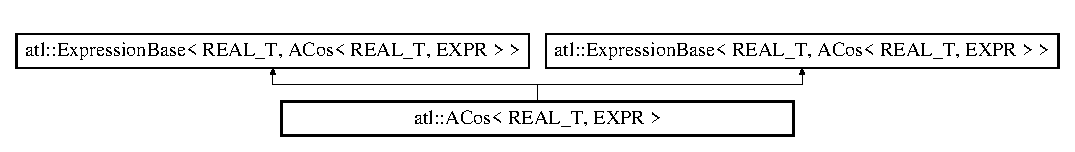
\includegraphics[height=1.595442cm]{structatl_1_1_a_cos}
\end{center}
\end{figure}
\subsection*{Public Types}
\begin{DoxyCompactItemize}
\item 
\hypertarget{structatl_1_1_a_cos_ac9971cad609b85379bbdf87f3199cce9}{typedef R\+E\+A\+L\+\_\+\+T {\bfseries B\+A\+S\+E\+\_\+\+T\+Y\+P\+E}}\label{structatl_1_1_a_cos_ac9971cad609b85379bbdf87f3199cce9}

\item 
\hypertarget{structatl_1_1_a_cos_ac9971cad609b85379bbdf87f3199cce9}{typedef R\+E\+A\+L\+\_\+\+T {\bfseries B\+A\+S\+E\+\_\+\+T\+Y\+P\+E}}\label{structatl_1_1_a_cos_ac9971cad609b85379bbdf87f3199cce9}

\end{DoxyCompactItemize}
\subsection*{Public Member Functions}
\begin{DoxyCompactItemize}
\item 
\hyperlink{structatl_1_1_a_cos_a574a9a5304ad7c90f7d2add7308a9510}{A\+Cos} (const \hyperlink{structatl_1_1_expression_base}{Expression\+Base}$<$ R\+E\+A\+L\+\_\+\+T, E\+X\+P\+R $>$ \&a)
\item 
const R\+E\+A\+L\+\_\+\+T \hyperlink{structatl_1_1_a_cos_ac88f1dd97b4cbccd7c40fb64efc57d3f}{Get\+Value} () const 
\item 
const R\+E\+A\+L\+\_\+\+T \hyperlink{structatl_1_1_a_cos_a444e9df0f5b21063bd332da73de6f23e}{Get\+Value} (size\+\_\+t i, size\+\_\+t j=0) const 
\item 
bool \hyperlink{structatl_1_1_a_cos_a8e94e5f51f01a559ea190d6fca8922e4}{Is\+Nonlinear} () const 
\item 
void \hyperlink{structatl_1_1_a_cos_a7c76416ec36329542e9fa9c8e61648c6}{Push\+Ids} (typename \hyperlink{structatl_1_1_stack_entry}{atl\+::\+Stack\+Entry}$<$ R\+E\+A\+L\+\_\+\+T $>$\+::vi\+\_\+storage \&ids) const 
\item 
void \hyperlink{structatl_1_1_a_cos_a5b882d4d0b3c5cd7195edc560cea5072}{Push\+Ids} (typename \hyperlink{structatl_1_1_stack_entry}{atl\+::\+Stack\+Entry}$<$ R\+E\+A\+L\+\_\+\+T $>$\+::vi\+\_\+storage \&ids, size\+\_\+t i, size\+\_\+t j=0) const 
\item 
const R\+E\+A\+L\+\_\+\+T \hyperlink{structatl_1_1_a_cos_a7df2e12cd867281e733d666097f576e3}{Evaluate\+Derivative} (uint32\+\_\+t x) const 
\item 
R\+E\+A\+L\+\_\+\+T \hyperlink{structatl_1_1_a_cos_a571db69e6082a154290e6aa4429ea8e3}{Evaluate\+Derivative} (uint32\+\_\+t x, uint32\+\_\+t y) const 
\item 
R\+E\+A\+L\+\_\+\+T \hyperlink{structatl_1_1_a_cos_a1080f087105145eeb86dbe4243108361}{Evaluate\+Derivative} (uint32\+\_\+t x, uint32\+\_\+t y, uint32\+\_\+t z) const 
\item 
const R\+E\+A\+L\+\_\+\+T \hyperlink{structatl_1_1_a_cos_a0b7efe188204ec1229c1849650d3b5c0}{Evaluate\+Derivative} (uint32\+\_\+t x, size\+\_\+t i, size\+\_\+t j=0) const 
\item 
R\+E\+A\+L\+\_\+\+T \hyperlink{structatl_1_1_a_cos_a03c9ced1e800232f5c0ee14c1ca61c89}{Evaluate\+Derivative} (uint32\+\_\+t x, uint32\+\_\+t y, size\+\_\+t i, size\+\_\+t j=0) const 
\item 
R\+E\+A\+L\+\_\+\+T \hyperlink{structatl_1_1_a_cos_aa454c4122ad33d32b098af408c51df21}{Evaluate\+Derivative} (uint32\+\_\+t x, uint32\+\_\+t y, uint32\+\_\+t z, size\+\_\+t i, size\+\_\+t j=0) const 
\item 
size\+\_\+t \hyperlink{structatl_1_1_a_cos_ae0af289491d112c68be1bd9d9e8f49fc}{Get\+Columns} () const 
\item 
size\+\_\+t \hyperlink{structatl_1_1_a_cos_a05cf14fff32555d4465cfff8fd103fa0}{Get\+Rows} () const 
\item 
bool \hyperlink{structatl_1_1_a_cos_a842f9d51e6afdba5c00fadfade2d2c69}{Is\+Scalar} () const 
\item 
const std\+::string \hyperlink{structatl_1_1_a_cos_a925347a32bc88e5167b911bdfe3459e9}{To\+Expression\+Template\+String} () const 
\item 
\hypertarget{structatl_1_1_a_cos_a574a9a5304ad7c90f7d2add7308a9510}{{\bfseries A\+Cos} (const \hyperlink{structatl_1_1_expression_base}{Expression\+Base}$<$ R\+E\+A\+L\+\_\+\+T, E\+X\+P\+R $>$ \&a)}\label{structatl_1_1_a_cos_a574a9a5304ad7c90f7d2add7308a9510}

\item 
\hypertarget{structatl_1_1_a_cos_ac88f1dd97b4cbccd7c40fb64efc57d3f}{const R\+E\+A\+L\+\_\+\+T {\bfseries Get\+Value} () const }\label{structatl_1_1_a_cos_ac88f1dd97b4cbccd7c40fb64efc57d3f}

\item 
\hypertarget{structatl_1_1_a_cos_a444e9df0f5b21063bd332da73de6f23e}{const R\+E\+A\+L\+\_\+\+T {\bfseries Get\+Value} (size\+\_\+t i, size\+\_\+t j=0) const }\label{structatl_1_1_a_cos_a444e9df0f5b21063bd332da73de6f23e}

\item 
\hypertarget{structatl_1_1_a_cos_a7c76416ec36329542e9fa9c8e61648c6}{void {\bfseries Push\+Ids} (typename \hyperlink{structatl_1_1_stack_entry}{atl\+::\+Stack\+Entry}$<$ R\+E\+A\+L\+\_\+\+T $>$\+::vi\+\_\+storage \&ids) const }\label{structatl_1_1_a_cos_a7c76416ec36329542e9fa9c8e61648c6}

\item 
\hypertarget{structatl_1_1_a_cos_a5b882d4d0b3c5cd7195edc560cea5072}{void {\bfseries Push\+Ids} (typename \hyperlink{structatl_1_1_stack_entry}{atl\+::\+Stack\+Entry}$<$ R\+E\+A\+L\+\_\+\+T $>$\+::vi\+\_\+storage \&ids, size\+\_\+t i, size\+\_\+t j=0) const }\label{structatl_1_1_a_cos_a5b882d4d0b3c5cd7195edc560cea5072}

\item 
\hypertarget{structatl_1_1_a_cos_ab0fc53c07b3cd29337759805c61a33b4}{const R\+E\+A\+L\+\_\+\+T {\bfseries Evaluate\+Derivative} (uint32\+\_\+t id) const }\label{structatl_1_1_a_cos_ab0fc53c07b3cd29337759805c61a33b4}

\item 
\hypertarget{structatl_1_1_a_cos_a64877d37ec3ddf545bfb22a3e704355d}{R\+E\+A\+L\+\_\+\+T {\bfseries Evaluate\+Derivative} (uint32\+\_\+t a, uint32\+\_\+t b) const }\label{structatl_1_1_a_cos_a64877d37ec3ddf545bfb22a3e704355d}

\item 
\hypertarget{structatl_1_1_a_cos_a1080f087105145eeb86dbe4243108361}{R\+E\+A\+L\+\_\+\+T {\bfseries Evaluate\+Derivative} (uint32\+\_\+t x, uint32\+\_\+t y, uint32\+\_\+t z) const }\label{structatl_1_1_a_cos_a1080f087105145eeb86dbe4243108361}

\item 
\hypertarget{structatl_1_1_a_cos_af5d4197ee310bef360a8470249999d01}{const R\+E\+A\+L\+\_\+\+T {\bfseries Evaluate\+Derivative} (uint32\+\_\+t id, size\+\_\+t i, size\+\_\+t j=0) const }\label{structatl_1_1_a_cos_af5d4197ee310bef360a8470249999d01}

\item 
\hypertarget{structatl_1_1_a_cos_af0a61f7d7dc6bcf090f442242297c1c3}{R\+E\+A\+L\+\_\+\+T {\bfseries Evaluate\+Derivative} (uint32\+\_\+t a, uint32\+\_\+t b, size\+\_\+t i, size\+\_\+t j=0) const }\label{structatl_1_1_a_cos_af0a61f7d7dc6bcf090f442242297c1c3}

\item 
\hypertarget{structatl_1_1_a_cos_aa454c4122ad33d32b098af408c51df21}{R\+E\+A\+L\+\_\+\+T {\bfseries Evaluate\+Derivative} (uint32\+\_\+t x, uint32\+\_\+t y, uint32\+\_\+t z, size\+\_\+t i, size\+\_\+t j=0) const }\label{structatl_1_1_a_cos_aa454c4122ad33d32b098af408c51df21}

\item 
\hypertarget{structatl_1_1_a_cos_ae0af289491d112c68be1bd9d9e8f49fc}{size\+\_\+t {\bfseries Get\+Columns} () const }\label{structatl_1_1_a_cos_ae0af289491d112c68be1bd9d9e8f49fc}

\item 
\hypertarget{structatl_1_1_a_cos_a05cf14fff32555d4465cfff8fd103fa0}{size\+\_\+t {\bfseries Get\+Rows} () const }\label{structatl_1_1_a_cos_a05cf14fff32555d4465cfff8fd103fa0}

\item 
\hypertarget{structatl_1_1_a_cos_a842f9d51e6afdba5c00fadfade2d2c69}{bool {\bfseries Is\+Scalar} () const }\label{structatl_1_1_a_cos_a842f9d51e6afdba5c00fadfade2d2c69}

\end{DoxyCompactItemize}
\subsection*{Public Attributes}
\begin{DoxyCompactItemize}
\item 
\hypertarget{structatl_1_1_a_cos_ae85789d9fea29c8516ca8a183961c2cc}{const E\+X\+P\+R \& {\bfseries expr\+\_\+m}}\label{structatl_1_1_a_cos_ae85789d9fea29c8516ca8a183961c2cc}

\end{DoxyCompactItemize}


\subsection{Detailed Description}
\subsubsection*{template$<$class R\+E\+A\+L\+\_\+\+T, class E\+X\+P\+R$>$struct atl\+::\+A\+Cos$<$ R\+E\+A\+L\+\_\+\+T, E\+X\+P\+R $>$}

Expression template to handle arccosine for variable or container expressions.

$ \arccos f(x,y) $

or

$ \arccos f_{i,j}(x,y) $ 

\subsection{Constructor \& Destructor Documentation}
\hypertarget{structatl_1_1_a_cos_a574a9a5304ad7c90f7d2add7308a9510}{\index{atl\+::\+A\+Cos@{atl\+::\+A\+Cos}!A\+Cos@{A\+Cos}}
\index{A\+Cos@{A\+Cos}!atl\+::\+A\+Cos@{atl\+::\+A\+Cos}}
\subsubsection[{A\+Cos}]{\setlength{\rightskip}{0pt plus 5cm}template$<$class R\+E\+A\+L\+\_\+\+T , class E\+X\+P\+R $>$ {\bf atl\+::\+A\+Cos}$<$ R\+E\+A\+L\+\_\+\+T, E\+X\+P\+R $>$\+::{\bf A\+Cos} (
\begin{DoxyParamCaption}
\item[{const {\bf Expression\+Base}$<$ R\+E\+A\+L\+\_\+\+T, E\+X\+P\+R $>$ \&}]{a}
\end{DoxyParamCaption}
)\hspace{0.3cm}{\ttfamily [inline]}}}\label{structatl_1_1_a_cos_a574a9a5304ad7c90f7d2add7308a9510}
Constructor


\begin{DoxyParams}{Parameters}
{\em a} & \\
\hline
\end{DoxyParams}


\subsection{Member Function Documentation}
\hypertarget{structatl_1_1_a_cos_a7df2e12cd867281e733d666097f576e3}{\index{atl\+::\+A\+Cos@{atl\+::\+A\+Cos}!Evaluate\+Derivative@{Evaluate\+Derivative}}
\index{Evaluate\+Derivative@{Evaluate\+Derivative}!atl\+::\+A\+Cos@{atl\+::\+A\+Cos}}
\subsubsection[{Evaluate\+Derivative}]{\setlength{\rightskip}{0pt plus 5cm}template$<$class R\+E\+A\+L\+\_\+\+T , class E\+X\+P\+R $>$ const R\+E\+A\+L\+\_\+\+T {\bf atl\+::\+A\+Cos}$<$ R\+E\+A\+L\+\_\+\+T, E\+X\+P\+R $>$\+::Evaluate\+Derivative (
\begin{DoxyParamCaption}
\item[{uint32\+\_\+t}]{x}
\end{DoxyParamCaption}
) const\hspace{0.3cm}{\ttfamily [inline]}}}\label{structatl_1_1_a_cos_a7df2e12cd867281e733d666097f576e3}
Evaluates the first-\/order derivative of this expression with respect to x.

$ -{{{{d}\over{d\,x}}\,f\left(x \right)}\over{\sqrt{1-f^2 \left(x \right)}}} $


\begin{DoxyParams}{Parameters}
{\em x} & \\
\hline
\end{DoxyParams}
\begin{DoxyReturn}{Returns}

\end{DoxyReturn}
\hypertarget{structatl_1_1_a_cos_a571db69e6082a154290e6aa4429ea8e3}{\index{atl\+::\+A\+Cos@{atl\+::\+A\+Cos}!Evaluate\+Derivative@{Evaluate\+Derivative}}
\index{Evaluate\+Derivative@{Evaluate\+Derivative}!atl\+::\+A\+Cos@{atl\+::\+A\+Cos}}
\subsubsection[{Evaluate\+Derivative}]{\setlength{\rightskip}{0pt plus 5cm}template$<$class R\+E\+A\+L\+\_\+\+T , class E\+X\+P\+R $>$ R\+E\+A\+L\+\_\+\+T {\bf atl\+::\+A\+Cos}$<$ R\+E\+A\+L\+\_\+\+T, E\+X\+P\+R $>$\+::Evaluate\+Derivative (
\begin{DoxyParamCaption}
\item[{uint32\+\_\+t}]{x, }
\item[{uint32\+\_\+t}]{y}
\end{DoxyParamCaption}
) const\hspace{0.3cm}{\ttfamily [inline]}}}\label{structatl_1_1_a_cos_a571db69e6082a154290e6aa4429ea8e3}
Evaluates the second-\/order mixed partial with respect to x and y.

$ -{{f\left(x , y\right)\,\left({{d}\over{d\,x}}\,f\left(x , y\right) \right)\,\left({{d}\over{d\,y}}\,f\left(x , y\right)\right)}\over{ \left(1-f^2\left(x , y\right)\right)^{{{3}\over{2}}}}}-{{{{d^2 }\over{d\,x\,d\,y}}\,f\left(x , y\right)}\over{\sqrt{1-f^2\left(x , y\right)}}} $


\begin{DoxyParams}{Parameters}
{\em x} & \\
\hline
{\em y} & \\
\hline
\end{DoxyParams}
\begin{DoxyReturn}{Returns}

\end{DoxyReturn}
\hypertarget{structatl_1_1_a_cos_a1080f087105145eeb86dbe4243108361}{\index{atl\+::\+A\+Cos@{atl\+::\+A\+Cos}!Evaluate\+Derivative@{Evaluate\+Derivative}}
\index{Evaluate\+Derivative@{Evaluate\+Derivative}!atl\+::\+A\+Cos@{atl\+::\+A\+Cos}}
\subsubsection[{Evaluate\+Derivative}]{\setlength{\rightskip}{0pt plus 5cm}template$<$class R\+E\+A\+L\+\_\+\+T , class E\+X\+P\+R $>$ R\+E\+A\+L\+\_\+\+T {\bf atl\+::\+A\+Cos}$<$ R\+E\+A\+L\+\_\+\+T, E\+X\+P\+R $>$\+::Evaluate\+Derivative (
\begin{DoxyParamCaption}
\item[{uint32\+\_\+t}]{x, }
\item[{uint32\+\_\+t}]{y, }
\item[{uint32\+\_\+t}]{z}
\end{DoxyParamCaption}
) const\hspace{0.3cm}{\ttfamily [inline]}}}\label{structatl_1_1_a_cos_a1080f087105145eeb86dbe4243108361}
Evaluates the third-\/order mixed partial with respect to x,y, and z.

$ -{{{{d}\over{d\,x}}\,f\left(x , y , z\right)\,\left({{d}\over{d\,y }}\,f\left(x , y , z\right)\right)\,\left({{d}\over{d\,z}}\,f\left(x , y , z\right)\right)}\over{\left(1-f^2\left(x , y , z\right) \right)^{{{3}\over{2}}}}}-{{3\,f^2\left(x , y , z\right)\,\left({{d }\over{d\,x}}\,f\left(x , y , z\right)\right)\,\left({{d}\over{d\,y }}\,f\left(x , y , z\right)\right)\,\left({{d}\over{d\,z}}\,f\left(x , y , z\right)\right)}\over{\left(1-f^2\left(x , y , z\right) \right)^{{{5}\over{2}}}}}-{{f\left(x , y , z\right)\,\left({{d^2 }\over{d\,x\,d\,y}}\,f\left(x , y , z\right)\right)\,\left({{d }\over{d\,z}}\,f\left(x , y , z\right)\right)}\over{\left(1-f^2 \left(x , y , z\right)\right)^{{{3}\over{2}}}}}- \\ {{f\left(x , y , z \right)\,\left({{d}\over{d\,x}}\,f\left(x , y , z\right)\right)\, \left({{d^2}\over{d\,y\,d\,z}}\,f\left(x , y , z\right)\right) }\over{\left(1-f^2\left(x , y , z\right)\right)^{{{3}\over{2}}}}}-{{ f\left(x , y , z\right)\,\left({{d^2}\over{d\,x\,d\,z}}\,f\left(x , y , z\right)\right)\,\left({{d}\over{d\,y}}\,f\left(x , y , z\right) \right)}\over{\left(1-f^2\left(x , y , z\right)\right)^{{{3}\over{2 }}}}}-{{{{d^3}\over{d\,x\,d\,y\,d\,z}}\,f\left(x , y , z\right) }\over{\sqrt{1-f^2\left(x , y , z\right)}}} $ 
\begin{DoxyParams}{Parameters}
{\em x} & \\
\hline
{\em y} & \\
\hline
{\em z} & \\
\hline
\end{DoxyParams}
\begin{DoxyReturn}{Returns}

\end{DoxyReturn}
\hypertarget{structatl_1_1_a_cos_a0b7efe188204ec1229c1849650d3b5c0}{\index{atl\+::\+A\+Cos@{atl\+::\+A\+Cos}!Evaluate\+Derivative@{Evaluate\+Derivative}}
\index{Evaluate\+Derivative@{Evaluate\+Derivative}!atl\+::\+A\+Cos@{atl\+::\+A\+Cos}}
\subsubsection[{Evaluate\+Derivative}]{\setlength{\rightskip}{0pt plus 5cm}template$<$class R\+E\+A\+L\+\_\+\+T , class E\+X\+P\+R $>$ const R\+E\+A\+L\+\_\+\+T {\bf atl\+::\+A\+Cos}$<$ R\+E\+A\+L\+\_\+\+T, E\+X\+P\+R $>$\+::Evaluate\+Derivative (
\begin{DoxyParamCaption}
\item[{uint32\+\_\+t}]{x, }
\item[{size\+\_\+t}]{i, }
\item[{size\+\_\+t}]{j = {\ttfamily 0}}
\end{DoxyParamCaption}
) const\hspace{0.3cm}{\ttfamily [inline]}}}\label{structatl_1_1_a_cos_a0b7efe188204ec1229c1849650d3b5c0}
Evaluates the first-\/order derivative of this expression with respect to x at index \{i,j\}.

$ -{{{{d}\over{d\,x}}\,f\left(x \right)}\over{\sqrt{1-f^2 \left(x \right)}}} $


\begin{DoxyParams}{Parameters}
{\em x} & \\
\hline
\end{DoxyParams}
\begin{DoxyReturn}{Returns}

\end{DoxyReturn}
\hypertarget{structatl_1_1_a_cos_a03c9ced1e800232f5c0ee14c1ca61c89}{\index{atl\+::\+A\+Cos@{atl\+::\+A\+Cos}!Evaluate\+Derivative@{Evaluate\+Derivative}}
\index{Evaluate\+Derivative@{Evaluate\+Derivative}!atl\+::\+A\+Cos@{atl\+::\+A\+Cos}}
\subsubsection[{Evaluate\+Derivative}]{\setlength{\rightskip}{0pt plus 5cm}template$<$class R\+E\+A\+L\+\_\+\+T , class E\+X\+P\+R $>$ R\+E\+A\+L\+\_\+\+T {\bf atl\+::\+A\+Cos}$<$ R\+E\+A\+L\+\_\+\+T, E\+X\+P\+R $>$\+::Evaluate\+Derivative (
\begin{DoxyParamCaption}
\item[{uint32\+\_\+t}]{x, }
\item[{uint32\+\_\+t}]{y, }
\item[{size\+\_\+t}]{i, }
\item[{size\+\_\+t}]{j = {\ttfamily 0}}
\end{DoxyParamCaption}
) const\hspace{0.3cm}{\ttfamily [inline]}}}\label{structatl_1_1_a_cos_a03c9ced1e800232f5c0ee14c1ca61c89}
Evaluates the second-\/order mixed partial with respect to x and y at index \{i,j\}.

$ -{{f_{i,j}(x,y)\,\left({{d}\over{d\,x}}\,f_{i,j}(x,y)\right)\, \left({{d}\over{d\,y}}\,f_{i,j}(x,y)\right)}\over{\left(1-f_{i,j}(x, y)^2\right)^{{{3}\over{2}}}}}-{{{{d^2}\over{d\,x\,d\,y}}\,f_{i,j}(x, y)}\over{\sqrt{1-f_{i,j}(x,y)^2}}} $ 
\begin{DoxyParams}{Parameters}
{\em x} & \\
\hline
{\em y} & \\
\hline
{\em i} & \\
\hline
{\em j} & \\
\hline
\end{DoxyParams}
\begin{DoxyReturn}{Returns}

\end{DoxyReturn}
\hypertarget{structatl_1_1_a_cos_aa454c4122ad33d32b098af408c51df21}{\index{atl\+::\+A\+Cos@{atl\+::\+A\+Cos}!Evaluate\+Derivative@{Evaluate\+Derivative}}
\index{Evaluate\+Derivative@{Evaluate\+Derivative}!atl\+::\+A\+Cos@{atl\+::\+A\+Cos}}
\subsubsection[{Evaluate\+Derivative}]{\setlength{\rightskip}{0pt plus 5cm}template$<$class R\+E\+A\+L\+\_\+\+T , class E\+X\+P\+R $>$ R\+E\+A\+L\+\_\+\+T {\bf atl\+::\+A\+Cos}$<$ R\+E\+A\+L\+\_\+\+T, E\+X\+P\+R $>$\+::Evaluate\+Derivative (
\begin{DoxyParamCaption}
\item[{uint32\+\_\+t}]{x, }
\item[{uint32\+\_\+t}]{y, }
\item[{uint32\+\_\+t}]{z, }
\item[{size\+\_\+t}]{i, }
\item[{size\+\_\+t}]{j = {\ttfamily 0}}
\end{DoxyParamCaption}
) const\hspace{0.3cm}{\ttfamily [inline]}}}\label{structatl_1_1_a_cos_aa454c4122ad33d32b098af408c51df21}
Evaluates the third-\/order mixed partial with respect to x,y, and z at index \{i,j\}.

$ -{{{{d}\over{d\,x}}\,f_{i,j}(x,y,z)\,\left({{d}\over{d\,y}}\,f_{i,j }(x,y,z)\right)\,\left({{d}\over{d\,z}}\,f_{i,j}(x,y,z)\right) }\over{\left(1-f_{i,j}(x,y,z)^2\right)^{{{3}\over{2}}}}}-{{3\,f_{i,j }(x,y,z)^2\,\left({{d}\over{d\,x}}\,f_{i,j}(x,y,z)\right)\,\left({{d }\over{d\,y}}\,f_{i,j}(x,y,z)\right)\,\left({{d}\over{d\,z}}\,f_{i,j }(x,y,z)\right)}\over{\left(1-f_{i,j}(x,y,z)^2\right)^{{{5}\over{2}} }}}-{{f_{i,j}(x,y,z)\,\left({{d^2}\over{d\,x\,d\,y}}\,f_{i,j}(x,y,z) \right)\,\left({{d}\over{d\,z}}\,f_{i,j}(x,y,z)\right)}\over{\left(1 -f_{i,j}(x,y,z)^2\right)^{{{3}\over{2}}}}}- \\ {{f_{i,j}(x,y,z)\,\left( {{d}\over{d\,x}}\,f_{i,j}(x,y,z)\right)\,\left({{d^2}\over{d\,y\,d\, z}}\,f_{i,j}(x,y,z)\right)}\over{\left(1-f_{i,j}(x,y,z)^2\right)^{{{ 3}\over{2}}}}}-{{f_{i,j}(x,y,z)\,\left({{d^2}\over{d\,x\,d\,z}}\,f_{ i,j}(x,y,z)\right)\,\left({{d}\over{d\,y}}\,f_{i,j}(x,y,z)\right) }\over{\left(1-f_{i,j}(x,y,z)^2\right)^{{{3}\over{2}}}}}-{{{{d^3 }\over{d\,x\,d\,y\,d\,z}}\,f_{i,j}(x,y,z)}\over{\sqrt{1-f_{i,j}(x,y, z)^2}}} $


\begin{DoxyParams}{Parameters}
{\em x} & \\
\hline
{\em y} & \\
\hline
{\em z} & \\
\hline
{\em i} & \\
\hline
{\em j} & \\
\hline
\end{DoxyParams}
\begin{DoxyReturn}{Returns}

\end{DoxyReturn}
\hypertarget{structatl_1_1_a_cos_ae0af289491d112c68be1bd9d9e8f49fc}{\index{atl\+::\+A\+Cos@{atl\+::\+A\+Cos}!Get\+Columns@{Get\+Columns}}
\index{Get\+Columns@{Get\+Columns}!atl\+::\+A\+Cos@{atl\+::\+A\+Cos}}
\subsubsection[{Get\+Columns}]{\setlength{\rightskip}{0pt plus 5cm}template$<$class R\+E\+A\+L\+\_\+\+T , class E\+X\+P\+R $>$ size\+\_\+t {\bf atl\+::\+A\+Cos}$<$ R\+E\+A\+L\+\_\+\+T, E\+X\+P\+R $>$\+::Get\+Columns (
\begin{DoxyParamCaption}
{}
\end{DoxyParamCaption}
) const\hspace{0.3cm}{\ttfamily [inline]}}}\label{structatl_1_1_a_cos_ae0af289491d112c68be1bd9d9e8f49fc}
Return the number of columns.

\begin{DoxyReturn}{Returns}

\end{DoxyReturn}
\hypertarget{structatl_1_1_a_cos_a05cf14fff32555d4465cfff8fd103fa0}{\index{atl\+::\+A\+Cos@{atl\+::\+A\+Cos}!Get\+Rows@{Get\+Rows}}
\index{Get\+Rows@{Get\+Rows}!atl\+::\+A\+Cos@{atl\+::\+A\+Cos}}
\subsubsection[{Get\+Rows}]{\setlength{\rightskip}{0pt plus 5cm}template$<$class R\+E\+A\+L\+\_\+\+T , class E\+X\+P\+R $>$ size\+\_\+t {\bf atl\+::\+A\+Cos}$<$ R\+E\+A\+L\+\_\+\+T, E\+X\+P\+R $>$\+::Get\+Rows (
\begin{DoxyParamCaption}
{}
\end{DoxyParamCaption}
) const\hspace{0.3cm}{\ttfamily [inline]}}}\label{structatl_1_1_a_cos_a05cf14fff32555d4465cfff8fd103fa0}
Return the number of rows.

\begin{DoxyReturn}{Returns}

\end{DoxyReturn}
\hypertarget{structatl_1_1_a_cos_ac88f1dd97b4cbccd7c40fb64efc57d3f}{\index{atl\+::\+A\+Cos@{atl\+::\+A\+Cos}!Get\+Value@{Get\+Value}}
\index{Get\+Value@{Get\+Value}!atl\+::\+A\+Cos@{atl\+::\+A\+Cos}}
\subsubsection[{Get\+Value}]{\setlength{\rightskip}{0pt plus 5cm}template$<$class R\+E\+A\+L\+\_\+\+T , class E\+X\+P\+R $>$ const R\+E\+A\+L\+\_\+\+T {\bf atl\+::\+A\+Cos}$<$ R\+E\+A\+L\+\_\+\+T, E\+X\+P\+R $>$\+::Get\+Value (
\begin{DoxyParamCaption}
{}
\end{DoxyParamCaption}
) const\hspace{0.3cm}{\ttfamily [inline]}}}\label{structatl_1_1_a_cos_ac88f1dd97b4cbccd7c40fb64efc57d3f}
Compute the arccosine of the expression.

\begin{DoxyReturn}{Returns}

\end{DoxyReturn}
\hypertarget{structatl_1_1_a_cos_a444e9df0f5b21063bd332da73de6f23e}{\index{atl\+::\+A\+Cos@{atl\+::\+A\+Cos}!Get\+Value@{Get\+Value}}
\index{Get\+Value@{Get\+Value}!atl\+::\+A\+Cos@{atl\+::\+A\+Cos}}
\subsubsection[{Get\+Value}]{\setlength{\rightskip}{0pt plus 5cm}template$<$class R\+E\+A\+L\+\_\+\+T , class E\+X\+P\+R $>$ const R\+E\+A\+L\+\_\+\+T {\bf atl\+::\+A\+Cos}$<$ R\+E\+A\+L\+\_\+\+T, E\+X\+P\+R $>$\+::Get\+Value (
\begin{DoxyParamCaption}
\item[{size\+\_\+t}]{i, }
\item[{size\+\_\+t}]{j = {\ttfamily 0}}
\end{DoxyParamCaption}
) const\hspace{0.3cm}{\ttfamily [inline]}}}\label{structatl_1_1_a_cos_a444e9df0f5b21063bd332da73de6f23e}
Compute the arccosine of the expression evaluated at index \{i,j\}.


\begin{DoxyParams}{Parameters}
{\em i} & \\
\hline
{\em j} & \\
\hline
\end{DoxyParams}
\begin{DoxyReturn}{Returns}

\end{DoxyReturn}
\hypertarget{structatl_1_1_a_cos_a8e94e5f51f01a559ea190d6fca8922e4}{\index{atl\+::\+A\+Cos@{atl\+::\+A\+Cos}!Is\+Nonlinear@{Is\+Nonlinear}}
\index{Is\+Nonlinear@{Is\+Nonlinear}!atl\+::\+A\+Cos@{atl\+::\+A\+Cos}}
\subsubsection[{Is\+Nonlinear}]{\setlength{\rightskip}{0pt plus 5cm}template$<$class R\+E\+A\+L\+\_\+\+T , class E\+X\+P\+R $>$ bool {\bf atl\+::\+A\+Cos}$<$ R\+E\+A\+L\+\_\+\+T, E\+X\+P\+R $>$\+::Is\+Nonlinear (
\begin{DoxyParamCaption}
{}
\end{DoxyParamCaption}
) const\hspace{0.3cm}{\ttfamily [inline]}}}\label{structatl_1_1_a_cos_a8e94e5f51f01a559ea190d6fca8922e4}
Returns true.

\begin{DoxyReturn}{Returns}

\end{DoxyReturn}
\hypertarget{structatl_1_1_a_cos_a842f9d51e6afdba5c00fadfade2d2c69}{\index{atl\+::\+A\+Cos@{atl\+::\+A\+Cos}!Is\+Scalar@{Is\+Scalar}}
\index{Is\+Scalar@{Is\+Scalar}!atl\+::\+A\+Cos@{atl\+::\+A\+Cos}}
\subsubsection[{Is\+Scalar}]{\setlength{\rightskip}{0pt plus 5cm}template$<$class R\+E\+A\+L\+\_\+\+T , class E\+X\+P\+R $>$ bool {\bf atl\+::\+A\+Cos}$<$ R\+E\+A\+L\+\_\+\+T, E\+X\+P\+R $>$\+::Is\+Scalar (
\begin{DoxyParamCaption}
{}
\end{DoxyParamCaption}
) const\hspace{0.3cm}{\ttfamily [inline]}}}\label{structatl_1_1_a_cos_a842f9d51e6afdba5c00fadfade2d2c69}
True if this expression is a scalar.

\begin{DoxyReturn}{Returns}

\end{DoxyReturn}
\hypertarget{structatl_1_1_a_cos_a7c76416ec36329542e9fa9c8e61648c6}{\index{atl\+::\+A\+Cos@{atl\+::\+A\+Cos}!Push\+Ids@{Push\+Ids}}
\index{Push\+Ids@{Push\+Ids}!atl\+::\+A\+Cos@{atl\+::\+A\+Cos}}
\subsubsection[{Push\+Ids}]{\setlength{\rightskip}{0pt plus 5cm}template$<$class R\+E\+A\+L\+\_\+\+T , class E\+X\+P\+R $>$ void {\bf atl\+::\+A\+Cos}$<$ R\+E\+A\+L\+\_\+\+T, E\+X\+P\+R $>$\+::Push\+Ids (
\begin{DoxyParamCaption}
\item[{typename {\bf atl\+::\+Stack\+Entry}$<$ R\+E\+A\+L\+\_\+\+T $>$\+::vi\+\_\+storage \&}]{ids}
\end{DoxyParamCaption}
) const\hspace{0.3cm}{\ttfamily [inline]}}}\label{structatl_1_1_a_cos_a7c76416ec36329542e9fa9c8e61648c6}
Push variable info into a set.


\begin{DoxyParams}{Parameters}
{\em ids} & \\
\hline
{\em i} & \\
\hline
{\em j} & \\
\hline
\end{DoxyParams}
\hypertarget{structatl_1_1_a_cos_a5b882d4d0b3c5cd7195edc560cea5072}{\index{atl\+::\+A\+Cos@{atl\+::\+A\+Cos}!Push\+Ids@{Push\+Ids}}
\index{Push\+Ids@{Push\+Ids}!atl\+::\+A\+Cos@{atl\+::\+A\+Cos}}
\subsubsection[{Push\+Ids}]{\setlength{\rightskip}{0pt plus 5cm}template$<$class R\+E\+A\+L\+\_\+\+T , class E\+X\+P\+R $>$ void {\bf atl\+::\+A\+Cos}$<$ R\+E\+A\+L\+\_\+\+T, E\+X\+P\+R $>$\+::Push\+Ids (
\begin{DoxyParamCaption}
\item[{typename {\bf atl\+::\+Stack\+Entry}$<$ R\+E\+A\+L\+\_\+\+T $>$\+::vi\+\_\+storage \&}]{ids, }
\item[{size\+\_\+t}]{i, }
\item[{size\+\_\+t}]{j = {\ttfamily 0}}
\end{DoxyParamCaption}
) const\hspace{0.3cm}{\ttfamily [inline]}}}\label{structatl_1_1_a_cos_a5b882d4d0b3c5cd7195edc560cea5072}
Push variable info into a set at index \{i,j\}.


\begin{DoxyParams}{Parameters}
{\em ids} & \\
\hline
{\em i} & \\
\hline
{\em j} & \\
\hline
\end{DoxyParams}
\hypertarget{structatl_1_1_a_cos_a925347a32bc88e5167b911bdfe3459e9}{\index{atl\+::\+A\+Cos@{atl\+::\+A\+Cos}!To\+Expression\+Template\+String@{To\+Expression\+Template\+String}}
\index{To\+Expression\+Template\+String@{To\+Expression\+Template\+String}!atl\+::\+A\+Cos@{atl\+::\+A\+Cos}}
\subsubsection[{To\+Expression\+Template\+String}]{\setlength{\rightskip}{0pt plus 5cm}template$<$class R\+E\+A\+L\+\_\+\+T , class E\+X\+P\+R $>$ const std\+::string {\bf atl\+::\+A\+Cos}$<$ R\+E\+A\+L\+\_\+\+T, E\+X\+P\+R $>$\+::To\+Expression\+Template\+String (
\begin{DoxyParamCaption}
{}
\end{DoxyParamCaption}
) const\hspace{0.3cm}{\ttfamily [inline]}}}\label{structatl_1_1_a_cos_a925347a32bc88e5167b911bdfe3459e9}
Create a string representation of this expression template. \begin{DoxyReturn}{Returns}

\end{DoxyReturn}


The documentation for this struct was generated from the following file\+:\begin{DoxyCompactItemize}
\item 
A\+Cos.\+hpp\end{DoxyCompactItemize}

\hypertarget{structatl_1_1_add}{\section{atl\+:\+:Add$<$ R\+E\+A\+L\+\_\+\+T, L\+H\+S, R\+H\+S $>$ Struct Template Reference}
\label{structatl_1_1_add}\index{atl\+::\+Add$<$ R\+E\+A\+L\+\_\+\+T, L\+H\+S, R\+H\+S $>$@{atl\+::\+Add$<$ R\+E\+A\+L\+\_\+\+T, L\+H\+S, R\+H\+S $>$}}
}


{\ttfamily \#include $<$Add.\+hpp$>$}

Inheritance diagram for atl\+:\+:Add$<$ R\+E\+A\+L\+\_\+\+T, L\+H\+S, R\+H\+S $>$\+:\begin{figure}[H]
\begin{center}
\leavevmode
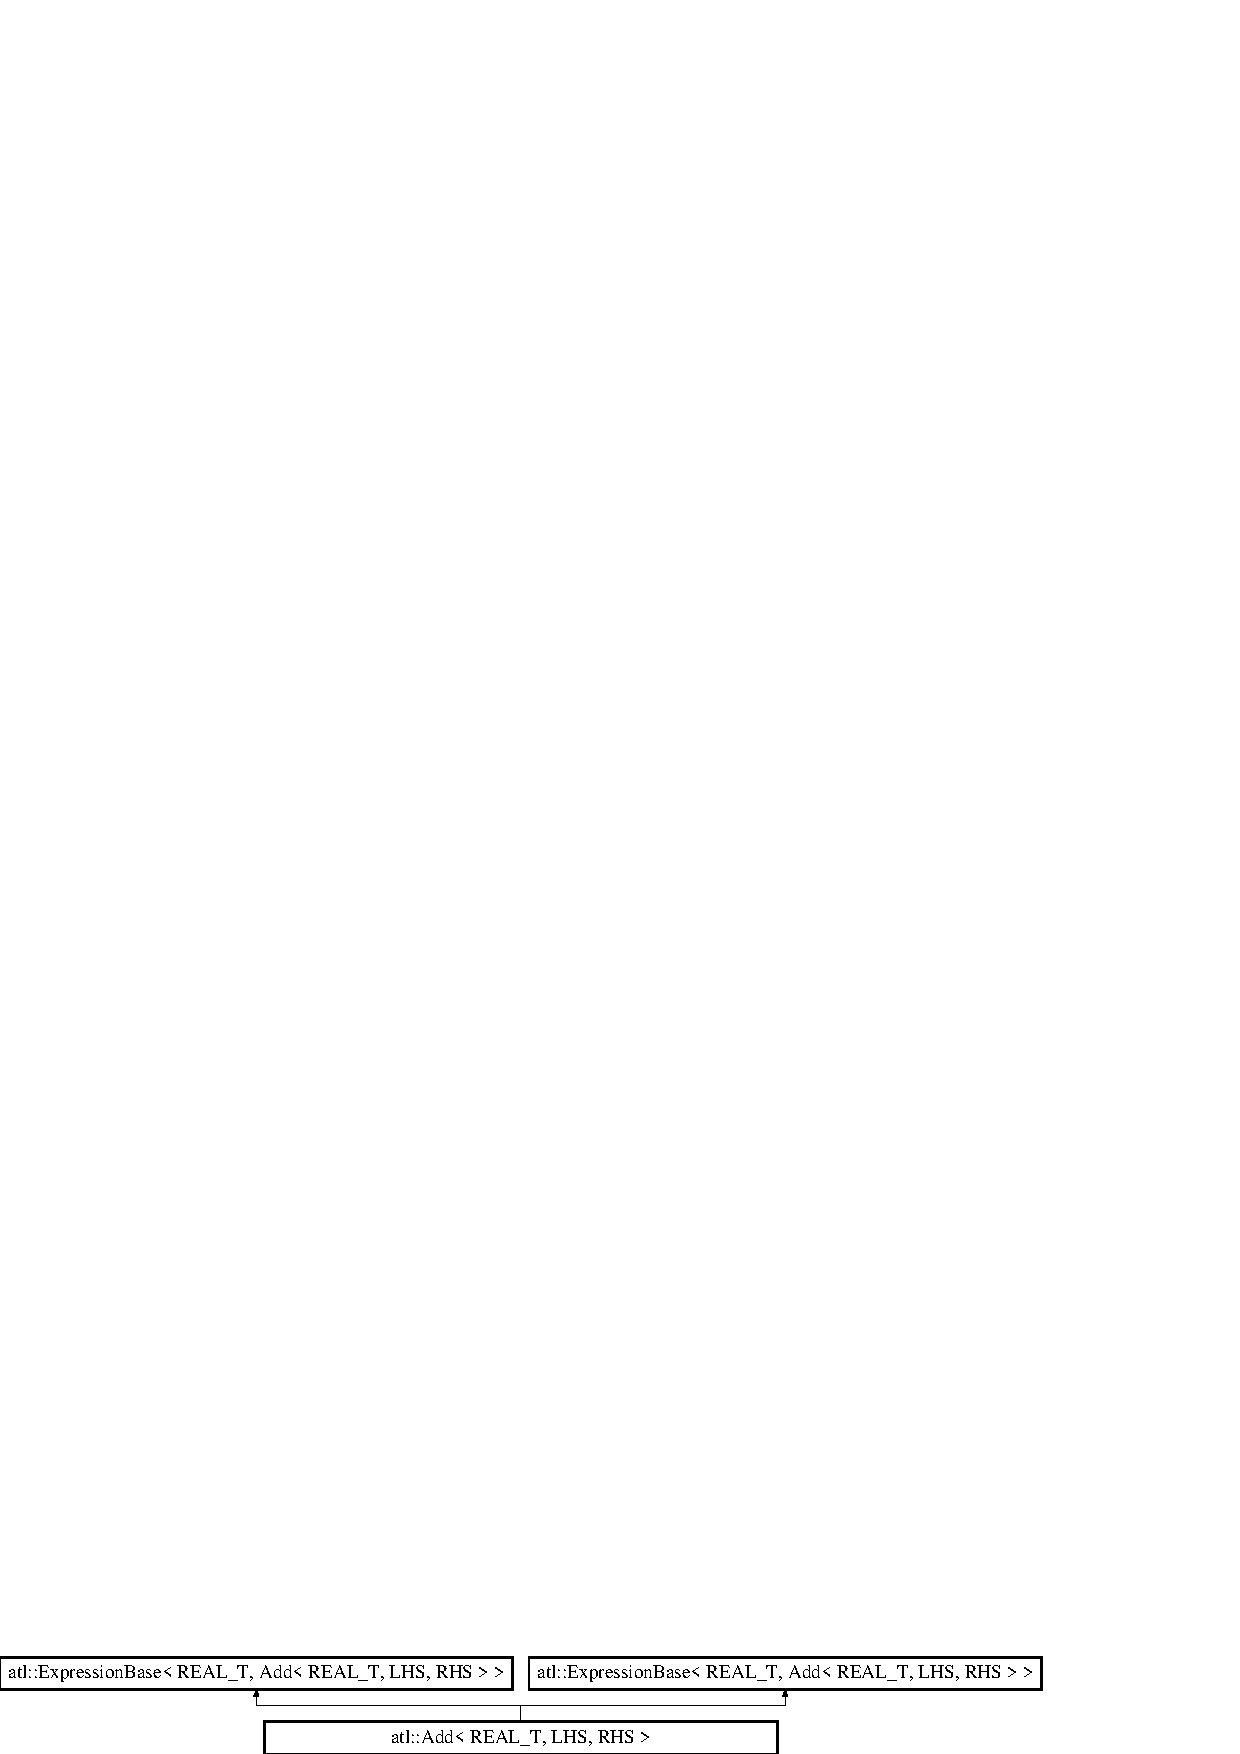
\includegraphics[height=1.521739cm]{structatl_1_1_add}
\end{center}
\end{figure}
\subsection*{Public Types}
\begin{DoxyCompactItemize}
\item 
\hypertarget{structatl_1_1_add_a1afac967194d1e503a20f9f56181833b}{typedef R\+E\+A\+L\+\_\+\+T {\bfseries B\+A\+S\+E\+\_\+\+T\+Y\+P\+E}}\label{structatl_1_1_add_a1afac967194d1e503a20f9f56181833b}

\item 
\hypertarget{structatl_1_1_add_a1afac967194d1e503a20f9f56181833b}{typedef R\+E\+A\+L\+\_\+\+T {\bfseries B\+A\+S\+E\+\_\+\+T\+Y\+P\+E}}\label{structatl_1_1_add_a1afac967194d1e503a20f9f56181833b}

\end{DoxyCompactItemize}
\subsection*{Public Member Functions}
\begin{DoxyCompactItemize}
\item 
\hyperlink{structatl_1_1_add_ae5adbfbec484c5c3d723961c507cceff}{Add} (const \hyperlink{structatl_1_1_expression_base}{Expression\+Base}$<$ R\+E\+A\+L\+\_\+\+T, L\+H\+S $>$ \&lhs, const \hyperlink{structatl_1_1_expression_base}{Expression\+Base}$<$ R\+E\+A\+L\+\_\+\+T, R\+H\+S $>$ \&rhs)
\item 
\hyperlink{structatl_1_1_add_a9e21358db0817bce5b9c8043defc1bb6}{Add} (const R\+E\+A\+L\+\_\+\+T \&lhs, const \hyperlink{structatl_1_1_expression_base}{Expression\+Base}$<$ R\+E\+A\+L\+\_\+\+T, R\+H\+S $>$ \&rhs)
\item 
\hyperlink{structatl_1_1_add_af3db07d03f92baf1728551fcda736ee2}{Add} (const \hyperlink{structatl_1_1_expression_base}{Expression\+Base}$<$ R\+E\+A\+L\+\_\+\+T, L\+H\+S $>$ \&lhs, const R\+E\+A\+L\+\_\+\+T \&rhs)
\item 
const R\+E\+A\+L\+\_\+\+T \hyperlink{structatl_1_1_add_a2c34acd36affef45b59ca3e2cbcf81aa}{Get\+Value} () const 
\item 
const R\+E\+A\+L\+\_\+\+T \hyperlink{structatl_1_1_add_a13e0ac75627c1747496f5aac500eb128}{Get\+Value} (size\+\_\+t i, size\+\_\+t j=0) const 
\item 
bool \hyperlink{structatl_1_1_add_a51e2295c5057bf50404e96949fb16912}{Is\+Nonlinear} () const 
\item 
void \hyperlink{structatl_1_1_add_a52a005a7a1dc1f38d77d6f142f3bea64}{Push\+Ids} (typename \hyperlink{structatl_1_1_stack_entry}{atl\+::\+Stack\+Entry}$<$ R\+E\+A\+L\+\_\+\+T $>$\+::vi\+\_\+storage \&ids) const 
\item 
void \hyperlink{structatl_1_1_add_a27cba5452b589a46fd4d6ab2abc1a7ea}{Push\+Ids} (typename \hyperlink{structatl_1_1_stack_entry}{atl\+::\+Stack\+Entry}$<$ R\+E\+A\+L\+\_\+\+T $>$\+::vi\+\_\+storage \&ids, size\+\_\+t i, size\+\_\+t j=0) const 
\item 
R\+E\+A\+L\+\_\+\+T \hyperlink{structatl_1_1_add_af08ab2cb8bc02783ac33756b91f5474d}{Evaluate\+Derivative} (uint32\+\_\+t x) const 
\item 
R\+E\+A\+L\+\_\+\+T \hyperlink{structatl_1_1_add_a156da3b3329007671fa005cfedbdf152}{Evaluate\+Derivative} (uint32\+\_\+t x, uint32\+\_\+t y) const 
\item 
R\+E\+A\+L\+\_\+\+T \hyperlink{structatl_1_1_add_ad6c38c9c3ef3bdb2eef2bc4b5832002f}{Evaluate\+Derivative} (uint32\+\_\+t x, uint32\+\_\+t y, uint32\+\_\+t z) const 
\item 
R\+E\+A\+L\+\_\+\+T \hyperlink{structatl_1_1_add_a2d787c2c79b11cda6707af72554595d2}{Evaluate\+Derivative} (uint32\+\_\+t x, size\+\_\+t i, size\+\_\+t j=0) const 
\item 
R\+E\+A\+L\+\_\+\+T \hyperlink{structatl_1_1_add_aaafbede3e546a91c5201a507a30384ef}{Evaluate\+Derivative} (uint32\+\_\+t x, uint32\+\_\+t y, size\+\_\+t i, size\+\_\+t j=0) const 
\item 
R\+E\+A\+L\+\_\+\+T \hyperlink{structatl_1_1_add_ad2ce1f0c07eba054a060c0c59f2e1e18}{Evaluate\+Derivative} (uint32\+\_\+t x, uint32\+\_\+t y, uint32\+\_\+t z, size\+\_\+t i, size\+\_\+t j=0) const 
\item 
size\+\_\+t \hyperlink{structatl_1_1_add_a221c4901b9658ab182b8be2e22554d96}{Get\+Columns} () const 
\item 
size\+\_\+t \hyperlink{structatl_1_1_add_a1786888970115c87917cc4e9d8571d4f}{Get\+Rows} () const 
\item 
bool \hyperlink{structatl_1_1_add_a88202aac52b67fab9f56026dff51339b}{Is\+Scalar} () const 
\item 
const std\+::string \hyperlink{structatl_1_1_add_a07527a08caf7d42751c3dc28fb71f0be}{To\+Expression\+Template\+String} () const 
\item 
\hypertarget{structatl_1_1_add_ae5adbfbec484c5c3d723961c507cceff}{{\bfseries Add} (const \hyperlink{structatl_1_1_expression_base}{Expression\+Base}$<$ R\+E\+A\+L\+\_\+\+T, L\+H\+S $>$ \&lhs, const \hyperlink{structatl_1_1_expression_base}{Expression\+Base}$<$ R\+E\+A\+L\+\_\+\+T, R\+H\+S $>$ \&rhs)}\label{structatl_1_1_add_ae5adbfbec484c5c3d723961c507cceff}

\item 
\hypertarget{structatl_1_1_add_a9e21358db0817bce5b9c8043defc1bb6}{{\bfseries Add} (const R\+E\+A\+L\+\_\+\+T \&lhs, const \hyperlink{structatl_1_1_expression_base}{Expression\+Base}$<$ R\+E\+A\+L\+\_\+\+T, R\+H\+S $>$ \&rhs)}\label{structatl_1_1_add_a9e21358db0817bce5b9c8043defc1bb6}

\item 
\hypertarget{structatl_1_1_add_af3db07d03f92baf1728551fcda736ee2}{{\bfseries Add} (const \hyperlink{structatl_1_1_expression_base}{Expression\+Base}$<$ R\+E\+A\+L\+\_\+\+T, L\+H\+S $>$ \&lhs, const R\+E\+A\+L\+\_\+\+T \&rhs)}\label{structatl_1_1_add_af3db07d03f92baf1728551fcda736ee2}

\item 
\hypertarget{structatl_1_1_add_a2c34acd36affef45b59ca3e2cbcf81aa}{const R\+E\+A\+L\+\_\+\+T {\bfseries Get\+Value} () const }\label{structatl_1_1_add_a2c34acd36affef45b59ca3e2cbcf81aa}

\item 
\hypertarget{structatl_1_1_add_a13e0ac75627c1747496f5aac500eb128}{const R\+E\+A\+L\+\_\+\+T {\bfseries Get\+Value} (size\+\_\+t i, size\+\_\+t j=0) const }\label{structatl_1_1_add_a13e0ac75627c1747496f5aac500eb128}

\item 
\hypertarget{structatl_1_1_add_a52a005a7a1dc1f38d77d6f142f3bea64}{void {\bfseries Push\+Ids} (typename \hyperlink{structatl_1_1_stack_entry}{atl\+::\+Stack\+Entry}$<$ R\+E\+A\+L\+\_\+\+T $>$\+::vi\+\_\+storage \&ids) const }\label{structatl_1_1_add_a52a005a7a1dc1f38d77d6f142f3bea64}

\item 
\hypertarget{structatl_1_1_add_a27cba5452b589a46fd4d6ab2abc1a7ea}{void {\bfseries Push\+Ids} (typename \hyperlink{structatl_1_1_stack_entry}{atl\+::\+Stack\+Entry}$<$ R\+E\+A\+L\+\_\+\+T $>$\+::vi\+\_\+storage \&ids, size\+\_\+t i, size\+\_\+t j=0) const }\label{structatl_1_1_add_a27cba5452b589a46fd4d6ab2abc1a7ea}

\item 
\hypertarget{structatl_1_1_add_a73a19f4ac2a363fcff0640f4132965d2}{R\+E\+A\+L\+\_\+\+T {\bfseries Evaluate\+Derivative} (uint32\+\_\+t a) const }\label{structatl_1_1_add_a73a19f4ac2a363fcff0640f4132965d2}

\item 
\hypertarget{structatl_1_1_add_a5bd2834df379dfb3afc945923b2fedd9}{R\+E\+A\+L\+\_\+\+T {\bfseries Evaluate\+Derivative} (uint32\+\_\+t a, uint32\+\_\+t b) const }\label{structatl_1_1_add_a5bd2834df379dfb3afc945923b2fedd9}

\item 
\hypertarget{structatl_1_1_add_ad6c38c9c3ef3bdb2eef2bc4b5832002f}{R\+E\+A\+L\+\_\+\+T {\bfseries Evaluate\+Derivative} (uint32\+\_\+t x, uint32\+\_\+t y, uint32\+\_\+t z) const }\label{structatl_1_1_add_ad6c38c9c3ef3bdb2eef2bc4b5832002f}

\item 
\hypertarget{structatl_1_1_add_a6762170a058b3e16760e6184f9a15759}{R\+E\+A\+L\+\_\+\+T {\bfseries Evaluate\+Derivative} (uint32\+\_\+t a, size\+\_\+t i, size\+\_\+t j=0) const }\label{structatl_1_1_add_a6762170a058b3e16760e6184f9a15759}

\item 
\hypertarget{structatl_1_1_add_a285b53b270ef1c8bda91fee83ae7ae19}{R\+E\+A\+L\+\_\+\+T {\bfseries Evaluate\+Derivative} (uint32\+\_\+t a, uint32\+\_\+t b, size\+\_\+t i, size\+\_\+t j=0) const }\label{structatl_1_1_add_a285b53b270ef1c8bda91fee83ae7ae19}

\item 
\hypertarget{structatl_1_1_add_ad2ce1f0c07eba054a060c0c59f2e1e18}{R\+E\+A\+L\+\_\+\+T {\bfseries Evaluate\+Derivative} (uint32\+\_\+t x, uint32\+\_\+t y, uint32\+\_\+t z, size\+\_\+t i, size\+\_\+t j=0) const }\label{structatl_1_1_add_ad2ce1f0c07eba054a060c0c59f2e1e18}

\item 
\hypertarget{structatl_1_1_add_a221c4901b9658ab182b8be2e22554d96}{size\+\_\+t {\bfseries Get\+Columns} () const }\label{structatl_1_1_add_a221c4901b9658ab182b8be2e22554d96}

\item 
\hypertarget{structatl_1_1_add_a1786888970115c87917cc4e9d8571d4f}{size\+\_\+t {\bfseries Get\+Rows} () const }\label{structatl_1_1_add_a1786888970115c87917cc4e9d8571d4f}

\item 
\hypertarget{structatl_1_1_add_a88202aac52b67fab9f56026dff51339b}{bool {\bfseries Is\+Scalar} () const }\label{structatl_1_1_add_a88202aac52b67fab9f56026dff51339b}

\end{DoxyCompactItemize}
\subsection*{Public Attributes}
\begin{DoxyCompactItemize}
\item 
\hypertarget{structatl_1_1_add_a46d0634fe0b197343c13de852b5b0cfa}{\hyperlink{structatl_1_1_real}{atl\+::\+Real}$<$ R\+E\+A\+L\+\_\+\+T $>$ {\bfseries real\+\_\+m}}\label{structatl_1_1_add_a46d0634fe0b197343c13de852b5b0cfa}

\item 
\hypertarget{structatl_1_1_add_aa2543240a578b7104a53ebf9d6c7ebdc}{const L\+H\+S \& {\bfseries lhs\+\_\+m}}\label{structatl_1_1_add_aa2543240a578b7104a53ebf9d6c7ebdc}

\item 
\hypertarget{structatl_1_1_add_aa2afd32dc41b6ab5effcf61b6c8e787c}{const R\+H\+S \& {\bfseries rhs\+\_\+m}}\label{structatl_1_1_add_aa2afd32dc41b6ab5effcf61b6c8e787c}

\item 
\hypertarget{structatl_1_1_add_a121a24d70ab887948e8b8a9d31197ac1}{R\+E\+A\+L\+\_\+\+T {\bfseries value\+\_\+m}}\label{structatl_1_1_add_a121a24d70ab887948e8b8a9d31197ac1}

\end{DoxyCompactItemize}


\subsection{Detailed Description}
\subsubsection*{template$<$class R\+E\+A\+L\+\_\+\+T, class L\+H\+S, class R\+H\+S$>$struct atl\+::\+Add$<$ R\+E\+A\+L\+\_\+\+T, L\+H\+S, R\+H\+S $>$}

Expression template to handle addition.

$ f(x) + g(x) $

or

$ f_{i,j}(x) + g_{i,j}(x) $ 

\subsection{Constructor \& Destructor Documentation}
\hypertarget{structatl_1_1_add_ae5adbfbec484c5c3d723961c507cceff}{\index{atl\+::\+Add@{atl\+::\+Add}!Add@{Add}}
\index{Add@{Add}!atl\+::\+Add@{atl\+::\+Add}}
\subsubsection[{Add}]{\setlength{\rightskip}{0pt plus 5cm}template$<$class R\+E\+A\+L\+\_\+\+T, class L\+H\+S , class R\+H\+S $>$ {\bf atl\+::\+Add}$<$ R\+E\+A\+L\+\_\+\+T, L\+H\+S, R\+H\+S $>$\+::{\bf Add} (
\begin{DoxyParamCaption}
\item[{const {\bf Expression\+Base}$<$ R\+E\+A\+L\+\_\+\+T, L\+H\+S $>$ \&}]{lhs, }
\item[{const {\bf Expression\+Base}$<$ R\+E\+A\+L\+\_\+\+T, R\+H\+S $>$ \&}]{rhs}
\end{DoxyParamCaption}
)\hspace{0.3cm}{\ttfamily [inline]}}}\label{structatl_1_1_add_ae5adbfbec484c5c3d723961c507cceff}
Constructor for two variable types.


\begin{DoxyParams}{Parameters}
{\em lhs} & \\
\hline
{\em rhs} & \\
\hline
\end{DoxyParams}
\hypertarget{structatl_1_1_add_a9e21358db0817bce5b9c8043defc1bb6}{\index{atl\+::\+Add@{atl\+::\+Add}!Add@{Add}}
\index{Add@{Add}!atl\+::\+Add@{atl\+::\+Add}}
\subsubsection[{Add}]{\setlength{\rightskip}{0pt plus 5cm}template$<$class R\+E\+A\+L\+\_\+\+T, class L\+H\+S , class R\+H\+S $>$ {\bf atl\+::\+Add}$<$ R\+E\+A\+L\+\_\+\+T, L\+H\+S, R\+H\+S $>$\+::{\bf Add} (
\begin{DoxyParamCaption}
\item[{const R\+E\+A\+L\+\_\+\+T \&}]{lhs, }
\item[{const {\bf Expression\+Base}$<$ R\+E\+A\+L\+\_\+\+T, R\+H\+S $>$ \&}]{rhs}
\end{DoxyParamCaption}
)\hspace{0.3cm}{\ttfamily [inline]}}}\label{structatl_1_1_add_a9e21358db0817bce5b9c8043defc1bb6}
Constructor for real plus variable type. \hypertarget{structatl_1_1_add_af3db07d03f92baf1728551fcda736ee2}{\index{atl\+::\+Add@{atl\+::\+Add}!Add@{Add}}
\index{Add@{Add}!atl\+::\+Add@{atl\+::\+Add}}
\subsubsection[{Add}]{\setlength{\rightskip}{0pt plus 5cm}template$<$class R\+E\+A\+L\+\_\+\+T, class L\+H\+S , class R\+H\+S $>$ {\bf atl\+::\+Add}$<$ R\+E\+A\+L\+\_\+\+T, L\+H\+S, R\+H\+S $>$\+::{\bf Add} (
\begin{DoxyParamCaption}
\item[{const {\bf Expression\+Base}$<$ R\+E\+A\+L\+\_\+\+T, L\+H\+S $>$ \&}]{lhs, }
\item[{const R\+E\+A\+L\+\_\+\+T \&}]{rhs}
\end{DoxyParamCaption}
)\hspace{0.3cm}{\ttfamily [inline]}}}\label{structatl_1_1_add_af3db07d03f92baf1728551fcda736ee2}
Constructor for variable plus real type. 
\begin{DoxyParams}{Parameters}
{\em lhs} & \\
\hline
{\em rhs} & \\
\hline
\end{DoxyParams}


\subsection{Member Function Documentation}
\hypertarget{structatl_1_1_add_af08ab2cb8bc02783ac33756b91f5474d}{\index{atl\+::\+Add@{atl\+::\+Add}!Evaluate\+Derivative@{Evaluate\+Derivative}}
\index{Evaluate\+Derivative@{Evaluate\+Derivative}!atl\+::\+Add@{atl\+::\+Add}}
\subsubsection[{Evaluate\+Derivative}]{\setlength{\rightskip}{0pt plus 5cm}template$<$class R\+E\+A\+L\+\_\+\+T, class L\+H\+S , class R\+H\+S $>$ R\+E\+A\+L\+\_\+\+T {\bf atl\+::\+Add}$<$ R\+E\+A\+L\+\_\+\+T, L\+H\+S, R\+H\+S $>$\+::Evaluate\+Derivative (
\begin{DoxyParamCaption}
\item[{uint32\+\_\+t}]{x}
\end{DoxyParamCaption}
) const\hspace{0.3cm}{\ttfamily [inline]}}}\label{structatl_1_1_add_af08ab2cb8bc02783ac33756b91f5474d}
Evaluates the first-\/order derivative with respect to x.

$ {{d}\over{d\,x}}\,g\left(x\right)+{{d}\over{d\,x}}\,f\left(x\right) $


\begin{DoxyParams}{Parameters}
{\em x} & \\
\hline
\end{DoxyParams}
\begin{DoxyReturn}{Returns}

\end{DoxyReturn}
\hypertarget{structatl_1_1_add_a156da3b3329007671fa005cfedbdf152}{\index{atl\+::\+Add@{atl\+::\+Add}!Evaluate\+Derivative@{Evaluate\+Derivative}}
\index{Evaluate\+Derivative@{Evaluate\+Derivative}!atl\+::\+Add@{atl\+::\+Add}}
\subsubsection[{Evaluate\+Derivative}]{\setlength{\rightskip}{0pt plus 5cm}template$<$class R\+E\+A\+L\+\_\+\+T, class L\+H\+S , class R\+H\+S $>$ R\+E\+A\+L\+\_\+\+T {\bf atl\+::\+Add}$<$ R\+E\+A\+L\+\_\+\+T, L\+H\+S, R\+H\+S $>$\+::Evaluate\+Derivative (
\begin{DoxyParamCaption}
\item[{uint32\+\_\+t}]{x, }
\item[{uint32\+\_\+t}]{y}
\end{DoxyParamCaption}
) const\hspace{0.3cm}{\ttfamily [inline]}}}\label{structatl_1_1_add_a156da3b3329007671fa005cfedbdf152}
Evaluates the second-\/order derivative with respect to x and y.

$ {{d^2}\over{d\,x\,d\,y}}\,g\left(x , y\right)+{{d^2}\over{d\,x\,d\, y}}\,f\left(x , y\right) $ 
\begin{DoxyParams}{Parameters}
{\em x} & \\
\hline
{\em y} & \\
\hline
\end{DoxyParams}
\begin{DoxyReturn}{Returns}

\end{DoxyReturn}
\hypertarget{structatl_1_1_add_ad6c38c9c3ef3bdb2eef2bc4b5832002f}{\index{atl\+::\+Add@{atl\+::\+Add}!Evaluate\+Derivative@{Evaluate\+Derivative}}
\index{Evaluate\+Derivative@{Evaluate\+Derivative}!atl\+::\+Add@{atl\+::\+Add}}
\subsubsection[{Evaluate\+Derivative}]{\setlength{\rightskip}{0pt plus 5cm}template$<$class R\+E\+A\+L\+\_\+\+T, class L\+H\+S , class R\+H\+S $>$ R\+E\+A\+L\+\_\+\+T {\bf atl\+::\+Add}$<$ R\+E\+A\+L\+\_\+\+T, L\+H\+S, R\+H\+S $>$\+::Evaluate\+Derivative (
\begin{DoxyParamCaption}
\item[{uint32\+\_\+t}]{x, }
\item[{uint32\+\_\+t}]{y, }
\item[{uint32\+\_\+t}]{z}
\end{DoxyParamCaption}
) const\hspace{0.3cm}{\ttfamily [inline]}}}\label{structatl_1_1_add_ad6c38c9c3ef3bdb2eef2bc4b5832002f}
Evaluates the third-\/order derivative with respect to x, y, and z.

$ {{d^3}\over{d\,x\,d\,y\,d\,z}}\,g\left(x , y , z\right)+{{d^3 }\over{d\,x\,d\,y\,d\,z}}\,f\left(x , y , z\right) $ 
\begin{DoxyParams}{Parameters}
{\em x} & \\
\hline
{\em y} & \\
\hline
{\em z} & \\
\hline
\end{DoxyParams}
\begin{DoxyReturn}{Returns}

\end{DoxyReturn}
\hypertarget{structatl_1_1_add_a2d787c2c79b11cda6707af72554595d2}{\index{atl\+::\+Add@{atl\+::\+Add}!Evaluate\+Derivative@{Evaluate\+Derivative}}
\index{Evaluate\+Derivative@{Evaluate\+Derivative}!atl\+::\+Add@{atl\+::\+Add}}
\subsubsection[{Evaluate\+Derivative}]{\setlength{\rightskip}{0pt plus 5cm}template$<$class R\+E\+A\+L\+\_\+\+T, class L\+H\+S , class R\+H\+S $>$ R\+E\+A\+L\+\_\+\+T {\bf atl\+::\+Add}$<$ R\+E\+A\+L\+\_\+\+T, L\+H\+S, R\+H\+S $>$\+::Evaluate\+Derivative (
\begin{DoxyParamCaption}
\item[{uint32\+\_\+t}]{x, }
\item[{size\+\_\+t}]{i, }
\item[{size\+\_\+t}]{j = {\ttfamily 0}}
\end{DoxyParamCaption}
) const\hspace{0.3cm}{\ttfamily [inline]}}}\label{structatl_1_1_add_a2d787c2c79b11cda6707af72554595d2}
Evaluates the first-\/order derivative of this expression with respect to x at index \{i,j\}.


\begin{DoxyParams}{Parameters}
{\em a} & \\
\hline
{\em i} & \\
\hline
{\em j} & \\
\hline
\end{DoxyParams}
\begin{DoxyReturn}{Returns}

\end{DoxyReturn}
\hypertarget{structatl_1_1_add_aaafbede3e546a91c5201a507a30384ef}{\index{atl\+::\+Add@{atl\+::\+Add}!Evaluate\+Derivative@{Evaluate\+Derivative}}
\index{Evaluate\+Derivative@{Evaluate\+Derivative}!atl\+::\+Add@{atl\+::\+Add}}
\subsubsection[{Evaluate\+Derivative}]{\setlength{\rightskip}{0pt plus 5cm}template$<$class R\+E\+A\+L\+\_\+\+T, class L\+H\+S , class R\+H\+S $>$ R\+E\+A\+L\+\_\+\+T {\bf atl\+::\+Add}$<$ R\+E\+A\+L\+\_\+\+T, L\+H\+S, R\+H\+S $>$\+::Evaluate\+Derivative (
\begin{DoxyParamCaption}
\item[{uint32\+\_\+t}]{x, }
\item[{uint32\+\_\+t}]{y, }
\item[{size\+\_\+t}]{i, }
\item[{size\+\_\+t}]{j = {\ttfamily 0}}
\end{DoxyParamCaption}
) const\hspace{0.3cm}{\ttfamily [inline]}}}\label{structatl_1_1_add_aaafbede3e546a91c5201a507a30384ef}
Evaluates the second-\/order derivative of this expression with respect to x at index \{i,j\}. 
\begin{DoxyParams}{Parameters}
{\em x} & \\
\hline
{\em y} & \\
\hline
{\em i} & \\
\hline
{\em j} & \\
\hline
\end{DoxyParams}
\begin{DoxyReturn}{Returns}

\end{DoxyReturn}
\hypertarget{structatl_1_1_add_ad2ce1f0c07eba054a060c0c59f2e1e18}{\index{atl\+::\+Add@{atl\+::\+Add}!Evaluate\+Derivative@{Evaluate\+Derivative}}
\index{Evaluate\+Derivative@{Evaluate\+Derivative}!atl\+::\+Add@{atl\+::\+Add}}
\subsubsection[{Evaluate\+Derivative}]{\setlength{\rightskip}{0pt plus 5cm}template$<$class R\+E\+A\+L\+\_\+\+T, class L\+H\+S , class R\+H\+S $>$ R\+E\+A\+L\+\_\+\+T {\bf atl\+::\+Add}$<$ R\+E\+A\+L\+\_\+\+T, L\+H\+S, R\+H\+S $>$\+::Evaluate\+Derivative (
\begin{DoxyParamCaption}
\item[{uint32\+\_\+t}]{x, }
\item[{uint32\+\_\+t}]{y, }
\item[{uint32\+\_\+t}]{z, }
\item[{size\+\_\+t}]{i, }
\item[{size\+\_\+t}]{j = {\ttfamily 0}}
\end{DoxyParamCaption}
) const\hspace{0.3cm}{\ttfamily [inline]}}}\label{structatl_1_1_add_ad2ce1f0c07eba054a060c0c59f2e1e18}
Evaluates the second-\/order derivative of this expression with respect to x at index \{i,j\}. 
\begin{DoxyParams}{Parameters}
{\em x} & \\
\hline
{\em y} & \\
\hline
{\em z} & \\
\hline
{\em i} & \\
\hline
{\em j} & \\
\hline
\end{DoxyParams}
\begin{DoxyReturn}{Returns}

\end{DoxyReturn}
\hypertarget{structatl_1_1_add_a221c4901b9658ab182b8be2e22554d96}{\index{atl\+::\+Add@{atl\+::\+Add}!Get\+Columns@{Get\+Columns}}
\index{Get\+Columns@{Get\+Columns}!atl\+::\+Add@{atl\+::\+Add}}
\subsubsection[{Get\+Columns}]{\setlength{\rightskip}{0pt plus 5cm}template$<$class R\+E\+A\+L\+\_\+\+T, class L\+H\+S , class R\+H\+S $>$ size\+\_\+t {\bf atl\+::\+Add}$<$ R\+E\+A\+L\+\_\+\+T, L\+H\+S, R\+H\+S $>$\+::Get\+Columns (
\begin{DoxyParamCaption}
{}
\end{DoxyParamCaption}
) const\hspace{0.3cm}{\ttfamily [inline]}}}\label{structatl_1_1_add_a221c4901b9658ab182b8be2e22554d96}
Return the number of columns.

\begin{DoxyReturn}{Returns}

\end{DoxyReturn}
\hypertarget{structatl_1_1_add_a1786888970115c87917cc4e9d8571d4f}{\index{atl\+::\+Add@{atl\+::\+Add}!Get\+Rows@{Get\+Rows}}
\index{Get\+Rows@{Get\+Rows}!atl\+::\+Add@{atl\+::\+Add}}
\subsubsection[{Get\+Rows}]{\setlength{\rightskip}{0pt plus 5cm}template$<$class R\+E\+A\+L\+\_\+\+T, class L\+H\+S , class R\+H\+S $>$ size\+\_\+t {\bf atl\+::\+Add}$<$ R\+E\+A\+L\+\_\+\+T, L\+H\+S, R\+H\+S $>$\+::Get\+Rows (
\begin{DoxyParamCaption}
{}
\end{DoxyParamCaption}
) const\hspace{0.3cm}{\ttfamily [inline]}}}\label{structatl_1_1_add_a1786888970115c87917cc4e9d8571d4f}
Return the number of rows.

\begin{DoxyReturn}{Returns}

\end{DoxyReturn}
\hypertarget{structatl_1_1_add_a2c34acd36affef45b59ca3e2cbcf81aa}{\index{atl\+::\+Add@{atl\+::\+Add}!Get\+Value@{Get\+Value}}
\index{Get\+Value@{Get\+Value}!atl\+::\+Add@{atl\+::\+Add}}
\subsubsection[{Get\+Value}]{\setlength{\rightskip}{0pt plus 5cm}template$<$class R\+E\+A\+L\+\_\+\+T, class L\+H\+S , class R\+H\+S $>$ const R\+E\+A\+L\+\_\+\+T {\bf atl\+::\+Add}$<$ R\+E\+A\+L\+\_\+\+T, L\+H\+S, R\+H\+S $>$\+::Get\+Value (
\begin{DoxyParamCaption}
{}
\end{DoxyParamCaption}
) const\hspace{0.3cm}{\ttfamily [inline]}}}\label{structatl_1_1_add_a2c34acd36affef45b59ca3e2cbcf81aa}
Compute the addition of the lhs and rhs expressions.

\begin{DoxyReturn}{Returns}

\end{DoxyReturn}
\hypertarget{structatl_1_1_add_a13e0ac75627c1747496f5aac500eb128}{\index{atl\+::\+Add@{atl\+::\+Add}!Get\+Value@{Get\+Value}}
\index{Get\+Value@{Get\+Value}!atl\+::\+Add@{atl\+::\+Add}}
\subsubsection[{Get\+Value}]{\setlength{\rightskip}{0pt plus 5cm}template$<$class R\+E\+A\+L\+\_\+\+T, class L\+H\+S , class R\+H\+S $>$ const R\+E\+A\+L\+\_\+\+T {\bf atl\+::\+Add}$<$ R\+E\+A\+L\+\_\+\+T, L\+H\+S, R\+H\+S $>$\+::Get\+Value (
\begin{DoxyParamCaption}
\item[{size\+\_\+t}]{i, }
\item[{size\+\_\+t}]{j = {\ttfamily 0}}
\end{DoxyParamCaption}
) const\hspace{0.3cm}{\ttfamily [inline]}}}\label{structatl_1_1_add_a13e0ac75627c1747496f5aac500eb128}
Compute the addition of the lhs and rhs expressions at index \{i,j\}.

\begin{DoxyReturn}{Returns}

\end{DoxyReturn}
\hypertarget{structatl_1_1_add_a51e2295c5057bf50404e96949fb16912}{\index{atl\+::\+Add@{atl\+::\+Add}!Is\+Nonlinear@{Is\+Nonlinear}}
\index{Is\+Nonlinear@{Is\+Nonlinear}!atl\+::\+Add@{atl\+::\+Add}}
\subsubsection[{Is\+Nonlinear}]{\setlength{\rightskip}{0pt plus 5cm}template$<$class R\+E\+A\+L\+\_\+\+T, class L\+H\+S , class R\+H\+S $>$ bool {\bf atl\+::\+Add}$<$ R\+E\+A\+L\+\_\+\+T, L\+H\+S, R\+H\+S $>$\+::Is\+Nonlinear (
\begin{DoxyParamCaption}
{}
\end{DoxyParamCaption}
) const\hspace{0.3cm}{\ttfamily [inline]}}}\label{structatl_1_1_add_a51e2295c5057bf50404e96949fb16912}
Returns true if the left or right side is nonlinear, else false. \begin{DoxyReturn}{Returns}

\end{DoxyReturn}
\hypertarget{structatl_1_1_add_a88202aac52b67fab9f56026dff51339b}{\index{atl\+::\+Add@{atl\+::\+Add}!Is\+Scalar@{Is\+Scalar}}
\index{Is\+Scalar@{Is\+Scalar}!atl\+::\+Add@{atl\+::\+Add}}
\subsubsection[{Is\+Scalar}]{\setlength{\rightskip}{0pt plus 5cm}template$<$class R\+E\+A\+L\+\_\+\+T, class L\+H\+S , class R\+H\+S $>$ bool {\bf atl\+::\+Add}$<$ R\+E\+A\+L\+\_\+\+T, L\+H\+S, R\+H\+S $>$\+::Is\+Scalar (
\begin{DoxyParamCaption}
{}
\end{DoxyParamCaption}
) const\hspace{0.3cm}{\ttfamily [inline]}}}\label{structatl_1_1_add_a88202aac52b67fab9f56026dff51339b}
True if the expression is a scalar. \begin{DoxyReturn}{Returns}

\end{DoxyReturn}
\hypertarget{structatl_1_1_add_a52a005a7a1dc1f38d77d6f142f3bea64}{\index{atl\+::\+Add@{atl\+::\+Add}!Push\+Ids@{Push\+Ids}}
\index{Push\+Ids@{Push\+Ids}!atl\+::\+Add@{atl\+::\+Add}}
\subsubsection[{Push\+Ids}]{\setlength{\rightskip}{0pt plus 5cm}template$<$class R\+E\+A\+L\+\_\+\+T, class L\+H\+S , class R\+H\+S $>$ void {\bf atl\+::\+Add}$<$ R\+E\+A\+L\+\_\+\+T, L\+H\+S, R\+H\+S $>$\+::Push\+Ids (
\begin{DoxyParamCaption}
\item[{typename {\bf atl\+::\+Stack\+Entry}$<$ R\+E\+A\+L\+\_\+\+T $>$\+::vi\+\_\+storage \&}]{ids}
\end{DoxyParamCaption}
) const\hspace{0.3cm}{\ttfamily [inline]}}}\label{structatl_1_1_add_a52a005a7a1dc1f38d77d6f142f3bea64}
Push variable info into a set.


\begin{DoxyParams}{Parameters}
{\em ids} & \\
\hline
\end{DoxyParams}
\hypertarget{structatl_1_1_add_a27cba5452b589a46fd4d6ab2abc1a7ea}{\index{atl\+::\+Add@{atl\+::\+Add}!Push\+Ids@{Push\+Ids}}
\index{Push\+Ids@{Push\+Ids}!atl\+::\+Add@{atl\+::\+Add}}
\subsubsection[{Push\+Ids}]{\setlength{\rightskip}{0pt plus 5cm}template$<$class R\+E\+A\+L\+\_\+\+T, class L\+H\+S , class R\+H\+S $>$ void {\bf atl\+::\+Add}$<$ R\+E\+A\+L\+\_\+\+T, L\+H\+S, R\+H\+S $>$\+::Push\+Ids (
\begin{DoxyParamCaption}
\item[{typename {\bf atl\+::\+Stack\+Entry}$<$ R\+E\+A\+L\+\_\+\+T $>$\+::vi\+\_\+storage \&}]{ids, }
\item[{size\+\_\+t}]{i, }
\item[{size\+\_\+t}]{j = {\ttfamily 0}}
\end{DoxyParamCaption}
) const\hspace{0.3cm}{\ttfamily [inline]}}}\label{structatl_1_1_add_a27cba5452b589a46fd4d6ab2abc1a7ea}
Push variable info into a set at index \{i,j\}.


\begin{DoxyParams}{Parameters}
{\em ids} & \\
\hline
{\em i} & \\
\hline
{\em j} & \\
\hline
\end{DoxyParams}
\hypertarget{structatl_1_1_add_a07527a08caf7d42751c3dc28fb71f0be}{\index{atl\+::\+Add@{atl\+::\+Add}!To\+Expression\+Template\+String@{To\+Expression\+Template\+String}}
\index{To\+Expression\+Template\+String@{To\+Expression\+Template\+String}!atl\+::\+Add@{atl\+::\+Add}}
\subsubsection[{To\+Expression\+Template\+String}]{\setlength{\rightskip}{0pt plus 5cm}template$<$class R\+E\+A\+L\+\_\+\+T, class L\+H\+S , class R\+H\+S $>$ const std\+::string {\bf atl\+::\+Add}$<$ R\+E\+A\+L\+\_\+\+T, L\+H\+S, R\+H\+S $>$\+::To\+Expression\+Template\+String (
\begin{DoxyParamCaption}
{}
\end{DoxyParamCaption}
) const\hspace{0.3cm}{\ttfamily [inline]}}}\label{structatl_1_1_add_a07527a08caf7d42751c3dc28fb71f0be}
Create a string representation of this expression template. \begin{DoxyReturn}{Returns}

\end{DoxyReturn}


The documentation for this struct was generated from the following file\+:\begin{DoxyCompactItemize}
\item 
Add.\+hpp\end{DoxyCompactItemize}

\hypertarget{unionanchor}{\section{anchor Union Reference}
\label{unionanchor}\index{anchor@{anchor}}
}
\subsection*{Public Attributes}
\begin{DoxyCompactItemize}
\item 
\hypertarget{unionanchor_a1da07b5c583e172230b98ce2f9d02207}{\begin{tabbing}
xx\=xx\=xx\=xx\=xx\=xx\=xx\=xx\=xx\=\kill
struct \{\\
\>unsigned {\bfseries head}: 7\\
\>unsigned {\bfseries count}: 7\\
\>unsigned {\bfseries active}: 1\\
\>unsigned {\bfseries valid}: 1\\
\>anchorsize\_t {\bfseries tag}: 8 $\ast$ sizeof (anchorsize\_t) -\/ 16\\
\} {\bfseries sep}}\label{unionanchor_a1da07b5c583e172230b98ce2f9d02207}
\\

\end{tabbing}\item 
\hypertarget{unionanchor_a57781a3ec5d817fc67d4bfba5a7aaee6}{anchorsize\+\_\+t {\bfseries all}}\label{unionanchor_a57781a3ec5d817fc67d4bfba5a7aaee6}

\item 
\hypertarget{unionanchor_af545f527dd057d25fb5d4c09e8ed876e}{\begin{tabbing}
xx\=xx\=xx\=xx\=xx\=xx\=xx\=xx\=xx\=\kill
struct \{\\
\>unsigned {\bfseries head}: 7\\
\>unsigned {\bfseries count}: 7\\
\>unsigned {\bfseries active}: 1\\
\>unsigned {\bfseries valid}: 1\\
\>anchorsize\_t {\bfseries tag}: 8 $\ast$ sizeof (anchorsize\_t) -\/ 16\\
\} {\bfseries sep}}\label{unionanchor_af545f527dd057d25fb5d4c09e8ed876e}
\\

\end{tabbing}\end{DoxyCompactItemize}


The documentation for this union was generated from the following file\+:\begin{DoxyCompactItemize}
\item 
A\+T\+L2/clfmalloc.\+h\end{DoxyCompactItemize}

\hypertarget{classarena}{\section{arena$<$ N $>$ Class Template Reference}
\label{classarena}\index{arena$<$ N $>$@{arena$<$ N $>$}}
}
\subsection*{Public Member Functions}
\begin{DoxyCompactItemize}
\item 
\hypertarget{classarena_a7918a883669af997b12cc0adb06d3281}{{\bfseries arena} (const \hyperlink{classarena}{arena} \&)=delete}\label{classarena_a7918a883669af997b12cc0adb06d3281}

\item 
\hypertarget{classarena_aa1c476ed87280905ccbe04379056ece8}{\hyperlink{classarena}{arena} \& {\bfseries operator=} (const \hyperlink{classarena}{arena} \&)=delete}\label{classarena_aa1c476ed87280905ccbe04379056ece8}

\item 
\hypertarget{classarena_a1868548e304e8ded66086308deab628d}{char $\ast$ {\bfseries allocate} (std\+::size\+\_\+t n)}\label{classarena_a1868548e304e8ded66086308deab628d}

\item 
\hypertarget{classarena_a07eacd78bf44a84cc7e6c7edd4d29831}{void {\bfseries deallocate} (char $\ast$p, std\+::size\+\_\+t n) noexcept}\label{classarena_a07eacd78bf44a84cc7e6c7edd4d29831}

\item 
\hypertarget{classarena_ae49f93351ef73733f0136acff717bb80}{std\+::size\+\_\+t {\bfseries used} () const }\label{classarena_ae49f93351ef73733f0136acff717bb80}

\item 
\hypertarget{classarena_a99d5ba663f0c3756247c70eb9ac8f355}{void {\bfseries reset} ()}\label{classarena_a99d5ba663f0c3756247c70eb9ac8f355}

\end{DoxyCompactItemize}
\subsection*{Static Public Member Functions}
\begin{DoxyCompactItemize}
\item 
\hypertarget{classarena_a0675ecdaa760ea7d5b2a0ee01b7ac20f}{static constexpr std\+::size\+\_\+t {\bfseries size} ()}\label{classarena_a0675ecdaa760ea7d5b2a0ee01b7ac20f}

\end{DoxyCompactItemize}


The documentation for this class was generated from the following file\+:\begin{DoxyCompactItemize}
\item 
Utilities/short\+\_\+alloc.\+hpp\end{DoxyCompactItemize}

\hypertarget{structatl_1_1_a_sin}{\section{atl\+:\+:A\+Sin$<$ R\+E\+A\+L\+\_\+\+T, E\+X\+P\+R $>$ Struct Template Reference}
\label{structatl_1_1_a_sin}\index{atl\+::\+A\+Sin$<$ R\+E\+A\+L\+\_\+\+T, E\+X\+P\+R $>$@{atl\+::\+A\+Sin$<$ R\+E\+A\+L\+\_\+\+T, E\+X\+P\+R $>$}}
}


{\ttfamily \#include $<$A\+Sin.\+hpp$>$}

Inheritance diagram for atl\+:\+:A\+Sin$<$ R\+E\+A\+L\+\_\+\+T, E\+X\+P\+R $>$\+:\begin{figure}[H]
\begin{center}
\leavevmode
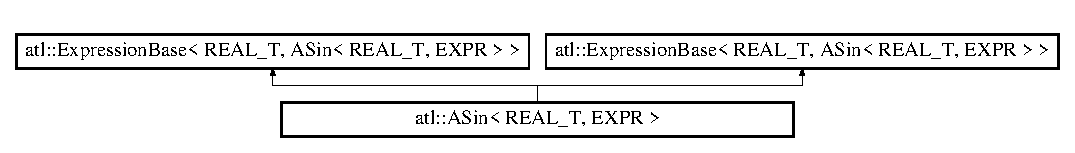
\includegraphics[height=1.613833cm]{structatl_1_1_a_sin}
\end{center}
\end{figure}
\subsection*{Public Types}
\begin{DoxyCompactItemize}
\item 
\hypertarget{structatl_1_1_a_sin_a85da08527224ed087dff8ac44e1ad203}{typedef R\+E\+A\+L\+\_\+\+T {\bfseries B\+A\+S\+E\+\_\+\+T\+Y\+P\+E}}\label{structatl_1_1_a_sin_a85da08527224ed087dff8ac44e1ad203}

\item 
\hypertarget{structatl_1_1_a_sin_a85da08527224ed087dff8ac44e1ad203}{typedef R\+E\+A\+L\+\_\+\+T {\bfseries B\+A\+S\+E\+\_\+\+T\+Y\+P\+E}}\label{structatl_1_1_a_sin_a85da08527224ed087dff8ac44e1ad203}

\end{DoxyCompactItemize}
\subsection*{Public Member Functions}
\begin{DoxyCompactItemize}
\item 
\hyperlink{structatl_1_1_a_sin_a78dd6e912643cfb931c91b0cdcd86775}{A\+Sin} (const \hyperlink{structatl_1_1_expression_base}{Expression\+Base}$<$ R\+E\+A\+L\+\_\+\+T, E\+X\+P\+R $>$ \&a)
\item 
const R\+E\+A\+L\+\_\+\+T \hyperlink{structatl_1_1_a_sin_a735c2c1455ac56357b45891d6e1e89e9}{Get\+Value} () const 
\item 
const R\+E\+A\+L\+\_\+\+T \hyperlink{structatl_1_1_a_sin_a3495a8c2cfae3128fb661f70d4a81f66}{Get\+Value} (size\+\_\+t i, size\+\_\+t j=0) const 
\item 
bool \hyperlink{structatl_1_1_a_sin_aed481e77dce3a87099dcdabbba02ec9c}{Is\+Nonlinear} () const 
\item 
void \hyperlink{structatl_1_1_a_sin_a9ce7699eb3a349c5aef84ae5b300571e}{Push\+Ids} (typename \hyperlink{structatl_1_1_stack_entry}{atl\+::\+Stack\+Entry}$<$ R\+E\+A\+L\+\_\+\+T $>$\+::vi\+\_\+storage \&ids) const 
\item 
void \hyperlink{structatl_1_1_a_sin_a87876d1ff74017c2db8fb4f83dc6f812}{Push\+Ids} (typename \hyperlink{structatl_1_1_stack_entry}{atl\+::\+Stack\+Entry}$<$ R\+E\+A\+L\+\_\+\+T $>$\+::vi\+\_\+storage \&ids, size\+\_\+t i, size\+\_\+t j=0) const 
\item 
const R\+E\+A\+L\+\_\+\+T \hyperlink{structatl_1_1_a_sin_a280bb07b162a39a6007bd2babd7b068c}{Evaluate\+Derivative} (uint32\+\_\+t x) const 
\item 
R\+E\+A\+L\+\_\+\+T \hyperlink{structatl_1_1_a_sin_ac66a19f09203233fcbce5940d7b3ea09}{Evaluate\+Derivative} (uint32\+\_\+t x, uint32\+\_\+t y) const 
\item 
R\+E\+A\+L\+\_\+\+T \hyperlink{structatl_1_1_a_sin_a2515923288ec66684e1590efcaaa34e6}{Evaluate\+Derivative} (uint32\+\_\+t x, uint32\+\_\+t y, uint32\+\_\+t z) const 
\item 
const R\+E\+A\+L\+\_\+\+T \hyperlink{structatl_1_1_a_sin_accb124b6b3142902322b2c1c35ead579}{Evaluate\+Derivative} (uint32\+\_\+t x, size\+\_\+t i, size\+\_\+t j=0) const 
\item 
R\+E\+A\+L\+\_\+\+T \hyperlink{structatl_1_1_a_sin_a4e0b56394333abdb3b9f227cf22f56cf}{Evaluate\+Derivative} (uint32\+\_\+t x, uint32\+\_\+t y, size\+\_\+t i, size\+\_\+t j=0) const 
\item 
R\+E\+A\+L\+\_\+\+T \hyperlink{structatl_1_1_a_sin_ae6ef55e7cb8cad6613c278d4acd9e9a5}{Evaluate\+Derivative} (uint32\+\_\+t x, uint32\+\_\+t y, uint32\+\_\+t z, size\+\_\+t i, size\+\_\+t j=0) const 
\item 
size\+\_\+t \hyperlink{structatl_1_1_a_sin_ac543bb3714f66197d82872d95597c4fa}{Get\+Columns} () const 
\item 
size\+\_\+t \hyperlink{structatl_1_1_a_sin_ad81c947c1c246f0b8632c4a76b6abd25}{Get\+Rows} () const 
\item 
bool \hyperlink{structatl_1_1_a_sin_a08317f212ec6e8ee67dff39c5a50dc65}{Is\+Scalar} () const 
\item 
const std\+::string \hyperlink{structatl_1_1_a_sin_a9aead25825a033a090f9f6251d87ba12}{To\+Expression\+Template\+String} () const 
\item 
\hypertarget{structatl_1_1_a_sin_a78dd6e912643cfb931c91b0cdcd86775}{{\bfseries A\+Sin} (const \hyperlink{structatl_1_1_expression_base}{Expression\+Base}$<$ R\+E\+A\+L\+\_\+\+T, E\+X\+P\+R $>$ \&a)}\label{structatl_1_1_a_sin_a78dd6e912643cfb931c91b0cdcd86775}

\item 
\hypertarget{structatl_1_1_a_sin_a735c2c1455ac56357b45891d6e1e89e9}{const R\+E\+A\+L\+\_\+\+T {\bfseries Get\+Value} () const }\label{structatl_1_1_a_sin_a735c2c1455ac56357b45891d6e1e89e9}

\item 
\hypertarget{structatl_1_1_a_sin_a3495a8c2cfae3128fb661f70d4a81f66}{const R\+E\+A\+L\+\_\+\+T {\bfseries Get\+Value} (size\+\_\+t i, size\+\_\+t j=0) const }\label{structatl_1_1_a_sin_a3495a8c2cfae3128fb661f70d4a81f66}

\item 
\hypertarget{structatl_1_1_a_sin_a9ce7699eb3a349c5aef84ae5b300571e}{void {\bfseries Push\+Ids} (typename \hyperlink{structatl_1_1_stack_entry}{atl\+::\+Stack\+Entry}$<$ R\+E\+A\+L\+\_\+\+T $>$\+::vi\+\_\+storage \&ids) const }\label{structatl_1_1_a_sin_a9ce7699eb3a349c5aef84ae5b300571e}

\item 
\hypertarget{structatl_1_1_a_sin_a87876d1ff74017c2db8fb4f83dc6f812}{void {\bfseries Push\+Ids} (typename \hyperlink{structatl_1_1_stack_entry}{atl\+::\+Stack\+Entry}$<$ R\+E\+A\+L\+\_\+\+T $>$\+::vi\+\_\+storage \&ids, size\+\_\+t i, size\+\_\+t j=0) const }\label{structatl_1_1_a_sin_a87876d1ff74017c2db8fb4f83dc6f812}

\item 
\hypertarget{structatl_1_1_a_sin_af850f9d56fe01515d9d3160634ea0b97}{const R\+E\+A\+L\+\_\+\+T {\bfseries Evaluate\+Derivative} (uint32\+\_\+t id) const }\label{structatl_1_1_a_sin_af850f9d56fe01515d9d3160634ea0b97}

\item 
\hypertarget{structatl_1_1_a_sin_aa5264797e90b72409c5025edf26d8465}{R\+E\+A\+L\+\_\+\+T {\bfseries Evaluate\+Derivative} (uint32\+\_\+t a, uint32\+\_\+t b) const }\label{structatl_1_1_a_sin_aa5264797e90b72409c5025edf26d8465}

\item 
\hypertarget{structatl_1_1_a_sin_a2515923288ec66684e1590efcaaa34e6}{R\+E\+A\+L\+\_\+\+T {\bfseries Evaluate\+Derivative} (uint32\+\_\+t x, uint32\+\_\+t y, uint32\+\_\+t z) const }\label{structatl_1_1_a_sin_a2515923288ec66684e1590efcaaa34e6}

\item 
\hypertarget{structatl_1_1_a_sin_a55e723783221a14bc4e92bfc7d1d2a97}{const R\+E\+A\+L\+\_\+\+T {\bfseries Evaluate\+Derivative} (uint32\+\_\+t id, size\+\_\+t i, size\+\_\+t j=0) const }\label{structatl_1_1_a_sin_a55e723783221a14bc4e92bfc7d1d2a97}

\item 
\hypertarget{structatl_1_1_a_sin_a49dd7c592a71b1d2e813c91864475d9f}{R\+E\+A\+L\+\_\+\+T {\bfseries Evaluate\+Derivative} (uint32\+\_\+t a, uint32\+\_\+t b, size\+\_\+t i, size\+\_\+t j=0) const }\label{structatl_1_1_a_sin_a49dd7c592a71b1d2e813c91864475d9f}

\item 
\hypertarget{structatl_1_1_a_sin_ae6ef55e7cb8cad6613c278d4acd9e9a5}{R\+E\+A\+L\+\_\+\+T {\bfseries Evaluate\+Derivative} (uint32\+\_\+t x, uint32\+\_\+t y, uint32\+\_\+t z, size\+\_\+t i, size\+\_\+t j=0) const }\label{structatl_1_1_a_sin_ae6ef55e7cb8cad6613c278d4acd9e9a5}

\item 
\hypertarget{structatl_1_1_a_sin_ac543bb3714f66197d82872d95597c4fa}{size\+\_\+t {\bfseries Get\+Columns} () const }\label{structatl_1_1_a_sin_ac543bb3714f66197d82872d95597c4fa}

\item 
\hypertarget{structatl_1_1_a_sin_ad81c947c1c246f0b8632c4a76b6abd25}{size\+\_\+t {\bfseries Get\+Rows} () const }\label{structatl_1_1_a_sin_ad81c947c1c246f0b8632c4a76b6abd25}

\item 
\hypertarget{structatl_1_1_a_sin_a08317f212ec6e8ee67dff39c5a50dc65}{bool {\bfseries Is\+Scalar} () const }\label{structatl_1_1_a_sin_a08317f212ec6e8ee67dff39c5a50dc65}

\end{DoxyCompactItemize}
\subsection*{Public Attributes}
\begin{DoxyCompactItemize}
\item 
\hypertarget{structatl_1_1_a_sin_a76130f5a52cb5453fd0308d48413b0e1}{const E\+X\+P\+R \& {\bfseries expr\+\_\+m}}\label{structatl_1_1_a_sin_a76130f5a52cb5453fd0308d48413b0e1}

\end{DoxyCompactItemize}


\subsection{Detailed Description}
\subsubsection*{template$<$class R\+E\+A\+L\+\_\+\+T, class E\+X\+P\+R$>$struct atl\+::\+A\+Sin$<$ R\+E\+A\+L\+\_\+\+T, E\+X\+P\+R $>$}

Expression template to handle arcsine for variable or container expressions.

$ \arcsin f(x,y) $

or

$ \arcsin f_{i,j}(x,y) $ 

\subsection{Constructor \& Destructor Documentation}
\hypertarget{structatl_1_1_a_sin_a78dd6e912643cfb931c91b0cdcd86775}{\index{atl\+::\+A\+Sin@{atl\+::\+A\+Sin}!A\+Sin@{A\+Sin}}
\index{A\+Sin@{A\+Sin}!atl\+::\+A\+Sin@{atl\+::\+A\+Sin}}
\subsubsection[{A\+Sin}]{\setlength{\rightskip}{0pt plus 5cm}template$<$class R\+E\+A\+L\+\_\+\+T , class E\+X\+P\+R $>$ {\bf atl\+::\+A\+Sin}$<$ R\+E\+A\+L\+\_\+\+T, E\+X\+P\+R $>$\+::{\bf A\+Sin} (
\begin{DoxyParamCaption}
\item[{const {\bf Expression\+Base}$<$ R\+E\+A\+L\+\_\+\+T, E\+X\+P\+R $>$ \&}]{a}
\end{DoxyParamCaption}
)\hspace{0.3cm}{\ttfamily [inline]}}}\label{structatl_1_1_a_sin_a78dd6e912643cfb931c91b0cdcd86775}
Constructor


\begin{DoxyParams}{Parameters}
{\em a} & \\
\hline
\end{DoxyParams}


\subsection{Member Function Documentation}
\hypertarget{structatl_1_1_a_sin_a280bb07b162a39a6007bd2babd7b068c}{\index{atl\+::\+A\+Sin@{atl\+::\+A\+Sin}!Evaluate\+Derivative@{Evaluate\+Derivative}}
\index{Evaluate\+Derivative@{Evaluate\+Derivative}!atl\+::\+A\+Sin@{atl\+::\+A\+Sin}}
\subsubsection[{Evaluate\+Derivative}]{\setlength{\rightskip}{0pt plus 5cm}template$<$class R\+E\+A\+L\+\_\+\+T , class E\+X\+P\+R $>$ const R\+E\+A\+L\+\_\+\+T {\bf atl\+::\+A\+Sin}$<$ R\+E\+A\+L\+\_\+\+T, E\+X\+P\+R $>$\+::Evaluate\+Derivative (
\begin{DoxyParamCaption}
\item[{uint32\+\_\+t}]{x}
\end{DoxyParamCaption}
) const\hspace{0.3cm}{\ttfamily [inline]}}}\label{structatl_1_1_a_sin_a280bb07b162a39a6007bd2babd7b068c}
Evaluates the first-\/order derivative of this expression with respect to x.

$ {{{{d}\over{d\,x}}\,f\left(x\right)}\over{\sqrt{1-f^2\left(x\right)}}} $ 
\begin{DoxyParams}{Parameters}
{\em x} & \\
\hline
\end{DoxyParams}
\begin{DoxyReturn}{Returns}

\end{DoxyReturn}
\hypertarget{structatl_1_1_a_sin_ac66a19f09203233fcbce5940d7b3ea09}{\index{atl\+::\+A\+Sin@{atl\+::\+A\+Sin}!Evaluate\+Derivative@{Evaluate\+Derivative}}
\index{Evaluate\+Derivative@{Evaluate\+Derivative}!atl\+::\+A\+Sin@{atl\+::\+A\+Sin}}
\subsubsection[{Evaluate\+Derivative}]{\setlength{\rightskip}{0pt plus 5cm}template$<$class R\+E\+A\+L\+\_\+\+T , class E\+X\+P\+R $>$ R\+E\+A\+L\+\_\+\+T {\bf atl\+::\+A\+Sin}$<$ R\+E\+A\+L\+\_\+\+T, E\+X\+P\+R $>$\+::Evaluate\+Derivative (
\begin{DoxyParamCaption}
\item[{uint32\+\_\+t}]{x, }
\item[{uint32\+\_\+t}]{y}
\end{DoxyParamCaption}
) const\hspace{0.3cm}{\ttfamily [inline]}}}\label{structatl_1_1_a_sin_ac66a19f09203233fcbce5940d7b3ea09}
Evaluates the second-\/order mixed partial with respect to x and y.

$ {{f(x,y)\,\left({{d}\over{d\,x}}\,f(x,y)\right)\,\left( {{d}\over{d\,y}}\,f(x,y)\right)}\over{\left(1-f(x,y)^2 \right)^{{{3}\over{2}}}}}+{{{{d^2}\over{d\,x\,d\,y}}\,f(x,y) }\over{\sqrt{1-f(x,y)^2}}} $


\begin{DoxyParams}{Parameters}
{\em x} & \\
\hline
{\em y} & \\
\hline
{\em i} & \\
\hline
{\em j} & \\
\hline
\end{DoxyParams}
\begin{DoxyReturn}{Returns}

\end{DoxyReturn}
\hypertarget{structatl_1_1_a_sin_a2515923288ec66684e1590efcaaa34e6}{\index{atl\+::\+A\+Sin@{atl\+::\+A\+Sin}!Evaluate\+Derivative@{Evaluate\+Derivative}}
\index{Evaluate\+Derivative@{Evaluate\+Derivative}!atl\+::\+A\+Sin@{atl\+::\+A\+Sin}}
\subsubsection[{Evaluate\+Derivative}]{\setlength{\rightskip}{0pt plus 5cm}template$<$class R\+E\+A\+L\+\_\+\+T , class E\+X\+P\+R $>$ R\+E\+A\+L\+\_\+\+T {\bf atl\+::\+A\+Sin}$<$ R\+E\+A\+L\+\_\+\+T, E\+X\+P\+R $>$\+::Evaluate\+Derivative (
\begin{DoxyParamCaption}
\item[{uint32\+\_\+t}]{x, }
\item[{uint32\+\_\+t}]{y, }
\item[{uint32\+\_\+t}]{z}
\end{DoxyParamCaption}
) const\hspace{0.3cm}{\ttfamily [inline]}}}\label{structatl_1_1_a_sin_a2515923288ec66684e1590efcaaa34e6}
Evaluates the third-\/order mixed partial with respect to x,y, and z.

$ {{{{d}\over{d\,x}}\,f\left(x , y , z\right)\,\left({{d}\over{d\,y}} \,f\left(x , y , z\right)\right)\,\left({{d}\over{d\,z}}\,f\left(x , y , z\right)\right)}\over{\left(1-f^2\left(x , y , z\right) \right)^{{{3}\over{2}}}}}+{{3\,f^2\left(x , y , z\right)\,\left({{d }\over{d\,x}}\,f\left(x , y , z\right)\right)\,\left({{d}\over{d\,y }}\,f\left(x , y , z\right)\right)\,\left({{d}\over{d\,z}}\,f\left(x , y , z\right)\right)}\over{\left(1-f^2\left(x , y , z\right) \right)^{{{5}\over{2}}}}}+{{f\left(x , y , z\right)\,\left({{d^2 }\over{d\,x\,d\,y}}\,f\left(x , y , z\right)\right)\,\left({{d }\over{d\,z}}\,f\left(x , y , z\right)\right)}\over{\left(1-f^2 \left(x , y , z\right)\right)^{{{3}\over{2}}}}}+ \\ {{f\left(x , y , z \right)\,\left({{d}\over{d\,x}}\,f\left(x , y , z\right)\right)\, \left({{d^2}\over{d\,y\,d\,z}}\,f\left(x , y , z\right)\right) }\over{\left(1-f^2\left(x , y , z\right)\right)^{{{3}\over{2}}}}}+{{ f\left(x , y , z\right)\,\left({{d^2}\over{d\,x\,d\,z}}\,f\left(x , y , z\right)\right)\,\left({{d}\over{d\,y}}\,f\left(x , y , z\right) \right)}\over{\left(1-f^2\left(x , y , z\right)\right)^{{{3}\over{2 }}}}}+{{{{d^3}\over{d\,x\,d\,y\,d\,z}}\,f\left(x , y , z\right) }\over{\sqrt{1-f^2\left(x , y , z\right)}}} $


\begin{DoxyParams}{Parameters}
{\em x} & \\
\hline
{\em y} & \\
\hline
{\em z} & \\
\hline
\end{DoxyParams}
\begin{DoxyReturn}{Returns}

\end{DoxyReturn}
\hypertarget{structatl_1_1_a_sin_accb124b6b3142902322b2c1c35ead579}{\index{atl\+::\+A\+Sin@{atl\+::\+A\+Sin}!Evaluate\+Derivative@{Evaluate\+Derivative}}
\index{Evaluate\+Derivative@{Evaluate\+Derivative}!atl\+::\+A\+Sin@{atl\+::\+A\+Sin}}
\subsubsection[{Evaluate\+Derivative}]{\setlength{\rightskip}{0pt plus 5cm}template$<$class R\+E\+A\+L\+\_\+\+T , class E\+X\+P\+R $>$ const R\+E\+A\+L\+\_\+\+T {\bf atl\+::\+A\+Sin}$<$ R\+E\+A\+L\+\_\+\+T, E\+X\+P\+R $>$\+::Evaluate\+Derivative (
\begin{DoxyParamCaption}
\item[{uint32\+\_\+t}]{x, }
\item[{size\+\_\+t}]{i, }
\item[{size\+\_\+t}]{j = {\ttfamily 0}}
\end{DoxyParamCaption}
) const\hspace{0.3cm}{\ttfamily [inline]}}}\label{structatl_1_1_a_sin_accb124b6b3142902322b2c1c35ead579}
Evaluates the first-\/order derivative of this expression with respect to x.

$ {{{{d}\over{d\,x}}\,f_{i,j}(x)}\over{\sqrt{1-f_{i,j}(x)^2}}} $


\begin{DoxyParams}{Parameters}
{\em x} & \\
\hline
{\em i} & \\
\hline
{\em j} & \\
\hline
\end{DoxyParams}
\begin{DoxyReturn}{Returns}

\end{DoxyReturn}
\hypertarget{structatl_1_1_a_sin_a4e0b56394333abdb3b9f227cf22f56cf}{\index{atl\+::\+A\+Sin@{atl\+::\+A\+Sin}!Evaluate\+Derivative@{Evaluate\+Derivative}}
\index{Evaluate\+Derivative@{Evaluate\+Derivative}!atl\+::\+A\+Sin@{atl\+::\+A\+Sin}}
\subsubsection[{Evaluate\+Derivative}]{\setlength{\rightskip}{0pt plus 5cm}template$<$class R\+E\+A\+L\+\_\+\+T , class E\+X\+P\+R $>$ R\+E\+A\+L\+\_\+\+T {\bf atl\+::\+A\+Sin}$<$ R\+E\+A\+L\+\_\+\+T, E\+X\+P\+R $>$\+::Evaluate\+Derivative (
\begin{DoxyParamCaption}
\item[{uint32\+\_\+t}]{x, }
\item[{uint32\+\_\+t}]{y, }
\item[{size\+\_\+t}]{i, }
\item[{size\+\_\+t}]{j = {\ttfamily 0}}
\end{DoxyParamCaption}
) const\hspace{0.3cm}{\ttfamily [inline]}}}\label{structatl_1_1_a_sin_a4e0b56394333abdb3b9f227cf22f56cf}
Evaluates the second-\/order mixed partial with respect to x and y at index \{i,j\}.

$ {{f_{i,j}(x,y)\,\left({{d}\over{d\,x}}\,f_{i,j}(x,y)\right)\,\left( {{d}\over{d\,y}}\,f_{i,j}(x,y)\right)}\over{\left(1-f_{i,j}(x,y)^2 \right)^{{{3}\over{2}}}}}+{{{{d^2}\over{d\,x\,d\,y}}\,f_{i,j}(x,y) }\over{\sqrt{1-f_{i,j}(x,y)^2}}} $


\begin{DoxyParams}{Parameters}
{\em x} & \\
\hline
{\em y} & \\
\hline
{\em i} & \\
\hline
{\em j} & \\
\hline
\end{DoxyParams}
\begin{DoxyReturn}{Returns}

\end{DoxyReturn}
\hypertarget{structatl_1_1_a_sin_ae6ef55e7cb8cad6613c278d4acd9e9a5}{\index{atl\+::\+A\+Sin@{atl\+::\+A\+Sin}!Evaluate\+Derivative@{Evaluate\+Derivative}}
\index{Evaluate\+Derivative@{Evaluate\+Derivative}!atl\+::\+A\+Sin@{atl\+::\+A\+Sin}}
\subsubsection[{Evaluate\+Derivative}]{\setlength{\rightskip}{0pt plus 5cm}template$<$class R\+E\+A\+L\+\_\+\+T , class E\+X\+P\+R $>$ R\+E\+A\+L\+\_\+\+T {\bf atl\+::\+A\+Sin}$<$ R\+E\+A\+L\+\_\+\+T, E\+X\+P\+R $>$\+::Evaluate\+Derivative (
\begin{DoxyParamCaption}
\item[{uint32\+\_\+t}]{x, }
\item[{uint32\+\_\+t}]{y, }
\item[{uint32\+\_\+t}]{z, }
\item[{size\+\_\+t}]{i, }
\item[{size\+\_\+t}]{j = {\ttfamily 0}}
\end{DoxyParamCaption}
) const\hspace{0.3cm}{\ttfamily [inline]}}}\label{structatl_1_1_a_sin_ae6ef55e7cb8cad6613c278d4acd9e9a5}
Evaluates the third-\/order mixed partial with respect to x,y, and z at index \{i,j\}.

$ {{{{d}\over{d\,x}}\,f_{i,j}(x,y,z)\,\left({{d}\over{d\,y}}\,f_{i,j} (x,y,z)\right)\,\left({{d}\over{d\,z}}\,f_{i,j}(x,y,z)\right)}\over{ \left(1-f_{i,j}(x,y,z)^2\right)^{{{3}\over{2}}}}}+{{3\,f_{i,j}(x,y,z )^2\,\left({{d}\over{d\,x}}\,f_{i,j}(x,y,z)\right)\,\left({{d}\over{ d\,y}}\,f_{i,j}(x,y,z)\right)\,\left({{d}\over{d\,z}}\,f_{i,j}(x,y,z )\right)}\over{\left(1-f_{i,j}(x,y,z)^2\right)^{{{5}\over{2}}}}}+{{f _{i,j}(x,y,z)\,\left({{d^2}\over{d\,x\,d\,y}}\,f_{i,j}(x,y,z)\right) \,\left({{d}\over{d\,z}}\,f_{i,j}(x,y,z)\right)}\over{\left(1-f_{i,j }(x,y,z)^2\right)^{{{3}\over{2}}}}}+ \\ {{f_{i,j}(x,y,z)\,\left({{d }\over{d\,x}}\,f_{i,j}(x,y,z)\right)\,\left({{d^2}\over{d\,y\,d\,z}} \,f_{i,j}(x,y,z)\right)}\over{\left(1-f_{i,j}(x,y,z)^2\right)^{{{3 }\over{2}}}}}+{{f_{i,j}(x,y,z)\,\left({{d^2}\over{d\,x\,d\,z}}\,f_{i ,j}(x,y,z)\right)\,\left({{d}\over{d\,y}}\,f_{i,j}(x,y,z)\right) }\over{\left(1-f_{i,j}(x,y,z)^2\right)^{{{3}\over{2}}}}}+{{{{d^3 }\over{d\,x\,d\,y\,d\,z}}\,f_{i,j}(x,y,z)}\over{\sqrt{1-f_{i,j}(x,y, z)^2}}} $


\begin{DoxyParams}{Parameters}
{\em x} & \\
\hline
{\em y} & \\
\hline
{\em z} & \\
\hline
{\em i} & \\
\hline
{\em j} & \\
\hline
\end{DoxyParams}
\begin{DoxyReturn}{Returns}

\end{DoxyReturn}
\hypertarget{structatl_1_1_a_sin_ac543bb3714f66197d82872d95597c4fa}{\index{atl\+::\+A\+Sin@{atl\+::\+A\+Sin}!Get\+Columns@{Get\+Columns}}
\index{Get\+Columns@{Get\+Columns}!atl\+::\+A\+Sin@{atl\+::\+A\+Sin}}
\subsubsection[{Get\+Columns}]{\setlength{\rightskip}{0pt plus 5cm}template$<$class R\+E\+A\+L\+\_\+\+T , class E\+X\+P\+R $>$ size\+\_\+t {\bf atl\+::\+A\+Sin}$<$ R\+E\+A\+L\+\_\+\+T, E\+X\+P\+R $>$\+::Get\+Columns (
\begin{DoxyParamCaption}
{}
\end{DoxyParamCaption}
) const\hspace{0.3cm}{\ttfamily [inline]}}}\label{structatl_1_1_a_sin_ac543bb3714f66197d82872d95597c4fa}
Return the number of columns.

\begin{DoxyReturn}{Returns}

\end{DoxyReturn}
\hypertarget{structatl_1_1_a_sin_ad81c947c1c246f0b8632c4a76b6abd25}{\index{atl\+::\+A\+Sin@{atl\+::\+A\+Sin}!Get\+Rows@{Get\+Rows}}
\index{Get\+Rows@{Get\+Rows}!atl\+::\+A\+Sin@{atl\+::\+A\+Sin}}
\subsubsection[{Get\+Rows}]{\setlength{\rightskip}{0pt plus 5cm}template$<$class R\+E\+A\+L\+\_\+\+T , class E\+X\+P\+R $>$ size\+\_\+t {\bf atl\+::\+A\+Sin}$<$ R\+E\+A\+L\+\_\+\+T, E\+X\+P\+R $>$\+::Get\+Rows (
\begin{DoxyParamCaption}
{}
\end{DoxyParamCaption}
) const\hspace{0.3cm}{\ttfamily [inline]}}}\label{structatl_1_1_a_sin_ad81c947c1c246f0b8632c4a76b6abd25}
Return the number of rows.

\begin{DoxyReturn}{Returns}

\end{DoxyReturn}
\hypertarget{structatl_1_1_a_sin_a735c2c1455ac56357b45891d6e1e89e9}{\index{atl\+::\+A\+Sin@{atl\+::\+A\+Sin}!Get\+Value@{Get\+Value}}
\index{Get\+Value@{Get\+Value}!atl\+::\+A\+Sin@{atl\+::\+A\+Sin}}
\subsubsection[{Get\+Value}]{\setlength{\rightskip}{0pt plus 5cm}template$<$class R\+E\+A\+L\+\_\+\+T , class E\+X\+P\+R $>$ const R\+E\+A\+L\+\_\+\+T {\bf atl\+::\+A\+Sin}$<$ R\+E\+A\+L\+\_\+\+T, E\+X\+P\+R $>$\+::Get\+Value (
\begin{DoxyParamCaption}
{}
\end{DoxyParamCaption}
) const\hspace{0.3cm}{\ttfamily [inline]}}}\label{structatl_1_1_a_sin_a735c2c1455ac56357b45891d6e1e89e9}
Compute the arcsine of the expression evaluated.

\begin{DoxyReturn}{Returns}

\end{DoxyReturn}
\hypertarget{structatl_1_1_a_sin_a3495a8c2cfae3128fb661f70d4a81f66}{\index{atl\+::\+A\+Sin@{atl\+::\+A\+Sin}!Get\+Value@{Get\+Value}}
\index{Get\+Value@{Get\+Value}!atl\+::\+A\+Sin@{atl\+::\+A\+Sin}}
\subsubsection[{Get\+Value}]{\setlength{\rightskip}{0pt plus 5cm}template$<$class R\+E\+A\+L\+\_\+\+T , class E\+X\+P\+R $>$ const R\+E\+A\+L\+\_\+\+T {\bf atl\+::\+A\+Sin}$<$ R\+E\+A\+L\+\_\+\+T, E\+X\+P\+R $>$\+::Get\+Value (
\begin{DoxyParamCaption}
\item[{size\+\_\+t}]{i, }
\item[{size\+\_\+t}]{j = {\ttfamily 0}}
\end{DoxyParamCaption}
) const\hspace{0.3cm}{\ttfamily [inline]}}}\label{structatl_1_1_a_sin_a3495a8c2cfae3128fb661f70d4a81f66}
Compute the arcsine of the expression evaluated at index \{i,j\}.

\begin{DoxyReturn}{Returns}

\end{DoxyReturn}
\hypertarget{structatl_1_1_a_sin_aed481e77dce3a87099dcdabbba02ec9c}{\index{atl\+::\+A\+Sin@{atl\+::\+A\+Sin}!Is\+Nonlinear@{Is\+Nonlinear}}
\index{Is\+Nonlinear@{Is\+Nonlinear}!atl\+::\+A\+Sin@{atl\+::\+A\+Sin}}
\subsubsection[{Is\+Nonlinear}]{\setlength{\rightskip}{0pt plus 5cm}template$<$class R\+E\+A\+L\+\_\+\+T , class E\+X\+P\+R $>$ bool {\bf atl\+::\+A\+Sin}$<$ R\+E\+A\+L\+\_\+\+T, E\+X\+P\+R $>$\+::Is\+Nonlinear (
\begin{DoxyParamCaption}
{}
\end{DoxyParamCaption}
) const\hspace{0.3cm}{\ttfamily [inline]}}}\label{structatl_1_1_a_sin_aed481e77dce3a87099dcdabbba02ec9c}
Returns true.

\begin{DoxyReturn}{Returns}

\end{DoxyReturn}
\hypertarget{structatl_1_1_a_sin_a08317f212ec6e8ee67dff39c5a50dc65}{\index{atl\+::\+A\+Sin@{atl\+::\+A\+Sin}!Is\+Scalar@{Is\+Scalar}}
\index{Is\+Scalar@{Is\+Scalar}!atl\+::\+A\+Sin@{atl\+::\+A\+Sin}}
\subsubsection[{Is\+Scalar}]{\setlength{\rightskip}{0pt plus 5cm}template$<$class R\+E\+A\+L\+\_\+\+T , class E\+X\+P\+R $>$ bool {\bf atl\+::\+A\+Sin}$<$ R\+E\+A\+L\+\_\+\+T, E\+X\+P\+R $>$\+::Is\+Scalar (
\begin{DoxyParamCaption}
{}
\end{DoxyParamCaption}
) const\hspace{0.3cm}{\ttfamily [inline]}}}\label{structatl_1_1_a_sin_a08317f212ec6e8ee67dff39c5a50dc65}
True if this expression is a scalar.

\begin{DoxyReturn}{Returns}

\end{DoxyReturn}
\hypertarget{structatl_1_1_a_sin_a9ce7699eb3a349c5aef84ae5b300571e}{\index{atl\+::\+A\+Sin@{atl\+::\+A\+Sin}!Push\+Ids@{Push\+Ids}}
\index{Push\+Ids@{Push\+Ids}!atl\+::\+A\+Sin@{atl\+::\+A\+Sin}}
\subsubsection[{Push\+Ids}]{\setlength{\rightskip}{0pt plus 5cm}template$<$class R\+E\+A\+L\+\_\+\+T , class E\+X\+P\+R $>$ void {\bf atl\+::\+A\+Sin}$<$ R\+E\+A\+L\+\_\+\+T, E\+X\+P\+R $>$\+::Push\+Ids (
\begin{DoxyParamCaption}
\item[{typename {\bf atl\+::\+Stack\+Entry}$<$ R\+E\+A\+L\+\_\+\+T $>$\+::vi\+\_\+storage \&}]{ids}
\end{DoxyParamCaption}
) const\hspace{0.3cm}{\ttfamily [inline]}}}\label{structatl_1_1_a_sin_a9ce7699eb3a349c5aef84ae5b300571e}
Push variable info into a set.


\begin{DoxyParams}{Parameters}
{\em ids} & \\
\hline
{\em i} & \\
\hline
{\em j} & \\
\hline
\end{DoxyParams}
\hypertarget{structatl_1_1_a_sin_a87876d1ff74017c2db8fb4f83dc6f812}{\index{atl\+::\+A\+Sin@{atl\+::\+A\+Sin}!Push\+Ids@{Push\+Ids}}
\index{Push\+Ids@{Push\+Ids}!atl\+::\+A\+Sin@{atl\+::\+A\+Sin}}
\subsubsection[{Push\+Ids}]{\setlength{\rightskip}{0pt plus 5cm}template$<$class R\+E\+A\+L\+\_\+\+T , class E\+X\+P\+R $>$ void {\bf atl\+::\+A\+Sin}$<$ R\+E\+A\+L\+\_\+\+T, E\+X\+P\+R $>$\+::Push\+Ids (
\begin{DoxyParamCaption}
\item[{typename {\bf atl\+::\+Stack\+Entry}$<$ R\+E\+A\+L\+\_\+\+T $>$\+::vi\+\_\+storage \&}]{ids, }
\item[{size\+\_\+t}]{i, }
\item[{size\+\_\+t}]{j = {\ttfamily 0}}
\end{DoxyParamCaption}
) const\hspace{0.3cm}{\ttfamily [inline]}}}\label{structatl_1_1_a_sin_a87876d1ff74017c2db8fb4f83dc6f812}
Push variable info into a set at index \{i,j\}.


\begin{DoxyParams}{Parameters}
{\em ids} & \\
\hline
{\em i} & \\
\hline
{\em j} & \\
\hline
\end{DoxyParams}
\hypertarget{structatl_1_1_a_sin_a9aead25825a033a090f9f6251d87ba12}{\index{atl\+::\+A\+Sin@{atl\+::\+A\+Sin}!To\+Expression\+Template\+String@{To\+Expression\+Template\+String}}
\index{To\+Expression\+Template\+String@{To\+Expression\+Template\+String}!atl\+::\+A\+Sin@{atl\+::\+A\+Sin}}
\subsubsection[{To\+Expression\+Template\+String}]{\setlength{\rightskip}{0pt plus 5cm}template$<$class R\+E\+A\+L\+\_\+\+T , class E\+X\+P\+R $>$ const std\+::string {\bf atl\+::\+A\+Sin}$<$ R\+E\+A\+L\+\_\+\+T, E\+X\+P\+R $>$\+::To\+Expression\+Template\+String (
\begin{DoxyParamCaption}
{}
\end{DoxyParamCaption}
) const\hspace{0.3cm}{\ttfamily [inline]}}}\label{structatl_1_1_a_sin_a9aead25825a033a090f9f6251d87ba12}
Create a string representation of this expression template. \begin{DoxyReturn}{Returns}

\end{DoxyReturn}


The documentation for this struct was generated from the following file\+:\begin{DoxyCompactItemize}
\item 
A\+Sin.\+hpp\end{DoxyCompactItemize}

\hypertarget{structatl_1_1_a_tan}{\section{atl\+:\+:A\+Tan$<$ R\+E\+A\+L\+\_\+\+T, E\+X\+P\+R $>$ Struct Template Reference}
\label{structatl_1_1_a_tan}\index{atl\+::\+A\+Tan$<$ R\+E\+A\+L\+\_\+\+T, E\+X\+P\+R $>$@{atl\+::\+A\+Tan$<$ R\+E\+A\+L\+\_\+\+T, E\+X\+P\+R $>$}}
}


{\ttfamily \#include $<$A\+Tan.\+hpp$>$}

Inheritance diagram for atl\+:\+:A\+Tan$<$ R\+E\+A\+L\+\_\+\+T, E\+X\+P\+R $>$\+:\begin{figure}[H]
\begin{center}
\leavevmode
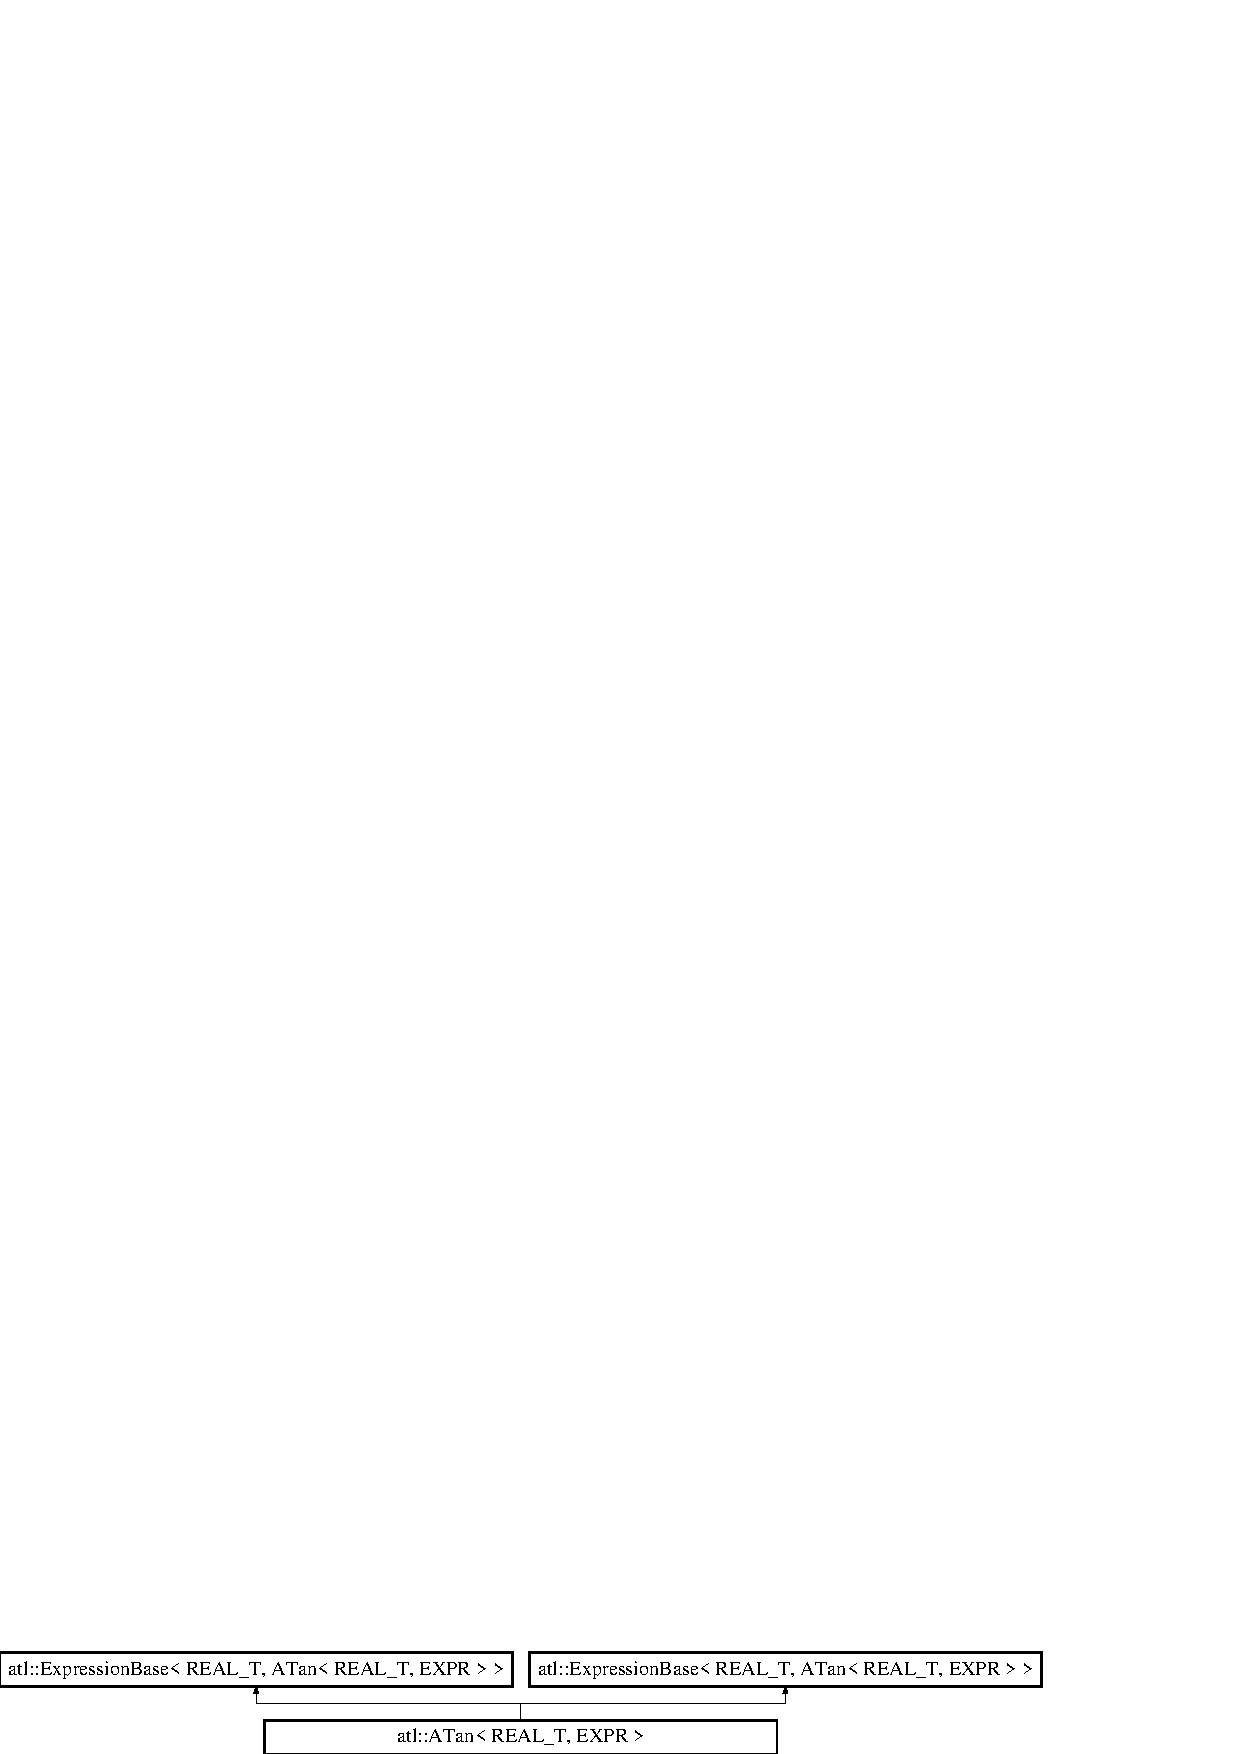
\includegraphics[height=1.600000cm]{structatl_1_1_a_tan}
\end{center}
\end{figure}
\subsection*{Public Types}
\begin{DoxyCompactItemize}
\item 
\hypertarget{structatl_1_1_a_tan_a28cc9b6f430e8999562bfa823a902914}{typedef R\+E\+A\+L\+\_\+\+T {\bfseries B\+A\+S\+E\+\_\+\+T\+Y\+P\+E}}\label{structatl_1_1_a_tan_a28cc9b6f430e8999562bfa823a902914}

\item 
\hypertarget{structatl_1_1_a_tan_a28cc9b6f430e8999562bfa823a902914}{typedef R\+E\+A\+L\+\_\+\+T {\bfseries B\+A\+S\+E\+\_\+\+T\+Y\+P\+E}}\label{structatl_1_1_a_tan_a28cc9b6f430e8999562bfa823a902914}

\end{DoxyCompactItemize}
\subsection*{Public Member Functions}
\begin{DoxyCompactItemize}
\item 
\hyperlink{structatl_1_1_a_tan_add096151fe20c8632a60c964878a4902}{A\+Tan} (const \hyperlink{structatl_1_1_expression_base}{Expression\+Base}$<$ R\+E\+A\+L\+\_\+\+T, E\+X\+P\+R $>$ \&a)
\item 
const R\+E\+A\+L\+\_\+\+T \hyperlink{structatl_1_1_a_tan_a0f02fc43a4a82a876e014d7fdaa1a0d9}{Get\+Value} () const 
\item 
const R\+E\+A\+L\+\_\+\+T \hyperlink{structatl_1_1_a_tan_a8eca69dbb72c27a6329e585e38390b47}{Get\+Value} (size\+\_\+t i, size\+\_\+t j=0) const 
\item 
bool \hyperlink{structatl_1_1_a_tan_a597d6ea253a631070cd06f4d2ad4a85e}{Is\+Nonlinear} () const 
\item 
void \hyperlink{structatl_1_1_a_tan_a687a1c79d9db4f2185eabfa553103a2d}{Push\+Ids} (typename \hyperlink{structatl_1_1_stack_entry}{atl\+::\+Stack\+Entry}$<$ R\+E\+A\+L\+\_\+\+T $>$\+::vi\+\_\+storage \&ids) const 
\item 
void \hyperlink{structatl_1_1_a_tan_ab5452739c72b6a25edba0ea6e0bb2a46}{Push\+Ids} (typename \hyperlink{structatl_1_1_stack_entry}{atl\+::\+Stack\+Entry}$<$ R\+E\+A\+L\+\_\+\+T $>$\+::vi\+\_\+storage \&ids, size\+\_\+t i, size\+\_\+t j=0) const 
\item 
const R\+E\+A\+L\+\_\+\+T \hyperlink{structatl_1_1_a_tan_a8abb6fe504290961d22d75e283406e9c}{Evaluate\+Derivative} (uint32\+\_\+t x) const 
\item 
R\+E\+A\+L\+\_\+\+T \hyperlink{structatl_1_1_a_tan_a6499ad9661bb99180537daab6c809ea4}{Evaluate\+Derivative} (uint32\+\_\+t x, uint32\+\_\+t y) const 
\item 
R\+E\+A\+L\+\_\+\+T \hyperlink{structatl_1_1_a_tan_a79de9c67b4b022ace970f951c53ba381}{Evaluate\+Derivative} (uint32\+\_\+t x, uint32\+\_\+t y, uint32\+\_\+t z) const 
\item 
const R\+E\+A\+L\+\_\+\+T \hyperlink{structatl_1_1_a_tan_a075d3de16cb0f1734c92784e8fd2089f}{Evaluate\+Derivative} (uint32\+\_\+t x, size\+\_\+t i, size\+\_\+t j=0) const 
\item 
R\+E\+A\+L\+\_\+\+T \hyperlink{structatl_1_1_a_tan_afaf84b97a4a37b7e4e8d6f9fbbcfc4ef}{Evaluate\+Derivative} (uint32\+\_\+t x, uint32\+\_\+t y, size\+\_\+t i, size\+\_\+t j=0) const 
\item 
R\+E\+A\+L\+\_\+\+T \hyperlink{structatl_1_1_a_tan_a48e1ff6400417eb0c724dba601bca61e}{Evaluate\+Derivative} (uint32\+\_\+t x, uint32\+\_\+t y, uint32\+\_\+t z, size\+\_\+t i, size\+\_\+t j=0) const 
\item 
size\+\_\+t \hyperlink{structatl_1_1_a_tan_a31a96dee4a7fb125fc32ab71be032c57}{Get\+Columns} () const 
\item 
size\+\_\+t \hyperlink{structatl_1_1_a_tan_a043abd1506434e38c581beb3da5182e8}{Get\+Rows} () const 
\item 
bool \hyperlink{structatl_1_1_a_tan_a0f3aa3f9327f314b64487f30a9ce0b75}{Is\+Scalar} () const 
\item 
const std\+::string \hyperlink{structatl_1_1_a_tan_a61c7cb4513cf240b4cff54350dfd4fe3}{To\+Expression\+Template\+String} () const 
\item 
\hypertarget{structatl_1_1_a_tan_add096151fe20c8632a60c964878a4902}{{\bfseries A\+Tan} (const \hyperlink{structatl_1_1_expression_base}{Expression\+Base}$<$ R\+E\+A\+L\+\_\+\+T, E\+X\+P\+R $>$ \&a)}\label{structatl_1_1_a_tan_add096151fe20c8632a60c964878a4902}

\item 
\hypertarget{structatl_1_1_a_tan_a0f02fc43a4a82a876e014d7fdaa1a0d9}{const R\+E\+A\+L\+\_\+\+T {\bfseries Get\+Value} () const }\label{structatl_1_1_a_tan_a0f02fc43a4a82a876e014d7fdaa1a0d9}

\item 
\hypertarget{structatl_1_1_a_tan_a8eca69dbb72c27a6329e585e38390b47}{const R\+E\+A\+L\+\_\+\+T {\bfseries Get\+Value} (size\+\_\+t i, size\+\_\+t j=0) const }\label{structatl_1_1_a_tan_a8eca69dbb72c27a6329e585e38390b47}

\item 
\hypertarget{structatl_1_1_a_tan_a687a1c79d9db4f2185eabfa553103a2d}{void {\bfseries Push\+Ids} (typename \hyperlink{structatl_1_1_stack_entry}{atl\+::\+Stack\+Entry}$<$ R\+E\+A\+L\+\_\+\+T $>$\+::vi\+\_\+storage \&ids) const }\label{structatl_1_1_a_tan_a687a1c79d9db4f2185eabfa553103a2d}

\item 
\hypertarget{structatl_1_1_a_tan_ab5452739c72b6a25edba0ea6e0bb2a46}{void {\bfseries Push\+Ids} (typename \hyperlink{structatl_1_1_stack_entry}{atl\+::\+Stack\+Entry}$<$ R\+E\+A\+L\+\_\+\+T $>$\+::vi\+\_\+storage \&ids, size\+\_\+t i, size\+\_\+t j=0) const }\label{structatl_1_1_a_tan_ab5452739c72b6a25edba0ea6e0bb2a46}

\item 
\hypertarget{structatl_1_1_a_tan_a8764410db8db30cd2aecf92114133649}{const R\+E\+A\+L\+\_\+\+T {\bfseries Evaluate\+Derivative} (uint32\+\_\+t id) const }\label{structatl_1_1_a_tan_a8764410db8db30cd2aecf92114133649}

\item 
\hypertarget{structatl_1_1_a_tan_ad1d203833ee881818c7fc95be026a88e}{R\+E\+A\+L\+\_\+\+T {\bfseries Evaluate\+Derivative} (uint32\+\_\+t a, uint32\+\_\+t b) const }\label{structatl_1_1_a_tan_ad1d203833ee881818c7fc95be026a88e}

\item 
\hypertarget{structatl_1_1_a_tan_a79de9c67b4b022ace970f951c53ba381}{R\+E\+A\+L\+\_\+\+T {\bfseries Evaluate\+Derivative} (uint32\+\_\+t x, uint32\+\_\+t y, uint32\+\_\+t z) const }\label{structatl_1_1_a_tan_a79de9c67b4b022ace970f951c53ba381}

\item 
\hypertarget{structatl_1_1_a_tan_aa60762eef420e86e79f34f303c0ea8b7}{const R\+E\+A\+L\+\_\+\+T {\bfseries Evaluate\+Derivative} (uint32\+\_\+t id, size\+\_\+t i, size\+\_\+t j=0) const }\label{structatl_1_1_a_tan_aa60762eef420e86e79f34f303c0ea8b7}

\item 
\hypertarget{structatl_1_1_a_tan_abce76e27a37ce29257831069a3bfd1d9}{R\+E\+A\+L\+\_\+\+T {\bfseries Evaluate\+Derivative} (uint32\+\_\+t a, uint32\+\_\+t b, size\+\_\+t i, size\+\_\+t j=0) const }\label{structatl_1_1_a_tan_abce76e27a37ce29257831069a3bfd1d9}

\item 
\hypertarget{structatl_1_1_a_tan_a48e1ff6400417eb0c724dba601bca61e}{R\+E\+A\+L\+\_\+\+T {\bfseries Evaluate\+Derivative} (uint32\+\_\+t x, uint32\+\_\+t y, uint32\+\_\+t z, size\+\_\+t i, size\+\_\+t j=0) const }\label{structatl_1_1_a_tan_a48e1ff6400417eb0c724dba601bca61e}

\item 
\hypertarget{structatl_1_1_a_tan_a31a96dee4a7fb125fc32ab71be032c57}{size\+\_\+t {\bfseries Get\+Columns} () const }\label{structatl_1_1_a_tan_a31a96dee4a7fb125fc32ab71be032c57}

\item 
\hypertarget{structatl_1_1_a_tan_a043abd1506434e38c581beb3da5182e8}{size\+\_\+t {\bfseries Get\+Rows} () const }\label{structatl_1_1_a_tan_a043abd1506434e38c581beb3da5182e8}

\item 
\hypertarget{structatl_1_1_a_tan_a0f3aa3f9327f314b64487f30a9ce0b75}{bool {\bfseries Is\+Scalar} () const }\label{structatl_1_1_a_tan_a0f3aa3f9327f314b64487f30a9ce0b75}

\end{DoxyCompactItemize}
\subsection*{Public Attributes}
\begin{DoxyCompactItemize}
\item 
\hypertarget{structatl_1_1_a_tan_a6e53e98730cf5332ec076635d1fc977b}{const E\+X\+P\+R \& {\bfseries expr\+\_\+m}}\label{structatl_1_1_a_tan_a6e53e98730cf5332ec076635d1fc977b}

\end{DoxyCompactItemize}


\subsection{Detailed Description}
\subsubsection*{template$<$class R\+E\+A\+L\+\_\+\+T, class E\+X\+P\+R$>$struct atl\+::\+A\+Tan$<$ R\+E\+A\+L\+\_\+\+T, E\+X\+P\+R $>$}

Expression template to handle arctangent for variable or container expressions.

$ \arctan f(x,y) $

or

$ \arctan f_{i,j}(x,y) $ 

\subsection{Constructor \& Destructor Documentation}
\hypertarget{structatl_1_1_a_tan_add096151fe20c8632a60c964878a4902}{\index{atl\+::\+A\+Tan@{atl\+::\+A\+Tan}!A\+Tan@{A\+Tan}}
\index{A\+Tan@{A\+Tan}!atl\+::\+A\+Tan@{atl\+::\+A\+Tan}}
\subsubsection[{A\+Tan}]{\setlength{\rightskip}{0pt plus 5cm}template$<$class R\+E\+A\+L\+\_\+\+T , class E\+X\+P\+R $>$ {\bf atl\+::\+A\+Tan}$<$ R\+E\+A\+L\+\_\+\+T, E\+X\+P\+R $>$\+::{\bf A\+Tan} (
\begin{DoxyParamCaption}
\item[{const {\bf Expression\+Base}$<$ R\+E\+A\+L\+\_\+\+T, E\+X\+P\+R $>$ \&}]{a}
\end{DoxyParamCaption}
)\hspace{0.3cm}{\ttfamily [inline]}}}\label{structatl_1_1_a_tan_add096151fe20c8632a60c964878a4902}
Constructor


\begin{DoxyParams}{Parameters}
{\em a} & \\
\hline
\end{DoxyParams}


\subsection{Member Function Documentation}
\hypertarget{structatl_1_1_a_tan_a8abb6fe504290961d22d75e283406e9c}{\index{atl\+::\+A\+Tan@{atl\+::\+A\+Tan}!Evaluate\+Derivative@{Evaluate\+Derivative}}
\index{Evaluate\+Derivative@{Evaluate\+Derivative}!atl\+::\+A\+Tan@{atl\+::\+A\+Tan}}
\subsubsection[{Evaluate\+Derivative}]{\setlength{\rightskip}{0pt plus 5cm}template$<$class R\+E\+A\+L\+\_\+\+T , class E\+X\+P\+R $>$ const R\+E\+A\+L\+\_\+\+T {\bf atl\+::\+A\+Tan}$<$ R\+E\+A\+L\+\_\+\+T, E\+X\+P\+R $>$\+::Evaluate\+Derivative (
\begin{DoxyParamCaption}
\item[{uint32\+\_\+t}]{x}
\end{DoxyParamCaption}
) const\hspace{0.3cm}{\ttfamily [inline]}}}\label{structatl_1_1_a_tan_a8abb6fe504290961d22d75e283406e9c}
Evaluates the first-\/order derivative of this expression with respect to x.

$ {{{{d}\over{d\,x}}\,f(x)}\over{f(x)^2+1}} $ 
\begin{DoxyParams}{Parameters}
{\em x} & \\
\hline
\end{DoxyParams}
\begin{DoxyReturn}{Returns}

\end{DoxyReturn}
\hypertarget{structatl_1_1_a_tan_a6499ad9661bb99180537daab6c809ea4}{\index{atl\+::\+A\+Tan@{atl\+::\+A\+Tan}!Evaluate\+Derivative@{Evaluate\+Derivative}}
\index{Evaluate\+Derivative@{Evaluate\+Derivative}!atl\+::\+A\+Tan@{atl\+::\+A\+Tan}}
\subsubsection[{Evaluate\+Derivative}]{\setlength{\rightskip}{0pt plus 5cm}template$<$class R\+E\+A\+L\+\_\+\+T , class E\+X\+P\+R $>$ R\+E\+A\+L\+\_\+\+T {\bf atl\+::\+A\+Tan}$<$ R\+E\+A\+L\+\_\+\+T, E\+X\+P\+R $>$\+::Evaluate\+Derivative (
\begin{DoxyParamCaption}
\item[{uint32\+\_\+t}]{x, }
\item[{uint32\+\_\+t}]{y}
\end{DoxyParamCaption}
) const\hspace{0.3cm}{\ttfamily [inline]}}}\label{structatl_1_1_a_tan_a6499ad9661bb99180537daab6c809ea4}
Evaluates the second-\/order mixed partial with respect to x and y.

$ {{{{d^2}\over{d\,x\,d\,y}}\,f(x,y)}\over{f(x,y)^2+1}}- {{2\,f(x,y)\,\left({{d}\over{d\,x}}\,f(x,y)\right)\, \left({{d}\over{d\,y}}\,f(x,y)\right)}\over{\left(f(x,y) ^2+1\right)^2}} $


\begin{DoxyParams}{Parameters}
{\em x} & \\
\hline
{\em y} & \\
\hline
{\em i} & \\
\hline
{\em j} & \\
\hline
\end{DoxyParams}
\begin{DoxyReturn}{Returns}

\end{DoxyReturn}
\hypertarget{structatl_1_1_a_tan_a79de9c67b4b022ace970f951c53ba381}{\index{atl\+::\+A\+Tan@{atl\+::\+A\+Tan}!Evaluate\+Derivative@{Evaluate\+Derivative}}
\index{Evaluate\+Derivative@{Evaluate\+Derivative}!atl\+::\+A\+Tan@{atl\+::\+A\+Tan}}
\subsubsection[{Evaluate\+Derivative}]{\setlength{\rightskip}{0pt plus 5cm}template$<$class R\+E\+A\+L\+\_\+\+T , class E\+X\+P\+R $>$ R\+E\+A\+L\+\_\+\+T {\bf atl\+::\+A\+Tan}$<$ R\+E\+A\+L\+\_\+\+T, E\+X\+P\+R $>$\+::Evaluate\+Derivative (
\begin{DoxyParamCaption}
\item[{uint32\+\_\+t}]{x, }
\item[{uint32\+\_\+t}]{y, }
\item[{uint32\+\_\+t}]{z}
\end{DoxyParamCaption}
) const\hspace{0.3cm}{\ttfamily [inline]}}}\label{structatl_1_1_a_tan_a79de9c67b4b022ace970f951c53ba381}
Evaluates the third-\/order mixed partial with respect to x,y, and z.

$ -{{2\,\left({{d}\over{d\,x}}\,f\left(x , y , z\right)\right)\, \left({{d}\over{d\,y}}\,f\left(x , y , z\right)\right)\,\left({{d }\over{d\,z}}\,f\left(x , y , z\right)\right)}\over{\left(f^2\left(x , y , z\right)+1\right)^2}}+{{8\,f^2\left(x , y , z\right)\,\left( {{d}\over{d\,x}}\,f\left(x , y , z\right)\right)\,\left({{d}\over{d \,y}}\,f\left(x , y , z\right)\right)\,\left({{d}\over{d\,z}}\,f \left(x , y , z\right)\right)}\over{\left(f^2\left(x , y , z\right)+ 1\right)^3}}-{{2\,f\left(x , y , z\right)\,\left({{d^2}\over{d\,x\,d \,y}}\,f\left(x , y , z\right)\right)\,\left({{d}\over{d\,z}}\,f \left(x , y , z\right)\right)}\over{\left(f^2\left(x , y , z\right)+ 1\right)^2}}- \\ {{2\,f\left(x , y , z\right)\,\left({{d}\over{d\,x}}\,f \left(x , y , z\right)\right)\,\left({{d^2}\over{d\,y\,d\,z}}\,f \left(x , y , z\right)\right)}\over{\left(f^2\left(x , y , z\right)+ 1\right)^2}}-{{2\,f\left(x , y , z\right)\,\left({{d^2}\over{d\,x\,d \,z}}\,f\left(x , y , z\right)\right)\,\left({{d}\over{d\,y}}\,f \left(x , y , z\right)\right)}\over{\left(f^2\left(x , y , z\right)+ 1\right)^2}}+{{{{d^3}\over{d\,x\,d\,y\,d\,z}}\,f\left(x , y , z \right)}\over{f^2\left(x , y , z\right)+1}} $


\begin{DoxyParams}{Parameters}
{\em x} & \\
\hline
{\em y} & \\
\hline
{\em z} & \\
\hline
\end{DoxyParams}
\begin{DoxyReturn}{Returns}

\end{DoxyReturn}
\hypertarget{structatl_1_1_a_tan_a075d3de16cb0f1734c92784e8fd2089f}{\index{atl\+::\+A\+Tan@{atl\+::\+A\+Tan}!Evaluate\+Derivative@{Evaluate\+Derivative}}
\index{Evaluate\+Derivative@{Evaluate\+Derivative}!atl\+::\+A\+Tan@{atl\+::\+A\+Tan}}
\subsubsection[{Evaluate\+Derivative}]{\setlength{\rightskip}{0pt plus 5cm}template$<$class R\+E\+A\+L\+\_\+\+T , class E\+X\+P\+R $>$ const R\+E\+A\+L\+\_\+\+T {\bf atl\+::\+A\+Tan}$<$ R\+E\+A\+L\+\_\+\+T, E\+X\+P\+R $>$\+::Evaluate\+Derivative (
\begin{DoxyParamCaption}
\item[{uint32\+\_\+t}]{x, }
\item[{size\+\_\+t}]{i, }
\item[{size\+\_\+t}]{j = {\ttfamily 0}}
\end{DoxyParamCaption}
) const\hspace{0.3cm}{\ttfamily [inline]}}}\label{structatl_1_1_a_tan_a075d3de16cb0f1734c92784e8fd2089f}
Evaluates the first-\/order derivative of this expression with respect to x at index \{i,j\}.

$ {{{{d}\over{d\,x}}\,f_{i,j}(x)}\over{f_{i,j}(x)^2+1}} $


\begin{DoxyParams}{Parameters}
{\em x} & \\
\hline
{\em i} & \\
\hline
{\em j} & \\
\hline
\end{DoxyParams}
\begin{DoxyReturn}{Returns}

\end{DoxyReturn}
\hypertarget{structatl_1_1_a_tan_afaf84b97a4a37b7e4e8d6f9fbbcfc4ef}{\index{atl\+::\+A\+Tan@{atl\+::\+A\+Tan}!Evaluate\+Derivative@{Evaluate\+Derivative}}
\index{Evaluate\+Derivative@{Evaluate\+Derivative}!atl\+::\+A\+Tan@{atl\+::\+A\+Tan}}
\subsubsection[{Evaluate\+Derivative}]{\setlength{\rightskip}{0pt plus 5cm}template$<$class R\+E\+A\+L\+\_\+\+T , class E\+X\+P\+R $>$ R\+E\+A\+L\+\_\+\+T {\bf atl\+::\+A\+Tan}$<$ R\+E\+A\+L\+\_\+\+T, E\+X\+P\+R $>$\+::Evaluate\+Derivative (
\begin{DoxyParamCaption}
\item[{uint32\+\_\+t}]{x, }
\item[{uint32\+\_\+t}]{y, }
\item[{size\+\_\+t}]{i, }
\item[{size\+\_\+t}]{j = {\ttfamily 0}}
\end{DoxyParamCaption}
) const\hspace{0.3cm}{\ttfamily [inline]}}}\label{structatl_1_1_a_tan_afaf84b97a4a37b7e4e8d6f9fbbcfc4ef}
Evaluates the second-\/order mixed partial with respect to x and y at index \{i,j\}.

$ {{{{d^2}\over{d\,x\,d\,y}}\,f_{i,j}(x,y)}\over{f_{i,j}(x,y)^2+1}}- {{2\,f_{i,j}(x,y)\,\left({{d}\over{d\,x}}\,f_{i,j}(x,y)\right)\, \left({{d}\over{d\,y}}\,f_{i,j}(x,y)\right)}\over{\left(f_{i,j}(x,y) ^2+1\right)^2}} $


\begin{DoxyParams}{Parameters}
{\em x} & \\
\hline
{\em y} & \\
\hline
{\em i} & \\
\hline
{\em j} & \\
\hline
\end{DoxyParams}
\begin{DoxyReturn}{Returns}

\end{DoxyReturn}
\hypertarget{structatl_1_1_a_tan_a48e1ff6400417eb0c724dba601bca61e}{\index{atl\+::\+A\+Tan@{atl\+::\+A\+Tan}!Evaluate\+Derivative@{Evaluate\+Derivative}}
\index{Evaluate\+Derivative@{Evaluate\+Derivative}!atl\+::\+A\+Tan@{atl\+::\+A\+Tan}}
\subsubsection[{Evaluate\+Derivative}]{\setlength{\rightskip}{0pt plus 5cm}template$<$class R\+E\+A\+L\+\_\+\+T , class E\+X\+P\+R $>$ R\+E\+A\+L\+\_\+\+T {\bf atl\+::\+A\+Tan}$<$ R\+E\+A\+L\+\_\+\+T, E\+X\+P\+R $>$\+::Evaluate\+Derivative (
\begin{DoxyParamCaption}
\item[{uint32\+\_\+t}]{x, }
\item[{uint32\+\_\+t}]{y, }
\item[{uint32\+\_\+t}]{z, }
\item[{size\+\_\+t}]{i, }
\item[{size\+\_\+t}]{j = {\ttfamily 0}}
\end{DoxyParamCaption}
) const\hspace{0.3cm}{\ttfamily [inline]}}}\label{structatl_1_1_a_tan_a48e1ff6400417eb0c724dba601bca61e}
Evaluates the third-\/order mixed partial with respect to x,y, and z at index \{i,j\}.

$ -{{2\,\left({{d}\over{d\,x}}\,f_{i,j}(x,y,z)\right)\,\left({{d }\over{d\,y}}\,f_{i,j}(x,y,z)\right)\,\left({{d}\over{d\,z}}\,f_{i,j }(x,y,z)\right)}\over{\left(f_{i,j}(x,y,z)^2+1\right)^2}}+{{8\,f_{i, j}(x,y,z)^2\,\left({{d}\over{d\,x}}\,f_{i,j}(x,y,z)\right)\,\left({{ d}\over{d\,y}}\,f_{i,j}(x,y,z)\right)\,\left({{d}\over{d\,z}}\,f_{i, j}(x,y,z)\right)}\over{\left(f_{i,j}(x,y,z)^2+1\right)^3}}-{{2\,f_{i ,j}(x,y,z)\,\left({{d^2}\over{d\,x\,d\,y}}\,f_{i,j}(x,y,z)\right)\, \left({{d}\over{d\,z}}\,f_{i,j}(x,y,z)\right)}\over{\left(f_{i,j}(x, y,z)^2+1\right)^2}}- \\ {{2\,f_{i,j}(x,y,z)\,\left({{d}\over{d\,x}}\,f_{ i,j}(x,y,z)\right)\,\left({{d^2}\over{d\,y\,d\,z}}\,f_{i,j}(x,y,z) \right)}\over{\left(f_{i,j}(x,y,z)^2+1\right)^2}}-{{2\,f_{i,j}(x,y,z )\,\left({{d^2}\over{d\,x\,d\,z}}\,f_{i,j}(x,y,z)\right)\,\left({{d }\over{d\,y}}\,f_{i,j}(x,y,z)\right)}\over{\left(f_{i,j}(x,y,z)^2+1 \right)^2}}+{{{{d^3}\over{d\,x\,d\,y\,d\,z}}\,f_{i,j}(x,y,z)}\over{f _{i,j}(x,y,z)^2+1}} $


\begin{DoxyParams}{Parameters}
{\em x} & \\
\hline
{\em y} & \\
\hline
{\em z} & \\
\hline
{\em i} & \\
\hline
{\em j} & \\
\hline
\end{DoxyParams}
\begin{DoxyReturn}{Returns}

\end{DoxyReturn}
\hypertarget{structatl_1_1_a_tan_a31a96dee4a7fb125fc32ab71be032c57}{\index{atl\+::\+A\+Tan@{atl\+::\+A\+Tan}!Get\+Columns@{Get\+Columns}}
\index{Get\+Columns@{Get\+Columns}!atl\+::\+A\+Tan@{atl\+::\+A\+Tan}}
\subsubsection[{Get\+Columns}]{\setlength{\rightskip}{0pt plus 5cm}template$<$class R\+E\+A\+L\+\_\+\+T , class E\+X\+P\+R $>$ size\+\_\+t {\bf atl\+::\+A\+Tan}$<$ R\+E\+A\+L\+\_\+\+T, E\+X\+P\+R $>$\+::Get\+Columns (
\begin{DoxyParamCaption}
{}
\end{DoxyParamCaption}
) const\hspace{0.3cm}{\ttfamily [inline]}}}\label{structatl_1_1_a_tan_a31a96dee4a7fb125fc32ab71be032c57}
Return the number of columns.

\begin{DoxyReturn}{Returns}

\end{DoxyReturn}
\hypertarget{structatl_1_1_a_tan_a043abd1506434e38c581beb3da5182e8}{\index{atl\+::\+A\+Tan@{atl\+::\+A\+Tan}!Get\+Rows@{Get\+Rows}}
\index{Get\+Rows@{Get\+Rows}!atl\+::\+A\+Tan@{atl\+::\+A\+Tan}}
\subsubsection[{Get\+Rows}]{\setlength{\rightskip}{0pt plus 5cm}template$<$class R\+E\+A\+L\+\_\+\+T , class E\+X\+P\+R $>$ size\+\_\+t {\bf atl\+::\+A\+Tan}$<$ R\+E\+A\+L\+\_\+\+T, E\+X\+P\+R $>$\+::Get\+Rows (
\begin{DoxyParamCaption}
{}
\end{DoxyParamCaption}
) const\hspace{0.3cm}{\ttfamily [inline]}}}\label{structatl_1_1_a_tan_a043abd1506434e38c581beb3da5182e8}
Return the number of rows.

\begin{DoxyReturn}{Returns}

\end{DoxyReturn}
\hypertarget{structatl_1_1_a_tan_a0f02fc43a4a82a876e014d7fdaa1a0d9}{\index{atl\+::\+A\+Tan@{atl\+::\+A\+Tan}!Get\+Value@{Get\+Value}}
\index{Get\+Value@{Get\+Value}!atl\+::\+A\+Tan@{atl\+::\+A\+Tan}}
\subsubsection[{Get\+Value}]{\setlength{\rightskip}{0pt plus 5cm}template$<$class R\+E\+A\+L\+\_\+\+T , class E\+X\+P\+R $>$ const R\+E\+A\+L\+\_\+\+T {\bf atl\+::\+A\+Tan}$<$ R\+E\+A\+L\+\_\+\+T, E\+X\+P\+R $>$\+::Get\+Value (
\begin{DoxyParamCaption}
{}
\end{DoxyParamCaption}
) const\hspace{0.3cm}{\ttfamily [inline]}}}\label{structatl_1_1_a_tan_a0f02fc43a4a82a876e014d7fdaa1a0d9}
Compute the arctangent of the evaluated expression.

\begin{DoxyReturn}{Returns}

\end{DoxyReturn}
\hypertarget{structatl_1_1_a_tan_a8eca69dbb72c27a6329e585e38390b47}{\index{atl\+::\+A\+Tan@{atl\+::\+A\+Tan}!Get\+Value@{Get\+Value}}
\index{Get\+Value@{Get\+Value}!atl\+::\+A\+Tan@{atl\+::\+A\+Tan}}
\subsubsection[{Get\+Value}]{\setlength{\rightskip}{0pt plus 5cm}template$<$class R\+E\+A\+L\+\_\+\+T , class E\+X\+P\+R $>$ const R\+E\+A\+L\+\_\+\+T {\bf atl\+::\+A\+Tan}$<$ R\+E\+A\+L\+\_\+\+T, E\+X\+P\+R $>$\+::Get\+Value (
\begin{DoxyParamCaption}
\item[{size\+\_\+t}]{i, }
\item[{size\+\_\+t}]{j = {\ttfamily 0}}
\end{DoxyParamCaption}
) const\hspace{0.3cm}{\ttfamily [inline]}}}\label{structatl_1_1_a_tan_a8eca69dbb72c27a6329e585e38390b47}
Compute the arctangent of the evaluated expression at index \{i,j\}.

\begin{DoxyReturn}{Returns}

\end{DoxyReturn}
\hypertarget{structatl_1_1_a_tan_a597d6ea253a631070cd06f4d2ad4a85e}{\index{atl\+::\+A\+Tan@{atl\+::\+A\+Tan}!Is\+Nonlinear@{Is\+Nonlinear}}
\index{Is\+Nonlinear@{Is\+Nonlinear}!atl\+::\+A\+Tan@{atl\+::\+A\+Tan}}
\subsubsection[{Is\+Nonlinear}]{\setlength{\rightskip}{0pt plus 5cm}template$<$class R\+E\+A\+L\+\_\+\+T , class E\+X\+P\+R $>$ bool {\bf atl\+::\+A\+Tan}$<$ R\+E\+A\+L\+\_\+\+T, E\+X\+P\+R $>$\+::Is\+Nonlinear (
\begin{DoxyParamCaption}
{}
\end{DoxyParamCaption}
) const\hspace{0.3cm}{\ttfamily [inline]}}}\label{structatl_1_1_a_tan_a597d6ea253a631070cd06f4d2ad4a85e}
Returns true.

\begin{DoxyReturn}{Returns}

\end{DoxyReturn}
\hypertarget{structatl_1_1_a_tan_a0f3aa3f9327f314b64487f30a9ce0b75}{\index{atl\+::\+A\+Tan@{atl\+::\+A\+Tan}!Is\+Scalar@{Is\+Scalar}}
\index{Is\+Scalar@{Is\+Scalar}!atl\+::\+A\+Tan@{atl\+::\+A\+Tan}}
\subsubsection[{Is\+Scalar}]{\setlength{\rightskip}{0pt plus 5cm}template$<$class R\+E\+A\+L\+\_\+\+T , class E\+X\+P\+R $>$ bool {\bf atl\+::\+A\+Tan}$<$ R\+E\+A\+L\+\_\+\+T, E\+X\+P\+R $>$\+::Is\+Scalar (
\begin{DoxyParamCaption}
{}
\end{DoxyParamCaption}
) const\hspace{0.3cm}{\ttfamily [inline]}}}\label{structatl_1_1_a_tan_a0f3aa3f9327f314b64487f30a9ce0b75}
True if this expression is a scalar.

\begin{DoxyReturn}{Returns}

\end{DoxyReturn}
\hypertarget{structatl_1_1_a_tan_a687a1c79d9db4f2185eabfa553103a2d}{\index{atl\+::\+A\+Tan@{atl\+::\+A\+Tan}!Push\+Ids@{Push\+Ids}}
\index{Push\+Ids@{Push\+Ids}!atl\+::\+A\+Tan@{atl\+::\+A\+Tan}}
\subsubsection[{Push\+Ids}]{\setlength{\rightskip}{0pt plus 5cm}template$<$class R\+E\+A\+L\+\_\+\+T , class E\+X\+P\+R $>$ void {\bf atl\+::\+A\+Tan}$<$ R\+E\+A\+L\+\_\+\+T, E\+X\+P\+R $>$\+::Push\+Ids (
\begin{DoxyParamCaption}
\item[{typename {\bf atl\+::\+Stack\+Entry}$<$ R\+E\+A\+L\+\_\+\+T $>$\+::vi\+\_\+storage \&}]{ids}
\end{DoxyParamCaption}
) const\hspace{0.3cm}{\ttfamily [inline]}}}\label{structatl_1_1_a_tan_a687a1c79d9db4f2185eabfa553103a2d}
Push variable info into a set.


\begin{DoxyParams}{Parameters}
{\em ids} & \\
\hline
{\em i} & \\
\hline
{\em j} & \\
\hline
\end{DoxyParams}
\hypertarget{structatl_1_1_a_tan_ab5452739c72b6a25edba0ea6e0bb2a46}{\index{atl\+::\+A\+Tan@{atl\+::\+A\+Tan}!Push\+Ids@{Push\+Ids}}
\index{Push\+Ids@{Push\+Ids}!atl\+::\+A\+Tan@{atl\+::\+A\+Tan}}
\subsubsection[{Push\+Ids}]{\setlength{\rightskip}{0pt plus 5cm}template$<$class R\+E\+A\+L\+\_\+\+T , class E\+X\+P\+R $>$ void {\bf atl\+::\+A\+Tan}$<$ R\+E\+A\+L\+\_\+\+T, E\+X\+P\+R $>$\+::Push\+Ids (
\begin{DoxyParamCaption}
\item[{typename {\bf atl\+::\+Stack\+Entry}$<$ R\+E\+A\+L\+\_\+\+T $>$\+::vi\+\_\+storage \&}]{ids, }
\item[{size\+\_\+t}]{i, }
\item[{size\+\_\+t}]{j = {\ttfamily 0}}
\end{DoxyParamCaption}
) const\hspace{0.3cm}{\ttfamily [inline]}}}\label{structatl_1_1_a_tan_ab5452739c72b6a25edba0ea6e0bb2a46}
Push variable info into a set at index \{i,j\}.


\begin{DoxyParams}{Parameters}
{\em ids} & \\
\hline
{\em i} & \\
\hline
{\em j} & \\
\hline
\end{DoxyParams}
\hypertarget{structatl_1_1_a_tan_a61c7cb4513cf240b4cff54350dfd4fe3}{\index{atl\+::\+A\+Tan@{atl\+::\+A\+Tan}!To\+Expression\+Template\+String@{To\+Expression\+Template\+String}}
\index{To\+Expression\+Template\+String@{To\+Expression\+Template\+String}!atl\+::\+A\+Tan@{atl\+::\+A\+Tan}}
\subsubsection[{To\+Expression\+Template\+String}]{\setlength{\rightskip}{0pt plus 5cm}template$<$class R\+E\+A\+L\+\_\+\+T , class E\+X\+P\+R $>$ const std\+::string {\bf atl\+::\+A\+Tan}$<$ R\+E\+A\+L\+\_\+\+T, E\+X\+P\+R $>$\+::To\+Expression\+Template\+String (
\begin{DoxyParamCaption}
{}
\end{DoxyParamCaption}
) const\hspace{0.3cm}{\ttfamily [inline]}}}\label{structatl_1_1_a_tan_a61c7cb4513cf240b4cff54350dfd4fe3}
Create a string representation of this expression template. \begin{DoxyReturn}{Returns}

\end{DoxyReturn}


The documentation for this struct was generated from the following file\+:\begin{DoxyCompactItemize}
\item 
A\+Tan.\+hpp\end{DoxyCompactItemize}

\hypertarget{classatl_1_1_big_float}{\section{atl\+:\+:Big\+Float$<$ T $>$ Class Template Reference}
\label{classatl_1_1_big_float}\index{atl\+::\+Big\+Float$<$ T $>$@{atl\+::\+Big\+Float$<$ T $>$}}
}


{\ttfamily \#include $<$Big\+Float.\+hpp$>$}

\subsection*{Public Member Functions}
\begin{DoxyCompactItemize}
\item 
\hyperlink{classatl_1_1_big_float_adaa49d0d23233b0af3419930f27981d5}{Big\+Float} ()
\item 
\hyperlink{classatl_1_1_big_float_ae2417a2b2c413ebb04a72b161d505552}{Big\+Float} (T value)
\item 
\hyperlink{classatl_1_1_big_float_acc3c443db59988a80edc3d59d4af3ff7}{Big\+Float} (std\+::string value)
\item 
\hyperlink{classatl_1_1_big_float_a7127b61483ca9df2fee2927b9dbcbef5}{Big\+Float} (const \hyperlink{classatl_1_1_big_float}{Big\+Float} \&orig)
\item 
\hypertarget{classatl_1_1_big_float_abac198e9982a461465512320e46482cb}{{\bfseries operator T} ()}\label{classatl_1_1_big_float_abac198e9982a461465512320e46482cb}

\item 
\hyperlink{classatl_1_1_big_float}{Big\+Float}$<$ T $>$ \& \hyperlink{classatl_1_1_big_float_a876b50ae052f8d2a18c9e4ae87d202e1}{operator=} (const T \&val)
\item 
const \hyperlink{classatl_1_1_big_float}{Big\+Float}$<$ T $>$ \hyperlink{classatl_1_1_big_float_a569d28d2dd7fd7062d2fc0ce19fdc4a5}{operator+} (const \hyperlink{classatl_1_1_big_float}{Big\+Float}$<$ T $>$ \&rhs)
\item 
const \hyperlink{classatl_1_1_big_float}{Big\+Float}$<$ T $>$ \hyperlink{classatl_1_1_big_float_adaafb406bbccfcfe7c49c20c2943fa01}{operator+} (const T \&rhs)
\item 
const \hyperlink{classatl_1_1_big_float}{Big\+Float}$<$ T $>$ \hyperlink{classatl_1_1_big_float_a326e659936b3feea06db3f97f340c247}{operator-\/} (const \hyperlink{classatl_1_1_big_float}{Big\+Float}$<$ T $>$ \&rhs)
\item 
const \hyperlink{classatl_1_1_big_float}{Big\+Float}$<$ T $>$ \hyperlink{classatl_1_1_big_float_ad0626d190e91676cfdec2d87ba7c1cb4}{operator-\/} (const T \&rhs)
\item 
const \hyperlink{classatl_1_1_big_float}{Big\+Float}$<$ T $>$ \hyperlink{classatl_1_1_big_float_abaa4e8948190feeaa1352c6f08ddbec4}{operator$\ast$} (const \hyperlink{classatl_1_1_big_float}{Big\+Float}$<$ T $>$ \&rhs)
\item 
const \hyperlink{classatl_1_1_big_float}{Big\+Float}$<$ T $>$ \hyperlink{classatl_1_1_big_float_a1de1dcb86fd40aa2effd901da47bf2bb}{operator$\ast$} (const T \&rhs)
\item 
const \hyperlink{classatl_1_1_big_float}{Big\+Float}$<$ T $>$ \hyperlink{classatl_1_1_big_float_aaa4be4696cf2d2588a85796cc8834834}{operator/} (const \hyperlink{classatl_1_1_big_float}{Big\+Float}$<$ T $>$ \&rhs)
\item 
const \hyperlink{classatl_1_1_big_float}{Big\+Float}$<$ T $>$ \hyperlink{classatl_1_1_big_float_ad4440506f3e80335bbd073c0d6b61174}{operator/} (const T \&rhs)
\item 
\hyperlink{classatl_1_1_big_float}{Big\+Float}$<$ T $>$ \& \hyperlink{classatl_1_1_big_float_a5a2c7e78ee4ac1d5df620d722b98bc05}{operator+=} (const T \&val)
\item 
\hyperlink{classatl_1_1_big_float}{Big\+Float}$<$ T $>$ \& \hyperlink{classatl_1_1_big_float_aa8efdf4d28c9bdaaec40b8470efefee2}{operator-\/=} (const T \&val)
\item 
\hyperlink{classatl_1_1_big_float}{Big\+Float}$<$ T $>$ \& \hyperlink{classatl_1_1_big_float_aee07b9ca3edecd8c536087bf7359dbbd}{operator$\ast$=} (const T \&val)
\item 
\hyperlink{classatl_1_1_big_float}{Big\+Float}$<$ T $>$ \& \hyperlink{classatl_1_1_big_float_a83987ae679bbd80f92814a590b25330a}{operator/=} (const T \&val)
\item 
\hyperlink{classatl_1_1_big_float}{Big\+Float}$<$ T $>$ \& \hyperlink{classatl_1_1_big_float_a1f1ff461f983fabe7e998e5b380be559}{operator=} (const \hyperlink{classatl_1_1_big_float}{Big\+Float}$<$ T $>$ \&rhs)
\item 
\hyperlink{classatl_1_1_big_float}{Big\+Float}$<$ T $>$ \& \hyperlink{classatl_1_1_big_float_ab826bbe04607d7c448fad2e2b6ee5f52}{operator+=} (const \hyperlink{classatl_1_1_big_float}{Big\+Float}$<$ T $>$ \&rhs)
\item 
\hyperlink{classatl_1_1_big_float}{Big\+Float}$<$ T $>$ \& \hyperlink{classatl_1_1_big_float_a990b79b15b45d41c464ccef511807a66}{operator-\/=} (const \hyperlink{classatl_1_1_big_float}{Big\+Float}$<$ T $>$ \&rhs)
\item 
\hyperlink{classatl_1_1_big_float}{Big\+Float}$<$ T $>$ \& \hyperlink{classatl_1_1_big_float_aa3ba6da8289a8640ac56f3ff48d9e136}{operator$\ast$=} (const \hyperlink{classatl_1_1_big_float}{Big\+Float}$<$ T $>$ \&rhs)
\item 
\hyperlink{classatl_1_1_big_float}{Big\+Float}$<$ T $>$ \& \hyperlink{classatl_1_1_big_float_a3a104f7994d88eb31b8b2fd50920e7d4}{operator/=} (const \hyperlink{classatl_1_1_big_float}{Big\+Float}$<$ T $>$ \&rhs)
\item 
\hyperlink{classatl_1_1_big_float}{Big\+Float}$<$ T $>$ \& \hyperlink{classatl_1_1_big_float_afd0945c6e2169ddc138d060bc7c0c0f2}{operator++} ()
\item 
\hyperlink{classatl_1_1_big_float}{Big\+Float}$<$ T $>$ \& \hyperlink{classatl_1_1_big_float_ac0b296feb7f08d83aca235d0ddd123f7}{operator++} (int i)
\item 
\hyperlink{classatl_1_1_big_float}{Big\+Float}$<$ T $>$ \& \hyperlink{classatl_1_1_big_float_a7396bfd88ac7915acd1a75540067901c}{operator-\/-\/} ()
\item 
\hyperlink{classatl_1_1_big_float}{Big\+Float}$<$ T $>$ \& \hyperlink{classatl_1_1_big_float_a560156ec42da6cb5573db0fd1ba26dc3}{operator-\/-\/} (int i)
\item 
\hypertarget{classatl_1_1_big_float_ae321475114b4d561d61426c3cf8418c9}{std\+::string {\bfseries To\+String} () const }\label{classatl_1_1_big_float_ae321475114b4d561d61426c3cf8418c9}

\item 
\hypertarget{classatl_1_1_big_float_a94696184af313952faeaca5b0a16e965}{T {\bfseries To\+Value} ()}\label{classatl_1_1_big_float_a94696184af313952faeaca5b0a16e965}

\end{DoxyCompactItemize}
\subsection*{Public Attributes}
\begin{DoxyCompactItemize}
\item 
\hypertarget{classatl_1_1_big_float_a6ea421a4d8a71bb895f94214893b0d80}{ttmath\+::\+Big$<$ T\+T\+M\+A\+T\+H\+\_\+\+B\+I\+T\+S(B\+I\+G\+F\+L\+O\+A\+T\+\_\+\+M\+A\+N\+T\+I\+S\+S\+A\+\_\+\+B\+I\+T\+S), \\*
T\+T\+M\+A\+T\+H\+\_\+\+B\+I\+T\+S(B\+I\+G\+F\+L\+O\+A\+T\+\_\+\+E\+X\+P\+O\+N\+E\+N\+T\+\_\+\+B\+I\+T\+S) $>$ {\bfseries value\+\_\+m}}\label{classatl_1_1_big_float_a6ea421a4d8a71bb895f94214893b0d80}

\end{DoxyCompactItemize}
\subsection*{Protected Member Functions}
\begin{DoxyCompactItemize}
\item 
\hypertarget{classatl_1_1_big_float_a67404535bdd4bc31975ee2e672a7dcc3}{ttmath\+::\+Big$<$ 1, 2 $>$ {\bfseries Get\+Value} () const }\label{classatl_1_1_big_float_a67404535bdd4bc31975ee2e672a7dcc3}

\end{DoxyCompactItemize}
\subsection*{Friends}
\begin{DoxyCompactItemize}
\item 
\hypertarget{classatl_1_1_big_float_adf9907e850610854396c7fabc8009987}{{\footnotesize template$<$class T\+T $>$ }\\const int {\bfseries operator==} (const \hyperlink{classatl_1_1_big_float}{Big\+Float}$<$ T\+T $>$ \&lhs, const \hyperlink{classatl_1_1_big_float}{Big\+Float}$<$ T\+T $>$ \&rhs)}\label{classatl_1_1_big_float_adf9907e850610854396c7fabc8009987}

\item 
\hypertarget{classatl_1_1_big_float_a71b02f8a0f7c879a60caae6267fb7128}{{\footnotesize template$<$class T\+T $>$ }\\const int {\bfseries operator!=} (const \hyperlink{classatl_1_1_big_float}{Big\+Float}$<$ T\+T $>$ \&lhs, const \hyperlink{classatl_1_1_big_float}{Big\+Float}$<$ T\+T $>$ \&rhs)}\label{classatl_1_1_big_float_a71b02f8a0f7c879a60caae6267fb7128}

\item 
\hypertarget{classatl_1_1_big_float_ad8c347c8785f34b09a28ab2cc90617f9}{{\footnotesize template$<$class T\+T $>$ }\\const int {\bfseries operator$<$} (const \hyperlink{classatl_1_1_big_float}{Big\+Float}$<$ T\+T $>$ \&lhs, const \hyperlink{classatl_1_1_big_float}{Big\+Float}$<$ T\+T $>$ \&rhs)}\label{classatl_1_1_big_float_ad8c347c8785f34b09a28ab2cc90617f9}

\item 
\hypertarget{classatl_1_1_big_float_acf0bbe832bf4a3386af93693e0ce2b8a}{{\footnotesize template$<$class T\+T $>$ }\\const int {\bfseries operator$>$} (const \hyperlink{classatl_1_1_big_float}{Big\+Float}$<$ T\+T $>$ \&lhs, const \hyperlink{classatl_1_1_big_float}{Big\+Float}$<$ T\+T $>$ \&rhs)}\label{classatl_1_1_big_float_acf0bbe832bf4a3386af93693e0ce2b8a}

\item 
\hypertarget{classatl_1_1_big_float_a628acff81466661dac42c5b4a019a0c3}{{\footnotesize template$<$class T\+T $>$ }\\const int {\bfseries operator$<$=} (const \hyperlink{classatl_1_1_big_float}{Big\+Float}$<$ T\+T $>$ \&lhs, const \hyperlink{classatl_1_1_big_float}{Big\+Float}$<$ T\+T $>$ \&rhs)}\label{classatl_1_1_big_float_a628acff81466661dac42c5b4a019a0c3}

\item 
\hypertarget{classatl_1_1_big_float_a71c4bd0a7a769e4c08161b6485416380}{{\footnotesize template$<$class T\+T $>$ }\\const int {\bfseries operator$>$=} (const \hyperlink{classatl_1_1_big_float}{Big\+Float}$<$ T\+T $>$ \&lhs, const \hyperlink{classatl_1_1_big_float}{Big\+Float}$<$ T\+T $>$ \&rhs)}\label{classatl_1_1_big_float_a71c4bd0a7a769e4c08161b6485416380}

\item 
\hypertarget{classatl_1_1_big_float_a0d02f934787b307fb310bcf659c532ec}{{\footnotesize template$<$class T\+T $>$ }\\const long {\bfseries operator\%} (const \hyperlink{classatl_1_1_big_float}{Big\+Float}$<$ T\+T $>$ \&lhs, const \hyperlink{classatl_1_1_big_float}{Big\+Float}$<$ T\+T $>$ \&rhs)}\label{classatl_1_1_big_float_a0d02f934787b307fb310bcf659c532ec}

\item 
\hypertarget{classatl_1_1_big_float_a4d67f17c65d80fc1729d1680a33e0c3a}{{\footnotesize template$<$class T\+T $>$ }\\const int {\bfseries operator==} (T\+T lhs, const \hyperlink{classatl_1_1_big_float}{Big\+Float}$<$ T\+T $>$ \&rhs)}\label{classatl_1_1_big_float_a4d67f17c65d80fc1729d1680a33e0c3a}

\item 
\hypertarget{classatl_1_1_big_float_a84d70acac534a4aa12ea06fce8bca0d0}{{\footnotesize template$<$class T\+T $>$ }\\const int {\bfseries operator!=} (T\+T lhs, const \hyperlink{classatl_1_1_big_float}{Big\+Float}$<$ T\+T $>$ \&rhs)}\label{classatl_1_1_big_float_a84d70acac534a4aa12ea06fce8bca0d0}

\item 
\hypertarget{classatl_1_1_big_float_afc14e7fd462b04b7491cfe7361a6c89d}{{\footnotesize template$<$class T\+T $>$ }\\const int {\bfseries operator$<$} (T\+T lhs, const \hyperlink{classatl_1_1_big_float}{Big\+Float}$<$ T\+T $>$ \&rhs)}\label{classatl_1_1_big_float_afc14e7fd462b04b7491cfe7361a6c89d}

\item 
\hypertarget{classatl_1_1_big_float_ab7f8890099f3196231825708e29fe961}{{\footnotesize template$<$class T\+T $>$ }\\const int {\bfseries operator$>$} (T\+T lhs, const \hyperlink{classatl_1_1_big_float}{Big\+Float}$<$ T\+T $>$ \&rhs)}\label{classatl_1_1_big_float_ab7f8890099f3196231825708e29fe961}

\item 
\hypertarget{classatl_1_1_big_float_ab54d5078f984f738c06005fadca42c24}{{\footnotesize template$<$class T\+T $>$ }\\const int {\bfseries operator$<$=} (T\+T lhs, const \hyperlink{classatl_1_1_big_float}{Big\+Float}$<$ T\+T $>$ \&rhs)}\label{classatl_1_1_big_float_ab54d5078f984f738c06005fadca42c24}

\item 
\hypertarget{classatl_1_1_big_float_a7556a58eca0ba55151ba8da7ceb0c7b9}{{\footnotesize template$<$class T\+T $>$ }\\const int {\bfseries operator$>$=} (T\+T lhs, const \hyperlink{classatl_1_1_big_float}{Big\+Float}$<$ T\+T $>$ \&rhs)}\label{classatl_1_1_big_float_a7556a58eca0ba55151ba8da7ceb0c7b9}

\item 
\hypertarget{classatl_1_1_big_float_ab38c8ef09412dfa6e7001b71ed4dabd9}{{\footnotesize template$<$class T\+T $>$ }\\const long {\bfseries operator\%} (const T\+T \&lhs, const \hyperlink{classatl_1_1_big_float}{Big\+Float}$<$ T\+T $>$ \&rhs)}\label{classatl_1_1_big_float_ab38c8ef09412dfa6e7001b71ed4dabd9}

\item 
\hypertarget{classatl_1_1_big_float_a88e73a4b1ccfe123414ebccde7ad8643}{{\footnotesize template$<$class T\+T $>$ }\\const int {\bfseries operator==} (const \hyperlink{classatl_1_1_big_float}{Big\+Float}$<$ T\+T $>$ \&lhs, T\+T rhs)}\label{classatl_1_1_big_float_a88e73a4b1ccfe123414ebccde7ad8643}

\item 
\hypertarget{classatl_1_1_big_float_a1f8a5cb665dad7a472cb8b2cfd824c62}{{\footnotesize template$<$class T\+T $>$ }\\const int {\bfseries operator!=} (const \hyperlink{classatl_1_1_big_float}{Big\+Float}$<$ T\+T $>$ \&lhs, T\+T rhs)}\label{classatl_1_1_big_float_a1f8a5cb665dad7a472cb8b2cfd824c62}

\item 
\hypertarget{classatl_1_1_big_float_a3a629512b1657ecfbdd7f0a32baa76e1}{{\footnotesize template$<$class T\+T $>$ }\\const int {\bfseries operator$<$} (const \hyperlink{classatl_1_1_big_float}{Big\+Float}$<$ T\+T $>$ \&lhs, T\+T rhs)}\label{classatl_1_1_big_float_a3a629512b1657ecfbdd7f0a32baa76e1}

\item 
\hypertarget{classatl_1_1_big_float_af6d8fb07c2802e15923269951d8fb15b}{{\footnotesize template$<$class T\+T $>$ }\\const int {\bfseries operator$>$} (const \hyperlink{classatl_1_1_big_float}{Big\+Float}$<$ T\+T $>$ \&lhs, T\+T rhs)}\label{classatl_1_1_big_float_af6d8fb07c2802e15923269951d8fb15b}

\item 
\hypertarget{classatl_1_1_big_float_ae2a41ead513bdd55f09ddba509b9fa61}{{\footnotesize template$<$class T\+T $>$ }\\const int {\bfseries operator$<$=} (const \hyperlink{classatl_1_1_big_float}{Big\+Float}$<$ T\+T $>$ \&lhs, T\+T rhs)}\label{classatl_1_1_big_float_ae2a41ead513bdd55f09ddba509b9fa61}

\item 
\hypertarget{classatl_1_1_big_float_a98a658735f09ccd408e84d1000b2c33e}{{\footnotesize template$<$class T\+T $>$ }\\const int {\bfseries operator$>$=} (const \hyperlink{classatl_1_1_big_float}{Big\+Float}$<$ T\+T $>$ \&lhs, T\+T rhs)}\label{classatl_1_1_big_float_a98a658735f09ccd408e84d1000b2c33e}

\item 
\hypertarget{classatl_1_1_big_float_a8d360aba013d2622d6c6fa2387b63e3f}{{\footnotesize template$<$class T\+T $>$ }\\const int {\bfseries operator\%} (const \hyperlink{classatl_1_1_big_float}{Big\+Float}$<$ T\+T $>$ \&lhs, const T\+T \&rhs)}\label{classatl_1_1_big_float_a8d360aba013d2622d6c6fa2387b63e3f}

\item 
\hypertarget{classatl_1_1_big_float_afe44c21d7e8612033b8f573500da7db7}{{\footnotesize template$<$class T\+T $>$ }\\const \hyperlink{classatl_1_1_big_float}{Big\+Float}$<$ T\+T $>$ {\bfseries operator-\/} (const \hyperlink{classatl_1_1_big_float}{Big\+Float}$<$ T\+T $>$ \&lhs, const \hyperlink{classatl_1_1_big_float}{Big\+Float}$<$ T\+T $>$ \&rhs)}\label{classatl_1_1_big_float_afe44c21d7e8612033b8f573500da7db7}

\item 
\hypertarget{classatl_1_1_big_float_a4f5b15e762cf2d5866f910348bc8123c}{{\footnotesize template$<$class T\+T $>$ }\\const \hyperlink{classatl_1_1_big_float}{Big\+Float}$<$ T\+T $>$ {\bfseries operator/} (const \hyperlink{classatl_1_1_big_float}{Big\+Float}$<$ T\+T $>$ \&lhs, const \hyperlink{classatl_1_1_big_float}{Big\+Float}$<$ T\+T $>$ \&rhs)}\label{classatl_1_1_big_float_a4f5b15e762cf2d5866f910348bc8123c}

\item 
\hypertarget{classatl_1_1_big_float_a4dc815dcac22782a20155550253b96f6}{{\footnotesize template$<$class T\+T $>$ }\\const \hyperlink{classatl_1_1_big_float}{Big\+Float}$<$ T\+T $>$ {\bfseries operator+} (const \hyperlink{classatl_1_1_big_float}{Big\+Float}$<$ T\+T $>$ \&lhs, const \hyperlink{classatl_1_1_big_float}{Big\+Float}$<$ T\+T $>$ \&rhs)}\label{classatl_1_1_big_float_a4dc815dcac22782a20155550253b96f6}

\item 
\hypertarget{classatl_1_1_big_float_afbca6aa46b3079b3fc486b4e9ad5a661}{{\footnotesize template$<$class T\+T $>$ }\\const \hyperlink{classatl_1_1_big_float}{Big\+Float}$<$ T\+T $>$ {\bfseries operator$\ast$} (const \hyperlink{classatl_1_1_big_float}{Big\+Float}$<$ T\+T $>$ \&lhs, const \hyperlink{classatl_1_1_big_float}{Big\+Float}$<$ T\+T $>$ \&rhs)}\label{classatl_1_1_big_float_afbca6aa46b3079b3fc486b4e9ad5a661}

\item 
\hypertarget{classatl_1_1_big_float_ae79946fdfa5b9a90da8540d474698661}{{\footnotesize template$<$class T\+T $>$ }\\const \hyperlink{classatl_1_1_big_float}{Big\+Float}$<$ T\+T $>$ {\bfseries operator-\/} (T\+T lhs, const \hyperlink{classatl_1_1_big_float}{Big\+Float}$<$ T\+T $>$ \&rhs)}\label{classatl_1_1_big_float_ae79946fdfa5b9a90da8540d474698661}

\item 
\hypertarget{classatl_1_1_big_float_a1f5c9a2994a95a4b9d359474b8b66f88}{{\footnotesize template$<$class T\+T $>$ }\\const \hyperlink{classatl_1_1_big_float}{Big\+Float}$<$ T\+T $>$ {\bfseries operator/} (T\+T lhs, const \hyperlink{classatl_1_1_big_float}{Big\+Float}$<$ T\+T $>$ \&rhs)}\label{classatl_1_1_big_float_a1f5c9a2994a95a4b9d359474b8b66f88}

\item 
\hypertarget{classatl_1_1_big_float_a5751e349f60ca9cbf284d8558d7b5611}{{\footnotesize template$<$class T\+T $>$ }\\const \hyperlink{classatl_1_1_big_float}{Big\+Float}$<$ T\+T $>$ {\bfseries operator+} (T\+T lhs, const \hyperlink{classatl_1_1_big_float}{Big\+Float}$<$ T\+T $>$ \&rhs)}\label{classatl_1_1_big_float_a5751e349f60ca9cbf284d8558d7b5611}

\item 
\hypertarget{classatl_1_1_big_float_a120b4de622c5407157f7cb43c94b749e}{{\footnotesize template$<$class T\+T $>$ }\\const \hyperlink{classatl_1_1_big_float}{Big\+Float}$<$ T\+T $>$ {\bfseries operator$\ast$} (T\+T lhs, const \hyperlink{classatl_1_1_big_float}{Big\+Float}$<$ T\+T $>$ \&rhs)}\label{classatl_1_1_big_float_a120b4de622c5407157f7cb43c94b749e}

\item 
\hypertarget{classatl_1_1_big_float_a643c84dafd034252ce11c7f25a702909}{{\footnotesize template$<$class T\+T $>$ }\\const \hyperlink{classatl_1_1_big_float}{Big\+Float}$<$ T\+T $>$ {\bfseries operator-\/} (const \hyperlink{classatl_1_1_big_float}{Big\+Float}$<$ T\+T $>$ \&lhs, T\+T rhs)}\label{classatl_1_1_big_float_a643c84dafd034252ce11c7f25a702909}

\item 
\hypertarget{classatl_1_1_big_float_a05f183853ddbc79f675c2ae1a1b76773}{{\footnotesize template$<$class T\+T $>$ }\\const \hyperlink{classatl_1_1_big_float}{Big\+Float}$<$ T\+T $>$ {\bfseries operator/} (const \hyperlink{classatl_1_1_big_float}{Big\+Float}$<$ T\+T $>$ \&lhs, T\+T rhs)}\label{classatl_1_1_big_float_a05f183853ddbc79f675c2ae1a1b76773}

\item 
\hypertarget{classatl_1_1_big_float_a22d4fefe84e9bc432e104b911480abfa}{{\footnotesize template$<$class T\+T $>$ }\\const \hyperlink{classatl_1_1_big_float}{Big\+Float}$<$ T\+T $>$ {\bfseries operator+} (const \hyperlink{classatl_1_1_big_float}{Big\+Float}$<$ T\+T $>$ \&lhs, T\+T rhs)}\label{classatl_1_1_big_float_a22d4fefe84e9bc432e104b911480abfa}

\item 
\hypertarget{classatl_1_1_big_float_a3e919a089b3c45ce5fdb96abd162c03b}{{\footnotesize template$<$class T\+T $>$ }\\const \hyperlink{classatl_1_1_big_float}{Big\+Float}$<$ T\+T $>$ {\bfseries operator$\ast$} (const \hyperlink{classatl_1_1_big_float}{Big\+Float}$<$ T\+T $>$ \&lhs, T\+T rhs)}\label{classatl_1_1_big_float_a3e919a089b3c45ce5fdb96abd162c03b}

\end{DoxyCompactItemize}


\subsection{Detailed Description}
\subsubsection*{template$<$class T$>$class atl\+::\+Big\+Float$<$ T $>$}

A base class for all A\+T\+L types. 

\subsection{Constructor \& Destructor Documentation}
\hypertarget{classatl_1_1_big_float_adaa49d0d23233b0af3419930f27981d5}{\index{atl\+::\+Big\+Float@{atl\+::\+Big\+Float}!Big\+Float@{Big\+Float}}
\index{Big\+Float@{Big\+Float}!atl\+::\+Big\+Float@{atl\+::\+Big\+Float}}
\subsubsection[{Big\+Float}]{\setlength{\rightskip}{0pt plus 5cm}template$<$class T$>$ {\bf atl\+::\+Big\+Float}$<$ T $>$\+::{\bf Big\+Float} (
\begin{DoxyParamCaption}
{}
\end{DoxyParamCaption}
)\hspace{0.3cm}{\ttfamily [inline]}}}\label{classatl_1_1_big_float_adaa49d0d23233b0af3419930f27981d5}
Constructor \hypertarget{classatl_1_1_big_float_ae2417a2b2c413ebb04a72b161d505552}{\index{atl\+::\+Big\+Float@{atl\+::\+Big\+Float}!Big\+Float@{Big\+Float}}
\index{Big\+Float@{Big\+Float}!atl\+::\+Big\+Float@{atl\+::\+Big\+Float}}
\subsubsection[{Big\+Float}]{\setlength{\rightskip}{0pt plus 5cm}template$<$class T$>$ {\bf atl\+::\+Big\+Float}$<$ T $>$\+::{\bf Big\+Float} (
\begin{DoxyParamCaption}
\item[{T}]{value}
\end{DoxyParamCaption}
)\hspace{0.3cm}{\ttfamily [inline]}}}\label{classatl_1_1_big_float_ae2417a2b2c413ebb04a72b161d505552}
Constructor \hypertarget{classatl_1_1_big_float_acc3c443db59988a80edc3d59d4af3ff7}{\index{atl\+::\+Big\+Float@{atl\+::\+Big\+Float}!Big\+Float@{Big\+Float}}
\index{Big\+Float@{Big\+Float}!atl\+::\+Big\+Float@{atl\+::\+Big\+Float}}
\subsubsection[{Big\+Float}]{\setlength{\rightskip}{0pt plus 5cm}template$<$class T$>$ {\bf atl\+::\+Big\+Float}$<$ T $>$\+::{\bf Big\+Float} (
\begin{DoxyParamCaption}
\item[{std\+::string}]{value}
\end{DoxyParamCaption}
)\hspace{0.3cm}{\ttfamily [inline]}}}\label{classatl_1_1_big_float_acc3c443db59988a80edc3d59d4af3ff7}
Constructor \hypertarget{classatl_1_1_big_float_a7127b61483ca9df2fee2927b9dbcbef5}{\index{atl\+::\+Big\+Float@{atl\+::\+Big\+Float}!Big\+Float@{Big\+Float}}
\index{Big\+Float@{Big\+Float}!atl\+::\+Big\+Float@{atl\+::\+Big\+Float}}
\subsubsection[{Big\+Float}]{\setlength{\rightskip}{0pt plus 5cm}template$<$class T$>$ {\bf atl\+::\+Big\+Float}$<$ T $>$\+::{\bf Big\+Float} (
\begin{DoxyParamCaption}
\item[{const {\bf Big\+Float}$<$ T $>$ \&}]{orig}
\end{DoxyParamCaption}
)\hspace{0.3cm}{\ttfamily [inline]}}}\label{classatl_1_1_big_float_a7127b61483ca9df2fee2927b9dbcbef5}
Copy constructor.


\begin{DoxyParams}{Parameters}
{\em orig} & \\
\hline
\end{DoxyParams}


\subsection{Member Function Documentation}
\hypertarget{classatl_1_1_big_float_abaa4e8948190feeaa1352c6f08ddbec4}{\index{atl\+::\+Big\+Float@{atl\+::\+Big\+Float}!operator$\ast$@{operator$\ast$}}
\index{operator$\ast$@{operator$\ast$}!atl\+::\+Big\+Float@{atl\+::\+Big\+Float}}
\subsubsection[{operator$\ast$}]{\setlength{\rightskip}{0pt plus 5cm}template$<$class T$>$ const {\bf Big\+Float}$<$T$>$ {\bf atl\+::\+Big\+Float}$<$ T $>$\+::operator$\ast$ (
\begin{DoxyParamCaption}
\item[{const {\bf Big\+Float}$<$ T $>$ \&}]{rhs}
\end{DoxyParamCaption}
)\hspace{0.3cm}{\ttfamily [inline]}}}\label{classatl_1_1_big_float_abaa4e8948190feeaa1352c6f08ddbec4}
Multiplication operator.


\begin{DoxyParams}{Parameters}
{\em rhs} & \\
\hline
\end{DoxyParams}
\begin{DoxyReturn}{Returns}

\end{DoxyReturn}
\hypertarget{classatl_1_1_big_float_a1de1dcb86fd40aa2effd901da47bf2bb}{\index{atl\+::\+Big\+Float@{atl\+::\+Big\+Float}!operator$\ast$@{operator$\ast$}}
\index{operator$\ast$@{operator$\ast$}!atl\+::\+Big\+Float@{atl\+::\+Big\+Float}}
\subsubsection[{operator$\ast$}]{\setlength{\rightskip}{0pt plus 5cm}template$<$class T$>$ const {\bf Big\+Float}$<$T$>$ {\bf atl\+::\+Big\+Float}$<$ T $>$\+::operator$\ast$ (
\begin{DoxyParamCaption}
\item[{const T \&}]{rhs}
\end{DoxyParamCaption}
)\hspace{0.3cm}{\ttfamily [inline]}}}\label{classatl_1_1_big_float_a1de1dcb86fd40aa2effd901da47bf2bb}
Multiplication operator.


\begin{DoxyParams}{Parameters}
{\em rhs} & \\
\hline
\end{DoxyParams}
\begin{DoxyReturn}{Returns}

\end{DoxyReturn}
\hypertarget{classatl_1_1_big_float_aee07b9ca3edecd8c536087bf7359dbbd}{\index{atl\+::\+Big\+Float@{atl\+::\+Big\+Float}!operator$\ast$=@{operator$\ast$=}}
\index{operator$\ast$=@{operator$\ast$=}!atl\+::\+Big\+Float@{atl\+::\+Big\+Float}}
\subsubsection[{operator$\ast$=}]{\setlength{\rightskip}{0pt plus 5cm}template$<$class T$>$ {\bf Big\+Float}$<$T$>$\& {\bf atl\+::\+Big\+Float}$<$ T $>$\+::operator$\ast$= (
\begin{DoxyParamCaption}
\item[{const T \&}]{val}
\end{DoxyParamCaption}
)\hspace{0.3cm}{\ttfamily [inline]}}}\label{classatl_1_1_big_float_aee07b9ca3edecd8c536087bf7359dbbd}
Multiplication assignment operator.


\begin{DoxyParams}{Parameters}
{\em val} & \\
\hline
\end{DoxyParams}
\begin{DoxyReturn}{Returns}

\end{DoxyReturn}
\hypertarget{classatl_1_1_big_float_aa3ba6da8289a8640ac56f3ff48d9e136}{\index{atl\+::\+Big\+Float@{atl\+::\+Big\+Float}!operator$\ast$=@{operator$\ast$=}}
\index{operator$\ast$=@{operator$\ast$=}!atl\+::\+Big\+Float@{atl\+::\+Big\+Float}}
\subsubsection[{operator$\ast$=}]{\setlength{\rightskip}{0pt plus 5cm}template$<$class T$>$ {\bf Big\+Float}$<$T$>$\& {\bf atl\+::\+Big\+Float}$<$ T $>$\+::operator$\ast$= (
\begin{DoxyParamCaption}
\item[{const {\bf Big\+Float}$<$ T $>$ \&}]{rhs}
\end{DoxyParamCaption}
)\hspace{0.3cm}{\ttfamily [inline]}}}\label{classatl_1_1_big_float_aa3ba6da8289a8640ac56f3ff48d9e136}
Multiplication assignment operator. 
\begin{DoxyParams}{Parameters}
{\em rhs} & \\
\hline
\end{DoxyParams}
\begin{DoxyReturn}{Returns}

\end{DoxyReturn}
\hypertarget{classatl_1_1_big_float_a569d28d2dd7fd7062d2fc0ce19fdc4a5}{\index{atl\+::\+Big\+Float@{atl\+::\+Big\+Float}!operator+@{operator+}}
\index{operator+@{operator+}!atl\+::\+Big\+Float@{atl\+::\+Big\+Float}}
\subsubsection[{operator+}]{\setlength{\rightskip}{0pt plus 5cm}template$<$class T$>$ const {\bf Big\+Float}$<$T$>$ {\bf atl\+::\+Big\+Float}$<$ T $>$\+::operator+ (
\begin{DoxyParamCaption}
\item[{const {\bf Big\+Float}$<$ T $>$ \&}]{rhs}
\end{DoxyParamCaption}
)\hspace{0.3cm}{\ttfamily [inline]}}}\label{classatl_1_1_big_float_a569d28d2dd7fd7062d2fc0ce19fdc4a5}
Addition operator. 
\begin{DoxyParams}{Parameters}
{\em rhs} & \\
\hline
\end{DoxyParams}
\begin{DoxyReturn}{Returns}

\end{DoxyReturn}
\hypertarget{classatl_1_1_big_float_adaafb406bbccfcfe7c49c20c2943fa01}{\index{atl\+::\+Big\+Float@{atl\+::\+Big\+Float}!operator+@{operator+}}
\index{operator+@{operator+}!atl\+::\+Big\+Float@{atl\+::\+Big\+Float}}
\subsubsection[{operator+}]{\setlength{\rightskip}{0pt plus 5cm}template$<$class T$>$ const {\bf Big\+Float}$<$T$>$ {\bf atl\+::\+Big\+Float}$<$ T $>$\+::operator+ (
\begin{DoxyParamCaption}
\item[{const T \&}]{rhs}
\end{DoxyParamCaption}
)\hspace{0.3cm}{\ttfamily [inline]}}}\label{classatl_1_1_big_float_adaafb406bbccfcfe7c49c20c2943fa01}
Addition operator. 
\begin{DoxyParams}{Parameters}
{\em rhs} & \\
\hline
\end{DoxyParams}
\begin{DoxyReturn}{Returns}

\end{DoxyReturn}
\hypertarget{classatl_1_1_big_float_afd0945c6e2169ddc138d060bc7c0c0f2}{\index{atl\+::\+Big\+Float@{atl\+::\+Big\+Float}!operator++@{operator++}}
\index{operator++@{operator++}!atl\+::\+Big\+Float@{atl\+::\+Big\+Float}}
\subsubsection[{operator++}]{\setlength{\rightskip}{0pt plus 5cm}template$<$class T$>$ {\bf Big\+Float}$<$T$>$\& {\bf atl\+::\+Big\+Float}$<$ T $>$\+::operator++ (
\begin{DoxyParamCaption}
{}
\end{DoxyParamCaption}
)\hspace{0.3cm}{\ttfamily [inline]}}}\label{classatl_1_1_big_float_afd0945c6e2169ddc138d060bc7c0c0f2}
Division assignment operator.


\begin{DoxyParams}{Parameters}
{\em rhs} & \\
\hline
\end{DoxyParams}
\begin{DoxyReturn}{Returns}
Division assignment operator.
\end{DoxyReturn}

\begin{DoxyParams}{Parameters}
{\em rhs} & \\
\hline
\end{DoxyParams}
\begin{DoxyReturn}{Returns}
Prefix increment.


\end{DoxyReturn}
\hypertarget{classatl_1_1_big_float_ac0b296feb7f08d83aca235d0ddd123f7}{\index{atl\+::\+Big\+Float@{atl\+::\+Big\+Float}!operator++@{operator++}}
\index{operator++@{operator++}!atl\+::\+Big\+Float@{atl\+::\+Big\+Float}}
\subsubsection[{operator++}]{\setlength{\rightskip}{0pt plus 5cm}template$<$class T$>$ {\bf Big\+Float}$<$T$>$\& {\bf atl\+::\+Big\+Float}$<$ T $>$\+::operator++ (
\begin{DoxyParamCaption}
\item[{int}]{i}
\end{DoxyParamCaption}
)\hspace{0.3cm}{\ttfamily [inline]}}}\label{classatl_1_1_big_float_ac0b296feb7f08d83aca235d0ddd123f7}
Suffix increment. 
\begin{DoxyParams}{Parameters}
{\em i} & \\
\hline
\end{DoxyParams}
\begin{DoxyReturn}{Returns}

\end{DoxyReturn}
\hypertarget{classatl_1_1_big_float_a5a2c7e78ee4ac1d5df620d722b98bc05}{\index{atl\+::\+Big\+Float@{atl\+::\+Big\+Float}!operator+=@{operator+=}}
\index{operator+=@{operator+=}!atl\+::\+Big\+Float@{atl\+::\+Big\+Float}}
\subsubsection[{operator+=}]{\setlength{\rightskip}{0pt plus 5cm}template$<$class T$>$ {\bf Big\+Float}$<$T$>$\& {\bf atl\+::\+Big\+Float}$<$ T $>$\+::operator+= (
\begin{DoxyParamCaption}
\item[{const T \&}]{val}
\end{DoxyParamCaption}
)\hspace{0.3cm}{\ttfamily [inline]}}}\label{classatl_1_1_big_float_a5a2c7e78ee4ac1d5df620d722b98bc05}
Addition assignment operator.


\begin{DoxyParams}{Parameters}
{\em val} & \\
\hline
\end{DoxyParams}
\begin{DoxyReturn}{Returns}

\end{DoxyReturn}
\hypertarget{classatl_1_1_big_float_ab826bbe04607d7c448fad2e2b6ee5f52}{\index{atl\+::\+Big\+Float@{atl\+::\+Big\+Float}!operator+=@{operator+=}}
\index{operator+=@{operator+=}!atl\+::\+Big\+Float@{atl\+::\+Big\+Float}}
\subsubsection[{operator+=}]{\setlength{\rightskip}{0pt plus 5cm}template$<$class T$>$ {\bf Big\+Float}$<$T$>$\& {\bf atl\+::\+Big\+Float}$<$ T $>$\+::operator+= (
\begin{DoxyParamCaption}
\item[{const {\bf Big\+Float}$<$ T $>$ \&}]{rhs}
\end{DoxyParamCaption}
)\hspace{0.3cm}{\ttfamily [inline]}}}\label{classatl_1_1_big_float_ab826bbe04607d7c448fad2e2b6ee5f52}
Addition assignment operator.


\begin{DoxyParams}{Parameters}
{\em rhs} & \\
\hline
\end{DoxyParams}
\begin{DoxyReturn}{Returns}

\end{DoxyReturn}
\hypertarget{classatl_1_1_big_float_a326e659936b3feea06db3f97f340c247}{\index{atl\+::\+Big\+Float@{atl\+::\+Big\+Float}!operator-\/@{operator-\/}}
\index{operator-\/@{operator-\/}!atl\+::\+Big\+Float@{atl\+::\+Big\+Float}}
\subsubsection[{operator-\/}]{\setlength{\rightskip}{0pt plus 5cm}template$<$class T$>$ const {\bf Big\+Float}$<$T$>$ {\bf atl\+::\+Big\+Float}$<$ T $>$\+::operator-\/ (
\begin{DoxyParamCaption}
\item[{const {\bf Big\+Float}$<$ T $>$ \&}]{rhs}
\end{DoxyParamCaption}
)\hspace{0.3cm}{\ttfamily [inline]}}}\label{classatl_1_1_big_float_a326e659936b3feea06db3f97f340c247}
Subtraction operator.


\begin{DoxyParams}{Parameters}
{\em rhs} & \\
\hline
\end{DoxyParams}
\begin{DoxyReturn}{Returns}

\end{DoxyReturn}
\hypertarget{classatl_1_1_big_float_ad0626d190e91676cfdec2d87ba7c1cb4}{\index{atl\+::\+Big\+Float@{atl\+::\+Big\+Float}!operator-\/@{operator-\/}}
\index{operator-\/@{operator-\/}!atl\+::\+Big\+Float@{atl\+::\+Big\+Float}}
\subsubsection[{operator-\/}]{\setlength{\rightskip}{0pt plus 5cm}template$<$class T$>$ const {\bf Big\+Float}$<$T$>$ {\bf atl\+::\+Big\+Float}$<$ T $>$\+::operator-\/ (
\begin{DoxyParamCaption}
\item[{const T \&}]{rhs}
\end{DoxyParamCaption}
)\hspace{0.3cm}{\ttfamily [inline]}}}\label{classatl_1_1_big_float_ad0626d190e91676cfdec2d87ba7c1cb4}
Subtraction operator.


\begin{DoxyParams}{Parameters}
{\em rhs} & \\
\hline
\end{DoxyParams}
\begin{DoxyReturn}{Returns}

\end{DoxyReturn}
\hypertarget{classatl_1_1_big_float_a7396bfd88ac7915acd1a75540067901c}{\index{atl\+::\+Big\+Float@{atl\+::\+Big\+Float}!operator-\/-\/@{operator-\/-\/}}
\index{operator-\/-\/@{operator-\/-\/}!atl\+::\+Big\+Float@{atl\+::\+Big\+Float}}
\subsubsection[{operator-\/-\/}]{\setlength{\rightskip}{0pt plus 5cm}template$<$class T$>$ {\bf Big\+Float}$<$T$>$\& {\bf atl\+::\+Big\+Float}$<$ T $>$\+::operator-\/-\/ (
\begin{DoxyParamCaption}
{}
\end{DoxyParamCaption}
)\hspace{0.3cm}{\ttfamily [inline]}}}\label{classatl_1_1_big_float_a7396bfd88ac7915acd1a75540067901c}
Prefix decrement.

\begin{DoxyReturn}{Returns}

\end{DoxyReturn}
\hypertarget{classatl_1_1_big_float_a560156ec42da6cb5573db0fd1ba26dc3}{\index{atl\+::\+Big\+Float@{atl\+::\+Big\+Float}!operator-\/-\/@{operator-\/-\/}}
\index{operator-\/-\/@{operator-\/-\/}!atl\+::\+Big\+Float@{atl\+::\+Big\+Float}}
\subsubsection[{operator-\/-\/}]{\setlength{\rightskip}{0pt plus 5cm}template$<$class T$>$ {\bf Big\+Float}$<$T$>$\& {\bf atl\+::\+Big\+Float}$<$ T $>$\+::operator-\/-\/ (
\begin{DoxyParamCaption}
\item[{int}]{i}
\end{DoxyParamCaption}
)\hspace{0.3cm}{\ttfamily [inline]}}}\label{classatl_1_1_big_float_a560156ec42da6cb5573db0fd1ba26dc3}
Suffix decrement.


\begin{DoxyParams}{Parameters}
{\em i} & \\
\hline
\end{DoxyParams}
\begin{DoxyReturn}{Returns}

\end{DoxyReturn}
\hypertarget{classatl_1_1_big_float_aa8efdf4d28c9bdaaec40b8470efefee2}{\index{atl\+::\+Big\+Float@{atl\+::\+Big\+Float}!operator-\/=@{operator-\/=}}
\index{operator-\/=@{operator-\/=}!atl\+::\+Big\+Float@{atl\+::\+Big\+Float}}
\subsubsection[{operator-\/=}]{\setlength{\rightskip}{0pt plus 5cm}template$<$class T$>$ {\bf Big\+Float}$<$T$>$\& {\bf atl\+::\+Big\+Float}$<$ T $>$\+::operator-\/= (
\begin{DoxyParamCaption}
\item[{const T \&}]{val}
\end{DoxyParamCaption}
)\hspace{0.3cm}{\ttfamily [inline]}}}\label{classatl_1_1_big_float_aa8efdf4d28c9bdaaec40b8470efefee2}
Subtraction assignment operator. 
\begin{DoxyParams}{Parameters}
{\em val} & \\
\hline
\end{DoxyParams}
\begin{DoxyReturn}{Returns}

\end{DoxyReturn}
\hypertarget{classatl_1_1_big_float_a990b79b15b45d41c464ccef511807a66}{\index{atl\+::\+Big\+Float@{atl\+::\+Big\+Float}!operator-\/=@{operator-\/=}}
\index{operator-\/=@{operator-\/=}!atl\+::\+Big\+Float@{atl\+::\+Big\+Float}}
\subsubsection[{operator-\/=}]{\setlength{\rightskip}{0pt plus 5cm}template$<$class T$>$ {\bf Big\+Float}$<$T$>$\& {\bf atl\+::\+Big\+Float}$<$ T $>$\+::operator-\/= (
\begin{DoxyParamCaption}
\item[{const {\bf Big\+Float}$<$ T $>$ \&}]{rhs}
\end{DoxyParamCaption}
)\hspace{0.3cm}{\ttfamily [inline]}}}\label{classatl_1_1_big_float_a990b79b15b45d41c464ccef511807a66}
Subtraction assignment operator.


\begin{DoxyParams}{Parameters}
{\em rhs} & \\
\hline
\end{DoxyParams}
\begin{DoxyReturn}{Returns}

\end{DoxyReturn}
\hypertarget{classatl_1_1_big_float_aaa4be4696cf2d2588a85796cc8834834}{\index{atl\+::\+Big\+Float@{atl\+::\+Big\+Float}!operator/@{operator/}}
\index{operator/@{operator/}!atl\+::\+Big\+Float@{atl\+::\+Big\+Float}}
\subsubsection[{operator/}]{\setlength{\rightskip}{0pt plus 5cm}template$<$class T$>$ const {\bf Big\+Float}$<$T$>$ {\bf atl\+::\+Big\+Float}$<$ T $>$\+::operator/ (
\begin{DoxyParamCaption}
\item[{const {\bf Big\+Float}$<$ T $>$ \&}]{rhs}
\end{DoxyParamCaption}
)\hspace{0.3cm}{\ttfamily [inline]}}}\label{classatl_1_1_big_float_aaa4be4696cf2d2588a85796cc8834834}
Division operator.


\begin{DoxyParams}{Parameters}
{\em rhs} & \\
\hline
\end{DoxyParams}
\begin{DoxyReturn}{Returns}

\end{DoxyReturn}
\hypertarget{classatl_1_1_big_float_ad4440506f3e80335bbd073c0d6b61174}{\index{atl\+::\+Big\+Float@{atl\+::\+Big\+Float}!operator/@{operator/}}
\index{operator/@{operator/}!atl\+::\+Big\+Float@{atl\+::\+Big\+Float}}
\subsubsection[{operator/}]{\setlength{\rightskip}{0pt plus 5cm}template$<$class T$>$ const {\bf Big\+Float}$<$T$>$ {\bf atl\+::\+Big\+Float}$<$ T $>$\+::operator/ (
\begin{DoxyParamCaption}
\item[{const T \&}]{rhs}
\end{DoxyParamCaption}
)\hspace{0.3cm}{\ttfamily [inline]}}}\label{classatl_1_1_big_float_ad4440506f3e80335bbd073c0d6b61174}
Division operator.


\begin{DoxyParams}{Parameters}
{\em rhs} & \\
\hline
\end{DoxyParams}
\begin{DoxyReturn}{Returns}

\end{DoxyReturn}
\hypertarget{classatl_1_1_big_float_a83987ae679bbd80f92814a590b25330a}{\index{atl\+::\+Big\+Float@{atl\+::\+Big\+Float}!operator/=@{operator/=}}
\index{operator/=@{operator/=}!atl\+::\+Big\+Float@{atl\+::\+Big\+Float}}
\subsubsection[{operator/=}]{\setlength{\rightskip}{0pt plus 5cm}template$<$class T$>$ {\bf Big\+Float}$<$T$>$\& {\bf atl\+::\+Big\+Float}$<$ T $>$\+::operator/= (
\begin{DoxyParamCaption}
\item[{const T \&}]{val}
\end{DoxyParamCaption}
)\hspace{0.3cm}{\ttfamily [inline]}}}\label{classatl_1_1_big_float_a83987ae679bbd80f92814a590b25330a}
Division assignment operator.


\begin{DoxyParams}{Parameters}
{\em val} & \\
\hline
\end{DoxyParams}
\begin{DoxyReturn}{Returns}

\end{DoxyReturn}
\hypertarget{classatl_1_1_big_float_a3a104f7994d88eb31b8b2fd50920e7d4}{\index{atl\+::\+Big\+Float@{atl\+::\+Big\+Float}!operator/=@{operator/=}}
\index{operator/=@{operator/=}!atl\+::\+Big\+Float@{atl\+::\+Big\+Float}}
\subsubsection[{operator/=}]{\setlength{\rightskip}{0pt plus 5cm}template$<$class T$>$ {\bf Big\+Float}$<$T$>$\& {\bf atl\+::\+Big\+Float}$<$ T $>$\+::operator/= (
\begin{DoxyParamCaption}
\item[{const {\bf Big\+Float}$<$ T $>$ \&}]{rhs}
\end{DoxyParamCaption}
)\hspace{0.3cm}{\ttfamily [inline]}}}\label{classatl_1_1_big_float_a3a104f7994d88eb31b8b2fd50920e7d4}
Division assignment operator.


\begin{DoxyParams}{Parameters}
{\em rhs} & \\
\hline
\end{DoxyParams}
\begin{DoxyReturn}{Returns}

\end{DoxyReturn}
\hypertarget{classatl_1_1_big_float_a876b50ae052f8d2a18c9e4ae87d202e1}{\index{atl\+::\+Big\+Float@{atl\+::\+Big\+Float}!operator=@{operator=}}
\index{operator=@{operator=}!atl\+::\+Big\+Float@{atl\+::\+Big\+Float}}
\subsubsection[{operator=}]{\setlength{\rightskip}{0pt plus 5cm}template$<$class T$>$ {\bf Big\+Float}$<$T$>$\& {\bf atl\+::\+Big\+Float}$<$ T $>$\+::operator= (
\begin{DoxyParamCaption}
\item[{const T \&}]{val}
\end{DoxyParamCaption}
)\hspace{0.3cm}{\ttfamily [inline]}}}\label{classatl_1_1_big_float_a876b50ae052f8d2a18c9e4ae87d202e1}
Assignment operator.


\begin{DoxyParams}{Parameters}
{\em val} & \\
\hline
\end{DoxyParams}
\begin{DoxyReturn}{Returns}

\end{DoxyReturn}
\hypertarget{classatl_1_1_big_float_a1f1ff461f983fabe7e998e5b380be559}{\index{atl\+::\+Big\+Float@{atl\+::\+Big\+Float}!operator=@{operator=}}
\index{operator=@{operator=}!atl\+::\+Big\+Float@{atl\+::\+Big\+Float}}
\subsubsection[{operator=}]{\setlength{\rightskip}{0pt plus 5cm}template$<$class T$>$ {\bf Big\+Float}$<$T$>$\& {\bf atl\+::\+Big\+Float}$<$ T $>$\+::operator= (
\begin{DoxyParamCaption}
\item[{const {\bf Big\+Float}$<$ T $>$ \&}]{rhs}
\end{DoxyParamCaption}
)\hspace{0.3cm}{\ttfamily [inline]}}}\label{classatl_1_1_big_float_a1f1ff461f983fabe7e998e5b380be559}
Assignment operator.


\begin{DoxyParams}{Parameters}
{\em rhs} & \\
\hline
\end{DoxyParams}
\begin{DoxyReturn}{Returns}

\end{DoxyReturn}


The documentation for this class was generated from the following file\+:\begin{DoxyCompactItemize}
\item 
Utilities/Big\+Float.\+hpp\end{DoxyCompactItemize}

\hypertarget{structatl_1_1_ceil}{\section{atl\+:\+:Ceil$<$ R\+E\+A\+L\+\_\+\+T, E\+X\+P\+R $>$ Struct Template Reference}
\label{structatl_1_1_ceil}\index{atl\+::\+Ceil$<$ R\+E\+A\+L\+\_\+\+T, E\+X\+P\+R $>$@{atl\+::\+Ceil$<$ R\+E\+A\+L\+\_\+\+T, E\+X\+P\+R $>$}}
}


{\ttfamily \#include $<$Ceil.\+hpp$>$}

Inheritance diagram for atl\+:\+:Ceil$<$ R\+E\+A\+L\+\_\+\+T, E\+X\+P\+R $>$\+:\begin{figure}[H]
\begin{center}
\leavevmode
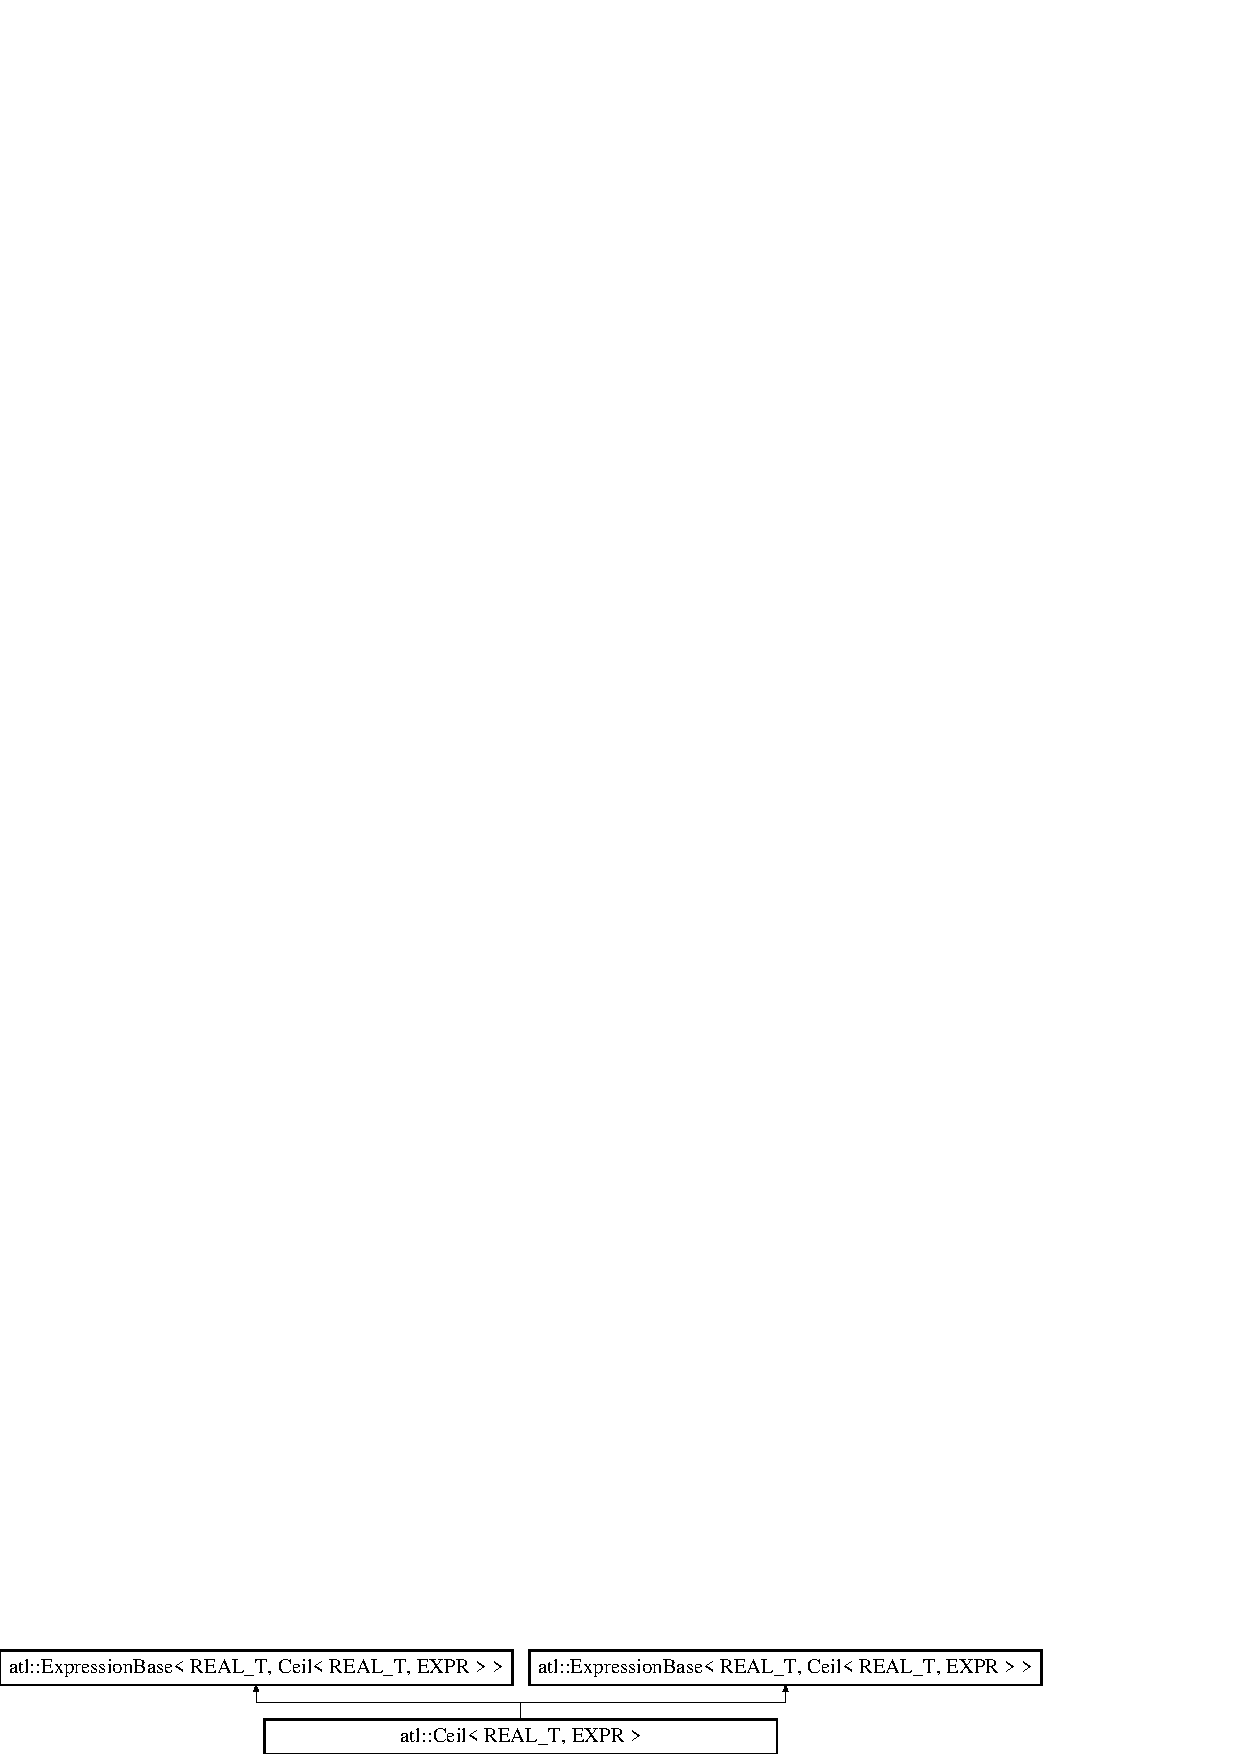
\includegraphics[height=1.637427cm]{structatl_1_1_ceil}
\end{center}
\end{figure}
\subsection*{Public Types}
\begin{DoxyCompactItemize}
\item 
\hypertarget{structatl_1_1_ceil_a464fcdf62a13706c4b9d1b66f0c40c2d}{typedef R\+E\+A\+L\+\_\+\+T {\bfseries B\+A\+S\+E\+\_\+\+T\+Y\+P\+E}}\label{structatl_1_1_ceil_a464fcdf62a13706c4b9d1b66f0c40c2d}

\item 
\hypertarget{structatl_1_1_ceil_a464fcdf62a13706c4b9d1b66f0c40c2d}{typedef R\+E\+A\+L\+\_\+\+T {\bfseries B\+A\+S\+E\+\_\+\+T\+Y\+P\+E}}\label{structatl_1_1_ceil_a464fcdf62a13706c4b9d1b66f0c40c2d}

\end{DoxyCompactItemize}
\subsection*{Public Member Functions}
\begin{DoxyCompactItemize}
\item 
\hypertarget{structatl_1_1_ceil_a77b35f66ea63f9f52445bb3bdb2ae254}{{\bfseries Ceil} (const \hyperlink{structatl_1_1_expression_base}{Expression\+Base}$<$ R\+E\+A\+L\+\_\+\+T, E\+X\+P\+R $>$ \&a)}\label{structatl_1_1_ceil_a77b35f66ea63f9f52445bb3bdb2ae254}

\item 
\hypertarget{structatl_1_1_ceil_a7a666fa878458db83fdf26675df3c977}{const R\+E\+A\+L\+\_\+\+T {\bfseries Get\+Value} () const }\label{structatl_1_1_ceil_a7a666fa878458db83fdf26675df3c977}

\item 
\hypertarget{structatl_1_1_ceil_a8191d630fa233e453bb1c9b19a82d189}{const R\+E\+A\+L\+\_\+\+T {\bfseries Get\+Value} (size\+\_\+t i, size\+\_\+t j=0) const }\label{structatl_1_1_ceil_a8191d630fa233e453bb1c9b19a82d189}

\item 
\hypertarget{structatl_1_1_ceil_a1d418e693c8e74abbc0383a0159a0b31}{void {\bfseries Push\+Ids} (typename \hyperlink{structatl_1_1_stack_entry}{atl\+::\+Stack\+Entry}$<$ R\+E\+A\+L\+\_\+\+T $>$\+::vi\+\_\+storage \&ids) const }\label{structatl_1_1_ceil_a1d418e693c8e74abbc0383a0159a0b31}

\item 
\hypertarget{structatl_1_1_ceil_a5b445cc02c0668379f8b3fdce1eac855}{void {\bfseries Push\+Ids} (typename \hyperlink{structatl_1_1_stack_entry}{atl\+::\+Stack\+Entry}$<$ R\+E\+A\+L\+\_\+\+T $>$\+::vi\+\_\+storage \&ids, size\+\_\+t i, size\+\_\+t j=0) const }\label{structatl_1_1_ceil_a5b445cc02c0668379f8b3fdce1eac855}

\item 
\hypertarget{structatl_1_1_ceil_a40b57710a46f166a8b437719fb252ab8}{const R\+E\+A\+L\+\_\+\+T {\bfseries Evaluate\+Derivative} (uint32\+\_\+t id) const }\label{structatl_1_1_ceil_a40b57710a46f166a8b437719fb252ab8}

\item 
\hypertarget{structatl_1_1_ceil_af3dcb4db885987e2b679c9583f967284}{R\+E\+A\+L\+\_\+\+T {\bfseries Evaluate\+Derivative} (uint32\+\_\+t a, uint32\+\_\+t b) const }\label{structatl_1_1_ceil_af3dcb4db885987e2b679c9583f967284}

\item 
\hypertarget{structatl_1_1_ceil_a3164f3d2a1aeca0e1ab1c2bbb6f0f2a8}{R\+E\+A\+L\+\_\+\+T {\bfseries Evaluate\+Derivative} (uint32\+\_\+t x, uint32\+\_\+t y, uint32\+\_\+t z) const }\label{structatl_1_1_ceil_a3164f3d2a1aeca0e1ab1c2bbb6f0f2a8}

\item 
\hypertarget{structatl_1_1_ceil_a27c9920ca287e5d645200e62cdad26d8}{const R\+E\+A\+L\+\_\+\+T {\bfseries Evaluate\+Derivative} (uint32\+\_\+t id, size\+\_\+t i, size\+\_\+t j=0) const }\label{structatl_1_1_ceil_a27c9920ca287e5d645200e62cdad26d8}

\item 
\hypertarget{structatl_1_1_ceil_a3f8280d066b749c47a2da402f0e6a509}{R\+E\+A\+L\+\_\+\+T {\bfseries Evaluate\+Derivative} (uint32\+\_\+t a, uint32\+\_\+t b, size\+\_\+t i, size\+\_\+t j=0) const }\label{structatl_1_1_ceil_a3f8280d066b749c47a2da402f0e6a509}

\item 
\hypertarget{structatl_1_1_ceil_a3e2406be290b04eada376b04436bd7fa}{R\+E\+A\+L\+\_\+\+T {\bfseries Evaluate\+Derivative} (uint32\+\_\+t x, uint32\+\_\+t y, uint32\+\_\+t z, size\+\_\+t i, size\+\_\+t j=0) const }\label{structatl_1_1_ceil_a3e2406be290b04eada376b04436bd7fa}

\item 
\hypertarget{structatl_1_1_ceil_a8284d110c7b3786e05e3825aac700eea}{size\+\_\+t {\bfseries Get\+Columns} () const }\label{structatl_1_1_ceil_a8284d110c7b3786e05e3825aac700eea}

\item 
\hypertarget{structatl_1_1_ceil_ada0a7f2d030572e2e4706388c0aded4a}{size\+\_\+t {\bfseries Get\+Rows} () const }\label{structatl_1_1_ceil_ada0a7f2d030572e2e4706388c0aded4a}

\item 
\hypertarget{structatl_1_1_ceil_a1e16ac8e0c238584c8f9836ef1cf176f}{bool {\bfseries Is\+Scalar} () const }\label{structatl_1_1_ceil_a1e16ac8e0c238584c8f9836ef1cf176f}

\item 
\hyperlink{structatl_1_1_ceil_a77b35f66ea63f9f52445bb3bdb2ae254}{Ceil} (const \hyperlink{structatl_1_1_expression_base}{Expression\+Base}$<$ R\+E\+A\+L\+\_\+\+T, E\+X\+P\+R $>$ \&a)
\item 
const R\+E\+A\+L\+\_\+\+T \hyperlink{structatl_1_1_ceil_a7a666fa878458db83fdf26675df3c977}{Get\+Value} () const 
\item 
const R\+E\+A\+L\+\_\+\+T \hyperlink{structatl_1_1_ceil_a8191d630fa233e453bb1c9b19a82d189}{Get\+Value} (size\+\_\+t i, size\+\_\+t j=0) const 
\item 
bool \hyperlink{structatl_1_1_ceil_aa27a1b182c49a808b0640b2ffb0198e3}{Is\+Nonlinear} () const 
\item 
void \hyperlink{structatl_1_1_ceil_a1d418e693c8e74abbc0383a0159a0b31}{Push\+Ids} (typename \hyperlink{structatl_1_1_stack_entry}{atl\+::\+Stack\+Entry}$<$ R\+E\+A\+L\+\_\+\+T $>$\+::vi\+\_\+storage \&ids) const 
\item 
void \hyperlink{structatl_1_1_ceil_a5b445cc02c0668379f8b3fdce1eac855}{Push\+Ids} (typename \hyperlink{structatl_1_1_stack_entry}{atl\+::\+Stack\+Entry}$<$ R\+E\+A\+L\+\_\+\+T $>$\+::vi\+\_\+storage \&ids, size\+\_\+t i, size\+\_\+t j=0) const 
\item 
const R\+E\+A\+L\+\_\+\+T \hyperlink{structatl_1_1_ceil_acb53a63ec3bd24e33335bef5d326ac0a}{Evaluate\+Derivative} (uint32\+\_\+t x) const 
\item 
R\+E\+A\+L\+\_\+\+T \hyperlink{structatl_1_1_ceil_a5bca6daf83b7f3e165d4c652d8e7b4e8}{Evaluate\+Derivative} (uint32\+\_\+t x, uint32\+\_\+t y) const 
\item 
R\+E\+A\+L\+\_\+\+T \hyperlink{structatl_1_1_ceil_a3164f3d2a1aeca0e1ab1c2bbb6f0f2a8}{Evaluate\+Derivative} (uint32\+\_\+t x, uint32\+\_\+t y, uint32\+\_\+t z) const 
\item 
const R\+E\+A\+L\+\_\+\+T \hyperlink{structatl_1_1_ceil_a9880875b3dab28bd33fe1f5e4d466e53}{Evaluate\+Derivative} (uint32\+\_\+t x, size\+\_\+t i, size\+\_\+t j=0) const 
\item 
R\+E\+A\+L\+\_\+\+T \hyperlink{structatl_1_1_ceil_aa2aad8819ecdb994e133e085aa20bb83}{Evaluate\+Derivative} (uint32\+\_\+t x, uint32\+\_\+t y, size\+\_\+t i, size\+\_\+t j=0) const 
\item 
R\+E\+A\+L\+\_\+\+T \hyperlink{structatl_1_1_ceil_a3e2406be290b04eada376b04436bd7fa}{Evaluate\+Derivative} (uint32\+\_\+t x, uint32\+\_\+t y, uint32\+\_\+t z, size\+\_\+t i, size\+\_\+t j=0) const 
\item 
size\+\_\+t \hyperlink{structatl_1_1_ceil_ada0a7f2d030572e2e4706388c0aded4a}{Get\+Rows} () const 
\item 
bool \hyperlink{structatl_1_1_ceil_a1e16ac8e0c238584c8f9836ef1cf176f}{Is\+Scalar} () const 
\item 
const std\+::string \hyperlink{structatl_1_1_ceil_a8f90da2fe07fc2523f845fa12d28c795}{To\+Expression\+Template\+String} () const 
\end{DoxyCompactItemize}
\subsection*{Public Attributes}
\begin{DoxyCompactItemize}
\item 
\hypertarget{structatl_1_1_ceil_a1c3766993dc3454f47e2eaf012088d9e}{const E\+X\+P\+R \& {\bfseries expr\+\_\+m}}\label{structatl_1_1_ceil_a1c3766993dc3454f47e2eaf012088d9e}

\end{DoxyCompactItemize}


\subsection{Detailed Description}
\subsubsection*{template$<$class R\+E\+A\+L\+\_\+\+T, class E\+X\+P\+R$>$struct atl\+::\+Ceil$<$ R\+E\+A\+L\+\_\+\+T, E\+X\+P\+R $>$}

Evaluate the ceiling of an expression. This template is not differentiable. 

\subsection{Constructor \& Destructor Documentation}
\hypertarget{structatl_1_1_ceil_a77b35f66ea63f9f52445bb3bdb2ae254}{\index{atl\+::\+Ceil@{atl\+::\+Ceil}!Ceil@{Ceil}}
\index{Ceil@{Ceil}!atl\+::\+Ceil@{atl\+::\+Ceil}}
\subsubsection[{Ceil}]{\setlength{\rightskip}{0pt plus 5cm}template$<$class R\+E\+A\+L\+\_\+\+T , class E\+X\+P\+R $>$ {\bf atl\+::\+Ceil}$<$ R\+E\+A\+L\+\_\+\+T, E\+X\+P\+R $>$\+::{\bf Ceil} (
\begin{DoxyParamCaption}
\item[{const {\bf Expression\+Base}$<$ R\+E\+A\+L\+\_\+\+T, E\+X\+P\+R $>$ \&}]{a}
\end{DoxyParamCaption}
)\hspace{0.3cm}{\ttfamily [inline]}}}\label{structatl_1_1_ceil_a77b35f66ea63f9f52445bb3bdb2ae254}
Constructor


\begin{DoxyParams}{Parameters}
{\em a} & \\
\hline
\end{DoxyParams}


\subsection{Member Function Documentation}
\hypertarget{structatl_1_1_ceil_acb53a63ec3bd24e33335bef5d326ac0a}{\index{atl\+::\+Ceil@{atl\+::\+Ceil}!Evaluate\+Derivative@{Evaluate\+Derivative}}
\index{Evaluate\+Derivative@{Evaluate\+Derivative}!atl\+::\+Ceil@{atl\+::\+Ceil}}
\subsubsection[{Evaluate\+Derivative}]{\setlength{\rightskip}{0pt plus 5cm}template$<$class R\+E\+A\+L\+\_\+\+T , class E\+X\+P\+R $>$ const R\+E\+A\+L\+\_\+\+T {\bf atl\+::\+Ceil}$<$ R\+E\+A\+L\+\_\+\+T, E\+X\+P\+R $>$\+::Evaluate\+Derivative (
\begin{DoxyParamCaption}
\item[{uint32\+\_\+t}]{x}
\end{DoxyParamCaption}
) const\hspace{0.3cm}{\ttfamily [inline]}}}\label{structatl_1_1_ceil_acb53a63ec3bd24e33335bef5d326ac0a}
Returns 0. Not differentiable.


\begin{DoxyParams}{Parameters}
{\em x} & \\
\hline
\end{DoxyParams}
\begin{DoxyReturn}{Returns}

\end{DoxyReturn}
\hypertarget{structatl_1_1_ceil_a5bca6daf83b7f3e165d4c652d8e7b4e8}{\index{atl\+::\+Ceil@{atl\+::\+Ceil}!Evaluate\+Derivative@{Evaluate\+Derivative}}
\index{Evaluate\+Derivative@{Evaluate\+Derivative}!atl\+::\+Ceil@{atl\+::\+Ceil}}
\subsubsection[{Evaluate\+Derivative}]{\setlength{\rightskip}{0pt plus 5cm}template$<$class R\+E\+A\+L\+\_\+\+T , class E\+X\+P\+R $>$ R\+E\+A\+L\+\_\+\+T {\bf atl\+::\+Ceil}$<$ R\+E\+A\+L\+\_\+\+T, E\+X\+P\+R $>$\+::Evaluate\+Derivative (
\begin{DoxyParamCaption}
\item[{uint32\+\_\+t}]{x, }
\item[{uint32\+\_\+t}]{y}
\end{DoxyParamCaption}
) const\hspace{0.3cm}{\ttfamily [inline]}}}\label{structatl_1_1_ceil_a5bca6daf83b7f3e165d4c652d8e7b4e8}
Returns 0. Not differentiable.


\begin{DoxyParams}{Parameters}
{\em x} & \\
\hline
{\em y} & \\
\hline
\end{DoxyParams}
\begin{DoxyReturn}{Returns}

\end{DoxyReturn}
\hypertarget{structatl_1_1_ceil_a3164f3d2a1aeca0e1ab1c2bbb6f0f2a8}{\index{atl\+::\+Ceil@{atl\+::\+Ceil}!Evaluate\+Derivative@{Evaluate\+Derivative}}
\index{Evaluate\+Derivative@{Evaluate\+Derivative}!atl\+::\+Ceil@{atl\+::\+Ceil}}
\subsubsection[{Evaluate\+Derivative}]{\setlength{\rightskip}{0pt plus 5cm}template$<$class R\+E\+A\+L\+\_\+\+T , class E\+X\+P\+R $>$ R\+E\+A\+L\+\_\+\+T {\bf atl\+::\+Ceil}$<$ R\+E\+A\+L\+\_\+\+T, E\+X\+P\+R $>$\+::Evaluate\+Derivative (
\begin{DoxyParamCaption}
\item[{uint32\+\_\+t}]{x, }
\item[{uint32\+\_\+t}]{y, }
\item[{uint32\+\_\+t}]{z}
\end{DoxyParamCaption}
) const\hspace{0.3cm}{\ttfamily [inline]}}}\label{structatl_1_1_ceil_a3164f3d2a1aeca0e1ab1c2bbb6f0f2a8}
Returns 0. Not differentiable.


\begin{DoxyParams}{Parameters}
{\em x} & \\
\hline
{\em y} & \\
\hline
{\em z} & \\
\hline
\end{DoxyParams}
\begin{DoxyReturn}{Returns}

\end{DoxyReturn}
\hypertarget{structatl_1_1_ceil_a9880875b3dab28bd33fe1f5e4d466e53}{\index{atl\+::\+Ceil@{atl\+::\+Ceil}!Evaluate\+Derivative@{Evaluate\+Derivative}}
\index{Evaluate\+Derivative@{Evaluate\+Derivative}!atl\+::\+Ceil@{atl\+::\+Ceil}}
\subsubsection[{Evaluate\+Derivative}]{\setlength{\rightskip}{0pt plus 5cm}template$<$class R\+E\+A\+L\+\_\+\+T , class E\+X\+P\+R $>$ const R\+E\+A\+L\+\_\+\+T {\bf atl\+::\+Ceil}$<$ R\+E\+A\+L\+\_\+\+T, E\+X\+P\+R $>$\+::Evaluate\+Derivative (
\begin{DoxyParamCaption}
\item[{uint32\+\_\+t}]{x, }
\item[{size\+\_\+t}]{i, }
\item[{size\+\_\+t}]{j = {\ttfamily 0}}
\end{DoxyParamCaption}
) const\hspace{0.3cm}{\ttfamily [inline]}}}\label{structatl_1_1_ceil_a9880875b3dab28bd33fe1f5e4d466e53}
Returns 0. Not differentiable.


\begin{DoxyParams}{Parameters}
{\em x} & \\
\hline
{\em i} & \\
\hline
{\em j} & \\
\hline
\end{DoxyParams}
\begin{DoxyReturn}{Returns}

\end{DoxyReturn}
\hypertarget{structatl_1_1_ceil_aa2aad8819ecdb994e133e085aa20bb83}{\index{atl\+::\+Ceil@{atl\+::\+Ceil}!Evaluate\+Derivative@{Evaluate\+Derivative}}
\index{Evaluate\+Derivative@{Evaluate\+Derivative}!atl\+::\+Ceil@{atl\+::\+Ceil}}
\subsubsection[{Evaluate\+Derivative}]{\setlength{\rightskip}{0pt plus 5cm}template$<$class R\+E\+A\+L\+\_\+\+T , class E\+X\+P\+R $>$ R\+E\+A\+L\+\_\+\+T {\bf atl\+::\+Ceil}$<$ R\+E\+A\+L\+\_\+\+T, E\+X\+P\+R $>$\+::Evaluate\+Derivative (
\begin{DoxyParamCaption}
\item[{uint32\+\_\+t}]{x, }
\item[{uint32\+\_\+t}]{y, }
\item[{size\+\_\+t}]{i, }
\item[{size\+\_\+t}]{j = {\ttfamily 0}}
\end{DoxyParamCaption}
) const\hspace{0.3cm}{\ttfamily [inline]}}}\label{structatl_1_1_ceil_aa2aad8819ecdb994e133e085aa20bb83}
Returns 0. Not differentiable. 
\begin{DoxyParams}{Parameters}
{\em x} & \\
\hline
{\em y} & \\
\hline
{\em i} & \\
\hline
{\em j} & \\
\hline
\end{DoxyParams}
\begin{DoxyReturn}{Returns}

\end{DoxyReturn}
\hypertarget{structatl_1_1_ceil_a3e2406be290b04eada376b04436bd7fa}{\index{atl\+::\+Ceil@{atl\+::\+Ceil}!Evaluate\+Derivative@{Evaluate\+Derivative}}
\index{Evaluate\+Derivative@{Evaluate\+Derivative}!atl\+::\+Ceil@{atl\+::\+Ceil}}
\subsubsection[{Evaluate\+Derivative}]{\setlength{\rightskip}{0pt plus 5cm}template$<$class R\+E\+A\+L\+\_\+\+T , class E\+X\+P\+R $>$ R\+E\+A\+L\+\_\+\+T {\bf atl\+::\+Ceil}$<$ R\+E\+A\+L\+\_\+\+T, E\+X\+P\+R $>$\+::Evaluate\+Derivative (
\begin{DoxyParamCaption}
\item[{uint32\+\_\+t}]{x, }
\item[{uint32\+\_\+t}]{y, }
\item[{uint32\+\_\+t}]{z, }
\item[{size\+\_\+t}]{i, }
\item[{size\+\_\+t}]{j = {\ttfamily 0}}
\end{DoxyParamCaption}
) const\hspace{0.3cm}{\ttfamily [inline]}}}\label{structatl_1_1_ceil_a3e2406be290b04eada376b04436bd7fa}
Returns 0. Not differentiable.


\begin{DoxyParams}{Parameters}
{\em x} & \\
\hline
{\em y} & \\
\hline
{\em z} & \\
\hline
{\em i} & \\
\hline
{\em j} & \\
\hline
\end{DoxyParams}
\begin{DoxyReturn}{Returns}

\end{DoxyReturn}
\hypertarget{structatl_1_1_ceil_ada0a7f2d030572e2e4706388c0aded4a}{\index{atl\+::\+Ceil@{atl\+::\+Ceil}!Get\+Rows@{Get\+Rows}}
\index{Get\+Rows@{Get\+Rows}!atl\+::\+Ceil@{atl\+::\+Ceil}}
\subsubsection[{Get\+Rows}]{\setlength{\rightskip}{0pt plus 5cm}template$<$class R\+E\+A\+L\+\_\+\+T , class E\+X\+P\+R $>$ size\+\_\+t {\bf atl\+::\+Ceil}$<$ R\+E\+A\+L\+\_\+\+T, E\+X\+P\+R $>$\+::Get\+Rows (
\begin{DoxyParamCaption}
{}
\end{DoxyParamCaption}
) const\hspace{0.3cm}{\ttfamily [inline]}}}\label{structatl_1_1_ceil_ada0a7f2d030572e2e4706388c0aded4a}
Return the number of rows.

\begin{DoxyReturn}{Returns}

\end{DoxyReturn}
\hypertarget{structatl_1_1_ceil_a7a666fa878458db83fdf26675df3c977}{\index{atl\+::\+Ceil@{atl\+::\+Ceil}!Get\+Value@{Get\+Value}}
\index{Get\+Value@{Get\+Value}!atl\+::\+Ceil@{atl\+::\+Ceil}}
\subsubsection[{Get\+Value}]{\setlength{\rightskip}{0pt plus 5cm}template$<$class R\+E\+A\+L\+\_\+\+T , class E\+X\+P\+R $>$ const R\+E\+A\+L\+\_\+\+T {\bf atl\+::\+Ceil}$<$ R\+E\+A\+L\+\_\+\+T, E\+X\+P\+R $>$\+::Get\+Value (
\begin{DoxyParamCaption}
{}
\end{DoxyParamCaption}
) const\hspace{0.3cm}{\ttfamily [inline]}}}\label{structatl_1_1_ceil_a7a666fa878458db83fdf26675df3c977}
Computes the ceiling of the evaluated expression.

\begin{DoxyReturn}{Returns}

\end{DoxyReturn}
\hypertarget{structatl_1_1_ceil_a8191d630fa233e453bb1c9b19a82d189}{\index{atl\+::\+Ceil@{atl\+::\+Ceil}!Get\+Value@{Get\+Value}}
\index{Get\+Value@{Get\+Value}!atl\+::\+Ceil@{atl\+::\+Ceil}}
\subsubsection[{Get\+Value}]{\setlength{\rightskip}{0pt plus 5cm}template$<$class R\+E\+A\+L\+\_\+\+T , class E\+X\+P\+R $>$ const R\+E\+A\+L\+\_\+\+T {\bf atl\+::\+Ceil}$<$ R\+E\+A\+L\+\_\+\+T, E\+X\+P\+R $>$\+::Get\+Value (
\begin{DoxyParamCaption}
\item[{size\+\_\+t}]{i, }
\item[{size\+\_\+t}]{j = {\ttfamily 0}}
\end{DoxyParamCaption}
) const\hspace{0.3cm}{\ttfamily [inline]}}}\label{structatl_1_1_ceil_a8191d630fa233e453bb1c9b19a82d189}
Computes the ceiling of the evaluated expression at index \{i,j\}.

\begin{DoxyReturn}{Returns}

\end{DoxyReturn}
\hypertarget{structatl_1_1_ceil_aa27a1b182c49a808b0640b2ffb0198e3}{\index{atl\+::\+Ceil@{atl\+::\+Ceil}!Is\+Nonlinear@{Is\+Nonlinear}}
\index{Is\+Nonlinear@{Is\+Nonlinear}!atl\+::\+Ceil@{atl\+::\+Ceil}}
\subsubsection[{Is\+Nonlinear}]{\setlength{\rightskip}{0pt plus 5cm}template$<$class R\+E\+A\+L\+\_\+\+T , class E\+X\+P\+R $>$ bool {\bf atl\+::\+Ceil}$<$ R\+E\+A\+L\+\_\+\+T, E\+X\+P\+R $>$\+::Is\+Nonlinear (
\begin{DoxyParamCaption}
{}
\end{DoxyParamCaption}
) const\hspace{0.3cm}{\ttfamily [inline]}}}\label{structatl_1_1_ceil_aa27a1b182c49a808b0640b2ffb0198e3}
Returns false.

\begin{DoxyReturn}{Returns}

\end{DoxyReturn}
\hypertarget{structatl_1_1_ceil_a1e16ac8e0c238584c8f9836ef1cf176f}{\index{atl\+::\+Ceil@{atl\+::\+Ceil}!Is\+Scalar@{Is\+Scalar}}
\index{Is\+Scalar@{Is\+Scalar}!atl\+::\+Ceil@{atl\+::\+Ceil}}
\subsubsection[{Is\+Scalar}]{\setlength{\rightskip}{0pt plus 5cm}template$<$class R\+E\+A\+L\+\_\+\+T , class E\+X\+P\+R $>$ bool {\bf atl\+::\+Ceil}$<$ R\+E\+A\+L\+\_\+\+T, E\+X\+P\+R $>$\+::Is\+Scalar (
\begin{DoxyParamCaption}
{}
\end{DoxyParamCaption}
) const\hspace{0.3cm}{\ttfamily [inline]}}}\label{structatl_1_1_ceil_a1e16ac8e0c238584c8f9836ef1cf176f}
True if this expression is a scalar.

\begin{DoxyReturn}{Returns}

\end{DoxyReturn}
\hypertarget{structatl_1_1_ceil_a1d418e693c8e74abbc0383a0159a0b31}{\index{atl\+::\+Ceil@{atl\+::\+Ceil}!Push\+Ids@{Push\+Ids}}
\index{Push\+Ids@{Push\+Ids}!atl\+::\+Ceil@{atl\+::\+Ceil}}
\subsubsection[{Push\+Ids}]{\setlength{\rightskip}{0pt plus 5cm}template$<$class R\+E\+A\+L\+\_\+\+T , class E\+X\+P\+R $>$ void {\bf atl\+::\+Ceil}$<$ R\+E\+A\+L\+\_\+\+T, E\+X\+P\+R $>$\+::Push\+Ids (
\begin{DoxyParamCaption}
\item[{typename {\bf atl\+::\+Stack\+Entry}$<$ R\+E\+A\+L\+\_\+\+T $>$\+::vi\+\_\+storage \&}]{ids}
\end{DoxyParamCaption}
) const\hspace{0.3cm}{\ttfamily [inline]}}}\label{structatl_1_1_ceil_a1d418e693c8e74abbc0383a0159a0b31}
Push variable info into a set.


\begin{DoxyParams}{Parameters}
{\em ids} & \\
\hline
{\em i} & \\
\hline
{\em j} & \\
\hline
\end{DoxyParams}
\hypertarget{structatl_1_1_ceil_a5b445cc02c0668379f8b3fdce1eac855}{\index{atl\+::\+Ceil@{atl\+::\+Ceil}!Push\+Ids@{Push\+Ids}}
\index{Push\+Ids@{Push\+Ids}!atl\+::\+Ceil@{atl\+::\+Ceil}}
\subsubsection[{Push\+Ids}]{\setlength{\rightskip}{0pt plus 5cm}template$<$class R\+E\+A\+L\+\_\+\+T , class E\+X\+P\+R $>$ void {\bf atl\+::\+Ceil}$<$ R\+E\+A\+L\+\_\+\+T, E\+X\+P\+R $>$\+::Push\+Ids (
\begin{DoxyParamCaption}
\item[{typename {\bf atl\+::\+Stack\+Entry}$<$ R\+E\+A\+L\+\_\+\+T $>$\+::vi\+\_\+storage \&}]{ids, }
\item[{size\+\_\+t}]{i, }
\item[{size\+\_\+t}]{j = {\ttfamily 0}}
\end{DoxyParamCaption}
) const\hspace{0.3cm}{\ttfamily [inline]}}}\label{structatl_1_1_ceil_a5b445cc02c0668379f8b3fdce1eac855}
Push variable info into a set at index \{i,j\}.


\begin{DoxyParams}{Parameters}
{\em ids} & \\
\hline
{\em i} & \\
\hline
{\em j} & \\
\hline
\end{DoxyParams}
\hypertarget{structatl_1_1_ceil_a8f90da2fe07fc2523f845fa12d28c795}{\index{atl\+::\+Ceil@{atl\+::\+Ceil}!To\+Expression\+Template\+String@{To\+Expression\+Template\+String}}
\index{To\+Expression\+Template\+String@{To\+Expression\+Template\+String}!atl\+::\+Ceil@{atl\+::\+Ceil}}
\subsubsection[{To\+Expression\+Template\+String}]{\setlength{\rightskip}{0pt plus 5cm}template$<$class R\+E\+A\+L\+\_\+\+T , class E\+X\+P\+R $>$ const std\+::string {\bf atl\+::\+Ceil}$<$ R\+E\+A\+L\+\_\+\+T, E\+X\+P\+R $>$\+::To\+Expression\+Template\+String (
\begin{DoxyParamCaption}
{}
\end{DoxyParamCaption}
) const\hspace{0.3cm}{\ttfamily [inline]}}}\label{structatl_1_1_ceil_a8f90da2fe07fc2523f845fa12d28c795}
Create a string representation of this expression template. \begin{DoxyReturn}{Returns}

\end{DoxyReturn}


The documentation for this struct was generated from the following file\+:\begin{DoxyCompactItemize}
\item 
A\+T\+L2/Ceil.\+hpp\end{DoxyCompactItemize}

\hypertarget{structport_1_1cilist}{\section{port\+:\+:cilist Struct Reference}
\label{structport_1_1cilist}\index{port\+::cilist@{port\+::cilist}}
}
\subsection*{Public Attributes}
\begin{DoxyCompactItemize}
\item 
\hypertarget{structport_1_1cilist_a37ef3e093cc1499d9a1c5861ff94da70}{flag {\bfseries cierr}}\label{structport_1_1cilist_a37ef3e093cc1499d9a1c5861ff94da70}

\item 
\hypertarget{structport_1_1cilist_a4e82c4880add9dd19da4b5b8fa5253f9}{ftnint {\bfseries ciunit}}\label{structport_1_1cilist_a4e82c4880add9dd19da4b5b8fa5253f9}

\item 
\hypertarget{structport_1_1cilist_a70b7a94c399007378ef31fa5026de9da}{flag {\bfseries ciend}}\label{structport_1_1cilist_a70b7a94c399007378ef31fa5026de9da}

\item 
\hypertarget{structport_1_1cilist_a12514af102d5f7c132d6e328a6764395}{char $\ast$ {\bfseries cifmt}}\label{structport_1_1cilist_a12514af102d5f7c132d6e328a6764395}

\item 
\hypertarget{structport_1_1cilist_ab341f7c9a6369780b66dac60baf48002}{ftnint {\bfseries cirec}}\label{structport_1_1cilist_ab341f7c9a6369780b66dac60baf48002}

\end{DoxyCompactItemize}


The documentation for this struct was generated from the following file\+:\begin{DoxyCompactItemize}
\item 
A\+T\+L2/support/port.\+hpp\end{DoxyCompactItemize}

\hypertarget{structatl_1_1clfallocator}{\section{atl\+:\+:clfallocator$<$ T $>$ Struct Template Reference}
\label{structatl_1_1clfallocator}\index{atl\+::clfallocator$<$ T $>$@{atl\+::clfallocator$<$ T $>$}}
}
\subsection*{Classes}
\begin{DoxyCompactItemize}
\item 
struct \hyperlink{structatl_1_1clfallocator_1_1rebind}{rebind}
\end{DoxyCompactItemize}
\subsection*{Public Types}
\begin{DoxyCompactItemize}
\item 
\hypertarget{structatl_1_1clfallocator_a34eabad415ae8479dd858e4db56ce9d9}{typedef size\+\_\+t {\bfseries size\+\_\+type}}\label{structatl_1_1clfallocator_a34eabad415ae8479dd858e4db56ce9d9}

\item 
\hypertarget{structatl_1_1clfallocator_a21249150949e0637d6d00615f3dc993e}{typedef ptrdiff\+\_\+t {\bfseries difference\+\_\+type}}\label{structatl_1_1clfallocator_a21249150949e0637d6d00615f3dc993e}

\item 
\hypertarget{structatl_1_1clfallocator_a46af2812244f29a8064dba46a8d14f05}{typedef T $\ast$ {\bfseries pointer}}\label{structatl_1_1clfallocator_a46af2812244f29a8064dba46a8d14f05}

\item 
\hypertarget{structatl_1_1clfallocator_a218d8f189fe2d6fb4f5bb8451c4ec437}{typedef const T $\ast$ {\bfseries const\+\_\+pointer}}\label{structatl_1_1clfallocator_a218d8f189fe2d6fb4f5bb8451c4ec437}

\item 
\hypertarget{structatl_1_1clfallocator_a0e470cffd8101d871a042757099b4cad}{typedef T \& {\bfseries reference}}\label{structatl_1_1clfallocator_a0e470cffd8101d871a042757099b4cad}

\item 
\hypertarget{structatl_1_1clfallocator_a35b9fb2605f611f54c0a0978f852fe40}{typedef const T \& {\bfseries const\+\_\+reference}}\label{structatl_1_1clfallocator_a35b9fb2605f611f54c0a0978f852fe40}

\item 
\hypertarget{structatl_1_1clfallocator_a205f3f994d2ec2d61f2bf3435c9267dd}{typedef T {\bfseries value\+\_\+type}}\label{structatl_1_1clfallocator_a205f3f994d2ec2d61f2bf3435c9267dd}

\item 
\hypertarget{structatl_1_1clfallocator_a34eabad415ae8479dd858e4db56ce9d9}{typedef size\+\_\+t {\bfseries size\+\_\+type}}\label{structatl_1_1clfallocator_a34eabad415ae8479dd858e4db56ce9d9}

\item 
\hypertarget{structatl_1_1clfallocator_a21249150949e0637d6d00615f3dc993e}{typedef ptrdiff\+\_\+t {\bfseries difference\+\_\+type}}\label{structatl_1_1clfallocator_a21249150949e0637d6d00615f3dc993e}

\item 
\hypertarget{structatl_1_1clfallocator_a46af2812244f29a8064dba46a8d14f05}{typedef T $\ast$ {\bfseries pointer}}\label{structatl_1_1clfallocator_a46af2812244f29a8064dba46a8d14f05}

\item 
\hypertarget{structatl_1_1clfallocator_a218d8f189fe2d6fb4f5bb8451c4ec437}{typedef const T $\ast$ {\bfseries const\+\_\+pointer}}\label{structatl_1_1clfallocator_a218d8f189fe2d6fb4f5bb8451c4ec437}

\item 
\hypertarget{structatl_1_1clfallocator_a0e470cffd8101d871a042757099b4cad}{typedef T \& {\bfseries reference}}\label{structatl_1_1clfallocator_a0e470cffd8101d871a042757099b4cad}

\item 
\hypertarget{structatl_1_1clfallocator_a35b9fb2605f611f54c0a0978f852fe40}{typedef const T \& {\bfseries const\+\_\+reference}}\label{structatl_1_1clfallocator_a35b9fb2605f611f54c0a0978f852fe40}

\item 
\hypertarget{structatl_1_1clfallocator_a205f3f994d2ec2d61f2bf3435c9267dd}{typedef T {\bfseries value\+\_\+type}}\label{structatl_1_1clfallocator_a205f3f994d2ec2d61f2bf3435c9267dd}

\item 
\hypertarget{structatl_1_1clfallocator_a34eabad415ae8479dd858e4db56ce9d9}{typedef size\+\_\+t {\bfseries size\+\_\+type}}\label{structatl_1_1clfallocator_a34eabad415ae8479dd858e4db56ce9d9}

\item 
\hypertarget{structatl_1_1clfallocator_a21249150949e0637d6d00615f3dc993e}{typedef ptrdiff\+\_\+t {\bfseries difference\+\_\+type}}\label{structatl_1_1clfallocator_a21249150949e0637d6d00615f3dc993e}

\item 
\hypertarget{structatl_1_1clfallocator_a46af2812244f29a8064dba46a8d14f05}{typedef T $\ast$ {\bfseries pointer}}\label{structatl_1_1clfallocator_a46af2812244f29a8064dba46a8d14f05}

\item 
\hypertarget{structatl_1_1clfallocator_a218d8f189fe2d6fb4f5bb8451c4ec437}{typedef const T $\ast$ {\bfseries const\+\_\+pointer}}\label{structatl_1_1clfallocator_a218d8f189fe2d6fb4f5bb8451c4ec437}

\item 
\hypertarget{structatl_1_1clfallocator_a0e470cffd8101d871a042757099b4cad}{typedef T \& {\bfseries reference}}\label{structatl_1_1clfallocator_a0e470cffd8101d871a042757099b4cad}

\item 
\hypertarget{structatl_1_1clfallocator_a35b9fb2605f611f54c0a0978f852fe40}{typedef const T \& {\bfseries const\+\_\+reference}}\label{structatl_1_1clfallocator_a35b9fb2605f611f54c0a0978f852fe40}

\item 
\hypertarget{structatl_1_1clfallocator_a205f3f994d2ec2d61f2bf3435c9267dd}{typedef T {\bfseries value\+\_\+type}}\label{structatl_1_1clfallocator_a205f3f994d2ec2d61f2bf3435c9267dd}

\end{DoxyCompactItemize}
\subsection*{Public Member Functions}
\begin{DoxyCompactItemize}
\item 
\hypertarget{structatl_1_1clfallocator_a8928d061c1c2a1dbab013e7326bb069b}{{\bfseries clfallocator} (const \hyperlink{structatl_1_1clfallocator}{clfallocator} \&)  throw ()}\label{structatl_1_1clfallocator_a8928d061c1c2a1dbab013e7326bb069b}

\item 
\hypertarget{structatl_1_1clfallocator_a1f5a58370ba67cf8a646bb86e445fc67}{{\footnotesize template$<$class U $>$ }\\{\bfseries clfallocator} (const \hyperlink{structatl_1_1clfallocator}{clfallocator}$<$ U $>$ \&)  throw ()}\label{structatl_1_1clfallocator_a1f5a58370ba67cf8a646bb86e445fc67}

\item 
\hypertarget{structatl_1_1clfallocator_a7a8b1f5f859ebc1cd1f8509ad681164c}{pointer {\bfseries address} (reference x) const }\label{structatl_1_1clfallocator_a7a8b1f5f859ebc1cd1f8509ad681164c}

\item 
\hypertarget{structatl_1_1clfallocator_a54cd719ba718b880e8a804b8734ab710}{const\+\_\+pointer {\bfseries address} (const\+\_\+reference x) const }\label{structatl_1_1clfallocator_a54cd719ba718b880e8a804b8734ab710}

\item 
\hypertarget{structatl_1_1clfallocator_aea65f52c1c20d0ebfcca437beb865a5d}{pointer {\bfseries allocate} (size\+\_\+type s, void const $\ast$=0)}\label{structatl_1_1clfallocator_aea65f52c1c20d0ebfcca437beb865a5d}

\item 
\hypertarget{structatl_1_1clfallocator_adbb84b7714c54c46cf34ca8046b444fc}{void {\bfseries deallocate} (pointer p, size\+\_\+type)}\label{structatl_1_1clfallocator_adbb84b7714c54c46cf34ca8046b444fc}

\item 
\hypertarget{structatl_1_1clfallocator_a01b57d577ebda86a68dea5d97efafff9}{size\+\_\+type {\bfseries max\+\_\+size} () const   throw ()}\label{structatl_1_1clfallocator_a01b57d577ebda86a68dea5d97efafff9}

\item 
\hypertarget{structatl_1_1clfallocator_af3fde57bd7401696b232dac995de70e2}{void {\bfseries construct} (pointer p, const T \&val)}\label{structatl_1_1clfallocator_af3fde57bd7401696b232dac995de70e2}

\item 
\hypertarget{structatl_1_1clfallocator_a98e3deb0f4af68706a8e0f1e273387bd}{void {\bfseries destroy} (pointer p)}\label{structatl_1_1clfallocator_a98e3deb0f4af68706a8e0f1e273387bd}

\item 
\hypertarget{structatl_1_1clfallocator_a8928d061c1c2a1dbab013e7326bb069b}{{\bfseries clfallocator} (const \hyperlink{structatl_1_1clfallocator}{clfallocator} \&)  throw ()}\label{structatl_1_1clfallocator_a8928d061c1c2a1dbab013e7326bb069b}

\item 
\hypertarget{structatl_1_1clfallocator_a1f5a58370ba67cf8a646bb86e445fc67}{{\footnotesize template$<$class U $>$ }\\{\bfseries clfallocator} (const \hyperlink{structatl_1_1clfallocator}{clfallocator}$<$ U $>$ \&)  throw ()}\label{structatl_1_1clfallocator_a1f5a58370ba67cf8a646bb86e445fc67}

\item 
\hypertarget{structatl_1_1clfallocator_a7a8b1f5f859ebc1cd1f8509ad681164c}{pointer {\bfseries address} (reference x) const }\label{structatl_1_1clfallocator_a7a8b1f5f859ebc1cd1f8509ad681164c}

\item 
\hypertarget{structatl_1_1clfallocator_a54cd719ba718b880e8a804b8734ab710}{const\+\_\+pointer {\bfseries address} (const\+\_\+reference x) const }\label{structatl_1_1clfallocator_a54cd719ba718b880e8a804b8734ab710}

\item 
\hypertarget{structatl_1_1clfallocator_aea65f52c1c20d0ebfcca437beb865a5d}{pointer {\bfseries allocate} (size\+\_\+type s, void const $\ast$=0)}\label{structatl_1_1clfallocator_aea65f52c1c20d0ebfcca437beb865a5d}

\item 
\hypertarget{structatl_1_1clfallocator_adbb84b7714c54c46cf34ca8046b444fc}{void {\bfseries deallocate} (pointer p, size\+\_\+type)}\label{structatl_1_1clfallocator_adbb84b7714c54c46cf34ca8046b444fc}

\item 
\hypertarget{structatl_1_1clfallocator_a01b57d577ebda86a68dea5d97efafff9}{size\+\_\+type {\bfseries max\+\_\+size} () const   throw ()}\label{structatl_1_1clfallocator_a01b57d577ebda86a68dea5d97efafff9}

\item 
\hypertarget{structatl_1_1clfallocator_af3fde57bd7401696b232dac995de70e2}{void {\bfseries construct} (pointer p, const T \&val)}\label{structatl_1_1clfallocator_af3fde57bd7401696b232dac995de70e2}

\item 
\hypertarget{structatl_1_1clfallocator_a98e3deb0f4af68706a8e0f1e273387bd}{void {\bfseries destroy} (pointer p)}\label{structatl_1_1clfallocator_a98e3deb0f4af68706a8e0f1e273387bd}

\item 
\hypertarget{structatl_1_1clfallocator_a8928d061c1c2a1dbab013e7326bb069b}{{\bfseries clfallocator} (const \hyperlink{structatl_1_1clfallocator}{clfallocator} \&)  throw ()}\label{structatl_1_1clfallocator_a8928d061c1c2a1dbab013e7326bb069b}

\item 
\hypertarget{structatl_1_1clfallocator_a1f5a58370ba67cf8a646bb86e445fc67}{{\footnotesize template$<$class U $>$ }\\{\bfseries clfallocator} (const \hyperlink{structatl_1_1clfallocator}{clfallocator}$<$ U $>$ \&)  throw ()}\label{structatl_1_1clfallocator_a1f5a58370ba67cf8a646bb86e445fc67}

\item 
\hypertarget{structatl_1_1clfallocator_a7a8b1f5f859ebc1cd1f8509ad681164c}{pointer {\bfseries address} (reference x) const }\label{structatl_1_1clfallocator_a7a8b1f5f859ebc1cd1f8509ad681164c}

\item 
\hypertarget{structatl_1_1clfallocator_a54cd719ba718b880e8a804b8734ab710}{const\+\_\+pointer {\bfseries address} (const\+\_\+reference x) const }\label{structatl_1_1clfallocator_a54cd719ba718b880e8a804b8734ab710}

\item 
\hypertarget{structatl_1_1clfallocator_aea65f52c1c20d0ebfcca437beb865a5d}{pointer {\bfseries allocate} (size\+\_\+type s, void const $\ast$=0)}\label{structatl_1_1clfallocator_aea65f52c1c20d0ebfcca437beb865a5d}

\item 
\hypertarget{structatl_1_1clfallocator_adbb84b7714c54c46cf34ca8046b444fc}{void {\bfseries deallocate} (pointer p, size\+\_\+type)}\label{structatl_1_1clfallocator_adbb84b7714c54c46cf34ca8046b444fc}

\item 
\hypertarget{structatl_1_1clfallocator_a01b57d577ebda86a68dea5d97efafff9}{size\+\_\+type {\bfseries max\+\_\+size} () const   throw ()}\label{structatl_1_1clfallocator_a01b57d577ebda86a68dea5d97efafff9}

\item 
\hypertarget{structatl_1_1clfallocator_af3fde57bd7401696b232dac995de70e2}{void {\bfseries construct} (pointer p, const T \&val)}\label{structatl_1_1clfallocator_af3fde57bd7401696b232dac995de70e2}

\item 
\hypertarget{structatl_1_1clfallocator_a98e3deb0f4af68706a8e0f1e273387bd}{void {\bfseries destroy} (pointer p)}\label{structatl_1_1clfallocator_a98e3deb0f4af68706a8e0f1e273387bd}

\end{DoxyCompactItemize}


The documentation for this struct was generated from the following file\+:\begin{DoxyCompactItemize}
\item 
A\+T\+L2/C\+L\+F\+Allocator.\+hpp\end{DoxyCompactItemize}

\hypertarget{classutil_1_1_combinations_with_repetition}{\section{util\+:\+:Combinations\+With\+Repetition Class Reference}
\label{classutil_1_1_combinations_with_repetition}\index{util\+::\+Combinations\+With\+Repetition@{util\+::\+Combinations\+With\+Repetition}}
}
\subsection*{Public Member Functions}
\begin{DoxyCompactItemize}
\item 
\hypertarget{classutil_1_1_combinations_with_repetition_a44438fef8dda93a2c3a4b8a5000e9739}{{\bfseries Combinations\+With\+Repetition} (int n, int k)}\label{classutil_1_1_combinations_with_repetition_a44438fef8dda93a2c3a4b8a5000e9739}

\item 
\hypertarget{classutil_1_1_combinations_with_repetition_a33e969d39233173d932830e9a6c9f3c6}{bool {\bfseries Next} ()}\label{classutil_1_1_combinations_with_repetition_a33e969d39233173d932830e9a6c9f3c6}

\item 
\hypertarget{classutil_1_1_combinations_with_repetition_aecc5aae1a212d6abcc8977dd28750658}{int {\bfseries operator\mbox{[}$\,$\mbox{]}} (int i)}\label{classutil_1_1_combinations_with_repetition_aecc5aae1a212d6abcc8977dd28750658}

\item 
\hypertarget{classutil_1_1_combinations_with_repetition_ac9130257a2934ab29b89b385b111b8e6}{size\+\_\+t {\bfseries Size} ()}\label{classutil_1_1_combinations_with_repetition_ac9130257a2934ab29b89b385b111b8e6}

\item 
\hypertarget{classutil_1_1_combinations_with_repetition_a5caec7287a7af4a51280b36397d78afa}{void {\bfseries Reset} (int n, int k)}\label{classutil_1_1_combinations_with_repetition_a5caec7287a7af4a51280b36397d78afa}

\end{DoxyCompactItemize}


The documentation for this class was generated from the following file\+:\begin{DoxyCompactItemize}
\item 
Utilities/Combinations.\+hpp\end{DoxyCompactItemize}

\hypertarget{classutil_1_1_combonations}{\section{util\+:\+:Combonations Class Reference}
\label{classutil_1_1_combonations}\index{util\+::\+Combonations@{util\+::\+Combonations}}
}


{\ttfamily \#include $<$Combinations.\+hpp$>$}

\subsection*{Public Member Functions}
\begin{DoxyCompactItemize}
\item 
\hypertarget{classutil_1_1_combonations_a3b8389a1e4459ccc9aa4cb40dc62dea4}{{\bfseries Combonations} (const std\+::vector$<$ int $>$ \&elems, int choose)}\label{classutil_1_1_combonations_a3b8389a1e4459ccc9aa4cb40dc62dea4}

\item 
\hypertarget{classutil_1_1_combonations_a7828c4d640f27628ca51834204ea8adf}{std\+::vector$<$ std\+::vector$<$ int $>$ $>$ \& {\bfseries Get\+Combinations} ()}\label{classutil_1_1_combonations_a7828c4d640f27628ca51834204ea8adf}

\end{DoxyCompactItemize}
\subsection*{Static Public Member Functions}
\begin{DoxyCompactItemize}
\item 
\hypertarget{classutil_1_1_combonations_ab6764d72f845b528ccb5a030a2214b97}{static void {\bfseries Create} (const std\+::vector$<$ int $>$ \&elems, unsigned long req\+\_\+len, std\+::vector$<$ std\+::vector$<$ int $>$ $>$ \&combos)}\label{classutil_1_1_combonations_ab6764d72f845b528ccb5a030a2214b97}

\end{DoxyCompactItemize}


\subsection{Detailed Description}
Simple class to create a list of combinations with repetition.


\begin{DoxyParams}{Parameters}
{\em elems} & \\
\hline
{\em req\+\_\+len} & \\
\hline
{\em pos} & \\
\hline
{\em depth} & \\
\hline
{\em margin} & \\
\hline
{\em combos} & \\
\hline
\end{DoxyParams}


The documentation for this class was generated from the following file\+:\begin{DoxyCompactItemize}
\item 
Utilities/Combinations.\+hpp\end{DoxyCompactItemize}

\hypertarget{classutil_1_1compressed__vector}{\section{util\+:\+:compressed\+\_\+vector$<$ T $>$ Class Template Reference}
\label{classutil_1_1compressed__vector}\index{util\+::compressed\+\_\+vector$<$ T $>$@{util\+::compressed\+\_\+vector$<$ T $>$}}
}
\subsection*{Public Types}
\begin{DoxyCompactItemize}
\item 
\hypertarget{classutil_1_1compressed__vector_ab206d5331ae4e6639ab6ed98bd170e81}{typedef std\+::vector$<$ std\+::pair\\*
$<$ size\+\_\+t, T $>$ $>$\+::iterator {\bfseries iterator}}\label{classutil_1_1compressed__vector_ab206d5331ae4e6639ab6ed98bd170e81}

\item 
\hypertarget{classutil_1_1compressed__vector_aad1849e24a94a8d377b238a44283d340}{typedef std\+::vector$<$ std\+::pair\\*
$<$ size\+\_\+t, T $>$\\*
 $>$\+::const\+\_\+iterator {\bfseries const\+\_\+iterator}}\label{classutil_1_1compressed__vector_aad1849e24a94a8d377b238a44283d340}

\item 
\hypertarget{classutil_1_1compressed__vector_ade8f753ef32ae793647d62774c7e918f}{typedef std\+::vector$<$ std\+::pair\\*
$<$ size\+\_\+t, T $>$\\*
 $>$\+::reverse\+\_\+iterator {\bfseries reverse\+\_\+iterator}}\label{classutil_1_1compressed__vector_ade8f753ef32ae793647d62774c7e918f}

\item 
\hypertarget{classutil_1_1compressed__vector_a658e29bf2db725bb200a45e9216171a6}{typedef std\+::vector$<$ std\+::pair\\*
$<$ size\+\_\+t, T $>$\\*
 $>$\+::const\+\_\+reverse\+\_\+iterator {\bfseries const\+\_\+reverse\+\_\+iterator}}\label{classutil_1_1compressed__vector_a658e29bf2db725bb200a45e9216171a6}

\end{DoxyCompactItemize}
\subsection*{Public Member Functions}
\begin{DoxyCompactItemize}
\item 
\hypertarget{classutil_1_1compressed__vector_a9bdc90e74fbcc24a388b88600a3e31b4}{{\bfseries compressed\+\_\+vector} (size\+\_\+t size=0)}\label{classutil_1_1compressed__vector_a9bdc90e74fbcc24a388b88600a3e31b4}

\item 
T \& \hyperlink{classutil_1_1compressed__vector_a05a64cdbbdbe84b71cea2fdf1edd3b42}{operator\mbox{[}$\,$\mbox{]}} (size\+\_\+t index)
\item 
T \& \hyperlink{classutil_1_1compressed__vector_a68900a49a6343732bd13c4275d95ddc2}{at} (size\+\_\+t index)
\item 
T \hyperlink{classutil_1_1compressed__vector_abc2315876a7c917af0b55e744c5c3e2e}{get} (size\+\_\+t index)
\item 
T \hyperlink{classutil_1_1compressed__vector_a0731dce280ad109f320e114fe4fd11d5}{operator()} (size\+\_\+t index)
\item 
\hypertarget{classutil_1_1compressed__vector_a5c3c5e443c9e6d51009d2e6b38e8b221}{void {\bfseries clear} ()}\label{classutil_1_1compressed__vector_a5c3c5e443c9e6d51009d2e6b38e8b221}

\item 
\hypertarget{classutil_1_1compressed__vector_a0a9d78c85c4fd21b2808cc101e6e4753}{size\+\_\+t {\bfseries size} ()}\label{classutil_1_1compressed__vector_a0a9d78c85c4fd21b2808cc101e6e4753}

\item 
\hypertarget{classutil_1_1compressed__vector_a02e2e2db6c609f32cd38f1034a2491ac}{void {\bfseries reserve} (size\+\_\+t size)}\label{classutil_1_1compressed__vector_a02e2e2db6c609f32cd38f1034a2491ac}

\item 
\hypertarget{classutil_1_1compressed__vector_a59ccaa4460c6f2d4a127c54391259c75}{void {\bfseries resize} (size\+\_\+t size, double factor=1)}\label{classutil_1_1compressed__vector_a59ccaa4460c6f2d4a127c54391259c75}

\item 
\hypertarget{classutil_1_1compressed__vector_ad6dee410753fe99240bd09a3e9bedef6}{iterator {\bfseries find} (size\+\_\+t index)}\label{classutil_1_1compressed__vector_ad6dee410753fe99240bd09a3e9bedef6}

\item 
\hypertarget{classutil_1_1compressed__vector_a3ce17668bcd20d9d40368e138c84125d}{iterator {\bfseries begin} ()}\label{classutil_1_1compressed__vector_a3ce17668bcd20d9d40368e138c84125d}

\item 
\hypertarget{classutil_1_1compressed__vector_a0cfae0f90d6a66251065d495cf24cce3}{const\+\_\+iterator {\bfseries begin} () const }\label{classutil_1_1compressed__vector_a0cfae0f90d6a66251065d495cf24cce3}

\item 
\hypertarget{classutil_1_1compressed__vector_a383e476ba39aecf022ea93fff0029191}{iterator {\bfseries end} ()}\label{classutil_1_1compressed__vector_a383e476ba39aecf022ea93fff0029191}

\item 
\hypertarget{classutil_1_1compressed__vector_a5c12b4566ab3beb62ba64432ece9a355}{const\+\_\+iterator {\bfseries end} () const }\label{classutil_1_1compressed__vector_a5c12b4566ab3beb62ba64432ece9a355}

\item 
\hypertarget{classutil_1_1compressed__vector_aeef112a0fb47daca6d268c1fe18a63c1}{reverse\+\_\+iterator {\bfseries rbegin} ()}\label{classutil_1_1compressed__vector_aeef112a0fb47daca6d268c1fe18a63c1}

\item 
\hypertarget{classutil_1_1compressed__vector_ae7a208a8b0fc43e1a22d327e35cb0cb9}{const\+\_\+reverse\+\_\+iterator {\bfseries rbegin} () const }\label{classutil_1_1compressed__vector_ae7a208a8b0fc43e1a22d327e35cb0cb9}

\item 
\hypertarget{classutil_1_1compressed__vector_a57d1a0739476892e4d0968e0e62d67ca}{reverse\+\_\+iterator {\bfseries rend} ()}\label{classutil_1_1compressed__vector_a57d1a0739476892e4d0968e0e62d67ca}

\item 
\hypertarget{classutil_1_1compressed__vector_a95ac73b3016c4198a277a15ad17de0ce}{const\+\_\+reverse\+\_\+iterator {\bfseries rend} () const }\label{classutil_1_1compressed__vector_a95ac73b3016c4198a277a15ad17de0ce}

\end{DoxyCompactItemize}


\subsection{Member Function Documentation}
\hypertarget{classutil_1_1compressed__vector_a68900a49a6343732bd13c4275d95ddc2}{\index{util\+::compressed\+\_\+vector@{util\+::compressed\+\_\+vector}!at@{at}}
\index{at@{at}!util\+::compressed\+\_\+vector@{util\+::compressed\+\_\+vector}}
\subsubsection[{at}]{\setlength{\rightskip}{0pt plus 5cm}template$<$typename T $>$ T\& {\bf util\+::compressed\+\_\+vector}$<$ T $>$\+::at (
\begin{DoxyParamCaption}
\item[{size\+\_\+t}]{index}
\end{DoxyParamCaption}
)\hspace{0.3cm}{\ttfamily [inline]}}}\label{classutil_1_1compressed__vector_a68900a49a6343732bd13c4275d95ddc2}
Returns a reference to a stored variable at given index. If the entry doesn't exist, it is created.


\begin{DoxyParams}{Parameters}
{\em index} & \\
\hline
\end{DoxyParams}
\begin{DoxyReturn}{Returns}

\end{DoxyReturn}
\hypertarget{classutil_1_1compressed__vector_abc2315876a7c917af0b55e744c5c3e2e}{\index{util\+::compressed\+\_\+vector@{util\+::compressed\+\_\+vector}!get@{get}}
\index{get@{get}!util\+::compressed\+\_\+vector@{util\+::compressed\+\_\+vector}}
\subsubsection[{get}]{\setlength{\rightskip}{0pt plus 5cm}template$<$typename T $>$ T {\bf util\+::compressed\+\_\+vector}$<$ T $>$\+::get (
\begin{DoxyParamCaption}
\item[{size\+\_\+t}]{index}
\end{DoxyParamCaption}
)\hspace{0.3cm}{\ttfamily [inline]}}}\label{classutil_1_1compressed__vector_abc2315876a7c917af0b55e744c5c3e2e}
Returns a value to a stored variable at given index. If the entry doesn't exist, the types default value is returned and no new entries are stored.


\begin{DoxyParams}{Parameters}
{\em index} & \\
\hline
\end{DoxyParams}
\begin{DoxyReturn}{Returns}

\end{DoxyReturn}
\hypertarget{classutil_1_1compressed__vector_a0731dce280ad109f320e114fe4fd11d5}{\index{util\+::compressed\+\_\+vector@{util\+::compressed\+\_\+vector}!operator()@{operator()}}
\index{operator()@{operator()}!util\+::compressed\+\_\+vector@{util\+::compressed\+\_\+vector}}
\subsubsection[{operator()}]{\setlength{\rightskip}{0pt plus 5cm}template$<$typename T $>$ T {\bf util\+::compressed\+\_\+vector}$<$ T $>$\+::operator() (
\begin{DoxyParamCaption}
\item[{size\+\_\+t}]{index}
\end{DoxyParamCaption}
)\hspace{0.3cm}{\ttfamily [inline]}}}\label{classutil_1_1compressed__vector_a0731dce280ad109f320e114fe4fd11d5}
Returns a value to a stored variable at given index. If the entry doesn't exist, the types default value is returned and no new entries are stored.


\begin{DoxyParams}{Parameters}
{\em index} & \\
\hline
\end{DoxyParams}
\begin{DoxyReturn}{Returns}

\end{DoxyReturn}
\hypertarget{classutil_1_1compressed__vector_a05a64cdbbdbe84b71cea2fdf1edd3b42}{\index{util\+::compressed\+\_\+vector@{util\+::compressed\+\_\+vector}!operator\mbox{[}$\,$\mbox{]}@{operator[]}}
\index{operator\mbox{[}$\,$\mbox{]}@{operator[]}!util\+::compressed\+\_\+vector@{util\+::compressed\+\_\+vector}}
\subsubsection[{operator[]}]{\setlength{\rightskip}{0pt plus 5cm}template$<$typename T $>$ T\& {\bf util\+::compressed\+\_\+vector}$<$ T $>$\+::operator\mbox{[}$\,$\mbox{]} (
\begin{DoxyParamCaption}
\item[{size\+\_\+t}]{index}
\end{DoxyParamCaption}
)\hspace{0.3cm}{\ttfamily [inline]}}}\label{classutil_1_1compressed__vector_a05a64cdbbdbe84b71cea2fdf1edd3b42}
Returns a reference to a stored variable at given index. If the entry doesn't exist, it is created.


\begin{DoxyParams}{Parameters}
{\em index} & \\
\hline
\end{DoxyParams}
\begin{DoxyReturn}{Returns}

\end{DoxyReturn}


The documentation for this class was generated from the following file\+:\begin{DoxyCompactItemize}
\item 
Utilities/compressed\+\_\+vector.\+hpp\end{DoxyCompactItemize}

\hypertarget{classemlib_1_1_hash_set_1_1const__iterator}{\section{emlib\+:\+:Hash\+Set$<$ Key\+T, Hash\+T, Comp\+T $>$\+:\+:const\+\_\+iterator Class Reference}
\label{classemlib_1_1_hash_set_1_1const__iterator}\index{emlib\+::\+Hash\+Set$<$ Key\+T, Hash\+T, Comp\+T $>$\+::const\+\_\+iterator@{emlib\+::\+Hash\+Set$<$ Key\+T, Hash\+T, Comp\+T $>$\+::const\+\_\+iterator}}
}
\subsection*{Public Types}
\begin{DoxyCompactItemize}
\item 
\hypertarget{classemlib_1_1_hash_set_1_1const__iterator_a0697f066ced6fe9662d84a7dd332a81c}{using {\bfseries iterator\+\_\+category} = std\+::forward\+\_\+iterator\+\_\+tag}\label{classemlib_1_1_hash_set_1_1const__iterator_a0697f066ced6fe9662d84a7dd332a81c}

\item 
\hypertarget{classemlib_1_1_hash_set_1_1const__iterator_a7834c66423bd4afe74b595ca3092264b}{using {\bfseries difference\+\_\+type} = size\+\_\+t}\label{classemlib_1_1_hash_set_1_1const__iterator_a7834c66423bd4afe74b595ca3092264b}

\item 
\hypertarget{classemlib_1_1_hash_set_1_1const__iterator_ac51f86dbddde2ae0d904a1049817ec31}{using {\bfseries distance\+\_\+type} = size\+\_\+t}\label{classemlib_1_1_hash_set_1_1const__iterator_ac51f86dbddde2ae0d904a1049817ec31}

\item 
\hypertarget{classemlib_1_1_hash_set_1_1const__iterator_af09ac12c4fb8863d5cc36af72406e914}{using {\bfseries value\+\_\+type} = const Key\+T}\label{classemlib_1_1_hash_set_1_1const__iterator_af09ac12c4fb8863d5cc36af72406e914}

\item 
\hypertarget{classemlib_1_1_hash_set_1_1const__iterator_a66ed12578deb21f1f9770b3f68cd1d4c}{using {\bfseries pointer} = value\+\_\+type $\ast$}\label{classemlib_1_1_hash_set_1_1const__iterator_a66ed12578deb21f1f9770b3f68cd1d4c}

\item 
\hypertarget{classemlib_1_1_hash_set_1_1const__iterator_a2e8f78010682725ecb2c66b73d652d03}{using {\bfseries reference} = value\+\_\+type \&}\label{classemlib_1_1_hash_set_1_1const__iterator_a2e8f78010682725ecb2c66b73d652d03}

\end{DoxyCompactItemize}
\subsection*{Public Member Functions}
\begin{DoxyCompactItemize}
\item 
\hypertarget{classemlib_1_1_hash_set_1_1const__iterator_a689aa7869905ced72b4fb8ce9317aedc}{{\bfseries const\+\_\+iterator} (\hyperlink{classemlib_1_1_hash_set_1_1iterator}{iterator} proto)}\label{classemlib_1_1_hash_set_1_1const__iterator_a689aa7869905ced72b4fb8ce9317aedc}

\item 
\hypertarget{classemlib_1_1_hash_set_1_1const__iterator_a144e3b6b7101e8b64362faff15c3c571}{{\bfseries const\+\_\+iterator} (const \hyperlink{classemlib_1_1_hash_set}{My\+Type} $\ast$hash\+\_\+set, size\+\_\+t bucket)}\label{classemlib_1_1_hash_set_1_1const__iterator_a144e3b6b7101e8b64362faff15c3c571}

\item 
\hypertarget{classemlib_1_1_hash_set_1_1const__iterator_ac09a6eddd4cc1c36fa3e75b6747827f8}{\hyperlink{classemlib_1_1_hash_set_1_1const__iterator}{const\+\_\+iterator} \& {\bfseries operator++} ()}\label{classemlib_1_1_hash_set_1_1const__iterator_ac09a6eddd4cc1c36fa3e75b6747827f8}

\item 
\hypertarget{classemlib_1_1_hash_set_1_1const__iterator_abadbe9b7eeadbd90268610075055d9d9}{\hyperlink{classemlib_1_1_hash_set_1_1const__iterator}{const\+\_\+iterator} {\bfseries operator++} (int)}\label{classemlib_1_1_hash_set_1_1const__iterator_abadbe9b7eeadbd90268610075055d9d9}

\item 
\hypertarget{classemlib_1_1_hash_set_1_1const__iterator_aa406989545fa6bdc8f27de3672a7412a}{reference {\bfseries operator$\ast$} () const }\label{classemlib_1_1_hash_set_1_1const__iterator_aa406989545fa6bdc8f27de3672a7412a}

\item 
\hypertarget{classemlib_1_1_hash_set_1_1const__iterator_a860733dfaf85d8945de67c2e80d72838}{pointer {\bfseries operator-\/$>$} () const }\label{classemlib_1_1_hash_set_1_1const__iterator_a860733dfaf85d8945de67c2e80d72838}

\item 
\hypertarget{classemlib_1_1_hash_set_1_1const__iterator_a38e2ff3f2342ab45c8794c6934f6297a}{bool {\bfseries operator==} (const \hyperlink{classemlib_1_1_hash_set_1_1const__iterator}{const\+\_\+iterator} \&rhs)}\label{classemlib_1_1_hash_set_1_1const__iterator_a38e2ff3f2342ab45c8794c6934f6297a}

\item 
\hypertarget{classemlib_1_1_hash_set_1_1const__iterator_a4fb89cf06ac54a4e9cdc416d26d1649c}{bool {\bfseries operator!=} (const \hyperlink{classemlib_1_1_hash_set_1_1const__iterator}{const\+\_\+iterator} \&rhs)}\label{classemlib_1_1_hash_set_1_1const__iterator_a4fb89cf06ac54a4e9cdc416d26d1649c}

\end{DoxyCompactItemize}
\subsection*{Public Attributes}
\begin{DoxyCompactItemize}
\item 
\hypertarget{classemlib_1_1_hash_set_1_1const__iterator_a92cb925ad3be61a3bfb008e2284dd128}{const \hyperlink{classemlib_1_1_hash_set}{My\+Type} $\ast$ {\bfseries \+\_\+set}}\label{classemlib_1_1_hash_set_1_1const__iterator_a92cb925ad3be61a3bfb008e2284dd128}

\item 
\hypertarget{classemlib_1_1_hash_set_1_1const__iterator_a25661afdabc86883c07b5c71ff373d03}{size\+\_\+t {\bfseries \+\_\+bucket}}\label{classemlib_1_1_hash_set_1_1const__iterator_a25661afdabc86883c07b5c71ff373d03}

\end{DoxyCompactItemize}


The documentation for this class was generated from the following file\+:\begin{DoxyCompactItemize}
\item 
third\+\_\+party/Hash\+Containers.\+hpp\end{DoxyCompactItemize}

\hypertarget{classemlib_1_1_hash_map_1_1const__iterator}{\section{emlib\+:\+:Hash\+Map$<$ Key\+T, Value\+T, Hash\+T, Comp\+T $>$\+:\+:const\+\_\+iterator Class Reference}
\label{classemlib_1_1_hash_map_1_1const__iterator}\index{emlib\+::\+Hash\+Map$<$ Key\+T, Value\+T, Hash\+T, Comp\+T $>$\+::const\+\_\+iterator@{emlib\+::\+Hash\+Map$<$ Key\+T, Value\+T, Hash\+T, Comp\+T $>$\+::const\+\_\+iterator}}
}
\subsection*{Public Types}
\begin{DoxyCompactItemize}
\item 
\hypertarget{classemlib_1_1_hash_map_1_1const__iterator_af469fd1f548a8476f0012f202a60e67f}{using {\bfseries iterator\+\_\+category} = std\+::forward\+\_\+iterator\+\_\+tag}\label{classemlib_1_1_hash_map_1_1const__iterator_af469fd1f548a8476f0012f202a60e67f}

\item 
\hypertarget{classemlib_1_1_hash_map_1_1const__iterator_a59ca7267d12bd03d8d38c77fa86960d3}{using {\bfseries difference\+\_\+type} = size\+\_\+t}\label{classemlib_1_1_hash_map_1_1const__iterator_a59ca7267d12bd03d8d38c77fa86960d3}

\item 
\hypertarget{classemlib_1_1_hash_map_1_1const__iterator_aa293e7b3ebdb5b3051066801ed076cf0}{using {\bfseries distance\+\_\+type} = size\+\_\+t}\label{classemlib_1_1_hash_map_1_1const__iterator_aa293e7b3ebdb5b3051066801ed076cf0}

\item 
\hypertarget{classemlib_1_1_hash_map_1_1const__iterator_a5e3c7317a96b61c5b5e279503af98a33}{using {\bfseries value\+\_\+type} = const std\+::pair$<$ Key\+T, Value\+T $>$}\label{classemlib_1_1_hash_map_1_1const__iterator_a5e3c7317a96b61c5b5e279503af98a33}

\item 
\hypertarget{classemlib_1_1_hash_map_1_1const__iterator_aebe0955740555cfc1596c1150a031295}{using {\bfseries pointer} = value\+\_\+type $\ast$}\label{classemlib_1_1_hash_map_1_1const__iterator_aebe0955740555cfc1596c1150a031295}

\item 
\hypertarget{classemlib_1_1_hash_map_1_1const__iterator_a8557ba89a8bf7e38ec22b31f3c610584}{using {\bfseries reference} = value\+\_\+type \&}\label{classemlib_1_1_hash_map_1_1const__iterator_a8557ba89a8bf7e38ec22b31f3c610584}

\end{DoxyCompactItemize}
\subsection*{Public Member Functions}
\begin{DoxyCompactItemize}
\item 
\hypertarget{classemlib_1_1_hash_map_1_1const__iterator_a93035081b14db505bc5d15188cead5df}{{\bfseries const\+\_\+iterator} (\hyperlink{classemlib_1_1_hash_map_1_1iterator}{iterator} proto)}\label{classemlib_1_1_hash_map_1_1const__iterator_a93035081b14db505bc5d15188cead5df}

\item 
\hypertarget{classemlib_1_1_hash_map_1_1const__iterator_ab7ce9d5de91c1874f563406226816d53}{{\bfseries const\+\_\+iterator} (const \hyperlink{classemlib_1_1_hash_map}{My\+Type} $\ast$hash\+\_\+map, size\+\_\+t bucket)}\label{classemlib_1_1_hash_map_1_1const__iterator_ab7ce9d5de91c1874f563406226816d53}

\item 
\hypertarget{classemlib_1_1_hash_map_1_1const__iterator_a15491a28e7fe8a3ae23a417965df8edc}{\hyperlink{classemlib_1_1_hash_map_1_1const__iterator}{const\+\_\+iterator} \& {\bfseries operator++} ()}\label{classemlib_1_1_hash_map_1_1const__iterator_a15491a28e7fe8a3ae23a417965df8edc}

\item 
\hypertarget{classemlib_1_1_hash_map_1_1const__iterator_ab6d4721d28c416b570ddbf14b2942060}{\hyperlink{classemlib_1_1_hash_map_1_1const__iterator}{const\+\_\+iterator} {\bfseries operator++} (int)}\label{classemlib_1_1_hash_map_1_1const__iterator_ab6d4721d28c416b570ddbf14b2942060}

\item 
\hypertarget{classemlib_1_1_hash_map_1_1const__iterator_a4dd75ed612587592c82312c5056f9584}{reference {\bfseries operator$\ast$} () const }\label{classemlib_1_1_hash_map_1_1const__iterator_a4dd75ed612587592c82312c5056f9584}

\item 
\hypertarget{classemlib_1_1_hash_map_1_1const__iterator_ae4071cc49406ce74dccb5eff6605cacb}{pointer {\bfseries operator-\/$>$} () const }\label{classemlib_1_1_hash_map_1_1const__iterator_ae4071cc49406ce74dccb5eff6605cacb}

\item 
\hypertarget{classemlib_1_1_hash_map_1_1const__iterator_a67be54e037ae3d667a9e5ad687fae45e}{bool {\bfseries operator==} (const \hyperlink{classemlib_1_1_hash_map_1_1const__iterator}{const\+\_\+iterator} \&rhs)}\label{classemlib_1_1_hash_map_1_1const__iterator_a67be54e037ae3d667a9e5ad687fae45e}

\item 
\hypertarget{classemlib_1_1_hash_map_1_1const__iterator_a6caa572844d4a2bf53a4ccbeeb24e441}{bool {\bfseries operator!=} (const \hyperlink{classemlib_1_1_hash_map_1_1const__iterator}{const\+\_\+iterator} \&rhs)}\label{classemlib_1_1_hash_map_1_1const__iterator_a6caa572844d4a2bf53a4ccbeeb24e441}

\end{DoxyCompactItemize}
\subsection*{Public Attributes}
\begin{DoxyCompactItemize}
\item 
\hypertarget{classemlib_1_1_hash_map_1_1const__iterator_aa763cf9cab329732a92f25af5617d540}{const \hyperlink{classemlib_1_1_hash_map}{My\+Type} $\ast$ {\bfseries \+\_\+map}}\label{classemlib_1_1_hash_map_1_1const__iterator_aa763cf9cab329732a92f25af5617d540}

\item 
\hypertarget{classemlib_1_1_hash_map_1_1const__iterator_a4ff5de52aaea0a1907a88c5c2d32f13d}{size\+\_\+t {\bfseries \+\_\+bucket}}\label{classemlib_1_1_hash_map_1_1const__iterator_a4ff5de52aaea0a1907a88c5c2d32f13d}

\end{DoxyCompactItemize}


The documentation for this class was generated from the following file\+:\begin{DoxyCompactItemize}
\item 
third\+\_\+party/Hash\+Containers.\+hpp\end{DoxyCompactItemize}

\hypertarget{structatl_1_1_container_trait}{\section{atl\+:\+:Container\+Trait$<$ T $>$ Struct Template Reference}
\label{structatl_1_1_container_trait}\index{atl\+::\+Container\+Trait$<$ T $>$@{atl\+::\+Container\+Trait$<$ T $>$}}
}
\subsection*{Public Member Functions}
\begin{DoxyCompactItemize}
\item 
\hypertarget{structatl_1_1_container_trait_ad88fff76b558b59ec893779fa940e58b}{{\footnotesize template$<$$>$ }\\bool {\bfseries is\+\_\+container}}\label{structatl_1_1_container_trait_ad88fff76b558b59ec893779fa940e58b}

\item 
\hypertarget{structatl_1_1_container_trait_a5b14e7dd1c0651ce1ea1ca8ec91591e9}{{\footnotesize template$<$$>$ }\\bool {\bfseries is\+\_\+container}}\label{structatl_1_1_container_trait_a5b14e7dd1c0651ce1ea1ca8ec91591e9}

\item 
\hypertarget{structatl_1_1_container_trait_a82a1bbd27ff858e8e94dc4ef6339bf57}{{\footnotesize template$<$$>$ }\\bool {\bfseries is\+\_\+container}}\label{structatl_1_1_container_trait_a82a1bbd27ff858e8e94dc4ef6339bf57}

\item 
\hypertarget{structatl_1_1_container_trait_ad88fff76b558b59ec893779fa940e58b}{{\footnotesize template$<$$>$ }\\bool {\bfseries is\+\_\+container}}\label{structatl_1_1_container_trait_ad88fff76b558b59ec893779fa940e58b}

\item 
\hypertarget{structatl_1_1_container_trait_a5b14e7dd1c0651ce1ea1ca8ec91591e9}{{\footnotesize template$<$$>$ }\\bool {\bfseries is\+\_\+container}}\label{structatl_1_1_container_trait_a5b14e7dd1c0651ce1ea1ca8ec91591e9}

\item 
\hypertarget{structatl_1_1_container_trait_a82a1bbd27ff858e8e94dc4ef6339bf57}{{\footnotesize template$<$$>$ }\\bool {\bfseries is\+\_\+container}}\label{structatl_1_1_container_trait_a82a1bbd27ff858e8e94dc4ef6339bf57}

\end{DoxyCompactItemize}
\subsection*{Static Public Attributes}
\begin{DoxyCompactItemize}
\item 
\hypertarget{structatl_1_1_container_trait_a3a7a13c226a00d1924a459a4a11e7b63}{static bool {\bfseries is\+\_\+container} = false}\label{structatl_1_1_container_trait_a3a7a13c226a00d1924a459a4a11e7b63}

\end{DoxyCompactItemize}


The documentation for this struct was generated from the following file\+:\begin{DoxyCompactItemize}
\item 
A\+T\+L2/Traits.\+hpp\end{DoxyCompactItemize}

\hypertarget{structcontrolblock__t}{\section{controlblock\+\_\+t Struct Reference}
\label{structcontrolblock__t}\index{controlblock\+\_\+t@{controlblock\+\_\+t}}
}
\subsection*{Public Attributes}
\begin{DoxyCompactItemize}
\item 
\hypertarget{structcontrolblock__t_a7eaf2b292648a87e77ba71b015f896d1}{\hyperlink{structsizeclass}{sizeclass\+\_\+t} {\bfseries sizeclass} \mbox{[}M\+A\+X\+S\+I\+Z\+E\+C\+L\+A\+S\+S\+E\+S\mbox{]}}\label{structcontrolblock__t_a7eaf2b292648a87e77ba71b015f896d1}

\item 
\hypertarget{structcontrolblock__t_a0a9fe1195ebac4cb4c1f5eb915a309d3}{\hyperlink{structprocheap}{procheap\+\_\+t} {\bfseries procheap} \mbox{[}1024\mbox{]}\mbox{[}M\+A\+X\+S\+I\+Z\+E\+C\+L\+A\+S\+S\+E\+S\mbox{]}}\label{structcontrolblock__t_a0a9fe1195ebac4cb4c1f5eb915a309d3}

\end{DoxyCompactItemize}


The documentation for this struct was generated from the following file\+:\begin{DoxyCompactItemize}
\item 
A\+T\+L2/clfmalloc.\+h\end{DoxyCompactItemize}

\hypertarget{structatl_1_1_cos}{\section{atl\+:\+:Cos$<$ R\+E\+A\+L\+\_\+\+T, E\+X\+P\+R $>$ Struct Template Reference}
\label{structatl_1_1_cos}\index{atl\+::\+Cos$<$ R\+E\+A\+L\+\_\+\+T, E\+X\+P\+R $>$@{atl\+::\+Cos$<$ R\+E\+A\+L\+\_\+\+T, E\+X\+P\+R $>$}}
}


{\ttfamily \#include $<$Cos.\+hpp$>$}

Inheritance diagram for atl\+:\+:Cos$<$ R\+E\+A\+L\+\_\+\+T, E\+X\+P\+R $>$\+:\begin{figure}[H]
\begin{center}
\leavevmode
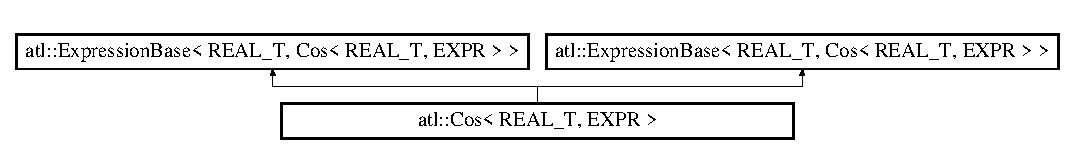
\includegraphics[height=1.637427cm]{structatl_1_1_cos}
\end{center}
\end{figure}
\subsection*{Public Types}
\begin{DoxyCompactItemize}
\item 
\hypertarget{structatl_1_1_cos_abb2ceaf23e6adb597d390e500ac15b75}{typedef R\+E\+A\+L\+\_\+\+T {\bfseries B\+A\+S\+E\+\_\+\+T\+Y\+P\+E}}\label{structatl_1_1_cos_abb2ceaf23e6adb597d390e500ac15b75}

\item 
\hypertarget{structatl_1_1_cos_abb2ceaf23e6adb597d390e500ac15b75}{typedef R\+E\+A\+L\+\_\+\+T {\bfseries B\+A\+S\+E\+\_\+\+T\+Y\+P\+E}}\label{structatl_1_1_cos_abb2ceaf23e6adb597d390e500ac15b75}

\end{DoxyCompactItemize}
\subsection*{Public Member Functions}
\begin{DoxyCompactItemize}
\item 
\hypertarget{structatl_1_1_cos_ae15e8fe45ce07f796b8e6b0f3c81a0dc}{{\bfseries Cos} (const \hyperlink{structatl_1_1_expression_base}{Expression\+Base}$<$ R\+E\+A\+L\+\_\+\+T, E\+X\+P\+R $>$ \&a)}\label{structatl_1_1_cos_ae15e8fe45ce07f796b8e6b0f3c81a0dc}

\item 
\hypertarget{structatl_1_1_cos_ace4e1b39754eac681d88a8e51777fe03}{const R\+E\+A\+L\+\_\+\+T {\bfseries Get\+Value} () const }\label{structatl_1_1_cos_ace4e1b39754eac681d88a8e51777fe03}

\item 
\hypertarget{structatl_1_1_cos_a81e3e2ea49369fe0ce486cb49501211b}{const R\+E\+A\+L\+\_\+\+T {\bfseries Get\+Value} (size\+\_\+t i, size\+\_\+t j=0) const }\label{structatl_1_1_cos_a81e3e2ea49369fe0ce486cb49501211b}

\item 
\hypertarget{structatl_1_1_cos_af1f885b1e8af4a022c3a81d901e0705c}{void {\bfseries Push\+Ids} (typename \hyperlink{structatl_1_1_stack_entry}{atl\+::\+Stack\+Entry}$<$ R\+E\+A\+L\+\_\+\+T $>$\+::vi\+\_\+storage \&ids) const }\label{structatl_1_1_cos_af1f885b1e8af4a022c3a81d901e0705c}

\item 
\hypertarget{structatl_1_1_cos_a52e381c8bab1a3e8dd59dda17f39b34b}{void {\bfseries Push\+Ids} (typename \hyperlink{structatl_1_1_stack_entry}{atl\+::\+Stack\+Entry}$<$ R\+E\+A\+L\+\_\+\+T $>$\+::vi\+\_\+storage \&ids, size\+\_\+t i, size\+\_\+t j=0) const }\label{structatl_1_1_cos_a52e381c8bab1a3e8dd59dda17f39b34b}

\item 
\hypertarget{structatl_1_1_cos_a39cf81fb9c6347e40e8d8d3efcdacdf7}{const R\+E\+A\+L\+\_\+\+T {\bfseries Evaluate\+Derivative} (uint32\+\_\+t id) const }\label{structatl_1_1_cos_a39cf81fb9c6347e40e8d8d3efcdacdf7}

\item 
\hypertarget{structatl_1_1_cos_aba2354daf666f9dd363083fea907d281}{R\+E\+A\+L\+\_\+\+T {\bfseries Evaluate\+Derivative} (uint32\+\_\+t a, uint32\+\_\+t b) const }\label{structatl_1_1_cos_aba2354daf666f9dd363083fea907d281}

\item 
\hypertarget{structatl_1_1_cos_a3daf2ee3406609a53b3d875fdf1d7a61}{R\+E\+A\+L\+\_\+\+T {\bfseries Evaluate\+Derivative} (uint32\+\_\+t x, uint32\+\_\+t y, uint32\+\_\+t z) const }\label{structatl_1_1_cos_a3daf2ee3406609a53b3d875fdf1d7a61}

\item 
\hypertarget{structatl_1_1_cos_a2655de04ccbc269b8ca0c8d61b7e2fcc}{const R\+E\+A\+L\+\_\+\+T {\bfseries Evaluate\+Derivative} (uint32\+\_\+t id, size\+\_\+t i, size\+\_\+t j=0) const }\label{structatl_1_1_cos_a2655de04ccbc269b8ca0c8d61b7e2fcc}

\item 
\hypertarget{structatl_1_1_cos_a8bd6b7e82e43213681617c8bf80c5d71}{R\+E\+A\+L\+\_\+\+T {\bfseries Evaluate\+Derivative} (uint32\+\_\+t a, uint32\+\_\+t b, size\+\_\+t i, size\+\_\+t j=0) const }\label{structatl_1_1_cos_a8bd6b7e82e43213681617c8bf80c5d71}

\item 
\hypertarget{structatl_1_1_cos_a77ec0b54497a31b2a35901ca23181641}{R\+E\+A\+L\+\_\+\+T {\bfseries Evaluate\+Derivative} (uint32\+\_\+t x, uint32\+\_\+t y, uint32\+\_\+t z, size\+\_\+t i, size\+\_\+t j=0) const }\label{structatl_1_1_cos_a77ec0b54497a31b2a35901ca23181641}

\item 
\hypertarget{structatl_1_1_cos_af5a069ad08213ab339be8fa79b634e8f}{size\+\_\+t {\bfseries Get\+Columns} () const }\label{structatl_1_1_cos_af5a069ad08213ab339be8fa79b634e8f}

\item 
\hypertarget{structatl_1_1_cos_ae2817379b49f18cbf607e1a582466878}{size\+\_\+t {\bfseries Get\+Rows} () const }\label{structatl_1_1_cos_ae2817379b49f18cbf607e1a582466878}

\item 
\hypertarget{structatl_1_1_cos_a20a3fc284b6785049cf2b2497f9b3b74}{bool {\bfseries Is\+Scalar} () const }\label{structatl_1_1_cos_a20a3fc284b6785049cf2b2497f9b3b74}

\item 
\hyperlink{structatl_1_1_cos_ae15e8fe45ce07f796b8e6b0f3c81a0dc}{Cos} (const \hyperlink{structatl_1_1_expression_base}{Expression\+Base}$<$ R\+E\+A\+L\+\_\+\+T, E\+X\+P\+R $>$ \&a)
\item 
const R\+E\+A\+L\+\_\+\+T \hyperlink{structatl_1_1_cos_ace4e1b39754eac681d88a8e51777fe03}{Get\+Value} () const 
\item 
const R\+E\+A\+L\+\_\+\+T \hyperlink{structatl_1_1_cos_a81e3e2ea49369fe0ce486cb49501211b}{Get\+Value} (size\+\_\+t i, size\+\_\+t j=0) const 
\item 
bool \hyperlink{structatl_1_1_cos_a6e00e3cfb0c28889388320143ed5892f}{Is\+Nonlinear} () const 
\item 
void \hyperlink{structatl_1_1_cos_af1f885b1e8af4a022c3a81d901e0705c}{Push\+Ids} (typename \hyperlink{structatl_1_1_stack_entry}{atl\+::\+Stack\+Entry}$<$ R\+E\+A\+L\+\_\+\+T $>$\+::vi\+\_\+storage \&ids) const 
\item 
void \hyperlink{structatl_1_1_cos_a52e381c8bab1a3e8dd59dda17f39b34b}{Push\+Ids} (typename \hyperlink{structatl_1_1_stack_entry}{atl\+::\+Stack\+Entry}$<$ R\+E\+A\+L\+\_\+\+T $>$\+::vi\+\_\+storage \&ids, size\+\_\+t i, size\+\_\+t j=0) const 
\item 
const R\+E\+A\+L\+\_\+\+T \hyperlink{structatl_1_1_cos_a0767cd6f515ac25ade8c54cacc0cd309}{Evaluate\+Derivative} (uint32\+\_\+t x) const 
\item 
R\+E\+A\+L\+\_\+\+T \hyperlink{structatl_1_1_cos_a861f527ace28cad61c0bd85665cd113a}{Evaluate\+Derivative} (uint32\+\_\+t x, uint32\+\_\+t y) const 
\item 
R\+E\+A\+L\+\_\+\+T \hyperlink{structatl_1_1_cos_a3daf2ee3406609a53b3d875fdf1d7a61}{Evaluate\+Derivative} (uint32\+\_\+t x, uint32\+\_\+t y, uint32\+\_\+t z) const 
\item 
const R\+E\+A\+L\+\_\+\+T \hyperlink{structatl_1_1_cos_a3aa481f075e1185ebb213487e164a2b0}{Evaluate\+Derivative} (uint32\+\_\+t x, size\+\_\+t i, size\+\_\+t j=0) const 
\item 
R\+E\+A\+L\+\_\+\+T \hyperlink{structatl_1_1_cos_a266a79077d99d1f824c23d538ca23266}{Evaluate\+Derivative} (uint32\+\_\+t x, uint32\+\_\+t y, size\+\_\+t i, size\+\_\+t j=0) const 
\item 
R\+E\+A\+L\+\_\+\+T \hyperlink{structatl_1_1_cos_a77ec0b54497a31b2a35901ca23181641}{Evaluate\+Derivative} (uint32\+\_\+t x, uint32\+\_\+t y, uint32\+\_\+t z, size\+\_\+t i, size\+\_\+t j=0) const 
\item 
size\+\_\+t \hyperlink{structatl_1_1_cos_af5a069ad08213ab339be8fa79b634e8f}{Get\+Columns} () const 
\item 
size\+\_\+t \hyperlink{structatl_1_1_cos_ae2817379b49f18cbf607e1a582466878}{Get\+Rows} () const 
\item 
bool \hyperlink{structatl_1_1_cos_a20a3fc284b6785049cf2b2497f9b3b74}{Is\+Scalar} () const 
\item 
const std\+::string \hyperlink{structatl_1_1_cos_af0c72d72a080a335e1d272db4fa519b5}{To\+Expression\+Template\+String} () const 
\end{DoxyCompactItemize}
\subsection*{Public Attributes}
\begin{DoxyCompactItemize}
\item 
\hypertarget{structatl_1_1_cos_aa2ef67b536d280a6c8ccced134c457ac}{const E\+X\+P\+R \& {\bfseries expr\+\_\+m}}\label{structatl_1_1_cos_aa2ef67b536d280a6c8ccced134c457ac}

\end{DoxyCompactItemize}


\subsection{Detailed Description}
\subsubsection*{template$<$class R\+E\+A\+L\+\_\+\+T, class E\+X\+P\+R$>$struct atl\+::\+Cos$<$ R\+E\+A\+L\+\_\+\+T, E\+X\+P\+R $>$}

Expression template to handle cosine for variable or container expressions.

$ \cos f(x,y) $

or

$ \cos f_{i,j}(x,y) $ 

\subsection{Constructor \& Destructor Documentation}
\hypertarget{structatl_1_1_cos_ae15e8fe45ce07f796b8e6b0f3c81a0dc}{\index{atl\+::\+Cos@{atl\+::\+Cos}!Cos@{Cos}}
\index{Cos@{Cos}!atl\+::\+Cos@{atl\+::\+Cos}}
\subsubsection[{Cos}]{\setlength{\rightskip}{0pt plus 5cm}template$<$class R\+E\+A\+L\+\_\+\+T , class E\+X\+P\+R $>$ {\bf atl\+::\+Cos}$<$ R\+E\+A\+L\+\_\+\+T, E\+X\+P\+R $>$\+::{\bf Cos} (
\begin{DoxyParamCaption}
\item[{const {\bf Expression\+Base}$<$ R\+E\+A\+L\+\_\+\+T, E\+X\+P\+R $>$ \&}]{a}
\end{DoxyParamCaption}
)\hspace{0.3cm}{\ttfamily [inline]}}}\label{structatl_1_1_cos_ae15e8fe45ce07f796b8e6b0f3c81a0dc}
Constructor.


\begin{DoxyParams}{Parameters}
{\em a} & \\
\hline
\end{DoxyParams}


\subsection{Member Function Documentation}
\hypertarget{structatl_1_1_cos_a0767cd6f515ac25ade8c54cacc0cd309}{\index{atl\+::\+Cos@{atl\+::\+Cos}!Evaluate\+Derivative@{Evaluate\+Derivative}}
\index{Evaluate\+Derivative@{Evaluate\+Derivative}!atl\+::\+Cos@{atl\+::\+Cos}}
\subsubsection[{Evaluate\+Derivative}]{\setlength{\rightskip}{0pt plus 5cm}template$<$class R\+E\+A\+L\+\_\+\+T , class E\+X\+P\+R $>$ const R\+E\+A\+L\+\_\+\+T {\bf atl\+::\+Cos}$<$ R\+E\+A\+L\+\_\+\+T, E\+X\+P\+R $>$\+::Evaluate\+Derivative (
\begin{DoxyParamCaption}
\item[{uint32\+\_\+t}]{x}
\end{DoxyParamCaption}
) const\hspace{0.3cm}{\ttfamily [inline]}}}\label{structatl_1_1_cos_a0767cd6f515ac25ade8c54cacc0cd309}
Evaluates the first-\/order derivative of this expression with respect to x.

$ -\sin f\left(x\right)\,\left({{d}\over{d\,x}}\,f\left(x\right) \right) $


\begin{DoxyParams}{Parameters}
{\em x} & \\
\hline
\end{DoxyParams}
\begin{DoxyReturn}{Returns}

\end{DoxyReturn}
\hypertarget{structatl_1_1_cos_a861f527ace28cad61c0bd85665cd113a}{\index{atl\+::\+Cos@{atl\+::\+Cos}!Evaluate\+Derivative@{Evaluate\+Derivative}}
\index{Evaluate\+Derivative@{Evaluate\+Derivative}!atl\+::\+Cos@{atl\+::\+Cos}}
\subsubsection[{Evaluate\+Derivative}]{\setlength{\rightskip}{0pt plus 5cm}template$<$class R\+E\+A\+L\+\_\+\+T , class E\+X\+P\+R $>$ R\+E\+A\+L\+\_\+\+T {\bf atl\+::\+Cos}$<$ R\+E\+A\+L\+\_\+\+T, E\+X\+P\+R $>$\+::Evaluate\+Derivative (
\begin{DoxyParamCaption}
\item[{uint32\+\_\+t}]{x, }
\item[{uint32\+\_\+t}]{y}
\end{DoxyParamCaption}
) const\hspace{0.3cm}{\ttfamily [inline]}}}\label{structatl_1_1_cos_a861f527ace28cad61c0bd85665cd113a}
Evaluates the second-\/order derivative of this expression with respect to x and y.

$ -\cos f\left(x , y\right)\,\left({{d}\over{d\,x}}\,f\left(x , y \right)\right)\,\left({{d}\over{d\,y}}\,f\left(x , y\right)\right)- \sin f\left(x , y\right)\,\left({{d^2}\over{d\,x\,d\,y}}\,f\left(x , y\right)\right) $


\begin{DoxyParams}{Parameters}
{\em x} & \\
\hline
{\em y} & \\
\hline
\end{DoxyParams}
\begin{DoxyReturn}{Returns}

\end{DoxyReturn}
\hypertarget{structatl_1_1_cos_a3daf2ee3406609a53b3d875fdf1d7a61}{\index{atl\+::\+Cos@{atl\+::\+Cos}!Evaluate\+Derivative@{Evaluate\+Derivative}}
\index{Evaluate\+Derivative@{Evaluate\+Derivative}!atl\+::\+Cos@{atl\+::\+Cos}}
\subsubsection[{Evaluate\+Derivative}]{\setlength{\rightskip}{0pt plus 5cm}template$<$class R\+E\+A\+L\+\_\+\+T , class E\+X\+P\+R $>$ R\+E\+A\+L\+\_\+\+T {\bf atl\+::\+Cos}$<$ R\+E\+A\+L\+\_\+\+T, E\+X\+P\+R $>$\+::Evaluate\+Derivative (
\begin{DoxyParamCaption}
\item[{uint32\+\_\+t}]{x, }
\item[{uint32\+\_\+t}]{y, }
\item[{uint32\+\_\+t}]{z}
\end{DoxyParamCaption}
) const\hspace{0.3cm}{\ttfamily [inline]}}}\label{structatl_1_1_cos_a3daf2ee3406609a53b3d875fdf1d7a61}
Evaluates the third-\/order derivative of this expression with respect to x, y and z.

$ \sin f\left(x , y , z\right)\,\left({{d}\over{d\,x}}\,f\left(x , y , z\right)\right)\,\left({{d}\over{d\,y}}\,f\left(x , y , z\right) \right)\,\left({{d}\over{d\,z}}\,f\left(x , y , z\right)\right)- \cos f\left(x , y , z\right)\,\left({{d^2}\over{d\,x\,d\,y}}\,f \left(x , y , z\right)\right)\,\left({{d}\over{d\,z}}\,f\left(x , y , z\right)\right)- \\ \cos f\left(x , y , z\right)\,\left({{d}\over{d\, x}}\,f\left(x , y , z\right)\right)\,\left({{d^2}\over{d\,y\,d\,z}} \,f\left(x , y , z\right)\right)-\cos f\left(x , y , z\right)\, \left({{d^2}\over{d\,x\,d\,z}}\,f\left(x , y , z\right)\right)\, \left({{d}\over{d\,y}}\,f\left(x , y , z\right)\right)-\sin f\left(x , y , z\right)\,\left({{d^3}\over{d\,x\,d\,y\,d\,z}}\,f\left(x , y , z\right)\right) $


\begin{DoxyParams}{Parameters}
{\em x} & \\
\hline
{\em y} & \\
\hline
{\em z} & \\
\hline
\end{DoxyParams}
\begin{DoxyReturn}{Returns}

\end{DoxyReturn}
\hypertarget{structatl_1_1_cos_a3aa481f075e1185ebb213487e164a2b0}{\index{atl\+::\+Cos@{atl\+::\+Cos}!Evaluate\+Derivative@{Evaluate\+Derivative}}
\index{Evaluate\+Derivative@{Evaluate\+Derivative}!atl\+::\+Cos@{atl\+::\+Cos}}
\subsubsection[{Evaluate\+Derivative}]{\setlength{\rightskip}{0pt plus 5cm}template$<$class R\+E\+A\+L\+\_\+\+T , class E\+X\+P\+R $>$ const R\+E\+A\+L\+\_\+\+T {\bf atl\+::\+Cos}$<$ R\+E\+A\+L\+\_\+\+T, E\+X\+P\+R $>$\+::Evaluate\+Derivative (
\begin{DoxyParamCaption}
\item[{uint32\+\_\+t}]{x, }
\item[{size\+\_\+t}]{i, }
\item[{size\+\_\+t}]{j = {\ttfamily 0}}
\end{DoxyParamCaption}
) const\hspace{0.3cm}{\ttfamily [inline]}}}\label{structatl_1_1_cos_a3aa481f075e1185ebb213487e164a2b0}
Evaluates the first-\/order derivative of this expression with respect to x at index \{i,j\}.

$ -\sin f_{i,j}(x)\,\left({{d}\over{d\,x}}\,f_{i,j}(x)\right)$


\begin{DoxyParams}{Parameters}
{\em x} & \\
\hline
{\em i} & \\
\hline
{\em j} & \\
\hline
\end{DoxyParams}
\begin{DoxyReturn}{Returns}

\end{DoxyReturn}
\hypertarget{structatl_1_1_cos_a266a79077d99d1f824c23d538ca23266}{\index{atl\+::\+Cos@{atl\+::\+Cos}!Evaluate\+Derivative@{Evaluate\+Derivative}}
\index{Evaluate\+Derivative@{Evaluate\+Derivative}!atl\+::\+Cos@{atl\+::\+Cos}}
\subsubsection[{Evaluate\+Derivative}]{\setlength{\rightskip}{0pt plus 5cm}template$<$class R\+E\+A\+L\+\_\+\+T , class E\+X\+P\+R $>$ R\+E\+A\+L\+\_\+\+T {\bf atl\+::\+Cos}$<$ R\+E\+A\+L\+\_\+\+T, E\+X\+P\+R $>$\+::Evaluate\+Derivative (
\begin{DoxyParamCaption}
\item[{uint32\+\_\+t}]{x, }
\item[{uint32\+\_\+t}]{y, }
\item[{size\+\_\+t}]{i, }
\item[{size\+\_\+t}]{j = {\ttfamily 0}}
\end{DoxyParamCaption}
) const\hspace{0.3cm}{\ttfamily [inline]}}}\label{structatl_1_1_cos_a266a79077d99d1f824c23d538ca23266}
Evaluates the second-\/order derivative of this expression with respect to x and y at index \{i,j\}.


\begin{DoxyParams}{Parameters}
{\em x} & \\
\hline
{\em y} & \\
\hline
{\em i} & \\
\hline
{\em j} & \\
\hline
\end{DoxyParams}
\begin{DoxyReturn}{Returns}

\end{DoxyReturn}
\hypertarget{structatl_1_1_cos_a77ec0b54497a31b2a35901ca23181641}{\index{atl\+::\+Cos@{atl\+::\+Cos}!Evaluate\+Derivative@{Evaluate\+Derivative}}
\index{Evaluate\+Derivative@{Evaluate\+Derivative}!atl\+::\+Cos@{atl\+::\+Cos}}
\subsubsection[{Evaluate\+Derivative}]{\setlength{\rightskip}{0pt plus 5cm}template$<$class R\+E\+A\+L\+\_\+\+T , class E\+X\+P\+R $>$ R\+E\+A\+L\+\_\+\+T {\bf atl\+::\+Cos}$<$ R\+E\+A\+L\+\_\+\+T, E\+X\+P\+R $>$\+::Evaluate\+Derivative (
\begin{DoxyParamCaption}
\item[{uint32\+\_\+t}]{x, }
\item[{uint32\+\_\+t}]{y, }
\item[{uint32\+\_\+t}]{z, }
\item[{size\+\_\+t}]{i, }
\item[{size\+\_\+t}]{j = {\ttfamily 0}}
\end{DoxyParamCaption}
) const\hspace{0.3cm}{\ttfamily [inline]}}}\label{structatl_1_1_cos_a77ec0b54497a31b2a35901ca23181641}
Evaluates the third-\/order derivative of this expression with respect to x, y and z at index \{i,i\}.

$ \sin f_{i,j}(x,y,z)\,\left({{d}\over{d\,x}}\,f_{i,j}(x,y,z)\right) \,\left({{d}\over{d\,y}}\,f_{i,j}(x,y,z)\right)\,\left({{d}\over{d\, z}}\,f_{i,j}(x,y,z)\right)-\cos f_{i,j}(x,y,z)\,\left({{d^2}\over{d \,x\,d\,y}}\,f_{i,j}(x,y,z)\right)\,\left({{d}\over{d\,z}}\,f_{i,j}( x,y,z)\right)- \\ \cos f_{i,j}(x,y,z)\,\left({{d}\over{d\,x}}\,f_{i,j}(x ,y,z)\right)\,\left({{d^2}\over{d\,y\,d\,z}}\,f_{i,j}(x,y,z)\right)- \cos f_{i,j}(x,y,z)\,\left({{d^2}\over{d\,x\,d\,z}}\,f_{i,j}(x,y,z) \right)\,\left({{d}\over{d\,y}}\,f_{i,j}(x,y,z)\right)-\sin f_{i,j}( x,y,z)\,\left({{d^3}\over{d\,x\,d\,y\,d\,z}}\,f_{i,j}(x,y,z)\right)$


\begin{DoxyParams}{Parameters}
{\em x} & \\
\hline
{\em y} & \\
\hline
{\em z} & \\
\hline
{\em i} & \\
\hline
{\em j} & \\
\hline
\end{DoxyParams}
\begin{DoxyReturn}{Returns}

\end{DoxyReturn}
\hypertarget{structatl_1_1_cos_af5a069ad08213ab339be8fa79b634e8f}{\index{atl\+::\+Cos@{atl\+::\+Cos}!Get\+Columns@{Get\+Columns}}
\index{Get\+Columns@{Get\+Columns}!atl\+::\+Cos@{atl\+::\+Cos}}
\subsubsection[{Get\+Columns}]{\setlength{\rightskip}{0pt plus 5cm}template$<$class R\+E\+A\+L\+\_\+\+T , class E\+X\+P\+R $>$ size\+\_\+t {\bf atl\+::\+Cos}$<$ R\+E\+A\+L\+\_\+\+T, E\+X\+P\+R $>$\+::Get\+Columns (
\begin{DoxyParamCaption}
{}
\end{DoxyParamCaption}
) const\hspace{0.3cm}{\ttfamily [inline]}}}\label{structatl_1_1_cos_af5a069ad08213ab339be8fa79b634e8f}
Return the number of columns.

\begin{DoxyReturn}{Returns}

\end{DoxyReturn}
\hypertarget{structatl_1_1_cos_ae2817379b49f18cbf607e1a582466878}{\index{atl\+::\+Cos@{atl\+::\+Cos}!Get\+Rows@{Get\+Rows}}
\index{Get\+Rows@{Get\+Rows}!atl\+::\+Cos@{atl\+::\+Cos}}
\subsubsection[{Get\+Rows}]{\setlength{\rightskip}{0pt plus 5cm}template$<$class R\+E\+A\+L\+\_\+\+T , class E\+X\+P\+R $>$ size\+\_\+t {\bf atl\+::\+Cos}$<$ R\+E\+A\+L\+\_\+\+T, E\+X\+P\+R $>$\+::Get\+Rows (
\begin{DoxyParamCaption}
{}
\end{DoxyParamCaption}
) const\hspace{0.3cm}{\ttfamily [inline]}}}\label{structatl_1_1_cos_ae2817379b49f18cbf607e1a582466878}
Return the number of rows.

\begin{DoxyReturn}{Returns}

\end{DoxyReturn}
\hypertarget{structatl_1_1_cos_ace4e1b39754eac681d88a8e51777fe03}{\index{atl\+::\+Cos@{atl\+::\+Cos}!Get\+Value@{Get\+Value}}
\index{Get\+Value@{Get\+Value}!atl\+::\+Cos@{atl\+::\+Cos}}
\subsubsection[{Get\+Value}]{\setlength{\rightskip}{0pt plus 5cm}template$<$class R\+E\+A\+L\+\_\+\+T , class E\+X\+P\+R $>$ const R\+E\+A\+L\+\_\+\+T {\bf atl\+::\+Cos}$<$ R\+E\+A\+L\+\_\+\+T, E\+X\+P\+R $>$\+::Get\+Value (
\begin{DoxyParamCaption}
{}
\end{DoxyParamCaption}
) const\hspace{0.3cm}{\ttfamily [inline]}}}\label{structatl_1_1_cos_ace4e1b39754eac681d88a8e51777fe03}
Computes the cosine of the evaluated expression.

\begin{DoxyReturn}{Returns}

\end{DoxyReturn}
\hypertarget{structatl_1_1_cos_a81e3e2ea49369fe0ce486cb49501211b}{\index{atl\+::\+Cos@{atl\+::\+Cos}!Get\+Value@{Get\+Value}}
\index{Get\+Value@{Get\+Value}!atl\+::\+Cos@{atl\+::\+Cos}}
\subsubsection[{Get\+Value}]{\setlength{\rightskip}{0pt plus 5cm}template$<$class R\+E\+A\+L\+\_\+\+T , class E\+X\+P\+R $>$ const R\+E\+A\+L\+\_\+\+T {\bf atl\+::\+Cos}$<$ R\+E\+A\+L\+\_\+\+T, E\+X\+P\+R $>$\+::Get\+Value (
\begin{DoxyParamCaption}
\item[{size\+\_\+t}]{i, }
\item[{size\+\_\+t}]{j = {\ttfamily 0}}
\end{DoxyParamCaption}
) const\hspace{0.3cm}{\ttfamily [inline]}}}\label{structatl_1_1_cos_a81e3e2ea49369fe0ce486cb49501211b}
Computes the cosine of the evaluated expression at index \{i,j\}.

\begin{DoxyReturn}{Returns}

\end{DoxyReturn}
\hypertarget{structatl_1_1_cos_a6e00e3cfb0c28889388320143ed5892f}{\index{atl\+::\+Cos@{atl\+::\+Cos}!Is\+Nonlinear@{Is\+Nonlinear}}
\index{Is\+Nonlinear@{Is\+Nonlinear}!atl\+::\+Cos@{atl\+::\+Cos}}
\subsubsection[{Is\+Nonlinear}]{\setlength{\rightskip}{0pt plus 5cm}template$<$class R\+E\+A\+L\+\_\+\+T , class E\+X\+P\+R $>$ bool {\bf atl\+::\+Cos}$<$ R\+E\+A\+L\+\_\+\+T, E\+X\+P\+R $>$\+::Is\+Nonlinear (
\begin{DoxyParamCaption}
{}
\end{DoxyParamCaption}
) const\hspace{0.3cm}{\ttfamily [inline]}}}\label{structatl_1_1_cos_a6e00e3cfb0c28889388320143ed5892f}
Returns true.

\begin{DoxyReturn}{Returns}

\end{DoxyReturn}
\hypertarget{structatl_1_1_cos_a20a3fc284b6785049cf2b2497f9b3b74}{\index{atl\+::\+Cos@{atl\+::\+Cos}!Is\+Scalar@{Is\+Scalar}}
\index{Is\+Scalar@{Is\+Scalar}!atl\+::\+Cos@{atl\+::\+Cos}}
\subsubsection[{Is\+Scalar}]{\setlength{\rightskip}{0pt plus 5cm}template$<$class R\+E\+A\+L\+\_\+\+T , class E\+X\+P\+R $>$ bool {\bf atl\+::\+Cos}$<$ R\+E\+A\+L\+\_\+\+T, E\+X\+P\+R $>$\+::Is\+Scalar (
\begin{DoxyParamCaption}
{}
\end{DoxyParamCaption}
) const\hspace{0.3cm}{\ttfamily [inline]}}}\label{structatl_1_1_cos_a20a3fc284b6785049cf2b2497f9b3b74}
True if this expression is a scalar.

\begin{DoxyReturn}{Returns}

\end{DoxyReturn}
\hypertarget{structatl_1_1_cos_af1f885b1e8af4a022c3a81d901e0705c}{\index{atl\+::\+Cos@{atl\+::\+Cos}!Push\+Ids@{Push\+Ids}}
\index{Push\+Ids@{Push\+Ids}!atl\+::\+Cos@{atl\+::\+Cos}}
\subsubsection[{Push\+Ids}]{\setlength{\rightskip}{0pt plus 5cm}template$<$class R\+E\+A\+L\+\_\+\+T , class E\+X\+P\+R $>$ void {\bf atl\+::\+Cos}$<$ R\+E\+A\+L\+\_\+\+T, E\+X\+P\+R $>$\+::Push\+Ids (
\begin{DoxyParamCaption}
\item[{typename {\bf atl\+::\+Stack\+Entry}$<$ R\+E\+A\+L\+\_\+\+T $>$\+::vi\+\_\+storage \&}]{ids}
\end{DoxyParamCaption}
) const\hspace{0.3cm}{\ttfamily [inline]}}}\label{structatl_1_1_cos_af1f885b1e8af4a022c3a81d901e0705c}
Push variable info into a set.


\begin{DoxyParams}{Parameters}
{\em ids} & \\
\hline
\end{DoxyParams}
\hypertarget{structatl_1_1_cos_a52e381c8bab1a3e8dd59dda17f39b34b}{\index{atl\+::\+Cos@{atl\+::\+Cos}!Push\+Ids@{Push\+Ids}}
\index{Push\+Ids@{Push\+Ids}!atl\+::\+Cos@{atl\+::\+Cos}}
\subsubsection[{Push\+Ids}]{\setlength{\rightskip}{0pt plus 5cm}template$<$class R\+E\+A\+L\+\_\+\+T , class E\+X\+P\+R $>$ void {\bf atl\+::\+Cos}$<$ R\+E\+A\+L\+\_\+\+T, E\+X\+P\+R $>$\+::Push\+Ids (
\begin{DoxyParamCaption}
\item[{typename {\bf atl\+::\+Stack\+Entry}$<$ R\+E\+A\+L\+\_\+\+T $>$\+::vi\+\_\+storage \&}]{ids, }
\item[{size\+\_\+t}]{i, }
\item[{size\+\_\+t}]{j = {\ttfamily 0}}
\end{DoxyParamCaption}
) const\hspace{0.3cm}{\ttfamily [inline]}}}\label{structatl_1_1_cos_a52e381c8bab1a3e8dd59dda17f39b34b}
Push variable info into a set at index \{i,j\}.


\begin{DoxyParams}{Parameters}
{\em ids} & \\
\hline
{\em i} & \\
\hline
{\em j} & \\
\hline
\end{DoxyParams}
\hypertarget{structatl_1_1_cos_af0c72d72a080a335e1d272db4fa519b5}{\index{atl\+::\+Cos@{atl\+::\+Cos}!To\+Expression\+Template\+String@{To\+Expression\+Template\+String}}
\index{To\+Expression\+Template\+String@{To\+Expression\+Template\+String}!atl\+::\+Cos@{atl\+::\+Cos}}
\subsubsection[{To\+Expression\+Template\+String}]{\setlength{\rightskip}{0pt plus 5cm}template$<$class R\+E\+A\+L\+\_\+\+T , class E\+X\+P\+R $>$ const std\+::string {\bf atl\+::\+Cos}$<$ R\+E\+A\+L\+\_\+\+T, E\+X\+P\+R $>$\+::To\+Expression\+Template\+String (
\begin{DoxyParamCaption}
{}
\end{DoxyParamCaption}
) const\hspace{0.3cm}{\ttfamily [inline]}}}\label{structatl_1_1_cos_af0c72d72a080a335e1d272db4fa519b5}
Create a string representation of this expression template. \begin{DoxyReturn}{Returns}

\end{DoxyReturn}


The documentation for this struct was generated from the following file\+:\begin{DoxyCompactItemize}
\item 
A\+T\+L2/Cos.\+hpp\end{DoxyCompactItemize}

\hypertarget{structatl_1_1_cosh}{\section{atl\+:\+:Cosh$<$ R\+E\+A\+L\+\_\+\+T, E\+X\+P\+R $>$ Struct Template Reference}
\label{structatl_1_1_cosh}\index{atl\+::\+Cosh$<$ R\+E\+A\+L\+\_\+\+T, E\+X\+P\+R $>$@{atl\+::\+Cosh$<$ R\+E\+A\+L\+\_\+\+T, E\+X\+P\+R $>$}}
}


{\ttfamily \#include $<$Cosh.\+hpp$>$}

Inheritance diagram for atl\+:\+:Cosh$<$ R\+E\+A\+L\+\_\+\+T, E\+X\+P\+R $>$\+:\begin{figure}[H]
\begin{center}
\leavevmode
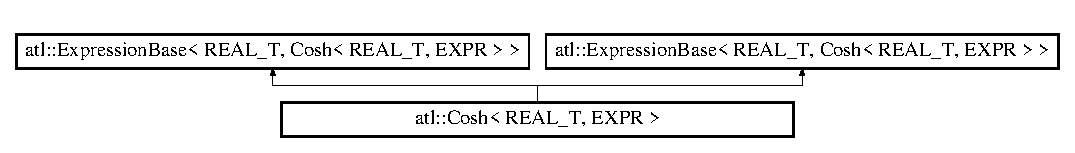
\includegraphics[height=1.604584cm]{structatl_1_1_cosh}
\end{center}
\end{figure}
\subsection*{Public Types}
\begin{DoxyCompactItemize}
\item 
\hypertarget{structatl_1_1_cosh_ab1e4552d7a61ab9bd55f6b2ca9120b89}{typedef R\+E\+A\+L\+\_\+\+T {\bfseries B\+A\+S\+E\+\_\+\+T\+Y\+P\+E}}\label{structatl_1_1_cosh_ab1e4552d7a61ab9bd55f6b2ca9120b89}

\item 
\hypertarget{structatl_1_1_cosh_ab1e4552d7a61ab9bd55f6b2ca9120b89}{typedef R\+E\+A\+L\+\_\+\+T {\bfseries B\+A\+S\+E\+\_\+\+T\+Y\+P\+E}}\label{structatl_1_1_cosh_ab1e4552d7a61ab9bd55f6b2ca9120b89}

\end{DoxyCompactItemize}
\subsection*{Public Member Functions}
\begin{DoxyCompactItemize}
\item 
\hypertarget{structatl_1_1_cosh_a01f70e880c5b34f0b1c3fe53cc81cf25}{{\bfseries Cosh} (const \hyperlink{structatl_1_1_expression_base}{Expression\+Base}$<$ R\+E\+A\+L\+\_\+\+T, E\+X\+P\+R $>$ \&a)}\label{structatl_1_1_cosh_a01f70e880c5b34f0b1c3fe53cc81cf25}

\item 
\hypertarget{structatl_1_1_cosh_a5d27569743cf020d80776454bd20b09a}{const R\+E\+A\+L\+\_\+\+T {\bfseries Get\+Value} () const }\label{structatl_1_1_cosh_a5d27569743cf020d80776454bd20b09a}

\item 
\hypertarget{structatl_1_1_cosh_a0fed96ec2f9c805a0263e6ad8fee2024}{const R\+E\+A\+L\+\_\+\+T {\bfseries Get\+Value} (size\+\_\+t i, size\+\_\+t j=0) const }\label{structatl_1_1_cosh_a0fed96ec2f9c805a0263e6ad8fee2024}

\item 
\hypertarget{structatl_1_1_cosh_a017597730da76a5672f98de2c44e2ea1}{void {\bfseries Push\+Ids} (typename \hyperlink{structatl_1_1_stack_entry}{atl\+::\+Stack\+Entry}$<$ R\+E\+A\+L\+\_\+\+T $>$\+::vi\+\_\+storage \&ids) const }\label{structatl_1_1_cosh_a017597730da76a5672f98de2c44e2ea1}

\item 
\hypertarget{structatl_1_1_cosh_aa4dde595aa26d6b04c3fa5992bc5698e}{void {\bfseries Push\+Ids} (typename \hyperlink{structatl_1_1_stack_entry}{atl\+::\+Stack\+Entry}$<$ R\+E\+A\+L\+\_\+\+T $>$\+::vi\+\_\+storage \&ids, size\+\_\+t i, size\+\_\+t j=0) const }\label{structatl_1_1_cosh_aa4dde595aa26d6b04c3fa5992bc5698e}

\item 
\hypertarget{structatl_1_1_cosh_ab1abc64106a6deb29bd071d25754a20c}{const R\+E\+A\+L\+\_\+\+T {\bfseries Evaluate\+Derivative} (uint32\+\_\+t id) const }\label{structatl_1_1_cosh_ab1abc64106a6deb29bd071d25754a20c}

\item 
\hypertarget{structatl_1_1_cosh_aee0067fbe6daa89a626b935940de0776}{R\+E\+A\+L\+\_\+\+T {\bfseries Evaluate\+Derivative} (uint32\+\_\+t a, uint32\+\_\+t b) const }\label{structatl_1_1_cosh_aee0067fbe6daa89a626b935940de0776}

\item 
\hypertarget{structatl_1_1_cosh_ab8393c0bbe1606f3a7e6b4a5d4429090}{R\+E\+A\+L\+\_\+\+T {\bfseries Evaluate\+Derivative} (uint32\+\_\+t x, uint32\+\_\+t y, uint32\+\_\+t z) const }\label{structatl_1_1_cosh_ab8393c0bbe1606f3a7e6b4a5d4429090}

\item 
\hypertarget{structatl_1_1_cosh_aa88ee8778012c6711bf51965fd6e042e}{const R\+E\+A\+L\+\_\+\+T {\bfseries Evaluate\+Derivative} (uint32\+\_\+t id, size\+\_\+t i, size\+\_\+t j=0) const }\label{structatl_1_1_cosh_aa88ee8778012c6711bf51965fd6e042e}

\item 
\hypertarget{structatl_1_1_cosh_a0a251ce5487cbab7e9bceedc1c7b8168}{R\+E\+A\+L\+\_\+\+T {\bfseries Evaluate\+Derivative} (uint32\+\_\+t a, uint32\+\_\+t b, size\+\_\+t i, size\+\_\+t j=0) const }\label{structatl_1_1_cosh_a0a251ce5487cbab7e9bceedc1c7b8168}

\item 
\hypertarget{structatl_1_1_cosh_ad5168fb3efbe6ce65f4794ffd471a166}{R\+E\+A\+L\+\_\+\+T {\bfseries Evaluate\+Derivative} (uint32\+\_\+t x, uint32\+\_\+t y, uint32\+\_\+t z, size\+\_\+t i, size\+\_\+t j=0) const }\label{structatl_1_1_cosh_ad5168fb3efbe6ce65f4794ffd471a166}

\item 
\hypertarget{structatl_1_1_cosh_acce74e20fa213340265fdde3a7e5b0fe}{size\+\_\+t {\bfseries Get\+Columns} () const }\label{structatl_1_1_cosh_acce74e20fa213340265fdde3a7e5b0fe}

\item 
\hypertarget{structatl_1_1_cosh_a058c010882bbb34bba5da54bdbe3452b}{size\+\_\+t {\bfseries Get\+Rows} () const }\label{structatl_1_1_cosh_a058c010882bbb34bba5da54bdbe3452b}

\item 
\hypertarget{structatl_1_1_cosh_a1e7bcad2334937ddb37d14773a6086d7}{bool {\bfseries Is\+Scalar} () const }\label{structatl_1_1_cosh_a1e7bcad2334937ddb37d14773a6086d7}

\item 
\hyperlink{structatl_1_1_cosh_a01f70e880c5b34f0b1c3fe53cc81cf25}{Cosh} (const \hyperlink{structatl_1_1_expression_base}{Expression\+Base}$<$ R\+E\+A\+L\+\_\+\+T, E\+X\+P\+R $>$ \&a)
\item 
const R\+E\+A\+L\+\_\+\+T \hyperlink{structatl_1_1_cosh_a5d27569743cf020d80776454bd20b09a}{Get\+Value} () const 
\item 
const R\+E\+A\+L\+\_\+\+T \hyperlink{structatl_1_1_cosh_a0fed96ec2f9c805a0263e6ad8fee2024}{Get\+Value} (size\+\_\+t i, size\+\_\+t j=0) const 
\item 
bool \hyperlink{structatl_1_1_cosh_adf2314cfd3f1b82820fe27eb2fd0849a}{Is\+Nonlinear} () const 
\item 
void \hyperlink{structatl_1_1_cosh_a017597730da76a5672f98de2c44e2ea1}{Push\+Ids} (typename \hyperlink{structatl_1_1_stack_entry}{atl\+::\+Stack\+Entry}$<$ R\+E\+A\+L\+\_\+\+T $>$\+::vi\+\_\+storage \&ids) const 
\item 
void \hyperlink{structatl_1_1_cosh_aa4dde595aa26d6b04c3fa5992bc5698e}{Push\+Ids} (typename \hyperlink{structatl_1_1_stack_entry}{atl\+::\+Stack\+Entry}$<$ R\+E\+A\+L\+\_\+\+T $>$\+::vi\+\_\+storage \&ids, size\+\_\+t i, size\+\_\+t j=0) const 
\item 
const R\+E\+A\+L\+\_\+\+T \hyperlink{structatl_1_1_cosh_a16543cbae7297561b9f11bea8026829a}{Evaluate\+Derivative} (uint32\+\_\+t x) const 
\item 
R\+E\+A\+L\+\_\+\+T \hyperlink{structatl_1_1_cosh_affc49ebbe26c43e86f83078af0c08c96}{Evaluate\+Derivative} (uint32\+\_\+t x, uint32\+\_\+t y) const 
\item 
R\+E\+A\+L\+\_\+\+T \hyperlink{structatl_1_1_cosh_ab8393c0bbe1606f3a7e6b4a5d4429090}{Evaluate\+Derivative} (uint32\+\_\+t x, uint32\+\_\+t y, uint32\+\_\+t z) const 
\item 
const R\+E\+A\+L\+\_\+\+T \hyperlink{structatl_1_1_cosh_aadbdc94b4ff2f19c1b888e32143c5266}{Evaluate\+Derivative} (uint32\+\_\+t x, size\+\_\+t i, size\+\_\+t j=0) const 
\item 
R\+E\+A\+L\+\_\+\+T \hyperlink{structatl_1_1_cosh_a57fa6b5b7d9e79206af3bf5bce579920}{Evaluate\+Derivative} (uint32\+\_\+t x, uint32\+\_\+t y, size\+\_\+t i, size\+\_\+t j=0) const 
\item 
R\+E\+A\+L\+\_\+\+T \hyperlink{structatl_1_1_cosh_ad5168fb3efbe6ce65f4794ffd471a166}{Evaluate\+Derivative} (uint32\+\_\+t x, uint32\+\_\+t y, uint32\+\_\+t z, size\+\_\+t i, size\+\_\+t j=0) const 
\item 
size\+\_\+t \hyperlink{structatl_1_1_cosh_acce74e20fa213340265fdde3a7e5b0fe}{Get\+Columns} () const 
\item 
size\+\_\+t \hyperlink{structatl_1_1_cosh_a058c010882bbb34bba5da54bdbe3452b}{Get\+Rows} () const 
\item 
bool \hyperlink{structatl_1_1_cosh_a1e7bcad2334937ddb37d14773a6086d7}{Is\+Scalar} () const 
\item 
const std\+::string \hyperlink{structatl_1_1_cosh_a142b32ec1f1d0d2dab6e504b986b4446}{To\+Expression\+Template\+String} () const 
\end{DoxyCompactItemize}
\subsection*{Public Attributes}
\begin{DoxyCompactItemize}
\item 
\hypertarget{structatl_1_1_cosh_a3a8a6bb5e513144d53fd5ed453ada881}{const E\+X\+P\+R \& {\bfseries expr\+\_\+m}}\label{structatl_1_1_cosh_a3a8a6bb5e513144d53fd5ed453ada881}

\end{DoxyCompactItemize}


\subsection{Detailed Description}
\subsubsection*{template$<$class R\+E\+A\+L\+\_\+\+T, class E\+X\+P\+R$>$struct atl\+::\+Cosh$<$ R\+E\+A\+L\+\_\+\+T, E\+X\+P\+R $>$}

Expression template to handle hyperbolic cosine for variable or container expressions.

$ \cosh f(x,y) $

or

$ \cosh f_{i,j}(x,y) $ 

\subsection{Constructor \& Destructor Documentation}
\hypertarget{structatl_1_1_cosh_a01f70e880c5b34f0b1c3fe53cc81cf25}{\index{atl\+::\+Cosh@{atl\+::\+Cosh}!Cosh@{Cosh}}
\index{Cosh@{Cosh}!atl\+::\+Cosh@{atl\+::\+Cosh}}
\subsubsection[{Cosh}]{\setlength{\rightskip}{0pt plus 5cm}template$<$class R\+E\+A\+L\+\_\+\+T , class E\+X\+P\+R $>$ {\bf atl\+::\+Cosh}$<$ R\+E\+A\+L\+\_\+\+T, E\+X\+P\+R $>$\+::{\bf Cosh} (
\begin{DoxyParamCaption}
\item[{const {\bf Expression\+Base}$<$ R\+E\+A\+L\+\_\+\+T, E\+X\+P\+R $>$ \&}]{a}
\end{DoxyParamCaption}
)\hspace{0.3cm}{\ttfamily [inline]}}}\label{structatl_1_1_cosh_a01f70e880c5b34f0b1c3fe53cc81cf25}
Constructor.


\begin{DoxyParams}{Parameters}
{\em a} & \\
\hline
\end{DoxyParams}


\subsection{Member Function Documentation}
\hypertarget{structatl_1_1_cosh_a16543cbae7297561b9f11bea8026829a}{\index{atl\+::\+Cosh@{atl\+::\+Cosh}!Evaluate\+Derivative@{Evaluate\+Derivative}}
\index{Evaluate\+Derivative@{Evaluate\+Derivative}!atl\+::\+Cosh@{atl\+::\+Cosh}}
\subsubsection[{Evaluate\+Derivative}]{\setlength{\rightskip}{0pt plus 5cm}template$<$class R\+E\+A\+L\+\_\+\+T , class E\+X\+P\+R $>$ const R\+E\+A\+L\+\_\+\+T {\bf atl\+::\+Cosh}$<$ R\+E\+A\+L\+\_\+\+T, E\+X\+P\+R $>$\+::Evaluate\+Derivative (
\begin{DoxyParamCaption}
\item[{uint32\+\_\+t}]{x}
\end{DoxyParamCaption}
) const\hspace{0.3cm}{\ttfamily [inline]}}}\label{structatl_1_1_cosh_a16543cbae7297561b9f11bea8026829a}
Evaluates the first-\/order derivative of this expression with respect to x.

$ \sinh f(x)\,\left({{d}\over{d\,x}}\,f(x)\right)$


\begin{DoxyParams}{Parameters}
{\em x} & \\
\hline
{\em i} & \\
\hline
{\em j} & \\
\hline
\end{DoxyParams}
\begin{DoxyReturn}{Returns}

\end{DoxyReturn}
\hypertarget{structatl_1_1_cosh_affc49ebbe26c43e86f83078af0c08c96}{\index{atl\+::\+Cosh@{atl\+::\+Cosh}!Evaluate\+Derivative@{Evaluate\+Derivative}}
\index{Evaluate\+Derivative@{Evaluate\+Derivative}!atl\+::\+Cosh@{atl\+::\+Cosh}}
\subsubsection[{Evaluate\+Derivative}]{\setlength{\rightskip}{0pt plus 5cm}template$<$class R\+E\+A\+L\+\_\+\+T , class E\+X\+P\+R $>$ R\+E\+A\+L\+\_\+\+T {\bf atl\+::\+Cosh}$<$ R\+E\+A\+L\+\_\+\+T, E\+X\+P\+R $>$\+::Evaluate\+Derivative (
\begin{DoxyParamCaption}
\item[{uint32\+\_\+t}]{x, }
\item[{uint32\+\_\+t}]{y}
\end{DoxyParamCaption}
) const\hspace{0.3cm}{\ttfamily [inline]}}}\label{structatl_1_1_cosh_affc49ebbe26c43e86f83078af0c08c96}
Evaluates the second-\/order derivative of this expression with respect to x and y.

$ \cosh f\left(x , y\right)\,\left({{d}\over{d\,x}}\,f\left(x , y \right)\right)\,\left({{d}\over{d\,y}}\,f\left(x , y\right)\right)+ \sinh f\left(x , y\right)\,\left({{d^2}\over{d\,x\,d\,y}}\,f\left(x , y\right)\right)$


\begin{DoxyParams}{Parameters}
{\em x} & \\
\hline
{\em y} & \\
\hline
\end{DoxyParams}
\begin{DoxyReturn}{Returns}

\end{DoxyReturn}
\hypertarget{structatl_1_1_cosh_ab8393c0bbe1606f3a7e6b4a5d4429090}{\index{atl\+::\+Cosh@{atl\+::\+Cosh}!Evaluate\+Derivative@{Evaluate\+Derivative}}
\index{Evaluate\+Derivative@{Evaluate\+Derivative}!atl\+::\+Cosh@{atl\+::\+Cosh}}
\subsubsection[{Evaluate\+Derivative}]{\setlength{\rightskip}{0pt plus 5cm}template$<$class R\+E\+A\+L\+\_\+\+T , class E\+X\+P\+R $>$ R\+E\+A\+L\+\_\+\+T {\bf atl\+::\+Cosh}$<$ R\+E\+A\+L\+\_\+\+T, E\+X\+P\+R $>$\+::Evaluate\+Derivative (
\begin{DoxyParamCaption}
\item[{uint32\+\_\+t}]{x, }
\item[{uint32\+\_\+t}]{y, }
\item[{uint32\+\_\+t}]{z}
\end{DoxyParamCaption}
) const\hspace{0.3cm}{\ttfamily [inline]}}}\label{structatl_1_1_cosh_ab8393c0bbe1606f3a7e6b4a5d4429090}
Evaluates the third-\/order derivative of this expression with respect to x, y and z.

$ \sinh f\left(x , y , z\right)\,\left({{d}\over{d\,x}}\,f\left(x , y , z\right)\right)\,\left({{d}\over{d\,y}}\,f\left(x , y , z\right) \right)\,\left({{d}\over{d\,z}}\,f\left(x , y , z\right)\right)+ \cosh f\left(x , y , z\right)\,\left({{d^2}\over{d\,x\,d\,y}}\,f \left(x , y , z\right)\right)\,\left({{d}\over{d\,z}}\,f\left(x , y , z\right)\right)+\cosh f\left(x , y , z\right)\,\left({{d}\over{d \,x}}\,f\left(x , y , z\right)\right)\,\left({{d^2}\over{d\,y\,d\,z }}\,f\left(x , y , z\right)\right)+\cosh f\left(x , y , z\right)\, \left({{d^2}\over{d\,x\,d\,z}}\,f\left(x , y , z\right)\right)\, \left({{d}\over{d\,y}}\,f\left(x , y , z\right)\right)+\sinh f\left( x , y , z\right)\,\left({{d^3}\over{d\,x\,d\,y\,d\,z}}\,f\left(x , y , z\right)\right) $


\begin{DoxyParams}{Parameters}
{\em x} & \\
\hline
{\em y} & \\
\hline
{\em z} & \\
\hline
\end{DoxyParams}
\begin{DoxyReturn}{Returns}

\end{DoxyReturn}
\hypertarget{structatl_1_1_cosh_aadbdc94b4ff2f19c1b888e32143c5266}{\index{atl\+::\+Cosh@{atl\+::\+Cosh}!Evaluate\+Derivative@{Evaluate\+Derivative}}
\index{Evaluate\+Derivative@{Evaluate\+Derivative}!atl\+::\+Cosh@{atl\+::\+Cosh}}
\subsubsection[{Evaluate\+Derivative}]{\setlength{\rightskip}{0pt plus 5cm}template$<$class R\+E\+A\+L\+\_\+\+T , class E\+X\+P\+R $>$ const R\+E\+A\+L\+\_\+\+T {\bf atl\+::\+Cosh}$<$ R\+E\+A\+L\+\_\+\+T, E\+X\+P\+R $>$\+::Evaluate\+Derivative (
\begin{DoxyParamCaption}
\item[{uint32\+\_\+t}]{x, }
\item[{size\+\_\+t}]{i, }
\item[{size\+\_\+t}]{j = {\ttfamily 0}}
\end{DoxyParamCaption}
) const\hspace{0.3cm}{\ttfamily [inline]}}}\label{structatl_1_1_cosh_aadbdc94b4ff2f19c1b888e32143c5266}
Evaluates the first-\/order derivative of this expression with respect to x at index \{i,i\}.

$ \sinh f_{i,j}(x)\,\left({{d}\over{d\,x}}\,f_{i,j}(x)\right)$


\begin{DoxyParams}{Parameters}
{\em x} & \\
\hline
{\em i} & \\
\hline
{\em j} & \\
\hline
\end{DoxyParams}
\begin{DoxyReturn}{Returns}

\end{DoxyReturn}
\hypertarget{structatl_1_1_cosh_a57fa6b5b7d9e79206af3bf5bce579920}{\index{atl\+::\+Cosh@{atl\+::\+Cosh}!Evaluate\+Derivative@{Evaluate\+Derivative}}
\index{Evaluate\+Derivative@{Evaluate\+Derivative}!atl\+::\+Cosh@{atl\+::\+Cosh}}
\subsubsection[{Evaluate\+Derivative}]{\setlength{\rightskip}{0pt plus 5cm}template$<$class R\+E\+A\+L\+\_\+\+T , class E\+X\+P\+R $>$ R\+E\+A\+L\+\_\+\+T {\bf atl\+::\+Cosh}$<$ R\+E\+A\+L\+\_\+\+T, E\+X\+P\+R $>$\+::Evaluate\+Derivative (
\begin{DoxyParamCaption}
\item[{uint32\+\_\+t}]{x, }
\item[{uint32\+\_\+t}]{y, }
\item[{size\+\_\+t}]{i, }
\item[{size\+\_\+t}]{j = {\ttfamily 0}}
\end{DoxyParamCaption}
) const\hspace{0.3cm}{\ttfamily [inline]}}}\label{structatl_1_1_cosh_a57fa6b5b7d9e79206af3bf5bce579920}
Evaluates the second-\/order derivative of this expression with respect to x and y at index \{i,i\}.

$ \cosh f_{i,j}(x,y)\,\left({{d}\over{d\,x}}\,f_{i,j}(x,y)\right)\, \left({{d}\over{d\,y}}\,f_{i,j}(x,y)\right)+\sinh f_{i,j}(x,y)\, \left({{d^2}\over{d\,x\,d\,y}}\,f_{i,j}(x,y)\right) $


\begin{DoxyParams}{Parameters}
{\em x} & \\
\hline
{\em y} & \\
\hline
{\em i} & \\
\hline
{\em j} & \\
\hline
\end{DoxyParams}
\begin{DoxyReturn}{Returns}

\end{DoxyReturn}
\hypertarget{structatl_1_1_cosh_ad5168fb3efbe6ce65f4794ffd471a166}{\index{atl\+::\+Cosh@{atl\+::\+Cosh}!Evaluate\+Derivative@{Evaluate\+Derivative}}
\index{Evaluate\+Derivative@{Evaluate\+Derivative}!atl\+::\+Cosh@{atl\+::\+Cosh}}
\subsubsection[{Evaluate\+Derivative}]{\setlength{\rightskip}{0pt plus 5cm}template$<$class R\+E\+A\+L\+\_\+\+T , class E\+X\+P\+R $>$ R\+E\+A\+L\+\_\+\+T {\bf atl\+::\+Cosh}$<$ R\+E\+A\+L\+\_\+\+T, E\+X\+P\+R $>$\+::Evaluate\+Derivative (
\begin{DoxyParamCaption}
\item[{uint32\+\_\+t}]{x, }
\item[{uint32\+\_\+t}]{y, }
\item[{uint32\+\_\+t}]{z, }
\item[{size\+\_\+t}]{i, }
\item[{size\+\_\+t}]{j = {\ttfamily 0}}
\end{DoxyParamCaption}
) const\hspace{0.3cm}{\ttfamily [inline]}}}\label{structatl_1_1_cosh_ad5168fb3efbe6ce65f4794ffd471a166}
Evaluates the third-\/order derivative of this expression with respect to x, y and z at index \{i,i\}.

$ \sinh f_{i,j}(x,y,z)\,\left({{d}\over{d\,x}}\,f_{i,j}(x,y,z)\right) \,\left({{d}\over{d\,y}}\,f_{i,j}(x,y,z)\right)\,\left({{d}\over{d\, z}}\,f_{i,j}(x,y,z)\right)+\cosh f_{i,j}(x,y,z)\,\left({{d^2}\over{d \,x\,d\,y}}\,f_{i,j}(x,y,z)\right)\,\left({{d}\over{d\,z}}\,f_{i,j}( x,y,z)\right)+ \\ \cosh f_{i,j}(x,y,z)\,\left({{d}\over{d\,x}}\,f_{i,j}( x,y,z)\right)\,\left({{d^2}\over{d\,y\,d\,z}}\,f_{i,j}(x,y,z)\right) +\cosh f_{i,j}(x,y,z)\,\left({{d^2}\over{d\,x\,d\,z}}\,f_{i,j}(x,y,z )\right)\,\left({{d}\over{d\,y}}\,f_{i,j}(x,y,z)\right)+\sinh f_{i,j }(x,y,z)\,\left({{d^3}\over{d\,x\,d\,y\,d\,z}}\,f_{i,j}(x,y,z) \right) $


\begin{DoxyParams}{Parameters}
{\em x} & \\
\hline
{\em y} & \\
\hline
{\em z} & \\
\hline
{\em i} & \\
\hline
{\em j} & \\
\hline
\end{DoxyParams}
\begin{DoxyReturn}{Returns}

\end{DoxyReturn}
\hypertarget{structatl_1_1_cosh_acce74e20fa213340265fdde3a7e5b0fe}{\index{atl\+::\+Cosh@{atl\+::\+Cosh}!Get\+Columns@{Get\+Columns}}
\index{Get\+Columns@{Get\+Columns}!atl\+::\+Cosh@{atl\+::\+Cosh}}
\subsubsection[{Get\+Columns}]{\setlength{\rightskip}{0pt plus 5cm}template$<$class R\+E\+A\+L\+\_\+\+T , class E\+X\+P\+R $>$ size\+\_\+t {\bf atl\+::\+Cosh}$<$ R\+E\+A\+L\+\_\+\+T, E\+X\+P\+R $>$\+::Get\+Columns (
\begin{DoxyParamCaption}
{}
\end{DoxyParamCaption}
) const\hspace{0.3cm}{\ttfamily [inline]}}}\label{structatl_1_1_cosh_acce74e20fa213340265fdde3a7e5b0fe}
Return the number of columns.

\begin{DoxyReturn}{Returns}

\end{DoxyReturn}
\hypertarget{structatl_1_1_cosh_a058c010882bbb34bba5da54bdbe3452b}{\index{atl\+::\+Cosh@{atl\+::\+Cosh}!Get\+Rows@{Get\+Rows}}
\index{Get\+Rows@{Get\+Rows}!atl\+::\+Cosh@{atl\+::\+Cosh}}
\subsubsection[{Get\+Rows}]{\setlength{\rightskip}{0pt plus 5cm}template$<$class R\+E\+A\+L\+\_\+\+T , class E\+X\+P\+R $>$ size\+\_\+t {\bf atl\+::\+Cosh}$<$ R\+E\+A\+L\+\_\+\+T, E\+X\+P\+R $>$\+::Get\+Rows (
\begin{DoxyParamCaption}
{}
\end{DoxyParamCaption}
) const\hspace{0.3cm}{\ttfamily [inline]}}}\label{structatl_1_1_cosh_a058c010882bbb34bba5da54bdbe3452b}
Return the number of rows.

\begin{DoxyReturn}{Returns}

\end{DoxyReturn}
\hypertarget{structatl_1_1_cosh_a5d27569743cf020d80776454bd20b09a}{\index{atl\+::\+Cosh@{atl\+::\+Cosh}!Get\+Value@{Get\+Value}}
\index{Get\+Value@{Get\+Value}!atl\+::\+Cosh@{atl\+::\+Cosh}}
\subsubsection[{Get\+Value}]{\setlength{\rightskip}{0pt plus 5cm}template$<$class R\+E\+A\+L\+\_\+\+T , class E\+X\+P\+R $>$ const R\+E\+A\+L\+\_\+\+T {\bf atl\+::\+Cosh}$<$ R\+E\+A\+L\+\_\+\+T, E\+X\+P\+R $>$\+::Get\+Value (
\begin{DoxyParamCaption}
{}
\end{DoxyParamCaption}
) const\hspace{0.3cm}{\ttfamily [inline]}}}\label{structatl_1_1_cosh_a5d27569743cf020d80776454bd20b09a}
Computes the hyperbolic cosine of the evaluated expression.

\begin{DoxyReturn}{Returns}

\end{DoxyReturn}
\hypertarget{structatl_1_1_cosh_a0fed96ec2f9c805a0263e6ad8fee2024}{\index{atl\+::\+Cosh@{atl\+::\+Cosh}!Get\+Value@{Get\+Value}}
\index{Get\+Value@{Get\+Value}!atl\+::\+Cosh@{atl\+::\+Cosh}}
\subsubsection[{Get\+Value}]{\setlength{\rightskip}{0pt plus 5cm}template$<$class R\+E\+A\+L\+\_\+\+T , class E\+X\+P\+R $>$ const R\+E\+A\+L\+\_\+\+T {\bf atl\+::\+Cosh}$<$ R\+E\+A\+L\+\_\+\+T, E\+X\+P\+R $>$\+::Get\+Value (
\begin{DoxyParamCaption}
\item[{size\+\_\+t}]{i, }
\item[{size\+\_\+t}]{j = {\ttfamily 0}}
\end{DoxyParamCaption}
) const\hspace{0.3cm}{\ttfamily [inline]}}}\label{structatl_1_1_cosh_a0fed96ec2f9c805a0263e6ad8fee2024}
Computes the hyperbolic cosine of the evaluated expression at index \{i,j\}.

\begin{DoxyReturn}{Returns}

\end{DoxyReturn}
\hypertarget{structatl_1_1_cosh_adf2314cfd3f1b82820fe27eb2fd0849a}{\index{atl\+::\+Cosh@{atl\+::\+Cosh}!Is\+Nonlinear@{Is\+Nonlinear}}
\index{Is\+Nonlinear@{Is\+Nonlinear}!atl\+::\+Cosh@{atl\+::\+Cosh}}
\subsubsection[{Is\+Nonlinear}]{\setlength{\rightskip}{0pt plus 5cm}template$<$class R\+E\+A\+L\+\_\+\+T , class E\+X\+P\+R $>$ bool {\bf atl\+::\+Cosh}$<$ R\+E\+A\+L\+\_\+\+T, E\+X\+P\+R $>$\+::Is\+Nonlinear (
\begin{DoxyParamCaption}
{}
\end{DoxyParamCaption}
) const\hspace{0.3cm}{\ttfamily [inline]}}}\label{structatl_1_1_cosh_adf2314cfd3f1b82820fe27eb2fd0849a}
Returns true.

\begin{DoxyReturn}{Returns}

\end{DoxyReturn}
\hypertarget{structatl_1_1_cosh_a1e7bcad2334937ddb37d14773a6086d7}{\index{atl\+::\+Cosh@{atl\+::\+Cosh}!Is\+Scalar@{Is\+Scalar}}
\index{Is\+Scalar@{Is\+Scalar}!atl\+::\+Cosh@{atl\+::\+Cosh}}
\subsubsection[{Is\+Scalar}]{\setlength{\rightskip}{0pt plus 5cm}template$<$class R\+E\+A\+L\+\_\+\+T , class E\+X\+P\+R $>$ bool {\bf atl\+::\+Cosh}$<$ R\+E\+A\+L\+\_\+\+T, E\+X\+P\+R $>$\+::Is\+Scalar (
\begin{DoxyParamCaption}
{}
\end{DoxyParamCaption}
) const\hspace{0.3cm}{\ttfamily [inline]}}}\label{structatl_1_1_cosh_a1e7bcad2334937ddb37d14773a6086d7}
True if this expression is a scalar.

\begin{DoxyReturn}{Returns}

\end{DoxyReturn}
\hypertarget{structatl_1_1_cosh_a017597730da76a5672f98de2c44e2ea1}{\index{atl\+::\+Cosh@{atl\+::\+Cosh}!Push\+Ids@{Push\+Ids}}
\index{Push\+Ids@{Push\+Ids}!atl\+::\+Cosh@{atl\+::\+Cosh}}
\subsubsection[{Push\+Ids}]{\setlength{\rightskip}{0pt plus 5cm}template$<$class R\+E\+A\+L\+\_\+\+T , class E\+X\+P\+R $>$ void {\bf atl\+::\+Cosh}$<$ R\+E\+A\+L\+\_\+\+T, E\+X\+P\+R $>$\+::Push\+Ids (
\begin{DoxyParamCaption}
\item[{typename {\bf atl\+::\+Stack\+Entry}$<$ R\+E\+A\+L\+\_\+\+T $>$\+::vi\+\_\+storage \&}]{ids}
\end{DoxyParamCaption}
) const\hspace{0.3cm}{\ttfamily [inline]}}}\label{structatl_1_1_cosh_a017597730da76a5672f98de2c44e2ea1}
Push variable info into a set.


\begin{DoxyParams}{Parameters}
{\em ids} & \\
\hline
{\em i} & \\
\hline
{\em j} & \\
\hline
\end{DoxyParams}
\hypertarget{structatl_1_1_cosh_aa4dde595aa26d6b04c3fa5992bc5698e}{\index{atl\+::\+Cosh@{atl\+::\+Cosh}!Push\+Ids@{Push\+Ids}}
\index{Push\+Ids@{Push\+Ids}!atl\+::\+Cosh@{atl\+::\+Cosh}}
\subsubsection[{Push\+Ids}]{\setlength{\rightskip}{0pt plus 5cm}template$<$class R\+E\+A\+L\+\_\+\+T , class E\+X\+P\+R $>$ void {\bf atl\+::\+Cosh}$<$ R\+E\+A\+L\+\_\+\+T, E\+X\+P\+R $>$\+::Push\+Ids (
\begin{DoxyParamCaption}
\item[{typename {\bf atl\+::\+Stack\+Entry}$<$ R\+E\+A\+L\+\_\+\+T $>$\+::vi\+\_\+storage \&}]{ids, }
\item[{size\+\_\+t}]{i, }
\item[{size\+\_\+t}]{j = {\ttfamily 0}}
\end{DoxyParamCaption}
) const\hspace{0.3cm}{\ttfamily [inline]}}}\label{structatl_1_1_cosh_aa4dde595aa26d6b04c3fa5992bc5698e}
Push variable info into a set at index \{i,j\}.


\begin{DoxyParams}{Parameters}
{\em ids} & \\
\hline
{\em i} & \\
\hline
{\em j} & \\
\hline
\end{DoxyParams}
\hypertarget{structatl_1_1_cosh_a142b32ec1f1d0d2dab6e504b986b4446}{\index{atl\+::\+Cosh@{atl\+::\+Cosh}!To\+Expression\+Template\+String@{To\+Expression\+Template\+String}}
\index{To\+Expression\+Template\+String@{To\+Expression\+Template\+String}!atl\+::\+Cosh@{atl\+::\+Cosh}}
\subsubsection[{To\+Expression\+Template\+String}]{\setlength{\rightskip}{0pt plus 5cm}template$<$class R\+E\+A\+L\+\_\+\+T , class E\+X\+P\+R $>$ const std\+::string {\bf atl\+::\+Cosh}$<$ R\+E\+A\+L\+\_\+\+T, E\+X\+P\+R $>$\+::To\+Expression\+Template\+String (
\begin{DoxyParamCaption}
{}
\end{DoxyParamCaption}
) const\hspace{0.3cm}{\ttfamily [inline]}}}\label{structatl_1_1_cosh_a142b32ec1f1d0d2dab6e504b986b4446}
Create a string representation of this expression template. \begin{DoxyReturn}{Returns}

\end{DoxyReturn}


The documentation for this struct was generated from the following file\+:\begin{DoxyCompactItemize}
\item 
A\+T\+L2/Cosh.\+hpp\end{DoxyCompactItemize}

\hypertarget{classtools_1_1_c_p_u_d_m}{\section{tools\+:\+:C\+P\+U\+D\+M Class Reference}
\label{classtools_1_1_c_p_u_d_m}\index{tools\+::\+C\+P\+U\+D\+M@{tools\+::\+C\+P\+U\+D\+M}}
}
\subsection*{Public Member Functions}
\begin{DoxyCompactItemize}
\item 
\hypertarget{classtools_1_1_c_p_u_d_m_abc3950c6a4ff8cbd0209e9642a1f8e78}{{\bfseries C\+P\+U\+D\+M} (double time, double percent, std\+::string message)}\label{classtools_1_1_c_p_u_d_m_abc3950c6a4ff8cbd0209e9642a1f8e78}

\end{DoxyCompactItemize}
\subsection*{Public Attributes}
\begin{DoxyCompactItemize}
\item 
\hypertarget{classtools_1_1_c_p_u_d_m_a68246d6addf043545d591db242982fb2}{double {\bfseries time\+Stamp\+\_\+}}\label{classtools_1_1_c_p_u_d_m_a68246d6addf043545d591db242982fb2}

\item 
\hypertarget{classtools_1_1_c_p_u_d_m_a365dadab245aef6b3bceb666289664ea}{double {\bfseries percent\+\_\+}}\label{classtools_1_1_c_p_u_d_m_a365dadab245aef6b3bceb666289664ea}

\item 
\hypertarget{classtools_1_1_c_p_u_d_m_a056aeef084b7c289a247139e68c75086}{std\+::string {\bfseries message\+\_\+}}\label{classtools_1_1_c_p_u_d_m_a056aeef084b7c289a247139e68c75086}

\end{DoxyCompactItemize}


The documentation for this class was generated from the following file\+:\begin{DoxyCompactItemize}
\item 
Utilities/Profiler.\+hpp\end{DoxyCompactItemize}

\hypertarget{structdesc}{\section{desc Struct Reference}
\label{structdesc}\index{desc@{desc}}
}
\subsection*{Public Attributes}
\begin{DoxyCompactItemize}
\item 
\hypertarget{structdesc_ad358c769c23436662792af01d3eab2bf}{\hyperlink{unionanchor}{anchor\+\_\+t} volatile {\bfseries Anchor}}\label{structdesc_ad358c769c23436662792af01d3eab2bf}

\item 
\hypertarget{structdesc_ae31d8899903a56aa97e718729875e50a}{struct \hyperlink{structdesc}{desc} $\ast$volatile {\bfseries Next}}\label{structdesc_ae31d8899903a56aa97e718729875e50a}

\item 
\hypertarget{structdesc_a8b0ac42993556992636d8bf66b54bd4f}{void $\ast$volatile {\bfseries S\+B}}\label{structdesc_a8b0ac42993556992636d8bf66b54bd4f}

\item 
\hypertarget{structdesc_a834d441ba28077480e8558d84bfb05ad}{struct \hyperlink{structprocheap}{procheap} $\ast$volatile {\bfseries Heap}}\label{structdesc_a834d441ba28077480e8558d84bfb05ad}

\item 
\hypertarget{structdesc_ab9c913fd3cea2e6db57562ff7a42b0ff}{struct \hyperlink{structdesc}{desc} $\ast$volatile {\bfseries Pdesc}}\label{structdesc_ab9c913fd3cea2e6db57562ff7a42b0ff}

\item 
\hypertarget{structdesc_a316928eba59ae110a5f9d0a2b36fc8e8}{struct \hyperlink{structdesc}{desc} $\ast$volatile {\bfseries Ptr}}\label{structdesc_a316928eba59ae110a5f9d0a2b36fc8e8}

\item 
\hypertarget{structdesc_a52206842e6c005dc691378005f8919a1}{int {\bfseries sz}}\label{structdesc_a52206842e6c005dc691378005f8919a1}

\item 
\hypertarget{structdesc_a1e70ec4da172fa2b96dd061b8a763cfc}{int {\bfseries maxcount}}\label{structdesc_a1e70ec4da172fa2b96dd061b8a763cfc}

\item 
\hypertarget{structdesc_a95a921f86a06e440ea819c7b2ab2b579}{int volatile {\bfseries rc}}\label{structdesc_a95a921f86a06e440ea819c7b2ab2b579}

\item 
\hypertarget{structdesc_a6674f8232b6e2b6f881b58c89d9071e7}{char {\bfseries pad} \mbox{[}128-\/sizeof(\hyperlink{unionanchor}{anchor\+\_\+t})-\/5 $\ast$sizeof(void $\ast$)-\/3 $\ast$sizeof(int)\mbox{]}}\label{structdesc_a6674f8232b6e2b6f881b58c89d9071e7}

\end{DoxyCompactItemize}


The documentation for this struct was generated from the following file\+:\begin{DoxyCompactItemize}
\item 
A\+T\+L2/clfmalloc.\+h\end{DoxyCompactItemize}

\hypertarget{structatl_1_1_divide}{\section{atl\+:\+:Divide$<$ R\+E\+A\+L\+\_\+\+T, L\+H\+S, R\+H\+S $>$ Struct Template Reference}
\label{structatl_1_1_divide}\index{atl\+::\+Divide$<$ R\+E\+A\+L\+\_\+\+T, L\+H\+S, R\+H\+S $>$@{atl\+::\+Divide$<$ R\+E\+A\+L\+\_\+\+T, L\+H\+S, R\+H\+S $>$}}
}


{\ttfamily \#include $<$Divide.\+hpp$>$}

Inheritance diagram for atl\+:\+:Divide$<$ R\+E\+A\+L\+\_\+\+T, L\+H\+S, R\+H\+S $>$\+:\begin{figure}[H]
\begin{center}
\leavevmode
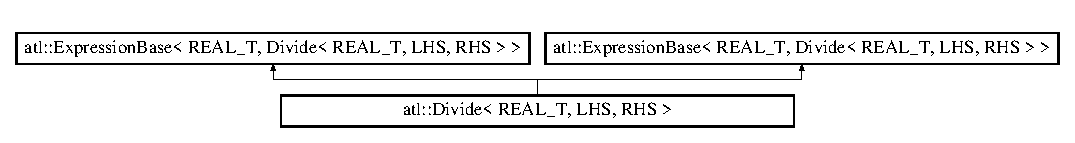
\includegraphics[height=1.469816cm]{structatl_1_1_divide}
\end{center}
\end{figure}
\subsection*{Public Types}
\begin{DoxyCompactItemize}
\item 
\hypertarget{structatl_1_1_divide_abf953ef2ef62117bc7c276e1764ce2cd}{typedef R\+E\+A\+L\+\_\+\+T {\bfseries B\+A\+S\+E\+\_\+\+T\+Y\+P\+E}}\label{structatl_1_1_divide_abf953ef2ef62117bc7c276e1764ce2cd}

\item 
\hypertarget{structatl_1_1_divide_abf953ef2ef62117bc7c276e1764ce2cd}{typedef R\+E\+A\+L\+\_\+\+T {\bfseries B\+A\+S\+E\+\_\+\+T\+Y\+P\+E}}\label{structatl_1_1_divide_abf953ef2ef62117bc7c276e1764ce2cd}

\end{DoxyCompactItemize}
\subsection*{Public Member Functions}
\begin{DoxyCompactItemize}
\item 
\hypertarget{structatl_1_1_divide_a6a73e9fdb3a745ac384b027797a51d64}{{\bfseries Divide} (const \hyperlink{structatl_1_1_expression_base}{Expression\+Base}$<$ R\+E\+A\+L\+\_\+\+T, L\+H\+S $>$ \&lhs, const \hyperlink{structatl_1_1_expression_base}{Expression\+Base}$<$ R\+E\+A\+L\+\_\+\+T, R\+H\+S $>$ \&rhs)}\label{structatl_1_1_divide_a6a73e9fdb3a745ac384b027797a51d64}

\item 
\hypertarget{structatl_1_1_divide_af1d32dc16af3a699e5bd5c386a4a9e7c}{{\bfseries Divide} (const R\+E\+A\+L\+\_\+\+T \&lhs, const \hyperlink{structatl_1_1_expression_base}{Expression\+Base}$<$ R\+E\+A\+L\+\_\+\+T, R\+H\+S $>$ \&rhs)}\label{structatl_1_1_divide_af1d32dc16af3a699e5bd5c386a4a9e7c}

\item 
\hypertarget{structatl_1_1_divide_ad9933af702709a62b3f4fb3fd238b0cb}{{\bfseries Divide} (const \hyperlink{structatl_1_1_expression_base}{Expression\+Base}$<$ R\+E\+A\+L\+\_\+\+T, L\+H\+S $>$ \&lhs, const R\+E\+A\+L\+\_\+\+T \&rhs)}\label{structatl_1_1_divide_ad9933af702709a62b3f4fb3fd238b0cb}

\item 
\hypertarget{structatl_1_1_divide_ae639697a3d873b9b027dc6ce6df195ad}{const R\+E\+A\+L\+\_\+\+T {\bfseries Get\+Value} () const }\label{structatl_1_1_divide_ae639697a3d873b9b027dc6ce6df195ad}

\item 
\hypertarget{structatl_1_1_divide_aee55c50583b536e4a6ef6e32b02d4054}{const R\+E\+A\+L\+\_\+\+T {\bfseries Get\+Value} (size\+\_\+t i, size\+\_\+t j=0) const }\label{structatl_1_1_divide_aee55c50583b536e4a6ef6e32b02d4054}

\item 
\hypertarget{structatl_1_1_divide_a1364bf196ce7e76665d8cb203786f3d8}{void {\bfseries Push\+Ids} (typename \hyperlink{structatl_1_1_stack_entry}{atl\+::\+Stack\+Entry}$<$ R\+E\+A\+L\+\_\+\+T $>$\+::vi\+\_\+storage \&ids) const }\label{structatl_1_1_divide_a1364bf196ce7e76665d8cb203786f3d8}

\item 
\hypertarget{structatl_1_1_divide_a43d0b1a7b9e721fac5388995d873b995}{void {\bfseries Push\+Ids} (typename \hyperlink{structatl_1_1_stack_entry}{atl\+::\+Stack\+Entry}$<$ R\+E\+A\+L\+\_\+\+T $>$\+::vi\+\_\+storage \&ids, size\+\_\+t i, size\+\_\+t j=0) const }\label{structatl_1_1_divide_a43d0b1a7b9e721fac5388995d873b995}

\item 
\hypertarget{structatl_1_1_divide_a0002c6a3821c0c667fb3bf8bfef08950}{const R\+E\+A\+L\+\_\+\+T {\bfseries Evaluate\+Derivative} (uint32\+\_\+t id) const }\label{structatl_1_1_divide_a0002c6a3821c0c667fb3bf8bfef08950}

\item 
\hypertarget{structatl_1_1_divide_ab1c0e0d04d00e8670f965bf50c86d92f}{R\+E\+A\+L\+\_\+\+T {\bfseries Evaluate\+Derivative} (uint32\+\_\+t a, uint32\+\_\+t b) const }\label{structatl_1_1_divide_ab1c0e0d04d00e8670f965bf50c86d92f}

\item 
\hypertarget{structatl_1_1_divide_a5cae35f64745a2e85da0f82383fa3b2e}{R\+E\+A\+L\+\_\+\+T {\bfseries Evaluate\+Derivative} (uint32\+\_\+t x, uint32\+\_\+t y, uint32\+\_\+t z) const }\label{structatl_1_1_divide_a5cae35f64745a2e85da0f82383fa3b2e}

\item 
\hypertarget{structatl_1_1_divide_a9bd2507a264c863e668927f4eba54dee}{R\+E\+A\+L\+\_\+\+T {\bfseries Evaluate\+Derivative} (uint32\+\_\+t a, size\+\_\+t i, size\+\_\+t j=0) const }\label{structatl_1_1_divide_a9bd2507a264c863e668927f4eba54dee}

\item 
\hypertarget{structatl_1_1_divide_ac07310b45c6aad8559519ced136beb86}{R\+E\+A\+L\+\_\+\+T {\bfseries Evaluate\+Derivative} (uint32\+\_\+t a, uint32\+\_\+t b, size\+\_\+t i, size\+\_\+t j=0) const }\label{structatl_1_1_divide_ac07310b45c6aad8559519ced136beb86}

\item 
\hypertarget{structatl_1_1_divide_aeffb1c9821da7e2332ae608dac5fed45}{R\+E\+A\+L\+\_\+\+T {\bfseries Evaluate\+Derivative} (uint32\+\_\+t x, uint32\+\_\+t y, uint32\+\_\+t z, size\+\_\+t i, size\+\_\+t j=0) const }\label{structatl_1_1_divide_aeffb1c9821da7e2332ae608dac5fed45}

\item 
\hypertarget{structatl_1_1_divide_ac0021998b955347f6f8adcab6027d271}{size\+\_\+t {\bfseries Get\+Columns} () const }\label{structatl_1_1_divide_ac0021998b955347f6f8adcab6027d271}

\item 
\hypertarget{structatl_1_1_divide_a8c2e57c4a7de5e95ced4953432e69ccf}{size\+\_\+t {\bfseries Get\+Rows} () const }\label{structatl_1_1_divide_a8c2e57c4a7de5e95ced4953432e69ccf}

\item 
\hypertarget{structatl_1_1_divide_a63953552caab4438cebcfee1a202e0f9}{bool {\bfseries Is\+Scalar} () const }\label{structatl_1_1_divide_a63953552caab4438cebcfee1a202e0f9}

\item 
\hyperlink{structatl_1_1_divide_a6a73e9fdb3a745ac384b027797a51d64}{Divide} (const \hyperlink{structatl_1_1_expression_base}{Expression\+Base}$<$ R\+E\+A\+L\+\_\+\+T, L\+H\+S $>$ \&lhs, const \hyperlink{structatl_1_1_expression_base}{Expression\+Base}$<$ R\+E\+A\+L\+\_\+\+T, R\+H\+S $>$ \&rhs)
\item 
\hyperlink{structatl_1_1_divide_af1d32dc16af3a699e5bd5c386a4a9e7c}{Divide} (const R\+E\+A\+L\+\_\+\+T \&lhs, const \hyperlink{structatl_1_1_expression_base}{Expression\+Base}$<$ R\+E\+A\+L\+\_\+\+T, R\+H\+S $>$ \&rhs)
\item 
\hyperlink{structatl_1_1_divide_ad9933af702709a62b3f4fb3fd238b0cb}{Divide} (const \hyperlink{structatl_1_1_expression_base}{Expression\+Base}$<$ R\+E\+A\+L\+\_\+\+T, L\+H\+S $>$ \&lhs, const R\+E\+A\+L\+\_\+\+T \&rhs)
\item 
const R\+E\+A\+L\+\_\+\+T \hyperlink{structatl_1_1_divide_ae639697a3d873b9b027dc6ce6df195ad}{Get\+Value} () const 
\item 
const R\+E\+A\+L\+\_\+\+T \hyperlink{structatl_1_1_divide_aee55c50583b536e4a6ef6e32b02d4054}{Get\+Value} (size\+\_\+t i, size\+\_\+t j=0) const 
\item 
bool \hyperlink{structatl_1_1_divide_acbea13449c17063d68f61f8afb45ce12}{Is\+Nonlinear} () const 
\item 
void \hyperlink{structatl_1_1_divide_a1364bf196ce7e76665d8cb203786f3d8}{Push\+Ids} (typename \hyperlink{structatl_1_1_stack_entry}{atl\+::\+Stack\+Entry}$<$ R\+E\+A\+L\+\_\+\+T $>$\+::vi\+\_\+storage \&ids) const 
\item 
void \hyperlink{structatl_1_1_divide_a43d0b1a7b9e721fac5388995d873b995}{Push\+Ids} (typename \hyperlink{structatl_1_1_stack_entry}{atl\+::\+Stack\+Entry}$<$ R\+E\+A\+L\+\_\+\+T $>$\+::vi\+\_\+storage \&ids, size\+\_\+t i, size\+\_\+t j=0) const 
\item 
const R\+E\+A\+L\+\_\+\+T \hyperlink{structatl_1_1_divide_a52c08dfa122348405f2122c161dc2883}{Evaluate\+Derivative} (uint32\+\_\+t x) const 
\item 
R\+E\+A\+L\+\_\+\+T \hyperlink{structatl_1_1_divide_aa7c1683046ed7b4f0a8dee864eff549c}{Evaluate\+Derivative} (uint32\+\_\+t x, uint32\+\_\+t y) const 
\item 
R\+E\+A\+L\+\_\+\+T \hyperlink{structatl_1_1_divide_a5cae35f64745a2e85da0f82383fa3b2e}{Evaluate\+Derivative} (uint32\+\_\+t x, uint32\+\_\+t y, uint32\+\_\+t z) const 
\item 
R\+E\+A\+L\+\_\+\+T \hyperlink{structatl_1_1_divide_ad4ac0ce5afaf2098e6c2fe70aca0b9c9}{Evaluate\+Derivative} (uint32\+\_\+t x, size\+\_\+t i, size\+\_\+t j=0) const 
\item 
R\+E\+A\+L\+\_\+\+T \hyperlink{structatl_1_1_divide_aa6fdd0114a0fa75e08d772dfba2e6c08}{Evaluate\+Derivative} (uint32\+\_\+t x, uint32\+\_\+t y, size\+\_\+t i, size\+\_\+t j=0) const 
\item 
R\+E\+A\+L\+\_\+\+T \hyperlink{structatl_1_1_divide_aeffb1c9821da7e2332ae608dac5fed45}{Evaluate\+Derivative} (uint32\+\_\+t x, uint32\+\_\+t y, uint32\+\_\+t z, size\+\_\+t i, size\+\_\+t j=0) const 
\item 
size\+\_\+t \hyperlink{structatl_1_1_divide_ac0021998b955347f6f8adcab6027d271}{Get\+Columns} () const 
\item 
size\+\_\+t \hyperlink{structatl_1_1_divide_a8c2e57c4a7de5e95ced4953432e69ccf}{Get\+Rows} () const 
\item 
bool \hyperlink{structatl_1_1_divide_a63953552caab4438cebcfee1a202e0f9}{Is\+Scalar} () const 
\item 
const std\+::string \hyperlink{structatl_1_1_divide_acf032259c4e257e00a929d9cd33f6901}{To\+Expression\+Template\+String} () const 
\end{DoxyCompactItemize}
\subsection*{Public Attributes}
\begin{DoxyCompactItemize}
\item 
\hypertarget{structatl_1_1_divide_a3318f15b1e95a5ff1ababd48cb3e57fd}{\hyperlink{structatl_1_1_real}{atl\+::\+Real}$<$ R\+E\+A\+L\+\_\+\+T $>$ {\bfseries real\+\_\+m}}\label{structatl_1_1_divide_a3318f15b1e95a5ff1ababd48cb3e57fd}

\item 
\hypertarget{structatl_1_1_divide_ac7126091b9651fdb2e8e7486226de9bb}{const L\+H\+S \& {\bfseries lhs\+\_\+m}}\label{structatl_1_1_divide_ac7126091b9651fdb2e8e7486226de9bb}

\item 
\hypertarget{structatl_1_1_divide_abf3fccd9c87ab543801eefc34dbadda0}{const R\+H\+S \& {\bfseries rhs\+\_\+m}}\label{structatl_1_1_divide_abf3fccd9c87ab543801eefc34dbadda0}

\item 
\hypertarget{structatl_1_1_divide_a6fb97b4a014be1e21a2fbcedcc74697a}{R\+E\+A\+L\+\_\+\+T {\bfseries value\+\_\+m}}\label{structatl_1_1_divide_a6fb97b4a014be1e21a2fbcedcc74697a}

\end{DoxyCompactItemize}


\subsection{Detailed Description}
\subsubsection*{template$<$class R\+E\+A\+L\+\_\+\+T, class L\+H\+S, class R\+H\+S$>$struct atl\+::\+Divide$<$ R\+E\+A\+L\+\_\+\+T, L\+H\+S, R\+H\+S $>$}

Expression template to handle

$ f(x) / g(x) $

or

$ f_{i,j}(x) / g_{i,j}(x) $ 

\subsection{Constructor \& Destructor Documentation}
\hypertarget{structatl_1_1_divide_a6a73e9fdb3a745ac384b027797a51d64}{\index{atl\+::\+Divide@{atl\+::\+Divide}!Divide@{Divide}}
\index{Divide@{Divide}!atl\+::\+Divide@{atl\+::\+Divide}}
\subsubsection[{Divide}]{\setlength{\rightskip}{0pt plus 5cm}template$<$class R\+E\+A\+L\+\_\+\+T , class L\+H\+S , class R\+H\+S $>$ {\bf atl\+::\+Divide}$<$ R\+E\+A\+L\+\_\+\+T, L\+H\+S, R\+H\+S $>$\+::{\bf Divide} (
\begin{DoxyParamCaption}
\item[{const {\bf Expression\+Base}$<$ R\+E\+A\+L\+\_\+\+T, L\+H\+S $>$ \&}]{lhs, }
\item[{const {\bf Expression\+Base}$<$ R\+E\+A\+L\+\_\+\+T, R\+H\+S $>$ \&}]{rhs}
\end{DoxyParamCaption}
)\hspace{0.3cm}{\ttfamily [inline]}}}\label{structatl_1_1_divide_a6a73e9fdb3a745ac384b027797a51d64}
Constructor for two variable types.


\begin{DoxyParams}{Parameters}
{\em lhs} & \\
\hline
{\em rhs} & \\
\hline
\end{DoxyParams}
\hypertarget{structatl_1_1_divide_af1d32dc16af3a699e5bd5c386a4a9e7c}{\index{atl\+::\+Divide@{atl\+::\+Divide}!Divide@{Divide}}
\index{Divide@{Divide}!atl\+::\+Divide@{atl\+::\+Divide}}
\subsubsection[{Divide}]{\setlength{\rightskip}{0pt plus 5cm}template$<$class R\+E\+A\+L\+\_\+\+T , class L\+H\+S , class R\+H\+S $>$ {\bf atl\+::\+Divide}$<$ R\+E\+A\+L\+\_\+\+T, L\+H\+S, R\+H\+S $>$\+::{\bf Divide} (
\begin{DoxyParamCaption}
\item[{const R\+E\+A\+L\+\_\+\+T \&}]{lhs, }
\item[{const {\bf Expression\+Base}$<$ R\+E\+A\+L\+\_\+\+T, R\+H\+S $>$ \&}]{rhs}
\end{DoxyParamCaption}
)\hspace{0.3cm}{\ttfamily [inline]}}}\label{structatl_1_1_divide_af1d32dc16af3a699e5bd5c386a4a9e7c}
Constructor for a real divided by a variable type.


\begin{DoxyParams}{Parameters}
{\em lhs} & \\
\hline
{\em rhs} & \\
\hline
\end{DoxyParams}
\hypertarget{structatl_1_1_divide_ad9933af702709a62b3f4fb3fd238b0cb}{\index{atl\+::\+Divide@{atl\+::\+Divide}!Divide@{Divide}}
\index{Divide@{Divide}!atl\+::\+Divide@{atl\+::\+Divide}}
\subsubsection[{Divide}]{\setlength{\rightskip}{0pt plus 5cm}template$<$class R\+E\+A\+L\+\_\+\+T , class L\+H\+S , class R\+H\+S $>$ {\bf atl\+::\+Divide}$<$ R\+E\+A\+L\+\_\+\+T, L\+H\+S, R\+H\+S $>$\+::{\bf Divide} (
\begin{DoxyParamCaption}
\item[{const {\bf Expression\+Base}$<$ R\+E\+A\+L\+\_\+\+T, L\+H\+S $>$ \&}]{lhs, }
\item[{const R\+E\+A\+L\+\_\+\+T \&}]{rhs}
\end{DoxyParamCaption}
)\hspace{0.3cm}{\ttfamily [inline]}}}\label{structatl_1_1_divide_ad9933af702709a62b3f4fb3fd238b0cb}
Constructor for a variable divided by a real type.


\begin{DoxyParams}{Parameters}
{\em lhs} & \\
\hline
{\em rhs} & \\
\hline
\end{DoxyParams}


\subsection{Member Function Documentation}
\hypertarget{structatl_1_1_divide_a52c08dfa122348405f2122c161dc2883}{\index{atl\+::\+Divide@{atl\+::\+Divide}!Evaluate\+Derivative@{Evaluate\+Derivative}}
\index{Evaluate\+Derivative@{Evaluate\+Derivative}!atl\+::\+Divide@{atl\+::\+Divide}}
\subsubsection[{Evaluate\+Derivative}]{\setlength{\rightskip}{0pt plus 5cm}template$<$class R\+E\+A\+L\+\_\+\+T , class L\+H\+S , class R\+H\+S $>$ const R\+E\+A\+L\+\_\+\+T {\bf atl\+::\+Divide}$<$ R\+E\+A\+L\+\_\+\+T, L\+H\+S, R\+H\+S $>$\+::Evaluate\+Derivative (
\begin{DoxyParamCaption}
\item[{uint32\+\_\+t}]{x}
\end{DoxyParamCaption}
) const\hspace{0.3cm}{\ttfamily [inline]}}}\label{structatl_1_1_divide_a52c08dfa122348405f2122c161dc2883}
Evaluates the first-\/order derivative with respect to x.

$ {{{{d}\over{d\,x}}\,f(x)}\over{g(x)}}-{{f(x)\, \left({{d}\over{d\,x}}\,g(x)\right)}\over{g(x)^2}} $


\begin{DoxyParams}{Parameters}
{\em x} & \\
\hline
\end{DoxyParams}
\begin{DoxyReturn}{Returns}

\end{DoxyReturn}
\hypertarget{structatl_1_1_divide_aa7c1683046ed7b4f0a8dee864eff549c}{\index{atl\+::\+Divide@{atl\+::\+Divide}!Evaluate\+Derivative@{Evaluate\+Derivative}}
\index{Evaluate\+Derivative@{Evaluate\+Derivative}!atl\+::\+Divide@{atl\+::\+Divide}}
\subsubsection[{Evaluate\+Derivative}]{\setlength{\rightskip}{0pt plus 5cm}template$<$class R\+E\+A\+L\+\_\+\+T , class L\+H\+S , class R\+H\+S $>$ R\+E\+A\+L\+\_\+\+T {\bf atl\+::\+Divide}$<$ R\+E\+A\+L\+\_\+\+T, L\+H\+S, R\+H\+S $>$\+::Evaluate\+Derivative (
\begin{DoxyParamCaption}
\item[{uint32\+\_\+t}]{x, }
\item[{uint32\+\_\+t}]{y}
\end{DoxyParamCaption}
) const\hspace{0.3cm}{\ttfamily [inline]}}}\label{structatl_1_1_divide_aa7c1683046ed7b4f0a8dee864eff549c}
Evaluates the second-\/order derivative with respect to x and y.

$ {{2\,f(x,y)\,\left({{d}\over{d\,x}}\,g(x,y)\right)\, \left({{d}\over{d\,y}}\,g(x,y)\right)}\over{g(x,y)^3}}- {{{{d}\over{d\,x}}\,f(x,y)\,\left({{d}\over{d\,y}}\,g(x, y)\right)}\over{g(x,y)^2}}- \\ {{f(x,y)\,\left({{d^2}\over{d \,x\,d\,y}}\,g(x,y)\right)}\over{g(x,y)^2}}-{{{{d}\over{ d\,y}}\,f(x,y)\,\left({{d}\over{d\,x}}\,g(x,y)\right) }\over{g(x,y)^2}}+{{{{d^2}\over{d\,x\,d\,y}}\,f(x,y) }\over{g(x,y)}} $


\begin{DoxyParams}{Parameters}
{\em x} & \\
\hline
{\em y} & \\
\hline
\end{DoxyParams}
\begin{DoxyReturn}{Returns}

\end{DoxyReturn}
\hypertarget{structatl_1_1_divide_a5cae35f64745a2e85da0f82383fa3b2e}{\index{atl\+::\+Divide@{atl\+::\+Divide}!Evaluate\+Derivative@{Evaluate\+Derivative}}
\index{Evaluate\+Derivative@{Evaluate\+Derivative}!atl\+::\+Divide@{atl\+::\+Divide}}
\subsubsection[{Evaluate\+Derivative}]{\setlength{\rightskip}{0pt plus 5cm}template$<$class R\+E\+A\+L\+\_\+\+T , class L\+H\+S , class R\+H\+S $>$ R\+E\+A\+L\+\_\+\+T {\bf atl\+::\+Divide}$<$ R\+E\+A\+L\+\_\+\+T, L\+H\+S, R\+H\+S $>$\+::Evaluate\+Derivative (
\begin{DoxyParamCaption}
\item[{uint32\+\_\+t}]{x, }
\item[{uint32\+\_\+t}]{y, }
\item[{uint32\+\_\+t}]{z}
\end{DoxyParamCaption}
) const\hspace{0.3cm}{\ttfamily [inline]}}}\label{structatl_1_1_divide_a5cae35f64745a2e85da0f82383fa3b2e}
Evaluates the third-\/order derivative with respect to x, y, and z.

$ -{{6\,f\left(x , y , z\right)\,\left({{d}\over{d\,x}}\,g\left(x , y , z\right)\right)\,\left({{d}\over{d\,y}}\,g\left(x , y , z\right) \right)\,\left({{d}\over{d\,z}}\,g\left(x , y , z\right)\right) }\over{g^4\left(x , y , z\right)}}+{{2\,\left({{d}\over{d\,x}}\,f \left(x , y , z\right)\right)\,\left({{d}\over{d\,y}}\,g\left(x , y , z\right)\right)\,\left({{d}\over{d\,z}}\,g\left(x , y , z\right) \right)}\over{g^3\left(x , y , z\right)}}+{{2\,f\left(x , y , z \right)\,\left({{d^2}\over{d\,x\,d\,y}}\,g\left(x , y , z\right) \right)\,\left({{d}\over{d\,z}}\,g\left(x , y , z\right)\right) }\over{g^3\left(x , y , z\right)}}+ \\ {{2\,\left({{d}\over{d\,y}}\,f \left(x , y , z\right)\right)\,\left({{d}\over{d\,x}}\,g\left(x , y , z\right)\right)\,\left({{d}\over{d\,z}}\,g\left(x , y , z\right) \right)}\over{g^3\left(x , y , z\right)}}-{{{{d^2}\over{d\,x\,d\,y}} \,f\left(x , y , z\right)\,\left({{d}\over{d\,z}}\,g\left(x , y , z \right)\right)}\over{g^2\left(x , y , z\right)}}+{{2\,f\left(x , y , z\right)\,\left({{d}\over{d\,x}}\,g\left(x , y , z\right)\right) \,\left({{d^2}\over{d\,y\,d\,z}}\,g\left(x , y , z\right)\right) }\over{g^3\left(x , y , z\right)}}-{{{{d}\over{d\,x}}\,f\left(x , y , z\right)\,\left({{d^2}\over{d\,y\,d\,z}}\,g\left(x , y , z\right) \right)}\over{g^2\left(x , y , z\right)}}+{{2\,f\left(x , y , z \right)\,\left({{d^2}\over{d\,x\,d\,z}}\,g\left(x , y , z\right) \right)\,\left({{d}\over{d\,y}}\,g\left(x , y , z\right)\right) }\over{g^3\left(x , y , z\right)}}+ \\ {{2\,\left({{d}\over{d\,z}}\,f \left(x , y , z\right)\right)\,\left({{d}\over{d\,x}}\,g\left(x , y , z\right)\right)\,\left({{d}\over{d\,y}}\,g\left(x , y , z\right) \right)}\over{g^3\left(x , y , z\right)}}-{{{{d^2}\over{d\,x\,d\,z}} \,f\left(x , y , z\right)\,\left({{d}\over{d\,y}}\,g\left(x , y , z \right)\right)}\over{g^2\left(x , y , z\right)}}-{{{{d}\over{d\,y}} \,f\left(x , y , z\right)\,\left({{d^2}\over{d\,x\,d\,z}}\,g\left(x , y , z\right)\right)}\over{g^2\left(x , y , z\right)}}-{{f\left(x , y , z\right)\,\left({{d^3}\over{d\,x\,d\,y\,d\,z}}\,g\left(x , y , z\right)\right)}\over{g^2\left(x , y , z\right)}}-{{{{d}\over{d\, z}}\,f\left(x , y , z\right)\,\left({{d^2}\over{d\,x\,d\,y}}\,g \left(x , y , z\right)\right)}\over{g^2\left(x , y , z\right)}}-{{{{ d^2}\over{d\,y\,d\,z}}\,f\left(x , y , z\right)\,\left({{d}\over{d\, x}}\,g\left(x , y , z\right)\right)}\over{g^2\left(x , y , z\right) }}+{{{{d^3}\over{d\,x\,d\,y\,d\,z}}\,f\left(x , y , z\right)}\over{g \left(x , y , z\right)}} $


\begin{DoxyParams}{Parameters}
{\em x} & \\
\hline
{\em y} & \\
\hline
{\em z} & \\
\hline
\end{DoxyParams}
\begin{DoxyReturn}{Returns}

\end{DoxyReturn}
\hypertarget{structatl_1_1_divide_ad4ac0ce5afaf2098e6c2fe70aca0b9c9}{\index{atl\+::\+Divide@{atl\+::\+Divide}!Evaluate\+Derivative@{Evaluate\+Derivative}}
\index{Evaluate\+Derivative@{Evaluate\+Derivative}!atl\+::\+Divide@{atl\+::\+Divide}}
\subsubsection[{Evaluate\+Derivative}]{\setlength{\rightskip}{0pt plus 5cm}template$<$class R\+E\+A\+L\+\_\+\+T , class L\+H\+S , class R\+H\+S $>$ R\+E\+A\+L\+\_\+\+T {\bf atl\+::\+Divide}$<$ R\+E\+A\+L\+\_\+\+T, L\+H\+S, R\+H\+S $>$\+::Evaluate\+Derivative (
\begin{DoxyParamCaption}
\item[{uint32\+\_\+t}]{x, }
\item[{size\+\_\+t}]{i, }
\item[{size\+\_\+t}]{j = {\ttfamily 0}}
\end{DoxyParamCaption}
) const\hspace{0.3cm}{\ttfamily [inline]}}}\label{structatl_1_1_divide_ad4ac0ce5afaf2098e6c2fe70aca0b9c9}
Evaluates the first-\/order derivative with respect to x.

$ {{{{d}\over{d\,x}}\,f_{i,j}(x)}\over{g_{i,j}(x)}}-{{f_{i,j}(x)\, \left({{d}\over{d\,x}}\,g_{i,j}(x)\right)}\over{g_{i,j}(x)^2}} $


\begin{DoxyParams}{Parameters}
{\em x} & \\
\hline
\end{DoxyParams}
\begin{DoxyReturn}{Returns}

\end{DoxyReturn}
\hypertarget{structatl_1_1_divide_aa6fdd0114a0fa75e08d772dfba2e6c08}{\index{atl\+::\+Divide@{atl\+::\+Divide}!Evaluate\+Derivative@{Evaluate\+Derivative}}
\index{Evaluate\+Derivative@{Evaluate\+Derivative}!atl\+::\+Divide@{atl\+::\+Divide}}
\subsubsection[{Evaluate\+Derivative}]{\setlength{\rightskip}{0pt plus 5cm}template$<$class R\+E\+A\+L\+\_\+\+T , class L\+H\+S , class R\+H\+S $>$ R\+E\+A\+L\+\_\+\+T {\bf atl\+::\+Divide}$<$ R\+E\+A\+L\+\_\+\+T, L\+H\+S, R\+H\+S $>$\+::Evaluate\+Derivative (
\begin{DoxyParamCaption}
\item[{uint32\+\_\+t}]{x, }
\item[{uint32\+\_\+t}]{y, }
\item[{size\+\_\+t}]{i, }
\item[{size\+\_\+t}]{j = {\ttfamily 0}}
\end{DoxyParamCaption}
) const\hspace{0.3cm}{\ttfamily [inline]}}}\label{structatl_1_1_divide_aa6fdd0114a0fa75e08d772dfba2e6c08}
Evaluates the second-\/order derivative with respect to x and y at index \{i,j\}.

$ {{2\,f_{i,j}(x,y)\,\left({{d}\over{d\,x}}\,g_{i,j}(x,y)\right)\, \left({{d}\over{d\,y}}\,g_{i,j}(x,y)\right)}\over{g_{i,j}(x,y)^3}}- {{{{d}\over{d\,x}}\,f_{i,j}(x,y)\,\left({{d}\over{d\,y}}\,g_{i,j}(x, y)\right)}\over{g_{i,j}(x,y)^2}}- \\ {{f_{i,j}(x,y)\,\left({{d^2}\over{d \,x\,d\,y}}\,g_{i,j}(x,y)\right)}\over{g_{i,j}(x,y)^2}}-{{{{d}\over{ d\,y}}\,f_{i,j}(x,y)\,\left({{d}\over{d\,x}}\,g_{i,j}(x,y)\right) }\over{g_{i,j}(x,y)^2}}+{{{{d^2}\over{d\,x\,d\,y}}\,f_{i,j}(x,y) }\over{g_{i,j}(x,y)}} $


\begin{DoxyParams}{Parameters}
{\em x} & \\
\hline
{\em y} & \\
\hline
{\em i} & \\
\hline
{\em j} & \\
\hline
\end{DoxyParams}
\begin{DoxyReturn}{Returns}

\end{DoxyReturn}
\hypertarget{structatl_1_1_divide_aeffb1c9821da7e2332ae608dac5fed45}{\index{atl\+::\+Divide@{atl\+::\+Divide}!Evaluate\+Derivative@{Evaluate\+Derivative}}
\index{Evaluate\+Derivative@{Evaluate\+Derivative}!atl\+::\+Divide@{atl\+::\+Divide}}
\subsubsection[{Evaluate\+Derivative}]{\setlength{\rightskip}{0pt plus 5cm}template$<$class R\+E\+A\+L\+\_\+\+T , class L\+H\+S , class R\+H\+S $>$ R\+E\+A\+L\+\_\+\+T {\bf atl\+::\+Divide}$<$ R\+E\+A\+L\+\_\+\+T, L\+H\+S, R\+H\+S $>$\+::Evaluate\+Derivative (
\begin{DoxyParamCaption}
\item[{uint32\+\_\+t}]{x, }
\item[{uint32\+\_\+t}]{y, }
\item[{uint32\+\_\+t}]{z, }
\item[{size\+\_\+t}]{i, }
\item[{size\+\_\+t}]{j = {\ttfamily 0}}
\end{DoxyParamCaption}
) const\hspace{0.3cm}{\ttfamily [inline]}}}\label{structatl_1_1_divide_aeffb1c9821da7e2332ae608dac5fed45}
Evaluates the third-\/order derivative with respect to x, y, and z at index \{i,j\}.

$ -{{6\,f_{i,j}(x,y,z)\,\left({{d}\over{d\,x}}\,g_{i,j}(x,y,z)\right) \,\left({{d}\over{d\,y}}\,g_{i,j}(x,y,z)\right)\,\left({{d}\over{d\, z}}\,g_{i,j}(x,y,z)\right)}\over{g_{i,j}(x,y,z)^4}}+{{2\,\left({{d }\over{d\,x}}\,f_{i,j}(x,y,z)\right)\,\left({{d}\over{d\,y}}\,g_{i,j }(x,y,z)\right)\,\left({{d}\over{d\,z}}\,g_{i,j}(x,y,z)\right) }\over{g_{i,j}(x,y,z)^3}}+{{2\,f_{i,j}(x,y,z)\,\left({{d^2}\over{d\, x\,d\,y}}\,g_{i,j}(x,y,z)\right)\,\left({{d}\over{d\,z}}\,g_{i,j}(x, y,z)\right)}\over{g_{i,j}(x,y,z)^3}}+ \\ {{2\,\left({{d}\over{d\,y}}\,f _{i,j}(x,y,z)\right)\,\left({{d}\over{d\,x}}\,g_{i,j}(x,y,z)\right) \,\left({{d}\over{d\,z}}\,g_{i,j}(x,y,z)\right)}\over{g_{i,j}(x,y,z) ^3}}-{{{{d^2}\over{d\,x\,d\,y}}\,f_{i,j}(x,y,z)\,\left({{d}\over{d\, z}}\,g_{i,j}(x,y,z)\right)}\over{g_{i,j}(x,y,z)^2}}+{{2\,f_{i,j}(x,y ,z)\,\left({{d}\over{d\,x}}\,g_{i,j}(x,y,z)\right)\,\left({{d^2 }\over{d\,y\,d\,z}}\,g_{i,j}(x,y,z)\right)}\over{g_{i,j}(x,y,z)^3}}- {{{{d}\over{d\,x}}\,f_{i,j}(x,y,z)\,\left({{d^2}\over{d\,y\,d\,z}}\, g_{i,j}(x,y,z)\right)}\over{g_{i,j}(x,y,z)^2}}+ \\ {{2\,f_{i,j}(x,y,z)\, \left({{d^2}\over{d\,x\,d\,z}}\,g_{i,j}(x,y,z)\right)\,\left({{d }\over{d\,y}}\,g_{i,j}(x,y,z)\right)}\over{g_{i,j}(x,y,z)^3}}+{{2\, \left({{d}\over{d\,z}}\,f_{i,j}(x,y,z)\right)\,\left({{d}\over{d\,x }}\,g_{i,j}(x,y,z)\right)\,\left({{d}\over{d\,y}}\,g_{i,j}(x,y,z) \right)}\over{g_{i,j}(x,y,z)^3}}-{{{{d^2}\over{d\,x\,d\,z}}\,f_{i,j} (x,y,z)\,\left({{d}\over{d\,y}}\,g_{i,j}(x,y,z)\right)}\over{g_{i,j} (x,y,z)^2}}-{{{{d}\over{d\,y}}\,f_{i,j}(x,y,z)\,\left({{d^2}\over{d \,x\,d\,z}}\,g_{i,j}(x,y,z)\right)}\over{g_{i,j}(x,y,z)^2}}-{{f_{i,j }(x,y,z)\,\left({{d^3}\over{d\,x\,d\,y\,d\,z}}\,g_{i,j}(x,y,z) \right)}\over{g_{i,j}(x,y,z)^2}}- \\ {{{{d}\over{d\,z}}\,f_{i,j}(x,y,z) \,\left({{d^2}\over{d\,x\,d\,y}}\,g_{i,j}(x,y,z)\right)}\over{g_{i,j }(x,y,z)^2}}-{{{{d^2}\over{d\,y\,d\,z}}\,f_{i,j}(x,y,z)\,\left({{d }\over{d\,x}}\,g_{i,j}(x,y,z)\right)}\over{g_{i,j}(x,y,z)^2}}+{{{{d^ 3}\over{d\,x\,d\,y\,d\,z}}\,f_{i,j}(x,y,z)}\over{g_{i,j}(x,y,z)}} $


\begin{DoxyParams}{Parameters}
{\em x} & \\
\hline
{\em y} & \\
\hline
{\em z} & \\
\hline
{\em i} & \\
\hline
{\em j} & \\
\hline
\end{DoxyParams}
\begin{DoxyReturn}{Returns}

\end{DoxyReturn}
\hypertarget{structatl_1_1_divide_ac0021998b955347f6f8adcab6027d271}{\index{atl\+::\+Divide@{atl\+::\+Divide}!Get\+Columns@{Get\+Columns}}
\index{Get\+Columns@{Get\+Columns}!atl\+::\+Divide@{atl\+::\+Divide}}
\subsubsection[{Get\+Columns}]{\setlength{\rightskip}{0pt plus 5cm}template$<$class R\+E\+A\+L\+\_\+\+T , class L\+H\+S , class R\+H\+S $>$ size\+\_\+t {\bf atl\+::\+Divide}$<$ R\+E\+A\+L\+\_\+\+T, L\+H\+S, R\+H\+S $>$\+::Get\+Columns (
\begin{DoxyParamCaption}
{}
\end{DoxyParamCaption}
) const\hspace{0.3cm}{\ttfamily [inline]}}}\label{structatl_1_1_divide_ac0021998b955347f6f8adcab6027d271}
Return the number of columns.

\begin{DoxyReturn}{Returns}

\end{DoxyReturn}
\hypertarget{structatl_1_1_divide_a8c2e57c4a7de5e95ced4953432e69ccf}{\index{atl\+::\+Divide@{atl\+::\+Divide}!Get\+Rows@{Get\+Rows}}
\index{Get\+Rows@{Get\+Rows}!atl\+::\+Divide@{atl\+::\+Divide}}
\subsubsection[{Get\+Rows}]{\setlength{\rightskip}{0pt plus 5cm}template$<$class R\+E\+A\+L\+\_\+\+T , class L\+H\+S , class R\+H\+S $>$ size\+\_\+t {\bf atl\+::\+Divide}$<$ R\+E\+A\+L\+\_\+\+T, L\+H\+S, R\+H\+S $>$\+::Get\+Rows (
\begin{DoxyParamCaption}
{}
\end{DoxyParamCaption}
) const\hspace{0.3cm}{\ttfamily [inline]}}}\label{structatl_1_1_divide_a8c2e57c4a7de5e95ced4953432e69ccf}
Return the number of rows.

\begin{DoxyReturn}{Returns}

\end{DoxyReturn}
\hypertarget{structatl_1_1_divide_ae639697a3d873b9b027dc6ce6df195ad}{\index{atl\+::\+Divide@{atl\+::\+Divide}!Get\+Value@{Get\+Value}}
\index{Get\+Value@{Get\+Value}!atl\+::\+Divide@{atl\+::\+Divide}}
\subsubsection[{Get\+Value}]{\setlength{\rightskip}{0pt plus 5cm}template$<$class R\+E\+A\+L\+\_\+\+T , class L\+H\+S , class R\+H\+S $>$ const R\+E\+A\+L\+\_\+\+T {\bf atl\+::\+Divide}$<$ R\+E\+A\+L\+\_\+\+T, L\+H\+S, R\+H\+S $>$\+::Get\+Value (
\begin{DoxyParamCaption}
{}
\end{DoxyParamCaption}
) const\hspace{0.3cm}{\ttfamily [inline]}}}\label{structatl_1_1_divide_ae639697a3d873b9b027dc6ce6df195ad}
Compute the division of lhs by rhs.

\begin{DoxyReturn}{Returns}

\end{DoxyReturn}
\hypertarget{structatl_1_1_divide_aee55c50583b536e4a6ef6e32b02d4054}{\index{atl\+::\+Divide@{atl\+::\+Divide}!Get\+Value@{Get\+Value}}
\index{Get\+Value@{Get\+Value}!atl\+::\+Divide@{atl\+::\+Divide}}
\subsubsection[{Get\+Value}]{\setlength{\rightskip}{0pt plus 5cm}template$<$class R\+E\+A\+L\+\_\+\+T , class L\+H\+S , class R\+H\+S $>$ const R\+E\+A\+L\+\_\+\+T {\bf atl\+::\+Divide}$<$ R\+E\+A\+L\+\_\+\+T, L\+H\+S, R\+H\+S $>$\+::Get\+Value (
\begin{DoxyParamCaption}
\item[{size\+\_\+t}]{i, }
\item[{size\+\_\+t}]{j = {\ttfamily 0}}
\end{DoxyParamCaption}
) const\hspace{0.3cm}{\ttfamily [inline]}}}\label{structatl_1_1_divide_aee55c50583b536e4a6ef6e32b02d4054}
Compute the division of the lhs and rhs expressions at index \{i,j\}.

\begin{DoxyReturn}{Returns}

\end{DoxyReturn}
\hypertarget{structatl_1_1_divide_acbea13449c17063d68f61f8afb45ce12}{\index{atl\+::\+Divide@{atl\+::\+Divide}!Is\+Nonlinear@{Is\+Nonlinear}}
\index{Is\+Nonlinear@{Is\+Nonlinear}!atl\+::\+Divide@{atl\+::\+Divide}}
\subsubsection[{Is\+Nonlinear}]{\setlength{\rightskip}{0pt plus 5cm}template$<$class R\+E\+A\+L\+\_\+\+T , class L\+H\+S , class R\+H\+S $>$ bool {\bf atl\+::\+Divide}$<$ R\+E\+A\+L\+\_\+\+T, L\+H\+S, R\+H\+S $>$\+::Is\+Nonlinear (
\begin{DoxyParamCaption}
{}
\end{DoxyParamCaption}
) const\hspace{0.3cm}{\ttfamily [inline]}}}\label{structatl_1_1_divide_acbea13449c17063d68f61f8afb45ce12}
Returns true if the left or right side is nonlinear, else false. \begin{DoxyReturn}{Returns}

\end{DoxyReturn}
\hypertarget{structatl_1_1_divide_a63953552caab4438cebcfee1a202e0f9}{\index{atl\+::\+Divide@{atl\+::\+Divide}!Is\+Scalar@{Is\+Scalar}}
\index{Is\+Scalar@{Is\+Scalar}!atl\+::\+Divide@{atl\+::\+Divide}}
\subsubsection[{Is\+Scalar}]{\setlength{\rightskip}{0pt plus 5cm}template$<$class R\+E\+A\+L\+\_\+\+T , class L\+H\+S , class R\+H\+S $>$ bool {\bf atl\+::\+Divide}$<$ R\+E\+A\+L\+\_\+\+T, L\+H\+S, R\+H\+S $>$\+::Is\+Scalar (
\begin{DoxyParamCaption}
{}
\end{DoxyParamCaption}
) const\hspace{0.3cm}{\ttfamily [inline]}}}\label{structatl_1_1_divide_a63953552caab4438cebcfee1a202e0f9}
True if the expression is a scalar. \begin{DoxyReturn}{Returns}

\end{DoxyReturn}
\hypertarget{structatl_1_1_divide_a1364bf196ce7e76665d8cb203786f3d8}{\index{atl\+::\+Divide@{atl\+::\+Divide}!Push\+Ids@{Push\+Ids}}
\index{Push\+Ids@{Push\+Ids}!atl\+::\+Divide@{atl\+::\+Divide}}
\subsubsection[{Push\+Ids}]{\setlength{\rightskip}{0pt plus 5cm}template$<$class R\+E\+A\+L\+\_\+\+T , class L\+H\+S , class R\+H\+S $>$ void {\bf atl\+::\+Divide}$<$ R\+E\+A\+L\+\_\+\+T, L\+H\+S, R\+H\+S $>$\+::Push\+Ids (
\begin{DoxyParamCaption}
\item[{typename {\bf atl\+::\+Stack\+Entry}$<$ R\+E\+A\+L\+\_\+\+T $>$\+::vi\+\_\+storage \&}]{ids}
\end{DoxyParamCaption}
) const\hspace{0.3cm}{\ttfamily [inline]}}}\label{structatl_1_1_divide_a1364bf196ce7e76665d8cb203786f3d8}
Push variable info into a set.


\begin{DoxyParams}{Parameters}
{\em ids} & \\
\hline
\end{DoxyParams}
\hypertarget{structatl_1_1_divide_a43d0b1a7b9e721fac5388995d873b995}{\index{atl\+::\+Divide@{atl\+::\+Divide}!Push\+Ids@{Push\+Ids}}
\index{Push\+Ids@{Push\+Ids}!atl\+::\+Divide@{atl\+::\+Divide}}
\subsubsection[{Push\+Ids}]{\setlength{\rightskip}{0pt plus 5cm}template$<$class R\+E\+A\+L\+\_\+\+T , class L\+H\+S , class R\+H\+S $>$ void {\bf atl\+::\+Divide}$<$ R\+E\+A\+L\+\_\+\+T, L\+H\+S, R\+H\+S $>$\+::Push\+Ids (
\begin{DoxyParamCaption}
\item[{typename {\bf atl\+::\+Stack\+Entry}$<$ R\+E\+A\+L\+\_\+\+T $>$\+::vi\+\_\+storage \&}]{ids, }
\item[{size\+\_\+t}]{i, }
\item[{size\+\_\+t}]{j = {\ttfamily 0}}
\end{DoxyParamCaption}
) const\hspace{0.3cm}{\ttfamily [inline]}}}\label{structatl_1_1_divide_a43d0b1a7b9e721fac5388995d873b995}
Push variable info into a set at index \{i,j\}.


\begin{DoxyParams}{Parameters}
{\em ids} & \\
\hline
{\em i} & \\
\hline
{\em j} & \\
\hline
\end{DoxyParams}
\hypertarget{structatl_1_1_divide_acf032259c4e257e00a929d9cd33f6901}{\index{atl\+::\+Divide@{atl\+::\+Divide}!To\+Expression\+Template\+String@{To\+Expression\+Template\+String}}
\index{To\+Expression\+Template\+String@{To\+Expression\+Template\+String}!atl\+::\+Divide@{atl\+::\+Divide}}
\subsubsection[{To\+Expression\+Template\+String}]{\setlength{\rightskip}{0pt plus 5cm}template$<$class R\+E\+A\+L\+\_\+\+T , class L\+H\+S , class R\+H\+S $>$ const std\+::string {\bf atl\+::\+Divide}$<$ R\+E\+A\+L\+\_\+\+T, L\+H\+S, R\+H\+S $>$\+::To\+Expression\+Template\+String (
\begin{DoxyParamCaption}
{}
\end{DoxyParamCaption}
) const\hspace{0.3cm}{\ttfamily [inline]}}}\label{structatl_1_1_divide_acf032259c4e257e00a929d9cd33f6901}
Create a string representation of this expression template.

\begin{DoxyReturn}{Returns}

\end{DoxyReturn}


The documentation for this struct was generated from the following file\+:\begin{DoxyCompactItemize}
\item 
A\+T\+L2/Divide.\+hpp\end{DoxyCompactItemize}

\hypertarget{struct_divide_thread_function}{\section{Divide\+Thread\+Function Struct Reference}
\label{struct_divide_thread_function}\index{Divide\+Thread\+Function@{Divide\+Thread\+Function}}
}
\subsection*{Public Member Functions}
\begin{DoxyCompactItemize}
\item 
\hypertarget{struct_divide_thread_function_a0817b33dc0f8779dbe1fda4089105855}{{\bfseries Divide\+Thread\+Function} (int start, int end, std\+::vector$<$ \hyperlink{structatl_1_1_variable}{atl\+::\+Variable}$<$ double $>$ $>$ \&v, \hyperlink{structatl_1_1_variable}{atl\+::\+Variable}$<$ double $>$ \&m, \hyperlink{structatl_1_1_variable}{atl\+::\+Variable}$<$ double $>$ \&s, int estart)}\label{struct_divide_thread_function_a0817b33dc0f8779dbe1fda4089105855}

\item 
\hypertarget{struct_divide_thread_function_ac17fac6e15cf04baf1508f4fe813ed7a}{void {\bfseries operator()} ()}\label{struct_divide_thread_function_ac17fac6e15cf04baf1508f4fe813ed7a}

\end{DoxyCompactItemize}
\subsection*{Public Attributes}
\begin{DoxyCompactItemize}
\item 
\hypertarget{struct_divide_thread_function_aee202c990f581cd1f8e70ee9ca8f38de}{int {\bfseries start}}\label{struct_divide_thread_function_aee202c990f581cd1f8e70ee9ca8f38de}

\item 
\hypertarget{struct_divide_thread_function_a270383cbbc9f9bf241f1999a2150b8cf}{int {\bfseries end}}\label{struct_divide_thread_function_a270383cbbc9f9bf241f1999a2150b8cf}

\item 
\hypertarget{struct_divide_thread_function_acf89337a48cc33d83deeba2cabdf4d03}{std\+::vector$<$ \hyperlink{structatl_1_1_variable}{atl\+::\+Variable}\\*
$<$ double $>$ $>$ \& {\bfseries v}}\label{struct_divide_thread_function_acf89337a48cc33d83deeba2cabdf4d03}

\item 
\hypertarget{struct_divide_thread_function_a77462ce4eb69f3f787b15146cabee574}{\hyperlink{structatl_1_1_variable}{atl\+::\+Variable}$<$ double $>$ \& {\bfseries sum}}\label{struct_divide_thread_function_a77462ce4eb69f3f787b15146cabee574}

\item 
\hypertarget{struct_divide_thread_function_a151d09db2557a9ccca3c69aaea062904}{\hyperlink{structatl_1_1_variable}{atl\+::\+Variable}$<$ double $>$ \& {\bfseries maxv}}\label{struct_divide_thread_function_a151d09db2557a9ccca3c69aaea062904}

\item 
\hypertarget{struct_divide_thread_function_a8c9dc077dc572fd1c42ff39124ccde5b}{int {\bfseries estart}}\label{struct_divide_thread_function_a8c9dc077dc572fd1c42ff39124ccde5b}

\end{DoxyCompactItemize}


The documentation for this struct was generated from the following file\+:\begin{DoxyCompactItemize}
\item 
main.\+cpp\end{DoxyCompactItemize}

\hypertarget{classtools_1_1_exception_d_m}{\section{tools\+:\+:Exception\+D\+M Class Reference}
\label{classtools_1_1_exception_d_m}\index{tools\+::\+Exception\+D\+M@{tools\+::\+Exception\+D\+M}}
}
\subsection*{Public Member Functions}
\begin{DoxyCompactItemize}
\item 
\hypertarget{classtools_1_1_exception_d_m_a61e56416bea0dce491c0ed80d483519f}{{\bfseries Exception\+D\+M} (std\+::string error, double time)}\label{classtools_1_1_exception_d_m_a61e56416bea0dce491c0ed80d483519f}

\end{DoxyCompactItemize}
\subsection*{Public Attributes}
\begin{DoxyCompactItemize}
\item 
\hypertarget{classtools_1_1_exception_d_m_adb19a379fa7a2188be8646073683fd9d}{std\+::string {\bfseries error\+\_\+}}\label{classtools_1_1_exception_d_m_adb19a379fa7a2188be8646073683fd9d}

\item 
\hypertarget{classtools_1_1_exception_d_m_add1e7c6b8ec8cc5d7c395ebb3a3e0f90}{double {\bfseries time\+\_\+}}\label{classtools_1_1_exception_d_m_add1e7c6b8ec8cc5d7c395ebb3a3e0f90}

\end{DoxyCompactItemize}


The documentation for this class was generated from the following file\+:\begin{DoxyCompactItemize}
\item 
Utilities/Profiler.\+hpp\end{DoxyCompactItemize}

\hypertarget{structatl_1_1_exp}{\section{atl\+:\+:Exp$<$ R\+E\+A\+L\+\_\+\+T, E\+X\+P\+R $>$ Struct Template Reference}
\label{structatl_1_1_exp}\index{atl\+::\+Exp$<$ R\+E\+A\+L\+\_\+\+T, E\+X\+P\+R $>$@{atl\+::\+Exp$<$ R\+E\+A\+L\+\_\+\+T, E\+X\+P\+R $>$}}
}


{\ttfamily \#include $<$Exp.\+hpp$>$}

Inheritance diagram for atl\+:\+:Exp$<$ R\+E\+A\+L\+\_\+\+T, E\+X\+P\+R $>$\+:\begin{figure}[H]
\begin{center}
\leavevmode
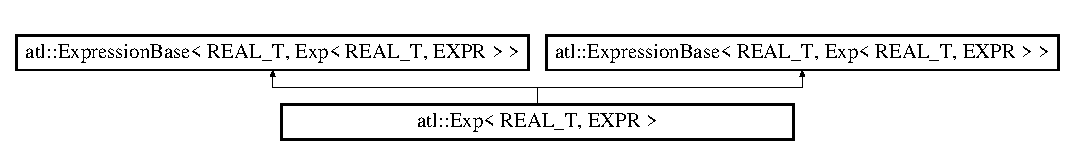
\includegraphics[height=1.642229cm]{structatl_1_1_exp}
\end{center}
\end{figure}
\subsection*{Public Types}
\begin{DoxyCompactItemize}
\item 
\hypertarget{structatl_1_1_exp_a4b49fa63f7f2432f0aa3927aec1aff73}{typedef R\+E\+A\+L\+\_\+\+T {\bfseries B\+A\+S\+E\+\_\+\+T\+Y\+P\+E}}\label{structatl_1_1_exp_a4b49fa63f7f2432f0aa3927aec1aff73}

\item 
\hypertarget{structatl_1_1_exp_a4b49fa63f7f2432f0aa3927aec1aff73}{typedef R\+E\+A\+L\+\_\+\+T {\bfseries B\+A\+S\+E\+\_\+\+T\+Y\+P\+E}}\label{structatl_1_1_exp_a4b49fa63f7f2432f0aa3927aec1aff73}

\end{DoxyCompactItemize}
\subsection*{Public Member Functions}
\begin{DoxyCompactItemize}
\item 
\hypertarget{structatl_1_1_exp_a4fc8871d953fd609370164f42929d736}{{\bfseries Exp} (const \hyperlink{structatl_1_1_expression_base}{Expression\+Base}$<$ R\+E\+A\+L\+\_\+\+T, E\+X\+P\+R $>$ \&a)}\label{structatl_1_1_exp_a4fc8871d953fd609370164f42929d736}

\item 
\hypertarget{structatl_1_1_exp_a4ad5a9a1666163b6e66ecf4865b30e7e}{const R\+E\+A\+L\+\_\+\+T {\bfseries Get\+Value} () const }\label{structatl_1_1_exp_a4ad5a9a1666163b6e66ecf4865b30e7e}

\item 
\hypertarget{structatl_1_1_exp_afbc8958aa71585d44bc767a6b2f62e4f}{const R\+E\+A\+L\+\_\+\+T {\bfseries Get\+Value} (size\+\_\+t i, size\+\_\+t j=0) const }\label{structatl_1_1_exp_afbc8958aa71585d44bc767a6b2f62e4f}

\item 
\hypertarget{structatl_1_1_exp_ac4029416d216ad718ffbb6365f0748f4}{void {\bfseries Push\+Ids} (typename \hyperlink{structatl_1_1_stack_entry}{atl\+::\+Stack\+Entry}$<$ R\+E\+A\+L\+\_\+\+T $>$\+::vi\+\_\+storage \&ids) const }\label{structatl_1_1_exp_ac4029416d216ad718ffbb6365f0748f4}

\item 
\hypertarget{structatl_1_1_exp_a76212b4f0346075224dada55da989326}{void {\bfseries Push\+Ids} (typename \hyperlink{structatl_1_1_stack_entry}{atl\+::\+Stack\+Entry}$<$ R\+E\+A\+L\+\_\+\+T $>$\+::vi\+\_\+storage \&ids, size\+\_\+t i, size\+\_\+t j=0) const }\label{structatl_1_1_exp_a76212b4f0346075224dada55da989326}

\item 
\hypertarget{structatl_1_1_exp_a5dfc68001a2b0ffb7d8a8c6bb08abbec}{const R\+E\+A\+L\+\_\+\+T {\bfseries Evaluate\+Derivative} (uint32\+\_\+t id) const }\label{structatl_1_1_exp_a5dfc68001a2b0ffb7d8a8c6bb08abbec}

\item 
\hypertarget{structatl_1_1_exp_a606ff4e4a554894c19418cbd3cd6b4b3}{R\+E\+A\+L\+\_\+\+T {\bfseries Evaluate\+Derivative} (uint32\+\_\+t a, uint32\+\_\+t b) const }\label{structatl_1_1_exp_a606ff4e4a554894c19418cbd3cd6b4b3}

\item 
\hypertarget{structatl_1_1_exp_ad672b4534d729dbaa1a9a7dd22329289}{R\+E\+A\+L\+\_\+\+T {\bfseries Evaluate\+Derivative} (uint32\+\_\+t x, uint32\+\_\+t y, uint32\+\_\+t z) const }\label{structatl_1_1_exp_ad672b4534d729dbaa1a9a7dd22329289}

\item 
\hypertarget{structatl_1_1_exp_a3982a4c8099fb02234c762d1cd228ae6}{const R\+E\+A\+L\+\_\+\+T {\bfseries Evaluate\+Derivative} (uint32\+\_\+t id, size\+\_\+t i, size\+\_\+t j=0) const }\label{structatl_1_1_exp_a3982a4c8099fb02234c762d1cd228ae6}

\item 
\hypertarget{structatl_1_1_exp_a88db33ccda0675f9cf2efb0e8ed0ba5b}{R\+E\+A\+L\+\_\+\+T {\bfseries Evaluate\+Derivative} (uint32\+\_\+t a, uint32\+\_\+t b, size\+\_\+t i, size\+\_\+t j=0) const }\label{structatl_1_1_exp_a88db33ccda0675f9cf2efb0e8ed0ba5b}

\item 
\hypertarget{structatl_1_1_exp_a58146b72d96dcf551be5a4996911cf7f}{R\+E\+A\+L\+\_\+\+T {\bfseries Evaluate\+Derivative} (uint32\+\_\+t x, uint32\+\_\+t y, uint32\+\_\+t z, size\+\_\+t i, size\+\_\+t j=0) const }\label{structatl_1_1_exp_a58146b72d96dcf551be5a4996911cf7f}

\item 
\hypertarget{structatl_1_1_exp_a3e8da96afc4f14bccbd6d93c4cdcda59}{size\+\_\+t {\bfseries Get\+Columns} () const }\label{structatl_1_1_exp_a3e8da96afc4f14bccbd6d93c4cdcda59}

\item 
\hypertarget{structatl_1_1_exp_a38e06c08362ce93a59211e45447d75de}{size\+\_\+t {\bfseries Get\+Rows} () const }\label{structatl_1_1_exp_a38e06c08362ce93a59211e45447d75de}

\item 
\hypertarget{structatl_1_1_exp_a6b808d05166e359e2adbc4528ff16e25}{bool {\bfseries Is\+Scalar} () const }\label{structatl_1_1_exp_a6b808d05166e359e2adbc4528ff16e25}

\item 
\hyperlink{structatl_1_1_exp_a4fc8871d953fd609370164f42929d736}{Exp} (const \hyperlink{structatl_1_1_expression_base}{Expression\+Base}$<$ R\+E\+A\+L\+\_\+\+T, E\+X\+P\+R $>$ \&a)
\item 
const R\+E\+A\+L\+\_\+\+T \hyperlink{structatl_1_1_exp_a4ad5a9a1666163b6e66ecf4865b30e7e}{Get\+Value} () const 
\item 
const R\+E\+A\+L\+\_\+\+T \hyperlink{structatl_1_1_exp_afbc8958aa71585d44bc767a6b2f62e4f}{Get\+Value} (size\+\_\+t i, size\+\_\+t j=0) const 
\item 
bool \hyperlink{structatl_1_1_exp_a6f7e2607ed8f8e8efe2b5502a2af1650}{Is\+Nonlinear} () const 
\item 
void \hyperlink{structatl_1_1_exp_ac4029416d216ad718ffbb6365f0748f4}{Push\+Ids} (typename \hyperlink{structatl_1_1_stack_entry}{atl\+::\+Stack\+Entry}$<$ R\+E\+A\+L\+\_\+\+T $>$\+::vi\+\_\+storage \&ids) const 
\item 
void \hyperlink{structatl_1_1_exp_a76212b4f0346075224dada55da989326}{Push\+Ids} (typename \hyperlink{structatl_1_1_stack_entry}{atl\+::\+Stack\+Entry}$<$ R\+E\+A\+L\+\_\+\+T $>$\+::vi\+\_\+storage \&ids, size\+\_\+t i, size\+\_\+t j=0) const 
\item 
const R\+E\+A\+L\+\_\+\+T \hyperlink{structatl_1_1_exp_a6e3b08bdc5b3c8ea2cdc0006248edb76}{Evaluate\+Derivative} (uint32\+\_\+t x) const 
\item 
R\+E\+A\+L\+\_\+\+T \hyperlink{structatl_1_1_exp_ae5128016b472aba06bce35bd13369378}{Evaluate\+Derivative} (uint32\+\_\+t x, uint32\+\_\+t y) const 
\item 
R\+E\+A\+L\+\_\+\+T \hyperlink{structatl_1_1_exp_ad672b4534d729dbaa1a9a7dd22329289}{Evaluate\+Derivative} (uint32\+\_\+t x, uint32\+\_\+t y, uint32\+\_\+t z) const 
\item 
const R\+E\+A\+L\+\_\+\+T \hyperlink{structatl_1_1_exp_aa379bdfbffb0c50ce02ab47278d74d3a}{Evaluate\+Derivative} (uint32\+\_\+t x, size\+\_\+t i, size\+\_\+t j=0) const 
\item 
R\+E\+A\+L\+\_\+\+T \hyperlink{structatl_1_1_exp_af80900837e7a13290ac46ef82a555c48}{Evaluate\+Derivative} (uint32\+\_\+t x, uint32\+\_\+t y, size\+\_\+t i, size\+\_\+t j=0) const 
\item 
R\+E\+A\+L\+\_\+\+T \hyperlink{structatl_1_1_exp_a58146b72d96dcf551be5a4996911cf7f}{Evaluate\+Derivative} (uint32\+\_\+t x, uint32\+\_\+t y, uint32\+\_\+t z, size\+\_\+t i, size\+\_\+t j=0) const 
\item 
size\+\_\+t \hyperlink{structatl_1_1_exp_a38e06c08362ce93a59211e45447d75de}{Get\+Rows} () const 
\item 
bool \hyperlink{structatl_1_1_exp_a6b808d05166e359e2adbc4528ff16e25}{Is\+Scalar} () const 
\item 
const std\+::string \hyperlink{structatl_1_1_exp_a07351fca2ccffee1c4c9ae2853991433}{To\+Expression\+Template\+String} () const 
\end{DoxyCompactItemize}
\subsection*{Public Attributes}
\begin{DoxyCompactItemize}
\item 
\hypertarget{structatl_1_1_exp_a30b522a34e15ab6c90764dae3b29fed5}{const E\+X\+P\+R \& {\bfseries expr\+\_\+m}}\label{structatl_1_1_exp_a30b522a34e15ab6c90764dae3b29fed5}

\end{DoxyCompactItemize}


\subsection{Detailed Description}
\subsubsection*{template$<$class R\+E\+A\+L\+\_\+\+T, class E\+X\+P\+R$>$struct atl\+::\+Exp$<$ R\+E\+A\+L\+\_\+\+T, E\+X\+P\+R $>$}

Expression template to handle natural exponential function for variable or container expressions.

$ e^{f(x,y,z)} $

or

$ e^{f_{i,j}(x,y)} $ 

\subsection{Constructor \& Destructor Documentation}
\hypertarget{structatl_1_1_exp_a4fc8871d953fd609370164f42929d736}{\index{atl\+::\+Exp@{atl\+::\+Exp}!Exp@{Exp}}
\index{Exp@{Exp}!atl\+::\+Exp@{atl\+::\+Exp}}
\subsubsection[{Exp}]{\setlength{\rightskip}{0pt plus 5cm}template$<$class R\+E\+A\+L\+\_\+\+T , class E\+X\+P\+R $>$ {\bf atl\+::\+Exp}$<$ R\+E\+A\+L\+\_\+\+T, E\+X\+P\+R $>$\+::{\bf Exp} (
\begin{DoxyParamCaption}
\item[{const {\bf Expression\+Base}$<$ R\+E\+A\+L\+\_\+\+T, E\+X\+P\+R $>$ \&}]{a}
\end{DoxyParamCaption}
)\hspace{0.3cm}{\ttfamily [inline]}}}\label{structatl_1_1_exp_a4fc8871d953fd609370164f42929d736}
Constructor.


\begin{DoxyParams}{Parameters}
{\em a} & \\
\hline
\end{DoxyParams}


\subsection{Member Function Documentation}
\hypertarget{structatl_1_1_exp_a6e3b08bdc5b3c8ea2cdc0006248edb76}{\index{atl\+::\+Exp@{atl\+::\+Exp}!Evaluate\+Derivative@{Evaluate\+Derivative}}
\index{Evaluate\+Derivative@{Evaluate\+Derivative}!atl\+::\+Exp@{atl\+::\+Exp}}
\subsubsection[{Evaluate\+Derivative}]{\setlength{\rightskip}{0pt plus 5cm}template$<$class R\+E\+A\+L\+\_\+\+T , class E\+X\+P\+R $>$ const R\+E\+A\+L\+\_\+\+T {\bf atl\+::\+Exp}$<$ R\+E\+A\+L\+\_\+\+T, E\+X\+P\+R $>$\+::Evaluate\+Derivative (
\begin{DoxyParamCaption}
\item[{uint32\+\_\+t}]{x}
\end{DoxyParamCaption}
) const\hspace{0.3cm}{\ttfamily [inline]}}}\label{structatl_1_1_exp_a6e3b08bdc5b3c8ea2cdc0006248edb76}
Evaluates the first-\/order derivative with respect to x.

$ e^{f(x)}\,\left({{d}\over{d\,x}}\,f(x)\right)$


\begin{DoxyParams}{Parameters}
{\em x} & \\
\hline
\end{DoxyParams}
\begin{DoxyReturn}{Returns}

\end{DoxyReturn}
\hypertarget{structatl_1_1_exp_ae5128016b472aba06bce35bd13369378}{\index{atl\+::\+Exp@{atl\+::\+Exp}!Evaluate\+Derivative@{Evaluate\+Derivative}}
\index{Evaluate\+Derivative@{Evaluate\+Derivative}!atl\+::\+Exp@{atl\+::\+Exp}}
\subsubsection[{Evaluate\+Derivative}]{\setlength{\rightskip}{0pt plus 5cm}template$<$class R\+E\+A\+L\+\_\+\+T , class E\+X\+P\+R $>$ R\+E\+A\+L\+\_\+\+T {\bf atl\+::\+Exp}$<$ R\+E\+A\+L\+\_\+\+T, E\+X\+P\+R $>$\+::Evaluate\+Derivative (
\begin{DoxyParamCaption}
\item[{uint32\+\_\+t}]{x, }
\item[{uint32\+\_\+t}]{y}
\end{DoxyParamCaption}
) const\hspace{0.3cm}{\ttfamily [inline]}}}\label{structatl_1_1_exp_ae5128016b472aba06bce35bd13369378}
Evaluates the second-\/order derivative with respect to x and y.

$ e^{f(x,y)}\,\left({{d}\over{d\,x}}\,f(x,y)\right)\, \left({{d}\over{d\,y}}\,f(x,y)\right)+e^{f(x,y)}\,\left( {{d^2}\over{d\,x\,d\,y}}\,f(x,y)\right) $


\begin{DoxyParams}{Parameters}
{\em x} & \\
\hline
{\em y} & \\
\hline
\end{DoxyParams}
\begin{DoxyReturn}{Returns}

\end{DoxyReturn}
\hypertarget{structatl_1_1_exp_ad672b4534d729dbaa1a9a7dd22329289}{\index{atl\+::\+Exp@{atl\+::\+Exp}!Evaluate\+Derivative@{Evaluate\+Derivative}}
\index{Evaluate\+Derivative@{Evaluate\+Derivative}!atl\+::\+Exp@{atl\+::\+Exp}}
\subsubsection[{Evaluate\+Derivative}]{\setlength{\rightskip}{0pt plus 5cm}template$<$class R\+E\+A\+L\+\_\+\+T , class E\+X\+P\+R $>$ R\+E\+A\+L\+\_\+\+T {\bf atl\+::\+Exp}$<$ R\+E\+A\+L\+\_\+\+T, E\+X\+P\+R $>$\+::Evaluate\+Derivative (
\begin{DoxyParamCaption}
\item[{uint32\+\_\+t}]{x, }
\item[{uint32\+\_\+t}]{y, }
\item[{uint32\+\_\+t}]{z}
\end{DoxyParamCaption}
) const\hspace{0.3cm}{\ttfamily [inline]}}}\label{structatl_1_1_exp_ad672b4534d729dbaa1a9a7dd22329289}
Evaluates the third-\/order derivative with respect to x, y, and z.

$ e^{f\left(x , y , z\right)}\,\left({{d}\over{d\,x}}\,f\left(x , y , z\right)\right)\,\left({{d}\over{d\,y}}\,f\left(x , y , z\right) \right)\,\left({{d}\over{d\,z}}\,f\left(x , y , z\right)\right)+e^{f \left(x , y , z\right)}\,\left({{d^2}\over{d\,x\,d\,y}}\,f\left(x , y , z\right)\right)\,\left({{d}\over{d\,z}}\,f\left(x , y , z\right) \right)+ \\ e^{f\left(x , y , z\right)}\,\left({{d}\over{d\,x}}\,f\left( x , y , z\right)\right)\,\left({{d^2}\over{d\,y\,d\,z}}\,f\left(x , y , z\right)\right)+e^{f\left(x , y , z\right)}\,\left({{d^2}\over{d \,x\,d\,z}}\,f\left(x , y , z\right)\right)\,\left({{d}\over{d\,y}} \,f\left(x , y , z\right)\right)+e^{f\left(x , y , z\right)}\,\left( {{d^3}\over{d\,x\,d\,y\,d\,z}}\,f\left(x , y , z\right)\right) $


\begin{DoxyParams}{Parameters}
{\em x} & \\
\hline
{\em y} & \\
\hline
{\em z} & \\
\hline
\end{DoxyParams}
\begin{DoxyReturn}{Returns}

\end{DoxyReturn}
\hypertarget{structatl_1_1_exp_aa379bdfbffb0c50ce02ab47278d74d3a}{\index{atl\+::\+Exp@{atl\+::\+Exp}!Evaluate\+Derivative@{Evaluate\+Derivative}}
\index{Evaluate\+Derivative@{Evaluate\+Derivative}!atl\+::\+Exp@{atl\+::\+Exp}}
\subsubsection[{Evaluate\+Derivative}]{\setlength{\rightskip}{0pt plus 5cm}template$<$class R\+E\+A\+L\+\_\+\+T , class E\+X\+P\+R $>$ const R\+E\+A\+L\+\_\+\+T {\bf atl\+::\+Exp}$<$ R\+E\+A\+L\+\_\+\+T, E\+X\+P\+R $>$\+::Evaluate\+Derivative (
\begin{DoxyParamCaption}
\item[{uint32\+\_\+t}]{x, }
\item[{size\+\_\+t}]{i, }
\item[{size\+\_\+t}]{j = {\ttfamily 0}}
\end{DoxyParamCaption}
) const\hspace{0.3cm}{\ttfamily [inline]}}}\label{structatl_1_1_exp_aa379bdfbffb0c50ce02ab47278d74d3a}
Evaluates the first-\/order derivative with respect to x at index \{i,j\}.

$ e^{f_{i,j}(x)}\,\left({{d}\over{d\,x}}\,f_{i,j}(x)\right)$


\begin{DoxyParams}{Parameters}
{\em x} & \\
\hline
{\em i} & \\
\hline
{\em j} & \\
\hline
\end{DoxyParams}
\begin{DoxyReturn}{Returns}

\end{DoxyReturn}
\hypertarget{structatl_1_1_exp_af80900837e7a13290ac46ef82a555c48}{\index{atl\+::\+Exp@{atl\+::\+Exp}!Evaluate\+Derivative@{Evaluate\+Derivative}}
\index{Evaluate\+Derivative@{Evaluate\+Derivative}!atl\+::\+Exp@{atl\+::\+Exp}}
\subsubsection[{Evaluate\+Derivative}]{\setlength{\rightskip}{0pt plus 5cm}template$<$class R\+E\+A\+L\+\_\+\+T , class E\+X\+P\+R $>$ R\+E\+A\+L\+\_\+\+T {\bf atl\+::\+Exp}$<$ R\+E\+A\+L\+\_\+\+T, E\+X\+P\+R $>$\+::Evaluate\+Derivative (
\begin{DoxyParamCaption}
\item[{uint32\+\_\+t}]{x, }
\item[{uint32\+\_\+t}]{y, }
\item[{size\+\_\+t}]{i, }
\item[{size\+\_\+t}]{j = {\ttfamily 0}}
\end{DoxyParamCaption}
) const\hspace{0.3cm}{\ttfamily [inline]}}}\label{structatl_1_1_exp_af80900837e7a13290ac46ef82a555c48}
Evaluates the second-\/order derivative with respect to x and y at index \{i,j\}.

$ e^{f_{i,j}(x,y)}\,\left({{d}\over{d\,x}}\,f_{i,j}(x,y)\right)\, \left({{d}\over{d\,y}}\,f_{i,j}(x,y)\right)+e^{f_{i,j}(x,y)}\,\left( {{d^2}\over{d\,x\,d\,y}}\,f_{i,j}(x,y)\right) $


\begin{DoxyParams}{Parameters}
{\em x} & \\
\hline
{\em y} & \\
\hline
{\em i} & \\
\hline
{\em j} & \\
\hline
\end{DoxyParams}
\begin{DoxyReturn}{Returns}

\end{DoxyReturn}
\hypertarget{structatl_1_1_exp_a58146b72d96dcf551be5a4996911cf7f}{\index{atl\+::\+Exp@{atl\+::\+Exp}!Evaluate\+Derivative@{Evaluate\+Derivative}}
\index{Evaluate\+Derivative@{Evaluate\+Derivative}!atl\+::\+Exp@{atl\+::\+Exp}}
\subsubsection[{Evaluate\+Derivative}]{\setlength{\rightskip}{0pt plus 5cm}template$<$class R\+E\+A\+L\+\_\+\+T , class E\+X\+P\+R $>$ R\+E\+A\+L\+\_\+\+T {\bf atl\+::\+Exp}$<$ R\+E\+A\+L\+\_\+\+T, E\+X\+P\+R $>$\+::Evaluate\+Derivative (
\begin{DoxyParamCaption}
\item[{uint32\+\_\+t}]{x, }
\item[{uint32\+\_\+t}]{y, }
\item[{uint32\+\_\+t}]{z, }
\item[{size\+\_\+t}]{i, }
\item[{size\+\_\+t}]{j = {\ttfamily 0}}
\end{DoxyParamCaption}
) const\hspace{0.3cm}{\ttfamily [inline]}}}\label{structatl_1_1_exp_a58146b72d96dcf551be5a4996911cf7f}
Evaluates the third-\/order derivative with respect to x, y, and z at index \{i,j\}.

$ e^{f_{i,j}(x,y,z)}\,\left({{d}\over{d\,x}}\,f_{i,j}(x,y,z)\right)\, \left({{d}\over{d\,y}}\,f_{i,j}(x,y,z)\right)\,\left({{d}\over{d\,z }}\,f_{i,j}(x,y,z)\right)+e^{f_{i,j}(x,y,z)}\,\left({{d^2}\over{d\,x \,d\,y}}\,f_{i,j}(x,y,z)\right)\,\left({{d}\over{d\,z}}\,f_{i,j}(x,y ,z)\right)+ \\ e^{f_{i,j}(x,y,z)}\,\left({{d}\over{d\,x}}\,f_{i,j}(x,y,z )\right)\,\left({{d^2}\over{d\,y\,d\,z}}\,f_{i,j}(x,y,z)\right)+e^{f _{i,j}(x,y,z)}\,\left({{d^2}\over{d\,x\,d\,z}}\,f_{i,j}(x,y,z) \right)\,\left({{d}\over{d\,y}}\,f_{i,j}(x,y,z)\right)+e^{f_{i,j}(x, y,z)}\,\left({{d^3}\over{d\,x\,d\,y\,d\,z}}\,f_{i,j}(x,y,z)\right) $


\begin{DoxyParams}{Parameters}
{\em x} & \\
\hline
{\em y} & \\
\hline
{\em z} & \\
\hline
{\em i} & \\
\hline
{\em j} & \\
\hline
\end{DoxyParams}
\begin{DoxyReturn}{Returns}

\end{DoxyReturn}
\hypertarget{structatl_1_1_exp_a38e06c08362ce93a59211e45447d75de}{\index{atl\+::\+Exp@{atl\+::\+Exp}!Get\+Rows@{Get\+Rows}}
\index{Get\+Rows@{Get\+Rows}!atl\+::\+Exp@{atl\+::\+Exp}}
\subsubsection[{Get\+Rows}]{\setlength{\rightskip}{0pt plus 5cm}template$<$class R\+E\+A\+L\+\_\+\+T , class E\+X\+P\+R $>$ size\+\_\+t {\bf atl\+::\+Exp}$<$ R\+E\+A\+L\+\_\+\+T, E\+X\+P\+R $>$\+::Get\+Rows (
\begin{DoxyParamCaption}
{}
\end{DoxyParamCaption}
) const\hspace{0.3cm}{\ttfamily [inline]}}}\label{structatl_1_1_exp_a38e06c08362ce93a59211e45447d75de}
Return the number of rows.

\begin{DoxyReturn}{Returns}

\end{DoxyReturn}
\hypertarget{structatl_1_1_exp_a4ad5a9a1666163b6e66ecf4865b30e7e}{\index{atl\+::\+Exp@{atl\+::\+Exp}!Get\+Value@{Get\+Value}}
\index{Get\+Value@{Get\+Value}!atl\+::\+Exp@{atl\+::\+Exp}}
\subsubsection[{Get\+Value}]{\setlength{\rightskip}{0pt plus 5cm}template$<$class R\+E\+A\+L\+\_\+\+T , class E\+X\+P\+R $>$ const R\+E\+A\+L\+\_\+\+T {\bf atl\+::\+Exp}$<$ R\+E\+A\+L\+\_\+\+T, E\+X\+P\+R $>$\+::Get\+Value (
\begin{DoxyParamCaption}
{}
\end{DoxyParamCaption}
) const\hspace{0.3cm}{\ttfamily [inline]}}}\label{structatl_1_1_exp_a4ad5a9a1666163b6e66ecf4865b30e7e}
Computes the natural exponential function for the evaluated expression.

\begin{DoxyReturn}{Returns}

\end{DoxyReturn}
\hypertarget{structatl_1_1_exp_afbc8958aa71585d44bc767a6b2f62e4f}{\index{atl\+::\+Exp@{atl\+::\+Exp}!Get\+Value@{Get\+Value}}
\index{Get\+Value@{Get\+Value}!atl\+::\+Exp@{atl\+::\+Exp}}
\subsubsection[{Get\+Value}]{\setlength{\rightskip}{0pt plus 5cm}template$<$class R\+E\+A\+L\+\_\+\+T , class E\+X\+P\+R $>$ const R\+E\+A\+L\+\_\+\+T {\bf atl\+::\+Exp}$<$ R\+E\+A\+L\+\_\+\+T, E\+X\+P\+R $>$\+::Get\+Value (
\begin{DoxyParamCaption}
\item[{size\+\_\+t}]{i, }
\item[{size\+\_\+t}]{j = {\ttfamily 0}}
\end{DoxyParamCaption}
) const\hspace{0.3cm}{\ttfamily [inline]}}}\label{structatl_1_1_exp_afbc8958aa71585d44bc767a6b2f62e4f}
Computes the natural exponential function for the evaluated expression at index \{i,j\}.

\begin{DoxyReturn}{Returns}

\end{DoxyReturn}
\hypertarget{structatl_1_1_exp_a6f7e2607ed8f8e8efe2b5502a2af1650}{\index{atl\+::\+Exp@{atl\+::\+Exp}!Is\+Nonlinear@{Is\+Nonlinear}}
\index{Is\+Nonlinear@{Is\+Nonlinear}!atl\+::\+Exp@{atl\+::\+Exp}}
\subsubsection[{Is\+Nonlinear}]{\setlength{\rightskip}{0pt plus 5cm}template$<$class R\+E\+A\+L\+\_\+\+T , class E\+X\+P\+R $>$ bool {\bf atl\+::\+Exp}$<$ R\+E\+A\+L\+\_\+\+T, E\+X\+P\+R $>$\+::Is\+Nonlinear (
\begin{DoxyParamCaption}
{}
\end{DoxyParamCaption}
) const\hspace{0.3cm}{\ttfamily [inline]}}}\label{structatl_1_1_exp_a6f7e2607ed8f8e8efe2b5502a2af1650}
Returns true.

\begin{DoxyReturn}{Returns}

\end{DoxyReturn}
\hypertarget{structatl_1_1_exp_a6b808d05166e359e2adbc4528ff16e25}{\index{atl\+::\+Exp@{atl\+::\+Exp}!Is\+Scalar@{Is\+Scalar}}
\index{Is\+Scalar@{Is\+Scalar}!atl\+::\+Exp@{atl\+::\+Exp}}
\subsubsection[{Is\+Scalar}]{\setlength{\rightskip}{0pt plus 5cm}template$<$class R\+E\+A\+L\+\_\+\+T , class E\+X\+P\+R $>$ bool {\bf atl\+::\+Exp}$<$ R\+E\+A\+L\+\_\+\+T, E\+X\+P\+R $>$\+::Is\+Scalar (
\begin{DoxyParamCaption}
{}
\end{DoxyParamCaption}
) const\hspace{0.3cm}{\ttfamily [inline]}}}\label{structatl_1_1_exp_a6b808d05166e359e2adbc4528ff16e25}
True if this expression is a scalar.

\begin{DoxyReturn}{Returns}

\end{DoxyReturn}
\hypertarget{structatl_1_1_exp_ac4029416d216ad718ffbb6365f0748f4}{\index{atl\+::\+Exp@{atl\+::\+Exp}!Push\+Ids@{Push\+Ids}}
\index{Push\+Ids@{Push\+Ids}!atl\+::\+Exp@{atl\+::\+Exp}}
\subsubsection[{Push\+Ids}]{\setlength{\rightskip}{0pt plus 5cm}template$<$class R\+E\+A\+L\+\_\+\+T , class E\+X\+P\+R $>$ void {\bf atl\+::\+Exp}$<$ R\+E\+A\+L\+\_\+\+T, E\+X\+P\+R $>$\+::Push\+Ids (
\begin{DoxyParamCaption}
\item[{typename {\bf atl\+::\+Stack\+Entry}$<$ R\+E\+A\+L\+\_\+\+T $>$\+::vi\+\_\+storage \&}]{ids}
\end{DoxyParamCaption}
) const\hspace{0.3cm}{\ttfamily [inline]}}}\label{structatl_1_1_exp_ac4029416d216ad718ffbb6365f0748f4}
Push variable info into a set.


\begin{DoxyParams}{Parameters}
{\em ids} & \\
\hline
\end{DoxyParams}
\hypertarget{structatl_1_1_exp_a76212b4f0346075224dada55da989326}{\index{atl\+::\+Exp@{atl\+::\+Exp}!Push\+Ids@{Push\+Ids}}
\index{Push\+Ids@{Push\+Ids}!atl\+::\+Exp@{atl\+::\+Exp}}
\subsubsection[{Push\+Ids}]{\setlength{\rightskip}{0pt plus 5cm}template$<$class R\+E\+A\+L\+\_\+\+T , class E\+X\+P\+R $>$ void {\bf atl\+::\+Exp}$<$ R\+E\+A\+L\+\_\+\+T, E\+X\+P\+R $>$\+::Push\+Ids (
\begin{DoxyParamCaption}
\item[{typename {\bf atl\+::\+Stack\+Entry}$<$ R\+E\+A\+L\+\_\+\+T $>$\+::vi\+\_\+storage \&}]{ids, }
\item[{size\+\_\+t}]{i, }
\item[{size\+\_\+t}]{j = {\ttfamily 0}}
\end{DoxyParamCaption}
) const\hspace{0.3cm}{\ttfamily [inline]}}}\label{structatl_1_1_exp_a76212b4f0346075224dada55da989326}
Push variable info into a set at index \{i,j\}.


\begin{DoxyParams}{Parameters}
{\em ids} & \\
\hline
{\em i} & \\
\hline
{\em j} & \\
\hline
\end{DoxyParams}
\hypertarget{structatl_1_1_exp_a07351fca2ccffee1c4c9ae2853991433}{\index{atl\+::\+Exp@{atl\+::\+Exp}!To\+Expression\+Template\+String@{To\+Expression\+Template\+String}}
\index{To\+Expression\+Template\+String@{To\+Expression\+Template\+String}!atl\+::\+Exp@{atl\+::\+Exp}}
\subsubsection[{To\+Expression\+Template\+String}]{\setlength{\rightskip}{0pt plus 5cm}template$<$class R\+E\+A\+L\+\_\+\+T , class E\+X\+P\+R $>$ const std\+::string {\bf atl\+::\+Exp}$<$ R\+E\+A\+L\+\_\+\+T, E\+X\+P\+R $>$\+::To\+Expression\+Template\+String (
\begin{DoxyParamCaption}
{}
\end{DoxyParamCaption}
) const\hspace{0.3cm}{\ttfamily [inline]}}}\label{structatl_1_1_exp_a07351fca2ccffee1c4c9ae2853991433}
Create a string representation of this expression template. \begin{DoxyReturn}{Returns}

\end{DoxyReturn}


The documentation for this struct was generated from the following file\+:\begin{DoxyCompactItemize}
\item 
A\+T\+L2/Exp.\+hpp\end{DoxyCompactItemize}

\hypertarget{structatl_1_1_expression_base}{\section{atl\+:\+:Expression\+Base$<$ R\+E\+A\+L\+\_\+\+T, A $>$ Struct Template Reference}
\label{structatl_1_1_expression_base}\index{atl\+::\+Expression\+Base$<$ R\+E\+A\+L\+\_\+\+T, A $>$@{atl\+::\+Expression\+Base$<$ R\+E\+A\+L\+\_\+\+T, A $>$}}
}
\subsection*{Public Member Functions}
\begin{DoxyCompactItemize}
\item 
const A \& \hyperlink{structatl_1_1_expression_base_a48c72f931e64d269c8721f940693ebda}{Cast} () const 
\item 
\hypertarget{structatl_1_1_expression_base_a5f19881cfcf10906ace851129d379bb1}{const R\+E\+A\+L\+\_\+\+T {\bfseries Get\+Value} () const }\label{structatl_1_1_expression_base_a5f19881cfcf10906ace851129d379bb1}

\item 
\hypertarget{structatl_1_1_expression_base_a2e4e10e53867b26cd638cfb588f90a50}{const R\+E\+A\+L\+\_\+\+T {\bfseries Get\+Value} (size\+\_\+t i, size\+\_\+t j=0) const }\label{structatl_1_1_expression_base_a2e4e10e53867b26cd638cfb588f90a50}

\item 
\hypertarget{structatl_1_1_expression_base_af31c04a9315fb7ab8d324f710592f1af}{bool {\bfseries Is\+Nonlinear} () const }\label{structatl_1_1_expression_base_af31c04a9315fb7ab8d324f710592f1af}

\item 
\hypertarget{structatl_1_1_expression_base_a4b69562e0847c41ddcc0dd2cc8b0613b}{void {\bfseries Push\+Ids} (typename \hyperlink{structatl_1_1_stack_entry}{atl\+::\+Stack\+Entry}$<$ R\+E\+A\+L\+\_\+\+T $>$\+::vi\+\_\+storage \&ids) const }\label{structatl_1_1_expression_base_a4b69562e0847c41ddcc0dd2cc8b0613b}

\item 
\hypertarget{structatl_1_1_expression_base_a4810cb822b3ad40d1a8105802e3dcad8}{void {\bfseries Push\+Ids} (typename \hyperlink{structatl_1_1_stack_entry}{atl\+::\+Stack\+Entry}$<$ R\+E\+A\+L\+\_\+\+T $>$\+::vi\+\_\+storage \&ids, size\+\_\+t i, size\+\_\+t j=0) const }\label{structatl_1_1_expression_base_a4810cb822b3ad40d1a8105802e3dcad8}

\item 
\hypertarget{structatl_1_1_expression_base_a88614881ee2f63ec83a6d5dd9d635863}{R\+E\+A\+L\+\_\+\+T {\bfseries Evaluate\+Derivative} (uint32\+\_\+t a) const }\label{structatl_1_1_expression_base_a88614881ee2f63ec83a6d5dd9d635863}

\item 
\hypertarget{structatl_1_1_expression_base_a2e61d3bfdc764f0d16e6eb572b25c363}{R\+E\+A\+L\+\_\+\+T {\bfseries Evaluate\+Derivative} (uint32\+\_\+t a, uint32\+\_\+t b) const }\label{structatl_1_1_expression_base_a2e61d3bfdc764f0d16e6eb572b25c363}

\item 
\hypertarget{structatl_1_1_expression_base_aa1f95c771b199c9a7e4b50812c9403bd}{R\+E\+A\+L\+\_\+\+T {\bfseries Evaluate\+Derivative} (uint32\+\_\+t x, uint32\+\_\+t y, uint32\+\_\+t z) const }\label{structatl_1_1_expression_base_aa1f95c771b199c9a7e4b50812c9403bd}

\item 
\hypertarget{structatl_1_1_expression_base_a0a68467741857a259ac2a7fd20a978b3}{R\+E\+A\+L\+\_\+\+T {\bfseries Evaluate\+Derivative} (uint32\+\_\+t a, size\+\_\+t i, size\+\_\+t j=0) const }\label{structatl_1_1_expression_base_a0a68467741857a259ac2a7fd20a978b3}

\item 
\hypertarget{structatl_1_1_expression_base_a3842851b592ddca24931e79576c4391b}{R\+E\+A\+L\+\_\+\+T {\bfseries Evaluate\+Derivative} (uint32\+\_\+t a, uint32\+\_\+t b, size\+\_\+t i, size\+\_\+t j=0) const }\label{structatl_1_1_expression_base_a3842851b592ddca24931e79576c4391b}

\item 
\hypertarget{structatl_1_1_expression_base_a253be8df62a01657fee080feccfe028e}{R\+E\+A\+L\+\_\+\+T {\bfseries Evaluate\+Derivative} (uint32\+\_\+t x, uint32\+\_\+t y, uint32\+\_\+t z, size\+\_\+t i, size\+\_\+t j=0) const }\label{structatl_1_1_expression_base_a253be8df62a01657fee080feccfe028e}

\item 
\hypertarget{structatl_1_1_expression_base_a6607aa1b435c1b21935cca5bceb4ba82}{const \hyperlink{structatl_1_1_expression_base}{Expression\+Base} \& {\bfseries operator=} (const \hyperlink{structatl_1_1_expression_base}{Expression\+Base} \&exp) const }\label{structatl_1_1_expression_base_a6607aa1b435c1b21935cca5bceb4ba82}

\item 
\hypertarget{structatl_1_1_expression_base_a65be9dccfdbecea0460627d628a533e7}{size\+\_\+t {\bfseries Get\+Columns} () const }\label{structatl_1_1_expression_base_a65be9dccfdbecea0460627d628a533e7}

\item 
\hypertarget{structatl_1_1_expression_base_af1bef71d83cb5cbe01a1b63b041d8563}{size\+\_\+t {\bfseries Get\+Rows} () const }\label{structatl_1_1_expression_base_af1bef71d83cb5cbe01a1b63b041d8563}

\item 
\hypertarget{structatl_1_1_expression_base_a83b116cac0f598f22a2342cc2fdb7214}{bool {\bfseries Is\+Scalar} () const }\label{structatl_1_1_expression_base_a83b116cac0f598f22a2342cc2fdb7214}

\item 
const A \& \hyperlink{structatl_1_1_expression_base_a48c72f931e64d269c8721f940693ebda}{Cast} () const 
\item 
\hypertarget{structatl_1_1_expression_base_a5f19881cfcf10906ace851129d379bb1}{const R\+E\+A\+L\+\_\+\+T {\bfseries Get\+Value} () const }\label{structatl_1_1_expression_base_a5f19881cfcf10906ace851129d379bb1}

\item 
\hypertarget{structatl_1_1_expression_base_a2e4e10e53867b26cd638cfb588f90a50}{const R\+E\+A\+L\+\_\+\+T {\bfseries Get\+Value} (size\+\_\+t i, size\+\_\+t j=0) const }\label{structatl_1_1_expression_base_a2e4e10e53867b26cd638cfb588f90a50}

\item 
\hypertarget{structatl_1_1_expression_base_af31c04a9315fb7ab8d324f710592f1af}{bool {\bfseries Is\+Nonlinear} () const }\label{structatl_1_1_expression_base_af31c04a9315fb7ab8d324f710592f1af}

\item 
\hypertarget{structatl_1_1_expression_base_a4b69562e0847c41ddcc0dd2cc8b0613b}{void {\bfseries Push\+Ids} (typename \hyperlink{structatl_1_1_stack_entry}{atl\+::\+Stack\+Entry}$<$ R\+E\+A\+L\+\_\+\+T $>$\+::vi\+\_\+storage \&ids) const }\label{structatl_1_1_expression_base_a4b69562e0847c41ddcc0dd2cc8b0613b}

\item 
\hypertarget{structatl_1_1_expression_base_a4810cb822b3ad40d1a8105802e3dcad8}{void {\bfseries Push\+Ids} (typename \hyperlink{structatl_1_1_stack_entry}{atl\+::\+Stack\+Entry}$<$ R\+E\+A\+L\+\_\+\+T $>$\+::vi\+\_\+storage \&ids, size\+\_\+t i, size\+\_\+t j=0) const }\label{structatl_1_1_expression_base_a4810cb822b3ad40d1a8105802e3dcad8}

\item 
\hypertarget{structatl_1_1_expression_base_a8d4acaf0df7c5c41f73a81cd09695206}{R\+E\+A\+L\+\_\+\+T {\bfseries Evaluate\+Derivative} (uint32\+\_\+t x) const }\label{structatl_1_1_expression_base_a8d4acaf0df7c5c41f73a81cd09695206}

\item 
\hypertarget{structatl_1_1_expression_base_aa80bf0d6473b57c0e32c4a6c41054542}{R\+E\+A\+L\+\_\+\+T {\bfseries Evaluate\+Derivative} (uint32\+\_\+t x, uint32\+\_\+t y) const }\label{structatl_1_1_expression_base_aa80bf0d6473b57c0e32c4a6c41054542}

\item 
\hypertarget{structatl_1_1_expression_base_aa1f95c771b199c9a7e4b50812c9403bd}{R\+E\+A\+L\+\_\+\+T {\bfseries Evaluate\+Derivative} (uint32\+\_\+t x, uint32\+\_\+t y, uint32\+\_\+t z) const }\label{structatl_1_1_expression_base_aa1f95c771b199c9a7e4b50812c9403bd}

\item 
\hypertarget{structatl_1_1_expression_base_a7e17d01ea0af3917066f0cdd344c0c35}{R\+E\+A\+L\+\_\+\+T {\bfseries Evaluate\+Derivative} (uint32\+\_\+t x, size\+\_\+t i, size\+\_\+t j=0) const }\label{structatl_1_1_expression_base_a7e17d01ea0af3917066f0cdd344c0c35}

\item 
\hypertarget{structatl_1_1_expression_base_aaa68bc54d0a5db9780b0e30df6842047}{R\+E\+A\+L\+\_\+\+T {\bfseries Evaluate\+Derivative} (uint32\+\_\+t x, uint32\+\_\+t y, size\+\_\+t i, size\+\_\+t j=0) const }\label{structatl_1_1_expression_base_aaa68bc54d0a5db9780b0e30df6842047}

\item 
\hypertarget{structatl_1_1_expression_base_a253be8df62a01657fee080feccfe028e}{R\+E\+A\+L\+\_\+\+T {\bfseries Evaluate\+Derivative} (uint32\+\_\+t x, uint32\+\_\+t y, uint32\+\_\+t z, size\+\_\+t i, size\+\_\+t j=0) const }\label{structatl_1_1_expression_base_a253be8df62a01657fee080feccfe028e}

\item 
\hypertarget{structatl_1_1_expression_base_a6607aa1b435c1b21935cca5bceb4ba82}{const \hyperlink{structatl_1_1_expression_base}{Expression\+Base} \& {\bfseries operator=} (const \hyperlink{structatl_1_1_expression_base}{Expression\+Base} \&exp) const }\label{structatl_1_1_expression_base_a6607aa1b435c1b21935cca5bceb4ba82}

\item 
\hypertarget{structatl_1_1_expression_base_a65be9dccfdbecea0460627d628a533e7}{size\+\_\+t {\bfseries Get\+Columns} () const }\label{structatl_1_1_expression_base_a65be9dccfdbecea0460627d628a533e7}

\item 
\hypertarget{structatl_1_1_expression_base_af1bef71d83cb5cbe01a1b63b041d8563}{size\+\_\+t {\bfseries Get\+Rows} () const }\label{structatl_1_1_expression_base_af1bef71d83cb5cbe01a1b63b041d8563}

\item 
\hypertarget{structatl_1_1_expression_base_a83b116cac0f598f22a2342cc2fdb7214}{bool {\bfseries Is\+Scalar} () const }\label{structatl_1_1_expression_base_a83b116cac0f598f22a2342cc2fdb7214}

\item 
std\+::string \hyperlink{structatl_1_1_expression_base_a8bb3985f35c1f4b805dd7658127cc85c}{To\+Expression\+Template\+String} () const 
\end{DoxyCompactItemize}


\subsection{Member Function Documentation}
\hypertarget{structatl_1_1_expression_base_a48c72f931e64d269c8721f940693ebda}{\index{atl\+::\+Expression\+Base@{atl\+::\+Expression\+Base}!Cast@{Cast}}
\index{Cast@{Cast}!atl\+::\+Expression\+Base@{atl\+::\+Expression\+Base}}
\subsubsection[{Cast}]{\setlength{\rightskip}{0pt plus 5cm}template$<$class R\+E\+A\+L\+\_\+\+T, class A$>$ const A\& {\bf atl\+::\+Expression\+Base}$<$ R\+E\+A\+L\+\_\+\+T, A $>$\+::Cast (
\begin{DoxyParamCaption}
{}
\end{DoxyParamCaption}
) const\hspace{0.3cm}{\ttfamily [inline]}}}\label{structatl_1_1_expression_base_a48c72f931e64d269c8721f940693ebda}
Cast this expression template to it's child representation.

\begin{DoxyReturn}{Returns}

\end{DoxyReturn}


Referenced by atl\+::acos(), atl\+::asin(), atl\+::atan(), atl\+::ceil(), atl\+::cos(), atl\+::cosh(), atl\+::floor(), atl\+::log(), atl\+::log10(), atl\+::operator$\ast$(), atl\+::operator+(), atl\+::operator-\/(), atl\+::operator/(), atl\+::pow(), atl\+::sin(), atl\+::sinh(), atl\+::sqrt(), atl\+::tan(), atl\+::tanh(), and atl\+::\+Expression\+Base$<$ R\+E\+A\+L\+\_\+\+T, Add$<$ R\+E\+A\+L\+\_\+\+T, L\+H\+S, R\+H\+S $>$ $>$\+::\+To\+Expression\+Template\+String().

\hypertarget{structatl_1_1_expression_base_a48c72f931e64d269c8721f940693ebda}{\index{atl\+::\+Expression\+Base@{atl\+::\+Expression\+Base}!Cast@{Cast}}
\index{Cast@{Cast}!atl\+::\+Expression\+Base@{atl\+::\+Expression\+Base}}
\subsubsection[{Cast}]{\setlength{\rightskip}{0pt plus 5cm}template$<$class R\+E\+A\+L\+\_\+\+T, class A$>$ const A\& {\bf atl\+::\+Expression\+Base}$<$ R\+E\+A\+L\+\_\+\+T, A $>$\+::Cast (
\begin{DoxyParamCaption}
{}
\end{DoxyParamCaption}
) const\hspace{0.3cm}{\ttfamily [inline]}}}\label{structatl_1_1_expression_base_a48c72f931e64d269c8721f940693ebda}
Cast this expression template to it's child representation.

\begin{DoxyReturn}{Returns}

\end{DoxyReturn}
\hypertarget{structatl_1_1_expression_base_a8bb3985f35c1f4b805dd7658127cc85c}{\index{atl\+::\+Expression\+Base@{atl\+::\+Expression\+Base}!To\+Expression\+Template\+String@{To\+Expression\+Template\+String}}
\index{To\+Expression\+Template\+String@{To\+Expression\+Template\+String}!atl\+::\+Expression\+Base@{atl\+::\+Expression\+Base}}
\subsubsection[{To\+Expression\+Template\+String}]{\setlength{\rightskip}{0pt plus 5cm}template$<$class R\+E\+A\+L\+\_\+\+T, class A$>$ std\+::string {\bf atl\+::\+Expression\+Base}$<$ R\+E\+A\+L\+\_\+\+T, A $>$\+::To\+Expression\+Template\+String (
\begin{DoxyParamCaption}
{}
\end{DoxyParamCaption}
) const\hspace{0.3cm}{\ttfamily [inline]}}}\label{structatl_1_1_expression_base_a8bb3985f35c1f4b805dd7658127cc85c}
Create a string representation of this expression template. \begin{DoxyReturn}{Returns}

\end{DoxyReturn}


The documentation for this struct was generated from the following file\+:\begin{DoxyCompactItemize}
\item 
A\+T\+L2/Expression.\+hpp\end{DoxyCompactItemize}

\hypertarget{structatl_1_1_expression_trait}{\section{atl\+:\+:Expression\+Trait$<$ T $>$ Struct Template Reference}
\label{structatl_1_1_expression_trait}\index{atl\+::\+Expression\+Trait$<$ T $>$@{atl\+::\+Expression\+Trait$<$ T $>$}}
}
\subsection*{Public Member Functions}
\begin{DoxyCompactItemize}
\item 
\hypertarget{structatl_1_1_expression_trait_ab387a6b859a0f734b5b35ff90ca12f06}{{\footnotesize template$<$$>$ }\\Expression\+Type {\bfseries et\+\_\+type}}\label{structatl_1_1_expression_trait_ab387a6b859a0f734b5b35ff90ca12f06}

\item 
\hypertarget{structatl_1_1_expression_trait_a623a8baffc6a22b5f13e4a3c73e2df22}{{\footnotesize template$<$$>$ }\\Expression\+Type {\bfseries et\+\_\+type}}\label{structatl_1_1_expression_trait_a623a8baffc6a22b5f13e4a3c73e2df22}

\item 
\hypertarget{structatl_1_1_expression_trait_ac22f1cf782c1d22a113910e2f0b149de}{{\footnotesize template$<$$>$ }\\Expression\+Type {\bfseries et\+\_\+type}}\label{structatl_1_1_expression_trait_ac22f1cf782c1d22a113910e2f0b149de}

\item 
\hypertarget{structatl_1_1_expression_trait_ab387a6b859a0f734b5b35ff90ca12f06}{{\footnotesize template$<$$>$ }\\Expression\+Type {\bfseries et\+\_\+type}}\label{structatl_1_1_expression_trait_ab387a6b859a0f734b5b35ff90ca12f06}

\item 
\hypertarget{structatl_1_1_expression_trait_a623a8baffc6a22b5f13e4a3c73e2df22}{{\footnotesize template$<$$>$ }\\Expression\+Type {\bfseries et\+\_\+type}}\label{structatl_1_1_expression_trait_a623a8baffc6a22b5f13e4a3c73e2df22}

\item 
\hypertarget{structatl_1_1_expression_trait_ac22f1cf782c1d22a113910e2f0b149de}{{\footnotesize template$<$$>$ }\\Expression\+Type {\bfseries et\+\_\+type}}\label{structatl_1_1_expression_trait_ac22f1cf782c1d22a113910e2f0b149de}

\end{DoxyCompactItemize}
\subsection*{Static Public Attributes}
\begin{DoxyCompactItemize}
\item 
\hypertarget{structatl_1_1_expression_trait_a93b91ffbf84ec07dcc0084ddddf0a7d3}{static Expression\+Type {\bfseries et\+\_\+type} = E\+T\+\_\+\+B\+A\+S\+E}\label{structatl_1_1_expression_trait_a93b91ffbf84ec07dcc0084ddddf0a7d3}

\end{DoxyCompactItemize}


The documentation for this struct was generated from the following file\+:\begin{DoxyCompactItemize}
\item 
A\+T\+L2/Expression.\+hpp\end{DoxyCompactItemize}

\hypertarget{structatl_1_1_fabs}{\section{atl\+:\+:Fabs$<$ R\+E\+A\+L\+\_\+\+T, E\+X\+P\+R $>$ Struct Template Reference}
\label{structatl_1_1_fabs}\index{atl\+::\+Fabs$<$ R\+E\+A\+L\+\_\+\+T, E\+X\+P\+R $>$@{atl\+::\+Fabs$<$ R\+E\+A\+L\+\_\+\+T, E\+X\+P\+R $>$}}
}


{\ttfamily \#include $<$Fabs.\+hpp$>$}

Inheritance diagram for atl\+:\+:Fabs$<$ R\+E\+A\+L\+\_\+\+T, E\+X\+P\+R $>$\+:\begin{figure}[H]
\begin{center}
\leavevmode
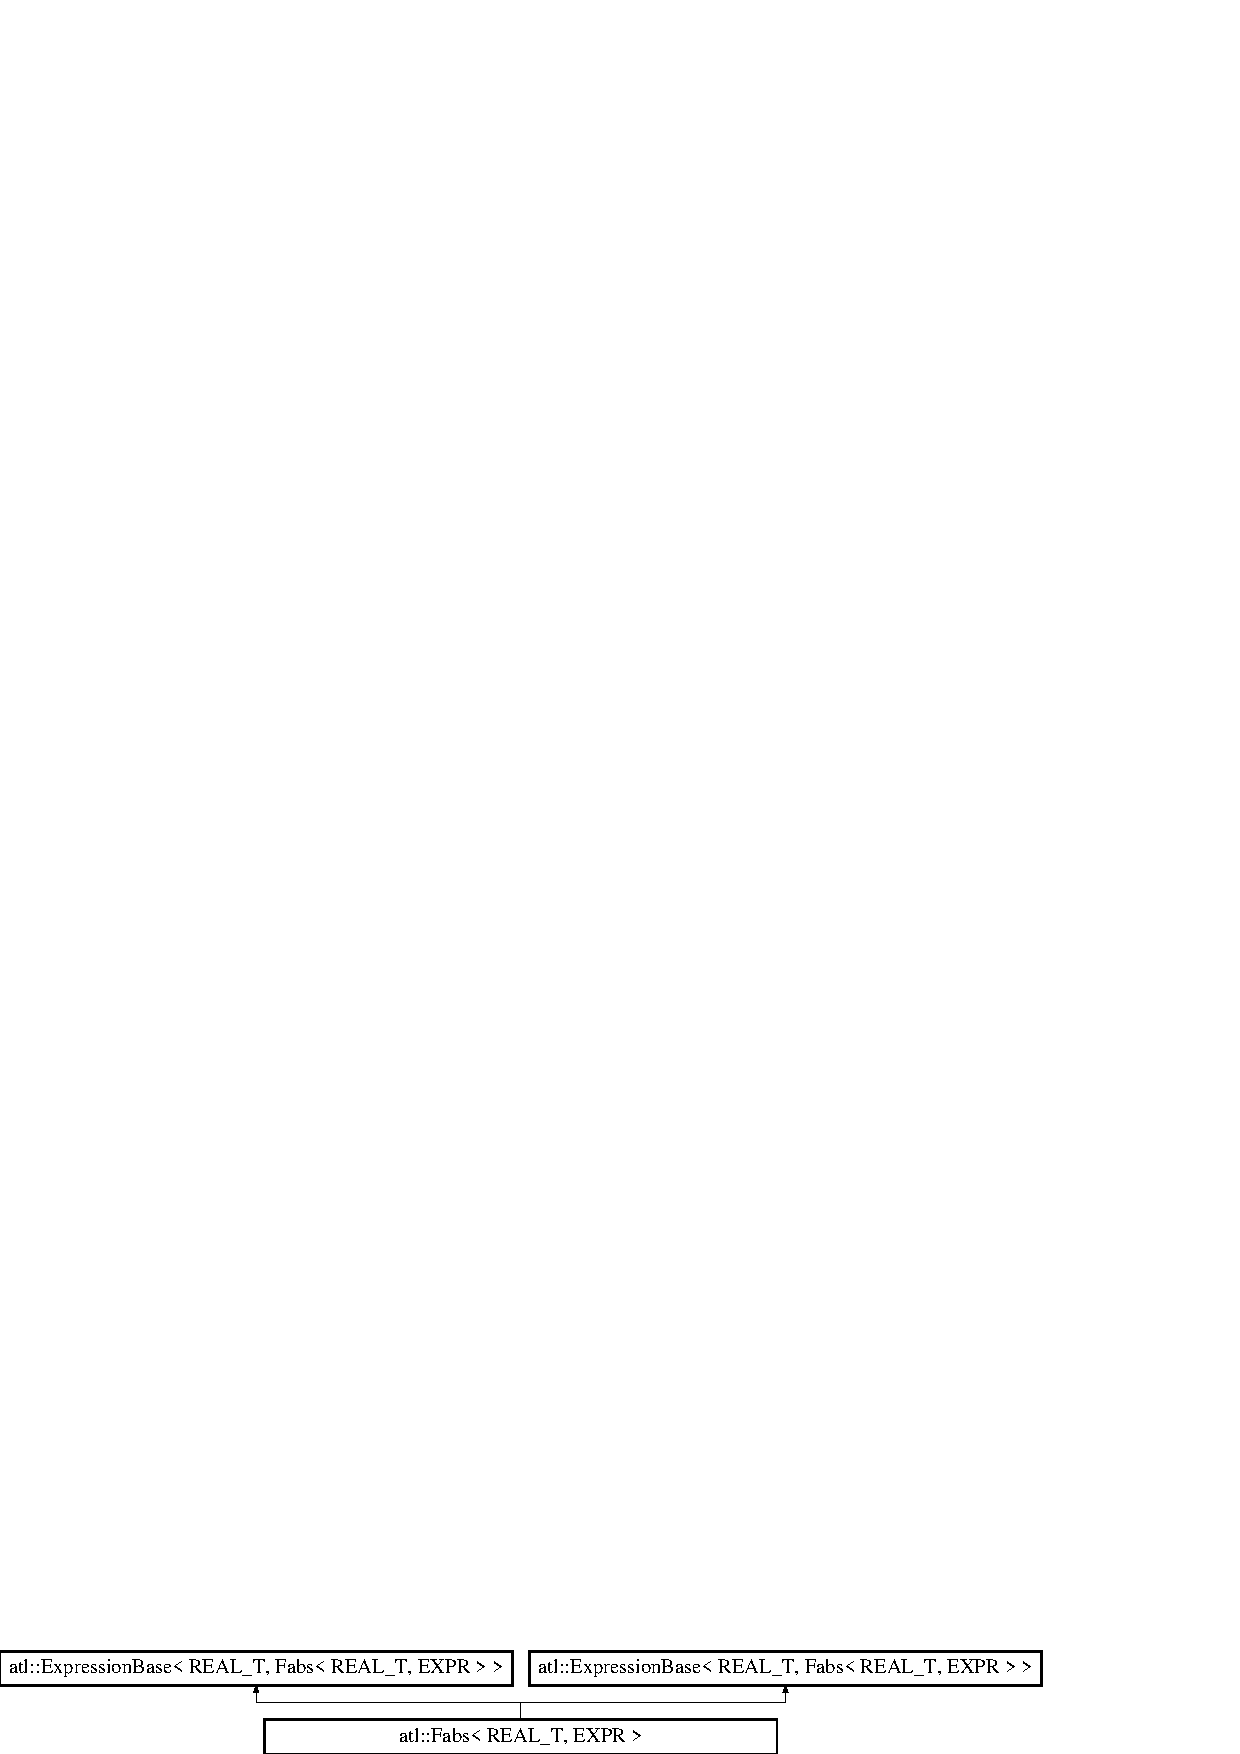
\includegraphics[height=1.609195cm]{structatl_1_1_fabs}
\end{center}
\end{figure}
\subsection*{Public Types}
\begin{DoxyCompactItemize}
\item 
\hypertarget{structatl_1_1_fabs_a011b0506fdd75f1e593b1bb884fc95e2}{typedef R\+E\+A\+L\+\_\+\+T {\bfseries B\+A\+S\+E\+\_\+\+T\+Y\+P\+E}}\label{structatl_1_1_fabs_a011b0506fdd75f1e593b1bb884fc95e2}

\item 
\hypertarget{structatl_1_1_fabs_a011b0506fdd75f1e593b1bb884fc95e2}{typedef R\+E\+A\+L\+\_\+\+T {\bfseries B\+A\+S\+E\+\_\+\+T\+Y\+P\+E}}\label{structatl_1_1_fabs_a011b0506fdd75f1e593b1bb884fc95e2}

\end{DoxyCompactItemize}
\subsection*{Public Member Functions}
\begin{DoxyCompactItemize}
\item 
\hypertarget{structatl_1_1_fabs_a209f2e5eef31610984955cc8c397a31b}{{\bfseries Fabs} (const \hyperlink{structatl_1_1_expression_base}{Expression\+Base}$<$ R\+E\+A\+L\+\_\+\+T, E\+X\+P\+R $>$ \&a)}\label{structatl_1_1_fabs_a209f2e5eef31610984955cc8c397a31b}

\item 
\hypertarget{structatl_1_1_fabs_ac8ccc3d35e00f868a9d72cd7427005aa}{const R\+E\+A\+L\+\_\+\+T {\bfseries Get\+Value} () const }\label{structatl_1_1_fabs_ac8ccc3d35e00f868a9d72cd7427005aa}

\item 
\hypertarget{structatl_1_1_fabs_ac3ab5f58693e26604421c4705b8e26e5}{const R\+E\+A\+L\+\_\+\+T {\bfseries Get\+Value} (size\+\_\+t i, size\+\_\+t j=0) const }\label{structatl_1_1_fabs_ac3ab5f58693e26604421c4705b8e26e5}

\item 
\hypertarget{structatl_1_1_fabs_a515bb4e9b6c9aa45771a1e9d171b0874}{void {\bfseries Push\+Ids} (typename \hyperlink{structatl_1_1_stack_entry}{atl\+::\+Stack\+Entry}$<$ R\+E\+A\+L\+\_\+\+T $>$\+::vi\+\_\+storage \&ids) const }\label{structatl_1_1_fabs_a515bb4e9b6c9aa45771a1e9d171b0874}

\item 
\hypertarget{structatl_1_1_fabs_a6591506f92da3e4526865b0ac0362e9d}{void {\bfseries Push\+Ids} (typename \hyperlink{structatl_1_1_stack_entry}{atl\+::\+Stack\+Entry}$<$ R\+E\+A\+L\+\_\+\+T $>$\+::vi\+\_\+storage \&ids, size\+\_\+t i, size\+\_\+t j=0) const }\label{structatl_1_1_fabs_a6591506f92da3e4526865b0ac0362e9d}

\item 
\hypertarget{structatl_1_1_fabs_a8c6e6aec1dd8045f4b9b99633c4da571}{const R\+E\+A\+L\+\_\+\+T {\bfseries Evaluate\+Derivative} (uint32\+\_\+t id) const }\label{structatl_1_1_fabs_a8c6e6aec1dd8045f4b9b99633c4da571}

\item 
\hypertarget{structatl_1_1_fabs_a698c05a67f7731ddfda90486771bbf81}{R\+E\+A\+L\+\_\+\+T {\bfseries Evaluate\+Derivative} (uint32\+\_\+t a, uint32\+\_\+t b) const }\label{structatl_1_1_fabs_a698c05a67f7731ddfda90486771bbf81}

\item 
\hypertarget{structatl_1_1_fabs_abfd108ac8bacee559ba29b9a3a89782b}{R\+E\+A\+L\+\_\+\+T {\bfseries Evaluate\+Derivative} (uint32\+\_\+t x, uint32\+\_\+t y, uint32\+\_\+t z) const }\label{structatl_1_1_fabs_abfd108ac8bacee559ba29b9a3a89782b}

\item 
\hypertarget{structatl_1_1_fabs_a6035b38438d888139da7359d2b6a80db}{const R\+E\+A\+L\+\_\+\+T {\bfseries Evaluate\+Derivative} (uint32\+\_\+t id, size\+\_\+t i, size\+\_\+t j=0) const }\label{structatl_1_1_fabs_a6035b38438d888139da7359d2b6a80db}

\item 
\hypertarget{structatl_1_1_fabs_a5ee04c4647524a4ecb99a2265b644aea}{R\+E\+A\+L\+\_\+\+T {\bfseries Evaluate\+Derivative} (uint32\+\_\+t a, uint32\+\_\+t b, size\+\_\+t i, size\+\_\+t j=0) const }\label{structatl_1_1_fabs_a5ee04c4647524a4ecb99a2265b644aea}

\item 
\hypertarget{structatl_1_1_fabs_a84ba8df8b0dfe44681db684598b5a134}{R\+E\+A\+L\+\_\+\+T {\bfseries Evaluate\+Derivative} (uint32\+\_\+t x, uint32\+\_\+t y, uint32\+\_\+t z, size\+\_\+t i, size\+\_\+t j=0) const }\label{structatl_1_1_fabs_a84ba8df8b0dfe44681db684598b5a134}

\item 
\hypertarget{structatl_1_1_fabs_abee5b788d8185ba11fcdca15f7171617}{size\+\_\+t {\bfseries Get\+Columns} () const }\label{structatl_1_1_fabs_abee5b788d8185ba11fcdca15f7171617}

\item 
\hypertarget{structatl_1_1_fabs_a34d34b2066fea0f12831e4d328d0bf02}{size\+\_\+t {\bfseries Get\+Rows} () const }\label{structatl_1_1_fabs_a34d34b2066fea0f12831e4d328d0bf02}

\item 
\hypertarget{structatl_1_1_fabs_ada0a07c884510106cc0ac10cc49ff422}{bool {\bfseries Is\+Scalar} () const }\label{structatl_1_1_fabs_ada0a07c884510106cc0ac10cc49ff422}

\item 
\hyperlink{structatl_1_1_fabs_a209f2e5eef31610984955cc8c397a31b}{Fabs} (const \hyperlink{structatl_1_1_expression_base}{Expression\+Base}$<$ R\+E\+A\+L\+\_\+\+T, E\+X\+P\+R $>$ \&a)
\item 
const R\+E\+A\+L\+\_\+\+T \hyperlink{structatl_1_1_fabs_ac8ccc3d35e00f868a9d72cd7427005aa}{Get\+Value} () const 
\item 
const R\+E\+A\+L\+\_\+\+T \hyperlink{structatl_1_1_fabs_ac3ab5f58693e26604421c4705b8e26e5}{Get\+Value} (size\+\_\+t i, size\+\_\+t j=0) const 
\item 
bool \hyperlink{structatl_1_1_fabs_a10e7071a17ffa1319f200569a1b22ade}{Is\+Nonlinear} () const 
\item 
void \hyperlink{structatl_1_1_fabs_a515bb4e9b6c9aa45771a1e9d171b0874}{Push\+Ids} (typename \hyperlink{structatl_1_1_stack_entry}{atl\+::\+Stack\+Entry}$<$ R\+E\+A\+L\+\_\+\+T $>$\+::vi\+\_\+storage \&ids) const 
\item 
void \hyperlink{structatl_1_1_fabs_a6591506f92da3e4526865b0ac0362e9d}{Push\+Ids} (typename \hyperlink{structatl_1_1_stack_entry}{atl\+::\+Stack\+Entry}$<$ R\+E\+A\+L\+\_\+\+T $>$\+::vi\+\_\+storage \&ids, size\+\_\+t i, size\+\_\+t j=0) const 
\item 
const R\+E\+A\+L\+\_\+\+T \hyperlink{structatl_1_1_fabs_affe4a7b048c33b8e0ae05186b1a52086}{Evaluate\+Derivative} (uint32\+\_\+t x) const 
\item 
R\+E\+A\+L\+\_\+\+T \hyperlink{structatl_1_1_fabs_abf10b45ec3e8c295bec9f9f4acc0f30d}{Evaluate\+Derivative} (uint32\+\_\+t x, uint32\+\_\+t y) const 
\item 
R\+E\+A\+L\+\_\+\+T \hyperlink{structatl_1_1_fabs_abfd108ac8bacee559ba29b9a3a89782b}{Evaluate\+Derivative} (uint32\+\_\+t x, uint32\+\_\+t y, uint32\+\_\+t z) const 
\item 
const R\+E\+A\+L\+\_\+\+T \hyperlink{structatl_1_1_fabs_ad9f2521ad8de8ecc5f5c2becda8cdc5a}{Evaluate\+Derivative} (uint32\+\_\+t x, size\+\_\+t i, size\+\_\+t j=0) const 
\item 
R\+E\+A\+L\+\_\+\+T \hyperlink{structatl_1_1_fabs_a95bda969d49d5b5b67b3a195cb6a77f7}{Evaluate\+Derivative} (uint32\+\_\+t x, uint32\+\_\+t y, size\+\_\+t i, size\+\_\+t j=0) const 
\item 
R\+E\+A\+L\+\_\+\+T \hyperlink{structatl_1_1_fabs_a84ba8df8b0dfe44681db684598b5a134}{Evaluate\+Derivative} (uint32\+\_\+t x, uint32\+\_\+t y, uint32\+\_\+t z, size\+\_\+t i, size\+\_\+t j=0) const 
\item 
size\+\_\+t \hyperlink{structatl_1_1_fabs_a34d34b2066fea0f12831e4d328d0bf02}{Get\+Rows} () const 
\item 
bool \hyperlink{structatl_1_1_fabs_ada0a07c884510106cc0ac10cc49ff422}{Is\+Scalar} () const 
\item 
const std\+::string \hyperlink{structatl_1_1_fabs_aefc940a9b227fbc1af622a12c3255583}{To\+Expression\+Template\+String} () const 
\end{DoxyCompactItemize}
\subsection*{Public Attributes}
\begin{DoxyCompactItemize}
\item 
\hypertarget{structatl_1_1_fabs_a81fa41c846dc0a9bec57195a9693b5fb}{const E\+X\+P\+R \& {\bfseries expr\+\_\+m}}\label{structatl_1_1_fabs_a81fa41c846dc0a9bec57195a9693b5fb}

\end{DoxyCompactItemize}


\subsection{Detailed Description}
\subsubsection*{template$<$class R\+E\+A\+L\+\_\+\+T, class E\+X\+P\+R$>$struct atl\+::\+Fabs$<$ R\+E\+A\+L\+\_\+\+T, E\+X\+P\+R $>$}

Expression template to handle the absolute value for variable or container expressions. Not differentiable at zero. For a differentiable estimate see \hyperlink{namespaceatl_a3b7620eadb39267aa49f9ab580bd03e9}{ad\+\_\+fabs}.

$ \arccos f(x,y) $

or

$ \arccos f_{i,j}(x,y) $ 

\subsection{Constructor \& Destructor Documentation}
\hypertarget{structatl_1_1_fabs_a209f2e5eef31610984955cc8c397a31b}{\index{atl\+::\+Fabs@{atl\+::\+Fabs}!Fabs@{Fabs}}
\index{Fabs@{Fabs}!atl\+::\+Fabs@{atl\+::\+Fabs}}
\subsubsection[{Fabs}]{\setlength{\rightskip}{0pt plus 5cm}template$<$class R\+E\+A\+L\+\_\+\+T , class E\+X\+P\+R $>$ {\bf atl\+::\+Fabs}$<$ R\+E\+A\+L\+\_\+\+T, E\+X\+P\+R $>$\+::{\bf Fabs} (
\begin{DoxyParamCaption}
\item[{const {\bf Expression\+Base}$<$ R\+E\+A\+L\+\_\+\+T, E\+X\+P\+R $>$ \&}]{a}
\end{DoxyParamCaption}
)\hspace{0.3cm}{\ttfamily [inline]}}}\label{structatl_1_1_fabs_a209f2e5eef31610984955cc8c397a31b}
Constructor


\begin{DoxyParams}{Parameters}
{\em a} & \\
\hline
\end{DoxyParams}


\subsection{Member Function Documentation}
\hypertarget{structatl_1_1_fabs_affe4a7b048c33b8e0ae05186b1a52086}{\index{atl\+::\+Fabs@{atl\+::\+Fabs}!Evaluate\+Derivative@{Evaluate\+Derivative}}
\index{Evaluate\+Derivative@{Evaluate\+Derivative}!atl\+::\+Fabs@{atl\+::\+Fabs}}
\subsubsection[{Evaluate\+Derivative}]{\setlength{\rightskip}{0pt plus 5cm}template$<$class R\+E\+A\+L\+\_\+\+T , class E\+X\+P\+R $>$ const R\+E\+A\+L\+\_\+\+T {\bf atl\+::\+Fabs}$<$ R\+E\+A\+L\+\_\+\+T, E\+X\+P\+R $>$\+::Evaluate\+Derivative (
\begin{DoxyParamCaption}
\item[{uint32\+\_\+t}]{x}
\end{DoxyParamCaption}
) const\hspace{0.3cm}{\ttfamily [inline]}}}\label{structatl_1_1_fabs_affe4a7b048c33b8e0ae05186b1a52086}
Evaluates the first-\/order derivative with respect to x.

$ {{f(x)\,\left({{d}\over{d\,x}}\,f(x)\right)}\over{ \left| f(x)\right| }} $

note\+: undefined at f(x) = 0. see \hyperlink{namespaceatl_a3b7620eadb39267aa49f9ab580bd03e9}{ad\+\_\+fabs} for an alternative.


\begin{DoxyParams}{Parameters}
{\em x} & \\
\hline
\end{DoxyParams}
\begin{DoxyReturn}{Returns}

\end{DoxyReturn}
\hypertarget{structatl_1_1_fabs_abf10b45ec3e8c295bec9f9f4acc0f30d}{\index{atl\+::\+Fabs@{atl\+::\+Fabs}!Evaluate\+Derivative@{Evaluate\+Derivative}}
\index{Evaluate\+Derivative@{Evaluate\+Derivative}!atl\+::\+Fabs@{atl\+::\+Fabs}}
\subsubsection[{Evaluate\+Derivative}]{\setlength{\rightskip}{0pt plus 5cm}template$<$class R\+E\+A\+L\+\_\+\+T , class E\+X\+P\+R $>$ R\+E\+A\+L\+\_\+\+T {\bf atl\+::\+Fabs}$<$ R\+E\+A\+L\+\_\+\+T, E\+X\+P\+R $>$\+::Evaluate\+Derivative (
\begin{DoxyParamCaption}
\item[{uint32\+\_\+t}]{x, }
\item[{uint32\+\_\+t}]{y}
\end{DoxyParamCaption}
) const\hspace{0.3cm}{\ttfamily [inline]}}}\label{structatl_1_1_fabs_abf10b45ec3e8c295bec9f9f4acc0f30d}
Evaluates the second-\/order derivative with respect to x and y.

$ {{f(x,y)\,\left({{d^2}\over{d\,x\,d\,y}}\,f(x,y)\right) }\over{\left| f(x,y)\right| }} $


\begin{DoxyParams}{Parameters}
{\em x} & \\
\hline
{\em y} & \\
\hline
\end{DoxyParams}
\begin{DoxyReturn}{Returns}

\end{DoxyReturn}
\hypertarget{structatl_1_1_fabs_abfd108ac8bacee559ba29b9a3a89782b}{\index{atl\+::\+Fabs@{atl\+::\+Fabs}!Evaluate\+Derivative@{Evaluate\+Derivative}}
\index{Evaluate\+Derivative@{Evaluate\+Derivative}!atl\+::\+Fabs@{atl\+::\+Fabs}}
\subsubsection[{Evaluate\+Derivative}]{\setlength{\rightskip}{0pt plus 5cm}template$<$class R\+E\+A\+L\+\_\+\+T , class E\+X\+P\+R $>$ R\+E\+A\+L\+\_\+\+T {\bf atl\+::\+Fabs}$<$ R\+E\+A\+L\+\_\+\+T, E\+X\+P\+R $>$\+::Evaluate\+Derivative (
\begin{DoxyParamCaption}
\item[{uint32\+\_\+t}]{x, }
\item[{uint32\+\_\+t}]{y, }
\item[{uint32\+\_\+t}]{z}
\end{DoxyParamCaption}
) const\hspace{0.3cm}{\ttfamily [inline]}}}\label{structatl_1_1_fabs_abfd108ac8bacee559ba29b9a3a89782b}
Evaluates the third-\/order derivative with respect to x, y, and z at index \{i,j\}.

$ {{f(x,y,z)\,\left({{d^3}\over{d\,x\,d\,y\,d\,z}}\,f(x,y ,z)\right)}\over{\left| f(x,y,z)\right| }} $

note\+: undefined at f(x) = 0. see \hyperlink{namespaceatl_a3b7620eadb39267aa49f9ab580bd03e9}{ad\+\_\+fabs} for an alternative.


\begin{DoxyParams}{Parameters}
{\em x} & \\
\hline
{\em y} & \\
\hline
{\em z} & \\
\hline
\end{DoxyParams}
\begin{DoxyReturn}{Returns}

\end{DoxyReturn}
\hypertarget{structatl_1_1_fabs_ad9f2521ad8de8ecc5f5c2becda8cdc5a}{\index{atl\+::\+Fabs@{atl\+::\+Fabs}!Evaluate\+Derivative@{Evaluate\+Derivative}}
\index{Evaluate\+Derivative@{Evaluate\+Derivative}!atl\+::\+Fabs@{atl\+::\+Fabs}}
\subsubsection[{Evaluate\+Derivative}]{\setlength{\rightskip}{0pt plus 5cm}template$<$class R\+E\+A\+L\+\_\+\+T , class E\+X\+P\+R $>$ const R\+E\+A\+L\+\_\+\+T {\bf atl\+::\+Fabs}$<$ R\+E\+A\+L\+\_\+\+T, E\+X\+P\+R $>$\+::Evaluate\+Derivative (
\begin{DoxyParamCaption}
\item[{uint32\+\_\+t}]{x, }
\item[{size\+\_\+t}]{i, }
\item[{size\+\_\+t}]{j = {\ttfamily 0}}
\end{DoxyParamCaption}
) const\hspace{0.3cm}{\ttfamily [inline]}}}\label{structatl_1_1_fabs_ad9f2521ad8de8ecc5f5c2becda8cdc5a}
Evaluates the first-\/order derivative with respect to x at index \{i,j\}.

$ {{f_{i,j}(x)\,\left({{d}\over{d\,x}}\,f_{i,j}(x)\right)}\over{ \left| f_{i,j}(x)\right| }} $

note\+: undefined at f(x) = 0. see \hyperlink{namespaceatl_a3b7620eadb39267aa49f9ab580bd03e9}{ad\+\_\+fabs} for an alternative.


\begin{DoxyParams}{Parameters}
{\em x} & \\
\hline
\end{DoxyParams}
\begin{DoxyReturn}{Returns}

\end{DoxyReturn}
\hypertarget{structatl_1_1_fabs_a95bda969d49d5b5b67b3a195cb6a77f7}{\index{atl\+::\+Fabs@{atl\+::\+Fabs}!Evaluate\+Derivative@{Evaluate\+Derivative}}
\index{Evaluate\+Derivative@{Evaluate\+Derivative}!atl\+::\+Fabs@{atl\+::\+Fabs}}
\subsubsection[{Evaluate\+Derivative}]{\setlength{\rightskip}{0pt plus 5cm}template$<$class R\+E\+A\+L\+\_\+\+T , class E\+X\+P\+R $>$ R\+E\+A\+L\+\_\+\+T {\bf atl\+::\+Fabs}$<$ R\+E\+A\+L\+\_\+\+T, E\+X\+P\+R $>$\+::Evaluate\+Derivative (
\begin{DoxyParamCaption}
\item[{uint32\+\_\+t}]{x, }
\item[{uint32\+\_\+t}]{y, }
\item[{size\+\_\+t}]{i, }
\item[{size\+\_\+t}]{j = {\ttfamily 0}}
\end{DoxyParamCaption}
) const\hspace{0.3cm}{\ttfamily [inline]}}}\label{structatl_1_1_fabs_a95bda969d49d5b5b67b3a195cb6a77f7}
Evaluates the second-\/order derivative with respect to x and y at index \{i,j\}.

$ {{f_{i,j}(x,y)\,\left({{d^2}\over{d\,x\,d\,y}}\,f_{i,j}(x,y)\right) }\over{\left| f_{i,j}(x,y)\right| }} $

note\+: undefined at f(x) = 0. see \hyperlink{namespaceatl_a3b7620eadb39267aa49f9ab580bd03e9}{ad\+\_\+fabs} for an alternative.


\begin{DoxyParams}{Parameters}
{\em x} & \\
\hline
{\em y} & \\
\hline
{\em i} & \\
\hline
{\em j} & \\
\hline
\end{DoxyParams}
\begin{DoxyReturn}{Returns}

\end{DoxyReturn}
\hypertarget{structatl_1_1_fabs_a84ba8df8b0dfe44681db684598b5a134}{\index{atl\+::\+Fabs@{atl\+::\+Fabs}!Evaluate\+Derivative@{Evaluate\+Derivative}}
\index{Evaluate\+Derivative@{Evaluate\+Derivative}!atl\+::\+Fabs@{atl\+::\+Fabs}}
\subsubsection[{Evaluate\+Derivative}]{\setlength{\rightskip}{0pt plus 5cm}template$<$class R\+E\+A\+L\+\_\+\+T , class E\+X\+P\+R $>$ R\+E\+A\+L\+\_\+\+T {\bf atl\+::\+Fabs}$<$ R\+E\+A\+L\+\_\+\+T, E\+X\+P\+R $>$\+::Evaluate\+Derivative (
\begin{DoxyParamCaption}
\item[{uint32\+\_\+t}]{x, }
\item[{uint32\+\_\+t}]{y, }
\item[{uint32\+\_\+t}]{z, }
\item[{size\+\_\+t}]{i, }
\item[{size\+\_\+t}]{j = {\ttfamily 0}}
\end{DoxyParamCaption}
) const\hspace{0.3cm}{\ttfamily [inline]}}}\label{structatl_1_1_fabs_a84ba8df8b0dfe44681db684598b5a134}
Evaluates the third-\/order derivative with respect to x, y, and z at index \{i,j\}.

$ {{f_{i,j}(x,y,z)\,\left({{d^3}\over{d\,x\,d\,y\,d\,z}}\,f_{i,j}(x,y ,z)\right)}\over{\left| f_{i,j}(x,y,z)\right| }} $

note\+: undefined at f(x) = 0. see \hyperlink{namespaceatl_a3b7620eadb39267aa49f9ab580bd03e9}{ad\+\_\+fabs} for an alternative.


\begin{DoxyParams}{Parameters}
{\em x} & \\
\hline
{\em y} & \\
\hline
{\em z} & \\
\hline
{\em i} & \\
\hline
{\em j} & \\
\hline
\end{DoxyParams}
\begin{DoxyReturn}{Returns}

\end{DoxyReturn}
\hypertarget{structatl_1_1_fabs_a34d34b2066fea0f12831e4d328d0bf02}{\index{atl\+::\+Fabs@{atl\+::\+Fabs}!Get\+Rows@{Get\+Rows}}
\index{Get\+Rows@{Get\+Rows}!atl\+::\+Fabs@{atl\+::\+Fabs}}
\subsubsection[{Get\+Rows}]{\setlength{\rightskip}{0pt plus 5cm}template$<$class R\+E\+A\+L\+\_\+\+T , class E\+X\+P\+R $>$ size\+\_\+t {\bf atl\+::\+Fabs}$<$ R\+E\+A\+L\+\_\+\+T, E\+X\+P\+R $>$\+::Get\+Rows (
\begin{DoxyParamCaption}
{}
\end{DoxyParamCaption}
) const\hspace{0.3cm}{\ttfamily [inline]}}}\label{structatl_1_1_fabs_a34d34b2066fea0f12831e4d328d0bf02}
Return the number of rows.

\begin{DoxyReturn}{Returns}

\end{DoxyReturn}
\hypertarget{structatl_1_1_fabs_ac8ccc3d35e00f868a9d72cd7427005aa}{\index{atl\+::\+Fabs@{atl\+::\+Fabs}!Get\+Value@{Get\+Value}}
\index{Get\+Value@{Get\+Value}!atl\+::\+Fabs@{atl\+::\+Fabs}}
\subsubsection[{Get\+Value}]{\setlength{\rightskip}{0pt plus 5cm}template$<$class R\+E\+A\+L\+\_\+\+T , class E\+X\+P\+R $>$ const R\+E\+A\+L\+\_\+\+T {\bf atl\+::\+Fabs}$<$ R\+E\+A\+L\+\_\+\+T, E\+X\+P\+R $>$\+::Get\+Value (
\begin{DoxyParamCaption}
{}
\end{DoxyParamCaption}
) const\hspace{0.3cm}{\ttfamily [inline]}}}\label{structatl_1_1_fabs_ac8ccc3d35e00f868a9d72cd7427005aa}
Computes the absolute value of the evaluated expression.

\begin{DoxyReturn}{Returns}

\end{DoxyReturn}
\hypertarget{structatl_1_1_fabs_ac3ab5f58693e26604421c4705b8e26e5}{\index{atl\+::\+Fabs@{atl\+::\+Fabs}!Get\+Value@{Get\+Value}}
\index{Get\+Value@{Get\+Value}!atl\+::\+Fabs@{atl\+::\+Fabs}}
\subsubsection[{Get\+Value}]{\setlength{\rightskip}{0pt plus 5cm}template$<$class R\+E\+A\+L\+\_\+\+T , class E\+X\+P\+R $>$ const R\+E\+A\+L\+\_\+\+T {\bf atl\+::\+Fabs}$<$ R\+E\+A\+L\+\_\+\+T, E\+X\+P\+R $>$\+::Get\+Value (
\begin{DoxyParamCaption}
\item[{size\+\_\+t}]{i, }
\item[{size\+\_\+t}]{j = {\ttfamily 0}}
\end{DoxyParamCaption}
) const\hspace{0.3cm}{\ttfamily [inline]}}}\label{structatl_1_1_fabs_ac3ab5f58693e26604421c4705b8e26e5}
Computes the absolute value of the evaluated expression at index \{i,j\}.

\begin{DoxyReturn}{Returns}

\end{DoxyReturn}
\hypertarget{structatl_1_1_fabs_a10e7071a17ffa1319f200569a1b22ade}{\index{atl\+::\+Fabs@{atl\+::\+Fabs}!Is\+Nonlinear@{Is\+Nonlinear}}
\index{Is\+Nonlinear@{Is\+Nonlinear}!atl\+::\+Fabs@{atl\+::\+Fabs}}
\subsubsection[{Is\+Nonlinear}]{\setlength{\rightskip}{0pt plus 5cm}template$<$class R\+E\+A\+L\+\_\+\+T , class E\+X\+P\+R $>$ bool {\bf atl\+::\+Fabs}$<$ R\+E\+A\+L\+\_\+\+T, E\+X\+P\+R $>$\+::Is\+Nonlinear (
\begin{DoxyParamCaption}
{}
\end{DoxyParamCaption}
) const\hspace{0.3cm}{\ttfamily [inline]}}}\label{structatl_1_1_fabs_a10e7071a17ffa1319f200569a1b22ade}
Returns false.

\begin{DoxyReturn}{Returns}

\end{DoxyReturn}
\hypertarget{structatl_1_1_fabs_ada0a07c884510106cc0ac10cc49ff422}{\index{atl\+::\+Fabs@{atl\+::\+Fabs}!Is\+Scalar@{Is\+Scalar}}
\index{Is\+Scalar@{Is\+Scalar}!atl\+::\+Fabs@{atl\+::\+Fabs}}
\subsubsection[{Is\+Scalar}]{\setlength{\rightskip}{0pt plus 5cm}template$<$class R\+E\+A\+L\+\_\+\+T , class E\+X\+P\+R $>$ bool {\bf atl\+::\+Fabs}$<$ R\+E\+A\+L\+\_\+\+T, E\+X\+P\+R $>$\+::Is\+Scalar (
\begin{DoxyParamCaption}
{}
\end{DoxyParamCaption}
) const\hspace{0.3cm}{\ttfamily [inline]}}}\label{structatl_1_1_fabs_ada0a07c884510106cc0ac10cc49ff422}
True if this expression is a scalar.

\begin{DoxyReturn}{Returns}

\end{DoxyReturn}
\hypertarget{structatl_1_1_fabs_a515bb4e9b6c9aa45771a1e9d171b0874}{\index{atl\+::\+Fabs@{atl\+::\+Fabs}!Push\+Ids@{Push\+Ids}}
\index{Push\+Ids@{Push\+Ids}!atl\+::\+Fabs@{atl\+::\+Fabs}}
\subsubsection[{Push\+Ids}]{\setlength{\rightskip}{0pt plus 5cm}template$<$class R\+E\+A\+L\+\_\+\+T , class E\+X\+P\+R $>$ void {\bf atl\+::\+Fabs}$<$ R\+E\+A\+L\+\_\+\+T, E\+X\+P\+R $>$\+::Push\+Ids (
\begin{DoxyParamCaption}
\item[{typename {\bf atl\+::\+Stack\+Entry}$<$ R\+E\+A\+L\+\_\+\+T $>$\+::vi\+\_\+storage \&}]{ids}
\end{DoxyParamCaption}
) const\hspace{0.3cm}{\ttfamily [inline]}}}\label{structatl_1_1_fabs_a515bb4e9b6c9aa45771a1e9d171b0874}
Push variable info into a set.


\begin{DoxyParams}{Parameters}
{\em ids} & \\
\hline
\end{DoxyParams}
\hypertarget{structatl_1_1_fabs_a6591506f92da3e4526865b0ac0362e9d}{\index{atl\+::\+Fabs@{atl\+::\+Fabs}!Push\+Ids@{Push\+Ids}}
\index{Push\+Ids@{Push\+Ids}!atl\+::\+Fabs@{atl\+::\+Fabs}}
\subsubsection[{Push\+Ids}]{\setlength{\rightskip}{0pt plus 5cm}template$<$class R\+E\+A\+L\+\_\+\+T , class E\+X\+P\+R $>$ void {\bf atl\+::\+Fabs}$<$ R\+E\+A\+L\+\_\+\+T, E\+X\+P\+R $>$\+::Push\+Ids (
\begin{DoxyParamCaption}
\item[{typename {\bf atl\+::\+Stack\+Entry}$<$ R\+E\+A\+L\+\_\+\+T $>$\+::vi\+\_\+storage \&}]{ids, }
\item[{size\+\_\+t}]{i, }
\item[{size\+\_\+t}]{j = {\ttfamily 0}}
\end{DoxyParamCaption}
) const\hspace{0.3cm}{\ttfamily [inline]}}}\label{structatl_1_1_fabs_a6591506f92da3e4526865b0ac0362e9d}
Push variable info into a set at index \{i,j\}.


\begin{DoxyParams}{Parameters}
{\em ids} & \\
\hline
{\em i} & \\
\hline
{\em j} & \\
\hline
\end{DoxyParams}
\hypertarget{structatl_1_1_fabs_aefc940a9b227fbc1af622a12c3255583}{\index{atl\+::\+Fabs@{atl\+::\+Fabs}!To\+Expression\+Template\+String@{To\+Expression\+Template\+String}}
\index{To\+Expression\+Template\+String@{To\+Expression\+Template\+String}!atl\+::\+Fabs@{atl\+::\+Fabs}}
\subsubsection[{To\+Expression\+Template\+String}]{\setlength{\rightskip}{0pt plus 5cm}template$<$class R\+E\+A\+L\+\_\+\+T , class E\+X\+P\+R $>$ const std\+::string {\bf atl\+::\+Fabs}$<$ R\+E\+A\+L\+\_\+\+T, E\+X\+P\+R $>$\+::To\+Expression\+Template\+String (
\begin{DoxyParamCaption}
{}
\end{DoxyParamCaption}
) const\hspace{0.3cm}{\ttfamily [inline]}}}\label{structatl_1_1_fabs_aefc940a9b227fbc1af622a12c3255583}
Create a string representation of this expression template. \begin{DoxyReturn}{Returns}

\end{DoxyReturn}


The documentation for this struct was generated from the following file\+:\begin{DoxyCompactItemize}
\item 
A\+T\+L2/Fabs.\+hpp\end{DoxyCompactItemize}

\hypertarget{structatl_1_1_fast_variable_matrix}{\section{atl\+:\+:Fast\+Variable\+Matrix$<$ T, R\+O\+W\+S, C\+O\+L\+U\+M\+N\+S $>$ Struct Template Reference}
\label{structatl_1_1_fast_variable_matrix}\index{atl\+::\+Fast\+Variable\+Matrix$<$ T, R\+O\+W\+S, C\+O\+L\+U\+M\+N\+S $>$@{atl\+::\+Fast\+Variable\+Matrix$<$ T, R\+O\+W\+S, C\+O\+L\+U\+M\+N\+S $>$}}
}
Inheritance diagram for atl\+:\+:Fast\+Variable\+Matrix$<$ T, R\+O\+W\+S, C\+O\+L\+U\+M\+N\+S $>$\+:\begin{figure}[H]
\begin{center}
\leavevmode
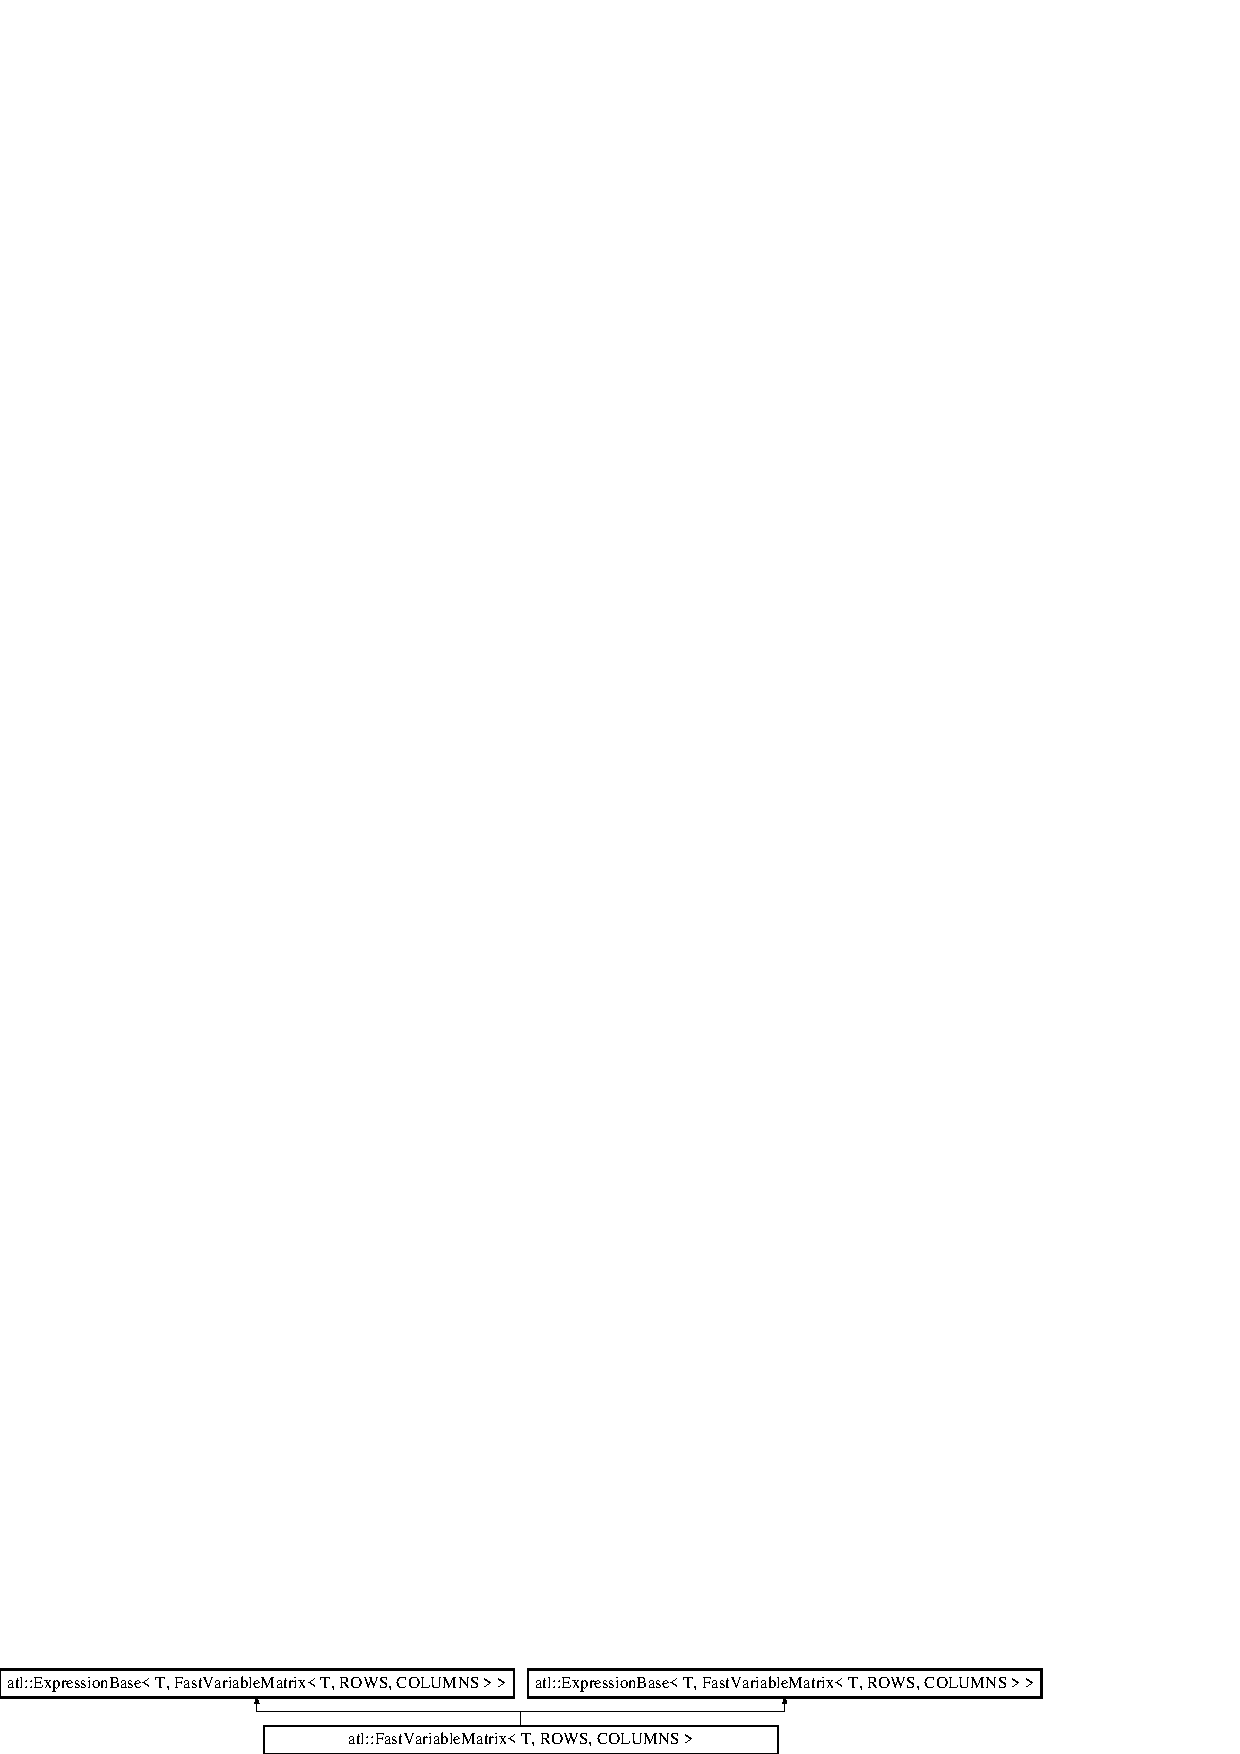
\includegraphics[height=1.320755cm]{structatl_1_1_fast_variable_matrix}
\end{center}
\end{figure}
\subsection*{Public Member Functions}
\begin{DoxyCompactItemize}
\item 
\hypertarget{structatl_1_1_fast_variable_matrix_afa01a66af96313c199bc2aa6e7f0fa74}{{\footnotesize template$<$class A $>$ }\\\hyperlink{structatl_1_1_fast_variable_matrix}{Fast\+Variable\+Matrix} \& {\bfseries operator=} (const \hyperlink{structatl_1_1_expression_base}{Expression\+Base}$<$ T, A $>$ \&exp)}\label{structatl_1_1_fast_variable_matrix_afa01a66af96313c199bc2aa6e7f0fa74}

\item 
\hypertarget{structatl_1_1_fast_variable_matrix_a227d98f3a20e3fcd8cf6a29a5616b5f3}{{\footnotesize template$<$class A $>$ }\\void {\bfseries Assign\+Concurrent} (const \hyperlink{structatl_1_1_expression_base}{Expression\+Base}$<$ T, A $>$ \&exp)}\label{structatl_1_1_fast_variable_matrix_a227d98f3a20e3fcd8cf6a29a5616b5f3}

\item 
\hypertarget{structatl_1_1_fast_variable_matrix_a8af9c6e87cfd817ab521eb4835b7317a}{void {\bfseries Push\+Ids} (typename \hyperlink{structatl_1_1_stack_entry}{atl\+::\+Stack\+Entry}$<$ T $>$\+::vi\+\_\+storage \&ids) const }\label{structatl_1_1_fast_variable_matrix_a8af9c6e87cfd817ab521eb4835b7317a}

\item 
\hypertarget{structatl_1_1_fast_variable_matrix_ab6eedc4ee8dd784c0e72d77ab018439b}{void {\bfseries Push\+Ids} (typename \hyperlink{structatl_1_1_stack_entry}{atl\+::\+Stack\+Entry}$<$ T $>$\+::vi\+\_\+storage \&ids, size\+\_\+t i, size\+\_\+t j=0) const }\label{structatl_1_1_fast_variable_matrix_ab6eedc4ee8dd784c0e72d77ab018439b}

\item 
\hypertarget{structatl_1_1_fast_variable_matrix_acc839a5c65857c92db2334211f396406}{\hyperlink{structatl_1_1_variable}{atl\+::\+Variable}$<$ T $>$ \& {\bfseries operator()} (size\+\_\+t i, size\+\_\+t j=0)}\label{structatl_1_1_fast_variable_matrix_acc839a5c65857c92db2334211f396406}

\item 
\hypertarget{structatl_1_1_fast_variable_matrix_ad6d07f68200eabfc5d08a899ed5374fb}{const \hyperlink{structatl_1_1_variable}{atl\+::\+Variable}$<$ T $>$ \& {\bfseries operator()} (size\+\_\+t i, size\+\_\+t j=0) const }\label{structatl_1_1_fast_variable_matrix_ad6d07f68200eabfc5d08a899ed5374fb}

\item 
\hypertarget{structatl_1_1_fast_variable_matrix_ac1fac676e85f15f4a449daf2743b4ada}{const T {\bfseries Get\+Value} () const }\label{structatl_1_1_fast_variable_matrix_ac1fac676e85f15f4a449daf2743b4ada}

\item 
\hypertarget{structatl_1_1_fast_variable_matrix_afa69688b8746f6df926e7157bba7d1ee}{const T {\bfseries Get\+Value} (size\+\_\+t i, size\+\_\+t j=0) const }\label{structatl_1_1_fast_variable_matrix_afa69688b8746f6df926e7157bba7d1ee}

\item 
\hypertarget{structatl_1_1_fast_variable_matrix_ab4a1d0ed1ab6ca7bbf3e5fd46d99a037}{T {\bfseries Evaluate\+Derivative} (uint32\+\_\+t a) const }\label{structatl_1_1_fast_variable_matrix_ab4a1d0ed1ab6ca7bbf3e5fd46d99a037}

\item 
\hypertarget{structatl_1_1_fast_variable_matrix_a1d9897ad78586dadfa88cecef82b7d65}{T {\bfseries Evaluate\+Derivative} (uint32\+\_\+t a, uint32\+\_\+t b) const }\label{structatl_1_1_fast_variable_matrix_a1d9897ad78586dadfa88cecef82b7d65}

\item 
\hypertarget{structatl_1_1_fast_variable_matrix_a9ed8f0a5e022e4c6422ac477b79ec08e}{T {\bfseries Evaluate\+Derivative} (uint32\+\_\+t x, uint32\+\_\+t y, uint32\+\_\+t z) const }\label{structatl_1_1_fast_variable_matrix_a9ed8f0a5e022e4c6422ac477b79ec08e}

\item 
\hypertarget{structatl_1_1_fast_variable_matrix_a33afd05d2c83c1fb044c7e71c1d0523b}{T {\bfseries Evaluate\+Derivative} (uint32\+\_\+t a, size\+\_\+t i, size\+\_\+t j=0) const }\label{structatl_1_1_fast_variable_matrix_a33afd05d2c83c1fb044c7e71c1d0523b}

\item 
\hypertarget{structatl_1_1_fast_variable_matrix_ade8e35b01619a9f56871d8cf1a9adfec}{T {\bfseries Evaluate\+Derivative} (uint32\+\_\+t a, uint32\+\_\+t b, size\+\_\+t i, size\+\_\+t j=0) const }\label{structatl_1_1_fast_variable_matrix_ade8e35b01619a9f56871d8cf1a9adfec}

\item 
\hypertarget{structatl_1_1_fast_variable_matrix_a9d5a887bfe8d8c73b6ad7c4d70c2a4c7}{T {\bfseries Evaluate\+Derivative} (uint32\+\_\+t x, uint32\+\_\+t y, uint32\+\_\+t z, size\+\_\+t i, size\+\_\+t j=0) const }\label{structatl_1_1_fast_variable_matrix_a9d5a887bfe8d8c73b6ad7c4d70c2a4c7}

\item 
\hypertarget{structatl_1_1_fast_variable_matrix_a3bcd59b609b8006a5c2713df4a5f01d1}{size\+\_\+t {\bfseries Get\+Columns} () const }\label{structatl_1_1_fast_variable_matrix_a3bcd59b609b8006a5c2713df4a5f01d1}

\item 
\hypertarget{structatl_1_1_fast_variable_matrix_a5f4d637293bd81840200afe3cbbb468d}{size\+\_\+t {\bfseries Get\+Rows} () const }\label{structatl_1_1_fast_variable_matrix_a5f4d637293bd81840200afe3cbbb468d}

\item 
\hypertarget{structatl_1_1_fast_variable_matrix_a2d095dbef161ab6e752fe26d36368d30}{bool {\bfseries Is\+Scalar} () const }\label{structatl_1_1_fast_variable_matrix_a2d095dbef161ab6e752fe26d36368d30}

\item 
\hypertarget{structatl_1_1_fast_variable_matrix_afa01a66af96313c199bc2aa6e7f0fa74}{{\footnotesize template$<$class A $>$ }\\\hyperlink{structatl_1_1_fast_variable_matrix}{Fast\+Variable\+Matrix} \& {\bfseries operator=} (const \hyperlink{structatl_1_1_expression_base}{Expression\+Base}$<$ T, A $>$ \&exp)}\label{structatl_1_1_fast_variable_matrix_afa01a66af96313c199bc2aa6e7f0fa74}

\item 
\hypertarget{structatl_1_1_fast_variable_matrix_a227d98f3a20e3fcd8cf6a29a5616b5f3}{{\footnotesize template$<$class A $>$ }\\void {\bfseries Assign\+Concurrent} (const \hyperlink{structatl_1_1_expression_base}{Expression\+Base}$<$ T, A $>$ \&exp)}\label{structatl_1_1_fast_variable_matrix_a227d98f3a20e3fcd8cf6a29a5616b5f3}

\item 
\hypertarget{structatl_1_1_fast_variable_matrix_a8af9c6e87cfd817ab521eb4835b7317a}{void {\bfseries Push\+Ids} (typename \hyperlink{structatl_1_1_stack_entry}{atl\+::\+Stack\+Entry}$<$ T $>$\+::vi\+\_\+storage \&ids) const }\label{structatl_1_1_fast_variable_matrix_a8af9c6e87cfd817ab521eb4835b7317a}

\item 
\hypertarget{structatl_1_1_fast_variable_matrix_ab6eedc4ee8dd784c0e72d77ab018439b}{void {\bfseries Push\+Ids} (typename \hyperlink{structatl_1_1_stack_entry}{atl\+::\+Stack\+Entry}$<$ T $>$\+::vi\+\_\+storage \&ids, size\+\_\+t i, size\+\_\+t j=0) const }\label{structatl_1_1_fast_variable_matrix_ab6eedc4ee8dd784c0e72d77ab018439b}

\item 
\hypertarget{structatl_1_1_fast_variable_matrix_acc839a5c65857c92db2334211f396406}{\hyperlink{structatl_1_1_variable}{atl\+::\+Variable}$<$ T $>$ \& {\bfseries operator()} (size\+\_\+t i, size\+\_\+t j=0)}\label{structatl_1_1_fast_variable_matrix_acc839a5c65857c92db2334211f396406}

\item 
\hypertarget{structatl_1_1_fast_variable_matrix_ad6d07f68200eabfc5d08a899ed5374fb}{const \hyperlink{structatl_1_1_variable}{atl\+::\+Variable}$<$ T $>$ \& {\bfseries operator()} (size\+\_\+t i, size\+\_\+t j=0) const }\label{structatl_1_1_fast_variable_matrix_ad6d07f68200eabfc5d08a899ed5374fb}

\item 
\hypertarget{structatl_1_1_fast_variable_matrix_ac1fac676e85f15f4a449daf2743b4ada}{const T {\bfseries Get\+Value} () const }\label{structatl_1_1_fast_variable_matrix_ac1fac676e85f15f4a449daf2743b4ada}

\item 
\hypertarget{structatl_1_1_fast_variable_matrix_afa69688b8746f6df926e7157bba7d1ee}{const T {\bfseries Get\+Value} (size\+\_\+t i, size\+\_\+t j=0) const }\label{structatl_1_1_fast_variable_matrix_afa69688b8746f6df926e7157bba7d1ee}

\item 
\hypertarget{structatl_1_1_fast_variable_matrix_ab4a1d0ed1ab6ca7bbf3e5fd46d99a037}{T {\bfseries Evaluate\+Derivative} (uint32\+\_\+t a) const }\label{structatl_1_1_fast_variable_matrix_ab4a1d0ed1ab6ca7bbf3e5fd46d99a037}

\item 
\hypertarget{structatl_1_1_fast_variable_matrix_a1d9897ad78586dadfa88cecef82b7d65}{T {\bfseries Evaluate\+Derivative} (uint32\+\_\+t a, uint32\+\_\+t b) const }\label{structatl_1_1_fast_variable_matrix_a1d9897ad78586dadfa88cecef82b7d65}

\item 
\hypertarget{structatl_1_1_fast_variable_matrix_a9ed8f0a5e022e4c6422ac477b79ec08e}{T {\bfseries Evaluate\+Derivative} (uint32\+\_\+t x, uint32\+\_\+t y, uint32\+\_\+t z) const }\label{structatl_1_1_fast_variable_matrix_a9ed8f0a5e022e4c6422ac477b79ec08e}

\item 
\hypertarget{structatl_1_1_fast_variable_matrix_a33afd05d2c83c1fb044c7e71c1d0523b}{T {\bfseries Evaluate\+Derivative} (uint32\+\_\+t a, size\+\_\+t i, size\+\_\+t j=0) const }\label{structatl_1_1_fast_variable_matrix_a33afd05d2c83c1fb044c7e71c1d0523b}

\item 
\hypertarget{structatl_1_1_fast_variable_matrix_ade8e35b01619a9f56871d8cf1a9adfec}{T {\bfseries Evaluate\+Derivative} (uint32\+\_\+t a, uint32\+\_\+t b, size\+\_\+t i, size\+\_\+t j=0) const }\label{structatl_1_1_fast_variable_matrix_ade8e35b01619a9f56871d8cf1a9adfec}

\item 
\hypertarget{structatl_1_1_fast_variable_matrix_a9d5a887bfe8d8c73b6ad7c4d70c2a4c7}{T {\bfseries Evaluate\+Derivative} (uint32\+\_\+t x, uint32\+\_\+t y, uint32\+\_\+t z, size\+\_\+t i, size\+\_\+t j=0) const }\label{structatl_1_1_fast_variable_matrix_a9d5a887bfe8d8c73b6ad7c4d70c2a4c7}

\item 
\hypertarget{structatl_1_1_fast_variable_matrix_a3bcd59b609b8006a5c2713df4a5f01d1}{size\+\_\+t {\bfseries Get\+Columns} () const }\label{structatl_1_1_fast_variable_matrix_a3bcd59b609b8006a5c2713df4a5f01d1}

\item 
\hypertarget{structatl_1_1_fast_variable_matrix_a5f4d637293bd81840200afe3cbbb468d}{size\+\_\+t {\bfseries Get\+Rows} () const }\label{structatl_1_1_fast_variable_matrix_a5f4d637293bd81840200afe3cbbb468d}

\item 
\hypertarget{structatl_1_1_fast_variable_matrix_a2d095dbef161ab6e752fe26d36368d30}{bool {\bfseries Is\+Scalar} () const }\label{structatl_1_1_fast_variable_matrix_a2d095dbef161ab6e752fe26d36368d30}

\item 
\hypertarget{structatl_1_1_fast_variable_matrix_a541d290c8e65a193dfb33cd980378df9}{const std\+::string {\bfseries To\+Expression\+Template\+String} () const }\label{structatl_1_1_fast_variable_matrix_a541d290c8e65a193dfb33cd980378df9}

\end{DoxyCompactItemize}
\subsection*{Public Attributes}
\begin{DoxyCompactItemize}
\item 
\hypertarget{structatl_1_1_fast_variable_matrix_a6eda2199e053d42508cfd95b30550d13}{size\+\_\+t {\bfseries rows} = R\+O\+W\+S}\label{structatl_1_1_fast_variable_matrix_a6eda2199e053d42508cfd95b30550d13}

\item 
\hypertarget{structatl_1_1_fast_variable_matrix_af2073a0de77f4b34465ecc697893225a}{size\+\_\+t {\bfseries columns} = C\+O\+L\+U\+M\+N\+S}\label{structatl_1_1_fast_variable_matrix_af2073a0de77f4b34465ecc697893225a}

\item 
\hypertarget{structatl_1_1_fast_variable_matrix_acaf869666ab9d0e81443c68a458b9489}{\hyperlink{structatl_1_1_variable}{atl\+::\+Variable}$<$ T $>$ {\bfseries data\+\_\+m} \mbox{[}R\+O\+W\+S $\ast$C\+O\+L\+U\+M\+N\+S\mbox{]}}\label{structatl_1_1_fast_variable_matrix_acaf869666ab9d0e81443c68a458b9489}

\end{DoxyCompactItemize}


The documentation for this struct was generated from the following file\+:\begin{DoxyCompactItemize}
\item 
A\+T\+L2/Matrix.\+hpp\end{DoxyCompactItemize}

\hypertarget{classflat__map}{\section{flat\+\_\+map$<$ Key, T $>$ Class Template Reference}
\label{classflat__map}\index{flat\+\_\+map$<$ Key, T $>$@{flat\+\_\+map$<$ Key, T $>$}}
}
\subsection*{Public Types}
\begin{DoxyCompactItemize}
\item 
\hypertarget{classflat__map_a6581ef62bd21bb226dfe517c3ed43b5a}{typedef std\+::pair$<$ Key, T $>$ {\bfseries value\+\_\+type}}\label{classflat__map_a6581ef62bd21bb226dfe517c3ed43b5a}

\item 
\hypertarget{classflat__map_a7e95e5b3dda48e5c2474ca6b909d2677}{typedef Key {\bfseries key\+\_\+type}}\label{classflat__map_a7e95e5b3dda48e5c2474ca6b909d2677}

\item 
\hypertarget{classflat__map_a7613e7e076835aa5cf82b080f43bb0b5}{typedef T {\bfseries mapped\+\_\+type}}\label{classflat__map_a7613e7e076835aa5cf82b080f43bb0b5}

\item 
\hypertarget{classflat__map_ab4a6ac010ab97689b3a62818e2a6614a}{typedef std\+::vector\\*
$<$ value\+\_\+type $>$\+::iterator {\bfseries iterator}}\label{classflat__map_ab4a6ac010ab97689b3a62818e2a6614a}

\item 
\hypertarget{classflat__map_a933a888ad3685b983832290d386433bb}{typedef std\+::vector\\*
$<$ value\+\_\+type $>$\+::const\+\_\+iterator {\bfseries const\+\_\+iterator}}\label{classflat__map_a933a888ad3685b983832290d386433bb}

\item 
\hypertarget{classflat__map_aa5e77dd653cc21aa6c61d256cc028d27}{typedef std\+::vector\\*
$<$ value\+\_\+type $>$\\*
\+::reverse\+\_\+iterator {\bfseries reverse\+\_\+iterator}}\label{classflat__map_aa5e77dd653cc21aa6c61d256cc028d27}

\item 
\hypertarget{classflat__map_a59a3e7bca67921951ba0e4cc60ab911b}{typedef std\+::vector\\*
$<$ value\+\_\+type $>$\\*
\+::const\+\_\+reverse\+\_\+iterator {\bfseries const\+\_\+reverse\+\_\+iterator}}\label{classflat__map_a59a3e7bca67921951ba0e4cc60ab911b}

\end{DoxyCompactItemize}
\subsection*{Public Member Functions}
\begin{DoxyCompactItemize}
\item 
\hypertarget{classflat__map_abd94965cca27bf799dd21e99a224aa78}{{\bfseries flat\+\_\+map} (std\+::size\+\_\+t n=0)}\label{classflat__map_abd94965cca27bf799dd21e99a224aa78}

\item 
\hypertarget{classflat__map_a69b4fb77d523f0667509d272f6176e8a}{std\+::pair$<$ iterator, bool $>$ {\bfseries insert} (const value\+\_\+type \&value)}\label{classflat__map_a69b4fb77d523f0667509d272f6176e8a}

\item 
\hypertarget{classflat__map_af836dd7b5a1c3fabb932ea38fc50fe37}{T \& {\bfseries operator\mbox{[}$\,$\mbox{]}} (const Key \&key)}\label{classflat__map_af836dd7b5a1c3fabb932ea38fc50fe37}

\item 
\hypertarget{classflat__map_aa272d0f4b7e738f18589f1dc7e0e5bca}{void {\bfseries swap} (\hyperlink{classflat__map}{flat\+\_\+map} \&m)}\label{classflat__map_aa272d0f4b7e738f18589f1dc7e0e5bca}

\item 
\hypertarget{classflat__map_a3c10f97ddf0408caafeb34d3a65cc594}{iterator {\bfseries find} (const Key \&key)}\label{classflat__map_a3c10f97ddf0408caafeb34d3a65cc594}

\item 
\hypertarget{classflat__map_a5590f1396408427930a5b8dd400668fb}{const\+\_\+iterator {\bfseries find} (const Key \&key) const }\label{classflat__map_a5590f1396408427930a5b8dd400668fb}

\item 
\hypertarget{classflat__map_a25634923ff2cb3a82351ec2ea7149c5b}{void {\bfseries erase} (const Key \&key)}\label{classflat__map_a25634923ff2cb3a82351ec2ea7149c5b}

\item 
\hypertarget{classflat__map_a9390ff85c2ed502aa78274c1e890eec1}{void {\bfseries clear} ()}\label{classflat__map_a9390ff85c2ed502aa78274c1e890eec1}

\item 
\hypertarget{classflat__map_a152ea87db1ff83c682ac857196d9bc9e}{void {\bfseries reset} ()}\label{classflat__map_a152ea87db1ff83c682ac857196d9bc9e}

\item 
\hypertarget{classflat__map_a441b623ecb19e142a5ddad11c87c6010}{bool {\bfseries empty} () const }\label{classflat__map_a441b623ecb19e142a5ddad11c87c6010}

\item 
\hypertarget{classflat__map_a9f3e1a23bbc5c1101f301e76c503d070}{std\+::size\+\_\+t {\bfseries size} () const }\label{classflat__map_a9f3e1a23bbc5c1101f301e76c503d070}

\item 
\hypertarget{classflat__map_a7301695b0a7a9fdd07d258fcc6a4b205}{iterator {\bfseries begin} ()}\label{classflat__map_a7301695b0a7a9fdd07d258fcc6a4b205}

\item 
\hypertarget{classflat__map_a41b9475e5165f1542cdf9fc193a72ba8}{iterator {\bfseries end} ()}\label{classflat__map_a41b9475e5165f1542cdf9fc193a72ba8}

\item 
\hypertarget{classflat__map_a182181c6576aefbddc0dd58b9a3772e2}{const\+\_\+iterator {\bfseries begin} () const }\label{classflat__map_a182181c6576aefbddc0dd58b9a3772e2}

\item 
\hypertarget{classflat__map_adc262dfd937bf15806a82165241de03d}{const\+\_\+iterator {\bfseries end} () const }\label{classflat__map_adc262dfd937bf15806a82165241de03d}

\item 
\hypertarget{classflat__map_aa80ae3434ed2b0901fcbaff2091a93ab}{reverse\+\_\+iterator {\bfseries rbegin} ()}\label{classflat__map_aa80ae3434ed2b0901fcbaff2091a93ab}

\item 
\hypertarget{classflat__map_a4f45c455f9b94c174d495b4e0b20e450}{reverse\+\_\+iterator {\bfseries rend} ()}\label{classflat__map_a4f45c455f9b94c174d495b4e0b20e450}

\item 
\hypertarget{classflat__map_abd5583f53e0610b764731e5835be7fbe}{const\+\_\+reverse\+\_\+iterator {\bfseries rbegin} () const }\label{classflat__map_abd5583f53e0610b764731e5835be7fbe}

\item 
\hypertarget{classflat__map_a1b2cb77af4089b3d35dcda7e579f2d26}{const\+\_\+reverse\+\_\+iterator {\bfseries rend} () const }\label{classflat__map_a1b2cb77af4089b3d35dcda7e579f2d26}

\item 
\hypertarget{classflat__map_a0c1b4fa6cdca305eefd5a9c5091a4203}{std\+::vector$<$ value\+\_\+type $>$ \& {\bfseries data} ()}\label{classflat__map_a0c1b4fa6cdca305eefd5a9c5091a4203}

\item 
\hypertarget{classflat__map_a1473a25884b4fdc46abae379ce7110e9}{const std\+::vector$<$ value\+\_\+type $>$ \& {\bfseries data} () const }\label{classflat__map_a1473a25884b4fdc46abae379ce7110e9}

\end{DoxyCompactItemize}


The documentation for this class was generated from the following file\+:\begin{DoxyCompactItemize}
\item 
Utilities/flat\+\_\+map.\+hpp\end{DoxyCompactItemize}

\hypertarget{classflat__set}{\section{flat\+\_\+set$<$ T, Compare, Allocator $>$ Class Template Reference}
\label{classflat__set}\index{flat\+\_\+set$<$ T, Compare, Allocator $>$@{flat\+\_\+set$<$ T, Compare, Allocator $>$}}
}
\subsection*{Public Types}
\begin{DoxyCompactItemize}
\item 
\hypertarget{classflat__set_a32ab9f38f230df82e9c3ca4b0e833419}{typedef std\+::vector$<$ T $>$\+::iterator {\bfseries iterator}}\label{classflat__set_a32ab9f38f230df82e9c3ca4b0e833419}

\item 
\hypertarget{classflat__set_a2bbb78ab23ff89845c14ecb418485d47}{typedef std\+::vector$<$ T $>$\\*
\+::const\+\_\+iterator {\bfseries const\+\_\+iterator}}\label{classflat__set_a2bbb78ab23ff89845c14ecb418485d47}

\item 
\hypertarget{classflat__set_acd5fb908d5f63906824e8dc85ad948bb}{typedef std\+::vector$<$ T $>$\\*
\+::reverse\+\_\+iterator {\bfseries reverse\+\_\+iterator}}\label{classflat__set_acd5fb908d5f63906824e8dc85ad948bb}

\item 
\hypertarget{classflat__set_a2489a867ea00fbfff1c8ddf510d2d75a}{typedef std\+::vector$<$ T $>$\\*
\+::const\+\_\+reverse\+\_\+iterator {\bfseries const\+\_\+reverse\+\_\+iterator}}\label{classflat__set_a2489a867ea00fbfff1c8ddf510d2d75a}

\end{DoxyCompactItemize}
\subsection*{Public Member Functions}
\begin{DoxyCompactItemize}
\item 
\hypertarget{classflat__set_a142169ea5c7b6b049370394cfed3fe65}{{\bfseries flat\+\_\+set} (const Compare \&c=Compare())}\label{classflat__set_a142169ea5c7b6b049370394cfed3fe65}

\item 
\hypertarget{classflat__set_ad3f86af87854578d171995c723ffbc14}{{\footnotesize template$<$class Input\+Iterator $>$ }\\{\bfseries flat\+\_\+set} (Input\+Iterator first, Input\+Iterator last, const Compare \&c=Compare())}\label{classflat__set_ad3f86af87854578d171995c723ffbc14}

\item 
\hypertarget{classflat__set_ae5ca211c594636479b3c0d2ffcd24a56}{iterator {\bfseries erase} (const T \&t)}\label{classflat__set_ae5ca211c594636479b3c0d2ffcd24a56}

\item 
\hypertarget{classflat__set_afe5aa132ec1d9ac7fb3fa9b95e367bae}{iterator {\bfseries insert} (const T \&t)}\label{classflat__set_afe5aa132ec1d9ac7fb3fa9b95e367bae}

\item 
\hypertarget{classflat__set_a086669072cb6717f2b221803d4f22eb0}{void {\bfseries insert} (const iterator \&first, const iterator \&last)}\label{classflat__set_a086669072cb6717f2b221803d4f22eb0}

\item 
\hypertarget{classflat__set_a46c3cf5c64ff20392c0a2d2781f007b8}{const\+\_\+iterator {\bfseries find} (const T \&t) const }\label{classflat__set_a46c3cf5c64ff20392c0a2d2781f007b8}

\item 
\hypertarget{classflat__set_a368e5bc9b1b3a0f819c75919af9c64c7}{iterator {\bfseries find} (const T \&t)}\label{classflat__set_a368e5bc9b1b3a0f819c75919af9c64c7}

\item 
\hypertarget{classflat__set_a439bcd47ee6d8e3219094071519be91a}{iterator {\bfseries begin} ()}\label{classflat__set_a439bcd47ee6d8e3219094071519be91a}

\item 
\hypertarget{classflat__set_a92caeed16ea8d949a1ff7ba55854333f}{iterator {\bfseries end} ()}\label{classflat__set_a92caeed16ea8d949a1ff7ba55854333f}

\item 
\hypertarget{classflat__set_af86fd56851cc79707b8047f41515e6e5}{const\+\_\+iterator {\bfseries begin} () const }\label{classflat__set_af86fd56851cc79707b8047f41515e6e5}

\item 
\hypertarget{classflat__set_adfb11e89187e89ad311e757483434e11}{const\+\_\+iterator {\bfseries end} () const }\label{classflat__set_adfb11e89187e89ad311e757483434e11}

\item 
\hypertarget{classflat__set_a3f332e9e1a8230e39a889fb6767f5c3a}{reverse\+\_\+iterator {\bfseries rbegin} ()}\label{classflat__set_a3f332e9e1a8230e39a889fb6767f5c3a}

\item 
\hypertarget{classflat__set_a31c60bdf0b34dddf9320823989346100}{reverse\+\_\+iterator {\bfseries rend} ()}\label{classflat__set_a31c60bdf0b34dddf9320823989346100}

\item 
\hypertarget{classflat__set_a3cd547467d9e3e7d5b9c090f11416ea5}{const\+\_\+reverse\+\_\+iterator {\bfseries rbegin} () const }\label{classflat__set_a3cd547467d9e3e7d5b9c090f11416ea5}

\item 
\hypertarget{classflat__set_a657c70613a6df781ddfb7acaf5accab3}{const\+\_\+reverse\+\_\+iterator {\bfseries rend} () const }\label{classflat__set_a657c70613a6df781ddfb7acaf5accab3}

\item 
\hypertarget{classflat__set_a995982d56034fcfbe43d9d3e9453849d}{size\+\_\+t {\bfseries size} () const }\label{classflat__set_a995982d56034fcfbe43d9d3e9453849d}

\item 
\hypertarget{classflat__set_a9056b7f67544da53af05f1cf201df143}{void {\bfseries reserve} (size\+\_\+t size)}\label{classflat__set_a9056b7f67544da53af05f1cf201df143}

\item 
\hypertarget{classflat__set_a2b6cf8460b0962079651453fb40e57e8}{std\+::vector$<$ T, Allocator $>$ \& {\bfseries data} ()}\label{classflat__set_a2b6cf8460b0962079651453fb40e57e8}

\item 
\hypertarget{classflat__set_a822dbda7e154f6c74a465178561f2a17}{bool {\bfseries contains} (const T \&t)}\label{classflat__set_a822dbda7e154f6c74a465178561f2a17}

\item 
\hypertarget{classflat__set_ad86c71e5a1cda8a6381d908d1e4687eb}{void {\bfseries clear} ()}\label{classflat__set_ad86c71e5a1cda8a6381d908d1e4687eb}

\item 
\hypertarget{classflat__set_a86dfac5d359fbd179b144b79da3fb415}{void {\bfseries clear\+\_\+no\+\_\+resize} ()}\label{classflat__set_a86dfac5d359fbd179b144b79da3fb415}

\end{DoxyCompactItemize}


The documentation for this class was generated from the following file\+:\begin{DoxyCompactItemize}
\item 
Utilities/flat\+\_\+set.\+hpp\end{DoxyCompactItemize}

\hypertarget{structatl_1_1_floor}{\section{atl\+:\+:Floor$<$ R\+E\+A\+L\+\_\+\+T, E\+X\+P\+R $>$ Struct Template Reference}
\label{structatl_1_1_floor}\index{atl\+::\+Floor$<$ R\+E\+A\+L\+\_\+\+T, E\+X\+P\+R $>$@{atl\+::\+Floor$<$ R\+E\+A\+L\+\_\+\+T, E\+X\+P\+R $>$}}
}


{\ttfamily \#include $<$Floor.\+hpp$>$}

Inheritance diagram for atl\+:\+:Floor$<$ R\+E\+A\+L\+\_\+\+T, E\+X\+P\+R $>$\+:\begin{figure}[H]
\begin{center}
\leavevmode
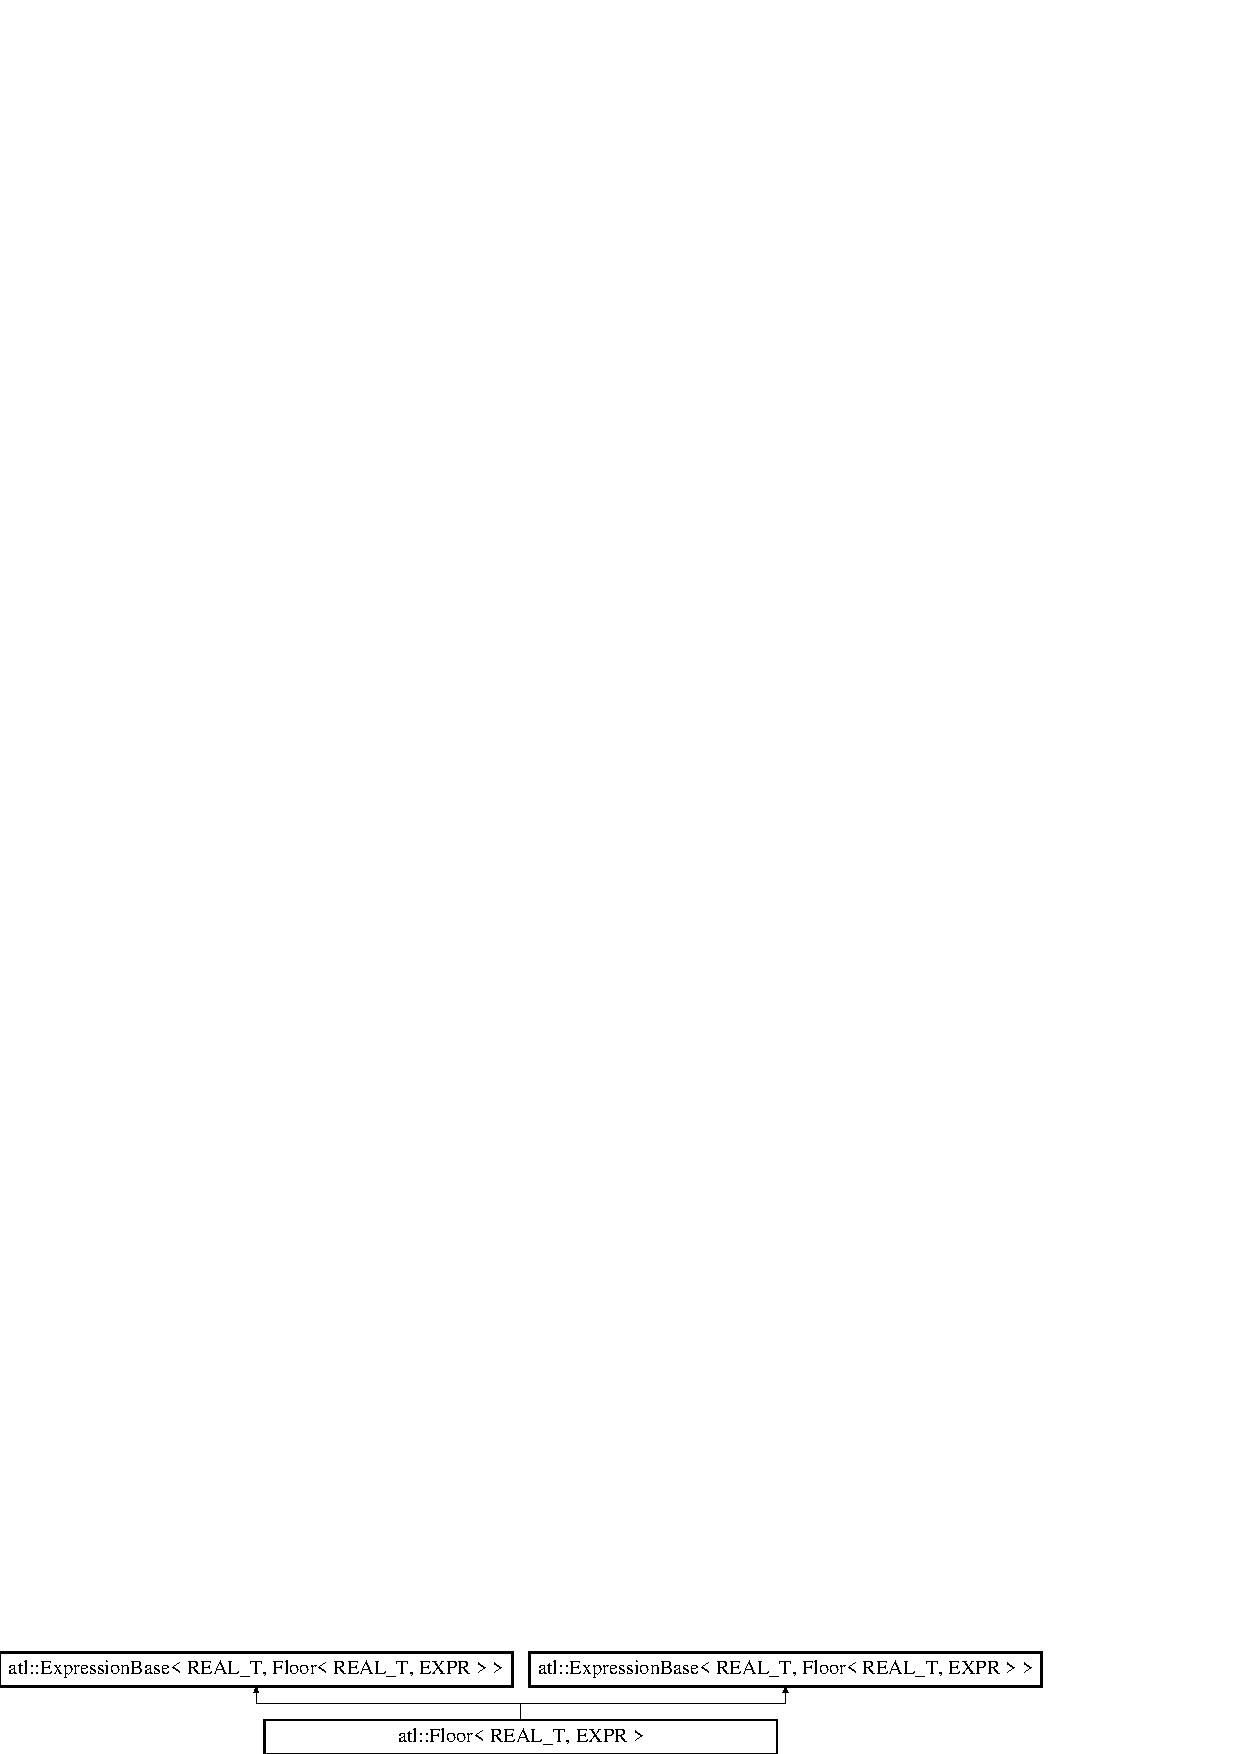
\includegraphics[height=1.600000cm]{structatl_1_1_floor}
\end{center}
\end{figure}
\subsection*{Public Types}
\begin{DoxyCompactItemize}
\item 
\hypertarget{structatl_1_1_floor_a993fa1a6710cdba80b7b63774f837452}{typedef R\+E\+A\+L\+\_\+\+T {\bfseries B\+A\+S\+E\+\_\+\+T\+Y\+P\+E}}\label{structatl_1_1_floor_a993fa1a6710cdba80b7b63774f837452}

\item 
\hypertarget{structatl_1_1_floor_a993fa1a6710cdba80b7b63774f837452}{typedef R\+E\+A\+L\+\_\+\+T {\bfseries B\+A\+S\+E\+\_\+\+T\+Y\+P\+E}}\label{structatl_1_1_floor_a993fa1a6710cdba80b7b63774f837452}

\end{DoxyCompactItemize}
\subsection*{Public Member Functions}
\begin{DoxyCompactItemize}
\item 
\hypertarget{structatl_1_1_floor_aef10e331b5a8dfd105d4625834805ed5}{{\bfseries Floor} (const \hyperlink{structatl_1_1_expression_base}{Expression\+Base}$<$ R\+E\+A\+L\+\_\+\+T, E\+X\+P\+R $>$ \&a)}\label{structatl_1_1_floor_aef10e331b5a8dfd105d4625834805ed5}

\item 
\hypertarget{structatl_1_1_floor_a0ba9ceb76ef311d1e744fd33ab5e26a0}{const R\+E\+A\+L\+\_\+\+T {\bfseries Get\+Value} () const }\label{structatl_1_1_floor_a0ba9ceb76ef311d1e744fd33ab5e26a0}

\item 
\hypertarget{structatl_1_1_floor_abb51bf2e1df3e1aaa608e2fe1d8f4b6c}{const R\+E\+A\+L\+\_\+\+T {\bfseries Get\+Value} (size\+\_\+t i, size\+\_\+t j=0) const }\label{structatl_1_1_floor_abb51bf2e1df3e1aaa608e2fe1d8f4b6c}

\item 
\hypertarget{structatl_1_1_floor_a00a63079149c6ba771d85003063555a1}{void {\bfseries Push\+Ids} (typename \hyperlink{structatl_1_1_stack_entry}{atl\+::\+Stack\+Entry}$<$ R\+E\+A\+L\+\_\+\+T $>$\+::vi\+\_\+storage \&ids) const }\label{structatl_1_1_floor_a00a63079149c6ba771d85003063555a1}

\item 
\hypertarget{structatl_1_1_floor_a163741875a38d29e0f8bae05690ecee2}{void {\bfseries Push\+Ids} (typename \hyperlink{structatl_1_1_stack_entry}{atl\+::\+Stack\+Entry}$<$ R\+E\+A\+L\+\_\+\+T $>$\+::vi\+\_\+storage \&ids, size\+\_\+t i, size\+\_\+t j=0) const }\label{structatl_1_1_floor_a163741875a38d29e0f8bae05690ecee2}

\item 
\hypertarget{structatl_1_1_floor_a57802c11d13cc65b6b4c5277c166fcec}{const R\+E\+A\+L\+\_\+\+T {\bfseries Evaluate\+Derivative} (uint32\+\_\+t id) const }\label{structatl_1_1_floor_a57802c11d13cc65b6b4c5277c166fcec}

\item 
\hypertarget{structatl_1_1_floor_afd7244e0957f110672b9f796df384cd2}{R\+E\+A\+L\+\_\+\+T {\bfseries Evaluate\+Derivative} (uint32\+\_\+t a, uint32\+\_\+t b) const }\label{structatl_1_1_floor_afd7244e0957f110672b9f796df384cd2}

\item 
\hypertarget{structatl_1_1_floor_a7819c933ee40dfdda197cf0a84815d3f}{R\+E\+A\+L\+\_\+\+T {\bfseries Evaluate\+Derivative} (uint32\+\_\+t x, uint32\+\_\+t y, uint32\+\_\+t z) const }\label{structatl_1_1_floor_a7819c933ee40dfdda197cf0a84815d3f}

\item 
\hypertarget{structatl_1_1_floor_a7b1680974460bb030aad835bd78a0e15}{const R\+E\+A\+L\+\_\+\+T {\bfseries Evaluate\+Derivative} (uint32\+\_\+t id, size\+\_\+t i, size\+\_\+t j=0) const }\label{structatl_1_1_floor_a7b1680974460bb030aad835bd78a0e15}

\item 
\hypertarget{structatl_1_1_floor_a6116d4e32adb9d748bdf346f1e6df82a}{R\+E\+A\+L\+\_\+\+T {\bfseries Evaluate\+Derivative} (uint32\+\_\+t a, uint32\+\_\+t b, size\+\_\+t i, size\+\_\+t j=0) const }\label{structatl_1_1_floor_a6116d4e32adb9d748bdf346f1e6df82a}

\item 
\hypertarget{structatl_1_1_floor_a4f6cf89a00ef56ca69c487891f62edb9}{R\+E\+A\+L\+\_\+\+T {\bfseries Evaluate\+Derivative} (uint32\+\_\+t x, uint32\+\_\+t y, uint32\+\_\+t z, size\+\_\+t i, size\+\_\+t j=0) const }\label{structatl_1_1_floor_a4f6cf89a00ef56ca69c487891f62edb9}

\item 
\hypertarget{structatl_1_1_floor_aed881508e0865ed92d3e7106ece635c3}{size\+\_\+t {\bfseries Get\+Columns} () const }\label{structatl_1_1_floor_aed881508e0865ed92d3e7106ece635c3}

\item 
\hypertarget{structatl_1_1_floor_adfa56c6c6bafc644dc6c5379b7eee93f}{size\+\_\+t {\bfseries Get\+Rows} () const }\label{structatl_1_1_floor_adfa56c6c6bafc644dc6c5379b7eee93f}

\item 
\hypertarget{structatl_1_1_floor_ac16d9a293b83387f2250c3d5c8355bea}{bool {\bfseries Is\+Scalar} () const }\label{structatl_1_1_floor_ac16d9a293b83387f2250c3d5c8355bea}

\item 
\hyperlink{structatl_1_1_floor_aef10e331b5a8dfd105d4625834805ed5}{Floor} (const \hyperlink{structatl_1_1_expression_base}{Expression\+Base}$<$ R\+E\+A\+L\+\_\+\+T, E\+X\+P\+R $>$ \&a)
\item 
const R\+E\+A\+L\+\_\+\+T \hyperlink{structatl_1_1_floor_a0ba9ceb76ef311d1e744fd33ab5e26a0}{Get\+Value} () const 
\item 
const R\+E\+A\+L\+\_\+\+T \hyperlink{structatl_1_1_floor_abb51bf2e1df3e1aaa608e2fe1d8f4b6c}{Get\+Value} (size\+\_\+t i, size\+\_\+t j=0) const 
\item 
bool \hyperlink{structatl_1_1_floor_ae166074543f85f765c5de9596b39eff8}{Is\+Nonlinear} () const 
\item 
void \hyperlink{structatl_1_1_floor_a00a63079149c6ba771d85003063555a1}{Push\+Ids} (typename \hyperlink{structatl_1_1_stack_entry}{atl\+::\+Stack\+Entry}$<$ R\+E\+A\+L\+\_\+\+T $>$\+::vi\+\_\+storage \&ids) const 
\item 
void \hyperlink{structatl_1_1_floor_a163741875a38d29e0f8bae05690ecee2}{Push\+Ids} (typename \hyperlink{structatl_1_1_stack_entry}{atl\+::\+Stack\+Entry}$<$ R\+E\+A\+L\+\_\+\+T $>$\+::vi\+\_\+storage \&ids, size\+\_\+t i, size\+\_\+t j=0) const 
\item 
const R\+E\+A\+L\+\_\+\+T \hyperlink{structatl_1_1_floor_a57802c11d13cc65b6b4c5277c166fcec}{Evaluate\+Derivative} (uint32\+\_\+t id) const 
\item 
R\+E\+A\+L\+\_\+\+T \hyperlink{structatl_1_1_floor_afd7244e0957f110672b9f796df384cd2}{Evaluate\+Derivative} (uint32\+\_\+t a, uint32\+\_\+t b) const 
\item 
R\+E\+A\+L\+\_\+\+T \hyperlink{structatl_1_1_floor_a7819c933ee40dfdda197cf0a84815d3f}{Evaluate\+Derivative} (uint32\+\_\+t x, uint32\+\_\+t y, uint32\+\_\+t z) const 
\item 
const R\+E\+A\+L\+\_\+\+T \hyperlink{structatl_1_1_floor_a7b1680974460bb030aad835bd78a0e15}{Evaluate\+Derivative} (uint32\+\_\+t id, size\+\_\+t i, size\+\_\+t j=0) const 
\item 
R\+E\+A\+L\+\_\+\+T \hyperlink{structatl_1_1_floor_a6116d4e32adb9d748bdf346f1e6df82a}{Evaluate\+Derivative} (uint32\+\_\+t a, uint32\+\_\+t b, size\+\_\+t i, size\+\_\+t j=0) const 
\item 
R\+E\+A\+L\+\_\+\+T \hyperlink{structatl_1_1_floor_a4f6cf89a00ef56ca69c487891f62edb9}{Evaluate\+Derivative} (uint32\+\_\+t x, uint32\+\_\+t y, uint32\+\_\+t z, size\+\_\+t i, size\+\_\+t j=0) const 
\item 
size\+\_\+t \hyperlink{structatl_1_1_floor_aed881508e0865ed92d3e7106ece635c3}{Get\+Columns} () const 
\item 
size\+\_\+t \hyperlink{structatl_1_1_floor_adfa56c6c6bafc644dc6c5379b7eee93f}{Get\+Rows} () const 
\item 
bool \hyperlink{structatl_1_1_floor_ac16d9a293b83387f2250c3d5c8355bea}{Is\+Scalar} () const 
\item 
const std\+::string \hyperlink{structatl_1_1_floor_a285e4e518da19e29e0bcfe72de5c6f47}{To\+Expression\+Template\+String} () const 
\end{DoxyCompactItemize}
\subsection*{Public Attributes}
\begin{DoxyCompactItemize}
\item 
\hypertarget{structatl_1_1_floor_af1657ef328c1039556c17e574bf98350}{const E\+X\+P\+R \& {\bfseries expr\+\_\+m}}\label{structatl_1_1_floor_af1657ef328c1039556c17e574bf98350}

\end{DoxyCompactItemize}


\subsection{Detailed Description}
\subsubsection*{template$<$class R\+E\+A\+L\+\_\+\+T, class E\+X\+P\+R$>$struct atl\+::\+Floor$<$ R\+E\+A\+L\+\_\+\+T, E\+X\+P\+R $>$}

Expression template to handle cosine for variable or container expressions.

$ \floor f(x,y) $

or

$ \floor f_{i,j}(x,y) $

This is not differentiable and calls to the derivative member functions result in 0. 

\subsection{Constructor \& Destructor Documentation}
\hypertarget{structatl_1_1_floor_aef10e331b5a8dfd105d4625834805ed5}{\index{atl\+::\+Floor@{atl\+::\+Floor}!Floor@{Floor}}
\index{Floor@{Floor}!atl\+::\+Floor@{atl\+::\+Floor}}
\subsubsection[{Floor}]{\setlength{\rightskip}{0pt plus 5cm}template$<$class R\+E\+A\+L\+\_\+\+T , class E\+X\+P\+R $>$ {\bf atl\+::\+Floor}$<$ R\+E\+A\+L\+\_\+\+T, E\+X\+P\+R $>$\+::{\bf Floor} (
\begin{DoxyParamCaption}
\item[{const {\bf Expression\+Base}$<$ R\+E\+A\+L\+\_\+\+T, E\+X\+P\+R $>$ \&}]{a}
\end{DoxyParamCaption}
)\hspace{0.3cm}{\ttfamily [inline]}}}\label{structatl_1_1_floor_aef10e331b5a8dfd105d4625834805ed5}
Constructor


\begin{DoxyParams}{Parameters}
{\em a} & \\
\hline
\end{DoxyParams}


\subsection{Member Function Documentation}
\hypertarget{structatl_1_1_floor_a57802c11d13cc65b6b4c5277c166fcec}{\index{atl\+::\+Floor@{atl\+::\+Floor}!Evaluate\+Derivative@{Evaluate\+Derivative}}
\index{Evaluate\+Derivative@{Evaluate\+Derivative}!atl\+::\+Floor@{atl\+::\+Floor}}
\subsubsection[{Evaluate\+Derivative}]{\setlength{\rightskip}{0pt plus 5cm}template$<$class R\+E\+A\+L\+\_\+\+T , class E\+X\+P\+R $>$ const R\+E\+A\+L\+\_\+\+T {\bf atl\+::\+Floor}$<$ R\+E\+A\+L\+\_\+\+T, E\+X\+P\+R $>$\+::Evaluate\+Derivative (
\begin{DoxyParamCaption}
\item[{uint32\+\_\+t}]{id}
\end{DoxyParamCaption}
) const\hspace{0.3cm}{\ttfamily [inline]}}}\label{structatl_1_1_floor_a57802c11d13cc65b6b4c5277c166fcec}
Returns 0. Not differentiable.


\begin{DoxyParams}{Parameters}
{\em id} & \\
\hline
\end{DoxyParams}
\begin{DoxyReturn}{Returns}

\end{DoxyReturn}
\hypertarget{structatl_1_1_floor_afd7244e0957f110672b9f796df384cd2}{\index{atl\+::\+Floor@{atl\+::\+Floor}!Evaluate\+Derivative@{Evaluate\+Derivative}}
\index{Evaluate\+Derivative@{Evaluate\+Derivative}!atl\+::\+Floor@{atl\+::\+Floor}}
\subsubsection[{Evaluate\+Derivative}]{\setlength{\rightskip}{0pt plus 5cm}template$<$class R\+E\+A\+L\+\_\+\+T , class E\+X\+P\+R $>$ R\+E\+A\+L\+\_\+\+T {\bf atl\+::\+Floor}$<$ R\+E\+A\+L\+\_\+\+T, E\+X\+P\+R $>$\+::Evaluate\+Derivative (
\begin{DoxyParamCaption}
\item[{uint32\+\_\+t}]{a, }
\item[{uint32\+\_\+t}]{b}
\end{DoxyParamCaption}
) const\hspace{0.3cm}{\ttfamily [inline]}}}\label{structatl_1_1_floor_afd7244e0957f110672b9f796df384cd2}
Returns 0. Not differentiable.


\begin{DoxyParams}{Parameters}
{\em a} & \\
\hline
{\em b} & \\
\hline
\end{DoxyParams}
\begin{DoxyReturn}{Returns}

\end{DoxyReturn}
\hypertarget{structatl_1_1_floor_a7819c933ee40dfdda197cf0a84815d3f}{\index{atl\+::\+Floor@{atl\+::\+Floor}!Evaluate\+Derivative@{Evaluate\+Derivative}}
\index{Evaluate\+Derivative@{Evaluate\+Derivative}!atl\+::\+Floor@{atl\+::\+Floor}}
\subsubsection[{Evaluate\+Derivative}]{\setlength{\rightskip}{0pt plus 5cm}template$<$class R\+E\+A\+L\+\_\+\+T , class E\+X\+P\+R $>$ R\+E\+A\+L\+\_\+\+T {\bf atl\+::\+Floor}$<$ R\+E\+A\+L\+\_\+\+T, E\+X\+P\+R $>$\+::Evaluate\+Derivative (
\begin{DoxyParamCaption}
\item[{uint32\+\_\+t}]{x, }
\item[{uint32\+\_\+t}]{y, }
\item[{uint32\+\_\+t}]{z}
\end{DoxyParamCaption}
) const\hspace{0.3cm}{\ttfamily [inline]}}}\label{structatl_1_1_floor_a7819c933ee40dfdda197cf0a84815d3f}
Returns 0. Not differentiable.


\begin{DoxyParams}{Parameters}
{\em x} & \\
\hline
{\em y} & \\
\hline
{\em z} & \\
\hline
\end{DoxyParams}
\begin{DoxyReturn}{Returns}

\end{DoxyReturn}
\hypertarget{structatl_1_1_floor_a7b1680974460bb030aad835bd78a0e15}{\index{atl\+::\+Floor@{atl\+::\+Floor}!Evaluate\+Derivative@{Evaluate\+Derivative}}
\index{Evaluate\+Derivative@{Evaluate\+Derivative}!atl\+::\+Floor@{atl\+::\+Floor}}
\subsubsection[{Evaluate\+Derivative}]{\setlength{\rightskip}{0pt plus 5cm}template$<$class R\+E\+A\+L\+\_\+\+T , class E\+X\+P\+R $>$ const R\+E\+A\+L\+\_\+\+T {\bf atl\+::\+Floor}$<$ R\+E\+A\+L\+\_\+\+T, E\+X\+P\+R $>$\+::Evaluate\+Derivative (
\begin{DoxyParamCaption}
\item[{uint32\+\_\+t}]{id, }
\item[{size\+\_\+t}]{i, }
\item[{size\+\_\+t}]{j = {\ttfamily 0}}
\end{DoxyParamCaption}
) const\hspace{0.3cm}{\ttfamily [inline]}}}\label{structatl_1_1_floor_a7b1680974460bb030aad835bd78a0e15}
Returns 0. Not differentiable.


\begin{DoxyParams}{Parameters}
{\em id} & \\
\hline
{\em i} & \\
\hline
{\em j} & \\
\hline
\end{DoxyParams}
\begin{DoxyReturn}{Returns}

\end{DoxyReturn}
\hypertarget{structatl_1_1_floor_a6116d4e32adb9d748bdf346f1e6df82a}{\index{atl\+::\+Floor@{atl\+::\+Floor}!Evaluate\+Derivative@{Evaluate\+Derivative}}
\index{Evaluate\+Derivative@{Evaluate\+Derivative}!atl\+::\+Floor@{atl\+::\+Floor}}
\subsubsection[{Evaluate\+Derivative}]{\setlength{\rightskip}{0pt plus 5cm}template$<$class R\+E\+A\+L\+\_\+\+T , class E\+X\+P\+R $>$ R\+E\+A\+L\+\_\+\+T {\bf atl\+::\+Floor}$<$ R\+E\+A\+L\+\_\+\+T, E\+X\+P\+R $>$\+::Evaluate\+Derivative (
\begin{DoxyParamCaption}
\item[{uint32\+\_\+t}]{a, }
\item[{uint32\+\_\+t}]{b, }
\item[{size\+\_\+t}]{i, }
\item[{size\+\_\+t}]{j = {\ttfamily 0}}
\end{DoxyParamCaption}
) const\hspace{0.3cm}{\ttfamily [inline]}}}\label{structatl_1_1_floor_a6116d4e32adb9d748bdf346f1e6df82a}
Returns 0. Not differentiable.


\begin{DoxyParams}{Parameters}
{\em a} & \\
\hline
{\em b} & \\
\hline
{\em i} & \\
\hline
{\em j} & \\
\hline
\end{DoxyParams}
\begin{DoxyReturn}{Returns}

\end{DoxyReturn}
\hypertarget{structatl_1_1_floor_a4f6cf89a00ef56ca69c487891f62edb9}{\index{atl\+::\+Floor@{atl\+::\+Floor}!Evaluate\+Derivative@{Evaluate\+Derivative}}
\index{Evaluate\+Derivative@{Evaluate\+Derivative}!atl\+::\+Floor@{atl\+::\+Floor}}
\subsubsection[{Evaluate\+Derivative}]{\setlength{\rightskip}{0pt plus 5cm}template$<$class R\+E\+A\+L\+\_\+\+T , class E\+X\+P\+R $>$ R\+E\+A\+L\+\_\+\+T {\bf atl\+::\+Floor}$<$ R\+E\+A\+L\+\_\+\+T, E\+X\+P\+R $>$\+::Evaluate\+Derivative (
\begin{DoxyParamCaption}
\item[{uint32\+\_\+t}]{x, }
\item[{uint32\+\_\+t}]{y, }
\item[{uint32\+\_\+t}]{z, }
\item[{size\+\_\+t}]{i, }
\item[{size\+\_\+t}]{j = {\ttfamily 0}}
\end{DoxyParamCaption}
) const\hspace{0.3cm}{\ttfamily [inline]}}}\label{structatl_1_1_floor_a4f6cf89a00ef56ca69c487891f62edb9}
Returns 0. Not differentiable.


\begin{DoxyParams}{Parameters}
{\em x} & \\
\hline
{\em y} & \\
\hline
{\em z} & \\
\hline
{\em i} & \\
\hline
{\em j} & \\
\hline
\end{DoxyParams}
\begin{DoxyReturn}{Returns}

\end{DoxyReturn}
\hypertarget{structatl_1_1_floor_aed881508e0865ed92d3e7106ece635c3}{\index{atl\+::\+Floor@{atl\+::\+Floor}!Get\+Columns@{Get\+Columns}}
\index{Get\+Columns@{Get\+Columns}!atl\+::\+Floor@{atl\+::\+Floor}}
\subsubsection[{Get\+Columns}]{\setlength{\rightskip}{0pt plus 5cm}template$<$class R\+E\+A\+L\+\_\+\+T , class E\+X\+P\+R $>$ size\+\_\+t {\bf atl\+::\+Floor}$<$ R\+E\+A\+L\+\_\+\+T, E\+X\+P\+R $>$\+::Get\+Columns (
\begin{DoxyParamCaption}
{}
\end{DoxyParamCaption}
) const\hspace{0.3cm}{\ttfamily [inline]}}}\label{structatl_1_1_floor_aed881508e0865ed92d3e7106ece635c3}
Return the number of columns.

\begin{DoxyReturn}{Returns}

\end{DoxyReturn}
\hypertarget{structatl_1_1_floor_adfa56c6c6bafc644dc6c5379b7eee93f}{\index{atl\+::\+Floor@{atl\+::\+Floor}!Get\+Rows@{Get\+Rows}}
\index{Get\+Rows@{Get\+Rows}!atl\+::\+Floor@{atl\+::\+Floor}}
\subsubsection[{Get\+Rows}]{\setlength{\rightskip}{0pt plus 5cm}template$<$class R\+E\+A\+L\+\_\+\+T , class E\+X\+P\+R $>$ size\+\_\+t {\bf atl\+::\+Floor}$<$ R\+E\+A\+L\+\_\+\+T, E\+X\+P\+R $>$\+::Get\+Rows (
\begin{DoxyParamCaption}
{}
\end{DoxyParamCaption}
) const\hspace{0.3cm}{\ttfamily [inline]}}}\label{structatl_1_1_floor_adfa56c6c6bafc644dc6c5379b7eee93f}
Return the number of rows.

\begin{DoxyReturn}{Returns}

\end{DoxyReturn}
\hypertarget{structatl_1_1_floor_a0ba9ceb76ef311d1e744fd33ab5e26a0}{\index{atl\+::\+Floor@{atl\+::\+Floor}!Get\+Value@{Get\+Value}}
\index{Get\+Value@{Get\+Value}!atl\+::\+Floor@{atl\+::\+Floor}}
\subsubsection[{Get\+Value}]{\setlength{\rightskip}{0pt plus 5cm}template$<$class R\+E\+A\+L\+\_\+\+T , class E\+X\+P\+R $>$ const R\+E\+A\+L\+\_\+\+T {\bf atl\+::\+Floor}$<$ R\+E\+A\+L\+\_\+\+T, E\+X\+P\+R $>$\+::Get\+Value (
\begin{DoxyParamCaption}
{}
\end{DoxyParamCaption}
) const\hspace{0.3cm}{\ttfamily [inline]}}}\label{structatl_1_1_floor_a0ba9ceb76ef311d1e744fd33ab5e26a0}
Compute the floor of the evaluated expression.

\begin{DoxyReturn}{Returns}

\end{DoxyReturn}
\hypertarget{structatl_1_1_floor_abb51bf2e1df3e1aaa608e2fe1d8f4b6c}{\index{atl\+::\+Floor@{atl\+::\+Floor}!Get\+Value@{Get\+Value}}
\index{Get\+Value@{Get\+Value}!atl\+::\+Floor@{atl\+::\+Floor}}
\subsubsection[{Get\+Value}]{\setlength{\rightskip}{0pt plus 5cm}template$<$class R\+E\+A\+L\+\_\+\+T , class E\+X\+P\+R $>$ const R\+E\+A\+L\+\_\+\+T {\bf atl\+::\+Floor}$<$ R\+E\+A\+L\+\_\+\+T, E\+X\+P\+R $>$\+::Get\+Value (
\begin{DoxyParamCaption}
\item[{size\+\_\+t}]{i, }
\item[{size\+\_\+t}]{j = {\ttfamily 0}}
\end{DoxyParamCaption}
) const\hspace{0.3cm}{\ttfamily [inline]}}}\label{structatl_1_1_floor_abb51bf2e1df3e1aaa608e2fe1d8f4b6c}
Compute the floor of the evaluated expression at index \{i,j\}.

\begin{DoxyReturn}{Returns}

\end{DoxyReturn}
\hypertarget{structatl_1_1_floor_ae166074543f85f765c5de9596b39eff8}{\index{atl\+::\+Floor@{atl\+::\+Floor}!Is\+Nonlinear@{Is\+Nonlinear}}
\index{Is\+Nonlinear@{Is\+Nonlinear}!atl\+::\+Floor@{atl\+::\+Floor}}
\subsubsection[{Is\+Nonlinear}]{\setlength{\rightskip}{0pt plus 5cm}template$<$class R\+E\+A\+L\+\_\+\+T , class E\+X\+P\+R $>$ bool {\bf atl\+::\+Floor}$<$ R\+E\+A\+L\+\_\+\+T, E\+X\+P\+R $>$\+::Is\+Nonlinear (
\begin{DoxyParamCaption}
{}
\end{DoxyParamCaption}
) const\hspace{0.3cm}{\ttfamily [inline]}}}\label{structatl_1_1_floor_ae166074543f85f765c5de9596b39eff8}
Returns false.

\begin{DoxyReturn}{Returns}

\end{DoxyReturn}
\hypertarget{structatl_1_1_floor_ac16d9a293b83387f2250c3d5c8355bea}{\index{atl\+::\+Floor@{atl\+::\+Floor}!Is\+Scalar@{Is\+Scalar}}
\index{Is\+Scalar@{Is\+Scalar}!atl\+::\+Floor@{atl\+::\+Floor}}
\subsubsection[{Is\+Scalar}]{\setlength{\rightskip}{0pt plus 5cm}template$<$class R\+E\+A\+L\+\_\+\+T , class E\+X\+P\+R $>$ bool {\bf atl\+::\+Floor}$<$ R\+E\+A\+L\+\_\+\+T, E\+X\+P\+R $>$\+::Is\+Scalar (
\begin{DoxyParamCaption}
{}
\end{DoxyParamCaption}
) const\hspace{0.3cm}{\ttfamily [inline]}}}\label{structatl_1_1_floor_ac16d9a293b83387f2250c3d5c8355bea}
True if this expression is a scalar.

\begin{DoxyReturn}{Returns}

\end{DoxyReturn}
\hypertarget{structatl_1_1_floor_a00a63079149c6ba771d85003063555a1}{\index{atl\+::\+Floor@{atl\+::\+Floor}!Push\+Ids@{Push\+Ids}}
\index{Push\+Ids@{Push\+Ids}!atl\+::\+Floor@{atl\+::\+Floor}}
\subsubsection[{Push\+Ids}]{\setlength{\rightskip}{0pt plus 5cm}template$<$class R\+E\+A\+L\+\_\+\+T , class E\+X\+P\+R $>$ void {\bf atl\+::\+Floor}$<$ R\+E\+A\+L\+\_\+\+T, E\+X\+P\+R $>$\+::Push\+Ids (
\begin{DoxyParamCaption}
\item[{typename {\bf atl\+::\+Stack\+Entry}$<$ R\+E\+A\+L\+\_\+\+T $>$\+::vi\+\_\+storage \&}]{ids}
\end{DoxyParamCaption}
) const\hspace{0.3cm}{\ttfamily [inline]}}}\label{structatl_1_1_floor_a00a63079149c6ba771d85003063555a1}
Push variable info into a set.


\begin{DoxyParams}{Parameters}
{\em ids} & \\
\hline
\end{DoxyParams}
\hypertarget{structatl_1_1_floor_a163741875a38d29e0f8bae05690ecee2}{\index{atl\+::\+Floor@{atl\+::\+Floor}!Push\+Ids@{Push\+Ids}}
\index{Push\+Ids@{Push\+Ids}!atl\+::\+Floor@{atl\+::\+Floor}}
\subsubsection[{Push\+Ids}]{\setlength{\rightskip}{0pt plus 5cm}template$<$class R\+E\+A\+L\+\_\+\+T , class E\+X\+P\+R $>$ void {\bf atl\+::\+Floor}$<$ R\+E\+A\+L\+\_\+\+T, E\+X\+P\+R $>$\+::Push\+Ids (
\begin{DoxyParamCaption}
\item[{typename {\bf atl\+::\+Stack\+Entry}$<$ R\+E\+A\+L\+\_\+\+T $>$\+::vi\+\_\+storage \&}]{ids, }
\item[{size\+\_\+t}]{i, }
\item[{size\+\_\+t}]{j = {\ttfamily 0}}
\end{DoxyParamCaption}
) const\hspace{0.3cm}{\ttfamily [inline]}}}\label{structatl_1_1_floor_a163741875a38d29e0f8bae05690ecee2}
Push variable info into a set at index \{i,j\}.


\begin{DoxyParams}{Parameters}
{\em ids} & \\
\hline
{\em i} & \\
\hline
{\em j} & \\
\hline
\end{DoxyParams}
\hypertarget{structatl_1_1_floor_a285e4e518da19e29e0bcfe72de5c6f47}{\index{atl\+::\+Floor@{atl\+::\+Floor}!To\+Expression\+Template\+String@{To\+Expression\+Template\+String}}
\index{To\+Expression\+Template\+String@{To\+Expression\+Template\+String}!atl\+::\+Floor@{atl\+::\+Floor}}
\subsubsection[{To\+Expression\+Template\+String}]{\setlength{\rightskip}{0pt plus 5cm}template$<$class R\+E\+A\+L\+\_\+\+T , class E\+X\+P\+R $>$ const std\+::string {\bf atl\+::\+Floor}$<$ R\+E\+A\+L\+\_\+\+T, E\+X\+P\+R $>$\+::To\+Expression\+Template\+String (
\begin{DoxyParamCaption}
{}
\end{DoxyParamCaption}
) const\hspace{0.3cm}{\ttfamily [inline]}}}\label{structatl_1_1_floor_a285e4e518da19e29e0bcfe72de5c6f47}
Create a string representation of this expression template. \begin{DoxyReturn}{Returns}

\end{DoxyReturn}


The documentation for this struct was generated from the following file\+:\begin{DoxyCompactItemize}
\item 
A\+T\+L2/Floor.\+hpp\end{DoxyCompactItemize}

\hypertarget{structatl_1_1_forward_mode_derivative_info}{\section{atl\+:\+:Forward\+Mode\+Derivative\+Info$<$ R\+E\+A\+L\+\_\+\+T $>$ Struct Template Reference}
\label{structatl_1_1_forward_mode_derivative_info}\index{atl\+::\+Forward\+Mode\+Derivative\+Info$<$ R\+E\+A\+L\+\_\+\+T $>$@{atl\+::\+Forward\+Mode\+Derivative\+Info$<$ R\+E\+A\+L\+\_\+\+T $>$}}
}
\subsection*{Public Types}
\begin{DoxyCompactItemize}
\item 
\hypertarget{structatl_1_1_forward_mode_derivative_info_acbce660fede310f5314f9295db8046a8}{typedef \hyperlink{classemlib_1_1_hash_map}{emlib\+::\+Hash\+Map}\\*
$<$ uint32\+\_\+t, R\+E\+A\+L\+\_\+\+T, \\*
\hyperlink{classemlib_1_1_hash_cache}{emlib\+::\+Hash\+Cache}$<$ uint32\+\_\+t $>$ $>$ {\bfseries first\+\_\+order\+\_\+container}}\label{structatl_1_1_forward_mode_derivative_info_acbce660fede310f5314f9295db8046a8}

\item 
\hypertarget{structatl_1_1_forward_mode_derivative_info_a99a9b5b5b337db08943005e5bc421256}{typedef std\+::unordered\+\_\+map\\*
$<$ uint32\+\_\+t, \\*
\hyperlink{classemlib_1_1_hash_map}{first\+\_\+order\+\_\+container} $>$ {\bfseries second\+\_\+order\+\_\+container}}\label{structatl_1_1_forward_mode_derivative_info_a99a9b5b5b337db08943005e5bc421256}

\item 
\hypertarget{structatl_1_1_forward_mode_derivative_info_a62ec8782eb1560def78d72c08a1eb9b2}{typedef std\+::unordered\+\_\+map\\*
$<$ uint32\+\_\+t, \\*
second\+\_\+order\+\_\+container $>$ {\bfseries third\+\_\+order\+\_\+container}}\label{structatl_1_1_forward_mode_derivative_info_a62ec8782eb1560def78d72c08a1eb9b2}

\end{DoxyCompactItemize}
\subsection*{Public Member Functions}
\begin{DoxyCompactItemize}
\item 
\hypertarget{structatl_1_1_forward_mode_derivative_info_a237d60ec0fdaa0f9d1fbc4d99c8e6d33}{void {\bfseries Reset} ()}\label{structatl_1_1_forward_mode_derivative_info_a237d60ec0fdaa0f9d1fbc4d99c8e6d33}

\end{DoxyCompactItemize}
\subsection*{Public Attributes}
\begin{DoxyCompactItemize}
\item 
\hypertarget{structatl_1_1_forward_mode_derivative_info_a8e630778e7d6b813ae08c8f15bbcbbab}{uint32\+\_\+t {\bfseries id}}\label{structatl_1_1_forward_mode_derivative_info_a8e630778e7d6b813ae08c8f15bbcbbab}

\item 
\hypertarget{structatl_1_1_forward_mode_derivative_info_a761da8965e352a5594e433d7f635ed63}{std\+::set$<$ uint32\+\_\+t $>$ {\bfseries ids}}\label{structatl_1_1_forward_mode_derivative_info_a761da8965e352a5594e433d7f635ed63}

\item 
\hypertarget{structatl_1_1_forward_mode_derivative_info_a2477b93d5b22bc0be1eacdd04b47d5e8}{\hyperlink{classemlib_1_1_hash_map}{first\+\_\+order\+\_\+container} {\bfseries first\+\_\+order\+\_\+derivtives}}\label{structatl_1_1_forward_mode_derivative_info_a2477b93d5b22bc0be1eacdd04b47d5e8}

\item 
\hypertarget{structatl_1_1_forward_mode_derivative_info_afb91f16ab0dde6fed76743f2fef3a811}{second\+\_\+order\+\_\+container {\bfseries second\+\_\+order\+\_\+derivtives}}\label{structatl_1_1_forward_mode_derivative_info_afb91f16ab0dde6fed76743f2fef3a811}

\item 
\hypertarget{structatl_1_1_forward_mode_derivative_info_a3844d5c6f80fd8a3d84aa478620ce223}{third\+\_\+order\+\_\+container {\bfseries third\+\_\+order\+\_\+derivatives}}\label{structatl_1_1_forward_mode_derivative_info_a3844d5c6f80fd8a3d84aa478620ce223}

\end{DoxyCompactItemize}


The documentation for this struct was generated from the following file\+:\begin{DoxyCompactItemize}
\item 
Tape.\+hpp\end{DoxyCompactItemize}

\hypertarget{structstd_1_1hash_3_01emlib_1_1_hash_cache_3_01_t_01_4_01_4}{\section{std\+:\+:hash$<$ emlib\+:\+:Hash\+Cache$<$ T $>$ $>$ Struct Template Reference}
\label{structstd_1_1hash_3_01emlib_1_1_hash_cache_3_01_t_01_4_01_4}\index{std\+::hash$<$ emlib\+::\+Hash\+Cache$<$ T $>$ $>$@{std\+::hash$<$ emlib\+::\+Hash\+Cache$<$ T $>$ $>$}}
}
\subsection*{Public Member Functions}
\begin{DoxyCompactItemize}
\item 
\hypertarget{structstd_1_1hash_3_01emlib_1_1_hash_cache_3_01_t_01_4_01_4_afa0d02b78d1cff1758f247ce93d00e17}{const size\+\_\+t {\bfseries operator()} (const \hyperlink{classemlib_1_1_hash_cache}{emlib\+::\+Hash\+Cache}$<$ T $>$ \&v) const }\label{structstd_1_1hash_3_01emlib_1_1_hash_cache_3_01_t_01_4_01_4_afa0d02b78d1cff1758f247ce93d00e17}

\end{DoxyCompactItemize}


The documentation for this struct was generated from the following file\+:\begin{DoxyCompactItemize}
\item 
third\+\_\+party/Hash\+Containers.\+hpp\end{DoxyCompactItemize}

\hypertarget{classemlib_1_1_hash_cache}{\section{emlib\+:\+:Hash\+Cache$<$ T $>$ Class Template Reference}
\label{classemlib_1_1_hash_cache}\index{emlib\+::\+Hash\+Cache$<$ T $>$@{emlib\+::\+Hash\+Cache$<$ T $>$}}
}
\subsection*{Public Member Functions}
\begin{DoxyCompactItemize}
\item 
\hypertarget{classemlib_1_1_hash_cache_acce90fa618647c2c464b56468d23cff2}{{\bfseries Hash\+Cache} (T value) noexcept}\label{classemlib_1_1_hash_cache_acce90fa618647c2c464b56468d23cff2}

\item 
\hypertarget{classemlib_1_1_hash_cache_a019a85ece3d82188294111136f7be30a}{{\bfseries Hash\+Cache} (const \hyperlink{classemlib_1_1_hash_cache}{Hash\+Cache} \&other)}\label{classemlib_1_1_hash_cache_a019a85ece3d82188294111136f7be30a}

\item 
\hypertarget{classemlib_1_1_hash_cache_aec55ab03819f689c872444c2f26b7fc0}{const \hyperlink{classemlib_1_1_hash_cache}{Hash\+Cache} \& {\bfseries operator=} (const \hyperlink{classemlib_1_1_hash_cache}{Hash\+Cache} \&other)}\label{classemlib_1_1_hash_cache_aec55ab03819f689c872444c2f26b7fc0}

\item 
\hypertarget{classemlib_1_1_hash_cache_a739386ddac28545eca33cf5aba57c7b6}{{\bfseries Hash\+Cache} (\hyperlink{classemlib_1_1_hash_cache}{Hash\+Cache} \&\&other) noexcept}\label{classemlib_1_1_hash_cache_a739386ddac28545eca33cf5aba57c7b6}

\item 
\hypertarget{classemlib_1_1_hash_cache_aa17dc26e6e38df3a4b8a4b6a41335e94}{void {\bfseries operator=} (\hyperlink{classemlib_1_1_hash_cache}{Hash\+Cache} \&\&other) noexcept}\label{classemlib_1_1_hash_cache_aa17dc26e6e38df3a4b8a4b6a41335e94}

\item 
\hypertarget{classemlib_1_1_hash_cache_a537a0fa4037486592a50e39c14d5c21a}{void {\bfseries swap} (\hyperlink{classemlib_1_1_hash_cache}{Hash\+Cache} \&other) noexcept}\label{classemlib_1_1_hash_cache_a537a0fa4037486592a50e39c14d5c21a}

\item 
\hypertarget{classemlib_1_1_hash_cache_a6e8ca5518c9502cf31f8a488ab1de0a3}{const T \& {\bfseries value} () const }\label{classemlib_1_1_hash_cache_a6e8ca5518c9502cf31f8a488ab1de0a3}

\item 
\hypertarget{classemlib_1_1_hash_cache_a70c5d832b7ebff8a7529d376b814da0a}{std\+::size\+\_\+t {\bfseries hash} () const }\label{classemlib_1_1_hash_cache_a70c5d832b7ebff8a7529d376b814da0a}

\item 
\hypertarget{classemlib_1_1_hash_cache_a4363dc8d10211edb7a382b237ffe513e}{{\bfseries operator T} ()}\label{classemlib_1_1_hash_cache_a4363dc8d10211edb7a382b237ffe513e}

\end{DoxyCompactItemize}
\subsection*{Friends}
\begin{DoxyCompactItemize}
\item 
\hypertarget{classemlib_1_1_hash_cache_a0550206754039d0df4e806bd7eb3cc47}{bool {\bfseries operator==} (const \hyperlink{classemlib_1_1_hash_cache}{Hash\+Cache} \&a, const \hyperlink{classemlib_1_1_hash_cache}{Hash\+Cache} \&b)}\label{classemlib_1_1_hash_cache_a0550206754039d0df4e806bd7eb3cc47}

\item 
\hypertarget{classemlib_1_1_hash_cache_a8af92751260f2d083a827efbbdc19f96}{bool {\bfseries operator!=} (const \hyperlink{classemlib_1_1_hash_cache}{Hash\+Cache} \&a, const \hyperlink{classemlib_1_1_hash_cache}{Hash\+Cache} \&b)}\label{classemlib_1_1_hash_cache_a8af92751260f2d083a827efbbdc19f96}

\end{DoxyCompactItemize}


The documentation for this class was generated from the following file\+:\begin{DoxyCompactItemize}
\item 
third\+\_\+party/Hash\+Containers.\+hpp\end{DoxyCompactItemize}

\hypertarget{classemlib_1_1_hash_map}{\section{emlib\+:\+:Hash\+Map$<$ Key\+T, Value\+T, Hash\+T, Comp\+T $>$ Class Template Reference}
\label{classemlib_1_1_hash_map}\index{emlib\+::\+Hash\+Map$<$ Key\+T, Value\+T, Hash\+T, Comp\+T $>$@{emlib\+::\+Hash\+Map$<$ Key\+T, Value\+T, Hash\+T, Comp\+T $>$}}
}


A cache-\/friendly hash table with open addressing, linear probing and power-\/of-\/two capacity.  




{\ttfamily \#include $<$Hash\+Containers.\+hpp$>$}

\subsection*{Classes}
\begin{DoxyCompactItemize}
\item 
class \hyperlink{classemlib_1_1_hash_map_1_1const__iterator}{const\+\_\+iterator}
\item 
class \hyperlink{classemlib_1_1_hash_map_1_1iterator}{iterator}
\end{DoxyCompactItemize}
\subsection*{Public Types}
\begin{DoxyCompactItemize}
\item 
\hypertarget{classemlib_1_1_hash_map_a028d5c5774ddb9a5600950d56d1089be}{using {\bfseries size\+\_\+type} = size\+\_\+t}\label{classemlib_1_1_hash_map_a028d5c5774ddb9a5600950d56d1089be}

\item 
\hypertarget{classemlib_1_1_hash_map_abb024ee717e5eb9beb204290275c0205}{using {\bfseries value\+\_\+type} = Pair\+T}\label{classemlib_1_1_hash_map_abb024ee717e5eb9beb204290275c0205}

\item 
\hypertarget{classemlib_1_1_hash_map_ad5eab3fa3cbd468f81eb2ac45da4fe28}{using {\bfseries reference} = Pair\+T \&}\label{classemlib_1_1_hash_map_ad5eab3fa3cbd468f81eb2ac45da4fe28}

\item 
\hypertarget{classemlib_1_1_hash_map_a4bcdc50624a3e8fd7c0d8108da5c0c79}{using {\bfseries const\+\_\+reference} = const Pair\+T \&}\label{classemlib_1_1_hash_map_a4bcdc50624a3e8fd7c0d8108da5c0c79}

\end{DoxyCompactItemize}
\subsection*{Public Member Functions}
\begin{DoxyCompactItemize}
\item 
\hypertarget{classemlib_1_1_hash_map_ac211154bbd80b4b73d70302453ff6649}{{\bfseries Hash\+Map} (const \hyperlink{classemlib_1_1_hash_map}{Hash\+Map} \&other)}\label{classemlib_1_1_hash_map_ac211154bbd80b4b73d70302453ff6649}

\item 
\hypertarget{classemlib_1_1_hash_map_aef1e36013f67cbef152f47f3c2dde144}{{\bfseries Hash\+Map} (\hyperlink{classemlib_1_1_hash_map}{Hash\+Map} \&\&other)}\label{classemlib_1_1_hash_map_aef1e36013f67cbef152f47f3c2dde144}

\item 
\hypertarget{classemlib_1_1_hash_map_a4f2ef00514465c3900ee9ddf7a6f62a0}{\hyperlink{classemlib_1_1_hash_map}{Hash\+Map} \& {\bfseries operator=} (const \hyperlink{classemlib_1_1_hash_map}{Hash\+Map} \&other)}\label{classemlib_1_1_hash_map_a4f2ef00514465c3900ee9ddf7a6f62a0}

\item 
\hypertarget{classemlib_1_1_hash_map_a5182995ba941bdc286979f931e554b39}{void {\bfseries operator=} (\hyperlink{classemlib_1_1_hash_map}{Hash\+Map} \&\&other)}\label{classemlib_1_1_hash_map_a5182995ba941bdc286979f931e554b39}

\item 
\hypertarget{classemlib_1_1_hash_map_a0c9f94a2264662d7a1da61eb479477eb}{void {\bfseries swap} (\hyperlink{classemlib_1_1_hash_map}{Hash\+Map} \&other)}\label{classemlib_1_1_hash_map_a0c9f94a2264662d7a1da61eb479477eb}

\item 
\hypertarget{classemlib_1_1_hash_map_a9fb94d714d69752886bd0a7c0f769a96}{\hyperlink{classemlib_1_1_hash_map_1_1iterator}{iterator} {\bfseries begin} ()}\label{classemlib_1_1_hash_map_a9fb94d714d69752886bd0a7c0f769a96}

\item 
\hypertarget{classemlib_1_1_hash_map_a636f12769b0ef6ed4bdb24abe6b5ccc1}{\hyperlink{classemlib_1_1_hash_map_1_1const__iterator}{const\+\_\+iterator} {\bfseries begin} () const }\label{classemlib_1_1_hash_map_a636f12769b0ef6ed4bdb24abe6b5ccc1}

\item 
\hypertarget{classemlib_1_1_hash_map_a64aee42c7cd0db2468ed20e5970fc9b7}{\hyperlink{classemlib_1_1_hash_map_1_1iterator}{iterator} {\bfseries end} ()}\label{classemlib_1_1_hash_map_a64aee42c7cd0db2468ed20e5970fc9b7}

\item 
\hypertarget{classemlib_1_1_hash_map_a9aa7b0fcb0e5656944bf7d077cff0283}{\hyperlink{classemlib_1_1_hash_map_1_1const__iterator}{const\+\_\+iterator} {\bfseries end} () const }\label{classemlib_1_1_hash_map_a9aa7b0fcb0e5656944bf7d077cff0283}

\item 
\hypertarget{classemlib_1_1_hash_map_a996495b56d4c3def071070534c5d3a99}{size\+\_\+t {\bfseries size} () const }\label{classemlib_1_1_hash_map_a996495b56d4c3def071070534c5d3a99}

\item 
\hypertarget{classemlib_1_1_hash_map_a6695a957c6e6e92684234bf382186e3e}{bool {\bfseries empty} () const }\label{classemlib_1_1_hash_map_a6695a957c6e6e92684234bf382186e3e}

\item 
\hypertarget{classemlib_1_1_hash_map_a9bc7312fa53117da49b46b7d9a06c71b}{\hyperlink{classemlib_1_1_hash_map_1_1iterator}{iterator} {\bfseries find} (const Key\+T \&key)}\label{classemlib_1_1_hash_map_a9bc7312fa53117da49b46b7d9a06c71b}

\item 
\hypertarget{classemlib_1_1_hash_map_a513c236a79f69deb6c930d0e2775e862}{\hyperlink{classemlib_1_1_hash_map_1_1const__iterator}{const\+\_\+iterator} {\bfseries find} (const Key\+T \&key) const }\label{classemlib_1_1_hash_map_a513c236a79f69deb6c930d0e2775e862}

\item 
\hypertarget{classemlib_1_1_hash_map_a86cb2a71cf95f72714e4b06dd292a25f}{bool {\bfseries contains} (const Key\+T \&k) const }\label{classemlib_1_1_hash_map_a86cb2a71cf95f72714e4b06dd292a25f}

\item 
\hypertarget{classemlib_1_1_hash_map_af4d39c93b37e8a94e1d7c07d9b11621e}{size\+\_\+t {\bfseries count} (const Key\+T \&k) const }\label{classemlib_1_1_hash_map_af4d39c93b37e8a94e1d7c07d9b11621e}

\item 
\hypertarget{classemlib_1_1_hash_map_a1faf4de0b1baa65cdc3e886adde866ea}{Value\+T $\ast$ \hyperlink{classemlib_1_1_hash_map_a1faf4de0b1baa65cdc3e886adde866ea}{try\+\_\+get} (const Key\+T \&k)}\label{classemlib_1_1_hash_map_a1faf4de0b1baa65cdc3e886adde866ea}

\begin{DoxyCompactList}\small\item\em Returns the matching Value\+T or nullptr if k isn't found. \end{DoxyCompactList}\item 
\hypertarget{classemlib_1_1_hash_map_a7bd462d0e5b0a7bc6f9b832c052c1549}{const Value\+T $\ast$ \hyperlink{classemlib_1_1_hash_map_a7bd462d0e5b0a7bc6f9b832c052c1549}{try\+\_\+get} (const Key\+T \&k) const }\label{classemlib_1_1_hash_map_a7bd462d0e5b0a7bc6f9b832c052c1549}

\begin{DoxyCompactList}\small\item\em Const version of the above. \end{DoxyCompactList}\item 
\hypertarget{classemlib_1_1_hash_map_aa07824c2024274ba64fdcb99e5910099}{const Value\+T \hyperlink{classemlib_1_1_hash_map_aa07824c2024274ba64fdcb99e5910099}{get\+\_\+or\+\_\+return\+\_\+default} (const Key\+T \&k) const }\label{classemlib_1_1_hash_map_aa07824c2024274ba64fdcb99e5910099}

\begin{DoxyCompactList}\small\item\em Convenience function. \end{DoxyCompactList}\item 
std\+::pair$<$ \hyperlink{classemlib_1_1_hash_map_1_1iterator}{iterator}, bool $>$ \hyperlink{classemlib_1_1_hash_map_acddefe45fc2faa18df275d409efc0071}{insert} (const Key\+T \&key, const Value\+T \&value)
\item 
\hypertarget{classemlib_1_1_hash_map_ac8378f826c1aee34ff8b94e355484700}{std\+::pair$<$ \hyperlink{classemlib_1_1_hash_map_1_1iterator}{iterator}, bool $>$ {\bfseries insert} (const std\+::pair$<$ Key\+T, Value\+T $>$ \&p)}\label{classemlib_1_1_hash_map_ac8378f826c1aee34ff8b94e355484700}

\item 
\hypertarget{classemlib_1_1_hash_map_aaedfeda4ec777d4f54cffc7cd5527be3}{void {\bfseries insert} (\hyperlink{classemlib_1_1_hash_map_1_1const__iterator}{const\+\_\+iterator} begin, \hyperlink{classemlib_1_1_hash_map_1_1const__iterator}{const\+\_\+iterator} end)}\label{classemlib_1_1_hash_map_aaedfeda4ec777d4f54cffc7cd5527be3}

\item 
\hypertarget{classemlib_1_1_hash_map_a0216dcd2527765f347b50062084c2357}{void \hyperlink{classemlib_1_1_hash_map_a0216dcd2527765f347b50062084c2357}{insert\+\_\+unique} (Key\+T \&\&key, Value\+T \&\&value)}\label{classemlib_1_1_hash_map_a0216dcd2527765f347b50062084c2357}

\begin{DoxyCompactList}\small\item\em Same as above, but contains(key) M\+U\+S\+T be false. \end{DoxyCompactList}\item 
\hypertarget{classemlib_1_1_hash_map_af4f97ca2d4507227d95e0adde3c71168}{void {\bfseries insert\+\_\+unique} (std\+::pair$<$ Key\+T, Value\+T $>$ \&\&p)}\label{classemlib_1_1_hash_map_af4f97ca2d4507227d95e0adde3c71168}

\item 
\hypertarget{classemlib_1_1_hash_map_a377a2628b72d1df98bd7ba1e0e6fb073}{Value\+T \hyperlink{classemlib_1_1_hash_map_a377a2628b72d1df98bd7ba1e0e6fb073}{set\+\_\+get} (const Key\+T \&key, const Value\+T \&new\+\_\+value)}\label{classemlib_1_1_hash_map_a377a2628b72d1df98bd7ba1e0e6fb073}

\begin{DoxyCompactList}\small\item\em Return the old value or Value\+T() if it didn't exist. \end{DoxyCompactList}\item 
\hypertarget{classemlib_1_1_hash_map_a9ac5677d0618b3ecb74badc487d848d3}{Value\+T \& \hyperlink{classemlib_1_1_hash_map_a9ac5677d0618b3ecb74badc487d848d3}{operator\mbox{[}$\,$\mbox{]}} (const Key\+T \&key)}\label{classemlib_1_1_hash_map_a9ac5677d0618b3ecb74badc487d848d3}

\begin{DoxyCompactList}\small\item\em Like std\+::map$<$\+Key\+T,\+Value\+T$>$\+::operator\mbox{[}\mbox{]}. \end{DoxyCompactList}\item 
bool \hyperlink{classemlib_1_1_hash_map_addffd4127ebfe38c674d77ee5f8e4794}{erase} (const Key\+T \&key)
\item 
\hyperlink{classemlib_1_1_hash_map_1_1iterator}{iterator} \hyperlink{classemlib_1_1_hash_map_a01155a148f06ba139dfd4eca08eb27d8}{erase} (\hyperlink{classemlib_1_1_hash_map_1_1iterator}{iterator} it)
\item 
\hypertarget{classemlib_1_1_hash_map_a3e0fd4bc2e08ee52bced57b9d9d0ae93}{void \hyperlink{classemlib_1_1_hash_map_a3e0fd4bc2e08ee52bced57b9d9d0ae93}{clear} ()}\label{classemlib_1_1_hash_map_a3e0fd4bc2e08ee52bced57b9d9d0ae93}

\begin{DoxyCompactList}\small\item\em Remove all elements, keeping full capacity. \end{DoxyCompactList}\item 
\hypertarget{classemlib_1_1_hash_map_a4f598f48f408fa352079902f4aa31b01}{void \hyperlink{classemlib_1_1_hash_map_a4f598f48f408fa352079902f4aa31b01}{reserve} (size\+\_\+t num\+\_\+elems)}\label{classemlib_1_1_hash_map_a4f598f48f408fa352079902f4aa31b01}

\begin{DoxyCompactList}\small\item\em Make room for this many elements. \end{DoxyCompactList}\end{DoxyCompactItemize}


\subsection{Detailed Description}
\subsubsection*{template$<$typename Key\+T, typename Value\+T, typename Hash\+T = std\+::hash$<$\+Key\+T$>$, typename Comp\+T = Hash\+Map\+Equal\+To$<$\+Key\+T$>$$>$class emlib\+::\+Hash\+Map$<$ Key\+T, Value\+T, Hash\+T, Comp\+T $>$}

A cache-\/friendly hash table with open addressing, linear probing and power-\/of-\/two capacity. 

\subsection{Member Function Documentation}
\hypertarget{classemlib_1_1_hash_map_addffd4127ebfe38c674d77ee5f8e4794}{\index{emlib\+::\+Hash\+Map@{emlib\+::\+Hash\+Map}!erase@{erase}}
\index{erase@{erase}!emlib\+::\+Hash\+Map@{emlib\+::\+Hash\+Map}}
\subsubsection[{erase}]{\setlength{\rightskip}{0pt plus 5cm}template$<$typename Key\+T, typename Value\+T, typename Hash\+T = std\+::hash$<$\+Key\+T$>$, typename Comp\+T  = Hash\+Map\+Equal\+To$<$\+Key\+T$>$$>$ bool {\bf emlib\+::\+Hash\+Map}$<$ Key\+T, Value\+T, Hash\+T, Comp\+T $>$\+::erase (
\begin{DoxyParamCaption}
\item[{const Key\+T \&}]{key}
\end{DoxyParamCaption}
)\hspace{0.3cm}{\ttfamily [inline]}}}\label{classemlib_1_1_hash_map_addffd4127ebfe38c674d77ee5f8e4794}
Erase an element from the hash table. return false if element was not found \hypertarget{classemlib_1_1_hash_map_a01155a148f06ba139dfd4eca08eb27d8}{\index{emlib\+::\+Hash\+Map@{emlib\+::\+Hash\+Map}!erase@{erase}}
\index{erase@{erase}!emlib\+::\+Hash\+Map@{emlib\+::\+Hash\+Map}}
\subsubsection[{erase}]{\setlength{\rightskip}{0pt plus 5cm}template$<$typename Key\+T, typename Value\+T, typename Hash\+T = std\+::hash$<$\+Key\+T$>$, typename Comp\+T  = Hash\+Map\+Equal\+To$<$\+Key\+T$>$$>$ {\bf iterator} {\bf emlib\+::\+Hash\+Map}$<$ Key\+T, Value\+T, Hash\+T, Comp\+T $>$\+::erase (
\begin{DoxyParamCaption}
\item[{{\bf iterator}}]{it}
\end{DoxyParamCaption}
)\hspace{0.3cm}{\ttfamily [inline]}}}\label{classemlib_1_1_hash_map_a01155a148f06ba139dfd4eca08eb27d8}
Erase an element using an iterator. Returns an iterator to the next element (or end()). \hypertarget{classemlib_1_1_hash_map_acddefe45fc2faa18df275d409efc0071}{\index{emlib\+::\+Hash\+Map@{emlib\+::\+Hash\+Map}!insert@{insert}}
\index{insert@{insert}!emlib\+::\+Hash\+Map@{emlib\+::\+Hash\+Map}}
\subsubsection[{insert}]{\setlength{\rightskip}{0pt plus 5cm}template$<$typename Key\+T, typename Value\+T, typename Hash\+T = std\+::hash$<$\+Key\+T$>$, typename Comp\+T  = Hash\+Map\+Equal\+To$<$\+Key\+T$>$$>$ std\+::pair$<${\bf iterator}, bool$>$ {\bf emlib\+::\+Hash\+Map}$<$ Key\+T, Value\+T, Hash\+T, Comp\+T $>$\+::insert (
\begin{DoxyParamCaption}
\item[{const Key\+T \&}]{key, }
\item[{const Value\+T \&}]{value}
\end{DoxyParamCaption}
)\hspace{0.3cm}{\ttfamily [inline]}}}\label{classemlib_1_1_hash_map_acddefe45fc2faa18df275d409efc0071}
Returns a pair consisting of an iterator to the inserted element (or to the element that prevented the insertion) and a bool denoting whether the insertion took place. 

The documentation for this class was generated from the following file\+:\begin{DoxyCompactItemize}
\item 
third\+\_\+party/Hash\+Containers.\+hpp\end{DoxyCompactItemize}

\hypertarget{structemlib_1_1_hash_map_equal_to}{\section{emlib\+:\+:Hash\+Map\+Equal\+To$<$ T $>$ Struct Template Reference}
\label{structemlib_1_1_hash_map_equal_to}\index{emlib\+::\+Hash\+Map\+Equal\+To$<$ T $>$@{emlib\+::\+Hash\+Map\+Equal\+To$<$ T $>$}}
}


like std\+::equal\+\_\+to but no need to \#include $<$functional$>$  




{\ttfamily \#include $<$Hash\+Containers.\+hpp$>$}

\subsection*{Public Member Functions}
\begin{DoxyCompactItemize}
\item 
\hypertarget{structemlib_1_1_hash_map_equal_to_ac2ea0966fd7290390cc42fa062c209bb}{constexpr bool {\bfseries operator()} (const T \&lhs, const T \&rhs) const }\label{structemlib_1_1_hash_map_equal_to_ac2ea0966fd7290390cc42fa062c209bb}

\end{DoxyCompactItemize}


\subsection{Detailed Description}
\subsubsection*{template$<$typename T$>$struct emlib\+::\+Hash\+Map\+Equal\+To$<$ T $>$}

like std\+::equal\+\_\+to but no need to \#include $<$functional$>$ 

The documentation for this struct was generated from the following file\+:\begin{DoxyCompactItemize}
\item 
third\+\_\+party/Hash\+Containers.\+hpp\end{DoxyCompactItemize}

\hypertarget{classemlib_1_1_hash_set}{\section{emlib\+:\+:Hash\+Set$<$ Key\+T, Hash\+T, Comp\+T $>$ Class Template Reference}
\label{classemlib_1_1_hash_set}\index{emlib\+::\+Hash\+Set$<$ Key\+T, Hash\+T, Comp\+T $>$@{emlib\+::\+Hash\+Set$<$ Key\+T, Hash\+T, Comp\+T $>$}}
}


A cache-\/friendly hash set with open addressing, linear probing and power-\/of-\/two capacity.  




{\ttfamily \#include $<$Hash\+Containers.\+hpp$>$}

\subsection*{Classes}
\begin{DoxyCompactItemize}
\item 
class \hyperlink{classemlib_1_1_hash_set_1_1const__iterator}{const\+\_\+iterator}
\item 
class \hyperlink{classemlib_1_1_hash_set_1_1iterator}{iterator}
\end{DoxyCompactItemize}
\subsection*{Public Types}
\begin{DoxyCompactItemize}
\item 
\hypertarget{classemlib_1_1_hash_set_a9d2bfbc3ccb88135731b0c2e8811e17c}{using {\bfseries size\+\_\+type} = size\+\_\+t}\label{classemlib_1_1_hash_set_a9d2bfbc3ccb88135731b0c2e8811e17c}

\item 
\hypertarget{classemlib_1_1_hash_set_a9f885d86029a059a481b7583c6852321}{using {\bfseries value\+\_\+type} = Key\+T}\label{classemlib_1_1_hash_set_a9f885d86029a059a481b7583c6852321}

\item 
\hypertarget{classemlib_1_1_hash_set_a6c32f673a8031da047911b77c74529b7}{using {\bfseries reference} = Key\+T \&}\label{classemlib_1_1_hash_set_a6c32f673a8031da047911b77c74529b7}

\item 
\hypertarget{classemlib_1_1_hash_set_a90c39184c964a0dcf1e196a89f3698a2}{using {\bfseries const\+\_\+reference} = const Key\+T \&}\label{classemlib_1_1_hash_set_a90c39184c964a0dcf1e196a89f3698a2}

\end{DoxyCompactItemize}
\subsection*{Public Member Functions}
\begin{DoxyCompactItemize}
\item 
\hypertarget{classemlib_1_1_hash_set_a87fa5a0e8c20851419f431914c0ddede}{{\bfseries Hash\+Set} (const \hyperlink{classemlib_1_1_hash_set}{Hash\+Set} \&other)}\label{classemlib_1_1_hash_set_a87fa5a0e8c20851419f431914c0ddede}

\item 
\hypertarget{classemlib_1_1_hash_set_a43fa2ae4c3c6a20c79cd08f4f0d8cef7}{{\bfseries Hash\+Set} (\hyperlink{classemlib_1_1_hash_set}{Hash\+Set} \&\&other)}\label{classemlib_1_1_hash_set_a43fa2ae4c3c6a20c79cd08f4f0d8cef7}

\item 
\hypertarget{classemlib_1_1_hash_set_afa121d14a8d0c35502721a5f48facca3}{\hyperlink{classemlib_1_1_hash_set}{Hash\+Set} \& {\bfseries operator=} (const \hyperlink{classemlib_1_1_hash_set}{Hash\+Set} \&other)}\label{classemlib_1_1_hash_set_afa121d14a8d0c35502721a5f48facca3}

\item 
\hypertarget{classemlib_1_1_hash_set_a798bb959a0415044c305a9c788f56101}{void {\bfseries operator=} (\hyperlink{classemlib_1_1_hash_set}{Hash\+Set} \&\&other)}\label{classemlib_1_1_hash_set_a798bb959a0415044c305a9c788f56101}

\item 
\hypertarget{classemlib_1_1_hash_set_accda9f7cf30f0273c94a15653875b8df}{void {\bfseries swap} (\hyperlink{classemlib_1_1_hash_set}{Hash\+Set} \&other)}\label{classemlib_1_1_hash_set_accda9f7cf30f0273c94a15653875b8df}

\item 
\hypertarget{classemlib_1_1_hash_set_acc670a2060e9fc6120676187f588ffd2}{\hyperlink{classemlib_1_1_hash_set_1_1iterator}{iterator} {\bfseries begin} ()}\label{classemlib_1_1_hash_set_acc670a2060e9fc6120676187f588ffd2}

\item 
\hypertarget{classemlib_1_1_hash_set_a1f6903e28b8fe2724903275ab8c455b3}{\hyperlink{classemlib_1_1_hash_set_1_1const__iterator}{const\+\_\+iterator} {\bfseries begin} () const }\label{classemlib_1_1_hash_set_a1f6903e28b8fe2724903275ab8c455b3}

\item 
\hypertarget{classemlib_1_1_hash_set_a9e30e5ca74667cc5b8288ec423f7ab59}{\hyperlink{classemlib_1_1_hash_set_1_1iterator}{iterator} {\bfseries end} ()}\label{classemlib_1_1_hash_set_a9e30e5ca74667cc5b8288ec423f7ab59}

\item 
\hypertarget{classemlib_1_1_hash_set_ac9e6d81647b36cf48d134136c40f10ab}{\hyperlink{classemlib_1_1_hash_set_1_1const__iterator}{const\+\_\+iterator} {\bfseries end} () const }\label{classemlib_1_1_hash_set_ac9e6d81647b36cf48d134136c40f10ab}

\item 
\hypertarget{classemlib_1_1_hash_set_acc0987ad484b631ed3a1dee189f342ed}{size\+\_\+t {\bfseries size} () const }\label{classemlib_1_1_hash_set_acc0987ad484b631ed3a1dee189f342ed}

\item 
\hypertarget{classemlib_1_1_hash_set_a174ba340574d75db9e35a7179c8beb37}{bool {\bfseries empty} () const }\label{classemlib_1_1_hash_set_a174ba340574d75db9e35a7179c8beb37}

\item 
\hypertarget{classemlib_1_1_hash_set_a9a5f70682a63bb0835512d523c7f036e}{\hyperlink{classemlib_1_1_hash_set_1_1iterator}{iterator} {\bfseries find} (const Key\+T \&key)}\label{classemlib_1_1_hash_set_a9a5f70682a63bb0835512d523c7f036e}

\item 
\hypertarget{classemlib_1_1_hash_set_ad83abd555d61321dd9113bf44170454d}{\hyperlink{classemlib_1_1_hash_set_1_1const__iterator}{const\+\_\+iterator} {\bfseries find} (const Key\+T \&key) const }\label{classemlib_1_1_hash_set_ad83abd555d61321dd9113bf44170454d}

\item 
\hypertarget{classemlib_1_1_hash_set_a1845c869121d844431dacce0a1a1b07a}{bool {\bfseries contains} (const Key\+T \&k) const }\label{classemlib_1_1_hash_set_a1845c869121d844431dacce0a1a1b07a}

\item 
\hypertarget{classemlib_1_1_hash_set_a24c36a2a6f233316a81f70ad4ea3de87}{size\+\_\+t {\bfseries count} (const Key\+T \&k) const }\label{classemlib_1_1_hash_set_a24c36a2a6f233316a81f70ad4ea3de87}

\item 
std\+::pair$<$ \hyperlink{classemlib_1_1_hash_set_1_1iterator}{iterator}, bool $>$ \hyperlink{classemlib_1_1_hash_set_aeda3330a52e968169d226a1923c2cf31}{insert} (const Key\+T \&key)
\item 
std\+::pair$<$ \hyperlink{classemlib_1_1_hash_set_1_1iterator}{iterator}, bool $>$ \hyperlink{classemlib_1_1_hash_set_a3f242776bdd81751c9e24c7917d2e773}{insert} (Key\+T \&\&key)
\item 
\hypertarget{classemlib_1_1_hash_set_a5b04767cb64cab01bbf28e1c6654346f}{{\footnotesize template$<$class... Args$>$ }\\std\+::pair$<$ \hyperlink{classemlib_1_1_hash_set_1_1iterator}{iterator}, bool $>$ {\bfseries emplace} (Args \&\&...args)}\label{classemlib_1_1_hash_set_a5b04767cb64cab01bbf28e1c6654346f}

\item 
\hypertarget{classemlib_1_1_hash_set_a12f1684fe36b5490b72973220e709faf}{void {\bfseries insert} (\hyperlink{classemlib_1_1_hash_set_1_1const__iterator}{const\+\_\+iterator} begin, \hyperlink{classemlib_1_1_hash_set_1_1const__iterator}{const\+\_\+iterator} end)}\label{classemlib_1_1_hash_set_a12f1684fe36b5490b72973220e709faf}

\item 
\hypertarget{classemlib_1_1_hash_set_adfb2429d65f06e26204135132adf5613}{void \hyperlink{classemlib_1_1_hash_set_adfb2429d65f06e26204135132adf5613}{insert\+\_\+unique} (Key\+T \&\&key)}\label{classemlib_1_1_hash_set_adfb2429d65f06e26204135132adf5613}

\begin{DoxyCompactList}\small\item\em Same as above, but contains(key) M\+U\+S\+T be false. \end{DoxyCompactList}\item 
bool \hyperlink{classemlib_1_1_hash_set_ae1ad3bfd5f24872029d64a965b60e550}{erase} (const Key\+T \&key)
\item 
\hyperlink{classemlib_1_1_hash_set_1_1iterator}{iterator} \hyperlink{classemlib_1_1_hash_set_a2dfce788bbbdbabf3b7e3aeae3357fc9}{erase} (\hyperlink{classemlib_1_1_hash_set_1_1iterator}{iterator} it)
\item 
\hypertarget{classemlib_1_1_hash_set_a226f08848b957f488bc996670d3ee3b1}{void \hyperlink{classemlib_1_1_hash_set_a226f08848b957f488bc996670d3ee3b1}{clear} ()}\label{classemlib_1_1_hash_set_a226f08848b957f488bc996670d3ee3b1}

\begin{DoxyCompactList}\small\item\em Remove all elements, keeping full capacity. \end{DoxyCompactList}\item 
\hypertarget{classemlib_1_1_hash_set_a120a1bbfd5e0af28f086f210b76f9b20}{void \hyperlink{classemlib_1_1_hash_set_a120a1bbfd5e0af28f086f210b76f9b20}{reserve} (size\+\_\+t num\+\_\+elems)}\label{classemlib_1_1_hash_set_a120a1bbfd5e0af28f086f210b76f9b20}

\begin{DoxyCompactList}\small\item\em Make room for this many elements. \end{DoxyCompactList}\end{DoxyCompactItemize}


\subsection{Detailed Description}
\subsubsection*{template$<$typename Key\+T, typename Hash\+T = std\+::hash$<$\+Key\+T$>$, typename Comp\+T = Hash\+Set\+Equal\+To$<$\+Key\+T$>$$>$class emlib\+::\+Hash\+Set$<$ Key\+T, Hash\+T, Comp\+T $>$}

A cache-\/friendly hash set with open addressing, linear probing and power-\/of-\/two capacity. 

\subsection{Member Function Documentation}
\hypertarget{classemlib_1_1_hash_set_ae1ad3bfd5f24872029d64a965b60e550}{\index{emlib\+::\+Hash\+Set@{emlib\+::\+Hash\+Set}!erase@{erase}}
\index{erase@{erase}!emlib\+::\+Hash\+Set@{emlib\+::\+Hash\+Set}}
\subsubsection[{erase}]{\setlength{\rightskip}{0pt plus 5cm}template$<$typename Key\+T , typename Hash\+T  = std\+::hash$<$\+Key\+T$>$, typename Comp\+T  = Hash\+Set\+Equal\+To$<$\+Key\+T$>$$>$ bool {\bf emlib\+::\+Hash\+Set}$<$ Key\+T, Hash\+T, Comp\+T $>$\+::erase (
\begin{DoxyParamCaption}
\item[{const Key\+T \&}]{key}
\end{DoxyParamCaption}
)\hspace{0.3cm}{\ttfamily [inline]}}}\label{classemlib_1_1_hash_set_ae1ad3bfd5f24872029d64a965b60e550}
Erase an element from the hash set. return false if element was not found. \hypertarget{classemlib_1_1_hash_set_a2dfce788bbbdbabf3b7e3aeae3357fc9}{\index{emlib\+::\+Hash\+Set@{emlib\+::\+Hash\+Set}!erase@{erase}}
\index{erase@{erase}!emlib\+::\+Hash\+Set@{emlib\+::\+Hash\+Set}}
\subsubsection[{erase}]{\setlength{\rightskip}{0pt plus 5cm}template$<$typename Key\+T , typename Hash\+T  = std\+::hash$<$\+Key\+T$>$, typename Comp\+T  = Hash\+Set\+Equal\+To$<$\+Key\+T$>$$>$ {\bf iterator} {\bf emlib\+::\+Hash\+Set}$<$ Key\+T, Hash\+T, Comp\+T $>$\+::erase (
\begin{DoxyParamCaption}
\item[{{\bf iterator}}]{it}
\end{DoxyParamCaption}
)\hspace{0.3cm}{\ttfamily [inline]}}}\label{classemlib_1_1_hash_set_a2dfce788bbbdbabf3b7e3aeae3357fc9}
Erase an element using an iterator. Returns an iterator to the next element (or end()). \hypertarget{classemlib_1_1_hash_set_aeda3330a52e968169d226a1923c2cf31}{\index{emlib\+::\+Hash\+Set@{emlib\+::\+Hash\+Set}!insert@{insert}}
\index{insert@{insert}!emlib\+::\+Hash\+Set@{emlib\+::\+Hash\+Set}}
\subsubsection[{insert}]{\setlength{\rightskip}{0pt plus 5cm}template$<$typename Key\+T , typename Hash\+T  = std\+::hash$<$\+Key\+T$>$, typename Comp\+T  = Hash\+Set\+Equal\+To$<$\+Key\+T$>$$>$ std\+::pair$<${\bf iterator}, bool$>$ {\bf emlib\+::\+Hash\+Set}$<$ Key\+T, Hash\+T, Comp\+T $>$\+::insert (
\begin{DoxyParamCaption}
\item[{const Key\+T \&}]{key}
\end{DoxyParamCaption}
)\hspace{0.3cm}{\ttfamily [inline]}}}\label{classemlib_1_1_hash_set_aeda3330a52e968169d226a1923c2cf31}
Insert an element, unless it already exists. Returns a pair consisting of an iterator to the inserted element (or to the element that prevented the insertion) and a bool denoting whether the insertion took place. \hypertarget{classemlib_1_1_hash_set_a3f242776bdd81751c9e24c7917d2e773}{\index{emlib\+::\+Hash\+Set@{emlib\+::\+Hash\+Set}!insert@{insert}}
\index{insert@{insert}!emlib\+::\+Hash\+Set@{emlib\+::\+Hash\+Set}}
\subsubsection[{insert}]{\setlength{\rightskip}{0pt plus 5cm}template$<$typename Key\+T , typename Hash\+T  = std\+::hash$<$\+Key\+T$>$, typename Comp\+T  = Hash\+Set\+Equal\+To$<$\+Key\+T$>$$>$ std\+::pair$<${\bf iterator}, bool$>$ {\bf emlib\+::\+Hash\+Set}$<$ Key\+T, Hash\+T, Comp\+T $>$\+::insert (
\begin{DoxyParamCaption}
\item[{Key\+T \&\&}]{key}
\end{DoxyParamCaption}
)\hspace{0.3cm}{\ttfamily [inline]}}}\label{classemlib_1_1_hash_set_a3f242776bdd81751c9e24c7917d2e773}
Insert an element, unless it already exists. Returns a pair consisting of an iterator to the inserted element (or to the element that prevented the insertion) and a bool denoting whether the insertion took place. 

The documentation for this class was generated from the following file\+:\begin{DoxyCompactItemize}
\item 
third\+\_\+party/Hash\+Containers.\+hpp\end{DoxyCompactItemize}

\hypertarget{structemlib_1_1_hash_set_equal_to}{\section{emlib\+:\+:Hash\+Set\+Equal\+To$<$ T $>$ Struct Template Reference}
\label{structemlib_1_1_hash_set_equal_to}\index{emlib\+::\+Hash\+Set\+Equal\+To$<$ T $>$@{emlib\+::\+Hash\+Set\+Equal\+To$<$ T $>$}}
}


like std\+::equal\+\_\+to but no need to {\ttfamily \#include $<$functional$>$}  




{\ttfamily \#include $<$Hash\+Containers.\+hpp$>$}

\subsection*{Public Member Functions}
\begin{DoxyCompactItemize}
\item 
\hypertarget{structemlib_1_1_hash_set_equal_to_a438796e3b163efdba4030c56f5ec9104}{constexpr bool {\bfseries operator()} (const T \&lhs, const T \&rhs) const }\label{structemlib_1_1_hash_set_equal_to_a438796e3b163efdba4030c56f5ec9104}

\end{DoxyCompactItemize}


\subsection{Detailed Description}
\subsubsection*{template$<$typename T$>$struct emlib\+::\+Hash\+Set\+Equal\+To$<$ T $>$}

like std\+::equal\+\_\+to but no need to {\ttfamily \#include $<$functional$>$} 

The documentation for this struct was generated from the following file\+:\begin{DoxyCompactItemize}
\item 
third\+\_\+party/Hash\+Containers.\+hpp\end{DoxyCompactItemize}

\hypertarget{structrs_1_1_lazy_flat_set_1_1is__pointer}{\section{rs\+:\+:Lazy\+Flat\+Set$<$ Value, Less, Equal, Sort, Alloc, Is\+Pointer $>$\+:\+:is\+\_\+pointer$<$ T $>$ Struct Template Reference}
\label{structrs_1_1_lazy_flat_set_1_1is__pointer}\index{rs\+::\+Lazy\+Flat\+Set$<$ Value, Less, Equal, Sort, Alloc, Is\+Pointer $>$\+::is\+\_\+pointer$<$ T $>$@{rs\+::\+Lazy\+Flat\+Set$<$ Value, Less, Equal, Sort, Alloc, Is\+Pointer $>$\+::is\+\_\+pointer$<$ T $>$}}
}
Inheritance diagram for rs\+:\+:Lazy\+Flat\+Set$<$ Value, Less, Equal, Sort, Alloc, Is\+Pointer $>$\+:\+:is\+\_\+pointer$<$ T $>$\+:\begin{figure}[H]
\begin{center}
\leavevmode
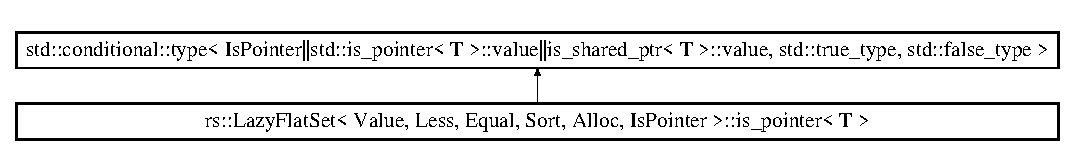
\includegraphics[height=1.644640cm]{structrs_1_1_lazy_flat_set_1_1is__pointer}
\end{center}
\end{figure}


The documentation for this struct was generated from the following file\+:\begin{DoxyCompactItemize}
\item 
Utilities/lazyflatset.\+hpp\end{DoxyCompactItemize}

\hypertarget{structrs_1_1_lazy_flat_set_1_1is__shared__ptr}{\section{rs\+:\+:Lazy\+Flat\+Set$<$ Value, Less, Equal, Sort, Alloc, Is\+Pointer $>$\+:\+:is\+\_\+shared\+\_\+ptr$<$ T $>$ Struct Template Reference}
\label{structrs_1_1_lazy_flat_set_1_1is__shared__ptr}\index{rs\+::\+Lazy\+Flat\+Set$<$ Value, Less, Equal, Sort, Alloc, Is\+Pointer $>$\+::is\+\_\+shared\+\_\+ptr$<$ T $>$@{rs\+::\+Lazy\+Flat\+Set$<$ Value, Less, Equal, Sort, Alloc, Is\+Pointer $>$\+::is\+\_\+shared\+\_\+ptr$<$ T $>$}}
}
Inheritance diagram for rs\+:\+:Lazy\+Flat\+Set$<$ Value, Less, Equal, Sort, Alloc, Is\+Pointer $>$\+:\+:is\+\_\+shared\+\_\+ptr$<$ T $>$\+:\begin{figure}[H]
\begin{center}
\leavevmode
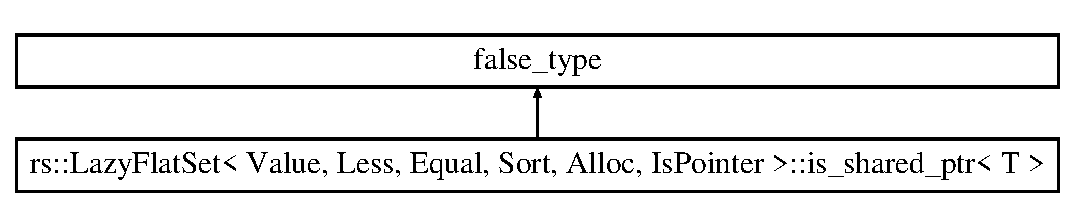
\includegraphics[height=2.000000cm]{structrs_1_1_lazy_flat_set_1_1is__shared__ptr}
\end{center}
\end{figure}


The documentation for this struct was generated from the following file\+:\begin{DoxyCompactItemize}
\item 
Utilities/lazyflatset.\+hpp\end{DoxyCompactItemize}

\hypertarget{structrs_1_1_lazy_flat_set_1_1is__shared__ptr_3_01std_1_1shared__ptr_3_01_t_01_4_01_4}{\section{rs\+:\+:Lazy\+Flat\+Set$<$ Value, Less, Equal, Sort, Alloc, Is\+Pointer $>$\+:\+:is\+\_\+shared\+\_\+ptr$<$ std\+:\+:shared\+\_\+ptr$<$ T $>$ $>$ Struct Template Reference}
\label{structrs_1_1_lazy_flat_set_1_1is__shared__ptr_3_01std_1_1shared__ptr_3_01_t_01_4_01_4}\index{rs\+::\+Lazy\+Flat\+Set$<$ Value, Less, Equal, Sort, Alloc, Is\+Pointer $>$\+::is\+\_\+shared\+\_\+ptr$<$ std\+::shared\+\_\+ptr$<$ T $>$ $>$@{rs\+::\+Lazy\+Flat\+Set$<$ Value, Less, Equal, Sort, Alloc, Is\+Pointer $>$\+::is\+\_\+shared\+\_\+ptr$<$ std\+::shared\+\_\+ptr$<$ T $>$ $>$}}
}
Inheritance diagram for rs\+:\+:Lazy\+Flat\+Set$<$ Value, Less, Equal, Sort, Alloc, Is\+Pointer $>$\+:\+:is\+\_\+shared\+\_\+ptr$<$ std\+:\+:shared\+\_\+ptr$<$ T $>$ $>$\+:\begin{figure}[H]
\begin{center}
\leavevmode
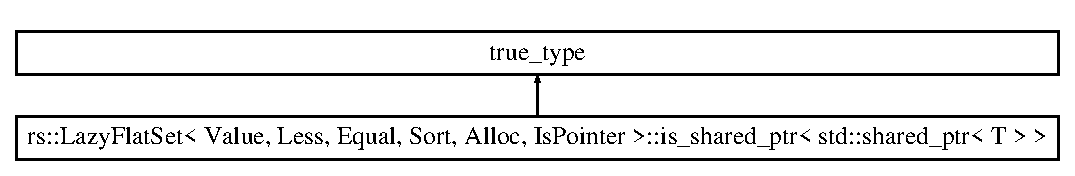
\includegraphics[height=1.917808cm]{structrs_1_1_lazy_flat_set_1_1is__shared__ptr_3_01std_1_1shared__ptr_3_01_t_01_4_01_4}
\end{center}
\end{figure}


The documentation for this struct was generated from the following file\+:\begin{DoxyCompactItemize}
\item 
Utilities/lazyflatset.\+hpp\end{DoxyCompactItemize}

\hypertarget{classemlib_1_1_hash_map_1_1iterator}{\section{emlib\+:\+:Hash\+Map$<$ Key\+T, Value\+T, Hash\+T, Comp\+T $>$\+:\+:iterator Class Reference}
\label{classemlib_1_1_hash_map_1_1iterator}\index{emlib\+::\+Hash\+Map$<$ Key\+T, Value\+T, Hash\+T, Comp\+T $>$\+::iterator@{emlib\+::\+Hash\+Map$<$ Key\+T, Value\+T, Hash\+T, Comp\+T $>$\+::iterator}}
}
\subsection*{Public Types}
\begin{DoxyCompactItemize}
\item 
\hypertarget{classemlib_1_1_hash_map_1_1iterator_afa7c05ed56ee72d7b5d94997df10b8a6}{using {\bfseries iterator\+\_\+category} = std\+::forward\+\_\+iterator\+\_\+tag}\label{classemlib_1_1_hash_map_1_1iterator_afa7c05ed56ee72d7b5d94997df10b8a6}

\item 
\hypertarget{classemlib_1_1_hash_map_1_1iterator_a91e5ebf00ae7d62f6764c24a01023a1d}{using {\bfseries difference\+\_\+type} = size\+\_\+t}\label{classemlib_1_1_hash_map_1_1iterator_a91e5ebf00ae7d62f6764c24a01023a1d}

\item 
\hypertarget{classemlib_1_1_hash_map_1_1iterator_a0210f1729113f998066815e6148b5b76}{using {\bfseries distance\+\_\+type} = size\+\_\+t}\label{classemlib_1_1_hash_map_1_1iterator_a0210f1729113f998066815e6148b5b76}

\item 
\hypertarget{classemlib_1_1_hash_map_1_1iterator_ac812c6ea0339570a6f6f6e300d42063b}{using {\bfseries value\+\_\+type} = std\+::pair$<$ Key\+T, Value\+T $>$}\label{classemlib_1_1_hash_map_1_1iterator_ac812c6ea0339570a6f6f6e300d42063b}

\item 
\hypertarget{classemlib_1_1_hash_map_1_1iterator_a1c9980515ea3f12e8b6bca06c3f14d0d}{using {\bfseries pointer} = value\+\_\+type $\ast$}\label{classemlib_1_1_hash_map_1_1iterator_a1c9980515ea3f12e8b6bca06c3f14d0d}

\item 
\hypertarget{classemlib_1_1_hash_map_1_1iterator_abf4d4a39e97a8923b29f8261fe1a4c81}{using {\bfseries reference} = value\+\_\+type \&}\label{classemlib_1_1_hash_map_1_1iterator_abf4d4a39e97a8923b29f8261fe1a4c81}

\end{DoxyCompactItemize}
\subsection*{Public Member Functions}
\begin{DoxyCompactItemize}
\item 
\hypertarget{classemlib_1_1_hash_map_1_1iterator_adb65aeacd8b684e1cb621475f67c4ce8}{{\bfseries iterator} (\hyperlink{classemlib_1_1_hash_map}{My\+Type} $\ast$hash\+\_\+map, size\+\_\+t bucket)}\label{classemlib_1_1_hash_map_1_1iterator_adb65aeacd8b684e1cb621475f67c4ce8}

\item 
\hypertarget{classemlib_1_1_hash_map_1_1iterator_a7be8de78e4adeee72d45218e7e91ea58}{\hyperlink{classemlib_1_1_hash_map_1_1iterator}{iterator} \& {\bfseries operator++} ()}\label{classemlib_1_1_hash_map_1_1iterator_a7be8de78e4adeee72d45218e7e91ea58}

\item 
\hypertarget{classemlib_1_1_hash_map_1_1iterator_a19708502ad7631df0189b2905649a7ed}{\hyperlink{classemlib_1_1_hash_map_1_1iterator}{iterator} {\bfseries operator++} (int)}\label{classemlib_1_1_hash_map_1_1iterator_a19708502ad7631df0189b2905649a7ed}

\item 
\hypertarget{classemlib_1_1_hash_map_1_1iterator_aa7e8ec41fb953ee372fcd9733b44966f}{reference {\bfseries operator$\ast$} () const }\label{classemlib_1_1_hash_map_1_1iterator_aa7e8ec41fb953ee372fcd9733b44966f}

\item 
\hypertarget{classemlib_1_1_hash_map_1_1iterator_a496b74ac273b83dd66939709b8e2c37e}{pointer {\bfseries operator-\/$>$} () const }\label{classemlib_1_1_hash_map_1_1iterator_a496b74ac273b83dd66939709b8e2c37e}

\item 
\hypertarget{classemlib_1_1_hash_map_1_1iterator_ac842985c03a07027eb3cf8c87b277050}{bool {\bfseries operator==} (const \hyperlink{classemlib_1_1_hash_map_1_1iterator}{iterator} \&rhs)}\label{classemlib_1_1_hash_map_1_1iterator_ac842985c03a07027eb3cf8c87b277050}

\item 
\hypertarget{classemlib_1_1_hash_map_1_1iterator_a2382b9e7b174d08c8d7a5a99e562f09b}{bool {\bfseries operator!=} (const \hyperlink{classemlib_1_1_hash_map_1_1iterator}{iterator} \&rhs)}\label{classemlib_1_1_hash_map_1_1iterator_a2382b9e7b174d08c8d7a5a99e562f09b}

\end{DoxyCompactItemize}
\subsection*{Public Attributes}
\begin{DoxyCompactItemize}
\item 
\hypertarget{classemlib_1_1_hash_map_1_1iterator_ac7fc941bccf75991d28dd9add54f1dfe}{\hyperlink{classemlib_1_1_hash_map}{My\+Type} $\ast$ {\bfseries \+\_\+map}}\label{classemlib_1_1_hash_map_1_1iterator_ac7fc941bccf75991d28dd9add54f1dfe}

\item 
\hypertarget{classemlib_1_1_hash_map_1_1iterator_ab296237c255b76c699594673d42d1fcd}{size\+\_\+t {\bfseries \+\_\+bucket}}\label{classemlib_1_1_hash_map_1_1iterator_ab296237c255b76c699594673d42d1fcd}

\end{DoxyCompactItemize}


The documentation for this class was generated from the following file\+:\begin{DoxyCompactItemize}
\item 
third\+\_\+party/Hash\+Containers.\+hpp\end{DoxyCompactItemize}

\hypertarget{classemlib_1_1_hash_set_1_1iterator}{\section{emlib\+:\+:Hash\+Set$<$ Key\+T, Hash\+T, Comp\+T $>$\+:\+:iterator Class Reference}
\label{classemlib_1_1_hash_set_1_1iterator}\index{emlib\+::\+Hash\+Set$<$ Key\+T, Hash\+T, Comp\+T $>$\+::iterator@{emlib\+::\+Hash\+Set$<$ Key\+T, Hash\+T, Comp\+T $>$\+::iterator}}
}
\subsection*{Public Types}
\begin{DoxyCompactItemize}
\item 
\hypertarget{classemlib_1_1_hash_set_1_1iterator_a69af29529d085f44809d77e67d036fb7}{using {\bfseries iterator\+\_\+category} = std\+::forward\+\_\+iterator\+\_\+tag}\label{classemlib_1_1_hash_set_1_1iterator_a69af29529d085f44809d77e67d036fb7}

\item 
\hypertarget{classemlib_1_1_hash_set_1_1iterator_a7d59c912800ffd292ff8cf1ae78af99a}{using {\bfseries difference\+\_\+type} = size\+\_\+t}\label{classemlib_1_1_hash_set_1_1iterator_a7d59c912800ffd292ff8cf1ae78af99a}

\item 
\hypertarget{classemlib_1_1_hash_set_1_1iterator_a7f6ede0a87277d38492f729434409eb9}{using {\bfseries distance\+\_\+type} = size\+\_\+t}\label{classemlib_1_1_hash_set_1_1iterator_a7f6ede0a87277d38492f729434409eb9}

\item 
\hypertarget{classemlib_1_1_hash_set_1_1iterator_ac200afa0b3308030d90214cf27ea1611}{using {\bfseries value\+\_\+type} = Key\+T}\label{classemlib_1_1_hash_set_1_1iterator_ac200afa0b3308030d90214cf27ea1611}

\item 
\hypertarget{classemlib_1_1_hash_set_1_1iterator_af31b6d66e9ce1bcdaef1eff25d48b351}{using {\bfseries pointer} = value\+\_\+type $\ast$}\label{classemlib_1_1_hash_set_1_1iterator_af31b6d66e9ce1bcdaef1eff25d48b351}

\item 
\hypertarget{classemlib_1_1_hash_set_1_1iterator_a24abd72780f2ebfadd2bfd5ac82fed3e}{using {\bfseries reference} = value\+\_\+type \&}\label{classemlib_1_1_hash_set_1_1iterator_a24abd72780f2ebfadd2bfd5ac82fed3e}

\end{DoxyCompactItemize}
\subsection*{Public Member Functions}
\begin{DoxyCompactItemize}
\item 
\hypertarget{classemlib_1_1_hash_set_1_1iterator_af62e79eae2bc973529a83cc8ec9ec9a0}{{\bfseries iterator} (\hyperlink{classemlib_1_1_hash_set}{My\+Type} $\ast$hash\+\_\+set, size\+\_\+t bucket)}\label{classemlib_1_1_hash_set_1_1iterator_af62e79eae2bc973529a83cc8ec9ec9a0}

\item 
\hypertarget{classemlib_1_1_hash_set_1_1iterator_aa808a7bf4c269ff744f644f499fabc3d}{\hyperlink{classemlib_1_1_hash_set_1_1iterator}{iterator} \& {\bfseries operator++} ()}\label{classemlib_1_1_hash_set_1_1iterator_aa808a7bf4c269ff744f644f499fabc3d}

\item 
\hypertarget{classemlib_1_1_hash_set_1_1iterator_ac4dd53857daa7c18fd1b9cf8b67cb515}{\hyperlink{classemlib_1_1_hash_set_1_1iterator}{iterator} {\bfseries operator++} (int)}\label{classemlib_1_1_hash_set_1_1iterator_ac4dd53857daa7c18fd1b9cf8b67cb515}

\item 
\hypertarget{classemlib_1_1_hash_set_1_1iterator_a2bed19dc8f82b2453de665243b0aa0b2}{reference {\bfseries operator$\ast$} () const }\label{classemlib_1_1_hash_set_1_1iterator_a2bed19dc8f82b2453de665243b0aa0b2}

\item 
\hypertarget{classemlib_1_1_hash_set_1_1iterator_a0fd7cd3829b64a895c24838a8a9355a0}{pointer {\bfseries operator-\/$>$} () const }\label{classemlib_1_1_hash_set_1_1iterator_a0fd7cd3829b64a895c24838a8a9355a0}

\item 
\hypertarget{classemlib_1_1_hash_set_1_1iterator_a319dd1ea6f9255c6342e57055cb27cef}{bool {\bfseries operator==} (const \hyperlink{classemlib_1_1_hash_set_1_1iterator}{iterator} \&rhs)}\label{classemlib_1_1_hash_set_1_1iterator_a319dd1ea6f9255c6342e57055cb27cef}

\item 
\hypertarget{classemlib_1_1_hash_set_1_1iterator_a950ce3bc68a8877bade24aaa3c8d4c06}{bool {\bfseries operator!=} (const \hyperlink{classemlib_1_1_hash_set_1_1iterator}{iterator} \&rhs)}\label{classemlib_1_1_hash_set_1_1iterator_a950ce3bc68a8877bade24aaa3c8d4c06}

\end{DoxyCompactItemize}
\subsection*{Public Attributes}
\begin{DoxyCompactItemize}
\item 
\hypertarget{classemlib_1_1_hash_set_1_1iterator_af5e8cf31b2ce7567932aa1f8c44f4219}{\hyperlink{classemlib_1_1_hash_set}{My\+Type} $\ast$ {\bfseries \+\_\+set}}\label{classemlib_1_1_hash_set_1_1iterator_af5e8cf31b2ce7567932aa1f8c44f4219}

\item 
\hypertarget{classemlib_1_1_hash_set_1_1iterator_aff615f5180b0a2e76ff027256c25af73}{size\+\_\+t {\bfseries \+\_\+bucket}}\label{classemlib_1_1_hash_set_1_1iterator_aff615f5180b0a2e76ff027256c25af73}

\end{DoxyCompactItemize}


The documentation for this class was generated from the following file\+:\begin{DoxyCompactItemize}
\item 
third\+\_\+party/Hash\+Containers.\+hpp\end{DoxyCompactItemize}

\hypertarget{classrs_1_1_lazy_flat_set}{\section{rs\+:\+:Lazy\+Flat\+Set$<$ Value, Less, Equal, Sort, Alloc, Is\+Pointer $>$ Class Template Reference}
\label{classrs_1_1_lazy_flat_set}\index{rs\+::\+Lazy\+Flat\+Set$<$ Value, Less, Equal, Sort, Alloc, Is\+Pointer $>$@{rs\+::\+Lazy\+Flat\+Set$<$ Value, Less, Equal, Sort, Alloc, Is\+Pointer $>$}}
}
\subsection*{Classes}
\begin{DoxyCompactItemize}
\item 
struct \hyperlink{structrs_1_1_lazy_flat_set_1_1is__pointer}{is\+\_\+pointer}
\item 
struct \hyperlink{structrs_1_1_lazy_flat_set_1_1is__shared__ptr}{is\+\_\+shared\+\_\+ptr}
\item 
struct \hyperlink{structrs_1_1_lazy_flat_set_1_1is__shared__ptr_3_01std_1_1shared__ptr_3_01_t_01_4_01_4}{is\+\_\+shared\+\_\+ptr$<$ std\+::shared\+\_\+ptr$<$ T $>$ $>$}
\end{DoxyCompactItemize}
\subsection*{Public Types}
\begin{DoxyCompactItemize}
\item 
\hypertarget{classrs_1_1_lazy_flat_set_adf2eab7a354a5d355d59ca7f15133d1d}{using {\bfseries base\+\_\+collection} = typename std\+::vector$<$ Value, Alloc $>$}\label{classrs_1_1_lazy_flat_set_adf2eab7a354a5d355d59ca7f15133d1d}

\item 
\hypertarget{classrs_1_1_lazy_flat_set_a6e0778124a9f2727c188c43c129cf34b}{using {\bfseries size\+\_\+type} = typename base\+\_\+collection\+::size\+\_\+type}\label{classrs_1_1_lazy_flat_set_a6e0778124a9f2727c188c43c129cf34b}

\item 
\hypertarget{classrs_1_1_lazy_flat_set_a49d91b95a28692e53ab6b0a487862065}{using {\bfseries iterator} = typename base\+\_\+collection\+::iterator}\label{classrs_1_1_lazy_flat_set_a49d91b95a28692e53ab6b0a487862065}

\item 
\hypertarget{classrs_1_1_lazy_flat_set_a3060161b3a52f713d086620993093a59}{using {\bfseries const\+\_\+iterator} = typename base\+\_\+collection\+::const\+\_\+iterator}\label{classrs_1_1_lazy_flat_set_a3060161b3a52f713d086620993093a59}

\item 
\hypertarget{classrs_1_1_lazy_flat_set_ab7de742924e7b252dab47f93990785fb}{using {\bfseries value\+\_\+type} = Value}\label{classrs_1_1_lazy_flat_set_ab7de742924e7b252dab47f93990785fb}

\item 
\hypertarget{classrs_1_1_lazy_flat_set_a49156f05e1342af92e1499952606c1f1}{using {\bfseries value\+\_\+type\+\_\+ptr} = typename std\+::conditional$<$ \hyperlink{structrs_1_1_lazy_flat_set_1_1is__pointer}{is\+\_\+pointer}$<$ value\+\_\+type $>$\+::value, value\+\_\+type, value\+\_\+type $\ast$ $>$\+::type}\label{classrs_1_1_lazy_flat_set_a49156f05e1342af92e1499952606c1f1}

\item 
\hypertarget{classrs_1_1_lazy_flat_set_aa53ec129bdf69cce6fd44e08bef795d1}{using {\bfseries reference} = typename std\+::conditional$<$ std\+::is\+\_\+fundamental$<$ value\+\_\+type $>$\+::value$\vert$$\vert$std\+::is\+\_\+pointer$<$ value\+\_\+type $>$\+::value, value\+\_\+type, value\+\_\+type \& $>$\+::type}\label{classrs_1_1_lazy_flat_set_aa53ec129bdf69cce6fd44e08bef795d1}

\item 
\hypertarget{classrs_1_1_lazy_flat_set_a1eee0250aeecaaa0bc0c52ed44c44103}{using {\bfseries const\+\_\+reference} = typename std\+::conditional$<$ std\+::is\+\_\+fundamental$<$ value\+\_\+type $>$\+::value$\vert$$\vert$std\+::is\+\_\+pointer$<$ value\+\_\+type $>$\+::value, value\+\_\+type, const value\+\_\+type \& $>$\+::type}\label{classrs_1_1_lazy_flat_set_a1eee0250aeecaaa0bc0c52ed44c44103}

\item 
\hypertarget{classrs_1_1_lazy_flat_set_ad62702a8dd24dd6994f6de93a95ac06b}{using {\bfseries less\+\_\+type} = Less}\label{classrs_1_1_lazy_flat_set_ad62702a8dd24dd6994f6de93a95ac06b}

\item 
\hypertarget{classrs_1_1_lazy_flat_set_a4ceed88565e4ec459cabaa95d08b7543}{using {\bfseries equal\+\_\+type} = Equal}\label{classrs_1_1_lazy_flat_set_a4ceed88565e4ec459cabaa95d08b7543}

\item 
\hypertarget{classrs_1_1_lazy_flat_set_ad8b2f85dadbdab6708ea958a92efea81}{using {\bfseries sort\+\_\+type} = Sort}\label{classrs_1_1_lazy_flat_set_ad8b2f85dadbdab6708ea958a92efea81}

\item 
\hypertarget{classrs_1_1_lazy_flat_set_a3a7384c560080249b45a5f244859e7dd}{using {\bfseries alloc\+\_\+type} = Alloc}\label{classrs_1_1_lazy_flat_set_a3a7384c560080249b45a5f244859e7dd}

\item 
\hypertarget{classrs_1_1_lazy_flat_set_a8b0320d955fffb1457c512191b5f0b0b}{using {\bfseries compare\+\_\+type} = typename std\+::function$<$ int(const\+\_\+reference)$>$}\label{classrs_1_1_lazy_flat_set_a8b0320d955fffb1457c512191b5f0b0b}

\item 
\hypertarget{classrs_1_1_lazy_flat_set_add721f9ad9f6a52a08b31cf1f3b773fd}{using {\bfseries erase\+\_\+type} = typename std\+::function$<$ void(reference)$>$}\label{classrs_1_1_lazy_flat_set_add721f9ad9f6a52a08b31cf1f3b773fd}

\end{DoxyCompactItemize}
\subsection*{Public Member Functions}
\begin{DoxyCompactItemize}
\item 
\hypertarget{classrs_1_1_lazy_flat_set_a9ea0bbd4e1d94533137a9b56ccac7d4c}{{\bfseries Lazy\+Flat\+Set} (unsigned max\+Unsorted\+Entries=16, unsigned max\+Nursery\+Entries=1024)}\label{classrs_1_1_lazy_flat_set_a9ea0bbd4e1d94533137a9b56ccac7d4c}

\item 
\hypertarget{classrs_1_1_lazy_flat_set_a4d054f28cda0cc8f121f744ef51ff522}{void {\bfseries insert} (const value\+\_\+type \&k)}\label{classrs_1_1_lazy_flat_set_a4d054f28cda0cc8f121f744ef51ff522}

\item 
\hypertarget{classrs_1_1_lazy_flat_set_af0a6a89258598652bd3427dd30f305d7}{{\footnotesize template$<$typename... Args$>$ }\\void {\bfseries emplace} (Args \&\&...args)}\label{classrs_1_1_lazy_flat_set_af0a6a89258598652bd3427dd30f305d7}

\item 
\hypertarget{classrs_1_1_lazy_flat_set_a48f842cd25a139242cd765727c710d74}{bool {\bfseries empty} () const }\label{classrs_1_1_lazy_flat_set_a48f842cd25a139242cd765727c710d74}

\item 
\hypertarget{classrs_1_1_lazy_flat_set_aff614815c0687575e57c2ceb7d8ea404}{void {\bfseries clear} ()}\label{classrs_1_1_lazy_flat_set_aff614815c0687575e57c2ceb7d8ea404}

\item 
\hypertarget{classrs_1_1_lazy_flat_set_a41a13387ae1d139cc272a72ab5cf9a6d}{void {\bfseries clear\+\_\+fn} (erase\+\_\+type erase)}\label{classrs_1_1_lazy_flat_set_a41a13387ae1d139cc272a72ab5cf9a6d}

\item 
\hypertarget{classrs_1_1_lazy_flat_set_a5520dcf84139948db4a0ac404aa46b5d}{void {\bfseries reserve} (size\+\_\+type n)}\label{classrs_1_1_lazy_flat_set_a5520dcf84139948db4a0ac404aa46b5d}

\item 
\hypertarget{classrs_1_1_lazy_flat_set_a87442717551e748854bc2579630fc929}{size\+\_\+type {\bfseries size} () const }\label{classrs_1_1_lazy_flat_set_a87442717551e748854bc2579630fc929}

\item 
\hypertarget{classrs_1_1_lazy_flat_set_abd6bf510bda52919c5cbaaa3f100315b}{void {\bfseries shrink\+\_\+to\+\_\+fit} ()}\label{classrs_1_1_lazy_flat_set_abd6bf510bda52919c5cbaaa3f100315b}

\item 
\hypertarget{classrs_1_1_lazy_flat_set_a453db2cb99f2a2460587357d6172f53d}{size\+\_\+type {\bfseries count} (const value\+\_\+type \&k) const }\label{classrs_1_1_lazy_flat_set_a453db2cb99f2a2460587357d6172f53d}

\item 
\hypertarget{classrs_1_1_lazy_flat_set_a858b3de5ef175c352b0de597605a4651}{size\+\_\+type {\bfseries count\+\_\+fn} (compare\+\_\+type compare) const }\label{classrs_1_1_lazy_flat_set_a858b3de5ef175c352b0de597605a4651}

\item 
\hypertarget{classrs_1_1_lazy_flat_set_aaaac3c19a0d0ae902fa46528ca0e1951}{bool {\bfseries find} (const value\+\_\+type \&k, value\+\_\+type \&v) const }\label{classrs_1_1_lazy_flat_set_aaaac3c19a0d0ae902fa46528ca0e1951}

\item 
\hypertarget{classrs_1_1_lazy_flat_set_a2f67bfa2c404bb3ce9723e5760b9174e}{value\+\_\+type\+\_\+ptr {\bfseries find\+\_\+fn} (compare\+\_\+type compare) const }\label{classrs_1_1_lazy_flat_set_a2f67bfa2c404bb3ce9723e5760b9174e}

\item 
\hypertarget{classrs_1_1_lazy_flat_set_a89b957974d573d58f76a893a793f6a2f}{const\+\_\+reference {\bfseries operator\mbox{[}$\,$\mbox{]}} (size\+\_\+type n) const }\label{classrs_1_1_lazy_flat_set_a89b957974d573d58f76a893a793f6a2f}

\item 
\hypertarget{classrs_1_1_lazy_flat_set_a7682d5040699a6e5780a50803b692f40}{const\+\_\+iterator {\bfseries cbegin} () const }\label{classrs_1_1_lazy_flat_set_a7682d5040699a6e5780a50803b692f40}

\item 
\hypertarget{classrs_1_1_lazy_flat_set_a7a405e2401d17db44397bced6584fabb}{const\+\_\+iterator {\bfseries cend} () const }\label{classrs_1_1_lazy_flat_set_a7a405e2401d17db44397bced6584fabb}

\item 
\hypertarget{classrs_1_1_lazy_flat_set_ab9eed6a6e5f47a3f06f1b5ad21628043}{const value\+\_\+type $\ast$ {\bfseries data} () const }\label{classrs_1_1_lazy_flat_set_ab9eed6a6e5f47a3f06f1b5ad21628043}

\item 
\hypertarget{classrs_1_1_lazy_flat_set_a7cb8ec3c50be5045260bcb9dc631f146}{size\+\_\+type {\bfseries erase} (const value\+\_\+type \&k)}\label{classrs_1_1_lazy_flat_set_a7cb8ec3c50be5045260bcb9dc631f146}

\item 
\hypertarget{classrs_1_1_lazy_flat_set_a9a2b9f5c6ef29071724c5f4e9c060a61}{size\+\_\+type {\bfseries erase\+\_\+fn} (compare\+\_\+type compare, erase\+\_\+type erase=nullptr)}\label{classrs_1_1_lazy_flat_set_a9a2b9f5c6ef29071724c5f4e9c060a61}

\item 
\hypertarget{classrs_1_1_lazy_flat_set_aad6954260bbb8d00e3f4214edbac8d52}{void {\bfseries copy} (std\+::vector$<$ Value $>$ \&coll, bool sort=true) const }\label{classrs_1_1_lazy_flat_set_aad6954260bbb8d00e3f4214edbac8d52}

\end{DoxyCompactItemize}


The documentation for this class was generated from the following file\+:\begin{DoxyCompactItemize}
\item 
Utilities/lazyflatset.\+hpp\end{DoxyCompactItemize}

\hypertarget{structrs_1_1_lazy_flat_set_quick_sort}{\section{rs\+:\+:Lazy\+Flat\+Set\+Quick\+Sort$<$ Value, Less $>$ Struct Template Reference}
\label{structrs_1_1_lazy_flat_set_quick_sort}\index{rs\+::\+Lazy\+Flat\+Set\+Quick\+Sort$<$ Value, Less $>$@{rs\+::\+Lazy\+Flat\+Set\+Quick\+Sort$<$ Value, Less $>$}}
}
\subsection*{Public Member Functions}
\begin{DoxyCompactItemize}
\item 
\hypertarget{structrs_1_1_lazy_flat_set_quick_sort_a6589a914256756b7cd152cdf2c0f2cef}{void {\bfseries operator()} (typename \hyperlink{classrs_1_1_lazy_flat_set}{Lazy\+Flat\+Set}$<$ Value $>$\+::iterator first, typename \hyperlink{classrs_1_1_lazy_flat_set}{Lazy\+Flat\+Set}$<$ Value $>$\+::iterator last)}\label{structrs_1_1_lazy_flat_set_quick_sort_a6589a914256756b7cd152cdf2c0f2cef}

\end{DoxyCompactItemize}


The documentation for this struct was generated from the following file\+:\begin{DoxyCompactItemize}
\item 
Utilities/lazyflatset.\+hpp\end{DoxyCompactItemize}

\hypertarget{classlevelorder__vector}{\section{levelorder\+\_\+vector$<$ T $>$ Class Template Reference}
\label{classlevelorder__vector}\index{levelorder\+\_\+vector$<$ T $>$@{levelorder\+\_\+vector$<$ T $>$}}
}
\subsection*{Public Types}
\begin{DoxyCompactItemize}
\item 
\hypertarget{classlevelorder__vector_a8b4bb6dee5a810a0d328546b68feba12}{typedef vector\+::value\+\_\+type {\bfseries value\+\_\+type}}\label{classlevelorder__vector_a8b4bb6dee5a810a0d328546b68feba12}

\item 
\hypertarget{classlevelorder__vector_a0786df56083511c2feba7a29c418ddc5}{typedef vector\+::reference {\bfseries reference}}\label{classlevelorder__vector_a0786df56083511c2feba7a29c418ddc5}

\item 
\hypertarget{classlevelorder__vector_a87776a7480ed0fa7ff2fcd9c258dc8ad}{typedef vector\+::const\+\_\+reference {\bfseries const\+\_\+reference}}\label{classlevelorder__vector_a87776a7480ed0fa7ff2fcd9c258dc8ad}

\item 
\hypertarget{classlevelorder__vector_a1421e59d3f55cc9e7da10d5399182912}{typedef vector\+::const\+\_\+iterator {\bfseries iterator}}\label{classlevelorder__vector_a1421e59d3f55cc9e7da10d5399182912}

\item 
\hypertarget{classlevelorder__vector_a1f2520e9561b990c74ebccb2ee5fa576}{typedef vector\+::const\+\_\+iterator {\bfseries const\+\_\+iterator}}\label{classlevelorder__vector_a1f2520e9561b990c74ebccb2ee5fa576}

\item 
\hypertarget{classlevelorder__vector_a7362366fdf73647346d8699270ae0a46}{typedef vector\+::difference\+\_\+type {\bfseries difference\+\_\+type}}\label{classlevelorder__vector_a7362366fdf73647346d8699270ae0a46}

\item 
\hypertarget{classlevelorder__vector_a3ed08ee68fdd65c7db5aedf7a9641065}{typedef vector\+::size\+\_\+type {\bfseries size\+\_\+type}}\label{classlevelorder__vector_a3ed08ee68fdd65c7db5aedf7a9641065}

\end{DoxyCompactItemize}
\subsection*{Public Member Functions}
\begin{DoxyCompactItemize}
\item 
\hypertarget{classlevelorder__vector_a6960833289a781ec6d56216c38d3b13b}{{\bfseries levelorder\+\_\+vector} (const \hyperlink{classlevelorder__vector}{levelorder\+\_\+vector} \&x)}\label{classlevelorder__vector_a6960833289a781ec6d56216c38d3b13b}

\item 
\hypertarget{classlevelorder__vector_ad7d17bbade58e06cef0b1c52b456bd1c}{\hyperlink{classlevelorder__vector}{levelorder\+\_\+vector} \& {\bfseries operator=} (const \hyperlink{classlevelorder__vector}{levelorder\+\_\+vector} \&x)}\label{classlevelorder__vector_ad7d17bbade58e06cef0b1c52b456bd1c}

\item 
\hypertarget{classlevelorder__vector_afae5b9bc9acafd65738acbb0be43e09e}{{\footnotesize template$<$typename Input\+Iterator $>$ }\\{\bfseries levelorder\+\_\+vector} (Input\+Iterator first, Input\+Iterator last)}\label{classlevelorder__vector_afae5b9bc9acafd65738acbb0be43e09e}

\item 
\hypertarget{classlevelorder__vector_a99ad7144ea654480177bd3b4c91fd602}{const\+\_\+iterator {\bfseries begin} () const }\label{classlevelorder__vector_a99ad7144ea654480177bd3b4c91fd602}

\item 
\hypertarget{classlevelorder__vector_a469ea8a51923cd674f42703b8a10b336}{const\+\_\+iterator {\bfseries end} () const }\label{classlevelorder__vector_a469ea8a51923cd674f42703b8a10b336}

\item 
\hypertarget{classlevelorder__vector_a6f080dd85f82fe429da7957518d81173}{const\+\_\+iterator {\bfseries cbegin} () const }\label{classlevelorder__vector_a6f080dd85f82fe429da7957518d81173}

\item 
\hypertarget{classlevelorder__vector_a42f7fee4cbad60eb58ac2b6ed8fad559}{const\+\_\+iterator {\bfseries cend} () const }\label{classlevelorder__vector_a42f7fee4cbad60eb58ac2b6ed8fad559}

\item 
\hypertarget{classlevelorder__vector_a3d8690970562fde45a9b406a4bfe9908}{void {\bfseries swap} (\hyperlink{classlevelorder__vector}{levelorder\+\_\+vector} \&x)}\label{classlevelorder__vector_a3d8690970562fde45a9b406a4bfe9908}

\item 
\hypertarget{classlevelorder__vector_aa5aec8c6252e268b3f1b4fe2457b553c}{size\+\_\+type {\bfseries size} () const }\label{classlevelorder__vector_aa5aec8c6252e268b3f1b4fe2457b553c}

\item 
\hypertarget{classlevelorder__vector_a6f584af619e77dd5bdebf311f2d5b189}{size\+\_\+type {\bfseries max\+\_\+size} () const }\label{classlevelorder__vector_a6f584af619e77dd5bdebf311f2d5b189}

\item 
\hypertarget{classlevelorder__vector_a67cf39f7dfa8e8c139b320303ed93f3e}{bool {\bfseries empty} () const }\label{classlevelorder__vector_a67cf39f7dfa8e8c139b320303ed93f3e}

\item 
\hypertarget{classlevelorder__vector_a8c54c5e980c17dc0de64a046427ce275}{const\+\_\+iterator {\bfseries lower\+\_\+bound} (const T \&x) const }\label{classlevelorder__vector_a8c54c5e980c17dc0de64a046427ce275}

\item 
\hypertarget{classlevelorder__vector_a4cfb32f7ca9980d20a97b3ab910c257f}{void {\bfseries build} ()}\label{classlevelorder__vector_a4cfb32f7ca9980d20a97b3ab910c257f}

\item 
\hypertarget{classlevelorder__vector_a4bb13b1b043ed0a140fb4d356eb5aa9e}{void {\bfseries push} (const T \&t)}\label{classlevelorder__vector_a4bb13b1b043ed0a140fb4d356eb5aa9e}

\item 
\hypertarget{classlevelorder__vector_a6599405b77b76d01290b10df5f1f8c88}{void {\bfseries clear} ()}\label{classlevelorder__vector_a6599405b77b76d01290b10df5f1f8c88}

\item 
\hypertarget{classlevelorder__vector_aab03ef5b075e0ca1080d2db385234013}{void {\bfseries clear\+\_\+no\+\_\+resize} ()}\label{classlevelorder__vector_aab03ef5b075e0ca1080d2db385234013}

\end{DoxyCompactItemize}
\subsection*{Friends}
\begin{DoxyCompactItemize}
\item 
\hypertarget{classlevelorder__vector_adc84f538ec738d4d9526a404b29985be}{bool {\bfseries operator==} (const \hyperlink{classlevelorder__vector}{levelorder\+\_\+vector} \&x, const \hyperlink{classlevelorder__vector}{levelorder\+\_\+vector} \&y)}\label{classlevelorder__vector_adc84f538ec738d4d9526a404b29985be}

\item 
\hypertarget{classlevelorder__vector_ae62086a3d9f47df4b3a794f705be5124}{bool {\bfseries operator!=} (const \hyperlink{classlevelorder__vector}{levelorder\+\_\+vector} \&x, const \hyperlink{classlevelorder__vector}{levelorder\+\_\+vector} \&y)}\label{classlevelorder__vector_ae62086a3d9f47df4b3a794f705be5124}

\item 
\hypertarget{classlevelorder__vector_a8a40c8b3cb31bf40c2142f514f4ce125}{void {\bfseries swap} (\hyperlink{classlevelorder__vector}{levelorder\+\_\+vector} \&x, \hyperlink{classlevelorder__vector}{levelorder\+\_\+vector} \&y)}\label{classlevelorder__vector_a8a40c8b3cb31bf40c2142f514f4ce125}

\end{DoxyCompactItemize}


The documentation for this class was generated from the following file\+:\begin{DoxyCompactItemize}
\item 
Utilities/flat\+\_\+set.\+hpp\end{DoxyCompactItemize}

\hypertarget{classatl_1_1_line_plot}{\section{atl\+:\+:Line\+Plot$<$ T $>$ Class Template Reference}
\label{classatl_1_1_line_plot}\index{atl\+::\+Line\+Plot$<$ T $>$@{atl\+::\+Line\+Plot$<$ T $>$}}
}


The documentation for this class was generated from the following file\+:\begin{DoxyCompactItemize}
\item 
Utilities/Plots.\+hpp\end{DoxyCompactItemize}

\hypertarget{structatl_1_1_log}{\section{atl\+:\+:Log$<$ R\+E\+A\+L\+\_\+\+T, E\+X\+P\+R $>$ Struct Template Reference}
\label{structatl_1_1_log}\index{atl\+::\+Log$<$ R\+E\+A\+L\+\_\+\+T, E\+X\+P\+R $>$@{atl\+::\+Log$<$ R\+E\+A\+L\+\_\+\+T, E\+X\+P\+R $>$}}
}


{\ttfamily \#include $<$Log.\+hpp$>$}

Inheritance diagram for atl\+:\+:Log$<$ R\+E\+A\+L\+\_\+\+T, E\+X\+P\+R $>$\+:\begin{figure}[H]
\begin{center}
\leavevmode
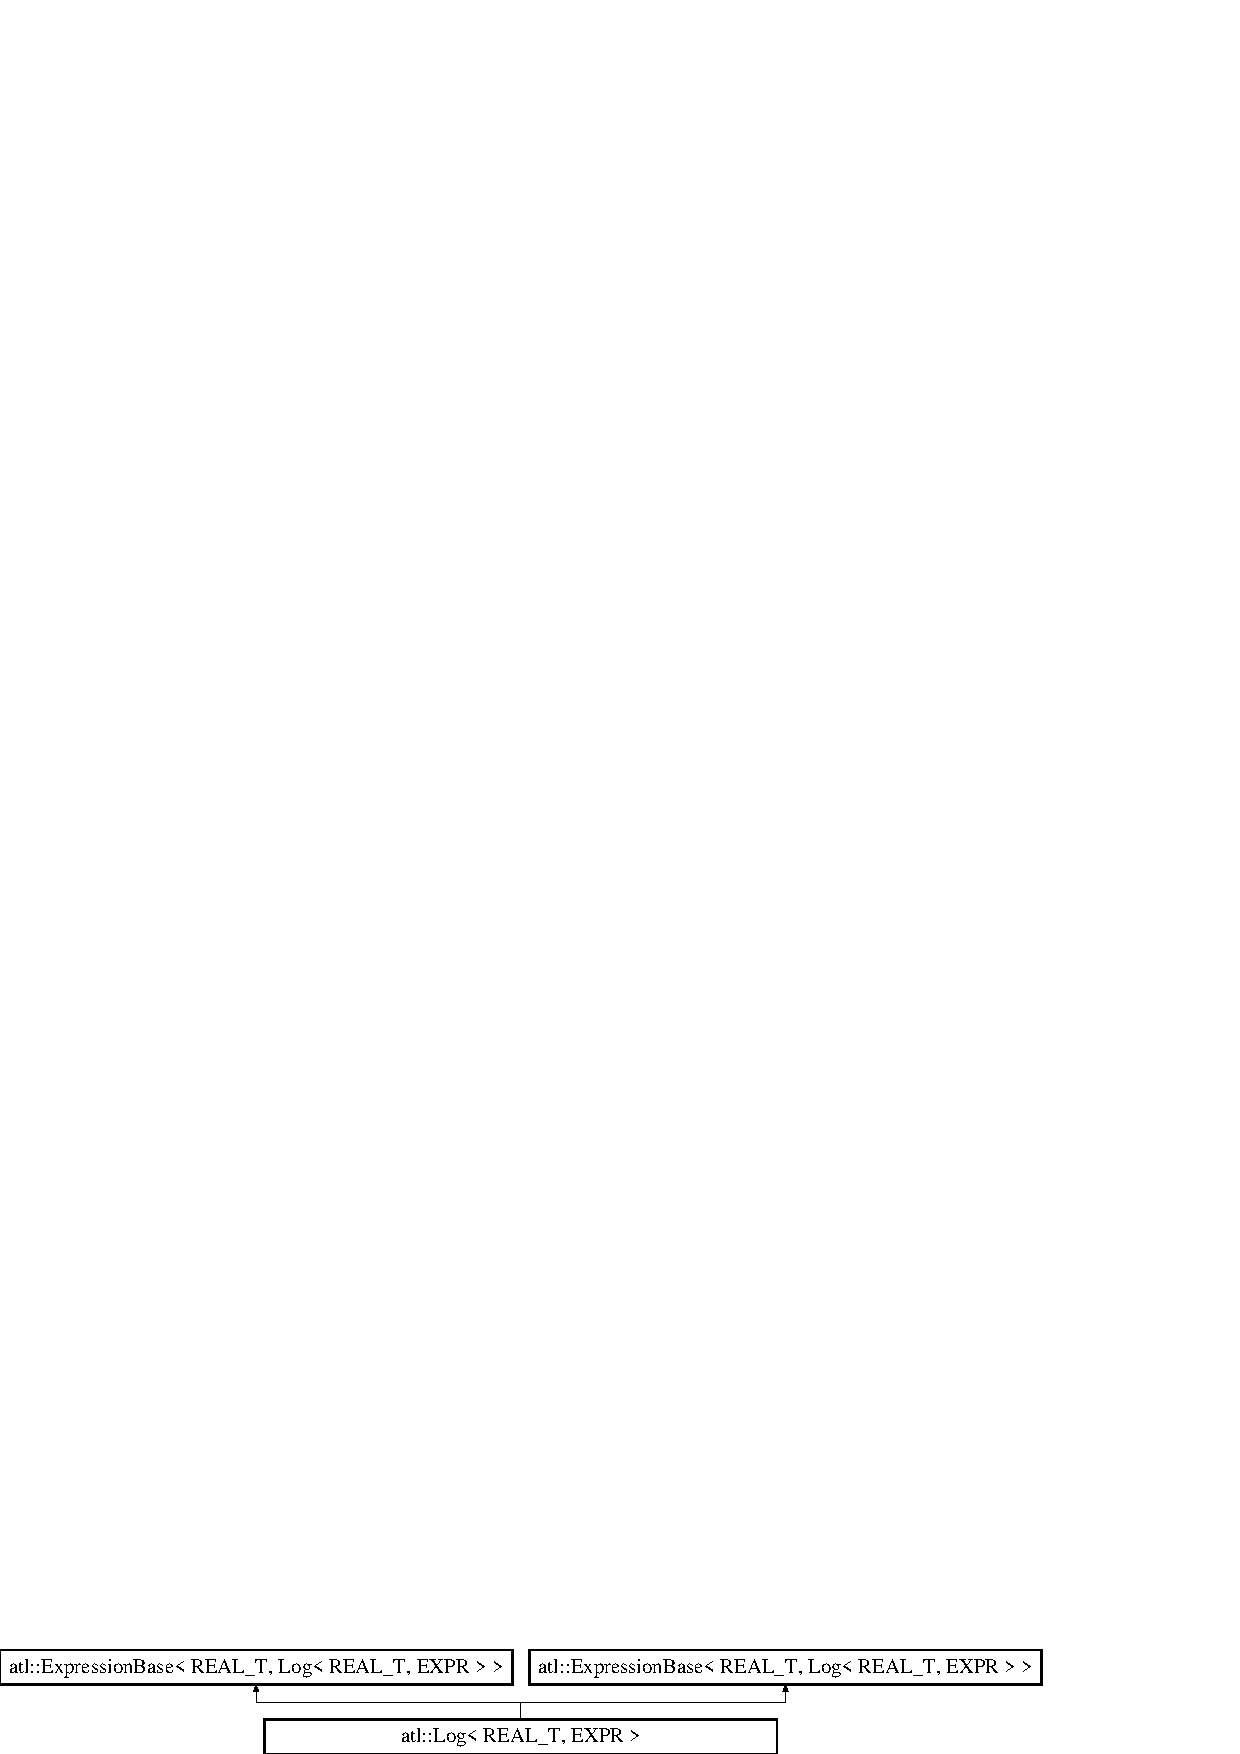
\includegraphics[height=1.642229cm]{structatl_1_1_log}
\end{center}
\end{figure}
\subsection*{Public Types}
\begin{DoxyCompactItemize}
\item 
\hypertarget{structatl_1_1_log_aa92eedd84c7f7136b0c5b609b494468e}{typedef R\+E\+A\+L\+\_\+\+T {\bfseries B\+A\+S\+E\+\_\+\+T\+Y\+P\+E}}\label{structatl_1_1_log_aa92eedd84c7f7136b0c5b609b494468e}

\item 
\hypertarget{structatl_1_1_log_aa92eedd84c7f7136b0c5b609b494468e}{typedef R\+E\+A\+L\+\_\+\+T {\bfseries B\+A\+S\+E\+\_\+\+T\+Y\+P\+E}}\label{structatl_1_1_log_aa92eedd84c7f7136b0c5b609b494468e}

\end{DoxyCompactItemize}
\subsection*{Public Member Functions}
\begin{DoxyCompactItemize}
\item 
\hypertarget{structatl_1_1_log_a01abc5bb1b4709e5fe34aa8bd568b23e}{{\bfseries Log} (const \hyperlink{structatl_1_1_expression_base}{Expression\+Base}$<$ R\+E\+A\+L\+\_\+\+T, E\+X\+P\+R $>$ \&a)}\label{structatl_1_1_log_a01abc5bb1b4709e5fe34aa8bd568b23e}

\item 
\hypertarget{structatl_1_1_log_a8af40586a9e836d67ce0ddf122992b95}{const R\+E\+A\+L\+\_\+\+T {\bfseries Get\+Value} () const }\label{structatl_1_1_log_a8af40586a9e836d67ce0ddf122992b95}

\item 
\hypertarget{structatl_1_1_log_ac6862ef00614119ee8292e4ef4d5727c}{const R\+E\+A\+L\+\_\+\+T {\bfseries Get\+Value} (size\+\_\+t i, size\+\_\+t j=0) const }\label{structatl_1_1_log_ac6862ef00614119ee8292e4ef4d5727c}

\item 
\hypertarget{structatl_1_1_log_a9b2175cc67290f3ca534d51ff1a21c39}{void {\bfseries Push\+Ids} (typename \hyperlink{structatl_1_1_stack_entry}{atl\+::\+Stack\+Entry}$<$ R\+E\+A\+L\+\_\+\+T $>$\+::vi\+\_\+storage \&ids) const }\label{structatl_1_1_log_a9b2175cc67290f3ca534d51ff1a21c39}

\item 
\hypertarget{structatl_1_1_log_ae123e08e7c97c734d3e736304f0c88ac}{void {\bfseries Push\+Ids} (typename \hyperlink{structatl_1_1_stack_entry}{atl\+::\+Stack\+Entry}$<$ R\+E\+A\+L\+\_\+\+T $>$\+::vi\+\_\+storage \&ids, size\+\_\+t i, size\+\_\+t j=0) const }\label{structatl_1_1_log_ae123e08e7c97c734d3e736304f0c88ac}

\item 
\hypertarget{structatl_1_1_log_ad0b35fedc0e0b135e1d0c18f81f69129}{const R\+E\+A\+L\+\_\+\+T {\bfseries Evaluate\+Derivative} (uint32\+\_\+t id) const }\label{structatl_1_1_log_ad0b35fedc0e0b135e1d0c18f81f69129}

\item 
\hypertarget{structatl_1_1_log_aaf20b252f35c9319c701ceeeef906c2c}{R\+E\+A\+L\+\_\+\+T {\bfseries Evaluate\+Derivative} (uint32\+\_\+t a, uint32\+\_\+t b) const }\label{structatl_1_1_log_aaf20b252f35c9319c701ceeeef906c2c}

\item 
\hypertarget{structatl_1_1_log_a2795bc68d354d69bdca6f2f2676bac21}{R\+E\+A\+L\+\_\+\+T {\bfseries Evaluate\+Derivative} (uint32\+\_\+t x, uint32\+\_\+t y, uint32\+\_\+t z) const }\label{structatl_1_1_log_a2795bc68d354d69bdca6f2f2676bac21}

\item 
\hypertarget{structatl_1_1_log_a95eaad8bfa9118c94605ff10e5321935}{const R\+E\+A\+L\+\_\+\+T {\bfseries Evaluate\+Derivative} (uint32\+\_\+t id, size\+\_\+t i, size\+\_\+t j=0) const }\label{structatl_1_1_log_a95eaad8bfa9118c94605ff10e5321935}

\item 
\hypertarget{structatl_1_1_log_a37f2c738bf455a0f9123b95aac340acd}{R\+E\+A\+L\+\_\+\+T {\bfseries Evaluate\+Derivative} (uint32\+\_\+t a, uint32\+\_\+t b, size\+\_\+t i, size\+\_\+t j=0) const }\label{structatl_1_1_log_a37f2c738bf455a0f9123b95aac340acd}

\item 
\hypertarget{structatl_1_1_log_a5afea2c7c9cabf2d692d360d16ee517f}{R\+E\+A\+L\+\_\+\+T {\bfseries Evaluate\+Derivative} (uint32\+\_\+t x, uint32\+\_\+t y, uint32\+\_\+t z, size\+\_\+t i, size\+\_\+t j=0) const }\label{structatl_1_1_log_a5afea2c7c9cabf2d692d360d16ee517f}

\item 
\hypertarget{structatl_1_1_log_a547008072cf7c797882af84e8d876e99}{size\+\_\+t {\bfseries Get\+Columns} () const }\label{structatl_1_1_log_a547008072cf7c797882af84e8d876e99}

\item 
\hypertarget{structatl_1_1_log_a417b12ff73ea48f7c88f2356d4080ea3}{size\+\_\+t {\bfseries Get\+Rows} () const }\label{structatl_1_1_log_a417b12ff73ea48f7c88f2356d4080ea3}

\item 
\hypertarget{structatl_1_1_log_adb6a4b2be4a658024101b80476a57b55}{bool {\bfseries Is\+Scalar} () const }\label{structatl_1_1_log_adb6a4b2be4a658024101b80476a57b55}

\item 
\hyperlink{structatl_1_1_log_a01abc5bb1b4709e5fe34aa8bd568b23e}{Log} (const \hyperlink{structatl_1_1_expression_base}{Expression\+Base}$<$ R\+E\+A\+L\+\_\+\+T, E\+X\+P\+R $>$ \&a)
\item 
const R\+E\+A\+L\+\_\+\+T \hyperlink{structatl_1_1_log_a8af40586a9e836d67ce0ddf122992b95}{Get\+Value} () const 
\item 
const R\+E\+A\+L\+\_\+\+T \hyperlink{structatl_1_1_log_ac6862ef00614119ee8292e4ef4d5727c}{Get\+Value} (size\+\_\+t i, size\+\_\+t j=0) const 
\item 
bool \hyperlink{structatl_1_1_log_a553838422a6da61faaafe8a4e151f6ff}{Is\+Nonlinear} () const 
\item 
void \hyperlink{structatl_1_1_log_a9b2175cc67290f3ca534d51ff1a21c39}{Push\+Ids} (typename \hyperlink{structatl_1_1_stack_entry}{atl\+::\+Stack\+Entry}$<$ R\+E\+A\+L\+\_\+\+T $>$\+::vi\+\_\+storage \&ids) const 
\item 
void \hyperlink{structatl_1_1_log_ae123e08e7c97c734d3e736304f0c88ac}{Push\+Ids} (typename \hyperlink{structatl_1_1_stack_entry}{atl\+::\+Stack\+Entry}$<$ R\+E\+A\+L\+\_\+\+T $>$\+::vi\+\_\+storage \&ids, size\+\_\+t i, size\+\_\+t j=0) const 
\item 
const R\+E\+A\+L\+\_\+\+T \hyperlink{structatl_1_1_log_a3898bf1729ca810acc0c912dbfad5e5c}{Evaluate\+Derivative} (uint32\+\_\+t x) const 
\item 
R\+E\+A\+L\+\_\+\+T \hyperlink{structatl_1_1_log_abc5371df8120d81e5f5eddec9eeaa920}{Evaluate\+Derivative} (uint32\+\_\+t x, uint32\+\_\+t y) const 
\item 
R\+E\+A\+L\+\_\+\+T \hyperlink{structatl_1_1_log_a2795bc68d354d69bdca6f2f2676bac21}{Evaluate\+Derivative} (uint32\+\_\+t x, uint32\+\_\+t y, uint32\+\_\+t z) const 
\item 
const R\+E\+A\+L\+\_\+\+T \hyperlink{structatl_1_1_log_ab1a2668eddc4e78a9d3aff7a4a5277c2}{Evaluate\+Derivative} (uint32\+\_\+t x, size\+\_\+t i, size\+\_\+t j=0) const 
\item 
R\+E\+A\+L\+\_\+\+T \hyperlink{structatl_1_1_log_a6ac182aae08d94e40a95c45e08a30303}{Evaluate\+Derivative} (uint32\+\_\+t x, uint32\+\_\+t y, size\+\_\+t i, size\+\_\+t j=0) const 
\item 
R\+E\+A\+L\+\_\+\+T \hyperlink{structatl_1_1_log_a5afea2c7c9cabf2d692d360d16ee517f}{Evaluate\+Derivative} (uint32\+\_\+t x, uint32\+\_\+t y, uint32\+\_\+t z, size\+\_\+t i, size\+\_\+t j=0) const 
\item 
size\+\_\+t \hyperlink{structatl_1_1_log_a417b12ff73ea48f7c88f2356d4080ea3}{Get\+Rows} () const 
\item 
bool \hyperlink{structatl_1_1_log_adb6a4b2be4a658024101b80476a57b55}{Is\+Scalar} () const 
\item 
const std\+::string \hyperlink{structatl_1_1_log_aba69df497f2919bec41a11d2fce6b581}{To\+Expression\+Template\+String} () const 
\end{DoxyCompactItemize}
\subsection*{Public Attributes}
\begin{DoxyCompactItemize}
\item 
\hypertarget{structatl_1_1_log_a30f64d2bdfb3951f283e7a83fe17f658}{const E\+X\+P\+R \& {\bfseries expr\+\_\+m}}\label{structatl_1_1_log_a30f64d2bdfb3951f283e7a83fe17f658}

\end{DoxyCompactItemize}


\subsection{Detailed Description}
\subsubsection*{template$<$class R\+E\+A\+L\+\_\+\+T, class E\+X\+P\+R$>$struct atl\+::\+Log$<$ R\+E\+A\+L\+\_\+\+T, E\+X\+P\+R $>$}

Expression template to handle log for variable or container expressions.

$ \log f(x,y) $

or

$ \log f_{i,j}(x,y) $ 

\subsection{Constructor \& Destructor Documentation}
\hypertarget{structatl_1_1_log_a01abc5bb1b4709e5fe34aa8bd568b23e}{\index{atl\+::\+Log@{atl\+::\+Log}!Log@{Log}}
\index{Log@{Log}!atl\+::\+Log@{atl\+::\+Log}}
\subsubsection[{Log}]{\setlength{\rightskip}{0pt plus 5cm}template$<$class R\+E\+A\+L\+\_\+\+T , class E\+X\+P\+R $>$ {\bf atl\+::\+Log}$<$ R\+E\+A\+L\+\_\+\+T, E\+X\+P\+R $>$\+::{\bf Log} (
\begin{DoxyParamCaption}
\item[{const {\bf Expression\+Base}$<$ R\+E\+A\+L\+\_\+\+T, E\+X\+P\+R $>$ \&}]{a}
\end{DoxyParamCaption}
)\hspace{0.3cm}{\ttfamily [inline]}}}\label{structatl_1_1_log_a01abc5bb1b4709e5fe34aa8bd568b23e}
Constructor


\begin{DoxyParams}{Parameters}
{\em a} & \\
\hline
\end{DoxyParams}


\subsection{Member Function Documentation}
\hypertarget{structatl_1_1_log_a3898bf1729ca810acc0c912dbfad5e5c}{\index{atl\+::\+Log@{atl\+::\+Log}!Evaluate\+Derivative@{Evaluate\+Derivative}}
\index{Evaluate\+Derivative@{Evaluate\+Derivative}!atl\+::\+Log@{atl\+::\+Log}}
\subsubsection[{Evaluate\+Derivative}]{\setlength{\rightskip}{0pt plus 5cm}template$<$class R\+E\+A\+L\+\_\+\+T , class E\+X\+P\+R $>$ const R\+E\+A\+L\+\_\+\+T {\bf atl\+::\+Log}$<$ R\+E\+A\+L\+\_\+\+T, E\+X\+P\+R $>$\+::Evaluate\+Derivative (
\begin{DoxyParamCaption}
\item[{uint32\+\_\+t}]{x}
\end{DoxyParamCaption}
) const\hspace{0.3cm}{\ttfamily [inline]}}}\label{structatl_1_1_log_a3898bf1729ca810acc0c912dbfad5e5c}
Evaluates the first-\/order derivative with respect to x.

$ {{{{d}\over{d\,x}}\,f_{i,j}(x)}\over{f_{i,j}(x)}} $


\begin{DoxyParams}{Parameters}
{\em x} & \\
\hline
\end{DoxyParams}
\begin{DoxyReturn}{Returns}

\end{DoxyReturn}
\hypertarget{structatl_1_1_log_abc5371df8120d81e5f5eddec9eeaa920}{\index{atl\+::\+Log@{atl\+::\+Log}!Evaluate\+Derivative@{Evaluate\+Derivative}}
\index{Evaluate\+Derivative@{Evaluate\+Derivative}!atl\+::\+Log@{atl\+::\+Log}}
\subsubsection[{Evaluate\+Derivative}]{\setlength{\rightskip}{0pt plus 5cm}template$<$class R\+E\+A\+L\+\_\+\+T , class E\+X\+P\+R $>$ R\+E\+A\+L\+\_\+\+T {\bf atl\+::\+Log}$<$ R\+E\+A\+L\+\_\+\+T, E\+X\+P\+R $>$\+::Evaluate\+Derivative (
\begin{DoxyParamCaption}
\item[{uint32\+\_\+t}]{x, }
\item[{uint32\+\_\+t}]{y}
\end{DoxyParamCaption}
) const\hspace{0.3cm}{\ttfamily [inline]}}}\label{structatl_1_1_log_abc5371df8120d81e5f5eddec9eeaa920}
Evaluates the second-\/order derivative with respect to x and y.

$ {{{{d^2}\over{d\,x\,d\,y}}\,f(x,y)}\over{f(x,y)}}-{{{{d }\over{d\,x}}\,f(x,y)\,\left({{d}\over{d\,y}}\,f(x,y) \right)}\over{f(x,y)^2}} $


\begin{DoxyParams}{Parameters}
{\em x} & \\
\hline
{\em y} & \\
\hline
\end{DoxyParams}
\begin{DoxyReturn}{Returns}

\end{DoxyReturn}
\hypertarget{structatl_1_1_log_a2795bc68d354d69bdca6f2f2676bac21}{\index{atl\+::\+Log@{atl\+::\+Log}!Evaluate\+Derivative@{Evaluate\+Derivative}}
\index{Evaluate\+Derivative@{Evaluate\+Derivative}!atl\+::\+Log@{atl\+::\+Log}}
\subsubsection[{Evaluate\+Derivative}]{\setlength{\rightskip}{0pt plus 5cm}template$<$class R\+E\+A\+L\+\_\+\+T , class E\+X\+P\+R $>$ R\+E\+A\+L\+\_\+\+T {\bf atl\+::\+Log}$<$ R\+E\+A\+L\+\_\+\+T, E\+X\+P\+R $>$\+::Evaluate\+Derivative (
\begin{DoxyParamCaption}
\item[{uint32\+\_\+t}]{x, }
\item[{uint32\+\_\+t}]{y, }
\item[{uint32\+\_\+t}]{z}
\end{DoxyParamCaption}
) const\hspace{0.3cm}{\ttfamily [inline]}}}\label{structatl_1_1_log_a2795bc68d354d69bdca6f2f2676bac21}
Evaluates the third-\/order derivative with respect to x, y, and z.

$ {{2\,\left({{d}\over{d\,x}}\,f(x,y,z)\right)\,\left({{d }\over{d\,y}}\,f(x,y,z)\right)\,\left({{d}\over{d\,z}}\,f_{i,j }(x,y,z)\right)}\over{f(x,y,z)^3}}-{{{{d^2}\over{d\,x\,d\,y}} \,f(x,y,z)\,\left({{d}\over{d\,z}}\,f(x,y,z)\right) }\over{f(x,y,z)^2}}-{{{{d}\over{d\,x}}\,f(x,y,z)\,\left( {{d^2}\over{d\,y\,d\,z}}\,f(x,y,z)\right)}\over{f(x,y,z) ^2}}-{{{{d^2}\over{d\,x\,d\,z}}\,f(x,y,z)\,\left({{d}\over{d\, y}}\,f(x,y,z)\right)}\over{f(x,y,z)^2}}+{{{{d^3}\over{d \,x\,d\,y\,d\,z}}\,f(x,y,z)}\over{f(x,y,z)}} $


\begin{DoxyParams}{Parameters}
{\em x} & \\
\hline
{\em y} & \\
\hline
{\em z} & \\
\hline
\end{DoxyParams}
\begin{DoxyReturn}{Returns}

\end{DoxyReturn}
\hypertarget{structatl_1_1_log_ab1a2668eddc4e78a9d3aff7a4a5277c2}{\index{atl\+::\+Log@{atl\+::\+Log}!Evaluate\+Derivative@{Evaluate\+Derivative}}
\index{Evaluate\+Derivative@{Evaluate\+Derivative}!atl\+::\+Log@{atl\+::\+Log}}
\subsubsection[{Evaluate\+Derivative}]{\setlength{\rightskip}{0pt plus 5cm}template$<$class R\+E\+A\+L\+\_\+\+T , class E\+X\+P\+R $>$ const R\+E\+A\+L\+\_\+\+T {\bf atl\+::\+Log}$<$ R\+E\+A\+L\+\_\+\+T, E\+X\+P\+R $>$\+::Evaluate\+Derivative (
\begin{DoxyParamCaption}
\item[{uint32\+\_\+t}]{x, }
\item[{size\+\_\+t}]{i, }
\item[{size\+\_\+t}]{j = {\ttfamily 0}}
\end{DoxyParamCaption}
) const\hspace{0.3cm}{\ttfamily [inline]}}}\label{structatl_1_1_log_ab1a2668eddc4e78a9d3aff7a4a5277c2}
Evaluates the first-\/order derivative with respect to x at index \{i,j\}.

$ {{{{d}\over{d\,x}}\,f_{i,j}(x)}\over{f_{i,j}(x)}} $


\begin{DoxyParams}{Parameters}
{\em x} & \\
\hline
{\em i} & \\
\hline
{\em j} & \\
\hline
\end{DoxyParams}
\begin{DoxyReturn}{Returns}

\end{DoxyReturn}
\hypertarget{structatl_1_1_log_a6ac182aae08d94e40a95c45e08a30303}{\index{atl\+::\+Log@{atl\+::\+Log}!Evaluate\+Derivative@{Evaluate\+Derivative}}
\index{Evaluate\+Derivative@{Evaluate\+Derivative}!atl\+::\+Log@{atl\+::\+Log}}
\subsubsection[{Evaluate\+Derivative}]{\setlength{\rightskip}{0pt plus 5cm}template$<$class R\+E\+A\+L\+\_\+\+T , class E\+X\+P\+R $>$ R\+E\+A\+L\+\_\+\+T {\bf atl\+::\+Log}$<$ R\+E\+A\+L\+\_\+\+T, E\+X\+P\+R $>$\+::Evaluate\+Derivative (
\begin{DoxyParamCaption}
\item[{uint32\+\_\+t}]{x, }
\item[{uint32\+\_\+t}]{y, }
\item[{size\+\_\+t}]{i, }
\item[{size\+\_\+t}]{j = {\ttfamily 0}}
\end{DoxyParamCaption}
) const\hspace{0.3cm}{\ttfamily [inline]}}}\label{structatl_1_1_log_a6ac182aae08d94e40a95c45e08a30303}
Evaluates the second-\/order derivative with respect to x and y at index \{i,j\}.

$ {{{{d^2}\over{d\,x\,d\,y}}\,f_{i,j}(x,y)}\over{f_{i,j}(x,y)}}-{{{{d }\over{d\,x}}\,f_{i,j}(x,y)\,\left({{d}\over{d\,y}}\,f_{i,j}(x,y) \right)}\over{f_{i,j}(x,y)^2}} $


\begin{DoxyParams}{Parameters}
{\em x} & \\
\hline
{\em y} & \\
\hline
{\em i} & \\
\hline
{\em j} & \\
\hline
\end{DoxyParams}
\begin{DoxyReturn}{Returns}

\end{DoxyReturn}
\hypertarget{structatl_1_1_log_a5afea2c7c9cabf2d692d360d16ee517f}{\index{atl\+::\+Log@{atl\+::\+Log}!Evaluate\+Derivative@{Evaluate\+Derivative}}
\index{Evaluate\+Derivative@{Evaluate\+Derivative}!atl\+::\+Log@{atl\+::\+Log}}
\subsubsection[{Evaluate\+Derivative}]{\setlength{\rightskip}{0pt plus 5cm}template$<$class R\+E\+A\+L\+\_\+\+T , class E\+X\+P\+R $>$ R\+E\+A\+L\+\_\+\+T {\bf atl\+::\+Log}$<$ R\+E\+A\+L\+\_\+\+T, E\+X\+P\+R $>$\+::Evaluate\+Derivative (
\begin{DoxyParamCaption}
\item[{uint32\+\_\+t}]{x, }
\item[{uint32\+\_\+t}]{y, }
\item[{uint32\+\_\+t}]{z, }
\item[{size\+\_\+t}]{i, }
\item[{size\+\_\+t}]{j = {\ttfamily 0}}
\end{DoxyParamCaption}
) const\hspace{0.3cm}{\ttfamily [inline]}}}\label{structatl_1_1_log_a5afea2c7c9cabf2d692d360d16ee517f}
Evaluates the third-\/order derivative with respect to x, y, and z at index \{i,j\}.

$ {{2\,\left({{d}\over{d\,x}}\,f_{i,j}(x,y,z)\right)\,\left({{d }\over{d\,y}}\,f_{i,j}(x,y,z)\right)\,\left({{d}\over{d\,z}}\,f_{i,j }(x,y,z)\right)}\over{f_{i,j}(x,y,z)^3}}-{{{{d^2}\over{d\,x\,d\,y}} \,f_{i,j}(x,y,z)\,\left({{d}\over{d\,z}}\,f_{i,j}(x,y,z)\right) }\over{f_{i,j}(x,y,z)^2}}-{{{{d}\over{d\,x}}\,f_{i,j}(x,y,z)\,\left( {{d^2}\over{d\,y\,d\,z}}\,f_{i,j}(x,y,z)\right)}\over{f_{i,j}(x,y,z) ^2}}-{{{{d^2}\over{d\,x\,d\,z}}\,f_{i,j}(x,y,z)\,\left({{d}\over{d\, y}}\,f_{i,j}(x,y,z)\right)}\over{f_{i,j}(x,y,z)^2}}+{{{{d^3}\over{d \,x\,d\,y\,d\,z}}\,f_{i,j}(x,y,z)}\over{f_{i,j}(x,y,z)}} $


\begin{DoxyParams}{Parameters}
{\em x} & \\
\hline
{\em y} & \\
\hline
{\em z} & \\
\hline
{\em i} & \\
\hline
{\em j} & \\
\hline
\end{DoxyParams}
\begin{DoxyReturn}{Returns}

\end{DoxyReturn}
\hypertarget{structatl_1_1_log_a417b12ff73ea48f7c88f2356d4080ea3}{\index{atl\+::\+Log@{atl\+::\+Log}!Get\+Rows@{Get\+Rows}}
\index{Get\+Rows@{Get\+Rows}!atl\+::\+Log@{atl\+::\+Log}}
\subsubsection[{Get\+Rows}]{\setlength{\rightskip}{0pt plus 5cm}template$<$class R\+E\+A\+L\+\_\+\+T , class E\+X\+P\+R $>$ size\+\_\+t {\bf atl\+::\+Log}$<$ R\+E\+A\+L\+\_\+\+T, E\+X\+P\+R $>$\+::Get\+Rows (
\begin{DoxyParamCaption}
{}
\end{DoxyParamCaption}
) const\hspace{0.3cm}{\ttfamily [inline]}}}\label{structatl_1_1_log_a417b12ff73ea48f7c88f2356d4080ea3}
Return the number of rows.

\begin{DoxyReturn}{Returns}

\end{DoxyReturn}
\hypertarget{structatl_1_1_log_a8af40586a9e836d67ce0ddf122992b95}{\index{atl\+::\+Log@{atl\+::\+Log}!Get\+Value@{Get\+Value}}
\index{Get\+Value@{Get\+Value}!atl\+::\+Log@{atl\+::\+Log}}
\subsubsection[{Get\+Value}]{\setlength{\rightskip}{0pt plus 5cm}template$<$class R\+E\+A\+L\+\_\+\+T , class E\+X\+P\+R $>$ const R\+E\+A\+L\+\_\+\+T {\bf atl\+::\+Log}$<$ R\+E\+A\+L\+\_\+\+T, E\+X\+P\+R $>$\+::Get\+Value (
\begin{DoxyParamCaption}
{}
\end{DoxyParamCaption}
) const\hspace{0.3cm}{\ttfamily [inline]}}}\label{structatl_1_1_log_a8af40586a9e836d67ce0ddf122992b95}
Computes the log of the evaluated expression.

\begin{DoxyReturn}{Returns}

\end{DoxyReturn}
\hypertarget{structatl_1_1_log_ac6862ef00614119ee8292e4ef4d5727c}{\index{atl\+::\+Log@{atl\+::\+Log}!Get\+Value@{Get\+Value}}
\index{Get\+Value@{Get\+Value}!atl\+::\+Log@{atl\+::\+Log}}
\subsubsection[{Get\+Value}]{\setlength{\rightskip}{0pt plus 5cm}template$<$class R\+E\+A\+L\+\_\+\+T , class E\+X\+P\+R $>$ const R\+E\+A\+L\+\_\+\+T {\bf atl\+::\+Log}$<$ R\+E\+A\+L\+\_\+\+T, E\+X\+P\+R $>$\+::Get\+Value (
\begin{DoxyParamCaption}
\item[{size\+\_\+t}]{i, }
\item[{size\+\_\+t}]{j = {\ttfamily 0}}
\end{DoxyParamCaption}
) const\hspace{0.3cm}{\ttfamily [inline]}}}\label{structatl_1_1_log_ac6862ef00614119ee8292e4ef4d5727c}
Computes the log of the evaluated expression at index \{i,j\}.


\begin{DoxyParams}{Parameters}
{\em i} & \\
\hline
{\em j} & \\
\hline
\end{DoxyParams}
\begin{DoxyReturn}{Returns}

\end{DoxyReturn}
\hypertarget{structatl_1_1_log_a553838422a6da61faaafe8a4e151f6ff}{\index{atl\+::\+Log@{atl\+::\+Log}!Is\+Nonlinear@{Is\+Nonlinear}}
\index{Is\+Nonlinear@{Is\+Nonlinear}!atl\+::\+Log@{atl\+::\+Log}}
\subsubsection[{Is\+Nonlinear}]{\setlength{\rightskip}{0pt plus 5cm}template$<$class R\+E\+A\+L\+\_\+\+T , class E\+X\+P\+R $>$ bool {\bf atl\+::\+Log}$<$ R\+E\+A\+L\+\_\+\+T, E\+X\+P\+R $>$\+::Is\+Nonlinear (
\begin{DoxyParamCaption}
{}
\end{DoxyParamCaption}
) const\hspace{0.3cm}{\ttfamily [inline]}}}\label{structatl_1_1_log_a553838422a6da61faaafe8a4e151f6ff}
Returns true.

\begin{DoxyReturn}{Returns}

\end{DoxyReturn}
\hypertarget{structatl_1_1_log_adb6a4b2be4a658024101b80476a57b55}{\index{atl\+::\+Log@{atl\+::\+Log}!Is\+Scalar@{Is\+Scalar}}
\index{Is\+Scalar@{Is\+Scalar}!atl\+::\+Log@{atl\+::\+Log}}
\subsubsection[{Is\+Scalar}]{\setlength{\rightskip}{0pt plus 5cm}template$<$class R\+E\+A\+L\+\_\+\+T , class E\+X\+P\+R $>$ bool {\bf atl\+::\+Log}$<$ R\+E\+A\+L\+\_\+\+T, E\+X\+P\+R $>$\+::Is\+Scalar (
\begin{DoxyParamCaption}
{}
\end{DoxyParamCaption}
) const\hspace{0.3cm}{\ttfamily [inline]}}}\label{structatl_1_1_log_adb6a4b2be4a658024101b80476a57b55}
True if this expression is a scalar.

\begin{DoxyReturn}{Returns}

\end{DoxyReturn}
\hypertarget{structatl_1_1_log_a9b2175cc67290f3ca534d51ff1a21c39}{\index{atl\+::\+Log@{atl\+::\+Log}!Push\+Ids@{Push\+Ids}}
\index{Push\+Ids@{Push\+Ids}!atl\+::\+Log@{atl\+::\+Log}}
\subsubsection[{Push\+Ids}]{\setlength{\rightskip}{0pt plus 5cm}template$<$class R\+E\+A\+L\+\_\+\+T , class E\+X\+P\+R $>$ void {\bf atl\+::\+Log}$<$ R\+E\+A\+L\+\_\+\+T, E\+X\+P\+R $>$\+::Push\+Ids (
\begin{DoxyParamCaption}
\item[{typename {\bf atl\+::\+Stack\+Entry}$<$ R\+E\+A\+L\+\_\+\+T $>$\+::vi\+\_\+storage \&}]{ids}
\end{DoxyParamCaption}
) const\hspace{0.3cm}{\ttfamily [inline]}}}\label{structatl_1_1_log_a9b2175cc67290f3ca534d51ff1a21c39}
Push variable info into a set.


\begin{DoxyParams}{Parameters}
{\em ids} & \\
\hline
\end{DoxyParams}
\hypertarget{structatl_1_1_log_ae123e08e7c97c734d3e736304f0c88ac}{\index{atl\+::\+Log@{atl\+::\+Log}!Push\+Ids@{Push\+Ids}}
\index{Push\+Ids@{Push\+Ids}!atl\+::\+Log@{atl\+::\+Log}}
\subsubsection[{Push\+Ids}]{\setlength{\rightskip}{0pt plus 5cm}template$<$class R\+E\+A\+L\+\_\+\+T , class E\+X\+P\+R $>$ void {\bf atl\+::\+Log}$<$ R\+E\+A\+L\+\_\+\+T, E\+X\+P\+R $>$\+::Push\+Ids (
\begin{DoxyParamCaption}
\item[{typename {\bf atl\+::\+Stack\+Entry}$<$ R\+E\+A\+L\+\_\+\+T $>$\+::vi\+\_\+storage \&}]{ids, }
\item[{size\+\_\+t}]{i, }
\item[{size\+\_\+t}]{j = {\ttfamily 0}}
\end{DoxyParamCaption}
) const\hspace{0.3cm}{\ttfamily [inline]}}}\label{structatl_1_1_log_ae123e08e7c97c734d3e736304f0c88ac}
Push variable info into a set at index \{i,j\}.


\begin{DoxyParams}{Parameters}
{\em ids} & \\
\hline
{\em i} & \\
\hline
{\em j} & \\
\hline
\end{DoxyParams}
\hypertarget{structatl_1_1_log_aba69df497f2919bec41a11d2fce6b581}{\index{atl\+::\+Log@{atl\+::\+Log}!To\+Expression\+Template\+String@{To\+Expression\+Template\+String}}
\index{To\+Expression\+Template\+String@{To\+Expression\+Template\+String}!atl\+::\+Log@{atl\+::\+Log}}
\subsubsection[{To\+Expression\+Template\+String}]{\setlength{\rightskip}{0pt plus 5cm}template$<$class R\+E\+A\+L\+\_\+\+T , class E\+X\+P\+R $>$ const std\+::string {\bf atl\+::\+Log}$<$ R\+E\+A\+L\+\_\+\+T, E\+X\+P\+R $>$\+::To\+Expression\+Template\+String (
\begin{DoxyParamCaption}
{}
\end{DoxyParamCaption}
) const\hspace{0.3cm}{\ttfamily [inline]}}}\label{structatl_1_1_log_aba69df497f2919bec41a11d2fce6b581}
Create a string representation of this expression template. \begin{DoxyReturn}{Returns}

\end{DoxyReturn}


The documentation for this struct was generated from the following file\+:\begin{DoxyCompactItemize}
\item 
A\+T\+L2/Log.\+hpp\end{DoxyCompactItemize}

\hypertarget{structatl_1_1_log10}{\section{atl\+:\+:Log10$<$ R\+E\+A\+L\+\_\+\+T, E\+X\+P\+R $>$ Struct Template Reference}
\label{structatl_1_1_log10}\index{atl\+::\+Log10$<$ R\+E\+A\+L\+\_\+\+T, E\+X\+P\+R $>$@{atl\+::\+Log10$<$ R\+E\+A\+L\+\_\+\+T, E\+X\+P\+R $>$}}
}


{\ttfamily \#include $<$Log10.\+hpp$>$}

Inheritance diagram for atl\+:\+:Log10$<$ R\+E\+A\+L\+\_\+\+T, E\+X\+P\+R $>$\+:\begin{figure}[H]
\begin{center}
\leavevmode
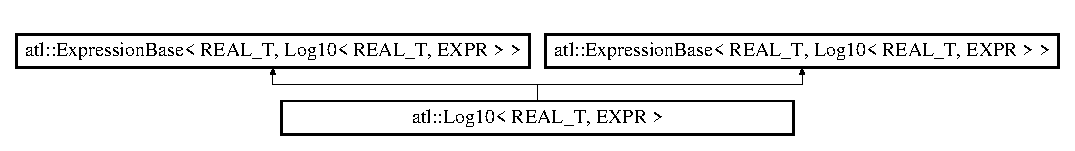
\includegraphics[height=1.577465cm]{structatl_1_1_log10}
\end{center}
\end{figure}
\subsection*{Public Types}
\begin{DoxyCompactItemize}
\item 
\hypertarget{structatl_1_1_log10_ac314523300a5d801ea0605e6df1cbdc4}{typedef R\+E\+A\+L\+\_\+\+T {\bfseries B\+A\+S\+E\+\_\+\+T\+Y\+P\+E}}\label{structatl_1_1_log10_ac314523300a5d801ea0605e6df1cbdc4}

\item 
\hypertarget{structatl_1_1_log10_ac314523300a5d801ea0605e6df1cbdc4}{typedef R\+E\+A\+L\+\_\+\+T {\bfseries B\+A\+S\+E\+\_\+\+T\+Y\+P\+E}}\label{structatl_1_1_log10_ac314523300a5d801ea0605e6df1cbdc4}

\end{DoxyCompactItemize}
\subsection*{Public Member Functions}
\begin{DoxyCompactItemize}
\item 
\hypertarget{structatl_1_1_log10_a179bd24f45cb40d8c4c69b399d9ab006}{{\bfseries Log10} (const \hyperlink{structatl_1_1_expression_base}{Expression\+Base}$<$ R\+E\+A\+L\+\_\+\+T, E\+X\+P\+R $>$ \&a)}\label{structatl_1_1_log10_a179bd24f45cb40d8c4c69b399d9ab006}

\item 
\hypertarget{structatl_1_1_log10_a4ef8c45dadaf5851b95dad741f797744}{const R\+E\+A\+L\+\_\+\+T {\bfseries Get\+Value} () const }\label{structatl_1_1_log10_a4ef8c45dadaf5851b95dad741f797744}

\item 
\hypertarget{structatl_1_1_log10_af6ddeb7607474a178aef69daf1cecc6d}{const R\+E\+A\+L\+\_\+\+T {\bfseries Get\+Value} (size\+\_\+t i, size\+\_\+t j=0) const }\label{structatl_1_1_log10_af6ddeb7607474a178aef69daf1cecc6d}

\item 
\hypertarget{structatl_1_1_log10_ada7fc1f52b2b6f91260e01835c368158}{void {\bfseries Push\+Ids} (typename \hyperlink{structatl_1_1_stack_entry}{atl\+::\+Stack\+Entry}$<$ R\+E\+A\+L\+\_\+\+T $>$\+::vi\+\_\+storage \&ids) const }\label{structatl_1_1_log10_ada7fc1f52b2b6f91260e01835c368158}

\item 
\hypertarget{structatl_1_1_log10_afa4734b1fa8a2f019607387bd9c397c2}{void {\bfseries Push\+Ids} (typename \hyperlink{structatl_1_1_stack_entry}{atl\+::\+Stack\+Entry}$<$ R\+E\+A\+L\+\_\+\+T $>$\+::vi\+\_\+storage \&ids, size\+\_\+t i, size\+\_\+t j=0) const }\label{structatl_1_1_log10_afa4734b1fa8a2f019607387bd9c397c2}

\item 
\hypertarget{structatl_1_1_log10_a4e6b29b6764fe0563aa483f3e552bf95}{const R\+E\+A\+L\+\_\+\+T {\bfseries Evaluate\+Derivative} (uint32\+\_\+t id) const }\label{structatl_1_1_log10_a4e6b29b6764fe0563aa483f3e552bf95}

\item 
\hypertarget{structatl_1_1_log10_a852de4fd2d8456c84ca4d923f97886a4}{R\+E\+A\+L\+\_\+\+T {\bfseries Evaluate\+Derivative} (uint32\+\_\+t a, uint32\+\_\+t b) const }\label{structatl_1_1_log10_a852de4fd2d8456c84ca4d923f97886a4}

\item 
\hypertarget{structatl_1_1_log10_aac9a5699adc29f8abb687400f6b1781f}{R\+E\+A\+L\+\_\+\+T {\bfseries Evaluate\+Derivative} (uint32\+\_\+t x, uint32\+\_\+t y, uint32\+\_\+t z) const }\label{structatl_1_1_log10_aac9a5699adc29f8abb687400f6b1781f}

\item 
\hypertarget{structatl_1_1_log10_af2134f46d9d89c6902db5395bcb94380}{const R\+E\+A\+L\+\_\+\+T {\bfseries Evaluate\+Derivative} (uint32\+\_\+t id, size\+\_\+t i, size\+\_\+t j=0) const }\label{structatl_1_1_log10_af2134f46d9d89c6902db5395bcb94380}

\item 
\hypertarget{structatl_1_1_log10_a2418f82c3a40624656a78e278c3567d6}{R\+E\+A\+L\+\_\+\+T {\bfseries Evaluate\+Derivative} (uint32\+\_\+t a, uint32\+\_\+t b, size\+\_\+t i, size\+\_\+t j=0) const }\label{structatl_1_1_log10_a2418f82c3a40624656a78e278c3567d6}

\item 
\hypertarget{structatl_1_1_log10_aa026f9fc6efae054e531442c61207951}{R\+E\+A\+L\+\_\+\+T {\bfseries Evaluate\+Derivative} (uint32\+\_\+t x, uint32\+\_\+t y, uint32\+\_\+t z, size\+\_\+t i, size\+\_\+t j=0) const }\label{structatl_1_1_log10_aa026f9fc6efae054e531442c61207951}

\item 
\hypertarget{structatl_1_1_log10_a8b5f8aa7512a7d157810b4d11e8f6f5e}{size\+\_\+t {\bfseries Get\+Columns} () const }\label{structatl_1_1_log10_a8b5f8aa7512a7d157810b4d11e8f6f5e}

\item 
\hypertarget{structatl_1_1_log10_ac84945c7c8f62c7333cbda7b9044bfc4}{size\+\_\+t {\bfseries Get\+Rows} () const }\label{structatl_1_1_log10_ac84945c7c8f62c7333cbda7b9044bfc4}

\item 
\hypertarget{structatl_1_1_log10_afc6637bc3430acc84043298ff4f084ba}{bool {\bfseries Is\+Scalar} () const }\label{structatl_1_1_log10_afc6637bc3430acc84043298ff4f084ba}

\item 
\hyperlink{structatl_1_1_log10_a179bd24f45cb40d8c4c69b399d9ab006}{Log10} (const \hyperlink{structatl_1_1_expression_base}{Expression\+Base}$<$ R\+E\+A\+L\+\_\+\+T, E\+X\+P\+R $>$ \&a)
\item 
const R\+E\+A\+L\+\_\+\+T \hyperlink{structatl_1_1_log10_a4ef8c45dadaf5851b95dad741f797744}{Get\+Value} () const 
\item 
const R\+E\+A\+L\+\_\+\+T \hyperlink{structatl_1_1_log10_af6ddeb7607474a178aef69daf1cecc6d}{Get\+Value} (size\+\_\+t i, size\+\_\+t j=0) const 
\item 
bool \hyperlink{structatl_1_1_log10_a35042523fd50670b38c932f65f165660}{Is\+Nonlinear} () const 
\item 
void \hyperlink{structatl_1_1_log10_ada7fc1f52b2b6f91260e01835c368158}{Push\+Ids} (typename \hyperlink{structatl_1_1_stack_entry}{atl\+::\+Stack\+Entry}$<$ R\+E\+A\+L\+\_\+\+T $>$\+::vi\+\_\+storage \&ids) const 
\item 
void \hyperlink{structatl_1_1_log10_afa4734b1fa8a2f019607387bd9c397c2}{Push\+Ids} (typename \hyperlink{structatl_1_1_stack_entry}{atl\+::\+Stack\+Entry}$<$ R\+E\+A\+L\+\_\+\+T $>$\+::vi\+\_\+storage \&ids, size\+\_\+t i, size\+\_\+t j=0) const 
\item 
const R\+E\+A\+L\+\_\+\+T \hyperlink{structatl_1_1_log10_a1a8d53a7ee75d5b4e7e23821df097bf3}{Evaluate\+Derivative} (uint32\+\_\+t x) const 
\item 
R\+E\+A\+L\+\_\+\+T \hyperlink{structatl_1_1_log10_a2551cc893bd6d4e0bb4c3e8da3767696}{Evaluate\+Derivative} (uint32\+\_\+t x, uint32\+\_\+t y) const 
\item 
R\+E\+A\+L\+\_\+\+T \hyperlink{structatl_1_1_log10_aac9a5699adc29f8abb687400f6b1781f}{Evaluate\+Derivative} (uint32\+\_\+t x, uint32\+\_\+t y, uint32\+\_\+t z) const 
\item 
const R\+E\+A\+L\+\_\+\+T \hyperlink{structatl_1_1_log10_ae24fe26a0bbed5c9099ce91cec6e0252}{Evaluate\+Derivative} (uint32\+\_\+t x, size\+\_\+t i, size\+\_\+t j=0) const 
\item 
R\+E\+A\+L\+\_\+\+T \hyperlink{structatl_1_1_log10_a4f85bc4ecebbc205a5784ae1a67f574c}{Evaluate\+Derivative} (uint32\+\_\+t x, uint32\+\_\+t y, size\+\_\+t i, size\+\_\+t j=0) const 
\item 
R\+E\+A\+L\+\_\+\+T \hyperlink{structatl_1_1_log10_aa026f9fc6efae054e531442c61207951}{Evaluate\+Derivative} (uint32\+\_\+t x, uint32\+\_\+t y, uint32\+\_\+t z, size\+\_\+t i, size\+\_\+t j=0) const 
\item 
size\+\_\+t \hyperlink{structatl_1_1_log10_ac84945c7c8f62c7333cbda7b9044bfc4}{Get\+Rows} () const 
\item 
bool \hyperlink{structatl_1_1_log10_afc6637bc3430acc84043298ff4f084ba}{Is\+Scalar} () const 
\item 
const std\+::string \hyperlink{structatl_1_1_log10_a220c67729ae6c659e824378a97d110d6}{To\+Expression\+Template\+String} () const 
\end{DoxyCompactItemize}
\subsection*{Public Attributes}
\begin{DoxyCompactItemize}
\item 
\hypertarget{structatl_1_1_log10_a5c6029ad779bc4004eb63d329f4357fb}{const E\+X\+P\+R \& {\bfseries expr\+\_\+m}}\label{structatl_1_1_log10_a5c6029ad779bc4004eb63d329f4357fb}

\end{DoxyCompactItemize}


\subsection{Detailed Description}
\subsubsection*{template$<$class R\+E\+A\+L\+\_\+\+T, class E\+X\+P\+R$>$struct atl\+::\+Log10$<$ R\+E\+A\+L\+\_\+\+T, E\+X\+P\+R $>$}

Expression template to handle log10 for variable or container expressions.

$ {\it log_{10}}\left(f(x)\right) $

or

$ {\it log_{10}}\left(f_{i,j}(x)\right) $ 

\subsection{Constructor \& Destructor Documentation}
\hypertarget{structatl_1_1_log10_a179bd24f45cb40d8c4c69b399d9ab006}{\index{atl\+::\+Log10@{atl\+::\+Log10}!Log10@{Log10}}
\index{Log10@{Log10}!atl\+::\+Log10@{atl\+::\+Log10}}
\subsubsection[{Log10}]{\setlength{\rightskip}{0pt plus 5cm}template$<$class R\+E\+A\+L\+\_\+\+T , class E\+X\+P\+R $>$ {\bf atl\+::\+Log10}$<$ R\+E\+A\+L\+\_\+\+T, E\+X\+P\+R $>$\+::{\bf Log10} (
\begin{DoxyParamCaption}
\item[{const {\bf Expression\+Base}$<$ R\+E\+A\+L\+\_\+\+T, E\+X\+P\+R $>$ \&}]{a}
\end{DoxyParamCaption}
)\hspace{0.3cm}{\ttfamily [inline]}}}\label{structatl_1_1_log10_a179bd24f45cb40d8c4c69b399d9ab006}
Constructor


\begin{DoxyParams}{Parameters}
{\em a} & \\
\hline
\end{DoxyParams}


\subsection{Member Function Documentation}
\hypertarget{structatl_1_1_log10_a1a8d53a7ee75d5b4e7e23821df097bf3}{\index{atl\+::\+Log10@{atl\+::\+Log10}!Evaluate\+Derivative@{Evaluate\+Derivative}}
\index{Evaluate\+Derivative@{Evaluate\+Derivative}!atl\+::\+Log10@{atl\+::\+Log10}}
\subsubsection[{Evaluate\+Derivative}]{\setlength{\rightskip}{0pt plus 5cm}template$<$class R\+E\+A\+L\+\_\+\+T , class E\+X\+P\+R $>$ const R\+E\+A\+L\+\_\+\+T {\bf atl\+::\+Log10}$<$ R\+E\+A\+L\+\_\+\+T, E\+X\+P\+R $>$\+::Evaluate\+Derivative (
\begin{DoxyParamCaption}
\item[{uint32\+\_\+t}]{x}
\end{DoxyParamCaption}
) const\hspace{0.3cm}{\ttfamily [inline]}}}\label{structatl_1_1_log10_a1a8d53a7ee75d5b4e7e23821df097bf3}
Evaluates the first-\/order derivative with respect to x at index \{i,j\}.

$ {{{{d}\over{d\,x}}\,f(x)}\over{\log 10\,f(x)}} $


\begin{DoxyParams}{Parameters}
{\em x} & \\
\hline
\end{DoxyParams}
\begin{DoxyReturn}{Returns}

\end{DoxyReturn}
\hypertarget{structatl_1_1_log10_a2551cc893bd6d4e0bb4c3e8da3767696}{\index{atl\+::\+Log10@{atl\+::\+Log10}!Evaluate\+Derivative@{Evaluate\+Derivative}}
\index{Evaluate\+Derivative@{Evaluate\+Derivative}!atl\+::\+Log10@{atl\+::\+Log10}}
\subsubsection[{Evaluate\+Derivative}]{\setlength{\rightskip}{0pt plus 5cm}template$<$class R\+E\+A\+L\+\_\+\+T , class E\+X\+P\+R $>$ R\+E\+A\+L\+\_\+\+T {\bf atl\+::\+Log10}$<$ R\+E\+A\+L\+\_\+\+T, E\+X\+P\+R $>$\+::Evaluate\+Derivative (
\begin{DoxyParamCaption}
\item[{uint32\+\_\+t}]{x, }
\item[{uint32\+\_\+t}]{y}
\end{DoxyParamCaption}
) const\hspace{0.3cm}{\ttfamily [inline]}}}\label{structatl_1_1_log10_a2551cc893bd6d4e0bb4c3e8da3767696}
Evaluates the second-\/order derivative with respect to x and y.

${{{{d^2}\over{d\,x\,d\,y}}\,f(x,y)}\over{\log 10\,f(x,y )}}-{{{{d}\over{d\,x}}\,f(x,y)\,\left({{d}\over{d\,y}}\, f(x,y)\right)}\over{\log 10\,f(x,y)^2}}$


\begin{DoxyParams}{Parameters}
{\em x} & \\
\hline
{\em y} & \\
\hline
\end{DoxyParams}
\begin{DoxyReturn}{Returns}

\end{DoxyReturn}
\hypertarget{structatl_1_1_log10_aac9a5699adc29f8abb687400f6b1781f}{\index{atl\+::\+Log10@{atl\+::\+Log10}!Evaluate\+Derivative@{Evaluate\+Derivative}}
\index{Evaluate\+Derivative@{Evaluate\+Derivative}!atl\+::\+Log10@{atl\+::\+Log10}}
\subsubsection[{Evaluate\+Derivative}]{\setlength{\rightskip}{0pt plus 5cm}template$<$class R\+E\+A\+L\+\_\+\+T , class E\+X\+P\+R $>$ R\+E\+A\+L\+\_\+\+T {\bf atl\+::\+Log10}$<$ R\+E\+A\+L\+\_\+\+T, E\+X\+P\+R $>$\+::Evaluate\+Derivative (
\begin{DoxyParamCaption}
\item[{uint32\+\_\+t}]{x, }
\item[{uint32\+\_\+t}]{y, }
\item[{uint32\+\_\+t}]{z}
\end{DoxyParamCaption}
) const\hspace{0.3cm}{\ttfamily [inline]}}}\label{structatl_1_1_log10_aac9a5699adc29f8abb687400f6b1781f}
Evaluates the third-\/order derivative with respect to x, y, and z.

$ {{2\,\left({{d}\over{d\,x}}\,f\left(x , y , z\right)\right)\,\left( {{d}\over{d\,y}}\,f\left(x , y , z\right)\right)\,\left({{d}\over{d \,z}}\,f\left(x , y , z\right)\right)}\over{\log 10\,f^3\left(x , y , z\right)}}-{{{{d^2}\over{d\,x\,d\,y}}\,f\left(x , y , z\right)\, \left({{d}\over{d\,z}}\,f\left(x , y , z\right)\right)}\over{\log 10 \,f^2\left(x , y , z\right)}}-{{{{d}\over{d\,x}}\,f\left(x , y , z \right)\,\left({{d^2}\over{d\,y\,d\,z}}\,f\left(x , y , z\right) \right)}\over{\log 10\,f^2\left(x , y , z\right)}}-{{{{d^2}\over{d\, x\,d\,z}}\,f\left(x , y , z\right)\,\left({{d}\over{d\,y}}\,f\left(x , y , z\right)\right)}\over{\log 10\,f^2\left(x , y , z\right)}}+{{ {{d^3}\over{d\,x\,d\,y\,d\,z}}\,f\left(x , y , z\right)}\over{\log 10\,f\left(x , y , z\right)}} $


\begin{DoxyParams}{Parameters}
{\em x} & \\
\hline
{\em y} & \\
\hline
{\em z} & \\
\hline
\end{DoxyParams}
\begin{DoxyReturn}{Returns}

\end{DoxyReturn}
\hypertarget{structatl_1_1_log10_ae24fe26a0bbed5c9099ce91cec6e0252}{\index{atl\+::\+Log10@{atl\+::\+Log10}!Evaluate\+Derivative@{Evaluate\+Derivative}}
\index{Evaluate\+Derivative@{Evaluate\+Derivative}!atl\+::\+Log10@{atl\+::\+Log10}}
\subsubsection[{Evaluate\+Derivative}]{\setlength{\rightskip}{0pt plus 5cm}template$<$class R\+E\+A\+L\+\_\+\+T , class E\+X\+P\+R $>$ const R\+E\+A\+L\+\_\+\+T {\bf atl\+::\+Log10}$<$ R\+E\+A\+L\+\_\+\+T, E\+X\+P\+R $>$\+::Evaluate\+Derivative (
\begin{DoxyParamCaption}
\item[{uint32\+\_\+t}]{x, }
\item[{size\+\_\+t}]{i, }
\item[{size\+\_\+t}]{j = {\ttfamily 0}}
\end{DoxyParamCaption}
) const\hspace{0.3cm}{\ttfamily [inline]}}}\label{structatl_1_1_log10_ae24fe26a0bbed5c9099ce91cec6e0252}
Evaluates the first-\/order derivative with respect to x.

$ {{{{d}\over{d\,x}}\,f_{i,j}(x)}\over{\log 10\,f_{i,j}(x)}} $


\begin{DoxyParams}{Parameters}
{\em x} & \\
\hline
{\em i} & \\
\hline
{\em j} & \\
\hline
\end{DoxyParams}
\begin{DoxyReturn}{Returns}

\end{DoxyReturn}
\hypertarget{structatl_1_1_log10_a4f85bc4ecebbc205a5784ae1a67f574c}{\index{atl\+::\+Log10@{atl\+::\+Log10}!Evaluate\+Derivative@{Evaluate\+Derivative}}
\index{Evaluate\+Derivative@{Evaluate\+Derivative}!atl\+::\+Log10@{atl\+::\+Log10}}
\subsubsection[{Evaluate\+Derivative}]{\setlength{\rightskip}{0pt plus 5cm}template$<$class R\+E\+A\+L\+\_\+\+T , class E\+X\+P\+R $>$ R\+E\+A\+L\+\_\+\+T {\bf atl\+::\+Log10}$<$ R\+E\+A\+L\+\_\+\+T, E\+X\+P\+R $>$\+::Evaluate\+Derivative (
\begin{DoxyParamCaption}
\item[{uint32\+\_\+t}]{x, }
\item[{uint32\+\_\+t}]{y, }
\item[{size\+\_\+t}]{i, }
\item[{size\+\_\+t}]{j = {\ttfamily 0}}
\end{DoxyParamCaption}
) const\hspace{0.3cm}{\ttfamily [inline]}}}\label{structatl_1_1_log10_a4f85bc4ecebbc205a5784ae1a67f574c}
Evaluates the second-\/order derivative with respect to x and y at index \{i,j\}.

${{{{d^2}\over{d\,x\,d\,y}}\,f_{i,j}(x,y)}\over{\log 10\,f_{i,j}(x,y )}}-{{{{d}\over{d\,x}}\,f_{i,j}(x,y)\,\left({{d}\over{d\,y}}\,f_{i,j }(x,y)\right)}\over{\log 10\,f_{i,j}(x,y)^2}}$


\begin{DoxyParams}{Parameters}
{\em x} & \\
\hline
{\em y} & \\
\hline
{\em i} & \\
\hline
{\em j} & \\
\hline
\end{DoxyParams}
\begin{DoxyReturn}{Returns}

\end{DoxyReturn}
\hypertarget{structatl_1_1_log10_aa026f9fc6efae054e531442c61207951}{\index{atl\+::\+Log10@{atl\+::\+Log10}!Evaluate\+Derivative@{Evaluate\+Derivative}}
\index{Evaluate\+Derivative@{Evaluate\+Derivative}!atl\+::\+Log10@{atl\+::\+Log10}}
\subsubsection[{Evaluate\+Derivative}]{\setlength{\rightskip}{0pt plus 5cm}template$<$class R\+E\+A\+L\+\_\+\+T , class E\+X\+P\+R $>$ R\+E\+A\+L\+\_\+\+T {\bf atl\+::\+Log10}$<$ R\+E\+A\+L\+\_\+\+T, E\+X\+P\+R $>$\+::Evaluate\+Derivative (
\begin{DoxyParamCaption}
\item[{uint32\+\_\+t}]{x, }
\item[{uint32\+\_\+t}]{y, }
\item[{uint32\+\_\+t}]{z, }
\item[{size\+\_\+t}]{i, }
\item[{size\+\_\+t}]{j = {\ttfamily 0}}
\end{DoxyParamCaption}
) const\hspace{0.3cm}{\ttfamily [inline]}}}\label{structatl_1_1_log10_aa026f9fc6efae054e531442c61207951}
Evaluates the third-\/order derivative with respect to x, y, and z at index \{i,j\}.

$ {{2\,\left({{d}\over{d\,x}}\,f_{i,j}(x,y,z)\right)\,\left({{d }\over{d\,y}}\,f_{i,j}(x,y,z)\right)\,\left({{d}\over{d\,z}}\,f_{i,j }(x,y,z)\right)}\over{\log 10\,f_{i,j}(x,y,z)^3}}-{{{{d^2}\over{d\,x \,d\,y}}\,f_{i,j}(x,y,z)\,\left({{d}\over{d\,z}}\,f_{i,j}(x,y,z) \right)}\over{\log 10\,f_{i,j}(x,y,z)^2}}-{{{{d}\over{d\,x}}\,f_{i,j }(x,y,z)\,\left({{d^2}\over{d\,y\,d\,z}}\,f_{i,j}(x,y,z)\right) }\over{\log 10\,f_{i,j}(x,y,z)^2}}-{{{{d^2}\over{d\,x\,d\,z}}\,f_{i, j}(x,y,z)\,\left({{d}\over{d\,y}}\,f_{i,j}(x,y,z)\right)}\over{\log 10\,f_{i,j}(x,y,z)^2}}+{{{{d^3}\over{d\,x\,d\,y\,d\,z}}\,f_{i,j}(x,y ,z)}\over{\log 10\,f_{i,j}(x,y,z)}} $


\begin{DoxyParams}{Parameters}
{\em x} & \\
\hline
{\em y} & \\
\hline
{\em z} & \\
\hline
{\em i} & \\
\hline
{\em j} & \\
\hline
\end{DoxyParams}
\begin{DoxyReturn}{Returns}

\end{DoxyReturn}
\hypertarget{structatl_1_1_log10_ac84945c7c8f62c7333cbda7b9044bfc4}{\index{atl\+::\+Log10@{atl\+::\+Log10}!Get\+Rows@{Get\+Rows}}
\index{Get\+Rows@{Get\+Rows}!atl\+::\+Log10@{atl\+::\+Log10}}
\subsubsection[{Get\+Rows}]{\setlength{\rightskip}{0pt plus 5cm}template$<$class R\+E\+A\+L\+\_\+\+T , class E\+X\+P\+R $>$ size\+\_\+t {\bf atl\+::\+Log10}$<$ R\+E\+A\+L\+\_\+\+T, E\+X\+P\+R $>$\+::Get\+Rows (
\begin{DoxyParamCaption}
{}
\end{DoxyParamCaption}
) const\hspace{0.3cm}{\ttfamily [inline]}}}\label{structatl_1_1_log10_ac84945c7c8f62c7333cbda7b9044bfc4}
Return the number of rows.

\begin{DoxyReturn}{Returns}

\end{DoxyReturn}
\hypertarget{structatl_1_1_log10_a4ef8c45dadaf5851b95dad741f797744}{\index{atl\+::\+Log10@{atl\+::\+Log10}!Get\+Value@{Get\+Value}}
\index{Get\+Value@{Get\+Value}!atl\+::\+Log10@{atl\+::\+Log10}}
\subsubsection[{Get\+Value}]{\setlength{\rightskip}{0pt plus 5cm}template$<$class R\+E\+A\+L\+\_\+\+T , class E\+X\+P\+R $>$ const R\+E\+A\+L\+\_\+\+T {\bf atl\+::\+Log10}$<$ R\+E\+A\+L\+\_\+\+T, E\+X\+P\+R $>$\+::Get\+Value (
\begin{DoxyParamCaption}
{}
\end{DoxyParamCaption}
) const\hspace{0.3cm}{\ttfamily [inline]}}}\label{structatl_1_1_log10_a4ef8c45dadaf5851b95dad741f797744}
Computes the log10 of the evaluated expression.

\begin{DoxyReturn}{Returns}

\end{DoxyReturn}
\hypertarget{structatl_1_1_log10_af6ddeb7607474a178aef69daf1cecc6d}{\index{atl\+::\+Log10@{atl\+::\+Log10}!Get\+Value@{Get\+Value}}
\index{Get\+Value@{Get\+Value}!atl\+::\+Log10@{atl\+::\+Log10}}
\subsubsection[{Get\+Value}]{\setlength{\rightskip}{0pt plus 5cm}template$<$class R\+E\+A\+L\+\_\+\+T , class E\+X\+P\+R $>$ const R\+E\+A\+L\+\_\+\+T {\bf atl\+::\+Log10}$<$ R\+E\+A\+L\+\_\+\+T, E\+X\+P\+R $>$\+::Get\+Value (
\begin{DoxyParamCaption}
\item[{size\+\_\+t}]{i, }
\item[{size\+\_\+t}]{j = {\ttfamily 0}}
\end{DoxyParamCaption}
) const\hspace{0.3cm}{\ttfamily [inline]}}}\label{structatl_1_1_log10_af6ddeb7607474a178aef69daf1cecc6d}
Computes the log10 of the evaluated expression at index \{i,j\}.


\begin{DoxyParams}{Parameters}
{\em i} & \\
\hline
{\em j} & \\
\hline
\end{DoxyParams}
\begin{DoxyReturn}{Returns}

\end{DoxyReturn}
\hypertarget{structatl_1_1_log10_a35042523fd50670b38c932f65f165660}{\index{atl\+::\+Log10@{atl\+::\+Log10}!Is\+Nonlinear@{Is\+Nonlinear}}
\index{Is\+Nonlinear@{Is\+Nonlinear}!atl\+::\+Log10@{atl\+::\+Log10}}
\subsubsection[{Is\+Nonlinear}]{\setlength{\rightskip}{0pt plus 5cm}template$<$class R\+E\+A\+L\+\_\+\+T , class E\+X\+P\+R $>$ bool {\bf atl\+::\+Log10}$<$ R\+E\+A\+L\+\_\+\+T, E\+X\+P\+R $>$\+::Is\+Nonlinear (
\begin{DoxyParamCaption}
{}
\end{DoxyParamCaption}
) const\hspace{0.3cm}{\ttfamily [inline]}}}\label{structatl_1_1_log10_a35042523fd50670b38c932f65f165660}
Returns true.

\begin{DoxyReturn}{Returns}

\end{DoxyReturn}
\hypertarget{structatl_1_1_log10_afc6637bc3430acc84043298ff4f084ba}{\index{atl\+::\+Log10@{atl\+::\+Log10}!Is\+Scalar@{Is\+Scalar}}
\index{Is\+Scalar@{Is\+Scalar}!atl\+::\+Log10@{atl\+::\+Log10}}
\subsubsection[{Is\+Scalar}]{\setlength{\rightskip}{0pt plus 5cm}template$<$class R\+E\+A\+L\+\_\+\+T , class E\+X\+P\+R $>$ bool {\bf atl\+::\+Log10}$<$ R\+E\+A\+L\+\_\+\+T, E\+X\+P\+R $>$\+::Is\+Scalar (
\begin{DoxyParamCaption}
{}
\end{DoxyParamCaption}
) const\hspace{0.3cm}{\ttfamily [inline]}}}\label{structatl_1_1_log10_afc6637bc3430acc84043298ff4f084ba}
True if this expression is a scalar.

\begin{DoxyReturn}{Returns}

\end{DoxyReturn}
\hypertarget{structatl_1_1_log10_ada7fc1f52b2b6f91260e01835c368158}{\index{atl\+::\+Log10@{atl\+::\+Log10}!Push\+Ids@{Push\+Ids}}
\index{Push\+Ids@{Push\+Ids}!atl\+::\+Log10@{atl\+::\+Log10}}
\subsubsection[{Push\+Ids}]{\setlength{\rightskip}{0pt plus 5cm}template$<$class R\+E\+A\+L\+\_\+\+T , class E\+X\+P\+R $>$ void {\bf atl\+::\+Log10}$<$ R\+E\+A\+L\+\_\+\+T, E\+X\+P\+R $>$\+::Push\+Ids (
\begin{DoxyParamCaption}
\item[{typename {\bf atl\+::\+Stack\+Entry}$<$ R\+E\+A\+L\+\_\+\+T $>$\+::vi\+\_\+storage \&}]{ids}
\end{DoxyParamCaption}
) const\hspace{0.3cm}{\ttfamily [inline]}}}\label{structatl_1_1_log10_ada7fc1f52b2b6f91260e01835c368158}
Push variable info into a set.


\begin{DoxyParams}{Parameters}
{\em ids} & \\
\hline
\end{DoxyParams}
\hypertarget{structatl_1_1_log10_afa4734b1fa8a2f019607387bd9c397c2}{\index{atl\+::\+Log10@{atl\+::\+Log10}!Push\+Ids@{Push\+Ids}}
\index{Push\+Ids@{Push\+Ids}!atl\+::\+Log10@{atl\+::\+Log10}}
\subsubsection[{Push\+Ids}]{\setlength{\rightskip}{0pt plus 5cm}template$<$class R\+E\+A\+L\+\_\+\+T , class E\+X\+P\+R $>$ void {\bf atl\+::\+Log10}$<$ R\+E\+A\+L\+\_\+\+T, E\+X\+P\+R $>$\+::Push\+Ids (
\begin{DoxyParamCaption}
\item[{typename {\bf atl\+::\+Stack\+Entry}$<$ R\+E\+A\+L\+\_\+\+T $>$\+::vi\+\_\+storage \&}]{ids, }
\item[{size\+\_\+t}]{i, }
\item[{size\+\_\+t}]{j = {\ttfamily 0}}
\end{DoxyParamCaption}
) const\hspace{0.3cm}{\ttfamily [inline]}}}\label{structatl_1_1_log10_afa4734b1fa8a2f019607387bd9c397c2}
Push variable info into a set at index \{i,j\}.


\begin{DoxyParams}{Parameters}
{\em ids} & \\
\hline
{\em i} & \\
\hline
{\em j} & \\
\hline
\end{DoxyParams}
\hypertarget{structatl_1_1_log10_a220c67729ae6c659e824378a97d110d6}{\index{atl\+::\+Log10@{atl\+::\+Log10}!To\+Expression\+Template\+String@{To\+Expression\+Template\+String}}
\index{To\+Expression\+Template\+String@{To\+Expression\+Template\+String}!atl\+::\+Log10@{atl\+::\+Log10}}
\subsubsection[{To\+Expression\+Template\+String}]{\setlength{\rightskip}{0pt plus 5cm}template$<$class R\+E\+A\+L\+\_\+\+T , class E\+X\+P\+R $>$ const std\+::string {\bf atl\+::\+Log10}$<$ R\+E\+A\+L\+\_\+\+T, E\+X\+P\+R $>$\+::To\+Expression\+Template\+String (
\begin{DoxyParamCaption}
{}
\end{DoxyParamCaption}
) const\hspace{0.3cm}{\ttfamily [inline]}}}\label{structatl_1_1_log10_a220c67729ae6c659e824378a97d110d6}
Create a string representation of this expression template. \begin{DoxyReturn}{Returns}

\end{DoxyReturn}


The documentation for this struct was generated from the following file\+:\begin{DoxyCompactItemize}
\item 
A\+T\+L2/Log10.\+hpp\end{DoxyCompactItemize}

\hypertarget{structatl_1_1_matrix_assign}{\section{atl\+:\+:Matrix\+Assign$<$ A, T $>$ Struct Template Reference}
\label{structatl_1_1_matrix_assign}\index{atl\+::\+Matrix\+Assign$<$ A, T $>$@{atl\+::\+Matrix\+Assign$<$ A, T $>$}}
}
\subsection*{Static Public Member Functions}
\begin{DoxyCompactItemize}
\item 
\hypertarget{structatl_1_1_matrix_assign_a020fea7298cdb873eb1f499900e9092f}{static void {\bfseries Assign} (\hyperlink{structatl_1_1_variable_matrix}{Variable\+Matrix}$<$ T $>$ \&m, \hyperlink{structatl_1_1_expression_base}{atl\+::\+Expression\+Base}$<$ T, A $>$ \&exp)}\label{structatl_1_1_matrix_assign_a020fea7298cdb873eb1f499900e9092f}

\item 
\hypertarget{structatl_1_1_matrix_assign_a020fea7298cdb873eb1f499900e9092f}{static void {\bfseries Assign} (\hyperlink{structatl_1_1_variable_matrix}{Variable\+Matrix}$<$ T $>$ \&m, \hyperlink{structatl_1_1_expression_base}{atl\+::\+Expression\+Base}$<$ T, A $>$ \&exp)}\label{structatl_1_1_matrix_assign_a020fea7298cdb873eb1f499900e9092f}

\end{DoxyCompactItemize}


The documentation for this struct was generated from the following file\+:\begin{DoxyCompactItemize}
\item 
A\+T\+L2/Matrix.\+hpp\end{DoxyCompactItemize}

\hypertarget{classtools_1_1_memory_d_m}{\section{tools\+:\+:Memory\+D\+M Class Reference}
\label{classtools_1_1_memory_d_m}\index{tools\+::\+Memory\+D\+M@{tools\+::\+Memory\+D\+M}}
}
\subsection*{Public Member Functions}
\begin{DoxyCompactItemize}
\item 
\hypertarget{classtools_1_1_memory_d_m_a91c08d69548b78d921e61b045675b4f6}{{\bfseries Memory\+D\+M} (double time, double ram, std\+::string message)}\label{classtools_1_1_memory_d_m_a91c08d69548b78d921e61b045675b4f6}

\end{DoxyCompactItemize}
\subsection*{Public Attributes}
\begin{DoxyCompactItemize}
\item 
\hypertarget{classtools_1_1_memory_d_m_a1b4a075fcf5442e4e1565bcea8df7245}{double {\bfseries time\+Stamp\+\_\+}}\label{classtools_1_1_memory_d_m_a1b4a075fcf5442e4e1565bcea8df7245}

\item 
\hypertarget{classtools_1_1_memory_d_m_a2adc7e67ea5ad1255a80cbd50fb6c6f4}{double {\bfseries ram\+\_\+}}\label{classtools_1_1_memory_d_m_a2adc7e67ea5ad1255a80cbd50fb6c6f4}

\item 
\hypertarget{classtools_1_1_memory_d_m_a6eff395873dec70ad05162d31d1761e1}{std\+::string {\bfseries message\+\_\+}}\label{classtools_1_1_memory_d_m_a6eff395873dec70ad05162d31d1761e1}

\end{DoxyCompactItemize}


The documentation for this class was generated from the following file\+:\begin{DoxyCompactItemize}
\item 
Utilities/Profiler.\+hpp\end{DoxyCompactItemize}

\hypertarget{classutil_1_1_memory_pool}{\section{util\+:\+:Memory\+Pool$<$ T $>$ Class Template Reference}
\label{classutil_1_1_memory_pool}\index{util\+::\+Memory\+Pool$<$ T $>$@{util\+::\+Memory\+Pool$<$ T $>$}}
}
\subsection*{Public Member Functions}
\begin{DoxyCompactItemize}
\item 
\hypertarget{classutil_1_1_memory_pool_acc126610891d22d75a51ab7c465f79b1}{{\bfseries Memory\+Pool} (uint32\+\_\+t size)}\label{classutil_1_1_memory_pool_acc126610891d22d75a51ab7c465f79b1}

\item 
\hypertarget{classutil_1_1_memory_pool_ad4fa4dd17b073dcc107425e816f037cf}{void {\bfseries Set\+Resize} (uint32\+\_\+t resize)}\label{classutil_1_1_memory_pool_ad4fa4dd17b073dcc107425e816f037cf}

\item 
\hypertarget{classutil_1_1_memory_pool_a4f21ebd575d3939e1c553a4acc3b1563}{void $\ast$ {\bfseries malloc} ()}\label{classutil_1_1_memory_pool_a4f21ebd575d3939e1c553a4acc3b1563}

\item 
\hypertarget{classutil_1_1_memory_pool_aa1572f0ccedc42c13d24676773985841}{void {\bfseries free} (void $\ast$ptr)}\label{classutil_1_1_memory_pool_aa1572f0ccedc42c13d24676773985841}

\end{DoxyCompactItemize}


The documentation for this class was generated from the following file\+:\begin{DoxyCompactItemize}
\item 
Utilities/Memory\+Pool.\+hpp\end{DoxyCompactItemize}

\hypertarget{structatl_1_1_min}{\section{atl\+:\+:Min$<$ R\+E\+A\+L\+\_\+\+T, L\+H\+S, R\+H\+S $>$ Struct Template Reference}
\label{structatl_1_1_min}\index{atl\+::\+Min$<$ R\+E\+A\+L\+\_\+\+T, L\+H\+S, R\+H\+S $>$@{atl\+::\+Min$<$ R\+E\+A\+L\+\_\+\+T, L\+H\+S, R\+H\+S $>$}}
}
Inheritance diagram for atl\+:\+:Min$<$ R\+E\+A\+L\+\_\+\+T, L\+H\+S, R\+H\+S $>$\+:\begin{figure}[H]
\begin{center}
\leavevmode
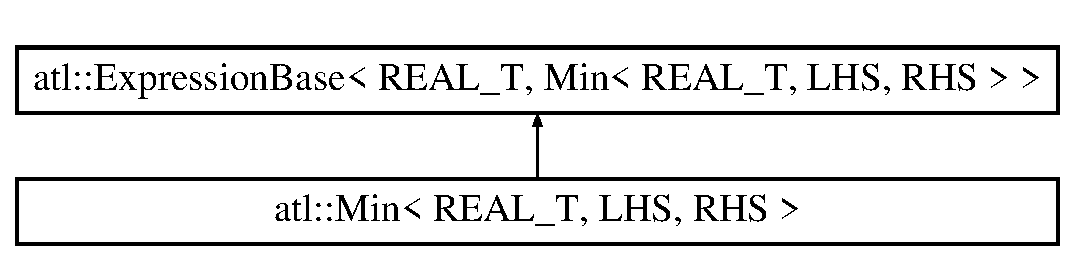
\includegraphics[height=2.000000cm]{structatl_1_1_min}
\end{center}
\end{figure}
\subsection*{Public Types}
\begin{DoxyCompactItemize}
\item 
\hypertarget{structatl_1_1_min_a37f513e8533cfbdb9b71214bc0368642}{typedef R\+E\+A\+L\+\_\+\+T {\bfseries B\+A\+S\+E\+\_\+\+T\+Y\+P\+E}}\label{structatl_1_1_min_a37f513e8533cfbdb9b71214bc0368642}

\end{DoxyCompactItemize}
\subsection*{Public Member Functions}
\begin{DoxyCompactItemize}
\item 
\hyperlink{structatl_1_1_min_ae1506e0989fba81a72845b2a87b948e1}{Min} (const \hyperlink{structatl_1_1_expression_base}{Expression\+Base}$<$ R\+E\+A\+L\+\_\+\+T, L\+H\+S $>$ \&lhs, const \hyperlink{structatl_1_1_expression_base}{Expression\+Base}$<$ R\+E\+A\+L\+\_\+\+T, R\+H\+S $>$ \&rhs)
\item 
\hyperlink{structatl_1_1_min_a906c567db23fd85ab69db559b63d86bc}{Min} (const R\+E\+A\+L\+\_\+\+T \&lhs, const \hyperlink{structatl_1_1_expression_base}{Expression\+Base}$<$ R\+E\+A\+L\+\_\+\+T, R\+H\+S $>$ \&rhs)
\item 
\hyperlink{structatl_1_1_min_ae2df8f5bb8b5cb4116d76f974d45c3b6}{Min} (const \hyperlink{structatl_1_1_expression_base}{Expression\+Base}$<$ R\+E\+A\+L\+\_\+\+T, L\+H\+S $>$ \&lhs, const R\+E\+A\+L\+\_\+\+T \&rhs)
\item 
const R\+E\+A\+L\+\_\+\+T \hyperlink{structatl_1_1_min_a28d3a51d455abad2ffcea957716193e4}{Get\+Value} () const 
\item 
const R\+E\+A\+L\+\_\+\+T \hyperlink{structatl_1_1_min_a90253b7bb0f9f6a6d98691297a459cba}{Get\+Value} (size\+\_\+t i, size\+\_\+t j=0) const 
\item 
void \hyperlink{structatl_1_1_min_a23e492722024fbbc49f9fe84f1028e90}{Push\+Ids} (typename \hyperlink{structatl_1_1_stack_entry}{atl\+::\+Stack\+Entry}$<$ R\+E\+A\+L\+\_\+\+T $>$\+::vi\+\_\+storage \&ids) const 
\item 
void \hyperlink{structatl_1_1_min_ace51856580ba941315279aef2ca70144}{Push\+Ids} (typename \hyperlink{structatl_1_1_stack_entry}{atl\+::\+Stack\+Entry}$<$ R\+E\+A\+L\+\_\+\+T $>$\+::vi\+\_\+storage \&ids, size\+\_\+t i, size\+\_\+t j=0) const 
\item 
R\+E\+A\+L\+\_\+\+T \hyperlink{structatl_1_1_min_aab9c8e3526585deef7fc2f91fa63fc92}{Evaluate\+Derivative} (uint32\+\_\+t x) const 
\item 
R\+E\+A\+L\+\_\+\+T \hyperlink{structatl_1_1_min_ada9c68d539700921a25f2a9753c6b5a5}{Evaluate\+Derivative} (uint32\+\_\+t x, uint32\+\_\+t y) const 
\item 
R\+E\+A\+L\+\_\+\+T \hyperlink{structatl_1_1_min_af0f047d817b4c3845302960cf982e7cd}{Evaluate\+Derivative} (uint32\+\_\+t x, uint32\+\_\+t y, uint32\+\_\+t z) const 
\item 
R\+E\+A\+L\+\_\+\+T \hyperlink{structatl_1_1_min_a2536d60b2ba7fccbfabfb954926579d3}{Evaluate\+Derivative} (uint32\+\_\+t x, size\+\_\+t i, size\+\_\+t j=0) const 
\item 
R\+E\+A\+L\+\_\+\+T \hyperlink{structatl_1_1_min_aab273fac4e70e3dfd25cdead2a51e49e}{Evaluate\+Derivative} (uint32\+\_\+t x, uint32\+\_\+t y, size\+\_\+t i, size\+\_\+t j=0) const 
\item 
R\+E\+A\+L\+\_\+\+T \hyperlink{structatl_1_1_min_ad33789ca233fe222fa23ecf9d4c47abd}{Evaluate\+Derivative} (uint32\+\_\+t x, uint32\+\_\+t y, uint32\+\_\+t z, size\+\_\+t i, size\+\_\+t j=0) const 
\item 
size\+\_\+t \hyperlink{structatl_1_1_min_a92ca2d47c3be558142f22073576d388b}{Get\+Columns} () const 
\item 
size\+\_\+t \hyperlink{structatl_1_1_min_a613235ceb818cbcf3f0d1d44566489eb}{Get\+Rows} () const 
\item 
bool \hyperlink{structatl_1_1_min_a79249d6f8fe8f0e72a76c5500017ba7b}{Is\+Scalar} () const 
\item 
const std\+::string \hyperlink{structatl_1_1_min_ae111fb7b6653e06443e8a0cc1f352a18}{To\+Expression\+Template\+String} () const 
\end{DoxyCompactItemize}
\subsection*{Public Attributes}
\begin{DoxyCompactItemize}
\item 
\hypertarget{structatl_1_1_min_a17a188bdd4acfa552709b9a6ef2f3054}{\hyperlink{structatl_1_1_real}{atl\+::\+Real}$<$ R\+E\+A\+L\+\_\+\+T $>$ {\bfseries real\+\_\+m}}\label{structatl_1_1_min_a17a188bdd4acfa552709b9a6ef2f3054}

\item 
\hypertarget{structatl_1_1_min_a6be647bd755e2552c340508397502ef0}{const L\+H\+S \& {\bfseries lhs\+\_\+m}}\label{structatl_1_1_min_a6be647bd755e2552c340508397502ef0}

\item 
\hypertarget{structatl_1_1_min_a1846550a7199fb5e71e01d7a8a2098ef}{const R\+H\+S \& {\bfseries rhs\+\_\+m}}\label{structatl_1_1_min_a1846550a7199fb5e71e01d7a8a2098ef}

\item 
\hypertarget{structatl_1_1_min_ad315ae7baf1e69e5657e16c5a89f2222}{R\+E\+A\+L\+\_\+\+T {\bfseries value\+\_\+m}}\label{structatl_1_1_min_ad315ae7baf1e69e5657e16c5a89f2222}

\item 
\hypertarget{structatl_1_1_min_a6ea602e9de7f7aff2080eccd16c8b2a2}{R\+E\+A\+L\+\_\+\+T {\bfseries C}}\label{structatl_1_1_min_a6ea602e9de7f7aff2080eccd16c8b2a2}

\end{DoxyCompactItemize}


\subsection{Constructor \& Destructor Documentation}
\hypertarget{structatl_1_1_min_ae1506e0989fba81a72845b2a87b948e1}{\index{atl\+::\+Min@{atl\+::\+Min}!Min@{Min}}
\index{Min@{Min}!atl\+::\+Min@{atl\+::\+Min}}
\subsubsection[{Min}]{\setlength{\rightskip}{0pt plus 5cm}template$<$class R\+E\+A\+L\+\_\+\+T , class L\+H\+S , class R\+H\+S $>$ {\bf atl\+::\+Min}$<$ R\+E\+A\+L\+\_\+\+T, L\+H\+S, R\+H\+S $>$\+::{\bf Min} (
\begin{DoxyParamCaption}
\item[{const {\bf Expression\+Base}$<$ R\+E\+A\+L\+\_\+\+T, L\+H\+S $>$ \&}]{lhs, }
\item[{const {\bf Expression\+Base}$<$ R\+E\+A\+L\+\_\+\+T, R\+H\+S $>$ \&}]{rhs}
\end{DoxyParamCaption}
)\hspace{0.3cm}{\ttfamily [inline]}}}\label{structatl_1_1_min_ae1506e0989fba81a72845b2a87b948e1}
Constructor for two variable types.


\begin{DoxyParams}{Parameters}
{\em lhs} & \\
\hline
{\em rhs} & \\
\hline
\end{DoxyParams}
\hypertarget{structatl_1_1_min_a906c567db23fd85ab69db559b63d86bc}{\index{atl\+::\+Min@{atl\+::\+Min}!Min@{Min}}
\index{Min@{Min}!atl\+::\+Min@{atl\+::\+Min}}
\subsubsection[{Min}]{\setlength{\rightskip}{0pt plus 5cm}template$<$class R\+E\+A\+L\+\_\+\+T , class L\+H\+S , class R\+H\+S $>$ {\bf atl\+::\+Min}$<$ R\+E\+A\+L\+\_\+\+T, L\+H\+S, R\+H\+S $>$\+::{\bf Min} (
\begin{DoxyParamCaption}
\item[{const R\+E\+A\+L\+\_\+\+T \&}]{lhs, }
\item[{const {\bf Expression\+Base}$<$ R\+E\+A\+L\+\_\+\+T, R\+H\+S $>$ \&}]{rhs}
\end{DoxyParamCaption}
)\hspace{0.3cm}{\ttfamily [inline]}}}\label{structatl_1_1_min_a906c567db23fd85ab69db559b63d86bc}
Constructor for real plus variable type. \hypertarget{structatl_1_1_min_ae2df8f5bb8b5cb4116d76f974d45c3b6}{\index{atl\+::\+Min@{atl\+::\+Min}!Min@{Min}}
\index{Min@{Min}!atl\+::\+Min@{atl\+::\+Min}}
\subsubsection[{Min}]{\setlength{\rightskip}{0pt plus 5cm}template$<$class R\+E\+A\+L\+\_\+\+T , class L\+H\+S , class R\+H\+S $>$ {\bf atl\+::\+Min}$<$ R\+E\+A\+L\+\_\+\+T, L\+H\+S, R\+H\+S $>$\+::{\bf Min} (
\begin{DoxyParamCaption}
\item[{const {\bf Expression\+Base}$<$ R\+E\+A\+L\+\_\+\+T, L\+H\+S $>$ \&}]{lhs, }
\item[{const R\+E\+A\+L\+\_\+\+T \&}]{rhs}
\end{DoxyParamCaption}
)\hspace{0.3cm}{\ttfamily [inline]}}}\label{structatl_1_1_min_ae2df8f5bb8b5cb4116d76f974d45c3b6}
Constructor for variable plus real type. 
\begin{DoxyParams}{Parameters}
{\em lhs} & \\
\hline
{\em rhs} & \\
\hline
\end{DoxyParams}


\subsection{Member Function Documentation}
\hypertarget{structatl_1_1_min_aab9c8e3526585deef7fc2f91fa63fc92}{\index{atl\+::\+Min@{atl\+::\+Min}!Evaluate\+Derivative@{Evaluate\+Derivative}}
\index{Evaluate\+Derivative@{Evaluate\+Derivative}!atl\+::\+Min@{atl\+::\+Min}}
\subsubsection[{Evaluate\+Derivative}]{\setlength{\rightskip}{0pt plus 5cm}template$<$class R\+E\+A\+L\+\_\+\+T , class L\+H\+S , class R\+H\+S $>$ R\+E\+A\+L\+\_\+\+T {\bf atl\+::\+Min}$<$ R\+E\+A\+L\+\_\+\+T, L\+H\+S, R\+H\+S $>$\+::Evaluate\+Derivative (
\begin{DoxyParamCaption}
\item[{uint32\+\_\+t}]{x}
\end{DoxyParamCaption}
) const\hspace{0.3cm}{\ttfamily [inline]}}}\label{structatl_1_1_min_aab9c8e3526585deef7fc2f91fa63fc92}
Evaluates the first-\/order derivative of this expression with respect to x.

$ {{d}\over{d\,x}}\,g\left(x\right)+{{d}\over{d\,x}}\,f\left(x\right) $


\begin{DoxyParams}{Parameters}
{\em x} & \\
\hline
\end{DoxyParams}
\begin{DoxyReturn}{Returns}

\end{DoxyReturn}
\hypertarget{structatl_1_1_min_ada9c68d539700921a25f2a9753c6b5a5}{\index{atl\+::\+Min@{atl\+::\+Min}!Evaluate\+Derivative@{Evaluate\+Derivative}}
\index{Evaluate\+Derivative@{Evaluate\+Derivative}!atl\+::\+Min@{atl\+::\+Min}}
\subsubsection[{Evaluate\+Derivative}]{\setlength{\rightskip}{0pt plus 5cm}template$<$class R\+E\+A\+L\+\_\+\+T , class L\+H\+S , class R\+H\+S $>$ R\+E\+A\+L\+\_\+\+T {\bf atl\+::\+Min}$<$ R\+E\+A\+L\+\_\+\+T, L\+H\+S, R\+H\+S $>$\+::Evaluate\+Derivative (
\begin{DoxyParamCaption}
\item[{uint32\+\_\+t}]{x, }
\item[{uint32\+\_\+t}]{y}
\end{DoxyParamCaption}
) const\hspace{0.3cm}{\ttfamily [inline]}}}\label{structatl_1_1_min_ada9c68d539700921a25f2a9753c6b5a5}
$ {{d^2}\over{d\,x\,d\,y}}\,g\left(x , y\right)+{{d^2}\over{d\,x\,d\, y}}\,f\left(x , y\right) $ 
\begin{DoxyParams}{Parameters}
{\em x} & \\
\hline
{\em y} & \\
\hline
\end{DoxyParams}
\begin{DoxyReturn}{Returns}

\end{DoxyReturn}
\hypertarget{structatl_1_1_min_af0f047d817b4c3845302960cf982e7cd}{\index{atl\+::\+Min@{atl\+::\+Min}!Evaluate\+Derivative@{Evaluate\+Derivative}}
\index{Evaluate\+Derivative@{Evaluate\+Derivative}!atl\+::\+Min@{atl\+::\+Min}}
\subsubsection[{Evaluate\+Derivative}]{\setlength{\rightskip}{0pt plus 5cm}template$<$class R\+E\+A\+L\+\_\+\+T , class L\+H\+S , class R\+H\+S $>$ R\+E\+A\+L\+\_\+\+T {\bf atl\+::\+Min}$<$ R\+E\+A\+L\+\_\+\+T, L\+H\+S, R\+H\+S $>$\+::Evaluate\+Derivative (
\begin{DoxyParamCaption}
\item[{uint32\+\_\+t}]{x, }
\item[{uint32\+\_\+t}]{y, }
\item[{uint32\+\_\+t}]{z}
\end{DoxyParamCaption}
) const\hspace{0.3cm}{\ttfamily [inline]}}}\label{structatl_1_1_min_af0f047d817b4c3845302960cf982e7cd}
$ {{d^3}\over{d\,x\,d\,y\,d\,z}}\,g\left(x , y , z\right)+{{d^3 }\over{d\,x\,d\,y\,d\,z}}\,f\left(x , y , z\right) $ 
\begin{DoxyParams}{Parameters}
{\em x} & \\
\hline
{\em y} & \\
\hline
{\em z} & \\
\hline
\end{DoxyParams}
\begin{DoxyReturn}{Returns}

\end{DoxyReturn}
\hypertarget{structatl_1_1_min_a2536d60b2ba7fccbfabfb954926579d3}{\index{atl\+::\+Min@{atl\+::\+Min}!Evaluate\+Derivative@{Evaluate\+Derivative}}
\index{Evaluate\+Derivative@{Evaluate\+Derivative}!atl\+::\+Min@{atl\+::\+Min}}
\subsubsection[{Evaluate\+Derivative}]{\setlength{\rightskip}{0pt plus 5cm}template$<$class R\+E\+A\+L\+\_\+\+T , class L\+H\+S , class R\+H\+S $>$ R\+E\+A\+L\+\_\+\+T {\bf atl\+::\+Min}$<$ R\+E\+A\+L\+\_\+\+T, L\+H\+S, R\+H\+S $>$\+::Evaluate\+Derivative (
\begin{DoxyParamCaption}
\item[{uint32\+\_\+t}]{x, }
\item[{size\+\_\+t}]{i, }
\item[{size\+\_\+t}]{j = {\ttfamily 0}}
\end{DoxyParamCaption}
) const\hspace{0.3cm}{\ttfamily [inline]}}}\label{structatl_1_1_min_a2536d60b2ba7fccbfabfb954926579d3}
Evaluates the first-\/order derivative of this expression with respect to x at index \{i,j\}.


\begin{DoxyParams}{Parameters}
{\em a} & \\
\hline
{\em i} & \\
\hline
{\em j} & \\
\hline
\end{DoxyParams}
\begin{DoxyReturn}{Returns}

\end{DoxyReturn}
\hypertarget{structatl_1_1_min_aab273fac4e70e3dfd25cdead2a51e49e}{\index{atl\+::\+Min@{atl\+::\+Min}!Evaluate\+Derivative@{Evaluate\+Derivative}}
\index{Evaluate\+Derivative@{Evaluate\+Derivative}!atl\+::\+Min@{atl\+::\+Min}}
\subsubsection[{Evaluate\+Derivative}]{\setlength{\rightskip}{0pt plus 5cm}template$<$class R\+E\+A\+L\+\_\+\+T , class L\+H\+S , class R\+H\+S $>$ R\+E\+A\+L\+\_\+\+T {\bf atl\+::\+Min}$<$ R\+E\+A\+L\+\_\+\+T, L\+H\+S, R\+H\+S $>$\+::Evaluate\+Derivative (
\begin{DoxyParamCaption}
\item[{uint32\+\_\+t}]{x, }
\item[{uint32\+\_\+t}]{y, }
\item[{size\+\_\+t}]{i, }
\item[{size\+\_\+t}]{j = {\ttfamily 0}}
\end{DoxyParamCaption}
) const\hspace{0.3cm}{\ttfamily [inline]}}}\label{structatl_1_1_min_aab273fac4e70e3dfd25cdead2a51e49e}

\begin{DoxyParams}{Parameters}
{\em x} & \\
\hline
{\em y} & \\
\hline
{\em i} & \\
\hline
{\em j} & \\
\hline
\end{DoxyParams}
\begin{DoxyReturn}{Returns}

\end{DoxyReturn}
\hypertarget{structatl_1_1_min_ad33789ca233fe222fa23ecf9d4c47abd}{\index{atl\+::\+Min@{atl\+::\+Min}!Evaluate\+Derivative@{Evaluate\+Derivative}}
\index{Evaluate\+Derivative@{Evaluate\+Derivative}!atl\+::\+Min@{atl\+::\+Min}}
\subsubsection[{Evaluate\+Derivative}]{\setlength{\rightskip}{0pt plus 5cm}template$<$class R\+E\+A\+L\+\_\+\+T , class L\+H\+S , class R\+H\+S $>$ R\+E\+A\+L\+\_\+\+T {\bf atl\+::\+Min}$<$ R\+E\+A\+L\+\_\+\+T, L\+H\+S, R\+H\+S $>$\+::Evaluate\+Derivative (
\begin{DoxyParamCaption}
\item[{uint32\+\_\+t}]{x, }
\item[{uint32\+\_\+t}]{y, }
\item[{uint32\+\_\+t}]{z, }
\item[{size\+\_\+t}]{i, }
\item[{size\+\_\+t}]{j = {\ttfamily 0}}
\end{DoxyParamCaption}
) const\hspace{0.3cm}{\ttfamily [inline]}}}\label{structatl_1_1_min_ad33789ca233fe222fa23ecf9d4c47abd}

\begin{DoxyParams}{Parameters}
{\em x} & \\
\hline
{\em y} & \\
\hline
{\em z} & \\
\hline
{\em i} & \\
\hline
{\em j} & \\
\hline
\end{DoxyParams}
\begin{DoxyReturn}{Returns}

\end{DoxyReturn}
\hypertarget{structatl_1_1_min_a92ca2d47c3be558142f22073576d388b}{\index{atl\+::\+Min@{atl\+::\+Min}!Get\+Columns@{Get\+Columns}}
\index{Get\+Columns@{Get\+Columns}!atl\+::\+Min@{atl\+::\+Min}}
\subsubsection[{Get\+Columns}]{\setlength{\rightskip}{0pt plus 5cm}template$<$class R\+E\+A\+L\+\_\+\+T , class L\+H\+S , class R\+H\+S $>$ size\+\_\+t {\bf atl\+::\+Min}$<$ R\+E\+A\+L\+\_\+\+T, L\+H\+S, R\+H\+S $>$\+::Get\+Columns (
\begin{DoxyParamCaption}
{}
\end{DoxyParamCaption}
) const\hspace{0.3cm}{\ttfamily [inline]}}}\label{structatl_1_1_min_a92ca2d47c3be558142f22073576d388b}
Return the number of columns.

\begin{DoxyReturn}{Returns}

\end{DoxyReturn}
\hypertarget{structatl_1_1_min_a613235ceb818cbcf3f0d1d44566489eb}{\index{atl\+::\+Min@{atl\+::\+Min}!Get\+Rows@{Get\+Rows}}
\index{Get\+Rows@{Get\+Rows}!atl\+::\+Min@{atl\+::\+Min}}
\subsubsection[{Get\+Rows}]{\setlength{\rightskip}{0pt plus 5cm}template$<$class R\+E\+A\+L\+\_\+\+T , class L\+H\+S , class R\+H\+S $>$ size\+\_\+t {\bf atl\+::\+Min}$<$ R\+E\+A\+L\+\_\+\+T, L\+H\+S, R\+H\+S $>$\+::Get\+Rows (
\begin{DoxyParamCaption}
{}
\end{DoxyParamCaption}
) const\hspace{0.3cm}{\ttfamily [inline]}}}\label{structatl_1_1_min_a613235ceb818cbcf3f0d1d44566489eb}
Return the number of rows.

\begin{DoxyReturn}{Returns}

\end{DoxyReturn}
\hypertarget{structatl_1_1_min_a28d3a51d455abad2ffcea957716193e4}{\index{atl\+::\+Min@{atl\+::\+Min}!Get\+Value@{Get\+Value}}
\index{Get\+Value@{Get\+Value}!atl\+::\+Min@{atl\+::\+Min}}
\subsubsection[{Get\+Value}]{\setlength{\rightskip}{0pt plus 5cm}template$<$class R\+E\+A\+L\+\_\+\+T , class L\+H\+S , class R\+H\+S $>$ const R\+E\+A\+L\+\_\+\+T {\bf atl\+::\+Min}$<$ R\+E\+A\+L\+\_\+\+T, L\+H\+S, R\+H\+S $>$\+::Get\+Value (
\begin{DoxyParamCaption}
{}
\end{DoxyParamCaption}
) const\hspace{0.3cm}{\ttfamily [inline]}}}\label{structatl_1_1_min_a28d3a51d455abad2ffcea957716193e4}
Compute the min of the lhs and rhs expressions.

\begin{DoxyReturn}{Returns}

\end{DoxyReturn}
\hypertarget{structatl_1_1_min_a90253b7bb0f9f6a6d98691297a459cba}{\index{atl\+::\+Min@{atl\+::\+Min}!Get\+Value@{Get\+Value}}
\index{Get\+Value@{Get\+Value}!atl\+::\+Min@{atl\+::\+Min}}
\subsubsection[{Get\+Value}]{\setlength{\rightskip}{0pt plus 5cm}template$<$class R\+E\+A\+L\+\_\+\+T , class L\+H\+S , class R\+H\+S $>$ const R\+E\+A\+L\+\_\+\+T {\bf atl\+::\+Min}$<$ R\+E\+A\+L\+\_\+\+T, L\+H\+S, R\+H\+S $>$\+::Get\+Value (
\begin{DoxyParamCaption}
\item[{size\+\_\+t}]{i, }
\item[{size\+\_\+t}]{j = {\ttfamily 0}}
\end{DoxyParamCaption}
) const\hspace{0.3cm}{\ttfamily [inline]}}}\label{structatl_1_1_min_a90253b7bb0f9f6a6d98691297a459cba}
Compute the min of the lhs and rhs expressions at index \{i,j\}.

\begin{DoxyReturn}{Returns}

\end{DoxyReturn}
\hypertarget{structatl_1_1_min_a79249d6f8fe8f0e72a76c5500017ba7b}{\index{atl\+::\+Min@{atl\+::\+Min}!Is\+Scalar@{Is\+Scalar}}
\index{Is\+Scalar@{Is\+Scalar}!atl\+::\+Min@{atl\+::\+Min}}
\subsubsection[{Is\+Scalar}]{\setlength{\rightskip}{0pt plus 5cm}template$<$class R\+E\+A\+L\+\_\+\+T , class L\+H\+S , class R\+H\+S $>$ bool {\bf atl\+::\+Min}$<$ R\+E\+A\+L\+\_\+\+T, L\+H\+S, R\+H\+S $>$\+::Is\+Scalar (
\begin{DoxyParamCaption}
{}
\end{DoxyParamCaption}
) const\hspace{0.3cm}{\ttfamily [inline]}}}\label{structatl_1_1_min_a79249d6f8fe8f0e72a76c5500017ba7b}
True if the expression is a scalar. \begin{DoxyReturn}{Returns}

\end{DoxyReturn}
\hypertarget{structatl_1_1_min_a23e492722024fbbc49f9fe84f1028e90}{\index{atl\+::\+Min@{atl\+::\+Min}!Push\+Ids@{Push\+Ids}}
\index{Push\+Ids@{Push\+Ids}!atl\+::\+Min@{atl\+::\+Min}}
\subsubsection[{Push\+Ids}]{\setlength{\rightskip}{0pt plus 5cm}template$<$class R\+E\+A\+L\+\_\+\+T , class L\+H\+S , class R\+H\+S $>$ void {\bf atl\+::\+Min}$<$ R\+E\+A\+L\+\_\+\+T, L\+H\+S, R\+H\+S $>$\+::Push\+Ids (
\begin{DoxyParamCaption}
\item[{typename {\bf atl\+::\+Stack\+Entry}$<$ R\+E\+A\+L\+\_\+\+T $>$\+::vi\+\_\+storage \&}]{ids}
\end{DoxyParamCaption}
) const\hspace{0.3cm}{\ttfamily [inline]}}}\label{structatl_1_1_min_a23e492722024fbbc49f9fe84f1028e90}
Push variable info into a set.


\begin{DoxyParams}{Parameters}
{\em ids} & \\
\hline
{\em i} & \\
\hline
{\em j} & \\
\hline
\end{DoxyParams}
\hypertarget{structatl_1_1_min_ace51856580ba941315279aef2ca70144}{\index{atl\+::\+Min@{atl\+::\+Min}!Push\+Ids@{Push\+Ids}}
\index{Push\+Ids@{Push\+Ids}!atl\+::\+Min@{atl\+::\+Min}}
\subsubsection[{Push\+Ids}]{\setlength{\rightskip}{0pt plus 5cm}template$<$class R\+E\+A\+L\+\_\+\+T , class L\+H\+S , class R\+H\+S $>$ void {\bf atl\+::\+Min}$<$ R\+E\+A\+L\+\_\+\+T, L\+H\+S, R\+H\+S $>$\+::Push\+Ids (
\begin{DoxyParamCaption}
\item[{typename {\bf atl\+::\+Stack\+Entry}$<$ R\+E\+A\+L\+\_\+\+T $>$\+::vi\+\_\+storage \&}]{ids, }
\item[{size\+\_\+t}]{i, }
\item[{size\+\_\+t}]{j = {\ttfamily 0}}
\end{DoxyParamCaption}
) const\hspace{0.3cm}{\ttfamily [inline]}}}\label{structatl_1_1_min_ace51856580ba941315279aef2ca70144}
Push variable info into a set at index \{i,j\}.


\begin{DoxyParams}{Parameters}
{\em ids} & \\
\hline
{\em i} & \\
\hline
{\em j} & \\
\hline
\end{DoxyParams}
\hypertarget{structatl_1_1_min_ae111fb7b6653e06443e8a0cc1f352a18}{\index{atl\+::\+Min@{atl\+::\+Min}!To\+Expression\+Template\+String@{To\+Expression\+Template\+String}}
\index{To\+Expression\+Template\+String@{To\+Expression\+Template\+String}!atl\+::\+Min@{atl\+::\+Min}}
\subsubsection[{To\+Expression\+Template\+String}]{\setlength{\rightskip}{0pt plus 5cm}template$<$class R\+E\+A\+L\+\_\+\+T , class L\+H\+S , class R\+H\+S $>$ const std\+::string {\bf atl\+::\+Min}$<$ R\+E\+A\+L\+\_\+\+T, L\+H\+S, R\+H\+S $>$\+::To\+Expression\+Template\+String (
\begin{DoxyParamCaption}
{}
\end{DoxyParamCaption}
) const\hspace{0.3cm}{\ttfamily [inline]}}}\label{structatl_1_1_min_ae111fb7b6653e06443e8a0cc1f352a18}
Create a string representation of this expression template. \begin{DoxyReturn}{Returns}

\end{DoxyReturn}


The documentation for this struct was generated from the following file\+:\begin{DoxyCompactItemize}
\item 
Min\+Max.\+hpp\end{DoxyCompactItemize}

\hypertarget{structatl_1_1_multiply}{\section{atl\+:\+:Multiply$<$ R\+E\+A\+L\+\_\+\+T, L\+H\+S, R\+H\+S $>$ Struct Template Reference}
\label{structatl_1_1_multiply}\index{atl\+::\+Multiply$<$ R\+E\+A\+L\+\_\+\+T, L\+H\+S, R\+H\+S $>$@{atl\+::\+Multiply$<$ R\+E\+A\+L\+\_\+\+T, L\+H\+S, R\+H\+S $>$}}
}


{\ttfamily \#include $<$Multiply.\+hpp$>$}

Inheritance diagram for atl\+:\+:Multiply$<$ R\+E\+A\+L\+\_\+\+T, L\+H\+S, R\+H\+S $>$\+:\begin{figure}[H]
\begin{center}
\leavevmode
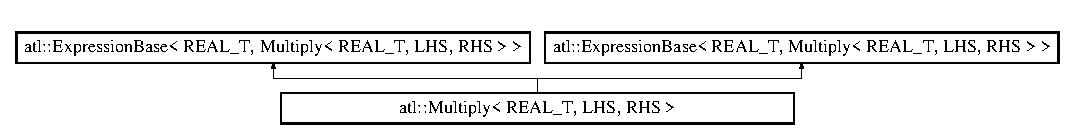
\includegraphics[height=1.439589cm]{structatl_1_1_multiply}
\end{center}
\end{figure}
\subsection*{Public Member Functions}
\begin{DoxyCompactItemize}
\item 
\hypertarget{structatl_1_1_multiply_a71353c701201490c6ee810658d4fb953}{{\bfseries Multiply} (const \hyperlink{structatl_1_1_expression_base}{Expression\+Base}$<$ R\+E\+A\+L\+\_\+\+T, L\+H\+S $>$ \&lhs, const \hyperlink{structatl_1_1_expression_base}{Expression\+Base}$<$ R\+E\+A\+L\+\_\+\+T, R\+H\+S $>$ \&rhs)}\label{structatl_1_1_multiply_a71353c701201490c6ee810658d4fb953}

\item 
\hypertarget{structatl_1_1_multiply_ac614c1ef3b3c6bf4e46dadf8d9b0538b}{{\bfseries Multiply} (const R\+E\+A\+L\+\_\+\+T \&lhs, const \hyperlink{structatl_1_1_expression_base}{Expression\+Base}$<$ R\+E\+A\+L\+\_\+\+T, R\+H\+S $>$ \&rhs)}\label{structatl_1_1_multiply_ac614c1ef3b3c6bf4e46dadf8d9b0538b}

\item 
\hypertarget{structatl_1_1_multiply_a7b863518694411a59bc103be12d73cbb}{{\bfseries Multiply} (const \hyperlink{structatl_1_1_expression_base}{Expression\+Base}$<$ R\+E\+A\+L\+\_\+\+T, L\+H\+S $>$ \&lhs, const R\+E\+A\+L\+\_\+\+T \&rhs)}\label{structatl_1_1_multiply_a7b863518694411a59bc103be12d73cbb}

\item 
\hypertarget{structatl_1_1_multiply_a2ea701e5cef0632f5c27cb626e1f165f}{const R\+E\+A\+L\+\_\+\+T {\bfseries Get\+Value} () const }\label{structatl_1_1_multiply_a2ea701e5cef0632f5c27cb626e1f165f}

\item 
\hypertarget{structatl_1_1_multiply_a5a28954726bf2016e94564e587013c7f}{const R\+E\+A\+L\+\_\+\+T {\bfseries Get\+Value} (size\+\_\+t i, size\+\_\+t j=0) const }\label{structatl_1_1_multiply_a5a28954726bf2016e94564e587013c7f}

\item 
\hypertarget{structatl_1_1_multiply_ad2a09b1cf0d1dbe48b3a532cba272eeb}{void {\bfseries Push\+Ids} (typename \hyperlink{structatl_1_1_stack_entry}{atl\+::\+Stack\+Entry}$<$ R\+E\+A\+L\+\_\+\+T $>$\+::vi\+\_\+storage \&ids) const }\label{structatl_1_1_multiply_ad2a09b1cf0d1dbe48b3a532cba272eeb}

\item 
\hypertarget{structatl_1_1_multiply_a90777da934335b5320b4975fbeb332fc}{void {\bfseries Push\+Ids} (typename \hyperlink{structatl_1_1_stack_entry}{atl\+::\+Stack\+Entry}$<$ R\+E\+A\+L\+\_\+\+T $>$\+::vi\+\_\+storage \&ids, size\+\_\+t i, size\+\_\+t j=0) const }\label{structatl_1_1_multiply_a90777da934335b5320b4975fbeb332fc}

\item 
\hypertarget{structatl_1_1_multiply_adac83a483dd8268e7d0d0e38d1235bad}{const R\+E\+A\+L\+\_\+\+T {\bfseries Evaluate\+Derivative} (uint32\+\_\+t id) const }\label{structatl_1_1_multiply_adac83a483dd8268e7d0d0e38d1235bad}

\item 
\hypertarget{structatl_1_1_multiply_a2bf46a9ea8e1c71ffe8f9c79f4f98767}{R\+E\+A\+L\+\_\+\+T {\bfseries Evaluate\+Derivative} (uint32\+\_\+t a, uint32\+\_\+t b) const }\label{structatl_1_1_multiply_a2bf46a9ea8e1c71ffe8f9c79f4f98767}

\item 
\hypertarget{structatl_1_1_multiply_a9dbc68b47f2687a2a3e510b1e30b25e1}{R\+E\+A\+L\+\_\+\+T {\bfseries Evaluate\+Derivative} (uint32\+\_\+t x, uint32\+\_\+t y, uint32\+\_\+t z) const }\label{structatl_1_1_multiply_a9dbc68b47f2687a2a3e510b1e30b25e1}

\item 
\hypertarget{structatl_1_1_multiply_a0756c346a650747f8ffc4a63b8019586}{R\+E\+A\+L\+\_\+\+T {\bfseries Evaluate\+Derivative} (uint32\+\_\+t a, size\+\_\+t i, size\+\_\+t j=0) const }\label{structatl_1_1_multiply_a0756c346a650747f8ffc4a63b8019586}

\item 
\hypertarget{structatl_1_1_multiply_a869b949cd670c488f1999afe5bb9b187}{R\+E\+A\+L\+\_\+\+T {\bfseries Evaluate\+Derivative} (uint32\+\_\+t a, uint32\+\_\+t b, size\+\_\+t i, size\+\_\+t j=0) const }\label{structatl_1_1_multiply_a869b949cd670c488f1999afe5bb9b187}

\item 
\hypertarget{structatl_1_1_multiply_ad96c2a68a427fb698c6a415a37fbec2b}{R\+E\+A\+L\+\_\+\+T {\bfseries Evaluate\+Derivative} (uint32\+\_\+t x, uint32\+\_\+t y, uint32\+\_\+t z, size\+\_\+t i, size\+\_\+t j=0) const }\label{structatl_1_1_multiply_ad96c2a68a427fb698c6a415a37fbec2b}

\item 
\hypertarget{structatl_1_1_multiply_ad0be7a6012b64cd7d0991580e92d63cb}{size\+\_\+t {\bfseries Get\+Columns} () const }\label{structatl_1_1_multiply_ad0be7a6012b64cd7d0991580e92d63cb}

\item 
\hypertarget{structatl_1_1_multiply_a38339891d6ef8ee51ad41376f3dcc222}{size\+\_\+t {\bfseries Get\+Rows} () const }\label{structatl_1_1_multiply_a38339891d6ef8ee51ad41376f3dcc222}

\item 
\hypertarget{structatl_1_1_multiply_ab7b229dc85f278cd1e734d818b2cfe82}{bool {\bfseries Is\+Scalar} () const }\label{structatl_1_1_multiply_ab7b229dc85f278cd1e734d818b2cfe82}

\item 
\hyperlink{structatl_1_1_multiply_a71353c701201490c6ee810658d4fb953}{Multiply} (const \hyperlink{structatl_1_1_expression_base}{Expression\+Base}$<$ R\+E\+A\+L\+\_\+\+T, L\+H\+S $>$ \&lhs, const \hyperlink{structatl_1_1_expression_base}{Expression\+Base}$<$ R\+E\+A\+L\+\_\+\+T, R\+H\+S $>$ \&rhs)
\item 
\hyperlink{structatl_1_1_multiply_ac614c1ef3b3c6bf4e46dadf8d9b0538b}{Multiply} (const R\+E\+A\+L\+\_\+\+T \&lhs, const \hyperlink{structatl_1_1_expression_base}{Expression\+Base}$<$ R\+E\+A\+L\+\_\+\+T, R\+H\+S $>$ \&rhs)
\item 
\hyperlink{structatl_1_1_multiply_a7b863518694411a59bc103be12d73cbb}{Multiply} (const \hyperlink{structatl_1_1_expression_base}{Expression\+Base}$<$ R\+E\+A\+L\+\_\+\+T, L\+H\+S $>$ \&lhs, const R\+E\+A\+L\+\_\+\+T \&rhs)
\item 
const R\+E\+A\+L\+\_\+\+T \hyperlink{structatl_1_1_multiply_a2ea701e5cef0632f5c27cb626e1f165f}{Get\+Value} () const 
\item 
const R\+E\+A\+L\+\_\+\+T \hyperlink{structatl_1_1_multiply_a5a28954726bf2016e94564e587013c7f}{Get\+Value} (size\+\_\+t i, size\+\_\+t j=0) const 
\item 
bool \hyperlink{structatl_1_1_multiply_a788bf22cc55af594eb50cc56f901ef90}{Is\+Nonlinear} () const 
\item 
void \hyperlink{structatl_1_1_multiply_ad2a09b1cf0d1dbe48b3a532cba272eeb}{Push\+Ids} (typename \hyperlink{structatl_1_1_stack_entry}{atl\+::\+Stack\+Entry}$<$ R\+E\+A\+L\+\_\+\+T $>$\+::vi\+\_\+storage \&ids) const 
\item 
void \hyperlink{structatl_1_1_multiply_a90777da934335b5320b4975fbeb332fc}{Push\+Ids} (typename \hyperlink{structatl_1_1_stack_entry}{atl\+::\+Stack\+Entry}$<$ R\+E\+A\+L\+\_\+\+T $>$\+::vi\+\_\+storage \&ids, size\+\_\+t i, size\+\_\+t j=0) const 
\item 
const R\+E\+A\+L\+\_\+\+T \hyperlink{structatl_1_1_multiply_ac9c7ec127366992b536d53162b783c0f}{Evaluate\+Derivative} (uint32\+\_\+t x) const 
\item 
R\+E\+A\+L\+\_\+\+T \hyperlink{structatl_1_1_multiply_a7d4dd40f6f10423bed06cd94dc32c230}{Evaluate\+Derivative} (uint32\+\_\+t x, uint32\+\_\+t y) const 
\item 
R\+E\+A\+L\+\_\+\+T \hyperlink{structatl_1_1_multiply_a9dbc68b47f2687a2a3e510b1e30b25e1}{Evaluate\+Derivative} (uint32\+\_\+t x, uint32\+\_\+t y, uint32\+\_\+t z) const 
\item 
R\+E\+A\+L\+\_\+\+T \hyperlink{structatl_1_1_multiply_aaf3d6bff82038810945ee401d02b840d}{Evaluate\+Derivative} (uint32\+\_\+t x, size\+\_\+t i, size\+\_\+t j=0) const 
\item 
R\+E\+A\+L\+\_\+\+T \hyperlink{structatl_1_1_multiply_ad4723c06544039782a1787184f442e08}{Evaluate\+Derivative} (uint32\+\_\+t x, uint32\+\_\+t y, size\+\_\+t i, size\+\_\+t j=0) const 
\item 
R\+E\+A\+L\+\_\+\+T \hyperlink{structatl_1_1_multiply_ad96c2a68a427fb698c6a415a37fbec2b}{Evaluate\+Derivative} (uint32\+\_\+t x, uint32\+\_\+t y, uint32\+\_\+t z, size\+\_\+t i, size\+\_\+t j=0) const 
\item 
size\+\_\+t \hyperlink{structatl_1_1_multiply_ad0be7a6012b64cd7d0991580e92d63cb}{Get\+Columns} () const 
\item 
size\+\_\+t \hyperlink{structatl_1_1_multiply_a38339891d6ef8ee51ad41376f3dcc222}{Get\+Rows} () const 
\item 
bool \hyperlink{structatl_1_1_multiply_ab7b229dc85f278cd1e734d818b2cfe82}{Is\+Scalar} () const 
\item 
const std\+::string \hyperlink{structatl_1_1_multiply_a7af1cf8911863ad6b83ccba63fa7df52}{To\+Expression\+Template\+String} () const 
\end{DoxyCompactItemize}
\subsection*{Public Attributes}
\begin{DoxyCompactItemize}
\item 
\hypertarget{structatl_1_1_multiply_a545f4e305d26b37ea0c305c7a7477176}{bool {\bfseries mm\+\_\+multiply} = false}\label{structatl_1_1_multiply_a545f4e305d26b37ea0c305c7a7477176}

\item 
\hypertarget{structatl_1_1_multiply_a2cd7b240c36d5fd720efaadaeaf395ea}{\hyperlink{structatl_1_1_real}{atl\+::\+Real}$<$ R\+E\+A\+L\+\_\+\+T $>$ {\bfseries real\+\_\+m}}\label{structatl_1_1_multiply_a2cd7b240c36d5fd720efaadaeaf395ea}

\item 
\hypertarget{structatl_1_1_multiply_a7f974ac48df77cb13ae0a32421c74224}{const L\+H\+S \& {\bfseries lhs\+\_\+m}}\label{structatl_1_1_multiply_a7f974ac48df77cb13ae0a32421c74224}

\item 
\hypertarget{structatl_1_1_multiply_a42844c51219f21e9f376e03f60bc42b1}{const R\+H\+S \& {\bfseries rhs\+\_\+m}}\label{structatl_1_1_multiply_a42844c51219f21e9f376e03f60bc42b1}

\item 
\hypertarget{structatl_1_1_multiply_a1a4a982e56c168c37ae3e79975f9edec}{R\+E\+A\+L\+\_\+\+T {\bfseries value\+\_\+m}}\label{structatl_1_1_multiply_a1a4a982e56c168c37ae3e79975f9edec}

\end{DoxyCompactItemize}


\subsection{Detailed Description}
\subsubsection*{template$<$class R\+E\+A\+L\+\_\+\+T, class L\+H\+S, class R\+H\+S$>$struct atl\+::\+Multiply$<$ R\+E\+A\+L\+\_\+\+T, L\+H\+S, R\+H\+S $>$}

Expression template to handle multiplication.

$ f(x) * g(x) $

or

$ f_{i,j}(x) * g_{i,j}(x) $ 

\subsection{Constructor \& Destructor Documentation}
\hypertarget{structatl_1_1_multiply_a71353c701201490c6ee810658d4fb953}{\index{atl\+::\+Multiply@{atl\+::\+Multiply}!Multiply@{Multiply}}
\index{Multiply@{Multiply}!atl\+::\+Multiply@{atl\+::\+Multiply}}
\subsubsection[{Multiply}]{\setlength{\rightskip}{0pt plus 5cm}template$<$class R\+E\+A\+L\+\_\+\+T, class L\+H\+S , class R\+H\+S $>$ {\bf atl\+::\+Multiply}$<$ R\+E\+A\+L\+\_\+\+T, L\+H\+S, R\+H\+S $>$\+::{\bf Multiply} (
\begin{DoxyParamCaption}
\item[{const {\bf Expression\+Base}$<$ R\+E\+A\+L\+\_\+\+T, L\+H\+S $>$ \&}]{lhs, }
\item[{const {\bf Expression\+Base}$<$ R\+E\+A\+L\+\_\+\+T, R\+H\+S $>$ \&}]{rhs}
\end{DoxyParamCaption}
)\hspace{0.3cm}{\ttfamily [inline]}}}\label{structatl_1_1_multiply_a71353c701201490c6ee810658d4fb953}
Constructor for \hyperlink{structatl_1_1_variable}{Variable} types.


\begin{DoxyParams}{Parameters}
{\em lhs} & \\
\hline
{\em rhs} & \\
\hline
\end{DoxyParams}
\hypertarget{structatl_1_1_multiply_ac614c1ef3b3c6bf4e46dadf8d9b0538b}{\index{atl\+::\+Multiply@{atl\+::\+Multiply}!Multiply@{Multiply}}
\index{Multiply@{Multiply}!atl\+::\+Multiply@{atl\+::\+Multiply}}
\subsubsection[{Multiply}]{\setlength{\rightskip}{0pt plus 5cm}template$<$class R\+E\+A\+L\+\_\+\+T, class L\+H\+S , class R\+H\+S $>$ {\bf atl\+::\+Multiply}$<$ R\+E\+A\+L\+\_\+\+T, L\+H\+S, R\+H\+S $>$\+::{\bf Multiply} (
\begin{DoxyParamCaption}
\item[{const R\+E\+A\+L\+\_\+\+T \&}]{lhs, }
\item[{const {\bf Expression\+Base}$<$ R\+E\+A\+L\+\_\+\+T, R\+H\+S $>$ \&}]{rhs}
\end{DoxyParamCaption}
)\hspace{0.3cm}{\ttfamily [inline]}}}\label{structatl_1_1_multiply_ac614c1ef3b3c6bf4e46dadf8d9b0538b}
Constructor for a real and \hyperlink{structatl_1_1_variable}{Variable} type.


\begin{DoxyParams}{Parameters}
{\em lhs} & \\
\hline
{\em rhs} & \\
\hline
\end{DoxyParams}
\hypertarget{structatl_1_1_multiply_a7b863518694411a59bc103be12d73cbb}{\index{atl\+::\+Multiply@{atl\+::\+Multiply}!Multiply@{Multiply}}
\index{Multiply@{Multiply}!atl\+::\+Multiply@{atl\+::\+Multiply}}
\subsubsection[{Multiply}]{\setlength{\rightskip}{0pt plus 5cm}template$<$class R\+E\+A\+L\+\_\+\+T, class L\+H\+S , class R\+H\+S $>$ {\bf atl\+::\+Multiply}$<$ R\+E\+A\+L\+\_\+\+T, L\+H\+S, R\+H\+S $>$\+::{\bf Multiply} (
\begin{DoxyParamCaption}
\item[{const {\bf Expression\+Base}$<$ R\+E\+A\+L\+\_\+\+T, L\+H\+S $>$ \&}]{lhs, }
\item[{const R\+E\+A\+L\+\_\+\+T \&}]{rhs}
\end{DoxyParamCaption}
)\hspace{0.3cm}{\ttfamily [inline]}}}\label{structatl_1_1_multiply_a7b863518694411a59bc103be12d73cbb}
Constructor for \hyperlink{structatl_1_1_variable}{Variable} and real type.


\begin{DoxyParams}{Parameters}
{\em lhs} & \\
\hline
{\em rhs} & \\
\hline
\end{DoxyParams}


\subsection{Member Function Documentation}
\hypertarget{structatl_1_1_multiply_ac9c7ec127366992b536d53162b783c0f}{\index{atl\+::\+Multiply@{atl\+::\+Multiply}!Evaluate\+Derivative@{Evaluate\+Derivative}}
\index{Evaluate\+Derivative@{Evaluate\+Derivative}!atl\+::\+Multiply@{atl\+::\+Multiply}}
\subsubsection[{Evaluate\+Derivative}]{\setlength{\rightskip}{0pt plus 5cm}template$<$class R\+E\+A\+L\+\_\+\+T, class L\+H\+S , class R\+H\+S $>$ const R\+E\+A\+L\+\_\+\+T {\bf atl\+::\+Multiply}$<$ R\+E\+A\+L\+\_\+\+T, L\+H\+S, R\+H\+S $>$\+::Evaluate\+Derivative (
\begin{DoxyParamCaption}
\item[{uint32\+\_\+t}]{x}
\end{DoxyParamCaption}
) const\hspace{0.3cm}{\ttfamily [inline]}}}\label{structatl_1_1_multiply_ac9c7ec127366992b536d53162b783c0f}
Evaluates the derivative of this expression with respect to x.

$f\left(x\right)\,\left({{d}\over{d\,x}}\,g\left(x\right)\right)+g\left(x\right)\,\left({{d}\over{d\,x}}\,f\left(x\right)\right)$


\begin{DoxyParams}{Parameters}
{\em x} & \\
\hline
\end{DoxyParams}
\begin{DoxyReturn}{Returns}

\end{DoxyReturn}
\hypertarget{structatl_1_1_multiply_a7d4dd40f6f10423bed06cd94dc32c230}{\index{atl\+::\+Multiply@{atl\+::\+Multiply}!Evaluate\+Derivative@{Evaluate\+Derivative}}
\index{Evaluate\+Derivative@{Evaluate\+Derivative}!atl\+::\+Multiply@{atl\+::\+Multiply}}
\subsubsection[{Evaluate\+Derivative}]{\setlength{\rightskip}{0pt plus 5cm}template$<$class R\+E\+A\+L\+\_\+\+T, class L\+H\+S , class R\+H\+S $>$ R\+E\+A\+L\+\_\+\+T {\bf atl\+::\+Multiply}$<$ R\+E\+A\+L\+\_\+\+T, L\+H\+S, R\+H\+S $>$\+::Evaluate\+Derivative (
\begin{DoxyParamCaption}
\item[{uint32\+\_\+t}]{x, }
\item[{uint32\+\_\+t}]{y}
\end{DoxyParamCaption}
) const\hspace{0.3cm}{\ttfamily [inline]}}}\label{structatl_1_1_multiply_a7d4dd40f6f10423bed06cd94dc32c230}
Evaluates the second-\/order mixed partial derivative of this expression with respect to x and y.

${{d}\over{d\,x}}\,f\left(x , y , z\right)\,\left({{d}\over{d\,y}}\, g\left(x , y , z\right)\right)+f\left(x , y , z\right)\,\left({{d^2 }\over{d\,x\,d\,y}}\,g\left(x , y , z\right)\right)+{{d}\over{d\,y}} \,f\left(x , y , z\right)\,\left({{d}\over{d\,x}}\,g\left(x , y , z \right)\right)+g\left(x , y , z\right)\,\left({{d^2}\over{d\,x\,d\,y }}\,f\left(x , y , z\right)\right)$ 
\begin{DoxyParams}{Parameters}
{\em x} & \\
\hline
{\em y} & \\
\hline
\end{DoxyParams}
\begin{DoxyReturn}{Returns}

\end{DoxyReturn}
\hypertarget{structatl_1_1_multiply_a9dbc68b47f2687a2a3e510b1e30b25e1}{\index{atl\+::\+Multiply@{atl\+::\+Multiply}!Evaluate\+Derivative@{Evaluate\+Derivative}}
\index{Evaluate\+Derivative@{Evaluate\+Derivative}!atl\+::\+Multiply@{atl\+::\+Multiply}}
\subsubsection[{Evaluate\+Derivative}]{\setlength{\rightskip}{0pt plus 5cm}template$<$class R\+E\+A\+L\+\_\+\+T, class L\+H\+S , class R\+H\+S $>$ R\+E\+A\+L\+\_\+\+T {\bf atl\+::\+Multiply}$<$ R\+E\+A\+L\+\_\+\+T, L\+H\+S, R\+H\+S $>$\+::Evaluate\+Derivative (
\begin{DoxyParamCaption}
\item[{uint32\+\_\+t}]{x, }
\item[{uint32\+\_\+t}]{y, }
\item[{uint32\+\_\+t}]{z}
\end{DoxyParamCaption}
) const\hspace{0.3cm}{\ttfamily [inline]}}}\label{structatl_1_1_multiply_a9dbc68b47f2687a2a3e510b1e30b25e1}
Evaluates the third-\/order mixed partial derivative of this expression with respect to x, y, and z.

$ {{d^2}\over{d\,x\,d\,y}}\,f\left(x , y , z\right)\,\left({{d}\over{ d\,z}}\,g\left(x , y , z\right)\right)+{{d}\over{d\,x}}\,f\left(x , y , z\right)\,\left({{d^2}\over{d\,y\,d\,z}}\,g\left(x , y , z \right)\right)+{{d^2}\over{d\,x\,d\,z}}\,f\left(x , y , z\right)\, \left({{d}\over{d\,y}}\,g\left(x , y , z\right)\right)+{{d}\over{d\, y}}\,f\left(x , y , z\right)\,\left({{d^2}\over{d\,x\,d\,z}}\,g \left(x , y , z\right)\right)+ \\ f\left(x , y , z\right)\,\left({{d^3 }\over{d\,x\,d\,y\,d\,z}}\,g\left(x , y , z\right)\right)+{{d}\over{ d\,z}}\,f\left(x , y , z\right)\,\left({{d^2}\over{d\,x\,d\,y}}\,g \left(x , y , z\right)\right)+{{d^2}\over{d\,y\,d\,z}}\,f\left(x , y , z\right)\,\left({{d}\over{d\,x}}\,g\left(x , y , z\right)\right)+ g\left(x , y , z\right)\,\left({{d^3}\over{d\,x\,d\,y\,d\,z}}\,f \left(x , y , z\right)\right) $


\begin{DoxyParams}{Parameters}
{\em x} & \\
\hline
{\em y} & \\
\hline
{\em z} & \\
\hline
\end{DoxyParams}
\begin{DoxyReturn}{Returns}

\end{DoxyReturn}
\hypertarget{structatl_1_1_multiply_aaf3d6bff82038810945ee401d02b840d}{\index{atl\+::\+Multiply@{atl\+::\+Multiply}!Evaluate\+Derivative@{Evaluate\+Derivative}}
\index{Evaluate\+Derivative@{Evaluate\+Derivative}!atl\+::\+Multiply@{atl\+::\+Multiply}}
\subsubsection[{Evaluate\+Derivative}]{\setlength{\rightskip}{0pt plus 5cm}template$<$class R\+E\+A\+L\+\_\+\+T, class L\+H\+S , class R\+H\+S $>$ R\+E\+A\+L\+\_\+\+T {\bf atl\+::\+Multiply}$<$ R\+E\+A\+L\+\_\+\+T, L\+H\+S, R\+H\+S $>$\+::Evaluate\+Derivative (
\begin{DoxyParamCaption}
\item[{uint32\+\_\+t}]{x, }
\item[{size\+\_\+t}]{i, }
\item[{size\+\_\+t}]{j = {\ttfamily 0}}
\end{DoxyParamCaption}
) const\hspace{0.3cm}{\ttfamily [inline]}}}\label{structatl_1_1_multiply_aaf3d6bff82038810945ee401d02b840d}
Evaluates the derivative of this expression with respect to x at index \{i,j\}.

$f_{i,j}(x)\,\left({{d}\over{d\,x}}\,g_{i,j}(x)\right)+g_{i,j}(x)\, \left({{d}\over{d\,x}}\,f_{i,j}(x)\right)$


\begin{DoxyParams}{Parameters}
{\em x} & \\
\hline
\end{DoxyParams}
\begin{DoxyReturn}{Returns}

\end{DoxyReturn}
\hypertarget{structatl_1_1_multiply_ad4723c06544039782a1787184f442e08}{\index{atl\+::\+Multiply@{atl\+::\+Multiply}!Evaluate\+Derivative@{Evaluate\+Derivative}}
\index{Evaluate\+Derivative@{Evaluate\+Derivative}!atl\+::\+Multiply@{atl\+::\+Multiply}}
\subsubsection[{Evaluate\+Derivative}]{\setlength{\rightskip}{0pt plus 5cm}template$<$class R\+E\+A\+L\+\_\+\+T, class L\+H\+S , class R\+H\+S $>$ R\+E\+A\+L\+\_\+\+T {\bf atl\+::\+Multiply}$<$ R\+E\+A\+L\+\_\+\+T, L\+H\+S, R\+H\+S $>$\+::Evaluate\+Derivative (
\begin{DoxyParamCaption}
\item[{uint32\+\_\+t}]{x, }
\item[{uint32\+\_\+t}]{y, }
\item[{size\+\_\+t}]{i, }
\item[{size\+\_\+t}]{j = {\ttfamily 0}}
\end{DoxyParamCaption}
) const\hspace{0.3cm}{\ttfamily [inline]}}}\label{structatl_1_1_multiply_ad4723c06544039782a1787184f442e08}
Evaluates the second-\/order mixed partial derivative of this expression with respect to x and y at index \{i,j\}.

$ {{d}\over{d\,x}}\,f_{i,j}(x,y)\,\left({{d}\over{d\,y}}\,g_{i,j}(x,y )\right)+f_{i,j}(x,y)\,\left({{d^2}\over{d\,x\,d\,y}}\,g_{i,j}(x,y) \right)+{{d}\over{d\,y}}\,f_{i,j}(x,y)\,\left({{d}\over{d\,x}}\,g_{i ,j}(x,y)\right)+g_{i,j}(x,y)\,\left({{d^2}\over{d\,x\,d\,y}}\,f_{i,j }(x,y)\right) $ 
\begin{DoxyParams}{Parameters}
{\em x} & \\
\hline
{\em y} & \\
\hline
{\em i} & \\
\hline
{\em j} & \\
\hline
\end{DoxyParams}
\begin{DoxyReturn}{Returns}

\end{DoxyReturn}
\hypertarget{structatl_1_1_multiply_ad96c2a68a427fb698c6a415a37fbec2b}{\index{atl\+::\+Multiply@{atl\+::\+Multiply}!Evaluate\+Derivative@{Evaluate\+Derivative}}
\index{Evaluate\+Derivative@{Evaluate\+Derivative}!atl\+::\+Multiply@{atl\+::\+Multiply}}
\subsubsection[{Evaluate\+Derivative}]{\setlength{\rightskip}{0pt plus 5cm}template$<$class R\+E\+A\+L\+\_\+\+T, class L\+H\+S , class R\+H\+S $>$ R\+E\+A\+L\+\_\+\+T {\bf atl\+::\+Multiply}$<$ R\+E\+A\+L\+\_\+\+T, L\+H\+S, R\+H\+S $>$\+::Evaluate\+Derivative (
\begin{DoxyParamCaption}
\item[{uint32\+\_\+t}]{x, }
\item[{uint32\+\_\+t}]{y, }
\item[{uint32\+\_\+t}]{z, }
\item[{size\+\_\+t}]{i, }
\item[{size\+\_\+t}]{j = {\ttfamily 0}}
\end{DoxyParamCaption}
) const\hspace{0.3cm}{\ttfamily [inline]}}}\label{structatl_1_1_multiply_ad96c2a68a427fb698c6a415a37fbec2b}
Evaluates the third-\/order mixed partial derivative of this expression with respect to x, y, and z at index \{i,j\}.

$ {{d^2}\over{d\,x\,d\,y}}\,f_{i,j}(x,y,z)\,\left({{d}\over{d\,z}}\,g _{i,j}(x,y,z)\right)+{{d}\over{d\,x}}\,f_{i,j}(x,y,z)\,\left({{d^2 }\over{d\,y\,d\,z}}\,g_{i,j}(x,y,z)\right)+{{d^2}\over{d\,x\,d\,z}} \,f_{i,j}(x,y,z)\,\left({{d}\over{d\,y}}\,g_{i,j}(x,y,z)\right)+{{d }\over{d\,y}}\,f_{i,j}(x,y,z)\,\left({{d^2}\over{d\,x\,d\,z}}\,g_{i, j}(x,y,z)\right)+ \\ f_{i,j}(x,y,z)\,\left({{d^3}\over{d\,x\,d\,y\,d\,z }}\,g_{i,j}(x,y,z)\right)+{{d}\over{d\,z}}\,f_{i,j}(x,y,z)\,\left({{ d^2}\over{d\,x\,d\,y}}\,g_{i,j}(x,y,z)\right)+{{d^2}\over{d\,y\,d\,z }}\,f_{i,j}(x,y,z)\,\left({{d}\over{d\,x}}\,g_{i,j}(x,y,z)\right)+g _{i,j}(x,y,z)\,\left({{d^3}\over{d\,x\,d\,y\,d\,z}}\,f_{i,j}(x,y,z) \right) $


\begin{DoxyParams}{Parameters}
{\em x} & \\
\hline
{\em y} & \\
\hline
{\em z} & \\
\hline
{\em i} & \\
\hline
{\em j} & \\
\hline
\end{DoxyParams}
\begin{DoxyReturn}{Returns}

\end{DoxyReturn}
\hypertarget{structatl_1_1_multiply_ad0be7a6012b64cd7d0991580e92d63cb}{\index{atl\+::\+Multiply@{atl\+::\+Multiply}!Get\+Columns@{Get\+Columns}}
\index{Get\+Columns@{Get\+Columns}!atl\+::\+Multiply@{atl\+::\+Multiply}}
\subsubsection[{Get\+Columns}]{\setlength{\rightskip}{0pt plus 5cm}template$<$class R\+E\+A\+L\+\_\+\+T, class L\+H\+S , class R\+H\+S $>$ size\+\_\+t {\bf atl\+::\+Multiply}$<$ R\+E\+A\+L\+\_\+\+T, L\+H\+S, R\+H\+S $>$\+::Get\+Columns (
\begin{DoxyParamCaption}
{}
\end{DoxyParamCaption}
) const\hspace{0.3cm}{\ttfamily [inline]}}}\label{structatl_1_1_multiply_ad0be7a6012b64cd7d0991580e92d63cb}
Return the number of columns.

\begin{DoxyReturn}{Returns}

\end{DoxyReturn}
\hypertarget{structatl_1_1_multiply_a38339891d6ef8ee51ad41376f3dcc222}{\index{atl\+::\+Multiply@{atl\+::\+Multiply}!Get\+Rows@{Get\+Rows}}
\index{Get\+Rows@{Get\+Rows}!atl\+::\+Multiply@{atl\+::\+Multiply}}
\subsubsection[{Get\+Rows}]{\setlength{\rightskip}{0pt plus 5cm}template$<$class R\+E\+A\+L\+\_\+\+T, class L\+H\+S , class R\+H\+S $>$ size\+\_\+t {\bf atl\+::\+Multiply}$<$ R\+E\+A\+L\+\_\+\+T, L\+H\+S, R\+H\+S $>$\+::Get\+Rows (
\begin{DoxyParamCaption}
{}
\end{DoxyParamCaption}
) const\hspace{0.3cm}{\ttfamily [inline]}}}\label{structatl_1_1_multiply_a38339891d6ef8ee51ad41376f3dcc222}
Return the number of rows.

\begin{DoxyReturn}{Returns}

\end{DoxyReturn}
\hypertarget{structatl_1_1_multiply_a2ea701e5cef0632f5c27cb626e1f165f}{\index{atl\+::\+Multiply@{atl\+::\+Multiply}!Get\+Value@{Get\+Value}}
\index{Get\+Value@{Get\+Value}!atl\+::\+Multiply@{atl\+::\+Multiply}}
\subsubsection[{Get\+Value}]{\setlength{\rightskip}{0pt plus 5cm}template$<$class R\+E\+A\+L\+\_\+\+T, class L\+H\+S , class R\+H\+S $>$ const R\+E\+A\+L\+\_\+\+T {\bf atl\+::\+Multiply}$<$ R\+E\+A\+L\+\_\+\+T, L\+H\+S, R\+H\+S $>$\+::Get\+Value (
\begin{DoxyParamCaption}
{}
\end{DoxyParamCaption}
) const\hspace{0.3cm}{\ttfamily [inline]}}}\label{structatl_1_1_multiply_a2ea701e5cef0632f5c27cb626e1f165f}
Compute the value of this expression.

\begin{DoxyReturn}{Returns}

\end{DoxyReturn}
\hypertarget{structatl_1_1_multiply_a5a28954726bf2016e94564e587013c7f}{\index{atl\+::\+Multiply@{atl\+::\+Multiply}!Get\+Value@{Get\+Value}}
\index{Get\+Value@{Get\+Value}!atl\+::\+Multiply@{atl\+::\+Multiply}}
\subsubsection[{Get\+Value}]{\setlength{\rightskip}{0pt plus 5cm}template$<$class R\+E\+A\+L\+\_\+\+T, class L\+H\+S , class R\+H\+S $>$ const R\+E\+A\+L\+\_\+\+T {\bf atl\+::\+Multiply}$<$ R\+E\+A\+L\+\_\+\+T, L\+H\+S, R\+H\+S $>$\+::Get\+Value (
\begin{DoxyParamCaption}
\item[{size\+\_\+t}]{i, }
\item[{size\+\_\+t}]{j = {\ttfamily 0}}
\end{DoxyParamCaption}
) const\hspace{0.3cm}{\ttfamily [inline]}}}\label{structatl_1_1_multiply_a5a28954726bf2016e94564e587013c7f}
Compute the value of this expression at index \{i,j\}. 
\begin{DoxyParams}{Parameters}
{\em i} & \\
\hline
{\em j} & \\
\hline
\end{DoxyParams}
\begin{DoxyReturn}{Returns}

\end{DoxyReturn}
\hypertarget{structatl_1_1_multiply_a788bf22cc55af594eb50cc56f901ef90}{\index{atl\+::\+Multiply@{atl\+::\+Multiply}!Is\+Nonlinear@{Is\+Nonlinear}}
\index{Is\+Nonlinear@{Is\+Nonlinear}!atl\+::\+Multiply@{atl\+::\+Multiply}}
\subsubsection[{Is\+Nonlinear}]{\setlength{\rightskip}{0pt plus 5cm}template$<$class R\+E\+A\+L\+\_\+\+T, class L\+H\+S , class R\+H\+S $>$ bool {\bf atl\+::\+Multiply}$<$ R\+E\+A\+L\+\_\+\+T, L\+H\+S, R\+H\+S $>$\+::Is\+Nonlinear (
\begin{DoxyParamCaption}
{}
\end{DoxyParamCaption}
) const\hspace{0.3cm}{\ttfamily [inline]}}}\label{structatl_1_1_multiply_a788bf22cc55af594eb50cc56f901ef90}
Returns true if the left or right side is nonlinear, else false. \begin{DoxyReturn}{Returns}

\end{DoxyReturn}
\hypertarget{structatl_1_1_multiply_ab7b229dc85f278cd1e734d818b2cfe82}{\index{atl\+::\+Multiply@{atl\+::\+Multiply}!Is\+Scalar@{Is\+Scalar}}
\index{Is\+Scalar@{Is\+Scalar}!atl\+::\+Multiply@{atl\+::\+Multiply}}
\subsubsection[{Is\+Scalar}]{\setlength{\rightskip}{0pt plus 5cm}template$<$class R\+E\+A\+L\+\_\+\+T, class L\+H\+S , class R\+H\+S $>$ bool {\bf atl\+::\+Multiply}$<$ R\+E\+A\+L\+\_\+\+T, L\+H\+S, R\+H\+S $>$\+::Is\+Scalar (
\begin{DoxyParamCaption}
{}
\end{DoxyParamCaption}
) const\hspace{0.3cm}{\ttfamily [inline]}}}\label{structatl_1_1_multiply_ab7b229dc85f278cd1e734d818b2cfe82}
True if this expression is a scalar.

\begin{DoxyReturn}{Returns}

\end{DoxyReturn}
\hypertarget{structatl_1_1_multiply_ad2a09b1cf0d1dbe48b3a532cba272eeb}{\index{atl\+::\+Multiply@{atl\+::\+Multiply}!Push\+Ids@{Push\+Ids}}
\index{Push\+Ids@{Push\+Ids}!atl\+::\+Multiply@{atl\+::\+Multiply}}
\subsubsection[{Push\+Ids}]{\setlength{\rightskip}{0pt plus 5cm}template$<$class R\+E\+A\+L\+\_\+\+T, class L\+H\+S , class R\+H\+S $>$ void {\bf atl\+::\+Multiply}$<$ R\+E\+A\+L\+\_\+\+T, L\+H\+S, R\+H\+S $>$\+::Push\+Ids (
\begin{DoxyParamCaption}
\item[{typename {\bf atl\+::\+Stack\+Entry}$<$ R\+E\+A\+L\+\_\+\+T $>$\+::vi\+\_\+storage \&}]{ids}
\end{DoxyParamCaption}
) const\hspace{0.3cm}{\ttfamily [inline]}}}\label{structatl_1_1_multiply_ad2a09b1cf0d1dbe48b3a532cba272eeb}
Push variable info into a set.


\begin{DoxyParams}{Parameters}
{\em ids} & \\
\hline
\end{DoxyParams}
\hypertarget{structatl_1_1_multiply_a90777da934335b5320b4975fbeb332fc}{\index{atl\+::\+Multiply@{atl\+::\+Multiply}!Push\+Ids@{Push\+Ids}}
\index{Push\+Ids@{Push\+Ids}!atl\+::\+Multiply@{atl\+::\+Multiply}}
\subsubsection[{Push\+Ids}]{\setlength{\rightskip}{0pt plus 5cm}template$<$class R\+E\+A\+L\+\_\+\+T, class L\+H\+S , class R\+H\+S $>$ void {\bf atl\+::\+Multiply}$<$ R\+E\+A\+L\+\_\+\+T, L\+H\+S, R\+H\+S $>$\+::Push\+Ids (
\begin{DoxyParamCaption}
\item[{typename {\bf atl\+::\+Stack\+Entry}$<$ R\+E\+A\+L\+\_\+\+T $>$\+::vi\+\_\+storage \&}]{ids, }
\item[{size\+\_\+t}]{i, }
\item[{size\+\_\+t}]{j = {\ttfamily 0}}
\end{DoxyParamCaption}
) const\hspace{0.3cm}{\ttfamily [inline]}}}\label{structatl_1_1_multiply_a90777da934335b5320b4975fbeb332fc}
Push variable info into a set at index \{i,j\}.


\begin{DoxyParams}{Parameters}
{\em ids} & \\
\hline
{\em i} & \\
\hline
{\em j} & \\
\hline
\end{DoxyParams}
\hypertarget{structatl_1_1_multiply_a7af1cf8911863ad6b83ccba63fa7df52}{\index{atl\+::\+Multiply@{atl\+::\+Multiply}!To\+Expression\+Template\+String@{To\+Expression\+Template\+String}}
\index{To\+Expression\+Template\+String@{To\+Expression\+Template\+String}!atl\+::\+Multiply@{atl\+::\+Multiply}}
\subsubsection[{To\+Expression\+Template\+String}]{\setlength{\rightskip}{0pt plus 5cm}template$<$class R\+E\+A\+L\+\_\+\+T, class L\+H\+S , class R\+H\+S $>$ const std\+::string {\bf atl\+::\+Multiply}$<$ R\+E\+A\+L\+\_\+\+T, L\+H\+S, R\+H\+S $>$\+::To\+Expression\+Template\+String (
\begin{DoxyParamCaption}
{}
\end{DoxyParamCaption}
) const\hspace{0.3cm}{\ttfamily [inline]}}}\label{structatl_1_1_multiply_a7af1cf8911863ad6b83ccba63fa7df52}
Create a string representation of this expression template. \begin{DoxyReturn}{Returns}

\end{DoxyReturn}


The documentation for this struct was generated from the following file\+:\begin{DoxyCompactItemize}
\item 
A\+T\+L2/Multiply.\+hpp\end{DoxyCompactItemize}

\hypertarget{classstd_1_1numeric__limits_3_01atl_1_1_big_float_3_01_t_01_4_01_4}{\section{std\+:\+:numeric\+\_\+limits$<$ atl\+:\+:Big\+Float$<$ T $>$ $>$ Class Template Reference}
\label{classstd_1_1numeric__limits_3_01atl_1_1_big_float_3_01_t_01_4_01_4}\index{std\+::numeric\+\_\+limits$<$ atl\+::\+Big\+Float$<$ T $>$ $>$@{std\+::numeric\+\_\+limits$<$ atl\+::\+Big\+Float$<$ T $>$ $>$}}
}
Inheritance diagram for std\+:\+:numeric\+\_\+limits$<$ atl\+:\+:Big\+Float$<$ T $>$ $>$\+:\begin{figure}[H]
\begin{center}
\leavevmode
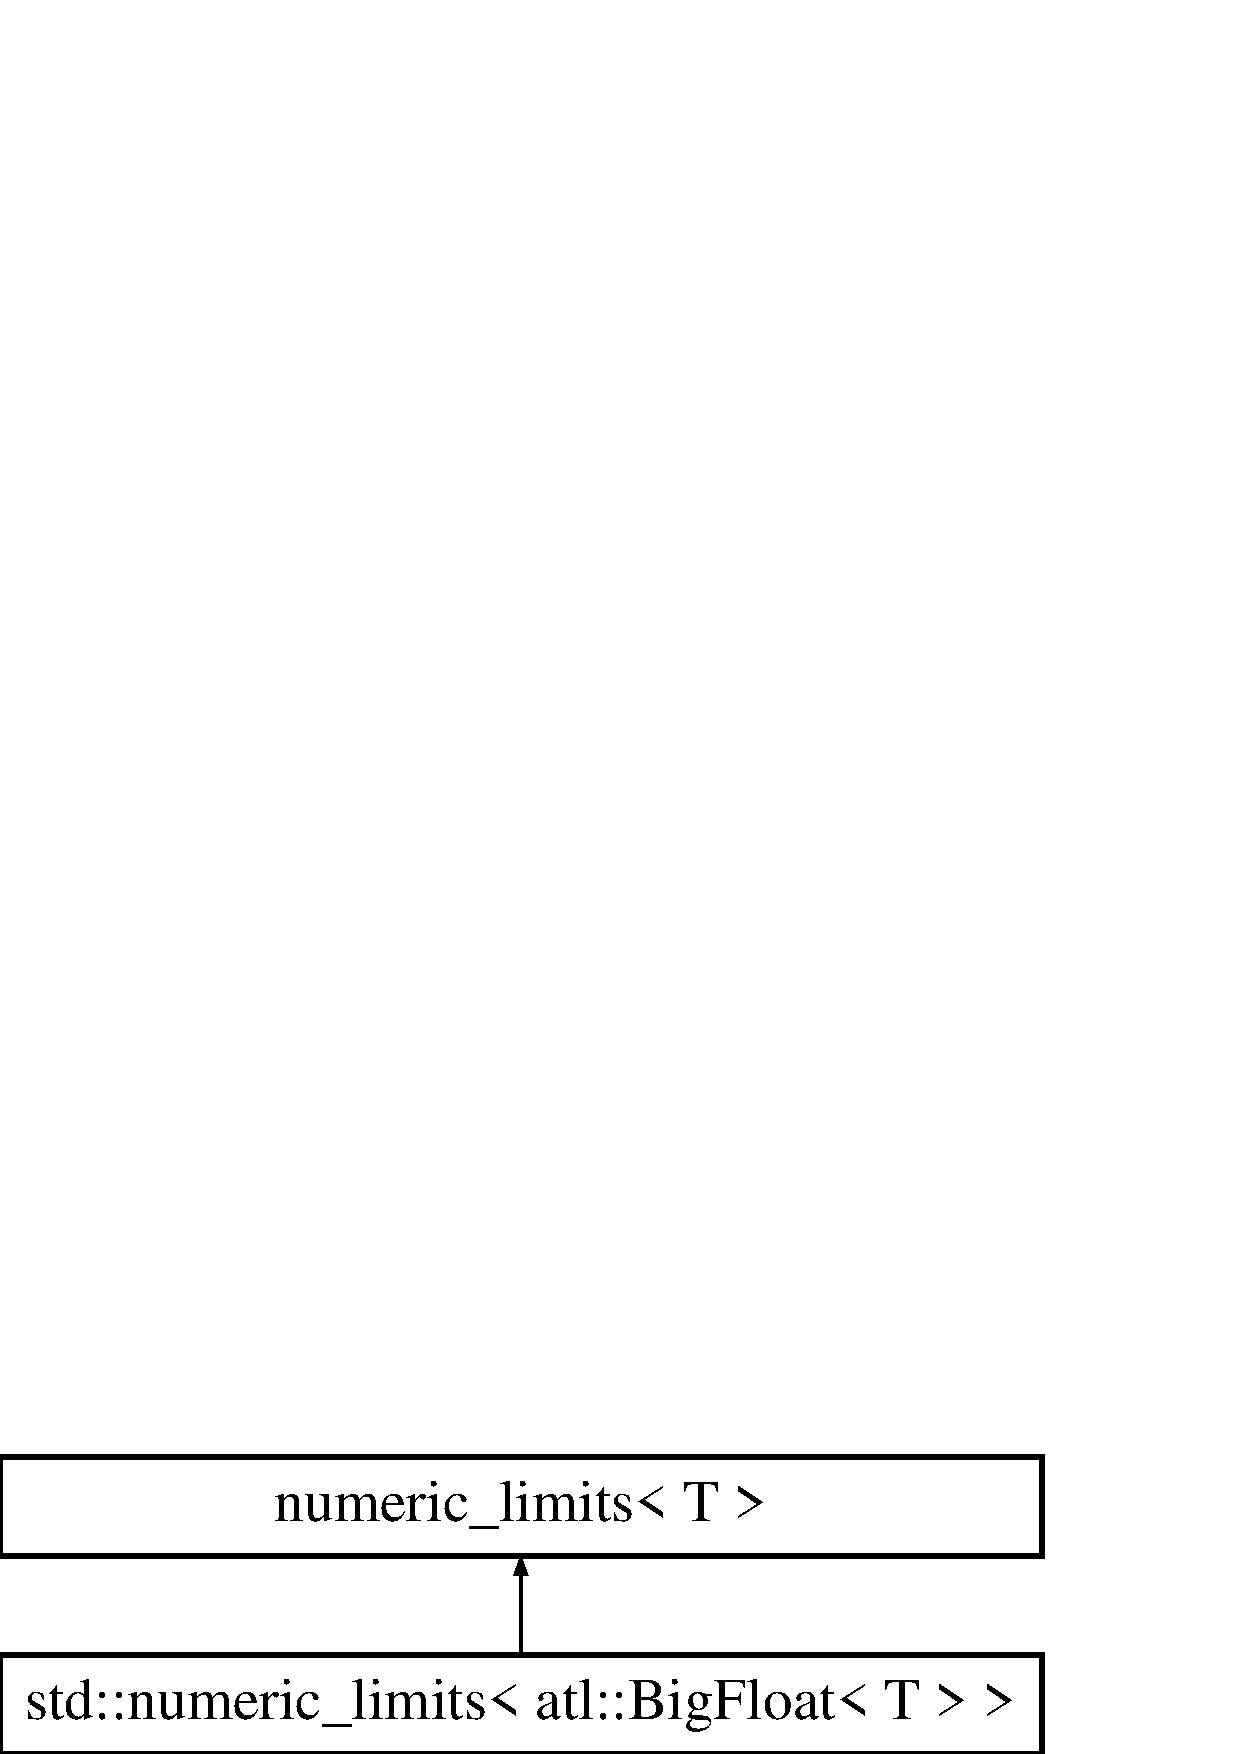
\includegraphics[height=2.000000cm]{classstd_1_1numeric__limits_3_01atl_1_1_big_float_3_01_t_01_4_01_4}
\end{center}
\end{figure}


The documentation for this class was generated from the following file\+:\begin{DoxyCompactItemize}
\item 
Utilities/Big\+Float.\+hpp\end{DoxyCompactItemize}

\hypertarget{structatl_1_1_pow}{\section{atl\+:\+:Pow$<$ R\+E\+A\+L\+\_\+\+T, L\+H\+S, R\+H\+S $>$ Struct Template Reference}
\label{structatl_1_1_pow}\index{atl\+::\+Pow$<$ R\+E\+A\+L\+\_\+\+T, L\+H\+S, R\+H\+S $>$@{atl\+::\+Pow$<$ R\+E\+A\+L\+\_\+\+T, L\+H\+S, R\+H\+S $>$}}
}


{\ttfamily \#include $<$Pow.\+hpp$>$}

Inheritance diagram for atl\+:\+:Pow$<$ R\+E\+A\+L\+\_\+\+T, L\+H\+S, R\+H\+S $>$\+:\begin{figure}[H]
\begin{center}
\leavevmode
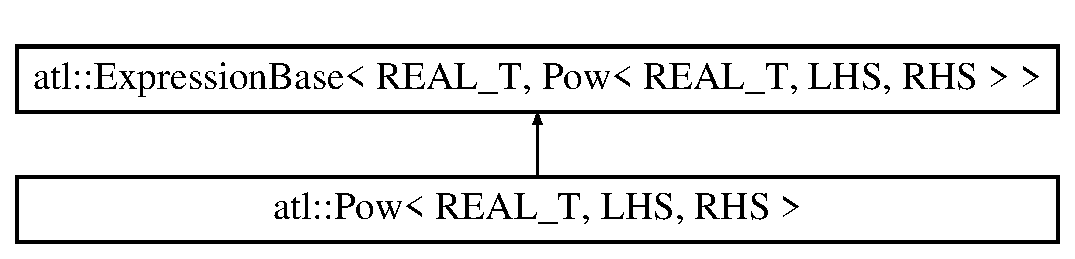
\includegraphics[height=2.000000cm]{structatl_1_1_pow}
\end{center}
\end{figure}
\subsection*{Public Types}
\begin{DoxyCompactItemize}
\item 
\hypertarget{structatl_1_1_pow_a8b99b01478601e39de33f01be84b68db}{typedef R\+E\+A\+L\+\_\+\+T {\bfseries B\+A\+S\+E\+\_\+\+T\+Y\+P\+E}}\label{structatl_1_1_pow_a8b99b01478601e39de33f01be84b68db}

\end{DoxyCompactItemize}
\subsection*{Public Member Functions}
\begin{DoxyCompactItemize}
\item 
\hyperlink{structatl_1_1_pow_afb3e80bbc1bbeb76ccd888329272662a}{Pow} (const \hyperlink{structatl_1_1_expression_base}{Expression\+Base}$<$ R\+E\+A\+L\+\_\+\+T, L\+H\+S $>$ \&lhs, const \hyperlink{structatl_1_1_expression_base}{Expression\+Base}$<$ R\+E\+A\+L\+\_\+\+T, R\+H\+S $>$ \&rhs)
\item 
\hyperlink{structatl_1_1_pow_ae955961ba2a3ca77c7b4270ac16de12c}{Pow} (const R\+E\+A\+L\+\_\+\+T \&lhs, const \hyperlink{structatl_1_1_expression_base}{Expression\+Base}$<$ R\+E\+A\+L\+\_\+\+T, R\+H\+S $>$ \&rhs)
\item 
\hyperlink{structatl_1_1_pow_ae463f403a238b2cf4343ae40ddd97da7}{Pow} (const \hyperlink{structatl_1_1_expression_base}{Expression\+Base}$<$ R\+E\+A\+L\+\_\+\+T, L\+H\+S $>$ \&lhs, const R\+E\+A\+L\+\_\+\+T \&rhs)
\item 
const R\+E\+A\+L\+\_\+\+T \hyperlink{structatl_1_1_pow_a7239d2c29b75f2cfac4a898c07bebdea}{Get\+Value} () const 
\item 
const R\+E\+A\+L\+\_\+\+T \hyperlink{structatl_1_1_pow_a40ce8705e527d1781ec0113922adbb8a}{Get\+Value} (size\+\_\+t i, size\+\_\+t j=0) const 
\item 
bool \hyperlink{structatl_1_1_pow_a0cc1139fdf06fc5022739df45ff02c07}{Is\+Nonlinear} () const 
\item 
void \hyperlink{structatl_1_1_pow_a57c5b681bfbdc13658d6ad8a4d58b6cd}{Push\+Ids} (typename \hyperlink{structatl_1_1_stack_entry}{atl\+::\+Stack\+Entry}$<$ R\+E\+A\+L\+\_\+\+T $>$\+::vi\+\_\+storage \&ids) const 
\item 
void \hyperlink{structatl_1_1_pow_ab5fa97cfa79b08f23a94b912bcb2178f}{Push\+Ids} (typename \hyperlink{structatl_1_1_stack_entry}{atl\+::\+Stack\+Entry}$<$ R\+E\+A\+L\+\_\+\+T $>$\+::vi\+\_\+storage \&ids, size\+\_\+t i, size\+\_\+t j=0) const 
\item 
R\+E\+A\+L\+\_\+\+T \hyperlink{structatl_1_1_pow_a9cb128cf177456cdd44d98146059545a}{Evaluate\+Derivative} (uint32\+\_\+t x) const 
\item 
R\+E\+A\+L\+\_\+\+T \hyperlink{structatl_1_1_pow_a9e9fddff89f3d2f3c134cb318c51d635}{Evaluate\+Derivative} (uint32\+\_\+t x, uint32\+\_\+t y) const 
\item 
R\+E\+A\+L\+\_\+\+T \hyperlink{structatl_1_1_pow_a2035cc8133459198476f2d082e9759ac}{Evaluate\+Derivative} (uint32\+\_\+t x, uint32\+\_\+t y, uint32\+\_\+t z) const 
\item 
R\+E\+A\+L\+\_\+\+T \hyperlink{structatl_1_1_pow_a9f3c0b19723d735fa733764006c84914}{Evaluate\+Derivative} (uint32\+\_\+t x, size\+\_\+t i, size\+\_\+t j=0) const 
\item 
R\+E\+A\+L\+\_\+\+T \hyperlink{structatl_1_1_pow_ac192ad0cdb7592038e0d4af6e735fe88}{Evaluate\+Derivative} (uint32\+\_\+t x, uint32\+\_\+t y, size\+\_\+t i, size\+\_\+t j=0) const 
\item 
R\+E\+A\+L\+\_\+\+T \hyperlink{structatl_1_1_pow_a337409b2b5e07d18b20458c59fa069f2}{Evaluate\+Derivative} (uint32\+\_\+t x, uint32\+\_\+t y, uint32\+\_\+t z, size\+\_\+t i, size\+\_\+t j=0) const 
\item 
size\+\_\+t \hyperlink{structatl_1_1_pow_a2ed5957f759a023657429d3a750f027a}{Get\+Columns} () const 
\item 
size\+\_\+t \hyperlink{structatl_1_1_pow_ab8184e894327ee2de4f6c6600a57344d}{Get\+Rows} () const 
\item 
bool \hyperlink{structatl_1_1_pow_a063b34eeb877161d1e24d358a179515c}{Is\+Scalar} () const 
\item 
const std\+::string \hyperlink{structatl_1_1_pow_acfc21ce83c00307ed77d575a263c15b5}{To\+Expression\+Template\+String} () const 
\end{DoxyCompactItemize}
\subsection*{Public Attributes}
\begin{DoxyCompactItemize}
\item 
\hypertarget{structatl_1_1_pow_ae8863f02dcc5b532addb5df805e89cfc}{\hyperlink{structatl_1_1_real}{atl\+::\+Real}$<$ R\+E\+A\+L\+\_\+\+T $>$ {\bfseries real\+\_\+m}}\label{structatl_1_1_pow_ae8863f02dcc5b532addb5df805e89cfc}

\item 
\hypertarget{structatl_1_1_pow_a303898c5af96f347781cf1b47a97f202}{const L\+H\+S \& {\bfseries lhs\+\_\+m}}\label{structatl_1_1_pow_a303898c5af96f347781cf1b47a97f202}

\item 
\hypertarget{structatl_1_1_pow_a74f0d6779873d6b336db9ad470370db2}{const R\+H\+S \& {\bfseries rhs\+\_\+m}}\label{structatl_1_1_pow_a74f0d6779873d6b336db9ad470370db2}

\item 
\hypertarget{structatl_1_1_pow_a3982a1d9d34c60425521448f2e06a0bb}{R\+E\+A\+L\+\_\+\+T {\bfseries value\+\_\+m}}\label{structatl_1_1_pow_a3982a1d9d34c60425521448f2e06a0bb}

\end{DoxyCompactItemize}


\subsection{Detailed Description}
\subsubsection*{template$<$class R\+E\+A\+L\+\_\+\+T, class L\+H\+S, class R\+H\+S$>$struct atl\+::\+Pow$<$ R\+E\+A\+L\+\_\+\+T, L\+H\+S, R\+H\+S $>$}

Expression template to handle pow for variable or container expressions.

$ f(x)^{g(x)} $

or

$ f_{i,j}(x)^{g_{i,j}(x)} $ 

\subsection{Constructor \& Destructor Documentation}
\hypertarget{structatl_1_1_pow_afb3e80bbc1bbeb76ccd888329272662a}{\index{atl\+::\+Pow@{atl\+::\+Pow}!Pow@{Pow}}
\index{Pow@{Pow}!atl\+::\+Pow@{atl\+::\+Pow}}
\subsubsection[{Pow}]{\setlength{\rightskip}{0pt plus 5cm}template$<$class R\+E\+A\+L\+\_\+\+T, class L\+H\+S , class R\+H\+S $>$ {\bf atl\+::\+Pow}$<$ R\+E\+A\+L\+\_\+\+T, L\+H\+S, R\+H\+S $>$\+::{\bf Pow} (
\begin{DoxyParamCaption}
\item[{const {\bf Expression\+Base}$<$ R\+E\+A\+L\+\_\+\+T, L\+H\+S $>$ \&}]{lhs, }
\item[{const {\bf Expression\+Base}$<$ R\+E\+A\+L\+\_\+\+T, R\+H\+S $>$ \&}]{rhs}
\end{DoxyParamCaption}
)\hspace{0.3cm}{\ttfamily [inline]}}}\label{structatl_1_1_pow_afb3e80bbc1bbeb76ccd888329272662a}
Constructor for two expression template types.


\begin{DoxyParams}{Parameters}
{\em lhs} & \\
\hline
{\em rhs} & \\
\hline
\end{DoxyParams}
\hypertarget{structatl_1_1_pow_ae955961ba2a3ca77c7b4270ac16de12c}{\index{atl\+::\+Pow@{atl\+::\+Pow}!Pow@{Pow}}
\index{Pow@{Pow}!atl\+::\+Pow@{atl\+::\+Pow}}
\subsubsection[{Pow}]{\setlength{\rightskip}{0pt plus 5cm}template$<$class R\+E\+A\+L\+\_\+\+T, class L\+H\+S , class R\+H\+S $>$ {\bf atl\+::\+Pow}$<$ R\+E\+A\+L\+\_\+\+T, L\+H\+S, R\+H\+S $>$\+::{\bf Pow} (
\begin{DoxyParamCaption}
\item[{const R\+E\+A\+L\+\_\+\+T \&}]{lhs, }
\item[{const {\bf Expression\+Base}$<$ R\+E\+A\+L\+\_\+\+T, R\+H\+S $>$ \&}]{rhs}
\end{DoxyParamCaption}
)\hspace{0.3cm}{\ttfamily [inline]}}}\label{structatl_1_1_pow_ae955961ba2a3ca77c7b4270ac16de12c}
Constructor for a real and expression template type.


\begin{DoxyParams}{Parameters}
{\em lhs} & \\
\hline
{\em rhs} & \\
\hline
\end{DoxyParams}
\hypertarget{structatl_1_1_pow_ae463f403a238b2cf4343ae40ddd97da7}{\index{atl\+::\+Pow@{atl\+::\+Pow}!Pow@{Pow}}
\index{Pow@{Pow}!atl\+::\+Pow@{atl\+::\+Pow}}
\subsubsection[{Pow}]{\setlength{\rightskip}{0pt plus 5cm}template$<$class R\+E\+A\+L\+\_\+\+T, class L\+H\+S , class R\+H\+S $>$ {\bf atl\+::\+Pow}$<$ R\+E\+A\+L\+\_\+\+T, L\+H\+S, R\+H\+S $>$\+::{\bf Pow} (
\begin{DoxyParamCaption}
\item[{const {\bf Expression\+Base}$<$ R\+E\+A\+L\+\_\+\+T, L\+H\+S $>$ \&}]{lhs, }
\item[{const R\+E\+A\+L\+\_\+\+T \&}]{rhs}
\end{DoxyParamCaption}
)\hspace{0.3cm}{\ttfamily [inline]}}}\label{structatl_1_1_pow_ae463f403a238b2cf4343ae40ddd97da7}
Constructor for a expression template type and a real type.


\begin{DoxyParams}{Parameters}
{\em lhs} & \\
\hline
{\em rhs} & \\
\hline
\end{DoxyParams}


\subsection{Member Function Documentation}
\hypertarget{structatl_1_1_pow_a9cb128cf177456cdd44d98146059545a}{\index{atl\+::\+Pow@{atl\+::\+Pow}!Evaluate\+Derivative@{Evaluate\+Derivative}}
\index{Evaluate\+Derivative@{Evaluate\+Derivative}!atl\+::\+Pow@{atl\+::\+Pow}}
\subsubsection[{Evaluate\+Derivative}]{\setlength{\rightskip}{0pt plus 5cm}template$<$class R\+E\+A\+L\+\_\+\+T, class L\+H\+S , class R\+H\+S $>$ R\+E\+A\+L\+\_\+\+T {\bf atl\+::\+Pow}$<$ R\+E\+A\+L\+\_\+\+T, L\+H\+S, R\+H\+S $>$\+::Evaluate\+Derivative (
\begin{DoxyParamCaption}
\item[{uint32\+\_\+t}]{x}
\end{DoxyParamCaption}
) const\hspace{0.3cm}{\ttfamily [inline]}}}\label{structatl_1_1_pow_a9cb128cf177456cdd44d98146059545a}
Evaluates the first-\/order derivative with respect to x.

$ f\left(x\right)^{g\left(x\right)}\,\left(\log f\left(x\right)\, \left({{d}\over{d\,x}}\,g\left(x\right)\right)+{{g\left(x\right)\, \left({{d}\over{d\,x}}\,f\left(x\right)\right)}\over{f\left(x\right) }}\right) $


\begin{DoxyParams}{Parameters}
{\em x} & \\
\hline
\end{DoxyParams}
\begin{DoxyReturn}{Returns}

\end{DoxyReturn}
\hypertarget{structatl_1_1_pow_a9e9fddff89f3d2f3c134cb318c51d635}{\index{atl\+::\+Pow@{atl\+::\+Pow}!Evaluate\+Derivative@{Evaluate\+Derivative}}
\index{Evaluate\+Derivative@{Evaluate\+Derivative}!atl\+::\+Pow@{atl\+::\+Pow}}
\subsubsection[{Evaluate\+Derivative}]{\setlength{\rightskip}{0pt plus 5cm}template$<$class R\+E\+A\+L\+\_\+\+T, class L\+H\+S , class R\+H\+S $>$ R\+E\+A\+L\+\_\+\+T {\bf atl\+::\+Pow}$<$ R\+E\+A\+L\+\_\+\+T, L\+H\+S, R\+H\+S $>$\+::Evaluate\+Derivative (
\begin{DoxyParamCaption}
\item[{uint32\+\_\+t}]{x, }
\item[{uint32\+\_\+t}]{y}
\end{DoxyParamCaption}
) const\hspace{0.3cm}{\ttfamily [inline]}}}\label{structatl_1_1_pow_a9e9fddff89f3d2f3c134cb318c51d635}
Evaluates the second-\/order derivative with respect to x and y.

$ f(x,y)^{g(x,y)}\,\left({{{{d}\over{d\,x}}\,f(x,y) \,\left({{d}\over{d\,y}}\,g(x,y)\right)}\over{f(x,y)}}+ \log f(x,y)\,\left({{d^2}\over{d\,x\,d\,y}}\,g(x,y) \right)+{{{{d}\over{d\,y}}\,f(x,y)\,\left({{d}\over{d\,x}}\,g (x,y)\right)}\over{f(x,y)}}-{{g(x,y)\,\left({{d }\over{d\,x}}\,f(x,y)\right)\,\left({{d}\over{d\,y}}\,f( x,y)\right)}\over{f(x,y)^2}}+ \\ {{g(x,y)\,\left({{d^2 }\over{d\,x\,d\,y}}\,f(x,y)\right)}\over{f(x,y)}}\right) +f(x,y)^{g(x,y)}\,\left(\log f(x,y)\,\left({{d }\over{d\,x}}\,g(x,y)\right)+{{g(x,y)\,\left({{d}\over{d \,x}}\,f(x,y)\right)}\over{f(x,y)}}\right)\,\left(\log f (x,y)\,\left({{d}\over{d\,y}}\,g(x,y)\right)+{{g(x ,y)\,\left({{d}\over{d\,y}}\,f(x,y)\right)}\over{f(x,y) }}\right) $


\begin{DoxyParams}{Parameters}
{\em x} & \\
\hline
{\em y} & \\
\hline
\end{DoxyParams}
\begin{DoxyReturn}{Returns}

\end{DoxyReturn}
\hypertarget{structatl_1_1_pow_a2035cc8133459198476f2d082e9759ac}{\index{atl\+::\+Pow@{atl\+::\+Pow}!Evaluate\+Derivative@{Evaluate\+Derivative}}
\index{Evaluate\+Derivative@{Evaluate\+Derivative}!atl\+::\+Pow@{atl\+::\+Pow}}
\subsubsection[{Evaluate\+Derivative}]{\setlength{\rightskip}{0pt plus 5cm}template$<$class R\+E\+A\+L\+\_\+\+T, class L\+H\+S , class R\+H\+S $>$ R\+E\+A\+L\+\_\+\+T {\bf atl\+::\+Pow}$<$ R\+E\+A\+L\+\_\+\+T, L\+H\+S, R\+H\+S $>$\+::Evaluate\+Derivative (
\begin{DoxyParamCaption}
\item[{uint32\+\_\+t}]{x, }
\item[{uint32\+\_\+t}]{y, }
\item[{uint32\+\_\+t}]{z}
\end{DoxyParamCaption}
) const\hspace{0.3cm}{\ttfamily [inline]}}}\label{structatl_1_1_pow_a2035cc8133459198476f2d082e9759ac}
Evaluates the third-\/order derivative with respect to x, y, and z.

$f(x,y,z)^{g(x,y,z)}\,\left(-{{{{d}\over{d\,x}}\,f (x,y,z)\,\left({{d}\over{d\,y}}\,f(x,y,z)\right)\,\left({{d }\over{d\,z}}\,g(x,y,z)\right)}\over{f(x,y,z)^2}}+{{{{d^ 2}\over{d\,x\,d\,y}}\,f(x,y,z)\,\left({{d}\over{d\,z}}\,g_{i,j }(x,y,z)\right)}\over{f(x,y,z)}}+{{{{d}\over{d\,x}}\,f(x ,y,z)\,\left({{d^2}\over{d\,y\,d\,z}}\,g(x,y,z)\right)}\over{f (x,y,z)}}-{{{{d}\over{d\,x}}\,f(x,y,z)\,\left({{d}\over{ d\,z}}\,f(x,y,z)\right)\,\left({{d}\over{d\,y}}\,g(x,y,z )\right)}\over{f(x,y,z)^2}}+ \\ {{{{d^2}\over{d\,x\,d\,z}}\,f_{i,j }(x,y,z)\,\left({{d}\over{d\,y}}\,g(x,y,z)\right)}\over{f_{i,j }(x,y,z)}}+{{{{d}\over{d\,y}}\,f(x,y,z)\,\left({{d^2}\over{d\, x\,d\,z}}\,g(x,y,z)\right)}\over{f(x,y,z)}}+\log f (x,y,z)\,\left({{d^3}\over{d\,x\,d\,y\,d\,z}}\,g(x,y,z)\right) +{{{{d}\over{d\,z}}\,f(x,y,z)\,\left({{d^2}\over{d\,x\,d\,y}} \,g(x,y,z)\right)}\over{f(x,y,z)}}-{{{{d}\over{d\,y}}\,f (x,y,z)\,\left({{d}\over{d\,z}}\,f(x,y,z)\right)\,\left( {{d}\over{d\,x}}\,g(x,y,z)\right)}\over{f(x,y,z)^2}}+{{ {{d^2}\over{d\,y\,d\,z}}\,f(x,y,z)\,\left({{d}\over{d\,x}}\,g (x,y,z)\right)}\over{f(x,y,z)}}+ \\ {{2\,g(x,y,z)\, \left({{d}\over{d\,x}}\,f(x,y,z)\right)\,\left({{d}\over{d\,y }}\,f(x,y,z)\right)\,\left({{d}\over{d\,z}}\,f(x,y,z) \right)}\over{f(x,y,z)^3}}-{{g(x,y,z)\,\left({{d^2 }\over{d\,x\,d\,y}}\,f(x,y,z)\right)\,\left({{d}\over{d\,z}}\, f(x,y,z)\right)}\over{f(x,y,z)^2}}-{{g(x,y,z)\, \left({{d}\over{d\,x}}\,f(x,y,z)\right)\,\left({{d^2}\over{d\, y\,d\,z}}\,f(x,y,z)\right)}\over{f(x,y,z)^2}}-{{g( x,y,z)\,\left({{d^2}\over{d\,x\,d\,z}}\,f(x,y,z)\right)\, \left({{d}\over{d\,y}}\,f(x,y,z)\right)}\over{f(x,y,z)^2 }}+{{g(x,y,z)\,\left({{d^3}\over{d\,x\,d\,y\,d\,z}}\,f(x ,y,z)\right)}\over{f(x,y,z)}}\right)+ \\ f(x,y,z)^{g(x ,y,z)}\,\left(\log f(x,y,z)\,\left({{d}\over{d\,x}}\,g(x ,y,z)\right)+{{g(x,y,z)\,\left({{d}\over{d\,x}}\,f(x,y,z )\right)}\over{f(x,y,z)}}\right)\,\left({{{{d}\over{d\,y}}\,f (x,y,z)\,\left({{d}\over{d\,z}}\,g(x,y,z)\right)}\over{f (x,y,z)}}+\log f(x,y,z)\,\left({{d^2}\over{d\,y\,d\,z}} \,g(x,y,z)\right)+{{{{d}\over{d\,z}}\,f(x,y,z)\,\left({{ d}\over{d\,y}}\,g(x,y,z)\right)}\over{f(x,y,z)}}-{{g_{i, j}(x,y,z)\,\left({{d}\over{d\,y}}\,f(x,y,z)\right)\,\left({{d }\over{d\,z}}\,f(x,y,z)\right)}\over{f(x,y,z)^2}}+{{g_{i ,j}(x,y,z)\,\left({{d^2}\over{d\,y\,d\,z}}\,f(x,y,z)\right) }\over{f(x,y,z)}}\right)+ \\ f(x,y,z)^{g(x,y,z)}\, \left(\log f(x,y,z)\,\left({{d}\over{d\,y}}\,g(x,y,z) \right)+{{g(x,y,z)\,\left({{d}\over{d\,y}}\,f(x,y,z) \right)}\over{f(x,y,z)}}\right)\,\left({{{{d}\over{d\,x}}\,f_{ i,j}(x,y,z)\,\left({{d}\over{d\,z}}\,g(x,y,z)\right)}\over{f_{ i,j}(x,y,z)}}+\log f(x,y,z)\,\left({{d^2}\over{d\,x\,d\,z}}\,g (x,y,z)\right)+{{{{d}\over{d\,z}}\,f(x,y,z)\,\left({{d }\over{d\,x}}\,g(x,y,z)\right)}\over{f(x,y,z)}}-{{g_{i,j }(x,y,z)\,\left({{d}\over{d\,x}}\,f(x,y,z)\right)\,\left({{d }\over{d\,z}}\,f(x,y,z)\right)}\over{f(x,y,z)^2}}+{{g_{i ,j}(x,y,z)\,\left({{d^2}\over{d\,x\,d\,z}}\,f(x,y,z)\right) }\over{f(x,y,z)}}\right)+ \\ f(x,y,z)^{g(x,y,z)}\, \left({{{{d}\over{d\,x}}\,f(x,y,z)\,\left({{d}\over{d\,y}}\,g (x,y,z)\right)}\over{f(x,y,z)}}+\log f(x,y,z)\, \left({{d^2}\over{d\,x\,d\,y}}\,g(x,y,z)\right)+{{{{d}\over{d \,y}}\,f(x,y,z)\,\left({{d}\over{d\,x}}\,g(x,y,z)\right) }\over{f(x,y,z)}}-{{g(x,y,z)\,\left({{d}\over{d\,x}}\,f (x,y,z)\right)\,\left({{d}\over{d\,y}}\,f(x,y,z)\right) }\over{f(x,y,z)^2}}+{{g(x,y,z)\,\left({{d^2}\over{d\,x\, d\,y}}\,f(x,y,z)\right)}\over{f(x,y,z)}}\right)\,\left( \log f(x,y,z)\,\left({{d}\over{d\,z}}\,g(x,y,z)\right)+ {{g(x,y,z)\,\left({{d}\over{d\,z}}\,f(x,y,z)\right) }\over{f(x,y,z)}}\right)+ \\ f(x,y,z)^{g(x,y,z)}\, \left(\log f(x,y,z)\,\left({{d}\over{d\,x}}\,g(x,y,z) \right)+{{g(x,y,z)\,\left({{d}\over{d\,x}}\,f(x,y,z) \right)}\over{f(x,y,z)}}\right)\,\left(\log f(x,y,z)\, \left({{d}\over{d\,y}}\,g(x,y,z)\right)+{{g(x,y,z)\, \left({{d}\over{d\,y}}\,f(x,y,z)\right)}\over{f(x,y,z)}} \right)\,\left(\log f(x,y,z)\,\left({{d}\over{d\,z}}\,g( x,y,z)\right)+{{g(x,y,z)\,\left({{d}\over{d\,z}}\,f(x,y, z)\right)}\over{f(x,y,z)}}\right) $


\begin{DoxyParams}{Parameters}
{\em x} & \\
\hline
{\em y} & \\
\hline
{\em z} & \\
\hline
\end{DoxyParams}
\begin{DoxyReturn}{Returns}

\end{DoxyReturn}
\hypertarget{structatl_1_1_pow_a9f3c0b19723d735fa733764006c84914}{\index{atl\+::\+Pow@{atl\+::\+Pow}!Evaluate\+Derivative@{Evaluate\+Derivative}}
\index{Evaluate\+Derivative@{Evaluate\+Derivative}!atl\+::\+Pow@{atl\+::\+Pow}}
\subsubsection[{Evaluate\+Derivative}]{\setlength{\rightskip}{0pt plus 5cm}template$<$class R\+E\+A\+L\+\_\+\+T, class L\+H\+S , class R\+H\+S $>$ R\+E\+A\+L\+\_\+\+T {\bf atl\+::\+Pow}$<$ R\+E\+A\+L\+\_\+\+T, L\+H\+S, R\+H\+S $>$\+::Evaluate\+Derivative (
\begin{DoxyParamCaption}
\item[{uint32\+\_\+t}]{x, }
\item[{size\+\_\+t}]{i, }
\item[{size\+\_\+t}]{j = {\ttfamily 0}}
\end{DoxyParamCaption}
) const\hspace{0.3cm}{\ttfamily [inline]}}}\label{structatl_1_1_pow_a9f3c0b19723d735fa733764006c84914}
Evaluates the first-\/order derivative with respect to x at index \{i,j\}.

$ f_{i,j}(x)^{g_{i,j}(x)}\,\left(\log f_{i,j}(x)\,\left({{d}\over{d\, x}}\,g_{i,j}(x)\right)+{{g_{i,j}(x)\,\left({{d}\over{d\,x}}\,f_{i,j} (x)\right)}\over{f_{i,j}(x)}}\right) $


\begin{DoxyParams}{Parameters}
{\em x} & \\
\hline
{\em i} & \\
\hline
{\em j} & \\
\hline
\end{DoxyParams}
\begin{DoxyReturn}{Returns}

\end{DoxyReturn}
\hypertarget{structatl_1_1_pow_ac192ad0cdb7592038e0d4af6e735fe88}{\index{atl\+::\+Pow@{atl\+::\+Pow}!Evaluate\+Derivative@{Evaluate\+Derivative}}
\index{Evaluate\+Derivative@{Evaluate\+Derivative}!atl\+::\+Pow@{atl\+::\+Pow}}
\subsubsection[{Evaluate\+Derivative}]{\setlength{\rightskip}{0pt plus 5cm}template$<$class R\+E\+A\+L\+\_\+\+T, class L\+H\+S , class R\+H\+S $>$ R\+E\+A\+L\+\_\+\+T {\bf atl\+::\+Pow}$<$ R\+E\+A\+L\+\_\+\+T, L\+H\+S, R\+H\+S $>$\+::Evaluate\+Derivative (
\begin{DoxyParamCaption}
\item[{uint32\+\_\+t}]{x, }
\item[{uint32\+\_\+t}]{y, }
\item[{size\+\_\+t}]{i, }
\item[{size\+\_\+t}]{j = {\ttfamily 0}}
\end{DoxyParamCaption}
) const\hspace{0.3cm}{\ttfamily [inline]}}}\label{structatl_1_1_pow_ac192ad0cdb7592038e0d4af6e735fe88}
Evaluates the second-\/order derivative with respect to x and y at index \{i,j\}.

$ f_{i,j}(x,y)^{g_{i,j}(x,y)}\,\left({{{{d}\over{d\,x}}\,f_{i,j}(x,y) \,\left({{d}\over{d\,y}}\,g_{i,j}(x,y)\right)}\over{f_{i,j}(x,y)}}+ \log f_{i,j}(x,y)\,\left({{d^2}\over{d\,x\,d\,y}}\,g_{i,j}(x,y) \right)+{{{{d}\over{d\,y}}\,f_{i,j}(x,y)\,\left({{d}\over{d\,x}}\,g _{i,j}(x,y)\right)}\over{f_{i,j}(x,y)}}-{{g_{i,j}(x,y)\,\left({{d }\over{d\,x}}\,f_{i,j}(x,y)\right)\,\left({{d}\over{d\,y}}\,f_{i,j}( x,y)\right)}\over{f_{i,j}(x,y)^2}}+ \\ {{g_{i,j}(x,y)\,\left({{d^2 }\over{d\,x\,d\,y}}\,f_{i,j}(x,y)\right)}\over{f_{i,j}(x,y)}}\right) +f_{i,j}(x,y)^{g_{i,j}(x,y)}\,\left(\log f_{i,j}(x,y)\,\left({{d }\over{d\,x}}\,g_{i,j}(x,y)\right)+{{g_{i,j}(x,y)\,\left({{d}\over{d \,x}}\,f_{i,j}(x,y)\right)}\over{f_{i,j}(x,y)}}\right)\,\left(\log f _{i,j}(x,y)\,\left({{d}\over{d\,y}}\,g_{i,j}(x,y)\right)+{{g_{i,j}(x ,y)\,\left({{d}\over{d\,y}}\,f_{i,j}(x,y)\right)}\over{f_{i,j}(x,y) }}\right) $


\begin{DoxyParams}{Parameters}
{\em x} & \\
\hline
{\em y} & \\
\hline
{\em i} & \\
\hline
{\em j} & \\
\hline
\end{DoxyParams}
\begin{DoxyReturn}{Returns}

\end{DoxyReturn}
\hypertarget{structatl_1_1_pow_a337409b2b5e07d18b20458c59fa069f2}{\index{atl\+::\+Pow@{atl\+::\+Pow}!Evaluate\+Derivative@{Evaluate\+Derivative}}
\index{Evaluate\+Derivative@{Evaluate\+Derivative}!atl\+::\+Pow@{atl\+::\+Pow}}
\subsubsection[{Evaluate\+Derivative}]{\setlength{\rightskip}{0pt plus 5cm}template$<$class R\+E\+A\+L\+\_\+\+T, class L\+H\+S , class R\+H\+S $>$ R\+E\+A\+L\+\_\+\+T {\bf atl\+::\+Pow}$<$ R\+E\+A\+L\+\_\+\+T, L\+H\+S, R\+H\+S $>$\+::Evaluate\+Derivative (
\begin{DoxyParamCaption}
\item[{uint32\+\_\+t}]{x, }
\item[{uint32\+\_\+t}]{y, }
\item[{uint32\+\_\+t}]{z, }
\item[{size\+\_\+t}]{i, }
\item[{size\+\_\+t}]{j = {\ttfamily 0}}
\end{DoxyParamCaption}
) const\hspace{0.3cm}{\ttfamily [inline]}}}\label{structatl_1_1_pow_a337409b2b5e07d18b20458c59fa069f2}
Evaluates the third-\/order derivative with respect to x, y, and z at index \{i,j\}.

$f_{i,j}(x,y,z)^{g_{i,j}(x,y,z)}\,\left(-{{{{d}\over{d\,x}}\,f_{i,j} (x,y,z)\,\left({{d}\over{d\,y}}\,f_{i,j}(x,y,z)\right)\,\left({{d }\over{d\,z}}\,g_{i,j}(x,y,z)\right)}\over{f_{i,j}(x,y,z)^2}}+{{{{d^ 2}\over{d\,x\,d\,y}}\,f_{i,j}(x,y,z)\,\left({{d}\over{d\,z}}\,g_{i,j }(x,y,z)\right)}\over{f_{i,j}(x,y,z)}}+{{{{d}\over{d\,x}}\,f_{i,j}(x ,y,z)\,\left({{d^2}\over{d\,y\,d\,z}}\,g_{i,j}(x,y,z)\right)}\over{f _{i,j}(x,y,z)}}-{{{{d}\over{d\,x}}\,f_{i,j}(x,y,z)\,\left({{d}\over{ d\,z}}\,f_{i,j}(x,y,z)\right)\,\left({{d}\over{d\,y}}\,g_{i,j}(x,y,z )\right)}\over{f_{i,j}(x,y,z)^2}}+ \\ {{{{d^2}\over{d\,x\,d\,z}}\,f_{i,j }(x,y,z)\,\left({{d}\over{d\,y}}\,g_{i,j}(x,y,z)\right)}\over{f_{i,j }(x,y,z)}}+{{{{d}\over{d\,y}}\,f_{i,j}(x,y,z)\,\left({{d^2}\over{d\, x\,d\,z}}\,g_{i,j}(x,y,z)\right)}\over{f_{i,j}(x,y,z)}}+\log f_{i,j} (x,y,z)\,\left({{d^3}\over{d\,x\,d\,y\,d\,z}}\,g_{i,j}(x,y,z)\right) +{{{{d}\over{d\,z}}\,f_{i,j}(x,y,z)\,\left({{d^2}\over{d\,x\,d\,y}} \,g_{i,j}(x,y,z)\right)}\over{f_{i,j}(x,y,z)}}-{{{{d}\over{d\,y}}\,f _{i,j}(x,y,z)\,\left({{d}\over{d\,z}}\,f_{i,j}(x,y,z)\right)\,\left( {{d}\over{d\,x}}\,g_{i,j}(x,y,z)\right)}\over{f_{i,j}(x,y,z)^2}}+{{ {{d^2}\over{d\,y\,d\,z}}\,f_{i,j}(x,y,z)\,\left({{d}\over{d\,x}}\,g _{i,j}(x,y,z)\right)}\over{f_{i,j}(x,y,z)}}+ \\ {{2\,g_{i,j}(x,y,z)\, \left({{d}\over{d\,x}}\,f_{i,j}(x,y,z)\right)\,\left({{d}\over{d\,y }}\,f_{i,j}(x,y,z)\right)\,\left({{d}\over{d\,z}}\,f_{i,j}(x,y,z) \right)}\over{f_{i,j}(x,y,z)^3}}-{{g_{i,j}(x,y,z)\,\left({{d^2 }\over{d\,x\,d\,y}}\,f_{i,j}(x,y,z)\right)\,\left({{d}\over{d\,z}}\, f_{i,j}(x,y,z)\right)}\over{f_{i,j}(x,y,z)^2}}-{{g_{i,j}(x,y,z)\, \left({{d}\over{d\,x}}\,f_{i,j}(x,y,z)\right)\,\left({{d^2}\over{d\, y\,d\,z}}\,f_{i,j}(x,y,z)\right)}\over{f_{i,j}(x,y,z)^2}}-{{g_{i,j}( x,y,z)\,\left({{d^2}\over{d\,x\,d\,z}}\,f_{i,j}(x,y,z)\right)\, \left({{d}\over{d\,y}}\,f_{i,j}(x,y,z)\right)}\over{f_{i,j}(x,y,z)^2 }}+{{g_{i,j}(x,y,z)\,\left({{d^3}\over{d\,x\,d\,y\,d\,z}}\,f_{i,j}(x ,y,z)\right)}\over{f_{i,j}(x,y,z)}}\right)+ \\ f_{i,j}(x,y,z)^{g_{i,j}(x ,y,z)}\,\left(\log f_{i,j}(x,y,z)\,\left({{d}\over{d\,x}}\,g_{i,j}(x ,y,z)\right)+{{g_{i,j}(x,y,z)\,\left({{d}\over{d\,x}}\,f_{i,j}(x,y,z )\right)}\over{f_{i,j}(x,y,z)}}\right)\,\left({{{{d}\over{d\,y}}\,f _{i,j}(x,y,z)\,\left({{d}\over{d\,z}}\,g_{i,j}(x,y,z)\right)}\over{f _{i,j}(x,y,z)}}+\log f_{i,j}(x,y,z)\,\left({{d^2}\over{d\,y\,d\,z}} \,g_{i,j}(x,y,z)\right)+{{{{d}\over{d\,z}}\,f_{i,j}(x,y,z)\,\left({{ d}\over{d\,y}}\,g_{i,j}(x,y,z)\right)}\over{f_{i,j}(x,y,z)}}-{{g_{i, j}(x,y,z)\,\left({{d}\over{d\,y}}\,f_{i,j}(x,y,z)\right)\,\left({{d }\over{d\,z}}\,f_{i,j}(x,y,z)\right)}\over{f_{i,j}(x,y,z)^2}}+{{g_{i ,j}(x,y,z)\,\left({{d^2}\over{d\,y\,d\,z}}\,f_{i,j}(x,y,z)\right) }\over{f_{i,j}(x,y,z)}}\right)+ \\ f_{i,j}(x,y,z)^{g_{i,j}(x,y,z)}\, \left(\log f_{i,j}(x,y,z)\,\left({{d}\over{d\,y}}\,g_{i,j}(x,y,z) \right)+{{g_{i,j}(x,y,z)\,\left({{d}\over{d\,y}}\,f_{i,j}(x,y,z) \right)}\over{f_{i,j}(x,y,z)}}\right)\,\left({{{{d}\over{d\,x}}\,f_{ i,j}(x,y,z)\,\left({{d}\over{d\,z}}\,g_{i,j}(x,y,z)\right)}\over{f_{ i,j}(x,y,z)}}+\log f_{i,j}(x,y,z)\,\left({{d^2}\over{d\,x\,d\,z}}\,g _{i,j}(x,y,z)\right)+{{{{d}\over{d\,z}}\,f_{i,j}(x,y,z)\,\left({{d }\over{d\,x}}\,g_{i,j}(x,y,z)\right)}\over{f_{i,j}(x,y,z)}}-{{g_{i,j }(x,y,z)\,\left({{d}\over{d\,x}}\,f_{i,j}(x,y,z)\right)\,\left({{d }\over{d\,z}}\,f_{i,j}(x,y,z)\right)}\over{f_{i,j}(x,y,z)^2}}+{{g_{i ,j}(x,y,z)\,\left({{d^2}\over{d\,x\,d\,z}}\,f_{i,j}(x,y,z)\right) }\over{f_{i,j}(x,y,z)}}\right)+ \\ f_{i,j}(x,y,z)^{g_{i,j}(x,y,z)}\, \left({{{{d}\over{d\,x}}\,f_{i,j}(x,y,z)\,\left({{d}\over{d\,y}}\,g _{i,j}(x,y,z)\right)}\over{f_{i,j}(x,y,z)}}+\log f_{i,j}(x,y,z)\, \left({{d^2}\over{d\,x\,d\,y}}\,g_{i,j}(x,y,z)\right)+{{{{d}\over{d \,y}}\,f_{i,j}(x,y,z)\,\left({{d}\over{d\,x}}\,g_{i,j}(x,y,z)\right) }\over{f_{i,j}(x,y,z)}}-{{g_{i,j}(x,y,z)\,\left({{d}\over{d\,x}}\,f _{i,j}(x,y,z)\right)\,\left({{d}\over{d\,y}}\,f_{i,j}(x,y,z)\right) }\over{f_{i,j}(x,y,z)^2}}+{{g_{i,j}(x,y,z)\,\left({{d^2}\over{d\,x\, d\,y}}\,f_{i,j}(x,y,z)\right)}\over{f_{i,j}(x,y,z)}}\right)\,\left( \log f_{i,j}(x,y,z)\,\left({{d}\over{d\,z}}\,g_{i,j}(x,y,z)\right)+ {{g_{i,j}(x,y,z)\,\left({{d}\over{d\,z}}\,f_{i,j}(x,y,z)\right) }\over{f_{i,j}(x,y,z)}}\right)+ \\ f_{i,j}(x,y,z)^{g_{i,j}(x,y,z)}\, \left(\log f_{i,j}(x,y,z)\,\left({{d}\over{d\,x}}\,g_{i,j}(x,y,z) \right)+{{g_{i,j}(x,y,z)\,\left({{d}\over{d\,x}}\,f_{i,j}(x,y,z) \right)}\over{f_{i,j}(x,y,z)}}\right)\,\left(\log f_{i,j}(x,y,z)\, \left({{d}\over{d\,y}}\,g_{i,j}(x,y,z)\right)+{{g_{i,j}(x,y,z)\, \left({{d}\over{d\,y}}\,f_{i,j}(x,y,z)\right)}\over{f_{i,j}(x,y,z)}} \right)\,\left(\log f_{i,j}(x,y,z)\,\left({{d}\over{d\,z}}\,g_{i,j}( x,y,z)\right)+{{g_{i,j}(x,y,z)\,\left({{d}\over{d\,z}}\,f_{i,j}(x,y, z)\right)}\over{f_{i,j}(x,y,z)}}\right) $


\begin{DoxyParams}{Parameters}
{\em x} & \\
\hline
{\em y} & \\
\hline
{\em z} & \\
\hline
{\em i} & \\
\hline
{\em j} & \\
\hline
\end{DoxyParams}
\begin{DoxyReturn}{Returns}

\end{DoxyReturn}
\hypertarget{structatl_1_1_pow_a2ed5957f759a023657429d3a750f027a}{\index{atl\+::\+Pow@{atl\+::\+Pow}!Get\+Columns@{Get\+Columns}}
\index{Get\+Columns@{Get\+Columns}!atl\+::\+Pow@{atl\+::\+Pow}}
\subsubsection[{Get\+Columns}]{\setlength{\rightskip}{0pt plus 5cm}template$<$class R\+E\+A\+L\+\_\+\+T, class L\+H\+S , class R\+H\+S $>$ size\+\_\+t {\bf atl\+::\+Pow}$<$ R\+E\+A\+L\+\_\+\+T, L\+H\+S, R\+H\+S $>$\+::Get\+Columns (
\begin{DoxyParamCaption}
{}
\end{DoxyParamCaption}
) const\hspace{0.3cm}{\ttfamily [inline]}}}\label{structatl_1_1_pow_a2ed5957f759a023657429d3a750f027a}
Returns the number of columns.

\begin{DoxyReturn}{Returns}

\end{DoxyReturn}
\hypertarget{structatl_1_1_pow_ab8184e894327ee2de4f6c6600a57344d}{\index{atl\+::\+Pow@{atl\+::\+Pow}!Get\+Rows@{Get\+Rows}}
\index{Get\+Rows@{Get\+Rows}!atl\+::\+Pow@{atl\+::\+Pow}}
\subsubsection[{Get\+Rows}]{\setlength{\rightskip}{0pt plus 5cm}template$<$class R\+E\+A\+L\+\_\+\+T, class L\+H\+S , class R\+H\+S $>$ size\+\_\+t {\bf atl\+::\+Pow}$<$ R\+E\+A\+L\+\_\+\+T, L\+H\+S, R\+H\+S $>$\+::Get\+Rows (
\begin{DoxyParamCaption}
{}
\end{DoxyParamCaption}
) const\hspace{0.3cm}{\ttfamily [inline]}}}\label{structatl_1_1_pow_ab8184e894327ee2de4f6c6600a57344d}
Returns the number of rows.

\begin{DoxyReturn}{Returns}

\end{DoxyReturn}
\hypertarget{structatl_1_1_pow_a7239d2c29b75f2cfac4a898c07bebdea}{\index{atl\+::\+Pow@{atl\+::\+Pow}!Get\+Value@{Get\+Value}}
\index{Get\+Value@{Get\+Value}!atl\+::\+Pow@{atl\+::\+Pow}}
\subsubsection[{Get\+Value}]{\setlength{\rightskip}{0pt plus 5cm}template$<$class R\+E\+A\+L\+\_\+\+T, class L\+H\+S , class R\+H\+S $>$ const R\+E\+A\+L\+\_\+\+T {\bf atl\+::\+Pow}$<$ R\+E\+A\+L\+\_\+\+T, L\+H\+S, R\+H\+S $>$\+::Get\+Value (
\begin{DoxyParamCaption}
{}
\end{DoxyParamCaption}
) const\hspace{0.3cm}{\ttfamily [inline]}}}\label{structatl_1_1_pow_a7239d2c29b75f2cfac4a898c07bebdea}
Computes the the evaluation of the lhs raised by the evaluation of the rhs.

\begin{DoxyReturn}{Returns}

\end{DoxyReturn}
\hypertarget{structatl_1_1_pow_a40ce8705e527d1781ec0113922adbb8a}{\index{atl\+::\+Pow@{atl\+::\+Pow}!Get\+Value@{Get\+Value}}
\index{Get\+Value@{Get\+Value}!atl\+::\+Pow@{atl\+::\+Pow}}
\subsubsection[{Get\+Value}]{\setlength{\rightskip}{0pt plus 5cm}template$<$class R\+E\+A\+L\+\_\+\+T, class L\+H\+S , class R\+H\+S $>$ const R\+E\+A\+L\+\_\+\+T {\bf atl\+::\+Pow}$<$ R\+E\+A\+L\+\_\+\+T, L\+H\+S, R\+H\+S $>$\+::Get\+Value (
\begin{DoxyParamCaption}
\item[{size\+\_\+t}]{i, }
\item[{size\+\_\+t}]{j = {\ttfamily 0}}
\end{DoxyParamCaption}
) const\hspace{0.3cm}{\ttfamily [inline]}}}\label{structatl_1_1_pow_a40ce8705e527d1781ec0113922adbb8a}
Computes the the evaluation of the lhs raised by the evaluation of the rhs at index \{i,j\}.

\begin{DoxyReturn}{Returns}

\end{DoxyReturn}
\hypertarget{structatl_1_1_pow_a0cc1139fdf06fc5022739df45ff02c07}{\index{atl\+::\+Pow@{atl\+::\+Pow}!Is\+Nonlinear@{Is\+Nonlinear}}
\index{Is\+Nonlinear@{Is\+Nonlinear}!atl\+::\+Pow@{atl\+::\+Pow}}
\subsubsection[{Is\+Nonlinear}]{\setlength{\rightskip}{0pt plus 5cm}template$<$class R\+E\+A\+L\+\_\+\+T, class L\+H\+S , class R\+H\+S $>$ bool {\bf atl\+::\+Pow}$<$ R\+E\+A\+L\+\_\+\+T, L\+H\+S, R\+H\+S $>$\+::Is\+Nonlinear (
\begin{DoxyParamCaption}
{}
\end{DoxyParamCaption}
) const\hspace{0.3cm}{\ttfamily [inline]}}}\label{structatl_1_1_pow_a0cc1139fdf06fc5022739df45ff02c07}
Returns true.

\begin{DoxyReturn}{Returns}

\end{DoxyReturn}
\hypertarget{structatl_1_1_pow_a063b34eeb877161d1e24d358a179515c}{\index{atl\+::\+Pow@{atl\+::\+Pow}!Is\+Scalar@{Is\+Scalar}}
\index{Is\+Scalar@{Is\+Scalar}!atl\+::\+Pow@{atl\+::\+Pow}}
\subsubsection[{Is\+Scalar}]{\setlength{\rightskip}{0pt plus 5cm}template$<$class R\+E\+A\+L\+\_\+\+T, class L\+H\+S , class R\+H\+S $>$ bool {\bf atl\+::\+Pow}$<$ R\+E\+A\+L\+\_\+\+T, L\+H\+S, R\+H\+S $>$\+::Is\+Scalar (
\begin{DoxyParamCaption}
{}
\end{DoxyParamCaption}
) const\hspace{0.3cm}{\ttfamily [inline]}}}\label{structatl_1_1_pow_a063b34eeb877161d1e24d358a179515c}
True if scalar.

\begin{DoxyReturn}{Returns}

\end{DoxyReturn}
\hypertarget{structatl_1_1_pow_a57c5b681bfbdc13658d6ad8a4d58b6cd}{\index{atl\+::\+Pow@{atl\+::\+Pow}!Push\+Ids@{Push\+Ids}}
\index{Push\+Ids@{Push\+Ids}!atl\+::\+Pow@{atl\+::\+Pow}}
\subsubsection[{Push\+Ids}]{\setlength{\rightskip}{0pt plus 5cm}template$<$class R\+E\+A\+L\+\_\+\+T, class L\+H\+S , class R\+H\+S $>$ void {\bf atl\+::\+Pow}$<$ R\+E\+A\+L\+\_\+\+T, L\+H\+S, R\+H\+S $>$\+::Push\+Ids (
\begin{DoxyParamCaption}
\item[{typename {\bf atl\+::\+Stack\+Entry}$<$ R\+E\+A\+L\+\_\+\+T $>$\+::vi\+\_\+storage \&}]{ids}
\end{DoxyParamCaption}
) const\hspace{0.3cm}{\ttfamily [inline]}}}\label{structatl_1_1_pow_a57c5b681bfbdc13658d6ad8a4d58b6cd}
Push ids into a set.


\begin{DoxyParams}{Parameters}
{\em ids} & \\
\hline
\end{DoxyParams}
\hypertarget{structatl_1_1_pow_ab5fa97cfa79b08f23a94b912bcb2178f}{\index{atl\+::\+Pow@{atl\+::\+Pow}!Push\+Ids@{Push\+Ids}}
\index{Push\+Ids@{Push\+Ids}!atl\+::\+Pow@{atl\+::\+Pow}}
\subsubsection[{Push\+Ids}]{\setlength{\rightskip}{0pt plus 5cm}template$<$class R\+E\+A\+L\+\_\+\+T, class L\+H\+S , class R\+H\+S $>$ void {\bf atl\+::\+Pow}$<$ R\+E\+A\+L\+\_\+\+T, L\+H\+S, R\+H\+S $>$\+::Push\+Ids (
\begin{DoxyParamCaption}
\item[{typename {\bf atl\+::\+Stack\+Entry}$<$ R\+E\+A\+L\+\_\+\+T $>$\+::vi\+\_\+storage \&}]{ids, }
\item[{size\+\_\+t}]{i, }
\item[{size\+\_\+t}]{j = {\ttfamily 0}}
\end{DoxyParamCaption}
) const\hspace{0.3cm}{\ttfamily [inline]}}}\label{structatl_1_1_pow_ab5fa97cfa79b08f23a94b912bcb2178f}
Push ids into a set at index \{i,j\}.


\begin{DoxyParams}{Parameters}
{\em ids} & \\
\hline
{\em i} & \\
\hline
{\em j} & \\
\hline
\end{DoxyParams}
\hypertarget{structatl_1_1_pow_acfc21ce83c00307ed77d575a263c15b5}{\index{atl\+::\+Pow@{atl\+::\+Pow}!To\+Expression\+Template\+String@{To\+Expression\+Template\+String}}
\index{To\+Expression\+Template\+String@{To\+Expression\+Template\+String}!atl\+::\+Pow@{atl\+::\+Pow}}
\subsubsection[{To\+Expression\+Template\+String}]{\setlength{\rightskip}{0pt plus 5cm}template$<$class R\+E\+A\+L\+\_\+\+T, class L\+H\+S , class R\+H\+S $>$ const std\+::string {\bf atl\+::\+Pow}$<$ R\+E\+A\+L\+\_\+\+T, L\+H\+S, R\+H\+S $>$\+::To\+Expression\+Template\+String (
\begin{DoxyParamCaption}
{}
\end{DoxyParamCaption}
) const\hspace{0.3cm}{\ttfamily [inline]}}}\label{structatl_1_1_pow_acfc21ce83c00307ed77d575a263c15b5}
Create a string representation of this expression template. \begin{DoxyReturn}{Returns}

\end{DoxyReturn}


The documentation for this struct was generated from the following file\+:\begin{DoxyCompactItemize}
\item 
Pow.\+hpp\end{DoxyCompactItemize}

\hypertarget{structprocheap}{\section{procheap Struct Reference}
\label{structprocheap}\index{procheap@{procheap}}
}
\subsection*{Public Attributes}
\begin{DoxyCompactItemize}
\item 
\hypertarget{structprocheap_a16dafd9789a76a53b1a7696df8947081}{\hyperlink{structdesc}{desc\+\_\+t} $\ast$volatile {\bfseries Active}}\label{structprocheap_a16dafd9789a76a53b1a7696df8947081}

\item 
\hypertarget{structprocheap_a11dffb3df6d76b5d0446fcb1ce26ba9b}{\hyperlink{structdesc}{desc\+\_\+t} $\ast$volatile {\bfseries Partial}}\label{structprocheap_a11dffb3df6d76b5d0446fcb1ce26ba9b}

\item 
\hypertarget{structprocheap_a28e29b2c5769fbd68050f6082902a3d3}{struct \hyperlink{structsizeclass}{sizeclass} $\ast$ {\bfseries sc}}\label{structprocheap_a28e29b2c5769fbd68050f6082902a3d3}

\item 
\hypertarget{structprocheap_ad520cbc7a4ccc75eb1f09da379c43e76}{char {\bfseries pad} \mbox{[}32-\/3 $\ast$sizeof(void $\ast$)\mbox{]}}\label{structprocheap_ad520cbc7a4ccc75eb1f09da379c43e76}

\end{DoxyCompactItemize}


The documentation for this struct was generated from the following file\+:\begin{DoxyCompactItemize}
\item 
A\+T\+L2/clfmalloc.\+h\end{DoxyCompactItemize}

\hypertarget{structprofile__entry______}{\section{profile\+\_\+entry\+\_\+\+\_\+\+\_\+ Struct Reference}
\label{structprofile__entry______}\index{profile\+\_\+entry\+\_\+\+\_\+\+\_\+@{profile\+\_\+entry\+\_\+\+\_\+\+\_\+}}
}
\subsection*{Public Member Functions}
\begin{DoxyCompactItemize}
\item 
\hypertarget{structprofile__entry_______ab67daf5a84320a08e44d8d87139d59d6}{{\bfseries profile\+\_\+entry\+\_\+\+\_\+\+\_\+} (std\+::string function\+\_\+name)}\label{structprofile__entry_______ab67daf5a84320a08e44d8d87139d59d6}

\end{DoxyCompactItemize}
\subsection*{Public Attributes}
\begin{DoxyCompactItemize}
\item 
\hypertarget{structprofile__entry_______afe7a4c63f9bced4f5f9bd6bfa5d74557}{std\+::string {\bfseries function\+\_\+name}}\label{structprofile__entry_______afe7a4c63f9bced4f5f9bd6bfa5d74557}

\item 
\hypertarget{structprofile__entry_______a4a5554b80ae414599d61e40929d13019}{std\+::chrono\+::high\+\_\+resolution\+\_\+clock\+::time\+\_\+point {\bfseries start}}\label{structprofile__entry_______a4a5554b80ae414599d61e40929d13019}

\item 
\hypertarget{structprofile__entry_______a13e8d02839195369484346dc785298df}{std\+::chrono\+::high\+\_\+resolution\+\_\+clock\+::time\+\_\+point {\bfseries end}}\label{structprofile__entry_______a13e8d02839195369484346dc785298df}

\item 
\hypertarget{structprofile__entry_______ab2398e4192a3275b44ca28752d3cd0ef}{double {\bfseries total}}\label{structprofile__entry_______ab2398e4192a3275b44ca28752d3cd0ef}

\end{DoxyCompactItemize}


The documentation for this struct was generated from the following file\+:\begin{DoxyCompactItemize}
\item 
Utilities/Profile.\+hpp\end{DoxyCompactItemize}

\hypertarget{classtools_1_1_profiled_function}{\section{tools\+:\+:Profiled\+Function Class Reference}
\label{classtools_1_1_profiled_function}\index{tools\+::\+Profiled\+Function@{tools\+::\+Profiled\+Function}}
}
\subsection*{Public Member Functions}
\begin{DoxyCompactItemize}
\item 
\hypertarget{classtools_1_1_profiled_function_adddd217edca9578f05fa5fe9ac6a516c}{{\bfseries Profiled\+Function} (std\+::string name)}\label{classtools_1_1_profiled_function_adddd217edca9578f05fa5fe9ac6a516c}

\item 
\hypertarget{classtools_1_1_profiled_function_a08b2e4125c16ae08de420a3319450c27}{unsigned long {\bfseries Get\+Calls\+\_\+} () const }\label{classtools_1_1_profiled_function_a08b2e4125c16ae08de420a3319450c27}

\item 
\hypertarget{classtools_1_1_profiled_function_a6acda1004ef92051cf29f250b3d88112}{void {\bfseries Set\+Calls\+\_\+} (unsigned long calls\+\_\+)}\label{classtools_1_1_profiled_function_a6acda1004ef92051cf29f250b3d88112}

\item 
\hypertarget{classtools_1_1_profiled_function_aaeb9958400ec2b608f1ba07bf318bf74}{std\+::string {\bfseries Get\+Name\+\_\+} () const }\label{classtools_1_1_profiled_function_aaeb9958400ec2b608f1ba07bf318bf74}

\item 
\hypertarget{classtools_1_1_profiled_function_ad4f29ccbd8d6c4ba4cc634393e759155}{void {\bfseries Set\+Name\+\_\+} (std\+::string name\+\_\+)}\label{classtools_1_1_profiled_function_ad4f29ccbd8d6c4ba4cc634393e759155}

\item 
\hypertarget{classtools_1_1_profiled_function_a36acb5f61af96dff784b7e93e1523ffb}{double {\bfseries Get\+Time\+\_\+} () const }\label{classtools_1_1_profiled_function_a36acb5f61af96dff784b7e93e1523ffb}

\item 
\hypertarget{classtools_1_1_profiled_function_a40f012a139c5488abcde00011ce205a4}{void {\bfseries Set\+Time\+\_\+} (double time\+\_\+)}\label{classtools_1_1_profiled_function_a40f012a139c5488abcde00011ce205a4}

\item 
\hypertarget{classtools_1_1_profiled_function_a769ad7f606d86a3fe5aa314c8f0e7507}{void {\bfseries Start\+Timing} ()}\label{classtools_1_1_profiled_function_a769ad7f606d86a3fe5aa314c8f0e7507}

\item 
\hypertarget{classtools_1_1_profiled_function_ad63c5b2301953bccea9fb2e57ace99cd}{void {\bfseries Stop\+Timing} ()}\label{classtools_1_1_profiled_function_ad63c5b2301953bccea9fb2e57ace99cd}

\item 
\hypertarget{classtools_1_1_profiled_function_ad6467dbe52289e6d40d767fa9db04378}{double {\bfseries Get\+Average\+Time} ()}\label{classtools_1_1_profiled_function_ad6467dbe52289e6d40d767fa9db04378}

\end{DoxyCompactItemize}


The documentation for this class was generated from the following file\+:\begin{DoxyCompactItemize}
\item 
Utilities/Profiler.\+hpp\end{DoxyCompactItemize}

\hypertarget{structatl_1_1_real}{\section{atl\+:\+:Real$<$ R\+E\+A\+L\+\_\+\+T $>$ Struct Template Reference}
\label{structatl_1_1_real}\index{atl\+::\+Real$<$ R\+E\+A\+L\+\_\+\+T $>$@{atl\+::\+Real$<$ R\+E\+A\+L\+\_\+\+T $>$}}
}


{\ttfamily \#include $<$Real.\+hpp$>$}

Inheritance diagram for atl\+:\+:Real$<$ R\+E\+A\+L\+\_\+\+T $>$\+:\begin{figure}[H]
\begin{center}
\leavevmode
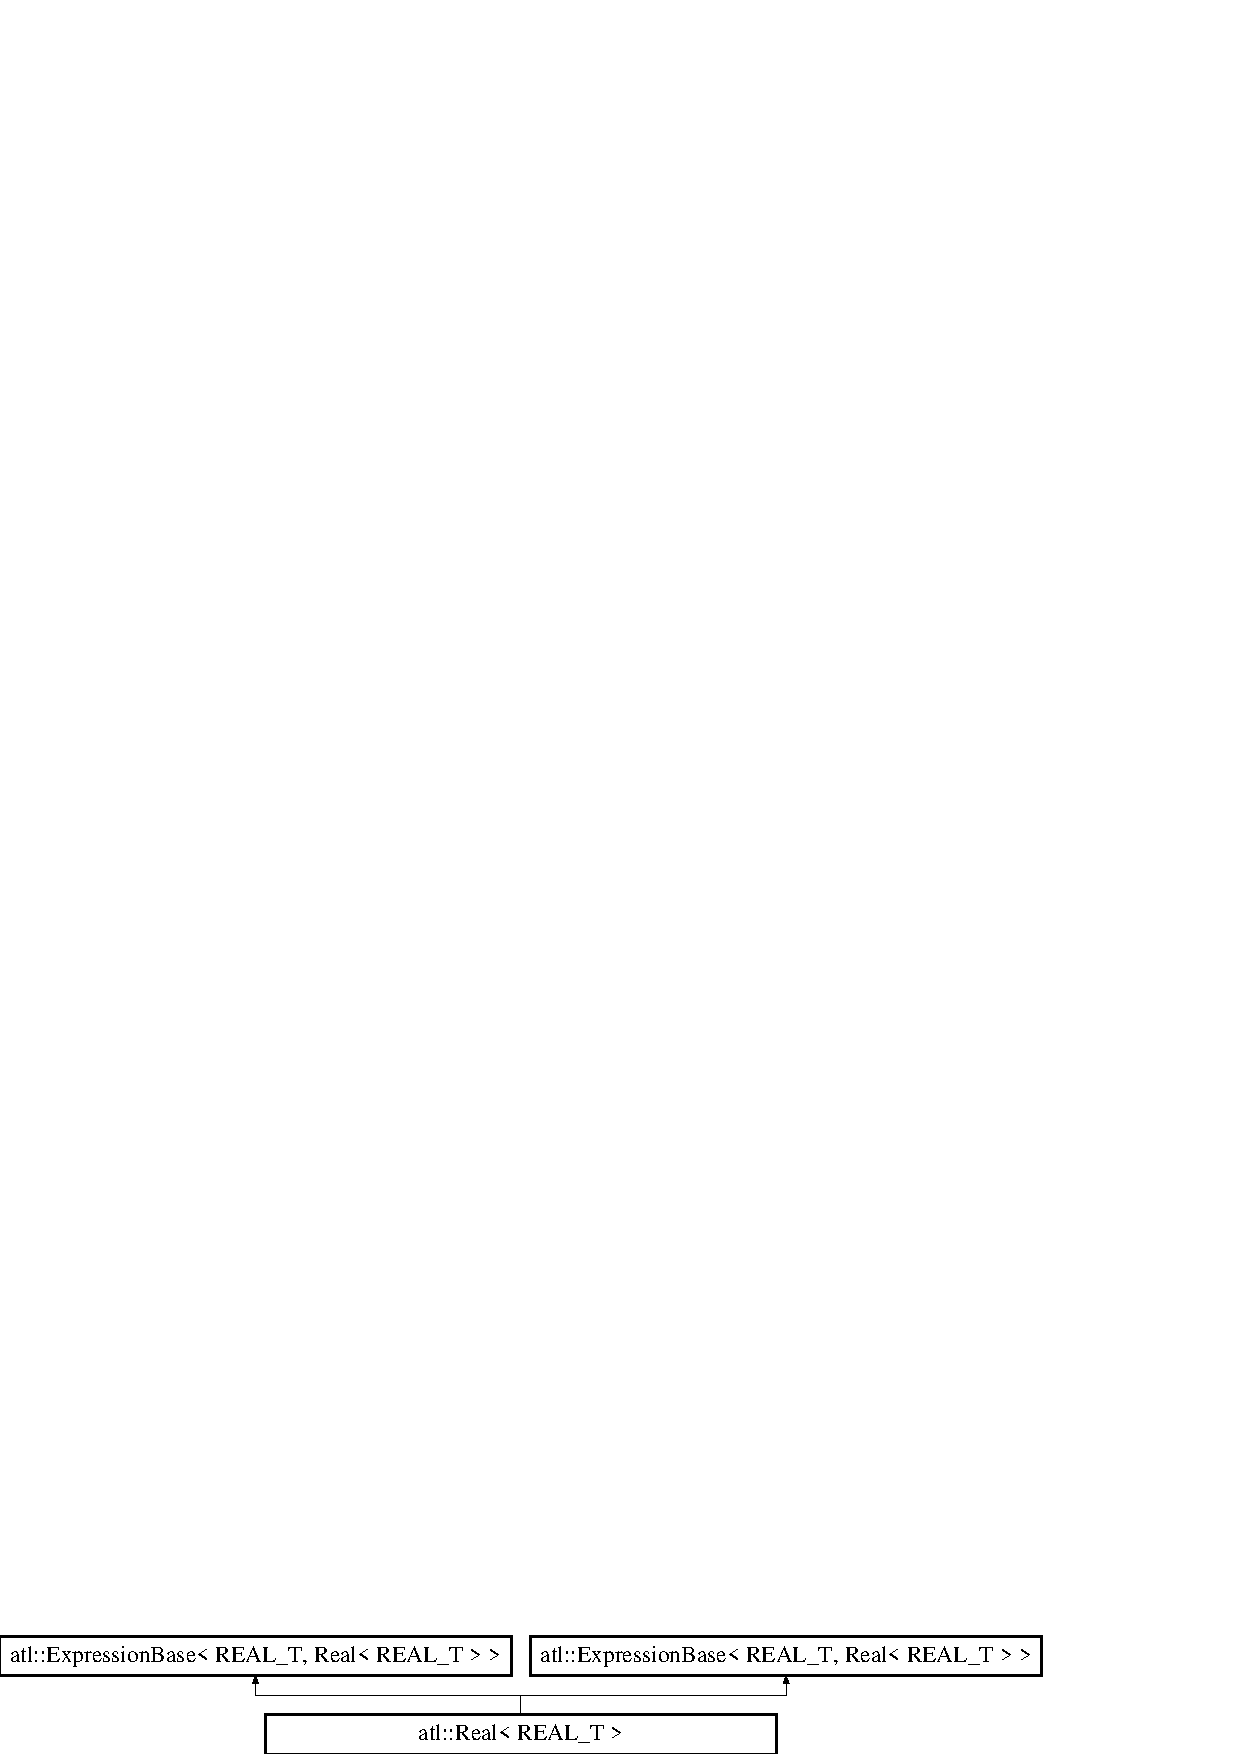
\includegraphics[height=1.848185cm]{structatl_1_1_real}
\end{center}
\end{figure}
\subsection*{Public Types}
\begin{DoxyCompactItemize}
\item 
\hypertarget{structatl_1_1_real_a777fa3a51746bde9ee8f79ffe26ace07}{typedef R\+E\+A\+L\+\_\+\+T {\bfseries base\+\_\+type}}\label{structatl_1_1_real_a777fa3a51746bde9ee8f79ffe26ace07}

\item 
\hypertarget{structatl_1_1_real_a777fa3a51746bde9ee8f79ffe26ace07}{typedef R\+E\+A\+L\+\_\+\+T {\bfseries base\+\_\+type}}\label{structatl_1_1_real_a777fa3a51746bde9ee8f79ffe26ace07}

\end{DoxyCompactItemize}
\subsection*{Public Member Functions}
\begin{DoxyCompactItemize}
\item 
\hypertarget{structatl_1_1_real_a3ef54e5b25ee5800cb9cc3a6702e54c2}{{\bfseries Real} (R\+E\+A\+L\+\_\+\+T v=static\+\_\+cast$<$ R\+E\+A\+L\+\_\+\+T $>$(0.\+0))}\label{structatl_1_1_real_a3ef54e5b25ee5800cb9cc3a6702e54c2}

\item 
\hypertarget{structatl_1_1_real_abdc6f5cef7138b4699f6405eed513864}{{\bfseries Real} (const \hyperlink{structatl_1_1_real}{Real}$<$ R\+E\+A\+L\+\_\+\+T $>$ \&other)}\label{structatl_1_1_real_abdc6f5cef7138b4699f6405eed513864}

\item 
\hypertarget{structatl_1_1_real_ab0ff33ff7cb2b6b75e69c50e648ae780}{\hyperlink{structatl_1_1_real}{Real} \& {\bfseries operator=} (const R\+E\+A\+L\+\_\+\+T \&v)}\label{structatl_1_1_real_ab0ff33ff7cb2b6b75e69c50e648ae780}

\item 
\hypertarget{structatl_1_1_real_a18df517fb08814575164e6d87cf637bc}{{\bfseries operator R\+E\+A\+L\+\_\+\+T} () const }\label{structatl_1_1_real_a18df517fb08814575164e6d87cf637bc}

\item 
\hypertarget{structatl_1_1_real_a2f5cb2f25c49951421acad1bf3acf340}{const R\+E\+A\+L\+\_\+\+T {\bfseries Get\+Value} () const }\label{structatl_1_1_real_a2f5cb2f25c49951421acad1bf3acf340}

\item 
\hypertarget{structatl_1_1_real_a6e8a09189115773e192963fc2a2ade8e}{const R\+E\+A\+L\+\_\+\+T {\bfseries Get\+Value} (size\+\_\+t i, size\+\_\+t j=0) const }\label{structatl_1_1_real_a6e8a09189115773e192963fc2a2ade8e}

\item 
\hypertarget{structatl_1_1_real_a5cb2b8223c6214ab4e157dd0d7f1a13e}{void {\bfseries Push\+Ids} (typename \hyperlink{structatl_1_1_stack_entry}{atl\+::\+Stack\+Entry}$<$ R\+E\+A\+L\+\_\+\+T $>$\+::vi\+\_\+storage \&ids) const }\label{structatl_1_1_real_a5cb2b8223c6214ab4e157dd0d7f1a13e}

\item 
\hypertarget{structatl_1_1_real_ae34aba11b0da584a407b7d02ac6631be}{void {\bfseries Push\+Ids} (typename \hyperlink{structatl_1_1_stack_entry}{atl\+::\+Stack\+Entry}$<$ R\+E\+A\+L\+\_\+\+T $>$\+::vi\+\_\+storage \&ids, size\+\_\+t i, size\+\_\+t j=0) const }\label{structatl_1_1_real_ae34aba11b0da584a407b7d02ac6631be}

\item 
\hypertarget{structatl_1_1_real_acbef29bf2238df385f08a79b64cd3f3e}{R\+E\+A\+L\+\_\+\+T {\bfseries Evaluate\+Derivative} (uint32\+\_\+t a) const }\label{structatl_1_1_real_acbef29bf2238df385f08a79b64cd3f3e}

\item 
\hypertarget{structatl_1_1_real_a75fa81c177d900427ed653422c954608}{R\+E\+A\+L\+\_\+\+T {\bfseries Evaluate\+Derivative} (uint32\+\_\+t a, uint32\+\_\+t b) const }\label{structatl_1_1_real_a75fa81c177d900427ed653422c954608}

\item 
\hypertarget{structatl_1_1_real_a1815b6e0510f3bf2a3f58f8a8c4191af}{R\+E\+A\+L\+\_\+\+T {\bfseries Evaluate\+Derivative} (uint32\+\_\+t x, uint32\+\_\+t y, uint32\+\_\+t z) const }\label{structatl_1_1_real_a1815b6e0510f3bf2a3f58f8a8c4191af}

\item 
\hypertarget{structatl_1_1_real_a6dc54d71b585d8120345d45f07d169f6}{R\+E\+A\+L\+\_\+\+T {\bfseries Evaluate\+Derivative} (uint32\+\_\+t a, size\+\_\+t i, size\+\_\+t j=0) const }\label{structatl_1_1_real_a6dc54d71b585d8120345d45f07d169f6}

\item 
\hypertarget{structatl_1_1_real_a7b0cc98e36edb3212be66d01c2b759b4}{R\+E\+A\+L\+\_\+\+T {\bfseries Evaluate\+Derivative} (uint32\+\_\+t a, uint32\+\_\+t b, size\+\_\+t i, size\+\_\+t j=0) const }\label{structatl_1_1_real_a7b0cc98e36edb3212be66d01c2b759b4}

\item 
\hypertarget{structatl_1_1_real_a9af356095d17f7173d85d8850159ecdc}{R\+E\+A\+L\+\_\+\+T {\bfseries Evaluate\+Derivative} (uint32\+\_\+t x, uint32\+\_\+t y, uint32\+\_\+t z, size\+\_\+t i, size\+\_\+t j=0) const }\label{structatl_1_1_real_a9af356095d17f7173d85d8850159ecdc}

\item 
\hypertarget{structatl_1_1_real_af08c2cd5341fa39e461c13251191081c}{size\+\_\+t {\bfseries Get\+Columns} () const }\label{structatl_1_1_real_af08c2cd5341fa39e461c13251191081c}

\item 
\hypertarget{structatl_1_1_real_a70d87c955e5b4566387b614ee6e81b6e}{size\+\_\+t {\bfseries Get\+Rows} () const }\label{structatl_1_1_real_a70d87c955e5b4566387b614ee6e81b6e}

\item 
\hypertarget{structatl_1_1_real_afa844d891d764e1ac8d0e78cccb78615}{bool {\bfseries Is\+Scalar} () const }\label{structatl_1_1_real_afa844d891d764e1ac8d0e78cccb78615}

\item 
\hyperlink{structatl_1_1_real_a3ef54e5b25ee5800cb9cc3a6702e54c2}{Real} (R\+E\+A\+L\+\_\+\+T v=static\+\_\+cast$<$ R\+E\+A\+L\+\_\+\+T $>$(0.\+0))
\item 
\hyperlink{structatl_1_1_real_abdc6f5cef7138b4699f6405eed513864}{Real} (const \hyperlink{structatl_1_1_real}{Real}$<$ R\+E\+A\+L\+\_\+\+T $>$ \&other)
\item 
\hyperlink{structatl_1_1_real}{Real} \& \hyperlink{structatl_1_1_real_ab0ff33ff7cb2b6b75e69c50e648ae780}{operator=} (const R\+E\+A\+L\+\_\+\+T \&v)
\item 
\hypertarget{structatl_1_1_real_a18df517fb08814575164e6d87cf637bc}{{\bfseries operator R\+E\+A\+L\+\_\+\+T} () const }\label{structatl_1_1_real_a18df517fb08814575164e6d87cf637bc}

\item 
const R\+E\+A\+L\+\_\+\+T \hyperlink{structatl_1_1_real_a2f5cb2f25c49951421acad1bf3acf340}{Get\+Value} () const 
\item 
const R\+E\+A\+L\+\_\+\+T \hyperlink{structatl_1_1_real_a6e8a09189115773e192963fc2a2ade8e}{Get\+Value} (size\+\_\+t i, size\+\_\+t j=0) const 
\item 
bool \hyperlink{structatl_1_1_real_add21737b5353260d88f2e828a44e3379}{Is\+Nonlinear} () const 
\item 
void \hyperlink{structatl_1_1_real_a5cb2b8223c6214ab4e157dd0d7f1a13e}{Push\+Ids} (typename \hyperlink{structatl_1_1_stack_entry}{atl\+::\+Stack\+Entry}$<$ R\+E\+A\+L\+\_\+\+T $>$\+::vi\+\_\+storage \&ids) const 
\item 
void \hyperlink{structatl_1_1_real_ae34aba11b0da584a407b7d02ac6631be}{Push\+Ids} (typename \hyperlink{structatl_1_1_stack_entry}{atl\+::\+Stack\+Entry}$<$ R\+E\+A\+L\+\_\+\+T $>$\+::vi\+\_\+storage \&ids, size\+\_\+t i, size\+\_\+t j=0) const 
\item 
R\+E\+A\+L\+\_\+\+T \hyperlink{structatl_1_1_real_aba08db5acde1f3de89cc5ac4d5c56055}{Evaluate\+Derivative} (uint32\+\_\+t x) const 
\item 
R\+E\+A\+L\+\_\+\+T \hyperlink{structatl_1_1_real_ac066173dcb25893acc9f76b3aca19180}{Evaluate\+Derivative} (uint32\+\_\+t x, uint32\+\_\+t y) const 
\item 
R\+E\+A\+L\+\_\+\+T \hyperlink{structatl_1_1_real_a1815b6e0510f3bf2a3f58f8a8c4191af}{Evaluate\+Derivative} (uint32\+\_\+t x, uint32\+\_\+t y, uint32\+\_\+t z) const 
\item 
R\+E\+A\+L\+\_\+\+T \hyperlink{structatl_1_1_real_a6a94daa6db6842f4df3d4e5072e0cba0}{Evaluate\+Derivative} (uint32\+\_\+t x, size\+\_\+t i, size\+\_\+t j=0) const 
\item 
R\+E\+A\+L\+\_\+\+T \hyperlink{structatl_1_1_real_a38575ddce1aa16e993c3739cef91eb85}{Evaluate\+Derivative} (uint32\+\_\+t x, uint32\+\_\+t y, size\+\_\+t i, size\+\_\+t j=0) const 
\item 
R\+E\+A\+L\+\_\+\+T \hyperlink{structatl_1_1_real_a9af356095d17f7173d85d8850159ecdc}{Evaluate\+Derivative} (uint32\+\_\+t x, uint32\+\_\+t y, uint32\+\_\+t z, size\+\_\+t i, size\+\_\+t j=0) const 
\item 
size\+\_\+t \hyperlink{structatl_1_1_real_af08c2cd5341fa39e461c13251191081c}{Get\+Columns} () const 
\item 
size\+\_\+t \hyperlink{structatl_1_1_real_a70d87c955e5b4566387b614ee6e81b6e}{Get\+Rows} () const 
\item 
bool \hyperlink{structatl_1_1_real_afa844d891d764e1ac8d0e78cccb78615}{Is\+Scalar} () const 
\item 
const std\+::string \hyperlink{structatl_1_1_real_a49866acc5c3a74eb4b57da139d702901}{To\+Expression\+Template\+String} () const 
\end{DoxyCompactItemize}
\subsection*{Public Attributes}
\begin{DoxyCompactItemize}
\item 
\hypertarget{structatl_1_1_real_a4de36acb39ddc2a51f5bf72421240152}{R\+E\+A\+L\+\_\+\+T {\bfseries value}}\label{structatl_1_1_real_a4de36acb39ddc2a51f5bf72421240152}

\end{DoxyCompactItemize}


\subsection{Detailed Description}
\subsubsection*{template$<$typename R\+E\+A\+L\+\_\+\+T$>$struct atl\+::\+Real$<$ R\+E\+A\+L\+\_\+\+T $>$}

Wrapper class for real numbers. Used in expression templates to avoid separate templates for operations involving real values in binary expressions. 

\subsection{Constructor \& Destructor Documentation}
\hypertarget{structatl_1_1_real_a3ef54e5b25ee5800cb9cc3a6702e54c2}{\index{atl\+::\+Real@{atl\+::\+Real}!Real@{Real}}
\index{Real@{Real}!atl\+::\+Real@{atl\+::\+Real}}
\subsubsection[{Real}]{\setlength{\rightskip}{0pt plus 5cm}template$<$typename R\+E\+A\+L\+\_\+\+T$>$ {\bf atl\+::\+Real}$<$ R\+E\+A\+L\+\_\+\+T $>$\+::{\bf Real} (
\begin{DoxyParamCaption}
\item[{R\+E\+A\+L\+\_\+\+T}]{v = {\ttfamily static\+\_\+cast$<$REAL\+\_\+T$>$~(0.0)}}
\end{DoxyParamCaption}
)\hspace{0.3cm}{\ttfamily [inline]}}}\label{structatl_1_1_real_a3ef54e5b25ee5800cb9cc3a6702e54c2}
Constructor.


\begin{DoxyParams}{Parameters}
{\em v} & \\
\hline
\end{DoxyParams}
\hypertarget{structatl_1_1_real_abdc6f5cef7138b4699f6405eed513864}{\index{atl\+::\+Real@{atl\+::\+Real}!Real@{Real}}
\index{Real@{Real}!atl\+::\+Real@{atl\+::\+Real}}
\subsubsection[{Real}]{\setlength{\rightskip}{0pt plus 5cm}template$<$typename R\+E\+A\+L\+\_\+\+T$>$ {\bf atl\+::\+Real}$<$ R\+E\+A\+L\+\_\+\+T $>$\+::{\bf Real} (
\begin{DoxyParamCaption}
\item[{const {\bf Real}$<$ R\+E\+A\+L\+\_\+\+T $>$ \&}]{other}
\end{DoxyParamCaption}
)\hspace{0.3cm}{\ttfamily [inline]}}}\label{structatl_1_1_real_abdc6f5cef7138b4699f6405eed513864}
Copy constructor.


\begin{DoxyParams}{Parameters}
{\em other} & \\
\hline
\end{DoxyParams}


\subsection{Member Function Documentation}
\hypertarget{structatl_1_1_real_aba08db5acde1f3de89cc5ac4d5c56055}{\index{atl\+::\+Real@{atl\+::\+Real}!Evaluate\+Derivative@{Evaluate\+Derivative}}
\index{Evaluate\+Derivative@{Evaluate\+Derivative}!atl\+::\+Real@{atl\+::\+Real}}
\subsubsection[{Evaluate\+Derivative}]{\setlength{\rightskip}{0pt plus 5cm}template$<$typename R\+E\+A\+L\+\_\+\+T$>$ R\+E\+A\+L\+\_\+\+T {\bf atl\+::\+Real}$<$ R\+E\+A\+L\+\_\+\+T $>$\+::Evaluate\+Derivative (
\begin{DoxyParamCaption}
\item[{uint32\+\_\+t}]{x}
\end{DoxyParamCaption}
) const\hspace{0.3cm}{\ttfamily [inline]}}}\label{structatl_1_1_real_aba08db5acde1f3de89cc5ac4d5c56055}
Returns 0.


\begin{DoxyParams}{Parameters}
{\em x} & \\
\hline
\end{DoxyParams}
\begin{DoxyReturn}{Returns}

\end{DoxyReturn}
\hypertarget{structatl_1_1_real_ac066173dcb25893acc9f76b3aca19180}{\index{atl\+::\+Real@{atl\+::\+Real}!Evaluate\+Derivative@{Evaluate\+Derivative}}
\index{Evaluate\+Derivative@{Evaluate\+Derivative}!atl\+::\+Real@{atl\+::\+Real}}
\subsubsection[{Evaluate\+Derivative}]{\setlength{\rightskip}{0pt plus 5cm}template$<$typename R\+E\+A\+L\+\_\+\+T$>$ R\+E\+A\+L\+\_\+\+T {\bf atl\+::\+Real}$<$ R\+E\+A\+L\+\_\+\+T $>$\+::Evaluate\+Derivative (
\begin{DoxyParamCaption}
\item[{uint32\+\_\+t}]{x, }
\item[{uint32\+\_\+t}]{y}
\end{DoxyParamCaption}
) const\hspace{0.3cm}{\ttfamily [inline]}}}\label{structatl_1_1_real_ac066173dcb25893acc9f76b3aca19180}
Returns 0.


\begin{DoxyParams}{Parameters}
{\em x} & \\
\hline
{\em y} & \\
\hline
\end{DoxyParams}
\begin{DoxyReturn}{Returns}

\end{DoxyReturn}
\hypertarget{structatl_1_1_real_a1815b6e0510f3bf2a3f58f8a8c4191af}{\index{atl\+::\+Real@{atl\+::\+Real}!Evaluate\+Derivative@{Evaluate\+Derivative}}
\index{Evaluate\+Derivative@{Evaluate\+Derivative}!atl\+::\+Real@{atl\+::\+Real}}
\subsubsection[{Evaluate\+Derivative}]{\setlength{\rightskip}{0pt plus 5cm}template$<$typename R\+E\+A\+L\+\_\+\+T$>$ R\+E\+A\+L\+\_\+\+T {\bf atl\+::\+Real}$<$ R\+E\+A\+L\+\_\+\+T $>$\+::Evaluate\+Derivative (
\begin{DoxyParamCaption}
\item[{uint32\+\_\+t}]{x, }
\item[{uint32\+\_\+t}]{y, }
\item[{uint32\+\_\+t}]{z}
\end{DoxyParamCaption}
) const\hspace{0.3cm}{\ttfamily [inline]}}}\label{structatl_1_1_real_a1815b6e0510f3bf2a3f58f8a8c4191af}
Returns 0.


\begin{DoxyParams}{Parameters}
{\em x} & \\
\hline
{\em y} & \\
\hline
{\em z} & \\
\hline
\end{DoxyParams}
\begin{DoxyReturn}{Returns}

\end{DoxyReturn}
\hypertarget{structatl_1_1_real_a6a94daa6db6842f4df3d4e5072e0cba0}{\index{atl\+::\+Real@{atl\+::\+Real}!Evaluate\+Derivative@{Evaluate\+Derivative}}
\index{Evaluate\+Derivative@{Evaluate\+Derivative}!atl\+::\+Real@{atl\+::\+Real}}
\subsubsection[{Evaluate\+Derivative}]{\setlength{\rightskip}{0pt plus 5cm}template$<$typename R\+E\+A\+L\+\_\+\+T$>$ R\+E\+A\+L\+\_\+\+T {\bf atl\+::\+Real}$<$ R\+E\+A\+L\+\_\+\+T $>$\+::Evaluate\+Derivative (
\begin{DoxyParamCaption}
\item[{uint32\+\_\+t}]{x, }
\item[{size\+\_\+t}]{i, }
\item[{size\+\_\+t}]{j = {\ttfamily 0}}
\end{DoxyParamCaption}
) const\hspace{0.3cm}{\ttfamily [inline]}}}\label{structatl_1_1_real_a6a94daa6db6842f4df3d4e5072e0cba0}
Returns 0.


\begin{DoxyParams}{Parameters}
{\em x} & \\
\hline
{\em i} & \\
\hline
{\em j} & \\
\hline
\end{DoxyParams}
\begin{DoxyReturn}{Returns}

\end{DoxyReturn}
\hypertarget{structatl_1_1_real_a38575ddce1aa16e993c3739cef91eb85}{\index{atl\+::\+Real@{atl\+::\+Real}!Evaluate\+Derivative@{Evaluate\+Derivative}}
\index{Evaluate\+Derivative@{Evaluate\+Derivative}!atl\+::\+Real@{atl\+::\+Real}}
\subsubsection[{Evaluate\+Derivative}]{\setlength{\rightskip}{0pt plus 5cm}template$<$typename R\+E\+A\+L\+\_\+\+T$>$ R\+E\+A\+L\+\_\+\+T {\bf atl\+::\+Real}$<$ R\+E\+A\+L\+\_\+\+T $>$\+::Evaluate\+Derivative (
\begin{DoxyParamCaption}
\item[{uint32\+\_\+t}]{x, }
\item[{uint32\+\_\+t}]{y, }
\item[{size\+\_\+t}]{i, }
\item[{size\+\_\+t}]{j = {\ttfamily 0}}
\end{DoxyParamCaption}
) const\hspace{0.3cm}{\ttfamily [inline]}}}\label{structatl_1_1_real_a38575ddce1aa16e993c3739cef91eb85}
Returns 0.


\begin{DoxyParams}{Parameters}
{\em x} & \\
\hline
{\em y} & \\
\hline
{\em i} & \\
\hline
{\em j} & \\
\hline
\end{DoxyParams}
\begin{DoxyReturn}{Returns}

\end{DoxyReturn}
\hypertarget{structatl_1_1_real_a9af356095d17f7173d85d8850159ecdc}{\index{atl\+::\+Real@{atl\+::\+Real}!Evaluate\+Derivative@{Evaluate\+Derivative}}
\index{Evaluate\+Derivative@{Evaluate\+Derivative}!atl\+::\+Real@{atl\+::\+Real}}
\subsubsection[{Evaluate\+Derivative}]{\setlength{\rightskip}{0pt plus 5cm}template$<$typename R\+E\+A\+L\+\_\+\+T$>$ R\+E\+A\+L\+\_\+\+T {\bf atl\+::\+Real}$<$ R\+E\+A\+L\+\_\+\+T $>$\+::Evaluate\+Derivative (
\begin{DoxyParamCaption}
\item[{uint32\+\_\+t}]{x, }
\item[{uint32\+\_\+t}]{y, }
\item[{uint32\+\_\+t}]{z, }
\item[{size\+\_\+t}]{i, }
\item[{size\+\_\+t}]{j = {\ttfamily 0}}
\end{DoxyParamCaption}
) const\hspace{0.3cm}{\ttfamily [inline]}}}\label{structatl_1_1_real_a9af356095d17f7173d85d8850159ecdc}
Returns 0.


\begin{DoxyParams}{Parameters}
{\em x} & \\
\hline
{\em y} & \\
\hline
{\em z} & \\
\hline
{\em i} & \\
\hline
{\em j} & \\
\hline
\end{DoxyParams}
\begin{DoxyReturn}{Returns}

\end{DoxyReturn}
\hypertarget{structatl_1_1_real_af08c2cd5341fa39e461c13251191081c}{\index{atl\+::\+Real@{atl\+::\+Real}!Get\+Columns@{Get\+Columns}}
\index{Get\+Columns@{Get\+Columns}!atl\+::\+Real@{atl\+::\+Real}}
\subsubsection[{Get\+Columns}]{\setlength{\rightskip}{0pt plus 5cm}template$<$typename R\+E\+A\+L\+\_\+\+T$>$ size\+\_\+t {\bf atl\+::\+Real}$<$ R\+E\+A\+L\+\_\+\+T $>$\+::Get\+Columns (
\begin{DoxyParamCaption}
{}
\end{DoxyParamCaption}
) const\hspace{0.3cm}{\ttfamily [inline]}}}\label{structatl_1_1_real_af08c2cd5341fa39e461c13251191081c}
Returns std\+::numeric\+\_\+limits$<$size\+\_\+t$>$\+::max(); \begin{DoxyReturn}{Returns}

\end{DoxyReturn}
\hypertarget{structatl_1_1_real_a70d87c955e5b4566387b614ee6e81b6e}{\index{atl\+::\+Real@{atl\+::\+Real}!Get\+Rows@{Get\+Rows}}
\index{Get\+Rows@{Get\+Rows}!atl\+::\+Real@{atl\+::\+Real}}
\subsubsection[{Get\+Rows}]{\setlength{\rightskip}{0pt plus 5cm}template$<$typename R\+E\+A\+L\+\_\+\+T$>$ size\+\_\+t {\bf atl\+::\+Real}$<$ R\+E\+A\+L\+\_\+\+T $>$\+::Get\+Rows (
\begin{DoxyParamCaption}
{}
\end{DoxyParamCaption}
) const\hspace{0.3cm}{\ttfamily [inline]}}}\label{structatl_1_1_real_a70d87c955e5b4566387b614ee6e81b6e}
std\+::numeric\+\_\+limits$<$size\+\_\+t$>$\+::max();

\begin{DoxyReturn}{Returns}

\end{DoxyReturn}
\hypertarget{structatl_1_1_real_a2f5cb2f25c49951421acad1bf3acf340}{\index{atl\+::\+Real@{atl\+::\+Real}!Get\+Value@{Get\+Value}}
\index{Get\+Value@{Get\+Value}!atl\+::\+Real@{atl\+::\+Real}}
\subsubsection[{Get\+Value}]{\setlength{\rightskip}{0pt plus 5cm}template$<$typename R\+E\+A\+L\+\_\+\+T$>$ const R\+E\+A\+L\+\_\+\+T {\bf atl\+::\+Real}$<$ R\+E\+A\+L\+\_\+\+T $>$\+::Get\+Value (
\begin{DoxyParamCaption}
{}
\end{DoxyParamCaption}
) const\hspace{0.3cm}{\ttfamily [inline]}}}\label{structatl_1_1_real_a2f5cb2f25c49951421acad1bf3acf340}
Returns the value.

\begin{DoxyReturn}{Returns}

\end{DoxyReturn}
\hypertarget{structatl_1_1_real_a6e8a09189115773e192963fc2a2ade8e}{\index{atl\+::\+Real@{atl\+::\+Real}!Get\+Value@{Get\+Value}}
\index{Get\+Value@{Get\+Value}!atl\+::\+Real@{atl\+::\+Real}}
\subsubsection[{Get\+Value}]{\setlength{\rightskip}{0pt plus 5cm}template$<$typename R\+E\+A\+L\+\_\+\+T$>$ const R\+E\+A\+L\+\_\+\+T {\bf atl\+::\+Real}$<$ R\+E\+A\+L\+\_\+\+T $>$\+::Get\+Value (
\begin{DoxyParamCaption}
\item[{size\+\_\+t}]{i, }
\item[{size\+\_\+t}]{j = {\ttfamily 0}}
\end{DoxyParamCaption}
) const\hspace{0.3cm}{\ttfamily [inline]}}}\label{structatl_1_1_real_a6e8a09189115773e192963fc2a2ade8e}
Returns the value.

\begin{DoxyReturn}{Returns}

\end{DoxyReturn}
\hypertarget{structatl_1_1_real_add21737b5353260d88f2e828a44e3379}{\index{atl\+::\+Real@{atl\+::\+Real}!Is\+Nonlinear@{Is\+Nonlinear}}
\index{Is\+Nonlinear@{Is\+Nonlinear}!atl\+::\+Real@{atl\+::\+Real}}
\subsubsection[{Is\+Nonlinear}]{\setlength{\rightskip}{0pt plus 5cm}template$<$typename R\+E\+A\+L\+\_\+\+T$>$ bool {\bf atl\+::\+Real}$<$ R\+E\+A\+L\+\_\+\+T $>$\+::Is\+Nonlinear (
\begin{DoxyParamCaption}
{}
\end{DoxyParamCaption}
) const\hspace{0.3cm}{\ttfamily [inline]}}}\label{structatl_1_1_real_add21737b5353260d88f2e828a44e3379}
Returns false.

\begin{DoxyReturn}{Returns}

\end{DoxyReturn}
\hypertarget{structatl_1_1_real_afa844d891d764e1ac8d0e78cccb78615}{\index{atl\+::\+Real@{atl\+::\+Real}!Is\+Scalar@{Is\+Scalar}}
\index{Is\+Scalar@{Is\+Scalar}!atl\+::\+Real@{atl\+::\+Real}}
\subsubsection[{Is\+Scalar}]{\setlength{\rightskip}{0pt plus 5cm}template$<$typename R\+E\+A\+L\+\_\+\+T$>$ bool {\bf atl\+::\+Real}$<$ R\+E\+A\+L\+\_\+\+T $>$\+::Is\+Scalar (
\begin{DoxyParamCaption}
{}
\end{DoxyParamCaption}
) const\hspace{0.3cm}{\ttfamily [inline]}}}\label{structatl_1_1_real_afa844d891d764e1ac8d0e78cccb78615}
Returns true.

\begin{DoxyReturn}{Returns}

\end{DoxyReturn}
\hypertarget{structatl_1_1_real_ab0ff33ff7cb2b6b75e69c50e648ae780}{\index{atl\+::\+Real@{atl\+::\+Real}!operator=@{operator=}}
\index{operator=@{operator=}!atl\+::\+Real@{atl\+::\+Real}}
\subsubsection[{operator=}]{\setlength{\rightskip}{0pt plus 5cm}template$<$typename R\+E\+A\+L\+\_\+\+T$>$ {\bf Real}\& {\bf atl\+::\+Real}$<$ R\+E\+A\+L\+\_\+\+T $>$\+::operator= (
\begin{DoxyParamCaption}
\item[{const R\+E\+A\+L\+\_\+\+T \&}]{v}
\end{DoxyParamCaption}
)\hspace{0.3cm}{\ttfamily [inline]}}}\label{structatl_1_1_real_ab0ff33ff7cb2b6b75e69c50e648ae780}
Assignment operator.


\begin{DoxyParams}{Parameters}
{\em v} & \\
\hline
\end{DoxyParams}
\begin{DoxyReturn}{Returns}

\end{DoxyReturn}
\hypertarget{structatl_1_1_real_a5cb2b8223c6214ab4e157dd0d7f1a13e}{\index{atl\+::\+Real@{atl\+::\+Real}!Push\+Ids@{Push\+Ids}}
\index{Push\+Ids@{Push\+Ids}!atl\+::\+Real@{atl\+::\+Real}}
\subsubsection[{Push\+Ids}]{\setlength{\rightskip}{0pt plus 5cm}template$<$typename R\+E\+A\+L\+\_\+\+T$>$ void {\bf atl\+::\+Real}$<$ R\+E\+A\+L\+\_\+\+T $>$\+::Push\+Ids (
\begin{DoxyParamCaption}
\item[{typename {\bf atl\+::\+Stack\+Entry}$<$ R\+E\+A\+L\+\_\+\+T $>$\+::vi\+\_\+storage \&}]{ids}
\end{DoxyParamCaption}
) const\hspace{0.3cm}{\ttfamily [inline]}}}\label{structatl_1_1_real_a5cb2b8223c6214ab4e157dd0d7f1a13e}
Nothing done.


\begin{DoxyParams}{Parameters}
{\em ids} & \\
\hline
\end{DoxyParams}
\hypertarget{structatl_1_1_real_ae34aba11b0da584a407b7d02ac6631be}{\index{atl\+::\+Real@{atl\+::\+Real}!Push\+Ids@{Push\+Ids}}
\index{Push\+Ids@{Push\+Ids}!atl\+::\+Real@{atl\+::\+Real}}
\subsubsection[{Push\+Ids}]{\setlength{\rightskip}{0pt plus 5cm}template$<$typename R\+E\+A\+L\+\_\+\+T$>$ void {\bf atl\+::\+Real}$<$ R\+E\+A\+L\+\_\+\+T $>$\+::Push\+Ids (
\begin{DoxyParamCaption}
\item[{typename {\bf atl\+::\+Stack\+Entry}$<$ R\+E\+A\+L\+\_\+\+T $>$\+::vi\+\_\+storage \&}]{ids, }
\item[{size\+\_\+t}]{i, }
\item[{size\+\_\+t}]{j = {\ttfamily 0}}
\end{DoxyParamCaption}
) const\hspace{0.3cm}{\ttfamily [inline]}}}\label{structatl_1_1_real_ae34aba11b0da584a407b7d02ac6631be}
Nothing done.


\begin{DoxyParams}{Parameters}
{\em ids} & \\
\hline
{\em i} & \\
\hline
{\em j} & \\
\hline
\end{DoxyParams}
\hypertarget{structatl_1_1_real_a49866acc5c3a74eb4b57da139d702901}{\index{atl\+::\+Real@{atl\+::\+Real}!To\+Expression\+Template\+String@{To\+Expression\+Template\+String}}
\index{To\+Expression\+Template\+String@{To\+Expression\+Template\+String}!atl\+::\+Real@{atl\+::\+Real}}
\subsubsection[{To\+Expression\+Template\+String}]{\setlength{\rightskip}{0pt plus 5cm}template$<$typename R\+E\+A\+L\+\_\+\+T$>$ const std\+::string {\bf atl\+::\+Real}$<$ R\+E\+A\+L\+\_\+\+T $>$\+::To\+Expression\+Template\+String (
\begin{DoxyParamCaption}
{}
\end{DoxyParamCaption}
) const\hspace{0.3cm}{\ttfamily [inline]}}}\label{structatl_1_1_real_a49866acc5c3a74eb4b57da139d702901}
Creates a string representation of this expression template.

\begin{DoxyReturn}{Returns}

\end{DoxyReturn}


The documentation for this struct was generated from the following file\+:\begin{DoxyCompactItemize}
\item 
A\+T\+L2/Real.\+hpp\end{DoxyCompactItemize}

\hypertarget{structatl_1_1_real_matrix}{\section{atl\+:\+:Real\+Matrix$<$ T $>$ Struct Template Reference}
\label{structatl_1_1_real_matrix}\index{atl\+::\+Real\+Matrix$<$ T $>$@{atl\+::\+Real\+Matrix$<$ T $>$}}
}


The documentation for this struct was generated from the following file\+:\begin{DoxyCompactItemize}
\item 
A\+T\+L2/Matrix.\+hpp\end{DoxyCompactItemize}

\hypertarget{structshort__alloc_1_1rebind}{\section{short\+\_\+alloc$<$ T, N $>$\+:\+:rebind$<$ \+\_\+\+Up $>$ Struct Template Reference}
\label{structshort__alloc_1_1rebind}\index{short\+\_\+alloc$<$ T, N $>$\+::rebind$<$ \+\_\+\+Up $>$@{short\+\_\+alloc$<$ T, N $>$\+::rebind$<$ \+\_\+\+Up $>$}}
}
\subsection*{Public Types}
\begin{DoxyCompactItemize}
\item 
\hypertarget{structshort__alloc_1_1rebind_a6a1de2745616e97db8afa887b599b561}{typedef \hyperlink{classshort__alloc}{short\+\_\+alloc}$<$ \+\_\+\+Up, N $>$ {\bfseries other}}\label{structshort__alloc_1_1rebind_a6a1de2745616e97db8afa887b599b561}

\end{DoxyCompactItemize}


The documentation for this struct was generated from the following file\+:\begin{DoxyCompactItemize}
\item 
Utilities/short\+\_\+alloc.\+hpp\end{DoxyCompactItemize}

\hypertarget{structatl_1_1clfallocator_1_1rebind}{\section{atl\+:\+:clfallocator$<$ T $>$\+:\+:rebind$<$ U $>$ Struct Template Reference}
\label{structatl_1_1clfallocator_1_1rebind}\index{atl\+::clfallocator$<$ T $>$\+::rebind$<$ U $>$@{atl\+::clfallocator$<$ T $>$\+::rebind$<$ U $>$}}
}
\subsection*{Public Types}
\begin{DoxyCompactItemize}
\item 
\hypertarget{structatl_1_1clfallocator_1_1rebind_a52f6f39a2160324b3f2dc0caf40766e2}{typedef \hyperlink{structatl_1_1clfallocator}{clfallocator}$<$ U $>$ {\bfseries other}}\label{structatl_1_1clfallocator_1_1rebind_a52f6f39a2160324b3f2dc0caf40766e2}

\item 
\hypertarget{structatl_1_1clfallocator_1_1rebind_a52f6f39a2160324b3f2dc0caf40766e2}{typedef \hyperlink{structatl_1_1clfallocator}{clfallocator}$<$ U $>$ {\bfseries other}}\label{structatl_1_1clfallocator_1_1rebind_a52f6f39a2160324b3f2dc0caf40766e2}

\item 
\hypertarget{structatl_1_1clfallocator_1_1rebind_a52f6f39a2160324b3f2dc0caf40766e2}{typedef \hyperlink{structatl_1_1clfallocator}{clfallocator}$<$ U $>$ {\bfseries other}}\label{structatl_1_1clfallocator_1_1rebind_a52f6f39a2160324b3f2dc0caf40766e2}

\end{DoxyCompactItemize}


The documentation for this struct was generated from the following file\+:\begin{DoxyCompactItemize}
\item 
A\+T\+L2/C\+L\+F\+Allocator.\+hpp\end{DoxyCompactItemize}

\hypertarget{classshort__alloc}{\section{short\+\_\+alloc$<$ T, N $>$ Class Template Reference}
\label{classshort__alloc}\index{short\+\_\+alloc$<$ T, N $>$@{short\+\_\+alloc$<$ T, N $>$}}
}
\subsection*{Classes}
\begin{DoxyCompactItemize}
\item 
struct \hyperlink{structshort__alloc_1_1rebind}{rebind}
\end{DoxyCompactItemize}
\subsection*{Public Types}
\begin{DoxyCompactItemize}
\item 
\hypertarget{classshort__alloc_ac3fc764f8712cbeae105d9d0ee760088}{typedef T {\bfseries value\+\_\+type}}\label{classshort__alloc_ac3fc764f8712cbeae105d9d0ee760088}

\end{DoxyCompactItemize}
\subsection*{Public Member Functions}
\begin{DoxyCompactItemize}
\item 
\hypertarget{classshort__alloc_a8a0e76a30504c02b43d8c1bd69edee4a}{{\bfseries short\+\_\+alloc} (\hyperlink{classarena}{arena}$<$ N $>$ \&a) noexcept}\label{classshort__alloc_a8a0e76a30504c02b43d8c1bd69edee4a}

\item 
\hypertarget{classshort__alloc_ab50054f6be6a9f5903e5b093eae51ebe}{{\footnotesize template$<$class U $>$ }\\{\bfseries short\+\_\+alloc} (const \hyperlink{classshort__alloc}{short\+\_\+alloc}$<$ U, N $>$ \&a) noexcept}\label{classshort__alloc_ab50054f6be6a9f5903e5b093eae51ebe}

\item 
\hypertarget{classshort__alloc_a4ac9bacee5240f184dec87bd1204aa73}{{\bfseries short\+\_\+alloc} (const \hyperlink{classshort__alloc}{short\+\_\+alloc} \&)=default}\label{classshort__alloc_a4ac9bacee5240f184dec87bd1204aa73}

\item 
\hypertarget{classshort__alloc_ab3289fc8d6c4ee315fc77f165e0b5981}{\hyperlink{classshort__alloc}{short\+\_\+alloc} \& {\bfseries operator=} (const \hyperlink{classshort__alloc}{short\+\_\+alloc} \&)=delete}\label{classshort__alloc_ab3289fc8d6c4ee315fc77f165e0b5981}

\item 
\hypertarget{classshort__alloc_a810d781819bd99b26a72ac05badee435}{T $\ast$ {\bfseries allocate} (std\+::size\+\_\+t n)}\label{classshort__alloc_a810d781819bd99b26a72ac05badee435}

\item 
\hypertarget{classshort__alloc_af12ddf5e2f8414804f3a8bb934dbbccc}{void {\bfseries deallocate} (T $\ast$p, std\+::size\+\_\+t n) noexcept}\label{classshort__alloc_af12ddf5e2f8414804f3a8bb934dbbccc}

\end{DoxyCompactItemize}
\subsection*{Friends}
\begin{DoxyCompactItemize}
\item 
\hypertarget{classshort__alloc_ad683bc9e6e3661dbc2385e8fc3fb9f37}{{\footnotesize template$<$class U , std\+::size\+\_\+t M$>$ }\\class {\bfseries short\+\_\+alloc}}\label{classshort__alloc_ad683bc9e6e3661dbc2385e8fc3fb9f37}

\item 
\hypertarget{classshort__alloc_a9d23222731dd092dc2cb821782d30da0}{{\footnotesize template$<$class T1 , std\+::size\+\_\+t N1, class U , std\+::size\+\_\+t M$>$ }\\bool {\bfseries operator==} (const \hyperlink{classshort__alloc}{short\+\_\+alloc}$<$ T1, N1 $>$ \&x, const \hyperlink{classshort__alloc}{short\+\_\+alloc}$<$ U, M $>$ \&y) noexcept}\label{classshort__alloc_a9d23222731dd092dc2cb821782d30da0}

\end{DoxyCompactItemize}


The documentation for this class was generated from the following file\+:\begin{DoxyCompactItemize}
\item 
Utilities/short\+\_\+alloc.\+hpp\end{DoxyCompactItemize}

\hypertarget{structsimd_1_1simd__traits}{\section{simd\+:\+:simd\+\_\+traits$<$ T $>$ Struct Template Reference}
\label{structsimd_1_1simd__traits}\index{simd\+::simd\+\_\+traits$<$ T $>$@{simd\+::simd\+\_\+traits$<$ T $>$}}
}
\subsection*{Public Types}
\begin{DoxyCompactItemize}
\item 
\hypertarget{structsimd_1_1simd__traits_a5f408598bf34103ed9204f1522d425fe}{typedef T {\bfseries type}}\label{structsimd_1_1simd__traits_a5f408598bf34103ed9204f1522d425fe}

\item 
\hypertarget{structsimd_1_1simd__traits_a5f408598bf34103ed9204f1522d425fe}{typedef T {\bfseries type}}\label{structsimd_1_1simd__traits_a5f408598bf34103ed9204f1522d425fe}

\item 
\hypertarget{structsimd_1_1simd__traits_a5f408598bf34103ed9204f1522d425fe}{typedef T {\bfseries type}}\label{structsimd_1_1simd__traits_a5f408598bf34103ed9204f1522d425fe}

\end{DoxyCompactItemize}
\subsection*{Static Public Attributes}
\begin{DoxyCompactItemize}
\item 
\hypertarget{structsimd_1_1simd__traits_a8018991b9625b9f94b69d86a7a28605e}{static const size\+\_\+t {\bfseries size} = 1}\label{structsimd_1_1simd__traits_a8018991b9625b9f94b69d86a7a28605e}

\item 
\hypertarget{structsimd_1_1simd__traits_af3184e22ede01ff34dac986fa7bf02db}{static const bool {\bfseries simd\+\_\+available} = false}\label{structsimd_1_1simd__traits_af3184e22ede01ff34dac986fa7bf02db}

\end{DoxyCompactItemize}


The documentation for this struct was generated from the following file\+:\begin{DoxyCompactItemize}
\item 
A\+T\+L2/S\+I\+M\+D.\+hpp\end{DoxyCompactItemize}

\hypertarget{classsimd_1_1simd__vector}{\section{simd\+:\+:simd\+\_\+vector$<$ X $>$ Class Template Reference}
\label{classsimd_1_1simd__vector}\index{simd\+::simd\+\_\+vector$<$ X $>$@{simd\+::simd\+\_\+vector$<$ X $>$}}
}
\subsection*{Public Types}
\begin{DoxyCompactItemize}
\item 
\hypertarget{classsimd_1_1simd__vector_a20d2651dc183631916b96f4938c5d5fe}{typedef \hyperlink{structsimd_1_1simd__vector__traits}{simd\+\_\+vector\+\_\+traits}$<$ X $>$\\*
\+::\hyperlink{classsimd_1_1vector2d}{value\+\_\+type} {\bfseries value\+\_\+type}}\label{classsimd_1_1simd__vector_a20d2651dc183631916b96f4938c5d5fe}

\item 
\hypertarget{classsimd_1_1simd__vector_a20d2651dc183631916b96f4938c5d5fe}{typedef \hyperlink{structsimd_1_1simd__vector__traits}{simd\+\_\+vector\+\_\+traits}$<$ X $>$\\*
\+::\hyperlink{classsimd_1_1vector2d}{value\+\_\+type} {\bfseries value\+\_\+type}}\label{classsimd_1_1simd__vector_a20d2651dc183631916b96f4938c5d5fe}

\item 
\hypertarget{classsimd_1_1simd__vector_a20d2651dc183631916b96f4938c5d5fe}{typedef \hyperlink{structsimd_1_1simd__vector__traits}{simd\+\_\+vector\+\_\+traits}$<$ X $>$\\*
\+::\hyperlink{classsimd_1_1vector2d}{value\+\_\+type} {\bfseries value\+\_\+type}}\label{classsimd_1_1simd__vector_a20d2651dc183631916b96f4938c5d5fe}

\end{DoxyCompactItemize}
\subsection*{Public Member Functions}
\begin{DoxyCompactItemize}
\item 
\hypertarget{classsimd_1_1simd__vector_a5dbe992b73255c783f3874b8a76a2402}{X \& {\bfseries operator()} ()}\label{classsimd_1_1simd__vector_a5dbe992b73255c783f3874b8a76a2402}

\item 
\hypertarget{classsimd_1_1simd__vector_ad26026a847ce9ed5bc4e7331bbc449fb}{const X \& {\bfseries operator()} () const }\label{classsimd_1_1simd__vector_ad26026a847ce9ed5bc4e7331bbc449fb}

\item 
\hypertarget{classsimd_1_1simd__vector_a03ece5c9cbdaeef16e9760b39f8ec544}{X \& {\bfseries operator+=} (const X \&rhs)}\label{classsimd_1_1simd__vector_a03ece5c9cbdaeef16e9760b39f8ec544}

\item 
\hypertarget{classsimd_1_1simd__vector_ac1ae04827457d6a37a99426d0cee084e}{X \& {\bfseries operator+=} (const \hyperlink{classsimd_1_1vector2d}{value\+\_\+type} \&rhs)}\label{classsimd_1_1simd__vector_ac1ae04827457d6a37a99426d0cee084e}

\item 
\hypertarget{classsimd_1_1simd__vector_a2306a521208a3fdc2974b7486fca3059}{X \& {\bfseries operator-\/=} (const X \&rhs)}\label{classsimd_1_1simd__vector_a2306a521208a3fdc2974b7486fca3059}

\item 
\hypertarget{classsimd_1_1simd__vector_a44a5f8b6938634cfb057e88f60c68390}{X \& {\bfseries operator-\/=} (const \hyperlink{classsimd_1_1vector2d}{value\+\_\+type} \&rhs)}\label{classsimd_1_1simd__vector_a44a5f8b6938634cfb057e88f60c68390}

\item 
\hypertarget{classsimd_1_1simd__vector_ad70ad90cf65dc43154e82319257552a2}{X \& {\bfseries operator$\ast$=} (const X \&rhs)}\label{classsimd_1_1simd__vector_ad70ad90cf65dc43154e82319257552a2}

\item 
\hypertarget{classsimd_1_1simd__vector_a82a89ea08333000a8f94228a48965d8e}{X \& {\bfseries operator$\ast$=} (const \hyperlink{classsimd_1_1vector2d}{value\+\_\+type} \&rhs)}\label{classsimd_1_1simd__vector_a82a89ea08333000a8f94228a48965d8e}

\item 
\hypertarget{classsimd_1_1simd__vector_a07355619e599f6091498e07e68381327}{X \& {\bfseries operator/=} (const X \&rhs)}\label{classsimd_1_1simd__vector_a07355619e599f6091498e07e68381327}

\item 
\hypertarget{classsimd_1_1simd__vector_a2dd0f900329e2dcf18db2304965e4fee}{X \& {\bfseries operator/=} (const \hyperlink{classsimd_1_1vector2d}{value\+\_\+type} \&rhs)}\label{classsimd_1_1simd__vector_a2dd0f900329e2dcf18db2304965e4fee}

\item 
\hypertarget{classsimd_1_1simd__vector_a8acbe66929d4a267f5accc96c993ce9a}{X {\bfseries operator++} (int)}\label{classsimd_1_1simd__vector_a8acbe66929d4a267f5accc96c993ce9a}

\item 
\hypertarget{classsimd_1_1simd__vector_af714eb2e0cd35644192b4488fd6413ba}{X \& {\bfseries operator++} ()}\label{classsimd_1_1simd__vector_af714eb2e0cd35644192b4488fd6413ba}

\item 
\hypertarget{classsimd_1_1simd__vector_ab665dc26c2ac4cd9395a64c9970ebc94}{X {\bfseries operator-\/-\/} (int)}\label{classsimd_1_1simd__vector_ab665dc26c2ac4cd9395a64c9970ebc94}

\item 
\hypertarget{classsimd_1_1simd__vector_ae944185327383fc522ec757bc61f0fb3}{X \& {\bfseries operator-\/-\/} ()}\label{classsimd_1_1simd__vector_ae944185327383fc522ec757bc61f0fb3}

\item 
\hypertarget{classsimd_1_1simd__vector_a5dbe992b73255c783f3874b8a76a2402}{X \& {\bfseries operator()} ()}\label{classsimd_1_1simd__vector_a5dbe992b73255c783f3874b8a76a2402}

\item 
\hypertarget{classsimd_1_1simd__vector_ad26026a847ce9ed5bc4e7331bbc449fb}{const X \& {\bfseries operator()} () const }\label{classsimd_1_1simd__vector_ad26026a847ce9ed5bc4e7331bbc449fb}

\item 
\hypertarget{classsimd_1_1simd__vector_a03ece5c9cbdaeef16e9760b39f8ec544}{X \& {\bfseries operator+=} (const X \&rhs)}\label{classsimd_1_1simd__vector_a03ece5c9cbdaeef16e9760b39f8ec544}

\item 
\hypertarget{classsimd_1_1simd__vector_ac1ae04827457d6a37a99426d0cee084e}{X \& {\bfseries operator+=} (const \hyperlink{classsimd_1_1vector2d}{value\+\_\+type} \&rhs)}\label{classsimd_1_1simd__vector_ac1ae04827457d6a37a99426d0cee084e}

\item 
\hypertarget{classsimd_1_1simd__vector_a2306a521208a3fdc2974b7486fca3059}{X \& {\bfseries operator-\/=} (const X \&rhs)}\label{classsimd_1_1simd__vector_a2306a521208a3fdc2974b7486fca3059}

\item 
\hypertarget{classsimd_1_1simd__vector_a44a5f8b6938634cfb057e88f60c68390}{X \& {\bfseries operator-\/=} (const \hyperlink{classsimd_1_1vector2d}{value\+\_\+type} \&rhs)}\label{classsimd_1_1simd__vector_a44a5f8b6938634cfb057e88f60c68390}

\item 
\hypertarget{classsimd_1_1simd__vector_ad70ad90cf65dc43154e82319257552a2}{X \& {\bfseries operator$\ast$=} (const X \&rhs)}\label{classsimd_1_1simd__vector_ad70ad90cf65dc43154e82319257552a2}

\item 
\hypertarget{classsimd_1_1simd__vector_a82a89ea08333000a8f94228a48965d8e}{X \& {\bfseries operator$\ast$=} (const \hyperlink{classsimd_1_1vector2d}{value\+\_\+type} \&rhs)}\label{classsimd_1_1simd__vector_a82a89ea08333000a8f94228a48965d8e}

\item 
\hypertarget{classsimd_1_1simd__vector_a07355619e599f6091498e07e68381327}{X \& {\bfseries operator/=} (const X \&rhs)}\label{classsimd_1_1simd__vector_a07355619e599f6091498e07e68381327}

\item 
\hypertarget{classsimd_1_1simd__vector_a2dd0f900329e2dcf18db2304965e4fee}{X \& {\bfseries operator/=} (const \hyperlink{classsimd_1_1vector2d}{value\+\_\+type} \&rhs)}\label{classsimd_1_1simd__vector_a2dd0f900329e2dcf18db2304965e4fee}

\item 
\hypertarget{classsimd_1_1simd__vector_a8acbe66929d4a267f5accc96c993ce9a}{X {\bfseries operator++} (int)}\label{classsimd_1_1simd__vector_a8acbe66929d4a267f5accc96c993ce9a}

\item 
\hypertarget{classsimd_1_1simd__vector_af714eb2e0cd35644192b4488fd6413ba}{X \& {\bfseries operator++} ()}\label{classsimd_1_1simd__vector_af714eb2e0cd35644192b4488fd6413ba}

\item 
\hypertarget{classsimd_1_1simd__vector_ab665dc26c2ac4cd9395a64c9970ebc94}{X {\bfseries operator-\/-\/} (int)}\label{classsimd_1_1simd__vector_ab665dc26c2ac4cd9395a64c9970ebc94}

\item 
\hypertarget{classsimd_1_1simd__vector_ae944185327383fc522ec757bc61f0fb3}{X \& {\bfseries operator-\/-\/} ()}\label{classsimd_1_1simd__vector_ae944185327383fc522ec757bc61f0fb3}

\item 
\hypertarget{classsimd_1_1simd__vector_a5dbe992b73255c783f3874b8a76a2402}{X \& {\bfseries operator()} ()}\label{classsimd_1_1simd__vector_a5dbe992b73255c783f3874b8a76a2402}

\item 
\hypertarget{classsimd_1_1simd__vector_ad26026a847ce9ed5bc4e7331bbc449fb}{const X \& {\bfseries operator()} () const }\label{classsimd_1_1simd__vector_ad26026a847ce9ed5bc4e7331bbc449fb}

\item 
\hypertarget{classsimd_1_1simd__vector_a03ece5c9cbdaeef16e9760b39f8ec544}{X \& {\bfseries operator+=} (const X \&rhs)}\label{classsimd_1_1simd__vector_a03ece5c9cbdaeef16e9760b39f8ec544}

\item 
\hypertarget{classsimd_1_1simd__vector_ac1ae04827457d6a37a99426d0cee084e}{X \& {\bfseries operator+=} (const \hyperlink{classsimd_1_1vector2d}{value\+\_\+type} \&rhs)}\label{classsimd_1_1simd__vector_ac1ae04827457d6a37a99426d0cee084e}

\item 
\hypertarget{classsimd_1_1simd__vector_a2306a521208a3fdc2974b7486fca3059}{X \& {\bfseries operator-\/=} (const X \&rhs)}\label{classsimd_1_1simd__vector_a2306a521208a3fdc2974b7486fca3059}

\item 
\hypertarget{classsimd_1_1simd__vector_a44a5f8b6938634cfb057e88f60c68390}{X \& {\bfseries operator-\/=} (const \hyperlink{classsimd_1_1vector2d}{value\+\_\+type} \&rhs)}\label{classsimd_1_1simd__vector_a44a5f8b6938634cfb057e88f60c68390}

\item 
\hypertarget{classsimd_1_1simd__vector_ad70ad90cf65dc43154e82319257552a2}{X \& {\bfseries operator$\ast$=} (const X \&rhs)}\label{classsimd_1_1simd__vector_ad70ad90cf65dc43154e82319257552a2}

\item 
\hypertarget{classsimd_1_1simd__vector_a82a89ea08333000a8f94228a48965d8e}{X \& {\bfseries operator$\ast$=} (const \hyperlink{classsimd_1_1vector2d}{value\+\_\+type} \&rhs)}\label{classsimd_1_1simd__vector_a82a89ea08333000a8f94228a48965d8e}

\item 
\hypertarget{classsimd_1_1simd__vector_a07355619e599f6091498e07e68381327}{X \& {\bfseries operator/=} (const X \&rhs)}\label{classsimd_1_1simd__vector_a07355619e599f6091498e07e68381327}

\item 
\hypertarget{classsimd_1_1simd__vector_a2dd0f900329e2dcf18db2304965e4fee}{X \& {\bfseries operator/=} (const \hyperlink{classsimd_1_1vector2d}{value\+\_\+type} \&rhs)}\label{classsimd_1_1simd__vector_a2dd0f900329e2dcf18db2304965e4fee}

\item 
\hypertarget{classsimd_1_1simd__vector_a8acbe66929d4a267f5accc96c993ce9a}{X {\bfseries operator++} (int)}\label{classsimd_1_1simd__vector_a8acbe66929d4a267f5accc96c993ce9a}

\item 
\hypertarget{classsimd_1_1simd__vector_af714eb2e0cd35644192b4488fd6413ba}{X \& {\bfseries operator++} ()}\label{classsimd_1_1simd__vector_af714eb2e0cd35644192b4488fd6413ba}

\item 
\hypertarget{classsimd_1_1simd__vector_ab665dc26c2ac4cd9395a64c9970ebc94}{X {\bfseries operator-\/-\/} (int)}\label{classsimd_1_1simd__vector_ab665dc26c2ac4cd9395a64c9970ebc94}

\item 
\hypertarget{classsimd_1_1simd__vector_ae944185327383fc522ec757bc61f0fb3}{X \& {\bfseries operator-\/-\/} ()}\label{classsimd_1_1simd__vector_ae944185327383fc522ec757bc61f0fb3}

\end{DoxyCompactItemize}
\subsection*{Protected Member Functions}
\begin{DoxyCompactItemize}
\item 
\hypertarget{classsimd_1_1simd__vector_a38b79750c5b3a2af5dde1bf2491dadd2}{{\bfseries simd\+\_\+vector} (const \hyperlink{classsimd_1_1simd__vector}{simd\+\_\+vector} \&)}\label{classsimd_1_1simd__vector_a38b79750c5b3a2af5dde1bf2491dadd2}

\item 
\hypertarget{classsimd_1_1simd__vector_a50c550db18d1c95b93969ee459df96cc}{\hyperlink{classsimd_1_1simd__vector}{simd\+\_\+vector} \& {\bfseries operator=} (const \hyperlink{classsimd_1_1simd__vector}{simd\+\_\+vector} \&)}\label{classsimd_1_1simd__vector_a50c550db18d1c95b93969ee459df96cc}

\item 
\hypertarget{classsimd_1_1simd__vector_a38b79750c5b3a2af5dde1bf2491dadd2}{{\bfseries simd\+\_\+vector} (const \hyperlink{classsimd_1_1simd__vector}{simd\+\_\+vector} \&)}\label{classsimd_1_1simd__vector_a38b79750c5b3a2af5dde1bf2491dadd2}

\item 
\hypertarget{classsimd_1_1simd__vector_a50c550db18d1c95b93969ee459df96cc}{\hyperlink{classsimd_1_1simd__vector}{simd\+\_\+vector} \& {\bfseries operator=} (const \hyperlink{classsimd_1_1simd__vector}{simd\+\_\+vector} \&)}\label{classsimd_1_1simd__vector_a50c550db18d1c95b93969ee459df96cc}

\item 
\hypertarget{classsimd_1_1simd__vector_a38b79750c5b3a2af5dde1bf2491dadd2}{{\bfseries simd\+\_\+vector} (const \hyperlink{classsimd_1_1simd__vector}{simd\+\_\+vector} \&)}\label{classsimd_1_1simd__vector_a38b79750c5b3a2af5dde1bf2491dadd2}

\item 
\hypertarget{classsimd_1_1simd__vector_a50c550db18d1c95b93969ee459df96cc}{\hyperlink{classsimd_1_1simd__vector}{simd\+\_\+vector} \& {\bfseries operator=} (const \hyperlink{classsimd_1_1simd__vector}{simd\+\_\+vector} \&)}\label{classsimd_1_1simd__vector_a50c550db18d1c95b93969ee459df96cc}

\end{DoxyCompactItemize}


The documentation for this class was generated from the following file\+:\begin{DoxyCompactItemize}
\item 
A\+T\+L2/S\+I\+M\+D.\+hpp\end{DoxyCompactItemize}

\hypertarget{structsimd_1_1simd__vector__traits}{\section{simd\+:\+:simd\+\_\+vector\+\_\+traits$<$ X $>$ Struct Template Reference}
\label{structsimd_1_1simd__vector__traits}\index{simd\+::simd\+\_\+vector\+\_\+traits$<$ X $>$@{simd\+::simd\+\_\+vector\+\_\+traits$<$ X $>$}}
}
\subsection*{Public Types}
\begin{DoxyCompactItemize}
\item 
\hypertarget{structsimd_1_1simd__vector__traits_a0d0534cdcc8411b796b37ec011e8953f}{typedef X {\bfseries value\+\_\+type}}\label{structsimd_1_1simd__vector__traits_a0d0534cdcc8411b796b37ec011e8953f}

\item 
\hypertarget{structsimd_1_1simd__vector__traits_a0d0534cdcc8411b796b37ec011e8953f}{typedef X {\bfseries value\+\_\+type}}\label{structsimd_1_1simd__vector__traits_a0d0534cdcc8411b796b37ec011e8953f}

\item 
\hypertarget{structsimd_1_1simd__vector__traits_a0d0534cdcc8411b796b37ec011e8953f}{typedef X {\bfseries value\+\_\+type}}\label{structsimd_1_1simd__vector__traits_a0d0534cdcc8411b796b37ec011e8953f}

\end{DoxyCompactItemize}


The documentation for this struct was generated from the following file\+:\begin{DoxyCompactItemize}
\item 
A\+T\+L2/S\+I\+M\+D.\+hpp\end{DoxyCompactItemize}

\hypertarget{structsimd_1_1simd__vector__traits_3_01vector2d_01_4}{\section{simd\+:\+:simd\+\_\+vector\+\_\+traits$<$ vector2d $>$ Struct Template Reference}
\label{structsimd_1_1simd__vector__traits_3_01vector2d_01_4}\index{simd\+::simd\+\_\+vector\+\_\+traits$<$ vector2d $>$@{simd\+::simd\+\_\+vector\+\_\+traits$<$ vector2d $>$}}
}
\subsection*{Public Types}
\begin{DoxyCompactItemize}
\item 
\hypertarget{structsimd_1_1simd__vector__traits_3_01vector2d_01_4_a734661b8f2e269d2f525dd0555e54b1d}{typedef double {\bfseries value\+\_\+type}}\label{structsimd_1_1simd__vector__traits_3_01vector2d_01_4_a734661b8f2e269d2f525dd0555e54b1d}

\item 
\hypertarget{structsimd_1_1simd__vector__traits_3_01vector2d_01_4_a734661b8f2e269d2f525dd0555e54b1d}{typedef double {\bfseries value\+\_\+type}}\label{structsimd_1_1simd__vector__traits_3_01vector2d_01_4_a734661b8f2e269d2f525dd0555e54b1d}

\item 
\hypertarget{structsimd_1_1simd__vector__traits_3_01vector2d_01_4_a734661b8f2e269d2f525dd0555e54b1d}{typedef double {\bfseries value\+\_\+type}}\label{structsimd_1_1simd__vector__traits_3_01vector2d_01_4_a734661b8f2e269d2f525dd0555e54b1d}

\end{DoxyCompactItemize}


The documentation for this struct was generated from the following file\+:\begin{DoxyCompactItemize}
\item 
A\+T\+L2/S\+I\+M\+D.\+hpp\end{DoxyCompactItemize}

\hypertarget{structsimd_1_1simd__vector__traits_3_01vector4f_01_4}{\section{simd\+:\+:simd\+\_\+vector\+\_\+traits$<$ vector4f $>$ Struct Template Reference}
\label{structsimd_1_1simd__vector__traits_3_01vector4f_01_4}\index{simd\+::simd\+\_\+vector\+\_\+traits$<$ vector4f $>$@{simd\+::simd\+\_\+vector\+\_\+traits$<$ vector4f $>$}}
}
\subsection*{Public Types}
\begin{DoxyCompactItemize}
\item 
\hypertarget{structsimd_1_1simd__vector__traits_3_01vector4f_01_4_ac082ae24e70e8eafd14db9ef431bda1c}{typedef float {\bfseries value\+\_\+type}}\label{structsimd_1_1simd__vector__traits_3_01vector4f_01_4_ac082ae24e70e8eafd14db9ef431bda1c}

\item 
\hypertarget{structsimd_1_1simd__vector__traits_3_01vector4f_01_4_ac082ae24e70e8eafd14db9ef431bda1c}{typedef float {\bfseries value\+\_\+type}}\label{structsimd_1_1simd__vector__traits_3_01vector4f_01_4_ac082ae24e70e8eafd14db9ef431bda1c}

\item 
\hypertarget{structsimd_1_1simd__vector__traits_3_01vector4f_01_4_ac082ae24e70e8eafd14db9ef431bda1c}{typedef float {\bfseries value\+\_\+type}}\label{structsimd_1_1simd__vector__traits_3_01vector4f_01_4_ac082ae24e70e8eafd14db9ef431bda1c}

\end{DoxyCompactItemize}


The documentation for this struct was generated from the following file\+:\begin{DoxyCompactItemize}
\item 
A\+T\+L2/S\+I\+M\+D.\+hpp\end{DoxyCompactItemize}

\hypertarget{structatl_1_1_sin}{\section{atl\+:\+:Sin$<$ R\+E\+A\+L\+\_\+\+T, E\+X\+P\+R $>$ Struct Template Reference}
\label{structatl_1_1_sin}\index{atl\+::\+Sin$<$ R\+E\+A\+L\+\_\+\+T, E\+X\+P\+R $>$@{atl\+::\+Sin$<$ R\+E\+A\+L\+\_\+\+T, E\+X\+P\+R $>$}}
}


{\ttfamily \#include $<$Sin.\+hpp$>$}

Inheritance diagram for atl\+:\+:Sin$<$ R\+E\+A\+L\+\_\+\+T, E\+X\+P\+R $>$\+:\begin{figure}[H]
\begin{center}
\leavevmode
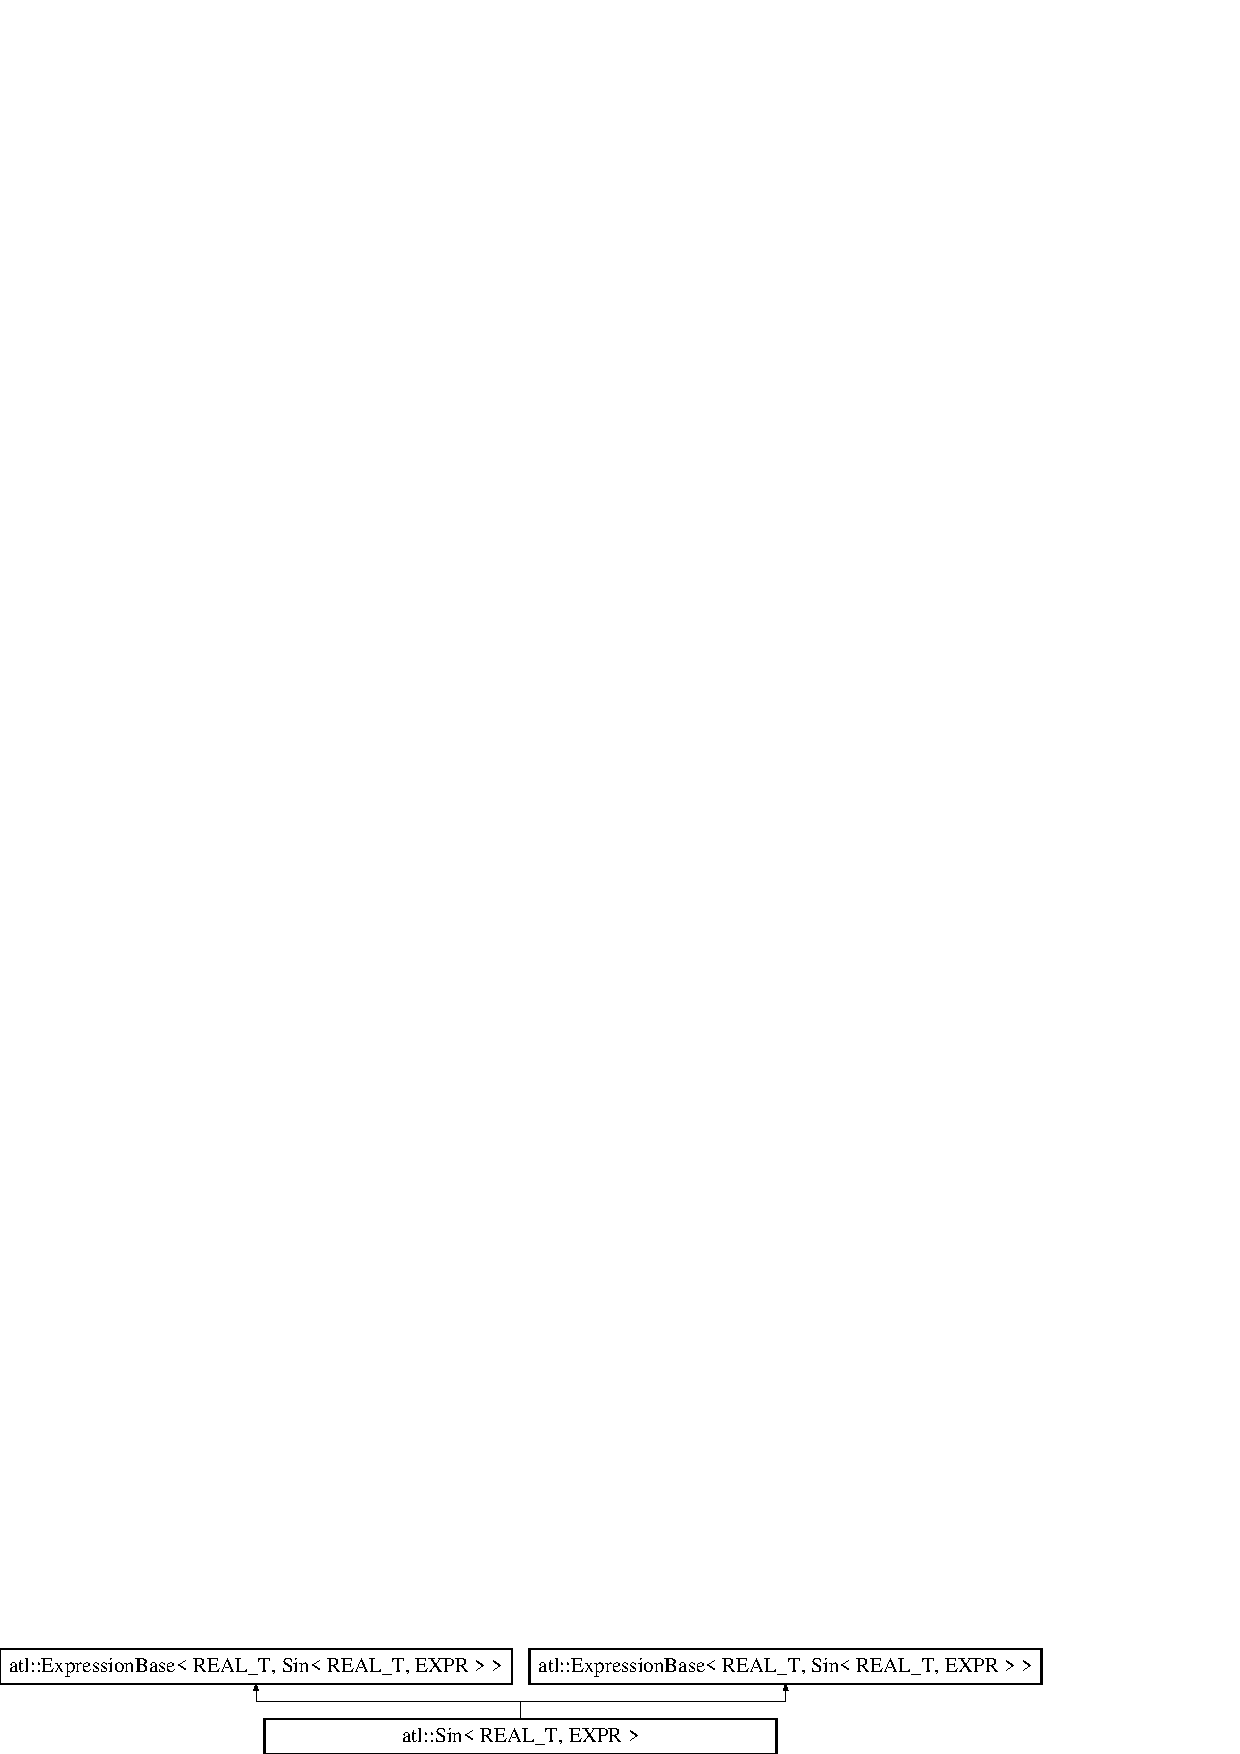
\includegraphics[height=1.656805cm]{structatl_1_1_sin}
\end{center}
\end{figure}
\subsection*{Public Types}
\begin{DoxyCompactItemize}
\item 
\hypertarget{structatl_1_1_sin_a4d1a2c2f3e07204d313f386dd2133778}{typedef R\+E\+A\+L\+\_\+\+T {\bfseries B\+A\+S\+E\+\_\+\+T\+Y\+P\+E}}\label{structatl_1_1_sin_a4d1a2c2f3e07204d313f386dd2133778}

\item 
\hypertarget{structatl_1_1_sin_a4d1a2c2f3e07204d313f386dd2133778}{typedef R\+E\+A\+L\+\_\+\+T {\bfseries B\+A\+S\+E\+\_\+\+T\+Y\+P\+E}}\label{structatl_1_1_sin_a4d1a2c2f3e07204d313f386dd2133778}

\end{DoxyCompactItemize}
\subsection*{Public Member Functions}
\begin{DoxyCompactItemize}
\item 
\hypertarget{structatl_1_1_sin_a3df17d8ff481eb5f7f28124f4679f57a}{{\bfseries Sin} (const \hyperlink{structatl_1_1_expression_base}{Expression\+Base}$<$ R\+E\+A\+L\+\_\+\+T, E\+X\+P\+R $>$ \&a)}\label{structatl_1_1_sin_a3df17d8ff481eb5f7f28124f4679f57a}

\item 
\hypertarget{structatl_1_1_sin_a33dcd22967cf5fcbfc6b4ee03ba577da}{const R\+E\+A\+L\+\_\+\+T {\bfseries Get\+Value} () const }\label{structatl_1_1_sin_a33dcd22967cf5fcbfc6b4ee03ba577da}

\item 
\hypertarget{structatl_1_1_sin_aaed0fa6931d8bbdcf99a9fd90ad39762}{const R\+E\+A\+L\+\_\+\+T {\bfseries Get\+Value} (size\+\_\+t i, size\+\_\+t j=0) const }\label{structatl_1_1_sin_aaed0fa6931d8bbdcf99a9fd90ad39762}

\item 
\hypertarget{structatl_1_1_sin_aa56f96071ecd7ca0deb76bfec206121a}{void {\bfseries Push\+Ids} (typename \hyperlink{structatl_1_1_stack_entry}{atl\+::\+Stack\+Entry}$<$ R\+E\+A\+L\+\_\+\+T $>$\+::vi\+\_\+storage \&ids) const }\label{structatl_1_1_sin_aa56f96071ecd7ca0deb76bfec206121a}

\item 
\hypertarget{structatl_1_1_sin_ae8a1e5a0999a8482c13e94aada70ffa8}{void {\bfseries Push\+Ids} (typename \hyperlink{structatl_1_1_stack_entry}{atl\+::\+Stack\+Entry}$<$ R\+E\+A\+L\+\_\+\+T $>$\+::vi\+\_\+storage \&ids, size\+\_\+t i, size\+\_\+t j=0) const }\label{structatl_1_1_sin_ae8a1e5a0999a8482c13e94aada70ffa8}

\item 
\hypertarget{structatl_1_1_sin_acd21686f4f342cb039451d2b2cb679c7}{const R\+E\+A\+L\+\_\+\+T {\bfseries Evaluate\+Derivative} (uint32\+\_\+t id) const }\label{structatl_1_1_sin_acd21686f4f342cb039451d2b2cb679c7}

\item 
\hypertarget{structatl_1_1_sin_aa04776c66ce58b543fcdc2ce0c2e5d00}{R\+E\+A\+L\+\_\+\+T {\bfseries Evaluate\+Derivative} (uint32\+\_\+t a, uint32\+\_\+t b) const }\label{structatl_1_1_sin_aa04776c66ce58b543fcdc2ce0c2e5d00}

\item 
\hypertarget{structatl_1_1_sin_ac050a241fa8fab93a53c51c036472554}{R\+E\+A\+L\+\_\+\+T {\bfseries Evaluate\+Derivative} (uint32\+\_\+t x, uint32\+\_\+t y, uint32\+\_\+t z) const }\label{structatl_1_1_sin_ac050a241fa8fab93a53c51c036472554}

\item 
\hypertarget{structatl_1_1_sin_a4ef555e663d120f338a3bad7005cecc9}{const R\+E\+A\+L\+\_\+\+T {\bfseries Evaluate\+Derivative} (uint32\+\_\+t id, size\+\_\+t i, size\+\_\+t j=0) const }\label{structatl_1_1_sin_a4ef555e663d120f338a3bad7005cecc9}

\item 
\hypertarget{structatl_1_1_sin_af4ef53a8b26e3790f66e07427c13cb72}{R\+E\+A\+L\+\_\+\+T {\bfseries Evaluate\+Derivative} (uint32\+\_\+t a, uint32\+\_\+t b, size\+\_\+t i, size\+\_\+t j=0) const }\label{structatl_1_1_sin_af4ef53a8b26e3790f66e07427c13cb72}

\item 
\hypertarget{structatl_1_1_sin_adee924b42b7927a6ba8e272735c79a65}{R\+E\+A\+L\+\_\+\+T {\bfseries Evaluate\+Derivative} (uint32\+\_\+t x, uint32\+\_\+t y, uint32\+\_\+t z, size\+\_\+t i, size\+\_\+t j=0) const }\label{structatl_1_1_sin_adee924b42b7927a6ba8e272735c79a65}

\item 
\hypertarget{structatl_1_1_sin_ad2272963bacc4ddf1c9507967b0405f8}{size\+\_\+t {\bfseries Get\+Columns} () const }\label{structatl_1_1_sin_ad2272963bacc4ddf1c9507967b0405f8}

\item 
\hypertarget{structatl_1_1_sin_a7e4fc8f849125a5e048772b1849655e1}{size\+\_\+t {\bfseries Get\+Rows} () const }\label{structatl_1_1_sin_a7e4fc8f849125a5e048772b1849655e1}

\item 
\hypertarget{structatl_1_1_sin_a7d9afdaaefe56e146b96a4945ff2bcbe}{bool {\bfseries Is\+Scalar} () const }\label{structatl_1_1_sin_a7d9afdaaefe56e146b96a4945ff2bcbe}

\item 
\hyperlink{structatl_1_1_sin_a3df17d8ff481eb5f7f28124f4679f57a}{Sin} (const \hyperlink{structatl_1_1_expression_base}{Expression\+Base}$<$ R\+E\+A\+L\+\_\+\+T, E\+X\+P\+R $>$ \&a)
\item 
const R\+E\+A\+L\+\_\+\+T \hyperlink{structatl_1_1_sin_a33dcd22967cf5fcbfc6b4ee03ba577da}{Get\+Value} () const 
\item 
const R\+E\+A\+L\+\_\+\+T \hyperlink{structatl_1_1_sin_aaed0fa6931d8bbdcf99a9fd90ad39762}{Get\+Value} (size\+\_\+t i, size\+\_\+t j=0) const 
\item 
bool \hyperlink{structatl_1_1_sin_a4b25a7cddd6215a986983f350bbe1c78}{Is\+Nonlinear} () const 
\item 
void \hyperlink{structatl_1_1_sin_aa56f96071ecd7ca0deb76bfec206121a}{Push\+Ids} (typename \hyperlink{structatl_1_1_stack_entry}{atl\+::\+Stack\+Entry}$<$ R\+E\+A\+L\+\_\+\+T $>$\+::vi\+\_\+storage \&ids) const 
\item 
void \hyperlink{structatl_1_1_sin_ae8a1e5a0999a8482c13e94aada70ffa8}{Push\+Ids} (typename \hyperlink{structatl_1_1_stack_entry}{atl\+::\+Stack\+Entry}$<$ R\+E\+A\+L\+\_\+\+T $>$\+::vi\+\_\+storage \&ids, size\+\_\+t i, size\+\_\+t j=0) const 
\item 
const R\+E\+A\+L\+\_\+\+T \hyperlink{structatl_1_1_sin_a45ce01d1f6f20dc03a8bcc38ace4bbfd}{Evaluate\+Derivative} (uint32\+\_\+t x) const 
\item 
R\+E\+A\+L\+\_\+\+T \hyperlink{structatl_1_1_sin_a5c0eb6f6ed68d7d204acfac19ddb89b7}{Evaluate\+Derivative} (uint32\+\_\+t x, uint32\+\_\+t y) const 
\item 
R\+E\+A\+L\+\_\+\+T \hyperlink{structatl_1_1_sin_ac050a241fa8fab93a53c51c036472554}{Evaluate\+Derivative} (uint32\+\_\+t x, uint32\+\_\+t y, uint32\+\_\+t z) const 
\item 
const R\+E\+A\+L\+\_\+\+T \hyperlink{structatl_1_1_sin_aff3bd97670bbc85fbde6fc0ae230f848}{Evaluate\+Derivative} (uint32\+\_\+t x, size\+\_\+t i, size\+\_\+t j=0) const 
\item 
R\+E\+A\+L\+\_\+\+T \hyperlink{structatl_1_1_sin_ac2df0e957a446956538a99e625371063}{Evaluate\+Derivative} (uint32\+\_\+t x, uint32\+\_\+t y, size\+\_\+t i, size\+\_\+t j=0) const 
\item 
R\+E\+A\+L\+\_\+\+T \hyperlink{structatl_1_1_sin_adee924b42b7927a6ba8e272735c79a65}{Evaluate\+Derivative} (uint32\+\_\+t x, uint32\+\_\+t y, uint32\+\_\+t z, size\+\_\+t i, size\+\_\+t j=0) const 
\item 
size\+\_\+t \hyperlink{structatl_1_1_sin_a7e4fc8f849125a5e048772b1849655e1}{Get\+Rows} () const 
\item 
bool \hyperlink{structatl_1_1_sin_a7d9afdaaefe56e146b96a4945ff2bcbe}{Is\+Scalar} () const 
\item 
const std\+::string \hyperlink{structatl_1_1_sin_ae9305f44533e915d6d7a9e24aa6d6fd5}{To\+Expression\+Template\+String} () const 
\end{DoxyCompactItemize}
\subsection*{Public Attributes}
\begin{DoxyCompactItemize}
\item 
\hypertarget{structatl_1_1_sin_a1362a397085201ac907aa683a90ddc63}{const E\+X\+P\+R \& {\bfseries expr\+\_\+m}}\label{structatl_1_1_sin_a1362a397085201ac907aa683a90ddc63}

\end{DoxyCompactItemize}


\subsection{Detailed Description}
\subsubsection*{template$<$class R\+E\+A\+L\+\_\+\+T, class E\+X\+P\+R$>$struct atl\+::\+Sin$<$ R\+E\+A\+L\+\_\+\+T, E\+X\+P\+R $>$}

Expression template to handle sine for variable or container expressions.

$ \sin f(x) $

or

$ \sin f_{i,j}(x) $ 

\subsection{Constructor \& Destructor Documentation}
\hypertarget{structatl_1_1_sin_a3df17d8ff481eb5f7f28124f4679f57a}{\index{atl\+::\+Sin@{atl\+::\+Sin}!Sin@{Sin}}
\index{Sin@{Sin}!atl\+::\+Sin@{atl\+::\+Sin}}
\subsubsection[{Sin}]{\setlength{\rightskip}{0pt plus 5cm}template$<$class R\+E\+A\+L\+\_\+\+T , class E\+X\+P\+R $>$ {\bf atl\+::\+Sin}$<$ R\+E\+A\+L\+\_\+\+T, E\+X\+P\+R $>$\+::{\bf Sin} (
\begin{DoxyParamCaption}
\item[{const {\bf Expression\+Base}$<$ R\+E\+A\+L\+\_\+\+T, E\+X\+P\+R $>$ \&}]{a}
\end{DoxyParamCaption}
)\hspace{0.3cm}{\ttfamily [inline]}}}\label{structatl_1_1_sin_a3df17d8ff481eb5f7f28124f4679f57a}
Constructor


\begin{DoxyParams}{Parameters}
{\em a} & \\
\hline
\end{DoxyParams}


\subsection{Member Function Documentation}
\hypertarget{structatl_1_1_sin_a45ce01d1f6f20dc03a8bcc38ace4bbfd}{\index{atl\+::\+Sin@{atl\+::\+Sin}!Evaluate\+Derivative@{Evaluate\+Derivative}}
\index{Evaluate\+Derivative@{Evaluate\+Derivative}!atl\+::\+Sin@{atl\+::\+Sin}}
\subsubsection[{Evaluate\+Derivative}]{\setlength{\rightskip}{0pt plus 5cm}template$<$class R\+E\+A\+L\+\_\+\+T , class E\+X\+P\+R $>$ const R\+E\+A\+L\+\_\+\+T {\bf atl\+::\+Sin}$<$ R\+E\+A\+L\+\_\+\+T, E\+X\+P\+R $>$\+::Evaluate\+Derivative (
\begin{DoxyParamCaption}
\item[{uint32\+\_\+t}]{x}
\end{DoxyParamCaption}
) const\hspace{0.3cm}{\ttfamily [inline]}}}\label{structatl_1_1_sin_a45ce01d1f6f20dc03a8bcc38ace4bbfd}
Evaluates the first-\/order derivative with respect to x.

$ \cos f(x)\,\left({{d}\over{d\,x}}\,f(x)\right) $


\begin{DoxyParams}{Parameters}
{\em x} & \\
\hline
\end{DoxyParams}
\begin{DoxyReturn}{Returns}

\end{DoxyReturn}
\hypertarget{structatl_1_1_sin_a5c0eb6f6ed68d7d204acfac19ddb89b7}{\index{atl\+::\+Sin@{atl\+::\+Sin}!Evaluate\+Derivative@{Evaluate\+Derivative}}
\index{Evaluate\+Derivative@{Evaluate\+Derivative}!atl\+::\+Sin@{atl\+::\+Sin}}
\subsubsection[{Evaluate\+Derivative}]{\setlength{\rightskip}{0pt plus 5cm}template$<$class R\+E\+A\+L\+\_\+\+T , class E\+X\+P\+R $>$ R\+E\+A\+L\+\_\+\+T {\bf atl\+::\+Sin}$<$ R\+E\+A\+L\+\_\+\+T, E\+X\+P\+R $>$\+::Evaluate\+Derivative (
\begin{DoxyParamCaption}
\item[{uint32\+\_\+t}]{x, }
\item[{uint32\+\_\+t}]{y}
\end{DoxyParamCaption}
) const\hspace{0.3cm}{\ttfamily [inline]}}}\label{structatl_1_1_sin_a5c0eb6f6ed68d7d204acfac19ddb89b7}
Evaluates the second-\/order derivative with respect to x and y.

$ \cos f(x,y)\,\left({{d^2}\over{d\,x\,d\,y}}\,f(x,y) \right)-\sin f(x,y)\,\left({{d}\over{d\,x}}\,f(x,y) \right)\,\left({{d}\over{d\,y}}\,f(x,y)\right) $


\begin{DoxyParams}{Parameters}
{\em x} & \\
\hline
{\em y} & \\
\hline
\end{DoxyParams}
\begin{DoxyReturn}{Returns}

\end{DoxyReturn}
\hypertarget{structatl_1_1_sin_ac050a241fa8fab93a53c51c036472554}{\index{atl\+::\+Sin@{atl\+::\+Sin}!Evaluate\+Derivative@{Evaluate\+Derivative}}
\index{Evaluate\+Derivative@{Evaluate\+Derivative}!atl\+::\+Sin@{atl\+::\+Sin}}
\subsubsection[{Evaluate\+Derivative}]{\setlength{\rightskip}{0pt plus 5cm}template$<$class R\+E\+A\+L\+\_\+\+T , class E\+X\+P\+R $>$ R\+E\+A\+L\+\_\+\+T {\bf atl\+::\+Sin}$<$ R\+E\+A\+L\+\_\+\+T, E\+X\+P\+R $>$\+::Evaluate\+Derivative (
\begin{DoxyParamCaption}
\item[{uint32\+\_\+t}]{x, }
\item[{uint32\+\_\+t}]{y, }
\item[{uint32\+\_\+t}]{z}
\end{DoxyParamCaption}
) const\hspace{0.3cm}{\ttfamily [inline]}}}\label{structatl_1_1_sin_ac050a241fa8fab93a53c51c036472554}
Evaluates the third-\/order derivative with respect to x, y, and z..

$ -\cos f(x,y,z)\,\left({{d}\over{d\,x}}\,f(x,y,z)\right) \,\left({{d}\over{d\,y}}\,f(x,y,z)\right)\,\left({{d}\over{d\, z}}\,f(x,y,z)\right)-\sin f(x,y,z)\,\left({{d^2}\over{d \,x\,d\,y}}\,f(x,y,z)\right)\,\left({{d}\over{d\,z}}\,f( x,y,z)\right)- \\ \sin f(x,y,z)\,\left({{d}\over{d\,x}}\,f(x ,y,z)\right)\,\left({{d^2}\over{d\,y\,d\,z}}\,f(x,y,z)\right)- \sin f(x,y,z)\,\left({{d^2}\over{d\,x\,d\,z}}\,f(x,y,z) \right)\,\left({{d}\over{d\,y}}\,f(x,y,z)\right)+\cos f( x,y,z)\,\left({{d^3}\over{d\,x\,d\,y\,d\,z}}\,f(x,y,z)\right) $


\begin{DoxyParams}{Parameters}
{\em x} & \\
\hline
{\em y} & \\
\hline
{\em z} & \\
\hline
\end{DoxyParams}
\begin{DoxyReturn}{Returns}

\end{DoxyReturn}
\hypertarget{structatl_1_1_sin_aff3bd97670bbc85fbde6fc0ae230f848}{\index{atl\+::\+Sin@{atl\+::\+Sin}!Evaluate\+Derivative@{Evaluate\+Derivative}}
\index{Evaluate\+Derivative@{Evaluate\+Derivative}!atl\+::\+Sin@{atl\+::\+Sin}}
\subsubsection[{Evaluate\+Derivative}]{\setlength{\rightskip}{0pt plus 5cm}template$<$class R\+E\+A\+L\+\_\+\+T , class E\+X\+P\+R $>$ const R\+E\+A\+L\+\_\+\+T {\bf atl\+::\+Sin}$<$ R\+E\+A\+L\+\_\+\+T, E\+X\+P\+R $>$\+::Evaluate\+Derivative (
\begin{DoxyParamCaption}
\item[{uint32\+\_\+t}]{x, }
\item[{size\+\_\+t}]{i, }
\item[{size\+\_\+t}]{j = {\ttfamily 0}}
\end{DoxyParamCaption}
) const\hspace{0.3cm}{\ttfamily [inline]}}}\label{structatl_1_1_sin_aff3bd97670bbc85fbde6fc0ae230f848}
Evaluates the first-\/order derivative with respect to x at index \{i,j\}.

$ \cos f_{i,j}(x)\,\left({{d}\over{d\,x}}\,f_{i,j}(x)\right) $


\begin{DoxyParams}{Parameters}
{\em x} & \\
\hline
\end{DoxyParams}
\begin{DoxyReturn}{Returns}

\end{DoxyReturn}
\hypertarget{structatl_1_1_sin_ac2df0e957a446956538a99e625371063}{\index{atl\+::\+Sin@{atl\+::\+Sin}!Evaluate\+Derivative@{Evaluate\+Derivative}}
\index{Evaluate\+Derivative@{Evaluate\+Derivative}!atl\+::\+Sin@{atl\+::\+Sin}}
\subsubsection[{Evaluate\+Derivative}]{\setlength{\rightskip}{0pt plus 5cm}template$<$class R\+E\+A\+L\+\_\+\+T , class E\+X\+P\+R $>$ R\+E\+A\+L\+\_\+\+T {\bf atl\+::\+Sin}$<$ R\+E\+A\+L\+\_\+\+T, E\+X\+P\+R $>$\+::Evaluate\+Derivative (
\begin{DoxyParamCaption}
\item[{uint32\+\_\+t}]{x, }
\item[{uint32\+\_\+t}]{y, }
\item[{size\+\_\+t}]{i, }
\item[{size\+\_\+t}]{j = {\ttfamily 0}}
\end{DoxyParamCaption}
) const\hspace{0.3cm}{\ttfamily [inline]}}}\label{structatl_1_1_sin_ac2df0e957a446956538a99e625371063}
Evaluates the second-\/order derivative with respect to x and y at index \{i,j\}.

$ \cos f_{i,j}(x,y)\,\left({{d^2}\over{d\,x\,d\,y}}\,f_{i,j}(x,y) \right)-\sin f_{i,j}(x,y)\,\left({{d}\over{d\,x}}\,f_{i,j}(x,y) \right)\,\left({{d}\over{d\,y}}\,f_{i,j}(x,y)\right) $


\begin{DoxyParams}{Parameters}
{\em x} & \\
\hline
{\em y} & \\
\hline
\end{DoxyParams}
\begin{DoxyReturn}{Returns}

\end{DoxyReturn}
\hypertarget{structatl_1_1_sin_adee924b42b7927a6ba8e272735c79a65}{\index{atl\+::\+Sin@{atl\+::\+Sin}!Evaluate\+Derivative@{Evaluate\+Derivative}}
\index{Evaluate\+Derivative@{Evaluate\+Derivative}!atl\+::\+Sin@{atl\+::\+Sin}}
\subsubsection[{Evaluate\+Derivative}]{\setlength{\rightskip}{0pt plus 5cm}template$<$class R\+E\+A\+L\+\_\+\+T , class E\+X\+P\+R $>$ R\+E\+A\+L\+\_\+\+T {\bf atl\+::\+Sin}$<$ R\+E\+A\+L\+\_\+\+T, E\+X\+P\+R $>$\+::Evaluate\+Derivative (
\begin{DoxyParamCaption}
\item[{uint32\+\_\+t}]{x, }
\item[{uint32\+\_\+t}]{y, }
\item[{uint32\+\_\+t}]{z, }
\item[{size\+\_\+t}]{i, }
\item[{size\+\_\+t}]{j = {\ttfamily 0}}
\end{DoxyParamCaption}
) const\hspace{0.3cm}{\ttfamily [inline]}}}\label{structatl_1_1_sin_adee924b42b7927a6ba8e272735c79a65}
Evaluates the third-\/order derivative with respect to x, y, and z at index \{i,j\}.

$ -\cos f_{i,j}(x,y,z)\,\left({{d}\over{d\,x}}\,f_{i,j}(x,y,z)\right) \,\left({{d}\over{d\,y}}\,f_{i,j}(x,y,z)\right)\,\left({{d}\over{d\, z}}\,f_{i,j}(x,y,z)\right)-\sin f_{i,j}(x,y,z)\,\left({{d^2}\over{d \,x\,d\,y}}\,f_{i,j}(x,y,z)\right)\,\left({{d}\over{d\,z}}\,f_{i,j}( x,y,z)\right)- \\ \sin f_{i,j}(x,y,z)\,\left({{d}\over{d\,x}}\,f_{i,j}(x ,y,z)\right)\,\left({{d^2}\over{d\,y\,d\,z}}\,f_{i,j}(x,y,z)\right)- \sin f_{i,j}(x,y,z)\,\left({{d^2}\over{d\,x\,d\,z}}\,f_{i,j}(x,y,z) \right)\,\left({{d}\over{d\,y}}\,f_{i,j}(x,y,z)\right)+\cos f_{i,j}( x,y,z)\,\left({{d^3}\over{d\,x\,d\,y\,d\,z}}\,f_{i,j}(x,y,z)\right) $


\begin{DoxyParams}{Parameters}
{\em x} & \\
\hline
{\em y} & \\
\hline
{\em z} & \\
\hline
{\em i} & \\
\hline
{\em j} & \\
\hline
\end{DoxyParams}
\begin{DoxyReturn}{Returns}

\end{DoxyReturn}
\hypertarget{structatl_1_1_sin_a7e4fc8f849125a5e048772b1849655e1}{\index{atl\+::\+Sin@{atl\+::\+Sin}!Get\+Rows@{Get\+Rows}}
\index{Get\+Rows@{Get\+Rows}!atl\+::\+Sin@{atl\+::\+Sin}}
\subsubsection[{Get\+Rows}]{\setlength{\rightskip}{0pt plus 5cm}template$<$class R\+E\+A\+L\+\_\+\+T , class E\+X\+P\+R $>$ size\+\_\+t {\bf atl\+::\+Sin}$<$ R\+E\+A\+L\+\_\+\+T, E\+X\+P\+R $>$\+::Get\+Rows (
\begin{DoxyParamCaption}
{}
\end{DoxyParamCaption}
) const\hspace{0.3cm}{\ttfamily [inline]}}}\label{structatl_1_1_sin_a7e4fc8f849125a5e048772b1849655e1}
Return the number of rows.

\begin{DoxyReturn}{Returns}

\end{DoxyReturn}
\hypertarget{structatl_1_1_sin_a33dcd22967cf5fcbfc6b4ee03ba577da}{\index{atl\+::\+Sin@{atl\+::\+Sin}!Get\+Value@{Get\+Value}}
\index{Get\+Value@{Get\+Value}!atl\+::\+Sin@{atl\+::\+Sin}}
\subsubsection[{Get\+Value}]{\setlength{\rightskip}{0pt plus 5cm}template$<$class R\+E\+A\+L\+\_\+\+T , class E\+X\+P\+R $>$ const R\+E\+A\+L\+\_\+\+T {\bf atl\+::\+Sin}$<$ R\+E\+A\+L\+\_\+\+T, E\+X\+P\+R $>$\+::Get\+Value (
\begin{DoxyParamCaption}
{}
\end{DoxyParamCaption}
) const\hspace{0.3cm}{\ttfamily [inline]}}}\label{structatl_1_1_sin_a33dcd22967cf5fcbfc6b4ee03ba577da}
Compute the sine of the evaluated expression.

\begin{DoxyReturn}{Returns}

\end{DoxyReturn}
\hypertarget{structatl_1_1_sin_aaed0fa6931d8bbdcf99a9fd90ad39762}{\index{atl\+::\+Sin@{atl\+::\+Sin}!Get\+Value@{Get\+Value}}
\index{Get\+Value@{Get\+Value}!atl\+::\+Sin@{atl\+::\+Sin}}
\subsubsection[{Get\+Value}]{\setlength{\rightskip}{0pt plus 5cm}template$<$class R\+E\+A\+L\+\_\+\+T , class E\+X\+P\+R $>$ const R\+E\+A\+L\+\_\+\+T {\bf atl\+::\+Sin}$<$ R\+E\+A\+L\+\_\+\+T, E\+X\+P\+R $>$\+::Get\+Value (
\begin{DoxyParamCaption}
\item[{size\+\_\+t}]{i, }
\item[{size\+\_\+t}]{j = {\ttfamily 0}}
\end{DoxyParamCaption}
) const\hspace{0.3cm}{\ttfamily [inline]}}}\label{structatl_1_1_sin_aaed0fa6931d8bbdcf99a9fd90ad39762}
Compute the sine of the evaluated expression at index \{i,j\}.

\begin{DoxyReturn}{Returns}

\end{DoxyReturn}
\hypertarget{structatl_1_1_sin_a4b25a7cddd6215a986983f350bbe1c78}{\index{atl\+::\+Sin@{atl\+::\+Sin}!Is\+Nonlinear@{Is\+Nonlinear}}
\index{Is\+Nonlinear@{Is\+Nonlinear}!atl\+::\+Sin@{atl\+::\+Sin}}
\subsubsection[{Is\+Nonlinear}]{\setlength{\rightskip}{0pt plus 5cm}template$<$class R\+E\+A\+L\+\_\+\+T , class E\+X\+P\+R $>$ bool {\bf atl\+::\+Sin}$<$ R\+E\+A\+L\+\_\+\+T, E\+X\+P\+R $>$\+::Is\+Nonlinear (
\begin{DoxyParamCaption}
{}
\end{DoxyParamCaption}
) const\hspace{0.3cm}{\ttfamily [inline]}}}\label{structatl_1_1_sin_a4b25a7cddd6215a986983f350bbe1c78}
Returns true.

\begin{DoxyReturn}{Returns}

\end{DoxyReturn}
\hypertarget{structatl_1_1_sin_a7d9afdaaefe56e146b96a4945ff2bcbe}{\index{atl\+::\+Sin@{atl\+::\+Sin}!Is\+Scalar@{Is\+Scalar}}
\index{Is\+Scalar@{Is\+Scalar}!atl\+::\+Sin@{atl\+::\+Sin}}
\subsubsection[{Is\+Scalar}]{\setlength{\rightskip}{0pt plus 5cm}template$<$class R\+E\+A\+L\+\_\+\+T , class E\+X\+P\+R $>$ bool {\bf atl\+::\+Sin}$<$ R\+E\+A\+L\+\_\+\+T, E\+X\+P\+R $>$\+::Is\+Scalar (
\begin{DoxyParamCaption}
{}
\end{DoxyParamCaption}
) const\hspace{0.3cm}{\ttfamily [inline]}}}\label{structatl_1_1_sin_a7d9afdaaefe56e146b96a4945ff2bcbe}
True if this expression is a scalar.

\begin{DoxyReturn}{Returns}

\end{DoxyReturn}
\hypertarget{structatl_1_1_sin_aa56f96071ecd7ca0deb76bfec206121a}{\index{atl\+::\+Sin@{atl\+::\+Sin}!Push\+Ids@{Push\+Ids}}
\index{Push\+Ids@{Push\+Ids}!atl\+::\+Sin@{atl\+::\+Sin}}
\subsubsection[{Push\+Ids}]{\setlength{\rightskip}{0pt plus 5cm}template$<$class R\+E\+A\+L\+\_\+\+T , class E\+X\+P\+R $>$ void {\bf atl\+::\+Sin}$<$ R\+E\+A\+L\+\_\+\+T, E\+X\+P\+R $>$\+::Push\+Ids (
\begin{DoxyParamCaption}
\item[{typename {\bf atl\+::\+Stack\+Entry}$<$ R\+E\+A\+L\+\_\+\+T $>$\+::vi\+\_\+storage \&}]{ids}
\end{DoxyParamCaption}
) const\hspace{0.3cm}{\ttfamily [inline]}}}\label{structatl_1_1_sin_aa56f96071ecd7ca0deb76bfec206121a}
Push variable info into a set.


\begin{DoxyParams}{Parameters}
{\em ids} & \\
\hline
\end{DoxyParams}
\hypertarget{structatl_1_1_sin_ae8a1e5a0999a8482c13e94aada70ffa8}{\index{atl\+::\+Sin@{atl\+::\+Sin}!Push\+Ids@{Push\+Ids}}
\index{Push\+Ids@{Push\+Ids}!atl\+::\+Sin@{atl\+::\+Sin}}
\subsubsection[{Push\+Ids}]{\setlength{\rightskip}{0pt plus 5cm}template$<$class R\+E\+A\+L\+\_\+\+T , class E\+X\+P\+R $>$ void {\bf atl\+::\+Sin}$<$ R\+E\+A\+L\+\_\+\+T, E\+X\+P\+R $>$\+::Push\+Ids (
\begin{DoxyParamCaption}
\item[{typename {\bf atl\+::\+Stack\+Entry}$<$ R\+E\+A\+L\+\_\+\+T $>$\+::vi\+\_\+storage \&}]{ids, }
\item[{size\+\_\+t}]{i, }
\item[{size\+\_\+t}]{j = {\ttfamily 0}}
\end{DoxyParamCaption}
) const\hspace{0.3cm}{\ttfamily [inline]}}}\label{structatl_1_1_sin_ae8a1e5a0999a8482c13e94aada70ffa8}
Push variable info into a set at index \{i,j\}.


\begin{DoxyParams}{Parameters}
{\em ids} & \\
\hline
{\em i} & \\
\hline
{\em j} & \\
\hline
\end{DoxyParams}
\hypertarget{structatl_1_1_sin_ae9305f44533e915d6d7a9e24aa6d6fd5}{\index{atl\+::\+Sin@{atl\+::\+Sin}!To\+Expression\+Template\+String@{To\+Expression\+Template\+String}}
\index{To\+Expression\+Template\+String@{To\+Expression\+Template\+String}!atl\+::\+Sin@{atl\+::\+Sin}}
\subsubsection[{To\+Expression\+Template\+String}]{\setlength{\rightskip}{0pt plus 5cm}template$<$class R\+E\+A\+L\+\_\+\+T , class E\+X\+P\+R $>$ const std\+::string {\bf atl\+::\+Sin}$<$ R\+E\+A\+L\+\_\+\+T, E\+X\+P\+R $>$\+::To\+Expression\+Template\+String (
\begin{DoxyParamCaption}
{}
\end{DoxyParamCaption}
) const\hspace{0.3cm}{\ttfamily [inline]}}}\label{structatl_1_1_sin_ae9305f44533e915d6d7a9e24aa6d6fd5}
Create a string representation of this expression template. \begin{DoxyReturn}{Returns}

\end{DoxyReturn}


The documentation for this struct was generated from the following file\+:\begin{DoxyCompactItemize}
\item 
A\+T\+L2/Sin.\+hpp\end{DoxyCompactItemize}

\hypertarget{structatl_1_1_sinh}{\section{atl\+:\+:Sinh$<$ R\+E\+A\+L\+\_\+\+T, E\+X\+P\+R $>$ Struct Template Reference}
\label{structatl_1_1_sinh}\index{atl\+::\+Sinh$<$ R\+E\+A\+L\+\_\+\+T, E\+X\+P\+R $>$@{atl\+::\+Sinh$<$ R\+E\+A\+L\+\_\+\+T, E\+X\+P\+R $>$}}
}


{\ttfamily \#include $<$Sinh.\+hpp$>$}

Inheritance diagram for atl\+:\+:Sinh$<$ R\+E\+A\+L\+\_\+\+T, E\+X\+P\+R $>$\+:\begin{figure}[H]
\begin{center}
\leavevmode
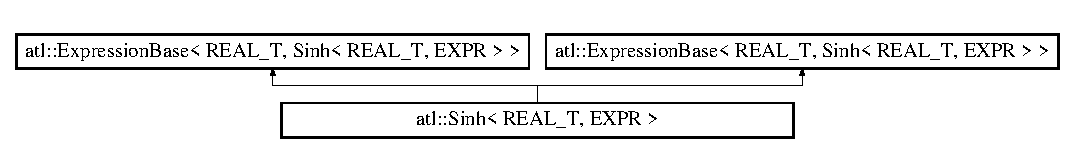
\includegraphics[height=1.623188cm]{structatl_1_1_sinh}
\end{center}
\end{figure}
\subsection*{Public Types}
\begin{DoxyCompactItemize}
\item 
\hypertarget{structatl_1_1_sinh_ab3df219c7affc407e843fb862c3eb909}{typedef R\+E\+A\+L\+\_\+\+T {\bfseries B\+A\+S\+E\+\_\+\+T\+Y\+P\+E}}\label{structatl_1_1_sinh_ab3df219c7affc407e843fb862c3eb909}

\item 
\hypertarget{structatl_1_1_sinh_ab3df219c7affc407e843fb862c3eb909}{typedef R\+E\+A\+L\+\_\+\+T {\bfseries B\+A\+S\+E\+\_\+\+T\+Y\+P\+E}}\label{structatl_1_1_sinh_ab3df219c7affc407e843fb862c3eb909}

\end{DoxyCompactItemize}
\subsection*{Public Member Functions}
\begin{DoxyCompactItemize}
\item 
\hypertarget{structatl_1_1_sinh_a384041506888c72dd5b68e81fa6b3943}{{\bfseries Sinh} (const \hyperlink{structatl_1_1_expression_base}{Expression\+Base}$<$ R\+E\+A\+L\+\_\+\+T, E\+X\+P\+R $>$ \&a)}\label{structatl_1_1_sinh_a384041506888c72dd5b68e81fa6b3943}

\item 
\hypertarget{structatl_1_1_sinh_aaf5066d39e86dae3dffa9abe77c9f924}{const R\+E\+A\+L\+\_\+\+T {\bfseries Get\+Value} () const }\label{structatl_1_1_sinh_aaf5066d39e86dae3dffa9abe77c9f924}

\item 
\hypertarget{structatl_1_1_sinh_a7589599a40e29cf02896222ea966e79f}{const R\+E\+A\+L\+\_\+\+T {\bfseries Get\+Value} (size\+\_\+t i, size\+\_\+t j=0) const }\label{structatl_1_1_sinh_a7589599a40e29cf02896222ea966e79f}

\item 
\hypertarget{structatl_1_1_sinh_a12d7cb5fef15afb217a023a5c6c2e05a}{void {\bfseries Push\+Ids} (typename \hyperlink{structatl_1_1_stack_entry}{atl\+::\+Stack\+Entry}$<$ R\+E\+A\+L\+\_\+\+T $>$\+::vi\+\_\+storage \&ids) const }\label{structatl_1_1_sinh_a12d7cb5fef15afb217a023a5c6c2e05a}

\item 
\hypertarget{structatl_1_1_sinh_ae5aaaa1b9a91fa00c9a1804ffd0348bb}{void {\bfseries Push\+Ids} (typename \hyperlink{structatl_1_1_stack_entry}{atl\+::\+Stack\+Entry}$<$ R\+E\+A\+L\+\_\+\+T $>$\+::vi\+\_\+storage \&ids, size\+\_\+t i, size\+\_\+t j=0) const }\label{structatl_1_1_sinh_ae5aaaa1b9a91fa00c9a1804ffd0348bb}

\item 
\hypertarget{structatl_1_1_sinh_ae15758db36d4cf71339418239d204b0e}{const R\+E\+A\+L\+\_\+\+T {\bfseries Evaluate\+Derivative} (uint32\+\_\+t id) const }\label{structatl_1_1_sinh_ae15758db36d4cf71339418239d204b0e}

\item 
\hypertarget{structatl_1_1_sinh_a2306a8e605b8f6a8a9913c97500719e9}{R\+E\+A\+L\+\_\+\+T {\bfseries Evaluate\+Derivative} (uint32\+\_\+t a, uint32\+\_\+t b) const }\label{structatl_1_1_sinh_a2306a8e605b8f6a8a9913c97500719e9}

\item 
\hypertarget{structatl_1_1_sinh_ae3a5b0a478d6ef9dcf8e1d20c8ed3f92}{R\+E\+A\+L\+\_\+\+T {\bfseries Evaluate\+Derivative} (uint32\+\_\+t x, uint32\+\_\+t y, uint32\+\_\+t z) const }\label{structatl_1_1_sinh_ae3a5b0a478d6ef9dcf8e1d20c8ed3f92}

\item 
\hypertarget{structatl_1_1_sinh_abc26f2f5ca270b6f30d00954a7e52fea}{const R\+E\+A\+L\+\_\+\+T {\bfseries Evaluate\+Derivative} (uint32\+\_\+t id, size\+\_\+t i, size\+\_\+t j=0) const }\label{structatl_1_1_sinh_abc26f2f5ca270b6f30d00954a7e52fea}

\item 
\hypertarget{structatl_1_1_sinh_afd606f2d72a12c124dcbc6550a16ab4f}{R\+E\+A\+L\+\_\+\+T {\bfseries Evaluate\+Derivative} (uint32\+\_\+t a, uint32\+\_\+t b, size\+\_\+t i, size\+\_\+t j=0) const }\label{structatl_1_1_sinh_afd606f2d72a12c124dcbc6550a16ab4f}

\item 
\hypertarget{structatl_1_1_sinh_a1ae010684050a6b765276e9807e57b8d}{R\+E\+A\+L\+\_\+\+T {\bfseries Evaluate\+Derivative} (uint32\+\_\+t x, uint32\+\_\+t y, uint32\+\_\+t z, size\+\_\+t i, size\+\_\+t j=0) const }\label{structatl_1_1_sinh_a1ae010684050a6b765276e9807e57b8d}

\item 
\hypertarget{structatl_1_1_sinh_ad3d34d429e780819850e02bc6acd8dc8}{size\+\_\+t {\bfseries Get\+Columns} () const }\label{structatl_1_1_sinh_ad3d34d429e780819850e02bc6acd8dc8}

\item 
\hypertarget{structatl_1_1_sinh_ad457a1e6c7544faa109bb7ce29b078aa}{size\+\_\+t {\bfseries Get\+Rows} () const }\label{structatl_1_1_sinh_ad457a1e6c7544faa109bb7ce29b078aa}

\item 
\hypertarget{structatl_1_1_sinh_aad6082b40f82274c6aebd2e2930246fc}{bool {\bfseries Is\+Scalar} () const }\label{structatl_1_1_sinh_aad6082b40f82274c6aebd2e2930246fc}

\item 
\hyperlink{structatl_1_1_sinh_a384041506888c72dd5b68e81fa6b3943}{Sinh} (const \hyperlink{structatl_1_1_expression_base}{Expression\+Base}$<$ R\+E\+A\+L\+\_\+\+T, E\+X\+P\+R $>$ \&a)
\item 
const R\+E\+A\+L\+\_\+\+T \hyperlink{structatl_1_1_sinh_aaf5066d39e86dae3dffa9abe77c9f924}{Get\+Value} () const 
\item 
const R\+E\+A\+L\+\_\+\+T \hyperlink{structatl_1_1_sinh_a7589599a40e29cf02896222ea966e79f}{Get\+Value} (size\+\_\+t i, size\+\_\+t j=0) const 
\item 
bool \hyperlink{structatl_1_1_sinh_a0cfcb839a00b3558cc1b87bb02eee3ef}{Is\+Nonlinear} () const 
\item 
void \hyperlink{structatl_1_1_sinh_a12d7cb5fef15afb217a023a5c6c2e05a}{Push\+Ids} (typename \hyperlink{structatl_1_1_stack_entry}{atl\+::\+Stack\+Entry}$<$ R\+E\+A\+L\+\_\+\+T $>$\+::vi\+\_\+storage \&ids) const 
\item 
void \hyperlink{structatl_1_1_sinh_ae5aaaa1b9a91fa00c9a1804ffd0348bb}{Push\+Ids} (typename \hyperlink{structatl_1_1_stack_entry}{atl\+::\+Stack\+Entry}$<$ R\+E\+A\+L\+\_\+\+T $>$\+::vi\+\_\+storage \&ids, size\+\_\+t i, size\+\_\+t j=0) const 
\item 
const R\+E\+A\+L\+\_\+\+T \hyperlink{structatl_1_1_sinh_a7d544f25b946a482a9f0c53632b426dc}{Evaluate\+Derivative} (uint32\+\_\+t x) const 
\item 
R\+E\+A\+L\+\_\+\+T \hyperlink{structatl_1_1_sinh_ac6feb969ec649a5bfdf4ac374df5c1f1}{Evaluate\+Derivative} (uint32\+\_\+t x, uint32\+\_\+t y) const 
\item 
R\+E\+A\+L\+\_\+\+T \hyperlink{structatl_1_1_sinh_ae3a5b0a478d6ef9dcf8e1d20c8ed3f92}{Evaluate\+Derivative} (uint32\+\_\+t x, uint32\+\_\+t y, uint32\+\_\+t z) const 
\item 
const R\+E\+A\+L\+\_\+\+T \hyperlink{structatl_1_1_sinh_a88d74f7ef8669a5679963189d1e00697}{Evaluate\+Derivative} (uint32\+\_\+t x, size\+\_\+t i, size\+\_\+t j=0) const 
\item 
R\+E\+A\+L\+\_\+\+T \hyperlink{structatl_1_1_sinh_ad77473e801567a8b4fa77fcd591818d8}{Evaluate\+Derivative} (uint32\+\_\+t x, uint32\+\_\+t y, size\+\_\+t i, size\+\_\+t j=0) const 
\item 
R\+E\+A\+L\+\_\+\+T \hyperlink{structatl_1_1_sinh_a1ae010684050a6b765276e9807e57b8d}{Evaluate\+Derivative} (uint32\+\_\+t x, uint32\+\_\+t y, uint32\+\_\+t z, size\+\_\+t i, size\+\_\+t j=0) const 
\item 
size\+\_\+t \hyperlink{structatl_1_1_sinh_ad457a1e6c7544faa109bb7ce29b078aa}{Get\+Rows} () const 
\item 
bool \hyperlink{structatl_1_1_sinh_aad6082b40f82274c6aebd2e2930246fc}{Is\+Scalar} () const 
\item 
const std\+::string \hyperlink{structatl_1_1_sinh_a772805639caf88e950b564523554292b}{To\+Expression\+Template\+String} () const 
\end{DoxyCompactItemize}
\subsection*{Public Attributes}
\begin{DoxyCompactItemize}
\item 
\hypertarget{structatl_1_1_sinh_a8752276cea6c6e79f0be4892d221afbc}{const E\+X\+P\+R \& {\bfseries expr\+\_\+m}}\label{structatl_1_1_sinh_a8752276cea6c6e79f0be4892d221afbc}

\end{DoxyCompactItemize}


\subsection{Detailed Description}
\subsubsection*{template$<$class R\+E\+A\+L\+\_\+\+T, class E\+X\+P\+R$>$struct atl\+::\+Sinh$<$ R\+E\+A\+L\+\_\+\+T, E\+X\+P\+R $>$}

Expression template to handle hyperbolic sine for variable or container expressions.

$ \sinh f(x) $

or

$ \sinh f_{i,j}(x) $ 

\subsection{Constructor \& Destructor Documentation}
\hypertarget{structatl_1_1_sinh_a384041506888c72dd5b68e81fa6b3943}{\index{atl\+::\+Sinh@{atl\+::\+Sinh}!Sinh@{Sinh}}
\index{Sinh@{Sinh}!atl\+::\+Sinh@{atl\+::\+Sinh}}
\subsubsection[{Sinh}]{\setlength{\rightskip}{0pt plus 5cm}template$<$class R\+E\+A\+L\+\_\+\+T , class E\+X\+P\+R $>$ {\bf atl\+::\+Sinh}$<$ R\+E\+A\+L\+\_\+\+T, E\+X\+P\+R $>$\+::{\bf Sinh} (
\begin{DoxyParamCaption}
\item[{const {\bf Expression\+Base}$<$ R\+E\+A\+L\+\_\+\+T, E\+X\+P\+R $>$ \&}]{a}
\end{DoxyParamCaption}
)\hspace{0.3cm}{\ttfamily [inline]}}}\label{structatl_1_1_sinh_a384041506888c72dd5b68e81fa6b3943}
Constructor


\begin{DoxyParams}{Parameters}
{\em a} & \\
\hline
\end{DoxyParams}


\subsection{Member Function Documentation}
\hypertarget{structatl_1_1_sinh_a7d544f25b946a482a9f0c53632b426dc}{\index{atl\+::\+Sinh@{atl\+::\+Sinh}!Evaluate\+Derivative@{Evaluate\+Derivative}}
\index{Evaluate\+Derivative@{Evaluate\+Derivative}!atl\+::\+Sinh@{atl\+::\+Sinh}}
\subsubsection[{Evaluate\+Derivative}]{\setlength{\rightskip}{0pt plus 5cm}template$<$class R\+E\+A\+L\+\_\+\+T , class E\+X\+P\+R $>$ const R\+E\+A\+L\+\_\+\+T {\bf atl\+::\+Sinh}$<$ R\+E\+A\+L\+\_\+\+T, E\+X\+P\+R $>$\+::Evaluate\+Derivative (
\begin{DoxyParamCaption}
\item[{uint32\+\_\+t}]{x}
\end{DoxyParamCaption}
) const\hspace{0.3cm}{\ttfamily [inline]}}}\label{structatl_1_1_sinh_a7d544f25b946a482a9f0c53632b426dc}
Evaluates the first-\/order derivative with respect to x.

$ \cosh f(x)\,\left({{d}\over{d\,x}}\,f(x)\right) $


\begin{DoxyParams}{Parameters}
{\em x} & \\
\hline
\end{DoxyParams}
\begin{DoxyReturn}{Returns}

\end{DoxyReturn}
\hypertarget{structatl_1_1_sinh_ac6feb969ec649a5bfdf4ac374df5c1f1}{\index{atl\+::\+Sinh@{atl\+::\+Sinh}!Evaluate\+Derivative@{Evaluate\+Derivative}}
\index{Evaluate\+Derivative@{Evaluate\+Derivative}!atl\+::\+Sinh@{atl\+::\+Sinh}}
\subsubsection[{Evaluate\+Derivative}]{\setlength{\rightskip}{0pt plus 5cm}template$<$class R\+E\+A\+L\+\_\+\+T , class E\+X\+P\+R $>$ R\+E\+A\+L\+\_\+\+T {\bf atl\+::\+Sinh}$<$ R\+E\+A\+L\+\_\+\+T, E\+X\+P\+R $>$\+::Evaluate\+Derivative (
\begin{DoxyParamCaption}
\item[{uint32\+\_\+t}]{x, }
\item[{uint32\+\_\+t}]{y}
\end{DoxyParamCaption}
) const\hspace{0.3cm}{\ttfamily [inline]}}}\label{structatl_1_1_sinh_ac6feb969ec649a5bfdf4ac374df5c1f1}
Evaluates the second-\/order derivative with respect to x and y at index \{i,j\}.

$ \sinh f(x,y)\,\left({{d}\over{d\,x}}\,f(x,y)\right)\, \left({{d}\over{d\,y}}\,f(x,y)\right)+\cosh f(x,y)\, \left({{d^2}\over{d\,x\,d\,y}}\,f(x,y)\right) $


\begin{DoxyParams}{Parameters}
{\em x} & \\
\hline
{\em y} & \\
\hline
\end{DoxyParams}
\begin{DoxyReturn}{Returns}

\end{DoxyReturn}
\hypertarget{structatl_1_1_sinh_ae3a5b0a478d6ef9dcf8e1d20c8ed3f92}{\index{atl\+::\+Sinh@{atl\+::\+Sinh}!Evaluate\+Derivative@{Evaluate\+Derivative}}
\index{Evaluate\+Derivative@{Evaluate\+Derivative}!atl\+::\+Sinh@{atl\+::\+Sinh}}
\subsubsection[{Evaluate\+Derivative}]{\setlength{\rightskip}{0pt plus 5cm}template$<$class R\+E\+A\+L\+\_\+\+T , class E\+X\+P\+R $>$ R\+E\+A\+L\+\_\+\+T {\bf atl\+::\+Sinh}$<$ R\+E\+A\+L\+\_\+\+T, E\+X\+P\+R $>$\+::Evaluate\+Derivative (
\begin{DoxyParamCaption}
\item[{uint32\+\_\+t}]{x, }
\item[{uint32\+\_\+t}]{y, }
\item[{uint32\+\_\+t}]{z}
\end{DoxyParamCaption}
) const\hspace{0.3cm}{\ttfamily [inline]}}}\label{structatl_1_1_sinh_ae3a5b0a478d6ef9dcf8e1d20c8ed3f92}
Evaluates the third-\/order derivative with respect to x, y, and z.

$ \cosh f(x,y,z)\,\left({{d}\over{d\,x}}\,f(x,y,z)\right) \,\left({{d}\over{d\,y}}\,f(x,y,z)\right)\,\left({{d}\over{d\, z}}\,f(x,y,z)\right)+\sinh f(x,y,z)\,\left({{d^2}\over{d \,x\,d\,y}}\,f(x,y,z)\right)\,\left({{d}\over{d\,z}}\,f( x,y,z)\right)+ \\ \sinh f(x,y,z)\,\left({{d}\over{d\,x}}\,f( x,y,z)\right)\,\left({{d^2}\over{d\,y\,d\,z}}\,f(x,y,z)\right) +\sinh f(x,y,z)\,\left({{d^2}\over{d\,x\,d\,z}}\,f(x,y,z )\right)\,\left({{d}\over{d\,y}}\,f(x,y,z)\right)+\cosh f_{i,j }(x,y,z)\,\left({{d^3}\over{d\,x\,d\,y\,d\,z}}\,f(x,y,z) \right) $


\begin{DoxyParams}{Parameters}
{\em x} & \\
\hline
{\em y} & \\
\hline
{\em z} & \\
\hline
\end{DoxyParams}
\begin{DoxyReturn}{Returns}

\end{DoxyReturn}
\hypertarget{structatl_1_1_sinh_a88d74f7ef8669a5679963189d1e00697}{\index{atl\+::\+Sinh@{atl\+::\+Sinh}!Evaluate\+Derivative@{Evaluate\+Derivative}}
\index{Evaluate\+Derivative@{Evaluate\+Derivative}!atl\+::\+Sinh@{atl\+::\+Sinh}}
\subsubsection[{Evaluate\+Derivative}]{\setlength{\rightskip}{0pt plus 5cm}template$<$class R\+E\+A\+L\+\_\+\+T , class E\+X\+P\+R $>$ const R\+E\+A\+L\+\_\+\+T {\bf atl\+::\+Sinh}$<$ R\+E\+A\+L\+\_\+\+T, E\+X\+P\+R $>$\+::Evaluate\+Derivative (
\begin{DoxyParamCaption}
\item[{uint32\+\_\+t}]{x, }
\item[{size\+\_\+t}]{i, }
\item[{size\+\_\+t}]{j = {\ttfamily 0}}
\end{DoxyParamCaption}
) const\hspace{0.3cm}{\ttfamily [inline]}}}\label{structatl_1_1_sinh_a88d74f7ef8669a5679963189d1e00697}
Evaluates the first-\/order derivative with respect to x at index \{i,j\}.

$ \cosh f_{i,j}(x)\,\left({{d}\over{d\,x}}\,f_{i,j}(x)\right) $


\begin{DoxyParams}{Parameters}
{\em x} & \\
\hline
{\em i} & \\
\hline
{\em j} & \\
\hline
\end{DoxyParams}
\begin{DoxyReturn}{Returns}

\end{DoxyReturn}
\hypertarget{structatl_1_1_sinh_ad77473e801567a8b4fa77fcd591818d8}{\index{atl\+::\+Sinh@{atl\+::\+Sinh}!Evaluate\+Derivative@{Evaluate\+Derivative}}
\index{Evaluate\+Derivative@{Evaluate\+Derivative}!atl\+::\+Sinh@{atl\+::\+Sinh}}
\subsubsection[{Evaluate\+Derivative}]{\setlength{\rightskip}{0pt plus 5cm}template$<$class R\+E\+A\+L\+\_\+\+T , class E\+X\+P\+R $>$ R\+E\+A\+L\+\_\+\+T {\bf atl\+::\+Sinh}$<$ R\+E\+A\+L\+\_\+\+T, E\+X\+P\+R $>$\+::Evaluate\+Derivative (
\begin{DoxyParamCaption}
\item[{uint32\+\_\+t}]{x, }
\item[{uint32\+\_\+t}]{y, }
\item[{size\+\_\+t}]{i, }
\item[{size\+\_\+t}]{j = {\ttfamily 0}}
\end{DoxyParamCaption}
) const\hspace{0.3cm}{\ttfamily [inline]}}}\label{structatl_1_1_sinh_ad77473e801567a8b4fa77fcd591818d8}
Evaluates the second-\/order derivative with respect to x and y at index \{i,j\}.

$ \sinh f_{i,j}(x,y)\,\left({{d}\over{d\,x}}\,f_{i,j}(x,y)\right)\, \left({{d}\over{d\,y}}\,f_{i,j}(x,y)\right)+\cosh f_{i,j}(x,y)\, \left({{d^2}\over{d\,x\,d\,y}}\,f_{i,j}(x,y)\right) $


\begin{DoxyParams}{Parameters}
{\em x} & \\
\hline
{\em y} & \\
\hline
{\em i} & \\
\hline
{\em j} & \\
\hline
\end{DoxyParams}
\begin{DoxyReturn}{Returns}

\end{DoxyReturn}
\hypertarget{structatl_1_1_sinh_a1ae010684050a6b765276e9807e57b8d}{\index{atl\+::\+Sinh@{atl\+::\+Sinh}!Evaluate\+Derivative@{Evaluate\+Derivative}}
\index{Evaluate\+Derivative@{Evaluate\+Derivative}!atl\+::\+Sinh@{atl\+::\+Sinh}}
\subsubsection[{Evaluate\+Derivative}]{\setlength{\rightskip}{0pt plus 5cm}template$<$class R\+E\+A\+L\+\_\+\+T , class E\+X\+P\+R $>$ R\+E\+A\+L\+\_\+\+T {\bf atl\+::\+Sinh}$<$ R\+E\+A\+L\+\_\+\+T, E\+X\+P\+R $>$\+::Evaluate\+Derivative (
\begin{DoxyParamCaption}
\item[{uint32\+\_\+t}]{x, }
\item[{uint32\+\_\+t}]{y, }
\item[{uint32\+\_\+t}]{z, }
\item[{size\+\_\+t}]{i, }
\item[{size\+\_\+t}]{j = {\ttfamily 0}}
\end{DoxyParamCaption}
) const\hspace{0.3cm}{\ttfamily [inline]}}}\label{structatl_1_1_sinh_a1ae010684050a6b765276e9807e57b8d}
Evaluates the third-\/order derivative with respect to x, y, and z at index \{i,j\}.

$ \cosh f_{i,j}(x,y,z)\,\left({{d}\over{d\,x}}\,f_{i,j}(x,y,z)\right) \,\left({{d}\over{d\,y}}\,f_{i,j}(x,y,z)\right)\,\left({{d}\over{d\, z}}\,f_{i,j}(x,y,z)\right)+\sinh f_{i,j}(x,y,z)\,\left({{d^2}\over{d \,x\,d\,y}}\,f_{i,j}(x,y,z)\right)\,\left({{d}\over{d\,z}}\,f_{i,j}( x,y,z)\right)+ \\ \sinh f_{i,j}(x,y,z)\,\left({{d}\over{d\,x}}\,f_{i,j}( x,y,z)\right)\,\left({{d^2}\over{d\,y\,d\,z}}\,f_{i,j}(x,y,z)\right) +\sinh f_{i,j}(x,y,z)\,\left({{d^2}\over{d\,x\,d\,z}}\,f_{i,j}(x,y,z )\right)\,\left({{d}\over{d\,y}}\,f_{i,j}(x,y,z)\right)+\cosh f_{i,j }(x,y,z)\,\left({{d^3}\over{d\,x\,d\,y\,d\,z}}\,f_{i,j}(x,y,z) \right) $


\begin{DoxyParams}{Parameters}
{\em x} & \\
\hline
{\em y} & \\
\hline
{\em z} & \\
\hline
{\em i} & \\
\hline
{\em j} & \\
\hline
\end{DoxyParams}
\begin{DoxyReturn}{Returns}

\end{DoxyReturn}
\hypertarget{structatl_1_1_sinh_ad457a1e6c7544faa109bb7ce29b078aa}{\index{atl\+::\+Sinh@{atl\+::\+Sinh}!Get\+Rows@{Get\+Rows}}
\index{Get\+Rows@{Get\+Rows}!atl\+::\+Sinh@{atl\+::\+Sinh}}
\subsubsection[{Get\+Rows}]{\setlength{\rightskip}{0pt plus 5cm}template$<$class R\+E\+A\+L\+\_\+\+T , class E\+X\+P\+R $>$ size\+\_\+t {\bf atl\+::\+Sinh}$<$ R\+E\+A\+L\+\_\+\+T, E\+X\+P\+R $>$\+::Get\+Rows (
\begin{DoxyParamCaption}
{}
\end{DoxyParamCaption}
) const\hspace{0.3cm}{\ttfamily [inline]}}}\label{structatl_1_1_sinh_ad457a1e6c7544faa109bb7ce29b078aa}
Return the number of rows.

\begin{DoxyReturn}{Returns}

\end{DoxyReturn}
\hypertarget{structatl_1_1_sinh_aaf5066d39e86dae3dffa9abe77c9f924}{\index{atl\+::\+Sinh@{atl\+::\+Sinh}!Get\+Value@{Get\+Value}}
\index{Get\+Value@{Get\+Value}!atl\+::\+Sinh@{atl\+::\+Sinh}}
\subsubsection[{Get\+Value}]{\setlength{\rightskip}{0pt plus 5cm}template$<$class R\+E\+A\+L\+\_\+\+T , class E\+X\+P\+R $>$ const R\+E\+A\+L\+\_\+\+T {\bf atl\+::\+Sinh}$<$ R\+E\+A\+L\+\_\+\+T, E\+X\+P\+R $>$\+::Get\+Value (
\begin{DoxyParamCaption}
{}
\end{DoxyParamCaption}
) const\hspace{0.3cm}{\ttfamily [inline]}}}\label{structatl_1_1_sinh_aaf5066d39e86dae3dffa9abe77c9f924}
Computes the hyperbolic sine of the evaluated expression.

\begin{DoxyReturn}{Returns}

\end{DoxyReturn}
\hypertarget{structatl_1_1_sinh_a7589599a40e29cf02896222ea966e79f}{\index{atl\+::\+Sinh@{atl\+::\+Sinh}!Get\+Value@{Get\+Value}}
\index{Get\+Value@{Get\+Value}!atl\+::\+Sinh@{atl\+::\+Sinh}}
\subsubsection[{Get\+Value}]{\setlength{\rightskip}{0pt plus 5cm}template$<$class R\+E\+A\+L\+\_\+\+T , class E\+X\+P\+R $>$ const R\+E\+A\+L\+\_\+\+T {\bf atl\+::\+Sinh}$<$ R\+E\+A\+L\+\_\+\+T, E\+X\+P\+R $>$\+::Get\+Value (
\begin{DoxyParamCaption}
\item[{size\+\_\+t}]{i, }
\item[{size\+\_\+t}]{j = {\ttfamily 0}}
\end{DoxyParamCaption}
) const\hspace{0.3cm}{\ttfamily [inline]}}}\label{structatl_1_1_sinh_a7589599a40e29cf02896222ea966e79f}
Computes the hyperbolic sine of the evaluated expression at index \{i,j\}.

\begin{DoxyReturn}{Returns}

\end{DoxyReturn}
\hypertarget{structatl_1_1_sinh_a0cfcb839a00b3558cc1b87bb02eee3ef}{\index{atl\+::\+Sinh@{atl\+::\+Sinh}!Is\+Nonlinear@{Is\+Nonlinear}}
\index{Is\+Nonlinear@{Is\+Nonlinear}!atl\+::\+Sinh@{atl\+::\+Sinh}}
\subsubsection[{Is\+Nonlinear}]{\setlength{\rightskip}{0pt plus 5cm}template$<$class R\+E\+A\+L\+\_\+\+T , class E\+X\+P\+R $>$ bool {\bf atl\+::\+Sinh}$<$ R\+E\+A\+L\+\_\+\+T, E\+X\+P\+R $>$\+::Is\+Nonlinear (
\begin{DoxyParamCaption}
{}
\end{DoxyParamCaption}
) const\hspace{0.3cm}{\ttfamily [inline]}}}\label{structatl_1_1_sinh_a0cfcb839a00b3558cc1b87bb02eee3ef}
Returns true.

\begin{DoxyReturn}{Returns}

\end{DoxyReturn}
\hypertarget{structatl_1_1_sinh_aad6082b40f82274c6aebd2e2930246fc}{\index{atl\+::\+Sinh@{atl\+::\+Sinh}!Is\+Scalar@{Is\+Scalar}}
\index{Is\+Scalar@{Is\+Scalar}!atl\+::\+Sinh@{atl\+::\+Sinh}}
\subsubsection[{Is\+Scalar}]{\setlength{\rightskip}{0pt plus 5cm}template$<$class R\+E\+A\+L\+\_\+\+T , class E\+X\+P\+R $>$ bool {\bf atl\+::\+Sinh}$<$ R\+E\+A\+L\+\_\+\+T, E\+X\+P\+R $>$\+::Is\+Scalar (
\begin{DoxyParamCaption}
{}
\end{DoxyParamCaption}
) const\hspace{0.3cm}{\ttfamily [inline]}}}\label{structatl_1_1_sinh_aad6082b40f82274c6aebd2e2930246fc}
True if this expression is a scalar.

\begin{DoxyReturn}{Returns}

\end{DoxyReturn}
\hypertarget{structatl_1_1_sinh_a12d7cb5fef15afb217a023a5c6c2e05a}{\index{atl\+::\+Sinh@{atl\+::\+Sinh}!Push\+Ids@{Push\+Ids}}
\index{Push\+Ids@{Push\+Ids}!atl\+::\+Sinh@{atl\+::\+Sinh}}
\subsubsection[{Push\+Ids}]{\setlength{\rightskip}{0pt plus 5cm}template$<$class R\+E\+A\+L\+\_\+\+T , class E\+X\+P\+R $>$ void {\bf atl\+::\+Sinh}$<$ R\+E\+A\+L\+\_\+\+T, E\+X\+P\+R $>$\+::Push\+Ids (
\begin{DoxyParamCaption}
\item[{typename {\bf atl\+::\+Stack\+Entry}$<$ R\+E\+A\+L\+\_\+\+T $>$\+::vi\+\_\+storage \&}]{ids}
\end{DoxyParamCaption}
) const\hspace{0.3cm}{\ttfamily [inline]}}}\label{structatl_1_1_sinh_a12d7cb5fef15afb217a023a5c6c2e05a}
Push variable info into a set.


\begin{DoxyParams}{Parameters}
{\em ids} & \\
\hline
\end{DoxyParams}
\hypertarget{structatl_1_1_sinh_ae5aaaa1b9a91fa00c9a1804ffd0348bb}{\index{atl\+::\+Sinh@{atl\+::\+Sinh}!Push\+Ids@{Push\+Ids}}
\index{Push\+Ids@{Push\+Ids}!atl\+::\+Sinh@{atl\+::\+Sinh}}
\subsubsection[{Push\+Ids}]{\setlength{\rightskip}{0pt plus 5cm}template$<$class R\+E\+A\+L\+\_\+\+T , class E\+X\+P\+R $>$ void {\bf atl\+::\+Sinh}$<$ R\+E\+A\+L\+\_\+\+T, E\+X\+P\+R $>$\+::Push\+Ids (
\begin{DoxyParamCaption}
\item[{typename {\bf atl\+::\+Stack\+Entry}$<$ R\+E\+A\+L\+\_\+\+T $>$\+::vi\+\_\+storage \&}]{ids, }
\item[{size\+\_\+t}]{i, }
\item[{size\+\_\+t}]{j = {\ttfamily 0}}
\end{DoxyParamCaption}
) const\hspace{0.3cm}{\ttfamily [inline]}}}\label{structatl_1_1_sinh_ae5aaaa1b9a91fa00c9a1804ffd0348bb}
Push variable info into a set at index \{i,j\}.


\begin{DoxyParams}{Parameters}
{\em ids} & \\
\hline
{\em i} & \\
\hline
{\em j} & \\
\hline
\end{DoxyParams}
\hypertarget{structatl_1_1_sinh_a772805639caf88e950b564523554292b}{\index{atl\+::\+Sinh@{atl\+::\+Sinh}!To\+Expression\+Template\+String@{To\+Expression\+Template\+String}}
\index{To\+Expression\+Template\+String@{To\+Expression\+Template\+String}!atl\+::\+Sinh@{atl\+::\+Sinh}}
\subsubsection[{To\+Expression\+Template\+String}]{\setlength{\rightskip}{0pt plus 5cm}template$<$class R\+E\+A\+L\+\_\+\+T , class E\+X\+P\+R $>$ const std\+::string {\bf atl\+::\+Sinh}$<$ R\+E\+A\+L\+\_\+\+T, E\+X\+P\+R $>$\+::To\+Expression\+Template\+String (
\begin{DoxyParamCaption}
{}
\end{DoxyParamCaption}
) const\hspace{0.3cm}{\ttfamily [inline]}}}\label{structatl_1_1_sinh_a772805639caf88e950b564523554292b}
Create a string representation of this expression template. \begin{DoxyReturn}{Returns}

\end{DoxyReturn}


The documentation for this struct was generated from the following file\+:\begin{DoxyCompactItemize}
\item 
A\+T\+L2/Sinh.\+hpp\end{DoxyCompactItemize}

\hypertarget{structsizeclass}{\section{sizeclass Struct Reference}
\label{structsizeclass}\index{sizeclass@{sizeclass}}
}
\subsection*{Public Attributes}
\begin{DoxyCompactItemize}
\item 
\hypertarget{structsizeclass_ae0795facca90837e672e98908ecb680e}{\hyperlink{structprocheap}{procheap\+\_\+t} {\bfseries procheap}}\label{structsizeclass_ae0795facca90837e672e98908ecb680e}

\item 
\hypertarget{structsizeclass_a3bb3a6a52a2cd4c9662356309119305b}{\hyperlink{structdesc}{desc\+\_\+t} $\ast$volatile {\bfseries Partial\+Head}}\label{structsizeclass_a3bb3a6a52a2cd4c9662356309119305b}

\item 
\hypertarget{structsizeclass_addabc2e454706bb7670a390cb54e74c5}{\hyperlink{structdesc}{desc\+\_\+t} $\ast$volatile {\bfseries Partial\+Tail}}\label{structsizeclass_addabc2e454706bb7670a390cb54e74c5}

\item 
\hypertarget{structsizeclass_a3a7bd5e551584601513f9b0dc1ba0d08}{unsigned {\bfseries numprocheaps}}\label{structsizeclass_a3a7bd5e551584601513f9b0dc1ba0d08}

\item 
\hypertarget{structsizeclass_a0554ae8c1b1258ef3c3ce44e709b9fcf}{unsigned {\bfseries sz}}\label{structsizeclass_a0554ae8c1b1258ef3c3ce44e709b9fcf}

\item 
\hypertarget{structsizeclass_a14e3ee54066e71b7d2eeea0fb32a352f}{unsigned {\bfseries sbsize}}\label{structsizeclass_a14e3ee54066e71b7d2eeea0fb32a352f}

\item 
\hypertarget{structsizeclass_aceed83ad137fa69ce3e211e34fd32e63}{unsigned {\bfseries maxcount}}\label{structsizeclass_aceed83ad137fa69ce3e211e34fd32e63}

\item 
\hypertarget{structsizeclass_a64df2647a2c9177969456fa2c5888827}{char {\bfseries pad} \mbox{[}128-\/sizeof(\hyperlink{structprocheap}{procheap\+\_\+t})-\/2 $\ast$sizeof(void $\ast$)-\/4 $\ast$sizeof(unsigned)\mbox{]}}\label{structsizeclass_a64df2647a2c9177969456fa2c5888827}

\end{DoxyCompactItemize}


The documentation for this struct was generated from the following file\+:\begin{DoxyCompactItemize}
\item 
A\+T\+L2/clfmalloc.\+h\end{DoxyCompactItemize}

\hypertarget{classutil_1_1small__set}{\section{util\+:\+:small\+\_\+set$<$ T, N, C $>$ Class Template Reference}
\label{classutil_1_1small__set}\index{util\+::small\+\_\+set$<$ T, N, C $>$@{util\+::small\+\_\+set$<$ T, N, C $>$}}
}
\subsection*{Public Types}
\begin{DoxyCompactItemize}
\item 
\hypertarget{classutil_1_1small__set_a6963d7e6ac4a626edf36efd57ebd3b0a}{typedef \hyperlink{classutil_1_1small__vector}{small\+\_\+vector}$<$ T, N $>$\\*
\+::const\+\_\+iterator {\bfseries const\+\_\+iterator}}\label{classutil_1_1small__set_a6963d7e6ac4a626edf36efd57ebd3b0a}

\item 
\hypertarget{classutil_1_1small__set_aa8139b15b229a024c712fddb510c3522}{typedef \hyperlink{classutil_1_1small__vector}{small\+\_\+vector}$<$ T, N $>$\\*
\+::iterator {\bfseries iterator}}\label{classutil_1_1small__set_aa8139b15b229a024c712fddb510c3522}

\item 
\hypertarget{classutil_1_1small__set_a68e3c2c0d14a047680878fb3bdf1603e}{typedef size\+\_\+t {\bfseries size\+\_\+type}}\label{classutil_1_1small__set_a68e3c2c0d14a047680878fb3bdf1603e}

\end{DoxyCompactItemize}
\subsection*{Public Member Functions}
\begin{DoxyCompactItemize}
\item 
\hypertarget{classutil_1_1small__set_a2272cffd8ba98e11269718fe274482cf}{bool {\bfseries empty} () const }\label{classutil_1_1small__set_a2272cffd8ba98e11269718fe274482cf}

\item 
\hypertarget{classutil_1_1small__set_af4da233dcdf5e184c1a97f410b92fa6c}{const\+\_\+iterator {\bfseries begin} () const }\label{classutil_1_1small__set_af4da233dcdf5e184c1a97f410b92fa6c}

\item 
\hypertarget{classutil_1_1small__set_a825b210881040305859a6504b8770bb4}{iterator {\bfseries begin} ()}\label{classutil_1_1small__set_a825b210881040305859a6504b8770bb4}

\item 
\hypertarget{classutil_1_1small__set_a08e7d4d4897f4e96f3cb741b80bd02bc}{const\+\_\+iterator {\bfseries end} () const }\label{classutil_1_1small__set_a08e7d4d4897f4e96f3cb741b80bd02bc}

\item 
\hypertarget{classutil_1_1small__set_ab739363d0dbb33dd957291e50034ef11}{iterator {\bfseries end} ()}\label{classutil_1_1small__set_ab739363d0dbb33dd957291e50034ef11}

\item 
\hypertarget{classutil_1_1small__set_ab8326762cc9700099f26cd867c9702ce}{size\+\_\+type {\bfseries size} () const }\label{classutil_1_1small__set_ab8326762cc9700099f26cd867c9702ce}

\item 
\hypertarget{classutil_1_1small__set_a787ddf15981a3a1b8096151188f52a8f}{size\+\_\+type {\bfseries contains} (const T \&V) const }\label{classutil_1_1small__set_a787ddf15981a3a1b8096151188f52a8f}

\item 
\hypertarget{classutil_1_1small__set_aabec9357fbaa341c057f156d5e547f1b}{std\+::pair$<$ None\+Type, bool $>$ {\bfseries insert} (const T \&V)}\label{classutil_1_1small__set_aabec9357fbaa341c057f156d5e547f1b}

\item 
\hypertarget{classutil_1_1small__set_a09c39b3e5174c9147b2201fd1e15a7bd}{{\footnotesize template$<$typename Iter\+T $>$ }\\void {\bfseries insert} (Iter\+T I, Iter\+T E)}\label{classutil_1_1small__set_a09c39b3e5174c9147b2201fd1e15a7bd}

\item 
\hypertarget{classutil_1_1small__set_ad31c0177c932a2d8314c1dc9dc14ee83}{bool {\bfseries erase} (const T \&V)}\label{classutil_1_1small__set_ad31c0177c932a2d8314c1dc9dc14ee83}

\item 
\hypertarget{classutil_1_1small__set_a3bd13cf838f5bd847204f59d7c3150bb}{void {\bfseries clear} ()}\label{classutil_1_1small__set_a3bd13cf838f5bd847204f59d7c3150bb}

\end{DoxyCompactItemize}


The documentation for this class was generated from the following file\+:\begin{DoxyCompactItemize}
\item 
Utilities/small\+\_\+set.\+hpp\end{DoxyCompactItemize}

\hypertarget{classutil_1_1small__vector}{\section{util\+:\+:small\+\_\+vector$<$ Object, N $>$ Class Template Reference}
\label{classutil_1_1small__vector}\index{util\+::small\+\_\+vector$<$ Object, N $>$@{util\+::small\+\_\+vector$<$ Object, N $>$}}
}
\subsection*{Public Types}
\begin{DoxyCompactItemize}
\item 
\hypertarget{classutil_1_1small__vector_ad4f55aafd11191c45c6b5f0cb468d223}{typedef Object $\ast$ {\bfseries iterator}}\label{classutil_1_1small__vector_ad4f55aafd11191c45c6b5f0cb468d223}

\item 
\hypertarget{classutil_1_1small__vector_a7a290fb7062ac2f564f8ef577ee79acb}{typedef const Object $\ast$ {\bfseries const\+\_\+iterator}}\label{classutil_1_1small__vector_a7a290fb7062ac2f564f8ef577ee79acb}

\end{DoxyCompactItemize}
\subsection*{Public Member Functions}
\begin{DoxyCompactItemize}
\item 
\hypertarget{classutil_1_1small__vector_a630b16ac8d92fdf6d805c78be355cbdf}{{\bfseries small\+\_\+vector} (size\+\_\+t init\+Size=0)}\label{classutil_1_1small__vector_a630b16ac8d92fdf6d805c78be355cbdf}

\item 
\hypertarget{classutil_1_1small__vector_a45e80cd3d7f4f70f650b9d8a0ae09404}{{\bfseries small\+\_\+vector} (const \hyperlink{classutil_1_1small__vector}{small\+\_\+vector} \&rhs)}\label{classutil_1_1small__vector_a45e80cd3d7f4f70f650b9d8a0ae09404}

\item 
\hypertarget{classutil_1_1small__vector_a00683377793be8b83e2d96a2c724d139}{bool {\bfseries empty} () const }\label{classutil_1_1small__vector_a00683377793be8b83e2d96a2c724d139}

\item 
\hypertarget{classutil_1_1small__vector_a1a8d54ae0d07dec6061c8505a37afa57}{int {\bfseries size} () const }\label{classutil_1_1small__vector_a1a8d54ae0d07dec6061c8505a37afa57}

\item 
\hypertarget{classutil_1_1small__vector_afb45c883f7c974679e96c586a98569dd}{int {\bfseries capacity} () const }\label{classutil_1_1small__vector_afb45c883f7c974679e96c586a98569dd}

\item 
\hypertarget{classutil_1_1small__vector_aadd9a3376737b2e5bf513f15ec3bc0b8}{Object \& {\bfseries operator\mbox{[}$\,$\mbox{]}} (int index)}\label{classutil_1_1small__vector_aadd9a3376737b2e5bf513f15ec3bc0b8}

\item 
\hypertarget{classutil_1_1small__vector_af545965f9d216e97dde1dcab9a14ee8b}{const Object \& {\bfseries operator\mbox{[}$\,$\mbox{]}} (int index) const }\label{classutil_1_1small__vector_af545965f9d216e97dde1dcab9a14ee8b}

\item 
\hypertarget{classutil_1_1small__vector_a53e0650a0d1490a6d3fbff93fedeabf7}{const \hyperlink{classutil_1_1small__vector}{small\+\_\+vector} \& {\bfseries operator=} (const \hyperlink{classutil_1_1small__vector}{small\+\_\+vector} \&rhs)}\label{classutil_1_1small__vector_a53e0650a0d1490a6d3fbff93fedeabf7}

\item 
\hypertarget{classutil_1_1small__vector_afa610a9f591fc6fe6042c140e276b3d1}{void {\bfseries push\+\_\+back} (const Object \&x)}\label{classutil_1_1small__vector_afa610a9f591fc6fe6042c140e276b3d1}

\item 
\hypertarget{classutil_1_1small__vector_a651aa829af8f49c249b9fe1ee80deff0}{void {\bfseries pop\+\_\+back} ()}\label{classutil_1_1small__vector_a651aa829af8f49c249b9fe1ee80deff0}

\item 
\hypertarget{classutil_1_1small__vector_a7ebdd270d81896fa6b4e1146f5dab815}{const Object \& {\bfseries back} () const }\label{classutil_1_1small__vector_a7ebdd270d81896fa6b4e1146f5dab815}

\item 
\hypertarget{classutil_1_1small__vector_aaa4d24a29dd41dfa97b7b9e0af5d76a9}{iterator {\bfseries begin} ()}\label{classutil_1_1small__vector_aaa4d24a29dd41dfa97b7b9e0af5d76a9}

\item 
\hypertarget{classutil_1_1small__vector_a38b84623331f61509a4423cda6f3943d}{const\+\_\+iterator {\bfseries begin} () const }\label{classutil_1_1small__vector_a38b84623331f61509a4423cda6f3943d}

\item 
\hypertarget{classutil_1_1small__vector_a4c2ac33728ce9859f734f9a584deb8fd}{iterator {\bfseries end} ()}\label{classutil_1_1small__vector_a4c2ac33728ce9859f734f9a584deb8fd}

\item 
\hypertarget{classutil_1_1small__vector_a53b63dfb4b3a14c80550adec359429f7}{const\+\_\+iterator {\bfseries end} () const }\label{classutil_1_1small__vector_a53b63dfb4b3a14c80550adec359429f7}

\item 
\hypertarget{classutil_1_1small__vector_a22d5fb17adce3e56b539aa41dafeb0df}{void {\bfseries clear} ()}\label{classutil_1_1small__vector_a22d5fb17adce3e56b539aa41dafeb0df}

\end{DoxyCompactItemize}


The documentation for this class was generated from the following file\+:\begin{DoxyCompactItemize}
\item 
Utilities/small\+\_\+set.\+hpp\end{DoxyCompactItemize}

\hypertarget{classatl_1_1_spin_lock}{\section{atl\+:\+:Spin\+Lock Class Reference}
\label{classatl_1_1_spin_lock}\index{atl\+::\+Spin\+Lock@{atl\+::\+Spin\+Lock}}
}
\subsection*{Public Member Functions}
\begin{DoxyCompactItemize}
\item 
\hypertarget{classatl_1_1_spin_lock_a80d85e14e0a6f7dbd8751f5c2ee35df6}{void {\bfseries lock} ()}\label{classatl_1_1_spin_lock_a80d85e14e0a6f7dbd8751f5c2ee35df6}

\item 
\hypertarget{classatl_1_1_spin_lock_a7c5feec049e1cc748d121c470d0a104e}{void {\bfseries unlock} ()}\label{classatl_1_1_spin_lock_a7c5feec049e1cc748d121c470d0a104e}

\item 
\hypertarget{classatl_1_1_spin_lock_a80d85e14e0a6f7dbd8751f5c2ee35df6}{void {\bfseries lock} ()}\label{classatl_1_1_spin_lock_a80d85e14e0a6f7dbd8751f5c2ee35df6}

\item 
\hypertarget{classatl_1_1_spin_lock_a7c5feec049e1cc748d121c470d0a104e}{void {\bfseries unlock} ()}\label{classatl_1_1_spin_lock_a7c5feec049e1cc748d121c470d0a104e}

\end{DoxyCompactItemize}


The documentation for this class was generated from the following file\+:\begin{DoxyCompactItemize}
\item 
A\+T\+L2/Tape.\+hpp\end{DoxyCompactItemize}

\hypertarget{structatl_1_1_sqrt}{\section{atl\+:\+:Sqrt$<$ R\+E\+A\+L\+\_\+\+T, E\+X\+P\+R $>$ Struct Template Reference}
\label{structatl_1_1_sqrt}\index{atl\+::\+Sqrt$<$ R\+E\+A\+L\+\_\+\+T, E\+X\+P\+R $>$@{atl\+::\+Sqrt$<$ R\+E\+A\+L\+\_\+\+T, E\+X\+P\+R $>$}}
}


{\ttfamily \#include $<$Sqrt.\+hpp$>$}

Inheritance diagram for atl\+:\+:Sqrt$<$ R\+E\+A\+L\+\_\+\+T, E\+X\+P\+R $>$\+:\begin{figure}[H]
\begin{center}
\leavevmode
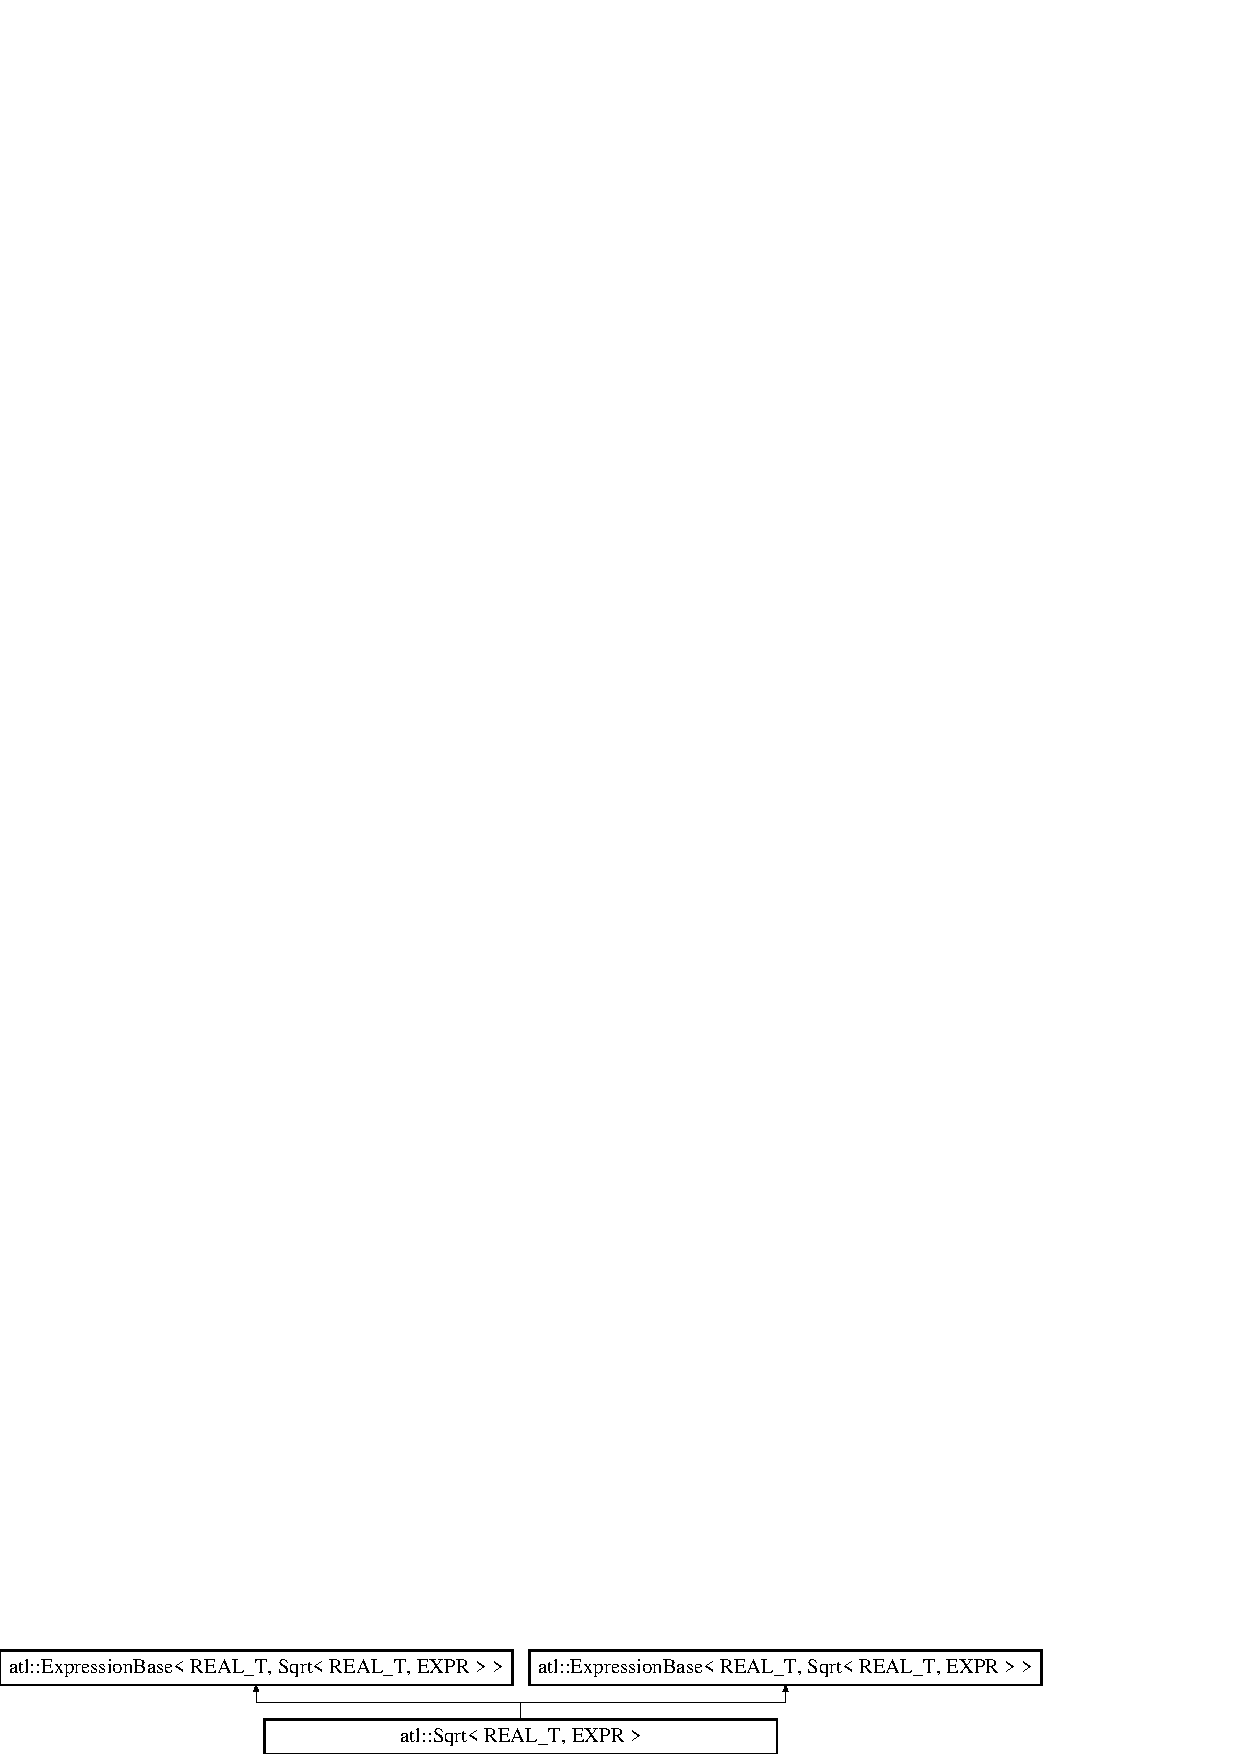
\includegraphics[height=1.637427cm]{structatl_1_1_sqrt}
\end{center}
\end{figure}
\subsection*{Public Types}
\begin{DoxyCompactItemize}
\item 
\hypertarget{structatl_1_1_sqrt_a5f665ddd001904f2bf54c0b30359ee17}{typedef R\+E\+A\+L\+\_\+\+T {\bfseries B\+A\+S\+E\+\_\+\+T\+Y\+P\+E}}\label{structatl_1_1_sqrt_a5f665ddd001904f2bf54c0b30359ee17}

\item 
\hypertarget{structatl_1_1_sqrt_a5f665ddd001904f2bf54c0b30359ee17}{typedef R\+E\+A\+L\+\_\+\+T {\bfseries B\+A\+S\+E\+\_\+\+T\+Y\+P\+E}}\label{structatl_1_1_sqrt_a5f665ddd001904f2bf54c0b30359ee17}

\end{DoxyCompactItemize}
\subsection*{Public Member Functions}
\begin{DoxyCompactItemize}
\item 
\hypertarget{structatl_1_1_sqrt_ac8e3a110ca40bdf839670082dc5e4ef0}{{\bfseries Sqrt} (const \hyperlink{structatl_1_1_expression_base}{Expression\+Base}$<$ R\+E\+A\+L\+\_\+\+T, E\+X\+P\+R $>$ \&a)}\label{structatl_1_1_sqrt_ac8e3a110ca40bdf839670082dc5e4ef0}

\item 
\hypertarget{structatl_1_1_sqrt_a6c0d48a0e6e86b70b7514b750fcb30be}{const R\+E\+A\+L\+\_\+\+T {\bfseries Get\+Value} () const }\label{structatl_1_1_sqrt_a6c0d48a0e6e86b70b7514b750fcb30be}

\item 
\hypertarget{structatl_1_1_sqrt_a3b8ddd52b949a35e968943d3061895d8}{const R\+E\+A\+L\+\_\+\+T {\bfseries Get\+Value} (size\+\_\+t i, size\+\_\+t j=0) const }\label{structatl_1_1_sqrt_a3b8ddd52b949a35e968943d3061895d8}

\item 
\hypertarget{structatl_1_1_sqrt_a6b88eb004324b1c5ce917b240964b84b}{void {\bfseries Push\+Ids} (typename \hyperlink{structatl_1_1_stack_entry}{atl\+::\+Stack\+Entry}$<$ R\+E\+A\+L\+\_\+\+T $>$\+::vi\+\_\+storage \&ids) const }\label{structatl_1_1_sqrt_a6b88eb004324b1c5ce917b240964b84b}

\item 
\hypertarget{structatl_1_1_sqrt_a5aa440d7850741d3f82e4c82156bdc57}{void {\bfseries Push\+Ids} (typename \hyperlink{structatl_1_1_stack_entry}{atl\+::\+Stack\+Entry}$<$ R\+E\+A\+L\+\_\+\+T $>$\+::vi\+\_\+storage \&ids, size\+\_\+t i, size\+\_\+t j=0) const }\label{structatl_1_1_sqrt_a5aa440d7850741d3f82e4c82156bdc57}

\item 
\hypertarget{structatl_1_1_sqrt_a2f172626c37c28171e634ba3eeba348f}{const R\+E\+A\+L\+\_\+\+T {\bfseries Evaluate\+Derivative} (uint32\+\_\+t id) const }\label{structatl_1_1_sqrt_a2f172626c37c28171e634ba3eeba348f}

\item 
\hypertarget{structatl_1_1_sqrt_a0557e6c7ac21f2fe378119fd68a52bdd}{R\+E\+A\+L\+\_\+\+T {\bfseries Evaluate\+Derivative} (uint32\+\_\+t a, uint32\+\_\+t b) const }\label{structatl_1_1_sqrt_a0557e6c7ac21f2fe378119fd68a52bdd}

\item 
\hypertarget{structatl_1_1_sqrt_ab6c9c3321b4f641ea4059c9c26308238}{R\+E\+A\+L\+\_\+\+T {\bfseries Evaluate\+Derivative} (uint32\+\_\+t x, uint32\+\_\+t y, uint32\+\_\+t z) const }\label{structatl_1_1_sqrt_ab6c9c3321b4f641ea4059c9c26308238}

\item 
\hypertarget{structatl_1_1_sqrt_a5b341ed635d616c4ee7b9520c6beaf67}{const R\+E\+A\+L\+\_\+\+T {\bfseries Evaluate\+Derivative} (uint32\+\_\+t id, size\+\_\+t i, size\+\_\+t j=0) const }\label{structatl_1_1_sqrt_a5b341ed635d616c4ee7b9520c6beaf67}

\item 
\hypertarget{structatl_1_1_sqrt_a03db61c5b7ff56d7a58c05c11b8618f9}{R\+E\+A\+L\+\_\+\+T {\bfseries Evaluate\+Derivative} (uint32\+\_\+t a, uint32\+\_\+t b, size\+\_\+t i, size\+\_\+t j=0) const }\label{structatl_1_1_sqrt_a03db61c5b7ff56d7a58c05c11b8618f9}

\item 
\hypertarget{structatl_1_1_sqrt_abe56609f5a775fcba0d98645013e30bf}{R\+E\+A\+L\+\_\+\+T {\bfseries Evaluate\+Derivative} (uint32\+\_\+t x, uint32\+\_\+t y, uint32\+\_\+t z, size\+\_\+t i, size\+\_\+t j=0) const }\label{structatl_1_1_sqrt_abe56609f5a775fcba0d98645013e30bf}

\item 
\hypertarget{structatl_1_1_sqrt_a896ef6daaf446b8c314858a15a6688cf}{size\+\_\+t {\bfseries Get\+Columns} () const }\label{structatl_1_1_sqrt_a896ef6daaf446b8c314858a15a6688cf}

\item 
\hypertarget{structatl_1_1_sqrt_abfa08333fc04697ea542b1399a4aa491}{size\+\_\+t {\bfseries Get\+Rows} () const }\label{structatl_1_1_sqrt_abfa08333fc04697ea542b1399a4aa491}

\item 
\hypertarget{structatl_1_1_sqrt_aa075ea8b91dbb80539905f5803df09fd}{bool {\bfseries Is\+Scalar} () const }\label{structatl_1_1_sqrt_aa075ea8b91dbb80539905f5803df09fd}

\item 
\hyperlink{structatl_1_1_sqrt_ac8e3a110ca40bdf839670082dc5e4ef0}{Sqrt} (const \hyperlink{structatl_1_1_expression_base}{Expression\+Base}$<$ R\+E\+A\+L\+\_\+\+T, E\+X\+P\+R $>$ \&a)
\item 
const R\+E\+A\+L\+\_\+\+T \hyperlink{structatl_1_1_sqrt_a6c0d48a0e6e86b70b7514b750fcb30be}{Get\+Value} () const 
\item 
const R\+E\+A\+L\+\_\+\+T \hyperlink{structatl_1_1_sqrt_a3b8ddd52b949a35e968943d3061895d8}{Get\+Value} (size\+\_\+t i, size\+\_\+t j=0) const 
\item 
bool \hyperlink{structatl_1_1_sqrt_a476ac8bdcd0ce6652813615910dc9447}{Is\+Nonlinear} () const 
\item 
void \hyperlink{structatl_1_1_sqrt_a6b88eb004324b1c5ce917b240964b84b}{Push\+Ids} (typename \hyperlink{structatl_1_1_stack_entry}{atl\+::\+Stack\+Entry}$<$ R\+E\+A\+L\+\_\+\+T $>$\+::vi\+\_\+storage \&ids) const 
\item 
void \hyperlink{structatl_1_1_sqrt_a5aa440d7850741d3f82e4c82156bdc57}{Push\+Ids} (typename \hyperlink{structatl_1_1_stack_entry}{atl\+::\+Stack\+Entry}$<$ R\+E\+A\+L\+\_\+\+T $>$\+::vi\+\_\+storage \&ids, size\+\_\+t i, size\+\_\+t j=0) const 
\item 
const R\+E\+A\+L\+\_\+\+T \hyperlink{structatl_1_1_sqrt_ad947337b0d33abfb9fe7e671a3a6b01b}{Evaluate\+Derivative} (uint32\+\_\+t x) const 
\item 
R\+E\+A\+L\+\_\+\+T \hyperlink{structatl_1_1_sqrt_a96f53e404e169b1c69d063fefcb8176b}{Evaluate\+Derivative} (uint32\+\_\+t x, uint32\+\_\+t y) const 
\item 
R\+E\+A\+L\+\_\+\+T \hyperlink{structatl_1_1_sqrt_ab6c9c3321b4f641ea4059c9c26308238}{Evaluate\+Derivative} (uint32\+\_\+t x, uint32\+\_\+t y, uint32\+\_\+t z) const 
\item 
const R\+E\+A\+L\+\_\+\+T \hyperlink{structatl_1_1_sqrt_a17d66a2d5c04e28ae1f57cfd1bf68c04}{Evaluate\+Derivative} (uint32\+\_\+t x, size\+\_\+t i, size\+\_\+t j=0) const 
\item 
R\+E\+A\+L\+\_\+\+T \hyperlink{structatl_1_1_sqrt_affa365598724b7e0f8f0ef2d2653af9f}{Evaluate\+Derivative} (uint32\+\_\+t x, uint32\+\_\+t y, size\+\_\+t i, size\+\_\+t j=0) const 
\item 
R\+E\+A\+L\+\_\+\+T \hyperlink{structatl_1_1_sqrt_abe56609f5a775fcba0d98645013e30bf}{Evaluate\+Derivative} (uint32\+\_\+t x, uint32\+\_\+t y, uint32\+\_\+t z, size\+\_\+t i, size\+\_\+t j=0) const 
\item 
size\+\_\+t \hyperlink{structatl_1_1_sqrt_abfa08333fc04697ea542b1399a4aa491}{Get\+Rows} () const 
\item 
bool \hyperlink{structatl_1_1_sqrt_aa075ea8b91dbb80539905f5803df09fd}{Is\+Scalar} () const 
\item 
const std\+::string \hyperlink{structatl_1_1_sqrt_a6459cdf71df9ccae80fbf884fa1d2808}{To\+Expression\+Template\+String} () const 
\end{DoxyCompactItemize}
\subsection*{Public Attributes}
\begin{DoxyCompactItemize}
\item 
\hypertarget{structatl_1_1_sqrt_a66500fe8a464dc483f7776969a153356}{const E\+X\+P\+R \& {\bfseries expr\+\_\+m}}\label{structatl_1_1_sqrt_a66500fe8a464dc483f7776969a153356}

\end{DoxyCompactItemize}


\subsection{Detailed Description}
\subsubsection*{template$<$class R\+E\+A\+L\+\_\+\+T, class E\+X\+P\+R$>$struct atl\+::\+Sqrt$<$ R\+E\+A\+L\+\_\+\+T, E\+X\+P\+R $>$}

Expression template to handle square root of a variable or container expressions.

$ \sqrt f(x) $

or

$ \sqrt f_{i,j}(x) $ 

\subsection{Constructor \& Destructor Documentation}
\hypertarget{structatl_1_1_sqrt_ac8e3a110ca40bdf839670082dc5e4ef0}{\index{atl\+::\+Sqrt@{atl\+::\+Sqrt}!Sqrt@{Sqrt}}
\index{Sqrt@{Sqrt}!atl\+::\+Sqrt@{atl\+::\+Sqrt}}
\subsubsection[{Sqrt}]{\setlength{\rightskip}{0pt plus 5cm}template$<$class R\+E\+A\+L\+\_\+\+T , class E\+X\+P\+R $>$ {\bf atl\+::\+Sqrt}$<$ R\+E\+A\+L\+\_\+\+T, E\+X\+P\+R $>$\+::{\bf Sqrt} (
\begin{DoxyParamCaption}
\item[{const {\bf Expression\+Base}$<$ R\+E\+A\+L\+\_\+\+T, E\+X\+P\+R $>$ \&}]{a}
\end{DoxyParamCaption}
)\hspace{0.3cm}{\ttfamily [inline]}}}\label{structatl_1_1_sqrt_ac8e3a110ca40bdf839670082dc5e4ef0}
Constructor 
\begin{DoxyParams}{Parameters}
{\em a} & \\
\hline
\end{DoxyParams}


\subsection{Member Function Documentation}
\hypertarget{structatl_1_1_sqrt_ad947337b0d33abfb9fe7e671a3a6b01b}{\index{atl\+::\+Sqrt@{atl\+::\+Sqrt}!Evaluate\+Derivative@{Evaluate\+Derivative}}
\index{Evaluate\+Derivative@{Evaluate\+Derivative}!atl\+::\+Sqrt@{atl\+::\+Sqrt}}
\subsubsection[{Evaluate\+Derivative}]{\setlength{\rightskip}{0pt plus 5cm}template$<$class R\+E\+A\+L\+\_\+\+T , class E\+X\+P\+R $>$ const R\+E\+A\+L\+\_\+\+T {\bf atl\+::\+Sqrt}$<$ R\+E\+A\+L\+\_\+\+T, E\+X\+P\+R $>$\+::Evaluate\+Derivative (
\begin{DoxyParamCaption}
\item[{uint32\+\_\+t}]{x}
\end{DoxyParamCaption}
) const\hspace{0.3cm}{\ttfamily [inline]}}}\label{structatl_1_1_sqrt_ad947337b0d33abfb9fe7e671a3a6b01b}
Evaluates the first-\/order derivative with respect to x.

$ {{{{d}\over{d\,x}}\,f(x)}\over{2\,\sqrt{f(x)}}} $


\begin{DoxyParams}{Parameters}
{\em x} & \\
\hline
\end{DoxyParams}
\begin{DoxyReturn}{Returns}

\end{DoxyReturn}
\hypertarget{structatl_1_1_sqrt_a96f53e404e169b1c69d063fefcb8176b}{\index{atl\+::\+Sqrt@{atl\+::\+Sqrt}!Evaluate\+Derivative@{Evaluate\+Derivative}}
\index{Evaluate\+Derivative@{Evaluate\+Derivative}!atl\+::\+Sqrt@{atl\+::\+Sqrt}}
\subsubsection[{Evaluate\+Derivative}]{\setlength{\rightskip}{0pt plus 5cm}template$<$class R\+E\+A\+L\+\_\+\+T , class E\+X\+P\+R $>$ R\+E\+A\+L\+\_\+\+T {\bf atl\+::\+Sqrt}$<$ R\+E\+A\+L\+\_\+\+T, E\+X\+P\+R $>$\+::Evaluate\+Derivative (
\begin{DoxyParamCaption}
\item[{uint32\+\_\+t}]{x, }
\item[{uint32\+\_\+t}]{y}
\end{DoxyParamCaption}
) const\hspace{0.3cm}{\ttfamily [inline]}}}\label{structatl_1_1_sqrt_a96f53e404e169b1c69d063fefcb8176b}
Evaluates the second-\/order derivative with respect to x and y.

$ {{{{d^2}\over{d\,x\,d\,y}}\,f(x,y)}\over{2\,\sqrt{f(x,y )}}}-{{{{d}\over{d\,x}}\,f(x,y)\,\left({{d}\over{d\,y}}\, f(x,y)\right)}\over{4\,f(x,y)^{{{3}\over{2}}}}} $


\begin{DoxyParams}{Parameters}
{\em x} & \\
\hline
{\em y} & \\
\hline
\end{DoxyParams}
\begin{DoxyReturn}{Returns}

\end{DoxyReturn}
\hypertarget{structatl_1_1_sqrt_ab6c9c3321b4f641ea4059c9c26308238}{\index{atl\+::\+Sqrt@{atl\+::\+Sqrt}!Evaluate\+Derivative@{Evaluate\+Derivative}}
\index{Evaluate\+Derivative@{Evaluate\+Derivative}!atl\+::\+Sqrt@{atl\+::\+Sqrt}}
\subsubsection[{Evaluate\+Derivative}]{\setlength{\rightskip}{0pt plus 5cm}template$<$class R\+E\+A\+L\+\_\+\+T , class E\+X\+P\+R $>$ R\+E\+A\+L\+\_\+\+T {\bf atl\+::\+Sqrt}$<$ R\+E\+A\+L\+\_\+\+T, E\+X\+P\+R $>$\+::Evaluate\+Derivative (
\begin{DoxyParamCaption}
\item[{uint32\+\_\+t}]{x, }
\item[{uint32\+\_\+t}]{y, }
\item[{uint32\+\_\+t}]{z}
\end{DoxyParamCaption}
) const\hspace{0.3cm}{\ttfamily [inline]}}}\label{structatl_1_1_sqrt_ab6c9c3321b4f641ea4059c9c26308238}
Evaluates the third-\/order derivative with respect to x, y, and z.

$ {{3\,\left({{d}\over{d\,x}}\,f(x,y,z)\right)\,\left({{d }\over{d\,y}}\,f(x,y,z)\right)\,\left({{d}\over{d\,z}}\,f_{i,j }(x,y,z)\right)}\over{8\,f(x,y,z)^{{{5}\over{2}}}}}-{{{{d^2 }\over{d\,x\,d\,y}}\,f(x,y,z)\,\left({{d}\over{d\,z}}\,f (x,y,z)\right)}\over{4\,f(x,y,z)^{{{3}\over{2}}}}}-{{{{d }\over{d\,x}}\,f(x,y,z)\,\left({{d^2}\over{d\,y\,d\,z}}\,f_{i, j}(x,y,z)\right)}\over{4\,f(x,y,z)^{{{3}\over{2}}}}}-{{{{d^2 }\over{d\,x\,d\,z}}\,f(x,y,z)\,\left({{d}\over{d\,y}}\,f (x,y,z)\right)}\over{4\,f(x,y,z)^{{{3}\over{2}}}}}+{{{{d^3 }\over{d\,x\,d\,y\,d\,z}}\,f(x,y,z)}\over{2\,\sqrt{f(x,y ,z)}}} $


\begin{DoxyParams}{Parameters}
{\em x} & \\
\hline
{\em y} & \\
\hline
{\em z} & \\
\hline
\end{DoxyParams}
\begin{DoxyReturn}{Returns}

\end{DoxyReturn}
\hypertarget{structatl_1_1_sqrt_a17d66a2d5c04e28ae1f57cfd1bf68c04}{\index{atl\+::\+Sqrt@{atl\+::\+Sqrt}!Evaluate\+Derivative@{Evaluate\+Derivative}}
\index{Evaluate\+Derivative@{Evaluate\+Derivative}!atl\+::\+Sqrt@{atl\+::\+Sqrt}}
\subsubsection[{Evaluate\+Derivative}]{\setlength{\rightskip}{0pt plus 5cm}template$<$class R\+E\+A\+L\+\_\+\+T , class E\+X\+P\+R $>$ const R\+E\+A\+L\+\_\+\+T {\bf atl\+::\+Sqrt}$<$ R\+E\+A\+L\+\_\+\+T, E\+X\+P\+R $>$\+::Evaluate\+Derivative (
\begin{DoxyParamCaption}
\item[{uint32\+\_\+t}]{x, }
\item[{size\+\_\+t}]{i, }
\item[{size\+\_\+t}]{j = {\ttfamily 0}}
\end{DoxyParamCaption}
) const\hspace{0.3cm}{\ttfamily [inline]}}}\label{structatl_1_1_sqrt_a17d66a2d5c04e28ae1f57cfd1bf68c04}
Evaluates the first-\/order derivative with respect to x at index \{i,j\}.

$ {{{{d}\over{d\,x}}\,f_{i,j}(x)}\over{2\,\sqrt{f_{i,j}(x)}}} $


\begin{DoxyParams}{Parameters}
{\em x} & \\
\hline
{\em i} & \\
\hline
{\em j} & \\
\hline
\end{DoxyParams}
\begin{DoxyReturn}{Returns}

\end{DoxyReturn}
\hypertarget{structatl_1_1_sqrt_affa365598724b7e0f8f0ef2d2653af9f}{\index{atl\+::\+Sqrt@{atl\+::\+Sqrt}!Evaluate\+Derivative@{Evaluate\+Derivative}}
\index{Evaluate\+Derivative@{Evaluate\+Derivative}!atl\+::\+Sqrt@{atl\+::\+Sqrt}}
\subsubsection[{Evaluate\+Derivative}]{\setlength{\rightskip}{0pt plus 5cm}template$<$class R\+E\+A\+L\+\_\+\+T , class E\+X\+P\+R $>$ R\+E\+A\+L\+\_\+\+T {\bf atl\+::\+Sqrt}$<$ R\+E\+A\+L\+\_\+\+T, E\+X\+P\+R $>$\+::Evaluate\+Derivative (
\begin{DoxyParamCaption}
\item[{uint32\+\_\+t}]{x, }
\item[{uint32\+\_\+t}]{y, }
\item[{size\+\_\+t}]{i, }
\item[{size\+\_\+t}]{j = {\ttfamily 0}}
\end{DoxyParamCaption}
) const\hspace{0.3cm}{\ttfamily [inline]}}}\label{structatl_1_1_sqrt_affa365598724b7e0f8f0ef2d2653af9f}
Evaluates the second-\/order derivative with respect to x and y at index \{i,j\}.

$ {{{{d^2}\over{d\,x\,d\,y}}\,f_{i,j}(x,y)}\over{2\,\sqrt{f_{i,j}(x,y )}}}-{{{{d}\over{d\,x}}\,f_{i,j}(x,y)\,\left({{d}\over{d\,y}}\,f_{i, j}(x,y)\right)}\over{4\,f_{i,j}(x,y)^{{{3}\over{2}}}}} $


\begin{DoxyParams}{Parameters}
{\em x} & \\
\hline
{\em y} & \\
\hline
{\em i} & \\
\hline
{\em j} & \\
\hline
\end{DoxyParams}
\begin{DoxyReturn}{Returns}

\end{DoxyReturn}
\hypertarget{structatl_1_1_sqrt_abe56609f5a775fcba0d98645013e30bf}{\index{atl\+::\+Sqrt@{atl\+::\+Sqrt}!Evaluate\+Derivative@{Evaluate\+Derivative}}
\index{Evaluate\+Derivative@{Evaluate\+Derivative}!atl\+::\+Sqrt@{atl\+::\+Sqrt}}
\subsubsection[{Evaluate\+Derivative}]{\setlength{\rightskip}{0pt plus 5cm}template$<$class R\+E\+A\+L\+\_\+\+T , class E\+X\+P\+R $>$ R\+E\+A\+L\+\_\+\+T {\bf atl\+::\+Sqrt}$<$ R\+E\+A\+L\+\_\+\+T, E\+X\+P\+R $>$\+::Evaluate\+Derivative (
\begin{DoxyParamCaption}
\item[{uint32\+\_\+t}]{x, }
\item[{uint32\+\_\+t}]{y, }
\item[{uint32\+\_\+t}]{z, }
\item[{size\+\_\+t}]{i, }
\item[{size\+\_\+t}]{j = {\ttfamily 0}}
\end{DoxyParamCaption}
) const\hspace{0.3cm}{\ttfamily [inline]}}}\label{structatl_1_1_sqrt_abe56609f5a775fcba0d98645013e30bf}
Evaluates the third-\/order derivative with respect to x, y, and z at index \{i,j\}.

$ {{3\,\left({{d}\over{d\,x}}\,f_{i,j}(x,y,z)\right)\,\left({{d }\over{d\,y}}\,f_{i,j}(x,y,z)\right)\,\left({{d}\over{d\,z}}\,f_{i,j }(x,y,z)\right)}\over{8\,f_{i,j}(x,y,z)^{{{5}\over{2}}}}}-{{{{d^2 }\over{d\,x\,d\,y}}\,f_{i,j}(x,y,z)\,\left({{d}\over{d\,z}}\,f_{i,j} (x,y,z)\right)}\over{4\,f_{i,j}(x,y,z)^{{{3}\over{2}}}}}-{{{{d }\over{d\,x}}\,f_{i,j}(x,y,z)\,\left({{d^2}\over{d\,y\,d\,z}}\,f_{i, j}(x,y,z)\right)}\over{4\,f_{i,j}(x,y,z)^{{{3}\over{2}}}}}-{{{{d^2 }\over{d\,x\,d\,z}}\,f_{i,j}(x,y,z)\,\left({{d}\over{d\,y}}\,f_{i,j} (x,y,z)\right)}\over{4\,f_{i,j}(x,y,z)^{{{3}\over{2}}}}}+{{{{d^3 }\over{d\,x\,d\,y\,d\,z}}\,f_{i,j}(x,y,z)}\over{2\,\sqrt{f_{i,j}(x,y ,z)}}} $


\begin{DoxyParams}{Parameters}
{\em x} & \\
\hline
{\em y} & \\
\hline
{\em z} & \\
\hline
{\em i} & \\
\hline
{\em j} & \\
\hline
\end{DoxyParams}
\begin{DoxyReturn}{Returns}

\end{DoxyReturn}
\hypertarget{structatl_1_1_sqrt_abfa08333fc04697ea542b1399a4aa491}{\index{atl\+::\+Sqrt@{atl\+::\+Sqrt}!Get\+Rows@{Get\+Rows}}
\index{Get\+Rows@{Get\+Rows}!atl\+::\+Sqrt@{atl\+::\+Sqrt}}
\subsubsection[{Get\+Rows}]{\setlength{\rightskip}{0pt plus 5cm}template$<$class R\+E\+A\+L\+\_\+\+T , class E\+X\+P\+R $>$ size\+\_\+t {\bf atl\+::\+Sqrt}$<$ R\+E\+A\+L\+\_\+\+T, E\+X\+P\+R $>$\+::Get\+Rows (
\begin{DoxyParamCaption}
{}
\end{DoxyParamCaption}
) const\hspace{0.3cm}{\ttfamily [inline]}}}\label{structatl_1_1_sqrt_abfa08333fc04697ea542b1399a4aa491}
Return the number of rows.

\begin{DoxyReturn}{Returns}

\end{DoxyReturn}
\hypertarget{structatl_1_1_sqrt_a6c0d48a0e6e86b70b7514b750fcb30be}{\index{atl\+::\+Sqrt@{atl\+::\+Sqrt}!Get\+Value@{Get\+Value}}
\index{Get\+Value@{Get\+Value}!atl\+::\+Sqrt@{atl\+::\+Sqrt}}
\subsubsection[{Get\+Value}]{\setlength{\rightskip}{0pt plus 5cm}template$<$class R\+E\+A\+L\+\_\+\+T , class E\+X\+P\+R $>$ const R\+E\+A\+L\+\_\+\+T {\bf atl\+::\+Sqrt}$<$ R\+E\+A\+L\+\_\+\+T, E\+X\+P\+R $>$\+::Get\+Value (
\begin{DoxyParamCaption}
{}
\end{DoxyParamCaption}
) const\hspace{0.3cm}{\ttfamily [inline]}}}\label{structatl_1_1_sqrt_a6c0d48a0e6e86b70b7514b750fcb30be}
Compute the square root of the evaluated expression.

\begin{DoxyReturn}{Returns}

\end{DoxyReturn}
\hypertarget{structatl_1_1_sqrt_a3b8ddd52b949a35e968943d3061895d8}{\index{atl\+::\+Sqrt@{atl\+::\+Sqrt}!Get\+Value@{Get\+Value}}
\index{Get\+Value@{Get\+Value}!atl\+::\+Sqrt@{atl\+::\+Sqrt}}
\subsubsection[{Get\+Value}]{\setlength{\rightskip}{0pt plus 5cm}template$<$class R\+E\+A\+L\+\_\+\+T , class E\+X\+P\+R $>$ const R\+E\+A\+L\+\_\+\+T {\bf atl\+::\+Sqrt}$<$ R\+E\+A\+L\+\_\+\+T, E\+X\+P\+R $>$\+::Get\+Value (
\begin{DoxyParamCaption}
\item[{size\+\_\+t}]{i, }
\item[{size\+\_\+t}]{j = {\ttfamily 0}}
\end{DoxyParamCaption}
) const\hspace{0.3cm}{\ttfamily [inline]}}}\label{structatl_1_1_sqrt_a3b8ddd52b949a35e968943d3061895d8}
Compute the square root of the evaluated expression at index \{i,j\}.

\begin{DoxyReturn}{Returns}

\end{DoxyReturn}
\hypertarget{structatl_1_1_sqrt_a476ac8bdcd0ce6652813615910dc9447}{\index{atl\+::\+Sqrt@{atl\+::\+Sqrt}!Is\+Nonlinear@{Is\+Nonlinear}}
\index{Is\+Nonlinear@{Is\+Nonlinear}!atl\+::\+Sqrt@{atl\+::\+Sqrt}}
\subsubsection[{Is\+Nonlinear}]{\setlength{\rightskip}{0pt plus 5cm}template$<$class R\+E\+A\+L\+\_\+\+T , class E\+X\+P\+R $>$ bool {\bf atl\+::\+Sqrt}$<$ R\+E\+A\+L\+\_\+\+T, E\+X\+P\+R $>$\+::Is\+Nonlinear (
\begin{DoxyParamCaption}
{}
\end{DoxyParamCaption}
) const\hspace{0.3cm}{\ttfamily [inline]}}}\label{structatl_1_1_sqrt_a476ac8bdcd0ce6652813615910dc9447}
Returns true.

\begin{DoxyReturn}{Returns}

\end{DoxyReturn}
\hypertarget{structatl_1_1_sqrt_aa075ea8b91dbb80539905f5803df09fd}{\index{atl\+::\+Sqrt@{atl\+::\+Sqrt}!Is\+Scalar@{Is\+Scalar}}
\index{Is\+Scalar@{Is\+Scalar}!atl\+::\+Sqrt@{atl\+::\+Sqrt}}
\subsubsection[{Is\+Scalar}]{\setlength{\rightskip}{0pt plus 5cm}template$<$class R\+E\+A\+L\+\_\+\+T , class E\+X\+P\+R $>$ bool {\bf atl\+::\+Sqrt}$<$ R\+E\+A\+L\+\_\+\+T, E\+X\+P\+R $>$\+::Is\+Scalar (
\begin{DoxyParamCaption}
{}
\end{DoxyParamCaption}
) const\hspace{0.3cm}{\ttfamily [inline]}}}\label{structatl_1_1_sqrt_aa075ea8b91dbb80539905f5803df09fd}
True if this expression is a scalar.

\begin{DoxyReturn}{Returns}

\end{DoxyReturn}
\hypertarget{structatl_1_1_sqrt_a6b88eb004324b1c5ce917b240964b84b}{\index{atl\+::\+Sqrt@{atl\+::\+Sqrt}!Push\+Ids@{Push\+Ids}}
\index{Push\+Ids@{Push\+Ids}!atl\+::\+Sqrt@{atl\+::\+Sqrt}}
\subsubsection[{Push\+Ids}]{\setlength{\rightskip}{0pt plus 5cm}template$<$class R\+E\+A\+L\+\_\+\+T , class E\+X\+P\+R $>$ void {\bf atl\+::\+Sqrt}$<$ R\+E\+A\+L\+\_\+\+T, E\+X\+P\+R $>$\+::Push\+Ids (
\begin{DoxyParamCaption}
\item[{typename {\bf atl\+::\+Stack\+Entry}$<$ R\+E\+A\+L\+\_\+\+T $>$\+::vi\+\_\+storage \&}]{ids}
\end{DoxyParamCaption}
) const\hspace{0.3cm}{\ttfamily [inline]}}}\label{structatl_1_1_sqrt_a6b88eb004324b1c5ce917b240964b84b}
Push variable info into a set.


\begin{DoxyParams}{Parameters}
{\em ids} & \\
\hline
\end{DoxyParams}
\hypertarget{structatl_1_1_sqrt_a5aa440d7850741d3f82e4c82156bdc57}{\index{atl\+::\+Sqrt@{atl\+::\+Sqrt}!Push\+Ids@{Push\+Ids}}
\index{Push\+Ids@{Push\+Ids}!atl\+::\+Sqrt@{atl\+::\+Sqrt}}
\subsubsection[{Push\+Ids}]{\setlength{\rightskip}{0pt plus 5cm}template$<$class R\+E\+A\+L\+\_\+\+T , class E\+X\+P\+R $>$ void {\bf atl\+::\+Sqrt}$<$ R\+E\+A\+L\+\_\+\+T, E\+X\+P\+R $>$\+::Push\+Ids (
\begin{DoxyParamCaption}
\item[{typename {\bf atl\+::\+Stack\+Entry}$<$ R\+E\+A\+L\+\_\+\+T $>$\+::vi\+\_\+storage \&}]{ids, }
\item[{size\+\_\+t}]{i, }
\item[{size\+\_\+t}]{j = {\ttfamily 0}}
\end{DoxyParamCaption}
) const\hspace{0.3cm}{\ttfamily [inline]}}}\label{structatl_1_1_sqrt_a5aa440d7850741d3f82e4c82156bdc57}
Push variable info into a set at index \{i,j\}.


\begin{DoxyParams}{Parameters}
{\em ids} & \\
\hline
{\em i} & \\
\hline
{\em j} & \\
\hline
\end{DoxyParams}
\hypertarget{structatl_1_1_sqrt_a6459cdf71df9ccae80fbf884fa1d2808}{\index{atl\+::\+Sqrt@{atl\+::\+Sqrt}!To\+Expression\+Template\+String@{To\+Expression\+Template\+String}}
\index{To\+Expression\+Template\+String@{To\+Expression\+Template\+String}!atl\+::\+Sqrt@{atl\+::\+Sqrt}}
\subsubsection[{To\+Expression\+Template\+String}]{\setlength{\rightskip}{0pt plus 5cm}template$<$class R\+E\+A\+L\+\_\+\+T , class E\+X\+P\+R $>$ const std\+::string {\bf atl\+::\+Sqrt}$<$ R\+E\+A\+L\+\_\+\+T, E\+X\+P\+R $>$\+::To\+Expression\+Template\+String (
\begin{DoxyParamCaption}
{}
\end{DoxyParamCaption}
) const\hspace{0.3cm}{\ttfamily [inline]}}}\label{structatl_1_1_sqrt_a6459cdf71df9ccae80fbf884fa1d2808}
Create a string representation of this expression template. \begin{DoxyReturn}{Returns}

\end{DoxyReturn}


The documentation for this struct was generated from the following file\+:\begin{DoxyCompactItemize}
\item 
A\+T\+L2/Sqrt.\+hpp\end{DoxyCompactItemize}

\hypertarget{structatl_1_1_stack_entry}{\section{atl\+:\+:Stack\+Entry$<$ R\+E\+A\+L\+\_\+\+T $>$ Struct Template Reference}
\label{structatl_1_1_stack_entry}\index{atl\+::\+Stack\+Entry$<$ R\+E\+A\+L\+\_\+\+T $>$@{atl\+::\+Stack\+Entry$<$ R\+E\+A\+L\+\_\+\+T $>$}}
}
\subsection*{Public Types}
\begin{DoxyCompactItemize}
\item 
\hypertarget{structatl_1_1_stack_entry_a094fab5acbe8dc310c222375fed1b6fe}{typedef std\+::set$<$ \hyperlink{structatl_1_1_variable_info}{Variable\+Info}\\*
$<$ R\+E\+A\+L\+\_\+\+T $>$ $\ast$ $>$ {\bfseries vi\+\_\+storage}}\label{structatl_1_1_stack_entry_a094fab5acbe8dc310c222375fed1b6fe}

\item 
\hypertarget{structatl_1_1_stack_entry_a70322748648b26684961de7ce20cc1d0}{typedef vi\+\_\+storage\+::iterator {\bfseries vi\+\_\+iterator}}\label{structatl_1_1_stack_entry_a70322748648b26684961de7ce20cc1d0}

\item 
\hypertarget{structatl_1_1_stack_entry_a094fab5acbe8dc310c222375fed1b6fe}{typedef std\+::set$<$ \hyperlink{structatl_1_1_variable_info}{Variable\+Info}\\*
$<$ R\+E\+A\+L\+\_\+\+T $>$ $\ast$ $>$ {\bfseries vi\+\_\+storage}}\label{structatl_1_1_stack_entry_a094fab5acbe8dc310c222375fed1b6fe}

\item 
\hypertarget{structatl_1_1_stack_entry_a70322748648b26684961de7ce20cc1d0}{typedef vi\+\_\+storage\+::iterator {\bfseries vi\+\_\+iterator}}\label{structatl_1_1_stack_entry_a70322748648b26684961de7ce20cc1d0}

\end{DoxyCompactItemize}
\subsection*{Public Member Functions}
\begin{DoxyCompactItemize}
\item 
\hypertarget{structatl_1_1_stack_entry_a52c0538f3015b76293ea30b70e17db83}{{\bfseries Stack\+Entry} (const \hyperlink{structatl_1_1_stack_entry}{Stack\+Entry}$<$ R\+E\+A\+L\+\_\+\+T $>$ \&other)}\label{structatl_1_1_stack_entry_a52c0538f3015b76293ea30b70e17db83}

\item 
\hypertarget{structatl_1_1_stack_entry_a52c0538f3015b76293ea30b70e17db83}{{\bfseries Stack\+Entry} (const \hyperlink{structatl_1_1_stack_entry}{Stack\+Entry}$<$ R\+E\+A\+L\+\_\+\+T $>$ \&other)}\label{structatl_1_1_stack_entry_a52c0538f3015b76293ea30b70e17db83}

\item 
void \hyperlink{structatl_1_1_stack_entry_a0415bc91dd9e863fb4dd3f7b4d9b05d9}{Push} (\hyperlink{structatl_1_1_variable_info}{Variable\+Info}$<$ R\+E\+A\+L\+\_\+\+T $>$ $\ast$id)
\item 
void \hyperlink{structatl_1_1_stack_entry_a362647e782982e9acd1117d7f5ce4331}{Prepare} ()
\item 
void \hyperlink{structatl_1_1_stack_entry_a47e6f692a3a508a721f87af9797fc15c}{Reset} ()
\end{DoxyCompactItemize}
\subsection*{Public Attributes}
\begin{DoxyCompactItemize}
\item 
\hypertarget{structatl_1_1_stack_entry_a030b94a3c6f50f8ea60126deca7c6cc7}{\hyperlink{structatl_1_1_variable_info}{Variable\+Info}$<$ R\+E\+A\+L\+\_\+\+T $>$ $\ast$ {\bfseries w}}\label{structatl_1_1_stack_entry_a030b94a3c6f50f8ea60126deca7c6cc7}

\item 
\hypertarget{structatl_1_1_stack_entry_a6c7e421af4df1bba1ce5031eec6049b8}{std\+::set$<$ \hyperlink{structatl_1_1_variable_info}{Variable\+Info}$<$ R\+E\+A\+L\+\_\+\+T $>$ $\ast$ $>$ {\bfseries ids}}\label{structatl_1_1_stack_entry_a6c7e421af4df1bba1ce5031eec6049b8}

\item 
\hypertarget{structatl_1_1_stack_entry_ad3ff8babc7ef2524394b6367e8b99d50}{std\+::vector$<$ R\+E\+A\+L\+\_\+\+T $>$ {\bfseries first}}\label{structatl_1_1_stack_entry_ad3ff8babc7ef2524394b6367e8b99d50}

\item 
\hypertarget{structatl_1_1_stack_entry_a5f71d407983c8818ea4baf94113ca4d6}{std\+::vector$<$ R\+E\+A\+L\+\_\+\+T $>$ {\bfseries second}}\label{structatl_1_1_stack_entry_a5f71d407983c8818ea4baf94113ca4d6}

\item 
\hypertarget{structatl_1_1_stack_entry_a5003b4571917fc9ba489b618146fdc03}{std\+::vector$<$ R\+E\+A\+L\+\_\+\+T $>$ {\bfseries third}}\label{structatl_1_1_stack_entry_a5003b4571917fc9ba489b618146fdc03}

\item 
\hypertarget{structatl_1_1_stack_entry_ad787906516faf9b0560e9a05ad498002}{bool {\bfseries is\+\_\+nl}}\label{structatl_1_1_stack_entry_ad787906516faf9b0560e9a05ad498002}

\item 
\hypertarget{structatl_1_1_stack_entry_a4a62fa58ea18326679a6ad6eb3204dbc}{vi\+\_\+storage {\bfseries ids}}\label{structatl_1_1_stack_entry_a4a62fa58ea18326679a6ad6eb3204dbc}

\item 
\hypertarget{structatl_1_1_stack_entry_a73c36c099806680fc64ed05a3ab2e087}{vi\+\_\+storage {\bfseries pushed\+\_\+ids}}\label{structatl_1_1_stack_entry_a73c36c099806680fc64ed05a3ab2e087}

\item 
\hypertarget{structatl_1_1_stack_entry_a756881e857efb10407762e29c5953c44}{std\+::vector$<$ \hyperlink{structatl_1_1_variable_info}{Variable\+Info}\\*
$<$ R\+E\+A\+L\+\_\+\+T $>$ $\ast$ $>$ {\bfseries id\+\_\+list}}\label{structatl_1_1_stack_entry_a756881e857efb10407762e29c5953c44}

\end{DoxyCompactItemize}


\subsection{Member Function Documentation}
\hypertarget{structatl_1_1_stack_entry_a362647e782982e9acd1117d7f5ce4331}{\index{atl\+::\+Stack\+Entry@{atl\+::\+Stack\+Entry}!Prepare@{Prepare}}
\index{Prepare@{Prepare}!atl\+::\+Stack\+Entry@{atl\+::\+Stack\+Entry}}
\subsubsection[{Prepare}]{\setlength{\rightskip}{0pt plus 5cm}template$<$typename R\+E\+A\+L\+\_\+\+T$>$ void {\bf atl\+::\+Stack\+Entry}$<$ R\+E\+A\+L\+\_\+\+T $>$\+::Prepare (
\begin{DoxyParamCaption}
{}
\end{DoxyParamCaption}
)\hspace{0.3cm}{\ttfamily [inline]}}}\label{structatl_1_1_stack_entry_a362647e782982e9acd1117d7f5ce4331}
Prepares this entry for evaluation. \hypertarget{structatl_1_1_stack_entry_a0415bc91dd9e863fb4dd3f7b4d9b05d9}{\index{atl\+::\+Stack\+Entry@{atl\+::\+Stack\+Entry}!Push@{Push}}
\index{Push@{Push}!atl\+::\+Stack\+Entry@{atl\+::\+Stack\+Entry}}
\subsubsection[{Push}]{\setlength{\rightskip}{0pt plus 5cm}template$<$typename R\+E\+A\+L\+\_\+\+T$>$ void {\bf atl\+::\+Stack\+Entry}$<$ R\+E\+A\+L\+\_\+\+T $>$\+::Push (
\begin{DoxyParamCaption}
\item[{{\bf Variable\+Info}$<$ R\+E\+A\+L\+\_\+\+T $>$ $\ast$}]{id}
\end{DoxyParamCaption}
)\hspace{0.3cm}{\ttfamily [inline]}}}\label{structatl_1_1_stack_entry_a0415bc91dd9e863fb4dd3f7b4d9b05d9}
Push an id into this entry. Used for higher-\/order derivatives.


\begin{DoxyParams}{Parameters}
{\em id} & \\
\hline
\end{DoxyParams}
\hypertarget{structatl_1_1_stack_entry_a47e6f692a3a508a721f87af9797fc15c}{\index{atl\+::\+Stack\+Entry@{atl\+::\+Stack\+Entry}!Reset@{Reset}}
\index{Reset@{Reset}!atl\+::\+Stack\+Entry@{atl\+::\+Stack\+Entry}}
\subsubsection[{Reset}]{\setlength{\rightskip}{0pt plus 5cm}template$<$typename R\+E\+A\+L\+\_\+\+T$>$ void {\bf atl\+::\+Stack\+Entry}$<$ R\+E\+A\+L\+\_\+\+T $>$\+::Reset (
\begin{DoxyParamCaption}
{}
\end{DoxyParamCaption}
)\hspace{0.3cm}{\ttfamily [inline]}}}\label{structatl_1_1_stack_entry_a47e6f692a3a508a721f87af9797fc15c}
Reset this entry. 

The documentation for this struct was generated from the following file\+:\begin{DoxyCompactItemize}
\item 
A\+T\+L2/Tape.\+hpp\end{DoxyCompactItemize}

\hypertarget{classatl_1_1_streamed_data_file}{\section{atl\+:\+:Streamed\+Data\+File Class Reference}
\label{classatl_1_1_streamed_data_file}\index{atl\+::\+Streamed\+Data\+File@{atl\+::\+Streamed\+Data\+File}}
}
\subsection*{Public Member Functions}
\begin{DoxyCompactItemize}
\item 
\hypertarget{classatl_1_1_streamed_data_file_a6e67c20c6c9cadc73c8b1f03aa718d02}{{\bfseries Streamed\+Data\+File} (const char $\ast$path)}\label{classatl_1_1_streamed_data_file_a6e67c20c6c9cadc73c8b1f03aa718d02}

\item 
\hypertarget{classatl_1_1_streamed_data_file_a3b2671f133e8a530d98ac590580c6096}{void {\bfseries open} (const char $\ast$path)}\label{classatl_1_1_streamed_data_file_a3b2671f133e8a530d98ac590580c6096}

\item 
\hypertarget{classatl_1_1_streamed_data_file_a527cb3ee0f344dc0c4ac97294e191abc}{bool {\bfseries good} ()}\label{classatl_1_1_streamed_data_file_a527cb3ee0f344dc0c4ac97294e191abc}

\item 
\hypertarget{classatl_1_1_streamed_data_file_a22b5623bf585d73489dad501eab354a2}{void {\bfseries operator$>$$>$} (char $\ast$v)}\label{classatl_1_1_streamed_data_file_a22b5623bf585d73489dad501eab354a2}

\item 
\hypertarget{classatl_1_1_streamed_data_file_ad26d2083f90178d75dc92f81bb57c441}{void {\bfseries operator$>$$>$} (unsigned char $\ast$v)}\label{classatl_1_1_streamed_data_file_ad26d2083f90178d75dc92f81bb57c441}

\item 
\hypertarget{classatl_1_1_streamed_data_file_aa4ffdabdad2333b34b72ea0e60008b79}{void {\bfseries operator$>$$>$} (signed char $\ast$v)}\label{classatl_1_1_streamed_data_file_aa4ffdabdad2333b34b72ea0e60008b79}

\item 
\hypertarget{classatl_1_1_streamed_data_file_a35195c6a64047382340b12bc0b00df0b}{void {\bfseries operator$>$$>$} (char \&v)}\label{classatl_1_1_streamed_data_file_a35195c6a64047382340b12bc0b00df0b}

\item 
\hypertarget{classatl_1_1_streamed_data_file_a01306b5166e5c01dca4db8c1d7e9a9b1}{void {\bfseries operator$>$$>$} (unsigned char \&v)}\label{classatl_1_1_streamed_data_file_a01306b5166e5c01dca4db8c1d7e9a9b1}

\item 
\hypertarget{classatl_1_1_streamed_data_file_acc4879d12886f287e5b3ef04188dd7f0}{void {\bfseries operator$>$$>$} (signed char \&v)}\label{classatl_1_1_streamed_data_file_acc4879d12886f287e5b3ef04188dd7f0}

\item 
\hypertarget{classatl_1_1_streamed_data_file_a5972df17588b27d7ac8d6bf13191574f}{void {\bfseries operator$>$$>$} (int \&v)}\label{classatl_1_1_streamed_data_file_a5972df17588b27d7ac8d6bf13191574f}

\item 
\hypertarget{classatl_1_1_streamed_data_file_aa54e9305c39c8d7a8312d866f2bff0e2}{void {\bfseries operator$>$$>$} (long \&v)}\label{classatl_1_1_streamed_data_file_aa54e9305c39c8d7a8312d866f2bff0e2}

\item 
\hypertarget{classatl_1_1_streamed_data_file_a4af2c4bb06589880887abebe28f7270a}{void {\bfseries operator$>$$>$} (short \&v)}\label{classatl_1_1_streamed_data_file_a4af2c4bb06589880887abebe28f7270a}

\item 
\hypertarget{classatl_1_1_streamed_data_file_a1e19495966936e7f64bc643ef6eaf8f3}{void {\bfseries operator$>$$>$} (unsigned int \&v)}\label{classatl_1_1_streamed_data_file_a1e19495966936e7f64bc643ef6eaf8f3}

\item 
\hypertarget{classatl_1_1_streamed_data_file_ac51480891b04387ad3daa2b56ff5fec6}{void {\bfseries operator$>$$>$} (unsigned long \&v)}\label{classatl_1_1_streamed_data_file_ac51480891b04387ad3daa2b56ff5fec6}

\item 
\hypertarget{classatl_1_1_streamed_data_file_a29bc30cf68e2704d3deae37252f3ca4b}{void {\bfseries operator$>$$>$} (unsigned short \&v)}\label{classatl_1_1_streamed_data_file_a29bc30cf68e2704d3deae37252f3ca4b}

\item 
\hypertarget{classatl_1_1_streamed_data_file_a557c30c9b789c70c4fa33058d2720aa5}{void {\bfseries operator$>$$>$} (bool \&v)}\label{classatl_1_1_streamed_data_file_a557c30c9b789c70c4fa33058d2720aa5}

\item 
\hypertarget{classatl_1_1_streamed_data_file_a1927ecf5f6fb12a6ae3ab6ed7a9d479b}{void {\bfseries operator$>$$>$} (float \&v)}\label{classatl_1_1_streamed_data_file_a1927ecf5f6fb12a6ae3ab6ed7a9d479b}

\item 
\hypertarget{classatl_1_1_streamed_data_file_ac29592c8193459c0289a712712d8df3f}{void {\bfseries operator$>$$>$} (double \&v)}\label{classatl_1_1_streamed_data_file_ac29592c8193459c0289a712712d8df3f}

\item 
\hypertarget{classatl_1_1_streamed_data_file_aefb6dc4e7e31bf2aa1e5691228cee31f}{void {\bfseries operator$>$$>$} (long double \&v)}\label{classatl_1_1_streamed_data_file_aefb6dc4e7e31bf2aa1e5691228cee31f}

\item 
\hypertarget{classatl_1_1_streamed_data_file_a2fbe46b06b1947c479afd3ac2627f87c}{void {\bfseries operator$>$$>$} (std\+::string \&v)}\label{classatl_1_1_streamed_data_file_a2fbe46b06b1947c479afd3ac2627f87c}

\end{DoxyCompactItemize}


The documentation for this class was generated from the following file\+:\begin{DoxyCompactItemize}
\item 
Utilities/\+I\+O/Streamed\+Data\+File.\+hpp\end{DoxyCompactItemize}

\hypertarget{structatl_1_1_subtract}{\section{atl\+:\+:Subtract$<$ R\+E\+A\+L\+\_\+\+T, L\+H\+S, R\+H\+S $>$ Struct Template Reference}
\label{structatl_1_1_subtract}\index{atl\+::\+Subtract$<$ R\+E\+A\+L\+\_\+\+T, L\+H\+S, R\+H\+S $>$@{atl\+::\+Subtract$<$ R\+E\+A\+L\+\_\+\+T, L\+H\+S, R\+H\+S $>$}}
}


{\ttfamily \#include $<$Subtract.\+hpp$>$}

Inheritance diagram for atl\+:\+:Subtract$<$ R\+E\+A\+L\+\_\+\+T, L\+H\+S, R\+H\+S $>$\+:\begin{figure}[H]
\begin{center}
\leavevmode
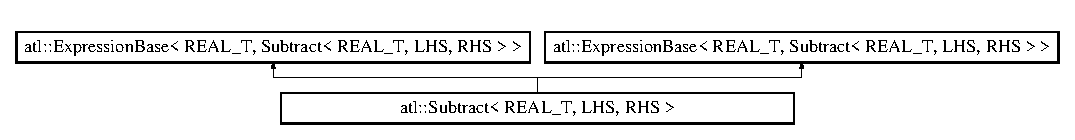
\includegraphics[height=1.428571cm]{structatl_1_1_subtract}
\end{center}
\end{figure}
\subsection*{Public Types}
\begin{DoxyCompactItemize}
\item 
\hypertarget{structatl_1_1_subtract_a55824989e3eac095ebab0f24e7bf49da}{typedef R\+E\+A\+L\+\_\+\+T {\bfseries B\+A\+S\+E\+\_\+\+T\+Y\+P\+E}}\label{structatl_1_1_subtract_a55824989e3eac095ebab0f24e7bf49da}

\item 
\hypertarget{structatl_1_1_subtract_a55824989e3eac095ebab0f24e7bf49da}{typedef R\+E\+A\+L\+\_\+\+T {\bfseries B\+A\+S\+E\+\_\+\+T\+Y\+P\+E}}\label{structatl_1_1_subtract_a55824989e3eac095ebab0f24e7bf49da}

\end{DoxyCompactItemize}
\subsection*{Public Member Functions}
\begin{DoxyCompactItemize}
\item 
\hypertarget{structatl_1_1_subtract_a5aa723f31391e747b2e0ad15119534a7}{{\bfseries Subtract} (const \hyperlink{structatl_1_1_expression_base}{Expression\+Base}$<$ R\+E\+A\+L\+\_\+\+T, L\+H\+S $>$ \&lhs, const \hyperlink{structatl_1_1_expression_base}{Expression\+Base}$<$ R\+E\+A\+L\+\_\+\+T, R\+H\+S $>$ \&rhs)}\label{structatl_1_1_subtract_a5aa723f31391e747b2e0ad15119534a7}

\item 
\hypertarget{structatl_1_1_subtract_aec4aa20754729e6982fcf50cc8db62f0}{{\bfseries Subtract} (const R\+E\+A\+L\+\_\+\+T \&lhs, const \hyperlink{structatl_1_1_expression_base}{Expression\+Base}$<$ R\+E\+A\+L\+\_\+\+T, R\+H\+S $>$ \&rhs)}\label{structatl_1_1_subtract_aec4aa20754729e6982fcf50cc8db62f0}

\item 
\hypertarget{structatl_1_1_subtract_a62685c3f4f2009e2d8d5d456b6fadc99}{{\bfseries Subtract} (const \hyperlink{structatl_1_1_expression_base}{Expression\+Base}$<$ R\+E\+A\+L\+\_\+\+T, L\+H\+S $>$ \&lhs, const R\+E\+A\+L\+\_\+\+T \&rhs)}\label{structatl_1_1_subtract_a62685c3f4f2009e2d8d5d456b6fadc99}

\item 
\hypertarget{structatl_1_1_subtract_a80b7e3ae7a1459a1a64f226dbc6007db}{const R\+E\+A\+L\+\_\+\+T {\bfseries Get\+Value} () const }\label{structatl_1_1_subtract_a80b7e3ae7a1459a1a64f226dbc6007db}

\item 
\hypertarget{structatl_1_1_subtract_a88c1c9bc7979105b03e33e12e7c68fe1}{const R\+E\+A\+L\+\_\+\+T {\bfseries Get\+Value} (size\+\_\+t i, size\+\_\+t j=0) const }\label{structatl_1_1_subtract_a88c1c9bc7979105b03e33e12e7c68fe1}

\item 
\hypertarget{structatl_1_1_subtract_a975412a952c1ac7e416b240c1d26e1f7}{void {\bfseries Push\+Ids} (typename \hyperlink{structatl_1_1_stack_entry}{atl\+::\+Stack\+Entry}$<$ R\+E\+A\+L\+\_\+\+T $>$\+::vi\+\_\+storage \&ids) const }\label{structatl_1_1_subtract_a975412a952c1ac7e416b240c1d26e1f7}

\item 
\hypertarget{structatl_1_1_subtract_aa1e7d93e4b4a9bf0a1f60e9e214b3d3c}{void {\bfseries Push\+Ids} (typename \hyperlink{structatl_1_1_stack_entry}{atl\+::\+Stack\+Entry}$<$ R\+E\+A\+L\+\_\+\+T $>$\+::vi\+\_\+storage \&ids, size\+\_\+t i, size\+\_\+t j=0) const }\label{structatl_1_1_subtract_aa1e7d93e4b4a9bf0a1f60e9e214b3d3c}

\item 
\hypertarget{structatl_1_1_subtract_a1c024b42eec6f0b9bb60062f2a05fe60}{R\+E\+A\+L\+\_\+\+T {\bfseries Evaluate\+Derivative} (uint32\+\_\+t a) const }\label{structatl_1_1_subtract_a1c024b42eec6f0b9bb60062f2a05fe60}

\item 
\hypertarget{structatl_1_1_subtract_a8108d862d6282c0476c4fb5529233d50}{R\+E\+A\+L\+\_\+\+T {\bfseries Evaluate\+Derivative} (uint32\+\_\+t a, uint32\+\_\+t b) const }\label{structatl_1_1_subtract_a8108d862d6282c0476c4fb5529233d50}

\item 
\hypertarget{structatl_1_1_subtract_a1284210aba1ac90b41818eb93be2e097}{R\+E\+A\+L\+\_\+\+T {\bfseries Evaluate\+Derivative} (uint32\+\_\+t x, uint32\+\_\+t y, uint32\+\_\+t z) const }\label{structatl_1_1_subtract_a1284210aba1ac90b41818eb93be2e097}

\item 
\hypertarget{structatl_1_1_subtract_a2defe6bbcc739bbdd872fd23bdbb2306}{R\+E\+A\+L\+\_\+\+T {\bfseries Evaluate\+Derivative} (uint32\+\_\+t a, size\+\_\+t i, size\+\_\+t j=0) const }\label{structatl_1_1_subtract_a2defe6bbcc739bbdd872fd23bdbb2306}

\item 
\hypertarget{structatl_1_1_subtract_a6ca805f54a4cef65edb46507a208f732}{R\+E\+A\+L\+\_\+\+T {\bfseries Evaluate\+Derivative} (uint32\+\_\+t a, uint32\+\_\+t b, size\+\_\+t i, size\+\_\+t j=0) const }\label{structatl_1_1_subtract_a6ca805f54a4cef65edb46507a208f732}

\item 
\hypertarget{structatl_1_1_subtract_ae9ca2e237fac48dd380435215a8bc224}{R\+E\+A\+L\+\_\+\+T {\bfseries Evaluate\+Derivative} (uint32\+\_\+t x, uint32\+\_\+t y, uint32\+\_\+t z, size\+\_\+t i, size\+\_\+t j=0) const }\label{structatl_1_1_subtract_ae9ca2e237fac48dd380435215a8bc224}

\item 
\hypertarget{structatl_1_1_subtract_a855cb338fa3c5b1abd2c3ef7076d3da6}{size\+\_\+t {\bfseries Get\+Columns} () const }\label{structatl_1_1_subtract_a855cb338fa3c5b1abd2c3ef7076d3da6}

\item 
\hypertarget{structatl_1_1_subtract_a3178686169bc6c020f6191f0e1d89887}{size\+\_\+t {\bfseries Get\+Rows} () const }\label{structatl_1_1_subtract_a3178686169bc6c020f6191f0e1d89887}

\item 
\hypertarget{structatl_1_1_subtract_a230ee7ae322737b12c84136e534a5624}{bool {\bfseries Is\+Scalar} () const }\label{structatl_1_1_subtract_a230ee7ae322737b12c84136e534a5624}

\item 
\hyperlink{structatl_1_1_subtract_a5aa723f31391e747b2e0ad15119534a7}{Subtract} (const \hyperlink{structatl_1_1_expression_base}{Expression\+Base}$<$ R\+E\+A\+L\+\_\+\+T, L\+H\+S $>$ \&lhs, const \hyperlink{structatl_1_1_expression_base}{Expression\+Base}$<$ R\+E\+A\+L\+\_\+\+T, R\+H\+S $>$ \&rhs)
\item 
\hyperlink{structatl_1_1_subtract_aec4aa20754729e6982fcf50cc8db62f0}{Subtract} (const R\+E\+A\+L\+\_\+\+T \&lhs, const \hyperlink{structatl_1_1_expression_base}{Expression\+Base}$<$ R\+E\+A\+L\+\_\+\+T, R\+H\+S $>$ \&rhs)
\item 
\hyperlink{structatl_1_1_subtract_a62685c3f4f2009e2d8d5d456b6fadc99}{Subtract} (const \hyperlink{structatl_1_1_expression_base}{Expression\+Base}$<$ R\+E\+A\+L\+\_\+\+T, L\+H\+S $>$ \&lhs, const R\+E\+A\+L\+\_\+\+T \&rhs)
\item 
const R\+E\+A\+L\+\_\+\+T \hyperlink{structatl_1_1_subtract_a80b7e3ae7a1459a1a64f226dbc6007db}{Get\+Value} () const 
\item 
const R\+E\+A\+L\+\_\+\+T \hyperlink{structatl_1_1_subtract_a88c1c9bc7979105b03e33e12e7c68fe1}{Get\+Value} (size\+\_\+t i, size\+\_\+t j=0) const 
\item 
bool \hyperlink{structatl_1_1_subtract_a74f23d9df17503bf6c83b753b5ba3fa1}{Is\+Nonlinear} () const 
\item 
void \hyperlink{structatl_1_1_subtract_a975412a952c1ac7e416b240c1d26e1f7}{Push\+Ids} (typename \hyperlink{structatl_1_1_stack_entry}{atl\+::\+Stack\+Entry}$<$ R\+E\+A\+L\+\_\+\+T $>$\+::vi\+\_\+storage \&ids) const 
\item 
void \hyperlink{structatl_1_1_subtract_aa1e7d93e4b4a9bf0a1f60e9e214b3d3c}{Push\+Ids} (typename \hyperlink{structatl_1_1_stack_entry}{atl\+::\+Stack\+Entry}$<$ R\+E\+A\+L\+\_\+\+T $>$\+::vi\+\_\+storage \&ids, size\+\_\+t i, size\+\_\+t j=0) const 
\item 
R\+E\+A\+L\+\_\+\+T \hyperlink{structatl_1_1_subtract_aeae21f80058270d778c731dda78dabfc}{Evaluate\+Derivative} (uint32\+\_\+t x) const 
\item 
R\+E\+A\+L\+\_\+\+T \hyperlink{structatl_1_1_subtract_adc7933999b1ea0f040b983ad02c8a7b6}{Evaluate\+Derivative} (uint32\+\_\+t x, uint32\+\_\+t y) const 
\item 
R\+E\+A\+L\+\_\+\+T \hyperlink{structatl_1_1_subtract_a1284210aba1ac90b41818eb93be2e097}{Evaluate\+Derivative} (uint32\+\_\+t x, uint32\+\_\+t y, uint32\+\_\+t z) const 
\item 
R\+E\+A\+L\+\_\+\+T \hyperlink{structatl_1_1_subtract_aff679c6ebb81a9c0caf5dc1400cfb718}{Evaluate\+Derivative} (uint32\+\_\+t x, size\+\_\+t i, size\+\_\+t j=0) const 
\item 
R\+E\+A\+L\+\_\+\+T \hyperlink{structatl_1_1_subtract_aa1c554a245afa879ebab6e68f592bb90}{Evaluate\+Derivative} (uint32\+\_\+t x, uint32\+\_\+t y, size\+\_\+t i, size\+\_\+t j=0) const 
\item 
R\+E\+A\+L\+\_\+\+T \hyperlink{structatl_1_1_subtract_ae9ca2e237fac48dd380435215a8bc224}{Evaluate\+Derivative} (uint32\+\_\+t x, uint32\+\_\+t y, uint32\+\_\+t z, size\+\_\+t i, size\+\_\+t j=0) const 
\item 
size\+\_\+t \hyperlink{structatl_1_1_subtract_a855cb338fa3c5b1abd2c3ef7076d3da6}{Get\+Columns} () const 
\item 
size\+\_\+t \hyperlink{structatl_1_1_subtract_a3178686169bc6c020f6191f0e1d89887}{Get\+Rows} () const 
\item 
bool \hyperlink{structatl_1_1_subtract_a230ee7ae322737b12c84136e534a5624}{Is\+Scalar} () const 
\item 
const std\+::string \hyperlink{structatl_1_1_subtract_a5282da95ee1c8d921dc17e642ce20d94}{To\+Expression\+Template\+String} () const 
\end{DoxyCompactItemize}
\subsection*{Public Attributes}
\begin{DoxyCompactItemize}
\item 
\hypertarget{structatl_1_1_subtract_a418b68d42f9655c3e579e2f41430c680}{\hyperlink{structatl_1_1_real}{atl\+::\+Real}$<$ R\+E\+A\+L\+\_\+\+T $>$ {\bfseries real\+\_\+m}}\label{structatl_1_1_subtract_a418b68d42f9655c3e579e2f41430c680}

\item 
\hypertarget{structatl_1_1_subtract_a50d122ada13d9dcec017d3428e1a8895}{const L\+H\+S \& {\bfseries lhs\+\_\+m}}\label{structatl_1_1_subtract_a50d122ada13d9dcec017d3428e1a8895}

\item 
\hypertarget{structatl_1_1_subtract_a51c853273f222f5c2c7c23bd6c46cea9}{const R\+H\+S \& {\bfseries rhs\+\_\+m}}\label{structatl_1_1_subtract_a51c853273f222f5c2c7c23bd6c46cea9}

\item 
\hypertarget{structatl_1_1_subtract_ae074418a06e7fed14d436cac9edd8f8d}{R\+E\+A\+L\+\_\+\+T {\bfseries value\+\_\+m}}\label{structatl_1_1_subtract_ae074418a06e7fed14d436cac9edd8f8d}

\end{DoxyCompactItemize}


\subsection{Detailed Description}
\subsubsection*{template$<$class R\+E\+A\+L\+\_\+\+T, class L\+H\+S, class R\+H\+S$>$struct atl\+::\+Subtract$<$ R\+E\+A\+L\+\_\+\+T, L\+H\+S, R\+H\+S $>$}

Expression template to handle subtraction.

$ f(x) - g(x) $

or

$ f_{i,j}(x) - g_{i,j}(x) $ 

\subsection{Constructor \& Destructor Documentation}
\hypertarget{structatl_1_1_subtract_a5aa723f31391e747b2e0ad15119534a7}{\index{atl\+::\+Subtract@{atl\+::\+Subtract}!Subtract@{Subtract}}
\index{Subtract@{Subtract}!atl\+::\+Subtract@{atl\+::\+Subtract}}
\subsubsection[{Subtract}]{\setlength{\rightskip}{0pt plus 5cm}template$<$class R\+E\+A\+L\+\_\+\+T, class L\+H\+S , class R\+H\+S $>$ {\bf atl\+::\+Subtract}$<$ R\+E\+A\+L\+\_\+\+T, L\+H\+S, R\+H\+S $>$\+::{\bf Subtract} (
\begin{DoxyParamCaption}
\item[{const {\bf Expression\+Base}$<$ R\+E\+A\+L\+\_\+\+T, L\+H\+S $>$ \&}]{lhs, }
\item[{const {\bf Expression\+Base}$<$ R\+E\+A\+L\+\_\+\+T, R\+H\+S $>$ \&}]{rhs}
\end{DoxyParamCaption}
)\hspace{0.3cm}{\ttfamily [inline]}}}\label{structatl_1_1_subtract_a5aa723f31391e747b2e0ad15119534a7}
Constructor for two variable types.


\begin{DoxyParams}{Parameters}
{\em lhs} & \\
\hline
{\em rhs} & \\
\hline
\end{DoxyParams}
\hypertarget{structatl_1_1_subtract_aec4aa20754729e6982fcf50cc8db62f0}{\index{atl\+::\+Subtract@{atl\+::\+Subtract}!Subtract@{Subtract}}
\index{Subtract@{Subtract}!atl\+::\+Subtract@{atl\+::\+Subtract}}
\subsubsection[{Subtract}]{\setlength{\rightskip}{0pt plus 5cm}template$<$class R\+E\+A\+L\+\_\+\+T, class L\+H\+S , class R\+H\+S $>$ {\bf atl\+::\+Subtract}$<$ R\+E\+A\+L\+\_\+\+T, L\+H\+S, R\+H\+S $>$\+::{\bf Subtract} (
\begin{DoxyParamCaption}
\item[{const R\+E\+A\+L\+\_\+\+T \&}]{lhs, }
\item[{const {\bf Expression\+Base}$<$ R\+E\+A\+L\+\_\+\+T, R\+H\+S $>$ \&}]{rhs}
\end{DoxyParamCaption}
)\hspace{0.3cm}{\ttfamily [inline]}}}\label{structatl_1_1_subtract_aec4aa20754729e6982fcf50cc8db62f0}
Constructor for real plus variable type. \hypertarget{structatl_1_1_subtract_a62685c3f4f2009e2d8d5d456b6fadc99}{\index{atl\+::\+Subtract@{atl\+::\+Subtract}!Subtract@{Subtract}}
\index{Subtract@{Subtract}!atl\+::\+Subtract@{atl\+::\+Subtract}}
\subsubsection[{Subtract}]{\setlength{\rightskip}{0pt plus 5cm}template$<$class R\+E\+A\+L\+\_\+\+T, class L\+H\+S , class R\+H\+S $>$ {\bf atl\+::\+Subtract}$<$ R\+E\+A\+L\+\_\+\+T, L\+H\+S, R\+H\+S $>$\+::{\bf Subtract} (
\begin{DoxyParamCaption}
\item[{const {\bf Expression\+Base}$<$ R\+E\+A\+L\+\_\+\+T, L\+H\+S $>$ \&}]{lhs, }
\item[{const R\+E\+A\+L\+\_\+\+T \&}]{rhs}
\end{DoxyParamCaption}
)\hspace{0.3cm}{\ttfamily [inline]}}}\label{structatl_1_1_subtract_a62685c3f4f2009e2d8d5d456b6fadc99}
Constructor for variable plus real type. 
\begin{DoxyParams}{Parameters}
{\em lhs} & \\
\hline
{\em rhs} & \\
\hline
\end{DoxyParams}


\subsection{Member Function Documentation}
\hypertarget{structatl_1_1_subtract_aeae21f80058270d778c731dda78dabfc}{\index{atl\+::\+Subtract@{atl\+::\+Subtract}!Evaluate\+Derivative@{Evaluate\+Derivative}}
\index{Evaluate\+Derivative@{Evaluate\+Derivative}!atl\+::\+Subtract@{atl\+::\+Subtract}}
\subsubsection[{Evaluate\+Derivative}]{\setlength{\rightskip}{0pt plus 5cm}template$<$class R\+E\+A\+L\+\_\+\+T, class L\+H\+S , class R\+H\+S $>$ R\+E\+A\+L\+\_\+\+T {\bf atl\+::\+Subtract}$<$ R\+E\+A\+L\+\_\+\+T, L\+H\+S, R\+H\+S $>$\+::Evaluate\+Derivative (
\begin{DoxyParamCaption}
\item[{uint32\+\_\+t}]{x}
\end{DoxyParamCaption}
) const\hspace{0.3cm}{\ttfamily [inline]}}}\label{structatl_1_1_subtract_aeae21f80058270d778c731dda78dabfc}
Evaluates the first-\/order derivative of this expression with respect to x.

$ {{d}\over{d\,x}}\,f(x)-{{d}\over{d\,x}}\,g(x) $


\begin{DoxyParams}{Parameters}
{\em x} & \\
\hline
\end{DoxyParams}
\begin{DoxyReturn}{Returns}

\end{DoxyReturn}
\hypertarget{structatl_1_1_subtract_adc7933999b1ea0f040b983ad02c8a7b6}{\index{atl\+::\+Subtract@{atl\+::\+Subtract}!Evaluate\+Derivative@{Evaluate\+Derivative}}
\index{Evaluate\+Derivative@{Evaluate\+Derivative}!atl\+::\+Subtract@{atl\+::\+Subtract}}
\subsubsection[{Evaluate\+Derivative}]{\setlength{\rightskip}{0pt plus 5cm}template$<$class R\+E\+A\+L\+\_\+\+T, class L\+H\+S , class R\+H\+S $>$ R\+E\+A\+L\+\_\+\+T {\bf atl\+::\+Subtract}$<$ R\+E\+A\+L\+\_\+\+T, L\+H\+S, R\+H\+S $>$\+::Evaluate\+Derivative (
\begin{DoxyParamCaption}
\item[{uint32\+\_\+t}]{x, }
\item[{uint32\+\_\+t}]{y}
\end{DoxyParamCaption}
) const\hspace{0.3cm}{\ttfamily [inline]}}}\label{structatl_1_1_subtract_adc7933999b1ea0f040b983ad02c8a7b6}
Evaluates the second-\/order derivative with respect to x and y.

$ {{d^2}\over{d\,x\,d\,y}}\,f\left(x , y\right)-{{d^2}\over{d\,x\,d\, y}}\,g\left(x , y\right) $ 
\begin{DoxyParams}{Parameters}
{\em x} & \\
\hline
{\em y} & \\
\hline
\end{DoxyParams}
\begin{DoxyReturn}{Returns}

\end{DoxyReturn}
\hypertarget{structatl_1_1_subtract_a1284210aba1ac90b41818eb93be2e097}{\index{atl\+::\+Subtract@{atl\+::\+Subtract}!Evaluate\+Derivative@{Evaluate\+Derivative}}
\index{Evaluate\+Derivative@{Evaluate\+Derivative}!atl\+::\+Subtract@{atl\+::\+Subtract}}
\subsubsection[{Evaluate\+Derivative}]{\setlength{\rightskip}{0pt plus 5cm}template$<$class R\+E\+A\+L\+\_\+\+T, class L\+H\+S , class R\+H\+S $>$ R\+E\+A\+L\+\_\+\+T {\bf atl\+::\+Subtract}$<$ R\+E\+A\+L\+\_\+\+T, L\+H\+S, R\+H\+S $>$\+::Evaluate\+Derivative (
\begin{DoxyParamCaption}
\item[{uint32\+\_\+t}]{x, }
\item[{uint32\+\_\+t}]{y, }
\item[{uint32\+\_\+t}]{z}
\end{DoxyParamCaption}
) const\hspace{0.3cm}{\ttfamily [inline]}}}\label{structatl_1_1_subtract_a1284210aba1ac90b41818eb93be2e097}
Evaluates the third-\/order derivative with respect to x, y, and z.

$ {{d^2}\over{d\,x\,d\,y}}\,f(x,y)- {{d^2}\over{d\,x\,d\,y}}\,g(x,y) $


\begin{DoxyParams}{Parameters}
{\em x} & \\
\hline
{\em y} & \\
\hline
{\em z} & \\
\hline
\end{DoxyParams}
\begin{DoxyReturn}{Returns}

\end{DoxyReturn}
\hypertarget{structatl_1_1_subtract_aff679c6ebb81a9c0caf5dc1400cfb718}{\index{atl\+::\+Subtract@{atl\+::\+Subtract}!Evaluate\+Derivative@{Evaluate\+Derivative}}
\index{Evaluate\+Derivative@{Evaluate\+Derivative}!atl\+::\+Subtract@{atl\+::\+Subtract}}
\subsubsection[{Evaluate\+Derivative}]{\setlength{\rightskip}{0pt plus 5cm}template$<$class R\+E\+A\+L\+\_\+\+T, class L\+H\+S , class R\+H\+S $>$ R\+E\+A\+L\+\_\+\+T {\bf atl\+::\+Subtract}$<$ R\+E\+A\+L\+\_\+\+T, L\+H\+S, R\+H\+S $>$\+::Evaluate\+Derivative (
\begin{DoxyParamCaption}
\item[{uint32\+\_\+t}]{x, }
\item[{size\+\_\+t}]{i, }
\item[{size\+\_\+t}]{j = {\ttfamily 0}}
\end{DoxyParamCaption}
) const\hspace{0.3cm}{\ttfamily [inline]}}}\label{structatl_1_1_subtract_aff679c6ebb81a9c0caf5dc1400cfb718}
Evaluates the first-\/order derivative of this expression with respect to x at index \{i,j\}.

$ {{d}\over{d\,x}}\,f(x)-{{d}\over{d\,x}}\,g(x) $


\begin{DoxyParams}{Parameters}
{\em x} & \\
\hline
{\em i} & \\
\hline
{\em j} & \\
\hline
\end{DoxyParams}
\begin{DoxyReturn}{Returns}

\end{DoxyReturn}
\hypertarget{structatl_1_1_subtract_aa1c554a245afa879ebab6e68f592bb90}{\index{atl\+::\+Subtract@{atl\+::\+Subtract}!Evaluate\+Derivative@{Evaluate\+Derivative}}
\index{Evaluate\+Derivative@{Evaluate\+Derivative}!atl\+::\+Subtract@{atl\+::\+Subtract}}
\subsubsection[{Evaluate\+Derivative}]{\setlength{\rightskip}{0pt plus 5cm}template$<$class R\+E\+A\+L\+\_\+\+T, class L\+H\+S , class R\+H\+S $>$ R\+E\+A\+L\+\_\+\+T {\bf atl\+::\+Subtract}$<$ R\+E\+A\+L\+\_\+\+T, L\+H\+S, R\+H\+S $>$\+::Evaluate\+Derivative (
\begin{DoxyParamCaption}
\item[{uint32\+\_\+t}]{x, }
\item[{uint32\+\_\+t}]{y, }
\item[{size\+\_\+t}]{i, }
\item[{size\+\_\+t}]{j = {\ttfamily 0}}
\end{DoxyParamCaption}
) const\hspace{0.3cm}{\ttfamily [inline]}}}\label{structatl_1_1_subtract_aa1c554a245afa879ebab6e68f592bb90}
Evaluates the second-\/order derivative with respect to x and y at index\{i,j\}.

$ {{d^2}\over{d\,x\,d\,y}}\,f_{i,j}(x,y)-{{d^2}\over{d\,x\,d\,y}}\,g _{i,j}(x,y) $


\begin{DoxyParams}{Parameters}
{\em x} & \\
\hline
{\em y} & \\
\hline
{\em i} & \\
\hline
{\em j} & \\
\hline
\end{DoxyParams}
\begin{DoxyReturn}{Returns}

\end{DoxyReturn}
\hypertarget{structatl_1_1_subtract_ae9ca2e237fac48dd380435215a8bc224}{\index{atl\+::\+Subtract@{atl\+::\+Subtract}!Evaluate\+Derivative@{Evaluate\+Derivative}}
\index{Evaluate\+Derivative@{Evaluate\+Derivative}!atl\+::\+Subtract@{atl\+::\+Subtract}}
\subsubsection[{Evaluate\+Derivative}]{\setlength{\rightskip}{0pt plus 5cm}template$<$class R\+E\+A\+L\+\_\+\+T, class L\+H\+S , class R\+H\+S $>$ R\+E\+A\+L\+\_\+\+T {\bf atl\+::\+Subtract}$<$ R\+E\+A\+L\+\_\+\+T, L\+H\+S, R\+H\+S $>$\+::Evaluate\+Derivative (
\begin{DoxyParamCaption}
\item[{uint32\+\_\+t}]{x, }
\item[{uint32\+\_\+t}]{y, }
\item[{uint32\+\_\+t}]{z, }
\item[{size\+\_\+t}]{i, }
\item[{size\+\_\+t}]{j = {\ttfamily 0}}
\end{DoxyParamCaption}
) const\hspace{0.3cm}{\ttfamily [inline]}}}\label{structatl_1_1_subtract_ae9ca2e237fac48dd380435215a8bc224}
Evaluates the third-\/order derivative with respect to x, y, and z at index \{i,j\}.

$ {{d^3}\over{d\,x\,d\,y\,d\,z}}\,f_{i,j}(x,y,z)-{{d^3}\over{d\,x\,d \,y\,d\,z}}\,g_{i,j}(x,y,z) $


\begin{DoxyParams}{Parameters}
{\em x} & \\
\hline
{\em y} & \\
\hline
{\em z} & \\
\hline
{\em i} & \\
\hline
{\em j} & \\
\hline
\end{DoxyParams}
\begin{DoxyReturn}{Returns}

\end{DoxyReturn}
\hypertarget{structatl_1_1_subtract_a855cb338fa3c5b1abd2c3ef7076d3da6}{\index{atl\+::\+Subtract@{atl\+::\+Subtract}!Get\+Columns@{Get\+Columns}}
\index{Get\+Columns@{Get\+Columns}!atl\+::\+Subtract@{atl\+::\+Subtract}}
\subsubsection[{Get\+Columns}]{\setlength{\rightskip}{0pt plus 5cm}template$<$class R\+E\+A\+L\+\_\+\+T, class L\+H\+S , class R\+H\+S $>$ size\+\_\+t {\bf atl\+::\+Subtract}$<$ R\+E\+A\+L\+\_\+\+T, L\+H\+S, R\+H\+S $>$\+::Get\+Columns (
\begin{DoxyParamCaption}
{}
\end{DoxyParamCaption}
) const\hspace{0.3cm}{\ttfamily [inline]}}}\label{structatl_1_1_subtract_a855cb338fa3c5b1abd2c3ef7076d3da6}
Returns the number of columns.

\begin{DoxyReturn}{Returns}

\end{DoxyReturn}
\hypertarget{structatl_1_1_subtract_a3178686169bc6c020f6191f0e1d89887}{\index{atl\+::\+Subtract@{atl\+::\+Subtract}!Get\+Rows@{Get\+Rows}}
\index{Get\+Rows@{Get\+Rows}!atl\+::\+Subtract@{atl\+::\+Subtract}}
\subsubsection[{Get\+Rows}]{\setlength{\rightskip}{0pt plus 5cm}template$<$class R\+E\+A\+L\+\_\+\+T, class L\+H\+S , class R\+H\+S $>$ size\+\_\+t {\bf atl\+::\+Subtract}$<$ R\+E\+A\+L\+\_\+\+T, L\+H\+S, R\+H\+S $>$\+::Get\+Rows (
\begin{DoxyParamCaption}
{}
\end{DoxyParamCaption}
) const\hspace{0.3cm}{\ttfamily [inline]}}}\label{structatl_1_1_subtract_a3178686169bc6c020f6191f0e1d89887}
Returns the number of rows.

\begin{DoxyReturn}{Returns}

\end{DoxyReturn}
\hypertarget{structatl_1_1_subtract_a80b7e3ae7a1459a1a64f226dbc6007db}{\index{atl\+::\+Subtract@{atl\+::\+Subtract}!Get\+Value@{Get\+Value}}
\index{Get\+Value@{Get\+Value}!atl\+::\+Subtract@{atl\+::\+Subtract}}
\subsubsection[{Get\+Value}]{\setlength{\rightskip}{0pt plus 5cm}template$<$class R\+E\+A\+L\+\_\+\+T, class L\+H\+S , class R\+H\+S $>$ const R\+E\+A\+L\+\_\+\+T {\bf atl\+::\+Subtract}$<$ R\+E\+A\+L\+\_\+\+T, L\+H\+S, R\+H\+S $>$\+::Get\+Value (
\begin{DoxyParamCaption}
{}
\end{DoxyParamCaption}
) const\hspace{0.3cm}{\ttfamily [inline]}}}\label{structatl_1_1_subtract_a80b7e3ae7a1459a1a64f226dbc6007db}
Compute the subtraction of the lhs by the rhs. \begin{DoxyReturn}{Returns}

\end{DoxyReturn}
\hypertarget{structatl_1_1_subtract_a88c1c9bc7979105b03e33e12e7c68fe1}{\index{atl\+::\+Subtract@{atl\+::\+Subtract}!Get\+Value@{Get\+Value}}
\index{Get\+Value@{Get\+Value}!atl\+::\+Subtract@{atl\+::\+Subtract}}
\subsubsection[{Get\+Value}]{\setlength{\rightskip}{0pt plus 5cm}template$<$class R\+E\+A\+L\+\_\+\+T, class L\+H\+S , class R\+H\+S $>$ const R\+E\+A\+L\+\_\+\+T {\bf atl\+::\+Subtract}$<$ R\+E\+A\+L\+\_\+\+T, L\+H\+S, R\+H\+S $>$\+::Get\+Value (
\begin{DoxyParamCaption}
\item[{size\+\_\+t}]{i, }
\item[{size\+\_\+t}]{j = {\ttfamily 0}}
\end{DoxyParamCaption}
) const\hspace{0.3cm}{\ttfamily [inline]}}}\label{structatl_1_1_subtract_a88c1c9bc7979105b03e33e12e7c68fe1}
Compute the subtraction of the lhs by the rhs at index \{i,j\}.

\begin{DoxyReturn}{Returns}

\end{DoxyReturn}
\hypertarget{structatl_1_1_subtract_a74f23d9df17503bf6c83b753b5ba3fa1}{\index{atl\+::\+Subtract@{atl\+::\+Subtract}!Is\+Nonlinear@{Is\+Nonlinear}}
\index{Is\+Nonlinear@{Is\+Nonlinear}!atl\+::\+Subtract@{atl\+::\+Subtract}}
\subsubsection[{Is\+Nonlinear}]{\setlength{\rightskip}{0pt plus 5cm}template$<$class R\+E\+A\+L\+\_\+\+T, class L\+H\+S , class R\+H\+S $>$ bool {\bf atl\+::\+Subtract}$<$ R\+E\+A\+L\+\_\+\+T, L\+H\+S, R\+H\+S $>$\+::Is\+Nonlinear (
\begin{DoxyParamCaption}
{}
\end{DoxyParamCaption}
) const\hspace{0.3cm}{\ttfamily [inline]}}}\label{structatl_1_1_subtract_a74f23d9df17503bf6c83b753b5ba3fa1}
Returns true if the left or right side is nonlinear, else false. \begin{DoxyReturn}{Returns}

\end{DoxyReturn}
\hypertarget{structatl_1_1_subtract_a230ee7ae322737b12c84136e534a5624}{\index{atl\+::\+Subtract@{atl\+::\+Subtract}!Is\+Scalar@{Is\+Scalar}}
\index{Is\+Scalar@{Is\+Scalar}!atl\+::\+Subtract@{atl\+::\+Subtract}}
\subsubsection[{Is\+Scalar}]{\setlength{\rightskip}{0pt plus 5cm}template$<$class R\+E\+A\+L\+\_\+\+T, class L\+H\+S , class R\+H\+S $>$ bool {\bf atl\+::\+Subtract}$<$ R\+E\+A\+L\+\_\+\+T, L\+H\+S, R\+H\+S $>$\+::Is\+Scalar (
\begin{DoxyParamCaption}
{}
\end{DoxyParamCaption}
) const\hspace{0.3cm}{\ttfamily [inline]}}}\label{structatl_1_1_subtract_a230ee7ae322737b12c84136e534a5624}
True if scalar.

\begin{DoxyReturn}{Returns}

\end{DoxyReturn}
\hypertarget{structatl_1_1_subtract_a975412a952c1ac7e416b240c1d26e1f7}{\index{atl\+::\+Subtract@{atl\+::\+Subtract}!Push\+Ids@{Push\+Ids}}
\index{Push\+Ids@{Push\+Ids}!atl\+::\+Subtract@{atl\+::\+Subtract}}
\subsubsection[{Push\+Ids}]{\setlength{\rightskip}{0pt plus 5cm}template$<$class R\+E\+A\+L\+\_\+\+T, class L\+H\+S , class R\+H\+S $>$ void {\bf atl\+::\+Subtract}$<$ R\+E\+A\+L\+\_\+\+T, L\+H\+S, R\+H\+S $>$\+::Push\+Ids (
\begin{DoxyParamCaption}
\item[{typename {\bf atl\+::\+Stack\+Entry}$<$ R\+E\+A\+L\+\_\+\+T $>$\+::vi\+\_\+storage \&}]{ids}
\end{DoxyParamCaption}
) const\hspace{0.3cm}{\ttfamily [inline]}}}\label{structatl_1_1_subtract_a975412a952c1ac7e416b240c1d26e1f7}
Push variable info into a set.


\begin{DoxyParams}{Parameters}
{\em ids} & \\
\hline
\end{DoxyParams}
\hypertarget{structatl_1_1_subtract_aa1e7d93e4b4a9bf0a1f60e9e214b3d3c}{\index{atl\+::\+Subtract@{atl\+::\+Subtract}!Push\+Ids@{Push\+Ids}}
\index{Push\+Ids@{Push\+Ids}!atl\+::\+Subtract@{atl\+::\+Subtract}}
\subsubsection[{Push\+Ids}]{\setlength{\rightskip}{0pt plus 5cm}template$<$class R\+E\+A\+L\+\_\+\+T, class L\+H\+S , class R\+H\+S $>$ void {\bf atl\+::\+Subtract}$<$ R\+E\+A\+L\+\_\+\+T, L\+H\+S, R\+H\+S $>$\+::Push\+Ids (
\begin{DoxyParamCaption}
\item[{typename {\bf atl\+::\+Stack\+Entry}$<$ R\+E\+A\+L\+\_\+\+T $>$\+::vi\+\_\+storage \&}]{ids, }
\item[{size\+\_\+t}]{i, }
\item[{size\+\_\+t}]{j = {\ttfamily 0}}
\end{DoxyParamCaption}
) const\hspace{0.3cm}{\ttfamily [inline]}}}\label{structatl_1_1_subtract_aa1e7d93e4b4a9bf0a1f60e9e214b3d3c}
Push variable info into a set at index \{i,j\}.


\begin{DoxyParams}{Parameters}
{\em ids} & \\
\hline
{\em i} & \\
\hline
{\em j} & \\
\hline
\end{DoxyParams}
\hypertarget{structatl_1_1_subtract_a5282da95ee1c8d921dc17e642ce20d94}{\index{atl\+::\+Subtract@{atl\+::\+Subtract}!To\+Expression\+Template\+String@{To\+Expression\+Template\+String}}
\index{To\+Expression\+Template\+String@{To\+Expression\+Template\+String}!atl\+::\+Subtract@{atl\+::\+Subtract}}
\subsubsection[{To\+Expression\+Template\+String}]{\setlength{\rightskip}{0pt plus 5cm}template$<$class R\+E\+A\+L\+\_\+\+T, class L\+H\+S , class R\+H\+S $>$ const std\+::string {\bf atl\+::\+Subtract}$<$ R\+E\+A\+L\+\_\+\+T, L\+H\+S, R\+H\+S $>$\+::To\+Expression\+Template\+String (
\begin{DoxyParamCaption}
{}
\end{DoxyParamCaption}
) const\hspace{0.3cm}{\ttfamily [inline]}}}\label{structatl_1_1_subtract_a5282da95ee1c8d921dc17e642ce20d94}
Create a string representation of this expression template. \begin{DoxyReturn}{Returns}

\end{DoxyReturn}


The documentation for this struct was generated from the following file\+:\begin{DoxyCompactItemize}
\item 
A\+T\+L2/Subtract.\+hpp\end{DoxyCompactItemize}

\hypertarget{structatl_1_1_tan}{\section{atl\+:\+:Tan$<$ R\+E\+A\+L\+\_\+\+T, E\+X\+P\+R $>$ Struct Template Reference}
\label{structatl_1_1_tan}\index{atl\+::\+Tan$<$ R\+E\+A\+L\+\_\+\+T, E\+X\+P\+R $>$@{atl\+::\+Tan$<$ R\+E\+A\+L\+\_\+\+T, E\+X\+P\+R $>$}}
}


{\ttfamily \#include $<$Tan.\+hpp$>$}

Inheritance diagram for atl\+:\+:Tan$<$ R\+E\+A\+L\+\_\+\+T, E\+X\+P\+R $>$\+:\begin{figure}[H]
\begin{center}
\leavevmode
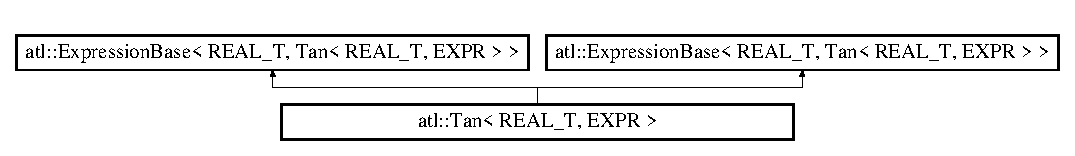
\includegraphics[height=1.642229cm]{structatl_1_1_tan}
\end{center}
\end{figure}
\subsection*{Public Types}
\begin{DoxyCompactItemize}
\item 
\hypertarget{structatl_1_1_tan_aaafd5cb21795f2c493a239df32a10fe9}{typedef R\+E\+A\+L\+\_\+\+T {\bfseries B\+A\+S\+E\+\_\+\+T\+Y\+P\+E}}\label{structatl_1_1_tan_aaafd5cb21795f2c493a239df32a10fe9}

\item 
\hypertarget{structatl_1_1_tan_aaafd5cb21795f2c493a239df32a10fe9}{typedef R\+E\+A\+L\+\_\+\+T {\bfseries B\+A\+S\+E\+\_\+\+T\+Y\+P\+E}}\label{structatl_1_1_tan_aaafd5cb21795f2c493a239df32a10fe9}

\end{DoxyCompactItemize}
\subsection*{Public Member Functions}
\begin{DoxyCompactItemize}
\item 
\hypertarget{structatl_1_1_tan_a009437f9412022ee861a1d36d743ae9d}{{\bfseries Tan} (const \hyperlink{structatl_1_1_expression_base}{Expression\+Base}$<$ R\+E\+A\+L\+\_\+\+T, E\+X\+P\+R $>$ \&a)}\label{structatl_1_1_tan_a009437f9412022ee861a1d36d743ae9d}

\item 
\hypertarget{structatl_1_1_tan_a61807403c56e8851e8c298f88b94d3be}{const R\+E\+A\+L\+\_\+\+T {\bfseries Get\+Value} () const }\label{structatl_1_1_tan_a61807403c56e8851e8c298f88b94d3be}

\item 
\hypertarget{structatl_1_1_tan_a1e1762090976901dc6e79199ed43b309}{const R\+E\+A\+L\+\_\+\+T {\bfseries Get\+Value} (size\+\_\+t i, size\+\_\+t j=0) const }\label{structatl_1_1_tan_a1e1762090976901dc6e79199ed43b309}

\item 
\hypertarget{structatl_1_1_tan_ad4ca7f38ff57eda3d9163cb2bfd6daf3}{void {\bfseries Push\+Ids} (typename \hyperlink{structatl_1_1_stack_entry}{atl\+::\+Stack\+Entry}$<$ R\+E\+A\+L\+\_\+\+T $>$\+::vi\+\_\+storage \&ids) const }\label{structatl_1_1_tan_ad4ca7f38ff57eda3d9163cb2bfd6daf3}

\item 
\hypertarget{structatl_1_1_tan_a39bf4856c2b171188160f0bf7755d6ac}{void {\bfseries Push\+Ids} (typename \hyperlink{structatl_1_1_stack_entry}{atl\+::\+Stack\+Entry}$<$ R\+E\+A\+L\+\_\+\+T $>$\+::vi\+\_\+storage \&ids, size\+\_\+t i, size\+\_\+t j=0) const }\label{structatl_1_1_tan_a39bf4856c2b171188160f0bf7755d6ac}

\item 
\hypertarget{structatl_1_1_tan_a83b6b8d04476e2dff0b23ee6ea41ff3e}{const R\+E\+A\+L\+\_\+\+T {\bfseries Evaluate\+Derivative} (uint32\+\_\+t id) const }\label{structatl_1_1_tan_a83b6b8d04476e2dff0b23ee6ea41ff3e}

\item 
\hypertarget{structatl_1_1_tan_acdc36f314d2d4164e6a7876317c9475a}{R\+E\+A\+L\+\_\+\+T {\bfseries Evaluate\+Derivative} (uint32\+\_\+t a, uint32\+\_\+t b) const }\label{structatl_1_1_tan_acdc36f314d2d4164e6a7876317c9475a}

\item 
\hypertarget{structatl_1_1_tan_a0ae8d9af53301a2dc999eddb8babe4cf}{R\+E\+A\+L\+\_\+\+T {\bfseries Evaluate\+Derivative} (uint32\+\_\+t x, uint32\+\_\+t y, uint32\+\_\+t z) const }\label{structatl_1_1_tan_a0ae8d9af53301a2dc999eddb8babe4cf}

\item 
\hypertarget{structatl_1_1_tan_a58ba79d8fdffc37d16d2ce67b9acd147}{const R\+E\+A\+L\+\_\+\+T {\bfseries Evaluate\+Derivative} (uint32\+\_\+t id, size\+\_\+t i, size\+\_\+t j=0) const }\label{structatl_1_1_tan_a58ba79d8fdffc37d16d2ce67b9acd147}

\item 
\hypertarget{structatl_1_1_tan_ab7d41bd6e6db8c00c1e27ae7bf9b6394}{R\+E\+A\+L\+\_\+\+T {\bfseries Evaluate\+Derivative} (uint32\+\_\+t a, uint32\+\_\+t b, size\+\_\+t i, size\+\_\+t j=0) const }\label{structatl_1_1_tan_ab7d41bd6e6db8c00c1e27ae7bf9b6394}

\item 
\hypertarget{structatl_1_1_tan_af3f38cfb01a434afadeecca5d0d4685d}{R\+E\+A\+L\+\_\+\+T {\bfseries Evaluate\+Derivative} (uint32\+\_\+t x, uint32\+\_\+t y, uint32\+\_\+t z, size\+\_\+t i, size\+\_\+t j=0) const }\label{structatl_1_1_tan_af3f38cfb01a434afadeecca5d0d4685d}

\item 
\hypertarget{structatl_1_1_tan_a6cfdf786441b12b06e914f8bd3ea0ac0}{size\+\_\+t {\bfseries Get\+Columns} () const }\label{structatl_1_1_tan_a6cfdf786441b12b06e914f8bd3ea0ac0}

\item 
\hypertarget{structatl_1_1_tan_af55debb4bef345ff90821580a691c8de}{size\+\_\+t {\bfseries Get\+Rows} () const }\label{structatl_1_1_tan_af55debb4bef345ff90821580a691c8de}

\item 
\hypertarget{structatl_1_1_tan_a5fba4c8f46d15a3245ed0b7144769e3a}{bool {\bfseries Is\+Scalar} () const }\label{structatl_1_1_tan_a5fba4c8f46d15a3245ed0b7144769e3a}

\item 
\hyperlink{structatl_1_1_tan_a009437f9412022ee861a1d36d743ae9d}{Tan} (const \hyperlink{structatl_1_1_expression_base}{Expression\+Base}$<$ R\+E\+A\+L\+\_\+\+T, E\+X\+P\+R $>$ \&a)
\item 
const R\+E\+A\+L\+\_\+\+T \hyperlink{structatl_1_1_tan_a61807403c56e8851e8c298f88b94d3be}{Get\+Value} () const 
\item 
const R\+E\+A\+L\+\_\+\+T \hyperlink{structatl_1_1_tan_a1e1762090976901dc6e79199ed43b309}{Get\+Value} (size\+\_\+t i, size\+\_\+t j=0) const 
\item 
bool \hyperlink{structatl_1_1_tan_afc63c20f11dcd082c28a4853ee0ff93d}{Is\+Nonlinear} () const 
\item 
void \hyperlink{structatl_1_1_tan_ad4ca7f38ff57eda3d9163cb2bfd6daf3}{Push\+Ids} (typename \hyperlink{structatl_1_1_stack_entry}{atl\+::\+Stack\+Entry}$<$ R\+E\+A\+L\+\_\+\+T $>$\+::vi\+\_\+storage \&ids) const 
\item 
void \hyperlink{structatl_1_1_tan_a39bf4856c2b171188160f0bf7755d6ac}{Push\+Ids} (typename \hyperlink{structatl_1_1_stack_entry}{atl\+::\+Stack\+Entry}$<$ R\+E\+A\+L\+\_\+\+T $>$\+::vi\+\_\+storage \&ids, size\+\_\+t i, size\+\_\+t j=0) const 
\item 
const R\+E\+A\+L\+\_\+\+T \hyperlink{structatl_1_1_tan_a2773b738ef0a49ce8af313d1260ebb0a}{Evaluate\+Derivative} (uint32\+\_\+t x) const 
\item 
R\+E\+A\+L\+\_\+\+T \hyperlink{structatl_1_1_tan_a457928d68b6dc7d094e5ed484cc47314}{Evaluate\+Derivative} (uint32\+\_\+t x, uint32\+\_\+t y) const 
\item 
R\+E\+A\+L\+\_\+\+T \hyperlink{structatl_1_1_tan_a0ae8d9af53301a2dc999eddb8babe4cf}{Evaluate\+Derivative} (uint32\+\_\+t x, uint32\+\_\+t y, uint32\+\_\+t z) const 
\item 
const R\+E\+A\+L\+\_\+\+T \hyperlink{structatl_1_1_tan_ab96cd11584bad63bc3be780b58be322e}{Evaluate\+Derivative} (uint32\+\_\+t x, size\+\_\+t i, size\+\_\+t j=0) const 
\item 
R\+E\+A\+L\+\_\+\+T \hyperlink{structatl_1_1_tan_a279379e37e209a195cb4315aef058e2d}{Evaluate\+Derivative} (uint32\+\_\+t x, uint32\+\_\+t y, size\+\_\+t i, size\+\_\+t j=0) const 
\item 
R\+E\+A\+L\+\_\+\+T \hyperlink{structatl_1_1_tan_af3f38cfb01a434afadeecca5d0d4685d}{Evaluate\+Derivative} (uint32\+\_\+t x, uint32\+\_\+t y, uint32\+\_\+t z, size\+\_\+t i, size\+\_\+t j=0) const 
\item 
size\+\_\+t \hyperlink{structatl_1_1_tan_af55debb4bef345ff90821580a691c8de}{Get\+Rows} () const 
\item 
bool \hyperlink{structatl_1_1_tan_a5fba4c8f46d15a3245ed0b7144769e3a}{Is\+Scalar} () const 
\item 
const std\+::string \hyperlink{structatl_1_1_tan_ac956411d6146ff0e88ae8dfe6c143b97}{To\+Expression\+Template\+String} () const 
\end{DoxyCompactItemize}
\subsection*{Public Attributes}
\begin{DoxyCompactItemize}
\item 
\hypertarget{structatl_1_1_tan_a7ff1c562b69cf0ab54c1d4ae12ab7a63}{const E\+X\+P\+R \& {\bfseries expr\+\_\+m}}\label{structatl_1_1_tan_a7ff1c562b69cf0ab54c1d4ae12ab7a63}

\end{DoxyCompactItemize}


\subsection{Detailed Description}
\subsubsection*{template$<$class R\+E\+A\+L\+\_\+\+T, class E\+X\+P\+R$>$struct atl\+::\+Tan$<$ R\+E\+A\+L\+\_\+\+T, E\+X\+P\+R $>$}

Expression template to handle tangent for variable or container expressions.

$ \tan f(x) $

or

$ \tan f_{i,j}(x) $ 

\subsection{Constructor \& Destructor Documentation}
\hypertarget{structatl_1_1_tan_a009437f9412022ee861a1d36d743ae9d}{\index{atl\+::\+Tan@{atl\+::\+Tan}!Tan@{Tan}}
\index{Tan@{Tan}!atl\+::\+Tan@{atl\+::\+Tan}}
\subsubsection[{Tan}]{\setlength{\rightskip}{0pt plus 5cm}template$<$class R\+E\+A\+L\+\_\+\+T , class E\+X\+P\+R $>$ {\bf atl\+::\+Tan}$<$ R\+E\+A\+L\+\_\+\+T, E\+X\+P\+R $>$\+::{\bf Tan} (
\begin{DoxyParamCaption}
\item[{const {\bf Expression\+Base}$<$ R\+E\+A\+L\+\_\+\+T, E\+X\+P\+R $>$ \&}]{a}
\end{DoxyParamCaption}
)\hspace{0.3cm}{\ttfamily [inline]}}}\label{structatl_1_1_tan_a009437f9412022ee861a1d36d743ae9d}
Constructor


\begin{DoxyParams}{Parameters}
{\em a} & \\
\hline
\end{DoxyParams}


\subsection{Member Function Documentation}
\hypertarget{structatl_1_1_tan_a2773b738ef0a49ce8af313d1260ebb0a}{\index{atl\+::\+Tan@{atl\+::\+Tan}!Evaluate\+Derivative@{Evaluate\+Derivative}}
\index{Evaluate\+Derivative@{Evaluate\+Derivative}!atl\+::\+Tan@{atl\+::\+Tan}}
\subsubsection[{Evaluate\+Derivative}]{\setlength{\rightskip}{0pt plus 5cm}template$<$class R\+E\+A\+L\+\_\+\+T , class E\+X\+P\+R $>$ const R\+E\+A\+L\+\_\+\+T {\bf atl\+::\+Tan}$<$ R\+E\+A\+L\+\_\+\+T, E\+X\+P\+R $>$\+::Evaluate\+Derivative (
\begin{DoxyParamCaption}
\item[{uint32\+\_\+t}]{x}
\end{DoxyParamCaption}
) const\hspace{0.3cm}{\ttfamily [inline]}}}\label{structatl_1_1_tan_a2773b738ef0a49ce8af313d1260ebb0a}
Evaluates the first-\/order derivative with respect to x.

$ \sec ^2f(x)\,\left({{d}\over{d\,x}}\,f(x)\right) $


\begin{DoxyParams}{Parameters}
{\em x} & \\
\hline
\end{DoxyParams}
\begin{DoxyReturn}{Returns}

\end{DoxyReturn}
\hypertarget{structatl_1_1_tan_a457928d68b6dc7d094e5ed484cc47314}{\index{atl\+::\+Tan@{atl\+::\+Tan}!Evaluate\+Derivative@{Evaluate\+Derivative}}
\index{Evaluate\+Derivative@{Evaluate\+Derivative}!atl\+::\+Tan@{atl\+::\+Tan}}
\subsubsection[{Evaluate\+Derivative}]{\setlength{\rightskip}{0pt plus 5cm}template$<$class R\+E\+A\+L\+\_\+\+T , class E\+X\+P\+R $>$ R\+E\+A\+L\+\_\+\+T {\bf atl\+::\+Tan}$<$ R\+E\+A\+L\+\_\+\+T, E\+X\+P\+R $>$\+::Evaluate\+Derivative (
\begin{DoxyParamCaption}
\item[{uint32\+\_\+t}]{x, }
\item[{uint32\+\_\+t}]{y}
\end{DoxyParamCaption}
) const\hspace{0.3cm}{\ttfamily [inline]}}}\label{structatl_1_1_tan_a457928d68b6dc7d094e5ed484cc47314}
Evaluates the second-\/order derivative with respect to x and y.

$ 2\,\sec ^2f(x,y)\,\tan f(x,y)\,\left({{d}\over{d\,x}}\, f(x,y)\right)\,\left({{d}\over{d\,y}}\,f(x,y)\right)+ \sec ^2f(x,y)\,\left({{d^2}\over{d\,x\,d\,y}}\,f(x,y) \right) $


\begin{DoxyParams}{Parameters}
{\em x} & \\
\hline
{\em y} & \\
\hline
\end{DoxyParams}
\begin{DoxyReturn}{Returns}

\end{DoxyReturn}
\hypertarget{structatl_1_1_tan_a0ae8d9af53301a2dc999eddb8babe4cf}{\index{atl\+::\+Tan@{atl\+::\+Tan}!Evaluate\+Derivative@{Evaluate\+Derivative}}
\index{Evaluate\+Derivative@{Evaluate\+Derivative}!atl\+::\+Tan@{atl\+::\+Tan}}
\subsubsection[{Evaluate\+Derivative}]{\setlength{\rightskip}{0pt plus 5cm}template$<$class R\+E\+A\+L\+\_\+\+T , class E\+X\+P\+R $>$ R\+E\+A\+L\+\_\+\+T {\bf atl\+::\+Tan}$<$ R\+E\+A\+L\+\_\+\+T, E\+X\+P\+R $>$\+::Evaluate\+Derivative (
\begin{DoxyParamCaption}
\item[{uint32\+\_\+t}]{x, }
\item[{uint32\+\_\+t}]{y, }
\item[{uint32\+\_\+t}]{z}
\end{DoxyParamCaption}
) const\hspace{0.3cm}{\ttfamily [inline]}}}\label{structatl_1_1_tan_a0ae8d9af53301a2dc999eddb8babe4cf}
Evaluates the third-\/order derivative with respect to x, y, and z.

$ 4\,\sec ^2f(x,y,z)\,\tan ^2f(x,y,z)\,\left({{d}\over{d \,x}}\,f(x,y,z)\right)\,\left({{d}\over{d\,y}}\,f(x,y,z) \right)\,\left({{d}\over{d\,z}}\,f(x,y,z)\right)+ \\ 2\,\sec ^4f (x,y,z)\,\left({{d}\over{d\,x}}\,f(x,y,z)\right)\,\left({{ d}\over{d\,y}}\,f(x,y,z)\right)\,\left({{d}\over{d\,z}}\,f (x,y,z)\right)+ \\ 2\,\sec ^2f(x,y,z)\,\tan f(x,y,z)\, \left({{d^2}\over{d\,x\,d\,y}}\,f(x,y,z)\right)\,\left({{d }\over{d\,z}}\,f(x,y,z)\right)+ \\ 2\,\sec ^2f(x,y,z)\,\tan f(x,y,z)\,\left({{d}\over{d\,x}}\,f(x,y,z)\right)\, \left({{d^2}\over{d\,y\,d\,z}}\,f(x,y,z)\right)+ \\ 2\,\sec ^2f (x,y,z)\,\tan f(x,y,z)\,\left({{d^2}\over{d\,x\,d\,z}}\,f (x,y,z)\right)\,\left({{d}\over{d\,y}}\,f(x,y,z)\right)+ \\ \sec ^2f(x,y,z)\,\left({{d^3}\over{d\,x\,d\,y\,d\,z}}\,f (x,y,z)\right) $


\begin{DoxyParams}{Parameters}
{\em x} & \\
\hline
{\em y} & \\
\hline
{\em z} & \\
\hline
\end{DoxyParams}
\begin{DoxyReturn}{Returns}

\end{DoxyReturn}
\hypertarget{structatl_1_1_tan_ab96cd11584bad63bc3be780b58be322e}{\index{atl\+::\+Tan@{atl\+::\+Tan}!Evaluate\+Derivative@{Evaluate\+Derivative}}
\index{Evaluate\+Derivative@{Evaluate\+Derivative}!atl\+::\+Tan@{atl\+::\+Tan}}
\subsubsection[{Evaluate\+Derivative}]{\setlength{\rightskip}{0pt plus 5cm}template$<$class R\+E\+A\+L\+\_\+\+T , class E\+X\+P\+R $>$ const R\+E\+A\+L\+\_\+\+T {\bf atl\+::\+Tan}$<$ R\+E\+A\+L\+\_\+\+T, E\+X\+P\+R $>$\+::Evaluate\+Derivative (
\begin{DoxyParamCaption}
\item[{uint32\+\_\+t}]{x, }
\item[{size\+\_\+t}]{i, }
\item[{size\+\_\+t}]{j = {\ttfamily 0}}
\end{DoxyParamCaption}
) const\hspace{0.3cm}{\ttfamily [inline]}}}\label{structatl_1_1_tan_ab96cd11584bad63bc3be780b58be322e}
Evaluates the first-\/order derivative with respect to x at index\{i,j\}.

$ \sec ^2f_{i,j}(x)\,\left({{d}\over{d\,x}}\,f_{i,j}(x)\right) $


\begin{DoxyParams}{Parameters}
{\em x} & \\
\hline
{\em i} & \\
\hline
{\em j} & \\
\hline
\end{DoxyParams}
\begin{DoxyReturn}{Returns}

\end{DoxyReturn}
\hypertarget{structatl_1_1_tan_a279379e37e209a195cb4315aef058e2d}{\index{atl\+::\+Tan@{atl\+::\+Tan}!Evaluate\+Derivative@{Evaluate\+Derivative}}
\index{Evaluate\+Derivative@{Evaluate\+Derivative}!atl\+::\+Tan@{atl\+::\+Tan}}
\subsubsection[{Evaluate\+Derivative}]{\setlength{\rightskip}{0pt plus 5cm}template$<$class R\+E\+A\+L\+\_\+\+T , class E\+X\+P\+R $>$ R\+E\+A\+L\+\_\+\+T {\bf atl\+::\+Tan}$<$ R\+E\+A\+L\+\_\+\+T, E\+X\+P\+R $>$\+::Evaluate\+Derivative (
\begin{DoxyParamCaption}
\item[{uint32\+\_\+t}]{x, }
\item[{uint32\+\_\+t}]{y, }
\item[{size\+\_\+t}]{i, }
\item[{size\+\_\+t}]{j = {\ttfamily 0}}
\end{DoxyParamCaption}
) const\hspace{0.3cm}{\ttfamily [inline]}}}\label{structatl_1_1_tan_a279379e37e209a195cb4315aef058e2d}
Evaluates the second-\/order derivative with respect to x and y at index \{i,j\}.

$ 2\,\sec ^2f_{i,j}(x,y)\,\tan f_{i,j}(x,y)\,\left({{d}\over{d\,x}}\, f_{i,j}(x,y)\right)\,\left({{d}\over{d\,y}}\,f_{i,j}(x,y)\right)+ \sec ^2f_{i,j}(x,y)\,\left({{d^2}\over{d\,x\,d\,y}}\,f_{i,j}(x,y) \right) $


\begin{DoxyParams}{Parameters}
{\em x} & \\
\hline
{\em y} & \\
\hline
{\em i} & \\
\hline
{\em j} & \\
\hline
\end{DoxyParams}
\begin{DoxyReturn}{Returns}

\end{DoxyReturn}
\hypertarget{structatl_1_1_tan_af3f38cfb01a434afadeecca5d0d4685d}{\index{atl\+::\+Tan@{atl\+::\+Tan}!Evaluate\+Derivative@{Evaluate\+Derivative}}
\index{Evaluate\+Derivative@{Evaluate\+Derivative}!atl\+::\+Tan@{atl\+::\+Tan}}
\subsubsection[{Evaluate\+Derivative}]{\setlength{\rightskip}{0pt plus 5cm}template$<$class R\+E\+A\+L\+\_\+\+T , class E\+X\+P\+R $>$ R\+E\+A\+L\+\_\+\+T {\bf atl\+::\+Tan}$<$ R\+E\+A\+L\+\_\+\+T, E\+X\+P\+R $>$\+::Evaluate\+Derivative (
\begin{DoxyParamCaption}
\item[{uint32\+\_\+t}]{x, }
\item[{uint32\+\_\+t}]{y, }
\item[{uint32\+\_\+t}]{z, }
\item[{size\+\_\+t}]{i, }
\item[{size\+\_\+t}]{j = {\ttfamily 0}}
\end{DoxyParamCaption}
) const\hspace{0.3cm}{\ttfamily [inline]}}}\label{structatl_1_1_tan_af3f38cfb01a434afadeecca5d0d4685d}
Evaluates the third-\/order derivative with respect to x, y, and z at index \{i,j\}.

$ 4\,\sec ^2f_{i,j}(x,y,z)\,\tan ^2f_{i,j}(x,y,z)\,\left({{d}\over{d \,x}}\,f_{i,j}(x,y,z)\right)\,\left({{d}\over{d\,y}}\,f_{i,j}(x,y,z) \right)\,\left({{d}\over{d\,z}}\,f_{i,j}(x,y,z)\right)+ \\ 2\,\sec ^4f_{ i,j}(x,y,z)\,\left({{d}\over{d\,x}}\,f_{i,j}(x,y,z)\right)\,\left({{ d}\over{d\,y}}\,f_{i,j}(x,y,z)\right)\,\left({{d}\over{d\,z}}\,f_{i, j}(x,y,z)\right)+ \\ 2\,\sec ^2f_{i,j}(x,y,z)\,\tan f_{i,j}(x,y,z)\, \left({{d^2}\over{d\,x\,d\,y}}\,f_{i,j}(x,y,z)\right)\,\left({{d }\over{d\,z}}\,f_{i,j}(x,y,z)\right)+ \\ 2\,\sec ^2f_{i,j}(x,y,z)\,\tan f_{i,j}(x,y,z)\,\left({{d}\over{d\,x}}\,f_{i,j}(x,y,z)\right)\, \left({{d^2}\over{d\,y\,d\,z}}\,f_{i,j}(x,y,z)\right)+ \\ 2\,\sec ^2f_{i ,j}(x,y,z)\,\tan f_{i,j}(x,y,z)\,\left({{d^2}\over{d\,x\,d\,z}}\,f_{ i,j}(x,y,z)\right)\,\left({{d}\over{d\,y}}\,f_{i,j}(x,y,z)\right)+ \\ \sec ^2f_{i,j}(x,y,z)\,\left({{d^3}\over{d\,x\,d\,y\,d\,z}}\,f_{i,j} (x,y,z)\right) $


\begin{DoxyParams}{Parameters}
{\em x} & \\
\hline
{\em y} & \\
\hline
{\em z} & \\
\hline
{\em i} & \\
\hline
{\em j} & \\
\hline
\end{DoxyParams}
\begin{DoxyReturn}{Returns}

\end{DoxyReturn}
\hypertarget{structatl_1_1_tan_af55debb4bef345ff90821580a691c8de}{\index{atl\+::\+Tan@{atl\+::\+Tan}!Get\+Rows@{Get\+Rows}}
\index{Get\+Rows@{Get\+Rows}!atl\+::\+Tan@{atl\+::\+Tan}}
\subsubsection[{Get\+Rows}]{\setlength{\rightskip}{0pt plus 5cm}template$<$class R\+E\+A\+L\+\_\+\+T , class E\+X\+P\+R $>$ size\+\_\+t {\bf atl\+::\+Tan}$<$ R\+E\+A\+L\+\_\+\+T, E\+X\+P\+R $>$\+::Get\+Rows (
\begin{DoxyParamCaption}
{}
\end{DoxyParamCaption}
) const\hspace{0.3cm}{\ttfamily [inline]}}}\label{structatl_1_1_tan_af55debb4bef345ff90821580a691c8de}
Return the number of rows.

\begin{DoxyReturn}{Returns}

\end{DoxyReturn}
\hypertarget{structatl_1_1_tan_a61807403c56e8851e8c298f88b94d3be}{\index{atl\+::\+Tan@{atl\+::\+Tan}!Get\+Value@{Get\+Value}}
\index{Get\+Value@{Get\+Value}!atl\+::\+Tan@{atl\+::\+Tan}}
\subsubsection[{Get\+Value}]{\setlength{\rightskip}{0pt plus 5cm}template$<$class R\+E\+A\+L\+\_\+\+T , class E\+X\+P\+R $>$ const R\+E\+A\+L\+\_\+\+T {\bf atl\+::\+Tan}$<$ R\+E\+A\+L\+\_\+\+T, E\+X\+P\+R $>$\+::Get\+Value (
\begin{DoxyParamCaption}
{}
\end{DoxyParamCaption}
) const\hspace{0.3cm}{\ttfamily [inline]}}}\label{structatl_1_1_tan_a61807403c56e8851e8c298f88b94d3be}
Computes the tangent of the evaluated expression. \hypertarget{structatl_1_1_tan_a1e1762090976901dc6e79199ed43b309}{\index{atl\+::\+Tan@{atl\+::\+Tan}!Get\+Value@{Get\+Value}}
\index{Get\+Value@{Get\+Value}!atl\+::\+Tan@{atl\+::\+Tan}}
\subsubsection[{Get\+Value}]{\setlength{\rightskip}{0pt plus 5cm}template$<$class R\+E\+A\+L\+\_\+\+T , class E\+X\+P\+R $>$ const R\+E\+A\+L\+\_\+\+T {\bf atl\+::\+Tan}$<$ R\+E\+A\+L\+\_\+\+T, E\+X\+P\+R $>$\+::Get\+Value (
\begin{DoxyParamCaption}
\item[{size\+\_\+t}]{i, }
\item[{size\+\_\+t}]{j = {\ttfamily 0}}
\end{DoxyParamCaption}
) const\hspace{0.3cm}{\ttfamily [inline]}}}\label{structatl_1_1_tan_a1e1762090976901dc6e79199ed43b309}
Computes the tangent of the evaluated expression at index \{i,j\}. \hypertarget{structatl_1_1_tan_afc63c20f11dcd082c28a4853ee0ff93d}{\index{atl\+::\+Tan@{atl\+::\+Tan}!Is\+Nonlinear@{Is\+Nonlinear}}
\index{Is\+Nonlinear@{Is\+Nonlinear}!atl\+::\+Tan@{atl\+::\+Tan}}
\subsubsection[{Is\+Nonlinear}]{\setlength{\rightskip}{0pt plus 5cm}template$<$class R\+E\+A\+L\+\_\+\+T , class E\+X\+P\+R $>$ bool {\bf atl\+::\+Tan}$<$ R\+E\+A\+L\+\_\+\+T, E\+X\+P\+R $>$\+::Is\+Nonlinear (
\begin{DoxyParamCaption}
{}
\end{DoxyParamCaption}
) const\hspace{0.3cm}{\ttfamily [inline]}}}\label{structatl_1_1_tan_afc63c20f11dcd082c28a4853ee0ff93d}
Returns true.

\begin{DoxyReturn}{Returns}

\end{DoxyReturn}
\hypertarget{structatl_1_1_tan_a5fba4c8f46d15a3245ed0b7144769e3a}{\index{atl\+::\+Tan@{atl\+::\+Tan}!Is\+Scalar@{Is\+Scalar}}
\index{Is\+Scalar@{Is\+Scalar}!atl\+::\+Tan@{atl\+::\+Tan}}
\subsubsection[{Is\+Scalar}]{\setlength{\rightskip}{0pt plus 5cm}template$<$class R\+E\+A\+L\+\_\+\+T , class E\+X\+P\+R $>$ bool {\bf atl\+::\+Tan}$<$ R\+E\+A\+L\+\_\+\+T, E\+X\+P\+R $>$\+::Is\+Scalar (
\begin{DoxyParamCaption}
{}
\end{DoxyParamCaption}
) const\hspace{0.3cm}{\ttfamily [inline]}}}\label{structatl_1_1_tan_a5fba4c8f46d15a3245ed0b7144769e3a}
True if this expression is a scalar.

\begin{DoxyReturn}{Returns}

\end{DoxyReturn}
\hypertarget{structatl_1_1_tan_ad4ca7f38ff57eda3d9163cb2bfd6daf3}{\index{atl\+::\+Tan@{atl\+::\+Tan}!Push\+Ids@{Push\+Ids}}
\index{Push\+Ids@{Push\+Ids}!atl\+::\+Tan@{atl\+::\+Tan}}
\subsubsection[{Push\+Ids}]{\setlength{\rightskip}{0pt plus 5cm}template$<$class R\+E\+A\+L\+\_\+\+T , class E\+X\+P\+R $>$ void {\bf atl\+::\+Tan}$<$ R\+E\+A\+L\+\_\+\+T, E\+X\+P\+R $>$\+::Push\+Ids (
\begin{DoxyParamCaption}
\item[{typename {\bf atl\+::\+Stack\+Entry}$<$ R\+E\+A\+L\+\_\+\+T $>$\+::vi\+\_\+storage \&}]{ids}
\end{DoxyParamCaption}
) const\hspace{0.3cm}{\ttfamily [inline]}}}\label{structatl_1_1_tan_ad4ca7f38ff57eda3d9163cb2bfd6daf3}
Push variable info into a set.


\begin{DoxyParams}{Parameters}
{\em ids} & \\
\hline
\end{DoxyParams}
\hypertarget{structatl_1_1_tan_a39bf4856c2b171188160f0bf7755d6ac}{\index{atl\+::\+Tan@{atl\+::\+Tan}!Push\+Ids@{Push\+Ids}}
\index{Push\+Ids@{Push\+Ids}!atl\+::\+Tan@{atl\+::\+Tan}}
\subsubsection[{Push\+Ids}]{\setlength{\rightskip}{0pt plus 5cm}template$<$class R\+E\+A\+L\+\_\+\+T , class E\+X\+P\+R $>$ void {\bf atl\+::\+Tan}$<$ R\+E\+A\+L\+\_\+\+T, E\+X\+P\+R $>$\+::Push\+Ids (
\begin{DoxyParamCaption}
\item[{typename {\bf atl\+::\+Stack\+Entry}$<$ R\+E\+A\+L\+\_\+\+T $>$\+::vi\+\_\+storage \&}]{ids, }
\item[{size\+\_\+t}]{i, }
\item[{size\+\_\+t}]{j = {\ttfamily 0}}
\end{DoxyParamCaption}
) const\hspace{0.3cm}{\ttfamily [inline]}}}\label{structatl_1_1_tan_a39bf4856c2b171188160f0bf7755d6ac}
Push variable info into a set at index \{i,j\}.


\begin{DoxyParams}{Parameters}
{\em ids} & \\
\hline
{\em i} & \\
\hline
{\em j} & \\
\hline
\end{DoxyParams}
\hypertarget{structatl_1_1_tan_ac956411d6146ff0e88ae8dfe6c143b97}{\index{atl\+::\+Tan@{atl\+::\+Tan}!To\+Expression\+Template\+String@{To\+Expression\+Template\+String}}
\index{To\+Expression\+Template\+String@{To\+Expression\+Template\+String}!atl\+::\+Tan@{atl\+::\+Tan}}
\subsubsection[{To\+Expression\+Template\+String}]{\setlength{\rightskip}{0pt plus 5cm}template$<$class R\+E\+A\+L\+\_\+\+T , class E\+X\+P\+R $>$ const std\+::string {\bf atl\+::\+Tan}$<$ R\+E\+A\+L\+\_\+\+T, E\+X\+P\+R $>$\+::To\+Expression\+Template\+String (
\begin{DoxyParamCaption}
{}
\end{DoxyParamCaption}
) const\hspace{0.3cm}{\ttfamily [inline]}}}\label{structatl_1_1_tan_ac956411d6146ff0e88ae8dfe6c143b97}
Create a string representation of this expression template. \begin{DoxyReturn}{Returns}

\end{DoxyReturn}


The documentation for this struct was generated from the following file\+:\begin{DoxyCompactItemize}
\item 
A\+T\+L2/Tan.\+hpp\end{DoxyCompactItemize}

\hypertarget{structatl_1_1_tanh}{\section{atl\+:\+:Tanh$<$ R\+E\+A\+L\+\_\+\+T, E\+X\+P\+R $>$ Struct Template Reference}
\label{structatl_1_1_tanh}\index{atl\+::\+Tanh$<$ R\+E\+A\+L\+\_\+\+T, E\+X\+P\+R $>$@{atl\+::\+Tanh$<$ R\+E\+A\+L\+\_\+\+T, E\+X\+P\+R $>$}}
}


{\ttfamily \#include $<$Tanh.\+hpp$>$}

Inheritance diagram for atl\+:\+:Tanh$<$ R\+E\+A\+L\+\_\+\+T, E\+X\+P\+R $>$\+:\begin{figure}[H]
\begin{center}
\leavevmode
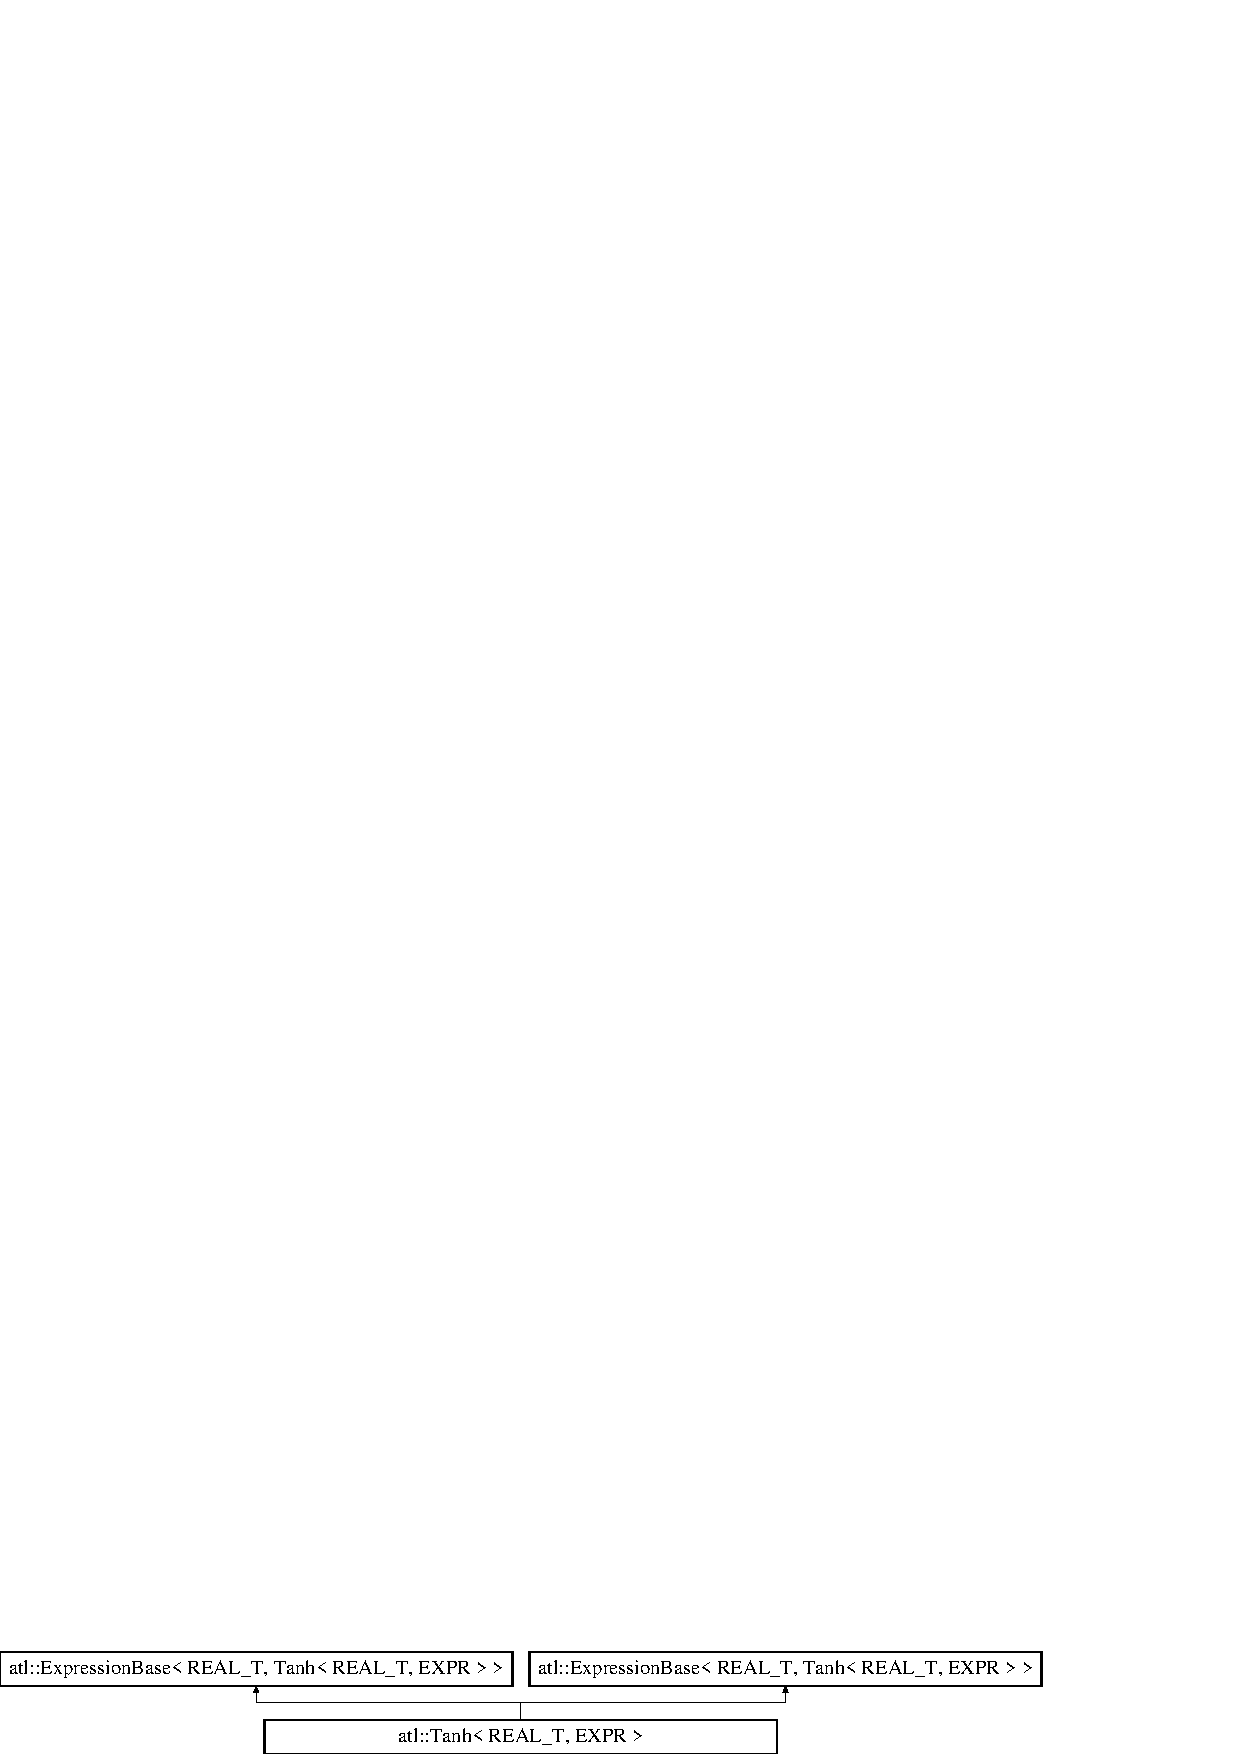
\includegraphics[height=1.609195cm]{structatl_1_1_tanh}
\end{center}
\end{figure}
\subsection*{Public Types}
\begin{DoxyCompactItemize}
\item 
\hypertarget{structatl_1_1_tanh_a02517badd82285f866990f93806f9812}{typedef R\+E\+A\+L\+\_\+\+T {\bfseries B\+A\+S\+E\+\_\+\+T\+Y\+P\+E}}\label{structatl_1_1_tanh_a02517badd82285f866990f93806f9812}

\item 
\hypertarget{structatl_1_1_tanh_a02517badd82285f866990f93806f9812}{typedef R\+E\+A\+L\+\_\+\+T {\bfseries B\+A\+S\+E\+\_\+\+T\+Y\+P\+E}}\label{structatl_1_1_tanh_a02517badd82285f866990f93806f9812}

\end{DoxyCompactItemize}
\subsection*{Public Member Functions}
\begin{DoxyCompactItemize}
\item 
\hypertarget{structatl_1_1_tanh_a653bd91c7ede867cdd382d463936cecd}{{\bfseries Tanh} (const \hyperlink{structatl_1_1_expression_base}{Expression\+Base}$<$ R\+E\+A\+L\+\_\+\+T, E\+X\+P\+R $>$ \&a)}\label{structatl_1_1_tanh_a653bd91c7ede867cdd382d463936cecd}

\item 
\hypertarget{structatl_1_1_tanh_af7853c511c4b0c2cb8f5ac8940f6a9bb}{const R\+E\+A\+L\+\_\+\+T {\bfseries Get\+Value} () const }\label{structatl_1_1_tanh_af7853c511c4b0c2cb8f5ac8940f6a9bb}

\item 
\hypertarget{structatl_1_1_tanh_a109ae48d7db65d57faeff76a2673e746}{const R\+E\+A\+L\+\_\+\+T {\bfseries Get\+Value} (size\+\_\+t i, size\+\_\+t j=0) const }\label{structatl_1_1_tanh_a109ae48d7db65d57faeff76a2673e746}

\item 
\hypertarget{structatl_1_1_tanh_a533181c192a4fa20640ae523586f76aa}{void {\bfseries Push\+Ids} (typename \hyperlink{structatl_1_1_stack_entry}{atl\+::\+Stack\+Entry}$<$ R\+E\+A\+L\+\_\+\+T $>$\+::vi\+\_\+storage \&ids) const }\label{structatl_1_1_tanh_a533181c192a4fa20640ae523586f76aa}

\item 
\hypertarget{structatl_1_1_tanh_ad42e0b192892e0541633e0444f8f2874}{void {\bfseries Push\+Ids} (typename \hyperlink{structatl_1_1_stack_entry}{atl\+::\+Stack\+Entry}$<$ R\+E\+A\+L\+\_\+\+T $>$\+::vi\+\_\+storage \&ids, size\+\_\+t i, size\+\_\+t j=0) const }\label{structatl_1_1_tanh_ad42e0b192892e0541633e0444f8f2874}

\item 
\hypertarget{structatl_1_1_tanh_af000d03c596d34baa208a3c4307c323f}{const R\+E\+A\+L\+\_\+\+T {\bfseries Evaluate\+Derivative} (uint32\+\_\+t id) const }\label{structatl_1_1_tanh_af000d03c596d34baa208a3c4307c323f}

\item 
\hypertarget{structatl_1_1_tanh_ac38515d4eac1331ab64d38bca7c46aa4}{R\+E\+A\+L\+\_\+\+T {\bfseries Evaluate\+Derivative} (uint32\+\_\+t a, uint32\+\_\+t b) const }\label{structatl_1_1_tanh_ac38515d4eac1331ab64d38bca7c46aa4}

\item 
\hypertarget{structatl_1_1_tanh_a1b74204c2742d5815cf15dbcde27f312}{R\+E\+A\+L\+\_\+\+T {\bfseries Evaluate\+Derivative} (uint32\+\_\+t x, uint32\+\_\+t y, uint32\+\_\+t z) const }\label{structatl_1_1_tanh_a1b74204c2742d5815cf15dbcde27f312}

\item 
\hypertarget{structatl_1_1_tanh_ae5ebf04ebc5b6d796ca6fdfd4c5507f0}{const R\+E\+A\+L\+\_\+\+T {\bfseries Evaluate\+Derivative} (uint32\+\_\+t id, size\+\_\+t i, size\+\_\+t j=0) const }\label{structatl_1_1_tanh_ae5ebf04ebc5b6d796ca6fdfd4c5507f0}

\item 
\hypertarget{structatl_1_1_tanh_abd23ed665740df232cf3913745b98a4e}{R\+E\+A\+L\+\_\+\+T {\bfseries Evaluate\+Derivative} (uint32\+\_\+t a, uint32\+\_\+t b, size\+\_\+t i, size\+\_\+t j=0) const }\label{structatl_1_1_tanh_abd23ed665740df232cf3913745b98a4e}

\item 
\hypertarget{structatl_1_1_tanh_aa18358c27e07440157ed6b3649d8c06b}{R\+E\+A\+L\+\_\+\+T {\bfseries Evaluate\+Derivative} (uint32\+\_\+t x, uint32\+\_\+t y, uint32\+\_\+t z, size\+\_\+t i, size\+\_\+t j=0) const }\label{structatl_1_1_tanh_aa18358c27e07440157ed6b3649d8c06b}

\item 
\hypertarget{structatl_1_1_tanh_a4516dfa2dc95b7bcfdda3289742814c6}{size\+\_\+t {\bfseries Get\+Columns} () const }\label{structatl_1_1_tanh_a4516dfa2dc95b7bcfdda3289742814c6}

\item 
\hypertarget{structatl_1_1_tanh_a7aada8d9c8678e5f0b763891cb16e854}{size\+\_\+t {\bfseries Get\+Rows} () const }\label{structatl_1_1_tanh_a7aada8d9c8678e5f0b763891cb16e854}

\item 
\hypertarget{structatl_1_1_tanh_a5beb83847e4cff2be39a4c4f82ee1ad7}{bool {\bfseries Is\+Scalar} () const }\label{structatl_1_1_tanh_a5beb83847e4cff2be39a4c4f82ee1ad7}

\item 
\hyperlink{structatl_1_1_tanh_a653bd91c7ede867cdd382d463936cecd}{Tanh} (const \hyperlink{structatl_1_1_expression_base}{Expression\+Base}$<$ R\+E\+A\+L\+\_\+\+T, E\+X\+P\+R $>$ \&a)
\item 
const R\+E\+A\+L\+\_\+\+T \hyperlink{structatl_1_1_tanh_af7853c511c4b0c2cb8f5ac8940f6a9bb}{Get\+Value} () const 
\item 
const R\+E\+A\+L\+\_\+\+T \hyperlink{structatl_1_1_tanh_a109ae48d7db65d57faeff76a2673e746}{Get\+Value} (size\+\_\+t i, size\+\_\+t j=0) const 
\item 
bool \hyperlink{structatl_1_1_tanh_aa2f425590c9ded0fabfa5d07c8235e41}{Is\+Nonlinear} () const 
\item 
void \hyperlink{structatl_1_1_tanh_a533181c192a4fa20640ae523586f76aa}{Push\+Ids} (typename \hyperlink{structatl_1_1_stack_entry}{atl\+::\+Stack\+Entry}$<$ R\+E\+A\+L\+\_\+\+T $>$\+::vi\+\_\+storage \&ids) const 
\item 
void \hyperlink{structatl_1_1_tanh_ad42e0b192892e0541633e0444f8f2874}{Push\+Ids} (typename \hyperlink{structatl_1_1_stack_entry}{atl\+::\+Stack\+Entry}$<$ R\+E\+A\+L\+\_\+\+T $>$\+::vi\+\_\+storage \&ids, size\+\_\+t i, size\+\_\+t j=0) const 
\item 
const R\+E\+A\+L\+\_\+\+T \hyperlink{structatl_1_1_tanh_a4564fcb43c3c39e01345fc9f1c2e2a10}{Evaluate\+Derivative} (uint32\+\_\+t x) const 
\item 
R\+E\+A\+L\+\_\+\+T \hyperlink{structatl_1_1_tanh_aeb4b49d9d17e12bc7fe34f2baba39e9d}{Evaluate\+Derivative} (uint32\+\_\+t x, uint32\+\_\+t y) const 
\item 
R\+E\+A\+L\+\_\+\+T \hyperlink{structatl_1_1_tanh_a1b74204c2742d5815cf15dbcde27f312}{Evaluate\+Derivative} (uint32\+\_\+t x, uint32\+\_\+t y, uint32\+\_\+t z) const 
\item 
const R\+E\+A\+L\+\_\+\+T \hyperlink{structatl_1_1_tanh_aa26a93417f964d20f6a93cbcda969bae}{Evaluate\+Derivative} (uint32\+\_\+t x, size\+\_\+t i, size\+\_\+t j=0) const 
\item 
R\+E\+A\+L\+\_\+\+T \hyperlink{structatl_1_1_tanh_a22bb2b84e980e041d8d2bd53e14867ed}{Evaluate\+Derivative} (uint32\+\_\+t x, uint32\+\_\+t y, size\+\_\+t i, size\+\_\+t j=0) const 
\item 
R\+E\+A\+L\+\_\+\+T \hyperlink{structatl_1_1_tanh_aa18358c27e07440157ed6b3649d8c06b}{Evaluate\+Derivative} (uint32\+\_\+t x, uint32\+\_\+t y, uint32\+\_\+t z, size\+\_\+t i, size\+\_\+t j=0) const 
\item 
size\+\_\+t \hyperlink{structatl_1_1_tanh_a7aada8d9c8678e5f0b763891cb16e854}{Get\+Rows} () const 
\item 
bool \hyperlink{structatl_1_1_tanh_a5beb83847e4cff2be39a4c4f82ee1ad7}{Is\+Scalar} () const 
\item 
const std\+::string \hyperlink{structatl_1_1_tanh_aa6cc749fc9a7b2087d2aed110bcf0871}{To\+Expression\+Template\+String} () const 
\end{DoxyCompactItemize}
\subsection*{Public Attributes}
\begin{DoxyCompactItemize}
\item 
\hypertarget{structatl_1_1_tanh_a8fe1ada69f03a3dd66c880dedf1cbdee}{const E\+X\+P\+R \& {\bfseries expr\+\_\+m}}\label{structatl_1_1_tanh_a8fe1ada69f03a3dd66c880dedf1cbdee}

\end{DoxyCompactItemize}


\subsection{Detailed Description}
\subsubsection*{template$<$class R\+E\+A\+L\+\_\+\+T, class E\+X\+P\+R$>$struct atl\+::\+Tanh$<$ R\+E\+A\+L\+\_\+\+T, E\+X\+P\+R $>$}

Expression template to handle hyperbolic tangent for variable or container expressions.

$ \tanh f(x) $

or

$ \tanh f_{i,j}(x) $ 

\subsection{Constructor \& Destructor Documentation}
\hypertarget{structatl_1_1_tanh_a653bd91c7ede867cdd382d463936cecd}{\index{atl\+::\+Tanh@{atl\+::\+Tanh}!Tanh@{Tanh}}
\index{Tanh@{Tanh}!atl\+::\+Tanh@{atl\+::\+Tanh}}
\subsubsection[{Tanh}]{\setlength{\rightskip}{0pt plus 5cm}template$<$class R\+E\+A\+L\+\_\+\+T , class E\+X\+P\+R $>$ {\bf atl\+::\+Tanh}$<$ R\+E\+A\+L\+\_\+\+T, E\+X\+P\+R $>$\+::{\bf Tanh} (
\begin{DoxyParamCaption}
\item[{const {\bf Expression\+Base}$<$ R\+E\+A\+L\+\_\+\+T, E\+X\+P\+R $>$ \&}]{a}
\end{DoxyParamCaption}
)\hspace{0.3cm}{\ttfamily [inline]}}}\label{structatl_1_1_tanh_a653bd91c7ede867cdd382d463936cecd}
Constructor.


\begin{DoxyParams}{Parameters}
{\em a} & \\
\hline
\end{DoxyParams}


\subsection{Member Function Documentation}
\hypertarget{structatl_1_1_tanh_a4564fcb43c3c39e01345fc9f1c2e2a10}{\index{atl\+::\+Tanh@{atl\+::\+Tanh}!Evaluate\+Derivative@{Evaluate\+Derivative}}
\index{Evaluate\+Derivative@{Evaluate\+Derivative}!atl\+::\+Tanh@{atl\+::\+Tanh}}
\subsubsection[{Evaluate\+Derivative}]{\setlength{\rightskip}{0pt plus 5cm}template$<$class R\+E\+A\+L\+\_\+\+T , class E\+X\+P\+R $>$ const R\+E\+A\+L\+\_\+\+T {\bf atl\+::\+Tanh}$<$ R\+E\+A\+L\+\_\+\+T, E\+X\+P\+R $>$\+::Evaluate\+Derivative (
\begin{DoxyParamCaption}
\item[{uint32\+\_\+t}]{x}
\end{DoxyParamCaption}
) const\hspace{0.3cm}{\ttfamily [inline]}}}\label{structatl_1_1_tanh_a4564fcb43c3c39e01345fc9f1c2e2a10}
Evaluates the first-\/order derivative with respect to x.

$ {\rm sech}\; ^2f(x)\,\left({{d}\over{d\,x}}\,f(x)\right) $


\begin{DoxyParams}{Parameters}
{\em x} & \\
\hline
\end{DoxyParams}
\begin{DoxyReturn}{Returns}

\end{DoxyReturn}
\hypertarget{structatl_1_1_tanh_aeb4b49d9d17e12bc7fe34f2baba39e9d}{\index{atl\+::\+Tanh@{atl\+::\+Tanh}!Evaluate\+Derivative@{Evaluate\+Derivative}}
\index{Evaluate\+Derivative@{Evaluate\+Derivative}!atl\+::\+Tanh@{atl\+::\+Tanh}}
\subsubsection[{Evaluate\+Derivative}]{\setlength{\rightskip}{0pt plus 5cm}template$<$class R\+E\+A\+L\+\_\+\+T , class E\+X\+P\+R $>$ R\+E\+A\+L\+\_\+\+T {\bf atl\+::\+Tanh}$<$ R\+E\+A\+L\+\_\+\+T, E\+X\+P\+R $>$\+::Evaluate\+Derivative (
\begin{DoxyParamCaption}
\item[{uint32\+\_\+t}]{x, }
\item[{uint32\+\_\+t}]{y}
\end{DoxyParamCaption}
) const\hspace{0.3cm}{\ttfamily [inline]}}}\label{structatl_1_1_tanh_aeb4b49d9d17e12bc7fe34f2baba39e9d}
Evaluates the second-\/order derivative with respect to x and y.

$ {\rm sech}\; ^2f(x,y)\,\left({{d^2}\over{d\,x\,d\,y}}\,f (x,y)\right)-2\,{\rm sech}\; ^2f(x,y)\,\tanh f(x,y)\, \left({{d}\over{d\,x}}\,f(x,y)\right)\,\left({{d}\over{d\,y}} \,f(x,y)\right) $


\begin{DoxyParams}{Parameters}
{\em x} & \\
\hline
{\em y} & \\
\hline
\end{DoxyParams}
\begin{DoxyReturn}{Returns}

\end{DoxyReturn}
\hypertarget{structatl_1_1_tanh_a1b74204c2742d5815cf15dbcde27f312}{\index{atl\+::\+Tanh@{atl\+::\+Tanh}!Evaluate\+Derivative@{Evaluate\+Derivative}}
\index{Evaluate\+Derivative@{Evaluate\+Derivative}!atl\+::\+Tanh@{atl\+::\+Tanh}}
\subsubsection[{Evaluate\+Derivative}]{\setlength{\rightskip}{0pt plus 5cm}template$<$class R\+E\+A\+L\+\_\+\+T , class E\+X\+P\+R $>$ R\+E\+A\+L\+\_\+\+T {\bf atl\+::\+Tanh}$<$ R\+E\+A\+L\+\_\+\+T, E\+X\+P\+R $>$\+::Evaluate\+Derivative (
\begin{DoxyParamCaption}
\item[{uint32\+\_\+t}]{x, }
\item[{uint32\+\_\+t}]{y, }
\item[{uint32\+\_\+t}]{z}
\end{DoxyParamCaption}
) const\hspace{0.3cm}{\ttfamily [inline]}}}\label{structatl_1_1_tanh_a1b74204c2742d5815cf15dbcde27f312}
Evaluates the third-\/order derivative with respect to x, y, z.

$ 4\,{\rm sech}\; ^2f(x,y,z)\,\tanh ^2f(x,y,z)\,\left({{d }\over{d\,x}}\,f(x,y,z)\right)\,\left({{d}\over{d\,y}}\,f (x,y,z)\right)\,\left({{d}\over{d\,z}}\,f(x,y,z)\right)- \\ 2\, {\rm sech}\; ^4f(x,y,z)\,\left({{d}\over{d\,x}}\,f(x,y,z )\right)\,\left({{d}\over{d\,y}}\,f(x,y,z)\right)\,\left({{d }\over{d\,z}}\,f(x,y,z)\right)- \\ 2\,{\rm sech}\; ^2f(x,y,z )\,\tanh f(x,y,z)\,\left({{d^2}\over{d\,x\,d\,y}}\,f(x,y ,z)\right)\,\left({{d}\over{d\,z}}\,f(x,y,z)\right)- \\ 2\, {\rm sech}\; ^2f(x,y,z)\,\tanh f(x,y,z)\,\left({{d }\over{d\,x}}\,f(x,y,z)\right)\,\left({{d^2}\over{d\,y\,d\,z}} \,f(x,y,z)\right)- \\ 2\,{\rm sech}\; ^2f(x,y,z)\,\tanh f(x,y,z)\, \left({{d^2}\over{d\,x\,d\,z}}\,f(x,y,z)\right)\, \left({{d}\over{d\,y}}\,f(x,y,z)\right)+ \\ {\rm sech}\; ^2f (x,y,z)\,\left({{d^3}\over{d\,x\,d\,y\,d\,z}}\,f(x,y,z)\right) $


\begin{DoxyParams}{Parameters}
{\em x} & \\
\hline
{\em y} & \\
\hline
{\em z} & \\
\hline
\end{DoxyParams}
\begin{DoxyReturn}{Returns}

\end{DoxyReturn}
\hypertarget{structatl_1_1_tanh_aa26a93417f964d20f6a93cbcda969bae}{\index{atl\+::\+Tanh@{atl\+::\+Tanh}!Evaluate\+Derivative@{Evaluate\+Derivative}}
\index{Evaluate\+Derivative@{Evaluate\+Derivative}!atl\+::\+Tanh@{atl\+::\+Tanh}}
\subsubsection[{Evaluate\+Derivative}]{\setlength{\rightskip}{0pt plus 5cm}template$<$class R\+E\+A\+L\+\_\+\+T , class E\+X\+P\+R $>$ const R\+E\+A\+L\+\_\+\+T {\bf atl\+::\+Tanh}$<$ R\+E\+A\+L\+\_\+\+T, E\+X\+P\+R $>$\+::Evaluate\+Derivative (
\begin{DoxyParamCaption}
\item[{uint32\+\_\+t}]{x, }
\item[{size\+\_\+t}]{i, }
\item[{size\+\_\+t}]{j = {\ttfamily 0}}
\end{DoxyParamCaption}
) const\hspace{0.3cm}{\ttfamily [inline]}}}\label{structatl_1_1_tanh_aa26a93417f964d20f6a93cbcda969bae}
Evaluates the first-\/order derivative with respect to x at index \{i,j\}.

$ {\rm sech}\; ^2f_{i,j}(x)\,\left({{d}\over{d\,x}}\,f_{i,j}(x) \right) $


\begin{DoxyParams}{Parameters}
{\em x} & \\
\hline
{\em i} & \\
\hline
{\em j} & \\
\hline
\end{DoxyParams}
\begin{DoxyReturn}{Returns}

\end{DoxyReturn}
\hypertarget{structatl_1_1_tanh_a22bb2b84e980e041d8d2bd53e14867ed}{\index{atl\+::\+Tanh@{atl\+::\+Tanh}!Evaluate\+Derivative@{Evaluate\+Derivative}}
\index{Evaluate\+Derivative@{Evaluate\+Derivative}!atl\+::\+Tanh@{atl\+::\+Tanh}}
\subsubsection[{Evaluate\+Derivative}]{\setlength{\rightskip}{0pt plus 5cm}template$<$class R\+E\+A\+L\+\_\+\+T , class E\+X\+P\+R $>$ R\+E\+A\+L\+\_\+\+T {\bf atl\+::\+Tanh}$<$ R\+E\+A\+L\+\_\+\+T, E\+X\+P\+R $>$\+::Evaluate\+Derivative (
\begin{DoxyParamCaption}
\item[{uint32\+\_\+t}]{x, }
\item[{uint32\+\_\+t}]{y, }
\item[{size\+\_\+t}]{i, }
\item[{size\+\_\+t}]{j = {\ttfamily 0}}
\end{DoxyParamCaption}
) const\hspace{0.3cm}{\ttfamily [inline]}}}\label{structatl_1_1_tanh_a22bb2b84e980e041d8d2bd53e14867ed}
Evaluates the second-\/order derivative with respect to x and y at index \{i,j\}.

$ {\rm sech}\; ^2f_{i,j}(x,y)\,\left({{d^2}\over{d\,x\,d\,y}}\,f_{i,j }(x,y)\right)-2\,{\rm sech}\; ^2f_{i,j}(x,y)\,\tanh f_{i,j}(x,y)\, \left({{d}\over{d\,x}}\,f_{i,j}(x,y)\right)\,\left({{d}\over{d\,y}} \,f_{i,j}(x,y)\right) $


\begin{DoxyParams}{Parameters}
{\em x} & \\
\hline
{\em y} & \\
\hline
{\em i} & \\
\hline
{\em j} & \\
\hline
\end{DoxyParams}
\begin{DoxyReturn}{Returns}

\end{DoxyReturn}
\hypertarget{structatl_1_1_tanh_aa18358c27e07440157ed6b3649d8c06b}{\index{atl\+::\+Tanh@{atl\+::\+Tanh}!Evaluate\+Derivative@{Evaluate\+Derivative}}
\index{Evaluate\+Derivative@{Evaluate\+Derivative}!atl\+::\+Tanh@{atl\+::\+Tanh}}
\subsubsection[{Evaluate\+Derivative}]{\setlength{\rightskip}{0pt plus 5cm}template$<$class R\+E\+A\+L\+\_\+\+T , class E\+X\+P\+R $>$ R\+E\+A\+L\+\_\+\+T {\bf atl\+::\+Tanh}$<$ R\+E\+A\+L\+\_\+\+T, E\+X\+P\+R $>$\+::Evaluate\+Derivative (
\begin{DoxyParamCaption}
\item[{uint32\+\_\+t}]{x, }
\item[{uint32\+\_\+t}]{y, }
\item[{uint32\+\_\+t}]{z, }
\item[{size\+\_\+t}]{i, }
\item[{size\+\_\+t}]{j = {\ttfamily 0}}
\end{DoxyParamCaption}
) const\hspace{0.3cm}{\ttfamily [inline]}}}\label{structatl_1_1_tanh_aa18358c27e07440157ed6b3649d8c06b}
Evaluates the third-\/order derivative with respect to x, y, z at index \{i,j\}.

$ 4\,{\rm sech}\; ^2f_{i,j}(x,y,z)\,\tanh ^2f_{i,j}(x,y,z)\,\left({{d }\over{d\,x}}\,f_{i,j}(x,y,z)\right)\,\left({{d}\over{d\,y}}\,f_{i,j }(x,y,z)\right)\,\left({{d}\over{d\,z}}\,f_{i,j}(x,y,z)\right)- \\ 2\, {\rm sech}\; ^4f_{i,j}(x,y,z)\,\left({{d}\over{d\,x}}\,f_{i,j}(x,y,z )\right)\,\left({{d}\over{d\,y}}\,f_{i,j}(x,y,z)\right)\,\left({{d }\over{d\,z}}\,f_{i,j}(x,y,z)\right)- \\ 2\,{\rm sech}\; ^2f_{i,j}(x,y,z )\,\tanh f_{i,j}(x,y,z)\,\left({{d^2}\over{d\,x\,d\,y}}\,f_{i,j}(x,y ,z)\right)\,\left({{d}\over{d\,z}}\,f_{i,j}(x,y,z)\right)- \\ 2\, {\rm sech}\; ^2f_{i,j}(x,y,z)\,\tanh f_{i,j}(x,y,z)\,\left({{d }\over{d\,x}}\,f_{i,j}(x,y,z)\right)\,\left({{d^2}\over{d\,y\,d\,z}} \,f_{i,j}(x,y,z)\right)- \\ 2\,{\rm sech}\; ^2f_{i,j}(x,y,z)\,\tanh f_{i ,j}(x,y,z)\,\left({{d^2}\over{d\,x\,d\,z}}\,f_{i,j}(x,y,z)\right)\, \left({{d}\over{d\,y}}\,f_{i,j}(x,y,z)\right)+ \\ {\rm sech}\; ^2f_{i,j} (x,y,z)\,\left({{d^3}\over{d\,x\,d\,y\,d\,z}}\,f_{i,j}(x,y,z)\right) $


\begin{DoxyParams}{Parameters}
{\em x} & \\
\hline
{\em y} & \\
\hline
{\em z} & \\
\hline
{\em i} & \\
\hline
{\em j} & \\
\hline
\end{DoxyParams}
\begin{DoxyReturn}{Returns}

\end{DoxyReturn}
\hypertarget{structatl_1_1_tanh_a7aada8d9c8678e5f0b763891cb16e854}{\index{atl\+::\+Tanh@{atl\+::\+Tanh}!Get\+Rows@{Get\+Rows}}
\index{Get\+Rows@{Get\+Rows}!atl\+::\+Tanh@{atl\+::\+Tanh}}
\subsubsection[{Get\+Rows}]{\setlength{\rightskip}{0pt plus 5cm}template$<$class R\+E\+A\+L\+\_\+\+T , class E\+X\+P\+R $>$ size\+\_\+t {\bf atl\+::\+Tanh}$<$ R\+E\+A\+L\+\_\+\+T, E\+X\+P\+R $>$\+::Get\+Rows (
\begin{DoxyParamCaption}
{}
\end{DoxyParamCaption}
) const\hspace{0.3cm}{\ttfamily [inline]}}}\label{structatl_1_1_tanh_a7aada8d9c8678e5f0b763891cb16e854}
Return the number of rows.

\begin{DoxyReturn}{Returns}

\end{DoxyReturn}
\hypertarget{structatl_1_1_tanh_af7853c511c4b0c2cb8f5ac8940f6a9bb}{\index{atl\+::\+Tanh@{atl\+::\+Tanh}!Get\+Value@{Get\+Value}}
\index{Get\+Value@{Get\+Value}!atl\+::\+Tanh@{atl\+::\+Tanh}}
\subsubsection[{Get\+Value}]{\setlength{\rightskip}{0pt plus 5cm}template$<$class R\+E\+A\+L\+\_\+\+T , class E\+X\+P\+R $>$ const R\+E\+A\+L\+\_\+\+T {\bf atl\+::\+Tanh}$<$ R\+E\+A\+L\+\_\+\+T, E\+X\+P\+R $>$\+::Get\+Value (
\begin{DoxyParamCaption}
{}
\end{DoxyParamCaption}
) const\hspace{0.3cm}{\ttfamily [inline]}}}\label{structatl_1_1_tanh_af7853c511c4b0c2cb8f5ac8940f6a9bb}
Computes the hyperbolic tangent of the evaluated expression.

\begin{DoxyReturn}{Returns}

\end{DoxyReturn}
\hypertarget{structatl_1_1_tanh_a109ae48d7db65d57faeff76a2673e746}{\index{atl\+::\+Tanh@{atl\+::\+Tanh}!Get\+Value@{Get\+Value}}
\index{Get\+Value@{Get\+Value}!atl\+::\+Tanh@{atl\+::\+Tanh}}
\subsubsection[{Get\+Value}]{\setlength{\rightskip}{0pt plus 5cm}template$<$class R\+E\+A\+L\+\_\+\+T , class E\+X\+P\+R $>$ const R\+E\+A\+L\+\_\+\+T {\bf atl\+::\+Tanh}$<$ R\+E\+A\+L\+\_\+\+T, E\+X\+P\+R $>$\+::Get\+Value (
\begin{DoxyParamCaption}
\item[{size\+\_\+t}]{i, }
\item[{size\+\_\+t}]{j = {\ttfamily 0}}
\end{DoxyParamCaption}
) const\hspace{0.3cm}{\ttfamily [inline]}}}\label{structatl_1_1_tanh_a109ae48d7db65d57faeff76a2673e746}
Computes the hyperbolic tangent of the evaluated expression at index \{i,j\}.

\begin{DoxyReturn}{Returns}

\end{DoxyReturn}
\hypertarget{structatl_1_1_tanh_aa2f425590c9ded0fabfa5d07c8235e41}{\index{atl\+::\+Tanh@{atl\+::\+Tanh}!Is\+Nonlinear@{Is\+Nonlinear}}
\index{Is\+Nonlinear@{Is\+Nonlinear}!atl\+::\+Tanh@{atl\+::\+Tanh}}
\subsubsection[{Is\+Nonlinear}]{\setlength{\rightskip}{0pt plus 5cm}template$<$class R\+E\+A\+L\+\_\+\+T , class E\+X\+P\+R $>$ bool {\bf atl\+::\+Tanh}$<$ R\+E\+A\+L\+\_\+\+T, E\+X\+P\+R $>$\+::Is\+Nonlinear (
\begin{DoxyParamCaption}
{}
\end{DoxyParamCaption}
) const\hspace{0.3cm}{\ttfamily [inline]}}}\label{structatl_1_1_tanh_aa2f425590c9ded0fabfa5d07c8235e41}
Returns true.

\begin{DoxyReturn}{Returns}

\end{DoxyReturn}
\hypertarget{structatl_1_1_tanh_a5beb83847e4cff2be39a4c4f82ee1ad7}{\index{atl\+::\+Tanh@{atl\+::\+Tanh}!Is\+Scalar@{Is\+Scalar}}
\index{Is\+Scalar@{Is\+Scalar}!atl\+::\+Tanh@{atl\+::\+Tanh}}
\subsubsection[{Is\+Scalar}]{\setlength{\rightskip}{0pt plus 5cm}template$<$class R\+E\+A\+L\+\_\+\+T , class E\+X\+P\+R $>$ bool {\bf atl\+::\+Tanh}$<$ R\+E\+A\+L\+\_\+\+T, E\+X\+P\+R $>$\+::Is\+Scalar (
\begin{DoxyParamCaption}
{}
\end{DoxyParamCaption}
) const\hspace{0.3cm}{\ttfamily [inline]}}}\label{structatl_1_1_tanh_a5beb83847e4cff2be39a4c4f82ee1ad7}
True if this expression is a scalar.

\begin{DoxyReturn}{Returns}

\end{DoxyReturn}
\hypertarget{structatl_1_1_tanh_a533181c192a4fa20640ae523586f76aa}{\index{atl\+::\+Tanh@{atl\+::\+Tanh}!Push\+Ids@{Push\+Ids}}
\index{Push\+Ids@{Push\+Ids}!atl\+::\+Tanh@{atl\+::\+Tanh}}
\subsubsection[{Push\+Ids}]{\setlength{\rightskip}{0pt plus 5cm}template$<$class R\+E\+A\+L\+\_\+\+T , class E\+X\+P\+R $>$ void {\bf atl\+::\+Tanh}$<$ R\+E\+A\+L\+\_\+\+T, E\+X\+P\+R $>$\+::Push\+Ids (
\begin{DoxyParamCaption}
\item[{typename {\bf atl\+::\+Stack\+Entry}$<$ R\+E\+A\+L\+\_\+\+T $>$\+::vi\+\_\+storage \&}]{ids}
\end{DoxyParamCaption}
) const\hspace{0.3cm}{\ttfamily [inline]}}}\label{structatl_1_1_tanh_a533181c192a4fa20640ae523586f76aa}
Push variable info into a set.


\begin{DoxyParams}{Parameters}
{\em ids} & \\
\hline
\end{DoxyParams}
\hypertarget{structatl_1_1_tanh_ad42e0b192892e0541633e0444f8f2874}{\index{atl\+::\+Tanh@{atl\+::\+Tanh}!Push\+Ids@{Push\+Ids}}
\index{Push\+Ids@{Push\+Ids}!atl\+::\+Tanh@{atl\+::\+Tanh}}
\subsubsection[{Push\+Ids}]{\setlength{\rightskip}{0pt plus 5cm}template$<$class R\+E\+A\+L\+\_\+\+T , class E\+X\+P\+R $>$ void {\bf atl\+::\+Tanh}$<$ R\+E\+A\+L\+\_\+\+T, E\+X\+P\+R $>$\+::Push\+Ids (
\begin{DoxyParamCaption}
\item[{typename {\bf atl\+::\+Stack\+Entry}$<$ R\+E\+A\+L\+\_\+\+T $>$\+::vi\+\_\+storage \&}]{ids, }
\item[{size\+\_\+t}]{i, }
\item[{size\+\_\+t}]{j = {\ttfamily 0}}
\end{DoxyParamCaption}
) const\hspace{0.3cm}{\ttfamily [inline]}}}\label{structatl_1_1_tanh_ad42e0b192892e0541633e0444f8f2874}
Push variable info into a set at index \{i,j\}.


\begin{DoxyParams}{Parameters}
{\em ids} & \\
\hline
{\em i} & \\
\hline
{\em j} & \\
\hline
\end{DoxyParams}
\hypertarget{structatl_1_1_tanh_aa6cc749fc9a7b2087d2aed110bcf0871}{\index{atl\+::\+Tanh@{atl\+::\+Tanh}!To\+Expression\+Template\+String@{To\+Expression\+Template\+String}}
\index{To\+Expression\+Template\+String@{To\+Expression\+Template\+String}!atl\+::\+Tanh@{atl\+::\+Tanh}}
\subsubsection[{To\+Expression\+Template\+String}]{\setlength{\rightskip}{0pt plus 5cm}template$<$class R\+E\+A\+L\+\_\+\+T , class E\+X\+P\+R $>$ const std\+::string {\bf atl\+::\+Tanh}$<$ R\+E\+A\+L\+\_\+\+T, E\+X\+P\+R $>$\+::To\+Expression\+Template\+String (
\begin{DoxyParamCaption}
{}
\end{DoxyParamCaption}
) const\hspace{0.3cm}{\ttfamily [inline]}}}\label{structatl_1_1_tanh_aa6cc749fc9a7b2087d2aed110bcf0871}
Create a string representation of this expression template. \begin{DoxyReturn}{Returns}

\end{DoxyReturn}


The documentation for this struct was generated from the following file\+:\begin{DoxyCompactItemize}
\item 
A\+T\+L2/Tanh.\+hpp\end{DoxyCompactItemize}

\hypertarget{classatl_1_1_tape}{\section{atl\+:\+:Tape$<$ R\+E\+A\+L\+\_\+\+T $>$ Class Template Reference}
\label{classatl_1_1_tape}\index{atl\+::\+Tape$<$ R\+E\+A\+L\+\_\+\+T $>$@{atl\+::\+Tape$<$ R\+E\+A\+L\+\_\+\+T $>$}}
}


{\ttfamily \#include $<$Tape.\+hpp$>$}

\subsection*{Public Member Functions}
\begin{DoxyCompactItemize}
\item 
\hypertarget{classatl_1_1_tape_ab5c9657e3efac59a8ff196af2ec2850d}{{\bfseries Tape} (size\+\_\+t size=100000)}\label{classatl_1_1_tape_ab5c9657e3efac59a8ff196af2ec2850d}

\item 
\hypertarget{classatl_1_1_tape_aae53cfc50b4b2901f400d61d493b3d89}{size\+\_\+t {\bfseries Get\+Block} (size\+\_\+t size)}\label{classatl_1_1_tape_aae53cfc50b4b2901f400d61d493b3d89}

\item 
const size\+\_\+t \hyperlink{classatl_1_1_tape_a62931ab955573c27faa83056959add48}{Next\+Index} ()
\item 
\hypertarget{classatl_1_1_tape_a5466d55b5e2f3a463bbbe6521cf49359}{void {\bfseries Accumulate} ()}\label{classatl_1_1_tape_a5466d55b5e2f3a463bbbe6521cf49359}

\item 
\hyperlink{classatl_1_1_tape_a6ea5c0894ee230b8f7217743317c2519}{Tape} (size\+\_\+t size=10000000)
\item 
size\+\_\+t \hyperlink{classatl_1_1_tape_aae53cfc50b4b2901f400d61d493b3d89}{Get\+Block} (size\+\_\+t size)
\item 
const size\+\_\+t \hyperlink{classatl_1_1_tape_a62931ab955573c27faa83056959add48}{Next\+Index} ()
\item 
\hypertarget{classatl_1_1_tape_aad99808e9f19174a397eac6c26f092bb}{R\+E\+A\+L\+\_\+\+T \& {\bfseries Reference} (uint32\+\_\+t i)}\label{classatl_1_1_tape_aad99808e9f19174a397eac6c26f092bb}

\item 
\hypertarget{classatl_1_1_tape_a540945c7ce2e849eb6e748b12d317a61}{R\+E\+A\+L\+\_\+\+T \& {\bfseries Reference} (uint32\+\_\+t i, uint32\+\_\+t j)}\label{classatl_1_1_tape_a540945c7ce2e849eb6e748b12d317a61}

\item 
\hypertarget{classatl_1_1_tape_a507c33a9c2f85a5229042bc635699e44}{R\+E\+A\+L\+\_\+\+T \& {\bfseries Reference} (uint32\+\_\+t i, uint32\+\_\+t j, uint32\+\_\+t k)}\label{classatl_1_1_tape_a507c33a9c2f85a5229042bc635699e44}

\item 
\hypertarget{classatl_1_1_tape_a69f08d0d927e3be29969cfada0b498d5}{const R\+E\+A\+L\+\_\+\+T {\bfseries Value} (uint32\+\_\+t i)}\label{classatl_1_1_tape_a69f08d0d927e3be29969cfada0b498d5}

\item 
\hypertarget{classatl_1_1_tape_a362fe066cd6b4ae9ddfde320feebc206}{const R\+E\+A\+L\+\_\+\+T {\bfseries Value} (uint32\+\_\+t i, uint32\+\_\+t j)}\label{classatl_1_1_tape_a362fe066cd6b4ae9ddfde320feebc206}

\item 
\hypertarget{classatl_1_1_tape_a8e16f61e76688105fb8aeb25ebfbeeaf}{const R\+E\+A\+L\+\_\+\+T {\bfseries Value} (uint32\+\_\+t i, uint32\+\_\+t j, uint32\+\_\+t k)}\label{classatl_1_1_tape_a8e16f61e76688105fb8aeb25ebfbeeaf}

\item 
void \hyperlink{classatl_1_1_tape_a5466d55b5e2f3a463bbbe6521cf49359}{Accumulate} ()
\item 
\hypertarget{classatl_1_1_tape_af0d63ed0c151614290bae44e5d7b07cb}{void {\bfseries Accumulate\+First\+Order} ()}\label{classatl_1_1_tape_af0d63ed0c151614290bae44e5d7b07cb}

\item 
\hypertarget{classatl_1_1_tape_a9d12d59ac03929ec8a5d05d14bad9a68}{void {\bfseries Accumulate\+Second\+Order} ()}\label{classatl_1_1_tape_a9d12d59ac03929ec8a5d05d14bad9a68}

\item 
\hypertarget{classatl_1_1_tape_a2aece965b7b72ee6a9b7789da7c41006}{void {\bfseries Accumulate\+Third\+Order} ()}\label{classatl_1_1_tape_a2aece965b7b72ee6a9b7789da7c41006}

\end{DoxyCompactItemize}
\subsection*{Public Attributes}
\begin{DoxyCompactItemize}
\item 
\hypertarget{classatl_1_1_tape_a50fafd1ce08712228c92f4ca38440151}{std\+::unordered\+\_\+map$<$ uint32\+\_\+t, \\*
R\+E\+A\+L\+\_\+\+T $>$ {\bfseries first\+\_\+order\+\_\+derivtives}}\label{classatl_1_1_tape_a50fafd1ce08712228c92f4ca38440151}

\item 
\hypertarget{classatl_1_1_tape_af9f09277d29a4a1324a654b8941939c0}{std\+::vector$<$ \hyperlink{structatl_1_1_stack_entry}{Stack\+Entry}\\*
$<$ R\+E\+A\+L\+\_\+\+T $>$, \hyperlink{structatl_1_1clfallocator}{atl\+::clfallocator}\\*
$<$ \hyperlink{structatl_1_1_stack_entry}{Stack\+Entry}$<$ R\+E\+A\+L\+\_\+\+T $>$ $>$ $>$ {\bfseries stack}}\label{classatl_1_1_tape_af9f09277d29a4a1324a654b8941939c0}

\item 
\hypertarget{classatl_1_1_tape_a1865935ec7575eef6cb103422ea90a11}{std\+::atomic$<$ size\+\_\+t $>$ {\bfseries stack\+\_\+current}}\label{classatl_1_1_tape_a1865935ec7575eef6cb103422ea90a11}

\item 
\hypertarget{classatl_1_1_tape_a4687370d86d77a34775056f2ee4eb267}{bool {\bfseries recording} = true}\label{classatl_1_1_tape_a4687370d86d77a34775056f2ee4eb267}

\item 
\hypertarget{classatl_1_1_tape_a03b20777c410ed3e24d3d62a9deee7be}{Derivative\+Trace\+Level {\bfseries derivative\+\_\+trace\+\_\+level} = F\+I\+R\+S\+T\+\_\+\+O\+R\+D\+E\+R\+\_\+\+R\+E\+V\+E\+R\+S\+E}\label{classatl_1_1_tape_a03b20777c410ed3e24d3d62a9deee7be}

\item 
\hypertarget{classatl_1_1_tape_ac6ae094e22186a5b8c8084b962a0639e}{first\+\_\+order\+\_\+container {\bfseries first\+\_\+order\+\_\+derivatives}}\label{classatl_1_1_tape_ac6ae094e22186a5b8c8084b962a0639e}

\item 
\hypertarget{classatl_1_1_tape_a8ba1395fef83806c8a5ce69919185e51}{second\+\_\+order\+\_\+container {\bfseries second\+\_\+order\+\_\+derivatives}}\label{classatl_1_1_tape_a8ba1395fef83806c8a5ce69919185e51}

\item 
\hypertarget{classatl_1_1_tape_abd4860921248ac2178291a35451df33e}{third\+\_\+order\+\_\+container {\bfseries third\+\_\+order\+\_\+derivatives}}\label{classatl_1_1_tape_abd4860921248ac2178291a35451df33e}

\item 
\hypertarget{classatl_1_1_tape_a052ab59b9967c0a85408b489a4975f22}{std\+::unordered\+\_\+map$<$ uint32\+\_\+t, \\*
\hyperlink{structatl_1_1_forward_mode_derivative_info}{Forward\+Mode\+Derivative\+Info}\\*
$<$ R\+E\+A\+L\+\_\+\+T $>$ $>$ {\bfseries forward\+\_\+mode\+\_\+derivative\+\_\+info}}\label{classatl_1_1_tape_a052ab59b9967c0a85408b489a4975f22}

\end{DoxyCompactItemize}


\subsection{Detailed Description}
\subsubsection*{template$<$typename R\+E\+A\+L\+\_\+\+T$>$class atl\+::\+Tape$<$ R\+E\+A\+L\+\_\+\+T $>$}

\hyperlink{classatl_1_1_tape}{Tape} class for recording adjoint derivative information that will be used in reverse mode accumulation upt to third-\/order. 

\subsection{Constructor \& Destructor Documentation}
\hypertarget{classatl_1_1_tape_a6ea5c0894ee230b8f7217743317c2519}{\index{atl\+::\+Tape@{atl\+::\+Tape}!Tape@{Tape}}
\index{Tape@{Tape}!atl\+::\+Tape@{atl\+::\+Tape}}
\subsubsection[{Tape}]{\setlength{\rightskip}{0pt plus 5cm}template$<$typename R\+E\+A\+L\+\_\+\+T$>$ {\bf atl\+::\+Tape}$<$ R\+E\+A\+L\+\_\+\+T $>$\+::{\bf Tape} (
\begin{DoxyParamCaption}
\item[{size\+\_\+t}]{size = {\ttfamily 10000000}}
\end{DoxyParamCaption}
)\hspace{0.3cm}{\ttfamily [inline]}}}\label{classatl_1_1_tape_a6ea5c0894ee230b8f7217743317c2519}
Constructor.

Reserves memory for the tape to {\itshape size}.


\begin{DoxyParams}{Parameters}
{\em size} & \\
\hline
\end{DoxyParams}


\subsection{Member Function Documentation}
\hypertarget{classatl_1_1_tape_a5466d55b5e2f3a463bbbe6521cf49359}{\index{atl\+::\+Tape@{atl\+::\+Tape}!Accumulate@{Accumulate}}
\index{Accumulate@{Accumulate}!atl\+::\+Tape@{atl\+::\+Tape}}
\subsubsection[{Accumulate}]{\setlength{\rightskip}{0pt plus 5cm}template$<$typename R\+E\+A\+L\+\_\+\+T$>$ void {\bf atl\+::\+Tape}$<$ R\+E\+A\+L\+\_\+\+T $>$\+::Accumulate (
\begin{DoxyParamCaption}
{}
\end{DoxyParamCaption}
)\hspace{0.3cm}{\ttfamily [inline]}}}\label{classatl_1_1_tape_a5466d55b5e2f3a463bbbe6521cf49359}
Accumulates reverse mode derivatives according to {\itshape derivative\+\_\+trace\+\_\+level}. \hypertarget{classatl_1_1_tape_aae53cfc50b4b2901f400d61d493b3d89}{\index{atl\+::\+Tape@{atl\+::\+Tape}!Get\+Block@{Get\+Block}}
\index{Get\+Block@{Get\+Block}!atl\+::\+Tape@{atl\+::\+Tape}}
\subsubsection[{Get\+Block}]{\setlength{\rightskip}{0pt plus 5cm}template$<$typename R\+E\+A\+L\+\_\+\+T$>$ size\+\_\+t {\bf atl\+::\+Tape}$<$ R\+E\+A\+L\+\_\+\+T $>$\+::Get\+Block (
\begin{DoxyParamCaption}
\item[{size\+\_\+t}]{size}
\end{DoxyParamCaption}
)\hspace{0.3cm}{\ttfamily [inline]}}}\label{classatl_1_1_tape_aae53cfc50b4b2901f400d61d493b3d89}
Atomic operation.

Allocates a block of tape entries. Adds {\itshape size} to the {\itshape stack\+\_\+current} member. Useful for concurrent container operations.


\begin{DoxyParams}{Parameters}
{\em size} & \\
\hline
\end{DoxyParams}
\begin{DoxyReturn}{Returns}

\end{DoxyReturn}
\hypertarget{classatl_1_1_tape_a62931ab955573c27faa83056959add48}{\index{atl\+::\+Tape@{atl\+::\+Tape}!Next\+Index@{Next\+Index}}
\index{Next\+Index@{Next\+Index}!atl\+::\+Tape@{atl\+::\+Tape}}
\subsubsection[{Next\+Index}]{\setlength{\rightskip}{0pt plus 5cm}template$<$typename R\+E\+A\+L\+\_\+\+T$>$ const size\+\_\+t {\bf atl\+::\+Tape}$<$ R\+E\+A\+L\+\_\+\+T $>$\+::Next\+Index (
\begin{DoxyParamCaption}
{}
\end{DoxyParamCaption}
)\hspace{0.3cm}{\ttfamily [inline]}}}\label{classatl_1_1_tape_a62931ab955573c27faa83056959add48}
Atomic operation. Gets the next available index in the stack.

\begin{DoxyReturn}{Returns}

\end{DoxyReturn}


Referenced by atl\+::\+Variable$<$ T $>$\+::\+Assign().

\hypertarget{classatl_1_1_tape_a62931ab955573c27faa83056959add48}{\index{atl\+::\+Tape@{atl\+::\+Tape}!Next\+Index@{Next\+Index}}
\index{Next\+Index@{Next\+Index}!atl\+::\+Tape@{atl\+::\+Tape}}
\subsubsection[{Next\+Index}]{\setlength{\rightskip}{0pt plus 5cm}template$<$typename R\+E\+A\+L\+\_\+\+T$>$ const size\+\_\+t {\bf atl\+::\+Tape}$<$ R\+E\+A\+L\+\_\+\+T $>$\+::Next\+Index (
\begin{DoxyParamCaption}
{}
\end{DoxyParamCaption}
)\hspace{0.3cm}{\ttfamily [inline]}}}\label{classatl_1_1_tape_a62931ab955573c27faa83056959add48}
Atomic operation. Gets the next available index in the stack.

\begin{DoxyReturn}{Returns}

\end{DoxyReturn}


The documentation for this class was generated from the following file\+:\begin{DoxyCompactItemize}
\item 
A\+T\+L2/Tape.\+hpp\end{DoxyCompactItemize}

\hypertarget{struct_thread_function}{\section{Thread\+Function Struct Reference}
\label{struct_thread_function}\index{Thread\+Function@{Thread\+Function}}
}
\subsection*{Public Member Functions}
\begin{DoxyCompactItemize}
\item 
\hypertarget{struct_thread_function_a0c805c4816d400a48e130c7678781864}{{\bfseries Thread\+Function} (int start, int end, std\+::vector$<$ \hyperlink{structatl_1_1_variable}{atl\+::\+Variable}$<$ double $>$ $>$ \&v, \hyperlink{structatl_1_1_variable}{atl\+::\+Variable}$<$ double $>$ \&m, int estart)}\label{struct_thread_function_a0c805c4816d400a48e130c7678781864}

\item 
\hypertarget{struct_thread_function_aba725fb009acea384e8bbc7dda37e1ac}{void {\bfseries operator()} ()}\label{struct_thread_function_aba725fb009acea384e8bbc7dda37e1ac}

\end{DoxyCompactItemize}
\subsection*{Public Attributes}
\begin{DoxyCompactItemize}
\item 
\hypertarget{struct_thread_function_ac325eb85204edea0589a0ec74c5031e6}{int {\bfseries start}}\label{struct_thread_function_ac325eb85204edea0589a0ec74c5031e6}

\item 
\hypertarget{struct_thread_function_a1156a7146122601aa9fadb69a128de3b}{int {\bfseries end}}\label{struct_thread_function_a1156a7146122601aa9fadb69a128de3b}

\item 
\hypertarget{struct_thread_function_a4be77062174107b85dc9abd350d56a1b}{std\+::vector$<$ \hyperlink{structatl_1_1_variable}{atl\+::\+Variable}\\*
$<$ double $>$ $>$ \& {\bfseries v}}\label{struct_thread_function_a4be77062174107b85dc9abd350d56a1b}

\item 
\hypertarget{struct_thread_function_a79b606f5addb749a99b0b01e63179383}{\hyperlink{structatl_1_1_variable}{atl\+::\+Variable}$<$ double $>$ \& {\bfseries maxv}}\label{struct_thread_function_a79b606f5addb749a99b0b01e63179383}

\item 
\hypertarget{struct_thread_function_adc46ddcc785ec62c6a458d80a486eb8a}{int {\bfseries estart}}\label{struct_thread_function_adc46ddcc785ec62c6a458d80a486eb8a}

\end{DoxyCompactItemize}


\subsection{Detailed Description}
Returns the minimum between a and b in a continuous manner using\+:

(a + b -\/ $\vert$a.Get\+Value() -\/ b.\+Get\+Value()$\vert$) / 2.\+0;


\begin{DoxyParams}{Parameters}
{\em a} & \\
\hline
{\em b} & \\
\hline
\end{DoxyParams}
\begin{DoxyReturn}{Returns}

\end{DoxyReturn}


The documentation for this struct was generated from the following file\+:\begin{DoxyCompactItemize}
\item 
main.\+cpp\end{DoxyCompactItemize}

\hypertarget{classatl_1_1_thread_pool}{\section{atl\+:\+:Thread\+Pool Class Reference}
\label{classatl_1_1_thread_pool}\index{atl\+::\+Thread\+Pool@{atl\+::\+Thread\+Pool}}
}


{\ttfamily \#include $<$Thread\+Pool.\+hpp$>$}

\subsection*{Public Member Functions}
\begin{DoxyCompactItemize}
\item 
\hypertarget{classatl_1_1_thread_pool_a02ca8a74131b65469a77d09637971865}{{\bfseries Thread\+Pool} (int threads=std\+::thread\+::hardware\+\_\+concurrency())}\label{classatl_1_1_thread_pool_a02ca8a74131b65469a77d09637971865}

\item 
\hypertarget{classatl_1_1_thread_pool_a96599097f0e7ac0665b16ea23cd5d014}{void {\bfseries Start} (int threads=std\+::thread\+::hardware\+\_\+concurrency())}\label{classatl_1_1_thread_pool_a96599097f0e7ac0665b16ea23cd5d014}

\item 
\hypertarget{classatl_1_1_thread_pool_afaaedabb66c24d2dffadad1a17ee326e}{size\+\_\+t {\bfseries Size} ()}\label{classatl_1_1_thread_pool_afaaedabb66c24d2dffadad1a17ee326e}

\item 
\hypertarget{classatl_1_1_thread_pool_a98a69f6bc963f87dcde08db1f30a24c8}{void {\bfseries Do\+Job} (std\+::function$<$ void(void) $>$ func)}\label{classatl_1_1_thread_pool_a98a69f6bc963f87dcde08db1f30a24c8}

\item 
\hypertarget{classatl_1_1_thread_pool_ab11df304a64fb8d887f4fe2ef7fc66f9}{void {\bfseries Do\+Job} (std\+::function$<$ void(void) $>$ func, \hyperlink{classatl_1_1_wait_variable}{Wait\+Variable} \&wait)}\label{classatl_1_1_thread_pool_ab11df304a64fb8d887f4fe2ef7fc66f9}

\item 
\hypertarget{classatl_1_1_thread_pool_a6096504a6d4a74ec14ca8235ab9615b5}{{\footnotesize template$<$class Input\+It , typename Function $>$ }\\void {\bfseries For\+Each} (Input\+It first, const size\+\_\+t \&elements, const Function \&function)}\label{classatl_1_1_thread_pool_a6096504a6d4a74ec14ca8235ab9615b5}

\item 
\hypertarget{classatl_1_1_thread_pool_a16ebafa211b0c60aa56fc839a646a758}{{\footnotesize template$<$class Input\+It , typename Function $>$ }\\void {\bfseries For\+Each} (Input\+It first, const size\+\_\+t \&elements, const Function \&function, \hyperlink{classatl_1_1_wait_variable}{Wait\+Variable} \&wait)}\label{classatl_1_1_thread_pool_a16ebafa211b0c60aa56fc839a646a758}

\item 
\hypertarget{classatl_1_1_thread_pool_a59f8f9c30945196c845ee26c1d1dfd10}{void {\bfseries Wait} (\hyperlink{classatl_1_1_wait_variable}{Wait\+Variable} \&wait)}\label{classatl_1_1_thread_pool_a59f8f9c30945196c845ee26c1d1dfd10}

\item 
\hyperlink{classatl_1_1_thread_pool_a02ca8a74131b65469a77d09637971865}{Thread\+Pool} (int threads=std\+::thread\+::hardware\+\_\+concurrency())
\item 
\hyperlink{classatl_1_1_thread_pool_a487944b9f55c77a0d74ebc9f129e1ad3}{$\sim$\+Thread\+Pool} ()
\item 
\hypertarget{classatl_1_1_thread_pool_a96599097f0e7ac0665b16ea23cd5d014}{void {\bfseries Start} (int threads=std\+::thread\+::hardware\+\_\+concurrency())}\label{classatl_1_1_thread_pool_a96599097f0e7ac0665b16ea23cd5d014}

\item 
size\+\_\+t \hyperlink{classatl_1_1_thread_pool_afaaedabb66c24d2dffadad1a17ee326e}{Size} ()
\item 
void \hyperlink{classatl_1_1_thread_pool_a98a69f6bc963f87dcde08db1f30a24c8}{Do\+Job} (std\+::function$<$ void(void) $>$ func)
\item 
void \hyperlink{classatl_1_1_thread_pool_ab11df304a64fb8d887f4fe2ef7fc66f9}{Do\+Job} (std\+::function$<$ void(void) $>$ func, \hyperlink{classatl_1_1_wait_variable}{Wait\+Variable} \&wait)
\item 
{\footnotesize template$<$class Input\+It , typename Function $>$ }\\void \hyperlink{classatl_1_1_thread_pool_a6096504a6d4a74ec14ca8235ab9615b5}{For\+Each} (Input\+It first, const size\+\_\+t \&elements, const Function \&function)
\item 
{\footnotesize template$<$class Input\+It , typename Function $>$ }\\void \hyperlink{classatl_1_1_thread_pool_a16ebafa211b0c60aa56fc839a646a758}{For\+Each} (Input\+It first, const size\+\_\+t \&elements, const Function \&function, \hyperlink{classatl_1_1_wait_variable}{Wait\+Variable} \&wait)
\item 
void \hyperlink{classatl_1_1_thread_pool_a59f8f9c30945196c845ee26c1d1dfd10}{Wait} (\hyperlink{classatl_1_1_wait_variable}{Wait\+Variable} \&wait)
\end{DoxyCompactItemize}
\subsection*{Protected Member Functions}
\begin{DoxyCompactItemize}
\item 
\hypertarget{classatl_1_1_thread_pool_ab442364a73d9184b4f0adfd3f47ea2fb}{void {\bfseries thread\+Entry} (int i)}\label{classatl_1_1_thread_pool_ab442364a73d9184b4f0adfd3f47ea2fb}

\item 
\hypertarget{classatl_1_1_thread_pool_ab442364a73d9184b4f0adfd3f47ea2fb}{void {\bfseries thread\+Entry} (int i)}\label{classatl_1_1_thread_pool_ab442364a73d9184b4f0adfd3f47ea2fb}

\end{DoxyCompactItemize}
\subsection*{Protected Attributes}
\begin{DoxyCompactItemize}
\item 
\hypertarget{classatl_1_1_thread_pool_a402283160a126b60093c4304f3007458}{std\+::mutex {\bfseries lock\+\_\+}}\label{classatl_1_1_thread_pool_a402283160a126b60093c4304f3007458}

\item 
\hypertarget{classatl_1_1_thread_pool_a4e5d8a799ea40e346a83d5877ae67cbb}{std\+::condition\+\_\+variable {\bfseries cond\+Var\+\_\+}}\label{classatl_1_1_thread_pool_a4e5d8a799ea40e346a83d5877ae67cbb}

\item 
\hypertarget{classatl_1_1_thread_pool_a44df4799943e50ea24f1a036ff3db2f6}{bool {\bfseries shutdown\+\_\+}}\label{classatl_1_1_thread_pool_a44df4799943e50ea24f1a036ff3db2f6}

\item 
\hypertarget{classatl_1_1_thread_pool_a44aba02e981bdb14f52f8ef364b0cc65}{bool {\bfseries started\+\_\+}}\label{classatl_1_1_thread_pool_a44aba02e981bdb14f52f8ef364b0cc65}

\item 
\hypertarget{classatl_1_1_thread_pool_a783028a9da8da6892c76667b163f084e}{size\+\_\+t {\bfseries thread\+\_\+count}}\label{classatl_1_1_thread_pool_a783028a9da8da6892c76667b163f084e}

\item 
\hypertarget{classatl_1_1_thread_pool_af27763f5a3533a7280ffbb929864081e}{std\+::queue$<$ std\+::function\\*
$<$ void(void) $>$ $>$ {\bfseries jobs\+\_\+}}\label{classatl_1_1_thread_pool_af27763f5a3533a7280ffbb929864081e}

\item 
\hypertarget{classatl_1_1_thread_pool_a15e4c898954139d882304533e7b245d4}{std\+::vector$<$ std\+::thread $>$ {\bfseries threads\+\_\+}}\label{classatl_1_1_thread_pool_a15e4c898954139d882304533e7b245d4}

\end{DoxyCompactItemize}


\subsection{Detailed Description}
Thread pool. 

\subsection{Constructor \& Destructor Documentation}
\hypertarget{classatl_1_1_thread_pool_a02ca8a74131b65469a77d09637971865}{\index{atl\+::\+Thread\+Pool@{atl\+::\+Thread\+Pool}!Thread\+Pool@{Thread\+Pool}}
\index{Thread\+Pool@{Thread\+Pool}!atl\+::\+Thread\+Pool@{atl\+::\+Thread\+Pool}}
\subsubsection[{Thread\+Pool}]{\setlength{\rightskip}{0pt plus 5cm}atl\+::\+Thread\+Pool\+::\+Thread\+Pool (
\begin{DoxyParamCaption}
\item[{int}]{threads = {\ttfamily std\+:\+:thread\+:\+:hardware\+\_\+concurrency()}}
\end{DoxyParamCaption}
)\hspace{0.3cm}{\ttfamily [inline]}}}\label{classatl_1_1_thread_pool_a02ca8a74131b65469a77d09637971865}
Constructor. Sets the number of threads in this thread pool.


\begin{DoxyParams}{Parameters}
{\em threads} & \\
\hline
\end{DoxyParams}
\hypertarget{classatl_1_1_thread_pool_a487944b9f55c77a0d74ebc9f129e1ad3}{\index{atl\+::\+Thread\+Pool@{atl\+::\+Thread\+Pool}!````~Thread\+Pool@{$\sim$\+Thread\+Pool}}
\index{````~Thread\+Pool@{$\sim$\+Thread\+Pool}!atl\+::\+Thread\+Pool@{atl\+::\+Thread\+Pool}}
\subsubsection[{$\sim$\+Thread\+Pool}]{\setlength{\rightskip}{0pt plus 5cm}atl\+::\+Thread\+Pool\+::$\sim$\+Thread\+Pool (
\begin{DoxyParamCaption}
{}
\end{DoxyParamCaption}
)\hspace{0.3cm}{\ttfamily [inline]}}}\label{classatl_1_1_thread_pool_a487944b9f55c77a0d74ebc9f129e1ad3}
Destructor. Shuts down all threads. 

\subsection{Member Function Documentation}
\hypertarget{classatl_1_1_thread_pool_a98a69f6bc963f87dcde08db1f30a24c8}{\index{atl\+::\+Thread\+Pool@{atl\+::\+Thread\+Pool}!Do\+Job@{Do\+Job}}
\index{Do\+Job@{Do\+Job}!atl\+::\+Thread\+Pool@{atl\+::\+Thread\+Pool}}
\subsubsection[{Do\+Job}]{\setlength{\rightskip}{0pt plus 5cm}void atl\+::\+Thread\+Pool\+::\+Do\+Job (
\begin{DoxyParamCaption}
\item[{std\+::function$<$ void(void) $>$}]{func}
\end{DoxyParamCaption}
)\hspace{0.3cm}{\ttfamily [inline]}}}\label{classatl_1_1_thread_pool_a98a69f6bc963f87dcde08db1f30a24c8}
Do a job that doesn't require wait.


\begin{DoxyParams}{Parameters}
{\em func} & \\
\hline
\end{DoxyParams}
\hypertarget{classatl_1_1_thread_pool_ab11df304a64fb8d887f4fe2ef7fc66f9}{\index{atl\+::\+Thread\+Pool@{atl\+::\+Thread\+Pool}!Do\+Job@{Do\+Job}}
\index{Do\+Job@{Do\+Job}!atl\+::\+Thread\+Pool@{atl\+::\+Thread\+Pool}}
\subsubsection[{Do\+Job}]{\setlength{\rightskip}{0pt plus 5cm}void atl\+::\+Thread\+Pool\+::\+Do\+Job (
\begin{DoxyParamCaption}
\item[{std\+::function$<$ void(void) $>$}]{func, }
\item[{{\bf Wait\+Variable} \&}]{wait}
\end{DoxyParamCaption}
)\hspace{0.3cm}{\ttfamily [inline]}}}\label{classatl_1_1_thread_pool_ab11df304a64fb8d887f4fe2ef7fc66f9}
Do a job that requires wait. The wait variable is incremented. 
\begin{DoxyParams}{Parameters}
{\em func} & \\
\hline
{\em wait} & \\
\hline
\end{DoxyParams}
\hypertarget{classatl_1_1_thread_pool_a6096504a6d4a74ec14ca8235ab9615b5}{\index{atl\+::\+Thread\+Pool@{atl\+::\+Thread\+Pool}!For\+Each@{For\+Each}}
\index{For\+Each@{For\+Each}!atl\+::\+Thread\+Pool@{atl\+::\+Thread\+Pool}}
\subsubsection[{For\+Each}]{\setlength{\rightskip}{0pt plus 5cm}template$<$class Input\+It , typename Function $>$ void atl\+::\+Thread\+Pool\+::\+For\+Each (
\begin{DoxyParamCaption}
\item[{Input\+It}]{first, }
\item[{const size\+\_\+t \&}]{elements, }
\item[{const Function \&}]{function}
\end{DoxyParamCaption}
)\hspace{0.3cm}{\ttfamily [inline]}}}\label{classatl_1_1_thread_pool_a6096504a6d4a74ec14ca8235ab9615b5}
For each job.


\begin{DoxyParams}{Parameters}
{\em first} & \\
\hline
{\em elements} & \\
\hline
{\em function} & \\
\hline
\end{DoxyParams}
\hypertarget{classatl_1_1_thread_pool_a16ebafa211b0c60aa56fc839a646a758}{\index{atl\+::\+Thread\+Pool@{atl\+::\+Thread\+Pool}!For\+Each@{For\+Each}}
\index{For\+Each@{For\+Each}!atl\+::\+Thread\+Pool@{atl\+::\+Thread\+Pool}}
\subsubsection[{For\+Each}]{\setlength{\rightskip}{0pt plus 5cm}template$<$class Input\+It , typename Function $>$ void atl\+::\+Thread\+Pool\+::\+For\+Each (
\begin{DoxyParamCaption}
\item[{Input\+It}]{first, }
\item[{const size\+\_\+t \&}]{elements, }
\item[{const Function \&}]{function, }
\item[{{\bf Wait\+Variable} \&}]{wait}
\end{DoxyParamCaption}
)\hspace{0.3cm}{\ttfamily [inline]}}}\label{classatl_1_1_thread_pool_a16ebafa211b0c60aa56fc839a646a758}
For each job with wait.


\begin{DoxyParams}{Parameters}
{\em first} & \\
\hline
{\em elements} & \\
\hline
{\em function} & \\
\hline
{\em wait} & \\
\hline
\end{DoxyParams}
\hypertarget{classatl_1_1_thread_pool_afaaedabb66c24d2dffadad1a17ee326e}{\index{atl\+::\+Thread\+Pool@{atl\+::\+Thread\+Pool}!Size@{Size}}
\index{Size@{Size}!atl\+::\+Thread\+Pool@{atl\+::\+Thread\+Pool}}
\subsubsection[{Size}]{\setlength{\rightskip}{0pt plus 5cm}size\+\_\+t atl\+::\+Thread\+Pool\+::\+Size (
\begin{DoxyParamCaption}
{}
\end{DoxyParamCaption}
)\hspace{0.3cm}{\ttfamily [inline]}}}\label{classatl_1_1_thread_pool_afaaedabb66c24d2dffadad1a17ee326e}
Returns the number of threads in this thread pool. \begin{DoxyReturn}{Returns}

\end{DoxyReturn}
\hypertarget{classatl_1_1_thread_pool_a59f8f9c30945196c845ee26c1d1dfd10}{\index{atl\+::\+Thread\+Pool@{atl\+::\+Thread\+Pool}!Wait@{Wait}}
\index{Wait@{Wait}!atl\+::\+Thread\+Pool@{atl\+::\+Thread\+Pool}}
\subsubsection[{Wait}]{\setlength{\rightskip}{0pt plus 5cm}void atl\+::\+Thread\+Pool\+::\+Wait (
\begin{DoxyParamCaption}
\item[{{\bf Wait\+Variable} \&}]{wait}
\end{DoxyParamCaption}
)\hspace{0.3cm}{\ttfamily [inline]}}}\label{classatl_1_1_thread_pool_a59f8f9c30945196c845ee26c1d1dfd10}
Wait for this wait variable to signal completion.


\begin{DoxyParams}{Parameters}
{\em wait} & \\
\hline
\end{DoxyParams}


The documentation for this class was generated from the following file\+:\begin{DoxyCompactItemize}
\item 
A\+T\+L2/Thread\+Pool.\+hpp\end{DoxyCompactItemize}

\hypertarget{classtools_1_1_timer}{\section{tools\+:\+:Timer Class Reference}
\label{classtools_1_1_timer}\index{tools\+::\+Timer@{tools\+::\+Timer}}
}
\subsection*{Public Member Functions}
\begin{DoxyCompactItemize}
\item 
\hypertarget{classtools_1_1_timer_af4c15c839d48c6c55dae51329de27951}{void {\bfseries Start} ()}\label{classtools_1_1_timer_af4c15c839d48c6c55dae51329de27951}

\item 
\hypertarget{classtools_1_1_timer_afc182432a3518999df1b1f0b7295d0f5}{void {\bfseries Stop} ()}\label{classtools_1_1_timer_afc182432a3518999df1b1f0b7295d0f5}

\item 
\hypertarget{classtools_1_1_timer_a60069d5e2c82a41779c503b0886bba9d}{timespec {\bfseries Diff} (timespec start, timespec end)}\label{classtools_1_1_timer_a60069d5e2c82a41779c503b0886bba9d}

\item 
\hypertarget{classtools_1_1_timer_a0cfb8ea4a8e311b6d8999fc813cf9717}{double {\bfseries Ellapsed\+Time\+Milli\+Seconds} ()}\label{classtools_1_1_timer_a0cfb8ea4a8e311b6d8999fc813cf9717}

\item 
\hypertarget{classtools_1_1_timer_a8ddd66a28932f1fd8002bd24acfcec7d}{bool {\bfseries Running} ()}\label{classtools_1_1_timer_a8ddd66a28932f1fd8002bd24acfcec7d}

\end{DoxyCompactItemize}


The documentation for this class was generated from the following file\+:\begin{DoxyCompactItemize}
\item 
Utilities/Profiler.\+hpp\end{DoxyCompactItemize}

\hypertarget{structatl_1_1_type_trait}{\section{atl\+:\+:Type\+Trait$<$ T $>$ Struct Template Reference}
\label{structatl_1_1_type_trait}\index{atl\+::\+Type\+Trait$<$ T $>$@{atl\+::\+Type\+Trait$<$ T $>$}}
}
\subsection*{Public Types}
\begin{DoxyCompactItemize}
\item 
\hypertarget{structatl_1_1_type_trait_ad519a7357189ce6d854179aca8b3440c}{typedef T {\bfseries base\+\_\+type}}\label{structatl_1_1_type_trait_ad519a7357189ce6d854179aca8b3440c}

\item 
\hypertarget{structatl_1_1_type_trait_ad519a7357189ce6d854179aca8b3440c}{typedef T {\bfseries base\+\_\+type}}\label{structatl_1_1_type_trait_ad519a7357189ce6d854179aca8b3440c}

\end{DoxyCompactItemize}


The documentation for this struct was generated from the following file\+:\begin{DoxyCompactItemize}
\item 
A\+T\+L2/Traits.\+hpp\end{DoxyCompactItemize}

\hypertarget{structatl_1_1_type_trait_3_01atl_1_1_variable_3_01double_01_4_01_4}{\section{atl\+:\+:Type\+Trait$<$ atl\+:\+:Variable$<$ double $>$ $>$ Struct Template Reference}
\label{structatl_1_1_type_trait_3_01atl_1_1_variable_3_01double_01_4_01_4}\index{atl\+::\+Type\+Trait$<$ atl\+::\+Variable$<$ double $>$ $>$@{atl\+::\+Type\+Trait$<$ atl\+::\+Variable$<$ double $>$ $>$}}
}
\subsection*{Public Types}
\begin{DoxyCompactItemize}
\item 
\hypertarget{structatl_1_1_type_trait_3_01atl_1_1_variable_3_01double_01_4_01_4_a5c4261790b15aff5c31c2955c0a57ce0}{typedef double {\bfseries base\+\_\+type}}\label{structatl_1_1_type_trait_3_01atl_1_1_variable_3_01double_01_4_01_4_a5c4261790b15aff5c31c2955c0a57ce0}

\item 
\hypertarget{structatl_1_1_type_trait_3_01atl_1_1_variable_3_01double_01_4_01_4_a5c4261790b15aff5c31c2955c0a57ce0}{typedef double {\bfseries base\+\_\+type}}\label{structatl_1_1_type_trait_3_01atl_1_1_variable_3_01double_01_4_01_4_a5c4261790b15aff5c31c2955c0a57ce0}

\end{DoxyCompactItemize}


The documentation for this struct was generated from the following file\+:\begin{DoxyCompactItemize}
\item 
A\+T\+L2/Traits.\+hpp\end{DoxyCompactItemize}

\hypertarget{structatl_1_1_type_trait_3_01atl_1_1_variable_3_01float_01_4_01_4}{\section{atl\+:\+:Type\+Trait$<$ atl\+:\+:Variable$<$ float $>$ $>$ Struct Template Reference}
\label{structatl_1_1_type_trait_3_01atl_1_1_variable_3_01float_01_4_01_4}\index{atl\+::\+Type\+Trait$<$ atl\+::\+Variable$<$ float $>$ $>$@{atl\+::\+Type\+Trait$<$ atl\+::\+Variable$<$ float $>$ $>$}}
}
\subsection*{Public Types}
\begin{DoxyCompactItemize}
\item 
\hypertarget{structatl_1_1_type_trait_3_01atl_1_1_variable_3_01float_01_4_01_4_a2b0d90bee7e7aecd6df320849ab3d589}{typedef float {\bfseries base\+\_\+type}}\label{structatl_1_1_type_trait_3_01atl_1_1_variable_3_01float_01_4_01_4_a2b0d90bee7e7aecd6df320849ab3d589}

\item 
\hypertarget{structatl_1_1_type_trait_3_01atl_1_1_variable_3_01float_01_4_01_4_a2b0d90bee7e7aecd6df320849ab3d589}{typedef float {\bfseries base\+\_\+type}}\label{structatl_1_1_type_trait_3_01atl_1_1_variable_3_01float_01_4_01_4_a2b0d90bee7e7aecd6df320849ab3d589}

\end{DoxyCompactItemize}


The documentation for this struct was generated from the following file\+:\begin{DoxyCompactItemize}
\item 
A\+T\+L2/Traits.\+hpp\end{DoxyCompactItemize}

\hypertarget{structatl_1_1_type_trait_3_01atl_1_1_variable_3_01long_01double_01_4_01_4}{\section{atl\+:\+:Type\+Trait$<$ atl\+:\+:Variable$<$ long double $>$ $>$ Struct Template Reference}
\label{structatl_1_1_type_trait_3_01atl_1_1_variable_3_01long_01double_01_4_01_4}\index{atl\+::\+Type\+Trait$<$ atl\+::\+Variable$<$ long double $>$ $>$@{atl\+::\+Type\+Trait$<$ atl\+::\+Variable$<$ long double $>$ $>$}}
}
\subsection*{Public Types}
\begin{DoxyCompactItemize}
\item 
\hypertarget{structatl_1_1_type_trait_3_01atl_1_1_variable_3_01long_01double_01_4_01_4_ab230e756ab8433324b1391e70513bb92}{typedef long double {\bfseries base\+\_\+type}}\label{structatl_1_1_type_trait_3_01atl_1_1_variable_3_01long_01double_01_4_01_4_ab230e756ab8433324b1391e70513bb92}

\item 
\hypertarget{structatl_1_1_type_trait_3_01atl_1_1_variable_3_01long_01double_01_4_01_4_ab230e756ab8433324b1391e70513bb92}{typedef long double {\bfseries base\+\_\+type}}\label{structatl_1_1_type_trait_3_01atl_1_1_variable_3_01long_01double_01_4_01_4_ab230e756ab8433324b1391e70513bb92}

\end{DoxyCompactItemize}


The documentation for this struct was generated from the following file\+:\begin{DoxyCompactItemize}
\item 
A\+T\+L2/Traits.\+hpp\end{DoxyCompactItemize}

\hypertarget{structatl_1_1_variable}{\section{atl\+:\+:Variable$<$ R\+E\+A\+L\+\_\+\+T $>$ Struct Template Reference}
\label{structatl_1_1_variable}\index{atl\+::\+Variable$<$ R\+E\+A\+L\+\_\+\+T $>$@{atl\+::\+Variable$<$ R\+E\+A\+L\+\_\+\+T $>$}}
}
Inheritance diagram for atl\+:\+:Variable$<$ R\+E\+A\+L\+\_\+\+T $>$\+:\begin{figure}[H]
\begin{center}
\leavevmode
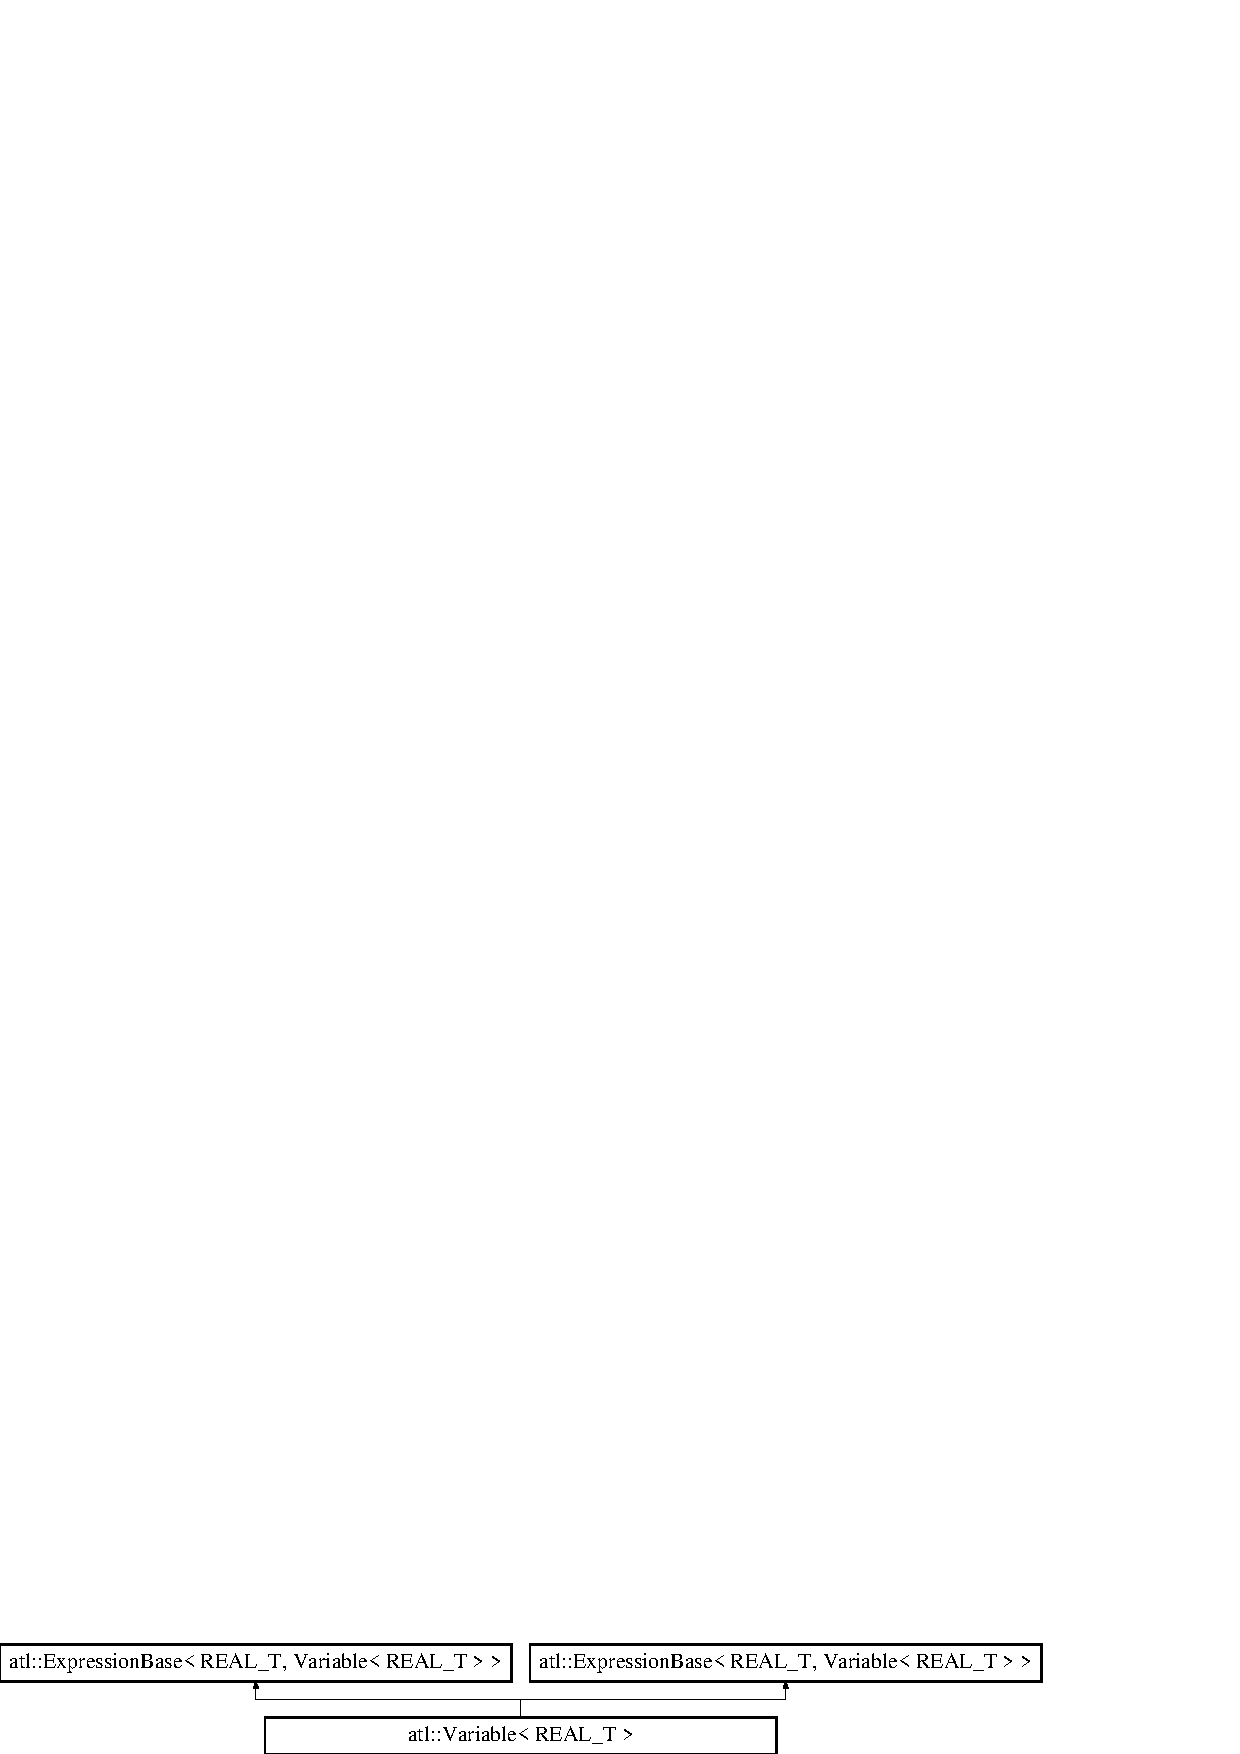
\includegraphics[height=1.717791cm]{structatl_1_1_variable}
\end{center}
\end{figure}
\subsection*{Public Types}
\begin{DoxyCompactItemize}
\item 
\hypertarget{structatl_1_1_variable_a1e4e292405873d1ddf28a7a629a11be4}{typedef R\+E\+A\+L\+\_\+\+T {\bfseries base\+\_\+type}}\label{structatl_1_1_variable_a1e4e292405873d1ddf28a7a629a11be4}

\item 
\hypertarget{structatl_1_1_variable_a1e4e292405873d1ddf28a7a629a11be4}{typedef R\+E\+A\+L\+\_\+\+T {\bfseries base\+\_\+type}}\label{structatl_1_1_variable_a1e4e292405873d1ddf28a7a629a11be4}

\end{DoxyCompactItemize}
\subsection*{Public Member Functions}
\begin{DoxyCompactItemize}
\item 
\hypertarget{structatl_1_1_variable_a0089f2d112ea67897ac2e23033686279}{{\bfseries Variable} (R\+E\+A\+L\+\_\+\+T v=static\+\_\+cast$<$ R\+E\+A\+L\+\_\+\+T $>$(0.\+0))}\label{structatl_1_1_variable_a0089f2d112ea67897ac2e23033686279}

\item 
\hypertarget{structatl_1_1_variable_a64f472f5f036b681d9e9b35f3de96a1e}{{\bfseries Variable} (const \hyperlink{structatl_1_1_variable}{Variable}$<$ R\+E\+A\+L\+\_\+\+T $>$ \&other)}\label{structatl_1_1_variable_a64f472f5f036b681d9e9b35f3de96a1e}

\item 
\hypertarget{structatl_1_1_variable_a6237645a2e54443ec0c101d089c5f834}{\hyperlink{structatl_1_1_variable}{Variable} \& {\bfseries operator=} (const R\+E\+A\+L\+\_\+\+T \&v)}\label{structatl_1_1_variable_a6237645a2e54443ec0c101d089c5f834}

\item 
\hypertarget{structatl_1_1_variable_a900d049c0f459456bd19f2bdbbb76ab3}{{\footnotesize template$<$class A $>$ }\\{\bfseries Variable} (const \hyperlink{structatl_1_1_expression_base}{Expression\+Base}$<$ R\+E\+A\+L\+\_\+\+T, A $>$ \&exp)}\label{structatl_1_1_variable_a900d049c0f459456bd19f2bdbbb76ab3}

\item 
\hypertarget{structatl_1_1_variable_abfa1e5ed61daa1b25668f3afd1bfd125}{{\footnotesize template$<$class A $>$ }\\\hyperlink{structatl_1_1_variable}{Variable} \& {\bfseries operator=} (const \hyperlink{structatl_1_1_expression_base}{Expression\+Base}$<$ R\+E\+A\+L\+\_\+\+T, A $>$ \&exp)}\label{structatl_1_1_variable_abfa1e5ed61daa1b25668f3afd1bfd125}

\item 
\hypertarget{structatl_1_1_variable_aad8e1d6b2c5258b17020f8ee694ffb95}{\hyperlink{structatl_1_1_variable}{Variable} \& {\bfseries operator+=} (const R\+E\+A\+L\+\_\+\+T \&val)}\label{structatl_1_1_variable_aad8e1d6b2c5258b17020f8ee694ffb95}

\item 
\hypertarget{structatl_1_1_variable_a575ec695135b3abdcae2141434e87100}{{\footnotesize template$<$class A $>$ }\\\hyperlink{structatl_1_1_variable}{Variable} \& {\bfseries operator+=} (const \hyperlink{structatl_1_1_expression_base}{Expression\+Base}$<$ R\+E\+A\+L\+\_\+\+T, A $>$ \&exp)}\label{structatl_1_1_variable_a575ec695135b3abdcae2141434e87100}

\item 
\hypertarget{structatl_1_1_variable_ab822ce13f7a8d979c7ae0253a5adea07}{\hyperlink{structatl_1_1_variable}{Variable} \& {\bfseries operator-\/=} (const R\+E\+A\+L\+\_\+\+T \&val)}\label{structatl_1_1_variable_ab822ce13f7a8d979c7ae0253a5adea07}

\item 
\hypertarget{structatl_1_1_variable_ad1be31d4f6e25cb4e26b0fb6cf61e91a}{{\footnotesize template$<$class A $>$ }\\\hyperlink{structatl_1_1_variable}{Variable} \& {\bfseries operator-\/=} (const \hyperlink{structatl_1_1_expression_base}{Expression\+Base}$<$ R\+E\+A\+L\+\_\+\+T, A $>$ \&exp)}\label{structatl_1_1_variable_ad1be31d4f6e25cb4e26b0fb6cf61e91a}

\item 
\hypertarget{structatl_1_1_variable_a625c5a60771393a83e51bd605132987a}{\hyperlink{structatl_1_1_variable}{Variable} \& {\bfseries operator$\ast$=} (const R\+E\+A\+L\+\_\+\+T \&val)}\label{structatl_1_1_variable_a625c5a60771393a83e51bd605132987a}

\item 
\hypertarget{structatl_1_1_variable_abd8effad2f281d679c6cc4ad8d92bcb5}{{\footnotesize template$<$class A $>$ }\\\hyperlink{structatl_1_1_variable}{Variable} \& {\bfseries operator$\ast$=} (const \hyperlink{structatl_1_1_expression_base}{Expression\+Base}$<$ R\+E\+A\+L\+\_\+\+T, A $>$ \&exp)}\label{structatl_1_1_variable_abd8effad2f281d679c6cc4ad8d92bcb5}

\item 
\hypertarget{structatl_1_1_variable_afd5cf7762056c7157936b928f9d98007}{\hyperlink{structatl_1_1_variable}{Variable} \& {\bfseries operator/=} (const R\+E\+A\+L\+\_\+\+T \&val)}\label{structatl_1_1_variable_afd5cf7762056c7157936b928f9d98007}

\item 
\hypertarget{structatl_1_1_variable_a0d179dc181b83542633581994396b719}{{\footnotesize template$<$class A $>$ }\\\hyperlink{structatl_1_1_variable}{Variable} \& {\bfseries operator/=} (const \hyperlink{structatl_1_1_expression_base}{Expression\+Base}$<$ R\+E\+A\+L\+\_\+\+T, A $>$ \&exp)}\label{structatl_1_1_variable_a0d179dc181b83542633581994396b719}

\item 
\hypertarget{structatl_1_1_variable_ac0b77adb93d2f9cb6ba8f58ff7082c66}{\hyperlink{structatl_1_1_variable}{Variable} \& {\bfseries operator++} ()}\label{structatl_1_1_variable_ac0b77adb93d2f9cb6ba8f58ff7082c66}

\item 
\hypertarget{structatl_1_1_variable_aa48b49bfaa75a7eb17c26fe632c4bbbb}{const \hyperlink{structatl_1_1_variable}{Variable} {\bfseries operator++} (int i)}\label{structatl_1_1_variable_aa48b49bfaa75a7eb17c26fe632c4bbbb}

\item 
\hypertarget{structatl_1_1_variable_a9f5bfc096684109e36d3d397fad4b337}{\hyperlink{structatl_1_1_variable}{Variable} \& {\bfseries operator-\/-\/} ()}\label{structatl_1_1_variable_a9f5bfc096684109e36d3d397fad4b337}

\item 
\hypertarget{structatl_1_1_variable_ad54d90109a8d0242f291579581ed746b}{const \hyperlink{structatl_1_1_variable}{Variable} {\bfseries operator-\/-\/} (int i)}\label{structatl_1_1_variable_ad54d90109a8d0242f291579581ed746b}

\item 
\hypertarget{structatl_1_1_variable_a75e72fa736f11f18a328fd18172c6071}{const R\+E\+A\+L\+\_\+\+T {\bfseries Get\+Value} () const }\label{structatl_1_1_variable_a75e72fa736f11f18a328fd18172c6071}

\item 
\hypertarget{structatl_1_1_variable_a4e4c6c390e81522d7862fe5b9b803a1e}{const R\+E\+A\+L\+\_\+\+T {\bfseries Get\+Value} (size\+\_\+t i, size\+\_\+t j=0) const }\label{structatl_1_1_variable_a4e4c6c390e81522d7862fe5b9b803a1e}

\item 
\hypertarget{structatl_1_1_variable_a0060cd8c8081cb4e5c2a3a9967e10737}{void {\bfseries Push\+Ids} (typename \hyperlink{structatl_1_1_stack_entry}{atl\+::\+Stack\+Entry}$<$ R\+E\+A\+L\+\_\+\+T $>$\+::vi\+\_\+storage \&ids) const }\label{structatl_1_1_variable_a0060cd8c8081cb4e5c2a3a9967e10737}

\item 
\hypertarget{structatl_1_1_variable_aa2ab761e1449b8efcb3b86991a9dc764}{void {\bfseries Push\+Ids} (typename \hyperlink{structatl_1_1_stack_entry}{atl\+::\+Stack\+Entry}$<$ R\+E\+A\+L\+\_\+\+T $>$\+::vi\+\_\+storage \&ids, size\+\_\+t i, size\+\_\+t j=0) const }\label{structatl_1_1_variable_aa2ab761e1449b8efcb3b86991a9dc764}

\item 
\hypertarget{structatl_1_1_variable_a16eecc46193577d28dbe49b900f39701}{R\+E\+A\+L\+\_\+\+T {\bfseries Evaluate\+Derivative} (uint32\+\_\+t a) const }\label{structatl_1_1_variable_a16eecc46193577d28dbe49b900f39701}

\item 
\hypertarget{structatl_1_1_variable_ae0e92ce16a480a08f19cbba21d784540}{R\+E\+A\+L\+\_\+\+T {\bfseries Evaluate\+Derivative} (uint32\+\_\+t a, uint32\+\_\+t b) const }\label{structatl_1_1_variable_ae0e92ce16a480a08f19cbba21d784540}

\item 
\hypertarget{structatl_1_1_variable_a2d32c28f89eebef1d11430548e15fb60}{R\+E\+A\+L\+\_\+\+T {\bfseries Evaluate\+Derivative} (uint32\+\_\+t x, uint32\+\_\+t y, uint32\+\_\+t z) const }\label{structatl_1_1_variable_a2d32c28f89eebef1d11430548e15fb60}

\item 
\hypertarget{structatl_1_1_variable_a231e419a98a1ae0eef903cd25c8cc025}{R\+E\+A\+L\+\_\+\+T {\bfseries Evaluate\+Derivative} (uint32\+\_\+t a, size\+\_\+t i, size\+\_\+t j=0) const }\label{structatl_1_1_variable_a231e419a98a1ae0eef903cd25c8cc025}

\item 
\hypertarget{structatl_1_1_variable_a05cda7ab0ee9d700edb57cb5c1768005}{R\+E\+A\+L\+\_\+\+T {\bfseries Evaluate\+Derivative} (uint32\+\_\+t a, uint32\+\_\+t b, size\+\_\+t i, size\+\_\+t j=0) const }\label{structatl_1_1_variable_a05cda7ab0ee9d700edb57cb5c1768005}

\item 
\hypertarget{structatl_1_1_variable_a31574d4c65eca8ad0e1553525f568ca5}{R\+E\+A\+L\+\_\+\+T {\bfseries Evaluate\+Derivative} (uint32\+\_\+t x, uint32\+\_\+t y, uint32\+\_\+t z, size\+\_\+t i, size\+\_\+t j=0) const }\label{structatl_1_1_variable_a31574d4c65eca8ad0e1553525f568ca5}

\item 
\hypertarget{structatl_1_1_variable_a8014f00f3b2233bf46a83395e1bb9d79}{size\+\_\+t {\bfseries Get\+Columns} () const }\label{structatl_1_1_variable_a8014f00f3b2233bf46a83395e1bb9d79}

\item 
\hypertarget{structatl_1_1_variable_a92ae914f1792b5cdc2abc3c8a5f1e4d2}{size\+\_\+t {\bfseries Get\+Rows} () const }\label{structatl_1_1_variable_a92ae914f1792b5cdc2abc3c8a5f1e4d2}

\item 
\hypertarget{structatl_1_1_variable_a0e6e6a7b6dd2cc83d170beccbe900d36}{bool {\bfseries Is\+Scalar} () const }\label{structatl_1_1_variable_a0e6e6a7b6dd2cc83d170beccbe900d36}

\item 
\hypertarget{structatl_1_1_variable_a0089f2d112ea67897ac2e23033686279}{{\bfseries Variable} (R\+E\+A\+L\+\_\+\+T v=static\+\_\+cast$<$ R\+E\+A\+L\+\_\+\+T $>$(0.\+0))}\label{structatl_1_1_variable_a0089f2d112ea67897ac2e23033686279}

\item 
\hypertarget{structatl_1_1_variable_a64f472f5f036b681d9e9b35f3de96a1e}{{\bfseries Variable} (const \hyperlink{structatl_1_1_variable}{Variable}$<$ R\+E\+A\+L\+\_\+\+T $>$ \&other)}\label{structatl_1_1_variable_a64f472f5f036b681d9e9b35f3de96a1e}

\item 
\hypertarget{structatl_1_1_variable_a6237645a2e54443ec0c101d089c5f834}{\hyperlink{structatl_1_1_variable}{Variable} \& {\bfseries operator=} (const R\+E\+A\+L\+\_\+\+T \&v)}\label{structatl_1_1_variable_a6237645a2e54443ec0c101d089c5f834}

\item 
\hypertarget{structatl_1_1_variable_a900d049c0f459456bd19f2bdbbb76ab3}{{\footnotesize template$<$class A $>$ }\\{\bfseries Variable} (const \hyperlink{structatl_1_1_expression_base}{Expression\+Base}$<$ R\+E\+A\+L\+\_\+\+T, A $>$ \&exp)}\label{structatl_1_1_variable_a900d049c0f459456bd19f2bdbbb76ab3}

\item 
R\+E\+A\+L\+\_\+\+T \& \hyperlink{structatl_1_1_variable_a6a78210005f19418b6a97745dacdb37b}{operator$\ast$} ()
\item 
const R\+E\+A\+L\+\_\+\+T \& \hyperlink{structatl_1_1_variable_a8ab38ec15b81342e5c5f5611dcc5888a}{operator$\ast$} () const 
\item 
\hypertarget{structatl_1_1_variable_abfa1e5ed61daa1b25668f3afd1bfd125}{{\footnotesize template$<$class A $>$ }\\\hyperlink{structatl_1_1_variable}{Variable} \& {\bfseries operator=} (const \hyperlink{structatl_1_1_expression_base}{Expression\+Base}$<$ R\+E\+A\+L\+\_\+\+T, A $>$ \&exp)}\label{structatl_1_1_variable_abfa1e5ed61daa1b25668f3afd1bfd125}

\item 
\hypertarget{structatl_1_1_variable_aad92665db0c50f28a772d22d23cb5e83}{{\footnotesize template$<$class A $>$ }\\\hyperlink{structatl_1_1_variable}{Variable} \& {\bfseries Assign} (const \hyperlink{structatl_1_1_expression_base}{Expression\+Base}$<$ R\+E\+A\+L\+\_\+\+T, A $>$ \&exp)}\label{structatl_1_1_variable_aad92665db0c50f28a772d22d23cb5e83}

\item 
{\footnotesize template$<$class A $>$ }\\\hyperlink{structatl_1_1_variable}{Variable} \& \hyperlink{structatl_1_1_variable_a753439be059d8e894aa72c4a521a193d}{Assign} (\hyperlink{classatl_1_1_tape}{atl\+::\+Tape}$<$ R\+E\+A\+L\+\_\+\+T $>$ \&tape, const \hyperlink{structatl_1_1_expression_base}{Expression\+Base}$<$ R\+E\+A\+L\+\_\+\+T, A $>$ \&exp)
\item 
{\footnotesize template$<$class A $>$ }\\\hyperlink{structatl_1_1_variable}{Variable} \& \hyperlink{structatl_1_1_variable_a2a5fbe56961922c12103b72855d438fe}{Assign} (const \hyperlink{structatl_1_1_expression_base}{Expression\+Base}$<$ R\+E\+A\+L\+\_\+\+T, A $>$ \&exp, size\+\_\+t index)
\item 
{\footnotesize template$<$class A $>$ }\\\hyperlink{structatl_1_1_variable}{Variable} \& \hyperlink{structatl_1_1_variable_ac15e910a224d189944c71776ceb67cc1}{Assign} (\hyperlink{classatl_1_1_tape}{atl\+::\+Tape}$<$ R\+E\+A\+L\+\_\+\+T $>$ \&tape, const \hyperlink{structatl_1_1_expression_base}{Expression\+Base}$<$ R\+E\+A\+L\+\_\+\+T, A $>$ \&exp, size\+\_\+t index)
\item 
\hypertarget{structatl_1_1_variable_aad8e1d6b2c5258b17020f8ee694ffb95}{\hyperlink{structatl_1_1_variable}{Variable} \& {\bfseries operator+=} (const R\+E\+A\+L\+\_\+\+T \&val)}\label{structatl_1_1_variable_aad8e1d6b2c5258b17020f8ee694ffb95}

\item 
\hypertarget{structatl_1_1_variable_a575ec695135b3abdcae2141434e87100}{{\footnotesize template$<$class A $>$ }\\\hyperlink{structatl_1_1_variable}{Variable} \& {\bfseries operator+=} (const \hyperlink{structatl_1_1_expression_base}{Expression\+Base}$<$ R\+E\+A\+L\+\_\+\+T, A $>$ \&exp)}\label{structatl_1_1_variable_a575ec695135b3abdcae2141434e87100}

\item 
\hypertarget{structatl_1_1_variable_ab822ce13f7a8d979c7ae0253a5adea07}{\hyperlink{structatl_1_1_variable}{Variable} \& {\bfseries operator-\/=} (const R\+E\+A\+L\+\_\+\+T \&val)}\label{structatl_1_1_variable_ab822ce13f7a8d979c7ae0253a5adea07}

\item 
\hypertarget{structatl_1_1_variable_ad1be31d4f6e25cb4e26b0fb6cf61e91a}{{\footnotesize template$<$class A $>$ }\\\hyperlink{structatl_1_1_variable}{Variable} \& {\bfseries operator-\/=} (const \hyperlink{structatl_1_1_expression_base}{Expression\+Base}$<$ R\+E\+A\+L\+\_\+\+T, A $>$ \&exp)}\label{structatl_1_1_variable_ad1be31d4f6e25cb4e26b0fb6cf61e91a}

\item 
\hypertarget{structatl_1_1_variable_a625c5a60771393a83e51bd605132987a}{\hyperlink{structatl_1_1_variable}{Variable} \& {\bfseries operator$\ast$=} (const R\+E\+A\+L\+\_\+\+T \&val)}\label{structatl_1_1_variable_a625c5a60771393a83e51bd605132987a}

\item 
\hypertarget{structatl_1_1_variable_abd8effad2f281d679c6cc4ad8d92bcb5}{{\footnotesize template$<$class A $>$ }\\\hyperlink{structatl_1_1_variable}{Variable} \& {\bfseries operator$\ast$=} (const \hyperlink{structatl_1_1_expression_base}{Expression\+Base}$<$ R\+E\+A\+L\+\_\+\+T, A $>$ \&exp)}\label{structatl_1_1_variable_abd8effad2f281d679c6cc4ad8d92bcb5}

\item 
\hypertarget{structatl_1_1_variable_afd5cf7762056c7157936b928f9d98007}{\hyperlink{structatl_1_1_variable}{Variable} \& {\bfseries operator/=} (const R\+E\+A\+L\+\_\+\+T \&val)}\label{structatl_1_1_variable_afd5cf7762056c7157936b928f9d98007}

\item 
\hypertarget{structatl_1_1_variable_a0d179dc181b83542633581994396b719}{{\footnotesize template$<$class A $>$ }\\\hyperlink{structatl_1_1_variable}{Variable} \& {\bfseries operator/=} (const \hyperlink{structatl_1_1_expression_base}{Expression\+Base}$<$ R\+E\+A\+L\+\_\+\+T, A $>$ \&exp)}\label{structatl_1_1_variable_a0d179dc181b83542633581994396b719}

\item 
\hypertarget{structatl_1_1_variable_ac0b77adb93d2f9cb6ba8f58ff7082c66}{\hyperlink{structatl_1_1_variable}{Variable} \& {\bfseries operator++} ()}\label{structatl_1_1_variable_ac0b77adb93d2f9cb6ba8f58ff7082c66}

\item 
\hypertarget{structatl_1_1_variable_aa48b49bfaa75a7eb17c26fe632c4bbbb}{const \hyperlink{structatl_1_1_variable}{Variable} {\bfseries operator++} (int i)}\label{structatl_1_1_variable_aa48b49bfaa75a7eb17c26fe632c4bbbb}

\item 
\hypertarget{structatl_1_1_variable_a9f5bfc096684109e36d3d397fad4b337}{\hyperlink{structatl_1_1_variable}{Variable} \& {\bfseries operator-\/-\/} ()}\label{structatl_1_1_variable_a9f5bfc096684109e36d3d397fad4b337}

\item 
\hypertarget{structatl_1_1_variable_ad54d90109a8d0242f291579581ed746b}{const \hyperlink{structatl_1_1_variable}{Variable} {\bfseries operator-\/-\/} (int i)}\label{structatl_1_1_variable_ad54d90109a8d0242f291579581ed746b}

\item 
\hypertarget{structatl_1_1_variable_a75e72fa736f11f18a328fd18172c6071}{const R\+E\+A\+L\+\_\+\+T {\bfseries Get\+Value} () const }\label{structatl_1_1_variable_a75e72fa736f11f18a328fd18172c6071}

\item 
\hypertarget{structatl_1_1_variable_a4e4c6c390e81522d7862fe5b9b803a1e}{const R\+E\+A\+L\+\_\+\+T {\bfseries Get\+Value} (size\+\_\+t i, size\+\_\+t j=0) const }\label{structatl_1_1_variable_a4e4c6c390e81522d7862fe5b9b803a1e}

\item 
bool \hyperlink{structatl_1_1_variable_af043141beb92eff684c7cd28618f362c}{Is\+Nonlinear} () const 
\item 
\hypertarget{structatl_1_1_variable_a0060cd8c8081cb4e5c2a3a9967e10737}{void {\bfseries Push\+Ids} (typename \hyperlink{structatl_1_1_stack_entry}{atl\+::\+Stack\+Entry}$<$ R\+E\+A\+L\+\_\+\+T $>$\+::vi\+\_\+storage \&ids) const }\label{structatl_1_1_variable_a0060cd8c8081cb4e5c2a3a9967e10737}

\item 
\hypertarget{structatl_1_1_variable_aa2ab761e1449b8efcb3b86991a9dc764}{void {\bfseries Push\+Ids} (typename \hyperlink{structatl_1_1_stack_entry}{atl\+::\+Stack\+Entry}$<$ R\+E\+A\+L\+\_\+\+T $>$\+::vi\+\_\+storage \&ids, size\+\_\+t i, size\+\_\+t j=0) const }\label{structatl_1_1_variable_aa2ab761e1449b8efcb3b86991a9dc764}

\item 
\hypertarget{structatl_1_1_variable_a366f95a9d1f2b2140f1f90032301d263}{R\+E\+A\+L\+\_\+\+T {\bfseries Evaluate\+Derivative} (uint32\+\_\+t x) const }\label{structatl_1_1_variable_a366f95a9d1f2b2140f1f90032301d263}

\item 
\hypertarget{structatl_1_1_variable_a3bc7db32a25fe488e1390d81725d6d67}{R\+E\+A\+L\+\_\+\+T {\bfseries Evaluate\+Derivative} (uint32\+\_\+t x, uint32\+\_\+t y) const }\label{structatl_1_1_variable_a3bc7db32a25fe488e1390d81725d6d67}

\item 
\hypertarget{structatl_1_1_variable_a2d32c28f89eebef1d11430548e15fb60}{R\+E\+A\+L\+\_\+\+T {\bfseries Evaluate\+Derivative} (uint32\+\_\+t x, uint32\+\_\+t y, uint32\+\_\+t z) const }\label{structatl_1_1_variable_a2d32c28f89eebef1d11430548e15fb60}

\item 
\hypertarget{structatl_1_1_variable_ad222f1a0b1655d9a82ba2ce51fa2009f}{R\+E\+A\+L\+\_\+\+T {\bfseries Evaluate\+Derivative} (uint32\+\_\+t x, size\+\_\+t i, size\+\_\+t j=0) const }\label{structatl_1_1_variable_ad222f1a0b1655d9a82ba2ce51fa2009f}

\item 
\hypertarget{structatl_1_1_variable_ad8cb122781aab4ae18fe0898cc367567}{R\+E\+A\+L\+\_\+\+T {\bfseries Evaluate\+Derivative} (uint32\+\_\+t x, uint32\+\_\+t y, size\+\_\+t i, size\+\_\+t j=0) const }\label{structatl_1_1_variable_ad8cb122781aab4ae18fe0898cc367567}

\item 
\hypertarget{structatl_1_1_variable_a31574d4c65eca8ad0e1553525f568ca5}{R\+E\+A\+L\+\_\+\+T {\bfseries Evaluate\+Derivative} (uint32\+\_\+t x, uint32\+\_\+t y, uint32\+\_\+t z, size\+\_\+t i, size\+\_\+t j=0) const }\label{structatl_1_1_variable_a31574d4c65eca8ad0e1553525f568ca5}

\item 
\hypertarget{structatl_1_1_variable_a8014f00f3b2233bf46a83395e1bb9d79}{size\+\_\+t {\bfseries Get\+Columns} () const }\label{structatl_1_1_variable_a8014f00f3b2233bf46a83395e1bb9d79}

\item 
\hypertarget{structatl_1_1_variable_a92ae914f1792b5cdc2abc3c8a5f1e4d2}{size\+\_\+t {\bfseries Get\+Rows} () const }\label{structatl_1_1_variable_a92ae914f1792b5cdc2abc3c8a5f1e4d2}

\item 
\hypertarget{structatl_1_1_variable_a0e6e6a7b6dd2cc83d170beccbe900d36}{bool {\bfseries Is\+Scalar} () const }\label{structatl_1_1_variable_a0e6e6a7b6dd2cc83d170beccbe900d36}

\item 
\hypertarget{structatl_1_1_variable_a1d77872acc73fb4eaa3d55419cd4635c}{const std\+::string {\bfseries To\+Expression\+Template\+String} () const }\label{structatl_1_1_variable_a1d77872acc73fb4eaa3d55419cd4635c}

\end{DoxyCompactItemize}
\subsection*{Public Attributes}
\begin{DoxyCompactItemize}
\item 
\hypertarget{structatl_1_1_variable_a009aa3303bc1cca1d4df22a8404eec28}{\hyperlink{structatl_1_1_variable_info}{atl\+::\+Variable\+Info}$<$ R\+E\+A\+L\+\_\+\+T $>$ $\ast$ {\bfseries info} = new \hyperlink{structatl_1_1_variable_info}{atl\+::\+Variable\+Info}$<$R\+E\+A\+L\+\_\+\+T$>$()}\label{structatl_1_1_variable_a009aa3303bc1cca1d4df22a8404eec28}

\end{DoxyCompactItemize}
\subsection*{Static Public Attributes}
\begin{DoxyCompactItemize}
\item 
\hypertarget{structatl_1_1_variable_a8aa8cc1649ff93f180fc1185857d9f53}{static \hyperlink{classatl_1_1_tape}{Tape}$<$ R\+E\+A\+L\+\_\+\+T $>$ {\bfseries tape}}\label{structatl_1_1_variable_a8aa8cc1649ff93f180fc1185857d9f53}

\end{DoxyCompactItemize}


\subsection{Member Function Documentation}
\hypertarget{structatl_1_1_variable_a753439be059d8e894aa72c4a521a193d}{\index{atl\+::\+Variable@{atl\+::\+Variable}!Assign@{Assign}}
\index{Assign@{Assign}!atl\+::\+Variable@{atl\+::\+Variable}}
\subsubsection[{Assign}]{\setlength{\rightskip}{0pt plus 5cm}template$<$typename R\+E\+A\+L\+\_\+\+T$>$ template$<$class A $>$ {\bf Variable}\& {\bf atl\+::\+Variable}$<$ R\+E\+A\+L\+\_\+\+T $>$\+::Assign (
\begin{DoxyParamCaption}
\item[{{\bf atl\+::\+Tape}$<$ R\+E\+A\+L\+\_\+\+T $>$ \&}]{tape, }
\item[{const {\bf Expression\+Base}$<$ R\+E\+A\+L\+\_\+\+T, A $>$ \&}]{exp}
\end{DoxyParamCaption}
)\hspace{0.3cm}{\ttfamily [inline]}}}\label{structatl_1_1_variable_a753439be059d8e894aa72c4a521a193d}
Assign using the specified tape structure.


\begin{DoxyParams}{Parameters}
{\em tape} & \\
\hline
{\em exp} & \\
\hline
\end{DoxyParams}
\begin{DoxyReturn}{Returns}

\end{DoxyReturn}
\hypertarget{structatl_1_1_variable_a2a5fbe56961922c12103b72855d438fe}{\index{atl\+::\+Variable@{atl\+::\+Variable}!Assign@{Assign}}
\index{Assign@{Assign}!atl\+::\+Variable@{atl\+::\+Variable}}
\subsubsection[{Assign}]{\setlength{\rightskip}{0pt plus 5cm}template$<$typename R\+E\+A\+L\+\_\+\+T$>$ template$<$class A $>$ {\bf Variable}\& {\bf atl\+::\+Variable}$<$ R\+E\+A\+L\+\_\+\+T $>$\+::Assign (
\begin{DoxyParamCaption}
\item[{const {\bf Expression\+Base}$<$ R\+E\+A\+L\+\_\+\+T, A $>$ \&}]{exp, }
\item[{size\+\_\+t}]{index}
\end{DoxyParamCaption}
)\hspace{0.3cm}{\ttfamily [inline]}}}\label{structatl_1_1_variable_a2a5fbe56961922c12103b72855d438fe}
Assign using a tape entry at at the specified index.


\begin{DoxyParams}{Parameters}
{\em exp} & \\
\hline
{\em index} & \\
\hline
\end{DoxyParams}
\begin{DoxyReturn}{Returns}

\end{DoxyReturn}
\hypertarget{structatl_1_1_variable_ac15e910a224d189944c71776ceb67cc1}{\index{atl\+::\+Variable@{atl\+::\+Variable}!Assign@{Assign}}
\index{Assign@{Assign}!atl\+::\+Variable@{atl\+::\+Variable}}
\subsubsection[{Assign}]{\setlength{\rightskip}{0pt plus 5cm}template$<$typename R\+E\+A\+L\+\_\+\+T$>$ template$<$class A $>$ {\bf Variable}\& {\bf atl\+::\+Variable}$<$ R\+E\+A\+L\+\_\+\+T $>$\+::Assign (
\begin{DoxyParamCaption}
\item[{{\bf atl\+::\+Tape}$<$ R\+E\+A\+L\+\_\+\+T $>$ \&}]{tape, }
\item[{const {\bf Expression\+Base}$<$ R\+E\+A\+L\+\_\+\+T, A $>$ \&}]{exp, }
\item[{size\+\_\+t}]{index}
\end{DoxyParamCaption}
)\hspace{0.3cm}{\ttfamily [inline]}}}\label{structatl_1_1_variable_ac15e910a224d189944c71776ceb67cc1}
Assign using a specified tape at a specified entry at index.


\begin{DoxyParams}{Parameters}
{\em exp} & \\
\hline
{\em index} & \\
\hline
\end{DoxyParams}
\begin{DoxyReturn}{Returns}

\end{DoxyReturn}
\hypertarget{structatl_1_1_variable_af043141beb92eff684c7cd28618f362c}{\index{atl\+::\+Variable@{atl\+::\+Variable}!Is\+Nonlinear@{Is\+Nonlinear}}
\index{Is\+Nonlinear@{Is\+Nonlinear}!atl\+::\+Variable@{atl\+::\+Variable}}
\subsubsection[{Is\+Nonlinear}]{\setlength{\rightskip}{0pt plus 5cm}template$<$typename R\+E\+A\+L\+\_\+\+T$>$ bool {\bf atl\+::\+Variable}$<$ R\+E\+A\+L\+\_\+\+T $>$\+::Is\+Nonlinear (
\begin{DoxyParamCaption}
{}
\end{DoxyParamCaption}
) const\hspace{0.3cm}{\ttfamily [inline]}}}\label{structatl_1_1_variable_af043141beb92eff684c7cd28618f362c}
Returns false.

\begin{DoxyReturn}{Returns}

\end{DoxyReturn}
\hypertarget{structatl_1_1_variable_a6a78210005f19418b6a97745dacdb37b}{\index{atl\+::\+Variable@{atl\+::\+Variable}!operator$\ast$@{operator$\ast$}}
\index{operator$\ast$@{operator$\ast$}!atl\+::\+Variable@{atl\+::\+Variable}}
\subsubsection[{operator$\ast$}]{\setlength{\rightskip}{0pt plus 5cm}template$<$typename R\+E\+A\+L\+\_\+\+T$>$ R\+E\+A\+L\+\_\+\+T\& {\bf atl\+::\+Variable}$<$ R\+E\+A\+L\+\_\+\+T $>$\+::operator$\ast$ (
\begin{DoxyParamCaption}
{}
\end{DoxyParamCaption}
)\hspace{0.3cm}{\ttfamily [inline]}}}\label{structatl_1_1_variable_a6a78210005f19418b6a97745dacdb37b}
Returns a reference to the raw value.

\begin{DoxyReturn}{Returns}

\end{DoxyReturn}
\hypertarget{structatl_1_1_variable_a8ab38ec15b81342e5c5f5611dcc5888a}{\index{atl\+::\+Variable@{atl\+::\+Variable}!operator$\ast$@{operator$\ast$}}
\index{operator$\ast$@{operator$\ast$}!atl\+::\+Variable@{atl\+::\+Variable}}
\subsubsection[{operator$\ast$}]{\setlength{\rightskip}{0pt plus 5cm}template$<$typename R\+E\+A\+L\+\_\+\+T$>$ const R\+E\+A\+L\+\_\+\+T\& {\bf atl\+::\+Variable}$<$ R\+E\+A\+L\+\_\+\+T $>$\+::operator$\ast$ (
\begin{DoxyParamCaption}
{}
\end{DoxyParamCaption}
) const\hspace{0.3cm}{\ttfamily [inline]}}}\label{structatl_1_1_variable_a8ab38ec15b81342e5c5f5611dcc5888a}
Returns a const reference to the raw value.

\begin{DoxyReturn}{Returns}

\end{DoxyReturn}


The documentation for this struct was generated from the following file\+:\begin{DoxyCompactItemize}
\item 
A\+T\+L2/Variable.\+hpp\end{DoxyCompactItemize}

\hypertarget{classatl_1_1_variable_id_generator}{\section{atl\+:\+:Variable\+Id\+Generator Class Reference}
\label{classatl_1_1_variable_id_generator}\index{atl\+::\+Variable\+Id\+Generator@{atl\+::\+Variable\+Id\+Generator}}
}


{\ttfamily \#include $<$Variable\+Info.\+hpp$>$}

\subsection*{Public Member Functions}
\begin{DoxyCompactItemize}
\item 
\hypertarget{classatl_1_1_variable_id_generator_a01360832f33700e4fd86b6e237996ffd}{const uint32\+\_\+t {\bfseries next} ()}\label{classatl_1_1_variable_id_generator_a01360832f33700e4fd86b6e237996ffd}

\item 
\hypertarget{classatl_1_1_variable_id_generator_a98643dc9bff062bf39dc5de514b89e18}{void {\bfseries release} (const uint32\+\_\+t \&id)}\label{classatl_1_1_variable_id_generator_a98643dc9bff062bf39dc5de514b89e18}

\item 
\hypertarget{classatl_1_1_variable_id_generator_aa449ce6f8d2433a50fd38b8baa28e72a}{const uint32\+\_\+t {\bfseries current} ()}\label{classatl_1_1_variable_id_generator_aa449ce6f8d2433a50fd38b8baa28e72a}

\item 
\hypertarget{classatl_1_1_variable_id_generator_a01360832f33700e4fd86b6e237996ffd}{const uint32\+\_\+t {\bfseries next} ()}\label{classatl_1_1_variable_id_generator_a01360832f33700e4fd86b6e237996ffd}

\item 
\hypertarget{classatl_1_1_variable_id_generator_a98643dc9bff062bf39dc5de514b89e18}{void {\bfseries release} (const uint32\+\_\+t \&id)}\label{classatl_1_1_variable_id_generator_a98643dc9bff062bf39dc5de514b89e18}

\item 
\hypertarget{classatl_1_1_variable_id_generator_aa449ce6f8d2433a50fd38b8baa28e72a}{const uint32\+\_\+t {\bfseries current} ()}\label{classatl_1_1_variable_id_generator_aa449ce6f8d2433a50fd38b8baa28e72a}

\end{DoxyCompactItemize}
\subsection*{Static Public Member Functions}
\begin{DoxyCompactItemize}
\item 
\hypertarget{classatl_1_1_variable_id_generator_a780b39026099c6556015bfc73f0cfc27}{static std\+::shared\+\_\+ptr\\*
$<$ \hyperlink{classatl_1_1_variable_id_generator}{Variable\+Id\+Generator} $>$ {\bfseries instance} ()}\label{classatl_1_1_variable_id_generator_a780b39026099c6556015bfc73f0cfc27}

\item 
\hypertarget{classatl_1_1_variable_id_generator_a1cf81533df4cdd7c6cc7a1d2f100388a}{static std\+::shared\+\_\+ptr\\*
$<$ \hyperlink{classatl_1_1_variable_id_generator}{Variable\+Id\+Generator} $>$ {\bfseries instance} ()}\label{classatl_1_1_variable_id_generator_a1cf81533df4cdd7c6cc7a1d2f100388a}

\end{DoxyCompactItemize}
\subsection*{Public Attributes}
\begin{DoxyCompactItemize}
\item 
\hypertarget{classatl_1_1_variable_id_generator_a5c8dd40ad503d55f82520ced39a9a5f0}{std\+::atomic$<$ uint32\+\_\+t $>$ {\bfseries \+\_\+id}}\label{classatl_1_1_variable_id_generator_a5c8dd40ad503d55f82520ced39a9a5f0}

\end{DoxyCompactItemize}


\subsection{Detailed Description}
Creates a unique identifier for variables. Identifiers are recyclable. \begin{DoxyReturn}{Returns}

\end{DoxyReturn}


The documentation for this class was generated from the following file\+:\begin{DoxyCompactItemize}
\item 
A\+T\+L2/Variable\+Info.\+hpp\end{DoxyCompactItemize}

\hypertarget{structatl_1_1_variable_info}{\section{atl\+:\+:Variable\+Info$<$ R\+E\+A\+L\+\_\+\+T $>$ Struct Template Reference}
\label{structatl_1_1_variable_info}\index{atl\+::\+Variable\+Info$<$ R\+E\+A\+L\+\_\+\+T $>$@{atl\+::\+Variable\+Info$<$ R\+E\+A\+L\+\_\+\+T $>$}}
}


{\ttfamily \#include $<$Variable\+Info.\+hpp$>$}

\subsection*{Classes}
\begin{DoxyCompactItemize}
\item 
class \hyperlink{classatl_1_1_variable_info_1_1_v_i_spin_lock}{V\+I\+Spin\+Lock}
\end{DoxyCompactItemize}
\subsection*{Public Member Functions}
\begin{DoxyCompactItemize}
\item 
\hypertarget{structatl_1_1_variable_info_a12fa37baf1ab3cf03ac7f3a671d7d592}{{\bfseries Variable\+Info} (R\+E\+A\+L\+\_\+\+T value=static\+\_\+cast$<$ R\+E\+A\+L\+\_\+\+T $>$(0.\+0))}\label{structatl_1_1_variable_info_a12fa37baf1ab3cf03ac7f3a671d7d592}

\item 
\hyperlink{structatl_1_1_variable_info_a12fa37baf1ab3cf03ac7f3a671d7d592}{Variable\+Info} (R\+E\+A\+L\+\_\+\+T value=static\+\_\+cast$<$ R\+E\+A\+L\+\_\+\+T $>$(0.\+0))
\item 
\hyperlink{structatl_1_1_variable_info_a64263191d3bc064ca3ea473b09606ecd}{$\sim$\+Variable\+Info} ()
\item 
\hypertarget{structatl_1_1_variable_info_aee605304c83181edf60974dc11647dba}{void {\bfseries Aquire} ()}\label{structatl_1_1_variable_info_aee605304c83181edf60974dc11647dba}

\item 
\hypertarget{structatl_1_1_variable_info_ad0fc1257b3bfc35cc5286535f37ca746}{void {\bfseries Release} ()}\label{structatl_1_1_variable_info_ad0fc1257b3bfc35cc5286535f37ca746}

\end{DoxyCompactItemize}
\subsection*{Public Attributes}
\begin{DoxyCompactItemize}
\item 
\hypertarget{structatl_1_1_variable_info_aadade5932657ba248160121ac6095e7b}{uint32\+\_\+t {\bfseries id}}\label{structatl_1_1_variable_info_aadade5932657ba248160121ac6095e7b}

\item 
\hypertarget{structatl_1_1_variable_info_afd69857ca2e02bed5f072bfc6c2f21d4}{R\+E\+A\+L\+\_\+\+T {\bfseries value}}\label{structatl_1_1_variable_info_afd69857ca2e02bed5f072bfc6c2f21d4}

\item 
\hypertarget{structatl_1_1_variable_info_abe9f91ea1ecaad3a85d4db73b57785fd}{std\+::atomic$<$ int $>$ {\bfseries count}}\label{structatl_1_1_variable_info_abe9f91ea1ecaad3a85d4db73b57785fd}

\item 
\hypertarget{structatl_1_1_variable_info_a914fb61e91050d8d1b5a491790fe5279}{bool {\bfseries is\+\_\+nl}}\label{structatl_1_1_variable_info_a914fb61e91050d8d1b5a491790fe5279}

\end{DoxyCompactItemize}
\subsection*{Static Public Attributes}
\begin{DoxyCompactItemize}
\item 
\hypertarget{structatl_1_1_variable_info_ac92c477727be618756f034e3581fe8bc}{static \hyperlink{classatl_1_1_variable_info_1_1_v_i_spin_lock}{V\+I\+Spin\+Lock} {\bfseries vinfo\+\_\+mutex\+\_\+g}}\label{structatl_1_1_variable_info_ac92c477727be618756f034e3581fe8bc}

\item 
\hypertarget{structatl_1_1_variable_info_a9a2a895dd927378c6488e7a1de84d703}{static std\+::vector\\*
$<$ \hyperlink{structatl_1_1_variable_info}{Variable\+Info}$<$ R\+E\+A\+L\+\_\+\+T $>$ $\ast$ $>$ {\bfseries freed}}\label{structatl_1_1_variable_info_a9a2a895dd927378c6488e7a1de84d703}

\end{DoxyCompactItemize}


\subsection{Detailed Description}
\subsubsection*{template$<$typename R\+E\+A\+L\+\_\+\+T$>$struct atl\+::\+Variable\+Info$<$ R\+E\+A\+L\+\_\+\+T $>$}

Holds unique info for \hyperlink{structatl_1_1_variable}{Variable} objects. 

\subsection{Constructor \& Destructor Documentation}
\hypertarget{structatl_1_1_variable_info_a12fa37baf1ab3cf03ac7f3a671d7d592}{\index{atl\+::\+Variable\+Info@{atl\+::\+Variable\+Info}!Variable\+Info@{Variable\+Info}}
\index{Variable\+Info@{Variable\+Info}!atl\+::\+Variable\+Info@{atl\+::\+Variable\+Info}}
\subsubsection[{Variable\+Info}]{\setlength{\rightskip}{0pt plus 5cm}template$<$typename R\+E\+A\+L\+\_\+\+T$>$ {\bf atl\+::\+Variable\+Info}$<$ R\+E\+A\+L\+\_\+\+T $>$\+::{\bf Variable\+Info} (
\begin{DoxyParamCaption}
\item[{R\+E\+A\+L\+\_\+\+T}]{value = {\ttfamily static\+\_\+cast$<$REAL\+\_\+T$>$~(0.0)}}
\end{DoxyParamCaption}
)\hspace{0.3cm}{\ttfamily [inline]}}}\label{structatl_1_1_variable_info_a12fa37baf1ab3cf03ac7f3a671d7d592}
Constructor


\begin{DoxyParams}{Parameters}
{\em value} & \\
\hline
\end{DoxyParams}
\hypertarget{structatl_1_1_variable_info_a64263191d3bc064ca3ea473b09606ecd}{\index{atl\+::\+Variable\+Info@{atl\+::\+Variable\+Info}!````~Variable\+Info@{$\sim$\+Variable\+Info}}
\index{````~Variable\+Info@{$\sim$\+Variable\+Info}!atl\+::\+Variable\+Info@{atl\+::\+Variable\+Info}}
\subsubsection[{$\sim$\+Variable\+Info}]{\setlength{\rightskip}{0pt plus 5cm}template$<$typename R\+E\+A\+L\+\_\+\+T$>$ {\bf atl\+::\+Variable\+Info}$<$ R\+E\+A\+L\+\_\+\+T $>$\+::$\sim${\bf Variable\+Info} (
\begin{DoxyParamCaption}
{}
\end{DoxyParamCaption}
)\hspace{0.3cm}{\ttfamily [inline]}}}\label{structatl_1_1_variable_info_a64263191d3bc064ca3ea473b09606ecd}
Destructor. 

The documentation for this struct was generated from the following file\+:\begin{DoxyCompactItemize}
\item 
A\+T\+L2/Variable\+Info.\+hpp\end{DoxyCompactItemize}

\hypertarget{structatl_1_1_variable_matrix}{\section{atl\+:\+:Variable\+Matrix$<$ T $>$ Struct Template Reference}
\label{structatl_1_1_variable_matrix}\index{atl\+::\+Variable\+Matrix$<$ T $>$@{atl\+::\+Variable\+Matrix$<$ T $>$}}
}


{\ttfamily \#include $<$Matrix.\+hpp$>$}

Inheritance diagram for atl\+:\+:Variable\+Matrix$<$ T $>$\+:\begin{figure}[H]
\begin{center}
\leavevmode
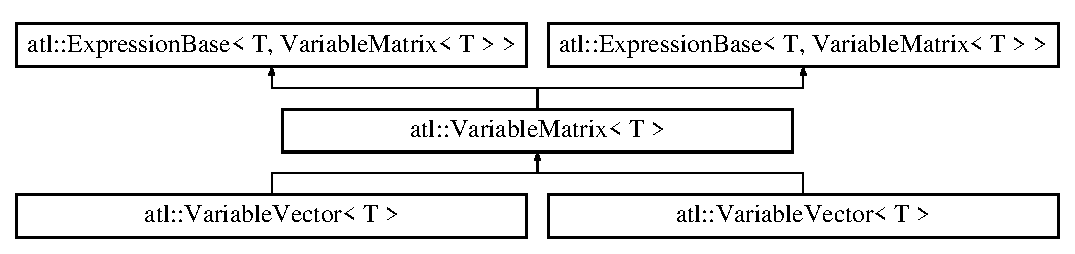
\includegraphics[height=2.968198cm]{structatl_1_1_variable_matrix}
\end{center}
\end{figure}
\subsection*{Public Member Functions}
\begin{DoxyCompactItemize}
\item 
\hypertarget{structatl_1_1_variable_matrix_af656ffe0e832bf82e4d4246c4fae3058}{{\bfseries Variable\+Matrix} (size\+\_\+t rows=0, size\+\_\+t columns=1, T initial\+\_\+value=static\+\_\+cast$<$ T $>$(0.\+0))}\label{structatl_1_1_variable_matrix_af656ffe0e832bf82e4d4246c4fae3058}

\item 
\hypertarget{structatl_1_1_variable_matrix_ac83b3849f3f3e984819716b69596fe63}{\hyperlink{structatl_1_1_variable_matrix}{Variable\+Matrix} \& {\bfseries operator=} (const T \&value)}\label{structatl_1_1_variable_matrix_ac83b3849f3f3e984819716b69596fe63}

\item 
\hypertarget{structatl_1_1_variable_matrix_adfaf4a2ae2591236e5df9d96aaa19783}{{\footnotesize template$<$class A $>$ }\\\hyperlink{structatl_1_1_variable_matrix}{Variable\+Matrix} \& {\bfseries operator=} (const \hyperlink{structatl_1_1_expression_base}{Expression\+Base}$<$ T, A $>$ \&exp)}\label{structatl_1_1_variable_matrix_adfaf4a2ae2591236e5df9d96aaa19783}

\item 
\hypertarget{structatl_1_1_variable_matrix_a042ca0e4a046575dbe471fd107526bcb}{{\footnotesize template$<$class A $>$ }\\\hyperlink{structatl_1_1_variable_matrix}{Variable\+Matrix} \& {\bfseries Assign\+Concurrent} (const \hyperlink{structatl_1_1_expression_base}{Expression\+Base}$<$ T, A $>$ \&exp)}\label{structatl_1_1_variable_matrix_a042ca0e4a046575dbe471fd107526bcb}

\item 
\hypertarget{structatl_1_1_variable_matrix_a467767c1d7a162b3ec0d56c85f05822e}{void {\bfseries Push\+Ids} (typename \hyperlink{structatl_1_1_stack_entry}{atl\+::\+Stack\+Entry}$<$ T $>$\+::vi\+\_\+storage \&ids) const }\label{structatl_1_1_variable_matrix_a467767c1d7a162b3ec0d56c85f05822e}

\item 
\hypertarget{structatl_1_1_variable_matrix_a87472f5b1f82f7b977d94fe9172e7d28}{void {\bfseries Push\+Ids} (typename \hyperlink{structatl_1_1_stack_entry}{atl\+::\+Stack\+Entry}$<$ T $>$\+::vi\+\_\+storage \&ids, size\+\_\+t i, size\+\_\+t j=0) const }\label{structatl_1_1_variable_matrix_a87472f5b1f82f7b977d94fe9172e7d28}

\item 
\hypertarget{structatl_1_1_variable_matrix_a949002e9718e5c89afa7566a92d92103}{\hyperlink{structatl_1_1_variable}{atl\+::\+Variable}$<$ T $>$ \& {\bfseries operator()} (size\+\_\+t i, size\+\_\+t j=0)}\label{structatl_1_1_variable_matrix_a949002e9718e5c89afa7566a92d92103}

\item 
\hypertarget{structatl_1_1_variable_matrix_a6d873cfa56fe801abb7a53b22d36f081}{const \hyperlink{structatl_1_1_variable}{atl\+::\+Variable}$<$ T $>$ \& {\bfseries operator()} (size\+\_\+t i, size\+\_\+t j=0) const }\label{structatl_1_1_variable_matrix_a6d873cfa56fe801abb7a53b22d36f081}

\item 
\hypertarget{structatl_1_1_variable_matrix_ad94d8c617309904428255343e7c0ba3e}{const T {\bfseries Get\+Value} () const }\label{structatl_1_1_variable_matrix_ad94d8c617309904428255343e7c0ba3e}

\item 
\hypertarget{structatl_1_1_variable_matrix_aadaa361a31a643b56c16dcaf912a4b45}{const T {\bfseries Get\+Value} (size\+\_\+t i, size\+\_\+t j=0) const }\label{structatl_1_1_variable_matrix_aadaa361a31a643b56c16dcaf912a4b45}

\item 
\hypertarget{structatl_1_1_variable_matrix_ad6587a3521473952b5034c189656fc89}{T {\bfseries Evaluate\+Derivative} (uint32\+\_\+t a) const }\label{structatl_1_1_variable_matrix_ad6587a3521473952b5034c189656fc89}

\item 
\hypertarget{structatl_1_1_variable_matrix_ad30a3eb8147e9c685e6f1d4c2c128e77}{T {\bfseries Evaluate\+Derivative} (uint32\+\_\+t a, uint32\+\_\+t b) const }\label{structatl_1_1_variable_matrix_ad30a3eb8147e9c685e6f1d4c2c128e77}

\item 
\hypertarget{structatl_1_1_variable_matrix_aa149ea3e1fd7dcfb90f41e6e3f847eb5}{T {\bfseries Evaluate\+Derivative} (uint32\+\_\+t x, uint32\+\_\+t y, uint32\+\_\+t z) const }\label{structatl_1_1_variable_matrix_aa149ea3e1fd7dcfb90f41e6e3f847eb5}

\item 
\hypertarget{structatl_1_1_variable_matrix_ab7747464b84e1c5e49642d19dadeda20}{T {\bfseries Evaluate\+Derivative} (uint32\+\_\+t a, size\+\_\+t i, size\+\_\+t j=0) const }\label{structatl_1_1_variable_matrix_ab7747464b84e1c5e49642d19dadeda20}

\item 
\hypertarget{structatl_1_1_variable_matrix_a1744bf3e4399c21f380de713fb5481da}{T {\bfseries Evaluate\+Derivative} (uint32\+\_\+t a, uint32\+\_\+t b, size\+\_\+t i, size\+\_\+t j=0) const }\label{structatl_1_1_variable_matrix_a1744bf3e4399c21f380de713fb5481da}

\item 
\hypertarget{structatl_1_1_variable_matrix_a2a1af09f111aed65d69a44651cb36ced}{T {\bfseries Evaluate\+Derivative} (uint32\+\_\+t x, uint32\+\_\+t y, uint32\+\_\+t z, size\+\_\+t i, size\+\_\+t j=0) const }\label{structatl_1_1_variable_matrix_a2a1af09f111aed65d69a44651cb36ced}

\item 
\hypertarget{structatl_1_1_variable_matrix_aa23031ddb3becdaa0c36717bd9b44f5c}{size\+\_\+t {\bfseries Get\+Columns} () const }\label{structatl_1_1_variable_matrix_aa23031ddb3becdaa0c36717bd9b44f5c}

\item 
\hypertarget{structatl_1_1_variable_matrix_a256ec551bfd19efc13d89a9b993d992a}{size\+\_\+t {\bfseries Get\+Rows} () const }\label{structatl_1_1_variable_matrix_a256ec551bfd19efc13d89a9b993d992a}

\item 
\hypertarget{structatl_1_1_variable_matrix_ab08d56cb74dda075d1764865f3e8fd07}{bool {\bfseries Is\+Scalar} () const }\label{structatl_1_1_variable_matrix_ab08d56cb74dda075d1764865f3e8fd07}

\item 
\hyperlink{structatl_1_1_variable_matrix_af656ffe0e832bf82e4d4246c4fae3058}{Variable\+Matrix} (size\+\_\+t rows=0, size\+\_\+t columns=1, T initial\+\_\+value=static\+\_\+cast$<$ T $>$(0.\+0))
\item 
\hyperlink{structatl_1_1_variable_matrix}{Variable\+Matrix} \& \hyperlink{structatl_1_1_variable_matrix_ac83b3849f3f3e984819716b69596fe63}{operator=} (const T \&value)
\item 
{\footnotesize template$<$class A $>$ }\\\hyperlink{structatl_1_1_variable_matrix}{Variable\+Matrix} \& \hyperlink{structatl_1_1_variable_matrix_adfaf4a2ae2591236e5df9d96aaa19783}{operator=} (const \hyperlink{structatl_1_1_expression_base}{Expression\+Base}$<$ T, A $>$ \&exp)
\item 
{\footnotesize template$<$class A $>$ }\\\hyperlink{structatl_1_1_variable_matrix}{Variable\+Matrix} \& \hyperlink{structatl_1_1_variable_matrix_a042ca0e4a046575dbe471fd107526bcb}{Assign\+Concurrent} (const \hyperlink{structatl_1_1_expression_base}{Expression\+Base}$<$ T, A $>$ \&exp)
\item 
void \hyperlink{structatl_1_1_variable_matrix_a467767c1d7a162b3ec0d56c85f05822e}{Push\+Ids} (typename \hyperlink{structatl_1_1_stack_entry}{atl\+::\+Stack\+Entry}$<$ T $>$\+::vi\+\_\+storage \&ids) const 
\item 
void \hyperlink{structatl_1_1_variable_matrix_a87472f5b1f82f7b977d94fe9172e7d28}{Push\+Ids} (typename \hyperlink{structatl_1_1_stack_entry}{atl\+::\+Stack\+Entry}$<$ T $>$\+::vi\+\_\+storage \&ids, size\+\_\+t i, size\+\_\+t j=0) const 
\item 
\hyperlink{structatl_1_1_variable}{atl\+::\+Variable}$<$ T $>$ \& \hyperlink{structatl_1_1_variable_matrix_a949002e9718e5c89afa7566a92d92103}{operator()} (size\+\_\+t i, size\+\_\+t j=0)
\item 
const \hyperlink{structatl_1_1_variable}{atl\+::\+Variable}$<$ T $>$ \& \hyperlink{structatl_1_1_variable_matrix_a6d873cfa56fe801abb7a53b22d36f081}{operator()} (size\+\_\+t i, size\+\_\+t j=0) const 
\item 
const T \hyperlink{structatl_1_1_variable_matrix_ad94d8c617309904428255343e7c0ba3e}{Get\+Value} () const 
\item 
const T \hyperlink{structatl_1_1_variable_matrix_aadaa361a31a643b56c16dcaf912a4b45}{Get\+Value} (size\+\_\+t i, size\+\_\+t j=0) const 
\item 
bool \hyperlink{structatl_1_1_variable_matrix_a5dd3b0548d277b4643f4953d9ec200f2}{Is\+Nonlinear} () const 
\item 
T \hyperlink{structatl_1_1_variable_matrix_a2892998b53099125116cb6fc92ae2eef}{Evaluate\+Derivative} (uint32\+\_\+t x) const 
\item 
T \hyperlink{structatl_1_1_variable_matrix_af9d21b0cd88c29b65e48dd47419fd1f5}{Evaluate\+Derivative} (uint32\+\_\+t x, uint32\+\_\+t y) const 
\item 
T \hyperlink{structatl_1_1_variable_matrix_aa149ea3e1fd7dcfb90f41e6e3f847eb5}{Evaluate\+Derivative} (uint32\+\_\+t x, uint32\+\_\+t y, uint32\+\_\+t z) const 
\item 
T \hyperlink{structatl_1_1_variable_matrix_a9bed2ae3ac39bb9574fcdbdff3badf47}{Evaluate\+Derivative} (uint32\+\_\+t x, size\+\_\+t i, size\+\_\+t j=0) const 
\item 
T \hyperlink{structatl_1_1_variable_matrix_a4c084e102edd1acfdd1a6211bfa5f312}{Evaluate\+Derivative} (uint32\+\_\+t x, uint32\+\_\+t y, size\+\_\+t i, size\+\_\+t j=0) const 
\item 
T \hyperlink{structatl_1_1_variable_matrix_a2a1af09f111aed65d69a44651cb36ced}{Evaluate\+Derivative} (uint32\+\_\+t x, uint32\+\_\+t y, uint32\+\_\+t z, size\+\_\+t i, size\+\_\+t j=0) const 
\item 
size\+\_\+t \hyperlink{structatl_1_1_variable_matrix_aa23031ddb3becdaa0c36717bd9b44f5c}{Get\+Columns} () const 
\item 
size\+\_\+t \hyperlink{structatl_1_1_variable_matrix_a256ec551bfd19efc13d89a9b993d992a}{Get\+Rows} () const 
\item 
bool \hyperlink{structatl_1_1_variable_matrix_ab08d56cb74dda075d1764865f3e8fd07}{Is\+Scalar} () const 
\end{DoxyCompactItemize}
\subsection*{Public Attributes}
\begin{DoxyCompactItemize}
\item 
\hypertarget{structatl_1_1_variable_matrix_ae33cc85e892a1e8622b22f39a86b1dd9}{size\+\_\+t {\bfseries rows}}\label{structatl_1_1_variable_matrix_ae33cc85e892a1e8622b22f39a86b1dd9}

\item 
\hypertarget{structatl_1_1_variable_matrix_a88ba4cdd712df04884811e9c43c25956}{size\+\_\+t {\bfseries columns}}\label{structatl_1_1_variable_matrix_a88ba4cdd712df04884811e9c43c25956}

\item 
\hypertarget{structatl_1_1_variable_matrix_ab005ef7a62ac08c6d4c2afc0813b0ddb}{std\+::vector$<$ \hyperlink{structatl_1_1_variable}{atl\+::\+Variable}$<$ T $>$\\*
, \hyperlink{structatl_1_1clfallocator}{atl\+::clfallocator}\\*
$<$ \hyperlink{structatl_1_1_variable}{atl\+::\+Variable}$<$ T $>$ $>$ $>$ {\bfseries data\+\_\+m}}\label{structatl_1_1_variable_matrix_ab005ef7a62ac08c6d4c2afc0813b0ddb}

\end{DoxyCompactItemize}


\subsection{Detailed Description}
\subsubsection*{template$<$typename T$>$struct atl\+::\+Variable\+Matrix$<$ T $>$}

Matrix of \hyperlink{structatl_1_1_variable}{Variable} types. 

\subsection{Constructor \& Destructor Documentation}
\hypertarget{structatl_1_1_variable_matrix_af656ffe0e832bf82e4d4246c4fae3058}{\index{atl\+::\+Variable\+Matrix@{atl\+::\+Variable\+Matrix}!Variable\+Matrix@{Variable\+Matrix}}
\index{Variable\+Matrix@{Variable\+Matrix}!atl\+::\+Variable\+Matrix@{atl\+::\+Variable\+Matrix}}
\subsubsection[{Variable\+Matrix}]{\setlength{\rightskip}{0pt plus 5cm}template$<$typename T$>$ {\bf atl\+::\+Variable\+Matrix}$<$ T $>$\+::{\bf Variable\+Matrix} (
\begin{DoxyParamCaption}
\item[{size\+\_\+t}]{rows = {\ttfamily 0}, }
\item[{size\+\_\+t}]{columns = {\ttfamily 1}, }
\item[{T}]{initial\+\_\+value = {\ttfamily static\+\_\+cast$<$T$>$~(0.0)}}
\end{DoxyParamCaption}
)\hspace{0.3cm}{\ttfamily [inline]}}}\label{structatl_1_1_variable_matrix_af656ffe0e832bf82e4d4246c4fae3058}
Constructor.


\begin{DoxyParams}{Parameters}
{\em rows} & \\
\hline
{\em columns} & \\
\hline
{\em initial\+\_\+value} & \\
\hline
\end{DoxyParams}


\subsection{Member Function Documentation}
\hypertarget{structatl_1_1_variable_matrix_a042ca0e4a046575dbe471fd107526bcb}{\index{atl\+::\+Variable\+Matrix@{atl\+::\+Variable\+Matrix}!Assign\+Concurrent@{Assign\+Concurrent}}
\index{Assign\+Concurrent@{Assign\+Concurrent}!atl\+::\+Variable\+Matrix@{atl\+::\+Variable\+Matrix}}
\subsubsection[{Assign\+Concurrent}]{\setlength{\rightskip}{0pt plus 5cm}template$<$typename T$>$ template$<$class A $>$ {\bf Variable\+Matrix}\& {\bf atl\+::\+Variable\+Matrix}$<$ T $>$\+::Assign\+Concurrent (
\begin{DoxyParamCaption}
\item[{const {\bf Expression\+Base}$<$ T, A $>$ \&}]{exp}
\end{DoxyParamCaption}
)\hspace{0.3cm}{\ttfamily [inline]}}}\label{structatl_1_1_variable_matrix_a042ca0e4a046575dbe471fd107526bcb}
Assignment function for concurrent assignment. This function guarantees proper tape recording by reserving a block of entries from the \hyperlink{classatl_1_1_tape}{Tape} and allocating among threads accordingly. Each thread receives a reference to exp and its range of \hyperlink{classatl_1_1_tape}{Tape} entries.


\begin{DoxyParams}{Parameters}
{\em exp} & \\
\hline
\end{DoxyParams}
\begin{DoxyReturn}{Returns}

\end{DoxyReturn}
\hypertarget{structatl_1_1_variable_matrix_a2892998b53099125116cb6fc92ae2eef}{\index{atl\+::\+Variable\+Matrix@{atl\+::\+Variable\+Matrix}!Evaluate\+Derivative@{Evaluate\+Derivative}}
\index{Evaluate\+Derivative@{Evaluate\+Derivative}!atl\+::\+Variable\+Matrix@{atl\+::\+Variable\+Matrix}}
\subsubsection[{Evaluate\+Derivative}]{\setlength{\rightskip}{0pt plus 5cm}template$<$typename T$>$ T {\bf atl\+::\+Variable\+Matrix}$<$ T $>$\+::Evaluate\+Derivative (
\begin{DoxyParamCaption}
\item[{uint32\+\_\+t}]{x}
\end{DoxyParamCaption}
) const\hspace{0.3cm}{\ttfamily [inline]}}}\label{structatl_1_1_variable_matrix_a2892998b53099125116cb6fc92ae2eef}
throws std\+::invalid\+\_\+argument \begin{DoxyReturn}{Returns}

\end{DoxyReturn}
\hypertarget{structatl_1_1_variable_matrix_af9d21b0cd88c29b65e48dd47419fd1f5}{\index{atl\+::\+Variable\+Matrix@{atl\+::\+Variable\+Matrix}!Evaluate\+Derivative@{Evaluate\+Derivative}}
\index{Evaluate\+Derivative@{Evaluate\+Derivative}!atl\+::\+Variable\+Matrix@{atl\+::\+Variable\+Matrix}}
\subsubsection[{Evaluate\+Derivative}]{\setlength{\rightskip}{0pt plus 5cm}template$<$typename T$>$ T {\bf atl\+::\+Variable\+Matrix}$<$ T $>$\+::Evaluate\+Derivative (
\begin{DoxyParamCaption}
\item[{uint32\+\_\+t}]{x, }
\item[{uint32\+\_\+t}]{y}
\end{DoxyParamCaption}
) const\hspace{0.3cm}{\ttfamily [inline]}}}\label{structatl_1_1_variable_matrix_af9d21b0cd88c29b65e48dd47419fd1f5}
throws std\+::invalid\+\_\+argument \begin{DoxyReturn}{Returns}

\end{DoxyReturn}
\hypertarget{structatl_1_1_variable_matrix_aa149ea3e1fd7dcfb90f41e6e3f847eb5}{\index{atl\+::\+Variable\+Matrix@{atl\+::\+Variable\+Matrix}!Evaluate\+Derivative@{Evaluate\+Derivative}}
\index{Evaluate\+Derivative@{Evaluate\+Derivative}!atl\+::\+Variable\+Matrix@{atl\+::\+Variable\+Matrix}}
\subsubsection[{Evaluate\+Derivative}]{\setlength{\rightskip}{0pt plus 5cm}template$<$typename T$>$ T {\bf atl\+::\+Variable\+Matrix}$<$ T $>$\+::Evaluate\+Derivative (
\begin{DoxyParamCaption}
\item[{uint32\+\_\+t}]{x, }
\item[{uint32\+\_\+t}]{y, }
\item[{uint32\+\_\+t}]{z}
\end{DoxyParamCaption}
) const\hspace{0.3cm}{\ttfamily [inline]}}}\label{structatl_1_1_variable_matrix_aa149ea3e1fd7dcfb90f41e6e3f847eb5}
throws std\+::invalid\+\_\+argument \begin{DoxyReturn}{Returns}

\end{DoxyReturn}
\hypertarget{structatl_1_1_variable_matrix_a9bed2ae3ac39bb9574fcdbdff3badf47}{\index{atl\+::\+Variable\+Matrix@{atl\+::\+Variable\+Matrix}!Evaluate\+Derivative@{Evaluate\+Derivative}}
\index{Evaluate\+Derivative@{Evaluate\+Derivative}!atl\+::\+Variable\+Matrix@{atl\+::\+Variable\+Matrix}}
\subsubsection[{Evaluate\+Derivative}]{\setlength{\rightskip}{0pt plus 5cm}template$<$typename T$>$ T {\bf atl\+::\+Variable\+Matrix}$<$ T $>$\+::Evaluate\+Derivative (
\begin{DoxyParamCaption}
\item[{uint32\+\_\+t}]{x, }
\item[{size\+\_\+t}]{i, }
\item[{size\+\_\+t}]{j = {\ttfamily 0}}
\end{DoxyParamCaption}
) const\hspace{0.3cm}{\ttfamily [inline]}}}\label{structatl_1_1_variable_matrix_a9bed2ae3ac39bb9574fcdbdff3badf47}
Evaluates the first-\/order derivative at index \{i,j\}.

Returns 1 if index \{i,j\} is equal to x, else it returns 0.


\begin{DoxyParams}{Parameters}
{\em x} & \\
\hline
{\em i} & \\
\hline
{\em j} & \\
\hline
\end{DoxyParams}
\begin{DoxyReturn}{Returns}

\end{DoxyReturn}
\hypertarget{structatl_1_1_variable_matrix_a4c084e102edd1acfdd1a6211bfa5f312}{\index{atl\+::\+Variable\+Matrix@{atl\+::\+Variable\+Matrix}!Evaluate\+Derivative@{Evaluate\+Derivative}}
\index{Evaluate\+Derivative@{Evaluate\+Derivative}!atl\+::\+Variable\+Matrix@{atl\+::\+Variable\+Matrix}}
\subsubsection[{Evaluate\+Derivative}]{\setlength{\rightskip}{0pt plus 5cm}template$<$typename T$>$ T {\bf atl\+::\+Variable\+Matrix}$<$ T $>$\+::Evaluate\+Derivative (
\begin{DoxyParamCaption}
\item[{uint32\+\_\+t}]{x, }
\item[{uint32\+\_\+t}]{y, }
\item[{size\+\_\+t}]{i, }
\item[{size\+\_\+t}]{j = {\ttfamily 0}}
\end{DoxyParamCaption}
) const\hspace{0.3cm}{\ttfamily [inline]}}}\label{structatl_1_1_variable_matrix_a4c084e102edd1acfdd1a6211bfa5f312}
Returns 0.


\begin{DoxyParams}{Parameters}
{\em x} & \\
\hline
{\em x} & \\
\hline
{\em i} & \\
\hline
{\em j} & \\
\hline
\end{DoxyParams}
\begin{DoxyReturn}{Returns}

\end{DoxyReturn}
\hypertarget{structatl_1_1_variable_matrix_a2a1af09f111aed65d69a44651cb36ced}{\index{atl\+::\+Variable\+Matrix@{atl\+::\+Variable\+Matrix}!Evaluate\+Derivative@{Evaluate\+Derivative}}
\index{Evaluate\+Derivative@{Evaluate\+Derivative}!atl\+::\+Variable\+Matrix@{atl\+::\+Variable\+Matrix}}
\subsubsection[{Evaluate\+Derivative}]{\setlength{\rightskip}{0pt plus 5cm}template$<$typename T$>$ T {\bf atl\+::\+Variable\+Matrix}$<$ T $>$\+::Evaluate\+Derivative (
\begin{DoxyParamCaption}
\item[{uint32\+\_\+t}]{x, }
\item[{uint32\+\_\+t}]{y, }
\item[{uint32\+\_\+t}]{z, }
\item[{size\+\_\+t}]{i, }
\item[{size\+\_\+t}]{j = {\ttfamily 0}}
\end{DoxyParamCaption}
) const\hspace{0.3cm}{\ttfamily [inline]}}}\label{structatl_1_1_variable_matrix_a2a1af09f111aed65d69a44651cb36ced}
Returns 0.


\begin{DoxyParams}{Parameters}
{\em x} & \\
\hline
{\em y} & \\
\hline
{\em z} & \\
\hline
{\em i} & \\
\hline
{\em j} & \\
\hline
\end{DoxyParams}
\begin{DoxyReturn}{Returns}

\end{DoxyReturn}
\hypertarget{structatl_1_1_variable_matrix_aa23031ddb3becdaa0c36717bd9b44f5c}{\index{atl\+::\+Variable\+Matrix@{atl\+::\+Variable\+Matrix}!Get\+Columns@{Get\+Columns}}
\index{Get\+Columns@{Get\+Columns}!atl\+::\+Variable\+Matrix@{atl\+::\+Variable\+Matrix}}
\subsubsection[{Get\+Columns}]{\setlength{\rightskip}{0pt plus 5cm}template$<$typename T$>$ size\+\_\+t {\bf atl\+::\+Variable\+Matrix}$<$ T $>$\+::Get\+Columns (
\begin{DoxyParamCaption}
{}
\end{DoxyParamCaption}
) const\hspace{0.3cm}{\ttfamily [inline]}}}\label{structatl_1_1_variable_matrix_aa23031ddb3becdaa0c36717bd9b44f5c}
Returns the number of columns.

\begin{DoxyReturn}{Returns}

\end{DoxyReturn}
\hypertarget{structatl_1_1_variable_matrix_a256ec551bfd19efc13d89a9b993d992a}{\index{atl\+::\+Variable\+Matrix@{atl\+::\+Variable\+Matrix}!Get\+Rows@{Get\+Rows}}
\index{Get\+Rows@{Get\+Rows}!atl\+::\+Variable\+Matrix@{atl\+::\+Variable\+Matrix}}
\subsubsection[{Get\+Rows}]{\setlength{\rightskip}{0pt plus 5cm}template$<$typename T$>$ size\+\_\+t {\bf atl\+::\+Variable\+Matrix}$<$ T $>$\+::Get\+Rows (
\begin{DoxyParamCaption}
{}
\end{DoxyParamCaption}
) const\hspace{0.3cm}{\ttfamily [inline]}}}\label{structatl_1_1_variable_matrix_a256ec551bfd19efc13d89a9b993d992a}
Returns the number of rows.

\begin{DoxyReturn}{Returns}

\end{DoxyReturn}
\hypertarget{structatl_1_1_variable_matrix_ad94d8c617309904428255343e7c0ba3e}{\index{atl\+::\+Variable\+Matrix@{atl\+::\+Variable\+Matrix}!Get\+Value@{Get\+Value}}
\index{Get\+Value@{Get\+Value}!atl\+::\+Variable\+Matrix@{atl\+::\+Variable\+Matrix}}
\subsubsection[{Get\+Value}]{\setlength{\rightskip}{0pt plus 5cm}template$<$typename T$>$ const T {\bf atl\+::\+Variable\+Matrix}$<$ T $>$\+::Get\+Value (
\begin{DoxyParamCaption}
{}
\end{DoxyParamCaption}
) const\hspace{0.3cm}{\ttfamily [inline]}}}\label{structatl_1_1_variable_matrix_ad94d8c617309904428255343e7c0ba3e}
throws std\+::invalid\+\_\+argument \begin{DoxyReturn}{Returns}

\end{DoxyReturn}
\hypertarget{structatl_1_1_variable_matrix_aadaa361a31a643b56c16dcaf912a4b45}{\index{atl\+::\+Variable\+Matrix@{atl\+::\+Variable\+Matrix}!Get\+Value@{Get\+Value}}
\index{Get\+Value@{Get\+Value}!atl\+::\+Variable\+Matrix@{atl\+::\+Variable\+Matrix}}
\subsubsection[{Get\+Value}]{\setlength{\rightskip}{0pt plus 5cm}template$<$typename T$>$ const T {\bf atl\+::\+Variable\+Matrix}$<$ T $>$\+::Get\+Value (
\begin{DoxyParamCaption}
\item[{size\+\_\+t}]{i, }
\item[{size\+\_\+t}]{j = {\ttfamily 0}}
\end{DoxyParamCaption}
) const\hspace{0.3cm}{\ttfamily [inline]}}}\label{structatl_1_1_variable_matrix_aadaa361a31a643b56c16dcaf912a4b45}
Returns the real value at index \{i,j\}. 
\begin{DoxyParams}{Parameters}
{\em i} & \\
\hline
{\em j} & \\
\hline
\end{DoxyParams}
\begin{DoxyReturn}{Returns}

\end{DoxyReturn}
\hypertarget{structatl_1_1_variable_matrix_a5dd3b0548d277b4643f4953d9ec200f2}{\index{atl\+::\+Variable\+Matrix@{atl\+::\+Variable\+Matrix}!Is\+Nonlinear@{Is\+Nonlinear}}
\index{Is\+Nonlinear@{Is\+Nonlinear}!atl\+::\+Variable\+Matrix@{atl\+::\+Variable\+Matrix}}
\subsubsection[{Is\+Nonlinear}]{\setlength{\rightskip}{0pt plus 5cm}template$<$typename T$>$ bool {\bf atl\+::\+Variable\+Matrix}$<$ T $>$\+::Is\+Nonlinear (
\begin{DoxyParamCaption}
{}
\end{DoxyParamCaption}
) const\hspace{0.3cm}{\ttfamily [inline]}}}\label{structatl_1_1_variable_matrix_a5dd3b0548d277b4643f4953d9ec200f2}
Returns false.

\begin{DoxyReturn}{Returns}

\end{DoxyReturn}
\hypertarget{structatl_1_1_variable_matrix_ab08d56cb74dda075d1764865f3e8fd07}{\index{atl\+::\+Variable\+Matrix@{atl\+::\+Variable\+Matrix}!Is\+Scalar@{Is\+Scalar}}
\index{Is\+Scalar@{Is\+Scalar}!atl\+::\+Variable\+Matrix@{atl\+::\+Variable\+Matrix}}
\subsubsection[{Is\+Scalar}]{\setlength{\rightskip}{0pt plus 5cm}template$<$typename T$>$ bool {\bf atl\+::\+Variable\+Matrix}$<$ T $>$\+::Is\+Scalar (
\begin{DoxyParamCaption}
{}
\end{DoxyParamCaption}
) const\hspace{0.3cm}{\ttfamily [inline]}}}\label{structatl_1_1_variable_matrix_ab08d56cb74dda075d1764865f3e8fd07}
Returns false. \hypertarget{structatl_1_1_variable_matrix_a949002e9718e5c89afa7566a92d92103}{\index{atl\+::\+Variable\+Matrix@{atl\+::\+Variable\+Matrix}!operator()@{operator()}}
\index{operator()@{operator()}!atl\+::\+Variable\+Matrix@{atl\+::\+Variable\+Matrix}}
\subsubsection[{operator()}]{\setlength{\rightskip}{0pt plus 5cm}template$<$typename T$>$ {\bf atl\+::\+Variable}$<$T$>$\& {\bf atl\+::\+Variable\+Matrix}$<$ T $>$\+::operator() (
\begin{DoxyParamCaption}
\item[{size\+\_\+t}]{i, }
\item[{size\+\_\+t}]{j = {\ttfamily 0}}
\end{DoxyParamCaption}
)\hspace{0.3cm}{\ttfamily [inline]}}}\label{structatl_1_1_variable_matrix_a949002e9718e5c89afa7566a92d92103}

\begin{DoxyParams}{Parameters}
{\em i} & \\
\hline
{\em j} & \\
\hline
\end{DoxyParams}
\begin{DoxyReturn}{Returns}

\end{DoxyReturn}
\hypertarget{structatl_1_1_variable_matrix_a6d873cfa56fe801abb7a53b22d36f081}{\index{atl\+::\+Variable\+Matrix@{atl\+::\+Variable\+Matrix}!operator()@{operator()}}
\index{operator()@{operator()}!atl\+::\+Variable\+Matrix@{atl\+::\+Variable\+Matrix}}
\subsubsection[{operator()}]{\setlength{\rightskip}{0pt plus 5cm}template$<$typename T$>$ const {\bf atl\+::\+Variable}$<$T$>$\& {\bf atl\+::\+Variable\+Matrix}$<$ T $>$\+::operator() (
\begin{DoxyParamCaption}
\item[{size\+\_\+t}]{i, }
\item[{size\+\_\+t}]{j = {\ttfamily 0}}
\end{DoxyParamCaption}
) const\hspace{0.3cm}{\ttfamily [inline]}}}\label{structatl_1_1_variable_matrix_a6d873cfa56fe801abb7a53b22d36f081}

\begin{DoxyParams}{Parameters}
{\em i} & \\
\hline
{\em j} & \\
\hline
\end{DoxyParams}
\begin{DoxyReturn}{Returns}

\end{DoxyReturn}
\hypertarget{structatl_1_1_variable_matrix_ac83b3849f3f3e984819716b69596fe63}{\index{atl\+::\+Variable\+Matrix@{atl\+::\+Variable\+Matrix}!operator=@{operator=}}
\index{operator=@{operator=}!atl\+::\+Variable\+Matrix@{atl\+::\+Variable\+Matrix}}
\subsubsection[{operator=}]{\setlength{\rightskip}{0pt plus 5cm}template$<$typename T$>$ {\bf Variable\+Matrix}\& {\bf atl\+::\+Variable\+Matrix}$<$ T $>$\+::operator= (
\begin{DoxyParamCaption}
\item[{const T \&}]{value}
\end{DoxyParamCaption}
)\hspace{0.3cm}{\ttfamily [inline]}}}\label{structatl_1_1_variable_matrix_ac83b3849f3f3e984819716b69596fe63}
Assignment operator. Sets all entries to value. 
\begin{DoxyParams}{Parameters}
{\em value} & \\
\hline
\end{DoxyParams}
\begin{DoxyReturn}{Returns}

\end{DoxyReturn}
\hypertarget{structatl_1_1_variable_matrix_adfaf4a2ae2591236e5df9d96aaa19783}{\index{atl\+::\+Variable\+Matrix@{atl\+::\+Variable\+Matrix}!operator=@{operator=}}
\index{operator=@{operator=}!atl\+::\+Variable\+Matrix@{atl\+::\+Variable\+Matrix}}
\subsubsection[{operator=}]{\setlength{\rightskip}{0pt plus 5cm}template$<$typename T$>$ template$<$class A $>$ {\bf Variable\+Matrix}\& {\bf atl\+::\+Variable\+Matrix}$<$ T $>$\+::operator= (
\begin{DoxyParamCaption}
\item[{const {\bf Expression\+Base}$<$ T, A $>$ \&}]{exp}
\end{DoxyParamCaption}
)\hspace{0.3cm}{\ttfamily [inline]}}}\label{structatl_1_1_variable_matrix_adfaf4a2ae2591236e5df9d96aaa19783}
Assignment operator for expression template types.


\begin{DoxyParams}{Parameters}
{\em exp} & \\
\hline
\end{DoxyParams}
\begin{DoxyReturn}{Returns}

\end{DoxyReturn}
\hypertarget{structatl_1_1_variable_matrix_a467767c1d7a162b3ec0d56c85f05822e}{\index{atl\+::\+Variable\+Matrix@{atl\+::\+Variable\+Matrix}!Push\+Ids@{Push\+Ids}}
\index{Push\+Ids@{Push\+Ids}!atl\+::\+Variable\+Matrix@{atl\+::\+Variable\+Matrix}}
\subsubsection[{Push\+Ids}]{\setlength{\rightskip}{0pt plus 5cm}template$<$typename T$>$ void {\bf atl\+::\+Variable\+Matrix}$<$ T $>$\+::Push\+Ids (
\begin{DoxyParamCaption}
\item[{typename {\bf atl\+::\+Stack\+Entry}$<$ T $>$\+::vi\+\_\+storage \&}]{ids}
\end{DoxyParamCaption}
) const\hspace{0.3cm}{\ttfamily [inline]}}}\label{structatl_1_1_variable_matrix_a467767c1d7a162b3ec0d56c85f05822e}
Push variable info into a set for index \{0,0\}..


\begin{DoxyParams}{Parameters}
{\em ids} & \\
\hline
\end{DoxyParams}
\hypertarget{structatl_1_1_variable_matrix_a87472f5b1f82f7b977d94fe9172e7d28}{\index{atl\+::\+Variable\+Matrix@{atl\+::\+Variable\+Matrix}!Push\+Ids@{Push\+Ids}}
\index{Push\+Ids@{Push\+Ids}!atl\+::\+Variable\+Matrix@{atl\+::\+Variable\+Matrix}}
\subsubsection[{Push\+Ids}]{\setlength{\rightskip}{0pt plus 5cm}template$<$typename T$>$ void {\bf atl\+::\+Variable\+Matrix}$<$ T $>$\+::Push\+Ids (
\begin{DoxyParamCaption}
\item[{typename {\bf atl\+::\+Stack\+Entry}$<$ T $>$\+::vi\+\_\+storage \&}]{ids, }
\item[{size\+\_\+t}]{i, }
\item[{size\+\_\+t}]{j = {\ttfamily 0}}
\end{DoxyParamCaption}
) const\hspace{0.3cm}{\ttfamily [inline]}}}\label{structatl_1_1_variable_matrix_a87472f5b1f82f7b977d94fe9172e7d28}
Push variable info into a set at index \{i,j\}.


\begin{DoxyParams}{Parameters}
{\em ids} & \\
\hline
\end{DoxyParams}


The documentation for this struct was generated from the following file\+:\begin{DoxyCompactItemize}
\item 
A\+T\+L2/Matrix.\+hpp\end{DoxyCompactItemize}

\hypertarget{structatl_1_1_variable_matrix_assign}{\section{atl\+:\+:Variable\+Matrix\+Assign$<$ T, A $>$ Struct Template Reference}
\label{structatl_1_1_variable_matrix_assign}\index{atl\+::\+Variable\+Matrix\+Assign$<$ T, A $>$@{atl\+::\+Variable\+Matrix\+Assign$<$ T, A $>$}}
}


{\ttfamily \#include $<$Matrix.\+hpp$>$}

\subsection*{Public Member Functions}
\begin{DoxyCompactItemize}
\item 
\hypertarget{structatl_1_1_variable_matrix_assign_a61af4c7cf5a2597116469d2e6c1281d0}{{\bfseries Variable\+Matrix\+Assign} (\hyperlink{structatl_1_1_variable_matrix}{atl\+::\+Variable\+Matrix}$<$ T $>$ \&m, std\+::vector$<$ T $>$ \&temp, size\+\_\+t index\+\_\+start, size\+\_\+t row\+\_\+start, size\+\_\+t row\+\_\+end, const \hyperlink{structatl_1_1_expression_base}{atl\+::\+Expression\+Base}$<$ T, A $>$ \&exp)}\label{structatl_1_1_variable_matrix_assign_a61af4c7cf5a2597116469d2e6c1281d0}

\item 
\hypertarget{structatl_1_1_variable_matrix_assign_a30b25b68b51d285bf7f7f373a0cbfdc2}{void {\bfseries operator()} ()}\label{structatl_1_1_variable_matrix_assign_a30b25b68b51d285bf7f7f373a0cbfdc2}

\item 
\hypertarget{structatl_1_1_variable_matrix_assign_a61af4c7cf5a2597116469d2e6c1281d0}{{\bfseries Variable\+Matrix\+Assign} (\hyperlink{structatl_1_1_variable_matrix}{atl\+::\+Variable\+Matrix}$<$ T $>$ \&m, std\+::vector$<$ T $>$ \&temp, size\+\_\+t index\+\_\+start, size\+\_\+t row\+\_\+start, size\+\_\+t row\+\_\+end, const \hyperlink{structatl_1_1_expression_base}{atl\+::\+Expression\+Base}$<$ T, A $>$ \&exp)}\label{structatl_1_1_variable_matrix_assign_a61af4c7cf5a2597116469d2e6c1281d0}

\item 
\hypertarget{structatl_1_1_variable_matrix_assign_a30b25b68b51d285bf7f7f373a0cbfdc2}{void {\bfseries operator()} ()}\label{structatl_1_1_variable_matrix_assign_a30b25b68b51d285bf7f7f373a0cbfdc2}

\end{DoxyCompactItemize}
\subsection*{Public Attributes}
\begin{DoxyCompactItemize}
\item 
\hypertarget{structatl_1_1_variable_matrix_assign_a280d897827baf4d5f8c9330c685fb30a}{\hyperlink{structatl_1_1_variable_matrix}{atl\+::\+Variable\+Matrix}$<$ T $>$ \& {\bfseries m}}\label{structatl_1_1_variable_matrix_assign_a280d897827baf4d5f8c9330c685fb30a}

\item 
\hypertarget{structatl_1_1_variable_matrix_assign_ae1bca9be06be10edda65be5481ccb492}{std\+::vector$<$ T $>$ \& {\bfseries temp}}\label{structatl_1_1_variable_matrix_assign_ae1bca9be06be10edda65be5481ccb492}

\item 
\hypertarget{structatl_1_1_variable_matrix_assign_a89ec828ff2ab980b96fa1009435f5368}{size\+\_\+t {\bfseries index\+\_\+start}}\label{structatl_1_1_variable_matrix_assign_a89ec828ff2ab980b96fa1009435f5368}

\item 
\hypertarget{structatl_1_1_variable_matrix_assign_af4c19cad478dc118dd518a58a2153c15}{size\+\_\+t {\bfseries row\+\_\+start}}\label{structatl_1_1_variable_matrix_assign_af4c19cad478dc118dd518a58a2153c15}

\item 
\hypertarget{structatl_1_1_variable_matrix_assign_a6512cb9f5edc097e7c8a847fb51a34a2}{size\+\_\+t {\bfseries row\+\_\+end}}\label{structatl_1_1_variable_matrix_assign_a6512cb9f5edc097e7c8a847fb51a34a2}

\item 
\hypertarget{structatl_1_1_variable_matrix_assign_a2295877822cacf14a56fb19393993640}{const \hyperlink{structatl_1_1_expression_base}{atl\+::\+Expression\+Base}$<$ T, A $>$ \& {\bfseries exp}}\label{structatl_1_1_variable_matrix_assign_a2295877822cacf14a56fb19393993640}

\end{DoxyCompactItemize}


\subsection{Detailed Description}
\subsubsection*{template$<$typename T, class A$>$struct atl\+::\+Variable\+Matrix\+Assign$<$ T, A $>$}

\hyperlink{structatl_1_1_variable_matrix}{Variable\+Matrix} assign functor used by Variable\+Matrix\+::\+Assign\+Concurrent

Passed to the \hyperlink{classatl_1_1_thread_pool}{Thread\+Pool}. 

The documentation for this struct was generated from the following file\+:\begin{DoxyCompactItemize}
\item 
A\+T\+L2/Matrix.\+hpp\end{DoxyCompactItemize}

\hypertarget{structatl_1_1_variable_vector}{\section{atl\+:\+:Variable\+Vector$<$ T $>$ Struct Template Reference}
\label{structatl_1_1_variable_vector}\index{atl\+::\+Variable\+Vector$<$ T $>$@{atl\+::\+Variable\+Vector$<$ T $>$}}
}


{\ttfamily \#include $<$Vector.\+hpp$>$}

Inheritance diagram for atl\+:\+:Variable\+Vector$<$ T $>$\+:\begin{figure}[H]
\begin{center}
\leavevmode
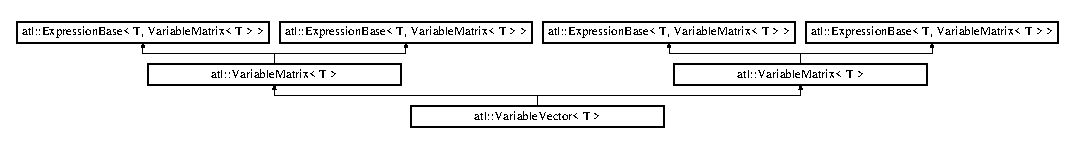
\includegraphics[height=1.484099cm]{structatl_1_1_variable_vector}
\end{center}
\end{figure}
\subsection*{Public Member Functions}
\begin{DoxyCompactItemize}
\item 
\hypertarget{structatl_1_1_variable_vector_ae69a156b19198f88af6383b33248e670}{{\bfseries Variable\+Vector} (size\+\_\+t rows=0)}\label{structatl_1_1_variable_vector_ae69a156b19198f88af6383b33248e670}

\item 
\hyperlink{structatl_1_1_variable_vector_a1328520eff96ab71f264146784d898ff}{Variable\+Vector} (size\+\_\+t columns=0)
\item 
void \hyperlink{structatl_1_1_variable_vector_a70470ad963a0126c2c7075c42348452d}{Set\+Size} (size\+\_\+t size)
\item 
size\+\_\+t \hyperlink{structatl_1_1_variable_vector_a5bd3fe223daeb5bf9d2358d93538a28c}{Get\+Size} ()
\item 
\hypertarget{structatl_1_1_variable_vector_aada89a21ba6184e7a1e3c6380cf9378c}{const std\+::string {\bfseries To\+Expression\+Template\+String} () const }\label{structatl_1_1_variable_vector_aada89a21ba6184e7a1e3c6380cf9378c}

\end{DoxyCompactItemize}
\subsection*{Additional Inherited Members}


\subsection{Detailed Description}
\subsubsection*{template$<$typename T$>$struct atl\+::\+Variable\+Vector$<$ T $>$}

\hyperlink{structatl_1_1_variable_vector}{Variable\+Vector} is a 1 x M \hyperlink{structatl_1_1_variable_matrix}{Variable\+Matrix}. 

\subsection{Constructor \& Destructor Documentation}
\hypertarget{structatl_1_1_variable_vector_a1328520eff96ab71f264146784d898ff}{\index{atl\+::\+Variable\+Vector@{atl\+::\+Variable\+Vector}!Variable\+Vector@{Variable\+Vector}}
\index{Variable\+Vector@{Variable\+Vector}!atl\+::\+Variable\+Vector@{atl\+::\+Variable\+Vector}}
\subsubsection[{Variable\+Vector}]{\setlength{\rightskip}{0pt plus 5cm}template$<$typename T $>$ {\bf atl\+::\+Variable\+Vector}$<$ T $>$\+::{\bf Variable\+Vector} (
\begin{DoxyParamCaption}
\item[{size\+\_\+t}]{columns = {\ttfamily 0}}
\end{DoxyParamCaption}
)\hspace{0.3cm}{\ttfamily [inline]}}}\label{structatl_1_1_variable_vector_a1328520eff96ab71f264146784d898ff}
Constructor. 
\begin{DoxyParams}{Parameters}
{\em columns} & \\
\hline
\end{DoxyParams}


\subsection{Member Function Documentation}
\hypertarget{structatl_1_1_variable_vector_a5bd3fe223daeb5bf9d2358d93538a28c}{\index{atl\+::\+Variable\+Vector@{atl\+::\+Variable\+Vector}!Get\+Size@{Get\+Size}}
\index{Get\+Size@{Get\+Size}!atl\+::\+Variable\+Vector@{atl\+::\+Variable\+Vector}}
\subsubsection[{Get\+Size}]{\setlength{\rightskip}{0pt plus 5cm}template$<$typename T $>$ size\+\_\+t {\bf atl\+::\+Variable\+Vector}$<$ T $>$\+::Get\+Size (
\begin{DoxyParamCaption}
{}
\end{DoxyParamCaption}
)\hspace{0.3cm}{\ttfamily [inline]}}}\label{structatl_1_1_variable_vector_a5bd3fe223daeb5bf9d2358d93538a28c}
Returns the size of this vector. \begin{DoxyReturn}{Returns}

\end{DoxyReturn}
\hypertarget{structatl_1_1_variable_vector_a70470ad963a0126c2c7075c42348452d}{\index{atl\+::\+Variable\+Vector@{atl\+::\+Variable\+Vector}!Set\+Size@{Set\+Size}}
\index{Set\+Size@{Set\+Size}!atl\+::\+Variable\+Vector@{atl\+::\+Variable\+Vector}}
\subsubsection[{Set\+Size}]{\setlength{\rightskip}{0pt plus 5cm}template$<$typename T $>$ void {\bf atl\+::\+Variable\+Vector}$<$ T $>$\+::Set\+Size (
\begin{DoxyParamCaption}
\item[{size\+\_\+t}]{size}
\end{DoxyParamCaption}
)\hspace{0.3cm}{\ttfamily [inline]}}}\label{structatl_1_1_variable_vector_a70470ad963a0126c2c7075c42348452d}
Sets the size of this vector.


\begin{DoxyParams}{Parameters}
{\em size} & \\
\hline
\end{DoxyParams}


The documentation for this struct was generated from the following file\+:\begin{DoxyCompactItemize}
\item 
A\+T\+L2/Vector.\+hpp\end{DoxyCompactItemize}

\hypertarget{classsimd_1_1vector2d}{\section{simd\+:\+:vector2d Class Reference}
\label{classsimd_1_1vector2d}\index{simd\+::vector2d@{simd\+::vector2d}}
}
Inheritance diagram for simd\+:\+:vector2d\+:\begin{figure}[H]
\begin{center}
\leavevmode
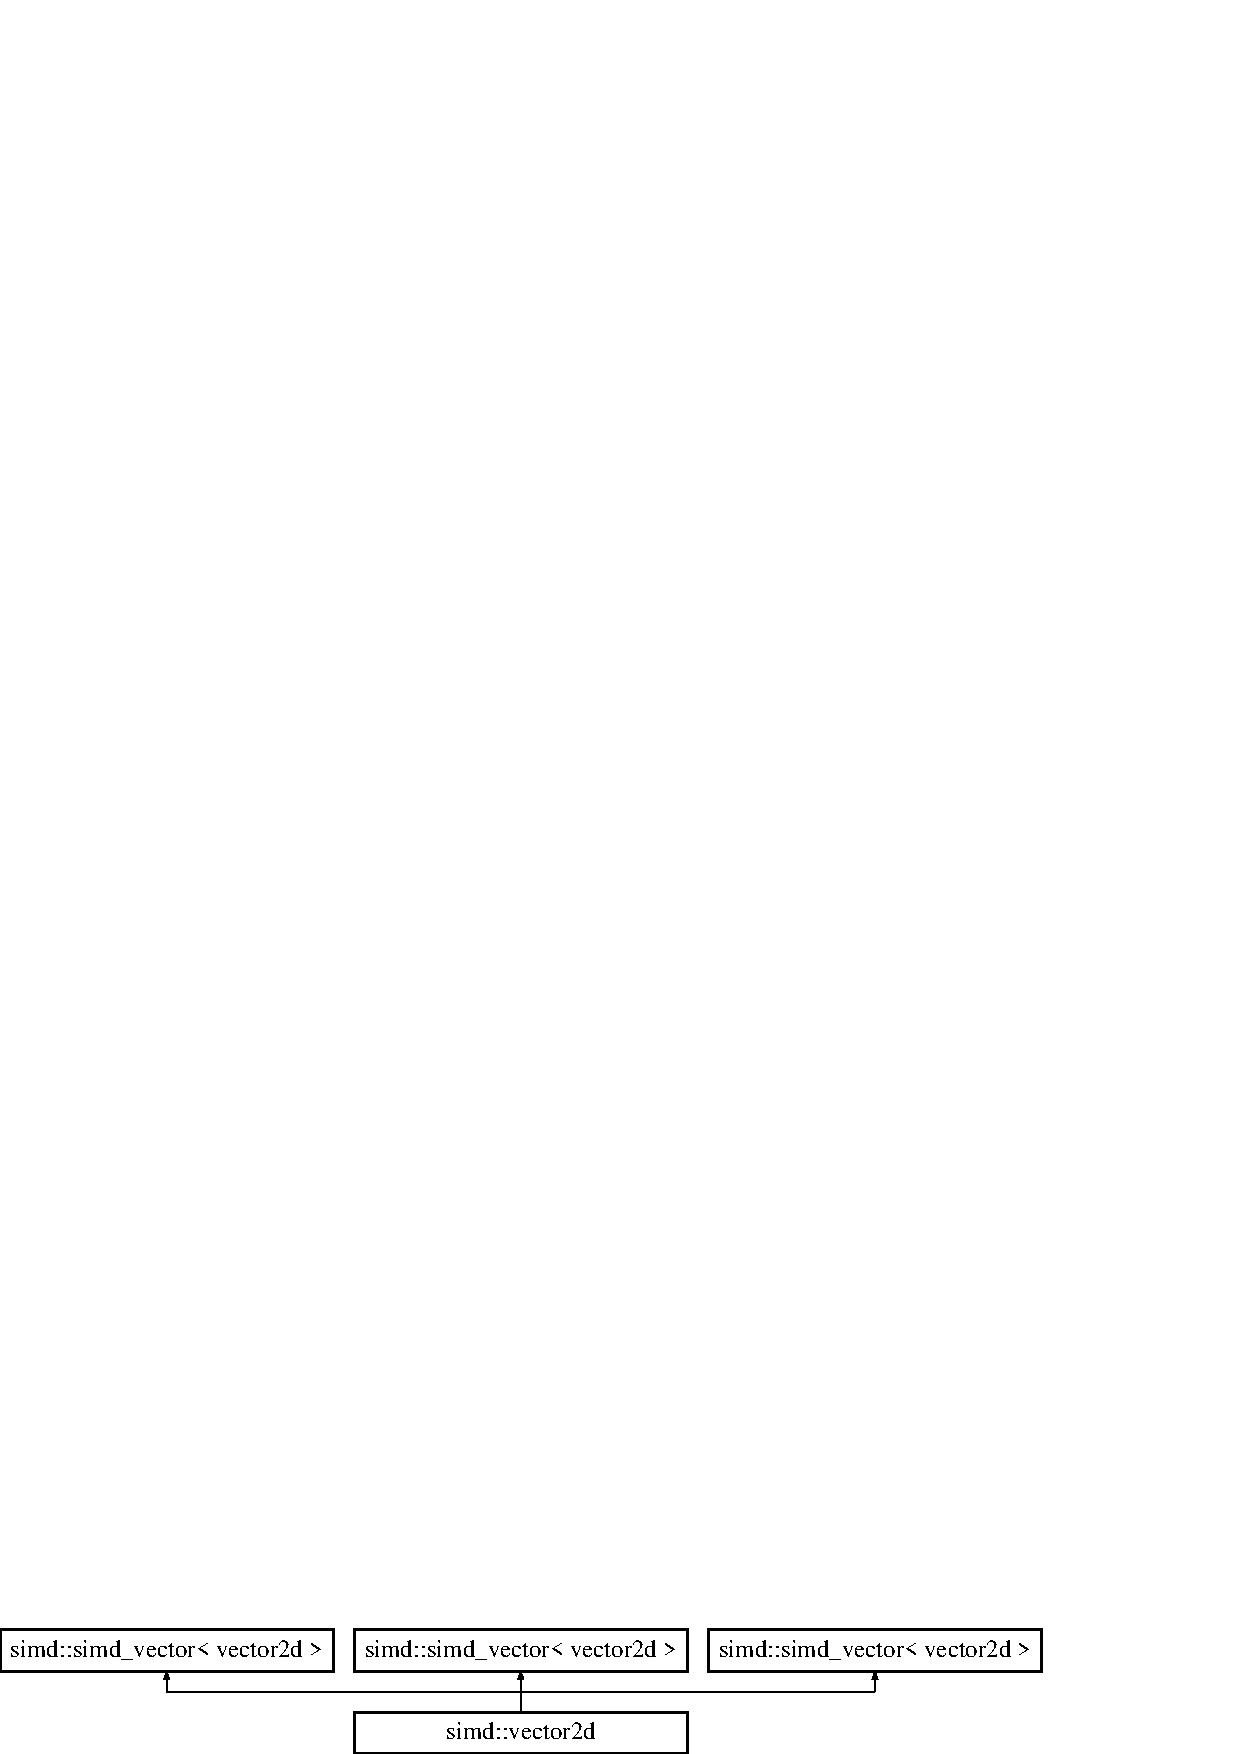
\includegraphics[height=1.934370cm]{classsimd_1_1vector2d}
\end{center}
\end{figure}
\subsection*{Public Member Functions}
\begin{DoxyCompactItemize}
\item 
\hypertarget{classsimd_1_1vector2d_a0e3a7eb244e825f7809aeca6c4015432}{{\bfseries vector2d} (double f)}\label{classsimd_1_1vector2d_a0e3a7eb244e825f7809aeca6c4015432}

\item 
\hypertarget{classsimd_1_1vector2d_a6bb8da073bec335551b009a92b7836e2}{{\bfseries vector2d} (double f0, double f1)}\label{classsimd_1_1vector2d_a6bb8da073bec335551b009a92b7836e2}

\item 
\hypertarget{classsimd_1_1vector2d_af5018df52051248f830d1d763733bd10}{{\bfseries vector2d} (const \+\_\+\+\_\+m128 \&rhs)}\label{classsimd_1_1vector2d_af5018df52051248f830d1d763733bd10}

\item 
\hypertarget{classsimd_1_1vector2d_ae0f759e6c5ad3236b64324883ef56362}{\hyperlink{classsimd_1_1vector2d}{vector2d} \& {\bfseries operator=} (const \+\_\+\+\_\+m128 \&rhs)}\label{classsimd_1_1vector2d_ae0f759e6c5ad3236b64324883ef56362}

\item 
\hypertarget{classsimd_1_1vector2d_a6d9c6d2fdcfd79caed0e0ca4ba6c4193}{{\bfseries operator \+\_\+\+\_\+m128} () const }\label{classsimd_1_1vector2d_a6d9c6d2fdcfd79caed0e0ca4ba6c4193}

\item 
\hypertarget{classsimd_1_1vector2d_a48343c3ce199a62c94a3628f4a9b8356}{\hyperlink{classsimd_1_1vector2d}{vector2d} \& {\bfseries load\+\_\+a} (const double $\ast$src)}\label{classsimd_1_1vector2d_a48343c3ce199a62c94a3628f4a9b8356}

\item 
\hypertarget{classsimd_1_1vector2d_aef41f161d484e293b5ed6f041cabc362}{\hyperlink{classsimd_1_1vector2d}{vector2d} \& {\bfseries load\+\_\+u} (const double $\ast$src)}\label{classsimd_1_1vector2d_aef41f161d484e293b5ed6f041cabc362}

\item 
\hypertarget{classsimd_1_1vector2d_ac7f65ddb8522ad00471574e00be3f0fe}{void {\bfseries store\+\_\+a} (double $\ast$dst) const }\label{classsimd_1_1vector2d_ac7f65ddb8522ad00471574e00be3f0fe}

\item 
\hypertarget{classsimd_1_1vector2d_a447736062fd8f0edd65db761cbe9a0fc}{void {\bfseries store\+\_\+u} (double $\ast$dst) const }\label{classsimd_1_1vector2d_a447736062fd8f0edd65db761cbe9a0fc}

\item 
\hypertarget{classsimd_1_1vector2d_a0e3a7eb244e825f7809aeca6c4015432}{{\bfseries vector2d} (double f)}\label{classsimd_1_1vector2d_a0e3a7eb244e825f7809aeca6c4015432}

\item 
\hypertarget{classsimd_1_1vector2d_a6bb8da073bec335551b009a92b7836e2}{{\bfseries vector2d} (double f0, double f1)}\label{classsimd_1_1vector2d_a6bb8da073bec335551b009a92b7836e2}

\item 
\hypertarget{classsimd_1_1vector2d_af5018df52051248f830d1d763733bd10}{{\bfseries vector2d} (const \+\_\+\+\_\+m128 \&rhs)}\label{classsimd_1_1vector2d_af5018df52051248f830d1d763733bd10}

\item 
\hypertarget{classsimd_1_1vector2d_ae0f759e6c5ad3236b64324883ef56362}{\hyperlink{classsimd_1_1vector2d}{vector2d} \& {\bfseries operator=} (const \+\_\+\+\_\+m128 \&rhs)}\label{classsimd_1_1vector2d_ae0f759e6c5ad3236b64324883ef56362}

\item 
\hypertarget{classsimd_1_1vector2d_a6d9c6d2fdcfd79caed0e0ca4ba6c4193}{{\bfseries operator \+\_\+\+\_\+m128} () const }\label{classsimd_1_1vector2d_a6d9c6d2fdcfd79caed0e0ca4ba6c4193}

\item 
\hypertarget{classsimd_1_1vector2d_a48343c3ce199a62c94a3628f4a9b8356}{\hyperlink{classsimd_1_1vector2d}{vector2d} \& {\bfseries load\+\_\+a} (const double $\ast$src)}\label{classsimd_1_1vector2d_a48343c3ce199a62c94a3628f4a9b8356}

\item 
\hypertarget{classsimd_1_1vector2d_aef41f161d484e293b5ed6f041cabc362}{\hyperlink{classsimd_1_1vector2d}{vector2d} \& {\bfseries load\+\_\+u} (const double $\ast$src)}\label{classsimd_1_1vector2d_aef41f161d484e293b5ed6f041cabc362}

\item 
\hypertarget{classsimd_1_1vector2d_ac7f65ddb8522ad00471574e00be3f0fe}{void {\bfseries store\+\_\+a} (double $\ast$dst) const }\label{classsimd_1_1vector2d_ac7f65ddb8522ad00471574e00be3f0fe}

\item 
\hypertarget{classsimd_1_1vector2d_a447736062fd8f0edd65db761cbe9a0fc}{void {\bfseries store\+\_\+u} (double $\ast$dst) const }\label{classsimd_1_1vector2d_a447736062fd8f0edd65db761cbe9a0fc}

\item 
\hypertarget{classsimd_1_1vector2d_a0e3a7eb244e825f7809aeca6c4015432}{{\bfseries vector2d} (double f)}\label{classsimd_1_1vector2d_a0e3a7eb244e825f7809aeca6c4015432}

\item 
\hypertarget{classsimd_1_1vector2d_a6bb8da073bec335551b009a92b7836e2}{{\bfseries vector2d} (double f0, double f1)}\label{classsimd_1_1vector2d_a6bb8da073bec335551b009a92b7836e2}

\item 
\hypertarget{classsimd_1_1vector2d_af5018df52051248f830d1d763733bd10}{{\bfseries vector2d} (const \+\_\+\+\_\+m128 \&rhs)}\label{classsimd_1_1vector2d_af5018df52051248f830d1d763733bd10}

\item 
\hypertarget{classsimd_1_1vector2d_ae0f759e6c5ad3236b64324883ef56362}{\hyperlink{classsimd_1_1vector2d}{vector2d} \& {\bfseries operator=} (const \+\_\+\+\_\+m128 \&rhs)}\label{classsimd_1_1vector2d_ae0f759e6c5ad3236b64324883ef56362}

\item 
\hypertarget{classsimd_1_1vector2d_a6d9c6d2fdcfd79caed0e0ca4ba6c4193}{{\bfseries operator \+\_\+\+\_\+m128} () const }\label{classsimd_1_1vector2d_a6d9c6d2fdcfd79caed0e0ca4ba6c4193}

\item 
\hypertarget{classsimd_1_1vector2d_a48343c3ce199a62c94a3628f4a9b8356}{\hyperlink{classsimd_1_1vector2d}{vector2d} \& {\bfseries load\+\_\+a} (const double $\ast$src)}\label{classsimd_1_1vector2d_a48343c3ce199a62c94a3628f4a9b8356}

\item 
\hypertarget{classsimd_1_1vector2d_aef41f161d484e293b5ed6f041cabc362}{\hyperlink{classsimd_1_1vector2d}{vector2d} \& {\bfseries load\+\_\+u} (const double $\ast$src)}\label{classsimd_1_1vector2d_aef41f161d484e293b5ed6f041cabc362}

\item 
\hypertarget{classsimd_1_1vector2d_a0a14c4aada433909e34e2f86bf26cdd4}{\hyperlink{classsimd_1_1vector2d}{vector2d} \& {\bfseries load1} (const double $\ast$src)}\label{classsimd_1_1vector2d_a0a14c4aada433909e34e2f86bf26cdd4}

\item 
\hypertarget{classsimd_1_1vector2d_ac7f65ddb8522ad00471574e00be3f0fe}{void {\bfseries store\+\_\+a} (double $\ast$dst) const }\label{classsimd_1_1vector2d_ac7f65ddb8522ad00471574e00be3f0fe}

\item 
\hypertarget{classsimd_1_1vector2d_a447736062fd8f0edd65db761cbe9a0fc}{void {\bfseries store\+\_\+u} (double $\ast$dst) const }\label{classsimd_1_1vector2d_a447736062fd8f0edd65db761cbe9a0fc}

\end{DoxyCompactItemize}
\subsection*{Additional Inherited Members}


The documentation for this class was generated from the following file\+:\begin{DoxyCompactItemize}
\item 
A\+T\+L2/S\+I\+M\+D.\+hpp\end{DoxyCompactItemize}

\hypertarget{classsimd_1_1vector4f}{\section{simd\+:\+:vector4f Class Reference}
\label{classsimd_1_1vector4f}\index{simd\+::vector4f@{simd\+::vector4f}}
}
Inheritance diagram for simd\+:\+:vector4f\+:\begin{figure}[H]
\begin{center}
\leavevmode
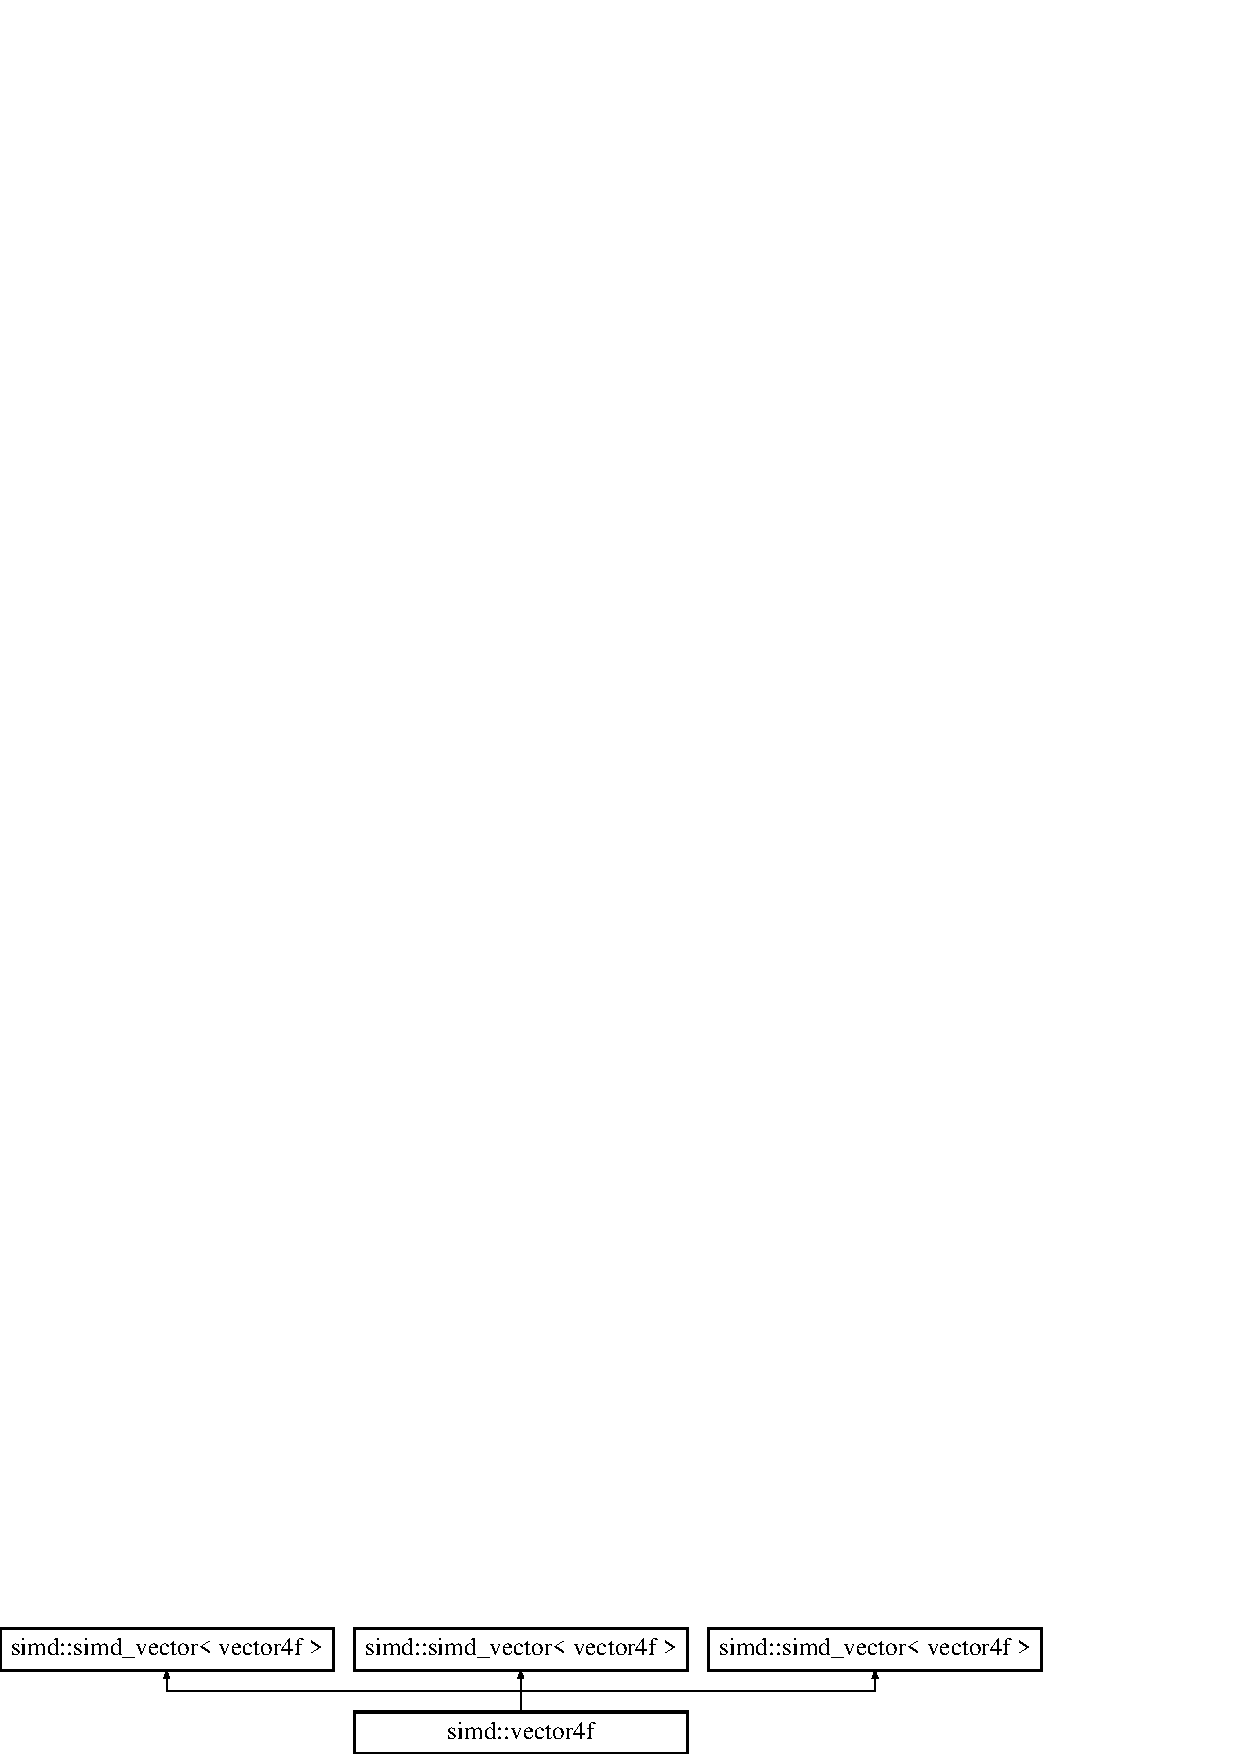
\includegraphics[height=1.964912cm]{classsimd_1_1vector4f}
\end{center}
\end{figure}
\subsection*{Public Member Functions}
\begin{DoxyCompactItemize}
\item 
\hypertarget{classsimd_1_1vector4f_a8cd2fc3260d14c0c67940a983a69a6e0}{{\bfseries vector4f} (float f)}\label{classsimd_1_1vector4f_a8cd2fc3260d14c0c67940a983a69a6e0}

\item 
\hypertarget{classsimd_1_1vector4f_a851a8e9f17c7608f082a110d48511d9d}{{\bfseries vector4f} (float f0, float f1, float f2, float f3)}\label{classsimd_1_1vector4f_a851a8e9f17c7608f082a110d48511d9d}

\item 
\hypertarget{classsimd_1_1vector4f_acfe638dab1c1d516989304bd62b87522}{{\bfseries vector4f} (const \+\_\+\+\_\+m128 \&rhs)}\label{classsimd_1_1vector4f_acfe638dab1c1d516989304bd62b87522}

\item 
\hypertarget{classsimd_1_1vector4f_ac6b2d78f7edf02288544a273109f7bce}{\hyperlink{classsimd_1_1vector4f}{vector4f} \& {\bfseries operator=} (const \+\_\+\+\_\+m128 \&rhs)}\label{classsimd_1_1vector4f_ac6b2d78f7edf02288544a273109f7bce}

\item 
\hypertarget{classsimd_1_1vector4f_a433d39bba6d70a4406fb70315d1d700c}{{\bfseries operator \+\_\+\+\_\+m128} () const }\label{classsimd_1_1vector4f_a433d39bba6d70a4406fb70315d1d700c}

\item 
\hypertarget{classsimd_1_1vector4f_a3f144eedb574683f0a74c816f06da9b5}{\hyperlink{classsimd_1_1vector4f}{vector4f} \& {\bfseries load\+\_\+a} (const float $\ast$src)}\label{classsimd_1_1vector4f_a3f144eedb574683f0a74c816f06da9b5}

\item 
\hypertarget{classsimd_1_1vector4f_a96eb6874cdcc0da473900f7798219ef0}{\hyperlink{classsimd_1_1vector4f}{vector4f} \& {\bfseries load\+\_\+u} (const float $\ast$src)}\label{classsimd_1_1vector4f_a96eb6874cdcc0da473900f7798219ef0}

\item 
\hypertarget{classsimd_1_1vector4f_a9084f345c629897c16c73858b112677d}{void {\bfseries store\+\_\+a} (float $\ast$dst) const }\label{classsimd_1_1vector4f_a9084f345c629897c16c73858b112677d}

\item 
\hypertarget{classsimd_1_1vector4f_ab7bc248d1ac6e5dbc7aba78034063ac1}{void {\bfseries store\+\_\+u} (float $\ast$dst) const }\label{classsimd_1_1vector4f_ab7bc248d1ac6e5dbc7aba78034063ac1}

\item 
\hypertarget{classsimd_1_1vector4f_a8cd2fc3260d14c0c67940a983a69a6e0}{{\bfseries vector4f} (float f)}\label{classsimd_1_1vector4f_a8cd2fc3260d14c0c67940a983a69a6e0}

\item 
\hypertarget{classsimd_1_1vector4f_a851a8e9f17c7608f082a110d48511d9d}{{\bfseries vector4f} (float f0, float f1, float f2, float f3)}\label{classsimd_1_1vector4f_a851a8e9f17c7608f082a110d48511d9d}

\item 
\hypertarget{classsimd_1_1vector4f_acfe638dab1c1d516989304bd62b87522}{{\bfseries vector4f} (const \+\_\+\+\_\+m128 \&rhs)}\label{classsimd_1_1vector4f_acfe638dab1c1d516989304bd62b87522}

\item 
\hypertarget{classsimd_1_1vector4f_ac6b2d78f7edf02288544a273109f7bce}{\hyperlink{classsimd_1_1vector4f}{vector4f} \& {\bfseries operator=} (const \+\_\+\+\_\+m128 \&rhs)}\label{classsimd_1_1vector4f_ac6b2d78f7edf02288544a273109f7bce}

\item 
\hypertarget{classsimd_1_1vector4f_a433d39bba6d70a4406fb70315d1d700c}{{\bfseries operator \+\_\+\+\_\+m128} () const }\label{classsimd_1_1vector4f_a433d39bba6d70a4406fb70315d1d700c}

\item 
\hypertarget{classsimd_1_1vector4f_a3f144eedb574683f0a74c816f06da9b5}{\hyperlink{classsimd_1_1vector4f}{vector4f} \& {\bfseries load\+\_\+a} (const float $\ast$src)}\label{classsimd_1_1vector4f_a3f144eedb574683f0a74c816f06da9b5}

\item 
\hypertarget{classsimd_1_1vector4f_a96eb6874cdcc0da473900f7798219ef0}{\hyperlink{classsimd_1_1vector4f}{vector4f} \& {\bfseries load\+\_\+u} (const float $\ast$src)}\label{classsimd_1_1vector4f_a96eb6874cdcc0da473900f7798219ef0}

\item 
\hypertarget{classsimd_1_1vector4f_a9084f345c629897c16c73858b112677d}{void {\bfseries store\+\_\+a} (float $\ast$dst) const }\label{classsimd_1_1vector4f_a9084f345c629897c16c73858b112677d}

\item 
\hypertarget{classsimd_1_1vector4f_ab7bc248d1ac6e5dbc7aba78034063ac1}{void {\bfseries store\+\_\+u} (float $\ast$dst) const }\label{classsimd_1_1vector4f_ab7bc248d1ac6e5dbc7aba78034063ac1}

\item 
\hypertarget{classsimd_1_1vector4f_a8cd2fc3260d14c0c67940a983a69a6e0}{{\bfseries vector4f} (float f)}\label{classsimd_1_1vector4f_a8cd2fc3260d14c0c67940a983a69a6e0}

\item 
\hypertarget{classsimd_1_1vector4f_a851a8e9f17c7608f082a110d48511d9d}{{\bfseries vector4f} (float f0, float f1, float f2, float f3)}\label{classsimd_1_1vector4f_a851a8e9f17c7608f082a110d48511d9d}

\item 
\hypertarget{classsimd_1_1vector4f_acfe638dab1c1d516989304bd62b87522}{{\bfseries vector4f} (const \+\_\+\+\_\+m128 \&rhs)}\label{classsimd_1_1vector4f_acfe638dab1c1d516989304bd62b87522}

\item 
\hypertarget{classsimd_1_1vector4f_ac6b2d78f7edf02288544a273109f7bce}{\hyperlink{classsimd_1_1vector4f}{vector4f} \& {\bfseries operator=} (const \+\_\+\+\_\+m128 \&rhs)}\label{classsimd_1_1vector4f_ac6b2d78f7edf02288544a273109f7bce}

\item 
\hypertarget{classsimd_1_1vector4f_a433d39bba6d70a4406fb70315d1d700c}{{\bfseries operator \+\_\+\+\_\+m128} () const }\label{classsimd_1_1vector4f_a433d39bba6d70a4406fb70315d1d700c}

\item 
\hypertarget{classsimd_1_1vector4f_a3f144eedb574683f0a74c816f06da9b5}{\hyperlink{classsimd_1_1vector4f}{vector4f} \& {\bfseries load\+\_\+a} (const float $\ast$src)}\label{classsimd_1_1vector4f_a3f144eedb574683f0a74c816f06da9b5}

\item 
\hypertarget{classsimd_1_1vector4f_a96eb6874cdcc0da473900f7798219ef0}{\hyperlink{classsimd_1_1vector4f}{vector4f} \& {\bfseries load\+\_\+u} (const float $\ast$src)}\label{classsimd_1_1vector4f_a96eb6874cdcc0da473900f7798219ef0}

\item 
\hypertarget{classsimd_1_1vector4f_a146d26ac180a2165ffbc35ff1301747f}{\hyperlink{classsimd_1_1vector4f}{vector4f} \& {\bfseries load1} (const float $\ast$src)}\label{classsimd_1_1vector4f_a146d26ac180a2165ffbc35ff1301747f}

\item 
\hypertarget{classsimd_1_1vector4f_a9084f345c629897c16c73858b112677d}{void {\bfseries store\+\_\+a} (float $\ast$dst) const }\label{classsimd_1_1vector4f_a9084f345c629897c16c73858b112677d}

\item 
\hypertarget{classsimd_1_1vector4f_ab7bc248d1ac6e5dbc7aba78034063ac1}{void {\bfseries store\+\_\+u} (float $\ast$dst) const }\label{classsimd_1_1vector4f_ab7bc248d1ac6e5dbc7aba78034063ac1}

\end{DoxyCompactItemize}
\subsection*{Additional Inherited Members}


The documentation for this class was generated from the following file\+:\begin{DoxyCompactItemize}
\item 
A\+T\+L2/S\+I\+M\+D.\+hpp\end{DoxyCompactItemize}

\hypertarget{classatl_1_1_variable_info_1_1_v_i_spin_lock}{\section{atl\+:\+:Variable\+Info$<$ R\+E\+A\+L\+\_\+\+T $>$\+:\+:V\+I\+Spin\+Lock Class Reference}
\label{classatl_1_1_variable_info_1_1_v_i_spin_lock}\index{atl\+::\+Variable\+Info$<$ R\+E\+A\+L\+\_\+\+T $>$\+::\+V\+I\+Spin\+Lock@{atl\+::\+Variable\+Info$<$ R\+E\+A\+L\+\_\+\+T $>$\+::\+V\+I\+Spin\+Lock}}
}
\subsection*{Public Member Functions}
\begin{DoxyCompactItemize}
\item 
\hypertarget{classatl_1_1_variable_info_1_1_v_i_spin_lock_a957f7fa52c1c3647c74697b8718abfc0}{void {\bfseries lock} ()}\label{classatl_1_1_variable_info_1_1_v_i_spin_lock_a957f7fa52c1c3647c74697b8718abfc0}

\item 
\hypertarget{classatl_1_1_variable_info_1_1_v_i_spin_lock_aa7bb227ca73abf2218b16938a6fc29fa}{void {\bfseries unlock} ()}\label{classatl_1_1_variable_info_1_1_v_i_spin_lock_aa7bb227ca73abf2218b16938a6fc29fa}

\end{DoxyCompactItemize}


The documentation for this class was generated from the following file\+:\begin{DoxyCompactItemize}
\item 
Variable\+Info.\+hpp\end{DoxyCompactItemize}

\hypertarget{classatl_1_1_wait_variable}{\section{atl\+:\+:Wait\+Variable Class Reference}
\label{classatl_1_1_wait_variable}\index{atl\+::\+Wait\+Variable@{atl\+::\+Wait\+Variable}}
}


{\ttfamily \#include $<$Thread\+Pool.\+hpp$>$}

\subsection*{Friends}
\begin{DoxyCompactItemize}
\item 
\hypertarget{classatl_1_1_wait_variable_ac4810fd904928605bdb3f8606ffe5ec4}{class {\bfseries Thread\+Pool}}\label{classatl_1_1_wait_variable_ac4810fd904928605bdb3f8606ffe5ec4}

\end{DoxyCompactItemize}


\subsection{Detailed Description}
\hyperlink{classatl_1_1_wait_variable}{Wait\+Variable} is used in conjunction with \hyperlink{classatl_1_1_thread_pool}{Thread\+Pool} runs where it is desired to wait for threads to complete before continuing. 

The documentation for this class was generated from the following file\+:\begin{DoxyCompactItemize}
\item 
A\+T\+L2/Thread\+Pool.\+hpp\end{DoxyCompactItemize}

%--- End generated contents ---

% Index
\newpage
\phantomsection
\addcontentsline{toc}{chapter}{Index}
\printindex

\end{document}
